%% -*- coding:utf-8 -*-
%%%%%%%%%%%%%%%%%%%%%%%%%%%%%%%%%%%%%%%%%%%%%%%%%%%%%%%%%
%%   $RCSfile: hpsg-lehrbuch-include.tex,v $
%%  $Revision: 1.16 $
%%      $Date: 2008/09/30 09:14:41 $
%%     Author: Stefan Mueller (CL Uni-Bremen)
%%    Purpose: 
%%   Language: LaTeX
%%%%%%%%%%%%%%%%%%%%%%%%%%%%%%%%%%%%%%%%%%%%%%%%%%%%%%%%%

%\hypersetup{bookmarksopenlevel=0}






%\renewcommand{\centerfit}[1]{}


\provideboolean{hpsg-buch}
\setboolean{hpsg-buch}{true}

\PassOptionsToPackage{main=ngerman}{babel}

\begin{document} 

%\lsBookLanguageGerman

% \mmzset{
%   deactivate=\todo,
% }


\mmzset{disable}
\maketitle
\frontmatter
\mmzset{enable}

\currentpdfbookmark{Inhaltsverzeichnis}{toc} % adds a PDF bookmark
\tableofcontents



%% -*- coding:utf-8 -*-

\chapter*{Vorwort}

\begin{sloppypar}
Seit 1994 unterrichte ich die Kopfgesteuerte Phrasenstrukturgrammatik (Head-Driven Phrase
Structure Grammar). In den ersten Jahren habe ich dazu ein Vorlesungsskript verwendet, das
dann in \citew{Mueller99a} eingeflossen ist. Dieses Buch ist allerdings komplex und
für eine Einführung wohl weniger geeignet. Ich habe mich also entschlossen, ein Lehrbuch zu
schreiben, das sich auf das Wesentliche konzentriert und Problemfälle nicht erörtert.
\end{sloppypar}

Das Buch sollte für alle verständlich sein, die mit Wortarten und dem Valenzbegriff vertraut
sind. Nach der Lektüre dieses Buches soll der Leser bzw.\ die Leserin in der Lage sein, aktuelle
HPSG"=Publikationen zu verstehen. Ziel ist es deshalb, die aktuelle Merkmalsgeometrie zu motivieren
und darzustellen, wie zentrale Konzepte wie Valenz und Selektion, Modifikation und lexikalische
Prozesse modelliert werden.

In jedem der Kapitel wird ein bestimmter Aspekt der Theorie behandelt, weshalb die Kapitel teilweise
recht kurz sind. Die Kapitel bestehen aus der Besprechung des jeweiligen Aspekts, eventuell einer
Diskussion alternativer Theorien, einem kurzen Abschnitt mit Kontrollfragen, einem Abschnitt
mit Übungsaufgaben und bei einigen Kapiteln Hinweisen zu weiterführender Literatur. Die Diskussion
alternativer Theorien ist für den fortgeschrittenen Leser gedacht, 
dem eine Bewertung der HPSG im gegenwärtigen Forschungsumfeld wichtig ist. Die Argumentation
bezieht sich mitunter auf Konzepte, die in diesem Buch nicht ausführlich dargestellt werden können.
Es gibt dann immer Verweise auf weiterführende Literatur. Für einen ersten Überblick über
die HPSG kann man die Diskussionsabschnitte überspringen und eventuell später beim vertiefenden
Lesen zu einzelnen Abschnitten zurückkehren.

\begin{sloppy}
Zu diesem Buch gehört ein Foliensatz, der unter 
\url{https://hpsg.hu-berlin.de/~stefan/Lehre/HPSG/}
verfügbar ist. Von dieser Seite gelangt man auch zu einer Seite, die computerverarbeitbare
Grammatiken enthält, die den jeweiligen Ka\-pi\-teln in diesem Buch entsprechen. Eine CD, die
alle zum Grammatikentwickeln benötigte Software und auch die Grammatiken enthält, ist unter
\url{https://hpsg.hu-berlin.de/Software/Grammix/} verfügbar. Dem interessierten Leser
wird nahegelegt, sich mit den Grammatiken zu beschäftigen, da das anschaulicher ist,
als es jeder noch so gute Text sein könnte.
\end{sloppy}

\section*{Benutzte Korpora}

Die meisten der Beispiele in diesem Buch sind Belege aus der {\em taz}\footnote{
\url{http://www.taz.de/}, 21.07.2024.}, einer überregionalen
deutschen Tageszeitung. Andere sind aus dem Magazin \emph{Der Spiegel},
aus der Computerzeitschrift c't oder aus der \emph{zitty}, einer kleinen Zeitschrift mit
Veranstaltungshinweisen aus Berlin. 
%% Auch Beispiele aus Romanen oder wissenschaftlichen Texten über
%% Linguistik wurden berücksichtigt. I have also considered examples from novels
%% and some from scientific texts on linguistics. Of course, it is clear to
%% me that the language of linguists changes according to their research topic
%% and according to the theories they have at a certain stage, but in many cases
%% I have quoted examples that show that a claim of the author is wrong and this excludes
%% the possibility that the production of the respective sentences was influenced
%% by the author's theoretical work.


Es ist sehr bequem, elektronische Korpora zu verwenden, um bestimmte Behauptungen zu rechtfertigen
oder zu widerlegen.
Für diese Zwecke habe ich die taz-CD"=Roms benutzt, die über 20 Jahrgänge der Zeitung enthalten.
Außerdem habe ich das \cosmas"=Korpus\footnote{\url{https://cosmas2.ids-mannheim.de/cosmas2-web/}, 21.07.2024.} 
verwendet, das vom Institut für Deutsche Sprache (IDS) Mannheim zur Verfügung gestellt
wird. Die Version, die über das World Wide Web zugänglich ist, enthält 1,489 Milliarden Wörter.
Neben \cosmas habe ich das \negra{}\hyp Korpus der Universität Saarbrücken,
% \footnote{
% \url{http://www.coli.uni-sb.de/sfb378/negra-corpus/}}
das Tiger"=Korpus des Instituts für maschinelle Sprachverarbeitung der Universität Stuttgart,
%\footnote{\url{http://www.ims.uni-stuttgart.de/projekte/TIGER/TIGERCorpus/}}
und das Digitale Wörterbuch der deutschen Sprache\footnote{\url{http://www.dwds.de/}, 21.07.2024.} der 
Berlin"=Brandenburgischen Akademie der Wissenschaften benutzt.

~\medskip

\noindent
Bremen, 12.\ Februar, 2007\hfill Stefan Müller

\section*{Vorwort zur zweiten Auf"|lage}

Die zweite Auf"|lage unterscheidet sich nur geringfügig von der ersten. Ich habe einige
Literaturverweise ergänzt und einige erklärende Sätze eingefügt. Die Diskussion der
vererbungsbasierten Analyse des Passivs in Abschnitt~\ref{sec-vererbung-koenig} habe ich geändert und
die Beispiele aus dem Yukatekischen\il{Yukatekisch} durch Beispiele aus dem Türkischen\il{Türkisch}
ersetzt. Zur Motivation siehe \citew[\page 387]{Mueller2007d}. Die Analyse von Zeitausdrücken im
Akkusativ wurde entfernt, da man sie nicht -- wie in der ersten Auf"|lage vorgeschlagen -- an Lexikoneinträgen festmachen kann 
(siehe Seite~\pageref{bsp-den-groessten-Teil-der-Woche}).


~\medskip

\noindent
Berlin, 01.\ August, 2008\hfill Stefan Müller

\section*{Vorwort zur dritten Auf"|lage}

Die wichtigste Änderung von der zweiten zur dritten Auf"|lage besteht in einer Anpassung des
Kopf"=Argument"=Schemas. Ich verwende jetzt nicht mehr die \emph{del}"=Relation sondern
\emph{append} \citep[Abschnitt~8.4]{MuellerGTBuch1}. Das ermöglicht eine einfache sprachübergreifende Analyse der Konstituentenstellung
\citep{MuellerCopula}. Die entsprechenden Analysen haben sich im CoreGram"=Projekt\footnote{
  \url{https://hpsg.hu-berlin.de/Projects/CoreGram.html}. Zu einer Beschreibung des Projekts siehe \citew{MuellerCoreGram}. Das CoreGram"=Projekt beschäftigt sich mit der Implementation von Grammatiken für so
verschiedene Sprachen wie Deutsch, Dänisch\il{Dänisch}
\citep{MOe2011a,MuellerPredication,MuellerCopula,MOeDanish}, Englisch\il{Englisch}
\citep{MuellerPredication,MuellerCopula}, Jiddisch\il{Jiddisch} \citep{MOe2011a}, Spanisch\il{Spanisch}, Französisch\il{Französisch},
Maltesisch\il{Maltesisch} \citep{MuellerMalteseSketch},
Persisch\il{Persisch} \citep{MuellerPersian} und Mandarin Chinesisch\il{Mandarin Chinesisch} \citep{Lipenkova2009a,ML2009a}.
}, bewährt. 

Wir haben uns entschlossen, die CD-Rom, die bisher mit dem Buch zusammen ausgeliefert wurde, nicht
mehr gemeinsam mit dem Buch zu vertreiben. Die Grammaix-CD \citep{Mueller2007b} ist im Netz verfügbar\footnote{
  \url{https://hpsg.hu-berlin.de/Software/Grammix/}
} und die Netzverbindungen sind inzwischen so gut, dass man sich CDs herunterladen kann. Denjenigen,
die über keine ausreichend schnelle Internetanbindung verfügen, schicken wir gern eine CD zu (bitte
mein Sekretariat kontaktieren). 
Die Änderung des Kopf"=Argument"=Schemas ist auf der Grammix"=CD in der gegenwärtig auf der
Web-Seite verfügbaren Version noch nicht enthalten. Die Grammix"=CD
wird komplett umgestaltet: Es wird ein neues Betriebssystem geben, eine neue wesentlich verbesserte
und effizientere Version von TRALE und die Grammatiken aus dem CoreGram"=Projekt. Ich hoffe, die
Arbeiten an der neue Version der CD noch vor der Fertigstellung des Berliner Flughafens abschließen
zu können.\footnote{Fußnote aus der Zukunft: Bis zur Eröffnung des BER am 31.10.2020 war noch
  ausreichend Zeit. 2013, also sieben Jahre vor der Eröffnung des BER, habe ich eine Virtuelle
  Maschine mit Grammix zum Download bereitgestellt.} Die angepassten Lehrbuchgrammatiken und die Grammatiken aus dem CoreGram"=Projekt sind
aber bereits jetzt über meine Webseite zugänglich.

Der Abschnitt~\ref{sec-vererbung-koenig} zur vererbungsbasierten Analyse des Passivs wurde nochmals
überarbeitet und enthält jetzt auch eine Diskussion von Doppeltpassivierungen im Türkischen\il{Türkisch} und
anderen Sprachen. Außerdem habe ich im Abschnitt~\ref{sec-spr} etwas erklärenden Text und eine
Abbildung hinzugefügt. Die Diskussion des \textsc{mother}"=Merkmals im Kapitel~\ref{Kapitel-Lokalität} wurde erweitert und auf
den Stand von \citew{MuellerGTBuch1} bzw.\ \citew{MuellerGTBuch2} gebracht. 
Ein Fehler in den Schemata~\ref{schema-bin-mark} und~\ref{schema-bin-mark-final} wurde korrigiert.

Es gibt jetzt einen Anhang mit Lösungen zu ausgewählten Übungsaufgaben.


~\medskip

\noindent
Berlin, 23. Januar 2013\hfill Stefan Müller


\section*{Vorwort zur vierten Auf"|lage}

Dieses Buch hat eine lange Geschichte. Es ist in den Jahren 2005–2006 aus Folien entstanden, die ich
ab 1994 für die Lehre benutzt habe. Meine Dissertation habe ich 1999 bei Niemeyer
veröffentlicht. Das Buch war bis zur Veröffentlichung auf meiner Webseite verfügbar. Danach musste
ich es von der Webseite entfernen. Die Veröffentlichung war also eine Entöffentlichung. Der Preis
war mit 186 DM für 486 Seiten prohibitiv hoch: Privatpersonen dürften sich das Buch höchst selten
gekauft haben. Inzwischen wurde Niemeyer von De Gruyter geschluckt und De Gruyter bietet das Buch für 150€
an. Das Buch habe ich selbst geschrieben und komplett selbst gesetzt. Mit meinem neuen Buch sollte das nicht passieren,
weshalb ich vorhatte, es bei einem unbekannten Print-On-Demand-Verlag zu veröffentlichen. Auf einer
Konferenz sprach ich mit Brigitte Narr über meine Pläne und sie sagte: "`Machen Sie das
nicht!"'. Wir kamen überein, dass ich das Buch im Stauffenburg-Verlag veröffentliche und es
gleichzeitig auf meiner Web-Seite lassen kann. Ich habe Frau Narrs Kontonummer auf meiner Web-Seite
angegeben und weiß von einigen berühmten Grammatikern, dass sie Frau Narr auch Geld überwiesen
haben. (Andere Grammatiker*innen waren so freundlich Frau Narr darauf hinzuweisen, dass ich das Buch
kostenlos zum Download auf meiner Web-Seite anbiete \ldots). 

Ich habe dann auch mein Grammatiktheorie"=Buch im Stauffenburg"=Verlag veröffentlicht. Ab 2012 habe
ich gemeinsam mit Martin Haspelmath und mit der Unterstützung von vielen, vielen Linguist*innen
weltweit (u.\,a.\ Chomsky, Pinker, Goldberg) begonnen, einen wissenschaftsgeführten Diamond Open
Access-Verlag aufzubauen \citep{MuellerOA}.\footnote{Diamond Open Access bedeutet, dass weder die Autor*innen noch die
Leser*innen für die Veröffentlichungen bezahlen müssen.} Seit 2014 gibt es Language Science Press. Ab diesem Zeitpunkt habe ich
auch meine Bücher dort veröffentlicht. 

Im April 2024 habe ich Frau Narr
gefragt, ob ich die Rechte an diesem Buch zurückbekommen könnte, und sie hat eingewilligt. Das Buch
ist jetzt also wie fast alle meine Bücher frei und ich kann es unter der CC-BY-Lizenz bei Language
Science Press veröffentlichen.

Seit 2013 hat sich einiges getan. Ich habe mich weiter mit sprachübergreifenden Fragestellungen
beschäftigt und ein Buch über germanische Sprachen veröffentlicht \citep{MuellerGermanic}. Dort habe
ich alle germanischen Sprachen so analysiert, dass die Verben in den jeweiligen Sprachen dieselbe
Argumentstruktur haben. Zum Beispiel sind die Gegenstücke zum deutschen \emph{geben} ebenfalls
dreistellig. Die Argumentstrukturen unterscheiden sich lediglich in den Kasus: Das Englische hat keinen
Dativ; die Sprachen haben unterschiedliche Verteilungen von strukturellem und lexikalischem
Kasus. Ich nehme, wie in neueren Arbeiten üblich, eine Argumentstruktur"=Liste (\argst) an, auf der 
alle Argumente eines Kopfes aufgelistet sind. Die Argumente werden von dieser Repräsentation auf
Valenzmerkmale gemappt. Diese sind \spr für Spezifikatoren und \comps für Komplemente. Die
Reihenfolge der drei Argumente in der \argst ist für alle germanischen Sprachen gleich. Sie
entspricht der Normalstellung im Deutschen (Nominativ, Dativ, Akkusativ) und der Stellung im
Englischen:
\eal
\ex dass er dem Affen den Stock gibt
\ex that he gives the monkey the stick
\zl
Das ist ein Unterschied zu früheren Auf"|lagen des Buches, in denen die Elemente in der Valenzliste
\subcat in der Reihenfolge Nominativ, Akkusativ, Dativ angeordnet waren. Die Einführung in
Phrasenstrukturgrammatiken und die Analyse der Linearisierungstheorien in Abschnitt~\ref{sec-konstituentenreihenfolge-alternativen} wurden an
diese veränderte Grundreihenfolge angepasst.

Das Semantik"=Kapitel wurde komplett überarbeitet. Statt der Situationssematik, die in den ersten
drei Auf\/lagen des Buches verwendet wurde, gibt es im Kapitel~\ref{Kapitel-Semantik} nun eine
Einführung in die Minimal Recursion Semantics \citep*{CFPS2005a}.

Ansonsten habe ich das Buch jetzt auf neue Rechtschreibung umgestellt, ich habe begonnen zu gendern
und habe die meisten Beispiele so abgeändert, dass es keine Gender-Stereotypen mehr gibt
\citep{MB97a,PCKSDMC2017a}. Für das Deutsche ist das leider nicht so einfach, weil man auf die
Verwendung von Maskulina angewiesen ist, denn nur bei diesen ist der Kasus voll ausbuchstabiert. 

Ich habe an Stellen, wo das noch nicht der Fall war, bei Literaturquellen Seitenzahlen hinzugefügt.

% ein Komma und Optionalität bei Valenz von denken
% Bei Anja Herrmann bedanke ich mich für den Hinweis auf Typos und Fragen zu den Übungsaufgaben.

% 23.05.2022 Im Kausus-Kapitel Verweis auf 2 statt auf 1. Karla Jerabeck hats gefunden.
% 19) a. Er goß ihr die Blumen.
%     b. Er zündete ihr das Haus an.
% Wegener (1985a) hat jedoch gezeigt, dass diese Dative Komplementstatus haben.
%
% Erklären, wieso Komplementstatus.

% Lexikon Typhierarchie statt acc dat. 03.06.2024

% Den Kindern wurde geholfen -> Den Kindern wird geholfen.
% Beispiele wurden fehlerhaft Haider zugeschrieben. 07.06.2024

% 11.06.2024
% Bei Lösungen wurde der Numerus-Wert bei der Adjektivlexikonregel entfernt. Dieser
% wird von der Endung bestimmt, die beim attributiven Adjektiv angehängt wird. Kasus und Genus
% wurden in der Aufgabenstellung wieder eingebaut, aber mit Anmerkung versehen, dass sie weggelassen
% werden sollen.

%21.06.2024 

% Reihenfolge im Abschnitt über Linearisierungstheorien wurde an nom, dat, acc angepasst.

% To do:
%
% Sophie Reule, Studentin 22.01.2018
% Auf S. 74 des HPSG-Lehrbuchs werden die Elemente der Liste Phon durch Kommata getrennt, zuvor war
% dies nicht der Fall. Welche Bedeutung hat die Notation an dieser Stelle? 

% 
% Auf Seite 75 wird vom SYNSEM-Wert gesprochen, der wurde aber gar nicht eingeführt.

% Wert von PSOA-ARG ist eine Liste, also muss Mörder in eine Liste in (21) Kapitel 6.4

% 17.05.18 Auf S. 282 war ein "ist" doppelt.

% 28.08.2018 Steve Wechsler: Kongruenzmerkmale des Nomens müssen Kopfmerkmale sein,
% denn wenn es Depiktive gibt, die mit Nomina kongruieren, müssen deren CONCORD-Merkmale nach außen
% verfügbar sein.

%On p.237 of your HPSG Lehrbuch (3rd edition) you're saying:

%% Przepiórkowski (1999a) integriert deshalb Meurers Ansatz der Kasuszuweisung (1999b;
%% 2000, Kapitel 10.4.1.4) in seine Theorie und führt zusätzlich zum REALIZED -Merkmal das
%% Merkmal RAISED ein, das den Wert + hat, wenn ein Argument angehoben wird, und den
%% Wert −, wenn das nicht der Fall ist.

%% The following part is false:

%% führt zusätzlich zum REALIZED -Merkmal das Merkmal RAISED ein

%% Rather, RAISED replaces REALIZED.

%% Please, remember when you prepare the 4th edition ;-)


~\medskip

\noindent
Berlin, \today\hfill Stefan Müller
% \include{chapters/acknowledgments}
% \include{chapters/abbreviations} 

\mainmatter
%% -*- coding:utf-8 -*-
%%%%%%%%%%%%%%%%%%%%%%%%%%%%%%%%%%%%%%%%%%%%%%%%%%%%%%%%%
%%   $RCSfile: 1-hpsg-einleitung.tex,v $
%%  $Revision: 1.19 $
%%      $Date: 2008/09/30 09:14:41 $
%%     Author: Stefan Mueller (CL Uni-Bremen)
%%    Purpose: 
%%   Language: LaTeX
%%%%%%%%%%%%%%%%%%%%%%%%%%%%%%%%%%%%%%%%%%%%%%%%%%%%%%%%%


\chapter{Einleitung}

In diesem Kapitel soll erklärt werden, warum man sich überhaupt mit Syntax
beschäftigt (Abschnitt~\ref{sec-wozu-syntax}) und 
warum es sinnvoll ist, die Erkenntnisse zu formalisieren (Abschnitt~\ref{sec-formal}).
Einige Grundbegriffe werden in den Abschnitten~\ref{konstituententests}--\ref{sec-intro-arg-adj} eingeführt. 
Die Abschnitte~\ref{sec-grammatikmodelle}--\ref{sec-xbar}
beschäftigen sich mit Vorgängertheorien, die die HPSG beeinflusst haben.
Im Abschnitt~\ref{sec-grundlegendes} werden einige Eigenschaften der HPSG
vorgestellt, insbesondere die Modellierung sprachlicher Äußerungen mittels
Merkmalstrukturen. Dieser Abschnitt dient zur Überleitung ins nächste Kapitel,
in dem dann der Formalismus der Merkmalstrukturen vorgestellt wird.

\section{Wozu Syntax?}
\label{sec-wozu-syntax}

Die sprachlichen Ausdrücke, die wir verwenden, haben eine Bedeutung. Es handelt
sich um sogenannte Form"=Bedeutungspaare \citep{Saussure16a-de}. Dem Wort \emph{Baum}
mit seiner bestimmten orthographischen Form oder einer entsprechenden Aussprache
wird die Bedeutung \emph{baum}$'$ zugeordnet. Aus kleineren sprachlichen Einheiten
können größere gebildet werden: Wörter können zu Wortgruppen verbunden werden
und diese zu Sätzen.

Die Frage, die sich nun stellt, ist folgende: Braucht man ein formales System, das
diesen Sätzen eine Struktur zuordnet? Würde es nicht ausreichen, so wie wir
für \emph{Baum} ein Form"=Bedeutungspaar haben, entsprechende Form"=Bedeutungspaare
für Sätze aufzuschreiben?\label{Seite-Alle-Sätze-aufschreiben} Das wäre im Prinzip möglich, wenn eine Sprache eine
endliche Aufzählung von Wortfolgen wäre. Nimmt man an,
dass es eine maximale Satzlänge und eine maximale Wortlänge und somit eine endliche
Anzahl von Wörtern gibt, so ist die Anzahl der bildbaren Sätze endlich.
Allerdings ist die Zahl der bildbaren Sätze selbst bei Begrenzung der Satzlänge riesig.
Und die Frage, die man dann beantworten muss, ist: Was ist die Maximallänge für
Sätze? Zum Beispiel kann man die Sätze in (\mex{1}) verlängern:
\eal
\ex Dieser Satz geht weiter und weiter und weiter und weiter \ldots
\ex {}[Ein Satz ist ein Satz] ist ein Satz.
\zl
In (\mex{0}b) wird etwas über die Wortgruppe \emph{ein Satz ist ein Satz} ausgesagt, nämlich dass sie
ein Satz ist. Genau dasselbe kann man natürlich auch vom gesamten Satz (\mex{0}b) behaupten und den Satz
entsprechend um \emph{ist ein Satz} erweitern.

Durch Erweiterungen wie die in (\mex{0}) können wir enorm lange und komplexe Sätze bilden.\footnote{
Manchmal wird behauptet, dass wir in der Lage wären, unendlich lange Sätze zu bilden (\citealp*[\page
 117]{NKN2001a}, \citealp[\page 3]{KS2008a-u}, Dan Everett in \citew{OW2012a} bei 25:19,
 \citealp*[\page 67]{Chesi2015a-u}, \citealp[\page 5]{Lin2017a}, \citealp[\page 2]{Martorell2018a}.
 \href{https://en.wikipedia.org/wiki/Biolinguistics\#Minimalist_Program}{Wikipedia-Eintrag für
   Biolinguistics/Minimalism}, 2019-10-17)
% was there till 2019-11-03 fixed on 2019-11-09 
% https://en.wikipedia.org/w/index.php?title=Biolinguistics&oldid=924370751
% "This mechanism allows people to combine words into infinite strings."
 oder dass Chomsky so etwas behauptet hätte \citep[\page 341]{Leiss2003a}.

Das ist nicht richtig, da jeder Satz irgendwann einmal enden
 muss. Auch in der Theorie der formalen Sprachen in der Chomskyschen Tradition gibt es keinen
 unendlich langen Satz, vielmehr wird von bestimmten formalen Grammatiken eine Menge mit unendlich
 vielen endlichen Sätzen beschrieben (\citealp[\page 13]{Chomsky57a}). Zu Rekursion\is{Rekursion} in
 der Grammatik und Behauptungen zur Unendlichkeit unserer Sprache siehe auch \citew{PS2010a} und
 \citew[Abschnitt~11.1.1.8]{MuellerGTBuch1}.
} Die Festsetzung einer Grenze, bis zu der solche Kombinationen zu unserer Sprache gehören, wäre
willkürlich \parencites[\page 208]{Harris57a}[\page 23]{Chomsky57a}. Auch ist die Annahme, dass
solche komplexen Sätze als Gesamtheit in unserem Gehirn gespeichert sind, unplausibel. Man kann für
hochfrequente Muster bzw.\ idiomatische Kombinationen mit psycholinguistischen Experimenten zeigen,
dass sie als ganze Einheit gespeichert sind, das ist für Sätze wie die in (\mex{0}) jedoch nicht der
Fall. Es muss also eine Strukturierung der Äußerungen, es muss bestimmte wiederkehrende Muster
geben. Solche Muster aufzudecken, zu beschreiben und zu erklären, ist die Aufgabe der Syntax.

Wenn man nicht annehmen will, dass Sprache nur eine Liste von Form"=Bedeutungspaaren
ist, dann muss es ein Verfahren geben, die Bedeutung komplexer Äußerungen aus
den Bedeutungen der Bestandteile der Äußerungen zu ermitteln.
Die Syntax sagt etwas über die Art und Weise der Kombination der beteiligten
Wörter aus, etwas über die Struktur einer Äußerung.
So hilft uns zum Beispiel das Wissen über Subjekt"=Verb"=Kongruenz bei der Interpretation
der Sätze in (\mex{1}c,d):
\eal
\ex Die Frau schläft.
\ex Die Mädchen schlafen.
\ex Die Frau kennt  die Mädchen.
\ex Die Frau kennen die Mädchen.
\zl
Die Sätze in (\mex{0}a,b) zeigen, dass ein Subjekt im Singular bzw.\ Plural
ein entsprechend flektiertes Verb braucht. In (\mex{0}a,b) verlangt das Verb nur ein
Argument, so dass die Funktion von \emph{die Frau} bzw.\ \emph{die Mädchen} klar ist.
In (\mex{0}c,d) verlangt das Verb zwei Argumente, und \emph{die Frau} und \emph{die Mädchen}
könnten an beiden Argumentstellen auf"|treten. Die Sätze könnten also bedeuten, dass
die Frau jemanden kennt oder dass jemand die Frau kennt. Durch die Flexion des Verbs und
Kenntnis der syntaktischen Gesetzmäßigkeiten des Deutschen weiß der Hörer
aber, dass es für (\mex{0}c,d) jeweils nur eine Lesart gibt.



\section{Warum formal?}
\label{sec-formal}

Die folgenden beiden Zitate geben eine Begründung für die Notwendigkeit
formaler Beschreibung von Sprache:  
\begin{quote}
Precisely constructed models for linguistic structure can play an
important role, both negative and positive, in the process of discovery 
itself. By pushing a precise but inadequate formulation to
an unacceptable conclusion, we can often expose the exact source
of this inadequacy and, consequently, gain a deeper understanding
of the linguistic data. More positively, a formalized theory may 
automatically provide solutions for many problems other than those
for which it was explicitly designed. Obscure and intuition-bound
notions can neither lead to absurd conclusions nor provide new and
correct ones, and hence they fail to be useful in two important respects. 
I think that some of those linguists who have questioned
the value of precise and technical development of linguistic theory
have failed to recognize the productive potential in the method
of rigorously stating a proposed theory and applying it strictly to
linguistic material with no attempt to avoid unacceptable conclusions 
by ad hoc adjustments or loose formulation.
\citep[\page5]{Chomsky57a}
\end{quote}

\begin{quote}
As is frequently pointed out but cannot be overemphasized, an important goal
of formalization in linguistics is to enable subsequent researchers to see the defects
of an analysis as clearly as its merits; only then can progress be made efficiently.
\citep[\page322]{Dowty79a}
\end{quote}
%
Wenn wir linguistische Beschreibungen formalisieren, können wir leichter
erkennen, was genau eine Analyse bedeutet. Wir können feststellen, welche
Vorhersagen sie macht, und wir können alternative Analysen ausschließen.




\section{Konstituenten}
\label{konstituententests}

Betrachtet man den Satz in (\mex{1}), so hat man das Gefühl, dass bestimmte Wörter zu einer
Einheit gehören.
\ea
Alle Studenten lesen während der vorlesungsfreien Zeit Bücher.
\z
In diesem Abschnitt sollen Tests vorgestellt werden, die Indizien für eine engere
Zusammengehörigkeit von Wörtern darstellen. Wenn von einer \emph{Wortfolge}\is{Wortfolge}
die Rede ist, ist eine beliebige linear zusammenhängende Folge von Wörtern gemeint, 
die nicht unbedingt syntaktisch oder semantisch zusammengehörig sein müssen, \zb
\emph{Studenten lesen während} in (\mex{0}). Mehrere Wörter, die eine strukturelle Einheit bilden,
werden dagegen als \emph{Wortgruppe}\is{Wortgruppe}, \emph{Konstituente}\is{Konstituente}
oder \emph{Phrase}\is{Phrase} bezeichnet. Den Trivialfall stellen immer einzelne Wörter dar, die
natürlich immer eine strukturelle Einheit aus einem einzelnen Element bilden.

\subsection{Konstituententests}

Für den Konstituentenstatus gibt es Tests, die in den folgenden Abschnitten besprochen werden.
Wie im Abschnitt~\ref{sec-status-der-ktests} gezeigt werden wird, gibt es Fälle, bei denen die
blinde Anwendung der Tests zu unerwünschten Resultaten führt.

\subsubsection{Substituierbarkeit}

Kann man eine Wortfolge %einer bestimmten Kategorie 
in einem Satz gegen eine andere Wortfolge so austauschen,\is{Austauschbarkeit}\is{Substituierbarkeit} dass
wieder ein akzeptabler Satz entsteht, so ist das ein Indiz dafür, dass 
die beiden Wortfolgen Konstituenten bilden.

In (\mex{1}) kann man \emph{den Mann} durch \emph{eine Frau} ersetzen, was ein Indiz dafür
ist, dass beide Wortfolgen Konstituenten sind.
\eal
\ex Aicke kennt [den Mann].
\ex Aicke kennt [eine Frau].
\zl

\noindent
Genauso kann man in (\mex{1}a) die Wortfolge \emph{das Buch zu lesen} durch
\emph{dem Affen den Stock zu geben} ersetzen.
\eal
\ex Aicke versucht, das Buch zu lesen.\label{ex-das-buch-zu-lesen}
\ex Aicke versucht, dem Affen den Stock zu geben.
\zl


\subsubsection{Pronominalisierungstest}

Alles,\is{Pronominalisierungstest}
worauf man sich mit einem Pronomen beziehen kann, ist eine Konstituente. 
In (\mex{1}) kann man sich \zb mit \emph{es} auf die Wortfolge \emph{das Kind} beziehen:
\eal
\ex {}[Das Kind] schläft.
\ex Es schläft.
\zl

\noindent
Auch auf Konstituenten wie \emph{das Buch zu lesen} in \pref{ex-das-buch-zu-lesen}
kann man sich mit Pronomina beziehen, wie (\mex{1}) zeigt:
\eal
\ex Aicke versucht, das Buch zu lesen.
\ex Kirby versucht das auch.
\zl


\subsubsection{Fragetest}

Was\is{Fragetest} sich erfragen lässt, ist eine Konstituente.
        \eal
        \ex {}[Das Kind] schläft.
        \ex Wer schläft?
        \zl
        Der Fragetest ist ein Spezialfall des Pronominalisierungstests: Man bezieht sich mit
        einem Fragepronomen auf eine Wortfolge.

Die Konstituenten wie \emph{das Buch zu lesen} in \pref{ex-das-buch-zu-lesen} kann man erfragen,
wie (\mex{1}) zeigt:
\ea
Was versucht Aicke?
\z

\subsubsection{Verschiebetest}

Wenn Wortfolgen\is{Permutationstest|(}\is{Verschiebetest|(}\is{Umstelltest|(} ohne Beeinträchtigung der Akzeptabilität des Satzes verschoben
bzw.\ umgestellt werden können, ist das ein Indiz dafür, dass sie eine Konstituente bilden.

        In (\mex{1}) sind \emph{keiner} und \emph{dieses Buch} auf verschiedene Weisen angeordnet,
        was dafür spricht, \emph{dieses} und \emph{Buch} als zusammengehörig zu betrachten.
        \eal
        \ex[]{
          weil keiner [dieses Buch] kennt
          }
        \ex[]{
          weil dieses Buch keiner kennt
          }
        \zl
Es ist jedoch nicht sinnvoll, \emph{keiner dieses} als Konstituente zu analysieren,
da die Sätze in (\mex{1}) und auch andere vorstellbare Abfolgen, die durch
Umstellung von \emph{keiner dieses} gebildet werden können, unakzeptabel sind:\footnote{
  Ich verwende folgende Markierungen für Sätze: `*'\is{*} wenn ein Satz ungrammatisch ist.
  `\#'\is{\#} wenn der Satz eine Lesart hat, die nicht der relevanten Lesart entspricht.
  `\S'\is{\S} wenn der Satz aus semantischen oder informationsstrukturellen Gründen abweichend ist,
  \zb weil das Subjekt belebt sein müsste, aber im Satz unbelebt ist, oder weil es einen
  Konflikt gibt zwischen der Anordnung der Wörter im Satz und der Markierung bekannter
  Information durch die Verwendung von Pronomina.%
}
\eal
\ex[*]{
weil Buch keiner dieses kennt
}
\ex[*]{
weil Buch kennt keiner dieses
}
\zl

\noindent
Auch Konstituenten wie \emph{das Buch zu lesen} in \pref{ex-das-buch-zu-lesen}
sind umstellbar:
\eal
\ex Aicke hat noch nicht das Buch zu lesen versucht.
\ex Aicke hat das Buch zu lesen noch nicht versucht.
\ex Aicke hat noch nicht versucht, das Buch zu lesen.
\zl
\is{Permutationstest|)}\is{Verschiebetest|)}\is{Umstelltest|)}

\subsubsection{Voranstellungstest}

Eine besondere Form der Umstellung bildet die Voranstellung. Normalerweise steht
in Aussagesätzen genau eine Konstituente vor dem finiten Verb:
\eal
\label{bsp-v2}
\ex[]{
[Alle Kinder] lesen während dieser Zeit Bücher.
}
\ex[]{
[Bücher] lesen alle Kinder während dieser Zeit.
}
\ex[*]{
[Alle Kinder] [Bücher] lesen während dieser Zeit.
}
\ex[*]{
[Bücher] [alle Kinder] lesen während dieser Zeit.
}
\zl
Die Voranstellbarkeit einer Wortfolge ist als starkes Indiz für deren Konstituentenstatus
zu werten.

Diesen Test findet man auch als Satzgliedtest in der traditionellen Grammatik. Der
Begriff der Konstituente ist jedoch allgemeiner, da er auch Fälle wie (\mex{1}) erfasst:
\eal
\ex Märchen erzählen sollte man niemandem.
\ex dass man niemandem Märchen erzählen sollte
\zl
\emph{Märchen erzählen} ist kein Satzglied, aber dennoch bilden \emph{Märchen} und
\emph{erzählen} in (\mex{0}a) eine strukturelle Einheit, also eine Konstituente.
  

\subsubsection{Koordinationstest}

Lassen\is{Koordination!-stest} sich Wortfolgen koordinieren, so ist das ein Indiz dafür, dass die koordinierten Wortfolgen
jeweils Konstituenten sind.

In (\mex{1}) werden \emph{die Kinder} und \emph{die Eltern} koordinativ verknüpft.
Die gesamte Koordination ist dann das Subjekt von \emph{lachen}.
Das ist ein Indiz dafür, dass \emph{die Kinder}
und \emph{die Eltern} Konstituenten bilden.
\ea
{}[Die Kinder] und [die Eltern] lachen.
\z
Das Beispiel in (\mex{1}) zeigt, dass sich auch Wortgruppen mit \zui koordinieren lassen:
\ea
Er hat versucht, [das Buch zu lesen] und [es dann unauffällig verschwinden zu lassen].
\z

\subsection{Bemerkungen zum Status der Tests}
\label{sec-status-der-ktests}

Es wäre schön, wenn die vorgestellten Tests immer eindeutige Ergebnisse liefern würden,
weil dadurch die empirischen Grundlagen, auf denen Theorien aufgebaut werden, klarer
wären. Leider ist dem aber nicht so. Vielmehr gibt es bei jedem der Tests Probleme,
auf die ich im Folgenden eingehen will.

\subsubsection{Expletiva}
\is{Pronomen!Expletiv-|(}

Es gibt eine besondere Klasse von Pronomina, die sogenannten Expletiva, die sich nicht
auf Dinge oder Personen beziehen, also nicht referieren. Ein Beispiel ist das \emph{es} in
(\mex{1}).
\eal
\ex[]{
Es regnet.
}
\ex[]{
Regnet es?
}
\ex[]{\label{bsp-weil-es-jetzt-regnet}
weil es jetzt regnet
}
\zl
Wie die Beispiele in (\mex{0}) zeigen, kann das \emph{es} am Satzanfang
oder nach dem Verb stehen. Es kann auch durch ein Adverb vom Verb getrennt sein.
Dies spricht dafür, \emph{es} als eigenständige Einheit zu betrachten.

Allerdings gibt es Probleme mit den Tests: Zum einen ist \emph{es} nicht
uneingeschränkt umstellbar, wie (\mex{1}a) und (\mex{2}b) zeigen.
\eal
\ex[*]{\label{bsp-weil-jetzt-es-regnet}
weil jetzt es regnet
}
\ex[]{
weil jetzt keiner wegläuft
}
\zl
\eal
\ex[]{\label{bsp-Conny-sah-es-regnen}
Conny sah es regnen.
}
\ex[*]{\label{bsp-es-sah-Conny-regnen}
Es sah Conny regnen.
}
\ex[]{
Conny sah den Hasen weglaufen.
}
\ex[]{
Den Hasen sah Conny weglaufen.
}
\zl
Im Gegensatz zum Akkusativ \emph{den Hasen} in (\mex{0}c,d) kann das Expletivum in (\mex{0}b) nicht
vorangestellt werden.

Zum anderen schlagen auch Substitutions- und Fragetest fehl:
\eal
\ex[*]{
Eine Person/sie regnet.
}
\ex[*]{
Wer/was regnet?
}
\zl
Genauso schlägt der Koordinationstest fehl:
\ea[*]{
Es und eine Person regnet/regnen.
}
\z
Dieses Fehlschlagen der Tests lässt sich leicht erklären: Schwach betonte
Pronomina wie \emph{es} stehen bevorzugt vor anderen Argumenten, direkt nach
der Konjunktion (\emph{weil} in (\ref{bsp-weil-es-jetzt-regnet})) bzw.\
direkt nach dem finiten Verb (\ref{bsp-Conny-sah-es-regnen}) (siehe \citealt[\page 570]{Abraham95a-u}). Wird, wie
in (\ref{bsp-weil-jetzt-es-regnet}), ein Element vor das Expletivum gestellt,
wird der Satz ungrammatisch. Der Grund für die Ungrammatikalität von
(\ref{bsp-es-sah-Conny-regnen}) liegt in einer generellen Abneigung des 
Akkusativ"=\emph{es} dagegen, die erste Stelle im Satz einzunehmen. Es gibt zwar Belege für
solche Muster, aber in diesen ist das \emph{es} immer referentiell \parencites[\page162]{Lenerz94a}[\page4]{GS97a}.

%        \citet[\page162]{Lenerz94a} schreibt (\ref{bsp-geld-weg}) Peter Gallmann\aimention{Peter Gallmann}
%        zu. (\ref{bsp-experten}) stammt von Santorini und ist nach \citew[\page4]{GS97a} zitiert.%
%
Dass auch der Substitutionstest und der Fragetest fehlschlagen, ist ebenfalls
nicht weiter verwunderlich, denn das \emph{es} ist nicht referentiell.
Man kann es höchstens durch ein anderes Expletivum wie \emph{das} ersetzen.
Wenn wir das Expletivum durch etwas Referentielles ersetzen, bekommen wir semantische Abweichungen.
Natürlich ist es auch nicht sinnvoll, nach etwas semantisch Leerem zu fragen oder
sich darauf mit einem Pronomen zu beziehen.
\is{Pronomen!Expletiv-|)}


Daraus folgt: Nicht alle Tests müssen positiv ausfallen, damit eine Wortfolge als Konstituente gelten kann,
\dash, die Tests stellen keine notwendige Bedingung dar.

%% \subsubsection{Pronominalisierung}

%% Der Pronominalisierungstest sagt, dass alles, worauf man sich mit einem Pronomen beziehen kann,
%% eine Konstituente ist. Betrachtet man den folgenden kleinen Text, so sieht man, dass
%% der Pronominalisierungstest nicht unproblematisch ist.
%% \ea
%% Über Mozart hat er schon viele Bücher gelesen. Sie waren alle interessant.
%% \z
%% Das Personalpronomen \emph{sie} bezieht sich auf \emph{viele Bücher über Mozart},
%% in (\mex{0}) stehen die Bestandteile von \emph{viele Bücher über Mozart} aber nicht zusammen.
%% Man kann über (\mex{1}) sagen, dass \emph{viele Bücher über Mozart} eine Konstituente
%% bilden, aber in (\mex{0}) ist ein Bestandteil dieser Wortgruppe vorangestellt worden.
%% \ea
%% Hat er schon viele Bücher über Mozart gelesen?
%% \z
%%
%% diskontinuierliche Konstituente


\subsubsection{Der Verschiebetest}

Der Verschiebetest\is{Verschiebetest} ist in Sprachen mit relativ freier Konstituentenstellung problematisch, da sich
nicht immer ohne weiteres sagen lässt, was verschoben wurde. Zum Beispiel stehen die Wörter
\emph{gestern dem Kind} in (\mex{1}) an jeweils unterschiedlichen Positionen:
\eal
\ex weil alle gestern dem Kind geholfen haben
\ex weil gestern dem Kind alle geholfen haben
\zl
Man könnte also annehmen, dass \emph{gestern} gemeinsam mit \emph{dem Kind} umgestellt wurde. Eine
alternative Erklärung für die Abfolgevarianten in (\mex{1}) liegt aber darin anzunehmen, dass
Adverbien an beliebiger Stelle im Satz stehen können und dass in (\mex{0}b) nur \emph{dem Kind} vor
\emph{alle} gestellt wurde. Man sieht auf jeden Fall, dass \emph{gestern} und \emph{dem Kind} nicht
in einer semantischen Beziehung stehen und dass man sich auch nicht mit einem Pronomen auf die
gesamte Wortfolge beziehen kann. Obwohl es so aussieht, als sei das Material zusammen umgestellt
worden, ist es also nicht sinnvoll anzunehmen, dass es sich bei \emph{gestern dem Kind} um eine
Konstituente handelt.

% Engel94a:148  Ich mag es. -> keine Umstellung möglich

% zu kompliziert
%% \eal
%% \ex Der Hund bellt oft.
%% \ex (dass) oft der Hund bellt
%% \zl



\subsubsection{Voranstellung}
\is{Vorfeldbesetzung|(}
\label{sec-konst-test-probleme-voranstellung} 

Wie bei der Diskussion von (\ref{bsp-v2}) erwähnt, steht im Deutschen normalerweise
eine Konstituente vor dem Finitum. Voranstellbarkeit vor das finite Verb wird mitunter
sogar als ausschlaggebendes Kriterium für Satzglied- bzw.\ Konstituentenstatus genannt \citep[\page
783]{Duden2005}. Als Beispiel sei hier die Definition aus \citew{Bussmann83a} aufgeführt, die in
\citew{Bussmann90a} nicht mehr enthalten ist:
\begin{quote}
\textbf{Satzgliedtest}\is{Satzglied} [Auch: Konstituententest]. Auf der $\to$ Topikalisierung
beruhendes Verfahren zur Analyse komplexer Konstituenten. Da bei Topikalisierung
jeweils nur eine Konstituente bzw.\ ein $\to$ Satzglied an den Anfang gerückt werden kann,
lassen sich komplexe Abfolgen von Konstituenten (\zb Adverbialphrasen) als
ein oder mehrere Satzglieder ausweisen; in \textit{Ein Taxi quält sich im Schrittempo
durch den Verkehr} sind \textit{im Schrittempo} und \textit{durch den Verkehr}
zwei Satzglieder, da sie beide unabhängig voneinander in Anfangsposition gerückt werden
können. \citep[\page446]{Bussmann83a}
\end{quote}

Aus dem Zitat ergeben sich die beiden folgenden Implikationen:
\begin{itemize}
\item Teile des Materials können einzeln vorangestellt werden. $\to$\\
      Das Material bildet keine Konstituente.
\item Material kann zusammen vorangestellt werden. $\to$\\
      Das Material bildet eine Konstituente.
\end{itemize}
Wie ich zeigen werde, sind beide problematisch.

Die erste ist wegen Beispielen wie (\mex{1}) problematisch:
\eal
\ex Keine Einigung erreichten Schröder und Chirac über den Abbau der Agrarsubventionen.\footnote{tagesschau, 15.10.2002, 20:00.}
\ex Über den Abbau der Agrarsubventionen erreichten Schröder und Chirac keine Einigung.
\zl
Obwohl Teile der Nominalphrase \emph{keine Einigung über den Abbau der Agrarsubventionen}
einzeln vorangestellt werden können, wollen wir die Wortfolge als eine Nominalphrase (NP) analysieren,
wenn sie wie in (\mex{1}) nicht vorangestellt ist.
\ea
Schröder und Chirac erreichten keine Einigung über den Abbau der Agrarsubventionen.
\z
Die Präpositionalphrase \emph{über den Abbau der Agrarsubventionen} hängt semantisch von \emph{Einigung}
ab (\emph{Sie einigen sich über die Agrarsubventionen.}).

Diese Wortgruppe kann auch gemeinsam vorangestellt werden:
\ea
Keine Einigung über den Abbau der Agrarsubventionen erreichten Schröder und Chirac.
\z
In theoretischen Erklärungsversuchen geht man davon aus, dass \emph{keine Einigung über den Abbau der Agrarsubventionen}
eine Konstituente ist, die unter gewissen Umständen aufgespalten\is{NP"=Aufspaltung} werden kann. In solchen Fällen können die einzelnen
Teilkonstituenten wie in (\mex{-2}) unabhängig voneinander umgestellt werden.



Die zweite Implikation ist ebenfalls problematisch, da es Sätze
wie die in (\mex{1}) gibt:
\eal
\label{bsp-mehr-vf}
\ex\label{bsp-trocken-durch-die-stadt}
{}[Trocken] [durch die Stadt] kommt man am Wochenende auch mit der BVG.\footnote{
        taz berlin, 10.07.1998, S.\,22.
      }
\ex {}[Wenig] [mit Sprachgeschichte] hat der dritte Beitrag in dieser Rubrik zu tun, [\ldots]\footnote{
  Zeitschrift für Dialektologie und Linguistik, LXIX, 3/2002, S.\,339.
}
\zl
In (\mex{0}) befinden sich mehrere Konstituenten vor dem finiten Verb, die nicht in einer syntaktischen
oder semantischen
%\NOTE{JB: intuitiv doch} 
Beziehung zueinander stehen. Was es genau heißt,
in einer syntaktischen bzw.\ semantischen Beziehung zueinander zu stehen, wird in den
Kapiteln~\ref{Kapitel-Valenz} und~\ref{Kapitel-sem} noch genauer erklärt. Beispielhaft sei hier nur
für (\mex{0}a) gesagt, dass \emph{trocken} ein Adjektiv ist, das in (\mex{0}a) \emph{man}
als Subjekt hat und außerdem etwas über den Vorgang des Durch"=die"=Stadt"=Kommens aussagt,
sich also auf das Verb bezieht. Wie (\mex{1}b) zeigt, kann \emph{durch die Stadt} nicht
mit dem Adjektiv \emph{trocken} kombiniert werden:
\eal
\ex[]{
Man ist/bleibt trocken.
}
\ex[*]{
Man ist/bleibt trocken durch die Stadt.
}
\zl
Genauso ist \emph{durch die Stadt} eine Richtungsangabe, die syntaktisch vollständig ist
und nicht mit einem Adjektiv kombiniert werden kann:
\eal
\ex[]{
der Weg durch die Stadt
}
\ex[*]{
der Weg trocken durch die Stadt
}
\zl
Das Adjektiv \emph{trocken} hat also weder syntaktisch noch semantisch etwas mit 
der Präpositionalphrase \emph{durch die Stadt} zu tun. Beide Phrasen haben jedoch gemeinsam,
dass sie sich auf das Verb beziehen bzw.\ von diesem abhängen.

Man mag dazu neigen, die Beispiele in (\ref{bsp-mehr-vf}) als Ausnahmen
abzutun. Das ist jedoch nicht gerechtfertigt, wie wir in breit angelegten empirischen
Studien gezeigt haben \parencites{Mueller2003b}[Abschnitt~3.1]{MuellerGS}{Bildhauer2011a}.

Würde man \emph{trocken durch die Stadt} aufgrund des Testergebnisses als Konstituente bezeichnen
und annehmen, dass \emph{trocken durch die Stadt} wegen der Existenz von (\ref{bsp-trocken-durch-die-stadt})
auch in (\mex{1}) als Konstituente zu behandeln ist, 
wäre der Konstituentenbegriff entwertet, da man mit den Konstituententests ja gerade semantisch
bzw.\ syntaktisch zusammengehörige Wortfolgen ermitteln will.%\NOTE{Johannes Bubenzer: Unverständlich! Wieso?}
\footnote{
  Die Daten kann man mit einem leeren verbalen Kopf\is{Spur!Verb-}\is{leere Kategorie} vor dem finiten Verb analysieren,
  so dass letztendlich wieder genau eine Konstituente vor dem Finitum steht \citep{Mueller2005d}.
  Trotzdem sind die Daten für Konstituententests problematisch, da die Konstituententests
  ja entwickelt wurden, um zu bestimmen, ob \zb \emph{trocken} und \emph{durch die Stadt}
  bzw.\ \emph{wenig} und \emph{mit Sprachgeschichte} in (\mex{1}) Konstituenten bilden. Ein
  Satzglied ist \emph{trocken durch die Stadt} auf keinen Fall.%
}

\eal
\ex Man kommt am Wochenende auch mit der BVG trocken durch die Stadt.
\ex Der dritte Beitrag in dieser Rubrik hat wenig mit Sprachgeschichte zu tun.
\zl
Voranstellbarkeit ist also nicht hinreichend für den Konstituentenstatus der Wortfolge an anderen
Stellen im Satz.

Wir haben auch gesehen, dass es sinnvoll ist, Expletiva als Konstituenten zu behandeln,
obwohl diese im Akkusativ nicht voranstellbar sind (siehe auch (\ref{bsp-Conny-sah-es-regnen})):
\eal
\ex[]{
Er bringt es bis zum Professor.
}
\ex[\#]{
Es bringt er zum Professor.
} 
\zl
Es gibt weitere Elemente, die ebenfalls nicht vorangestellt werden können. Als Beispiel
seien noch die mit inhärent reflexiven Verben\is{Verb!inhärent reflexives} verwendeten Reflexivpronomina\is{Pronomen!Reflexiv-} genannt:
\eal
\ex[]{
Aicke hat sich nicht erholt.
}
\ex[*]{
Sich hat Aicke nicht erholt.
}
\zl
Daraus folgt, dass Voranstellbarkeit kein notwendiges Kriterium für den Konstituentenstatus
ist. Somit ist Voranstellbarkeit weder hinreichend noch notwendig.
\is{Vorfeldbesetzung|)}


\subsubsection{Koordination}

Koordinationsstrukturen\is{Koordination|(}\is{Koordination!-stest} wie die in (\mex{1}) sind ebenfalls problematisch:
\ea
\label{ex-gapping}
%Peter gab ihm einen Apfel und ihr eine Tomate.
Deshalb kaufte Aicke einen Esel und Conny ein Pferd.
\z
Bilden \emph{Aicke einen Esel} und \emph{Conny ein Pferd} jeweils Konstituenten?

Diese Wörter kann man nicht gemeinsam umstellen:\footnote{
  Der Bereich vor dem finiten Verb wird auch \emph{Vorfeld}\is{Feld!Vor-} genannt (siehe Kapitel~\ref{topo}).
  Scheinbar mehrfache Vorfeldbesetzung ist im Deutschen unter bestimmten
  Bedingungen möglich. Siehe dazu auch den vorigen Abschnitt, insbesondere
  die Diskussion der Beispiele in (\ref{bsp-mehr-vf}) auf Seite~\pageref{bsp-mehr-vf}.
  Das Beispiel in (\mex{1}) ist jedoch bewusst so konstruiert worden, 
  dass sich ein Subjekt mit im Vorfeld befindet, was aus Gründen, die 
  mit den informationsstrukturellen Eigenschaften solcher Vorfeldbesetzungen
  zusammenhängen, nur sehr eingeschränkt möglich ist \citep[\page 118]{MBC2012a}. Siehe auch \citew{dKM2003a} zu Subjekten
  in vorangestellten Verbalphrasen.%
}
\ea[*]{
Aicke einen Esel kaufte deshalb.
}
\z

Eine Ersetzung durch Pronomina ist nicht ohne Ellipse möglich:
\eal
\ex[\#]{
Deshalb kaufte sie.
}
\ex[*]{
Deshalb kaufte ihn.
}
\zl
Die Pronomina stehen nicht für die zwei logischen Argumente von \emph{kaufen}, die
in (\ref{ex-gapping})  \zb durch \emph{der Mann} und \emph{einen Esel} realisiert sind,
sondern nur für jeweils eins.
\is{Koordination|)}

Daraus folgt: Auch wenn einige Tests erfüllt sind, muss es noch lange nicht sinnvoll sein,
eine Wortfolge als Konstituente einzustufen, \dash, die Tests stellen keine hinreichende
Bedingung dar. Auch hier gilt wie bei der scheinbar mehrfachen Vorfeldbesetzung im vorigen Abschnitt: Es kann durchaus
sinnvoll sein, für \emph{Aicke einen Esel} in (\ref{ex-gapping}) Konstituentenstatus
anzunehmen. Daraus kann man aber für den Konstituentenstatus in (\mex{1}) keine Schlüsse ziehen:
\ea
Deshalb kaufte Aicke einen Esel.
\z


Zusammenfassend kann man sagen, dass die Konstituententests, wenn man sie ohne Wenn und Aber
anwendet, nur Indizien liefern. Ist man sich der erwähnten problematischen Fälle bewusst,
kann man mit den Tests aber doch einigermaßen klare Vorstellungen davon bekommen, welche
Wörter als Einheit analysiert werden sollten.

\section{Köpfe}
\is{Kopf|(}

Der Kopf"=Begriff spielt in der Kopfgesteuerten Phrasenstrukturgrammatik
eine wichtige Rolle, wie man unschwer am Namen der Theorie erkennen kann.

Der Kopf einer Wortgruppe/""Konstituente/""Phrase/""Projektion ist dasjenige Element,
das die wichtigsten Eigenschaften der Wortgruppe/""Konstituente/""Phrase/""Projektion bestimmt.
Gleichzeitig steuert der Kopf den Aufbau der Phrase, \dash, der Kopf verlangt
die Anwesenheit bestimmter anderer Elemente in seiner Phrase. Die Köpfe sind
in den folgenden Beispielen kursiv gesetzt:
\eal
\ex \emph{Schläft} der Affe?
\ex \emph{Erwartet} der Delphin den Fisch?
\ex \emph{Hilft} der Delphin diesem Kind?
\ex \emph{in} diesem Haus
\ex ein \emph{Delphin}
\zl
Die Verben bestimmen den Kasus ihrer jeweiligen Argumente (der Subjekte und Objekte).
In (\mex{0}d) bestimmt die Präposition den Kasus der Nominalphrase \emph{diesem Haus} und
leistet auch den semantischen Hauptbeitrag: Ein Ort wird beschrieben. (\mex{0}e)
ist umstritten: Es gibt sowohl Wissenschaftler, die annehmen, dass der Determinator
der Kopf ist\NOTE{\cite{Brame81a-u}} 
\parencites[\page 6]{Ajdukiewicz35a-u}{VH77a-u,Brame82a}[\page 90--92]{Hudson84a-u}{Hellan86a,Abney87a,Netter94,Netter98a}, als auch solche, die annehmen,
dass das Nomen der Kopf ist \parencites{vanLangendonck94a}[\page 49]{ps2}{Demske2001a}{Hudson2004a}{Bruening2009a}{MyPM2021a}{MuellerHeadless}.
% Dalrymple textbook
Ich schließe mich für den Rest des Buches den letzteren an. Argumente für den Kopfstatus des Nomens
finden sich in Kapitel~\ref{sec-dp-analyse}, eine länger Diskussion findet sich in \citew{MyPM2021a}.

Die Kombination eines Kopfes mit einer anderen Konstituente wird \emph{Projektion
des Kopfes}\is{Projektion} genannt. Eine Projektion, die alle notwendigen Bestandteile zur Bildung
einer vollständigen Phrase enthält, wird \emph{Maximalprojektion}\is{Projektion!Maximal-}
genannt. Ein \emph{Satz}\is{Satz} ist die Maximalprojektion eines finiten Verbs.

%% Die Hauptkategorien und die Merkmale, die auf der phrasalen Ebene relevant sind, sind
%% in der Tabelle~\vref{tab-merkmale} dargestellt.
Beispiele für Kategorien und die Merkmale, die auf der phrasalen Ebene relevant sind, sind
in der Tabelle~\vref{tab-merkmale} dargestellt.
\begin{table}
\oneline{\begin{tabular}{ll}\lsptoprule
Kategorie    & projizierte Merkmale\\\midrule
Verb         & Wortart, Verbform\is{Verbform} (\textit{fin}, \textit{bse}, \textit{inf}, \textit{ppp})\\
Nomen        & Wortart, Kasus\is{Kasus} (\textit{nom}, \textit{gen}, \textit{dat}, \textit{acc})\\
             & Person\is{Person} (\emph{1}, \emph{2}, \emph{3}), Numerus (\emph{sg}, \emph{pl})\\
%Präposition  & Kategorie, (Form der Präposition (\textit{an}, \textit{auf}, \ldots), Kasus der NP)\\
Adjektiv     & Wortart, bei flektierten Formen Kasus\is{Kasus|(}, Genus\is{Genus|(} (\emph{mas}, \emph{fem}, \emph{neu}), Numerus\is{Numerus|(}\\
             & und Flexionsklasse\is{Flexion!-sklasse|(} (\emph{strong}, \emph{weak})\\\lspbottomrule
\end{tabular}}
\caption{\label{tab-merkmale}Beispiele für Hauptkategorien und projizierte Merkmale}
\end{table}
Dabei steht \type{fin}\istype{fin} für \emph{finit}, \type{bse}\istype{bse} für Infinitiv ohne \emph{zu}
und \textit{inf}\istype{inf} für Infinitiv mit \emph{zu}. \textit{ppp}\istype{ppp} steht für Verben
im Partizip II. Die Information über die Verbform ist \zb wichtig,
weil bestimmte Verben Projektionen mit einer bestimmten Verbform verlangen:
\eal
\label{bsp-projektion-v-merkmale}
\ex[]{
Dem Kind helfen will der Delphin nicht.
}
\ex[]{
Dem Kind geholfen hat der Delphin nicht.
}
\ex[*]{
Dem Kind geholfen will der Delphin nicht.
}
\ex[*]{
Dem Kind helfen hat der Delphin nicht.
}
\zl
\emph{wollen} verlangt immer ein Verb in der \emph{bse}"=Form bzw.\ eine Verbphrase, die ein Verb in
der \textit{bse}"=Form enthält. \emph{haben} verlangt dagegen ein Verb bzw.\ eine Verbphrase in der \textit{ppp}"=Form.
%% Bei Präpositionen muss man zwischen solchen unterscheiden, die nur zur rein formalen
%% Kennzeichnung von Argumenten dienen (\mex{1}a) und solchen, die einen eigenen
%% semantischen Beitrag leisten (\mex{1}b):
%% \eal
%% \ex Er wartet auf den Installateur.
%% \ex Er wartet auf dem Installateur.
%% \zl 
%% Für die Beschreibung der Argumentpräpositionalphrasen ist es wichtig zu wissen,
%% welche Präposition in der PP vorkommt, denn das Verb lässt nur bestimmte Präpositionalobjekte
%% zu:
%% \ea[*]{
%% Er wartet an den Installateur.
%% }
%% \z
%% Der Kasus der NP, die innerhalb

Genauso ist bei Nomina der Kasus des Nomens bzw.\ der mit dem Nomen im Kasus übereinstimmenden
Elemente wichtig: \emph{den Kindern} ist eine Dativ"=NP, die mit Verben wie \emph{helfen}, aber
nicht mit \emph{kennen} kombiniert werden kann:
\eal
\ex[]{
Wir helfen den Kindern.
}
\ex[*]{
Wir kennen den Kindern.
}
\zl
Die Eigenschaft des Nomens \emph{Kindern}, im Dativ zu stehen, ist für die ganze NP relevant.

Als drittes Beispiel sollen noch die Adjektive diskutiert werden: Adjektive bzw.\ Adjektivphrasen
müssen in Kasus, Genus, Numerus und Flexionsklasse zum Artikel und dem Nomen in der Nominalphrase
passen:
\eal
\ex[]{
ein kluger Beamter
}
\ex[]{
eine kluge Beamte
}
\ex[]{
eines klugen Beamten
}
\ex[*]{
eine kluger Beamte
}
\zl
Das Adjektiv ist morphologisch (in (\mex{0}) durch die Endungen \suffix{e}, \suffix{en} und
\suffix{er}) entsprechend markiert. Die Beispiele in (\mex{1}) zeigen, dass Adjektive im Deutschen
auch mit weiterem Material kombiniert werden, \dash komplexere Phrasen bilden können:
\eal
\ex[]{
ein dem König treuer Beamter
}
\ex[]{
eine dem König treue Beamte
}
\ex[]{
eines dem König treuen Beamten
}
\ex[*]{
eine dem König treuer Beamte
}
\zl
Damit man nun Fälle wie (\mex{0}d) ausschließen kann, muss sichergestellt sein, dass die Information
über Kasus, Genus, Numerus und Flexionsklasse genau wie bei \emph{kluger} auch bei \emph{dem König
treuer} als Eigenschaft der gesamten Phrase vermerkt ist. Die Flexion des Adjektivs bestimmt also, in welchen Kontexten
die gesamte Adjektivphrase vorkommen kann.
\is{Kopf|)}\is{Kasus|)}\is{Genus|)}\is{Numerus|)}\is{Flexion!-sklasse|)}



\section{Argumente und Adjunkte}
\label{sec-intro-arg-adj}

\is{Argument|(}\is{Adjunkt|(}
Konstituenten im Satz stehen in verschiedenartigen Beziehungen zu ihrem Kopf.
Man unterscheidet zwischen Argumenten und Adjunkten. Die syntaktischen Argumente
eines Kopfes entsprechen meistens dessen logischen Argumenten. So kann man
die Bedeutung von (\mex{1}a) in der Prädikatenlogik\is{Prädikatenlogik} als (\mex{1}b) darstellen:
\eal
\ex Aicke liebt Conny.
\ex $lieben'(Aicke', Conny')$
\zl
Die logische Repräsentation in (\mex{0}b) ähnelt der Äußerung in (\mex{0}a),
abstrahiert aber von der Stellung der Wörter und deren Flexion.
\emph{Aicke} und \emph{Conny} sind syntaktische Argumente des Verbs \emph{liebt},
und die entsprechenden Bedeutungsrepräsentationen sind Argumente der Relation $lieben'$
im logischen Sinn. 
Konstituenten, die nicht zur Kernbedeutung ihres Kopfes beitragen,
sondern darüber hinausgehende Information beisteuern, werden \emph{Adjunkte}
genannt. Ein Beispiel ist das Adverb \emph{sehr} in (\mex{1}):
\ea
Aicke liebt Conny sehr.
\z
Es sagt etwas über die Intensität der durch das Verb beschriebenen Relation aus.
Weitere Beispiele für Adjunkte sind Adjektive (\mex{1}a) und Relativsätze (\mex{1}b):
\eal
\ex\label{bsp-ein-graues-Eichhörnchen}
ein \emph{graues} Eichhörnchen
\ex das Kind, \emph{das Conny kennt}
\zl
Adjunkte haben folgende syntaktische bzw.\ semantische Eigenschaften:
\eal
\label{adj-kriterien}
\ex Adjunkte füllen keine semantische Rolle.
\ex Adjunkte sind optional.\is{Optionalität}
\ex Adjunkte sind iterierbar.\is{Iterierbarkeit}
\zl
Die Phrase in (\ref{bsp-ein-graues-Eichhörnchen}) kann man durch ein weiteres Adjunkt erweitern:
\ea
ein großes graues Eichhörnchen
\z
Sieht man von Verarbeitungsproblemen ab, die sich aufgrund zu hoher Komplexität
für menschliche Hörer/""Sprecher ergeben würden, so kann eine solche Erweiterung
mit Adjektiven beliebig oft erfolgen. Argumente können dagegen nicht mehrfach 
in einer Phrase realisiert werden:
\ea[*]{
Die Kinder die Eltern schlafen.
}
\z
Wenn der Schlafende benannt worden ist, kann man keine weitere Nominalgruppe
im Satz unterbringen, die sich auf andere Schlafende bezieht. Will man ausdrücken,
dass mehrere Personen schlafen, muss das wie in (\mex{1}) mit Hilfe von
Koordination geschehen:
\ea
Die Kinder und die Eltern schlafen.
\z
Man beachte, dass die Kriterien in (\ref{adj-kriterien}) zur Bestimmung von Adjunkten
nicht hinreichend sind, da es auch syntaktische
Argumente gibt, die keine semantische Rolle füllen (das \emph{es} in (\mex{1}a)) bzw.\ optional
sind (\emph{Pizza} in (\mex{1}b)).
\eal
\ex Es regnet.
\ex Wir essen (Pizza).
\zl

\noindent
Normalerweise legen Köpfe die syntaktischen Eigenschaften ihrer Argumente
ziemlich genau fest. So schreibt ein Verb vor, welche Kasus seine nominalen
Argumente haben können bzw.\ müssen. Zum Beispiel verlangt \emph{bezichtigen} einen Genitiv, der
Dativ ist unmöglich.
\eal
\ex[]{
Aicke bezichtigt Conny des Mordes.
}
\ex[*]{
Aicke bezichtigt Conny dem Mord.
}
\ex[]{
Aicke hilft dem Opfer.
}
\ex[*]{
Aicke hilft des Opfers.
}
\zl
Auch die Präposition von Präpositionalobjekten und der Kasus der Nominalphrase
im Präpositionalobjekt wird vorgeschrieben (siehe \citealt[\page 78]{Eisenberg94a}):
\eal
\ex[]{
Aicke denkt an die Eisenbahn.
}
\ex[\#]{
Aicke denkt an der Eisenbahn.
}
\ex[]{
Aicke hängt an der Eisenbahn.
}
\ex[*]{
Aicke hängt an die Eisenbahn.
}
\zl
Der Kasus von Nominalphrasen in modifizierenden Präpositionalphrasen hängt dagegen
von ihrer Bedeutung ab. Direktionale (also eine Richtung angebende) Präpositionalphrasen 
verlangen normalerweise eine Nominalphrase im Akkusativ (\mex{1}a), lokale (also einen Ort spezifizierende)
PPen nehmen einen Dativ zu sich (\mex{1}b):
\eal
\ex Aicke geht in die Schule / auf den Weihnachtsmarkt / unter die Brücke.
\ex Aicke schläft in der Schule / auf dem Weihnachtsmarkt / unter der Brücke.
\zl

\noindent
Einen interessanten Fall stellen Verben wie \emph{sich befinden} dar. Sie können
nicht ohne eine Ortsangabe stehen:
\ea[*]{
Wir befinden uns.
}
\z
Wie die Ortsangabe realisiert werden kann, ist aber sehr frei, weder die syntaktische
Kategorie noch die Art der Präposition %oder der Kasus (der ist aber immer Dativ ...)
in der Präpositionalphrase wird vorgeschrieben:
\ea
Wir befinden uns hier / unter der Brücke / neben dem Eingang / im Bett.
\z
Lokalangaben wie \emph{hier} oder \emph{unter der Brücke} werden im Kontext anderer Verben (\zb
\emph{schlafen}) als Adjunkte eingestuft, für Verben wie \emph{sich befinden} muss man aber wohl
annehmen, dass diesen Ortsangaben der Status eines obligatorischen syntaktischen Arguments zukommt.\footnote{
  In ähnlichem Zusammenhang wird meist das Verb \emph{wohnen} diskutiert und
  die Präpositionalphrase in (i.b) wird als valenznotwendig\is{Valenz} eingestuft 
  (Siehe \zb \citew[Kapitel~2]{Steinitz69a}, \citew[\page127]{HS73a}, \citew[\page 54]{Bierwisch88a-u-kopiert}, \citew[\page99]{Engel94}, \citew[291]{Jacobs94a}
\citew*[\page119]{Kaufmann95a}, \citew[\page 21]{Abraham2005a}).
%Fanselow2003b:21
Einfache Sätze mit \emph{wohnen} ohne Angabe des Ortes oder der Umstände sind meist
        schlecht. 
\eal
\ex[?]{
Aicke wohnt.
}
\ex[]{
Aicke wohnt in Bremen.
}
\ex[]{
Aicke wohnt allein.
}
\zl
Wie (ii) zeigt, ist es jedoch nicht gerechtfertigt, sie generell auszuschließen:
        \eal
        \ex Das Landgericht Bad Kreuznach wies die Vermieterklage als unbegründet zurück,
            die Mieterfamilie kann wohnen bleiben. (Mieterzeitung 6/2001, S.\,14)
        \ex Die Bevölkerungszahl explodiert. Damit immer mehr Menschen wohnen können, wächst Hongkong, die Stadt, 
            und nimmt sich ihr Terrain ohne zu fragen.  (taz, 31.07.2002, S.\,25)
        \ex Wohnst Du noch, oder lebst Du schon? (strassen|feger, Obdachlosenzeitung Berlin, 01/2008,
        S.\,3)%(IKEA-Werbung, Anfang 2003)
\ex Wer wohnt, verbraucht Energie -- zumindest normalerweise. (taz, berlin, 15.12.2009, S.\,23)
\ex Ich will doch nur wohnen! (ZDF, 15.08.2024, 22:35)
        \zl
Wenn man Sätze ohne Modifikator aber nicht ausschließen will, dann wäre
die Präpositionalphrase in (i.b) ein optionaler Modifikator, der trotzdem
zu den Argumenten des Verbs gezählt wird. Das scheint wenig sinnvoll. \emph{wohnen}
sollte also einfach als intransitives Verb behandelt werden.

(i.a) dürfte deswegen schlecht sein, weil der Nutzen einer solchen Äußerung gering ist,
denn normalerweise wohnt jeder Mensch irgendwo (manche leider unter der Brücke).
In (ii.a) ist klar, dass die Familie in der gemieteten Wohnung lebt. Der Ort des Wohnens muss nicht
genannt werden, da klar ist, dass es sich um eine Mietwohnung handelt. Wichtig ist für (ii.a) nur, 
ob die Familie die Wohnung weiter benutzen kann oder nicht.
Genauso ist in (ii.b) die Tatsache des Wohnens und nicht der Ort wichtig.

Siehe auch \citew{GA2001a} zu Adjunkten, die in bestimmten Kontexten aus pragmatischen\is{Pragmatik} 
Gründen obligatorisch sind.%
}
Das Verb selegiert eine Ortsangabe, stellt aber keine Anforderungen an die syntaktische
Kategorie. Die Ortsangaben verhalten sich semantisch wie die anderen Adjunkte, die wir bereits
kennengelernt haben. Wenn ich nur die semantischen Aspekte einer Kombination von Adjunkt und Kopf
betrachte, nenne ich das Adjunkt auch \emph{Modifikator}.\is{Modifikator} Unter den Begriff Modifikator lassen sich
auch die Ortsangaben bei \emph{befinden} fassen.
Modifikatoren sind normalerweise Adjunkte, \dash optional\is{Optionalität}, in Fällen wie denen mit \emph{befinden} aber auch
(obligatorische) Argumente.

Argumente werden in der HPSG in Subjekte\is{Subjekt} und Komplemente\is{Komplement}
unterteilt. Nicht alle Köpfe müssen ein Subjekt haben (siehe Kapitel~\ref{sec-subjekt-valenz}),
so dass die Menge der Argumente eines Kopfes durchaus auch der Menge der Komplemente eines Kopfes entsprechen
kann. Die Begriffe werden aber nicht synonym verwendet, wie das in anderen Schulen
der Linguistik der Fall ist.
% \item Genitive?
% \eal
% \ex der Mantel des Versicherungsvertreters
% \ex der Mantel des Vaters des Versicherungsvertreters
% \zl
% \ea
% Ereignisse dieser Art der letzten Jahre \citep[\page257]{Heringer73a}
% \z
\is{Argument|)}\is{Adjunkt|)}



\section{Verschiedene Grammatikmodelle}
\label{sec-grammatikmodelle}

Im Abschnitt~\ref{konstituententests} wurden Konstituententests vorgestellt. Mit Hilfe dieser Tests kann
man Wortfolgen in Teile zerlegen. Linguistische Theorien weisen den Teilen eine bestimmte
Struktur zu. Welche Aspekte dabei im Mittelpunkt stehen und welche Strukturen letztendlich
angenommen werden, unterscheidet sich dabei unter Umständen sehr stark von Theorie zu Theorie.

Die folgende Liste ist eine Aufzählung einiger Theorien oder Frameworks mit dazugehörigen
Publikationen. Wenn es größere Arbeiten zum Deutschen/""auf Deutsch gibt, sind diese ebenfalls
aufgeführt.
\begin{itemize}
\item Dependenzgrammatik (DG)\is{Dependenzgrammatik (DG)}\\\citep{Kern1884a-u,Tesniere59a-u,Tesniere2015a-u,HB69a-u,HB98a,Kunze75a-u,Hudson90a-u,Weber92a,Heringer96a-u}\nocite{Tesniere80a-u}
\item Kategorialgrammatik (CG)\is{Kategorialgrammatik (CG)}\\
\citep*{Ajdukiewicz35a-u,Montague74b-u,Dowty79a,BFZ97a,Steedman2000a-u}
\item Phrasenstrukturgrammatik\is{Phrasenstrukturgrammatik} (PSG)\nocite{Bloomfield33a-u}\\
      \citep*{BHPS61a} % Bar-Hillel hat auch Bußmann zietiert
\item Transformationsgrammatik\is{Transformation} und deren Nachfolger
      \begin{itemize}
      \item Transformationsgrammatik\\\citep{Chomsky57a,Bierwisch63a}
      \item Government \& Binding\is{Government and Binding (GB)@\textit{Government and Binding} (GB)}\\\citep{Chomsky81a,SS88a,Grewendorf88a}
      \item Minimalismus\is{Minimalistisches Programm}\\\citep{Chomsky95a-u,Grewendorf2002a}
      \end{itemize}
\item Relational Grammar (RG)\\
      \citep{Perlmutter83a-ed}
\item Tree Adjoining Grammar\is{Tree Adjoining Grammar@\emph{Tree Adjoining Grammar} (TAG)}\\
      \citep*{JLT75a-u,Joshi87a-u,JS97a}      
\item Generalisierte Phrasenstrukturgrammatik (\gpsg)\\
      \citep*{GKPS85a}
\item Lexikalisch Funktionale Grammatik (LFG)\is{Lexical Functional Grammar@\emph{Lexical Functional Grammar} (LFG)}\\
      \citep{Bresnan82a-ed,Bresnan2001a,BF96a-ed,Berman2003a}
\item Head-Driven Phrase Structure Grammar (HPSG)\\\citep*{ps,ps2,Kiss95b,Sag97a,Mueller99a,Mueller2002b,HPSGHandbook}
\item Konstruktionsgrammatik (CxG)\is{Konstruktionsgrammatik (CxG)}\\\citep*{FKoC88a,KF99a,Goldberg95a,Goldberg2006a,FS2006a-ed}
\end{itemize}

\noindent
Das HPSG-Handbuch \citep{HPSGHandbook} enthält auch Kapitel, die HPSG mit vielen der hier genannten
Theorien vergleichen. Eine ausführliche Einführung in verschiedene Theorien gibt
\citet{MuellerGT-Eng}. Von diesem Buch gibt es eine frühere deutsche Version, in der aber die Kapitel
über Minimalismus und Dependenzgrammatik noch nicht enthalten sind \citep{MuellerGTBuch}.

Sieht man vom Minimalismus ab, so finden sich Einsichten aus all diesen Grammatiktheorien
in den Analysen, die ich im Folgenden vorstellen werde.\footnote{
  Zu einer kurzen Beschreibung der einzelnen Frameworks und einer historischen Einordnung
  siehe auch \citew*[Anhang B]{SWB2003a}.%
}
Den Ausgangspunkt für die Motivation
der komplexen Strukturen, die in der HPSG angenommen werden, bilden Phrasenstrukturen, wie sie
in der Phrasenstrukturgrammatik verwendet werden. Phrasenstrukturgrammatiken sind Gegenstand des
nächsten Abschnitts.


\section{Phrasenstrukturgrammatiken}
\label{sec-psg}
\is{Phrasenstrukturgrammatik|(}

Wörter können anhand ihrer Flexionseigenschaften und ihrer Distribution einer Wortart zugeordnet werden.
So ist \emph{weil} in (\mex{1}) eine Konjunktion, \emph{dem} und \emph {den}
sind Artikel und werden zu den Determinierern gezählt. \emph{Affen} und \emph{Stock} sind Nomina und \emph{gibt}
ist ein Verb.
\ea
\label{bsp-weil-Aicke-dem-Affen-den-Stock-gibt}
weil Aicke dem Affen den Stock gibt
\z
Mit den in Abschnitt~\ref{konstituententests} eingeführten Tests kann man nun feststellen, dass
die einzelnen Wörter sowie die Wortgruppen \emph{dem Affen} und \emph{den Stock} Konstituenten bilden.
Diesen sollen Symbole zugewiesen werden. Da das Nomen ein wesentlicher Bestandteil der Wortgruppen
\emph{dem Affen} und \emph{den Stock} ist, nennt man diese Wortgruppen Nominalphrasen, was mit NP abgekürzt wird. Das Pronomen \emph{er}
kann an denselben Stellen stehen wie volle Nominalphrasen, weshalb man das Pronomen auch der
Kategorie NP zuordnen kann.

Phrasenstrukturgrammatiken geben Regeln vor, die etwas darüber aussagen, welche Symbole Wörtern
zugeordnet werden und wie sich komplexere Einheiten zusammensetzen. Eine einfache Phrasenstrukturgrammatik,
mit der man (\mex{0}) analysieren kann, ist in (\mex{1}) zu sehen:\footnote{
  Die Konjunktion \emph{weil} wird vorerst ignoriert. Da die Behandlung von Sätzen mit Verberst- oder
  Verbzweitstellung weitere Überlegungen voraussetzt, werden hier nur Verbletztsätze besprochen.
  Zu den anderen Verbstellungen siehe Kapitel~\ref{sec-v1} und~\ref{Kapitel-nla}.%
}
\ea
\label{bsp-grammatik-psg}
\begin{tabular}[t]{@{}l@{ }l}
{NP} & {$\to$ D, N}\\          
{S}  & {$\to$ NP, NP, NP, V}
\end{tabular}\hspace{2cm}%
\begin{tabular}[t]{@{}l@{ }l}
{NP} & {$\to$ Aicke}\\
{D}  & {$\to$ den}\\
{D}  & {$\to$ dem}\\
\end{tabular}\hspace{8mm}
\begin{tabular}[t]{@{}l@{ }l}
{N} & {$\to$ Affen}\\
{N} & {$\to$ Stock}\\
{V} & {$\to$ gibt}\\
\end{tabular}
\z
Dabei kann man eine Regel wie NP $\to$\is{$\to$} D, N so verstehen, dass eine Nominalphrase -- also etwas,
dem das Symbol NP zugeordnet wird -- aus einem Determinator (D) und einem Nomen (N) bestehen kann.

Man kann den Satz in (\mex{-1}) mit der Grammatik in (\mex{0}) zum Beispiel auf die folgende Art und Weise analysieren:
Man nimmt das erste Wort im Satz und überprüft, ob es eine Regel gibt, auf deren rechter Regelseite
das Wort vorkommt. Wenn dem so ist, ersetzt man das Wort durch das Symbol in der linken Regelseite.
Das geschieht in den Zeilen 2--4, 6--7 und 9 der Ableitung in (\mex{1}).
Wenn es zwei oder mehrere Symbole gibt, die in einer rechten Regelseite gemeinsam vorkommen, dann
kann man diese durch das jeweilige Symbol in der linken Seite der Regel ersetzen. Das passiert in
den Zeilen 5, 8 und 10. 
%\begin{figure}
\ea
\label{bsp-anwendung-grammatik}
\begin{tabular}[t]{@{}r|l@{~~~}l@{~~~}l@{~~~}l@{~~~}l@{~~~}l@{\hspace{1cm}}l}
 & \multicolumn{6}{l}{Wörter und Symbole} & angewendete Regeln\\\hline
 1 & Aicke         & dem          & Affen          & den          & Stock & gibt                \\
 2 & {NP}          & dem          & Affen          & den          & Stock & gibt & {NP $\to$ er}  \\
 3 & NP            & {D}          & Affen          & den          & Stock & gibt & {D $\to$ dem}  \\
 4 & NP            & D            & {N}           & den          & Stock & gibt & {N $\to$ Affen} \\
 5 & NP            &              & {NP}          & den          & Stock & gibt & {NP $\to$ D, N}\\
 6 & NP            &              & NP            & {D}          & Stock & gibt & {D $\to$ den}  \\
 7 & NP            &              & NP            & D            & {N}  & gibt & {N $\to$ Stock} \\
 8 & NP            &              & NP            &              & {NP} & gibt & {NP $\to$ D, N}\\
 9 & NP            &              & NP            &              & NP   & {V} & {V $\to$ gibt}  \\
10 &               &              &               &              &      & {S} & {S $\to$ NP, NP, NP, V}\\
\end{tabular}
\z
%\vspace{-\baselineskip}\end{figure}
In (\mex{0}) bin ich von einer Folge von Wörtern ausgegangen und haben gezeigt, dass man die Regeln
der Phrasenstrukturgrammatik so anwenden kann, dass ein Satzsymbol abgeleitet werden kann. Genauso gut
hätte man die Schritte in umgekehrter Reihenfolge durchführen können, dann hätte man aus dem
Satzsymbol mit den Schritten~9--1 eine Wortfolge abgeleitet. Durch andere Wahl von Ersetzungsregeln
kann man von S ausgehend \ua auch die Wortfolge \emph{Aicke den Stock dem Affen gibt} ableiten. Man sagt,
die Grammatik erzeugt, lizenziert bzw.\ generiert eine Menge von Sätzen.

Die Ableitung in (\mex{0}) kann auch als Baum dargestellt werden. Das zeigt Abbildung~\vref{fig-Aicke-dem-Affen-den-Stock-gibt-flat}.
\begin{figure}[htbp]
\centerline{
\begin{forest}
sm edges
[S
  [NP [Aicke] ]
  [NP
    [Det [dem] ]
    [N [Affen] ] 
  ]
  [NP
    [Det [den] ]
    [N [Stock] ] 
  ]
  [V [gibt] ]
]
\end{forest}
}
\caption{\label{fig-Aicke-dem-Affen-den-Stock-gibt-flat}Analyse von \emph{Aicke dem Affen den Stock gibt}}
\end{figure}
Die Symbole im Baum werden \emph{Knoten}\is{Knoten} genannt. Man sagt, dass S die NP"=Knoten
und den V"=Knoten \emph{unmittelbar dominiert}\is{Dominanz}. Die anderen Knoten im Baum werden von S ebenfalls dominiert,
aber nicht unmittelbar dominiert\is{Dominanz!unmittelbare}. Will man über Beziehungen von Knoten zueinander reden,
verwendet man Verwandschaftsbezeichnungen. So ist in Abbildung~\ref{fig-Aicke-dem-Affen-den-Stock-gibt-flat}
S der \emph{Mutterknoten}\is{Knoten!Mutter-} der drei NP"=Knoten und des V"=Knotens. 
Die NP"=Knoten und V sind \emph{Schwestern}\is{Knoten!Schwester-}, da sie denselben Mutterknoten haben.
Hat ein Knoten zwei Töchter\is{Knoten!Tochter-} liegt eine \emph{binär\is{binär} verzweigende Struktur}\is{Verzweigung}\is{Verzweigung!binäre} vor.
% stimmt nicht, das ist relativ
%hat er mehr als zwei Töchter, spricht man auch von \emph{flacher Verzweigung}. 
Gibt es genau eine Tochter, spricht man von einer \emph{unären\is{unär}\is{Verzweigung!unäre} Verzweigung}. Zwei Konstituenten sind 
\emph{adjazent}\is{Adjazenz}, wenn sie direkt nebeneinander stehen.

In vielen linguistischen Publikationen werden Phrasenstrukturregeln nicht mehr angegeben. Es werden
nur Baumrepräsentationen oder äquivalente, kompakter darstellbare Klammerausdrücke wie \zb (\mex{1}) verwendet.
\ea
{}[\sub{S} [\sub{NP} Aicke] [\sub{NP} [\sub{D} dem] [\sub{N} Affen]]  [\sub{NP} [\sub{D} den] [\sub{N} Stock]] [\sub{V} gibt]]
\z

\noindent
Hier muss darauf hingewiesen werden, dass die Grammatik in (\ref{bsp-grammatik-psg}) nicht die einzig mögliche Grammatik
für den Beispielsatz in (\ref{bsp-weil-Aicke-dem-Affen-den-Stock-gibt}) ist. 
Es gibt unendlich\label{page-unendlich-viele-grammatiken} viele Grammatiken, 
die zur Analyse solcher Sätze verwendet werden können \citep[Übung~1]{MuellerGT-Eng5}.
Eine ist zum Beispiel die in (\mex{1}):
\ea\label{psg-binaer}
\begin{tabular}[t]{@{}l@{ }l@{}}
NP & $\to$ D, N  \\
V  & $\to$ NP, V\\
\end{tabular}\hspace{2cm}%
\begin{tabular}[t]{@{}l@{ }l}
{NP} & {$\to$ er}\\
{D}  & {$\to$ den}\\
{D}  & {$\to$ dem}\\
\end{tabular}\hspace{8mm}
\begin{tabular}[t]{@{}l@{ }l}
{N} & {$\to$ Affen}\\
{N} & {$\to$ Stock}\\
{V} & {$\to$ gibt}\\
\end{tabular}
\z
Diese Grammatik lizenziert binär verzweigende Strukturen, wie die in Abbildung~\ref{fig-Aicke-dem-Affen-den-Stock-gibt-bin}.


\begin{figure}
\centerline{
\begin{forest}
sm edges
[V
  [NP [Aicke] ]
  [V
    [NP
      [Det [dem] ]
      [N [Affen] ] ]
    [V
      [NP
        [Det [den] ]
        [N [Stock] ] ]
      [V [gibt] ] ] ] ]
\end{forest}
}
\caption{\label{fig-Aicke-dem-Affen-den-Stock-gibt-bin}Analyse von \emph{Aicke dem Affen den Stock gibt} mit binärer Verzweigung}
\end{figure}

%\noindent
Sowohl die Grammatik in (\mex{0}) als auch die in (\mex{-3}) ist zu ungenau.\footnote{
  Bei der Grammatik in (\ref{psg-binaer}) kommt noch dazu, dass man nicht sagen kann,
  wann eine Äußerung vollständig ist, da für alle Kombinationen von V und NP das Symbol
  V verwendet wird. Man braucht irgendwo in der Grammatik eine Repräsentation der Stelligkeit
  des Verbs. Siehe hierzu Kapitel~\ref{Kapitel-Valenz}. Die Strukturen, die wir in den folgenden
  Kapiteln motivieren werden, ähneln eher denen in Abbildung~\ref{fig-Aicke-dem-Affen-den-Stock-gibt-bin} als denen in Abbildung~\ref{fig-Aicke-dem-Affen-den-Stock-gibt-flat}.%
}
Nimmt man noch Lexikoneinträge für \emph{ich} und \emph{das} in die Grammatik auf, so werden
fälschlicherweise die Sätze in (\mex{1}b--d) lizenziert:
\eal
\ex[]{
Aicke dem Affen den Stock gibt
}
\ex[*]{
ich dem Affen den Stock gibt
}
\ex[*]{
Aicke dem Affen dem Stock gibt
}
\ex[*]{
Aicke dem Affen das Stock gibt
}
\zl
In (\mex{0}b) ist die Subjekt"=Verb"=Kongruenz verletzt, \emph{ich} und \emph{gibt} passen
nicht zueinander. In (\mex{0}c) sind die Kasusanforderungen des Verbs nicht erfüllt.
\emph{gibt} verlangt ein Akkusativ"=Objekt. In (\mex{0}d) ist die Determinator"=Nomen"=Kongruenz
verletzt. \emph{das} und \emph{Stock} passen nicht zueinander, da die Genus"=Eigenschaften der
beiden Wörter verschieden sind.

Im Folgenden soll überlegt werden, wie man die Grammatik verändern muss, damit die Sätze in (\mex{0}b--d)
nicht mehr erzeugt werden. Wenn wir Subjekt"=Verb"=Kongruenz erfassen wollen, müssen
wir die folgenden sechs Fälle abdecken, da im Deutschen das Verb mit dem Subjekt in Person (1, 2, 3)
und Numerus (sg, pl) übereinstimmen\is{Kongruenz} muss:
\eal\jamwidth=8cm\relax
\ex Ich schlafe.  \jam(1, sg)
\ex Du schläfst.  \jam(2, sg)
\ex Er/sie/es schläft.   \jam(3, sg)
\ex Wir schlafen. \jam(1, pl)
\ex Ihr schlaft.  \jam(2, pl)
\ex Sie schlafen. \jam(3, pl)
\zl
Die Verhältnisse können wir mit Grammatikregeln erfassen, indem wir die Menge der verwendeten
Symbole vergrößern. Statt der Regel S $\to$ NP, NP, NP, V verwenden wir dann:
\ea
\begin{tabular}[t]{@{}l@{ }l}
S  & $\to$ NP\_1\_sg, NP, NP, V\_1\_sg\\
S  & $\to$ NP\_2\_sg, NP, NP, V\_2\_sg\\
S  & $\to$ NP\_3\_sg, NP, NP, V\_3\_sg\\
S  & $\to$ NP\_1\_pl, NP, NP, V\_1\_pl\\
S  & $\to$ NP\_2\_pl, NP, NP, V\_2\_pl\\
S  & $\to$ NP\_3\_pl, NP, NP, V\_3\_pl\\
\end{tabular}
\z
Das heißt, man benötigt sechs Symbole für Nominalphrasen, sechs Symbole für Verben und 
sechs Regeln statt einer.

Um die Kasuszuweisung durch das Verb zu erfassen, kann man analog Kasusinformation in die
Symbole aufnehmen. Man erhält dann Regeln wie die folgenden:
\ea
\label{ditrans-ps-regeln}
\begin{tabular}[t]{@{}l@{ }l}
S  & $\to$ NP\_1\_sg\_nom, NP\_dat, NP\_acc, V\_1\_sg\_ditransitiv\\
S  & $\to$ NP\_2\_sg\_nom, NP\_dat, NP\_acc, V\_2\_sg\_ditransitiv\\
S  & $\to$ NP\_3\_sg\_nom, NP\_dat, NP\_acc, V\_3\_sg\_ditransitiv\\
S  & $\to$ NP\_1\_pl\_nom, NP\_dat, NP\_acc, V\_1\_pl\_ditransitiv\\
S  & $\to$ NP\_2\_pl\_nom, NP\_dat, NP\_acc, V\_2\_pl\_ditransitiv\\
S  & $\to$ NP\_3\_pl\_nom, NP\_dat, NP\_acc, V\_3\_pl\_ditransitiv\\
\end{tabular}
\z
Da wir Nominalphrasen in vier Kasus unterscheiden müssen, haben wir dann
insgesamt (3 * 2) + 3 = 9 Symbole für verschiedene NPen. Da die Verben zu den Nominalphrasen
in der Regel passen müssen, weil man \zb Verben, die drei Argumente nehmen, von solchen,
die nur zwei bzw.\ eins nehmen, unterscheiden können muss (\mex{1}), muss man entsprechend auch
die Menge der Symbole für Verben aufblähen.\is{Valenz}
\eal
\ex[]{
Aicke schläft.
}
\ex[*]{
Aicke schläft das Buch.
}
\ex[]{
Aicke kennt das Buch.
}
\ex[*]{
Aicke kennt.
}
\zl
In den obigen Regeln ist diese Information über nötige Argumente in Form der
Markierung `ditransitiv' enthalten.

Um die Determinator"=Nomen"=Kongruenz wie in (\mex{1}) zu erfassen, müssen wir Information 
über Genus (fem, mas, neu), Numerus (sg, pl) und Kasus (nom, gen, dat, akk)
in die Regeln für Nominalphrasen integrieren.
\eal
\ex der Roman, die Geschichte, das Buch (Genus)
\ex das Buch, die Bücher (Numerus)
\ex des Buches, dem Buch (Kasus)
\zl
Aus der Regel NP $\to$ D, N wird (\mex{1}):
\ea
%\resizebox{\linewidth}{!}{
\begin{tabular}[t]{@{}l@{ }l@{\hspace{4mm}}l@{ }l}
NP\_3\_sg\_nom  & $\to$ D\_fem\_sg\_nom, N\_fem\_sg\_nom \\
NP\_3\_sg\_nom  & $\to$ D\_mas\_sg\_nom, N\_mas\_sg\_nom \\
NP\_3\_sg\_nom  & $\to$ D\_neu\_sg\_nom, N\_neu\_sg\_nom \\
NP\_3\_pl\_nom  & $\to$ D\_fem\_pl\_nom, N\_fem\_pl\_nom \\
NP\_3\_pl\_nom  & $\to$ D\_mas\_pl\_nom, N\_mas\_pl\_nom \\
NP\_3\_pl\_nom  & $\to$ D\_neu\_pl\_nom, N\_neu\_pl\_nom \\[2mm]
\end{tabular}

\begin{tabular}[t]{@{}l@{ }l@{\hspace{4mm}}l@{ }l}
NP\_gen  & $\to$ D\_fem\_sg\_gen, N\_fem\_sg\_gen \\     
NP\_gen  & $\to$ D\_mas\_sg\_gen, N\_mas\_sg\_gen \\     
NP\_gen  & $\to$ D\_neu\_sg\_gen, N\_neu\_sg\_gen \\     
NP\_gen  & $\to$ D\_fem\_pl\_gen, N\_fem\_pl\_gen \\     
NP\_gen  & $\to$ D\_mas\_pl\_gen, N\_mas\_pl\_gen \\     
NP\_gen  & $\to$ D\_neu\_pl\_gen, N\_neu\_pl\_gen \\[2mm]
%\ldots & Dativ                                              \\[2mm]
%\ldots & Akkusativ\\[2mm]
\end{tabular}

\begin{tabular}[t]{@{}l@{ }l@{\hspace{4mm}}l@{ }l}
NP\_dat  & $\to$ D\_fem\_sg\_dat, N\_fem\_sg\_dat \\     
NP\_dat  & $\to$ D\_mas\_sg\_dat, N\_mas\_sg\_dat \\     
NP\_dat  & $\to$ D\_neu\_sg\_dat, N\_neu\_sg\_dat \\     
NP\_dat  & $\to$ D\_fem\_pl\_dat, N\_fem\_pl\_dat \\     
NP\_dat  & $\to$ D\_mas\_pl\_dat, N\_mas\_pl\_dat \\     
NP\_dat  & $\to$ D\_neu\_pl\_dat, N\_neu\_pl\_dat \\[2mm]
\end{tabular}

\begin{tabular}[t]{@{}l@{ }l@{\hspace{4mm}}l@{ }l}
NP\_akk  & $\to$ D\_fem\_sg\_akk, N\_fem\_sg\_akk \\     
NP\_akk  & $\to$ D\_mas\_sg\_akk, N\_mas\_sg\_akk \\     
NP\_akk  & $\to$ D\_neu\_sg\_akk, N\_neu\_sg\_akk \\     
NP\_akk  & $\to$ D\_fem\_pl\_akk, N\_fem\_pl\_akk \\     
NP\_akk  & $\to$ D\_mas\_pl\_akk, N\_mas\_pl\_akk \\     
NP\_akk  & $\to$ D\_neu\_pl\_akk, N\_neu\_pl\_akk \\[2mm]
\end{tabular}
%}
\z
Wir brauchen also 24 Symbole für Determinatoren, 24 Symbole für Nomen und 24 Regeln statt einer.


\section{Erweiterung der PSG durch Merkmale}


Phrasenstrukturgrammatiken, die nur atomare Symbole verwenden, sind problematisch,
da Generalisierungen nicht erfasst werden. Wir können zwar als Menschen erkennen, dass
das Symbol NP\_3\_sg\_nom für eine Nominalphrase steht, weil es die Buchstabenfolge NP
enthält, aber formal ist das Symbol ein Symbol wie jedes andere in der Grammatik. Die Grammatik
würde genauso funktionieren, wenn man statt NP\_akk das Symbol Z80 verwenden würde. Somit kann die
Gemeinsamkeit aller Symbole, die für NPen verwendet werden, nicht erfasst werden. 
Genauso können wir nicht erfassen, dass die Regeln in (\mex{0}) etwas gemeinsam haben.
Formal ist ihnen nur gemeinsam, dass sie ein Symbol auf der linken Regelseite und 
zwei Symbole auf der rechten Regelseite haben.

Die Lösung besteht in der Einführung von Merkmalen, die den Kategoriesymbolen
zugeordnet werden, und der Möglichkeit, die Werte solcher Merkmale in Regeln zu identifizieren.
Für das Kategoriesymbol NP kann man \zb die Merkmale für Person, Numerus und Kasus einführen:
\ea
\begin{tabular}[t]{@{}l@{ }l}
NP(3,sg,nom)  & $\to$ D(fem,sg,nom), N(fem,sg,nom)\\
NP(3,sg,nom)  & $\to$ D(mas,sg,nom), N(mas,sg,nom)\\
\end{tabular}
\z
Für Determinatoren und Nomina gibt es ein Genusmerkmal. Verwendet man statt der
Werte in (\mex{0}) Variablen, erhält man Regelschemata wie das in (\mex{1}):
\ea
\begin{tabular}[t]{@{}l@{ }l@{ }l}
NP({3},{Num},{Kas}) & $\to$ & D(Gen,{Num},{Kas}), N(Gen,{Num},{Kas})\\
\end{tabular}
\z
Die Werte der Variablen sind hierbei egal. Wichtig ist nur, dass sie übereinstimmen.
Der Wert des Personenmerkmals (erste Stelle in NP(3,Num,Kas)) ist durch die Regel auf `3' festgelegt.

Die Regeln in (\ref{ditrans-ps-regeln}) können wie in (\mex{1}) zusammengefasst werden:
\ea
\begin{tabular}[t]{@{}l@{ }l@{ }l}
S  & $\to$ & NP({Per1},{Num1},{nom}), \\
   &       & NP(Per2,Num2,{dat}),\\
   &       & NP(Per3,Num3,{akk}),\\
   &       & V({Per1},{Num1},ditransitiv)\\
\end{tabular}
\z
Durch die Identifikation von Per1 und Num1 beim Verb und beim Subjekt wird Subjekt"=Verb"=Kongruenz erzwungen.
Bei den anderen NPen sind die Werte dieser Merkmale egal. Die Kasus der NPen sind explizit festgelegt.
\is{Phrasenstrukturgrammatik|)}
%% Eine Regel wie (\mex{0}) wirft natürlich die Frage auf, ob es Regeln geben kann,
%% in denen nur der Per"=Wert oder nur der Num"=Wert identisch sein muss? Die Tatsache,
%% dass immer beide Werte gemeinsam übereinstimmen mü

%% \item Gruppierung von Information $\to$ stärkere Generalisierung, stärkere Aussage\\[2ex]

%% \begin{tabular}{@{}l@{ }l@{ }l}
%% S  & $\to$ & NP(Agr1,nom),\\
%%    &       & NP(Agr2,dat),\\
%%    &       & NP(Agr3,akk),\\
%%    &       & V(Agr1)\\\\
%% \end{tabular}

%% wobei Agr ein Merkmal mit komplexen Wert ist: \zb agr(1,sg)
%% \end{itemize}


\section{Die \xbar-Theorie}
\label{sec-xbar}
\is{X-Theorie@\xbar-Theorie|(}

Im vorigen Abschnitt wurde gezeigt, wie man sehr spezifische Phrasenstrukturregeln
zu allgemeineren Regelschemata generalisieren kann. Diese Abstraktion lässt sich
noch weitertreiben: Statt explizite Kategoriesymbole wie V, N oder P zu verwenden, kann man auch
an deren Stelle Variablen setzen. Eine solche Form der Abstraktion findet man in
der \xbar-Theorie (sprich X-bar"=Theorie) \citep{Chomsky70a,Jackendoff77}. Diese Form abstrakter Regeln
spielt in den verschiedensten Theorien eine Rolle. Beispielhaft seien
erwähnt: Government \& Binding \indexgb \citep{Chomsky81a,SS88a,Grewendorf88a},
Generalized Phrase Structure Grammar\indexgpsg \citep*{GKPS85a}
und Lexical Functional Grammar\indexlfg \citep{Bresnan82a-ed,Bresnan2001a,BF96a-ed}.

(\mex{1}) zeigt die \xbar-Schemata und eine mögliche Instantiierung, in der
für X die Kategorie N eingesetzt wurde, und Beispielwortgruppen, die mit den Regeln
abgeleitet werden können:
\ea
\(
\begin{array}[t]{@{}l@{\hspace{7mm}}l@{\hspace{7mm}}l@{}}
\xbar\mbox{-Regel} & \mbox{mit Kategorien} & \mbox{Beispiel}\\[2mm]
\overline{\overline{\mbox{X}}} \rightarrow \overline{\overline{\mbox{Spezifikator}}}~~\xbar & \overline{\overline{\mbox{N}}} \rightarrow \overline{\overline{\mbox{DET}}}~~\overline{\mbox{N}} & \mbox{das [Bild von Conny]} \\
\xbar \rightarrow \xbar~~\overline{\overline{\mbox{Adjunkt}}}             & \overline{\mbox{N}} \rightarrow \overline{\mbox{N}}~~\overline{\overline{\mbox{REL\_SATZ}}} & \mbox{[Bild von Conny] [das alle} \\
                            &                                             & \mbox{kennen]}\\
\xbar \rightarrow \overline{\overline{\mbox{Adjunkt}}}~~\xbar             & \overline{\mbox{N}} \rightarrow \overline{\overline{\mbox{ADJ}}}~~\overline{\mbox{N}} & \mbox{schöne [Bild von Conny]}\\
\xbar \rightarrow \mbox{X}~~\overline{\overline{\mbox{Komplement}}}*               & \overline{\mbox{N}} \rightarrow \mbox{N}~~\overline{\overline{\mbox{P}}} & \mbox{Bild [von Conny]}\\
\end{array}
\)
\z
Für X kann aber auch jede andere Wortart eingesetzt werden (\zb V, A oder P).
Das englische \emph{bar} bedeutet Balken. Das X ohne Balken steht in den obigen
Regeln für ein lexikalisches Element. Ein lexikalisches Element kann mit
all seinen Komplementen kombiniert werden. Der `*' in der letzten Regel
steht für beliebig viele Wiederholungen des Symbols, hinter dem er steht.
Das Ergebnis der Kombination eines lexikalischen Elements mit seinen Komplementen\is{Komplement}
ist eine neue Projektionsstufe von X: die Projektionsstufe eins, markiert durch einen
Balken. \xbar kann dann mit Adjunkten kombiniert werden. Diese können links oder
rechts von \xbar stehen. Das Ergebnis der Kombination ist wieder ein \xbar, \dash
die Projektionsstufe wird durch die Kombination mit Adjunkten\is{Adjunkt} nicht verändert.
Vollständige Projektionen, Maximalprojektionen also, werden durch zwei Balken
markiert. Für ein X mit zwei Balken schreibt man auch XP\is{XP}.
Eine XP besteht aus einem Spezifikator\is{Spezifikator} und einem \xbar. Je nach theoretischer
Ausprägung zählen Subjekte von Sätzen und Determinatoren in Nominalphrasen zu den Spezifikatoren.
In Nicht"=Kopf"=Positionen dürfen nur Maximalprojektionen vorkommen,
deshalb befinden sich über Komplement, Adjunkt und Spezifikator jeweils zwei Balken.

In der Theorie, die nun im Folgenden entwickelt wird, werden nicht alle Annahmen
der \xbart geteilt. Insbesondere die letzte Annahme wird verworfen. Dass die
hier entwickelte Theorie deshalb nicht weniger restriktiv ist als Theorien,
die sich streng an das \xbar-Schema halten, haben \citet{Pullum85a} und \citet{KP90a}
gezeigt.

Bevor wir aber zu Grammatikregeln kommen, muss ein gewisser formaler Apparat eingeführt
werden, der zur exakten Beschreibung der Grammatikregeln benötigt wird. Dies wird
im Kapitel~\ref{kap-merkmalstrukturen} geschehen. An dieser Stelle möchte
ich noch einen kurzen Überblick über HPSG geben, der auf die folgenden Kapitel einstimmen soll.
\is{X-Theorie@\xbar-Theorie|)}





\section{Einordnung der HPSG}
\label{sec-grundlegendes}

HPSG hat folgende Eigenschaften: Es ist eine lexikonbasierte Theorie,
\dash, der wesentliche Bestandteil der linguistischen Zusammenhänge
befindet sich in den Beschreibungen von Lexikonelementen (Wörtern wie \emph{sie} und \emph{auf}
bzw.\ Stämmen wie \stem{geb} und \stem{helf}). HPSG ist zeichenbasiert
im Sinne Saussures \citeyearpar{Saussure16a-de}, \dash, Form und Bedeutung
sprachlicher Zeichen sind stets gemeinsam repräsentiert. Getypte
Merkmalstrukturen werden zur Modellierung
aller relevanten Information benutzt. Die Strukturen kann man mit Merkmalbeschreibungen wie der in
(\mex{1}) beschreiben. Lexikoneinträge, Phrasen
und Prinzipien werden mit denselben formalen Mitteln modelliert und beschrieben.
Generalisierungen über Wortklassen oder Regelschemata werden
mittels Vererbungshierarchien erfasst.
HPSG ist eine monostratale Theorie, \dash, Phonologie, Syntax
und Semantik werden in einer Struktur repräsentiert. Es gibt keine
getrennten Beschreibungsebenen wie zum Beispiel in der Government \& Binding"=Theorie.
(\mex{1}) zeigt Auszüge aus einer Repräsentation des Wortes \emph{Grammatik}:
\ea
\ms[word]{
phonology   & \phonliste{ Grammatik } \\[1mm]
syntax-semantics \ldots & \ms[local]{ category  & \ms[category]{ head & \ms[noun]{ case & \ibox{1}\\
                                                       }\\[6mm]
                                      spr & \nliste{ Det[\textsc{case}~\ibox{1}] } \\
                                      comps & \eliste\\
                                     } \\[6mm]
              content & \ldots \ms[grammatik]{ inst & X \\
                                   }\\
            }\\
}
\z
An diesem Beispiel kann man schon erkennen, dass diese Merkmalbeschreibung
Information über die Phonologie, die syntaktische Kategorie und den Bedeutungsbeitrag
des Wortes \emph{Grammatik} enthält. Was die kursiven Wörter und die Zahlen in Boxen
bedeuten, warum die Information so wie in (\mex{0}) strukturiert ist und wie solche Lexikoneinträge
mit den Regelschemata zusammenwirken, wird in den folgenden Kapiteln gezeigt.

\section{Grundlegendes zu den Daten}
\label{sec-grundlegendes-zu-daten}

Bevor wir uns im folgenden Kapitel den formalen Details und im Anschluss daran den einzelnen
grammatischen Problemen zuwenden, soll zum Abschluss dieses einleitenden Kapitels noch einiges zum
Umgang mit Daten und zum Grammatikschreiben allgemein gesagt werden.

Es gibt verschiedene Arten, Linguistik zu betreiben, und verschiedene Ansichten darüber,
was Grammatiken leisten sollen. Die Grammatik, die in diesem Buch entwickelt wird,
modelliert einen Ausschnitt der deutschen Sprache. Dass die vorgestellte Grammatik nicht die gesamte
Sprache abdecken kann, wird man verstehen, wenn man die ersten Kapitel gelesen hat:
Analysen müssen sorgfältig motiviert werden, und es gibt komplexe Interaktionen
zwischen verschiedenen Phänomenen. Wie dieses Buch zeigt, braucht man bereits \pageref{last-page-hpsg-teil} Seiten,
um die wichtigsten Phänomene abzuhandeln. Das bedeutet aber nicht, dass der Versuch, eine explizite
Grammatik für eine Sprache zu entwickeln, ein sinnloses Unterfangen ist, wie \zb 
\citet[Kapitel~10]{Sampson2001a-u} behauptet. Sampson untersucht ein annotiertes
Korpus (eine Menge von Beispielsätzen, denen eine Struktur zugeordnet wurde)
auf Vorkommen von Nominalphrasenmustern und spekuliert, dass es bei Vergrößerung des Korpus
immer wieder Muster geben wird, die bisher nicht aufgetreten sind. Somit -- so seine Argumentation --
ist der Versuch, eine Grammatik zu schreiben, die wenige Regeln enthält und grammatische
von ungrammatischen Sätzen unterscheidet, zum Scheitern verurteilt.
Sampson geht sogar so weit zu behaupten, dass man nicht sinnvoll zwischen grammatischen und
ungrammatischen Sätzen unterscheiden kann. Sampson diskutiert den Einwand, dass die Konstruktion
[\sub{NP} Nomen Artikel] nie für eine Grammatik des Englischen angenommen würde und dass deshalb
Grammatiken des Englischen korrekt vorhersagen, dass \emph{bread the} keine englische Nominalphrase ist.
Er schreibt dazu folgendes:
\begin{quote}
But to suggest that the construction is not just very unusual but actually impossible in English
is merely a challenge to think of a plausible context for it, and in this case (as usual in such cases)
it is not at all hard to meet the challenge. There would be nothing even slightly strange, in a discussion
of foreign languages, in saying \emph{Norwegians put the article after the noun, in their language
they say things like bread the is on table the} -- an utterance which contains two examples
of Culy's `impossible construction'. Talking about foreign languages is one valid use of the English
language, among countless others. \citep[\page177]{Sampson2001a-u}
\end{quote}
Denkt man ein bisschen über diese Sichtweise nach, sieht man, wie absurd dieses Argument ist. Denn
man könnte auf diese Weise alle Sprachen der Welt zu Bestandteilen der Englischen Sprache machen.
Je nachdem, wieweit Sampson mit seiner Ansicht gehen will, wären dann \zb ganze deutsche Sätze wie in (\mex{1}a)
oder deutsche Sätze mit Wort"=für"=Wort"=Übersetzung wie in (\mex{1}b) Bestandteil des Englischen.
\eal
\ex I think that Germans say "`weil ich diesen Ansatz komisch finde"'.
\ex I think that Germans say \emph{because I this proposal funny consider}.
\zl
Genauso würden alle früheren Sprachstufen des Deutschen, alle Sprachentwicklungsdaten,
alle Sprachfehler im Deutschen und natürlich auch in anderen Sprachen zu Bestandteilen des
Englischen, denn über diese Themen wird auf Englisch publiziert.

Jemand, der Grammatiken entwickelt, müsste dann eine deutsche Grammatik mit englischen Wörtern
als Teilgrammatik des Englischen annehmen. Es ist klar, dass man, wenn man erfassen will, welche
Regeln für die Bildung von Wortgruppen in einer Sprache gelten, nicht die Regeln einer anderen
Sprache formulieren will. Dass es nicht sinnvoll ist, Metabetrachtungen zu Sprache innerhalb
einer Grammatik zu modellieren, zeigen auch die folgenden Beispiele:
\eal
\ex I believe that the sequence \emph{the the the the word leave know the that him strange the} is word salad.
\ex In German, you can not use the sequence corresponding to \emph{this because funny I consider proposal}.
\zl
Die kursiv geschriebene Folge in (\mex{0}a) ist arbiträr, und man könnte sie durch die Regeln in (\mex{1}) erzeugen:
\ea
wörter $\to$ wort wort\\
wörter $\to$ wörter wort
\z
Diese Regeln erzeugen beliebige Wortfolgen. Man kann mit der ersten Regel Folgen der Länge zwei
ableiten. Wenn man die zweite und die erste Regel gemeinsam anwendet, kann man Folgen der Länge drei
anwenden. Bei Mehrfachverwendung der zweiten Regel kann man beliebig lange Folgen erzeugen.
Die Regeln sind jedoch absolut uninteressant und 
haben nichts mit den direkt verwendeten sprachlichen Fähigkeiten des Menschen zu tun.

Sampsons Position ist eine extreme\is{Extremismus} Position, und wie so oft sind extreme Positionen als Gegenstück
zu anderen nicht minder extremen Positionen entstanden. In den Anfangstagen der generativen Grammatik ging man davon aus,
dass eine Sprache dadurch gekennzeichnet ist, dass sie durch eine endliche Menge von Ersetzungs- und
Transformationsregeln erzeugt werden kann. Ein Satz, der nicht durch die Regelmenge lizenziert ist,
gilt als nicht zu der betreffenden Sprache gehörend. Die Grammatiker, die
seit den fünfziger Jahren in den von Chomsky dominierten Richtungen gearbeitet haben, verließen
sich für die Beurteilung von Sätzen meist auf ihre Intuition. Mittels Introspektion teilten sie
Äußerungen in wohlgeformte und nicht wohlgeformte ein und versuchten dann für die wohlgeformten
Äußerungen Regeln zu formulieren. Ein solches Vorgehen war in den ersten Jahren der Theorieentwicklung
durchaus gerechtfertigt, denn bei einfachen Sätzen wie \zb Sätzen mit einem intransitiven Verb
und einem Subjekt kann man durchaus problemlos die Wohlgeformtheit des Satzes beurteilen.
Obwohl man auch für Sätze wie \emph{Er schläft.} oder \emph{Max rülpst.} leicht Korpusbelege\is{Korpus}
wie die in (\mex{1}) oder (\mex{2}) finden kann, wäre es Zeitverschwendung, danach zu suchen.
\eal
\ex Er schläft.\footnote{
  taz, 30.04.2004, S.\,3 und taz, 03.05.1997, S.\,18.
}
\ex Wenn man ihn dann beispielsweise in eine Lage bringt, wo er isoliert ist, oder man verhindert, 
    daß er schläft, dann kommt er in eine Situation, wo er nur noch hinaus will.\footnote{
  taz, 17.04.1999, S.\,3.
}
\ex Andrea Rupprecht arbeitet meist am PC, wenn er schläft oder wenn der Vater sich um ihn kümmert.\footnote{
  taz bremen,  08.03.1999, S.\,26.
}
\zl
\ea
Max rülpst.\footnote{
  Axel Hacke. \emph{Der kleine Erziehungsberater}. München: Verlag Antje Kunstmann. 1992, S.\,20--22.%
}
\z
Leider sind jedoch nicht alle Bereiche unseres Sprachvermögens der Introspektion\is{Introspektion} zugänglich, und
spätestens zu dem Zeitpunkt, zu dem die generative Grammatik den Bereich sehr simpler Sätze verlassen
hatte und mit komplexen Beispielsätzen für Strukturen zu argumentieren begann, ergaben sich Probleme.
Die negative Beurteilung von Daten wird benutzt, um bestimmte Strukturen auszuschließen. Oft kann man
jedoch zeigen, dass es durchaus Belege für die angeblich unmöglichen Strukturen gibt (siehe auch \citew{Mueller2007c,MM2009a}).
Dieser Punkt wird auch in dem obigen Zitat von Sampson angesprochen: Mitunter gibt es Äußerungskontexte, in denen
Äußerungen völlig normal erscheinen, und die jeweiligen Autoren sind nur nicht auf einen solchen gekommen.
Somit wird ein Theoriegebäude entwickelt, das leicht durch Daten zum Einsturz gebracht werden kann.
Da der Anspruch ist, eine Theorie zu entwickeln, die für alle Sprachen gleichermaßen funktioniert
und möglichst dieselben Strukturen und Prinzipien für alle Sprachen oder bestimmte Sprachgruppen
annimmt, werden Ergebnisse bei der Erforschung von Einzelsprachen auch für die Motivation
bestimmter Strukturen in anderen Sprachen verwendet. Das heißt, dass ein einzelner einflussreicher
Artikel, der auf nicht abgesicherten Behauptungen beruht, dazu führen kann, dass Arbeiten
in einem theoretischen Rahmen über Jahre oder Jahrzehnte entweder nicht ausreichend begründet 
oder sogar wirklich falsch sind.

Behauptungen in Bezug auf die Nicht"=Existenz von Strukturen lassen sich mit Korpusdaten gut widerlegen,
weshalb ich in diesem Buch an Stellen, die kontrovers diskutiert werden (oder kontrovers diskutiert
werden könnten) auf Korpusbelege zurückgreife. In Korpora findet man jedoch auch Beispiele wie die in (\mex{1}):
\ea
Studenten stürmen mit Flugblättern und Megafon die Mensa und rufen alle auf zur Vollversammlung
in der Glashalle \emph{zum kommen}. \emph{Vielen} bleibt das Essen im Mund stecken und \emph{kommen sofort mit}.\footnote{
  Streikzeitung der Universität Bremen, 04.12.2003, S.\,2. Die Markierung im Text ist von mir.%
}
\z
Solche Daten zieht man nicht zur Motivation von Theorien heran, da sie nicht wohlgeformt sind.
Sicher ist es interessant zu untersuchen, was beim Verfassen dieser Wortfolgen schief gegangen ist, aber
sie sollten nicht direkt von einer Grammatik beschrieben werden. Man muss also Korpusbelege zusätzlich
noch mit der Methode der Introspektion absichern. Misstraut man der eigenen Urteilsfähigkeit, kann
man Sprecher der jeweiligen Sprache befragen oder andere psycholinguistische Experimente
durchführen.

\begin{sloppypar}
Ein anderer Kritikpunkt Sampsons ist die Ja/""Nein"=Unterscheidung, die generative Grammatiken in Bezug
auf die Grammatikalität von Äußerungen treffen. So wird der erste Satz in (\mex{1}) als grammatisch eingestuft,
die folgenden Sätze werden dagegen gleichermaßen als ungrammatisch zurückgewiesen.
\end{sloppypar}

\eal
\ex[]{
Der Delphin hilft diesem Kind.
}
\ex[*]{
Der Delphin helfen diesem Kind.
}
\ex[*]{
Delphin der helfen diesem Kind.
}
\ex[*]{
Delphin der helfen Kind diesem.
}
\zl
Kritiker wenden hier zu Recht ein, dass man bei (\mex{0}b--d) Abstufungen in der Akzeptabilität
feststellen kann: In (\mex{0}b) gibt es keine Kongruenz zwischen Subjekt und Verb, in (\mex{0}c)
stehen zusätzlich \emph{Delphin} und \emph{der} in der falschen Reihenfolge, und in (\mex{0}d) ist \emph{Kind}
und \emph{diesem} vertauscht. Genauso verletzen die Sätze in (\mex{-1}) zwar grammatische
Regeln des Deutschen, sind aber noch interpretierbar.
Sampsons Kritik wird jedoch sofort hinfällig, wenn man Grammatik als ein System
von Wohlgeformtheitsbeschränkungen versteht. Eine Äußerung ist um so schlechter,
je mehr Wohlgeformtheitsbedingungen sie verletzt \citep[\page 26--27]{PS2001a}. Die
Wohlgeformtheitsbedingungen kann man auch wichten, 
so dass man erklären kann, warum bestimmte Verletzungen zu stärkeren Abweichungen führen als andere.
\itdopt{Quelle}
Für die Gewichtung von Beschränkungen kann man auch Korpusdaten und entsprechende Verfahren
heranziehen, so dass man von den im Bereich der Korpuslinguistik entwickelten Techniken profitiert.
In diesem Buch wird auf Gewichte nicht eingegangen, es interessiert nur, welche Strukturen prinzipiell wohlgeformt sind.






\questions{
\begin{enumerate}
\item Wodurch unterscheidet sich ein Kopf in einer Wortgruppe von Nicht"=Köpfen?
\item Gibt es in (\mex{1}) einen Kopf?
      \eal
      \ex es
      \ex Schlaf!
      \ex schnell
      \zl
\item Wodurch unterscheiden sich Argumente von Adjunkten?
\item Ist \emph{unter der Brücke} in (\mex{1}) ein Argument oder ein Adjunkt?
\ea
Wir befinden uns unter der Brücke.
\z
\item Ist \emph{es} in (\mex{1}) ein Argument oder ein Adjunkt?
\ea
Es regnet.
\z
\item Ist \emph{eine Pizza} in (\mex{1}) ein Argument oder ein Adjunkt?
\ea
Wir essen eine Pizza.
\z
Ist \emph{eine Pizza} optional oder obligatorisch?

\item Bestimmen Sie die Köpfe, die Adjunkte und die Argumente im Satz (\mex{1}) und in den Bestandteilen des Satzes:
  \ea
  Aicke hilft den kleinen Kindern in der Schule.
  \z
\end{enumerate}
}


\exercises{
\begin{enumerate}
\item\label{ua-psg-eins}
      Auf Seite~\pageref{page-unendlich-viele-grammatiken} habe ich behauptet, dass
      es unendlich viele Grammatiken gibt, die (\ref{bsp-weil-Aicke-dem-Affen-den-Stock-gibt})
      analysieren können.
      Überlegen Sie sich, wieso diese Behauptung richtig ist.
%%       Beweisen Sie, dass das richtig ist.
%%
%%       Hilfestellung: Eine Möglichkeit, eine Behauptung zu beweisen, besteht darin, einen indirekten
%%       Beweis zu führen. Beim indirekten Beweis geht man davon aus, dass das, was man beweisen will,
%%       falsch ist, und zeigt, dass diese Annahme zu einem Widerspruch führt.
\item Stellen Sie Überlegungen dazu an, wie man ermitteln kann, welche der unendlich vielen Grammatiken
      die beste ist bzw.\ welche der Grammatiken die besten sind.
\item Schreiben Sie eine Phrasenstrukturgrammatik, mit der man u.\,a.\ die Sätze in (\mex{1})
      analysieren kann, die die Wortfolgen in (\mex{2}) aber nicht zulässt.
      \eal
      \ex[]{
      Der Delphin hilft dem Kind.
      }
      \ex[]{
      Conny gibt ihr das Buch.
      }
      \ex[]{
      Conny wartet auf ein Wunder.
      }
%       \ex[]{
%       Er wartet neben dem Bushäuschen auf ein Wunder.
%       }
      \zl
      \eal
      \ex[*]{
        Der Delphin hilft er.
      }
      \ex[*]{
        Conny gibt ihr den Buch.
      }
      \zl 

\end{enumerate}
}

%% \section*{Literaturhinweise}


%% Die Frage, was in einer Struktur als Kopf zu gelten hat, wird innerhalb
%% verschiedener theoretischer Ansätze mitunter verschieden beantwortet.
%% Zu einem Vergleich und einer Diskussion siehe \citew{Zwicky85a}.


%      <!-- Local IspellDict: de -->


%% -*- coding:utf-8 -*-
%%%%%%%%%%%%%%%%%%%%%%%%%%%%%%%%%%%%%%%%%%%%%%%%%%%%%%%%%
%%   $RCSfile: 2-hpsg-formalismus.tex,v $
%%  $Revision: 1.17 $
%%      $Date: 2008/09/30 09:14:41 $
%%     Author: Stefan Mueller (CL Uni-Bremen)
%%    Purpose: 
%%   Language: LaTeX
%%%%%%%%%%%%%%%%%%%%%%%%%%%%%%%%%%%%%%%%%%%%%%%%%%%%%%%%%





\ifthenelse{\boolean{hpsg-buch}}{
\chapter{Der Formalismus}
\label{kap-merkmalstrukturen}

In diesem Kapitel werden Merkmalstrukturen eingeführt, mit deren Hilfe
wir alle linguistischen Objekte modellieren werden.
}{% GT-Buch
\chapter{Merkmalbeschreibungen}
\label{Kap-Merkmalbeschreibungen}

Im vorigen Kapitel war schon die Rede von Mengen von Merkmal"=Wert"=Paaren, die linguistische
Objekte beschreiben. In diesem Kapitel werden Merkmalstrukturen bzw.\ Merkmalbeschreibungen
eingeführt, die in Theorien wie LFG, HPSG, Konstruktionsgrammatik und auch in Varianten von
Kategorialgrammatik und TAG eine Rolle spielen. Diese Kapitel stellt somit die Grundlagen für die
folgenden Kapitel dar.

}
Für Merkmalstrukturen finden sich auch folgende Bezeichnungen: 
\begin{itemize}
\item Merkmal-Wert-Struktur\is{Merkmal"=Wert"=Struktur}
\item Attribut-Wert-Struktur\is{Attribut"=Wert"=Struktur}
\item \emph{feature structure}
\end{itemize}
Merkmalstrukturen sind komplexe Gebilde, die alle Eigenschaften eines linguistischen
Objekts modellieren. Linguist*innen arbeiten meist mit Merkmalbeschreibungen, die nur Ausschnitte der
Merkmalstruktur beschreiben. Der Unterschied zwischen Modell und Beschreibung wird im Abschnitt~\ref{sec-modelle-theorien}
noch genauer erklärt. Andere Bezeichnungen für Merkmalbeschreibungen sind:
\begin{itemize}
\item \emph{attribute-value matrix} (AVM)
\item \emph{feature matrix}
\end{itemize}
Ich beschränke mich im Folgenden auf das unbedingt Nötige, um den formalen Teil
des Buches so klein wie möglich zu halten. Der interessierte Leser sei auf
\citet{Shieber86a}, \citet[Kapitel~2]{ps}, \citet{Johnson88}, \citet{Carpenter92a},
\citet{King94a} und \citet{Richter2004a-u} verwiesen. \citet{Richter2024a} fasst die Entwicklungen
in einem Handbuchartikel zusammen. Shiebers Buch ist
eine leicht lesbare Einführung in Unifikationsgrammatiken, Kings und Richters Arbeiten, die wichtige Grundlagen
für die HPSG darstellen, dürften mathematischen Laien unzugänglich bleiben.
Wichtig ist, dass es diese Arbeiten gibt und dass man weiß, dass die Theorie
auf einem sicheren Fundament steht.

\section{Merkmalbeschreibungen}

Wenn\is{Merkmalbeschreibung|(} wir sprachliche Zeichen beschreiben wollen, wollen wir etwas über ihre Eigenschaften
aussagen. Wir können \zb einem Nomen Kasus, Genus, Numerus und Person zuordnen. Für das
Wort \emph{Kindes} müssten diese Merkmale die Werte \emph{Genitiv}, \emph{maskulin}, \emph{Singular} und \emph{3} haben.
Schreibt man dies als Liste von Merkmal"=Wert"=Paaren auf, so hat man bereits eine Merkmalbeschreibung:
\ea
Merkmal"=Wert"=Paare für \emph{Kindes}:\\
\ms{
kasus   & Genitiv\\
genus   & neutrum\\
numerus & Singular\\
person  & 3\\
}
\z
Mit Merkmalbeschreibungen kann man natürlich ganz verschiedene Dinge beschreiben. Zum Beispiel kann
man mit (\mex{1}) einen Menschen beschreiben:
\ea
\ms{
vorname    & max\\
nachname   & meier\\
geburtstag & 10.10.1985\\
}
\z
Menschen sind mit anderen Menschen verwandt, was man ebenfalls in Merkmal"=Wert"=Paaren
ausdrücken kann. So kann man \zb die Tatsache, dass Max Meier einen Vater namens Peter
Meier hat, repräsentieren, indem man (\mex{0}) wie folgt erweitert:
\ea
\ms{
vorname    & max\\
nachname   & meier\\
geburtstag & 10.10.1985\\
vater      & \ms{
             vorname & peter\\
             nachname  & meier\\
             geburtstag   & 10.05.1960\\
             vater     & \ldots\\
             mutter     & \ldots\\
             }\\
mutter     & \ldots\\
}
\z
Der Wert des \textsc{vater}"=Merkmals ist dann eine Merkmalbeschreibung, die dieselben Merkmale
wie (\mex{-1}) hat.

Ein \emph{Pfad}\is{Pfad} in einer Merkmalbeschreibung ist eine Folge von Merkmalen, 
die in der Merkmalbeschreibung unmittelbar aufeinander folgen.
Der \emph{Wert eines Pfades} ist die Merkmalbeschreibung am Ende des Pfades. So ist
der Wert von \textsc{vater$|$geburtstag} das Datum \emph{10.05.1960}.

Es fallen einem sofort mehrere Merkmale ein, die man noch in Repräsentationen wie (\mex{0})
aufnehmen könnte. Man überlege sich, wie Information über Töchter oder Söhne in 
(\mex{0}) integriert werden kann.

Eine naheliegende Lösung ist, weitere Merkmale für \textsc{tochter} und \textsc{sohn}
einzuführen:
\ea
\ms{
vorname    & max\\
nachname   & meier\\
geburtstag & 10.10.1985\\
vater      & \ldots\\
mutter     & \ldots\\
tochter    & \ldots\\   
}
\z
Diese Lösung ist jedoch nicht befriedigend, da sie es nicht ohne weiteres
ermöglicht, Menschen mit mehreren Töchtern zu beschreiben. Sollte man dann
Merkmale wie \textsc{toch\-ter-1} oder \textsc{tochter-3} einführen?
\ea
\ms{
vorname    & max\\
nachname   & meier\\
geburtstag & 10.10.1985\\
vater      & \ldots\\
mutter     & \ldots\\
tochter-1  & \ldots\\
tochter-2  & \ldots\\
tochter-3  & \ldots\\
}
\z
Wie viele Merkmale will man annehmen? Wo ist die Grenze?
Was ist der Wert von \textsc{tochter"=32}?

Geschickter ist es hier, eine Liste\is{Liste} zu verwenden. Listen werden mit spitzen
Klammern dargestellt. Zwischen den spitzen Klammern können beliebig
viele Elemente stehen. Ein Spezialfall ist, dass kein Element zwischen den
Klammern steht, man spricht dann von \emph{der leeren Liste}. Im folgenden Beispiel
hat Max Meier eine Tochter namens Clara, die selbst keine Töchter hat:
\ea
\ms{
vorname    & max\\
nachname   & meier\\
geburtstag & 10.10.1985\\
vater      & \ldots\\
mutter     & \ldots\\
töchter    & \liste{ \ms{
                     vorname    & clara\\
                     nachname   & meier\\
                     geburtstag & 10.10.2004\\
                     vater      & \ldots\\
                     mutter     & \ldots\\
                     töchter    & \liste{ }\\   
} }\\   
}
\z
Nun stellt sich die Frage: Was ist mit Söhnen? Soll man eine Liste der Söhne einführen?
Wollen wir zwischen Söhnen und Töchtern differenzieren? 
Sicher ist das Geschlecht der Kinder eine wichtige Eigenschaft, aber es ist eine Eigenschaft
der beschriebenen Objekte. Alle Menschen haben ein Geschlecht. Diese Notation lässt auch zu, dass
der Wert für Geschlecht \type{divers} ist. Würde man Listen für Töchter und Söhne benutzen, bräuchte
man auch Listen für diverse Kinder. Die Beschreibung in (\mex{1})
ist also eine adäquatere Repräsentation:

\ea
\ms{
vorname    & max\\
nachname   & meier\\
geburtstag & 10.10.1985\\
\textbf{\textsc{geschlecht}} & \emph{\textbf{männlich}}\\
vater      & \ldots\\
mutter     & \ldots\\
\emph\textsc{kinder}     & \liste{ \ms{
                     vorname    & clara\\
                     nachname   & meier\\
                     geburtstag & 10.10.2004\\
                     \textbf{\textsc{geschlecht}} & \emph{\textbf{weiblich}}\\
                     vater      & \ldots\\
                     mutter     & \ldots\\
                     kinder     & \liste{ }\\   
} }\\   
}
\z
Nun kann man fragen, warum die Eltern nicht auch in einer Liste repräsentiert werden.
In der Tat wird man ähnliche Fragen auch in linguistischen Aufsätzen wiederfinden:
Wie wird Information am zweckmäßigsten organisiert? Für eine Repräsentation der Beschreibungen
der Eltern unter separaten Merkmalen spricht eventuell, dass man bestimmte Aussagen über die
Mutter bzw.\ den Vater machen möchte, ohne erst ein passendes Element aus einer Liste suchen
zu müssen.

Wenn die Reihenfolge der Elemente egal ist, verwendet man statt Listen auch Mengen\is{Menge}.
Mengen werden mit geschweiften Klammern geschrieben.\footnote{
 Die Beschreibung von Mengen ist technisch aufwendig.
 Wir würden in diesem Buch Mengen nur zum Aufsammeln von semantischer Information verwenden.
 Dies kann genauso gut mit Hilfe von Listen gemacht werden, weshalb wir hier auf die
 Einführung der Mengen verzichten und statt der Mengen Listen verwenden.%
}

\section{Typen}
\label{sec-formalismus-typen}

Im\is{Typ|(} vorigen Abschnitt wurden aus Merkmal"=Wert"=Paaren bestehende
Merkmalbeschreibungen vorgestellt, und es wurde gezeigt, dass es sinnvoll ist,
komplexe Werte für Merkmale zuzulassen.  In diesem Abschnitt werden die
Merkmalbeschreibungen um Typen erweitert. Merkmalbeschreibungen, denen ein Typ
zugeordnet wurde, werden auch \emph{typisierte Merkmalbeschreibungen} genannt.
Typen sagen etwas darüber aus, welche Merkmale zu einer
bestimmten Struktur gehören müssen bzw.\ zu einer Beschreibung der
Struktur gehören dürfen. Die bisher diskutierte Beschreibung beschreibt
Objekte vom Typ \type{person}.
\ea
\ms[person]{
vorname    & max\\
nachname   & meier\\
geburtstag & 10.10.1985\\
geschlecht & männlich\\
vater      & \ldots\\
mutter     & \ldots\\
kinder     & \liste{ \ldots, \ldots }\\   
}
\z
Der Typ wird \textit{kursiv} gesetzt. 

In einer Typspezifikation wird festgelegt, welche Eigenschaften ein modelliertes
Objekt hat. In der Theorie kann man dann nur über diese Eigenschaften sinnvoll etwas
aussagen. Eigenschaften wie \textsc{Betriebsspannung} sind für Objekte vom
Typ \textit{person} nicht relevant. Wenn man den Typ eines beschriebenen Objekts kennt,
weiß man also, dass das Objekt bestimmte Eigenschaften haben muss, auch wenn man
die genauen Werte (noch) nicht kennt. So ist (\mex{1}) eine Beschreibung von
Max Meier, obwohl sie \zb keine Information über Max' Geburtstag enthält:
\ea
\ms[person]{
vorname    & max\\
nachname   & meier\\
geschlecht & männlich\\
}
\z
Man weiß aber, dass Max Meier an irgendeinem Tag Geburtstag haben muss, da die
Beschreibung vom Typ \textit{person} ist. Die Frage \emph{Wann hat Max Geburtstag?}
ist also in Bezug auf eine von (\mex{0}) beschriebene Struktur sinnvoll, was für die Frage
\emph{Welche Betriebsspannung hat Max?} nicht der Fall ist. Wenn wir wissen, dass ein Objekt vom Typ
\textit{person} ist, haben wir sozusagen seine Grobstruktur:
\ea
\ms[person]{
vorname    & vorname\\
nachname   & nachname\\
geburtstag & datum\\
geschlecht & geschlecht\\
vater      & person\\
mutter     & person\\
kinder     & list of person\\   
}
\z
In (\mex{0}) und (\mex{-1}) sind auch Werte von Merkmalen wie \textsc{vorname} kursiv gesetzt. Diese Werte sind auch
Typen. Sie unterscheiden sich jedoch von Typen wie \type{person} dadurch, dass zu ihnen keine
Merkmale gehören. Solche Typen werden \emph{atomar}\is{Typ!atomarer} genannt.

Typen sind in Hierarchien\is{Typhierarchie|(} organisiert.
%% \footnote{
%%   Auf das Verhältnis von Typen in Hierarchien zueinander werde ich in Kapitel~\ref{sec-typen} noch genauer eingehen.%
%% }
Man kann \zb die Untertypen \textit{frau} und \textit{mann} für \textit{person}
definieren. Diese würden sich dann durch die Festlegung des Geschlechts auszeichnen.
(\mex{1}) zeigt eine Merkmalbeschreibung des Typs \textit{frau}. Die für \textit{mann}
wäre analog.
\ea
\ms[frau]{
vorname    & vorname\\
nachname   & nachname\\
geburtstag & datum\\
geschlecht & weiblich\\
vater      & mann\\
mutter     & frau\\
kinder     & list of person\\   
}
\z
Man kann sich hier jetzt wieder fragen, ob man das Merkmal \textsc{geschlecht} überhaupt
noch braucht. Die notwendige Information ist ja bereits im Typ \type{frau} repräsentiert.
Die Frage, ob man bestimmte Information als Wert eines speziellen Merkmals repräsentiert oder die
Information in einem Typ ohne ein entsprechendes eigenständiges Merkmal unterbringt,  
wird auch bei der Arbeit an linguistischen Analysen wieder auf"|tauchen.
Die beiden Alternativen unterscheiden sich vor allem darin, dass Information, die
über Typen modelliert wird, für die im Abschnitt~\ref{sec-strukturteilung} besprochenen Strukturteilungen
nicht ohne weiteres %###### FR: geht wohl doch, gibt Beweis von Gerald
zugänglich ist.

%% Als Beispiel sei hier die Typhierarchie
%% unter dem Typ für die Wortart (\emph{part of speech}) diskutiert, die Abbildung~\vref{fig-untertypen-pos}
%% zeigt.
%% \begin{figure}[htbp]
%% \centerline{\begin{tabular}{ccccccc}
%% \multicolumn{6}{c}{\rnode{p-o-s}\textit{p-o-s}}\\[4ex]
%% \rnode{adj}\textit{adj} & \rnode{adv}\textit{adv} & \rnode{det}\textit{det} & \rnode{noun}\textit{noun} & \rnode{prep}\textit{prep} & \rnode{verb}\textit{verb}\\
%% \end{tabular}
%% \ncline{p-o-s}{adj}\ncline{p-o-s}{adv}\ncline{p-o-s}{det}\ncline{p-o-s}{noun}\ncline{p-o-s}{prep}\ncline{p-o-s}{verb}}%
%% \caption{\label{fig-untertypen-pos}Eine Beispiel"=Typhierarchie für die Typen unter \emph{part of speech}}
%% \end{figure}
%% Der Typ \textit{p-o-s} ist der allgemeinste Typ. Alle Wörter haben eine Wortart,
%% die einem Untertyp von \textit{p-o-s} entspricht, also \zb Adjektiv \textit{adj} oder Präposition \textit{prep}.
%% Auf das Verhältnis von Typen in Hierarchien zueinander werde ich in Kapitel~\ref{sec-typen} noch genauer eingehen.

Typhierarchien spielen eine wichtige Rolle für das Erfassen linguistischer
Generalisierungen, weshalb im Folgenden Typhierarchien und die Vererbung\is{Vererbung}
von Beschränkungen und Information an einem weiteren Beispiel erklärt werden sollen.
Typhierarchien kann man sich wie eine effektive Organisation von Wissen vorstellen.
In einem Nachschlagewerk sind die einzelnen Einträge miteinander verknüpft, so steht beim Eintrag für Affe
und für Maus jeweils ein Zeiger auf Säugetier. Die Beschreibung, die bei Säugetier
steht, muss somit bei den Einträgen für untergeordnete Konzepte nicht wiederholt werden.
Genauso könnte man, wenn man verschiedene elektrische Geräte beschreiben will,
die Hierarchie in Abbildung~\vref{fig-elektr-geraet} verwenden.
\begin{figure}
% \centerline{\begin{tabular}{cccc}
% \multicolumn{4}{c}{\rnode{ed}{\textit{elektrisches Gerät}}}\\[6ex]
% \rnode{p}{\textit{druckendes Gerät}} & & \rnode{sc}{\textit{scannendes Gerät}} & \rnode{other}{\rule[-0.5ex]{0cm}{2.5ex}\ldots}\\[6ex]
% \rnode{printer}{\textit{Drucker}}   & \rnode{copy}{\textit{Kopierer}}  & \rnode{scanner}{\textit{Scanner}}\\[6ex]
% \rnode{l-p}{\textit{Laserdrucker}}  & \rnode{other-p}{\rule[-0.5ex]{0cm}{2.5ex}\ldots}  & \rnode{negscan}{\textit{Negativscanner}} & \rnode{other-sc}{\rule[-0.5ex]{0cm}{2.5ex}\ldots}\\
% \end{tabular}}
% \ncline{ed}{p}\ncline{ed}{sc}\ncline{ed}{other}%
% \ncline{p}{copy}\ncline{p}{printer}\ncline{printer}{l-p}\ncline{printer}{other-p}%
% \ncline{sc}{copy}%
% \ncline{sc}{scanner}\ncline{scanner}{negscan}\ncline{scanner}{other-sc}%
\centerline{%
\begin{forest} 
type hierarchy
[elektrisches Gerät, calign=midpoint, calign children={1}{2},
  [druckendes Gerät,calign=first
    [Drucker,calign=first
      [Laser-Drucker]
      [\ldots]]
    [Kopierer]]
  [scannendes Gerät,calign=last
    [,identify=!r12]
    [Scanner,calign=first
      [Negativ-Scanner]
      [\ldots]]]
  [\ldots]]
\end{forest}}

\caption{\label{fig-elektr-geraet}Nicht"=linguistisches Beispiel für Mehrfachvererbung}
\end{figure}
Der allgemeinste Typ \textit{elektrisches Gerät} steht in Abbildung~\ref{fig-elektr-geraet} ganz oben.
Elektrische Geräte haben bestimmte Eigenschaften, \zb eine Stromversorgung mit einer bestimmten
Leistungsaufnahme. Alle Untertypen von \textit{elektrisches Gerät} "`erben"' diese Eigenschaft. So haben
\zb \textit{druckendes Gerät} und \textit{scannendes Gerät} ebenfalls eine Stromversorgung mit einer
bestimmten Leistungsaufnahme. Ein \textit{druckendes Gerät} kann Information ausgeben, und ein \textit{scannendes Gerät}
kann Information einlesen. Ein \textit{Kopierer} kann sowohl Information einlesen als auch ausgeben.
Kopierer haben sowohl Eigenschaften einlesender Geräte als auch Eigenschaften druckender Geräte. Das wird
durch die beiden Verbindungen zu den Obertypen in Abbildung~\ref{fig-elektr-geraet} ausgedrückt.
Ist ein Typ gleichzeitig Untertyp mehrerer Obertypen, so spricht man auch von \emph{Mehrfachvererbung}\is{Vererbung!Mehrfach-}
(\emph{multiple inheritance}). Können Geräte nur drucken, aber nicht scannen, so sind sie vom Typ
\emph{Drucker}. Dieser Typ hat dann wieder spezifischere Untertypen, die bestimmte besondere Eigenschaften
haben, \zb \textit{Laserdrucker}. Bei den Untertypen können neue Merkmale hinzukommen, es kann aber
auch sein, dass Werte für bereits existierende Merkmale spezifischer werden. So ist \zb beim
Typ \textit{Negativscanner} im Vergleich zu seinem Supertyp \textit{Scanner} 
die Art des Eingabematerials sehr eingeschränkt. 

Die Objekte, die man modelliert, haben immer einen maximal spezifischen Typ. In unserem Beispiel
bedeutet das, dass wir Objekte vom Typ \type{Laserdrucker} und \type{Negativscanner} haben können aber nicht
vom Typ \type{druckendes Gerät}. Das liegt daran, dass \type{druckendes Gerät} nicht maximal
spezifisch ist, denn dieser Typ hat Untertypen.

Typhierarchien mit Mehrfachvererbung sind ein wichtiges Mittel, um linguistische Generalisierungen
auszudrücken. Typen für Wörter oder Phrasen, die in diesen Hierarchien ganz oben stehen, entsprechen
Beschränkungen über linguistischen Objekten, die für alle linguistischen Objekte in allen Sprachen
Gültigkeit haben. Untertypen dieser allgemeinen Typen können sprachklassen- oder sprachspezifisch sein.%
\is{Typ|)}\is{Typhierarchie|)}

\section{Disjunktion}

Disjunktionen\is{Disjunktion|(} kann man verwenden, wenn man ausdrücken möchte, dass ein bestimmtes Objekt
verschiedene Eigenschaften haben kann. Wenn wir \zb zwanzig Jahre nach dem Verlassen der Schule
ein Klassentreffen organisieren wollen und uns nicht mehr genau an die Namen der Klassenkameraden erinnern,
dann könnte man im World Wide Web nach "`Julia (Warbanow oder Barbanow)"' suchen.
In Merkmalbeschreibungen wird das Oder durch `$\vee$'\is{$\vee$} ausgedrückt.
\ea
\ms[person]{
 vorname  & Julia\\
 nachname & Warbanow $\vee$ Barbanow\\
}
\z
Manche Internetsuchmaschinen lassen durch `oder' verknüpfte Anfragen nicht zu. Man muss
dann zwei einzelne Anfragen nämlich nach "`Julia Warbanow"' und nach "`Julia Barbanow"'
stellen. Das entspricht den beiden folgenden, disjunktiv verknüpften Beschreibungen:
\ea
\ms[person]{
 vorname  & Julia\\
 nachname & Warbanow\\
} $\vee $
\ms[person]{
 vorname  & Julia\\
 nachname & Barbanow\\
}
\z
Da wir Typhierarchien als Ausdrucksmittel zur Verfügung haben, können wir manchmal auf die
disjunktive Spezifikation von Werten verzichten und statt dessen den Obertyp\is{Typ} angeben:
Für \type{Drucker} $\vee$ \type{Kopierer} kann man auch \type{druckendes Gerät} schreiben,
wenn man die Typhierarchie in Abbildung~\vref{fig-elektr-geraet} zugrundelegt.%
\is{Disjunktion|)}

\section{Strukturteilung}
\label{sec-strukturteilung}

Strukturteilung\is{Strukturteilung|(} ist ein wichtiger Bestandteil des HPSG"=Formalismus. Sie dient
dazu auszudrücken, dass gewisse Teile einer Struktur identisch sind. Ein linguistisches
Beispiel für eine Identität von Werten ist die Kongruenz\is{Kongruenz}. In Sätzen wie denen in (\mex{1})
muss der Numerus"=Wert der Nominalphrase mit dem des Verbs identisch sein:
\eal
\ex[]{
Der Elefant schläft.
}
\ex[]{
Die Elefanten schlafen.
}
\ex[*]{
Der Elefant schlafen.
}
\zl
Die Identität von Werten wird durch Boxen mit Zahlen darin verdeutlicht.
Die Boxen kann man auch als Variablen auf"|fassen.

Man kann bei der Beschreibung von Objekten zwischen Gleichheit und Identität
unterscheiden. Eine Aussage über die Identität von Werten ist stärker. Als
Beispiel soll die folgende Merkmalbeschreibung dienen, die Information
über die Kinder enthält, die Max' Vater bzw.\ Max' Mutter hat:
\ea
\ms[person]{
vorname    & max\\
nachname   & meier\\
geburtstag & 10.10.1985\\
vater      & \ms[person]{
              vorname  & peter\\
              nachname & meier\\
              kinder   & \liste{ \ms[person]{
                                 vorname & klaus\\
                                 }, \ldots }\\
             }\\
mutter     & \ms[person]{
              vorname  & anna\\
              nachname & meier\\
              kinder   & \liste{ \ms[person]{
                                 vorname & klaus\\
                                 }, \ldots }\\
             }\\
}
\z
Unter den Pfaden \textsc{vater$|$kinder} und \textsc{mutter$|$kinder} steht jeweils
eine Liste mit einer Beschreibung für eine Person mit dem Vornamen Klaus.
Die Frage, ob die Merkmalbeschreibung ein Kind oder zwei Kinder von Peter und Anna
beschreibt, kann nicht geklärt werden. Es ist durchaus möglich,
dass es sich um zwei Kinder aus früheren Verbindungen handelt, die zufällig
beide Klaus heißen.

Mit Hilfe von Strukturteilung kann man die Identität der beiden Werte
festmachen:
\ea
\ms[person]{
vorname    & max\\
nachname   & meier\\
geburtstag & 10.10.1985\\
vater      & \ms[person]{
              vorname  & peter\\
              nachname & meier\\
              kinder   & \liste{ \ibox{1} \ms[person]{
                                 vorname & klaus\\
                                 }, \ldots }\\
             }\\
mutter     & \ms[person]{
              vorname  & anna\\
              nachname & meier\\
              kinder   & \liste{ \ibox{1}, \ldots }\\
             }\\
}
\z
In (\mex{0}) ist Klaus ein Kind, das beide gemeinsam haben. Alles, was innerhalb der Klammer unmittelbar
nach \iboxt{1} steht, ist an beiden Stellen genauso vorhanden. Man kann sich die \iboxt{1}
als einen Zeiger bzw.\ Verweis auf eine % normalerweise (kann auch Teilaspekte verteilt angeben)
nur einmal beschriebene Struktur
vorstellen. Eine Frage ist noch offen: Was ist mit Max? Max ist ja auch ein
Kind seiner Eltern und sollte demnach auch in der Liste der Kinder seiner
Eltern auf"|tauchen. In (\mex{0}) gibt es an zwei Stellen drei Punkte. Diese Auslassungszeichen stehen für Aussagen
über die weiteren Kinder von Peter und Anna Meier. Unser Weltwissen sagt uns, dass die beiden jeweils mindestens
noch ein Kind haben müssen, nämlich Max Meier selbst. Im folgenden Abschnitt wird gezeigt, wie
man das formal ausdrücken kann.%
\is{Strukturteilung|)}


\section{Zyklische Strukturen}


Wir\is{Zyklus|(} haben die Strukturteilung eingeführt, damit wir sagen können, dass
Max' Eltern einen gemeinsamen Sohn Klaus haben. Es wäre nicht adäquat,
Max jeweils separat in die Kinder"=Listen seiner Eltern aufzunehmen.
Wir müssen erfassen, dass jeweils derselbe Max in den Kinder"=Listen
steht, und außerdem muss auch noch sichergestellt werden, dass das
Objekt, das als Kind beschrieben wird, mit dem Gesamtobjekt identisch
ist, denn sonst hätten wir wieder die Situation, in der Max' Eltern
noch ein zweites Kind namens Max haben könnten.
Die Beschreibung in (\mex{1})\vpageref{bsp-avm-zyklen} erfasst die Zusammenhänge korrekt.
\begin{figure}[htbp]
\ea
\label{bsp-avm-zyklen}
\ibox{2} \ms[person]{
vorname    & max\\
nachname   & meier\\
geburtstag & 10.10.1985\\
vater      & \ms[person]{
              vorname  & peter\\
              nachname & meier\\
              kinder   & \liste{ \ibox{1} \ms[person]{
                                 vorname & klaus\\
                                 }, \ibox{2} }\\
             }\\
mutter     & \ms[person]{
              vorname  & anna\\
              nachname & meier\\
              kinder   & \liste{ \ibox{1}, \ibox{2} }\\
             }\\
}
\z
\vspace{-\baselineskip}\end{figure}
Strukturen, die durch Beschreibungen wie (\mex{0}) beschrieben werden, werden zyklisch genannt, weil man, wenn man bestimmten
Pfaden folgt, im Kreis gehen kann: \ZB den Pfad \textsc{vater$|$""kinder$|$""\ldots$|$""vater$|$""kinder$|$\ldots}\footnote{
  Die Punkte stehen hierbei für den Pfad zu \iboxt{2} in der Liste, die
  Wert von \textsc{kinder} ist. Siehe Übungsaufgabe~\ref{ua-liste}.%
}
kann man unendlich lange wiederholen.
\is{Zyklus|)}

\section{Unifikation}
\label{sec-unifikation}

\mbox{}\is{Unifikation|(}%
Grammatikregeln werden in der HPSG genauso wie Lexikoneinträge mit Hilfe von Merkmalbeschreibungen
aufgeschrieben. % Man beschreibt Sätze und Wörter, nicht die Grammatikregeln.
Damit ein Wort oder eine größere phrasale Einheit als Tochter in einer durch eine bestimmte Grammatikregel lizenzierten Phrase
verwendet werden kann, muss das Wort bzw.\ die phrasale Einheit Eigenschaften haben, die mit
der Beschreibung der Tochter in der Grammatikregel kompatibel sind. Liegt eine solche Kompatibilität vor, spricht
man auch von \emph{Unifizierbarkeit}.\footnote{
  Der Begriff \emph{Unifikation} ist mit Vorsicht zu verwenden. Er ist nur bei bestimmten Annahmen
  in Bezug auf die formalen Grundlagen der HPSG sinnvoll einsetzbar. Informell wird der Begriff oft
  auch in Formalismen verwendet, in denen Unifikation gar nicht technisch definiert ist. In der HPSG
  meint er dann in der Regel, dass man die Beschränkungen zweier Beschreibungen in eine einzige
  Beschreibung zusammenführt. Intuitiv will man damit sagen, dass die beschriebenen Objekte dann die
  Beschränkungen beider Beschreibungen zugleich erfüllen müssen (\emph{constraint satisfaction}). Da
  der Begriff \emph{Unifikation} aber weit verbreitet ist, wird er auch in diesem Abschnitt verwendet. Der Begriff der
  Unifikation wird im weiteren Buch außer in den Diskussionsabschnitten bei der Diskussion von explizit unifikationsbasierten
  Ansätzen keine Rolle mehr spielen. Das hier vorgestellte Konzept der
  Erfüllung von Beschränkungen ist dagegen für das Verständnis aller Kapitel sehr wichtig.%
}
Wenn man zwei Beschreibungen unifiziert, bekommt man
eine Beschreibung, die die Information aus den beiden unifizierten Beschreibungen enthält, aber
keine zusätzliche Information.

Die Unifikation kann man sich wieder mit Hilfe von Merkmalbeschreibungen, die Personen beschreiben, verdeutlichen.
Man kann sich vorstellen, dass Bettina Kant zum Privatdetektiv Max Müller ins Büro kommt und eine
bestimmte Person sucht. Normalerweise haben diejenigen, die in das Detektivbüro kommen, nur eine
partielle Beschreibung der Person, die sie suchen, also \zb das Geschlecht, die Haarfarbe, evtl.\
auch das Geburtsdatum. Vielleicht ist auch ein Autokennzeichen bekannt, zu dem der Fahrzeughalter
ermittelt werden soll.
Was vom Detektiv nun verlangt wird, ist, dass er Information liefert, die zur Anfrage passt. Wird
nach einer blonden, weiblichen Person namens Meier gesucht, darf keine Personenbeschreibung für eine rothaarige,
männliche Person geliefert werden. Die beiden Beschreibungen in (\mex{1}) sind inkompatibel und unifizieren nicht:
\eal
\ex \ms[person]{
nachname   & meier\\
geschlecht & weiblich\\
haarfarbe  & blond\\
}
\ex \ms[person]{
nachname   & meier\\
geschlecht & männlich\\
haarfarbe  & rot\\
}
\zl
Die Beschreibung in (\mex{1}) wäre ein mögliches Ergebnis für eine Anfrage in Bezug auf eine blonde, weibliche Person namens Meier:
\ea
\ms[person]{
vorname    & katharina\\
nachname   & meier\\
geschlecht & weiblich\\
geburtstag & 15.10.1965\\
haarfarbe  & blond\\
}
\z
Die Person Katharina Meier kann durchaus noch weitere Eigenschaften haben, die dem Detektiv unbekannt sind,
wichtig ist, dass die Eigenschaften, die der Detektiv kennt, zu den Eigenschaften, nach denen der Auftraggeber sucht,
passen. Außerdem ist wichtig, dass der Detektiv nur gesicherte Information verwendet, er darf sich nicht irgendwelche
Eigenschaften des gesuchten Objektes ausdenken. Die Unifikation der Anfrage aus (\mex{-1}a) mit der Information
des Detektivs in (\mex{0}) ist also (\mex{0}) selbst und nicht etwa (\mex{1}):
\ea
\ms[person]{
vorname    & katharina\\
nachname   & meier\\
geschlecht & weiblich\\
geburtstag & 15.10.1965\\
haarfarbe  & blond\\
kinder     & \liste{}\\
}
\z
Es könnte zwar zufällig so sein, dass Katharina Meier keine Kinder hat, 
aber vielleicht gibt es mehrere Personen
namens Katharina Meier mit ansonsten gleichen Eigenschaften. 
Durch die ausgedachte Information würden dann eine oder mehrere Verdächtige ausgeschlossen.

Es ist auch möglich, dass Max Müller in seiner Kartei keine Information über die Haarfarbe hat. Seine Karteikarte
könnte folgende Information enthalten:
\ea
\ms[person]{
vorname    & katharina\\
nachname   & meier\\
geschlecht & weiblich\\
geburtstag & 15.10.1965\\
}
\z
Diese Daten sind mit der Anfrage kompatibel. Unifiziert man die beiden Beschreibungen in (\mex{-3}a) und (\mex{0}),
erhält man (\mex{-2}). Nimmt man an, dass der Detektiv ganze Arbeit geleistet hat, dann weiß Bettina Kant,
dass die gesuchte Person die Eigenschaften aus der Anfrage + die neu herausgefundenen Eigenschaften hat.
\is{Unifikation|)}

%\ifthenelse{\boolean{hpsg-buch}}{
\section{Phänomene, Modelle und formale Theorien}
\label{sec-modelle-theorien}

In\is{Modell|(}\is{Theorie|(}\is{Phänomen|(}\is{Merkmalstruktur|(} den bisherigen Abschnitten haben wir Merkmalbeschreibungen mit Typen eingeführt. Diese
Merkmalbeschreibungen beschreiben getypte Merkmalstrukturen, die eine Modellierung der beobachtbaren
linguistischen Strukturen sind. In den Typdefinitionen legt man fest, welche
Eigenschaften der linguistischen Objekte innerhalb des Modells beschrieben werden sollen. Die Typhierarchie zusammen mit den Typdefinitionen wird
auch \emph{Signatur}\is{Signatur} genannt. % FR: Relationen gehören auch zur Signatur.
Als Grammatiker verwendet man die Typen in
Merkmalbeschreibungen. Diese Beschreibungen sind Beschränkungen, die für linguistische Objekte
gelten müssen. So kann man \zb in einer Beschreibung des linguistischen Objekts \emph{Frau} auf die
Festlegung des Kasuswertes verzichten, denn \emph{Frau} kann -- wie (\mex{1}) zeigt -- in allen vier
Kasus auf"|treten:

\eal\jamwidth=6cm\relax
\ex Die Frau schläft.       \jam(Nominativ)
\ex Wir gedenken der Frau.  \jam(Genitiv)
\ex Aicke hilft der Frau.      \jam(Dativ)
\ex Aicke liebt die Frau.      \jam(Akkusativ)
\zl
In einem Modell gibt es aber nur vollständig spezifizierte Repräsentationen,
\dash, das Modell enthält vier Formen für \emph{Frau} mit den jeweiligen Kasus.
Bei maskulinen Nomina wie \emph{Mann} muss man dagegen in der Beschreibung
etwas über den Kasus sagen, denn die Genitiv"=Singular"=Form unterscheidet
sich von den anderen Singularformen, wovon man sich durch das Einsetzen
von \emph{Mann} in die Beispiele in (\mex{0}) überzeugen kann. (\mex{1}) zeigt die
Merkmalbeschreibungen für \emph{Frau} und \emph{Mann}:
\eal
\ex\label{avm-frau}
Frau\\
\ms{
genus & fem\\
%kasus & Kasus\\
}
\ex\label{avm-mann}
Mann\\
\ms{
genus & mas\\
kasus & Nominativ $\vee$ Dativ $\vee$ Akkusativ\\
}
\zl
(\mex{0}a) enthält im Gegensatz zu (\mex{0}b) kein Kasus"=Merkmal, da man, wenn man die
Merkmalstrukturen für das Objekt \emph{Frau} beschreibt, nichts über den Kasus sagen muss. Da aber
alle nominalen Objekte ein Kasus"=Merkmal haben, ist klar, dass auch die Strukturen für \emph{Frau}
ein Kasus"=Merkmal haben. Der Wert des Kasus"=Merkmals ist vom Typ \type{Kasus}.
\type{Kasus} ist hierbei ein allgemeiner Typ, der die Untertypen \type{Nominativ}, \type{Genitiv},
\type{Dativ} und \type{Akkusativ} hat. Konkrete linguistische Objekte haben immer genau einen dieser
maximal spezifischen Typen als Kasus"=Wert. Die zu (\mex{0}) gehörenden Merkmalstrukturen zeigen die
Abbildungen~\ref{abb-avm-frau} und~\ref{abb-avm-mann}.%\NOTE{Punkt ist hier falsch}
%die Abbildungen~\ref{abb-avm-frau} und~\ref{abb-avm-mann}.
\begin{figure}
% scaling does not work with pstricks, so I first create the pdf and then scale, 24.10.2015 for GT book
\oneline{%
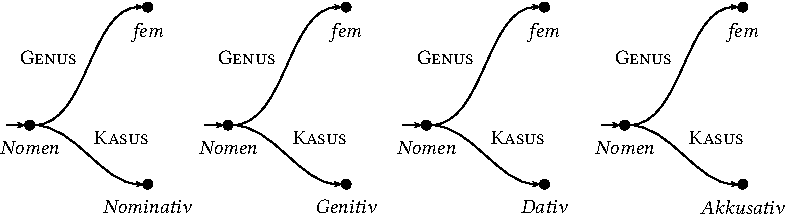
\includegraphics{Figures/frau-model-theoretic-crop}
}
% \oneline{%
% \begin{pspicture}(-0.5,0.4)(2.8,4.1)
% %\psgrid


%      \psset{fillstyle=solid, fillcolor=black,radius=0.75mm}
%      \pnode(-0.4,2){start1}
%      \Cnode(0,2){noun1}
%      \Cnode(2,4){fem1}
%      \Cnode(2,1){nom1}


%      \psset{fillstyle=none,nodesep=0pt,angleB=180,arrows=->} 

%      \nccurve{start1}{noun1}
%      \nccurve{noun1}{fem1}\naput{\textsc{genus}}
%      \nccurve{noun1}{nom1}\naput{\textsc{kasus}}

%      \nput{270}{noun1}{\type{noun}}
%      \nput{270}{fem1}{\type{fem}}
%      \nput{270}{nom1}{\type{Nominativ}}
% \end{pspicture}
% \begin{pspicture}(-0.5,0.4)(2.8,4.1)
% %\psgrid


%      \psset{fillstyle=solid, fillcolor=black,radius=0.75mm}
%      \pnode(-0.4,2){start2}
%      \Cnode(0,2){noun2}
%      \Cnode(2,4){fem2}
%      \Cnode(2,1){nom2}


%      \psset{fillstyle=none,nodesep=0pt,angleB=180,arrows=->} 

%      \nccurve{start2}{noun2}
%      \nccurve{noun2}{fem2}\naput{\textsc{genus}}
%      \nccurve{noun2}{nom2}\naput{\textsc{kasus}}

%      \nput{270}{noun2}{\type{noun}}
%      \nput{270}{fem2}{\type{fem}}
%      \nput{270}{nom2}{\type{Genitiv}}
% \end{pspicture}
% \begin{pspicture}(-0.5,0.4)(2.8,4.1)
% %\psgrid


%      \psset{fillstyle=solid, fillcolor=black,radius=0.75mm}
%      \pnode(-0.4,2){start2}
%      \Cnode(0,2){noun2}
%      \Cnode(2,4){fem2}
%      \Cnode(2,1){nom2}


%      \psset{fillstyle=none,nodesep=0pt,angleB=180,arrows=->} 

%      \nccurve{start2}{noun2}
%      \nccurve{noun2}{fem2}\naput{\textsc{genus}}
%      \nccurve{noun2}{nom2}\naput{\textsc{kasus}}

%      \nput{270}{noun2}{\type{noun}}
%      \nput{270}{fem2}{\type{fem}}
%      \nput{270}{nom2}{\type{Dativ}}
% \end{pspicture}
% \begin{pspicture}(-0.5,0.4)(2.8,4.1)
% %\psgrid


%      \psset{fillstyle=solid, fillcolor=black,radius=0.75mm}
%      \pnode(-0.4,2){start2}
%      \Cnode(0,2){noun2}
%      \Cnode(2,4){fem2}
%      \Cnode(2,1){nom2}


%      \psset{fillstyle=none,nodesep=0pt,angleB=180,arrows=->} 

%      \nccurve{start2}{noun2}
%      \nccurve{noun2}{fem2}\naput{\textsc{genus}}
%      \nccurve{noun2}{nom2}\naput{\textsc{kasus}}

%      \nput{270}{noun2}{\type{noun}}
%      \nput{270}{fem2}{\type{fem}}
%      \nput{270}{nom2}{\type{Akkusativ}}
% \end{pspicture}}
\caption{\label{abb-avm-frau}Merkmalstrukturen zur Beschreibung von \emph{Frau} in (\ref{avm-frau})}
\end{figure}
%-----------------------------------------------------------------------------
\begin{figure}
%\oneline{%
\centerline{%
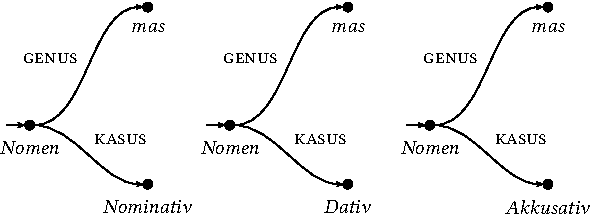
\includegraphics{Figures/mann-model-theoretic-crop}
}
% \begin{pspicture}(-0.5,0.4)(2.8,4.1)
% %\psgrid
% %
% %
%      \psset{fillstyle=solid, fillcolor=black,radius=0.75mm}
%      \pnode(-0.4,2){start1}
%      \Cnode(0,2){noun1}
%      \Cnode(2,4){mas1}
%      \Cnode(2,1){nom1}
% %
% %
%      \psset{fillstyle=none,nodesep=0pt,angleB=180,arrows=->} 
% %
%      \nccurve{start1}{noun1}
%      \nccurve{noun1}{mas1}\naput{\textsc{genus}}
%      \nccurve{noun1}{nom1}\naput{\textsc{kasus}}
% %
%      \nput{270}{noun1}{\type{noun}}
%      \nput{270}{mas1}{\type{mas}}
%      \nput{270}{nom1}{\type{Nominativ}}
% \end{pspicture}
% \begin{pspicture}(-0.5,0.4)(2.8,4.1)
% %\psgrid
% %
%      \psset{fillstyle=solid, fillcolor=black,radius=0.75mm}
%      \pnode(-0.4,2){start2}
%      \Cnode(0,2){noun2}
%      \Cnode(2,4){mas2}
%      \Cnode(2,1){nom2}
% %
% %
%      \psset{fillstyle=none,nodesep=0pt,angleB=180,arrows=->} 
% %
%      \nccurve{start2}{noun2}
%      \nccurve{noun2}{mas2}\naput{\textsc{genus}}
%      \nccurve{noun2}{nom2}\naput{\textsc{kasus}}
% %
%      \nput{270}{noun2}{\type{noun}}
%      \nput{270}{mas2}{\type{mas}}
%      \nput{270}{nom2}{\type{Dativ}}
% \end{pspicture}
% \begin{pspicture}(-0.5,0.4)(2.8,4.1)
% %\psgrid
% %
%      \psset{fillstyle=solid, fillcolor=black,radius=0.75mm}
%      \pnode(-0.4,2){start2}
%      \Cnode(0,2){noun2}
%      \Cnode(2,4){mas2}
%      \Cnode(2,1){nom2}
% %
% %
%      \psset{fillstyle=none,nodesep=0pt,angleB=180,arrows=->} 
% %
%      \nccurve{start2}{noun2}
%      \nccurve{noun2}{mas2}\naput{\textsc{genus}}
%      \nccurve{noun2}{nom2}\naput{\textsc{kasus}}
% %
%      \nput{270}{noun2}{\type{noun}}
%      \nput{270}{mas2}{\type{mas}}
%      \nput{270}{nom2}{\type{Akkusativ}}
% \end{pspicture}}
\caption{\label{abb-avm-mann}Merkmalstrukturen zur Beschreibung von \emph{Mann} in  (\ref{avm-mann})}
\end{figure}
In diesen Darstellungen gehört zu jedem Knoten ein Typ (\type{noun}, \type{fem}, \type{Nominativ},
\ldots), wobei die Typen in den Merkmalstrukturen immer maximal spezifisch sind, \dash keine
Untertypen mehr haben. Es gibt immer einen Eingangsknoten (im Beispiel \type{noun}), und die anderen
Knoten sind mit Pfeilen verbunden, an denen jeweils die Merkmalsnamen (\textsc{genus}, \textsc{kasus}) stehen.

Geht man noch einmal zum Personenbeispiel aus den vorigen Abschnitten zurück,
so kann man sich den Unterschied zwischen Modell und Beschreibung so verdeutlichen:
%\NOTE{JB: unklar, Vor allem der Begriff M-Beschreibung/beschreibt ist ihm nicht klar}
Wenn wir ein Modell von Personen haben, das Vorname, Nachname, Geburtstag,
Geschlecht und Haarfarbe enthält, dann ist es klar, dass jedes modellierte Objekt
einen Geburtstag hat, wir können aber in Beschreibungen die Angaben in Bezug
auf den Geburtstag weglassen, wenn diese bei der Formulierung von Beschränkungen
oder Suchen unwichtig sind.

Den Zusammenhang zwischen (linguistischen) Phänomenen, dem Modell
und der formalen Theorie verdeutlicht Abbildung~\vref{abb-modell}.
\begin{figure}[htbp]
\centerline{%
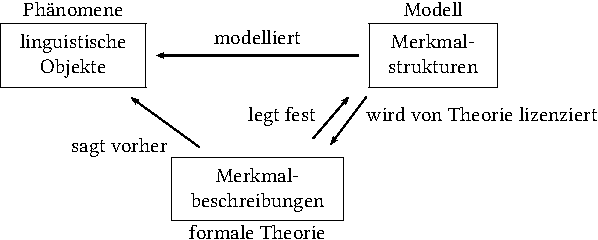
\includegraphics{Figures/model-theory-phenomenon-crop}
}
% %{
% \begin{pspicture}(0,0)(10.4,5)
% %\psgrid
% \rput[Bl](0,0){%
% \begin{tabular}[b]{@{}ccc@{}}
% Phänomen && Modell\\
% \rnode{phen}{\fbox{\begin{tabular}{c}
% Linguistische\\
% Objekte\\
% \end{tabular}}}&&\rnode{modell}{\fbox{\begin{tabular}{c}
% Merkmal-\\
% strukturen\\
% \end{tabular}}}\\[10ex]
% &\rnode{theorie}{\fbox{\begin{tabular}{c}
% Merkmal-\\
% beschreibungen\\
% \end{tabular}}}\\
% &Formale Theorie\\
% \end{tabular}}
% %\ncline{->}[l]{modell}[r]{phen}%
% \ncline{->}{modell}{phen}\nbput{modelliert}
% %\ncdiag[angleA=180,angleB=45]{->}{modell}{theorie}
% \psline{<-}(6.0,1.6)(6.6,2.6)
% \rput[Bl](6.6,2){wird von Theorie lizenziert} % früher Erfüllung, jetzt FR Änderung
% \psline{->}(5.175,1.7)(6.1,3.15)
% \rput[Bl](4.2,2.4){legt fest}
% %\nccurve{<-}{modell}{theorie}\nbput{legt fest}
% \ncline{->}{theorie}{phen}\naput{sagt vorher}%
% %\ncline{<->}[b]{modell}[tr]{theorie}%
% %\ncline{->}[tl]{theorie}[b]{phen}%
% \end{pspicture}
%\begin{pspicture}(0,0)(10.4,5)
%\psgrid
% \rput[Bl](0,0){%
% \begin{tabular}[b]{@{}ccc@{}}
% Phänomen && Modell\\
% \rnode{phen}{\fbox{\begin{tabular}{c}
% Linguistische\\
% Objekte\\
% \end{tabular}}}&&\rnode{modell}{\fbox{\begin{tabular}{c}
% Merkmal-\\
% strukturen\\
% \end{tabular}}}\\[10ex]
% &\rnode{theorie}{\fbox{\begin{tabular}{c}
% Merkmal-\\
% beschreibungen\\
% \end{tabular}}}\\
% &Formale Theorie\\
% \end{tabular}}
% %\anodeconnect[l]{modell}[r]{phen}%
% \ncline{->}{modell}{phen}\nbput{modelliert}
% %\ncdiag[angleA=180,angleB=45]{->}{modell}{theorie}
% \psline{<-}(6.0,1.6)(6.6,2.4)
% \rput[Bl](6.6,2){wird von Theorie lizenziert} % früher Erfüllung, jetzt FR Änderung
% \psline{->}(5.6,1.6)(6.2,2.4)
% \rput[Bl](4.5,2.4){legt fest}
% %\nccurve{<-}{modell}{theorie}\nbput{legt fest}
% \ncline{->}{theorie}{phen}\naput{sagt vorher}%
% %\aanodeconnect[b]{modell}[tr]{theorie}%
% %\anodeconnect[tl]{theorie}[b]{phen}%
% \end{pspicture}
\caption{\label{abb-modell}Phänomen, Modell und formale Theorie}
\end{figure}\nocite{Netter98a}%S. 26
%\NOTE{WS: zwischen Modell und Theorie sollten zwei Pfeile sein.}
% ###########
% zwei Pfeile: Beschreibung legt Modell fest , um Rekursion zu erfassen (beschreibt geht wohl auch, ist aber sloppy)
%
% Modell wird von der formalen Theorie lizenziert. 
%
% Phänomen + Modell -> PS: modelliert -> lassen wir so.
%
Das Modell modelliert linguistische Phänomene. Es muss außerdem
%alle Beschränkungen unserer Theorie erfüllen. 
von unserer Theorie lizenziert werden.
Die Theorie legt das Modell fest % FR: festlegen  gibt mehrere Modelle, exhaustive Modell enthält alle Sätze
und macht außerdem Vorhersagen in Bezug auf mögliche
Phänomene.

In den folgenden Kapiteln wird eine Theorie des Deutschen entwickelt.
Das bedeutet, dass geklärt wird, welche Merkmale zur Modellierung
von Sprache benötigt werden und welche Werte diese Merkmale im Deutschen haben
können. Die Theorie formuliert Beschränkungen über das Auf"|treten
bestimmter Werte bzw.\ die Gleichheit von Werten.
\is{Modell|)}\is{Theorie|)}\is{Phänomen|)}\is{Merkmalbeschreibung|)}\is{Merkmalstruktur|)}
%}{}


\questions{

\begin{enumerate}
\item Weshalb verwendet man in der HPSG Typen?
\item Sind die folgenden Strukturen jeweils kompatibel, \dash, können sie benutzt werden,
      um dasselbe Objekt zu beschreiben?
\ea
\onems{
vorname  \type{max}\\
nachname \type{meier}\\
vater     \ms[person]{
              vorname  & peter\\
              nachname & meier\\
             }\\
}\hspace{0.5cm}\onems{
vorname  \type{max}\\
nachname \type{meier}\\
vater    \ms[person]{
              vorname  & peter\\
              nachname & müller\\
             }\\
}
\z
%\tcbbreak
\ea
\onems{
vorname   \type{max}\\
nachname  \type{meier}\\
vater      \ms[person]{
              vorname  & peter\\
              nachname & meier\\
             }\\
}\hspace{0.5cm}\onems{
vorname   \type{max}\\
nachname  \type{meier}\\
mutter      \ms[person]{
              vorname  & ursula\\
              nachname & müller\\
             }\\
}
\z

\end{enumerate}
}


\exercises{

\begin{enumerate}
\item Überlegen Sie, wie man Musikinstrumente mittels Merkmalstrukturen beschreiben könnte.
\item\label{Übung-Listen} In diesem Kapitel wurden Listen eingeführt. Dies sieht wie eine Erweiterung des Formalismus
      aus. Dem ist aber nicht so, denn man kann die Listennotation in eine Notation überführen,
      die nur mit Merkmal"=Wert"=Paaren auskommt. Überlegen Sie, wie das geht.
\item (Zusatzaufgabe) Im folgenden Kapitel wird die Relation \emph{append}\is{Relation!\emph{append}} eine Rolle
      spielen, die dazu dient, zwei Listen zu einer dritten zu verknüpfen. Relationale
      Beschränkungen wie \emph{append} stellen eine Erweiterung des Formalismus dar. Mittels
      relationaler Beschränkungen kann man beliebige Werte von Merkmalen zu anderen Werten in
      Beziehung setzen, \dash, man kann kleine Programme schreiben, die einen Wert in Abhängigkeit von
      anderen Werten ausrechnen.  Es stellt sich die Frage, ob man solch mächtige Beschreibungsmittel in
      einer linguistischen Theorie braucht und wenn man sie zulässt, was für eine Komplexität man
      ihnen zubilligt. Eine Theorie, die ohne relationale Beschränkungen auskommt, ist einer anderen
      vorzuziehen (siehe auch Kapitel~\ref{sec-kriterien} zum Vergleich von Theorien).

      Für die Verkettung von Listen gibt es eine direkte Umsetzung in Merkmalstrukturen ohne
      relationale Beschränkungen. Finden Sie diese. Geben Sie Ihre Quellen an und dokumentieren Sie,
      wie Sie bei der Suche nach der Lösung vorgegangen sind.
\end{enumerate}
}


\furtherreading{

Dieses Kapitel sollte den Leser auf leicht verständliche Weise an getypte Merkmalbeschreibungen und -strukturen heranführen.
Mathematische Eigenschaften der Strukturen, der Typhierarchien und der Verknüpfungsmöglichkeiten
der Beschreibungen solcher Strukturen können hier nicht erörtert werden. Die Kenntnis zumindest eines Teils dieser Eigenschaften
sind aber für die Arbeit in der Computerlinguistik und auch beim Entwickeln eigener Analysen
wichtig. Der interessierte Leser sei deshalb auf die folgenden Publikationen verwiesen:
%
Das Buch von \citet{Shieber86a} ist eine kurze Einführung in die Theorie der
Unifikationsgrammatiken. Es wird ein ziemlich allgemeiner Überblick gegeben, 
und wichtige Grammatik-Typen (DCG\is{Definite Clause Grammar@\textit{Definite Clause Grammar\/} (DCG)}, 
\lfg, \gpsg, HPSG, PATR-II\is{PATR-II}) werden vorgestellt.
%
\citet{Johnson88}
beschreibt den Formalismus ungetypter Merkmalstrukturen mathematisch exakt.
%
\citet{Carpenter92a} setzt sich sehr mathematisch mit getypten Merkmalstrukturen auseinander.  Der
Formalismus, den \citet{King99a-u} für HPSG"=Grammatiken entwickelt hat, bildet die Grundlage für
den von \citet{Richter2004a-u} entwickelten Formalismus, der derzeit als Standard
gilt. \citet{Richter2024a} fasst verschiedene Ansätze bzgl.\ formaler Grundlagen in der HPSG zusammen
und gibt einen Überblick über aktuell gültige Grundannahmen.

}

% FR: auch Pollard99 strong generative capacity. ist Variante auf Kings Modelltheorie


%      <!-- Local IspellDict: de -->


%% -*- coding:utf-8 -*-
%%%%%%%%%%%%%%%%%%%%%%%%%%%%%%%%%%%%%%%%%%%%%%%%%%%%%%%%%
%%   $RCSfile: 3-hpsg-valenz-psg.tex,v $
%%  $Revision: 1.17 $
%%      $Date: 2008/09/30 09:14:41 $
%%     Author: Stefan Mueller (CL Uni-Bremen)
%%    Purpose: 
%%   Language: LaTeX
%%%%%%%%%%%%%%%%%%%%%%%%%%%%%%%%%%%%%%%%%%%%%%%%%%%%%%%%%

\chapter{Valenz und Grammatikregeln}
\label{Kapitel-Valenz}

%% \NOTE{
%% Haitao Liu:
%% A small note: the title of the third chapter is "`Valenz unu and
%% Grammatikregeln"'. I can understand there the term "`valence"' should lie
%% within the framework of HPSG, but it seems to me if you can mention 2 or
%% 3 important documents of valency theory outside HPSG, it is helpful to
%% the readers. Why I hope to see that, because there are many documents in
%% German about valency theory, it is good if we could link the term to
%% traditional use of the term. I have noted that in the reference already
%% is the name of Helbig's valency dictionary. 
%% }
In diesem Kapitel geht es um die Interaktion zwischen Grammatikregeln und Valenzinformation.
Der Begriff der Valenz stammt aus der Chemie. Atome können sich mit anderen Atomen
zu mehr oder weniger stabilen Molekülen verbinden. Wichtig für die Stabilität ist, wie
Elektronenschalen besetzt sind. Eine Verbindung mit anderen Atomen kann dazu führen,
dass eine Elektronenschale voll besetzt ist, was dann zu einer stabilen Verbindung führt.
%\footnote{
%\url{http://www.quantenwelt.de/atomphysik/modelle/bindungen/valenz.html}.
%\url{http://www.iap.uni-bonn.de/P2K/periodic_table/valences.html}. \urlchecked{09}{11}{2006}.%
%}
Die Valenz\is{Valenz|(} sagt etwas über die Anzahl der Wasserstoffatome aus,
die mit einem Atom eines Elements verbunden werden können. In der Verbindung H$_2$O
hat Sauerstoff die Valenz 2. Man kann nun die Elemente in Valenzklassen einteilen.
Elemente mit einer bestimmten Valenz werden im Periodensystem von Mendeleev
in einer Spalte repräsentiert.

Dieses Konzept wurde von \citet{Tesniere59a-u}\nocite{Tesniere80a-u}
auf die Linguistik übertragen: Ein Kopf braucht bestimmte Argumente,
um eine stabile Verbindung einzugehen. Wörter mit der gleichen Valenz -- also mit der gleichen
Anzahl und Art von Argumenten\is{Argument} -- werden in Valenzklassen eingeordnet, da sie sich in Bezug
auf die Verbindungen, die sie eingehen, gleich verhalten. Abbildung~\vref{abb-chemie-valenz}
zeigt Beispiele aus der Chemie und der Linguistik.
\begin{figure}
\centerline{
\begin{forest}
[O
  [H] 
  [H] ]
\end{forest}
\hspace{5em}
\begin{forest}
[helfen
 [Aicke]
 [Conny] ]
\end{forest}
}
\caption{\label{abb-chemie-valenz}Verbindung von Sauerstoff mit Wasserstoff und Verbindung
eines Verbs mit seinen Argumenten}
\end{figure}

Weitere Information zum Valenzbegriff in der Linguistik findet man in
\citew{AEEHHL2003a-ed,AEEHHL2006a-ed}. Das Buch von Tesnière wurde 1980 in Teilen ins Deutsch
übersetzt \citep{Tesniere80a-u}. Seit 2015 ist eine vollständige Übersetzung ins Englische verfügbar \citep{Tesniere2015a-u}.

Im folgenden wird gezeigt, wie Valenzinformation so repräsentiert werden kann,
dass man statt vieler spezifischer Phrasenstrukturregeln ganz allgemeine Schemata 
zur Lizenzierung syntaktischer Strukturen verwenden kann.

\section{Repräsentation von Valenzinformation}

Die in Kapitel~\ref{sec-psg} diskutierten Phrasenstrukturgrammatiken\is{Phrasenstrukturgrammatik}
haben den Nachteil, dass man sehr viele Regeln für die verschiedenen Valenzmuster
braucht. (\mex{1}) zeigt beispielhaft einige solche Regeln und die
dazugehörigen Verben.
\ea
\label{psg-valenz}
\begin{tabular}[t]{l@{~$\to$~}l@{\hspace{4em}}l}
      S & NP, V                             & \emph{X schläft}\\
      S & NP, NP, V                         & \emph{X Y erwartet}\\
      S & NP, PP[\textit{über\/}], V           & \emph{X über Y spricht}\\
      S & NP, NP, NP, V                     & \emph{X Y Z gibt}\\
      S & NP, NP, PP[\textit{mit\/}], V        & \emph{X Y mit Z dient}\\
      \end{tabular}
\z
Damit die Grammatik keine falschen Sätze erzeugt, muss man dafür sorgen, 
dass Verben nur mit passenden Regeln verwendet werden können.
\eal
\ex[*]{
dass Kirby das Buch schläft
}
\ex[*]{
dass Kirby erwartet
}
\ex[*]{
dass Kirby über den Mann erwartet 
}
\zl
Man muss also Verben (allgemein Köpfe) in Valenzklassen einordnen. Diese
Valenzklassen müssen den Grammatikregeln zugeordnet sein. Damit
ist die Valenz doppelt kodiert: Zum einen sagt man in den Regeln etwas
darüber aus, welche Elemente zusammen vorkommen müssen/""können,
und zum anderen ist Valenzinformation im Lexikon enthalten.

Um solcherart redundante Repräsentation zu vermeiden, nimmt
man in der HPSG -- wie in der Kategorialgrammatik\is{Kategorialgrammatik (CG)} -- Beschreibungen der Argumente eines
Kopfes in die lexikalische Repräsentation des Kopfes auf. 

Ein weiteres Argument dafür, dass Valenzinformation im Lexikon verfügbar sein muss, ist, dass
bestimmte morphologische Prozesse Bezug auf Valenzinformation nehmen. So ist zum Beispiel die \bard
nur für Verben produktiv verwendbar, die ein Akkusativobjekt verlangen: \emph{unterstützbar} ist
bildbar, \noword{helfbar} dagegen nicht.  

In der Beschreibung von Köpfen gibt es verschiedene Valenzmerkmale (\textsc{spr} für Spezifikatoren und \textsc{comps}
für Komplemente). Diese enthalten Beschreibungen
der Objekte, die mit einem Kopf kombiniert werden müssen, damit eine
vollständige Phrase vorliegt. Vorerst ist nur der \compsw wichtig. (\mex{1}) zeigt Beispiele für die Verben aus (\mex{-1}):
\ea
\begin{tabular}[t]{@{}lll}
      Verb             & \comps\\
      \emph{schlafen} & \sliste{ NP }\\
      \emph{erwarten} & \sliste{ NP, NP }\\
      \emph{sprechen} & \sliste{ NP, PP[\type{über}] }\\
      \emph{geben}    & \sliste{ NP, NP, NP }\\
      \emph{dienen}   & \sliste{ NP, NP, PP[\type{mit}] }\\  
      \end{tabular}
\z
Man spricht auch davon, dass ein bestimmter Kopf für bestimmte Argumente
subkategorisiert\is{Subkategorisierung} ist. Diese Redeweise kommt wohl daher, dass die Köpfe
bezüglich ihrer Wortart bereits kategorisiert sind und dann durch die Valenzinformation weitere
Unterklassen (wie \zb intransitives oder transitives Verb)  
%\glossary{name={intransitives Verb},description={Intransitive Verben können im Gegensatz zu transitiven Verben kein Akkusativobjekt binden bzw. benötigen zusätzlich eine Präposition.}}
gebildet werden. Im Englischen gibt es auch die Verwendung \emph{X subcategorizes for Y}, was soviel wie
\emph{X verlangt Y} oder \emph{X selegiert Y}\is{Selektion} heißt. Man sagt auch, dass X Y
\emph{regiert}.\is{Rektion}
Früher hieß das Valenzmerkmal auch \subcat für Subkategorisierung.
% Rektion schließt in der Dependenzgrammatik auch Adjunkte ein. Das ist also vielleicht etwas
% irreführend, aber irgendwo muss Rektion noch erwähnt werden.

Statt spezifische Regeln wie die in (\ref{psg-valenz}) zu verwenden, kann man Regelschemata wie die in (\mex{1})
für Kopf"=Argument"=Kombination benutzen:
\ea
\label{psg-regeln-append}
\begin{tabular}[t]{@{}l@{~}l@{~$\to$~}l}
a.& V[\comps \ibox{1}] &  \ibox{2}, V[\comps \ibox{1} $\oplus$ \sliste{ \ibox{2} } ]\\
b.& A[\comps \ibox{1}] &  \ibox{2}, A[\comps \ibox{1} $\oplus$ \sliste{ \ibox{2} } ]\\
c.& N[\comps \ibox{1}] &  \ibox{2}, N[\comps \ibox{1} $\oplus$ \sliste{ \ibox{2} } ]\\
d.& P[\comps \ibox{1}] &  P[\comps \ibox{1} $\oplus$ \sliste{ \ibox{2} } ], \ibox{2}\\
\end{tabular}
\z
% In den Boxen verwende ich \emph{A} und \emph{B} statt 1 oder 2, damit man nicht mit den
% Strukturteilungen in den folgenden Abbildungen durcheinanderkommt.

Die Schemata lizenzieren die Verbindung von V, A, N bzw.\ P mit einem Element aus der
\compsl.
Dabei ist `$\oplus$'\is{$\oplus$} (\emph{append}\is{Relation!\emph{append}}) eine Relation zur Verknüpfung zweier Listen:\\
\ea
\begin{tabular}[t]{@{}l@{~}l@{}}
\phonliste{ x, y } = & \phonliste{ x } $\oplus$ \phonliste{ y } oder\\
                     & \phonliste{} $\oplus$ \phonliste{ x, y } oder\\
                     & \phonliste{ x, y } $\oplus$ \phonliste{}\\
\end{tabular}
\z
Die Anwendung der Regel (\mex{-1}a) soll anhand der Beispiele in (\mex{1}) erklärt werden:
\eal
\ex dass Aicke schläft
\ex\label{bsp-weil-peter-maria-erwartet}
dass Aicke Conny erwartet
\zl
Die \compsl im Lexikoneintrag von \emph{schläft} enthält genau eine NP. Setzt man
den Lexikoneintrag für \emph{schläft} in die Regel in (\ref{psg-regeln-append}a) ein,
ergibt sich (\mex{1}):
\ea
\label{ex-Regel-mit-einer-NP-in-Valenz}
V[\comps \ibox{1}] $\to$ \ibox{2} NP, V[\comps \ibox{1} \sliste{} $\oplus$ \sliste{ \ibox{2} NP } ]
\z
\emph{append} teilt die \compsl von \emph{schläft} in zwei Teile. 
Ein Teil ist eine einelementige Liste, die die NP enthält, der zweite Teil ist die leere Liste. 
Die leere Liste entspricht der Liste der noch zu sättigenden Argumente.
Abbildung~\vref{fig-Aicke-schlaeft} zeigt den durch das Regelschema lizenzierten Baum.
\begin{figure}
\centerline{
\begin{forest}
sm edges
[{V[\comps \sliste{}]}
  [{\ibox{1} NP[\type{nom}]}
    [Aicke]]
  [{V[\comps \sliste{ \ibox{1} }]}
    [schläft]]]
\end{forest}}
%
\caption{\label{fig-Aicke-schlaeft}Analyse für \emph{Aicke schläft}}
\end{figure}

Lässt man die Ausdrücke in eckigen Klammern in (\mex{0}) weg, bleibt nur (\mex{1}) übrig.
\ea
V $\to$ NP, V
\z
Obwohl die Regel in (\mex{0}) genauso aussieht wie die Phrasenstrukturregeln, die
wir im Kapitel~\ref{sec-psg} behandelt haben, ist sie anderer Natur:
Die Information darüber, dass ein Verb mit einer NP kombiniert wird, wird nicht in
den Regeln spezifiziert, sondern wird über die \comps{}"=Information durch das Verb
beigesteuert.

Die \compsl im Lexikoneintrag von \emph{erwartet} enthält genau zwei NPen. Setzt man
den Lexikoneintrag für \emph{erwartet} in die erste Regel in (\ref{psg-regeln-append}) ein,
ergibt sich (\mex{1}):
\ea
V[\comps \ibox{1}] $\to$ \ibox{2} NP, V[\comps \ibox{1} \sliste{ NP } $\oplus$ \sliste{ \ibox{2} NP } ]
\z
Das Ergebnis der Regelanwendung ist V[\comps \sliste{ NP }]. Das entspricht dem
Lexikoneintrag von \emph{schläft}. Die Regel kann also wie in (\ref{ex-Regel-mit-einer-NP-in-Valenz}) noch einmal
angewendet werden, so dass man dann eine vollständig gesättigte Phrase bekommt. Das zeigt
Abbildung~\vref{fig-Aicke-Conny-erwartet}.

%\psset{xunit=1cm,yunit=5.4mm}
\begin{figure}
\centerline{%
\begin{forest}
sm edges
[{V[\comps \sliste{}]}
  [{\ibox{1} NP[\type{nom}]}
    [Aicke]]
  [{V[\comps \sliste{ \ibox{1} }] }
    [{\ibox{2} NP[\type{acc}]} 
      [Conny]]
    [{V[\comps \sliste{ \ibox{1}, \ibox{2} }] }
      [erwartet]]]]
\end{forest}}
\caption{\label{fig-Aicke-Conny-erwartet}Analyse für \emph{Aicke Conny erwartet}}
\end{figure}

Die Regeln in (\ref{psg-regeln-append}) kann man nun auf zweierlei Weise verallgemeinern:
Zuerst kann man von der Abfolge der Konstituenten auf der rechten Regelseite abstrahieren
(dazu später noch mehr). Man erhält dann (\mex{1}):
\ea
\label{abstraktion-linearisierung}
      \begin{tabular}[t]{@{}lll}
      V[\comps \ibox{1}] & $\to$ & V[\comps \ibox{1} $\oplus$ \sliste{ \ibox{2} } ] \ibox{2}\\
      N[\comps \ibox{1}] & $\to$ & N[\comps \ibox{1} $\oplus$ \sliste{ \ibox{2} } ] \ibox{2}\\
      A[\comps \ibox{1}] & $\to$ & A[\comps \ibox{1} $\oplus$ \sliste{ \ibox{2} } ] \ibox{2}\\
      P[\comps \ibox{1}] & $\to$ & P[\comps \ibox{1} $\oplus$ \sliste{ \ibox{2} } ] \ibox{2}\\
      \end{tabular}
\z
In einem zweiten Schritt kann man, wie das in den \xbar-Schemata gemacht wurde, über
die Kategorie des Kopfes abstrahieren. Man erhält dann ein abstraktes Schema, das
die Regeln in (\ref{psg-regeln-append}) bzw.\ in (\mex{0}) zusammenfasst:
\ea
\label{regelschema-psg-comps}
\begin{tabular}[t]{@{}lll}
H[\comps \ibox{1}] & $\to$ & H[\comps \ibox{1} $\oplus$ \sliste{ \ibox{2} } ] \ibox{2}\\
\end{tabular}
\z
`H' steht hierbei für irgendeinen Kopf (also \zb A, N, P oder V).
%% Zwei mögliche Instantiierungen dieses Schemas zeigt (\mex{1}):
%% \ea
%% \begin{tabular}[t]{@{}lll}
%% N[\comps \ibox{1}] & $\to$ & Det N[\comps \ibox{1} $\oplus$ \sliste{ Det } ]\\
%% V[\comps \ibox{1}] & $\to$ & V[\comps \ibox{1} $\oplus$ \sliste{ NP } ]~~ NP\
%% \end{tabular}
%% \z

Nach diesen Vorbemerkungen zur Repräsentation von Valenzinformation können wir uns nun
dem Aufbau von Lexikoneinträgen zuwenden: Lexikoneinträge werden immer durch Merkmalstrukturen modelliert. Information über die
Aussprache (\textsc{phonology}\isfeat{phon}), die Wortart (\textsc{part-of-speech}, \textsc{p-o-s}) und die Valenz
(hier vorerst nur \comps)\isfeat{comps} kann wie folgt dargestellt werden:
\ea
\label{le-gibt-1}
\textit{gibt\/} (finite Form):\\
\ms[word]{ 
     phon   & \phonliste{ gibt } \\
     p-o-s  & verb\\
     comps & \liste{ NP[\type{nom}], NP[\type{dat}], NP[\type{acc}]   } \\
}
\z
Als Wert von \phon müssten phonologische Umschriften der Wörter angegeben werden,
was oft der Einfachheit halber nicht gemacht wird.
Statt dessen verwendet man die orthographische Form. Zur Behandlung der Phonologie in HPSG siehe
\citew{BK94b} und \citew{Hoehle99a-u}.

NP[\type{nom}], NP[\type{dat}] und NP[\type{acc}] stehen für komplexe Merkmalstrukturen, die intern
genauso aufgebaut sind wie der Eintrag für \emph{gibt} in (\mex{0}). Wie die Kasusinformation
repräsentiert wird, wird auf Seite~\pageref{page-ref-case-feat} erklärt. Die Reihenfolge der
Elemente entspricht der unmarkierten Reihenfolge\label{page-unmarkierte-Reihenfolge}, \dash der Reihenfolge, die man in den meisten
Äußerungskontexten verwenden kann und die intonatorisch unmarkiert ist \citep{Hoehle82a}. Bei dreistelligen Verben ist
das meistens die Reihenfolge \type{nom}, \type{dat}, \type{acc}, aber bei Verben wie
\emph{aussetzen} ist die Reihenfolge \type{acc} vor \type{dat} die unmarkierte \parencites[\page 249]{Wegener85b}[S.\,60]{Hoberg81a}. 
%
% Die Reihenfolge der Elemente in der \compsl entspricht der Obliqueness"=Hierarchie\is{Obliqueness}
% von \citet{KC77a} und \citet{Pullum77a}:
% \begin{table}[H]
% \resizebox{\linewidth}{!}{%
% \begin{tabular}{@{}l@{\hspace{1ex}}l@{\hspace{1ex}}l@{\hspace{1ex}}l@{\hspace{1ex}}l@{\hspace{1ex}}l@{}}
% SUBJECT $=>$ & DIRECT $=>$ & INDIRECT $=>$ & OBLIQUES $=>$ & GENITIVES $=>$  & OBJECTS OF \\
%              & OBJECT      & OBJECT        &               &                 & COMPARISON 
% \end{tabular}%
% }\label{page-obliquen-h}
% \end{table}
% \noindent
% Diese Hierarchie gibt die unterschiedliche syntaktische Aktivität der grammatischen Funktion wieder.
% Elemente, die weiter links stehen, kommen eher in bestimmten syntaktischen Konstruktionen vor. Beispiele
% für syntaktische Konstruktionen, in denen Obliqueness eine Rolle spielt, sind:
% \begin{itemize}
% \item Ellipse\is{Ellipse} \citep{Klein85}
% \item Vorfeldellipse\is{Vorfeldellipse} \citep{Fries88b}
% \item freie Relativsätze\is{Relativsatz!freier}
%       \citep{Bausewein90,Pittner95b,Mueller99b}
% \item Passiv\is{Passiv} \citep{KC77a}
% \item Zustandsprädikate\is{Zustandsprädikat} \citep{Mueller2001c,Mueller2002b,Mueller2008a}
% \item Bindungstheorie\is{Bindungstheorie} (\citealp{Grewendorf85a}; \citealp{PS92a,ps2})
% \end{itemize}

% \noindent
% Eine Alternative für die Anordnung der Elemente in der \compsl wäre die Abfolge 
% NP[\textit{nom\/}], NP[\textit{dat}], NP[\textit{acc}], die ebenfalls bei vielen Phänomenen eine Rolle spielt. 
% Ein Beispiel für ein solches Phänomen ist die Konstituentenstellung. Diese ist im Deutschen relativ frei. Statt (\mex{1}a) kann
% man in bestimmten Kontexten auch (\mex{1}b) äußern:
% \eal
% \ex weil der Mann der Frau das Buch gibt
% \ex weil der Mann das Buch der Frau gibt
% \zl
% Die Anzahl der Kontexte, in denen (\mex{0}b) geäußert werden kann, ist jedoch kleiner
% als die, in denen (\mex{0}a) geäußert werden kann. Man bezeichnet die Abfolge in (\mex{0}a)
% deshalb auch als präferierte Abfolge oder als Normalabfolge\is{Normalabfolge} \citep{Hoehle82a}.

% In der Literatur wird mitunter von einer größeren Verbnähe des Akkusativs\is{Kasus!Akkusativ} gesprochen,
% und es wird behauptet, dass eine Voranstellung des Verbs mit einem Dativ\is{Kasus!Dativ} nicht möglich
% ist (\citealt{Haftka81a}; \citealt{Haider82}; \citealt{Wegener90}; \citealt{Zifonun92a}).
% Zu dieser Behauptung gibt es Gegenbeispiele bei \citet{Uszkoreit87a}, \citet{SS88a}, %zitieren Thiersch82a-u
% \citet{Oppenrieder91a}, \citet{Grewendorf93} und G.\ \citet[\page5]{GMueller98a}.
% (\mex{1}) zeigt Korpusbelege, in denen ein Dativobjekt, das normalerweise vor dem Akkusativ
% angeordnet werden würde, zusammen mit einem infiniten Verb vorangestellt wurde:

% \eal
% \label{bsp-syntax-pvp-besonders}
% \ex Besonders Einsteigern empfehlen möchte ich Quarterdeck Mosaic, dessen gelungene grafische 
%     Oberfläche und Benutzerführung auf angenehme Weise über die ersten Hürden 
%     hinweghilft, obwohl sich die Funktionalität auch nicht zu verstecken braucht.\footnote{
%       c't, 9/95, S.\,156.}
% \ex Der Nachwelt hinterlassen hat sie eine aufgeschlagene \textit{Hör zu\/} und einen kurzen
%     Abschiedsbrief: \ldots\footnote{
%       taz, 18.11.98, S.\,20.}
% \zl
% Man könnte annehmen, dass der Dativ nur bei bestimmten Verben zusammen mit dem Verb vorangestellt
% werden kann und dass bei solchen Verben dafür der Akkusativ nicht mit dem Verb gemeinsam
% voranstellbar ist. Man würde also für einige Verben die Hierarchie SU $>$ DO $>$ IO und für andere
% SU $>$ IO $>$ DO annehmen. Die Beispiele in (\mex{1}) zeigen jedoch, dass mit demselben Verb Dativ +
% V und Akkusativ + V vorangestellt werden können.
% \eal
% \label{bsp-acc-dat-pvp}
% \ex Den Wählern erzählen sollte man diese Geschichte nicht.
% \ex Märchen erzählen sollte man den Wählern nicht.
% \zl

\section{Spezifikatoren}
\label{Abschnitt-SPR-Merkmal}

Wir haben bisher nur das Valenzmerkmal \comps benutzt. Es gibt 
noch das Merkmal \spr, das für die Repräsentation von Spezifikatoren verwendet wird. Für das Deutsche spielt \spr in Nominalstrukturen eine
Rolle. Ein Nomen wie \emph{Schwester} selegiert seinen Determinator über das \sprm. Komplemente, wie
sie bei relationalen Nomina wie \emph{Schwester}, \emph{Bild} oder Nominalisierungen wie \emph{Vorlesen} möglich sind, werden über \comps
selegiert. Abbildung~\ref{fig-die-Tochter-eines-Mitarbeiters} zeigt die Analyse von (\mex{1}a):
\eal
\ex die Tochter eines Mitarbeiters
\ex das Bild vom Gleimtunnel
\ex das Vorlesen von Büchern
\zl 
\begin{figure}
\centerfit{%
\begin{forest}
sm edges
[{N[\spr \eliste, \comps \eliste]}
   [Det [die] ]
   [N\feattab{
      \spr \nliste{ Det }, \comps \sliste{}}
     [N\feattab{
         \spr \nliste{ Det },\\
         \comps \nliste{ NP[\type{gen}] }} [Tochter] ]
        [{NP[\type{gen}]} [eines Mitarbeiters,roof] ] ] ]
\end{forest}}
\caption{\label{fig-die-Tochter-eines-Mitarbeiters}Analyse des Beispiels \emph{die Tochter eines Mitarbeiters}}
\end{figure}

Für die Analyse von Spezifikator-Kopf-Strukturen braucht man ein Schema, das analog zu dem in
(\ref{regelschema-psg-comps}) ist. Eine vorläufige Version ist in (\mex{1}) zu sehen:
\ea
\label{regelschema-psg-spr}
\begin{tabular}[t]{@{}lll}
H[\spr \ibox{1}] & $\to$ & \ibox{2}~~~ H[\spr \ibox{1}  $\oplus$ \sliste{ \ibox{2} }  ]\\
\end{tabular}
\z
Wir werden darauf im nächsten Kapitel zurückkommen.

Das Deutsche zählt typologisch zu den Subjekt-Objekt-Verb-Sprachen (SOV), so wie \zb auch Afrikaans,
Niederländisch, Japanisch, Koreanisch und Persisch. Das Englische, die skandinavischen Sprachen und die
romanischen Sprachen werden zu den Subjekt"=Verb"=Objekt"=Sprachen (SVO) gezählt. Ich habe in diesem Kapitel
alle Argumente von finiten Verben gleich behandelt. Sie sind alle in der \compsl repräsentiert. Das
ist berechtigt, weil Subjekte im Deutschen keinen besonderen Status haben, ja, es muss nicht mal
ein Subjekt im Satz geben. Das wird im kommenden Abschnitt genauer besprochen. Bei den SVO-Sprachen
ist das jedoch anders: Schon durch die Stellung hat das Subjekt einen anderen Status. Subjekte
stehen links vom Verb, andere Argumente rechts. Das wird in HPSG-Grammatiken dadurch erfasst, dass
für Subjekte ein separates Valenzmerkmal verwendet wird. In manchen Grammatiken ist das das \subjm,
in anderen das \sprm. Da ich das \subjm anders verwende, benutze ich wie \citet*[Kapitel~4.3]{SWB2003a} das \sprm
für die Repräsentation des Subjekts in SVO-Sprachen \citep[Kapitel~4.3]{MuellerGermanic}.

Die Struktur in Abbildung~\ref{fig-Aicke-expects-Conny} ist das Gegenstück zu
Abbildung~\ref{fig-Aicke-Conny-erwartet}. Die Komplemente stehen im Englischen rechts des Verbs, das
Subjekt steht links. Für das Subjekt gibt es eine besondere Position. Im Deutschen ist das nicht der
Fall. Da kann das Subjekt irgendwo stehen, Hauptsache, es steht links des Verbs. Gemeinsam mit den
anderen Argumenten.
\begin{figure}
\centerfit{%
\begin{forest}
sm edges
[{V[\spr \eliste, \comps \eliste]}
   [{NP[\type{nom}]} [Aicke] ]
   [V\feattab{
      \spr \sliste{ NP[\type{nom}] }, \comps \sliste{}}
     [V\feattab{
         \spr \sliste{ NP[\type{nom}] },\\
         \comps \sliste{ NP[\type{acc}] }} [expects] ]
        [{NP[\type{acc}]} [Conny] ] ] ]
\end{forest}}
\caption{\label{fig-Aicke-expects-Conny}Analyse des Beispiels \emph{Aicke expects Conny} in der
  SVO-Sprache Englisch}
\end{figure}



\section{Die Argumentstruktur}
\label{sec-argst-Liste}

Will man erfassen, was alle Sprachen (oder zumindest viele Sprachen) gemeinsam haben, ist es
sinnvoll, eine zugrundeliegende Struktur anzunehmen: die Argumentstruktur (\argst). Die Argumentstruktur ist
eine Liste, in der alle Argumente eines Kopfes enthalten sind. Diese Argumente werden dann auf die
Valenzmerkmale des jeweiligen Kopfes verteilt. Für das Englische kommt das Subjekt in die \sprl und
die Komplemente auf \comps. Für das Deutsche bleibt die \sprl finiter Verben leer und alle Argumente
kommen auf \comps. (\mex{1}) und (\mex{2}) zeigen prototypische Verben im Englischen und im Deutschen:

\ea
\label{ex-spr-comps-arg-st-Englisch}
\begin{tabular}[t]{@{}ll@{~~}l@{~~}l@{}}
Verb          & \spr                      & \comps                                     & \argst\\
\emph{sleep}  & \sliste{ NP[\type{nom}] } & \sliste{}                                  & \sliste{ NP[\type{nom}] }\\
\emph{expect} & \sliste{ NP[\type{nom}] } & \sliste{ NP[\type{acc}] }                  & \sliste{ NP[\type{nom}], NP[\type{acc}] }\\
\emph{speak}  & \sliste{ NP[\type{nom}] } & \sliste{ PP[\type{about}] }                & \sliste{ NP[\type{nom}], PP[\type{about}] }\\
\emph{give}   & \sliste{ NP[\type{nom}] } & \sliste{ NP[\type{acc}], NP[\type{acc}] }  & \sliste{ NP[\type{nom}], NP[\type{acc}], NP[\type{acc}] }\\
\emph{serve}  & \sliste{ NP[\type{nom}] } & \sliste{ NP[\type{acc}], PP[\type{with}] } & \sliste{ NP[\type{nom}], NP[\type{acc}], PP[\type{with}] }\\  
\end{tabular}
\z

\ea
\label{ex-spr-comps-arg-st-Deutsch}
\begin{tabular}[t]{@{}ll@{~~}l@{~~}l@{}}
Verb            & \spr                      & \comps                                      & \argst\\
\emph{schlafen}  & \sliste{ } & \sliste{ NP[\type{nom}] }                                  & \sliste{ NP[\type{nom}] }\\
\emph{erwarten} & \sliste{ } & \sliste{ NP[\type{nom}], NP[\type{acc}] }                  & \sliste{ NP[\type{nom}], NP[\type{acc}] }\\
\emph{sprechen} & \sliste{ } & \sliste{ NP[\type{nom}], PP[\type{über}] }                 & \sliste{ NP[\type{nom}], PP[\type{about}] }\\
\emph{geben}    & \sliste{ } & \sliste{ NP[\type{nom}], NP[\type{dat}], NP[\type{acc}] }  & \sliste{ NP[\type{nom}], NP[\type{dat}], NP[\type{acc}] }\\
\emph{dienen}   & \sliste{ } & \sliste{ NP[\type{nom}], NP[\type{dat}], PP[\type{with}] } & \sliste{ NP[\type{nom}], NP[\type{dat}], PP[\type{with}] }\\  
\end{tabular}
\z

In der Literatur findet man das Argumentrealisierungsprinzip, das für die Verteilung von Argumenten
auf Valenzlisten sorgt.
\ea
\label{Prinzip-Argumentrealisierung-einfach}%
Argumentrealisierungsprinzip\is{Prinzip!Argumentrealisierungs-} (vereinfachte Version):\\
\type{word} \impl
\avm{
[spr    & \1\\
 comps  & \2\\
 arg-st & \1 \+ \2]
}
\z
Die Formalisierung dieses Prinzips scheint einfach zu sein: Die \argstl wird in zwei Teile geteilt
und der erste Teil bildet die \sprl und der zweite die \compsl. Für das Deutsche kann man dann
für Verben einfach sagen, dass die \sprl die leere Liste ist. Es gibt aber – je nach Analyse – noch andere Phänomene,
die mit der Verteilung der Argumente auf Valenzlisten interagieren. \citet[\page 171]{GSag2000a-u} analysieren
die Voranstellung von Konstituenten (siehe Kapitel~\ref{Kapitel-nla}) so, dass die vorangestellten Konstituenten nicht mehr in den
Valenzmerkmalen auftauchen. Das muss dann im Argumentrealisierungsprinzip berücksichtigt
werden. Auch muss irgendwo geregelt werden, wie viele Elemente überhaupt in der \sprl vorkommen
können. Ohne eine solche Beschränkung könnten im Prinzip alle Elemente aus der \argstl in der \sprl
stehen und keins in der \compsl. Das alles soll uns hier nicht kümmern: Für deutsche Verben
ist die \sprl leer und alle Argumente finiter Verben werden unter \comps aufgeführt. Im folgenden
Abschnitt gebe ich einfach die Valenzmerkmale \spr und \comps an. Ich komme auf die von \argst
ausgehende Verteilung der Valenzinformation im Kapitel~\ref{Kapitel-Lexikon} über das Lexikon noch einmal zurück.

Die einheitliche \argstl hat den Vorteil, dass bestimmte Eigenschaften von Sprachen sprachübergreifend
gleich behandelt werden können. So kann zum Beispiel die Beziehung zwischen Syntax und Semantik (das
so genannte Linking\is{Linking}) auf \argst gemacht werden \citep*{DKW2024a}. Wir werden uns das im Kapitel~\ref{Kapitel-Semantik}
über Semantik genauer ansehen. Die Argumentstrukturliste ist für die Kasusvergabe (siehe Kapitel~\ref{Kapitel-Kasus})
und für die Bindungstheorie relevant.
\is{Valenz|)}
  
\section{Adjunkte}
\label{sec-Adjunkte-psg}

In den vorigen Abschnitten wurden die Argumente von Köpfen behandelt, in diesem Abschnitt sollen
Adjunkte besprochen werden. Auf S.\,\pageref{adj-kriterien} wurde festgehalten: Adjunkte füllen keine semantische
Rolle, Adjunkte sind iterierbar und Adjunkte sind optional. Argumente hingegen können eine
semantische Rolle ihres Kopfes füllen, der Kopf bestimmt normalerweise die Eigenschaften seiner
Argumente, zum Beispiel deren Kasus, und legt fest, wie viele Argumente er braucht. Für die
Argumente haben wir Valenzlisten verwendet. Für Adjunkte wäre das nicht sinnvoll. Im
Kapitel~\ref{sec-intro-arg-adj}\is{Adjunkt|(}\is{Modifikator|(} wurde festgestellt, dass die Form
von Adjunkten, die mit bestimmten Köpfen vorkommen können, relativ wenig beschränkt ist. Andererseits
können Adjunkte oft nur mit Köpfen einer bestimmten Wortart vorkommen. Flektierte
Adjektive sind \zb nur als Modifikatoren von Nomina möglich. 
\eal
\ex[]{
der laute Gesang
}
\ex[*]{
Aicke singt laute.
}
\ex[]{
Aicke singt laut.
}
\zl
Analog zur Selektion von Argumenten durch Köpfe über \spr und \comps kann
man Adjunkte ihren Kopf über ein Merkmal (\textsc{modified})\isfeat{mod} selegieren lassen.
Adjektive, Nomina modifizierende Präpositionalphrasen und Relativsätze
selegieren eine fast vollständige Nominalprojektion, \dash ein Nomen, das
nur noch mit einem Determinierer kombiniert werden muss, um eine vollständige
NP zu bilden. Die Abkürzung dafür ist \nbar. Ausschnitte des Lexikoneintrags für \emph{interessantes} zeigt (\mex{1}):
\ea\is{Adjektiv}
\label{le-interessantes}
\emph{interessantes}:\\
\ms{ 
   phon & \phonliste{ interessantes }\\
   p-o-s & adj\\
   mod &  \nbar\\
   spr   & \eliste\\
   comps & \liste{} \\
}
\z
\emph{interessantes} ist ein Adjektiv, das selbst keine Argumente mehr zu sich nimmt,
und das deshalb eine leere \sprl und \compsl hat. Adjektive wie \emph{treu} in (\mex{1}) würden entsprechend
eine Dativ"=NP in ihrer \compsl haben.
\ea
ein dem König treues Mädchen
\z
Den Lexikoneintrag zeigt (\mex{1}):
\ea
\label{le-treue}
\emph{treues}:\\
\ms{ 
   phon & \phonliste{ treues }\\
   p-o-s & adj\\ %prd & $-$ \\
   mod &  \nbar\\
   spr   & \eliste\\
   comps & \liste{ NP[\type{dat}] } \\
}
\z
\emph{dem König treues} bildet dann eine Adjektivphrase, die \emph{Mädchen} modifiziert.

Ähnlich wie bei den Valenzmerkmalen muss die Information darüber, womit sich ein Adjunkt kombinieren
kann in komplexen Strukturen nach oben gegeben werden. Die Eigenschaft der Adjektivphrase \emph{dem
König treues}, dass sie \nbar{}s modifiziert, muss in der Repräsentation der gesamten AP enthalten sein,
genauso wie sie im Lexikoneintrag für Adjektive in (\ref{le-interessantes}) auf lexikalischer Ebene
vorhanden ist. Die Adjektivphrase \emph{dem König treues} hat dieselben syntaktischen Eigenschaften wie das einfache
Adjektiv \emph{interessantes}:
\ea
\label{avm-dem-koenig-treues}
\emph{dem König treues}:\\
\ms{ 
   phon & \phonliste{ dem König treues }\\
   p-o-s & adj\\ %prd & $-$ \\
   mod &  \nbar\\
   spr & \eliste\\
   comps & \eliste{ } \\
}
\z
Wie die Weitergabe des \textsc{mod}"=Wertes genau erfolgt, werden wir im nächsten Kapitel sehen, in
dem wir uns mit Kopfmerkmalen und dem Kopfmerkmalsprinzip (siehe Seite~\pageref{prinzip-hfp})
beschäftigen: Das Kopfmerkmalsprinzip sorgt dafür, dass der \modw der gesamten Projektion mit dem
\modw des Lexikoneintrags für \emph{treues} identisch ist. 

\itdopt{Selektion der Adjunkte durch Kopf?}
% Alternativ zur Selektion des Kopfes durch den Modifikator könnte man eine
% Beschreibung aller möglichen Adjunkte beim Kopf vornehmen. Dies wurde von
% \citet[\page 161]{ps} vorgeschlagen. \citet[Abschnitt~1.9]{ps2} rücken von diesem Ansatz aber wieder
% ab, da die Semantik der Modifikation mit diesem Ansatz nicht ohne weiteres
% beschreibbar ist.\footnote{
%         Siehe jedoch \citew*{BMS2001a}. \citet*{BMS2001a} verfolgen einen hybriden Ansatz, in dem es sowohl Adjunkte gibt,
%         die den Kopf selegieren, als auch solche, die vom Kopf selegiert werden.
%         Als Semantiktheorie liegt diesem Ansatz die \textit{Minimal Recursion Semantics}
%         (MRS)\is{Minimal Recursion Semantics@\emph{Minimal Recursion Semantics} (MRS)}
%         zugrunde, die ab der vierten Auflage auch in diesem Buch verwendet wird. Mit dieser Semantik treten die Probleme bei der Beschreibung der Semantik
%         von Modifikatoren, die \citet*{ps} hatten, nicht auf.
% }


Abbildung~\vref{fig-ha-selektion} zeigt ein Beispiel für die Selektion in Kopf"=Adjunkt"=Strukturen.
\begin{figure}
\begin{forest}
sm edges
[\nbar
  [{AP[\textsc{mod} \ibox{1}]}
    [interessantes]]
  [\ibox{1} \nbar
    [Buch]]]
\end{forest}
\caption{\label{fig-ha-selektion}Kopf"=Adjunkt"=Struktur (Selektion)}
\end{figure}
In Kopf-Argument-Strukturen bestimmt der Kopf die Form der Argumente. Man kann \zb in der \compsl
festlegen, dass eine Argument-NP vollständig sein muss, \dash, dass die \sprl und die \compsl des
entsprechenden Arguments leer sein muss. Bei Adjunkten hat der Kopf keinen Zugriff auf das
Adjunkt. Deshalb muss in der Grammatikregel, die Kopf und Adjunkt kombiniert, festgelegt werden,
dass das Adjunkt gesättigt ist, \dash, dass \sprl und \compsl der Adjunkttochter leer sind. 
\ea
\label{regelschema-psg-adjunct}
\begin{tabular}[t]{@{}lll@{}}
H[\spr \ibox{1}, \comps \ibox{2}] & $\to$ & [\textsc{mod} \ibox{3}, \spr \eliste, \comps \eliste]~~~ \ibox{3}~H[\spr \ibox{1}, \comps \ibox{2} ]\\
\end{tabular}
\z
In (\mex{0}) wählt die Adjunkttochter über \ibox{3} den Kopf, den sie modifizieren will. \spr und
\comps der Adjunkttochter müssen leer sein. Der \sprw und der \compsw der Kopftochter werden mit dem
\sprw und dem \compsw der Mutter identifiziert (\ibox{1} und \ibox{2}).

Phrasen wie (\mex{1}b) werden somit korrekt ausgeschlossen:
\eal
\label{ex-die-Wurst-in}
\ex[]{
die Wurst in der Speisekammer
}
\ex[*]{
die Wurst in
}
\zl
Das Beispiel in (\mex{0}a) soll noch genauer diskutiert werden. Für die Präposition \emph{in} (in der
Verwendung in (\mex{0}a)) nimmt man den folgenden Lexikoneintrag an:

\ea
Lexikoneintrag für \emph{in}:\\
\ms{
phon & \phonliste{ in } \\
p-o-s & prep\\
mod &   \nbar\\
spr & \eliste\\
comps & \sliste{ NP[\type{dat}] } \\
}
\z
Nach der Kombination mit der Nominalphrase \emph{der Speisekammer} bekommt man:
\ea
Repräsentation für \emph{in der Speisekammer}:\\
\ms{
phon & \phonliste{ in der Speisekammer } \\
p-o-s & prep\\
mod &   \nbar\\
spr & \eliste\\
comps & \eliste{ } \\
}
\z
Diese Repräsentation entspricht der des Adjektivs \emph{interessantes} und kann 
-- abgesehen von der Stellung der PP -- auch genauso verwendet
werden: Die PP modifiziert eine \nbar.

Köpfe, die nur als Argumente verwendet werden können und nicht selbst modifizieren,
haben als \modw \type{none}. Dadurch können sie in Kopf"=Adjunkt"=Strukturen nicht an die Stelle
der Nicht"=Kopf"|tochter treten, da der \modw der Nicht"=Kopf"|tochter mit der Kopf"|tochter kompatibel
sein muss.



\section{Alternativen}

In diesem Abschnitt werden alternative Vorschläge aus anderen Grammatikmodellen diskutiert.
Die Abschnitte, in denen solche Diskussionen stattfinden, sind anders geschrieben als das restliche
Lehrbuch. Sie enthalten ausführliche Literatur- und Datendiskussionen, wie das für wissenschaftliche
Texte nötig ist. Außerdem gibt es mitunter Querverweise auf spätere Kapitel. Dem Neueinsteiger
wird geraten, diese Abschnitte zu überspringen und sie erst beim zweiten Lesen des Buches zu berücksichtigen.

\subsection{Lexikalische oder phrasale Repräsentation von Valenz}
\label{Abschnitt-phrasale-Valenz}

Die erste Auflage dieses Buches ist 2006 erschienen. Ich war zu der Zeit, in der ich an diesem Buch
gearbeitet habe, Juniorprofessor an der Universität Bremen. Anatol Stefanowitsch war mein
Kollege. Gemeinsam mit Kerstin Fischer, Felix Bildhauer und Arne Zeschel waren wir in einem Netzwerk
zur Konstruktionsgrammatik. Seit 2003 habe ich mit Anatol Stefanowitsch über die Frage diskutiert,
ob man grammatische Konstruktionen phrasal oder lexikalisch behandeln muss. Viele Forscher*innen,
die in der Konstruktionsgrammatik arbeiten, gehen davon aus, dass bestimmte Bedeutungsbestandteile
nur deshalb vorhanden sind, weil sprachliches Material in einer bestimmten Konfiguration auftritt
und nehmen also an, dass diese Bedeutungsbestandteile eben durch diese Konfiguration beigesteuert
werden. So gibt es bei (\mex{1}b) eine Resultativbedeutung: Aickes Fischen bewirkt, dass der Teich
leer wird.
\eal
\ex Aicke fischt.
\ex Aicke fischt den Teich leer.
\zl
Diese Bedeutung ist nicht Bestandteil der im Satz vorkommenden Wörter, woraus geschlossen wird, dass
sie Bestandteil der Konfiguration oder auch Konstruktion sein muss.

2004 erschien in der Zeitschrift \emph{Language}, die von der Linguistic Scociety of America
herausgegeben wird, ein Aufsatz zu Resultativkonstruktionen von \citet{GJ2004a}, in dem behauptet
wurde, dass das englische Gegenstück zu (\mex{0}) eine phrasale Konstruktion sei. Ich habe darauf
eine Antwort geschrieben, die 2006 veröffentlicht wurde \citep{Mueller2006d}. Damit war die Sache
aber nicht erledigt. Die Idee phrasaler Konstruktionen ist so attraktiv, dass sie sich Jahrzehnte
gehalten hat und immer wieder auch in anderen theoretischen Frameworks in anderer Form
auftaucht. 2013 im Rahmen der Lexical Functional Grammar \citep{Toivonen2013a,ADT2013a} und zuletzt in Tree Adjoining
Grammar \citep{Seyffarth2023a}. Ich habe also seit 2003 viele, viele Aufsätze und ja, sogar ein Buch veröffentlicht, die
zeigen, warum bestimmte Ansätze nicht funktionieren und wie man die Phänomene stattdessen
beschreiben kann. Alle der Publikationen wurden von Gutachter*innen begutachtet wurden (peer
review) und sind in den führenden Fachzeitschriften veröffentlicht. Ein langer Artikel war ein
Target"=Artikel \citep{MWArgSt}, zu dem es Antworten von führenden Wissenschaftler*innen gab, auf die wir auch
wieder geantwortet haben \citep{MWArgStReply}. Das Buch zur LFG \citep{MuellerLFGphrasal} ist aus einem
Konferenzbeitrag für eine gemeinsame HPSG/LFG"=Konferenz \citep{MuellerHeadLex} entstanden, der von
fünf (!) statt der üblichen zwei Gutachter*innen begutachtet wurde. Das Buch wurde dann nochmals von
führenden LFGerinnen begutachtet. Dennoch ist es nicht ausgeschlossen, dass ich mich irre und dass
es Möglichkeiten gibt, phrasale mit Valenz interagierende Konstruktionen zu formalisieren, aber ich
denke, dass das aus diversen Gründen mathematisch unmöglich ist. Ich kann nicht alle Aspekte der Diskussion hier
wiederholen, aber die wichtigsten Punkte sollen auch hier genannt werden, denn man muss ja
motivieren, warum in der HPSG, im Gegensatz zu vielen anderen Theorien bzw.\ Theorievarianten, ein lexikalischer Ansatz
vertreten wird.

Bevor die Details besprochen werden, hier noch ein Disclaimer: All die Punkte, die hier vorgebracht
werden, sind kein Argument gegen Konstruktionsgrammatik. Sie sind Argumente gegen phrasale Ansätze
zur Argumentstruktur. Solche phrasalen Ansätze gibt es nicht nur in der Konstruktionsgrammatik,
sondern auch in der GPSG, der LFG und in TAG. HPSG zählt selbst zur Klasse der konstruktionsgrammatischen Theorien. Seit
1997 gibt es Constructional HPSG \citep{Sag97a} und Sign"=Based Construction Grammar ist auch eine
HPSG"=Variante \citep[\page 486]{Sag2010b}. Das HPSG"=Handbuch \citep{HPSGHandbook} ist im Rahmen der Constructional HPSG
geschrieben. Im Artikel \emph{HPSG and Construction Grammar} diskutiere ich, was 
Konstruktionsgrammatiken ausmacht und wie HPSG dazu steht \citep{MuellerCxG}.


\subsubsection{Die Lehren aus der Generalisierten Phrasenstrukturgrammatik (GPSG)}

\subsubsubsection{Morphologie}

\subsubsubsection{Voranstellung von Phrasenteilen}

\subsubsection{Vererbung}

\subsubsection{Sprachübergreifenden Generalisierungen}



\subsection{Subjekte und Valenz}

Im vorangegangenen Abschnitt wurde das Subjekt (finiter Verben) genauso wie andere Argumente des Verbs
in der Valenzliste repräsentiert und auch in syntaktischen Strukturen wie die anderen
Argumente behandelt. Das wird in anderen Grammatiktheorien anders gesehen.

Für Sätze wie (\ref{bsp-weil-peter-maria-erwartet}) wird in der \gbt oft die Struktur
in Abbildung~\vref{fig-Aicke-Conny-erwartet-ip} angenommen (siehe \zb \citealt[\page 49]{Grewendorf88a}).
%
\begin{figure}
\centerline{%
\begin{forest}
sm edges
[IP
  [NP [Aicke, roof]]
  [\hphantom{$'$}I$'$ 
    [VP
      [\hphantom{$'$}V$'$
        [NP [Conny,roof]]
        [\hphantom{$^0$}\vnull [erwartet]]]]
    [\hphantom{$^0$}\inull [\trace]]]]
\end{forest}}
\caption{\label{fig-Aicke-Conny-erwartet-ip}Analyse von \emph{Aicke Conny erwartet} mit IP/VP"=Unterscheidung}
\end{figure}
Die Kategorie I ist eine funktionale Kategorie\is{Kategorie!funktionale!I}, die in Grammatiken des Englischen durch
das Stellungsverhalten von Hilfsverben motiviert werden kann. Im Deutschen verhalten sich
Hilfsverben in Bezug auf ihre Stellung aber wie Vollverben \citep[\page 86]{Ross69a-u}, so dass eine Zuordnung von
Voll- und Hilfsverben zu verschiedenen Kategorien nicht gerechtfertigt wäre.
In Analysen, die dem in Abbildung~\ref{fig-Aicke-Conny-erwartet-ip}
skizzierten Ansatz folgen, geht man davon aus, dass das Subjekt\is{Subjekt} einen Sonderstatus hat und
nicht innerhalb der Projektion des Verbs (der VP) steht. Das Subjekt wird deshalb auch
\hypertarget{externesArgument}{\emph{externes Argument}}\is{Argument!externes} genannt. Es lassen sich durchaus
Subjekt"=Objekt"=Asymmetrien feststellen, ob das allerdings eine strukturell andere
Behandlung von Subjekten rechtfertigt, ist eine kontrovers diskutierte Frage 
(vergleiche \zb \citealt*{Haider82,Grewendorf83a,Kratzer84a,Webelhuth85a,%
Sternefeld85b,%
Scherpenisse86a,%S. 31, Kapitel~4
Fanselow87a,Grewendorf88a,Duerscheid89a,Webelhuth90,Oppenrieder91a,Wilder91a,Haider93a,Grewendorf93,%
Frey93a,%S.30
%Duerscheid89a:60
Lenerz94a,%
Meinunger2000a%S. 30
}). 
In Abbildung~\vref{fig-Aicke-Conny-erwartet} werden alle Komplemente des Verbs auf die gleiche Weise gesättigt.
Die maximale Projektion ist eine Projektion des Verbs.
Es gibt in dieser Analyse für Sätze mit finiten Verben
also keine besonders lizenzierte Zwischenstufe VP wie \zb in HPSG"=Grammatiken des Englischen 
(vergleiche \citealt*[Kapitel~6.1]{ps}, 
\citealt*[Kapitel~1.4]{ps2}, \citealt[\page 34]{GSag2000a-u}).\footnote{
	Hierbei ist unwesentlich, ob man flache oder binär verzweigende Strukturen
	annimmt (siehe Kapitel~\ref{sec-konstituentenreihenfolge-alternativen}). Wesentlich ist, ob das Subjekt durch
	ein eigenes Schema gesättigt wird.
}
% 
Sowohl Subjekt als auch Objekte des finiten Verbs sind Elemente der \compsl und werden in Strukturen
gleichen Typs mit dem Verb verbunden.
Das heißt, es gibt keine strukturelle Unterscheidung zwischen Subjekt und 
Objekten. In der GB"=Literatur geht man meistens
davon aus, dass Subjekte nicht subkategorisiert sind (siehe \zb \citew[\page26--28]{Chomsky93a}, \citew[\page33]{Hoekstra87a}).
Die Anwesenheit eines Subjekts wird durch das Erweiterte Projektionsprinzip\is{Prinzip!Erweitertes Projektionsprinzip} (\emph{Extended Projection
Principle} = EPP) erzwungen:
% Carnie2002a:175
\ea
Erweitertes Projektionsprinzip (EPP):
\begin{itemize}
\item Lexikalische Information muss syntaktisch realisiert werden.
\item Jeder Satz enthält ein Subjekt. 
\end{itemize}
\z

\noindent
\citet[Abschnitt~2]{Bresnan82c} hat gezeigt, dass die Behauptungen,
die eine solche Sonderbehandlung des Subjekts rechtfertigen sollen, empirisch falsch sind.

% Bresnan82c:349f zu Subjekt, Selektionsrestriktion und Subjektidiomen

\subsubsection{Subjekte als Bestandteil von Idiomen}

% Chomsky2007a:23 Why do idioms typically exclude EA?

\is{Idiom|(}%
Eine dieser Behauptungen ist, dass es keine Idiome gibt, die ein Subjekt haben, das Bestandteil des
Phraseologismus ist, wobei ein Objekt frei belegbar ist (\citealp[\page50--51]{Marantz81a-u}).
\citet[\page349--350]{Bresnan82c} diskutiert folgende Beispiele, die zeigen, dass es durchaus
Idiome gibt, deren Subjekt fester Bestandteil des Idioms ist, wobei Nicht"=Subjekt"=Teile
frei belegt werden können:
\eal
\ex\label{cat-tounge}
The cat's got x's tongue.
\glt `X kann nicht sprechen.'
\ex\label{what-is-eating-x}
What's eating x?
\glt `Warum ist X so gereizt?'
%% \ex X's goose is cooked.
%% \glt `X hat Probleme und es gibt keinen Ausweg.'
\zl
\citet[\page29]{Marantz84a} merkt an, dass Beispiele wie (\ref{cat-tounge}) für die Diskussion seiner
Behauptung irrelevant sind, da das freie Element nicht das Objekt ist. Zu (\ref{what-is-eating-x}) schreibt
Marantz:
\begin{quote}
From the point of view of the present theory, it is important that this apparent subject idiom
has no S-internal syntax, for it is precisely S-internal syntax that is at issue. \emph{What's eating NP?}
is not a combination of subject and verb, forming a predicate on the object, but rather a combination of \emph{wh}-question
syntax, progressive aspect, plus subject and verb---that is, a complete sentence frame---with an open slot
for an argument. \citep[\page27]{Marantz84a}
\end{quote}
Wenn man diesem Ansatz folgt, kann man nicht erfassen, wieso (\ref{what-is-eating-x}) anderen englischen
Sätzen ähnelt und wieso (\ref{what-is-eating-x}) intern den normalen syntaktischen Gesetzmäßigkeiten folgend strukturiert ist.
Aus diesem Grund wird idiomatischen Phrasen in HPSG"=Ansätzen sehr wohl eine interne Struktur zugesprochen 
(siehe \citew{KE94a,Sailer2000a,SS2003a,Soehn2006a} zu Idiomanalysen im Rahmen der HPSG). 

Andere Beispiele, die Bresnan angeführt hat, erklärt Marantz mit der Annahme, dass es sich bei
den Subjekten nicht eigentlich um Subjekte handelt, sondern um zugrundeliegende Objekte. Die
Verben in den entsprechenden Wendungen werden in die Klasse der unakkusativischen Verben eingeteilt
(Zur Unterscheidung zwischen unakkusativischen und unergativischen Verben siehe Kapitel~\ref{sec-unakkusativitaet}).

Die Behauptung, dass Subjekte nie Bestandteile von idiomatischen Wendungen sind, die ein frei belegbares
Argument enthalten, ist weit verbreitet (siehe \zb \citew[\page92]{denDikken95a},
\citew[\page112--116]{Kratzer96a}) und wird auch explizit für das Deutsche formuliert, \zb bei \citet[\page50]{Grewendorf2002a}.
Dass die Behauptung für das Deutsche nicht richtig ist -- und also auch nicht für alle Sprachen richtig sein kann -- ,
zeigen Beispiele wie die in (\mex{1}) und (\mex{2}), die zum Teil schon von \citet[\page178]{Reis82} diskutiert
wurden:\footnote{
(\ref{bsp-sticht-der-hafer}), (\ref{bsp-reitet-der-teufel}), (\ref{bsp-felle-davonschwimmen}),
(\ref{bsp-reisst-der-geduldfaden}) und (\ref{bsp-platzt-der-kragen})
 sind von \citet[\page178]{Reis82}. Siehe auch \citet[\page 173]{Haider93a} für Beispiele,
die denen in (\mex{1}) ähneln.%
}
\eal
\ex\label{bsp-sticht-der-hafer}
weil ihn der Hafer sticht          % Reis
\ex\label{bsp-reitet-der-teufel}
weil ihn der Teufel reitet         % Reis, Haider93a:173
\ex\label{bsp-felle-davonschwimmen}
weil ihm alle Felle davonschwimmen % Reis
\ex weil ihn der Schlag trifft     % Haider93a:173
\ex\label{ex-ihn-die-wut-packt}
weil ihn die Wut packt         % Haider SynCom
\ex weil ihm der Kopf raucht       % Keil97:171
\ex\label{kein-hahn-danach-kräht}
weil kein Hahn danach kräht    % Burger:25          ist von Burger, aber in anderem Kontext zitiert
\ex 
weil nach ihm kein Hahn kräht                  % Haider93a:173
\ex 
weil ihn der Esel im Galopp verloren hat   % Haider93a:173
\ex\label{spatzen-gepfiffen}
weil die Spatzen das vom Dach gepfiffen haben  % Haider93a:173
\zl
\eal
\ex\label{bsp-reisst-der-geduldfaden}
weil ihm der Geduldsfaden reißt
\ex\label{bsp-platzt-der-kragen}
weil ihm der Kragen geplatzt ist
\ex weil ihm ein Stein vom Herzen fällt
\ex weil bei ihm Hopfen und Malz verloren ist% Keil97:171
%
%\ex Ihm läuft es kalt den Rücken hinunter.    = ein Schauer
\ex weil ihm der Atem stockt
\zl
\citet[\page208--209]{Marantz97a} formuliert eine Variante seiner Behauptung, die besagt, dass ein Agens\is{semantische Rolle!Agens} 
nicht Bestandteil eines Idioms sein
darf. Wie die Beispiele in (\ref{bsp-reitet-der-teufel}) und (\ref{kein-hahn-danach-kräht})
zeigen, ist das ebenfalls falsch.

\is{Verb!unakkusativisches|(}
\citet[\page89]{Scherpenisse86a} behauptet in einer Arbeit zum Deutschen wie auch \citet{Marantz84a}
in Bezug auf englische Beispiele,
dass es sich bei Beispielen mit Subjekten als Idiombestandteil um sogenannte unakkusativische Verben
handelt, das heißt, dass die Subjekte keine wirklichen Subjekte,
sondern zugrundeliegende Objekte sind. 
\is{Passiv|(}%
Wäre diese Annahme richtig,
dürften keine Passivvarianten von Idiomen mit festem Subjekt existieren,
da bei der Passivierung das Subjekt unterdrückt wird und unakkusativische
Verben eben kein zugrundeliegendes Subjekt haben (siehe Kapitel~\ref{Kapitel-passiv}).
Betrachtet man die oben aufgeführten Beispiele, so stellt man fest, dass die Verben in
(\mex{-1}) in der wörtlichen Lesart durchaus passivierbar sind.
Dass manche Passivierungen der Idiombeispiele schlecht sind, ist
von anderen Idiomen bekannt. In vielen der Beispiele ist der Nominativ
unbelebt, was Einfluss auf die Passivierbarkeit haben dürfte.\footnote{
        Siehe jedoch \citew[Kapitel~3.1.2]{Mueller2002b} zu Passiven mit
        unbelebtem Subjekt.%
}
Beispiele für Passivierungen auch mit der idiomatischen Variante zeigen (\mex{1}) %\fromto{\mex{1}}{\mex{2}}
und (\ref{wut-gepackt}a, b):

\eal
\ex Was schon von den Dächern gepfiffen wurde, jetzt ist es amtlich: In \emph{Britische Besatzer unterstützten protestantische Mörder} berichtet der Spiegel über die Vorlage eines offiziellen Untersuchungsberichtes über die Zusammenarbeit der britischen Besatzer mit der Ulster Defence Association (UDA), einer der größten paramilitärischen Gruppen in Nordirland.\footnote{
  \url{http://witch.muensterland.org/2003/04/18.html}. 05.01.2007.
}
\ex Was vor wenigen Wochen nur vereinzelt von den Dächern gepfiffen wurde, nahm in der letzten Woche konkrete Formen an: US-Milliardär Haim Saban, 58 Jahre, hat den Hamburger Verleger Heinz Bauer beim Bieten um die Konkursmasse des Kirch-Konzerns besiegt und gehört damit nun zu den wichtigen Figuren auf dem deutschen Medienmarkt.\footnote{
  \url{http://heim.at/paysuspends/kulturmedien/saban.htm}.
}
\ex In einer Pressemitteilung bestätigte die WWF am 23.03.2001 offiziell die Nachricht, die von allen Spatzen längst von den Dächern gepfiffen wurde.\footnote{
  \url{http://people.freenet.de/wwf-hp/WWFschlucktWCW.htm}. 05.01.2007.
}
\zl

%% %\emph{Der Esel hat X im Galopp verloren.} kann ebenfalls passiviert werden, wie die Beispiele in (\mex{1}) zeigen:
%% \eal
%% %\ex Wer weiß, ob dieses armselig dummerhaftige Individuum einfach vom Esel im Galopp verloren wurde oder ob sich da nicht 'n Dackel mit 'ner Lokomotive gemischt hat und dabei so'n Schwachköppchen herausgemendelt wurde... ?!\footnote{nur noch im Cache
%% %
%% \ex  ob das kleine Menschenkind vom Storch gebracht oder vom Esel im Galopp verloren oder als Geschenk des Himmels von einem Engel geleitet wird\footnote{
%%   http://www.offenes-forum-glaube.de/Longard/EngelW00.html. 11.12.2004
%% }
%% \ex Januar 1982 wurde ich, laut Aussage meiner Eltern, vom Esel im Galopp verloren.\footnote{
%%   http://www.twenchatter.com/Profile/schnee.HTM. 11.12.2004
%% }
%% \zl
\noindent
Beispiel (\mex{1}) zeigt ein Zustandspassiv von (\ref{bsp-sticht-der-hafer}), und die Beispiele in
(\mex{2}) sind Passive von (\ref{ex-ihn-die-wut-packt}), wobei (\ref{bsp-von-wut-gepackt}) ein
pränominales Partizip mit passivischer Argumentstruktur enthält: 
\ea
Vom Hafer gestochen\footnote{
  taz, 06.04.2000, S.\,20.
}
\z
\eal
\label{wut-gepackt}
\ex Und doch kann sich kaum eine Frau davon freisprechen, dass sie von Empörung oder gar heiliger Wut gepackt wird, sobald sie eines Mannes auf ihrem Territorium ansichtig wird.\footnote{
  taz bremen, 29.11.1997, S.\,26.
}
\ex "`Ich war so narrisch, weil ich im ersten Lauf so einen Scheiß gefahren bin"', 
    sagte nach dem Rennen Michaela Gerg, die nach einem verkorksten ersten Lauf von Wut gepackt wurde, 
    im zweiten Durchgang Bestzeit fuhr und noch auf den siebten Rang kam.\footnote{
      taz, 29.01.1990, S.\,13.
    }
\ex\label{bsp-von-wut-gepackt}
Mit 2:6 gab sie den ersten Satz übernervös ab, drehte daraufhin von Wut gepackt teuflisch auf und holte sich den zweiten Satz unter Zuhilfenahme göttlicher Passierschläge und perfekter Lobs ebenfalls mit 6:2.\footnote{
  taz, 22.10.1991, S.\,13.
}
\zl

\noindent
In (\mex{1}) und (\mex{2}) liegen weitere Passivierungen bzw.\ pränominale Partizipien mit passivischer
Argumentstruktur vor.
\eal
\label{vom-teufel-geritten}
\ex 
"`Iordannis wird vom Teufel geritten"', witzelte Vangelis.\footnote{
Jentzsch, Kerstin, Seit die Götter ratlos sind, München: Heyne 1999 [1994] S.\,227.
}
\ex Wird Gerda vom Teufel geritten?\footnote{
Dietlof Reiche, Unterwegs mit Gerda, in: Die Zeit 17.09.1998, S.\,71.
}
\ex
Er wurde verhext, oder sie wurde vom Teufel geritten.\footnote{
Schwanitz, Dietrich, Männer, Frankfurt a.M.: Eichborn 2001, S.\,241.
}
\zl
\eal
\ex viele vom Schlag getroffene und Lahme aber wurden geheilt.\footnote{
        http://members.tirol.com/vineyard.grk/predigt.html. 22.09.2003.
}
\ex Jeffrey, der Sohn des vom Schlag Getroffenen, besucht seinen Vater im Krankenhaus.\footnote{
         Frankfurter Allgemeine Zeitung; 13.11.1986. \url{http://www.davidlynch.de/bluefaz86.html}.\newline 22.09.2003.%
}
\zl
Das zeigt, dass die Idiome \emph{Die Spatzen pfeifen X von den Dächern}, \emph{X packt die Wut},
\emph{der Teufel reitet X} und \emph{X trifft der Schlag} syntaktisch aktiv sind. Eine Grammatiktheorie
sollte erfassen, dass die Aktivstrukturen der Idiome genauso zu den Passivstrukturen in Beziehung stehen,
wie das bei nichtidiomatischen Wendungen der Fall ist.
%dass also bei diesen Idiomen keine Inkorporierung der Idiombestandteile
%in das Verb vorliegen kann.
%% Hier meint er wohl im Idiom schon selbst.
%% Bsp: Das ist an den Haaren herbeigezogen.
%%
%% Die Passivierungen in (\ref{vom-teufel-geritten}) zeigen außerdem, dass Marantz' Behauptung \citeyearpar[\page208]{Marantz97a},
%% dass Vorgangspassive nicht mit Idiomen verträglich sind, sondern nur Zustandspassive, falsch ist.%

\citet[\page435]{Sternefeld85a} merkt an, dass die Nominative in den von Marga Reis
diskutierten Idiomen sich wie Objekte verhalten, da sie adjazent
zum Verb auf"|treten und somit dieselben Stellungseigenschaften wie Objekte haben.
Sternefeld nimmt eine Inkorporationsanalyse\is{Inkorporation} für solche Idiome an,
\dash, die Nominativphrase bildet eine feste Einheit mit dem Verb.
Die Beispiele (\ref{kein-hahn-danach-kräht}) und (\ref{spatzen-gepfiffen}) zeigen, dass die Idiombestandteile nicht unbedingt
adjazent zum Verb sein müssen. Außerdem ist das Idiom \emph{Die Spatzen pfeifen X von den Dächern.} passivierbar, was zeigt, dass
es nicht legitim wäre, es als unveränderbare Einheit einfach im Lexikon aufzuführen.
\emph{die Spatzen} ist ein syntaktisch normales Subjekt, das sich bei Umformungen
wie Passivierung auch ganz normal verhält.

Zusammenfassend kann man also sagen:
\begin{itemize}
\item Es gibt Idiome, deren Subjekt Idiombestandteil ist und die gleichzeitig ein frei belegbares Objekt haben.
\item Eine Teilklasse dieser Idiome enthält Verben, die nicht unakkusativisch sind.
\item Es gibt Idiome mit festem Subjekt, die passiviert werden können bzw.\ passivische adjektivische Partizipien bilden.
\item Es gibt Idiome mit festem Subjekt, deren Bestandteile (inklusive Subjekt) umstellbar sind.
\end{itemize}
Damit ist Marantz' Behauptung für eine Sprache widerlegt und kann somit auch nicht für alle Sprachen gültig sein.
\is{Passiv|)}
\is{Idiom|)}\is{Verb!unakkusativisches|)}

\subsubsection{Expletivpronomina in Objektsposition}
\label{sec-expletivum-in-obj-position}

\is{Pronomen!Expletiv-|(}%
Zum anderen wird behauptet, dass Expletivpronomina nicht in Objektsposition auf"|treten.
%\citep[S.\,175]{Carnie2002a}.\footnote{
%  Carnie schreibt `usually'
Doch auch das
ist falsch, wie die Beispiele in (\mex{1}) zeigen.\footnote{
  Die Beispiele (\mex{1}b--e) sind aus \citew[\page 107]{Tarvainen2000a}.
}
\eal
\ex Er hat es weit gebracht.\footnote{
        \citew[\page172]{Lenerz81a}.
}
\ex Ich habe es heute eilig.
\ex Sie hat es ihm angetan.
\ex Er hat es auf sie abgesehen.
\ex Ich meine es gut mit dir.
\zl
% Wir ließen es dabei bewenden [\ldots]\footnote{
%        Murakami Haruki, \emph{Hard-boiled Wonderland und das Ende der Welt}, suhrkamp taschenbuch, 3197, 2000,
%        Übersetzung Annelie Ortmanns und Jürgen Stalph, S.\,73
%}

%% (\mex{0}) widerlegt übrigens auch Hoekstras Behauptung \citeyearpar[\page35]{Hoekstra87a},
%% dass die Anzahl der Argumente nicht größer als die Anzahl der durch ein Prädikat 
%% zugewiesenen semantischen Rollen sein kann. 
\noindent
Man könnte die Behauptung retten, indem man annimmt, dass \emph{es} eine
Quasi"=Theta"=Rolle\is{semantische Rolle!Quasi"=Theta"=Rolle} bekommt, wie das mitunter für
Wetterverben\is{Verb!Wetter-} wie die in (\mex{1}) angenommen wird
  \citep[\page324--327]{Chomsky93a}\nocite{Chomsky81a}.\footnote{ 
  \citet{Berman99a} zitiert ein Manuskript von Christian Fortmann\aimention{Christian Fortmann} 
  mit den Beispielen in (\mex{1}).%
}
\eal
\ex Gestern hat es geblitzt, ohne zu donnern.
\ex Gestern hat es geregnet, anstatt zu schneien.
\zl
Die Behauptung, dass \emph{es} eine semantische Rolle zugewiesen bekommt, wird dadurch
motiviert, dass man sagt, dass sich das \emph{es} in (\mex{0}) genauso verhält wie eine
normale Nominalphrase in bestimmten Infinitivkonstruktionen.
Man sagt, dass in (\mex{1}) das Subjekt von \emph{fährt} mit dem Subjekt von \emph{anzustrengen}
referenzidentisch ist, sich also auf dasselbe Individuum bezieht (in (\mex{1}) auf \emph{Aicke}).
\ea
Aicke fährt schnell, ohne sich anzustrengen.
\z
Man kann aber Fälle wie (\mex{-1}) auch erfassen, ohne annehmen
zu müssen, dass \emph{es} eine semantische Rolle bekommt: Man muss für (\mex{-1}) und (\mex{0})
lediglich verlangen, dass der semantische Index\is{Index} der beiden
Subjekte identisch\is{Koindizierung} ist. In (\mex{-1}) handelt es sich um einen
nicht"=referentiellen Index, in (\mex{0}) dagegen um einen referentiellen 
(zu semantischen Indices siehe Kapitel~\ref{sec-index}).

Ich nehme im Folgenden an, dass sowohl expletive Objekte als auch expletive Subjekte
vom entsprechenden Kopf syntaktisch, nicht aber semantisch selegiert werden.
Durch die Einführung von Quasi"=Theta"=Rollen würde der Begriff der semantischen Rolle 
syntaktisiert\label{page-syntaktisierung} und somit entwertet.
\is{Pronomen!Expletiv-|)}
% Das ist das Theta-Kriterium (Fanselow91a:46)

\subsubsection{Subjektlose Prädikate}
\label{sec-subjekt-valenz}
% Berman99: Safir85, Cardinaletti90, Grewendorf89, Vikner95 -> expletives pro

% Hoekstra87a:72
Die Behauptung, dass alle Sätze ein Subjekt haben müssen, die Bestandteil des
\emph{Extended Projection Principle}\is{Extended Projection Principle@\emph{Extended Projection Principle}} ist,
ist für das Deutsche ebenfalls problematisch,
wie die Beispiele in (\mex{1}) zeigen:
\eal
\iw{grauen}
\ex Den Studenten graut vor der Prüfung.
\ex Heute wird getanzt.\is{Passiv!unpersönliches}
\ex Mir ist schlecht. 
\zl
Wenn man Subjekte mit in der Valenzinformation von Köpfen repräsentiert, dann
ist der Unterschied zwischen Prädikaten, die ein Subjekt selegieren, und subjektlosen
Prädikaten leicht zu erfassen: Bei subjektlosen Prädikaten wie \emph{grauen}
gibt es in der Valenzinformation einfach kein Subjekt.
Das \emph{Extended Projection Principle} wurde benutzt, um das Auf"|treten von Expletivpronomina
(nichtreferierenden \emph{it} bzw.\ \emph{es}) in Subjektsposition vorherzusagen.
Man könnte für Fälle wie (\mex{0}) behaupten, dass es ein Subjekt gibt, dass
dieses jedoch abstrakt ist und nicht phonetisch realisiert wird\is{leere Kategorie}. Folgt
man einer solchen Erklärung, bleibt aber offen, warum Subjekte, die für
die Bedeutung von Ausdrücken irrelevant sind, mal phonetisch leer realisiert werden
können (im Fall von \emph{grauen}) und mal -- wie bei \emph{regnen} --
als \emph{es} realisiert werden müssen \citep[\page80]{Fanselow91a}. 
% Grewendorf89 Kapitel 3,90b expletives pro bei Passiv
Zu subjektlosen Verben und dem
\emph{Extended Projection Principle} siehe auch \citew[Kapitel~6.2.1]{Haider93a}, 
\citews{Berman99a}[Kapitel~4]{Berman2003a} und \citew[\page 176]{Fanselow2000b}.
Zu leeren Subjekten und Kontrolle\is{Kontrolle} siehe \citew[\page912]{Nerbonne86b}.

%% \subsubsection{Prädikate mit fakultativ expletivem Subjekt}
%%
%% Hubert Haider (p.\,M., 2005) hat mich noch auf die folgenden Daten hingewiesen,
%% die schon Hermann \citet[\S 24]{Paul1919a} diskutiert:\footnote{
%%   Siehe auch \citew[\page156]{SG82a}, wo das Beispiel (i) diskutiert wird.
%% \ea
%% Oft treibt es ihn ins Gasthaus.
%% \zlast
%% }
%% \eal
%% \ex Mich ergreift es.
%% \ex Mich hält es nicht länger.
%% \ex Mich schüttelt/juckt/reizt/treibt/lockt/reißt/zieht/drängt es. 
%% \zl
%% Diese Verben können sowohl mit einem persönlichen als auch mit einem expletiven
%% Subjekt benutzt werden. Würde man diese Eigenschaft nicht als lexikalische Eigenschaft
%% von Verben erfassen, so würde man vorhersagen, dass man alle Verben mit einem expletiven
%% Subjekt verwenden kann. So müsste nach Haider (\mex{1}) auch bedeuten können,
%% dass sich gestern ein Anrufensereignis mit mir als Angerufenem ereignete.
%% \ea
%% Gestern hat es mich angerufen.
%% \z
%% Das ist jedoch nicht der Fall. Es handelt sich also um Eigenheiten der Verben
%% in (\mex{-1}) und dies muss sich in der Argumentstruktur dieser Verben widerspiegeln.
%% Das Subjekt muss demzufolge Bestandteil der Argumentstruktur von Verben sein.


%% nee is ja Quatsch, denn dann müsste es ja in SLASH landen.
%%
%% \citet{Aranovich2003a} macht einen interessanten Vorschlag zur Repräsentation
%% von leeren Subjekten: Er nimmt ein leeres Subjekt in der Argumentstruktur (\argst)
%% an, das dann nicht in die Valenzlisten aufgenommen wird.
%%
%% Bei finiten Verben wird das Subjekt gemeinsam mit den Objekten realisiert, bei
%% infinite Verbphrasen wie \zb \emph{Conny zu lieben} in (\mex{1})
%% taucht allerdings kein Subjekt an der Oberfläche auf.
%% \ea
%% Karl behauptet, Conny zu lieben.
%% \z
%% Bei infiniten Verbphrasen gibt es also strukturelle Unterschiede zwischen Subjekt und Objekten:
%% Subjekte werden nicht realisiert, andere Argumente müssen dagegen (wenn sie nicht optional sind)
%% realisiert werden.
%% % Kratzer84: finite IP mit Subjekt und infinite VP
%% Genaueres dazu findet man in den Kapiteln~\ref{passiv} und~\ref{kontrolle}.
%% Ein weiterer Vorteil der separaten Auf"|listung des Subjekts infiniter
%% Verben liegt darin, dass sowohl Verbphrasen wie die oben auf"|geführte als
%% auch finite Sätze Maximalprojektionen sind und somit ihr ähnliches
%% syntaktisches Verhalten erklärt werden kann.
%%
%% \citet*{Borsley87} plädierte schon 1987 dafür, 
%% das Subjekt nicht in die Sub\-cat"=Liste auf"|zunehmen.
%% \citet*{Kiss92} dagegen schlug vor, nur das Subjekt 
%% infiniter Verben in einer Liste als Kopf"|merkmal zu repräsentieren.
%% Nur in finiten Sätzen wird das Subjekt gesättigt. Deshalb ist
%% das Subjekt auch nur bei finiten Verbformen ein Element der Sub\-cat"=Liste. 
%% Bei nichtfiniten Verbformen dagegen ist das Subjekt nicht Element der Sub\-cat"=Liste. 
%% Statt dessen gibt es ein Kopf"|merkmal \textsc{subj}, das als Wert eine maximal 
%% einelementige Liste hat. Diese Liste enthält das Subjekt bei Verben,
%% die ein Subjekt haben, und ist leer bei Verben, die kein Subjekt haben 
%% (\zb \emph{grauen} in {\em Mir graut.\/}).\is{Verb!subjektloses}
%% % Hoekstra87a: Perkolation der Subjekt-Theta-Rolle = SUBJ-Merkmal



\questions{
\begin{enumerate}
\item Wofür steht `$\oplus$'?
\item Was ist die Obliqueness"=Hierarchie?
\end{enumerate}}

\exercises{
\begin{enumerate}
\item Geben Sie die Valenzlisten für folgende Wörter an:
      \eal
      \ex er
      \ex ihre (in \emph{ihre Ankündigung})
      \ex schnarcht
      \ex denkt
      \ex graut
      \zl
\end{enumerate}
}



%      <!-- Local IspellDict: de -->


%% -*- coding:utf-8 -*-
%%%%%%%%%%%%%%%%%%%%%%%%%%%%%%%%%%%%%%%%%%%%%%%%%%%%%%%%%
%%   $RCSfile: 4-hpsg-komplementation.tex,v $
%%  $Revision: 1.20 $
%%      $Date: 2007/02/13 11:00:11 $
%%     Author: Stefan Mueller (CL Uni-Bremen)
%%    Purpose: 
%%   Language: LaTeX
%%%%%%%%%%%%%%%%%%%%%%%%%%%%%%%%%%%%%%%%%%%%%%%%%%%%%%%%%


\chapter{Dominanzstrukturen und Prinzipien}
\label{chap-komplementation}

In diesem Kapitel wird genauer auf die Repräsentation von Grammatikregeln
im Formalismus der HPSG eingegangen. Es wird gezeigt, wie Bäume mittels Merkmalbeschreibungen
repräsentiert werden können. Typhierarchien werden zur Klassifikation verschiedener
Grammatikregeln benutzt, und es wird gezeigt, wie Generalisierungen in Bezug
auf Grammatikregeln erfasst werden können. Die Lexikoneinträge, die bisher verwendet wurden,
werden stärker strukturiert, so dass es möglich wird, die Projektion
%% \NOTE{Sollte das noch irgendwo rein?
%%   Unter Projektion\is{Projektion} versteht man in der Linguistik das Übertragen von Merkmalen von einer Kategorie
%%   auf eine diese unmittelbar dominierende Kategorie. Bei einer Übertragung von Information in die
%%   andere Richtung spricht man von Perkolation\is{Perkolation}. Wie sich zeigen wird, ist es in der
%%   HPSG nicht sinnvoll, die Richtungen zu unterscheiden, da Projektion/""Perkolation durch
%%   Strukturteilung modelliert wird. Die Information ist einfach identisch, und es ist nicht sinnvoll,
%%   über eine Richtung der Informationsweitergabe zu sprechen.%
%% } 
von Merkmalen, die für Phrasen wichtig sind, elegant zu beschreiben. 

\section{Die Modellierung von Konstituentenstruktur mit Hilfe von Merkmalstrukturen}

Wie bereits angedeutet, dienen Merkmalbeschreibungen in der HPSG
als einheitliches Beschreibungsinventar für morphologische Regeln, Lexikoneinträge
und syntaktische Regeln. Die Bäume, die bisher zu sehen waren, sind nur Visualisierungen
der Zusammenhänge, sie haben keinen theoretischen Status. Genauso gibt es
in der HPSG keine Ersetzungsregeln.\is{Phrasenstrukturgrammatik}\footnote{
  In vielen Computerimplementationen zur Verarbeitung von HPSG"=Grammatiken werden
  zur Verbesserung der Verarbeitungsgeschwindigkeit allerdings Phrasenstrukturregeln verwendet.}
Die Funktion der Phrasenstrukturregeln wird von Merkmalbeschreibungen übernommen.
Man trennt zwischen unmittelbarer Dominanz\is{Dominanz!unmittelbare} (ID) und linearer Präzedenz\is{Präzedenz} (LP).
Die Dominanzinformation wird mittels \textsc{dtr}"=Merkmalen (Kopf"|tochter und Nicht-Kopf"|töchter)
repräsentiert, Information über Präzedenz ist implizit in \phon enthalten.
In diesem Kapitel beschäftigen wir uns nur mit der Dominanz. Zu Abfolgebeschränkungen
wird im Kapitel~\ref{chap-Konstituentenreihenfolge} mehr gesagt.
(\mex{1}) zeigt die Repräsentation der \phonwe in einer Merkmalbeschreibung, die dem Baum in
Abbildung~\vref{fig-dem-Eichhörnchen} entspricht.
\begin{figure}
\centerline{%
\begin{forest}
sm edges
[NP
  [Det [dem]]
  [N
    [Eichhörnchen]]]
\end{forest}}
\caption{\label{fig-dem-Eichhörnchen}\emph{dem Eichhörnchen}}
\end{figure}
\ea
\ms{ 
  phon     & \phonliste{ dem Eichhörnchen }\\[1mm]
  head-dtr & \onems{ phon \phonliste{ Eichhörnchen }  \\
                 }\\
  non-head-dtrs & \liste{ \onems{ phon \phonliste{ dem } \\
                            }}\\
}
\z
In (\mex{0}) gibt es genau eine Kopf"|tochter (\textsc{head-dtr}\isfeat{head-dtr}).
Die Kopf"|tochter ist immer die Tochter, die den Kopf enthält. In einer Struktur mit den Töchtern 
\emph{das} und \emph{Bild von Maria} wäre \emph{Bild von Maria} die Kopf"|tochter,
da \emph{Bild} der Kopf ist. Es kann im Prinzip mehrere Nicht"=Kopf"|töchter geben. 
Würde man wie in Abbildung~\vref{fig-Aicke-dem-Affen-den-Stock-gibt-flat} flache Strukturen
für einen Satz mit einem ditransitiven finiten Verb annehmen, hätte man \zb drei Nicht"=Kopf"|töchter.\isfeat{non-head-dtrs}
Auch binär verzweigende Strukturen ohne Kopf sind sinnvoll (siehe Kapitel~\ref{chap-rs} zur Analyse
von Relativsätzen).

Die Regelschemata (\ref{regelschema-psg-comps}) und (\ref{regelschema-psg-spr}) aus dem vorigen Kapitel -- hier der Übersichtlichkeit
halber als (\mex{1}) wiederholt -- kann man analog in Merkmalbeschreibungen ausdrücken.
\ea
\label{regelschema-psg-comps-zwei}
\begin{tabular}[t]{@{}l@{~}lll}
a. & H[\spr \ibox{1}] & $\to$ & \ibox{2} H[\spr \ibox{1}  $\oplus$ \sliste{ \ibox{2} }  ]\\
b. & H[\comps \ibox{1}] & $\to$ & H[\comps \ibox{1} $\oplus$ \sliste{ \ibox{2} } ] \ibox{2}\\
\end{tabular}
\z
Das folgende Schema zeigt das für das Kopf-Spezifikator-Schema\is{Schema!Kopf"=Spezifikator"=}:
\begin{schema}[Kopf-Spezifikator-Schema (vorläufige Version)]
\label{schema-head-specifier-prel}
\type{head-specifier-phrase}\istype{head"=specifier"=phrase} \impl\\
\onems{
      spr \ibox{1} \\
      head-dtr$|$spr \ibox{1} $\oplus$ \sliste{ \ibox{2} } \\
      non-head-dtrs \sliste{ \ibox{2} }\\
      }
\end{schema}
Schema~\ref{schema-head-specifier-prel} gibt an,
welche Eigenschaften ein linguistisches Objekt vom Typ \type{head"=specifier"=phrase} haben muss.
Der Pfeil\is{\impl} steht in Schema~\ref{schema-head-specifier-prel} für eine Implikation\is{Implikation},
nicht für den Ersetzungspfeil, wie er in Phrasenstrukturregeln vorkommt. Man kann das Schema also
wie folgt lesen: Wenn ein Objekt vom Typ \type{head"=specifier"=phrase} ist, muss es die Eigenschaften
haben, die auf der rechten Seite der Implikation angegeben sind. Konkret heißt das,
dass solche Objekte immer eine Valenzliste besitzen, die \iboxt{1} entspricht, dass sie eine Kopf"|tochter haben,
die eine Valenzliste hat, die sich in die zwei Teillisten \ibox{1} und \sliste{ \ibox{2} }
unterteilen lässt, und dass sie eine Nicht"=Kopf"|tochter haben, die mit dem letzten Element
in der \compsl der Kopf"|tochter \iboxb{2} kompatibel ist. 

Das Kopf-Komplement-Schema ist genau parallel:
\begin{schema}[Kopf-Komplement-Schema (vorläufige Version)]
\label{schema-bin-prel}
\type{head-complement-phrase}\istype{head"=complement"=phrase} \impl\\
\onems{
      comps \ibox{1} \\
      head-dtr$|$comps \ibox{1} $\oplus$ \sliste{ \ibox{2} } \\
      non-head-dtrs \sliste{ \ibox{2} }\\
      }
\end{schema}


Wie ebenfalls im vorigen Kapitel angemerkt, sind Artikel"=Nomen"=Kombinationen
und Verb"=NP"=Kombinationen zwei mögliche Instantiierungen für die in (\ref{regelschema-psg-comps-zwei}) angegebenen Schemata:
\ea
\begin{tabular}[t]{@{}l@{~}lll}
a. & N[\spr \ibox{1}] & $\to$ & Det N[\spr \ibox{1} $\oplus$ \nliste{ Det } ]\\
b. & V[\comps \ibox{1}] & $\to$ & V[\comps \ibox{1} $\oplus$ \nliste{ NP } ]~~ NP\\
\end{tabular}
\z
Entsprechend kann man die Schemata~\ref{schema-head-specifier-prel} und~\ref{schema-bin-prel} instantiieren und bereits
mit diesen beiden Dominanzschemata komplexe Strukturen analysieren, die dem Baum in
Abbildung~\vref{fig-bin-Aicke-dem-Eichhörnchen-die-Nuss-gibt} entsprechen.
\begin{figure}
\centering
\centerline{%
\begin{forest}
sm edges
[V
  [NP
    [Aicke]]
  [V
    [NP
      [Det [dem]]
      [N [Eichhörnchen]]]
    [V
      [NP
        [Det [die]]
        [N [Nuss]]]
      [V
        [gibt]]]]]
\end{forest}}
\caption{\label{fig-bin-Aicke-dem-Eichhörnchen-die-Nuss-gibt}Binär verzweigende Kopf-Komplement-Strukturen}
\end{figure}

Man sieht recht deutlich, dass die Struktur in (\mex{1}) eigentlich dem auf die Seite gelegten
Baum entspricht.\footnote{
  \textsc{non-head-dtrs} habe ich mit \textsc{nh-dtrs} abgekürzt.%
}

\ea
%\resizebox{\linewidth}{!}{
\onems{
phon     \phonliste{ Aicke dem Eichhörnchen die Nuss gibt }\\
head-dtr \onems{
phon     \phonliste{ dem Eichhörnchen die Nuss gibt }\\
head-dtr \onems{
      phon     \phonliste{ die Nuss gibt }\\
      head-dtr \onems{ phon \phonliste{ gibt }\\
                       } \\
      nh-dtrs \liste{ \onems{ 
                                                  phon     \phonliste{ die Nuss }\\
                                                  head-dtr \onems{ phon \phonliste{ Nuss }  \\
                                                                 }\\
                                                  nh-dtrs \liste{ \onems{ phon \phonliste{ die } \\
                                                                              }}\\
                                                  }
                       }\\
}\\
nh-dtrs \liste{ \onems{ 
                                                  phon     \phonliste{ dem Eichhörnchen }\\
                                                  head-dtr \onems{ phon \phonliste{ Eichhörnchen }  \\
                                                                 }\\
                                                  nh-dtrs \liste{ \onems{ phon \phonliste{ dem } \\
                                                                              }}\\
                                                  }
                       }\\
} \\
nh-dtrs \liste{ \onems{phon \phonliste{ Aicke }\\
                       } }\\
}
%}
\z
Die Struktur in (\mex{0}) enthält nur den Ausschnitt aus der Beschreibung des linguistischen
Zeichens, der etwas über \phonwe und den Status der Töchter (Kopf"|tochter vs.\ Nicht"=Kopf"|tochter)
aussagt. (\mex{1}) zeigt einen Ausschnitt mit anderen Details der Struktur wie die Information über Wortart
und \compsw sowie den Typ der jeweiligen Teilstruktur:
\ea
\label{ms-die-Nuss-gibt}
\onems[head-complement-phrase~]{
      phon    \phonliste{ die Nuss gibt }\\
%      spr \liste{}\\
      comps \ibox{1} \liste{ NP[\nom], NP[\acc]} \\
      head-dtr \onems{ phon \phonliste{ gibt }\\
%                                     spr \liste{}\\
                                     comps \ibox{1}  $\oplus$ \liste{ \ibox{2} } \\
                       } \\
      non-head-dtrs \liste{ \ibox{2} \onems[head-specifier-phrase~]{ 
                                                  phon  \phonliste{ die Nuss }\\
                                                  p-o-s \type{noun}\\
%                                                  spr \liste{}\\
%                                                  comps \liste{} \\
                                                  head-dtr \ldots \\
                                                  non-head-dtrs \ldots \\
                                                  }
                       }\\
}
\z
Natürlich hat die Repräsentation für \emph{die Nuss} selbst wieder eine interne Struktur,
die aber aus Gründen der Übersichtlichkeit weggelassen wurde.
Abbildung~\vref{fig-saettigung-valenz} zeigt die Valenzinformation in Baumdarstellung. Die
\spr-Werte habe ich der Übersichtlichkeit weggelassen.

\begin{figure}
\centering
\centerline{%
\begin{forest}
sm edges
[{V[\comps \sliste{} ]}
  [{\ibox{1} NP[\type{nom}]}
    [Aicke]]
  [{V[\comps \sliste{ \ibox{1} }]}
    [{\ibox{2} NP[\type{dat}]} 
      [dem Eichhörnchen, roof]]
    [{V[\comps \sliste{ \ibox{1}, \ibox{2} }]}
      [{\ibox{3} NP[\type{acc}]}
        [die Nuss,roof]]
      [{V[\comps \sliste{ \ibox{1}, \ibox{2}, \ibox{3} }]}
        [gibt]]]]]
\end{forest}}
\caption{\label{fig-saettigung-valenz}Abarbeitung der Valenzliste des Verbs}
\end{figure}


%% \ea
%% \onems[head-argument-phrase~]{
%%       phon    \phonliste{ er die Nuss dem Eichhörnchen gibt }\\
%%       comps \ibox{1} \liste{ } \\
%%       head-dtr \onems[head-argument-phrase]{ phon \phonliste{ die Nuss dem Eichhörnchen gibt }\\
%%                                        comps \ibox{1}  $\oplus$ \liste{ \ibox{2} } \\
%%                        } \\
%%       non-head-dtrs \liste{ \ibox{2} \onems[word]{ 
%%                                        phon \phonliste{ er }\\
%%                                        p-o-s \textit{noun}\\
%%                                        comps  \liste{} \\
%%                                       }
%%                        }\\
%% }
%% \z





\section{Projektion von Kopfeigenschaften}
\label{sec-kopfeigenschaften}

Auf Seite~\pageref{bsp-projektion-v-merkmale} wurde gezeigt, dass
die Verbform zu den Merkmalen zählt, die für die Distribution von Verbalprojektionen
wichtig ist. Die Wortart und Information über Finitheit muss also an der Maximalprojektion
von Verben wie \emph{gibt} repräsentiert sein. Das verdeutlicht Abbildung~\vref{fig-projektion-head-feat}.
\begin{figure}
\settowidth{\offset}{V[\type{fi}}
\settowidth{\offsetup}{V[\type{fin}}
\centerline{
\begin{forest}
sm edges, for tree={l+=\baselineskip}
[V{[\type{fin}, \comps \eliste]}, name=fin1
	[\ibox{1} NP{[\type{nom}]}
		[Aicke]]
	[V{[\type{fin}, \comps \sliste{ \ibox{1} }]}, name=fin2
		[\ibox{2} NP{[\textit{dat}]}
			[dem Eichhörnchen,roof]]
		[V{[\type{fin}, \comps \sliste{ \ibox{1}, \ibox{2} }]}, name=fin3
			[\ibox{3} NP{[\textit{acc}]}
				[die Nuss,roof]]
			[V{[\type{fin}, \comps \sliste{ \ibox{1}, \ibox{2}, \ibox{3} }]}, name=fin4
				[gibt]]]]]	
tikz={\draw[<->] ($(fin1.south west)+(\offsetup,0)$) to ($(fin2.north west)+(\offset,0)$);
      \draw[<->] ($(fin2.south west)+(\offsetup,0)$) to ($(fin3.north west)+(\offset,0)$);
      \draw[<->] ($(fin3.south west)+(\offsetup,0)$) to ($(fin4.north west)+(\offset,0)$);}
\end{forest}
}
\caption{\label{fig-projektion-head-feat}Projektion der Kopfmerkmale des Verbs}
\end{figure}
Die Verbform\isfeat{vform} ist bisher noch gar nicht in Merkmalbeschreibungen enthalten gewesen.
Eine mögliche Merkmalsgeometrie zeigt (\mex{1}).
\ea
      \ms{ phon   & list~of~phoneme strings\\
           p-o-s  & p-o-s \\
           vform  & vform \\ 
           comps & list~of~signs\\
         }\\
\z
Diese Struktur ist für das, was erreicht werden soll, aber wenig geeignet.
Wir wollen immer sowohl die Information über die Wortart und die Verbform gemeinsam
projizieren. Man könnte das zwar erreichen, indem man jeweils einzelne Strukturteilungen
zwischen den \textsc{p-o-s}- und \textsc{vform}"=Werten einer verbalen Kopf"|tochter und
ihrer Mutter vornimmt, eine Bündelung der Information, die projiziert werden soll,
ist jedoch adäquater: Man führt ein neues Merkmal \textsc{head}\isfeat{head} ein, dessen Wert
eine komplexe Struktur ist, die alle Merkmale enthält, deren Werte für die
Erklärung der Distributionseigenschaften\label{page-kopf-merkmal} der Gesamtprojektion relevant sind.
\ea
      \ms{ phon & list~of~phoneme strings\\
           head & \ms{
                  p-o-s & p-o-s\\
                  vform & vform\\
                  } \\
           comps & list~of~signs\\
         }
\z
Nun ist es aber so, dass Köpfe je nach ihrer Wortart ganz verschiedene Eigenschaften
besitzen und somit auch unterschiedliche Merkmale projiziert werden müssen.
Das Merkmal \textsc{vform} ist nur für Verben sinnvoll. Pränominale Adjektive und 
Nomina projizieren dagegen Kasus. Verben selegieren zwar Argumente, die einen
bestimmten Kasus haben müssen, sie haben aber selbst keine Kasusmarkierung.
Man könnte alle Merkmale, die projiziert werden können, in einer Struktur wie
(\mex{1}) zusammenfassen und dann sagen, dass \textsc{case} bei Verben und \vform
bei Nomina keine Werte (bzw.\ einen Wert wie \emph{none}) haben.
\ea
      \ms{
                  p-o-s & p-o-s\\
                  vform & vform\\
                  case  & case\\
         }
\z
Besser ist es jedoch, davon auszugehen, dass die Merkmalstrukturen für
Verben und Nomina Objekte verschiedenen Typs sind: Merkmalstrukturen,
die Verben modellieren, sind vom Typ \type{verb}\istype{verb} und haben deshalb
ein Merkmal \textsc{vform}. Merkmalstrukturen, die Nomina modellieren,
sind vom Typ \type{noun}\istype{noun} und haben ein
Kasusmerkmal\isfeat{case}\label{page-ref-case-feat}. (\mex{1}) und (\mex{2}) zeigen entsprechende
Merkmalbeschreibungen.
\ea
\ms[verb]{
vform & vform\\
}
\z
\ea
        \ms[noun]{
        case & case\\
        }
\z

\noindent
Der Lexikoneintrag für \emph{gibt}, der auf Seite~\pageref{le-gibt-1}
angegeben wurde, kann jetzt wie folgt präzisiert werden:
\ea
\textit{gibt\/}:\\
\ms[word]{ 
     phon   & \phonliste{ gibt }\\[1mm]
     head   & \ms[verb]{ vform & fin \\} \\
     comps & \liste{ NP[\type{nom}], NP[\type{dat}], NP[\type{acc}] } \\
}
\z
Ein Lexikoneintrag enthält also phonologische Information, Informationen über die Kopfeigenschaften (\emph{part of speech}, Verbform, \ldots)
und Valenzinformation (eine Liste von Merkmalbeschreibungen).

Bis jetzt gibt es in der hier dargestellten Theorie noch nichts, was sicherstellen
würde, dass die Information, die in Lexikoneinträgen unter \textsc{head} repräsentiert
ist, auch zum Mutterknoten kommt. Dies wird durch das Kopfmerkmalsprinzip (\emph{Head Feature Principle})
sichergestellt.
\begin{prinzip-break}[Kopf"|merkmalprinzip~(\textit{Head~Feature~Principle})]\is{Prinzip!Kopfmerkmals-}
\label{prinzip-hfp}
In einer Struktur mit Kopf sind die Kopfmerkmale der Mutter identisch (teilen die Struktur)
mit den Kopfmerkmalen der Kopf"|tochter.
\end{prinzip-break}
Bisher wurde erst ein Dominanzschema behandelt, aber in den kommenden Kapiteln werden
noch weitere Schemata dazukommen, \zb Schemata für Kopf"=Adjunkt"=Strukturen und
für die Abbindung von Fernabhängigkeiten. Das Kopfmerkmalsprinzip ist ein allgemeines Prinzip,
das für alle durch diese Schemata lizenzierten Strukturen erfüllt sein muss. Es muss --
wie oben verbal ausgedrückt -- für alle Strukturen mit Kopf gelten. Formal kann man
das erfassen, indem man Strukturen einteilt in solche mit Kopf und solche ohne
und denen, die einen Kopf haben, den Typ \type{headed"=phrase} zuweist.
Der Typ \type{head"=complemet"=phrase} -- das ist der Typ, den die Beschreibung in
Schema~\ref{schema-bin-prel} auf Seite~\pageref{schema-bin-prel} hat -- ist ein Untertyp
von \type{headed"=phrase}. Objekte eines bestimmten Typs haben immer 
alle Eigenschaften, die Objekte entsprechender Obertypen haben. Es sei an das Beispiel
aus Kapitel~\ref{sec-formalismus-typen} erinnert: Ein Objekt des Typs \textit{frau}
hat alle Eigenschaften des Typs \textit{person}. Darüber hinaus haben diese Objekte
noch weitere, spezifischere Eigenschaften, die andere Untertypen von \type{person}
nicht teilen.

Man kann also formal eine Beschränkung für einen Obertyp festlegen und erreicht damit
automatisch, dass alle Untertypen genauso beschränkt sind. Das Kopfmerkmalsprinzip
lässt sich wie folgt formalisieren:
\ea
\type{headed"=phrase}\istype{headed"=phrase} \impl
\ms{ 
head \ibox{1}\\
head-dtr$|$head \ibox{1}\\
} 
\z
Der Pfeil\is{\impl} entspricht der Implikation\is{Implikation} aus der Logik.
(\mex{0}) kann man wie folgt lesen:
Wenn eine Struktur vom Typ \type{headed"=phrase} ist, dann muss gelten, dass
der Wert von \textsc{head} mit dem Wert von \textsc{head-dtr$|$head} identisch ist.
Einen Ausschnitt aus der Typhierarchie unter \type{sign} zeigt Abbildung~\vref{fig-type-sign}.
\begin{figure}
\centerline{%
\begin{forest}
type hierarchy
[sign,
   calign=fixed angles,
   calign angle=60
  [word]
  [phrase
    [non-headed-phrase]
    [headed-phrase
      [head-specifier-phrase]
      [head-complement-phrase]
      [head-adjunct-phrase]]]]
\end{forest}}
\caption{\label{fig-type-sign}Typhierarchie für \type{sign}: alle Untertypen von \type{headed"=phrase} erben Beschränkungen.}
\end{figure}
\type{word} und \type{phrase} sind Unterklassen sprachlicher Zeichen.
Phrasen kann man unterteilen in Phrasen ohne Kopf (\type{non"=headed"=phrase})
und Phrasen mit Kopf (\type{headed"=phrase}). Auch für Phrasen vom Typ
\type{non"=headed"=phrase} bzw.\ \type{headed"=phrase} gibt es Untertypen.
Den Typ \type{head"=complement"=phrase} haben wir bereits besprochen. Auf andere
Typen werden wir in den kommenden Kapiteln eingehen.

Die Beschreibung in (\mex{1}) zeigt das Kopf"=Komplement"=Schema 
von Seite~\pageref{schema-bin-prel} zusammen mit den
Beschränkungen, die der Typ \type{head"=complement"=phrase} von \type{headed"=phrase} erbt.
\eas
Kopf-Komplement-Schema + Kopfmerkmalsprinzip:\\
\ms[head-complement-phrase~]{
head   & \ibox{1} \\
comps & \ibox{2} \\[2mm]
head-dtr  & \ms{ head   & \ibox{1} \\
                 comps & \ibox{2} $\oplus$ \sliste{ \ibox{3} } \\
               } \\
non-head-dtrs  & \sliste{ \ibox{3} } \\
}
\zs
(\mex{1}) zeigt eine Beschreibung der Struktur, die durch das Schema~\ref{schema-bin-prel} lizenziert wird.
Zusätzlich zur Valenzinformation, die schon in (\ref{ms-die-Nuss-gibt}) enthalten war,
ist in (\mex{1}) noch die Kopf"|information spezifiziert, und es ist zu sehen, wie
das Kopfmerkmalsprinzip die Projektion der Merkmale erzwingt: Der Kopfwert der gesamten Struktur
\iboxb{1} entspricht dem Kopfwert des Verbs \emph{gibt}.
\ea
\onems[head-complement-phrase~]{
      phon  \phonliste{ die Nuss gibt }\\
      head  \ibox{1}\\
      comps \ibox{2} \sliste{ NP[\nom], NP[\dat]} \\
      head-dtr \onems[word]{ phon \phonliste{ gibt }\\
                                     head \ibox{1} \ms[verb]{vform & fin \\
                                                            }\\
                                     comps \ibox{2}  $\oplus$ \sliste{ \ibox{3} } \\
                       } \\
      non-head-dtrs \liste{ \ibox{3} \onems[head-specifier-phrase~]{ 
                                        phon \phonliste{ die Nuss }\\
                                        head \ms[noun]{ cas & acc\\
                                                      } \\
%                                        comps   \eliste \\
                                        head-dtr \ldots\\
                                        non-head-dtrs \ldots\\
                                     }
                       }\\
}
\z

\section{Kopf-Adjunkt-Strukturen}

Im Kapitel~\ref{sec-Adjunkte-psg} wurde schon darauf hingewiesen, dass \textsc{mod} ein Kopfmerkmal
ist. (\mex{1}) zeigt den Lexikoneintrag für \emph{treues} mit \textsc{mod} als Kopfmerkmal:
\ea
\label{le-treue-head-mod}
\emph{treues}:\\
\ms{ 
   phon & \phonliste{ treues }\\
   head & \ms[adj]{ %prd & $-$ \\
                        mod &  \nbar\\
                      } \\
   spr & \eliste\\
   comps & \liste{ NP[\type{dat}] } \\
}
\z
Bei der Bildung der Phrase \emph{dem König treues} wird der \headw zur Mutter nach oben gegeben,
weshalb der \modw von \emph{dem König treues} mit dem von \emph{treues} wie gewünscht identisch ist.

Das folgende Schema lizenziert Kopf"=Adjunkt"=Strukturen:\istype{head"=adjunct"=phrase}
%\begin{figure}[htbp]
\begin{samepage}
\begin{schema}[Kopf-Adjunkt-Schema (vorläufige Version)]
\label{ha-schema-prel}
\textit{head"=adjunct"=phrase} \impl\\
\is{Schema!Kopf"=Adjunkt"=}
\ms{ 
head"=dtr      & \ibox{1} \\[2mm]
non-head"=dtrs & \liste{ \ms{ head$|$mod & \ibox{1} \\
                              spr & \eliste\\
                              comps   & \eliste \\
                           }}\\
}
\end{schema}
\end{samepage}
%\vspace{-\baselineskip}\end{figure}
Der \modw des Adjunkts \iboxb{1} wird mit der Kopf"|tochter identifiziert, wodurch
sichergestellt wird, dass die Kopf"|tochter die vom Adjunkt spezifizierten Eigenschaften hat. Die
\sprl und die \compsl der Nicht"=Kopf"|tochter ist jeweils die leere Liste, weshalb nur vollständig gesättigte Adjunkte 
in Kopf"=Adjunkt"=Strukturen zugelassen sind (siehe die Diskussion von * \emph{die Wurst in} auf S.\,\pageref{ex-die-Wurst-in}).

In Kopf"=Adjunkt"=Strukturen werden keine Argumente der Kopftochter abgebunden. Sowohl der \sprw der
Kopftochter als auch der \compsw muss mit dem entsprechenden Wert der Mutter identifiziert
werden. Das wird durch das Valenzprinzip sichergestellt, das im folgenden Abschnitt vorgestellt wird.

\section{Das Valenzprinzip}

In den beiden Schemata, die wir bisher besprochen haben, werden jeweils nur die \sprwe und die
\compswe des Mutterknotens und der Kopftochter erwähnt. In einer Verbindung wie \emph{die Nuss gibt}
muss aber auch der \sprw der Mutter spezifiziert sein. Wäre das nicht der Fall, wäre der Wert mit
jedem prinzipiell möglichen Wert kompatibel und man könnte \emph{die Nuss gibt} auch mit irgend
einem Element als Spezifikator kombinieren. Zum Beispiel mit einer Präposition oder einer NP. Der
\sprw muss also angegeben werden. In Kopf-Komplement-Strukturen ist der \sprw der Mutter identisch
mit dem \sprw der Kopftochter, da ja der Kopf mit einem Komplement kombiniert wird und nicht mit
einem Komplement und einem Spezifikator. In den folgenden Kapiteln werden wir weitere Schemata
kennenlernen. In all diesen Schemata wird der \sprw von der Kopftochter übernommen. Die
diesbezügliche Generalisierung kann man mittels Typen ausdrücken: Alle Typen für die entsprechenden
Schemata sind Untertypen von \type{head-non-specifier-phrase}. (\mex{1}) zeigt Beschränkungen für
diesen Typ.
\ea
\label{type-head-non-specifier-phrase}
\type{head-non-specifier-phrase}\istype{head"=non"=specifier"=phrase} \impl\\
\onems{
      spr \ibox{1} \\
      head-dtr$|$spr \ibox{1} \\
      }
\z
Der \sprw der Mutter wird mit dem der Kopftochter identifiziert.

Eine analoge Beschränkung braucht man für den \compsw: Wird kein \comps"=Element mit
einem Kopf kombiniert, dann wird der \compsw mit dem der Mutter identifiziert:
\ea
\label{type-head-non-complement-phrase}
\type{head-non-complement-phrase}\istype{head"=non"=complement"=phrase} \impl\\
\onems{
      comps \ibox{1} \\
      head-dtr$|$comps \ibox{1} \\
      }
\z

Die Typhierarchie mit den beiden neuen Typen zeigt Abbildung~\ref{fig-type-sign-Valenzprinzip}.
\begin{figure}
\centerline{%
\begin{forest}
type hierarchy
[sign,
 for tree={
   calign=fixed angles,
   calign angle=60
 } 
  [word]
  [phrase
    [non-headed-phrase]
    [headed-phrase
      [head-non-specifier-phrase,name=non-specifier
        [head-complement-phrase,name=complement]]
      [head-non-complement-phrase,name=non-complement
        [head-adjunct-phrase, no edge,name=head-adjunct-phrase]
        [head-specifier-phrase,name=specifier]]]]]
\draw (non-specifier.south) to (head-adjunct-phrase.north);
\draw (non-complement.south) to (head-adjunct-phrase.north);
\end{forest}}
\caption{\label{fig-type-sign-Valenzprinzip}Typhierarchie für \type{sign} mit Untertypen für das Valenzprinzip}
\end{figure}

Das Valenzprinzip hat hier die Form der Beschränkungen in (\ref{type-head-non-specifier-phrase}) und
(\ref{type-head-non-complement-phrase}). In der Literatur wird es für gewöhnlich wie folgt in Prosa
angegeben:
\begin{prinzip-break}[Valenzprinzip]
In Strukturen mit Kopf entspricht jedes Valenzmerkmal des Mutterknotens dem Wert des Valenzmerkmals der Kopf"|tochter
minus den als Nicht"=Kopf"|töchter realisierten Argumenten.
\end{prinzip-break}
In der hier erfolgten Formalisierung gibt es nur die beiden Valenzmerkmale \spr und \comps. Die
Elemente in der \sprl werden in Kopf"=Spezifikator"=Phrasen abgearbeitet und
die Elemente in der \compsl in Kopf"=Komplement"=Strukturen. Ansonsten wird der \sprw und der \compsw
der Kopftochter immer mit dem der Mutter identifiziert. Ein Beispiel dafür, dass sowohl der \sprw
als auch der \compsw zur Mutter hochgereicht wird, sind Kopf"=Adjunkt"=Strukturen. Wir werden aber
in den kommenden Kapiteln noch weitere Beispiele kennenlernen.

Mit diesen zusätzlichen Beschränkungen haben wir fast alle Probleme gelöst, aber um ein Detail müssen wir uns noch kümmern: Die
Nominalphrase \emph{das Bild des Gleimtunnels} hat zwei Analysen, die in Abbildung~\ref{fig-das-Bild-des-Gelimtunnels-zwei-Analysen} dargestellt
sind.
\begin{figure}
\hfill
\begin{forest}
sm edges
[{N[\spr \eliste, \comps \eliste]}
  [Det [das]]
  [{N[\spr \nliste{ Det }, \comps \eliste]} 
    [N\feattab{\spr \nliste{ Det },\\ \comps \nliste{ NP }} [Bild]]
    [NP
      [des Gleimtunnels, roof]]]]
\end{forest}
\hfill
\begin{forest}
sm edges
[{N[\spr \eliste, \comps \eliste]}, s sep+=3ex
  [{N[\spr \eliste, \comps \nliste{ NP }]} 
    [Det [das]]
    [N\feattab{\spr \nliste{ Det },\\ \comps \nliste{ NP }} [Bild]]]
  [NP
    [des Gleimtunnels, roof]]]
\end{forest}\hfill\mbox{}

\caption{Zwei mögliche Analysen von \emph{das Bild des Gleimtunnels}. Die rechte muss ausgeschlossen werden.}\label{fig-das-Bild-des-Gelimtunnels-zwei-Analysen}
\end{figure}
In der linken Abbildung wird zuerst das Kopfnomen mit der Genitiv-NP kombiniert und danach der
Determinator hinzugefügt, in der rechten Abbildung werden zuerst Determinator und Nomen kombiniert
und danach die Genitiv-NP. Es ist unschön, wenn man zwei Analysen hat, ohne dass es einen
Bedeutungsunterschied gibt. Solche Mehrdeutigkeiten werden unechte Mehrdeutigkeiten
genannt. Glücklicherweise kann man eine der beiden Strukturen ausschließen. Konstituententests
ergeben, dass man die Determinatoren als letztes Element in Nominalstrukturen mit dem Rest verbinden muss:
\ea
alle [[großen Seeelefanten] und [grauen Eichhörnchen]]\\
\z
Der Quantor \emph{alle} bezieht sich auf \emph{großen Seeelefanten und grauen Eichhörnchen}. Würde
man erst \emph{alle} mit \emph{große Seeelefanten} verbinden, hätte man mit \emph{grauen
  Eichhörnchen} einen unintegrierbaren Rest. Geht man davon aus, dass Wörter oder Wortgruppen mit
der gleichen Valenz koordiniert werden können, sind Beispiele (\mex{0}) automatisch erklärt: Sowohl
\emph{großen Seeelefanten} als auch \emph{grauen Eichhörnchen} verlangen einen Determinator und die
Koordination aus beiden Wortgruppen dann auch.

Auch in SVO-Sprachen bilden das Verb und die Komplemente eine VP, die dann mit Adjunkten kombiniert
werden kann. Erst danach kommt das Subjekt dazu. Die richtige Kombinationsreihenfolge kann man
erzwingen, indem man im Kopf-Spezifikator-Schema verlangt, dass die Kopftochter eine leere \compsl
haben muss. Dadurch müssen Nomina und Verben erst all ihre Komplemente zu sich nehmen, bevor sie mit
einem Determinator oder -- in SVO"=Sprachen -- dem Subjekt kombiniert werden können. Die neue
Version des Kopf-Spezifikator-Schemas zeigt Schema~\ref{schema-head-specifier-prel-comps-leer}.
\begin{schema}[Kopf-Spezifikator-Schema (vorläufige Version)]
\label{schema-head-specifier-prel-comps-leer}
\type{head-specifier-phrase}\istype{head"=specifier"=phrase} \impl\\
\onems{
      spr \ibox{1} \\
      head-dtr \ms{ spr   & \ibox{1} $\oplus$ \sliste{ \ibox{2} } \\
                    comps & \eliste\\}\\
      non-head-dtrs \sliste{ \ibox{2} }\\
      }
\end{schema}


\noindent
Damit ist die Reihenfolge der Kombination von Köpfen mit ihren Argumenten und auch die Weitergabe
von Valenzinformation in komplexen Strukturen geklärt. Für den gesamten Satz \emph{Aicke dem Eichhörnchen die Nuss gibt} bekommt man eine Struktur, die durch (\mex{1})
beschrieben wird:
\ea
\ms{
head  & \ms[verb]{vform & fin \\
              }\\
spr   & \eliste\\
comps & \eliste\\
}
\z
Das entspricht dem, was schon in Abbildung~\ref{fig-projektion-head-feat} dargestellt wurde, aber
zusätzlich ist der \sprw als leere Liste spezifiziert. Diese Beschreibung entspricht dem Satzsymbol S in der Grammatik auf
Seite~\pageref{bsp-grammatik-psg}, wobei (\mex{0}) noch Information über die Verbform enthält.



Mit zwei Dominanzschemata, Vererbung und Typhierarchien und verschiedenen Prinzipien sind bereits einige der wesentlichen Konzepte der HPSG"=Theorie eingeführt. Im folgenden
Kapitel wird gezeigt, wie man den semantischen Beitrag von Wörtern repräsentieren und den
semantischen Beitrag von Phrasen kompositionell bestimmen kann.






\questions{

\begin{enumerate}
\item Wie kann man Konstituentenstrukturen mit Hilfe von Merkmalstrukturen modellieren?
\item Wodurch zeichnen sich Köpfe gegenüber Nichtköpfen aus?
\item Wie wird erreicht, dass in Bezug auf den Kopf relevante Information auch auf phrasalem
      Niveau verfügbar ist?
\end{enumerate}

}

\exercises{

\begin{enumerate}
\item Zeichnen Sie einen Syntaxbaum für (\mex{1}):
\ea
dass das Kind das spannende Buch liest
\z
Markieren Sie die Kanten im Baum mit Ad für Adjunkt, Ar für Argument und
H für Kopf.
\item Geben Sie die vollständige Merkmalbeschreibung für die Wortfolge in (\mex{1}), wie sie in
  \emph{dass das Kind schläft} vorkommt,  an:
      \ea
      das Kind schläft
      \z
\item\label{uebung-grammix-kapitel4}
      Zum Buch gehören computerverarbeitbare Grammatiken, die
      den jeweiligen Kapiteln entsprechen \citep{MuellerGrammix}. Zur Verarbeitung benötigen Sie das TRALE-System. Für
      Computer mit Intel Prozessoren gibt es eine virtuelle Maschine (VM) für das System Grammix zum
      Download \url{https://hpsg.hu-berlin.de/Software/Grammix/}. Die VM enthält ein eigenes Betriebssystem,
      so dass Sie unabhängig vom auf dem Computer installierten Betriebssystem arbeiten können. Alle
      Komponenten der Software sind installiert. Wenn Sie keinen Intel-Computer oder Freude am
      Installieren haben, können Sie auch eine noch unvollständige Version von TRALE direkt installieren.

      Für das Arbeiten mit der virtuellen Maschine gilt: Starten sie die virtuelle Maschine. Wenn der Bootvorgang abgeschlossen ist,
      sehen Sie einen Bildschirm mit einem Begrüßungsfenster in einem Web"=Browser und
      mit verschiedenen Icons, die den einzelnen Grammatiken
      entsprechen. Klicken Sie auf das Icon, unter dem \emph{Grammatik 4} steht. Es werden sich
      zwei Fenster öffnen, und die Grammatik~4 wird im größeren der beiden Fenster geladen.
      Nach Beendigung des Ladevorgangs erscheint ein Prompt (\texttt{>>>}). An dieser Stelle
      können Sie Sätze eingeben, die dann vom System mittels der jeweils geladenen Grammatik
      analysiert werden. Die Lexika, die zu den Grammatiken gehören, sind sehr klein,
      aber man kann sie bei Bedarf selbst erweitern.

      Weitere Details zum Arbeiten mit der Grammix"=VM finden Sie im Begrüßungsfenster,
      das beim Starten der VM geöffnet wird, oder auf der zur VM gehörenden Web"=Seite.

      Analysieren Sie die folgenden Sätze:
      \eal
      \ex Der Affe schläft.
      \ex der Affe das Kind kennt
      \zl
      Nach der Eingabe der Sätze öffnet sich ein weiteres Fenster, das Chart"=Display.
      Das Chart"=Display ist eine Visualisierung der Prozesse, die bei der automatischen
      Analyse von Sätzen ablaufen. Die einzelnen Teilphrasen, die von der
      Grammatik lizenziert werden, sind durch Kanten im Chart"=Display dargestellt. Die Kanten
      kann man anzeigen lassen, indem man sie anklickt.

      Nach einer erfolgreichen Analyse einer Eingabe öffnet sich ein weiteres Fenster mit einem
      Syntaxbaum. Der Syntaxbaum enthält die Phonologie"=Werte der im Baum enthaltenen
      linguistischen Objekte und Information über den Typ dieser Objekte.
      Klickt man die Knoten im Baum an, wird die zugehörige Merkmalbeschreibung
      angezeigt. Ein weiterer Klick bringt sie wieder zum Verschwinden. Mit der rechten Maustaste
      kann man Teile von Beschreibungen ausblenden. Durch Klicken auf die Boxen für die Strukturteilung
      kann man die Werte, die zu den entsprechenden Boxen gehören, ein- und ausblenden.

      Lassen Sie sich die Merkmalbeschreibungen für die Beispiele in (\mex{0}) anzeigen!
      Überlegen Sie, wieso die Merkmale die Werte haben, die sie haben!
      
      Geben Sie die ungrammatischen Wortfolgen in (\mex{1}) (ohne den Stern) ein:
      \eal
      \ex[*]{
      Affe schläft.
      }
      \ex[*]{
      Der Affe kennt.
      }
      \zl
      Inspizieren Sie mit Hilfe des Chart"=Displays die Parse"=Chart! Welche Wörter
      werden zu Wortgruppen zusammengebaut, welche nicht? Warum ist das so?

      In der Datei test\_items.pl befinden sich wohlgeformte und nicht wohlgeformte
      Wortgruppen. Diese können Sie analysieren lassen. CTRL-C CTRL-T erlaubt Ihnen unten in der
      Statuszeile Bereiche einzugeben, die analysiert werden sollen. Wenn Sie einfach Enter drücken,
      werden alle Beispiele analysiert.
\end{enumerate}
}

%% -*- coding:utf-8 -*-
%%%%%%%%%%%%%%%%%%%%%%%%%%%%%%%%%%%%%%%%%%%%%%%%%%%%%%%%%
%%   $RCSfile: 5-hpsg-semantik.tex,v $
%%  $Revision: 1.22 $
%%      $Date: 2008/09/30 09:14:41 $
%%     Author: Stefan Mueller (CL Uni-Bremen)
%%    Purpose: 
%%   Language: LaTeX
%%%%%%%%%%%%%%%%%%%%%%%%%%%%%%%%%%%%%%%%%%%%%%%%%%%%%%%%%

\chapter{Semantik}
\label{chap-sem}\label{Kapitel-Semantik}


Innerhalb\is{Semantik|(} der HPSG"=Forschung gibt es zwei verschiedene Ansätze
zur Beschreibung der Bedeutung sprachlicher Ausdrücke. In den ersten
HPSG"=Arbeiten \citep{ps,ps2,Mueller99a} und auch in einigen Umsetzungen 
innerhalb der Computerlinguistik wurde die Situationssemantik
\citep*{BP83a,CMP90,Devlin92}\nocite{BP87a} verwendet.
Eine Publikation neueren Datums, die ebenfalls Situationssemantik verwendet,
ist \citew{GSag2000a-u}.
Einige aktuellere theoretische Arbeiten (\zb \citew{Kiss2001a}) benutzen
\emph{Minimal Recursion Semantics}\is{Minimal Recursion Semantics@\emph{Minimal Recursion Semantics} (MRS)}
(MRS) \citep*{CFPS2005a}. MRS ist für computerlinguistische Systeme gut geeignet, da
Skopusbeziehungen\is{Skopus} unterspezifiziert dargestellt werden können, was eine effizientere
Verarbeitung der Grammatiken durch Computer ermöglicht.

Im folgenden werde ich Situationssemantik nutzen, da die Theorie und ihre
Umsetzung in Merkmalstrukturen leichter zu verstehen ist.

\section{Die Situationssemantik}

In der Situationssemantik\is{Situationssemantik} werden Situationen\is{Situation} beschrieben.
Situationen sind durch Sachverhalte\is{Sachverhalt}, die in ihnen wahr sind, charakterisiert.
Dinge von einer gewissen zeitlichen Dauer, die zur kausalen Ordnung der
Welt gehören, die man wahrnehmen kann, auf die man reagieren kann,
werden als \emph{Individuen}\is{Individuum} bezeichnet (\emph{Karl}, \emph{die Frau}).
Dazu gehören auch Konzepte (\emph{die Angst}, \emph{das Versprechen}).
Sachverhalte sind Relationen zwischen solchen Individuen.
Relationen können verschiedene Stelligkeiten haben:
\begin{itemize}
\item nullstellig: \relation{regnen} (\emph{Es regnet.}) 
\item einstellig: \relation{ sterben} (\emph{Er stirbt.})
\item zweistellig: \relation{lieben}  (\emph{Er liebt sie.})
\item dreistellig: \relation{geben}   (\emph{Er gibt ihm den Aufsatz.})
\item vierstellig: \relation{kaufen}  (\emph{Er kauft den Mantel vom Händler für fünf Euro.})
\end{itemize}
Die Bezeichnungen der genannten Relationen entsprechen den Infinitivformen
der Verben. Für die Repräsentation der Tatsache, dass jemand jemanden liebt,
ist Flexionsinformation nicht relevant, weshalb man sich für die Bedeutungsrepräsentation
auf eine beliebige Form des Verbs geeinigt hat. Außerdem wird für die Bedeutungsrepräsentation
von der konkreten Realisierung im Satz abstrahiert. In der Prädikatenlogik\is{Prädikatenlogik} wird
\zb dem Satz (\mex{1}a) die Repräsentation (\mex{1}b) zugeordnet.
\eal
\ex Peter liebt Maria.
\ex \relation{lieben}(Peter', Maria')
\zl
Dieselbe Bedeutung kann aber auch durch den Passivsatz in (\mex{1}) ausgedrückt werden.
\ea
Maria wird von Peter geliebt.
\z

\noindent
Um Generalisierungen in Bezug auf die Verbindung zwischen Syntax und Semantik (das sogenannte
\emph{Linking}\is{Linking}) vornehmen zu können, verwendet man zur Kennzeichnung der Argumente\is{Argument}
in Relationen semantische Rollen\is{semantische Rolle} \citep{Fillmore68,Fillmore77,Kunze91}. Beispiele für
solche Rollen sind: 
\textsc{agens}\is{semantische Rolle!Agens}, 
\textsc{patiens}\is{semantische Rolle!Patiens}, 
\textsc{experiencer}\is{semantische Rolle!Experiencer}, 
\textsc{source}\is{semantische Rolle!Source}, 
\textsc{goal}\is{semantische Rolle!Goal}, 
\textsc{thema}\is{semantische Rolle!Thema}, 
\textsc{location}\is{semantische Rolle!Location}, 
\textsc{trans-obj}\is{semantische Rolle!Trans-Obj}, 
\textsc{instrument}\is{semantische Rolle!Instrument}, 
\textsc{means}\is{semantische Rolle!Means} und 
\textsc{proposition}\is{semantische Rolle!Proposition}.
Die Zuordnung von Argumenten zu einzelnen Rollen kann von Autor zu Autor stark variieren.
\citet{Dowty91a} formuliert Kriterien dafür, welche Rolle man für welche Art von Argument
verwenden sollte. Er schlägt Bezeichnungen wie Proto"=Agens und Proto"=Patiens vor.
Ich werde im folgenden die etablierten Rollenbezeichnungen verwenden.

%\subsection{Parametrisierte Sachverhalte}

In der Situationssemantik werden Relationen immer in doppelten spitzen Klammern
geschrieben. Innerhalb der Klammern steht an erster Stelle der Name der Relation, gefolgt
von Paaren aus Rollenbezeichnungen und Variablen. (\mex{1}) zeigt Beispiele für Relationen, die einem Verb, einem Adjektiv
und einem Nomen entsprechen:\footnote{
  In der Situationssemantik gehört noch ein Polaritätsbit zu den semantischen Repräsentationen, das
  anzeigt, ob ein gewisser Sachverhalt in einer Situation gilt oder nicht.
  Da das hier aber nicht benötigt wird, lasse ich es im folgenden weg.%
}
\ea\is{Verb}\is{Nomen}\is{Adjektiv}
\begin{tabular}[t]{@{}ll}
Verb:     & $\ll schlagen, agens:X, patiens:Y\gg$\\
Adjektiv: & $\ll interessant, thema: X\gg$\\
Nomen:    & $\ll mann, instance: X\gg$\\
\end{tabular}
\z
Die Variablen in (\mex{0}) werden auch \emph{Parameter}\is{Parameter} genannt. Sachverhalte,
die solche Variablen enthalten, bezeichnet man als 
\emph{parametrisierte Sachverhalte}\is{Sachverhalt!parametrisierter ~}
(\emph{parametrized state of affairs} (\emph{psoa}))\label{page-psoa}\is{psoa}\is{SOA}. Parameter
können durch Sachverhalte restringiert werden. (\mex{2}) zeigt eine Repräsentation
für (\mex{1}):
\ea
\label{bsp-mann-schlaegt-hund}
Der Mann schlägt den Hund.
\z
\ea
\label{ex-sachverhalt}
$\ll schlagen, agens:X, patiens:Y\gg$\\
$X|\ll mann, instance:X\gg,$\\
$Y|\ll hund, instance:Y\gg$
\z
Der Sachverhalt \emph{schlagen} hat die beiden Parameter X und Y. X
bezieht sich auf etwas, das eine Instanz von \emph{mann} ist, und Y bezieht
sich auf etwas, das eine Instanz von \emph{hund} ist.

Die Bedeutungsrepräsentation für den Satz (\mex{1}) ist ganz analog:
\ea
Das Buch ist interessant.
\z
\ea
$\ll interessant, thema:X\gg$\\
$X|\ll buch, instance:X\gg$
\z
X ist das Thema der \relation{interessant}"=Relation,
und X bezieht sich auf ein Buch.

\section{Die Repräsentation parametrisierter Sachverhalte mit Hilfe von Merkmalstrukturen}
\label{sec-rep-semantik-merkmalstruktur}

Die situationssemantischen Ausdrücke lassen sich sehr leicht durch Merkmalstrukturen
modellieren: Die Relationsbezeichnung wird zu einem Typ, und alle Rolle"=Variable"=Paare
werden innerhalb der Merkmalstruktur als Merkmal"=Wert"=Paare aufgeführt. Wir erhalten
zum Beispiel die beiden folgenden Strukturen:
\ea
\ms[schlagen]
{ 
 agens & X \\
 patiens & Y\\
}
\z

\ea
\ms[mann]
{ 
 inst & X \\
}
\z


\section{Repräsentation des \textsc{content}-Wertes}


Die semantische Information muss in Lexikoneinträge integriert
werden. Das geschieht als Wert des Merkmals \textsc{content} (Abkürzung \textsc{cont}\isfeat{cont}).
Erweitert man die bisherige Beschreibung einfach um dieses Merkmal, so erhält man (\mex{1}):
\ea
      \ms{ phon   & list~of~phoneme strings\\
           head   & head \\
           comps & list~of~signs\\
           cont   & cont\\
         }\\
\z
Es ist aber sinnvoll, noch eine stärkere Gliederung vorzunehmen und zwischen syntaktischer und semantischer
Information zu trennen. Dazu führt man das Merkmal \textsc{category}\isfeat{cat} (Abkürzung \textsc{cat}) ein. Der Wert
von \textsc{cat} ist eine Merkmalstruktur mit den Merkmalen \textsc{head} und \textsc{comps}. (\mex{1})
zeigt eine entsprechende Beschreibung:
\ea
\label{geom-cat-cont}
      \ms{ phon & list~of~phoneme strings\\
           cat  & \ms{ head   & head\\
                            comps & list~of~signs\\
                          } \\
           cont & cont\\
         }
\z
Mit einer solchen Aufteilung der Information wird es möglich, durch eine einfache
Strukturteilung nur syntaktische Information zu teilen. Zum Beispiel möchte
man Fälle\is{Koordination|(} symmetrischer\label{page-symmetrische-koordination} Koordination wie in (\mex{1}) so behandeln, dass
man einfach die \textsc{cat}"=Werte der Konjunkte identifiziert:
\eal
\ex {}[der Mann] und [die Frau]
\ex Er [kennt] und [liebt] diese Schallplatte.
\ex Er ist [dumm] und [arrogant].
\zl
In den jeweiligen Beispielen in (\mex{0}) sind Konjunkte verschiedener Kategorien (N, V, A) und 
verschiedener Sättigungsgrade (gesättigt,
zwei offene Argumente, ein offenes Argument) miteinander
koordiniert worden. Allen Koordinationen ist jedoch gemein, dass die Konjunkte gleiche syntaktische
Eigenschaften haben. Dies wird durch Identifikation der \textsc{cat}"=Werte der Konjunkte erreicht.
Der \textsc{cat}"=Wert der gesamten Koordination entspricht den \textsc{cat}"=Werten der Konjunkte:
Die Verbindung aus \emph{kennt} und \emph{liebt} verhält sich so, wie sich \emph{kennt} und \emph{liebt}
einzeln verhalten würden.\is{Koordination|)}


\section{Nominale Objekte}
\label{sec-index}

Nominale Objekte führen einen Index (\textsc{ind}) ein. Diesen Index kann man
sich wie eine Variable vorstellen. Zum semantischen Beitrag nominaler Objekte
können auch Restriktionen (\textsc{restrictions}) zum eingeführten Index\isfeat{ind}\isfeat{restr} zählen.
Die Restriktionen schränken die Menge der Objekte ein, auf die man sich mit einem referentiellen
Index beziehen kann. Mit \relation{mann}(x) bezieht man sich auf ein \emph{x} mit der
Eigenschaft, Mann zu sein. Mit den beiden Restriktionen \relation{mann}(x) und \relation{klug}(x)
bezieht man sich auf eine Teilmenge der Männer, nämlich genau auf die, die klug sind.
Der Wert von \textsc{restrictions} ist eine Liste der jeweiligen Restriktionen.\footnote{
  Bei \citet[\page26]{ps2} ist der Wert von \textsc{restrictions} eine Menge\is{Menge}.
  Mengen unterscheiden sich von Listen dadurch, dass nichts über die Reihenfolge 
  der Elemente ausgesagt wird. Wie in Kapitel~\ref{kap-merkmalstrukturen} bereits angemerkt, ist die
  Formalisierung von Mengen recht kompliziert, weshalb ich auf die Einführung von Mengen verzichtet habe.%
}
(\mex{1}) zeigt den Lexikoneintrag für \emph{Buch}:
\ea
\label{le-buch}
Lexikoneintrag für \textit{Buch\/}:\\
\ms{ 
  cat & \ms{ head & noun\\
             comps & \sliste{ Det } \\
           } \\
  cont &  \ms
           { ind & \ibox{1} \ms{ per & 3 \\
                                 num & sg \\
                                 gen & neu \\
                               } \\
             restr & \liste{ \ms[buch]{ inst & \ibox{1} \\ }} \\
           } \\
}
\z
Zu einem Index gehören auch Merkmale wie Person\isfeat{per},\is{Person} Numerus\isfeat{num} und Genus\isfeat{gen}.\is{Kasus}\is{Genus}\is{Numerus}
Diese sind für die Bestimmung der Referenz/""Koreferenz wichtig. So kann
sich \emph{sie} in (\mex{1}) nur auf \emph{Frau}, nicht aber auf \emph{Buch}
beziehen. \emph{es} dagegen kann nicht auf \emph{Frau} referieren.
\ea
Die Frau$_i$ kauft ein Buch$_j$. Sie$_i$ liest es$_j$.
\z
Pronomina müssen im allgemeinen mit dem Element, auf das sie sich beziehen, in Person,
Numerus und Genus übereinstimmen. Die Indizes werden dann entsprechend identifiziert.
In der HPSG wird das mittels Strukturteilung gemacht. Man spricht auch von Koindizierung\is{Koindizierung}.
(\mex{1}) zeigt Beispiele für die Koindizierung von Reflexivpronomina\is{Pronomen!Reflexiv-}:
\eal
\ex Ich$_i$ sehe mich$_i$.
\ex Du$_i$ siehst dich$_i$.
\ex Er$_i$ sieht sich$_i$.
\ex Wir$_i$ sehen uns$_i$.
\ex Ihr$_i$ seht euch$_i$.
\ex Sie$_i$ sehen sich$_i$.
\zl
Welche Koindizierungen möglich und welche zwingend sind, wird durch die Bindungstheorie\is{Bindungstheorie}
geregelt. \citet{PS92a,ps2} haben eine Bindungstheorie im Rahmen der HPSG vorgestellt, die viele Probleme
nicht hat, die man bekommt, wenn man Bindung in Bezug auf Verhältnisse in Bäumen erklärt. Allerdings bleiben
einige Fragen offen, die soweit ich weiß auch in anderen Theorien noch nicht zufriedenstellend beantwortet
wurden. Einige der Probleme wurden in \citew[Kapitel~20]{Mueller99a} diskutiert. In diesem Buch werde
ich auf die Bindungstheorie nicht weiter eingehen. Da es keine zufriedenstellenden Bindungstheorien gibt,
werde ich Bindungsdaten auch nicht für die Argumentation für bestimmte syntaktische Strukturen verwenden.

Die Struktur in (\mex{1}) zeigt einen Lexikoneintrag für das Pronomen \emph{er}. Das Pronomen hat eine
leere Valenzliste, da es keine weiteren Konstituenten benötigt, um als vollständige Nominalphrase in Sätzen
verwendet zu werden.
\ea
Lexikoneintrag für \emph{er}:\\
\ms{ 
  cat & \ms{ head   & noun\\
             comps & \sliste{ } \\
           } \\
  cont &  \ms
           { ind & \ms{ per & 3   \\
                        num & sg  \\
                        gen & mas \\
                      } \\
             restr & \liste{ } \\
           } \\
}
\z
Die Liste der Restriktionen ist die leere Liste, da wir, wenn wir einen Satz wie (\mex{1}) äußern, nur
wissen, dass wir von einem Individuum sprechen, auf das wir uns entweder deiktisch beziehen oder das
im bisherigen Diskurs mit einem Nomen in der dritten Person Singular maskulin erwähnt wurde.
\ea
Er schläft.
\z
Wir wissen außerdem noch, dass dieses Individuum schläft, aber diese Information kommt vom Verb, sie
gehört nicht zu den Relationen, die das Subjekt \emph{er} zur Gesamtbedeutung des Satzes beisteuert.

Im folgenden werden die Abkürzungen in (\mex{1}) verwendet:
\ea
\label{abkuerzungen-sem}
\begin{tabular}[t]{@{}lp{4.8cm}@{\hspace{0mm}}lp{4.2cm}@{}}
NP$_{[3,sg,fem]}$     & \onems{ cat \ms{ head & \type{noun} \\
                                         comps & \liste{} \\
                                       } \\
                                cont$|$ind \ms{ per & 3 \\
                                                num & sg \\
                                                gen & fem \\
                                              } \\
                              }  &
NP$_{\ibox{1}}$ & \onems{ cat  \ms{ head & \type{noun} \\
		                  comps & \liste{} \\
                                } \\
                       cont$|$ind \ibox{1}\\
                     }\\\\
\is{:}%
\baro{N}:\label{ex-abkuerzung-nbar} \ibox{1} & \ms{ cat & \ms{ head   & noun \\
                                     comps & \sliste{ Det } \\
                                   } \\
                          cont & \ibox{1} \\
                        } \\
\end{tabular}
\z
Tiefer gestellte Werte beziehen sich auf Index"=Merkmale, der Doppelpunkt
auf den Wert von \cont und \baro{N} entspricht einer Nominalprojektion
mit dem Bar"=Level~1 aus der \xbart. In der HPSG handelt es sich bei \baro{N}
um ein nominales Objekt, das in seiner Valenzliste noch einen Determinierer enthält.





\section{Repräsentation parametrisierter Sachverhalte mit Merkmalstrukturen}

Den parametrisierten Sachverhalt aus (\ref{ex-sachverhalt}), hier der Übersichtlichkeit
halber als (\mex{1}) wiederholt, kann man wie in (\mex{2}) mittels Merkmalbeschreibungen beschreiben.
\ea
\label{ex-sachverhalt-zwei}
$\ll schlagen, agens:X, patiens:Y\gg$\\
$X|\ll mann, instance:X\gg,$\\
$Y|\ll hund, instance:Y\gg$
\z
\ea
\ms[schlagen]
{ 
 agens & \ibox{1} \\
 patiens & \ibox{2} \\
}
\bigskip

\ms{
ind & \ibox{1} \ms{ per & 3 \\
                    num & sg \\
                    gen & mas \\
                  } \\
restr & \liste{ \ms[mann]{ 
                inst & \ibox{1} \\
                }}\\
}
\hspace{1.5cm}
\ms{
ind & \ibox{2} \ms{ per & 3 \\
                    num & sg \\
                    gen & mas \\
                  }\\
restr & \liste{ \ms[hund]{
                inst & \ibox{2} \\
                }} \\
}
\z
Dabei steht die \ibox{1} in der oberen Beschreibung und in der linken unteren Beschreibung
für den gleichen Wert. Entsprechendes gilt für die \ibox{2}. Strukturteilung über mehrere Merkmalbeschreibungen
hinweg wie in (\mex{0}) ist eigentlich nicht sinnvoll, aber die Teilstrukturen in (\mex{0}) sind 
nur Ausschnitte aus einer größeren Beschreibung, und innerhalb von größeren Beschreibungen kann man natürlich solche Strukturteilungen
vornehmen. Welche Gesamtstrukturen lizenziert werden, wird in Kürze gezeigt werden.

\section{Linking}
\label{sec-linking}
\is{Linking|(}

Bisher gibt es noch keine Zuordnung der Elemente in der Valenzliste\is{Valenz} zu
Argumentrollen\is{semantische Rolle} im semantischem Beitrag.
Eine solche Verbindung wird auch \emph{Linking} genannt.
(\mex{1}) zeigt, wie einfach das Linking in der HPSG funktioniert.
Die referentiellen Indizes der Nominalphrasen sind mit den semantischen Rollen identifiziert.\is{Argument}
\ea
\label{le-geben}
\textit{gibt\/} (finite Form):\\
\ms
{ cat & \ms{ head & \ms[verb]
                     { vform & fin \\} \\
             comps & \liste{ NP[\textit{nom\/}]\ind{1}, NP[\textit{acc}]\ind{2}, NP[\textit{dat}]\ind{3}   } \\
           } \\
  cont &  \ms[geben]{ agens & \ibox{1} \\
                      thema & \ibox{2} \\
                      goal  & \ibox{3} \\
           } \\
}
\z
Dadurch dass für die Argumentrollen allgemeine Bezeichnungen wie \textsc{agens} und \textsc{patiens}
verwendet werden, kann man Generalisierungen über Valenzklassen und
Argumentrollenrealisierungen aufstellen. Man kann \zb Verben in Verben mit Agens, Verben mit Agens
und Thema, Verben mit Agens und Patiens usw.\ unterteilen. Verschiedene Valenz/""Linking"=Muster kann man
in Typhierarchien spezifizieren und die spezifischen Lexikoneinträge diesen Mustern zuordnen,
\dash von den entsprechenden Typen Beschränkungen erben lassen. Eine Typbeschränkung für
Verben mit Agens, Thema und Goal hat die Form in (\mex{1}):
\ea
\onems
{ cat$|$comps \liste{ []\ind{1}, []\ind{2}, []\ind{3}  } \\[1mm]
  cont  \ms[agens-thema-goal-rel~]{ agens & \ibox{1} \\
                      thema & \ibox{2} \\
                      goal  & \ibox{3} \\
           } \\
}
\z
[]\ind{1} steht dabei für ein Objekt mit beliebiger syntaktischer Kategorie und dem Index
\iboxt{1}. 
%% \etag steht für einen unspezifizierten Wert. In (\mex{0}) kann \etag die leere Liste
%% sein oder aber auch eine Liste mit einem oder mehreren Elementen. Wichtig ist nur, dass
%% die \compsl mit drei Elementen beginnt, deren Index mit Werten von Argumentrollen innerhalb von \cont
%% identisch ist.
Der Typ für die Relation \textit{geben\/} ist Untertyp von \textit{agens-thema-goal-rel\/}.
Der Lexikoneintrag für das Wort \emph{geben} bzw.\ den Stamm \stem{geb} hat das Linking"=Muster in (\mex{0}).

Zu Linking"=Theorien im Rahmen der HPSG siehe \citew{Davis96a-u} und \citew{Wechsler91a-u}.
\is{Linking|)}

\section{Der semantische Beitrag von Phrasen}
\label{sec-semp-i}

Bisher wurde nur etwas darüber ausgesagt, wie der Bedeutungsbeitrag von Lexikoneinträgen repräsentiert
werden kann. Wie sich der semantische Beitrag von Phrasen ergibt, ist noch nicht geklärt.
Es ist klar, dass der semantische Beitrag einer Phrase wesentlich von deren Kopf bestimmt
wird. In Kopf"=Argument"=Strukturen ist der semantische Hauptbeitrag der Phrase mit dem
Beitrag des Kopfes identisch. Das verdeutlicht Abbildung~\vref{abb-sem-proj}.
\begin{figure}
\centering%
\oneline{%
\begin{forest}
sm edges, for tree={l sep+=\baselineskip}
[{V[\type{fin}, \comps \sliste{ } ]}, name=1
  [ {\ibox{1} NP[\type{nom}]}
    [Aicke]]
  [{V[\type{fin}, \comps \sliste{ \ibox{1} } ]}, name=2
    [ {\ibox{2} NP[\type{dat}]}
      [dem Eichhörnchen, roof]]
    [{V[\type{fin}, \comps \sliste{ \ibox{1}, \ibox{2} } ]}, name=3
      [ {\ibox{3} NP[\type{acc}]}
        [die Nuss, roof]]
      [{V[\type{fin}, \comps \sliste{ \ibox{1}, \ibox{2}, \ibox{3} } ]}, name=4
        [gibt]]]]]
\draw[<->] (4) to[out=east,in=east] (3);
\draw[<->] (3) to[out=east,in=east] (2);
\draw[<->] (2) to[out=east,in=east] (1);
\node()[above right of=4,xshift=6em,yshift=\baselineskip]{$geben(a,e,n)$};
\end{forest}}
\caption{\label{abb-sem-proj}Projektion des semantischen Beitrags des Kopfes}
\end{figure}
$a$, $e$ und $n$ stehen dabei verkürzend für \emph{Aicke}, \emph{dem Eichhörnchen} und \emph{die Nuss}.

Diese Identifikation des semantischen Beitrags von Kopf"|tochter und Mutterknoten
stellt das Semantikprinzip sicher:
% In Strukturen mit Kopf, die keine Kopf-Adjunkt-Strukturen sind, ist der
% semantische Beitrag der Mutter identisch mit dem der Kopf"|tochter.
%
\begin{prinzip-break}[Semantikprinzip (vorläufige Version)]
\label{semp-i}
In Strukturen, in denen es eine Kopf"|tochter gibt, ist der
semantische Beitrag der Mutter identisch mit dem der Kopf"|tochter.
\end{prinzip-break}
Diese Beschränkung gilt nicht für Kopf"=Adjunkt"=Strukturen, 
die im Kapitel~\ref{chap-adjunkte} behandelt werden.
Führt man einen Typ \textit{head-non-adjunct-phrase} ein, von dem alle Typen
erben, die keine Adjunktstrukturen sind, kann man das Semantikprinzip wie folgt formalisieren:
\ea
\textit{head-non-adjunct-phrase}\istype{head"=non"=adjunct"=phrase} \impl
\ms{
cont & \ibox{1} \\
head-dtr$|$cont & \ibox{1} \\
}
\z

\noindent
Abbildung~\vref{abb-sign-non-ha-struc} zeigt, wie der Typ \type{head"=non"=adjunct"=phrase}
in die in Abbildung~\ref{fig-type-sign} entwickelte Hierarchie unter \textit{sign} integriert werden muss.
\begin{figure}
\centerline{
\begin{forest}
type hierarchy
[sign,
 for tree={
   calign=fixed angles,
   calign angle=60
 } 
  [word]
  [phrase
    [non-headed-phrase]
    [headed-phrase, l sep+=\baselineskip
      [\ldots]
      [head-non-adjunct-phrase, calign with current
        [head-argument-phrase]]
      [\ldots]]]]
\end{forest}}
\caption{\label{abb-sign-non-ha-struc}Typhierarchie für \textit{sign}}
\end{figure}

Die Merkmalbeschreibung in (\mex{1})\vpageref{ha-struc-mit-constraints} zeigt alle Beschränkungen,
die für Strukturen vom Typ \textit{head-argument-phrase\/} gelten.
Das sind die Beschränkungen des Schemas~\ref{schema-bin-prel} und die von \textit{headed-phrase\/} und 
\textit{head-non-adjunct-phrase\/} ererbte Information:
\ea
Head-Argument-Schema + Kopfmerkmalsprinzip + Semantikprinzip:\\
\onems[head-argument-phrase~]{
\label{ha-struc-mit-constraints}
cat  \ms{ head   & \ibox{1} \\
           comps & \ibox{2} \\ 
         }\\
cont  \ibox{3}\\[2mm]
head-dtr   \ms{ cat & \ms{ head   & \ibox{1} \\
                            comps & \ibox{2} $\oplus$ \sliste{ \ibox{4} } \\
                          } \\
                 cont & \ibox{3} \\
               }\\
non-head-dtrs  \sliste{ \ibox{4} } \\
}
\z

\noindent
Die Verbindung zwischen semantischem Beitrag des Verbs und seinen Argumenten wird im Lexikoneintrag
des Verbs hergestellt. Somit ist dafür gesorgt, dass \emph{e}, \emph{b} und \emph{m} in 
Abbildung~\ref{abb-sem-proj} den Indizes der jeweiligen NPen entsprechen. Zusätzlich zur Hauptbedeutung
\relation{geben}($e,b,m$) müssen die zu den Indizes gehörenden Restriktionen in der Repräsentation der Bedeutung
des gesamten Ausdrucks enthalten sein. Das erreicht man, indem man die semantische Information aus den
NPen ebenfalls im Baum nach oben gibt. Dazu kann man \zb eine Liste verwenden, in die beim Zusammenbau
komplexer Einheiten der Bedeutungsbeitrag von NPen aufgenommen wird. Leider ist die Sache nicht ganz so einfach,
da es in Sätzen mit Quantoren\is{Quantor} wie \emph{alle}, \emph{jeder}, \emph{ein} usw.\ komplexe Interaktionen
zwischen mehreren Quantoren geben kann, die zu verschiedenen Lesarten führen \citep{Frey93a,Kiss2001a}.
Auf diesen Phänomenbereich kann hier nicht weiter eingegangen werden.
Einige Anmerkungen finden sich noch im Kapitel~\ref{sec-spec-kopf}.%
\is{Semantik|)}


\begin{comment}
Wir hatten für den Satz (\ref{bsp-mann-schlaegt-hund}) die semantische
Repräsentation in (\ref{ex-sachverhalt}) die hier als (\ref{ex-sachverhalt-drei})
wiederholt ist:
\ea
\label{ex-sachverhalt-drei}
$\ll schlagen, agens:X, patiens:Y\gg$\\
$X|\ll mann, instance:X\gg,$\\
$Y|\ll hund, instance:Y\gg$
\z
Bisher wurde nur gezeigt, wie der semantische Hauptbeitrag des Verbs zum 
Beitrag der gesamten Struktur wird, aber auch die Information über die beiteiligten
Nominalphrasen muss am Mutterknoten repräsentiert sein. Dazu wird das Merkmal \textsc{indices}\isfeat{indices}
verwendet \citep[Kapitel~4.4]{ps}. Es steht innerhalb einer Merkmalstruktur, 
die Information über den Äußerungskontext enthält \citep[\page22]{ps2}.
Das Merkmal, das die Information über den Äußerungskontext enthält, heißt \textsc{context}\isfeat{context}.
%Beim Zusammenbau der 
\ea
\onems
{   cont \ibox{1} \ms{ ind & \ibox{2} \ms{  per & 3 \\
                                            num & sg \\
                                            gen & mas \\
                                         } \\
                       restr & \liste{\ms[mann]{
                                      instance & \ibox{2} \\
                                      }} \\
                     } \\
   context$|$inds   \textrm{\sliste{ \ibox{1} }} \\
}
\z

\noindent
Der \textsc{indices}"=Wert eines phrasalen Zeichens ergibt sich aus der Verknüpfung
der \textsc{indices}"=Werte der Töchter. (\mex{1}) zeigt die Auswirkungen einer
entsprechenden Beschränkung für binär verzweigende Strukturen, die eine Kopf"|tochter haben:
\ea
\onems{
context$|$inds  \ibox{1} $\oplus$ \ibox{2} \\
head-dtr$|$context$|$inds \ibox{1} \\
non-head-dtrs \liste{ \onems{
                       context$|$inds \ibox{2} \\
                      }}\\
}
\z

Zum Abschluß dieses Kapitels soll eine Repräsentation für den Satz in (\mex{1})
angegeben werden, die Information über den semantischen Beitrag des Verbs und die Indices
enthält.
\ea
weil er den Hund schlägt.
\z
(\mex{1})\vpageref{rep-er-den-hund-schlaegt} zeigt die Struktur des Satzes, wobei
die interne Struktur der Phrase \emph{der Hund} aus Platzgründen und aus Gründen der Übersichtlichkeit
weggelassen wurde.
\begin{figure}[htbp]
\ea
\label{rep-er-den-hund-schlaegt}
Repräsentation für \emph{er den Hund schlägt}:\\
\onems{
phon \phonliste{ er den Hund schlägt }\\
cat  \ms{ head  & \ibox{1} \ms[verb]{ vform & fin\\
                           }\\
          comps & \sliste{ }\\
        }\\
cont \ibox{2} \ms[schlagen]{
       agens & \ibox{3}\\
       patiens & \ibox{4}\\
       }\\
context$|$inds \liste{ \ibox{5} \ms{
                       ind & \ibox{3} \ms{ per & 3\\
                                           num & sg\\
                                           gen & mas\\
                                         }\\
                       restr & \sliste{ }\\
                       }, \ibox{6} \ms{
                       ind & \ibox{4} \ms{ per & 3\\
                                           num & sg\\
                                           gen & mas\\
                                         }\\
                       restr & \liste{ \ms[hund]{
                                       inst & \ibox{4}\\
                                       }}\\
                       }}\\
head-dtr \onems{ phon \phonliste{ den Hund schlägt }\\
                 cat  \ms{ head & \ibox{1} \\
                           comps & \sliste{ \ibox{7} }\\
                         }\\
                 cont \ibox{2}\\
                 context$|$inds \liste{ \ibox{6} }\\
                 head-dtr \ms{ phon \phonliste{ schlägt }\\
                               cat  \ms{ head  & \ibox{1} \\
                                         comps & \sliste{ \ibox{7}, \ibox{8} }\\
                                       }\\
                               cont \ibox{2} \\
                               context$|$inds \liste{}\\
                             }\\
                 non-head-dtrs \liste{ \ibox{8} \onems{
                                        phon \phonliste{ den Hund }\\
                                        cat  \ms{ head  & \ms[noun]{ case & acc\\
                                                                   }\\
                                                  comps & \sliste{ }\\
                                                }\\
                                        cont \ibox{6} \\
                                        context$|$inds \liste{ \ibox{6} }\\
                                     }\\ }\\
               }\\
non-head-dtrs \liste{ \ibox{7} \onems{
                phon \phonliste{ er }\\
                cat  \ms{ head  & \ms[noun]{ case & nom\\
                                           }\\
                          comps & \sliste{ }\\
                        }\\
                cont \ibox{5} \\
                context$|$inds \liste{ \ibox{5} }\\
                }\\ }\\
}
\z
\end{figure}
\end{comment}

%\section*{Kontrollfragen}

\questions{
\begin{enumerate}
\item Was versteht man unter Linking?
\item Wie wird in der HPSG eine Verbindung zwischen Form und Bedeutung eines (komplexen)
      sprachlichen Zeichens hergestellt?
\end{enumerate}
}

%\section*{Übungsaufgaben}

\exercises{
\begin{enumerate}
\item Wie kann man den semantischen Beitrag von \emph{lacht} repräsentieren? Geben Sie den
  Lexikoneintrag für \emph{lacht} an und berücksichtigen Sie das Linking.
\item Geben Sie die vollständige Merkmalbeschreibung für die Wortfolge in (\mex{1}), wie sie in
  \emph{dass er lacht} vorkommt,  an: 
      \ea
      er lacht
      \z
      Dabei soll sowohl die syntaktische Struktur als auch der Bedeutungsbeitrag berücksichtigt werden.

\item Laden Sie die zu diesem Kapitel gehörende Grammatik von der Grammix"=CD
(siehe Übung~\ref{uebung-grammix-kapitel4} auf Seite~\pageref{uebung-grammix-kapitel4}).
Im Fenster, in dem die Grammatik geladen wird, erscheint zum Schluß eine Liste von Beispielen.
Geben Sie diese Beispiele nach dem Prompt ein und wiederholen Sie die in diesem Kapitel besprochenen
Aspekte.
\end{enumerate}
}

%%% -*- coding:utf-8 -*-
%%%%%%%%%%%%%%%%%%%%%%%%%%%%%%%%%%%%%%%%%%%%%%%%%%%%%%%%%
%%   $RCSfile: 6-hpsg-adjunkte.tex,v $
%%  $Revision: 1.22 $
%%      $Date: 2008/07/28 13:31:07 $
%%     Author: Stefan Mueller (CL Uni-Bremen)
%%    Purpose: 
%%   Language: LaTeX
%%%%%%%%%%%%%%%%%%%%%%%%%%%%%%%%%%%%%%%%%%%%%%%%%%%%%%%%%

\chapter{Spezifikation und Adjunktion}
\label{chap-adjunkte}


Im Kapitel~\ref{sec-intro-arg-adj} wurde der Unterschied zwischen Argumenten und\NOTE{JB: sind Kapitel ganze Zahlen oder haben sie einen Punkt}
Adjunkten erklärt. Im vorvorigen Kapitel wurde gezeigt, wie die Selektion von
Argumenten durch ihren Kopf modelliert werden kann, und im vorigen Kapitel wurde
erklärt, wie die Bedeutungskomposition erfolgt. In diesem Kapitel sollen nun
syntaktische und semantische Eigenschaften von Kopf"=Adjunkt"= und
Spezifikator"=Kopf"=Strukturen beleuchtet werden.



\section{Die Syntax von Kopf"=Adjunkt"=Strukturen}
\label{sec-Syntax-Kopf-Adjunkt}

Im Kapitel~\ref{sec-intro-arg-adj}\is{Adjunkt|(}\is{Modifikator|(} wurde festgestellt, dass die Form von Adjunkten,
die mit bestimmten Köpfen vorkommen können, relativ wenig beschränkt ist. Andererseits
können Adjunkte oft nur mit Köpfen einer bestimmten Wortart vorkommen. Flektierte
Adjektive sind \zb nur als Modifikatoren von Nomina möglich. 
\eal
\ex[]{
ein interessantes Buch
}
\ex[*]{
Peter schläft interessantes.
}
\zl
Analog zur Selektion von Argumenten durch Köpfe über \comps kann
man Adjunkte ihren Kopf über ein Merkmal (\textsc{modified})\isfeat{mod} selegieren lassen.
Adjektive, Nomina modifizierende Präpositionalphrasen und Relativsätze
selegieren eine fast vollständige Nominalprojektion, \dash ein Nomen, das
nur noch mit einem Determinierer kombiniert werden muss, um eine vollständige
NP zu bilden. Ausschnitte des Lexikoneintrags für \emph{interessantes} zeigt (\mex{1}):
\ea\is{Adjektiv}
\label{le-interessantes}
\emph{interessantes}:\\
\ms{ 
   phon & \phonliste{ interessantes }\\
   cat & \ms{ head & \ms[adj]{ %prd & $-$ \\
                        mod &  \nbar\\
                      } \\
              comps & \liste{} \\
            } \\
}
\z
\emph{interessantes} ist ein Adjektiv, das selbst keine Argumente mehr zu sich nimmt,
und das deshalb eine leere \compsl hat. Adjektive wie \emph{treu} in (\mex{1}) würden entsprechend
eine Dativ"=NP in ihrer \compsl haben.
\ea
ein dem König treues Mädchen
\z
Den Lexikoneintrag zeigt (\mex{1}):
\ea
\label{le-treue}
\emph{treues}:\\
\ms{ 
   phon & \phonliste{ treues }\\
   cat & \ms{ head & \ms[adj]{ %prd & $-$ \\
                        mod &  \nbar\\
                      } \\
              comps & \liste{ NP[\type{dat}] } \\
            } \\
}
\z
\emph{dem König treues} bildet dann eine Adjektivphrase, die \emph{Mädchen} modifiziert.

Im Gegensatz zum Selektionsmerkmal \comps, das zu den Merkmalen unter \textsc{cat}  gehört,
ist \textsc{mod} ein Kopfmerkmal.
Der Grund dafür ist, dass das Merkmal, das den zu modifizierenden Kopf selegiert, an der
Maximalprojektion des Adjunkts vorhanden sein muss. Die Eigenschaft der Adjektivphrase \emph{dem
König treues}, dass sie \nbar{}s modifiziert, muss in der Repräsentation der gesamten AP enthalten sein,
genauso wie sie im Lexikoneintrag für Adjektive in (\ref{le-interessantes}) auf lexikalischer Ebene
vorhanden ist. Die Adjektivphrase \emph{dem König treues} hat dieselben syntaktischen Eigenschaften wie das einfache
Adjektiv \emph{interessantes}:
\ea
\label{avm-dem-koenig-treues}
\emph{dem König treues}:\\
\ms{ 
   phon & \phonliste{ dem König treues }\\
   cat & \ms{ head & \ms[adj]{ %prd & $-$ \\
                        mod &  \nbar\\
                      } \\
              comps & \eliste{ } \\
            } \\
}
\z
Wenn \textsc{mod} ein Kopfmerkmal ist, sorgt das Kopfmerkmalsprinzip (siehe Seite~\pageref{prinzip-hfp})
dafür, dass der \modw der gesamten Projektion mit dem \modw des Lexikoneintrags für \emph{treues} identisch ist.


Alternativ zur Selektion des Kopfes durch den Modifikator könnte man eine
Beschreibung aller möglichen Adjunkte beim Kopf vornehmen. Dies wurde von
\citet[\page 161]{ps} vorgeschlagen. \citet[Abschnitt~1.9]{ps2} rücken von diesem Ansatz aber wieder
ab, da die Semantik der Modifikation mit diesem Ansatz nicht ohne weiteres
beschreibbar ist.\footnote{
        Siehe jedoch \citew*{BMS2001a}. \citet*{BMS2001a} verfolgen einen hybriden Ansatz, in dem es sowohl Adjunkte gibt,
        die den Kopf selegieren, als auch solche, die vom Kopf selegiert werden.
        Als Semantiktheorie liegt diesem Ansatz die \textit{Minimal Recursion Semantics}
        (MRS)\is{Minimal Recursion Semantics@\emph{Minimal Recursion Semantics} (MRS)}
        zugrunde. Mit dieser Semantik treten die Probleme bei der Beschreibung der Semantik
        von Modifikatoren, die \citet*{ps} hatten, nicht auf.
}


Abbildung~\vref{fig-ha-selektion} zeigt ein Beispiel für die Selektion in Kopf"=Adjunkt"=Strukturen.
\begin{figure}
\begin{forest}
sm edges
[\nbar
  [{AP[\textsc{head$|$mod} \ibox{1}]}
    [interessantes]]
  [\ibox{1} \nbar
    [Buch]]]
\end{forest}
\caption{\label{fig-ha-selektion}Kopf"=Adjunkt"=Struktur (Selektion)}
\end{figure}
Kopf"=Adjunkt"=Strukturen sind durch das folgende Schema lizenziert:\istype{head"=adjunct"=phrase}
%\begin{figure}[htbp]
\begin{samepage}
\begin{schema}[Kopf-Adjunkt-Schema (vorläufige Version)]
\label{ha-schema-prel}
~\\
\textit{head"=adjunct"=phrase} \impl\\
\is{Schema!Kopf"=Adjunkt"=}
\ms{ 
head"=dtr      & \ibox{1} \\[2mm]
non-head"=dtrs & \liste{ \ms{ cat & \ms{ head$|$mod & \ibox{1} \\
                                         comps   & \liste{} \\
                                       } \\
                           }}\\
}
\end{schema}
\end{samepage}
%\vspace{-\baselineskip}\end{figure}
Der \modw des Adjunkts \iboxb{1} wird mit dem \synsemw der Kopf"|tochter identifiziert, wodurch
sichergestellt wird, dass die Kopf"|tochter die vom Adjunkt spezifizierten Eigenschaften hat. Die \compsl
der Nicht"=Kopf"|tochter ist die leere Liste, weshalb nur vollständig gesättigte Adjunkte 
in Kopf"=Adjunkt"=Strukturen zugelassen sind. Phrasen wie (\mex{1}b) werden somit korrekt ausgeschlossen:
\eal
\ex[]{
die Wurst in der Speisekammer
}
\ex[*]{
die Wurst in
}
\zl
Das Beispiel in (\mex{0}a) soll noch genauer diskutiert werden. Für die Präposition \emph{in} (in der
Verwendung in (\mex{0}a)) nimmt man den folgenden Lexikoneintrag an:

\ea
Lexikoneintrag für \emph{in}:\\
\ms{
phon & \phonliste{ in } \\
cat & \ms{ head & \ms[prep]{
                   mod &   \nbar\\
                   } \\
           comps & \sliste{ NP[\type{dat}] } \\
         } \\
}
\z
Nach der Kombination mit der Nominalphrase \emph{der Speisekammer} bekommt man:
\ea
Repräsentation für \emph{in der Speisekammer}:\\
\ms{
phon & \phonliste{ in der Speisekammer } \\
cat & \ms{ head & \ms[prep]{
                   mod &   \nbar\\
                   } \\
           comps & \liste{ } \\
         } \\
}
\z
Diese Repräsentation entspricht der des Adjektivs \emph{interessantes} und kann 
-- abgesehen von der Stellung der PP -- auch genauso verwendet
werden: Die PP modifiziert eine \nbar.

Köpfe, die nur als Argumente verwendet werden können und nicht selbst modifizieren,
haben als \modw{} \type{none}. Dadurch können sie in Kopf"=Adjunkt"=Strukturen nicht an die Stelle
der Nicht"=Kopf"|tochter treten, da der \modw der Nicht"=Kopf"|tochter mit der Kopf"|tochter kompatibel
sein muss.





\section{Die Semantik in Kopf"=Adjunkt"=Strukturen}
\label{sem-adj}

Es ist noch nicht erklärt worden, wie der semantische Beitrag des Mutterknotens in
Abbildung~\ref{fig-ha-selektion} bestimmt wird. Der Bedeutungsbeitrag des Nomens
\emph{Buch} steht fest: \relation{buch}(X). Eine naheliegende Möglichkeit, die Gesamtbedeutung
des Ausdrucks \emph{interessantes Buch} zu bestimmen, ist, dass man die Bedeutungen 
der beiden Töchter nach oben gibt und diese konjunktiv verknüpft.
Aus der Kombination von \emph{interessantes} (\relation{interessant}(X)) mit \emph{Buch} (\relation{buch}(Y))
würde \relation{interessant}(X) \& \relation{buch}(X). Ein solcher Ansatz ist aber für Fälle wie (\mex{1})
problematisch:
\ea
der angebliche Mörder
\z
Die Kombination von \emph{angebliche} (\relation{angeblich}(X)) und {\em Mörder\/} (\relation{mörder}(Y)) ist eben
gerade nicht \relation{angeblich}(X) \& \relation{mörder}(x), da die Information, dass der Referent der Nominalphrase
ein Mörder ist, durch \emph{angeblich} als ungesicherte Information gekennzeichnet wird.
Statt \relation{angeblich}(x) \& \relation{mörder}(x) ist also \relation{angeblich}(\relation{mörder}(x)) als semantische Repräsentation
anzunehmen.
Die Alternative für die semantische Komposition von Adjunkt- und Kopfbeitrag
besteht darin, die Gesamtbedeutung des Ausdrucks am Adjunkt festzumachen:
Im Lexikoneintrag für \emph{interessantes} bzw.\ \emph{angebliche}
steht, wie der Bedeutungsbeitrag der Mutter aussehen wird.
Die Bedeutung des modifizierten Kopfes wird im Lexikoneintrag des Modifikators 
in die Bedeutung des Modifikators integriert. Für das Beispiel \emph{interessantes Buch} ist das
in Abbildung~\vref{fig-ha-synsem} dargestellt.
\begin{figure}
\oneline{%
\begin{forest}
sm edges
[{\nbar[\cont \rnode{cont1}{\ibox{1}}]}
  [AP\feattab{\textsc{head$|$mod} \ibox{2},\\
              {\rnode{cont2}{\cont} \ibox{1} [\textsc{restr} \nliste{ interessant(\ibox{3}) } $\oplus$ \ibox{4}}]} [interessantes]]
  [{\ibox{2}} \nbar{[\textsc{cont$|$restr} \ibox{4} \nliste{ buch(\ibox{3}) }]}
    [Buch]]]
\end{forest}
\nccurve[angleA=90,angleB=175,ncurvB=1]{<->}{cont1}{cont2}
}
\itdopt{remove the pstricks code}
\caption{\label{fig-ha-synsem}Kopf"=Adjunkt"=Struktur (Selektion und Bedeutungsbeitrag)}
\end{figure}
Das Kopf"=Adjunkt"=Schema identifiziert den Kopf mit dem \textsc{mod}"=Wert der Adjunkttochter \iboxb{2}.
Dadurch wird es möglich, innerhalb eines Lexikoneintrags lokal die semantische Komposition zu
regeln, denn man kann auf alle Information innerhalb von \textsc{mod} mittels Strukturteilung
verweisen. Das Adjunkt muss dazu noch nicht mit dem Kopf kombiniert sein.
Das Adjektiv \emph{interessantes} vereinigt in seiner semantischen Repräsentation den
semantischen Beitrag des modifizierten Nomens \iboxb{4}
mit der Liste der Restriktionen, die es selbst beiträgt (\semliste{ \relation{interessant}\iboxb{3} }).
Wird der \modw des Adjektivs durch Verwendung des Adjektivs in einer Kopf"=Adjunkt"=Struktur
instantiiert, so wird auch der Wert von \iboxt{4} instantiiert. Im vorliegenden Beispiel
ist \iboxt{4} dann \semliste{ \relation{buch}\iboxb{3} }. Auf diese Weise ist es möglich, den
gesamten semantischen Beitrag der Phrase beim Adjunkt zu repräsentieren. Er wird 
dann auch von dort projiziert (\ibox{1} in Abbildung~\ref{fig-ha-synsem}).

Die Struktur in (\mex{1}) zeigt den vervollständigten Eintrag für \emph{interessantes}:\footnote{
  Die Repräsentation der Person-, Numerus- und Genus"=Werte wird im Kapitel~\ref{sec-np-kongruenz}
  über die Kongruenz innerhalb von Nominalphrasen noch revidiert.%
}
\ea\is{Adjektiv}
Adjektiveintrag mit Bedeutungsrepräsentation:\\
\label{le-interessantes-sem}%
\ms
 { phon & \phonliste{ interessantes }\\
   cat & \ms{ head & \ms[adj]
                      { %prd & $-$ \\
                        mod &  \textrm{$\overline{\mbox{\textrm{N}}}$:} \ms{ ind   & \ibox{1} \\
                                                                     restr & \ibox{2} \\
                                                                    } \\
                      } \\
               comps & \liste{} \\
             } \\
   cont & \ms{ ind & \ibox{1} \ms{ per & 3 \\
                                   num & sg \\
                                   gen & neu \\
                               } \\
                     restr & \liste{ \ms[interessant]{ 
                                theme & \ibox{1} \\ 
                               }} $\oplus$ \ibox{2}  \\
              } \\
}
\z
Das Adjektiv selegiert das zu modifizierende Nomen über \textsc{mod}. Deshalb kann
das Adjektiv auf den \contw und damit auf die Restriktionen des Nomens \iboxb{2} zugreifen
und diese bei sich in den semantischen Beitrag einbauen.
Die Teilung des Indexes \iboxb{1} sorgt dafür, dass Adjektiv und Nomen sich auf dasselbe Objekt beziehen.

Die Gesamtstruktur, die dem Mutterknoten in Abbildung~\ref{fig-ha-synsem} entspricht, beschreibt (\mex{1}):

\ea
\textit{interessantes Buch}:\\
\samepage
\ms
{ cat & \ms{ head & \type{noun} \\
             comps & \sliste{ Det } \\
           } \\
  cont &  \ms
           { ind & \ibox{1} \ms{ per & 3 \\
                                 num & sg \\
                                 gen & neu \\
                               } \\
             restr & \liste{ \ms[interessant]{ theme & \ibox{1} \\ },
                             \ms[buch]{ inst & \ibox{1} \\ }} \\
           } \\
}
\z

\noindent
Die Projektion des semantischen Beitrags erfolgt also nicht wie \zb in Kopf"=Argument"=Strukturen
entlang des Kopfpfades, sondern von der Adjunkttochter zur Mutter:
\ea
\type{head"=adjunct"=phrase} \impl\\
\onems{ 
cont \ibox{1}\\
non-head"=dtrs \sliste{ [ \cont  \ibox{1} ] }\\
}
\z
Integriert man diese Strukturteilung in die vorläufige Version des Kopf"=Adjunkt"=Schemas
auf Seite~\pageref{ha-schema-prel}, erhält man das Schema~\ref{ha-schema}.
%
%\begin{figure}[htbp]
\begin{schema}[Kopf-Adjunkt-Schema (vorläufige Version)]
\label{ha-schema}
\begin{tabular}[t]{@{}l@{}}
\type{head"=adjunct"=phrase}\istype{head"=adjunct"=phrase} \impl\\
\ms{ 
cont & \ibox{1} \\
head"=dtr      & \ibox{2} \\[2mm]
non-head"=dtrs & \liste{ \ms{ cat & \ms{ head$|$mod & \ibox{2} \\
                                        comps   & \liste{} \\
                                      } \\
                             cont & \ibox{1} \\
                           }}\\
}
\end{tabular}
\end{schema}
%\vspace{-\baselineskip}\end{figure}%
\is{Adjunkt|)}\is{Modifikator|)}

\section{Prinzipien}
\label{sec-prinzipien}

Im Kapitel~\ref{sec-semp-i} wurde eine vorläufige Version des Semantikprinzips eingeführt. Diese
soll jetzt präzisiert und vervollständigt werden. Außerdem wird noch das Valenzprinzip vorgestellt, das etwas über
die Argumentabbindung in verschiedenen Strukturtypen aussagt.

\subsection{Das Semantikprinzip}
\is{Prinzip!Semantik-|(}

Die auf Seite~\pageref{semp-i} formulierte vorläufige Version des Semantikprinzips besagt,
dass in Strukturen mit Kopf der \contw der Mutter mit dem \contw der Kopf"|tochter
identisch ist. Wie wir im vorigen Abschnitt gezeigt haben, ist ein solches Vorgehen für
Kopf"=Adjunkt"=Strukturen nicht sinnvoll. Das Semantikprinzip wird deshalb in zwei Teile geteilt:
einen für Kopf"=Adjunkt"=Strukturen und einen für alle anderen Strukturen:
\begin{prinzip-break}[Semantikprinzip]
\label{semp}
In Strukturen mit Kopf, die keine Kopf"=Adjunkt"=Strukturen sind, ist der
semantische Beitrag der Mutter identisch mit dem der Kopf"|tochter.

In Kopf"=Adjunkt"=Strukturen ist der semantische Beitrag der Mutter
identisch mit dem der Adjunkttochter.
\end{prinzip-break}
Formal sieht das wie in (\mex{1}) aus:
\ea
\type{head"=non"=adjunct"=phrase}\istype{head"=non"=adjunct"=phrase} \impl
\ms{
cont & \ibox{1} \\
head"=dtr$|$cont & \ibox{1} \\
}\\[2mm]

\type{head"=adjunct"=phrase}\istype{head"=adjunct"=phrase} \impl
\ms{ 
cont & \ibox{1} \\
non-head"=dtrs & \sliste{ [ \cont  \ibox{1} ] }\\
}
\z
Strukturen mit Kopf sind entweder vom Typ \type{head"=adjunct"=phrase} oder Untertypen von
\type{head"=non"=adjunct"=phrase}.
\is{Prinzip!Semantik-|)}


\subsection{Das Valenzprinzip}
\label{sec-valp}
\is{Prinzip!Valenz-|(}


In Kopf"=Adjunkt"=Strukturen ändert sich die Valenz der gesamten Phrase im Vergleich
zur Valenz des Kopfes nicht: \emph{Buch} hat die gleiche Valenz wie \emph{interessantes Buch}:
Sowohl \emph{Buch} als auch \emph{interessantes Buch} braucht noch einen Determinator, um als
vollständige Projektion verwendet werden zu können.
Deshalb muss in Kopf"=Adjunkt"=Strukturen die Valenzinformation am Mutterknoten der Valenzinformation 
der Kopf"|tochter entsprechen. Man kann das noch verallgemeinern auf alle Strukturen, in denen
kein Argument mit einem Kopf kombiniert wird. Diesen Strukturen wird der Typ \type{head"=non"=argument"=phrase}
zugeordnet. Bisher wurden nur Kopf"=Adjunkt"=Strukturen diskutiert, aber es gibt \zb auch
noch Kopf"=Füller"=Strukturen (siehe Kapitel~\ref{chap-nla}), in denen wie in Kopf"=Adjunkt"=Strukturen
keine Argumente gesättigt werden. Solche Strukturen sind allesamt Untertypen des Typs \type{head"=non"=argument"=phrase}.

Formal sieht die Beschränkung der \compswe in Strukturen vom Typ \type{head"=non"=argument"=phrase}\istype{head"=non"=argument"=phrase}
wie folgt aus:
\ea
\label{def-head-non-arg-phrase}
\type{head"=non"=argument"=phrase}\istype{head"=non"=argument"=phrase} \impl
\onems{
      cat$|$comps \ibox{1} \\
      head"=dtr$|$cat$|$comps \ibox{1}\\
      }
\z
Da in Strukturen vom Typ \type{head"=non"=argument"=phrase}
keine Argumente gesättigt werden, ist der \compsw der Mutter mit dem der Kopf"|tochter identisch.

In der HPSG"=Literatur wird das Valenzprinzip immer in Prosa formuliert:

\begin{prinzip-break}[Valenzprinzip]
In Strukturen mit Kopf entspricht die \compsl des Mutterknotens der \compsl der Kopf"|tochter
minus den als Nicht"=Kopf"|tochter realisierten Argumenten.
\end{prinzip-break}

\noindent
Zur vollständigen Formalisierung dieses in Prosa angegebenen Prinzips gehören neben (\mex{0})
natürlich auch die Beschränkungen für Strukturen vom Typ \type{head"=argument"=phrase}, die im
Schema~\ref{schema-bin-prel} auf Seite~\pageref{schema-bin-prel} formuliert wurden, und hier der
Übersichtlichkeit halber noch einmal wiederholt seien:\istype{head"=argument"=phrase}
\ea
\type{head"=argument"=phrase}\istype{head"=argument"=phrase} \impl\\
\onems{
cat$|$comps \ibox{1} \\
head"=dtr$|$cat$|$comps  \ibox{1} $\oplus$ \sliste{ \ibox{2} } \\
non-head"=dtrs  \sliste{ \ibox{2} } \\
} 
\z

\noindent
Strukturen mit Kopf (\type{headed"=phrase}) sind entweder Untertypen von
\emph{head"=argument"=phrase} oder von \emph{head"=non"=argument"=phrase}.
Einen Überblick über die Untertypen des Typs \type{sign} zeigt Abbildung~\vref{abb-sign-non-ha-non-har-struc}.
\begin{figure}
\centerline{
\begin{forest}
type hierarchy,
 for tree={
   calign=fixed angles,
   calign angle=60
 } 
[sign %,s sep+=4em
  [word]
  [phrase
    [non-headed-phrase]
    [headed-phrase, for tree={l sep+=\baselineskip}
      [head-non-adjunct-phrase, calign=first
        [head-argument-phrase]
        [\ldots]]
      [head-non-argument-phrase, calign=last
       [,identify=!r2212]
       [head-adjunct-phrase]]]]]
\end{forest}}
\itdopt{Linien treffen sich nicht}
\caption{\label{abb-sign-non-ha-non-har-struc}Typhierarchie für \type{phrase}}
\end{figure}
\type{head"=non-adjunct"=phrase} und \type{head"=non"=argument"=phrase} haben
mehrere gemeinsame Untertypen. Hier ist nur einer beispielhaft durch die drei Punkte
angedeutet.

Bevor wir uns der Analyse von Beispielen wie \emph{der angebliche Mörder} zuwenden,
soll das Zusammenwirken aller bisher formulierten Prinzipien gezeigt werden.
Abbildung~\vref{fig-ha-val-sem-hfp} zeigt, wie das Kopfmerkmalsprinzip (siehe \iboxt{1}),
das Valenzprinzip (siehe \iboxt{2}) und
das Semantikprinzip (siehe \iboxt{3}) die
Eigenschaften der Gesamtstruktur determinieren.
\begin{figure}[htbp]
%\centerline{
\hspace{2em}\resizebox{0.96\textwidth}{!}{%
\begin{forest}
sm edges
[\nbar\feattab{\head   \rnode{h1}{\ibox{1}},\\
               \comps \rnode{sc1}{\ibox{2}},\\
               \rnode{cont1}{\cont} \ibox{3}}
  [AP\feattab{\textsc{head$|$mod} \ibox{4},\\
              \rnode{cont2}{\cont} \ibox{3} [\textsc{restr} \nliste{ interessant(\ibox{5}) } $\oplus$ \ibox{6}]}
    [interessantes]]
  [\ibox{4} \nbar\feattab{\head   \rnode{h2}{\ibox{1}},\\
                          \comps \rnode{sc2}{\ibox{2}} \sliste{ det },\\
                          \textsc{cont$|$restr} \ibox{6} \nliste{ buch(\ibox{5}) }}
    [Buch]]]
\end{forest}
\nccurve[angleA=0,angleB=45]{<->}{h1}{h2}
\nccurve[angleA=0,angleB=45]{<->}{sc1}{sc2}
\nccurve[angleA=170,angleB=175,ncurvB=1.2]{<->}{cont1}{cont2}}
\caption{\label{fig-ha-val-sem-hfp}Kopf"=Adjunkt"=Struktur (HFP, Valenz, Semantik, \ldots)}
\end{figure}
\is{Prinzip!Valenz-|)}





\section{Kapselnde Modifikation}
\label{sec-kapselnde-Modifikation}

Die\is{Adjektiv|(} Behandlung der Bedeutungskomposition in Kopf"=Adjunkt"=Strukturen ist relativ komplex.
Sie wurde damit motiviert, dass man Beispiele wie \emph{potentielle Mörder} in (\mex{1})
nicht einfach durch die Projektion der koordinativen Verknüpfung
von \relation{potentiell}(x) und \relation{mörder}(x) analysieren kann.
\ea
\label{soldat}
%% Darin heißt es, dass "Soldaten nicht nur potentielle Mörder sind, sondern im wahrsten Sinne des Wortes bezahlte Killer".21.10.1994 taz Inland 97 Zeilen, hans-hermann kotte S. 5
%% Augst hatte 1989 bei einer Diskussion Soldaten als "potentielle Mörder" bezeichnet. 10.10.1994 taz Aktuelles 14 Zeilen, S. 2

%% Er hatte sich in einem Leserbrief mit dem Ausspruch "Alle Soldaten sind potentielle Mörder" solidarisiert.22.9.1994 taz Tagesthema 91 Zeilen, kotte S. 3
Gewalt provoziere immer Gegengewalt und: "`Soldaten sind potentielle Mörder."'\footnote{
23.12.1993, taz berlin, S.\,18.
}
\z
Die Formel in (\mex{1}) wäre für die Repräsentation des Prädikates im Satz (\mex{2}) angemessen, für
die Prädikation in (\mex{0}) ist sie es nicht.
\ea
$\ll m"order, instance:X\gg$
\z
\ea
Soldaten sind Mörder.\footnote{
  Tucholsky, Kurt, (1931), "`Der bewachte Kriegsschauplatz"', \emph{Die Weltbühne}, S.\,31.
}
\z
Sätze wie (\mex{-2}) machen keine Aussage darüber, dass Soldaten Mörder sind, sie sagen vielmehr,
dass es möglich ist, dass Soldaten zu Mördern werden. Die \relation{mörder}"=Relation ist unter \relation{potentiell}
eingebettet und nicht direkt für logische Schlußfolgerungen zugänglich:
\ea
\label{pot}
$\ll potentiell, \textit{psoa-arg} : ~\{ \ll m"order, instance:X\gg \} \gg$
\z
Dabei wird \textsc{psoa-arg}\isfeat{psoa-arg} als die Bezeichnung für die Argumentrolle der \relation{potentiell}"=Relation
verwendet, wobei \textsc{psoa} für \emph{parametrized state of affairs} und \textsc{arg} für Argument
steht.

Adjektive wie \emph{mutmaßlich-} oder \emph{angeblich-} verhalten sich genauso wie \emph{potentiell}:
Zeitungen dürfen noch nicht verurteilte Personen nicht als Mörder bezeichnen, auch wenn es starke Evidenz
für eine Schuld zu geben scheint. Es muss immer von \emph{mutmaßlichen Mördern} gesprochen werden.

Die Bedeutungskomposition für solche Fälle ist mit der eingeführten Maschinerie einfach: Statt
wie bei \emph{interessantes} eine Verkettung der Restriktionsliste des modifizierten Nomens mit
der Restriktionsliste des Adjektivs vorzunehmen, wird die Restriktionsliste des modifizierten
Nomens (\iboxt{2} in (\mex{1})) als Argument der Adjektiv"=Relation eingebettet:

\ea
\emph{mutmaßlich-} nach \citep*[\page330]{ps2}:\\
\samepage
\ms{
  cat & \ms{ head & \ms[adj]
                     { %prd & $-$ \\
                       mod & \baro{N}\textrm{:} \ms{ ind & \ibox{1} \\
                                                                          restr & \ibox{2} \\
                                                                        } \\
                     } \\
             comps & \liste{ } \\
           } \\
  cont & \ms{ ind & \ibox{1} \\
                    restr & \liste{ \ms[mutmaßlich]{ 
                                      psoa-arg & \ibox{2} \\ 
                                      }} \\
                   } \\
}
\z

\noindent
Der referentielle Index des Adjektivs wird mit dem referentiellen Index des Nomens identifiziert.
Das ist wichtig, da der semantische Beitrag von Kopf"=Adjunkt"=Strukturen ja durch das Adjunkt
bestimmt wird. Die \iboxt{1} in (\mex{0}) entspricht dem X in (\mex{-1}), \dash, der referentielle
Index dient zur Bezugnahme auf das Objekt, über das gerade gesprochen wird.  Die Information, dass
wir über X bzw.\ \iboxt{1} reden, ist also für den Beitrag der gesamten Phrase \emph{potentielle
Mörder} bzw.\ \emph{mutmaßlicher Mörder} relevant. Wir sagen aber nicht aus,
dass X ein Mörder ist, sondern dass X ein potentieller bzw.\ mutmaßlicher Mörder ist. Die Kombination von
\emph{mutmaßlicher} und \emph{Mörder} zeigt (\mex{1}):
\ea
\emph{mutmaßlicher Mörder}:\\
\samepage
\ms{
  cat & \ms{ head   & noun \\
             comps & \sliste{ Det } \\
           } \\
  cont & \ms{ ind & \ibox{1} \ms{ per & 3 \\
                                 num & sg \\
                                 gen & mas \\
                               } \\
                    restr & \liste{ \ms[mutmaßlich]{ 
                                      psoa-arg & \ms[mörder]{
                                                  inst & \ibox{1}\\ 
                                                 }\\
                                      }} \\
                   } \\
}
\z


Komplexere Fälle wie (\mex{1}) können auf ähnliche Weise behandelt werden.
\ea
ein scheinbar einfaches Beispiel
\z
Aus Platzgründen kann ich darauf hier aber nicht eingehen. Zu den Einzelheiten siehe \citew{Kasper95a} und
\citew{Mueller99a} bzw.\ \citew*[Abschnitt~6.3]{CFPS2005a}.%
\is{Adjektiv|)}

Mit der Diskussion dieser Beispiele ist die Behandlung von Kopf"=Adjunkt"=Strukturen abgeschlossen.
Im folgenden Abschnitt soll noch das Spezifikatorprinzip diskutiert werden. Es erlaubt die korrekte
Behandlung der Bedeutungskomposition bei Possessivpronomina. Das dazu verwendete Merkmal ähnelt
dem \textsc{mod}"=Merkmal, weshalb das Spezifikatorprinzip noch in diesem Kapitel diskutiert werden soll.




\section{Spezifikator-Kopf-Strukturen}
\label{sec-spec-kopf}

Wir\is{Determinator|(} haben im vorigen Kapitel für den Satz in (\mex{1}) die semantische
Repräsentation in (\ref{ex-sachverhalt-drei}) angegeben.
\ea
\label{bsp-mann-schlaegt-hund-zwei}
Der Mann schlägt den Hund.
\z
\ea
\label{ex-sachverhalt-drei}
$\ll schlagen, agens:X, patiens:Y\gg$\\
$X|\ll mann, instance:X\gg,$\\
$Y|\ll hund, instance:Y\gg$
\z
Dabei handelte es sich um eine Vereinfachung, denn der Bedeutungsbeitrag
des Artikels ist in (\mex{0}) nicht erfaßt. Betrachtet man (\mex{1}) ist klar,
dass Determinatoren eine wichtige Rolle spielen, da die Aussage von (\mex{1})
von der Aussage von (\ref{bsp-mann-schlaegt-hund-zwei}) wesentlich verschieden ist.
\ea
Alle Männer schlagen einen Hund.
\z
\citet[\page 48]{ps2} stellen den Quantorenteil des semantischen Beitrags einer Nominalphrase wie \emph{alle Männer}
analog zu (\mex{1}) dar:
\ea
\ms[all]{
restind & \ms{
                       ind & \ibox{1} \ms{ per & 3\\
                                           num & pl\\
                                           gen & mas\\
                                         }\\
                       restr & \liste{ \ms[mann]{
                                       inst & \ibox{1}\\
                                       }}\\
                       }\\
}
\z
Der semantische Beitrag des Nomens wird also als Wert des Merkmals \textsc{restricted index} (\textsc{restind}\isfeat{restind})
repräsentiert. Der Typ der Merkmalstruktur ist für definite Artikel \type{def}, für Determinatoren wie \emph{alle} 
oder \emph{ein} entspricht der Typ dem Quantor.
%
Ich gehe wie \citet[\page 49]{ps2} davon aus, dass in Nominalstrukturen das Nomen der Kopf ist. Eine NP besteht
aus einem Determinator und aus einer \nbar. Der Determinator wird von der \nbar selegiert.
Im semantischen Beitrag des Quantors\is{Quantor|(} wird auf das Nomen Bezug genommen, wie (\mex{0}) zeigt. Da das
Nomen aber der Kopf ist, stellt sich die Frage, wie die Bedeutungskomposition im Determinator vorgenommen werden kann.
Damit der Determinator die Bedeutung des Nomens in seine eigene Bedeutung integrieren kann,
muss er Zugriff auf die Bedeutung des Nomens haben. Dies wird durch die Einführung des
\textsc{specified}"=Merkmals\isfeat{spec} erreicht, das zum im vorigen Abschnitt besprochenen \modm
analog ist. Auf den semantischen Beitrag des Kopfnomens kann über \textsc{spec} zugegriffen werden,
der entsprechende \contw wird mit dem Wert von \textsc{restind} identifiziert. (\mex{1})
zeigt den Lexikoneintrag für \emph{alle}:
\eas
\emph{alle}:\\
\ms{
cat & \ms{ head   & \ms[det]{
                    spec$|$cont & \ibox{1}\\ 
                    }\\
           comps & \eliste\\
         }\\
cont & \ibox{2} \ms[all]{
               restind & \ibox{1}\\ 
               }\\
qstore & \sliste{ \ibox{2} }\\
}
\zs
In (\mex{0}) ist auch das Merkmal \textsc{qstore}\isfeat{qstore} enthalten. \textsc{qstore} steht für \emph{Quantifier Store}.
In einem solchen Speicher\is{Speicher} werden alle quantifizierten Ausdrücke, die innerhalb einer Phrase auf"|treten,
gespeichert. \citet[Kapitel~8]{ps2} und \citet{PY98a-u} zeigen,\is{Skopus} wie man mit
Hilfe solcher Quantoren"=Speicher die richtigen Lesarten für Quantoren enthaltende Sätze
bekommt. Eine Diskussion dieser Mechanismen würde jedoch den Rahmen des vorliegenden Buches
sprengen.%
\is{Quantor|)}


Die Identifikation des \textsc{spec}"=Wertes eines Determinators mit der Kopf"|tochter
wird durch das folgende Prinzip geregelt:
\begin{prinzip-break}[Spezifikatorprinzip (\textsc{spec}-Principle)] 
\label{prinzip-spec}\is{Prinzip!Spezifikator-}
Wenn eine Tochter, die keine Kopf"|tochter ist, in einer Kopf"|struktur
einen von \type{none} verschiedenen \textsc{spec}-Wert besitzt, so ist dieser token-identisch mit
%dem \textsc{synsem}-Wert 
der Kopf"|tochter.
\end{prinzip-break}
In Nominalstrukturen gibt es somit eine gegenseitige Selektion: Zum einen selegiert das
Nomen den Determinator über \comps und zum anderen selegiert der Determinator das Nomen
über \textsc{spec}.

Ähnlich liegen die Verhältnisse in Nominalstrukturen mit Possessivpronomen.
In Beispielen wie (\mex{1}) füllt das Kopfnomen eine semantische Rolle in der Relation des Possessivums:
\ea
sein Geschenk
\z
Possessiva drücken eine -- wie auch immer geartete -- Zugehörigkeitsrelation
zwischen dem Referenten der Possessivphrase und dem Kopf"|nomen
aus. Die Relation \relation{besitzen} ist hierbei ein Supertyp
der Relation, die durch den Äußerungskontext und durch Weltwissen\is{Weltwissen} 
bestimmt wird.\footnote{
        Siehe auch \citew[\page 205--206]{Chomsky70a} und \citew*[\page13]{Jackendoff77}.           % zitiert Chomsky (Remarks S. 45 und 205-206
%Jaegli86a:609
%Haider88a:54
        Zur kontextabhängigen Disambiguierung von Possessiva siehe
        \citew*{Nerbonne92}.
}
 
Ein schönes Beispiel von Jürgen Kunze\aimention{J{\"u}rgen Kunze} dafür, 
dass Possessivpronomina nicht unbedingt eine Besitzrelation ausdrücken müssen,
ist die folgende Situation: Karl schenkt Max ein Buch.
Wird jetzt über \emph{sein Geschenk} gesprochen, so kann sich \emph{sein} sowohl auf
Max als auch auf Karl beziehen. \emph{Karl lag diesmal genau richtig. Sein Geschenk
gefällt Max am besten.} oder: \emph{Max bewundert sein Geschenk}.
Im ersten Fall bezieht sich \emph{sein} in der naheliegenden Lesart
auf \emph{Karl}, obwohl \emph{Max} der Besitzer ist.

Wenn also das Kopfnomen eine Rolle in der \relation{besitzen}"=Relation füllt, muss der
referentielle Index des Kopfnomens für das Possessivum zugänglich sein. Da der Determinator
aber nicht der Kopf ist, hat er das Nomen nicht in seiner \compsl. Auch hier hilft
wieder das Selektionsmerkmal \textsc{spec}. In Determinator"=Nomen"=Strukturen
ist der Wert von \textsc{spec} identisch mit dem Nomen. (\mex{1}) zeigt den Lexikoneintrag
für die feminine Form im Nominativ/""Akkusativ von \emph{sein}:\NOTE{FB: location erklären}

\eas
\label{le-seine}
\textit{seine}:\\
\ms{
cat & \ms{ head & \ms[det]{
                       cas & nom $\vee$ acc \\
                       gen & fem \\
%                       dtype & 3 \\
                       spec & \textrm{N:[\textsc{ind} \ibox{1}, \textsc{restr} \ibox{2}]} \\
                      } \\
            comps & \liste{} \\
           } \\
cont & \ms{ ind & \ibox{3} \ms{ 
                            per & 3 \\
                            num & sg \\
                            gen & mas $\vee$ neu \\
                           }} \\
qstore & \liste{ \ms[def]{
                 restind & \ms{ ind & \ibox{1}\\
                                restr & \liste{ \ms[besitzen]{ 
                                           location & \ibox{3} \\
                                           thema    & \ibox{1} \\
                                           } } $\oplus$ \ibox{2} \\
                        }\\
                 }}  \\
}
\zs
Kasus\isfeat{case} und Genus\isfeat{gen} gehören zu den Kopfmerkmalen von Determinatoren. Diese Merkmale sind
für die Herstellung von Kongruenz\is{Kongruenz} zwischen Nomen und Determinator wichtig (zur ausführlichen
Behandlung der Kongruenz siehe Kapitel~\ref{chap-kongruenz}). Die Genusmerkmale
des referentiellen Indexes können durchaus von syntaktischen Genusmerkmalen abweichen.
Mit \emph{sein} bezieht man sich auf einen maskulinen Referenten, die Nominalphrase
kann aber syntaktisch feminin sein: \emph{seine Idee}.\is{Determinator|)} 

%% Vielleicht geht das ja semantisch.
%%
%% \citet{Soehn03a} und \citet{SS2003a} haben vorgeschlagen, das \spec- und das \textsc{mod}"=Merkmal
%% zu einem Merkmal für externe Selektion (\textsc{xsel}) zusammenzufassen. Dieses Merkmal benutzen
%% sie innerhalb der Analyse idiomatischer Wendungen. Diese Analyse ist sehr elegant und deckt
%% viele idiomatische Wendungen ab, eine Zusammenlegung von \textsc{spec} und \textsc{mod} scheint aber
%% problematisch zu sein, da unklar wäre, was Nominalphrasen wie die in (\mex{1}) ausschließt:
%% \eal
%% \ex die seine Freundin
%% \ex die die Freundin
%% \zl



%% Wir haben gesehen, dass Lexikoneinträge bereits jetzt sehr komplexe Gebilde sind. In späteren
%% Kapiteln werden wir noch weiter Merkmale einführen, so dass die Komplexität noch weiter zunehmen
%% wird. Im folgenden Kapitel wird gezeigt, wie man diese Fülle von Information kompakt und
%% redundanzfrei repräsentieren und wie man Generalisierungen in Bezug auf Wortklassen und
%% Valenzalternationen bzw.\ morphologische Alternationen erfassen kann.


\section{Alternativen}

Im folgenden sollen DP"=Analysen, \dash Analysen, die davon ausgehen, dass in Nominalstrukturen
Determinatoren der Kopf sind, diskutiert werden. Daran anschließend wird ein Analyse"=Vorschlag
für Nominalstrukturen ohne Determinator besprochen.

\subsection{Die DP-Analyse}
\label{sec-dp-analyse}

\mbox{}\is{Determinator!-phrase|(}%
Die Analyse der Nominalstrukturen ist relativ komplex: Das Selektionsmerkmal \textsc{spec} wird benötigt,
das Spezifikatorprinzip muss formalisiert werden, und außerdem brauchen wir ein neues
Valenzmerkmal und eine neue Grammatikregel für Determinator"=Nomen"=Strukturen.
Diese wurde hier noch nicht eingeführt, das wird aber im Kapitel~\ref{sec-spr}
erfolgen. Eine Analyse, die davon ausgeht, dass der Determinator der Kopf\is{Kopf} ist, scheint wesentlich
einfacher zu sein. Für den Quantor \emph{alle} könnte man die Struktur in (\mex{1}) annehmen:

\eas
\emph{alle} in der DP-Analyse:\\
\ms{
cat    & \ms{ head   & det\\
           comps & \sliste{ NP:\ibox{1} }\\
         }\\
cont   & \ibox{1}\\
qstore & \sliste{  \ms[all]{
                   restind & \ibox{1}\\ 
                   } }\\
}
\zs

\noindent
Eine mit diesem Determinator gebildete DP hätte (vom \headw abgesehen) dasselbe Aussehen
wie die NP in der bisher diskutierten NP"=Analyse.

Problematisch an dieser DP"=Analyse sind aber die Possessivpronomina. Man könnte sich
hier folgenden Lexikoneintrag vorstellen:
\eas
\textit{seine} (falsch):\\
\ms{
cat & \ms{ head    & det\\
           comps & \sliste{ NP:[\textsc{ind} \ibox{1}, \textsc{restr} \ibox{2}] } \\
         } \\
cont & \ms{ ind & \ibox{3} \ms{ 
                            per & 3 \\
                            num & sg \\
                            gen & mas $\vee$ neu \\
                           }} \\
qstore & \liste{ \ms[def]{
                 restind & \ms{ ind & \ibox{1}\\
                                restr & \liste{ \ms[besitzen]{ 
                                           location & \ibox{3} \\
                                           thema    & \ibox{1} \\
                                           } } $\oplus$ \ibox{2} \\
                        }\\
                 }}  \\
}
\zs
Das Problem besteht nun darin, dass die Repräsentation für \emph{seine Mutter},
die mit (\mex{0}) gebildet werden kann, die falsche Index"=Information hat, denn das Semantikprinzip
sorgt dafür, dass der semantische Beitrag in einer Kopf"=Argument"=Struktur vom Kopf kommt. In der
DP"=Analyse ist der Determinator der Kopf und steuert somit den semantischen Hauptbeitrag bei. Man
würde also eine Struktur bekommen, die durch (\mex{1}) beschrieben wird:
\eas
\textit{seine Mutter} (falsch):\\
\ms{
cat & \ms{ head    & det\\
           comps & \sliste{ } \\
         } \\
cont & \ms{ ind & \ibox{3} \ms{ 
                            per & 3 \\
                            num & sg \\
                            gen & mas $\vee$ neu \\
                           }} \\
qstore & \liste{ \ms[def]{
                 restind & \ms{ ind & \ibox{1}\\
                                restr & \liste{ \ms[besitzen]{ 
                                           location & \ibox{3} \\
                                           thema    & \ibox{1} \\
                                           }, \ms[mutter]{
                                              inst &\ibox{1}\\
                                              }} \\
                        }\\
                 } }  \\
}
\zs
Der Index dieser DP entspricht dem Possessivpronomen, nicht aber dem Nomen.
Das Nomen ist aber das Element, das eine semantische Rolle eines Verbs füllen kann.
Würde man mit dem Eintrag in (\mex{-1}) den Satz in (\mex{1}) analysieren,
bekäme man eine falsche Repräsentation, in der \emph{lachen} über \emph{seine}
prädiziert. Die semantische Repräsentation wäre dann (\mex{1}c) statt (\mex{1}b):
\eal
\ex Seine Mutter lacht.
\ex $\ll lachen, agens:X\gg$\\
    $X|\ll mutter, instance:X\gg$, $\ll besitzen, location: Y, thema: X \gg$
   
\ex $\ll lachen, agens:Y\gg$\\
    $X|\ll mutter, instance:X\gg$, $\ll besitzen, location: Y, thema: X \gg$
\zl

\noindent
Man könnte versuchen, das Problem zu beheben, indem man den Index
des Nomens zum Index von \emph{seine} macht. Somit würde dieser Index
dann auch zum Index der DP werden. Die Index"=Information des Possessivums
wäre nur noch in der Argumentstelle der \relation{besitzen}"=Relation
repräsentiert:
\eas
\textit{seine} (falsch):\\
\oneline{%
\ms{
cat & \ms{ head    & det\\
           comps & \sliste{ NP:[\textsc{ind} \ibox{1}, \textsc{restr} \ibox{2}] } \\
         } \\
cont & \ms{ ind & \ibox{1} \\
          } \\
qstore & \liste{ \ms[def]{
                 restind & \ms{ ind & \ibox{1}\\
                                restr & \liste{ \ms[besitzen]{ 
                                           location & \ms{ 
                                                      per & 3 \\
                                                      num & sg \\
                                                      gen & mas $\vee$ neu \\
                                                      } \\
                                           thema    & \ibox{1} \\
                                           } } $\oplus$ \ibox{2} \\
                        }\\
                 }}  \\
}
}
\zs

\noindent
Dieser Vorschlag funktioniert aber auch nicht, da die Information über das Possessivpronomen
für die Bindungstheorie\is{Bindungstheorie|(} gebraucht wird. Zur Bindungstheorie siehe
\citew[Kapitel~6]{ps2}. Man könnte vorschlagen, die Bindungstheorie auf semantischen Repräsentationen
operieren zu lassen, aber das funktioniert nicht, da man auch die Bindung von Reflexivpronomen
im Zusammenhang mit inhärent reflexiven Verben\is{Verb!inhärent reflexives} erklären will:
Das Reflexivum\is{Pronomen!Reflexiv-} muss in Sätzen wie (\mex{1}) immer mit dem Subjekt in Person\is{Person} und Numerus\is{Numerus} übereinstimmen.
\eal
\ex Ich erhole mich.
\ex Du erholst dich.
\ex Er erholt sich.
\ex Ihr erholt euch.
\zl
Die Reflexivpronomina in (\mex{0}) sind keine semantischen, aber syntaktische Argumente.
Eine Bindungstheorie muss also auf syntaktischen Strukturen bzw.\ mit Bezug auf Valenzinformation
operieren. Somit muss die Information über den Index des Possessivums außerhalb der Relationen
in \textsc{restr} verfügbar sein.\is{Bindungstheorie|)} 
Eine Analyse mit Possessivum als Kopf scheidet also aus. Damit bleiben
nur zwei Möglichkeiten: die NP"=Analyse und eine Analyse, die einen leeren Determinator\is{leere Kategorie} als Kopf
nimmt, der dann mit Possessivum und NP verbunden wird \citep[\page 50, \page 53]{Abney87a}.
Diese Analyse ist dann aber wieder komplizierter
als die NP"=Analyse, so dass man der NP"=Analyse wohl den Vorzug geben muss.

%%  Dan Flickinger: 2008 in Kyoto
%%  Er arbeitet einen großen Teil der Woche. -> Man braucht eine Regel, die eine NP mit Zeitnomen projiziert.
%%
%% \Citet{vanLangendonck94a} und \citet{Hudson2004a} führen ein weiteres Argument 
%% für eine Analyse mit dem Nomen als Kopf an: Bestimmte Nomina können als Adjunkte auf"|treten:
%% \eal
%% \ex Er hat \emph{den ganzen Tag} gearbeitet.
%% \ex \emph{Eines Tages} werd' ich mich rächen, [\ldots]\footnote{
%%   Die Ärzte, \emph{Debil}, CBS Schallplatten GmbH, 1984.
%% }
%% \zl
%% Geht man von einer Analyse aus, in der der Modifikator bestimmt, welche Köpfe er modifizieren
%% kann, dann muss man in Nomina wie \emph{Tag} den \modw so spezifizieren, dass diese Nomina Verben
%% modifizieren können. Außerdem muss der Kasus des Nomens im Lexikoneintrag spezifiziert sein,
%% denn die Bedeutung des Modifikators hängt mit dem Kasus des Nomens zusammen (zu semantischen
%% Kasus\is{Kasus!semantischer} siehe Kapitel~\ref{sec-sem-kasus}).
%% Es ist dann eine Eigenschaft des Nomens, 
%% dass es als Modifikator verwendet werden kann, der Determinator ist dafür nicht verantwortlich.
%% Das Einfachste ist es anzunehmen, dass die Kopfmerkmale alle vom Nomen kommen. Alternativ könnte man
%% Determinatoren natürlich so spezifizieren, dass sie den \modw vom Nomen übernehmen oder die Kopf"=Informationen
%% des Determinators generell mit denen des Nomens vereinigen \citep{Netter96a}. Beide Möglichkeiten sind
%% aber komplizierter als die hier vorgestellte Analyse.
%% % Netter96a:100 SemP -> Semantik kommt vom Determinator

Ein zweites Argument gegen DP"=Strukturen liefern Beispiele mit relationalen Nomina, in denen der
Determinator eine semantische Rolle füllt:
\eal
\ex Peters Bruder
\ex Peters Zerstörung der Stadt
\zl
Für beide Beispiele gibt es eine Lesart, in der Peter ein semantisches Argument des Nomens ist. Wäre
\emph{Peters} kein syntaktisches Argument der jeweiligen Nomina, wäre unklar, wie das Linking
innerhalb der Lexikoneinträge für \emph{Bruder} bzw.\ \emph{Zerstörung} vorgenommen werden
könnte. In einer NP"=Analyse kann man dagegen das Linking im Lexikon vornehmen, da der Determinator
vom Nomen selegiert wird.%
\is{Determinator!-phrase|)}

\subsection{Lexikalische Abbindung von Determinatoren}

\mbox{}\is{Konstruktionsgrammatik (CxG)|(}\citet[\page 80]{Michaelis2006a} schlägt im Rahmen der
Konstruktionsgrammatik eine Analyse von Nominalphrasen wie (\mex{1}) vor, die davon ausgeht, dass der
Determinator über eine Lexikonregel abgebunden wird.
\eal
\ex Er trinkt Milch.
\ex Er mag Kinder.
\zl
Für Stoffnomina und Nomina im  Plural nimmt sie an, dass diese eine leere \sprl haben, also keinen
Determinator selegieren (zum \sprm siehe Kapitel~\ref{sec-spr}). Der semantische Beitrag des
Determinators wird bereits im Lexikon in die semantische Repräsentation des Nomens (in die \textsc{frames}"=Liste) aufgenommen. Folgende Repräsentation zeigt, wie Stoffnomina behandelt werden:\is{Skopus|(}
\ea
Schematischer Eintrag für Stoffnomina nach \citet[\page 80]{Michaelis2006a}:\\
\ms{
syn & \ms{ head & \ms[noun]{
                  count & $-$\\
                  agr & \ms{ per & 3\\
                             num & sg\\
                           }\\
                  }\\
           val & \ms{ spr   & \eliste\\
                      comps & \eliste\\
                    }\\
         }\\
sem & \ms{
      index & c\\
      frames & \liste{ \ibox{1} \ms[nominal]{
                                arg & c\\
                                }, \ms[exist]{
                                   arg   & c\\
                                   restr & \ibox{1}\\
                                   } }\\
      }\\
}
\z
Dabei steht \emph{nominal} für eine nominale Relation, die je nach Nomen noch spezifischer wird, und
\emph{exist} für den semantischen Beitrag des Quantors. Der Quantor hat unmittelbaren Skopus über
den Beitrag des Nomens, was man an der Strukturteilung \iboxt{1} sehen kann.

%% Diese Analyse hat zwei Probleme: Die Möglichkeit der Modifikation von Stoffnomina bzw.\ von Nomina im Plural und den
%% Skopus von skopustragenden Adjektiven. Das erste Problem soll anhand der Beispiele in (\mex{1})
%% erläutert werden, auf die bereits \citet[\page 319]{Netter94} hingewiesen hat:
Diese Analyse hat ein Problem mit der Modifikation von Stoffnomina bzw.\ von Nomina im Plural durch
Adjektive, das anhand der Beispiele in (\mex{1}) erläutert werden soll, auf die bereits \citet[\page 319]{Netter94} hingewiesen hat:
\eal
\ex[]{
der gute Wein
}
\ex[]{
guter Wein
}
\ex[*]{
guter der Wein
}
\zl 
Wenn man davon ausgeht, dass \emph{Wein} einen Lexikoneintrag hat, der keinen Determinator selegiert,
dann muss das Adjektiv in (\mex{0}b) eine vollständige NP modifizieren. Dann stellt sich aber die
Frage, wieso das Adjektiv eine vollständige NP, die einen Determinator enthält, nicht modifizieren
darf (\mex{0}c). Nimmt man dagegen an, dass in (\mex{0}b) ein leerer Determinator an der Stelle
steht, an der Determinatoren normalerweise stehen würden, dann folgt die Ungrammatikalität von
(\mex{0}c) automatisch aus der Analyse, die im Abschnitt~\ref{sec-Syntax-Kopf-Adjunkt} vorgestellt
wurde: Adjektive modifizieren \nbar{}s. Da \emph{Wein} nur einen Determinator verlangt, ist \emph{Wein} eine
\nbar. Die Kombination mit Adjunkten verändert die Valenz eines Kopfes nicht, so dass \emph{guter
  Wein} genauso wie \emph{Wein} einen Determinator verlangt. Bei Stoffnomina kann der Determinator
leer\is{leere Kategorie} sein, was in (\mex{1}) der Fall ist. 


\ea
{}[\sub{NP} \_ [\sub{\nbar} guter Wein]]
\z

\noindent
Als Alternative zu einem leeren Element bietet sich eine
Spezialregel an, die einen Kopf, der einen Determinator selegiert, zu einem vollständigen Kopf
projiziert und den semantischen Beitrag leistet, den der leere Determinator leisten
würde (siehe \citealt{Wunderlich87d} zur Vermeidung leerer Elemente). Abbildung~\vref{Abb-NP-Analysen} zeigt die Analysemöglichkeiten.
\begin{figure}
\hfill
\begin{forest}
sm edges
[NP
  [Det [\trace]]
  [\nbar
    [Adj [guter]]
    [\nbar [Wein]]]]
\end{forest}
%
\hfill
\begin{forest}
sm edges
[NP
  [\nbar
    [Adj [guter]]
    [\nbar [Wein]]]]
\end{forest}
\hfill
\begin{forest}
sm edges
[NP
  [Adj [guter]]
  [NP
    [\nbar [Wein]]]]
\end{forest}
\hfill\mbox{}

\caption{\label{Abb-NP-Analysen}Analysemöglichkeiten für determinatorlose Nominalphrasen: leerer
  Determinator, unäre Projektion, Lexikonregel}
\end{figure}
Die beiden ersten Analysen sind formale Varianten voneinander und machen in Bezug auf die
Modifikation durch Adjektive dieselben Vorhersagen. Allerdings ist ein Vorteil der ersten Analyse,
dass man ein Objekt annehmen muss, dass bis auf den phonologischen Gehalt Objekten entspricht, die es
bereits in der Grammatik gibt (siehe Kapitel~\ref{chap-lexikon} zur Organisation des Lexikons in der
HPSG). Folgt man der Analyse zwei, muss man eine sehr spezielle Grammatikregel stipulieren, die ein
Element aus der \sprl abbindet und eine Determinator"=Semantik mit der Kopfsemantik verrechnet. Die
Analyse mit dem leeren Determinator ist also vorzuziehen.\footnote{
  Man kann sich jetzt fragen, warum hier einem leeren Kopf der Vorzug gegeben wird, im letzten
  Abschnitt jedoch im Zusammenahng mit Possessivpronomina gegen einen leeren Determinator
  argumentiert wurde. Die Fälle unterscheiden sich dahingehend, dass für den hier angenommenen leeren
  Determinator ein direktes sichtbares Gegenstückt existiert (i), beim leeren Kopf, der eine NP und
  ein Possessivum selegiert, ist das jedoch nicht der Fall. Man muss erklären, wieso Possessiva
  dieselbe Distribution haben wie Determinatoren, und das ist erklärt, wenn man sie als
  Determinatoren analysiert. In der DP"=Analyse haben sowohl die Possessiva als auch der leere
  Determinator, der das Possesivum selegiert, einen besonderen Status.
\eal
\ex ein guter Wein
\ex \_ guter Wein
\zllast
}

%% Das zweite Problem, das sich für die lexikalische Abbindung des Determinators ergibt, ist ein
%% semantisches: Im Abschnitt~\ref{sec-kapselnde-Modifikation} wurden Adjektive vorgestellt, die den semantischen Gehalt der \nbar, die
%% sie modifizieren unter ihre Relation einbetten. Würde man nun den semantischen Beitrag des Quantors
%% im Lexikon einführen, bekäme man für den entsprechenden Ausschnitt aus (\mex{1}a) statt (\mex{1}b)
%% die Repräsentation in (\mex{1}c):
%% \eal
%% \ex Wenn die Post Hundefutter und "`Die Zeit"' "`angeblichen Wein"' vertreibt, darf die Weltwoche
%% nicht passen.\footnote{
%%   \url{http://www.weltwoche.ch/forum/threads.asp?AssetID=14074&ThreadID=0&ThreadOpen=1}. 24.01.2007
%% }
%% \ex $\exists$ x angeblich(wein(x)) $\wedge$ vertreiben(Zeit,x)
%% \ex angeblich($\exists$ x wein(x)) $\wedge$ vertreiben(Zeit,x)
%% %% \ex Mutmaßliche Mörder erholen sich (auf einer Südseeinsel).
%% %% \ex $\exists$ x mutmaßlich(mörder(x)) $\wedge$ erholen(x)
%% %% \ex mutmaßlich($\exists$ x mörder(x) $\wedge$ erholen(x))
%% \zl
%% In (\mex{0}b) wird gesagt, dass es ein Objekt x gibt, das \emph{Die Zeit} vertreibt und das angeblich
%% Wein ist. In (\mex{0}c) wird dagegen gesagt, dass \emph{Die Zeit} etwas vertreibt, was angeblich
%% existiert und Wein ist. Das ist semantisch nicht richtig, denn, dass es etwas gibt, was die Zeit vertreibt steht
%% außer Frage, fraglich ist nur, ob das, was sie vertreibt, Wein ist. Davon abgesehen, ist die Formel
%% in (\mex{0}c) nicht wohlgeformt, denn die Variable x in vertreiben(Zeit,x) ist nicht durch den
%% Quantor $\exists$ gebunden.

%% In den beiden linken Strukturen in Abbildung~\ref{Abb-NP-Analysen} bildet der Determinator bzw.\ das
%% Schema, das die Determinatorensemantik beisteuert, das höchste Element im Baum. Der Quantor schließt
%% die NP ab und hat Skopus über alles innerhalb der NP. In der dritten Analyse mit der Lexikonregel
%% hat der Quantor immer unmittelbaren Skopus über das Nomen, zu dem er gehört, was nicht den
%% beobachtbaren Fakten entspricht.%
%% \is{Skopus|)}
\is{Konstruktionsgrammatik (CxG)|)}

%\section*{Kontrollfragen}

\questions{
\begin{enumerate}
\item Wozu braucht man das \textsc{mod}- und das \textsc{spec}"=Merkmal?
\end{enumerate}
}

%\section*{Übungsaufgaben}

\exercises{
\begin{enumerate}
\item Wie sieht der Lexikoneintrag für das Adjektiv \emph{großem}, wie es in (\mex{1})
vorkommt, aus?
\eal
\ex mit großem Tamtam
\ex mit großem Eifer
\zl

\item Laden Sie die zu diesem Kapitel gehörende Grammatik von der Grammix"=CD
(siehe Übung~\ref{uebung-grammix-kapitel4} auf Seite~\pageref{uebung-grammix-kapitel4}).
Im Fenster, in dem die Grammatik geladen wird, erscheint zum Schluß eine Liste von Beispielen.
Geben Sie diese Beispiele nach dem Prompt ein und wiederholen Sie die in diesem Kapitel besprochenen
Aspekte.

\end{enumerate}
}
%% -*- coding:utf-8 -*-
%%%%%%%%%%%%%%%%%%%%%%%%%%%%%%%%%%%%%%%%%%%%%%%%%%%%%%%%%
%%   $RCSfile: 7-hpsg-lexikon.tex,v $
%%  $Revision: 1.16 $
%%      $Date: 2008/09/30 09:14:41 $
%%     Author: Stefan Mueller (CL Uni-Bremen)
%%    Purpose: 
%%   Language: LaTeX
%%%%%%%%%%%%%%%%%%%%%%%%%%%%%%%%%%%%%%%%%%%%%%%%%%%%%%%%%


\chapter{Das Lexikon}
\label{Kapitel-Lexikon}

In\is{Lexikon|(} diesem Kapitel wird gezeigt, wie das Lexikon organisiert werden kann
und wie Generalisierungen erfasst werden können.


\section{Vertikale Generalisierungen: Typhierarchien}
\label{Abschnitt-Typhierarchien}

Durch\is{Typhierarchie|(} die Lexikalisierung der Grammatik wurde eine enorme Reduktion der Anzahl der Dominanzschemata
erreicht. Statt viele verschiedene Grammatikregeln für verschiedene Valenzmuster zu haben, verwenden
wir nur zwei sehr abstrakte Dominanzschemata für Kopf"=Argument"=Strukturen. Dafür sind jetzt aber
die Lexikoneinträge sehr komplex geworden. Man kann jedoch verschiedene Generalisierungen in Bezug auf
Lexikoneinträge formulieren. Zum Beispiel kann man Verben nach ihrer Valenz klassifizieren
und bestimmten Typen zuordnen, die in einer Hierarchie von Untertypen des Typs \type{sign}
organisiert sind. Solcherart Generalisierungen nennt man vertikale Generalisierungen, da
es immer um die Zuordnung von Beschreibungen zu Typen in einer Hierarchie geht, wobei die
allgemeinste Beschreibung oben in der Hierarchie steht und spezifischere Beschreibungen
zu in der Hierarchie untergeordneten Typen gehören. Den Gegensatz zu solchen vertikalen
Generalisierungen bilden horizontale Generalisierungen, denen wir uns im nächsten Abschnitt zuwenden werden.

Das HPSG-Lexikon enthält Stämme wie \zb \stem{helf} und \stem{Buch} aber auch Wörter wie \emph{sie}
oder \emph{auf}.\footnote{
  Bezeichnungen wie Lexem\is{Lexem}, Wurzel\is{Wurzel} und Stamm\is{Stamm} 
  werden in der Linguistik leider recht unterschiedlich verwendet. 
  Ich nehme hier an, dass \emph{Stamm} sowohl Wurzeln als auch komplexe Gebilde wie
  \emph{be+sing} bezeichnet. Im Unterschied zu Wörtern\is{Wort} sind Stämme nicht flektiert.%
% auch Bußmann
} Aus den Stämmen leiten morphologische Regeln flektierte Formen wie \emph{helfen},
\emph{hilft} und \emph{geholfen} bzw.\ \emph{Buch}, \emph{Buches} und \emph{Bücher}
ab. Morphologische Regeln werden in Kapitel~\ref{Kapitel-Morphologie} behandelt.

Im folgenden soll gezeigt werden, wie man einen Lexikoneintrag für ein Nomen wie \emph{Buch} repräsentieren
kann. Der Lexikoneintrag für das Nomen \emph{Buch} ist in (\mex{1}) angegeben:
\ea
\ms{
 phon & \phonliste{ \highlight{Buch} } \\[2mm]
 cat  & \ms{ head & noun \\
%             spr  & \nliste{ Det } \\
%             comps & \eliste{ }\\
             arg-st & \nliste{ Det } \\
               \ldots & \ldots\\
           } \\
 cont & \ms{
           ltop & \ibox{1}\\
           ind  & \ibox{2} \ms[referential]{ per & 3 \\
% kommt aus der Morphologie            num & sg \\
                                gen & \highlight{neu} \\
                              } \\
           rels & \liste{ \ms[\highlight{buch}]{ lbl & \ibox{1}\\
                                                 arg0 & \ibox{2} \\ }} \\
           hcons & \eliste\\
           } \\
\ldots & \ldots\\
}
\z
Nur ein kleiner Teil dieser Information -- nämlich der grau unterlegte -- ist idiosynkratisch.
Die Punkte in (\mex{0}) sollen darauf hinweisen, dass in den folgenden Kapiteln noch weitere Merkmale
eingeführt werden, die auch für Nomina relevant sind, so dass sich das Verhältnis von wortspezifischer
Information zu allgemeiner Information noch zu Ungunsten der wortspezifischen Information
verändert.

Man kann die Information in (\mex{0}) wie folgt zerlegen: (\mex{1}) enthält 
die Merkmal"=Wert"=Paare, die für alle lexikalischen Elemente gleich sind, die eine Relation
einführen:
\ea
Alle relationalen Lexikonelemente bis auf Quantoren (\type{relational-le}):\\
\avm{
[ cont & [ ltop & \1\\
           ind  & \2\\
           rels & < [\type{relation}\\
                     lbl  & \1\\
                     arg0 & \2], \ldots > ] ]
}
\z
Der \ltopw ist dabei mit dem Label der ersten Relation identifiziert. Statt der genauen Relation ist
in (\mex{0}) nur der allgemeinste Typ angegeben. \type{buch} und \type{kind} und auch \type{lesen}
und \type{lachen} sind Untertypen von \type{relation}.
Der \textsc{index} ist
identisch mit dem \argzero der Relation. Bei Nomina ist der Index vom Typ \type{index}, bei Verben ist der
\textsc{index} vom Typ \type{event}. Man beachte, dass der Wert von \ltop nicht genauer angegeben
werden muss, denn er ist in der Grunddatenstruktur, der sogenannten \isi{Signatur} angegeben. In
der Signatur für die hier entwickelte Grammatik steht zum Beispiel, dass Zeichen einen \contw haben
und dass der Wert von \cont vom Typ \type{mrs} sein muss. Zu Strukturen vom Typ \type{mrs} gehören
dann die Merkmale \ltop \textsc{ind}, \rels und \hcons. Für jedes Merkmal muss festgelegt werden,
welchen Typ der Wert haben muss. Siehe hierzu auch Kapitel~\ref{sec-modelle-theorien} und \citew{Richter2024a}.

Bei Nomen ohne Argument und Verben ist die \hconsl für
gewöhnlich leer (siehe jedoch den Lexikoneintrag für \emph{Tochter} auf S.\,\pageref{le-Tochter} und den für \emph{glauben} auf S.\,\pageref{le-glauben}).
\ea
Alle nicht-skopenden Lexikonelemente (\type{non-scopal-le}):\\
\avm{
[ cont|hcons & < > ]
}
\z

(\mex{1}) enthält die Wortart"=Information, die für alle Nomina und Pronomina \type{noun} ist:
\ea
Alle nominalen Elemente (Nomina, Pronomina, \type{noun-le}):\\
\onems{ cat$|$head \type{noun} \\
%            cont \type{nom-obj} \\
        }
\z
Hier könnte man auch festlegen, dass Nomina immer einen Index vom Typ \type{index} haben. Das muss
man aber nicht extra spezifizieren, da alle nominalen Objekte immer Person, Numerus und
Genus"=Merkmale unter \textsc{cont|ind} haben. Aus dem Vorhandensein dieser Merkmale folgt dann,
dass der Typ \type{index} sein muss.

(\mex{1}) enthält die Information, die für alle referentiellen, nicht pronominalen Nomina,
die einen Determinator verlangen, zusätzlich zu (\mex{0}) relevant ist:
\ea
Alle Nomina, die einen Determinator verlangen (\type{det-noun-root}):\\
\ms{
  cat &  \ms{ spr    & \nliste{ [] }\\
              arg-st & \nliste{ Det } }\\
  cont & \ms{ ind|per & 3 }}
\z
Mit dem \argstw ist schon viel über die Valenz eines Lexikonelements ausgesagt. Das
Argumentrealisierungsprinzip (siehe (\ref{Prinzip-Argumentrealisierung-einfach}) auf
S.\,\pageref{Prinzip-Argumentrealisierung-einfach}) verteilt die Elemente der \argstl auf die
Valenzmerkmale \spr und \comps. Für die Nomina muss sichergestellt sein, dass der Determinator auf
der \sprl und nicht auf der \compsl landet. Dazu muss man im Lexikoneintrag für Nomina festlegen,
dass die \sprl ein Element enthält. [] in der \sprl in (\mex{0}) steht für eine ganz allgemeine
Merkmalbeschreibung. Es folgt dann, dass die \argstl so zerlegt wird, dass das erste
Element in die \sprl kommt und die restlichen Argumente auf die \compsl. Bei Nomen wie \emph{Buch}
gibt es nur ein Element in der \argstl, also ist die \compsl dann leer. 


%% % nur zusätzlich zu 0, denn nicht alle Feminina nehmen einen Artikel
%% Alle femininen Nomina haben zusätzlich zu (\mex{0})
%% noch folgende Eigenschaft:
%% \ea
%% \ms{ cont$|$ind$|$gen & fem \\
%%    }
%% \z
In den Beschränkungen für die oben genannten Typen sind Information isoliert, die für alle Nomina oder bestimmte Teilklassen
relevant ist. Ich demonstriere im Folgenden noch eine mögliche Zerlegung der Information, die zur Beschreibung
des Verbstamms \stem{helf} gebraucht wird, und zeige dann eine Typhierarchie,
die die Information aus beiden Zerlegungen hierarchisch gliedert.

(\mex{1}) zeigt den Lexikoneintrag für den Verbstamm \stem{helf}. Wieder nur die
grau unterlegten Werte sind idiosynkratisch.
\ea
\ms{
phon & \phonliste{ \highlight{helf} }\\
cat  & \ms{ head & verb \\
            spr    & \eliste\\
            comps  & \ibox{1}\\
            arg-st & \ibox{1} \liste{ NP[\type{nom}]\ind{2}, NP[\type{dat}]\ind{3}  } \\
          } \\
cont &  \ms{ 
             ltop & \ibox{4}\\
             ind  & \ibox{5} event\\
             rels & \liste{ \ms[\highlight{helfen}]{ 
                                 lbl  & \ibox{4}\\
                                 arg0 & \ibox{5}\\
                                 arg1 & \ibox{2}\\
                                 arg2 & \ibox{3}\\
                               } } }
}
\z

\noindent
Die Information kann wie folgt aufgeteilt werden: Alle Verben teilen die Information
in (\mex{1}).
\ea
Alle Verben (\type{verb-root}):\\
\onems{  cat \ms{ head \type{verb} \\
                  spr \eliste\\
                }\\
         cont|ind \type{event}}
\z
Für Verben gilt in Grammatiken für das Deutsche, dass der \sprw die leere Liste ist. Alle Argumente finiter Verben werden auf die
\compsl gemappt, \dash, der \argstw ist mit dem \compsw identisch.

Alle Verben mit Subjekt und Dativobjekt  haben zusätzlich zu (\mex{0}) eine \argstl
mit einer Nominativ- und einer Dativ"=NP:
\ea
\onems{ 
cat$|$arg-st \liste{ NP[\type{nom}], NP[\type{dat}] } \\
}
\z
Alle mindestens einstelligen Verben mit \argone haben zusätzlich
zu (\mex{-1}) die folgenden Eigenschaften:
\ea
\label{bsp-linking-arg1}%
\ms{ cat & \ms{ arg-st & \sliste{ [ cont$|$ind \ibox{1} ] } $\oplus$ \etag\\
              } \\
     cont & \ms{
            rels & \sliste{ [ \argone \ibox{1} ] } }
}
\z
Das $\oplus$ \etag bedeutet, dass man die einstellige Liste mit etwas vernüpfen kann. Wofür \etag
steht, ist nicht angegeben. Es könnte die leere Liste sein, dann wäre das Verb einstellig. Oder es
könnte noch weitere Listenelemente geben. Das bleibt offen.

Alle mindestens zweistelligen Verben mit \argone und \argtwo haben zusätzlich
zu (\mex{-2}) und (\mex{0}) die folgenden Eigenschaften:
\ea
\label{bsp-linking-arg2}%
\ms{ cat & \ms{ arg-st & \sliste{ [ ], [ cont$|$ind \ibox{1} ] } $\oplus$ \etag\\ 
              } \\
     cont & \ms{
            rels & \nliste{ [ \argtwo \ibox{1} ] } }
}
\z
Für mindestens dreistellige Verben braucht man eine analoge Beschränkung. 
Siehe auch Kapitel~\ref{sec-Linking} zum Linking\is{Linking}. 

Abbildung~\vref{abb-hierarchie-lexikon} zeigt, wie ein Ausschnitt einer Typhierarchie
aussehen könnte, in die man die den oben vorgenommenen Informationsaufteilungen
entsprechenden Typen integrieren müsste. \type{root} steht dabei für Wurzel. Aus Platzgründen ist
\type{root} bei den Untertypen als \type{r} abgekürzt.
%
\begin{figure}
\oneline{%
\begin{forest}
type hierarchy=\vphantom{dp}, % adds vertical space so that lines meet
for level=3{l*=1.5}, % increases the distance to the third level by a factor of 1.5
[sign
  [phrase]
  [lexical-sign
    [root, name=root
      [verb-r, name=verb-r, for children={l sep*=3}
        [intr-v-r
          [strict-intr-v-r, name=strict-intr-verb-r
            [lach-,instance]]
          [nom-dat-v-r, name=nom-dat-verb-r
            [helf-, instance]]
          [nom-pp-v-r, name=nom-pp-verb-r
            [denk-, instance]]
          [nom-s-v-r,tier=pre-instance
            [glaub-, instance]]]
        [trans-v-r, name=trans-verb-r
          [strict-trans-v-r,tier=pre-instance
             [kenn-, instance]]
          [ditrans-v-r,tier=pre-instance
             [geb-,instance]]]]]
    [relational-le, name=relational-le, before computing xy={s+=7em}]
    [non-scopal-le, name=non-scopal-le, before computing xy={s+=7em}]
    [noun-le
      [det-noun-r,name=det-noun-r
        [simple-noun-r, tier=pre-instance, name=simple-noun-r
          [Delfin-,instance]]
        [relational-noun-r, tier=pre-instance
          [Tochter-,instance]]]
      [pronoun, name=pronoun-le
         [\ldots]]]
    [word, name=word]]]
\draw (root.south) to (det-noun-r.north);
\draw (word.south) to (pronoun-le.north);
\draw (relational-le.south) to (verb-r.north);
\draw (relational-le.south) to (det-noun-r.north);
\draw (non-scopal-le.south) to (det-noun-r.north);
\draw (non-scopal-le.south) to (trans-verb-r.north);
\draw (non-scopal-le.south) to (strict-intr-verb-r.north);
\draw (non-scopal-le.south) to (nom-dat-verb-r.north);
\draw (non-scopal-le.south) to (nom-pp-verb-r.north);
\end{forest}
}
% \begin{sideways}
% \resizebox{\textheight-2\baselineskip}{!}{%
% \begin{forest}
% type hierarchy
% [sign, l sep*=3
%   [root,name=root]
%   [{\begin{tabular}[t]{@{}c@{}}
%    verb-le\\
%    \upshape [\head \type{verb}]\end{tabular}}, l sep+=8\baselineskip
%     [nom-dat-verb-root, edge to= root, edge to=nom-dat-arg, edge to=agens-exp, l sep+=2\baselineskip
%       [helf, instance]]]
%   [{\begin{tabular}[t]{@{}c@{}}
%    noun-le\\
%    \upshape [\head \type{noun}]\end{tabular}}, l sep+=8\baselineskip
%     [count-noun-root, edge to=root, edge to=det-sc, edge to=3rd, l sep+=2\baselineskip
%       [Frau, instance]]]
%   [{\begin{tabular}[t]{@{}c@{}}
%     saturated\\
%    \upshape [\argst \eliste]\end{tabular}}]
%   [{\begin{tabular}[t]{@{}c@{}}
%     unsaturated\\
%    \upshape [\argst \sliste{ [], \ldots }]\end{tabular}}
%     [{\begin{tabular}[t]{@{}c@{}}
%      det-sc\\
%      \upshape [\argst \sliste{ Det }]\end{tabular}},name=det-sc]
%     [{\begin{tabular}[t]{@{}c@{}}
%      nom-arg\\
%      \upshape [\argst \sliste{ NP[\type{nom}] }]\end{tabular}}]
%     [{\begin{tabular}[t]{@{}c@{}}
%      nom-dat-arg\\
%      \upshape [\argst \sliste{ NP[\type{nom}], NP[\type{dat}] }]\end{tabular}},name=nom-dat-arg]]
%   [nominal-sem-sign
%     [1]
%     [2]
%     [{\begin{tabular}[t]{@{}c@{}}
%      3\\
%      \upshape [\textsc{ind|per} \type{3}]\end{tabular}},name=3rd]]
%   [{\begin{tabular}[t]{@{}c@{}}
%     verbal-sem-sign\\
%     \upshape [\cont \type{psoa}]\end{tabular}}
%     [{\begin{tabular}[t]{@{}c@{}}
%      agens\\
%     \upshape [\cont \type{agens-rel}]\end{tabular}}
%     [agens-exp, edge to=!un, name=agens-exp %before drawing tree={x/.option=!r.x}
%     ]]
%     [{\begin{tabular}[t]{@{}c@{}}
%      experiencer\\
%     \upshape [\cont \type{exp-rel}]\end{tabular}}
%       ]]]
% \end{forest}}
%\end{sideways}
\caption{\label{abb-hierarchie-lexikon}Auszug aus einer möglichen Typhierarchie}
\end{figure}
\itdopt{Instanzen sollten auf einer Ebene sein.}
In der Hierarchie gibt es den allgemeinsten Typ \type{sign}, der Untertypen für \type{phrase} und
\type{lexical-sign} hat. Einige der Untertypen für \type{phrase} wurden bereits in
Kapitel~\ref{Abschnitt-Valenzprinzip} besprochen (siehe Abbidung~\ref{fig-type-sign-Valenzprinzip}
auf S.\,\pageref{fig-type-sign-Valenzprinzip}). Hier sollen jetzt nur die Untertypen von
\type{lexical-sign} interessieren. Zu diesen Typen zählen Typen für Wurzeln (\type{root}) und Typen
für Wörter (\type{word}). Außerdem gibt es Typen, die sowohl Obertypen von Wörtern als auch
Obertypen von Wurzeln und Stämmen sein können. Diese enden auf \type{-le}, was für \emph{lexical element}
steht. Die Beschränkungen der wichtigen Typen sind oben im Text angegeben. Alle transitiven Verben
und die meisten intransitiven Verben erben von \type{non-scopal-le}, haben also eine leere
\hconsl. Im bis jetzt entwickelten Grammatikfragment ist \emph{glauben} das einzige Verb mit einem
Element in \hcons (siehe S.\,\pageref{le-glauben}). Auch die Nomina mit Artikel haben eine leere
\hconsl. 
% Bei
% den Pronomina, die als generalisierte Quantoren behandelt werden, gibt es hingegen ein Element in
% \hcons (siehe S.\,\pageref{Lexikoneintrag-er}), weshalb Pronomina nicht von \type{non-scopal-le} erben.

Wie in Typhierarchien üblich, gelten Beschränkungen für Typen auch für deren Untertypen (Vererbung\is{Vererbung|uu}).
Instanzen\is{Instanz} -- also Beschreibungen für wirkliche Objekte -- sind mit Strichlinie mit einem bestimmten Typ verbunden.
(\mex{1}) und (\mex{2}) zeigen die Information, die dann bei der Spezifikation zweier Instanzen angegeben
werden muss. Das ist genau die Zuordnung zu einem Typ, der entsprechende Beschränkungen von seinen
Obertypen erbt, und die Spezifikation einiger weniger idiosynkratischer Werte für Phonologie
und semantischen Beitrag.
\ea
\avm{
[\type*{simple-noun-root}
% \phon* < Buch > \\
 phon & \phonliste{ Buch }\\
 cont & [ ind$|$gen & neu \\
          rels  & < \type{buch} > ] ]
}
\z
\ea
\avm{
[\type*{nom-dat-verb-root}
% \phon*  < helf > \\ does not work bug
 phon & \phonliste{ helf }\\
 cont & [ rels & \sliste{ \type{helfen} } ]]
}
\z
\is{Typhierarchie|)}



\section{Horizontale Generalisierungen: Lexikonregeln}
\label{sec-lr}\label{Abschnitt-Lexikonregeln}


In Typhierarchien werden linguistische Objekte (Lexikoneinträge, Schemata)
kreuzklassifiziert. Man kann so Generalisierungen über Klassen von linguistischen Objekten ausdrücken.
Man kann \zb sagen, was die Wörter in (\mex{1}) gemeinsam haben.
\eal
\ex \emph{Frau} und \emph{Mann}
\ex \emph{Frau} und \emph{Salz}
\ex \emph{Frau} und \emph{Plan}
\zl
So sind die Nomina in (\mex{0}a) beide Zählnomina und Konkreta. Die Nomina in (\mex{0}b) sind verschieden,
weil eines ein Zählnomen ist und das andere ein Stoffnomen, aber beide sind Konkreta, und in (\mex{0}c)
liegen wieder zwei Zählnomina vor, von denen das eine ein Konkretum und das andere ein Abstraktum ist.

Aber es gibt auch andere Regularitäten, die sich nicht gut in Hierarchien erfassen lassen:
\eal
\ex \emph{treten} und \emph{getreten} wie in \emph{wurde getreten}
\ex \emph{lieben} und \emph{geliebt}  wie in \emph{wurde geliebt}
\zl
Die Wörter könnten ebenfalls in der Hierarchie repräsentiert werden (als Untertypen von intransitiv und transitiv),
aber dann wäre nicht erfasst, dass die Valenzänderung in (\mex{0}a) und (\mex{0}b) durch denselben Prozess
ausgelöst wird (siehe Abschnitt~\ref{sec-vererbung-koenig} zur Diskussion von vererbungsbasierten Ansätzen).

Man verwendet statt dessen Lexikonregeln, die zwei Wörter, zwei Stämme oder einen Stamm und ein
Wort zueinander in Beziehung setzen. 
Zur Verdeutlichung des Konzepts soll im folgenden eine Lexikonregel erklärt werden,
die die Beschreibung eines Stamms zur Beschreibung einer Passivform in Beziehung setzt.

Es gibt verschiedene Auf"|fassungen darüber, welchen formalen Status Lexikonregeln haben.
Man unterscheidet \emph{Meta Level Lexical Rules} (MLR) und \emph{Description Level Lexical Rules} (DLR).
Eine detaillierte Diskussion der unterschiedlichen Ansätze findet man bei \citew{Meurers2000b}.
Bei MLR"=Ansätzen geht man davon aus, dass Lexikonregeln nicht Bestandteil des Formalismus sind,
sondern auf einer Metaebene Aussagen über beschriebene lexikalische Objekte machen. Beim
DLR"=Ansatz dagegen sind Lexikonregeln in den Formalismus integriert und haben denselben
Status wie Lexikoneinträge und Dominanzschemata.




Die Lexikonregel in (\mex{2}) lizenziert einen Eintrag für das Passivpartizip,
das man zur Analyse von (\mex{1}b) braucht.\footnote{
  Diese Lexikonregel wird hier nur benutzt, um die Funktionsweise von Lexikonregeln zu erklären.
  Dem Passiv und verwandten Konstruktionen ist das Kapitel~\ref{Kapitel-passiv} gewidmet.%
}
\eal
\ex Judit schlägt den Weltmeister.
\ex Der Weltmeister wird geschlagen.
\zl
\ea
\label{pass-lr-mlr}
Lexikonregel für persönliches Passiv nach \citet{Kiss92}:\\
\onems[stem]{
  cat~ \ms{ head   & verb  \\ 
            arg-st & \liste{ NP[\type{nom}], NP[\type{acc}]$_{\ibox{1}}$ } $\oplus$ \ibox{2} \\
          } \\
} $\mapsto$ \\
\hfill\onems[word]{
  cat \ms{ head   & \ms{ vform & passiv-part } \\
           arg-st & \liste{ NP[\type{nom}]$_{\ibox{1}}$ } $\oplus$ \ibox{2} \\
         } \\
}
\z
Die Lexikonregel nimmt als Eingabe einen Verbstamm, der ein Nominativargument, ein Akkusativargument
und eventuell noch weitere Argumente (falls \iboxt{2} 
nicht die leere Liste ist) verlangt, und lizenziert einen Lexikoneintrag, der ein Nominativargument 
und eventuell in \ibox{2} enthaltene Argumente verlangt. Bei Kiss war die Reihenfolge der Argumente
\type{nom}, \type{acc}, \type{dat}. Die Ausgabe der Lexikonregel spezifiziert
den \vformw des Ausgabewortes. Das ist wichtig, da das Hilfsverb zur Verbform passen muss. Es darf \zb
nicht das Partizip Perfekt statt des Partizips Passiv verwendet werden:
\eal
\ex[]{
Judit hat den Weltmeister geschlagen.
}
\ex[*]{
Judit wird den Weltmeister geschlagen.
}
\zl
Dadurch, dass die Verbform spezifiziert ist, kann das Hilfsverb das passende Partizip selegieren.

Für die Bedeutung von Lexikonregeln gibt es einige Konventionen: Alle Information, 
die im Ausgabezeichen nicht erwähnt wird, wird vom Eingabezeichen per Konvention übernommen.
So wird \zb die Verbbedeutung in der Passivregel nicht erwähnt, was auch sinnvoll ist,
da Passivierung eine bedeutungserhaltende Umformung ist. Die \textsc{cont}"=Werte von Ein- und Ausgabe sind identisch.
Wichtig ist dabei, dass Linking"=Information erhalten bleibt. Das kann man sich anhand der Anwendung
der Passivregel auf den Verbstamm \stem{schlag} klarmachen:
\eal
\label{lr-passiv-beispiel}
\ex Eingabe:\\
\ms{
cat & \onems{ arg-st     \liste{ NP[\type{nom}]\ind{1}, NP[\type{acc}]\ind{2} } \\
       }\\
cont & \onems{
       rels \liste{ \ms[schlagen]{
            arg1       & \ibox{1}\\
            arg2 & \ibox{2}\\
            } }
      }\\ 
}
%\flushright sieht doof aus
%\mbox{}\hspace{1em}
\ex Ausgabe:\\
\ms{
cat  & \onems{ arg-st      \liste{ NP[\type{nom}]\ind{2} } \\
       }\\
cont & \onems{
       rels \liste{ \ms[schlagen]{
                    arg1 & \ibox{1}\\
                    arg2 & \ibox{2}\\
                  } }
      }\\ 
}
\zl
Die Agens"=Rolle (\argone) ist mit dem Subjekt von \stem{schlag} verbunden. Bei der Passivierung wird
das Subjekt unterdrückt, und das Argument, das mit dem Patiens von \stem{schlag} verbunden
ist, wird zum Subjekt des Partizips. Das Argument"=Linking ist davon aber nicht betroffen,
weshalb das Nominativ"=Argument im Passiv korrekterweise die Patiens"=Rolle (\argtwo) füllt.

Folgt man dem DLR"=Ansatz, kann man Lexikonregeln wie (\ref{pass-lr-mlr}) mit Merkmalbeschreibungen
beschreiben:\label{pageref-lr-mit-dtr}
\ea
\label{passiv-lr-mit-dtr}
\onems[acc-passive-lexical-rule]{
     cat \ms{ head & \ms{ vform & passiv-part \\
                        } \\
              arg-st & \liste{ NP[\type{nom}]$_{\ibox{1}}$ } $\oplus$ \ibox{2} \\
            } \\
lex-dtr \onems[stem]{
        cat~ \ms{ head & verb \\ 
                  arg-st & \liste{ NP[\type{nom}], NP[\type{acc}]$_{\ibox{1}}$ } $\oplus$ \ibox{2} \\
                } \\
     }\\
}
\z
Was in (\ref{pass-lr-mlr}) auf der linken Regelseite steht, ist in (\mex{0}) als
Wert von \textsc{lex-dtr}\isfeat{lex-dtr} enthalten. Diese Lexikonregel ähnelt einer unären Grammatikregel,
ist jedoch auf das Lexikon beschränkt. Da die DLRs vollständig in den Formalismus integriert
sind, haben die den Lexikonregeln entsprechenden Merkmalstrukturen auch einen Typ. Ist das Ergebnis der
Regelanwendung ein flektiertes Wort, so ist der Typ der Lexikonregel (\type{acc-passive-lexical-rule} in unserem Beispiel)
ein Untertyp von \type{word}. Da Lexikonregeln einen Typ haben, ist es auch möglich, Generalisierungen über Lexikonregeln
zu erfassen.



Bisher wurde noch nicht gesagt, wie die morphologische Veränderung modelliert wird.
Die entsprechende Veränderung kann man einfach in die Regel in (\ref{passiv-lr-mit-dtr}) integrieren:
\ea
\label{passive-lr-mit-phon}
\onems[acc-passive-lexical-rule]{
phon $f\iboxb{1}$\\
cat \ms{ head & \ms{ vform & passiv-part \\
                   } \\
         arg-st & \liste{ NP[\type{nom}]$_{\ibox{2}}$ } $\oplus$ \ibox{3} \\
        } \\
lex-dtr \onems[stem]{
           phon  \ibox{1}\\
           cat  \ms{ head & verb \\ 
                     arg-st & \liste{ NP[\type{nom}], NP[\type{acc}]$_{\ibox{2}}$ } $\oplus$ \ibox{3} \\
                     } \\
     }\\
}
\z
In (\mex{0}) ist $f$ eine Funktion, die aus dem \textsc{phon}"=Wert der \textsc{lex-dtr} die Partizipform berechnet,
also zu \stem{red} \emph{geredet} und zu \stem{schlag} \emph{geschlagen} bildet.
Diese Funktion mag dem Leser obskur erscheinen, wir werden aber im Kapitel~\ref{sec-morph-flex-anal}
sehen, was sich dahinter verbirgt.

\section{Flexion und Derivation}
\label{sec-lexikon-felx-deriv}

\is{Morphologie!Derivation|(}%
\is{Morphologie!Flexion|(}%
Im vorangegangenen Abschnitt haben wir gesehen, dass Lexikonregeln benutzt werden können, um einen
Lexikoneintrag zu einem anders flektierten Eintrag mit eventuell anderer Valenz in Beziehung zu setzen.
Natürlich kann man Lexikonregeln auch zur Modellierung der derivationellen Morphologie benutzen.
Für die Analyse des Nomens \emph{Lesbarkeit} braucht man eine Lexikonregel, die den Verbstamm
\stem{les} auf den Adjektivstamm \stem{lesbar} abbildet. Dieser wiederum wird dann auf den nominalen
Stamm \stem{Lesbarkeit} abgebildet.

Für das Verständnis interessanter morphologischer Regeln müssen Konzepte wie struktureller Kasus
und die Repräsentation von Subjekten bei infiniten Verben und Adjektiven noch eingeführt werden.
Die Analyse von Kongruenzphänomenen steht ebenfalls noch aus. Nach der Behandlung dieser Themen
können wir uns dann im Kapitel~\ref{Kapitel-morphologie} ausführlicher mit der Morphologie beschäftigen.
Dort wird auch eine alternative Analyse morphologischer Strukturen besprochen, die den Analysen
entspricht, die wir bisher für syntaktische Strukturen kennengelernt haben.%
\is{Morphologie!Derivation|)}%
\is{Morphologie!Flexion|)}%

\section{Zwischenzusammenfassung der bisher eingeführten Beschreibungsmittel}

An dieser Stelle bietet es sich an, eine kurze Zwischenzusammenfassung des bisher eingeführten
Inventars zu geben, da jetzt nichts qualitativ Neues mehr hinzukommen wird. In den kommenden
Kapiteln wird die Merkmalsgeometrie zwar noch verändert, und wir werden komplexere Analysen
linguistisch interessanter Phänomene kennenlernen, die verwendeten Mechanismen sind aber
bereits eingeführt. 

Eine linguistische Theorie im Rahmen der HPSG besteht aus folgenden Bestandteilen:
\begin{enumerate}
\item einer Anzahl von Lexikoneinträgen, deren Eigenschaften durch getypte Merkmalbeschreibungen beschränkt werden,
\item einer Anzahl von Lexikonregeln, die ebenfalls mittels Merkmal"=Wert"=Paaren beschrieben werden und
      die weitere Lexikoneinheiten lizenzieren,
\item einer Anzahl von Dominanzschemata, die die Kombination von Lexikoneinheiten zu größeren Einheiten
      lizenzieren,
\item Prinzipien, \dash Beschränkungen, die für linguistische Objekte erfüllt sein müssen,
\item Linearisierungsbeschränkungen, die die Abfolge der Töchter in den Dominanzschemata regeln und
\item einer Anzahl relationaler Beschränkungen, die in den Dominanzschemata, den Lexikonregeln bzw.\
      den Merkmalbeschreibungen verwendet werden.
\end{enumerate}
Die durch die Dominanzschemata lizenzierten Einheiten können je nach Schema
selbst wieder mit anderen linguistischen Objekten kombiniert
werden, so dass rekursiv\is{Rekursion} beliebig komplexe Strukturen aufgebaut werden können.

Da die Lexikoneinträge, die Lexikonregeln und die Dominanzschemata mit Hilfe getypter Merkmalstrukturen
modelliert werden, können Generalisierungen über alle drei Arten von Objekten in der Typhierarchie
erfasst werden. Wird ein Prinzip formalisiert, so geschieht das meistens mit Bezug auf einen Typ. Das Prinzip
gilt dann für alle Untertypen des betreffenden Typs.


\section{Alternativen}

\mbox{}\is{Vererbung|(}%
In diesem Abschnitt wird untersucht, wofür sich die in diesem Kapitel vorgestellten Techniken und Beschreibungsmittel
einsetzen lassen. In bestimmten Varianten der Konstruktionsgrammatik werden Typhierarchien verwendet, um Generalisierung in Bezug
auf phrasale Muster oder morphologische Prozesse auszudrücken. Das ist mitunter nicht adäquat, und Lösungen,
die Lexikonregeln bzw.\ äquivalente Beschreibungsmittel verwenden, sind vorzuziehen.

\subsection{Konstruktionsgrammatik}

Die HPSG seit \citew{Sag97a} ist eine Variante der Konstruktionsgrammatik\is{Konstruktionsgrammatik
  (CxG)|(}\is{Typhierarchie|(}. Die 1997er Version wird auch Constructional HPSG genannt und bildet
die Grundlage für das 2021 erstmals erschienene HPSG"=Handbuch \citep{HPSGHandbook}. Eine
HPSG"=Variante, die Ivan Sag mit anderen Wissenschaftlern aus der Bay Area (Charles Fillmore, Paul
Kay, Tom Wasow) in den 2000ern entwickelte, heißt Sign"=Based Construction Grammar (SBCG,
\citealt{Sag2010b,Sag2012a}). Ansonsten gibt es neben einigen formalisierten Varianten wie Embodied
Construction Grammar\is{Construction Grammar (CxG)!Embodied} \citep{BC2005a} und Fluid Construction Grammar\is{Construction Grammar (CxG)!Fluid}
\citep{SDB2006a-u,SteelsFluid-ed} viele
nicht oder unzureichend formalisierte Konstruktionsgrammatikvarianten. Zu einem Überblick siehe
\citep{MuellerCxG}. Allen Varianten ist gemein, dass
Vererbung eine wesentliche Rolle spielt, so dass man sie mit Merkmalbeschreibungen und Vererbung
formalisieren müsste.\footnote{%
  Die Vorschläge in \citew{KF99a}, \citew{Kay2005a} und \citew{Kay2002a} im Rahmen der Berkeley
  Construction Grammar sind teilweise in sich inkonsistent bzw.\ miteinander inkompatibel.
\citet{Kay2002a} nimmt ungetypte Merkmalstrukturen an,
  verwendet aber in einem 2000 fertiggestellten Aufsatz \citep{Kay2005a} getypte Merkmalstrukturen. Relationale Beschränkungen
  wie \emph{append} kommen ebenfalls in \citew{Kay2002a} nicht vor, werden aber in \citew{Kay2005a}
  verwendet. 
%Zu einer Bemerkung in diese Richtung siehe \citew{Michaelis2006a}.
% Die Relationen werden da aber nicht erwähnt.
  Zur Diskussion der formalen Grundlagen von Konstruktionsgrammatik siehe auch \citew[\page
    856--859 und Abschnitt~3]{Mueller2006d}. Kay hat sich dann auch der SBCG angeschlossen
    \citep*{SBK2012a}. Hans Boas hat zwar den Sammelband zur SBCG mit
    herausgegeben \citep{BS2012a-ed}, dann aber 2025 einen Handbuchartikel \emph{Constructional
      Syntax} veröffentlicht, der von Berkeley Construction Grammar ausgeht, aber die formalen
    Probleme mit keinem Wort erwähnt, obwohl er \citew{Mueller2006d} zitiert.%
}

\subsubsection{Phrasale vs.\ Argumentstruktur-Konstruktionen}
\label{sec-phrasal-lexikalisch-rc}

Obwohl HPSG/SBCG und die anderen Konstruktionsgrammatikvarianten ähnlich sind, wird die Frage, welche Phänomene auf phrasaler Ebene
beschrieben werden sollten und welche im Lexikon, in HPSG und in der restlichen CxG sehr unterschiedlich
beantwortet. In der Standard"=Konstruktionsgrammatik tendiert man zu phrasenbasierten Analysen, wohingegen in
der HPSG oft lexikonbasierte Analysen vorgezogen werden. Problematisch an phrasenbasierten Ansätzen ist, 
dass man, sobald man den Bereich des Lexikons verlassen hat, nicht mehr
dahin zurückkehren kann. Wenn man also -- wie es \citet{Goldberg95a} tut -- die Bedeutung
der Resultativkonstruktion in (\mex{1}a) an einer bestimmten phrasalen Konfiguration festmacht,
dann muss man auch die Bedeutung von (\mex{1}b) an einer phrasalen Konfiguration festmachen.
\eal
\label{bsp-res-passiv}
\ex Er hat den Teich leer gefischt.
\ex Der Teich wurde leer gefischt.
\ex die Leerfischung des Teiches
\zl
Man kann dann nicht, so wie das im Abschnitt~\ref{sec-lr} gemacht wurde, einen Verbstamm
mittels Lexikonregel zu einem Partizip in Beziehung setzen, um (\mex{0}b) zu analysieren,
da der Verbstamm ja die resultative Bedeutung nicht enthält. Diese wird in Goldbergs Analyse
von der Konstruktion auf phrasaler Ebene beigesteuert. Es muss also auch eine phrasale
Passiv"=Resultativ"=Konstruktion geben. Zusätzlich braucht man eine Konstruktion für die
Nominalisierung \emph{Leerfischung}. Um diese drei phrasalen Konstruktionen in Beziehung
zueinander zu setzen, braucht man dann Transformationen\is{Transformation}, die über komplexen phrasalen
Objekten operieren.\footnote{
  Es gibt vererbungsbasierte Ansätze, die phrasale Konstruktionen aus Bausteinen in
  Vererbungshierarchien zusammenbauen \citep{LK2017a,Seyffarth2023a}. Diese Ansätze können durch automatisches Unifizieren
  verschiedener Beschreibungen phrasale Konstruktionen für (\mex{0}a) und (\mex{0}b) erzeugen. Die
  Struktur der Nominalisierung und auch die Vergabe der Kasus ist jedoch komplett anders als die
  Aktiv- und Passivvarianten in (\mex{0}). Der Zusammenhang zwischen der Resultativkonstruktion und
  der Nominalisierung kann nicht in Vererbungsnetzwerken erfasst werden. Außerdem sind Prozesse wie
  Impersonalkonstruktionen in anderen Sprachen wie zum Beispiel Litauisch problematisch, bei denen
  eine vorherige Passivierung gewissermaßen die Eingabe für den Prozess darstellt. Das lässt sich
  zwar prinzipiell auch mit Vererbung erfassen, aber man muss dann ein kombinierte Konstruktion für
  Passiv und Impersonalkonstruktion annehmen. So kann eine Generalisierung nicht erfasst werden.
} Solcherart komplexe Transformationen wurden in den 70er und 80er Jahren
in den auf Chomskys Arbeiten basierenden Grammatikmodellen\is{Government and Binding (GB)@\emph{Government and Binding} (GB)}
eliminiert. Die genauen Gründe hierfür sind gut in \citew[Kapitel~3.1]{Klenk2003a} zusammengefasst.

In HPSG"=Analysen nimmt man dagegen oft Lexikonregeln für Resultativkonstruktionen an
\parencites{Wechsler97a,WN2001a,Verspoor97a}[Kapitel~6]{Mueller2002b,MWArgSt,MuellerLFGphrasal}.\footnote{
  Siehe auch \citew[\page 45]{Wunderlich92a-u-kopiert} und
  \citew[\page 120--126]{Wunderlich97c}
zu einem äquivalenten Vorschlag in einem
  anderen theoretischen Rahmen.%
}
Das Verb \stem{fisch} lizenziert einen Lexikoneintrag, der zusätzlich zum Subjekt von \stem{fisch}
ein Adjektiv und dessen Subjekt selegiert. Dieser Lexikoneintrag kann dann wieder Eingabe
für die Passivierungsregel sein. Die Ausgabe der Passivierungsregel kann zur Analyse von (\mex{0}b)
benutzt werden. Genauso ist es möglich, den Lexikoneintrag für \stem{fisch} in der Nominalisierung
zu verwenden. So wie in \emph{die Regelung des Verkehrs} ein Verb nominalisiert wird, kann dann das
\emph{leer fischen} ausgehend vom Stamm nominalisiert werden.

\citet{Kay2005a}, noch im Rahmen der Berkeley Construction Grammar aber schon mit einer MRS"=Semantik, schlägt Argumentstruktur"=Konstruktionen vor,
die zu den HPSG"=Lexikonregeln äquivalent sind. Zur Diskussion phrasaler Ansätze siehe \citew{Mueller2006d}.
%
%% \citet[\page26]{Croft2001a}:
%% \begin{figure}[htbp]
%% \nodemargin0pt
%% \begin{tabular}{c@{\hspace{4ex}}c}
%% \rnode{subjintrverb}{\fbox{Subj IntrVerb}}               & \rnode{SubjAux}{\fbox{Sbj Aux-n't Verb}}\\[5ex]
%% \multicolumn{2}{@{}c@{}}{\hspace{0ex}\rnode{Ididntsleep}{\fbox{I didn't sleep}}}\\
%% \end{tabular}
%% \ncline{subjintrverb}{Ididntsleep}\ncline{SubjAux}{Ididntsleep}%
%% \end{figure}
%% \citet{Croft2001a} in seiner \emph{Radical Construction Grammar FAQ}:
%% \begin{quote}
%% Although categorial grammar is another way of modeling Radical Construction Grammar,
%% it has the drawback that all combinations must be represented as binary,
%% whereas many constructions have more than two elements. \citep[\page49]{Croft2001a}
%% \end{quote}

\subsection{Linking"=Konstruktionen}
\label{cxg-hpsg-linking-konstruktionen}
\is{Linking!-Konstruktionen|(}

Zu Beginn des Abschnitts~\ref{sec-lr} wurde behauptet, dass man Alternationen wie die
Aktiv/""Passiv"=Alternationen nicht adäquat in Typhierarchien erfassen kann. 
Genau das wurde aber von Kay und Fillmore im Rahmen der Konstruktionsgrammatik und 
von \citet{Koenig99a}, \citet{DK2000b-u} und Davis und Koenig folgend
auch von \citet{Kordoni2001b-u} im Rahmen der HPSG vorgeschlagen. Im
folgenden sollen die jeweiligen Vorschläge diskutiert werden.\footnote{
  Entsprechende Vorschläge wurden auch in TAG\indextag (\citealp{Candito96a}; \citealp[\page 188]{CK2003a-u}) und Simpler Syntax\is{Simpler Syntax} \citep[Kapitel~6.3]{CJ2005a} gemacht. Diese können hier nicht diskutiert werden. Der interessierte Leser sei jedoch auf \citew{MuellerUnifying} und \citew{MWArgSt} verwiesen.
}

\subsubsection{\citet{KF99a} und \citet{MR2001a}}
\label{cxg-linking-konstruktionen}

\mbox{}\citet[\page12]{KF99a}  erwähnen Linking"=Konstruktionen nur am Rande, ihr Ansatz wird aber
von \citet[Kapitel~4]{MR2001a} genauer erklärt. In \citew{KF99a} wird Valenzinformation
in Mengen\is{Menge|(} repräsentiert.\footnote{
  Siehe jedoch \citew[Abschnitt~4.1]{Kay2005a} und \citew{Michaelis2006a} zu einem listenbasierten Ansatz und
  Linking"=Konstruktionen.
}
Die Auf"|fassungen in Bezug auf Mengenunifikation unterscheiden sich sehr
stark von denen, die in der HPSG gemacht werden. Kay und Fillmore nehmen an, dass
die Unifikation der Menge \{ a \} mit der Menge \{ b \}, wobei a und b nicht unifizierbar sind,
die Vereinigung der beiden Mengen, also \{ a, b \} ist.
Durch ihr spezielles Verständnis von Mengen ist es möglich, die Anzahl von Elementen in Mengen
zu erweitern. Die Unifikation zweier Mengen, die kompatible Elemente enthalten, ist eine disjunktive
Verknüpfung von Mengen, die die jeweiligen Unifikationen der Elemente enthalten. Das hört sich kompliziert
an, hier ist jedoch nur ein bestimmter Fall von Interesse: die Unifikation einer beliebigen
Valenzmenge mit einer einelementigen Menge:
\ea
\{ NP[\nom], NP[\acc] \} $\wedge$ \{ NP[\nom] \} = \{ NP[\nom], NP[\acc] \}
\z
Nach dieser Auffassung führt die Unifikation einer Menge mit einer Menge, die ein kompatibles
Element enthält, nicht zur Erhöhung der Anzahl der Elemente. Auch der folgende Fall ist denkbar:
\ea
\{ NP, NP[\acc] \} $\wedge$ \{ NP[\nom] \} = \{ NP[\nom], NP[\acc] \}
\z
In (\mex{0}) ist NP in der ersten Menge in Bezug auf Kasus unterspezifiziert. In der zweiten Menge
ist der Kasus als Nominativ spezifiziert. NP[\nom] ist nicht mit  NP[\acc] unifizierbar, aber mit NP.

Bevor ich jetzt die Linking"=Konstruktionen und die sich aus dieser Analyse ergebenden Probleme
diskutiere, muss ich noch auf eine Konsequenz der gerade erklärten Mengenunifikation hinweisen: Unifikation
ist normalerweise wie folgt definiert:
\ea
Die Unifikation\is{Unifikation} zweier Strukturen FS$_1$ und FS$_2$ ist diejenige Struktur FS$_3$, die sowohl von
FS$_1$ als auch von FS$_2$ subsumiert\is{Subsumtion} wird und selbst nicht von einer anderen Struktur subsumiert wird,
für die das auch gilt.
\z
Dabei subsumiert eine Struktur FS$_1$ die Struktur FS$_3$, wenn FS$_3$ alle Merkmal"=Wert"=Paare und
alle Strukturteilungen aus FS$_1$ enthält. FS$_3$ kann darüber hinaus noch weitere Merkmal"=Wert"=Paare
oder Strukturteilungen enthalten. Die Konsequenz ist, dass wenn die Unifikation von Valenzmengen
wie in (\mex{1}a) erfolgen kann, die Subsumtionsverhältnisse in (\mex{1}b,c) gelten müssen:
\ea
Eigenschaften der Mengenunifikation nach \citew{KF99a}:\\
\begin{tabular}{@{}l@{}}
a. \{ NP[\nom] \} $\wedge$ \{ NP[\acc] \} = \{ NP[\nom], NP[\acc] \}\\
b. \{ NP[\nom] \} $\succeq$ \{ NP[\nom], NP[\acc] \}\\
c. \{ NP[\acc] \} $\succeq$ \{ NP[\nom], NP[\acc] \}\\
\end{tabular}
\z
Das heißt, eine Merkmalstruktur mit einer Valenzliste, die nur eine NP[\nom] enthält, ist allgemeiner
als eine Merkmalstruktur mit einer Valenzliste, die eine NP[\nom] und eine NP[\acc] enthält (\mex{0}b).
Somit ist die Menge der transitiven Verben eine Unterklasse der intransitiven Verben. Das ist unintuitiv,
aber mit dem System zur Lizenzierung von Argumenten, das Kay und Fillmore verwenden, kompatibel. Allerdings
ergeben sich andere Probleme, wie sich gleich zeigen wird.

\is{Passiv|(}%
\citet[\page55--57]{MR2001a} geben die folgenden Linking"=Konstruktionen\is{Linking} an:\footnote{
  In der \emph{Transitive Construction} ist im Original als $\theta$"=Wert \textsc{da}$-$
  angegeben, \textsc{da} ist aber ein Merkmal. Ich habe das in (\mex{1}a) entsprechend korrigiert.

  In den folgenden Strukturen steht \textsc{gf} für \emph{grammatical function} und \textsc{da} für \emph{distinguished argument}.%
}
\eal
\label{linking-konstruktionen}
\ex\label{transitiv-Konstruktion} die \emph{Transitive Construction}:\\
\ms{
syn & \ms{ cat & v\\
           voice & active\\
       }\\
val & \menge{ \onems{ role \ms{ gf & obj \\
                                %$\theta$ & \textsc{da}$-$\\
                                \textsc{da} & $-$\\
                              }\\
                    }}\\
}
\ex die \emph{Subject Construction}:\\
\ms{
syn & \ms{ cat & v\\
       }\\
val & \menge{ \onems{ role \onems{ gf \type{subj} } }}\\
}
\ex die \emph{Passive Construction}:\\
\ms{
syn & \ms{ cat  & v\\
           form & PastPart\\
       }\\
val & \menge{ \ms{ role & \ms{ gf & obl\\
                               da & $+$\\
                             }\\
                   syn  & \textrm{P[von]/}zero\\
                 }}\\
}
\zl
%% Diese Konstruktionen sind sehr nachlässig aufgeschrieben worden: Mal gibt es ein $\theta$"=Merkmal,
%% mal nicht, mal steht \textsc{gf} unter \textsc{role}, mal nicht. Man kann sich aber überlegen, wofür die
%% Strukturen stehen sollen: 
Die Struktur in (\mex{0}a) sagt, dass es in einer Valenzmenge eines von
der Transitiv"=Konstruktion beschriebenen linguistischen Objekts ein Element geben muss, das die grammatische Funktion
\emph{Objekt} hat und dessen \textsc{da}"=Wert $-$ ist. Die Subjekt"=Konstruktion besagt, dass ein
Element der Valenzmenge die grammatische Funktion \emph{Subjekt} haben muss. Die Passiv"=Konstruktion
besagt, dass es ein Element geben muss, das die grammatische Funktion \emph{Oblique} und einen
\textsc{da}"=Wert $+$ haben muss. Dieses Element wird entweder als \emph{von}-PP oder gar nicht (\emph{zero})
realisiert.

Das Zusammenspiel der Konstruktionen in (\mex{0}) soll am Verb \emph{schlagen} erklärt werden:
\ea
Lexikoneintrag für \stem{schlag}:\\
\ms{
syn & \ms{ cat & v\\
       }\\
val & \menge{ \onems{ role \ms{ $\theta$ & agent\\
                                da       & $+$\\
                              }\\
                    }, 
              \onems{ role \ms{ $\theta$ & patient\\
                              }\\
                    }}\\
}
\z
Kombiniert man diesen Lexikoneintrag mit der Transitiv- und der Subjekt"=Konstruktion,
erhält man (\mex{1}a), wohingegen eine Kombination mit Subjekt- und Passiv"=Konstruktion
(\mex{1}b) ergibt:
\eal
\label{ex-schlagen-linking}
\ex 
\begin{tabular}[t]{@{}l@{}}
\stem{schlag} + Subjekt- und Transitiv"=Konstruktion:\\
\ms{
syn & \ms{ cat & v\\
           voice & active\\
       }\\
val & \menge{ \onems{ role \ms{ $\theta$ & agent\\
                                gf       & subj\\
                                da       & $+$\\
                              }\\
                    }, 
              \onems{ role \ms{ $\theta$ & patient\\
                                gf       & obj\\
                                da       & $-$\\
                              }\\
                    }}\\
}
\end{tabular}
\ex \stem{schlag} + Subjekt- und Passiv"=Konstruktion:\\
\ms{
syn & \ms{ cat & v\\
           form & PastPart\\
       }\\
val & \menge{ \ms{ role & \ms{ $\theta$ & agent\\
                                gf       & obl\\
                                da       & $+$\\
                              }\\
                   syn  & \normalfont{P[von]/}zero\\
                  }, 
              \onems{ role \ms{ $\theta$ & patient\\
                                gf       & subj\\
                              }\\
                    }}\\
}
\zl
Mit den Einträgen in (\mex{0}) kann man dann die Sätze in (\mex{1}) analysieren:
\eal
\ex Er schlägt den Weltmeister.
\ex Der Weltmeister wird (von ihm) geschlagen.
\zl
Die Frage, wie man von den Lexikoneinträgen für Verben zu den Repräsentationen in (\mex{-1})
kommt, ist noch nicht beantwortet. \citet{Kay2002a} schlägt für (phrasale) Konstruktionen
die automatische Berechnung aller kompatiblen Kombinationen von maximal spezifischen
Konstruktionen vor. Ein solches Verfahren würde die Beschreibungen in (\mex{-1}) liefern,
und man könnte die wohlgeformten Sätze in (\mex{0}) analysieren.
Probleme ergeben sich aber bei ungrammatischen Sätzen wie (\mex{1}). \emph{grauen} ist ein
subjektloses Verb\is{Verb!subjektloses}. Würde man einfach alle kompatiblen Linking"=Konstruktionen mit \emph{grauen}
verbinden, so würde die Auffassung von Mengenunifikation, die Kay und Fillmore vertreten, dazu führen,
dass ein Subjekt in die Valenzmenge von \emph{grauen} eingeführt wird. Damit wäre dann (\mex{1})
analysierbar.
\ea[*]{
Ich graue dem Studenten vor der Prüfung.
}
\z
Man könnte dieses Problem dadurch beheben, dass man bereits im Lexikoneintrag für \emph{grauen}
ein Element mit der grammatischen Funktion \emph{Subjekt} spezifiziert und zusätzlich festlegt,
dass es nie realisiert werden kann (\textsc{syn} \type{zero}) und nichts bedeutet. Man hätte somit
ein phonologisch nicht realisiertes Expletivpronomen, das nur in Valenzlisten sein leeres Dasein
fristet. Eine Analyse, die ohne solche Hilfskonstruktionen auskommt, ist vorzuziehen.
%Solcherart leere Elemente werden in der
%Konstruktionsgrammatik jedoch strikt abgelehnt \citep[\page49--50]{MR2001a}.

\citet{KF99a} repräsentieren den Bedeutungsbeitrag sprachlicher Zeichen genauso wie deren Valenz in Mengen.
Damit ist es ausgeschlossen, unerwünschte Unifikationen von Linking"=Konstruktionen über Bezugnahme
auf semantische Eigenschaften zu verhindern, denn es tritt genau derselbe Effekt wie bei den
Valenzmengen ein: Wenn die semantischen Beschreibungen inkompatibel sind, wird die Menge erweitert. Das bedeutet, dass bei
automatischer Unifikation alle Verben mit der Transitiv"=Konstruktion in (\ref{transitiv-Konstruktion}) kompatibel sind,
was dann neben (\mex{0}) auch noch Sätze wie (\mex{1}) lizenziert:
\eal
\ex[*]{
Der Mann schläft das Buch.
}
\ex[*]{
Der Mann denkt an die Frau das Buch.
}
\zl
In (\mex{0}a) wurde ein intransitives Verb mit der Transitiv"=Konstruktion verbunden und in
(\mex{0}b) ein Verb, das ein Präpositionalobjekt verlangt, \dash, man kann die Repräsentationen in
(\ref{ex-schlagen-linking}) nicht automatisch berechnen lassen. In Kays und Fillmores System müsste
man also für jedes Verb einzeln Unterkonstruktionen für das Verb im Aktiv, im Passiv, in der
Medialkonstruktion usw.\ festlegen, wodurch man nicht erfasst, dass neu entstehende transitive Verben
von Sprechern nach dem Erwerb des neuen Verbs auch ohne weiteres passiviert werden können.\is{Menge|)}%
\is{Passiv|)}%

\citet{MR2001a} benutzen keine Mengen für die Repräsentation von semantischer Information.
Daher könnten sie in der Transitiv"=Konstruktion Beschränkungen für die Bedeutung der Verben
formulieren, die mit dieser Konstruktion kompatibel sein sollen.\footnote{
  Hierzu ist eine Repräsentation der Relationen als getypte Merkmalstruktur notwendig, so
  wie sie in Kapitel~\ref{sec-Relationen-und-Merkmalbeschreibungen} eingeführt wurde. Mit einer solchen
  Repräsentation ist es möglich, abstrakt über zweistellige Relationen zu sprechen. 
  Siehe \zb auch die Diskussion von (\ref{bsp-linking-arg123}) auf
  Seite~\pageref{bsp-linking-arg123}.%
}
Die Unifikation mit der Subjekt"=Konstruktion kann aber nicht aus semantischen Gründen ausgeschlossen
werden, da es durchaus Verben mit Subjekt gibt, die semantisch nichts mit dem Subjekt zu tun haben:
Das ist bei den sogenannten Anhebungsverben\is{Verb!Anhebungs-} der Fall (zu Anhebungsverben
siehe Kapitel~\ref{sec-anhebung}). Wie man an der Subjekt"=Verb"=Kongruenz in (\mex{1})
sehen kann, ist \emph{du} das Subjekt von \emph{scheinst}. Der Referent von \emph{du} ist aber nicht
"`der Scheinende"'.
\ea
Du scheinst gleich einzuschlafen.
\z
Man ist also gezwungen, entweder für subjektlose Verben wie \emph{grauen} ein leeres expletives
Subjekt anzunehmen oder explizit zu spezifizieren, welche Verben von der Subjekt"=Konstruktion
erben dürfen und welche nicht.


Parallel zu (\mex{0}) gibt es Objektanhebungskonstruktionen, in denen ein Akkusativobjekt
existiert, das auch durch Passivierung zum Subjekt des gesamten Satzes werden kann, das
aber keine semantische Rolle vom Verb bekommt:
\eal
\ex Richard lacht ihn an.
\ex Richard fischt den Teich leer.
\zl
In (\mex{0}) ist das Objekt ein semantisches Argument von \emph{an} bzw.\ \emph{leer}, nicht aber
semantisches Argument der Verben \emph{lacht} bzw.\ \emph{fischt}.
Partikelverben\is{Verb!Partikel-} wie \emph{anlachen} werden im Kapitel~\ref{Kapitel-partikel} ausführlich diskutiert.
Zu Resultativkonstruktionen\is{Resultativkonstruktion} wie (\mex{0}b) siehe \citew[Kapitel~5]{Mueller2002b}.
Will man diese Aktivformen und die entsprechenden Passivierungen über die Linkingkonstruktionen
in (\ref{linking-konstruktionen}) erklären, kann man sich dabei nicht auf semantische Eigenschaften
des Matrixprädikats beziehen. Hier bleibt also nur eine explizite Aufzählung der mit
der Transitiv"=Konstruktion kompatiblen Lexikoneinträge. Man ist also gezwungen, für jedes Verb
Aussagen bzgl.\ seines Vorkommens in Aktiv"= und Passivsätzen zu machen.
Zu Resultativkonstruktionen und
Interaktionen mit anderen Konstruktionen siehe auch \citew{Mueller2006c,Mueller2006d}.
\is{Konstruktionsgrammatik (CxG)|)}


\subsubsection{\citew{Koenig99a}}
\label{sec-vererbung-koenig}

Die Verwendung von Mengen nach Kay und Fillmore sollte man möglichst schnell wieder vergessen,
da sie mit nichts anderem in diesem Buch kompatibel ist. In HPSG ist die Unifikation von Mengen\is{Menge},
die inkompatible Elemente enthalten, nicht möglich. Es gibt eine schwierige Definition von Mengenunifikation
bei \citet[\page47--49]{ps} und \citet{PM90a}. Mengen werden dazu verwendet, sogenannte Schmarotzerlücken\is{Lücke!Schmarotzer-} (\emph{parasitic gaps})
zu analysieren. Auf Schmarotzerlücken werde ich hier nicht eingehen, da es dieses Phänomen im Deutschen
nicht gibt.\footnote{
        \citet*{Felix85} gibt Beispiele aus dem Bairischen.\il{Bairisch} 
        Diese gehören aber garantiert nicht zum Standard"=Deutschen und
        werden auch nicht von allen Sprechern des Süddeutschen akzeptiert. 
        Zu einer Kritik an Felix' Ansatz siehe auch 
        \citet*[\page230]{Oppenrieder91a}.
}
Es reicht also aus, Listen zu verwenden.

Listen kann man bei Verwendung normaler Unifikation nicht verkürzen oder verlängern.
\itdopt{Difflisten}
Den Effekt
einer Verkürzung könnte man in der HPSG erreichen, indem man ein binäres Merkmal \textsc{realized}
einführt und dann bei einem entsprechenden Element den Wert auf $+$ setzt. 
Eine Liste mit einem auf diese Weise bereits als realisiert markierten Element entspricht
einer \compsl, aus der ein Element entfernt wurde. Für die Abbindung von Elementen
in der Valenzliste, die einen \textsc{realized}"=Wert $-$ haben, brauchte man ein entsprechend
angepasstes Kopf"=Argument"=Schema, das Bezug auf den \textsc{realized}"=Wert von Argumenten nimmt
(siehe Kapitel~\ref{kasus-anhang} für eine Ausarbeitung dieses Vorschlags).
Ein größeres Problem stellen Fälle dar, für die man eine Erweiterung der Valenzliste
benötigt. Zum Beispiel benötigt man für die Analyse der Medialkonstruktion\is{Medialkonstruktion} in (\mex{1}b)
ein zusätzliches Reflexivpronomen in der Valenzliste:
\eal
\ex Er          liest den Aufsatz.
\ex Der Aufsatz liest sich leicht.
\zl
Das logische Subjekt\is{Subjekt!logisches}\footnote{
  Das logische Subjekt ist das Argument, das im Aktiv als Subjekt realisiert wird.%
}
von \emph{lesen} wird unterdrückt, und es erscheint ein Reflexivum als
formale Markierung im Satz.

\is{Passiv|(}%
Dieses Problem lässt sich ebenfalls lösen, wenn man mehrere Repräsentationsmöglichkeiten für
Argumente hat. Einen entsprechenden Vorschlag macht \citet[Kapitel~3]{Koenig99a}: In neueren Arbeiten
zur HPSG wird ein listenwertiges Merkmal \argst\isfeat{arg-st} für die Repräsentation der Argumentstruktur
lexikalischer Elemente verwendet. Die \argstl enthält dieselbe Information, die wir
bisher in \comps repräsentiert haben. Wenn man also im Lexikoneintrag für ein Verb
wie \stem{schlag} die Valenzinformation in der \argstl repräsentiert, dann können entsprechende
Linking"=Konstruktionen\is{Linking} diese Information je nach Aktiv- oder Passivrealisierung auf
die \compsl übernehmen. Wie das im Detail aussieht, soll im folgenden erklärt werden.

Koenig diskutiert ein Beispiel, das eine Hierarchie verwendet, die der in Abbildung~\vref{bsp-Partitionen}
ähnelt.
\begin{figure}
% \centerline{\begin{pspicture}(0.4,0.8)(9.2,5.4)
% %\psgrid
% \rput[B](5,5){\rnode{lexeme}{\type{lexeme}}}
% \rput[B](2,3){\rnode{valence}{\fbox{\type{valence}}}}
% %\rput[B](5,3){\rnode{inflection}{\fbox\type{inflection}}}
% \rput[B](8,3){\rnode{root}{\fbox{\type{root}}}}
% %
% \rput[B](1,1){\rnode{passive}{\type{passive}}}
% \rput[B](3,1){\rnode{active}{\type{active}}}
% %
% %\rput[B](4,1){\rnode{3sg}{\type{3sg}}}
% %\rput[B](6,1){\rnode{past}{\type{past}}}
% \rput[B](7,1){\rnode{lesen}{\type{lesen}}}
% \rput[B](9,1){\rnode{essen}{\type{essen}}}
% \psset{angleA=-90,angleB=90,arm=0pt}
% %
% \ncdiag{lexeme}{valence}\ncdiag{lexeme}{inflection}\ncdiag{lexeme}{root}
% \ncdiag{valence}{passive}\ncdiag{valence}{active}
% \ncdiag{inflection}{3sg}\ncdiag{inflection}{past}
% \ncdiag{root}{lesen}\ncdiag{root}{essen}
% %
% \end{pspicture}}
\begin{forest}
  type hierarchy,
  for level=3{
    instance, % Apply "instance" style to nodes on (absolute) level 3.
    l*=1.5, % increases the distance to the second level by a factor of 1.5
  },
  [lexeme
    [valence,partition,
      [passive]
      [active]]
    [root,partition,
      [lesen]
      [essen]
    ]
  ]
\end{forest}
\caption{\label{bsp-Partitionen}Typhierarchie mit Partitionen}
\end{figure}
Die eingekästelten Elemente entsprechen sogenannten Partitionen\is{Partition}. Für beschriebene Objekte
muss jeweils ein von einer solchen Partition dominierter Typ ausgewählt werden, \dash
ein Lexem muss entweder \type{passive} %\type{middle} 
oder \type{active} und entweder \type{lesen} oder \type{essen} sein. 
Die jeweils möglichen Kombinationen
lässt Koenig automatisch berechnen. Ist die für die entsprechenden Typen definierte Information
kompatibel, wird ein entsprechender Subtyp in die Hierarchie eingefügt.
Für die Hierarchie in Abbildung~\ref{bsp-Partitionen} ergibt sich die Hierarchie
mit den zusätzlichen Typen in Abbildung~\vref{bsp-Partitionen-ausgerechnet}.
\begin{figure}
\begin{forest}
  type hierarchy,
  for level=2{
%    instance, % Apply "instance" style to nodes on (absolute) level 3.
    l*=1.5, % increases the distance to the second level by a factor of 1.5
  },
  [lexeme 
    [passive, name=passive
      [passive $\wedge$ lesen, edge to=lesen]]
    [active, name=active
      [active $\wedge$ lesen, edge to=lesen]]
    [lesen, name=lesen
      [passive $\wedge$ essen, edge to=essen, edge to=passive, no edge]]
    [essen, name=essen
      [active $\wedge$ essen, edge to=active]]]
\end{forest}
\caption{\label{bsp-Partitionen-ausgerechnet}Typhierarchie mit automatisch hinzugefügten Typen}
\end{figure}
Der Vorteil einer solchen automatischen Typberechnung ist, dass man nicht
für jedes Verb einzeln sagen muss, dass es eine Aktiv- und eine Passivvariante
gibt. Fügt man \zb eine Wurzel für \emph{schlafen} in die Hierarchie ein, wird
\type{active} $\wedge$ \type{schlafen} und \type{passive} $\wedge$ \type{schlafen}
automatisch berechnet.

\noindent
Für \stem{les} könnte man den unterspezifizierten Lexikoneintrag in (\mex{1})
annehmen, der dem von \citet[\page59]{Koenig99a} für \emph{play} vorgeschlagenen ähnelt.
\ea
\ms[lesen]{
stem-phon & \phonliste{ les }\\
cat       & \ms{
            arg-st & \sliste{ NP\ind{1}, NP\ind{2} } \\
            }\\
cont      & \ms[lesen-rel]{
            agens & \ibox{1}\\
            thema & \ibox{2}\\
            }\\
}
\z
\itdopt{onems}
Die für unsere Merkmalsgeometrie angepassten Typen \type{active} und \type{passive} zeigt (\mex{1}):
\eal
\ex 
\begin{tabular}[t]{@{}l@{}}
Typ für Aktiv-Linking:\\
\ms[active]{
cat & \ms{
      comps  & \ibox{1}\\
      arg-st & \ibox{1}\\
      }\\
}
\end{tabular}
\ex\label{constr-passive-linking}
\begin{tabular}[t]{@{}l@{}} 
Typ für Passiv-Linking:\\
\ms[passive]{
cat       & \ms{
            comps & \ibox{1}\\
            arg-st & \sliste{ NP } $\oplus$ \ibox{1}\\
            }\\
}
\end{tabular}
\zl
Der Aktiv"=Linking"=Typ übernimmt einfach alle Elemente der Argumentstruktur auf die \compsl.
Der Passiv"=Linking"=Typ übernimmt alle Elemente aus der \argstl außer dem Subjekt.
Das Ergebnis der Unifikationen von \type{lesen} mit den entsprechenden Typen zeigt (\mex{1}):
\eal
\ex 
\begin{tabular}[t]{@{}l@{}}
\stem{les} mit Aktiv-Linking:\\
\ms[lesen $\wedge$ active]{
stem-phon & \phonliste{ les }\\
cat       & \ms{
            comps & \ibox{1}\\
            arg-st & \ibox{1} \sliste{ NP\ind{1}, NP\ind{2} } \\
            }\\
cont      & \ms[lesen-rel]{
            agens & \ibox{1}\\
            thema & \ibox{2}\\
            }\\
}
\end{tabular}
\ex
\begin{tabular}[t]{@{}l@{}}
\stem{les} mit Passiv-Linking:\\
\ms[lesen $\wedge$ passive]{
stem-phon & \phonliste{ les }\\
cat       & \ms{
            comps & \ibox{1}\\
            arg-st & \sliste{ NP\ind{2} } $\oplus$ \ibox{1} \sliste{ NP\ind{3} }\\
            }\\
cont      & \ms[lesen-rel]{
            agens & \ibox{2}\\
            thema & \ibox{3}\\
            }\\
}
\end{tabular}
\zl
Die aufmerksame Leser*in wird festgestellt haben, dass in den Spezifikationen keine
Kasusinformation enthalten ist. In der Lexikonregel in (\ref{lr-passiv-beispiel})
weichen die Kasus des logischen Objekts im Eintrag für die Aktivform und die Passivform
voneinander ab: Im Aktiv erhält das Objekt Akkusativ, im Passiv dagegen Nominativ.
Entsprechende Beschränkungen müssten für die Aktiv- und die Passiv"=Linking"=Typen
formuliert werden. Das ist unproblematisch, man würde auf die Kasusprinzipien,
die im Kapitel~\ref{Kapitel-Kasus} erläutert werden, zurückgreifen.

Der Linking"=Typ für die Medialkonstruktion\is{Medialkonstruktion} lässt sich analog zum Passiv definieren:

\eas\label{constr-middle-linking}
Typ für Medial-Linking:\\
\ms[middle]{
cat       & \ms{
            comps & \ibox{1} $\oplus$ \sliste{ NP[\type{refl}] }\\
            arg-st & \sliste{ NP } $\oplus$ \ibox{1}\\
            }\\
}
\zs
Das logische Subjekt eines Verbs wird wie beim Passiv
nicht auf die \compsl übernommen. Zusätzlich wird noch ein Reflexivpronomen
(und eventuell ein Modifikator) an die Liste der verbleibenden Argumente \iboxb{1}
angehängt.

\eas
\stem{les} mit Medial-Linking:\\
\ms[lesen $\wedge$ middle]{
stem-phon & \phonliste{ les }\\
cat       & \ms{
            comps & \ibox{1} $\oplus$ \sliste{ NP[\type{refl}] }\\
            arg-st & \sliste{ NP\ind{2} } $\oplus$ \ibox{1} \sliste{ NP\ind{3} }\\
            }\\
cont      & \ms[lesen-rel]{
            agens & \ibox{2}\\
            thema & \ibox{3}\\
            }\\
}
\zs

\noindent
Dieses Verfahren funktioniert gut für die diskutierten Fälle. Probleme ergeben sich aber
an zwei Stellen: Zum einen gibt es Sprachen, in denen valenzverändernde Prozesse mehrfach
angewendet werden können, und zum anderen gibt es Probleme bei Interaktionen mit weiteren valenzverändernden Phänomenen.

Ich werde kurz das erste Problem diskutieren und mich danach ausführlich mit
dem zweiten beschäftigen: Vererbungsbasierte Ansätze scheitern an Phänomenen, bei denen ein argumentstrukturverändernder
Prozess mehrfach angewendet werden kann. Ein Beispiel hierfür ist die Kausativierung im Türkischen\il{Türkisch}
\citep{Lewis67a-u}: 
\ea
Öl-dür-t-tür-t- \\
`bewirken, dass jemand bewirkt, dass jemand jemanden tötet'\\
(töten = verursachen zu sterben)
\z
Das Kausativmorphem \suffix{t} wird dreimal mit dem Verb verknüpft. Diesen argumentstrukturverändernden
Prozess kann man nicht in einer Vererbungshierarchie modellieren, denn wenn man sagen würde, dass
ein Wort drei mal von \type{causative} erbt, bekommt man nichts anderes, als wenn das Wort
einmal erbt. Für solche Phänomene braucht man Regeln, die ein
linguistisches Objekt zu einem anderen, komplexeren in Beziehung setzen, also Lexikonregeln, unäre
Regeln, die die Phonologie eines sprachlichen Zeichens verändern, oder binäre Regeln, die ein
bestimmtes Zeichen mit einem Derivationsmorphem kombinieren. Diese Regeln können dann das
Ursprungszeichen semantisch einbetten (also \zb \emph{cause} zu \emph{kill} hinzufügen). 

Auch gibt es Sprachen wie das Litauische\il{Litauisch} \citep[Abschnitt~5]{Timberlake82a}, das
Irische\il{Irisch} \citep{Noonan94a} und das Türkische\il{Türkisch} (\citealp{Ozkaragoez86a};
\citealp[Abschnitt~2.3.3]{Knecht85a-u}), in denen Kombinationen aus Passivierung und
Impersonalkonstruktion möglich sind \citep{Blevins2003a}. (\mex{1}) zeigt
die türkischen Beispiele von \citet[\page 77]{Ozkaragoez86a}:
%% \eal
%% \ex
%% \gll Vėjas nupūte tą lapelį.\\
%%      wind.\nom{} blow that leaf.\acc\\ %\jambox{(Lithuanian)}
%% \glt `The wind blew down that leaf.'
%% \ex
%% \label{ex-lit-personal-passive}
%% \gll Tas lapelis vėjo nupūstas.\\
%%      that leaf.\nom.\mas.\sg{} wind.\gen{} blown.\nom.\mas.\sg{}\\
%% \glt `That leaf was blown down by the wind.'
%% \ex
%% \label{ex-lit-double}
%% \gll To     lapelio               būta  vėjo        nupūsto.\\
%%      that leaf.\gen.\mas.\sg{} been.\nom.\neu.\sg{} wind.\gen{} blown.\gen.\mas.\sg{}\\
%% \glt `That leaf was (presumably) blown down by the wind.'
%% \zl
%% As Timberlake argues the personal passive in (\mex{0}b) should be seen as the source on which the
%% impersonal passives operates which ultimately results into the impersonal passive in
%% (\mex{0}c). 
\eal
\ex\label{ex-double-passivization-strangle}
\gll Bu şato-da boğ-ul-un-ur.\\
     dieses Schloss-\textsc{loc} erwürgt-\textsc{pass}-\textsc{pass}-\textsc{aor}\\
\glt `In diesem Schloss wird man (von jemandem) erwürgt.'
\ex\label{ex-double-passivization-hit}
\gll Bu oda-da döv-ül-ün-ür.\\
     dieser Raum-\textsc{loc} geschlagen-\textsc{pass}-\textsc{pass}-\textsc{aor}\\
\glt `In diesem Raum wird man (von jemandem) geschlagen.'
\ex
\gll Harp-te vur-ul-un-ur.\\
     Krieg-\textsc{loc} erschießen-\textsc{pass}-\textsc{pass}-\textsc{aor}\\
\glt `Im Krieg wird man (von jemandem) erschossen.'
\zl
\suffix{In}, \suffix{n} und \suffix{Il} sind Allomorphe des Passivmorphems. Laut Özkaragöz werden
die Daten durch eine Analyse am besten erfasst, die davon ausgeht, dass ein passiviertes transitives
Verb erneut passiviert werden kann, so dass sich dann ein unpersönliches Passiv ergibt. Solche
Doppelpassivierungen lassen sich ebenfalls nicht über Vererbung analysieren, denn wenn man die
entsprechenden Beschränkungen mehrfach erbt, kommt keine neue Information hinzu bzw.\ ändern sich
Strukturen nicht.

Wenn man davon ausgeht, dass Valenzänderungen wie Passiv, Kausativierung und Medialkonstruktionen
sprachübergreifend mit denselben Mitteln beschrieben werden sollten, dann ist die aufgeführte
Evidenz ein Argument gegen vererbungsbasierte Analysen des Passivs
\citep{Mueller2006d,Mueller2007d}. Die Aktiv/Passiv"=Partition wurde eingeführt, um Lexikonregeln zu
vermeiden. Die diskutierten Beispiele zeigen jedoch, dass man Lexikonregeln bzw.\ analoge unäre
Regeln oder Morphemkombinationen braucht, wenn man valenzverändernde Prozesse sprachübergreifend
erklären will.\is{Passiv|)}\is{Kausativ!-konstruktion|)}

Soweit zum ersten Problem. Das zweite Problem sind andere valenzverändernde Prozesse,
die mit der Passivierung und untereinander interagieren. Hier können auch Beispiele aus dem Deutschen
herangezogen werden: So können \zb die bereits im Abschnitt~\ref{sec-phrasal-lexikalisch-rc} diskutierten
Resultativkonstruktionen sowohl im Passiv (\mex{1}) als auch in Medialkonstruktionen\is{Medialkonstruktion} (\mex{2})
vorkommen, wie die folgenden Beispiele von \citet[\page118]{Wunderlich97c} zeigen:\footnote{
        \citet[\page17]{KR95a} diskutieren ähnliche Beispiele.%
}
\eal
\label{bsp-res-passiv-zwei}
\ex Er hat den Teich leer gefischt.
\ex Der Teich wurde leer gefischt.
\zl
\eal
\label{ex-res-nonselected-obj-passive}
\ex\iw{trinken}\iw{leer}
Der Weinkeller  trinkt sich schnell leer.
\ex\iw{laufen}\iw{platt}
Der Rasen läuft sich leicht platt.
\zl
Das Problem besteht darin, dass das Objekt in (\mex{-1}a) kein Objekt von \emph{fischen} ist.
Damit es beim Passiv zum Subjekt werden kann, muss es vorher eingeführt worden sein. Man könnte
vorschlagen, das analog zur Einführung des Reflexivums zu tun, das funktioniert jedoch nicht,
wie deutlich wird, wenn man den entsprechenden Typ aufschreibt:
\ea
Typ für Resultativkonstruktion (funktioniert nicht):\\
\ms[resultative-construction]{
cat       & \ms{
            comps & \ibox{1} $\oplus$ \nliste{ NP, Predicate }\\
            arg-st & \ibox{1} \sliste{ NP }\\
            }\\
}
\z
Das Problem ist, dass wir in (\mex{0}) die \compsl spezifiziert haben. Dieser
Typ ist deshalb mit dem Passiv"=Linking"=Typ (\ref{constr-passive-linking}) und mit dem
Medial"=Linking"=Typ (\ref{constr-middle-linking}) unvereinbar. Damit das oben erörterte System zur Passivierung
funktioniert, müsste die Information, die in (\mex{0}) auf der \compsl steht, auf der \argstl stehen.

Im folgenden diskutiere ich einen Vorschlag von Koenig zur Lösung eines ähnlichen Problems
und zeige, dass seine Analyse das Problem nur verschiebt:
Koenig diskutiert Extrapositionsdaten wie das Beispiel in (\mex{1}b), die bisher mit der
Lexikonregel in (\mex{2}) analysiert wurden.\footnote{\label{fn-Extrapositionslexikonregel}%
  Die Angabe von \subj und \comps wäre nicht nötig, wenn man ein
  Argumentrealisierungsprinzip (siehe S.\,\pageref{Prinzip-Argumentrealisierung-einfach})
  annimmt. Es würde dann ausreichen, in der Lexikonregel nur die \argstl zu erwähnen. Das \subjm nutzt Koenig zur
  Repräsentation des Subjekts. Im restlichen Buch folge ich \citet*[Kapitel~4.3]{SWB2003a} und
  verwende dafür das \sprm. Koenig hat in der Ausgabe der Lexikonregel links und rechts der
  \ibox{1} Auslassungspunkte in der \compsl. Hierbei handelt es sich wohl um ein Versehen, denn in
  der \argstl gibt es nur zwei Elemente und man will die Anzahl und Art der Elemente in der \compsl
  nicht komplett freigeben. Die Lexikonregel funktioniert nur für Verben mit Subjektsätzen als
  Argument. Verben wie \emph{explain}, \emph{mention} und \emph{resent}, \emph{regret} mit
  Objektsätzen \citep[\page 150--151]{ps2} werden nicht erfasst.%
}
\eal
\ex That they will miss the deadline is likely.
\ex It is likely that they will miss the deadline.
\zl
\ea
\ms{
cat & \ms{ subj   & \nliste{ \ibox{1} S[\type{fin}] }\\
           comps  & \eliste\\
           arg-st & \sliste{ \ibox{1} S[\type{fin}] }\\
         }\\
} $\mapsto$ %
\ms{
cat & \ms{ subj   & \sliste{ \ibox{2} }\\
           comps  & \sliste{ \ibox{1} }\\
           arg-st & \sliste{ \ibox{2} NP$_{it}$, \ibox{1} }\\
         }\\
}
\z
Er schlägt vor, die Argumentstruktur feiner zu gliedern und zwischen von einem bestimmten
Verb eingeführten Argumenten und zusätzlichen Argumenten zu unterscheiden.
\citet[\page 67]{Koenig99a} gibt einen Eintrag für \emph{likely} an, der dem folgenden entspricht:\footnote{
  Koenig gibt auch die leere Liste als Wert von \subj und \comps an. Hierbei
  scheint es sich um ein Versehen zu handeln, denn mit spezifiziertem \subj- und \compsw
  würde die Analyse nicht funktionieren, da die Unifikation mit dem Extrapositionstyp in (\ref{linking-extraposition})
  nicht möglich wäre.%
}
\ea
\label{koenig-likely}
\ms[likely]{
cat & \ms{ arg-st & \ms{ sem-arg  & \ibox{1} \sliste{ S[\type{fin}]:\ibox{2} }\\
                         add-arg  & \ibox{3}\\
                         arg-list & \ibox{1} $\bigcirc$ \ibox{3}\\
                       }\\
         }\\
cont & \ms[likely-rel]{
       soa-arg & \ibox{2}\\
       }\\
}
\z
Unter \textsc{sem-arg} steht eine Liste der Argumente, die eigentlich zu einem
Lexikoneintrag gehören. Zusätzlich gibt es eine Liste \textsc{add-arg}. Der Wert
ist in (\mex{0}) nicht restringiert. An diese Stelle kann durch Unifikation mit
anderen Typen eine Liste mit einem oder mehreren Elementen gelangen. \textsc{arg-list}
ist dann eine Liste, die die Elemente von \textsc{sem-arg} und \textsc{add-arg} enthält.
`$\bigcirc$'\is{$\bigcirc$}\is{Relation!$\bigcirc$}\isrel{shuffle}
steht dabei für die Shuffle"=Relation, die zwei Listen miteinander so
verknüpft, dass sich eine Liste ergibt, die die Elemente der beiden Teillisten enthält,
wobei Elemente aus der ersten Liste zwischen Elementen aus der zweiten Liste stehen können.
Die Reihenfolge der Elemente der jeweiligen Listen untereinander darf jedoch nicht geändert
werden. Siehe auch Seite~\pageref{rel-shuffle}. Für unser konkretes Beispiel in
(\mex{0}) heißt das, dass S[\type{fin}] vor, zwischen oder nach Elementen stehen kann,
die durch Unifikation mit anderen Typen zu Elementen von \textsc{add-arg} und somit
von \textsc{arg-list} werden. Koenig spezifiziert einen Typ für die Extraposition,
der dem folgenden ähnelt:\footnote{
  Bei ihm heißt der Typ \type{extr-verb}, da \emph{likely} aber kein Verb ist,
  wären die Typen bei angenommenem \headw \type{verb} nicht unifizierbar, weshalb es sich hier um ein weiteres
  Versehen handeln muss. Bei Koenig steht außerdem S[\type{comp}] statt S[\type{fin}]
  wie im Eintrag von \emph{likely} und dem Unifikat von \emph{likely} und \type{extr-verb}. Da
  Koenig in der Typdefinition festlegt, dass \ibox{2} das Subjekt ist, müsste es weitere Typen für
  die Extraposition von Objektsätzen geben. Siehe Fußnote~\ref{fn-Extrapositionslexikonregel}. In
  welcher Beziehung die Auslassungspunkte in der \compsl zu den Auslassungspunkten in der
  \textsc{arg-liste} stehen, ist nicht festgelegt. Ohne weiter Spezifikationen ist über die \compsl
  nur ausgesagt, dass sie \ibox{1} enthält. Wieso nach \ibox{1} in der \compsl Punkte stehen, ist unklar, denn \ibox{1} ist das letzte Element der
  \textsc{arg-liste}, müsste also -- wenn man von einer einfachen Zuordnung ausgeht -- auch das letzte Element der \compsl sein. %
}
\ea
\label{linking-extraposition}
\ms[extraposition]{
cat & \ms{ subj   & \nliste{ \ibox{2} }\\
           comps  & \sliste{ \ldots{} \ibox{1} \ldots{} }\\
           arg-st & \ms{
                    add-arg  & \sliste{ \ldots{} \ibox{2} \ldots{} }\\
                    arg-list & \sliste{ \ldots{} \ibox{2} NP$_{it}$ \ldots{} \ibox{1} S[\type{fin}] }\\
                    }\\
         }\\
}
\z
Unifiziert man (\mex{-1}) mit (\mex{0}), wird die expletive NP aus der \textsc{add-arg}"=Liste
in die \textsc{arg-list} von (\mex{-1}) integriert. Der \textsc{arg-list}"=Wert in (\mex{0})
ist dafür eigentlich nicht nötig, wurde aber wohl spezifiziert, damit das Expletivum
vor S[\type{fin}] in \textsc{arg-list} eingefügt wird, denn durch die Listenverknüpfung
mittels `$\bigcirc$' ist ja keine Reihenfolge vorgegeben. Auch landet S[\type{fin}] so am Ende der
Liste, was sonst auch noch offen wäre.
Die Unifikation von (\mex{-1}) und (\mex{0}) ist aber nicht (\mex{1}), wie das von Koenig
behauptet wird:
\ea
\ms[likely $\wedge$ extraposition]{
cat & \ms{ subj   & \sliste{ \ibox{1} }\\
           comps  & \sliste{ \ibox{2} }\\
           arg-st & \ms{ sem-arg  & \sliste{ \ibox{2} S[\type{fin}]:\ibox{3} }\\
                         add-arg  & \sliste{ \ibox{1} NP$_{it}$ }\\
                         arg-list & \sliste{ \ibox{1}, \ibox{2} }\\
                       }\\
         }\\
cont & \ms[likely-rel]{
       soa-arg & \ibox{3}\\
       }\\
}
\z
Das Ergebnis der Unifikation ist vielmehr (\mex{1}):
\ea
\ms[likely $\wedge$ extraposition]{
cat & \ms{ subj   & \sliste{ \ibox{1} }\\
           comps  & \sliste{ \ldots{} \ibox{2} \ldots{} }\\
           arg-st & \ms{ sem-arg  & \sliste{ \ibox{2} S[\type{fin}]:\ibox{3} }\\
                         add-arg  & \sliste{ \ldots{} \ibox{1} NP$_{it}$  \ldots{} }\\
                         arg-list & \sliste{ \ldots{} \ibox{1} \ldots{} \ibox{2} S[\type{fin}] \ldots{} }\\
                       }\\
         }\\
cont & \ms[likely-rel]{
       soa-arg & \ibox{3}\\
       }\\
}
\z
Die Punkte in (\mex{-2}) heißen soviel wie: "`Vor der NP können noch beliebig viele Elemente
stehen und danach auch"'. Durch die Unifikation mit (\ref{koenig-likely}) werden die Punkte
nicht eliminiert, denn (\ref{koenig-likely}) sagt nichts über \textsc{add-arg}, und über
\textsc{arg-list} wird nur gesagt, dass sie S[\type{fin}] enthalten muss.
Die Struktur in (\mex{0}) ist aber für eine HPSG nicht brauchbar, da sie für
die Analyse beliebig vieler ungrammatischer Sätze mit \emph{likely} benutzt werden kann,
denn die \compsl von (\mex{0}) ist wegen der Punkte am Ende nicht geschlossen.

Man könnte einwenden, dass (\mex{0}) ja noch mit einem der Typen \type{intransitive} oder
\type{transitive} (S.\,72--73) kombiniert werden muss. Das ist richtig, aber da diese Typunifikation
automatisch erfolgen soll, würden ebenfalls Typkonjunktionen mit drei- und vierstelligen
Valenzlisten berechnet. Somit hätte die \compsl dann zwar ein Ende, ungrammatische
Sätze könnten aber dennoch analysiert werden.

Auf Seite~75 gibt Koenig folgenden Typ für die Extraposition von Indefinita im Französischen\il{Französisch} an:\footnote{
  Bei ihm steht die \ibox{1} nach \textsc{add-arg} innerhalb der Liste. Das funktioniert nicht,
  da $\oplus$ Listen verknüpft und nicht ein Element einer Liste mit einer Liste.%
}
\ea
\ms[extr-ind]{
cat$|$arg-st & \ms{
                    add-arg  & \ibox{1} \sliste{ NP$_{il}$ }\\
                    sem-arg  & \ibox{2} \\
                    arg-list & \ibox{1} $\oplus$ \ibox{2}\\
                    }\\
}
\z
Bei einer solchen Spezifikation ergibt sich das Problem mit den offenen Listen,
das man mit (\ref{linking-extraposition}) bekommt, nicht. Allerdings sieht man jetzt
sehr klar das eigentliche Problem des Ansatzes: Man kann höchstens einmal über \textsc{add-arg}
etwas hinzufügen. Ein Typ wie der in (\mex{0}) ist mit Typen, die andere Elemente
in \textsc{add-arg} haben, nicht unifizierbar.

Mit dem Koenigschen System könnte man die Resultativkonstruktion wie folgt definieren:
\eas
Typ für Resultativkonstruktion (funktioniert auch nicht):\\
\ms[resultative-construction]{
cat$|$arg-st$|$add-arg & \nliste{ NP, Predicate }\\
}
\zs
Ein Verb wie \stem{fisch} bringt unter \textsc{sem-arg} sein Subjekt ein, und der
Typ in (\mex{0}) steuert das Objekt und das Resultativprädikat bei. Die Argumente
würden von \textsc{arg-list} je nach Aktiv-, Passiv- oder Medial"=Linking
auf die Valenzlisten gesetzt. Dieser Ansatz versagt aber ebenfalls, da sogenannte freie
Dative\is{Kasus!Dativ} auch mit Resultativkonstruktionen vorkommen. Freie
Dative\is{Dativ!freier}\is{Dativ!incommodi@\emph{incommodi}}\is{Dativ!commodi@\emph{commodi}} wie in
(\mex{1}b) sagen etwas über den Nutznießer einer Handlung aus oder über den, dem sie schadet
(\citealt[\page 100]{Wegener85b}; siehe auch Fußnote~\ref{fn-dativ-commodi} auf S.\,\pageref{fn-dativ-commodi}).
Wie (\mex{1}c) zeigt, können diese Dative vom \emph{bekommen}"=Passiv
erfasst werden, was dafür spricht, sie als Argumente zu behandeln.
\eal
\ex Er bemalt den Tisch.
\ex Er bemalt ihr den Tisch.
\ex Sie bekommt den Tisch bemalt.
\zl
Wenn man diese Dative als Argumente behandeln will und Lexikonregeln zur Einführung
dieser Argumente nicht zur Verfügung stehen, dann muss man sie über einen Typ einführen.
Damit hat man aber dann Probleme mit Sätzen wie (\mex{1}):
\eal
\ex Er fischt ihm den Teich leer.
\ex Der Teich wurde ihm leer gefischt.
\ex Er bekam den Teich leer gefischt.
\zl
Da \textsc{add-arg} bereits im Resultativkonstruktionstyp verwendet wird, kann es in einem
Dativtyp nicht anders belegt werden.

Dieses Problem lässt sich nur durch die Stipulation eines \textsc{add-arg-2}"=Merkmals lösen. Finden
sich noch weitere Kombinationen von Argumenterweiterungen, muss man weitere \textsc{add-arg-n}"=Merkmale
in die Grammatik aufnehmen.

Ein weiteres Problem im Zusammenhang mit Resultativkonstruktionen ergibt sich daraus, dass
diese einen semantischen Beitrag leisten. (\mex{1}a) könnte man als (\mex{1}b) paraphrasieren
und als (\mex{1}c) repräsentieren:
\eal
\ex Er fischt den Teich leer.
\ex Dass er fischt, verursacht, dass der Teich leer wird.
\ex cause(fischen(er), become(leer(Teich)))
\zl
Man sieht, dass die Resultativbedeutung die Bedeutung des Verbs einbettet. Um das mittels Vererbung
machen zu können, muss man sich ebenfalls der Koenigschen Tricks bedienen: Man braucht ein Merkmal
zur Repräsentation der eigentlichen Semantik des Verbs (\textsc{lex-cont}), ein Merkmal für
Bedeutung, die von anderen Typen kommt (\textsc{add-cont}) und ein Merkmal, das dann den letztendlichen
Wert enthält (\textsc{cont-out}):\footnote{
  Siehe auch \citew[\page262]{Kathol94a} zur Umkodierung von Lexikonregeln in Vererbungshierarchien.
%% Man könnte ein Proto-Verb auf ein Proto-Verb abbilden.
%%
%% Das Ergebnis der LR-Anwendung muss dann spezifischer gemacht werden. Dabei kommen
%% dann wieder die Adjektive oder Verben raus.
%%
%%   Kathol erwähnt auch die Ergebnisse von Krieger und Nerbonne, die gezeigt haben,
%%   dass man Derivation nicht über Vererbung modellieren kann, schlägt dann aber vor,
%%   adjektivische Partizipien wie \emph{geliebte} in (i) über Vererbung abzuleiten.
%%   \ea
%%   der geliebte Junge
%%   \z
%%   Dieses Verfahren funktioniert nur mit einfachen Verben. Will man Verben wie \emph{beladen}
%%   oder \emph{umfahren} zu ihren Morphembestandteilen in Beziehung setzen, also als von
%%   \emph{laden} bzw.\ \emph{fahren} abgeleitet analysieren, dann kann man die Partizipien
%%   in (\mex{1}) nicht über Vererbung erklären:
%%   \eal
%%   \ex der beladene Wagen
%%   \ex der umgefahrene Pfosten
%%   \zl
%%   \emph{beladene} bzw.\ \emph{umgefahrene} kann man nur bilden, wenn man \emph{beladen}
%%   bzw.\ \emph{umgefahren} hat. Um diese Verben zu bekommen braucht man aber Derivation.
%%   Derivationsprodukte sind entweder ausgaben lexikalischer Regeln oder Ergebnis einer
%%   Kombination von Morphemen, die der syntaktischen Kombination ähnelt. In jedem Fall
%%   hat das Ergebnis keinen speziellen Typ
}
\ea
Resultativkonstruktion mit Semantik (funktioniert immer noch nicht):\\
\onems{
cat$|$arg-st$|$add-arg  \nliste{ NP, Predicate:\ibox{1} }\\
cont \ms{
       lex-cont & \ibox{2}\\
       add-cont   & \ibox{3} \normalfont{cause(\ibox{2}, become\iboxb{1})}\\
       cont-out & \ibox{3}\\
       }
}
\z
Typen, die nichts an der Semantik ändern, unifizieren einfach \textsc{lex-cont} mit \textsc{cont-out},
solche, die etwas ändern, fügen Information in \textsc{add-cont} ein und können dabei auf \textsc{lex-cont}
Bezug nehmen. \textsc{cont-out} übernimmt das Ergebnis von \textsc{add-cont}. Das Problem ist hierbei ebenfalls,
dass das nur einmal funktioniert. Soll der Resultativkonstruktion noch die Information über einen
freien Dativ hinzugefügt werden, scheitert das Verfahren.


Wie\is{Morphologie!Derivation|(}\is{Affix|(} 
\citet{KN93a} festgestellt haben, kann man derivationelle Morphologie nicht allein mit Vererbung
beschreiben (zu den Details siehe Abschnitt~\ref{sec-derivation-vererbung}). Koenig nimmt deshalb
für Derivation einbettende Strukturen an. Aus Gründen der Einheitlichkeit geht er auch für die
Flexion\is{Morphologie!Flexion} von Einbettung aus.
Auf Seite~97 gibt er Beschreibungen für \emph{cat} `Katze' und \emph{cats} `Katzen' an, die den folgenden ähneln:\footnote{
  Ich habe seinen Pfad \textsc{$\mu$-struc$|$dghtr} durch \textsc{lex-dtr} ersetzt und den semantischen
  Beitrag von \emph{cat} weg\-ge\-lassen.%
}
\eal
\ex 
\ms[cat]{
phon & \ms{
       form \phonliste{ k\ae{}t }\\
       }\\
cat & \ms{ head & noun\\
         }\\
}
\ex
\ms[plural]{
phon & \ms{ aff$|$suff \phonliste{ s }\\
          }\\
lex-dtr & lexeme\\
}
\zl
Für die flektierte Form gibt er folgende Beschreibung an:
\ea
\ms[plural]{
phon & \ms{ form \phonliste{ k\ae{}ts }\\
          }\\
lex-dtr & \ms[lexeme $\wedge$ cat]{
                    phon & \ms{
                           form \phonliste{ k\ae{}t }\\
                           }\\
                    cat & \ms{ head & noun\\
                             }\\
                    }\\
} 
\z
                
\noindent
Die in (\mex{0}) dargestellte Einbettung entspricht dem, was in Abschnitt~\ref{sec-lexikon-felx-deriv}
skizziert wurde. Eine solche Einbettung kann man aber nicht in einer Vererbungshierarchie
darstellen. In einer Vererbungshierarchie könnte man nur die Information aus (\mex{-1}a) und
(\mex{-1}b) unifizieren, nicht aber (\mex{-1}a) in (\mex{-1}b) einbetten, wie das in (\mex{0})
der Fall ist. Eine zu Abbildung~\vref{bsp-Partitionen} analoge Abbildung wie die in
Abbildung~\vref{bsp-Partitionen-Numerus} würde also nicht zu dem Ergebnis in (\mex{0})
führen.\footnote{
  \citet[\page93]{Koenig99a} unterscheidet zwischen Wurzeln und komplexen Lexemen (Stämmen und Wörtern).
  Komplexe Lexeme haben interne Struktur. Der Eintrag für die Wurzel \emph{vendre} `verkaufen', den er
  auf Seite~72 angibt, hat ebenfalls eine komplexe Struktur (siehe auch (\ref{le-vendre})
  in diesem Buch). Ich verzichte in den folgenden Abbildungen auf diese Unterscheidung.%
}
\begin{figure}
\begin{forest}
type hierarchy
[lexeme
  [number,partition,
    [sg]
    [pl]]
  [root,partition,
    [cat]
    [dog]]]
\end{forest}
\caption{Typhierarchie für Flexion}\label{bsp-Partitionen-Numerus}
\end{figure}
Auf Seite~72 gibt Koenig Einträge für das französische \emph{vendre} und Passiv- bzw.\
Aktiv"=Linking an, die hier vereinfacht wiedergegeben sind.
\eal
\ex
\label{le-vendre} 
\ms[vendre]{
%phon & \phonliste{ v{\~a} }\\
lex-dtr$|$cat$|$arg-st$|$sem-arg & \sliste{ NP, NP }\\
}
\ex 
\ms[active]{
cat$|$arg-st$|$sem-arg & \ibox{1}\\
lex-dtr$|$cat$|$arg-st$|$sem-arg & \ibox{1}\\
}
\ex 
\ms[medio-passive]{
cat$|$arg-st$|$sem-arg & \ibox{1}\\
lex-dtr$|$cat$|$arg-st$|$sem-arg & \sliste{ NP } $\oplus$ \ibox{1}\\
}
\zl
Im Gegensatz zu \type{cat} und \type{plural} können für \type{vendre}, \type{active}
und \type{medio-passive} automatisch die erwünschten Subtypen errechnet werden. Der Trick
besteht darin, im Lexikoneintrag für \emph{vendre} die relevante Information eine Etage
tiefer, nämlich bei den Töchtern zu spezifizieren. Rechnet man dann automatisch die Strukturen
für \type{vendre} $\wedge$ \type{active} bzw.\ \type{vendre} $\wedge$ \type{medio-passive}
aus, bekommt man auf der obersten Ebene die erwünschte Valenzrepräsentation.

Das ist aber nicht die Lösung des Problems. Das System, das Koenig entwickelt, lässt sich
nicht umsetzen, wenn die Typhierarchie Derivationstypen und Wurzeln in Partitionen enthält.
Mit einer Hierarchie wie der in Abbildung~\vref{bsp-derivation-wurzeln-partitionen} können
wir \emph{lesbar} und \emph{traurigkeit} ableiten, nicht aber \emph{Lesbarkeit}.
\begin{figure}
\begin{forest}
type hierarchy
[lexeme
  [root,partition,
    [les]
    [traurig]]
  [affix,partition,
    [bar]
    [keit]]]
\end{forest}
\caption{\label{bsp-derivation-wurzeln-partitionen}Derivation mit Wurzeln in Partitionen}
\end{figure}
Das liegt daran, dass das Ergebnis der Typberechnung \type{les} $\wedge$ \type{bar}
und \type{traurig} $\wedge$ \type{keit} enthält. In der Struktur für \type{traurig} $\wedge$ \type{keit}
ist der Tochterwert instantiiert (als Adjektiv mit \phonw \emph{traurig}).
Da wir keine andere Struktur in der Grammatik haben,
die das Affix \suffix{keit} mit von \emph{traurig} verschiedenem Material kombinieren
kann, wäre das Wort \emph{Lesbarkeit} nicht analysierbar. Daraus ergibt sich, dass
Affixe, die mit komplexen Morphemkombinationen kombinierbar sein sollen, nie mit
Wurzeln konjunktiv verknüpft werden dürfen. Ohne eine solche Verknüpfung ist aber die Attraktivität
der Online"=Typberechnung dahin und man ist bei einem Ansatz angelangt, der genau den im
Abschnitt~\ref{sec-lr} besprochenen Lexikonregeln entspricht. Auf Hilfsmerkmale wie
\textsc{add-arg} oder \textsc{add-cont} kann man dann verzichten.


%% Das stimmt nicht, da es nicht um Derivation sondern um Flexion geht, bei Flexion
%% könnte man auf einen Proto-Typ abbilden, der ganz allgemein ist und Untertypen
%% mit entsprechender Wortart hat. Da die Wortart selbst vom Kopf vorgegeben ist, geht das
%% Ganze dann auf.
%% \begin{comment}
%% \citet[\page263]{Kathol94a} schlägt vor, Fälle, in denen nur Argumentstrukturänderungen,
%% Wortartänderungen oder Flexionsänderungen vorliegen, über Vererbung zu erklären. Er schlägt vor,
%% adjektivische Partizipien auf diese Weise zu analysieren. Er nimmt an, dass es einen Typ
%% \type{proto-verb} gibt, der Information zur Valenz und zum semantischen Beitrag in Hilfsmerkmalen
%% enthält. Dieser Typ hat dann Untertypen für \type{verb-word} und \type{pass-part}, die jeweils
%% für die flektierten Verben und die Passivpartizipien stehen. Adjektive müssen entweder prädikativ
%% oder attributiv sein.
%% \begin{figure}[htb]
%% \centerline{\begin{pspicture}(-0.8,0.8)(10,5.4)
%% %\psgrid
%% \rput[B](1,5){\rnode{protoverb}{\type{proto-verb}}}
%% \rput[B](5,5){\rnode{adjword}{\type{adj-word}}}
%% %
%% \rput[B](7,3){\rnode{paaword}{\fbox\type{pred/attr-adj-word}}}
%% %
%% \rput[B](0,1){\rnode{verbword}{\type{verb-word}}}
%% %
%% \rput[B](3,1){\rnode{pass-part}{\type{pass-part}}}
%% \rput[B](6,1){\rnode{prd-adj-word}{\type{prd-adj-word}}}
%% \rput[B](9,1){\rnode{attr-adj-word}{\type{attr-adj-word}}}
%% \psset{angleA=-90,angleB=90,arm=0pt}
%% %
%% \ncdiag{protoverb}{verbword}\ncdiag{protoverb}{pass-part}
%% \ncdiag{adjword}{pass-part}\ncdiag{adjword}{paaword}
%% \ncdiag{paaword}{prd-adj-word}\ncdiag{paaword}{attr-adj-word}
%% %
%% \end{pspicture}}
%% \caption{\label{bsp-derivation-kathol}Derivation adjektivischer Partizipien}
%% \end{figure}
%% In der HPSG wird angenommen, dass die Merkmalstrukturen, die Objekte modellieren,
%% maximal spezifisch sind. Das heißt, dass es kein Objekt vom Typ \type{proto-verb}
%% geben kann, sondern nur Objekte vom Typ \type{verb-word} bzw. den automatisch
%% berechneten Typen \type{pass-part} $\wedge$ \type{prd-adj-word} und \type{pass-part} $\wedge$ \type{attr-adj-word}.
%% Man muss also in die Hierarchie in Abbildung~\ref{bsp-derivation-kathol} noch einen Typ
%% \type{verb-stem} einfügen, von dem die Objekte beschrieben werden, die man für
%% derivationelle Morphologie benötigt. Das Ergebnis der Kombination des Präfixes \prefix{be}
%% mit dem Stamm \stem{lad} muss dann vom Typ \type{proto-verb} sein, damit Kathols System
%% funktioniert und Partizipien wie das in (\mex{1}) von der Grammatik lizenziert werden.
%% \ea
%% der beladene Wagen
%% \z
%% Mit einem Ansatz, der Morpheme mittels Regeln verknüpft, die den Syntaxregeln ähneln, bekommt man
%% dieses Ergebnis nicht ohne weiteres. Das Ergebnis von Affix/Wurzel- bzw. Affix/Stamm"=Kombinationen
%% ist ein komplexer Stamm. Würde man explizit angeben wollen, dass das Ergebnis der Kombination von 
%% \prefix{be} und \stem{lad} vom Typ \type{proto-verb} ist, müsste man sehr spezielle Derivationsschemata 
%% haben, nämlich jeweils eins für Derivation mit Proto"=Verb als Ergebnis, eins mit Proto"=Nomen als Ergebnis, usw.\footnote{
%%   Wenn man für Nomina, Adjektive usw.\ nicht ähnliche Effekte wie für Verben erreichen will, dann braucht man
%%   keine Proto"=Typen. Allerdings braucht man dann mindestens einen Typ Nicht"=Proto"=Verb.%
%% }
%% Mit entsprechend formulierten Lexikonregeln müsste man Subtypen für Lexikonregeln vom Typ
%% \type{proto-verb-lexical-rule}, \type{proto-noun-lexical-rule} usw.\ definieren. Zusätzlich zu
%% den fünf Hilfsmerkmalen, die Kathol verwendet, und zu dem zusätzlichen Typ \type{proto-verb} brauchte
%% man also noch weitere Typen. Alles in Allem wird der Ansatz dadurch sehr unattraktiv.
%% %
%% %%   \emph{beladene} bzw.\ \emph{umgefahrene} kann man nur bilden, wenn man \emph{beladen}
%% %%   bzw.\ \emph{umgefahren} hat. Um diese Verben zu bekommen braucht man aber Derivation.
%% %%   Derivationsprodukte sind entweder ausgaben lexikalischer Regeln oder Ergebnis einer
%% %%   Kombination von Morphemen, die der syntaktischen Kombination ähnelt. In jedem Fall
%% %%   hat das Ergebnis keinen speziellen Typ
%%\end{comment}
\is{Morphologie!Derivation|)}%
\is{Linking!-Konstruktionen|)}%
\is{Affix|)}


\subsection{Defaults}
\label{sec-defaults}

In\is{Default|(} der Linguistik ist oft von Default"=Werten die Rede. 
Zum Beispiel wird der Nominativ als Default"=Kasus\is{Kasus!Default-} bezeichnet (\citealp[\page
  78]{Sternefeld95a}; \citealp[\page3]{Jacobs91a}; 
% Ist in der LB-Version von 1992 anders.
\citealp[\page 265, \page 417]{Abraham2005a}), %für das Deutsche Svenonius2005:19 für das Isländische
andere Autoren bezeichnen den Akkusativ als Default"=Kasus (\citealp[\page969]{Zwicky86};
\citealp[\page688]{Hoeksema91c}) und \citet[\page 733]{Wunderlich93a} nennt alle strukturellen Kasus
(\dash die meisten Nominative und Akkusative und je nach Sichtweise auch einige Dative) Default"=Kasus.
%accusative by default (GB & GPSG, GKPS85).
%
Dass etwas einen Default"=Wert hat, heißt soviel wie: "`Wenn nirgends etwas anderes gesagt
wird, dann hat ein Merkmal den als Default"=Wert angegebenen Wert"'. Solche Defaults sind
in constraint"=basierten Grammatiken aber nicht ungefährlich: Zum Beispiel kann Information
in Valenzlisten unterspezifiziert sein. Dadurch dass ein Kopf mit einer selegierten Phrase
kombiniert wird, wird auch die Information in der Valenzliste spezifischer; die
Information wird ja unifiziert.\NOTE{!Unifiziert \ldots} Würde man so etwas sagen wie: "`Wenn der Kasus nirgends
sonst in der syntaktischen Struktur spezifiziert wird, ist er Nominativ."', bekäme man falsche
Analysen, da die Kombination des Kopfes mit einer Dativ"=NP dazu führt, dass innerhalb der
syntaktischen Struktur der Kasus spezifiziert ist und zwar unerwünschterweise als Dativ.
Man muss also vor der Überprüfung von Valenzanforderungen\is{Valenz} dafür sorgen, dass entsprechende
Defaultwerte zu echten, nicht"=veränderbaren Werten werden.

Es kann durchaus sinnvoll sein, von Default"=Werten zu sprechen, doch mitunter lassen Autoren im Dunkeln,
was genau sie damit meinen. Wenn man keine genaue Erklärung dafür geben kann, 
was es bedeuten soll, wenn man sagt, dass ein Merkmal einen Default"=Wert hat,
sollte man Defaults vermeiden.

\subsubsection{Defaults in Vererbungshierarchien}

Das klassische Beispiel zur Default"=Vererbung aus der Künstlichen Intelligenz
ist die Subhierarchie für das Konzept \emph{Vogel}: Vögel haben normalerweise
Flügel und können fliegen. Diese Eigenschaften erbt der Subtyp \type{Spatz},
beim Subtyp \type{Pinguin} wird aber die Eigenschaft des Fliegen"=Könnens überschrieben.
Die entsprechende Hierarchie mit Eigenschaften zeigt Abbildung~\vref{pinguin}.
\begin{figure}
\begin{forest}
type hierarchy
[Lebewesen
   [Vogel: \textnormal{hat Flügel, fliegt}
     [Pinguin: \textnormal{fliegt nicht}]
     [Spatz]]]
\end{forest}
\caption{\label{pinguin}Typhierarchie für \type{Vogel} mit Default-Vererbung}
\end{figure}
Wenn ein solches Überschreiben von Information möglich ist, spricht man von 
nicht"=monotoner\is{Monotonie} Vererbung. Die Information in der Typhierarchie in Abbildung~\ref{pinguin}
lässt sich auch ohne Defaults darstellen, wie Abbildung~\vref{mon-pinguin} zeigt.
\begin{figure}
\begin{forest}
type hierarchy
[Lebewesen
   [Vogel: \textnormal{hat Flügel}, name=Vogel
     [Pinguin: \textnormal{fliegt nicht}]]
   [fliegendes Lebewesen: \textnormal{fliegt}
     [Spatz, edge to=Vogel]]]
\end{forest}
\caption{\label{mon-pinguin}Typhierarchie für \type{Vogel} ohne Default-Vererbung}
\end{figure}
Man sagt eben nicht, dass alle Vögel fliegen können, was ja faktisch auch falsch ist.
Statt dessen repräsentiert man am Typ \type{Vogel} nur die tatsächlichen Eigenschaften,
die alle Vögel besitzen. Die Vögel, die fliegen können, erben diese Eigenschaft von
einem Typ \type{fliegendes Lebewesen}, von dem \zb auch gleichzeitig noch bestimmte Klassen
von Insekten erben können. Die Frage, ob man Default"=Vererbung in der Linguistik
braucht, wird kontrovers diskutiert. Sind Generalisierungen, die für ganze Subklassen nicht gelten,
Generalisierungen? 
%Wird erfasst, wie stark ein bestimmter Typ von anderen abweicht?

Ein Problem mit nicht-monotoner Vererbung
ergibt sich, wenn man Typhierarchien mit Mehrfachvererbung\is{Vererbung!Mehrfach-} hat und
die Information, die von Obertypen ererbt wird, inkompatibel ist. Das klassische
Beispiel für diese Situation ist der sogenannte Nixon"=Diamant\is{Nixon"=Diamant} in
Abbildung~\vref{abb-nixon}.
\begin{figure}
\begin{forest}
type hierarchy
[Mensch
   [Quaker: \textnormal{Pazifist}
     [Nixon: \textnormal{?}, edge to=!un, before drawing tree={x/.option=!r.x}]]
   [Republikaner: \textnormal{kein Pazifist}]]
\end{forest}
\caption{\label{abb-nixon}Der Nixon-Diamant: Das Problem bei nicht-monotoner Mehr\-fach\-ver\-er\-bung}
\end{figure}
Wie \citet[\page 11]{Touretzky86a-u} festgestellt hat, hätte Nixon sowohl Pazifist gewesen sein müssen, weil er
Quaker war, als auch nicht Pazifist gewesen sein müssen, weil er Republikaner war. Man kann also die
Eigenschaften des Typs \type{Nixon} nicht automatisch bestimmen. Deshalb muss 
man irgendeinen Weg finden, festzulegen, welcher Wert "`gewinnt"'. Man kann das auf verschiedene
Weisen tun. Eine Möglichkeit ist, überschreibbare Information explizit zu kennzeichnen. Man würde dann
sagen, dass Quaker nur per Default Pazifisten sind. Wenn die Information über die Republikaner keine
Default"=Information ist, dann würde das dazu führen, dass \emph{Nixon} die Information "`kein Pazifist"' erbt.
Für den Fall, dass beide Eigenschaften als Default"=Information gekennzeichnet sind, muss man sich
ebenfalls ein Vorgehen überlegen: Ist der Wert am erbenden Knoten dann eine disjunktive Verknüpfung
der Werte des Obertyps, der allgemeinste Typ, der auf beide Werte passt, oder einfach nicht definiert?
In unserem Beispiel hier ist die Entscheidung für das eine oder das andere relativ harmlos, aber
in einer umfangreichen Theorie mit vielen im Typsystem kodierten Unterscheidungen können die Konsequenzen
enorm sein.


\subsubsection{Missbrauch von Defaults}

Eine interessante Möglichkeit, die die Formalisierung der Default"=Unifikation in \citew{LC99a}
bietet, ist es, Strukturteilung als Default zu spezifizieren. Dabei kann die Information über die
Strukturteilung überschrieben werden, Information über Unterstrukturen wird aber dennoch identifiziert.
Diese Eigenschaft der Default"=Unifikation nutzen \citet[\page33]{GSag2000a-u} in ihrer Formulierung
des Generalisierten Kopfmerkmalsprinzips\is{Prinzip!Generalisiertes Kopfmerkmals-} aus:


\eas
Generalisiertes Kopfmerkmalsprinzip \citep[\page33]{GSag2000a-u}:\\
\type{headed"=phrase}\istype{headed"=phrase} \impl
\onems{
synsem  / \ibox{1}\\
head-dtr$|$synsem / \ibox{1}\\
}
\zs


\noindent
Das Prinzip besagt, dass alle syntaktische und semantische Information der Kopf"|tochter
mit der syntaktischen und semantischen Information der Mutter identisch ist (zu \synsem
siehe Kapitel~\ref{Kapitel-Lokalität}). Diese Aussage kann bei Untertypen von \type{headed"=phrase} überschrieben werden,
was dann dazu führt, dass \zb nur noch die Kopf"|information (alles unter \textsc{head}) oder nur
noch die \compswe identifiziert werden, also nur noch Teile der eigentlich identifizierten
Strukturen.

Diese Notation ermöglicht eine sehr kompakte Darstellung von Identitätsanforderungen, stellt
meiner Meinung nach aber einen Missbrauch von Defaults dar, denn es gibt keine einzige Struktur,
in der das Generalisierte Kopfmerkmalsprinzip ohne Überschreibung bestimmter Werte gilt: Bei allen Untertypen von \type{headed"=phrase}
wird die Default"=Pfadgleichung überschrieben. Eine Generalisierung, die nie gilt, ist keine Generalisierung.


Einen anderen interessanten Vorschlag zur Verwendung von Defaults macht \citet[\page86--87]{Villavicencio2000a-u}.
Sie schlägt vor, das Ende einer Liste als Default"=Information zu spezifizieren. In der folgenden Beschreibung
für intransitive Verben steht \type{e-list}\istype{e-list} für die leere Liste und
\type{ne-list}\istype{ne-list} für eine nicht leere Liste. 
Der Wert von \textsc{hd}\isfeat{hd} ist das erste Element der Liste, der Wert von \textsc{tl}\isfeat{tl} ist der Rest der Liste.
\eas
Beschränkungen für intransitive Verben (nach \citealt{Villavicencio2000a-u}):\\
\type{intransitive-verb}\istype{intransitive-verb}  \impl
\ms{
 comps & \ms[ne-list]{ hd & \normalfont{NP} \\
                        tl & / e-list\\
                      }\\
}
\zs
Da der Listenrest als Default"=Wert markiert ist, kann er von Untertypen überschrieben werden.
\citet[\page86--87]{Villavicencio2000a-u} schlägt vor, \type{transitive-verb} als Untertyp
von \type{intransitive-verb} zu klassifizieren:
\eas
Beschränkungen für transitive Verben (nach \citealt{Villavicencio2000a-u}):\\
\type{transitive-verb}\istype{transitive-verb} \impl 
\ms{
 comps & \ms[ne-list]{ tl & \ms[ne-list]{ hd & \normalfont{NP} \\
                                           tl & / e-list\\
                                         }\\
                    }\\
}
\zs
Der Wert von \textsc{tl} in (\mex{-1}) wird in (\mex{0}) überschrieben: Die Liste wird erweitert,
so dass sie zwei NPen enthält. Die Beschränkungen von (\mex{0}) zusammen mit den nicht
überschriebenen Beschränkungen aus (\mex{-1}) zeigt (\mex{1}):
\ea
\ms[transitive-verb]{
 comps & \ms[ne-list]{ hd & \normalfont{NP} \\
                        tl & \ms[ne-list]{ hd & \normalfont{NP} \\
                                           tl & / e-list\\
                                         }\\
                    }\\
}
\z



\noindent
Die Klassifikation von transitiven Verben als Untertyp der intransitiven Verben dürften die meisten
Linguisten unintuitiv finden. Lässt man solcherart Klassifikationen zu, stellt sich sofort die Frage,
wo die Grenzen sind: Warum kann ein intransitives Verb nicht von einem Nomen erben und dann die
Wortart überschreiben? In der KI"=Literatur wurde die Frage wie folgt gestellt: \emph{Wenn
ein Pinguin ein Vogel ist, der nicht fliegen kann, warum kann man dann nicht sagen, dass ein Holzklotz
ein Vogel ist, der nicht fliegt, keine Federn hat und keine Eier legt} \citep[\page330]{LS99a}
oder dass ein Pferd ein Tisch ist, außer dass es lebt, denn immerhin hat ein Tisch ja vier Beine?
Die Antwort, die darauf gegeben wurde, ist das \emph{Best Fit Principle} \parencites[\page
280]{Winograd76a-u}[\page 20]{Hudson84a-u}[\page 366]{Hudson2003a}.
Nach dem \emph{Best Fit Principle} wird nur dann etwas als Vogel klassifiziert, wenn es mehr
Eigenschaften mit Vögeln teilt als mit allen anderen Objekten. Das Problem am \emph{Best Fit Principle}
ist, dass es im vorliegenden Fall nicht hilft, denn bei einer Klassifikation von Valenzmustern
ist zwischen den beiden Möglichkeiten in Abbildung~\vref{abb-valenz-defaults} zu wählen.
\begin{figure}
\hfill
\begin{forest}
type hierarchy
[verb: \type{list}
  [intrans-verb\textnormal{:} \sliste{ NP } 
     [trans-verb\textnormal{:} \sliste{ NP, NP, \ldots{} } ] ] ]
\end{forest}
\hfill
\begin{forest}
type hierarchy
[verb: \type{list}
  [\begin{tabular}{c}
   intrans-verb\textnormal{:}\\ \sliste{ NP }
   \end{tabular} ] 
  [\begin{tabular}{c}
   trans-verb\textnormal{:}\\ \sliste{ NP, NP, \ldots{} }
   \end{tabular} ] ]
\end{forest}
\hfill\mbox{}
\caption{\label{abb-valenz-defaults}\emph{Best Fit Principle} und Valenzklassen}
\end{figure}
Geht man bei der Integration der transitiven Verben in eine Typhierarchie danach,
ob transitive Verben mehr Eigenschaften mit intransitiven Verben oder mit Verben
allgemein teilen, dann muss man die linke Hierarchie wählen, was ich -- wie bereits erwähnt --
sehr unintuitiv finde. Die Alternative ist die rechte Hierarchie. Wenn man die Gemeinsamkeiten der
intransitiven und der transitiven Verben erfassen will, dann kann man noch einen weiteren Typ
einführen, von dem beide Typen erben \citep[\page205]{ps}. 

%\subsubsection{Unmögliche Anwendung von Defaults}


\subsection{Derivationelle Morphologie und Vererbung}
\label{sec-derivation-vererbung}

\is{Morphologie!Derivation|(}%
In diesem Kapitel wurden zwei grundlegende Mittel vorgestellt, die dazu dienen,
Generalisierungen zu erfassen und die Information im Lexikon kompakt zu repräsentieren.
Argumentstrukturverändernde Prozesse wurden dabei über Lexikonregeln erklärt. In der Literatur
wird immer wieder vorgeschlagen, auch derivationelle Morphologie über Vererbung zu beschreiben
(\citealp*[\page 218]{RCWA91a}, \citealp{MR2001a}).
Bei derivationeller Morphologie kann sich die syntaktische Kategorie oder die Bedeutung ändern:
\eal
\ex Les+bar+keit (V $\to$ Adj $\to$ Nomen)
\ex be+regnen
\zl
Ableitungen wie (\mex{0}a) lassen sich mit einfacher Vererbung nicht richtig modellieren, da
die Kategoriewerte der beteiligten Morpheme inkompatibel sind. Verwendet man Defaults, kann man
zwar einzelne Wörter über Vererbung beschreiben, aber man kann kein vernünftiges morphologisches
System zusammenstellen, da explizit angegeben werden muss, welche syntaktische Kategorie \emph{lesbar}
bzw.\ \emph{Lesbarkeit} hat.

\citet[\page38]{MR2001a} geben das folgende Prinzip an, das regeln soll, welche Information
überschrieben wird:
\begin{quote}
OVERRIDE PRINCIPLE.\is{Prinzip!"Uberschreibungs-} If lexical and structural meanings conflict, the semantic
constraints of the lexical element conform to those of the grammatical structure
with which it is combined. \citep[\page38]{MR2001a}
\end{quote}
Man könnte nun annehmen, dass die Kategorie von \emph{lesbar} bzw.\ \emph{Lesbarkeit}
durch ein solches Prinzip bestimmt wird. Das Override Principle lässt sich aber
in Bezug auf Vererbungshierarchien nicht formalisieren, und wenn man Einbettung hat,
braucht man es nicht. Das soll im Folgenden kurz erklärt werden: Man könnte
das Wort \emph{Lesbarkeit} in einer Vererbungshierarchie wie in Abbildung~\vref{abb-lesbarkeit} repräsentieren.\footnote{
  Eine komplexere Analyse mit explizit als überschreibbar gekennzeichneten
  Defaults nach \citew{LC99a} findet man in \citew{MuellerDefaults}. Die Behandlung
  der Derivation über Default"=Vererbung ist auch in einem solchen System
  nicht ohne erhebliche Erweiterungen des Formalismus (zum Beispiel um reguläre
  Ausdrücke in Merkmalstrukturen) möglich. 
% Unklar, weshalb das hier steht. 25.03.2025
% Valenzänderungen, wie sie
%   für den Übergang vom Adjektiv zum Nomen nötig sind, können bei der Annahme
%   von listenwertigen Valenzmerkmalen nicht so modelliert werden, dass das
%   morphologische System automatisch Wörter erzeugen kann.%
}
\begin{figure}
\begin{forest}
    for tree={grow=north,parent anchor=north,child anchor=south,where n children=0{tier=word}{},l sep+=\baselineskip}
    [lesbarkeit
      [keit]
      [lesbar
        [bar]
        [les]]]
    \end{forest}
\caption{\label{abb-lesbarkeit}\emph{Lesbarkeit} über Defaultvererbung}
\end{figure}
Das Override Principle würde man dann so interpretieren, dass bei Konflikten in Bezug
auf die syntaktische Kategorie immer das Affix gewinnt. Damit hätte man dann irgendwie
zentral geregelt, wie Überschreibung vorgenommen wird (Wie das zu formalisieren wäre,
ist eine offene Frage.).
% MR2001a:54 -> Unifikation
Allerdings hat man dann das Problem, dass eine automatische
Berechnung aller von einer Grammatik lizenzierten Wörter, wie sie bei Koenig
möglich ist (siehe Abbildung~\ref{bsp-Partitionen} und~\ref{bsp-Partitionen-ausgerechnet}), nicht mehr durchgeführt werden kann.
Der Grund hierfür ist, dass Restriktionen, die ein Affix in Bezug auf das Element spezifiziert, mit dem es
kombiniert werden kann, nicht mehr zur Wirkung kommen, da sie einfach überschrieben werden.
Wenn \zb \bars verlangt, dass der Verbstamm, mit dem es kombiniert wird, transitiv ist, würde es bei
der Kombination mit einem intransitiven Stamm die Valenzinformation des intransitiven Stammes
einfach überschreiben.
In einem System, das Derivation über Einbettung beschreibt, braucht man das Override Principle
überhaupt nicht, da man die Information des Mutterknotens unabhängig von der des eingebetteten
Objekts spezifizieren kann: (\mex{1}) skizziert eine Lexikonregel für die \bard (für die
vollständige Version der Lexikonregel für die \bard siehe (\ref{lr-bar-adj}) auf Seite~\pageref{lr-bar-adj}).
\bard ist nur für Verben mit Subjekt und Akkusativobjekt produktiv. Die \textsc{lex-dtr} ist in
(\mex{1}) entsprechend spezifiziert. 

%\begin{figure}[htbp]
\eas
\label{lr-bard-skizze}%
Lexikonregel für \bard (vorläufige Skizze):\\
\ms{
phon & \ibox{1} $\oplus$ \phonliste{ bar }\\
cat  & \ms{
                      head   & adj\\
                      arg-st & \sliste{ NP[\nom]\ind{2} } $\oplus$ \ibox{3}\\
                      }\\
lex-dtr & \ms{ phon & \ibox{1}\\
               cat  & \ms{
                      head   & verb\\
                      arg-st & \sliste{ NP[\nom], NP[\acc]\ind{2} } $\oplus$ \ibox{3}\\ 
                      }\\
             }\\
}
\zs
%\vspace{-\baselineskip}\end{figure}

%\noindent
Für die Behandlung von Ausnahmen wie \zb \emph{brennbar}, das nicht von einem transitiven Verb
abgeleitet ist, benötigt man keine Defaults. Es reicht, eine entsprechend allgemeine (nicht
produktive) Lexikonregel zu haben, die keine (oder andere) Restriktionen in Bezug auf die Valenzliste des Verbs enthält. 
Diese allgemeinere Lexikonregel ist Bestandteil der im Lexikon gespeicherten Information
zum idiosynkratischen \emph{brennbar}, für die produktiven Formen wird die Lexikonregel in (\mex{0})
verwendet \citep[\page 64, 68]{Riehemann98a}.



Es gibt einen weiteren Grund dafür, warum man derivationelle Morphologie nicht mit Vererbung beschreiben kann:
Mit Vererbung lässt sich keine rekursive\is{Rekursion} Einbettung erzeugen. Man kann also ein Nomen wie
\emph{Vorvorvorvorversion}\footnote{%
   \url{http://www.sgaf.de/viewtopic.php?t=21551&postdays=0&postorder=asc&start=0}. 11.11.2006.%
} bzw.\ \emph{Vorvorvorvorvorversion}\footnote{%
  \url{http://forum.geizhals.at/t393036,3147329.html} 11.11.2006.%
}
nicht auf sinnvolle Weise analysieren, denn wenn man die Information, die in \emph{Vorversion} enthalten
ist, noch einmal mit der Information von \prefix{vor} kombiniert, kommt nichts Neues hinzu
\citep[\page 18]{KN93a}.
Man könnte nun behaupten, dass die zehnfache Präfigierung von
\prefix{vor} an ein Nomen ohnehin nicht vorkommt und dass man alle vorkommenden Wörter über Vererbung
kompakt repräsentieren kann, aber eine solche Analyse bedeutet, dass
man alle möglichen Stamm"=Affix"=Kombinationen aufschreiben muss, und entspricht dem in der Einleitung 
auf Seite~\pageref{Seite-Alle-Sätze-aufschreiben}
diskutierten Aufschreiben aller möglichen Sätze, ist somit wenig erhellend und spiegelt die
menschliche Sprachfähigkeit nicht adäquat wider. Auch ist die Festlegung einer solchen Grenze ad
hoc. Bei der Diskussion von Stammbäumen findet man durchaus auch noch eine größere Anzahl von
Präfixen:
\eal
\ex Somit startet mit diesem Ur$_9$"-ur$_8$"-ur$_7$"-ur$_6$"-ur$_5$"-ur$_34$"-ur$_3$"-ur$_2$"-ur$_1$"-großvater die Ahnentafel.\footnote{
  \url{http://www.rothschopf.eu/}. 06.06.2008.
}
\ex Deshalb weiß ich jetzt auch, dass mein Ur$_{10}$"-ur$_9$"-ur$_8$"-ur$_7$"-ur$_6$"-ur$_5$"-ur$_4$"-ur$_3$"-ur$_2$"-ur$_1$"-großvater (kein Witz!) Jakob Ehl um
1550 in Voelfling geboren wurde, eine Frau namens Margreth Laux aus Ittersdorf hatte und im Alter
von sechzig Jahren (also 1610) noch "`lang und stark"' war. Unfassbar.\footnote{
  \url{http://jan.powerdan.de/blog/?p=369}. 06.06.2008.
}
\ex Mein Ur$_{11}$"-ur$_{10}$"-ur$_9$"-ur$_8$"-ur$_7$"-ur$_6$"-ur$_5$"-ur$_4$"-ur$_3$"-ur$_2$"-ur$_1$"-großvater und mein Ur$_{13}$"-ur$_{12}$"-ur$_{11}$"-ur$_{10}$"-ur$_9$"-ur$_8$"-ur$_7$"-ur$_6$"-ur$_5$"-ur$_4$"-ur$_3$"-ur$_2$"-ur$_1$"-großvater hatten diesen
Vornamen um 1600.\footnote{
  \url{http://www.baby-vornamen.de/Jungen/S/St/Stoffel/}. 06.06.2008
}
\ex Nein, jeder Deutsche hat mindestens einen
ur$_{16}$"-ur$_{15}$"-ur$_{14}$"-ur$_{13}$"-ur$_{12}$"-ur$_{11}$"-ur$_{10}$"-ur$_9$"-ur$_8$"-ur$_7$"-ur$_6$"-ur$_5$"-ur$_4$"-ur$_3$"-ur$_2$"-ur$_1$"-großvater,
der aus einem anderen Land kommt\footnote{
  \url{http://iq.lycos.de/exp/show/Myrt/?e4882eb7d690b0c92ed1ab7dcab0e104}. 06.06.2008
}
\ex Das war eine sehr seltene Gabe für Einhörner und das letze Einhorn mit dieser Fähigkeit war
Moonlight Shadow, Cystals Ur$_{18}$"-ur$_{17}$"-ur$_{16}$"-ur$_{15}$"-ur$_{14}$"-ur$_{13}$"-ur$_{12}$"-ur$_{11}$"-ur$_{10}$"-ur$_{9}$"-ur$_{8}$"-ur$_{7}$"-ur$_{6}$"-ur$_{5}$"-ur$_{4}$"-ur$_{3}$"-ur$_{2}$"-ur$_{1}$"-großvater.\footnote{
\url{http://www.forenfuchs.de/archiv/1/56000/54760/mein-leben-bevor-ich-hierher-kam-F_5299-40.html}.
06.06.2008
}
\zl

\is{Morphologie!Derivation|)}%
\is{Default|)}%
\is{Vererbung|)}%
\is{Lexikon|)}%
\is{Typhierarchie|)}

\begin{comment}
\subsection{Typen vs.\ Makros}
\is{Makro|(}

Im Kapitel~\ref{sec-index} auf Seite~\pageref{abkuerzungen-sem} haben wir Abkürzungen eingeführt,
die dann in den nachfolgenden Kapiteln verwendet wurden. Auch für das explizite
Aufschreiben von Theorien ist die Verwendung solcher Abkürzungen wichtig, ja sie macht
ein effektives Arbeiten erst möglich. In vielen Computersystem zur Sprachverarbeitung
gibt es deshalb entsprechende Konstrukte \citep{KS93a,DISCO94,BKNS99a-ed}. 
Solche Abkürzungen werden auch Makros genannt. Für die Definition von Makros 
kann man auch Makros benutzen, so dass man Makrohierarchien aufbauen kann, die den
bereits vorgestellten Typhierarchien entsprechen. Während manche Systeme Makros als
zusätzliches Beschreibungsmittel neben Typen zulassen (Page, Trale), erlaubt das LKB"=System
\citep{Copestake2002a} die Verwendung von Makros nicht. In früheren Version
des Systems konnten Makros wie in TDL \citep{KS93a} definiert verwendet werden, diese
Funktionalität wurde aber bewusst entfernt. Die Begründung dafür ist,
dass Makros keinen Status in der linguistischen Theorie haben. Das ist richtig, und
sie werden deshalb in linguistischen Aufsätzen auch nicht zum Gegenstand von Abhandlungen
gemacht. Allerdings ist es ohne Abkürzungen nicht möglich, sich auf Merkmalsbündel zu beziehen,
es sei denn, man führt entsprechende Typen ein.

\ea
\begin{tabular}[t]{@{}ll@{}}
NP$_{[3,sg,fem]}$     & \onems[sign]{ synsem \onems[synsem]{ cat \ms{ head & \type{noun} \\
                                                                      comps & \liste{} \\
                                                                    } \\
                                                             cont$|$ind \ms{ per & 3 \\
                                                                             num & sg \\
                                                                             gen & fem \\
                                                                           } \\
                                                            }\\
                                    }\\
\end{tabular}
\z


\is{Makro|)}
\end{comment}

\questions{
\begin{enumerate}
\item Welche Möglichkeiten gibt es in HPSG"=Theorien, Generalisierungen in Bezug
      auf das Lexikon zu erfassen?
\end{enumerate}
}

\exercises{
\begin{enumerate}
\item\label{ue-result}
Schreiben Sie eine Lexikonregel, die für Adjektivstämme wie den
in (\mex{1}a) einen Lexikoneintrag für die attributive
%\NOTE{FB: Attributiv erklären?} 
Verwendung wie in (\mex{1}b) lizenziert.
\eal
\ex 
\begin{tabular}[t]{@{}l@{}}
\stem{reif}:\\
\ms{
cat & \ms{ head   & \ms[adj]{
                    mod & none\\
                    }\\
           arg-st & \liste{ NP\ind{1} }\\
         }\\
cont & \ms{ ltop & \ibox{2}\\
            ind  & \ibox{1}\\
            rels & \liste{ \ms[reif]{
                           lbl  & \ibox{2}\\
%                           arg0 & \ibox{3}\\
                           arg1 & \ibox{1}\\
                           } }\\
            hcons & \eliste }\\
}
\end{tabular}
\ex \begin{tabular}[t]{@{}l@{}}
\emph{reifes}:\\
\ms{
cat & \ms{ head   & \ms[adj]{
                    cas & nom $\vee$ acc\\
                    mod & \normalfont{\nbar:} \ms{ ltop & \ibox{1} \\
                                                   ind  & \ibox{2} \\
                                                 } \\
                    }\\
           arg-st & \liste{ NP\ind{1} }\\
         }\\
cont & \ms{ ltop & \ibox{1}\\
            ind  & \ibox{2}\\
            rels & \liste{ \ms[reif]{
                           lbl  & \ibox{1}\\
%                           arg0 & \ibox{4}\\
                           arg1 & \ibox{2}\\
                          } }\\
            hcons & \eliste}\\
}
\end{tabular}
\zl
Die \phon-, Kasus-, Numerus- und Genus"=Werte können dabei unberücksichtigt bleiben. Wichtig ist, dass die
Regel für alle Adjektivstämme funktioniert, also \zb auch für \stem{groß}/""\emph{großem}.

\item Überlegen Sie, ob Ihre Lexikonregel auch für Adjektive wie \emph{stolz} in (\mex{1})
  funktioniert.
\ea
der auf seinen Sohn stolze Mann
\z
Sollte das nicht der Fall sein, formulieren Sie Ihre Regel um.
\itdopt{Aufgaben anpassen.}

\item Laden Sie die zu diesem Kapitel gehörende Grammatik von der Grammix"=VM
(siehe Übung~\ref{uebung-grammix-kapitel4} auf Seite~\pageref{uebung-grammix-kapitel4}).

Oben in der Menüleiste des Fensters, in dem die Grammatik geladen wird, gibt es einen Menüpunkt \texttt{Trale}.
Gehen Sie zum  Unterpunkt \texttt{Draw|""Hierarchy}. 
In der Statusleiste unten im Fenster erscheint der Text: \emph{Enter type to display [bot]:}.
Geben Sie dort \emph{word} bzw.\ \emph{phrase} ein, um sich die Typhierarchie unter
\type{word} bzw.\ \type{phrase} anzusehen. Die Beschränkungen, die zu den Typen gehören, finden
Sie in der Datei \texttt{le\_macros.pl}, die Sie über das Menü \texttt{File|Open File} öffnen können.
Die genaue Syntax der Typbeschränkungen ist im Trale"= bzw.\ ALE"=Manual beschrieben.\footnote{
\url{http://www.ale.cs.toronto.edu/docs/}. 24.05.2024.%
}
\end{enumerate}
}


%\section*{Literaturhinweise}

\furtherreading{
Zu Lexikonregeln in den verschiedenen Grammatikframeworks siehe \citew{Jackendoff75a},
\citew{Williams81a}, \citew{Bresnan82a}, \citew*{SURT83a}, \citew*{FPW85a}, \citew{Flickinger87},
\citew{CB92a} und \citew{Meurers2000b}. Einen guten Überblick über das Lexikon in der HPSG bietet
\citew{Meurers2001a}. Meurers geht auch auf den formalen Hintergrund der Lexikonregeln ein.

Im HPSG-Handbuch gibt es zwei Kapitel zum Lexikon: \citew{DavisKoenig2024a} und \citew*{DKW2024a}. Im
ersten Kapitel geht es um die Struktur des Lexikons, um all die Dinge, die auch in diesem Kapitel
besprochen wurden: Vererbung, Lexikonregeln, Defaults. Im zweiten Kapitel geht es um die Verbindung
der Argumentstrukturliste zur Semantik und Lexikonregeln werden noch einmal im Zusammenhang mit
Passivierung diskutiert.
}


%% -*- coding:utf-8 -*-
%%%%%%%%%%%%%%%%%%%%%%%%%%%%%%%%%%%%%%%%%%%%%%%%%%%%%%%%%
%%   $RCSfile: 8-hpsg-topologie.tex,v $
%%  $Revision: 1.13 $
%%      $Date: 2007/02/13 11:00:11 $
%%     Author: Stefan Mueller (CL Uni-Bremen)
%%    Purpose: 
%%   Language: LaTeX
%%%%%%%%%%%%%%%%%%%%%%%%%%%%%%%%%%%%%%%%%%%%%%%%%%%%%%%%%


\chapter{Ein topologisches Modell des deutschen Satzes}
\label{topo}

\is{Topologie|(}%
In diesem Kapitel werden einige Grundbegriffe eingeführt, die ich in den folgenden
Kapiteln benutze. 
Andere, ausführlichere Einführungen in die Topologie deutscher Sätze
findet man in \citew{Reis80a}, \citew{Hoehle86} und \citew{Askedal86}.

\section{Verbstellungstypen}

Man teilt deutsche Sätze in Abhängigkeit von der Stellung des finiten Verbs 
in drei verschiedene Klassen ein:
\is{Verbstellung!-erst-}
\is{Verbstellung!-zweit-}
\is{Verbstellung!-letzt-}
\begin{itemize}
\item Sätze mit Verbendstellung
\item Sätze mit Verberststellung
\item Sätze mit Verbzweitstellung
\end{itemize}
Beispiele dafür sind folgende Sätze:
\eal
\ex (Peter hat erzählt,) dass er das Eis gegessen \emph{hat}.
\ex \emph{Hat} Peter das Eis gegessen?
\ex Peter \emph{hat} das Eis gegessen.
\zl

% Hoehle83:Kapitel 4.1 gibt Beispiele für Imperativsätze mit V2
% 
% denBesten83a:53
% Niederländisch: Hans mag dich nicht?
%
% S. 62 verb initial declaratives 



\section{Satzklammer, Vorfeld, Mittelfeld und Nachfeld}

Man kann feststellen, dass das finite Verb mit seinen verbalen 
Komplementen nur in (\mex{0}a) eine Einheit bildet.
In (\mex{0}b) und (\mex{0}c) hängen Verb und verbale Komplemente 
nicht zusammen, sind diskontinuierlich.
\is{Konstituente!diskontinuierliche}
Man teilt den deutschen Satz auf Grundlage dieser Verteilungen 
in mehrere Bereiche ein. In (\mex{0}b) und (\mex{0}c) rahmen 
die Verbteile den Satz ein. Man spricht deshalb von der Satzklammer\is{Satzklammer}.
Sätze mit Verbendstellung werden meistens durch unterordnende Konjunktionen
wie \emph{weil}, \emph{dass} oder dergleichen
eingeleitet. Diese Konjunktionen stehen an der Stelle, an der
in Verberst- bzw.\ Verbzweitsätzen das finite Verb steht. Man rechnet sie
deshalb mit zur linken Satzklammer.
Mit Hilfe dieses Begriffs von der Satzklammer kann man den deutschen Satz 
in Vorfeld, Mittelfeld und Nachfeld einteilen: Das Vorfeld ist der Bereich
vor der linken Satzklammer. Das Mittelfeld befindet sich zwischen linker und rechter
Satzklammer, und das Nachfeld ist der Bereich rechts der rechten Satzklammer.
Beispiele zeigt die Übersicht in Tabelle~\vref{bsp-topo}.
%\newpage
\is{Vorfeld|see{Feld}}
\is{Feld!Vor-}
\is{Mittelfeld|see{Feld}}
\is{Feld!Mittel-}
\is{Nachfeld|see{Feld}}
\is{Feld!Nach-}
\begin{table}[htbp]
\begin{sideways}
%{\tiny
\begin{tabular}{lllll}
Vorfeld & linke Kl & Mittelfeld                             & rechte Klammer & Nachfeld                   \\ \\
Aicke    & schläft.                                                                                            \\
Aicke    & hat           &                                        & geschlafen.                                 \\
Aicke    & erkennt       & Conny.                                                                               \\
Aicke    & färbt         & den Mantel                             & um             & den Conny kennt.           \\
Aicke    & hat           & Conny                                  & erkannt.                                    \\
Aicke    & hat           & Conny als sie aus dem Zug stieg sofort & erkannt.                                    \\
Aicke    & hat           & Conny sofort                           & erkannt        & als sie aus dem Zug stieg. \\
Aicke    & hat           & Conny zu erkennen                      & behauptet.                                  \\
Aicke    & hat           &                                        & behauptet      & Conny zu erkennen.         \\ \\
        & Schläft       & Aicke?                                                                                \\
        & Schlaf!                                                                                              \\
        & Iss            & jetzt dein Eis                         & auf!                                        \\
        & Hat           & er doch das ganze Eis alleine          & gegessen.                                   \\  \\
        & weil          & er das ganze Eis alleine               & gegessen hat   & ohne mit der Wimper zu zucken.    \\
        & weil          & er das ganze Eis alleine               & essen können will   & ohne gestört zu werden.    \\
%        & wer           & das ganze Eis alleine                  & gegessen hat.                               \\
\end{tabular}
\end{sideways}
\caption{\label{bsp-topo}Beispiele für die Besetzung topologischer Felder}
\end{table}

Die rechte Satzklammer kann mehrere Verben enthalten und wird auch 
Verbalkomplex\is{Verbalkomplex} (\emph{verbal complex} oder \emph{verb cluster}) genannt.

\section{Zuordnung zu den Feldern}

Prädikative Adjektive verhalten sich in Bezug auf ihre Stellungsmöglichkeiten in vielerlei Hinsicht
wie Verben (vergleiche Kapitel~\ref{sec-pvp}), weshalb ich das Adjektiv in (\mex{1}) ebenfalls der
rechten Satzklammer zuordne.
\ea
Aicke ist seiner Frau treu.
\z

\noindent
Wie die Beispiele in Tabelle~\ref{bsp-topo} zeigen, müssen nicht immer
alle Felder besetzt sein, selbst die linke Satzklammer kann leer bleiben,
wenn man die Kopula\is{Kopula} \emph{sein} wie in den folgenden Beispielen weglässt:
\eal
\ex
%Doch 
{}[\ldots]
egal,      was  noch  passiert, der Norddeutsche Rundfunk             steht  schon   jetzt als Gewinner fest.\footnote{
        Spiegel, 12/1999, S.\,258.
}
\ex Interessant, zu erwähnen, daß ihre Seele völlig    in Ordnung war.\footnote{
        Michail Bulgakow, \emph{Der Meister und Margarita}. München: Deutscher Taschenbuch Verlag. 1997, S.\,422.
      }
\ex
Ein Treppenwitz der    Musikgeschichte, daß die Kollegen   von Rammstein vor    fünf Jahren noch im      Vorprogramm   von Sandow spielten.\footnote{
         Flüstern \& Schweigen, taz, 12.07.1999, S.\,14. %war das englisch? 07.12.1999, p.\,14
}
\zl
Die Sätze in (\mex{0}) entsprechen denen in (\mex{1}):
\eal
\ex 
Was noch passiert, ist egal, \ldots
\ex
Interessant ist zu erwähnen, dass ihre Seele völlig in Ordnung war.
\ex 
Ein Treppenwitz der Musikgeschichte ist, dass die Kollegen von Rammstein vor fünf Jahren noch im Vorprogramm von Sandow spielten.
\zl
Wenn Felder leer bleiben, ist es mitunter nicht ohne weiteres
ersichtlich, welchen Feldern Konstituenten zuzuordnen sind.
Für die Beispiele in (\mex{-1}) muss man die Kopula an der entsprechenden Stelle einsetzen und kann
dann feststellen, dass sich jeweils eine Konstituente dem Vorfeld zuordnen lässt und welche Felder
den restlichen Konstituenten zugeordnet werden müssen.

Im folgenden Beispiel von Hermann \citet[\page13]{Paul1919a} liefert die Einsetzung der Kopula
ein anderes Ergebnis (\mex{1}b):
\eal
\ex Niemand da?
\ex Ist niemand da?
\zl
Es handelt sich um einen Fragesatz. \emph{niemand} ist also in (\mex{0}a)
nicht dem Vorfeld, sondern dem Mittelfeld zuzuordnen.

In (\mex{1}) gibt es Elemente im \vf, in der linken Satzklammer
und im Mittelfeld. Die rechte Satzklammer ist leer.
\ea
Er gibt der Frau das Buch, die er kennt.
\z
Wie ist nun der Relativsatz \emph{die er kennt} einzuordnen? Gehört
er zum Mittelfeld oder zum Nachfeld?
Dies lässt sich mit der sogenannten Rangprobe\is{Rangprobe} \citep[\page72]{Bech55a} herausfinden:
Der Satz in (\mex{0}) wird ins Perfekt gesetzt. Da infinite Verben
die rechte Satzklammer besetzen, kann man mit dieser Umformung das Mittelfeld
klar vom Nachfeld abgrenzen. Die Beispiele in (\mex{1}) zeigen,
dass der Relativsatz nicht im \mf stehen kann, es sei denn als Teil
einer komplexen Konstituente mit dem Kopfnomen \emph{Frau}.
\eal
\ex[]{
Er hat der Frau das Buch gegeben, die er kennt.
}
\ex[*]{
Er hat der Frau das Buch, die er kennt, gegeben.
}
\ex[]{
Er hat der Frau, die er kennt, das Buch gegeben.
}
\zl

\noindent
Diese Rangprobe hilft nicht, wenn der Relativsatz wie in (\mex{1}) am Ende des Satzes neben seinem Bezugsnomen steht:
\ea
Er gibt das Buch der Frau, die er kennt.
\z
Setzt man (\mex{0}) ins Perfekt, so kann das Hauptverb vor oder nach dem Relativsatz stehen:
\eal
\ex Er hat das Buch der Frau gegeben, die er kennt.
\ex Er hat das Buch der Frau, die er kennt, gegeben.
\zl
In (\mex{0}a) ist der Relativsatz extraponiert, in (\mex{0}b) ist er Bestandteil der Nominalphrase
\emph{der Frau, die er kennt} und steht als solcher innerhalb der NP im Mittelfeld. Für (\mex{-1}) kann man sich also
nicht auf den Test verlassen. Man geht davon aus, dass in (\mex{-1}) der Relativsatz zur NP gehört,
da das die einfachere Struktur ist, denn wenn der Relativsatz im Nachfeld steht, muss es sich um eine
Verschiebung des Relativsatzes aus der NP heraus handeln, \dash, die NP"=Struktur muss ohnehin
angenommen werden und die Verschiebung kommt noch dazu.

%% Die Einordnung von Interrogativphrasen und Relativphrasen wird in der theoretischen Literatur
%% verschieden gehandhabt. Theoretisch gibt es drei Möglichkeiten für die Zuordnung von \emph{wer}
%% in (\mex{1}) zu einem Stellungsfeld: \emph{wer} könnte im Vorfeld, in der linken Satzklammer oder
%% im Mittelfeld stehen.
%% \ea
%% Ich möchte wissen, wer das ganze Eis alleine gegessen hat.
%% \z
%% Die letzte Möglichkeit ist die unplausibelste, da Interrogativ- und Relativphrasen aus anderen
%% Teilsätzen vorangestellt worden sein können, was keine Eigenschaft von Mittelfeldelementen ist.
%% Mittelfeldelemente gehören (von einigen wenigen Ausnahmen abgesehen, die nur unter eingeschränkten
%% Bedingungen möglich sind) immer zu den Verben in den Satzklammern. Wie die Beispiele in (\mex{1})
%% zeigen, kann die Phrase, die das Relativpronomen enthält, durchaus zu einem Verb gehören,
%% dessen Projektion sich im Nachfeld befindet. Die Zugehörigkeit der Relativphrase ist durch
%% ein \_$_i$ gekennzeichnet.
%% \eal
%% \label{bsp-richter-top}
%% \ex eine Tat, [\sub{VP} die begangen zu haben]$_i$ Hans sich weigert [\sub{VP} dem Richter \_$_i$ zu gestehen]\footnote{
%%         \citew[\page48a]{Haider85c}.
%% }\label{bsp-richter}
%% \ex ein Buch, [\sub{VP} das zu lesen]$_i$ der Professor glaubt [\sub{VP} den Studenten \_$_i$ empfehlen zu müssen]\footnote{
%%         \citew[Kapitel~7.3.2]{Grewendorf88a}.
%% }
%% \zl


\section{Rekursion}
\label{sec-topo-rekursion}

Wie\is{Rekursion|(} schon \citet[\page82]{Reis80a} festgestellt hat, kann das Vorfeld,
wenn es eine komplexe Konstituente enthält, selbst wieder
in Felder unterteilt sein und \zb ein Nachfeld enthalten.
In (\mex{1}b) befindet sich \emph{für lange lange Zeit} und in
(\mex{1}d) \emph{dass du kommst} innerhalb des Vorfelds rechts der
rechten Satzklammer \emph{verschüttet} bzw.\ \emph{gewusst}, \dash
innerhalb des Vorfelds im Nachfeld.
\eal
\ex Die Möglichkeit, etwas zu verändern, ist damit verschüttet
      für lange lange Zeit.
\ex {}[Verschüttet für lange lange Zeit] ist damit die Möglichkeit, 
      etwas zu ver"-ändern.
\ex Wir haben schon seit langem gewusst, dass du kommst.
\ex {}[Gewusst, dass du kommst,] haben wir schon seit langem.
\zl

\noindent
Elemente im Mittelfeld und Nachfeld können natürlich ebenso wie
Vorfeldkonstituenten eine interne Struktur haben und somit wieder
in Felder unterteilt werden. Zum Beispiel ist \emph{dass} die linke Satzklammer des Teilsatzes
\emph{dass du kommst} in (\mex{0}c), \emph{du} steht im Mittelfeld und \emph{kommst} bildet die
rechte Satzklammer des Teilsatzes.%
\is{Topologie|)}\is{Rekursion|)}


%\section*{Kontrollfragen}

\questions{
\begin{enumerate}
\item Wie sind die Begriffe Vorfeld, Mittelfeld, Nachfeld und linke bzw.\ rechte
      Satzklammer definiert?
\end{enumerate}
}

%\section*{Übungsaufgaben}

\exercises{
\begin{enumerate}
\item Bestimmen Sie die Satzklammern und das Vorfeld, Mittelfeld und Nachfeld in den folgenden Sätzen! Gehen Sie auch auf die
  Felderstruktur eingebetteter Sätze ein!
\eal
\ex Aicke isst.
\ex Der Delfin hilft dem Kind, den jeder kennt.
\ex Der Delfin dem Kind, das jeder kennt.
%\ex Die Studenten behaupten, nur wegen der Hitze einzuschlafen.
\ex Die Student*innen haben behauptet, nur wegen der Hitze einzuschlafen.
\ex Dass Aicke nicht kommt, ärgert Conny.
\ex Einen Roman lesen, der sie langweilt, würde sie nie.
\zl
\end{enumerate}
}

%\section*{Literaturhinweise}

\furtherreading{
\citet{Reis80a} begründet, 
warum die Feldertheorie für die Beschreibung
der Konstituentenstellungsdaten im Deutschen sinnvoll und notwendig ist.

\citet{Hoehle86} erwähnt noch ein weiteres Feld links des Vorfeldes,
das man für Linksherausstellungen wie die in (\mex{1}) braucht.
\ea
Der Mittwoch, der passt mir gut.
\z
\itdopt{hier geht was mit den Abständen durcheinander.}
Höhle geht auch auf die historische Entwicklung der Feldertheorie ein.

%Die Begriffe Vorfeld, Mittelfeld und Nachfeld sind ausführlicher in 
%\citew[Kapitel~4]{Grewendorf88a} erklärt.

\citet{Woellstein2010a-u} gibt in einem kleinen Lehrbuch einen Überblick zu verschiedenen Auffassungen zu topologischen
Feldern.

Die wohl umfangreichste Arbeit zu topologischen Feldern hat Tilman Höhle 1983 fast
fertiggestellt. Sie wurde jahrzehntelang kopiert und in interessierten Kreisen weitergegeben. 2018
wurden die \emph{Topologischen Felder} in einem Sammelband mit allen Arbeiten von Tilman Höhle zum
ersten Mal einer breiten Öffentlichkeit zugänglich gemacht \citep{HoehleTopo}. 
}
%% -*- coding:utf-8 -*-
%%%%%%%%%%%%%%%%%%%%%%%%%%%%%%%%%%%%%%%%%%%%%%%%%%%%%%%%%
%%   $RCSfile: 9-hpsg-konstituentenreihenfolge.tex,v $
%%  $Revision: 1.17 $
%%      $Date: 2008/09/30 09:14:41 $
%%     Author: Stefan Mueller (CL Uni-Bremen)
%%    Purpose: 
%%   Language: LaTeX
%%%%%%%%%%%%%%%%%%%%%%%%%%%%%%%%%%%%%%%%%%%%%%%%%%%%%%%%%

\chapter{Konstituentenreihenfolge}
\label{Kapitel-Konstituentenreihenfolge}

Das Deutsche ist eine Sprache mit relativ freier Konstituentenstellung.
Außerdem wird das Deutsche typologisch zu den Verbletztsprachen (SOV) gezählt.
In deklarativen Hauptsätzen und in Fragesätzen steht das Verb jedoch an zweiter
bzw.\ an erster Stelle. In den folgenden Abschnitten soll erklärt werden, wie man
die relativ freie Konstituentenstellung behandeln kann, und in Abschnitt~\ref{sec-v1}
wird gezeigt, wie die Verberststellung zur Verbletztstellung in Beziehung gesetzt werden
kann.

\section{Anordnung von Konstituenten im Mittelfeld}
\label{sec-mf}

Das Deutsche ist eine Sprache mit relativ freier Konstituentenstellung.
Im \mf können Argumente in nahezu beliebiger Abfolge angeordnet werden.
So kann man statt der Abfolge in (\mex{1}a) auch die Abfolgen in (\mex{1}b--f)
verwenden:
\eal
\label{bsp-perm-mf}
\ex
\label{ex-weil Aicke dem Affen den Stock gibt}
weil Aicke dem Affen den Stock gibt
\ex weil Aicke den Stock dem Affen gibt
\ex weil den Stock Aicke dem Affen gibt
\ex weil den Stock dem Affen Aicke gibt
\ex weil dem Affen Aicke den Stock gibt
\ex weil dem Affen den Stock Aicke gibt
\zl
Bei den Abfolgen in (\mex{0}b--f) muss man die Konstituenten anders betonen
und die Menge der Kontexte, in denen der Satz mit der jeweiligen Abfolge
geäußert werden kann, ist gegenüber der Menge der Kontexte, in denen (\mex{0}a)
geäußert werden kann, eingeschränkt \citep{Hoehle82a}. Man nennt die
Abfolge in (\mex{0}a) deshalb auch die \wis{Normalabfolge} bzw.\ die unmarkierte
Abfolge.

Außer den Argumenten können sich noch Adjunkte im \mf befinden. Diese können
an beliebigen Positionen zwischen den Argumenten stehen. Für (\mex{0}b) ergeben
sich \zb folgende Möglichkeiten:
\eal
\label{bsp-adj-mf}
\ex weil morgen Aicke dem Affen den Stock gibt
\ex weil Aicke morgen dem Affen den Stock gibt
\ex weil Aicke dem Affen morgen den Stock gibt
\ex weil Aicke dem Affen den Stock morgen gibt
\zl
Skopustragende Adjunkte unterscheiden sich aber von Argumenten dadurch, dass man mehrere
Adjunkte im Mittelfeld nicht einfach umordnen kann, ohne die Bedeutung des Satzes zu ändern.
Die beiden Sätze in (\mex{1}) bedeuten verschiedene Sachen:\footnote{
  Im Gegensatz dazu ändert sich bei sogenannten intersektiven Adjunkten die Hauptbedeutung nicht:
\eal
\ex weil er morgen in der Schule singt
\ex weil er in der Schule morgen singt
\zl
Die beiden Sätze in (i) unterscheiden sich hinsichtlich der Kontexte, in denen sie geäußert
werden können, aber in beiden Sätzen wird etwas darüber ausgesagt, was jemand morgen tut und wo
das entsprechende Ereignis stattfindet.%
}
\eal\is{Adverb!Skopus}
\label{bsp-Skopus-absichtlich-nicht}
\ex
\label{bsp-absichtlich-nicht}
weil er absichtlich nicht lacht
\ex\label{bsp-nicht-absichtlich}
weil er nicht absichtlich lacht
\zl

\noindent
In der HPSG"=Theorie wurde eine große Anzahl von alternativen Vorschlägen zur Erklärung der
Daten in \fromto{\mex{-2}}{\mex{0}} diskutiert. Bei der Behandlung der Mittelfeldabfolgen
spielt immer auch die Behandlung der Verbstellung eine Rolle. Diese wird jedoch erst im
folgenden Abschnitt behandelt. Wichtig für die Auswahl des richtigen Ansatzes sind
bestimmte Arten von Vorfeldbesetzung. Vorfeldbesetzung ist Gegenstand des Kapitels~\ref{Kapitel-nla},
so dass es erst im Anschluss an das Kapitel~\ref{Kapitel-nla} möglich ist, alternative
Analysen für \fromto{\mex{-2}}{\mex{0}} zu besprechen.

Bisher wurden binär verzweigende Strukturen angenommen (Schema~\ref{schema-bin-prel} auf
Seite~\pageref{schema-bin-prel} und Schema~\ref{ha-schema-prel} auf Seite~\pageref{ha-schema-prel}).
Mit den entsprechenden Schemata können wir (\ref{ex-weil Aicke dem Affen den Stock gibt}), (\ref{bsp-adj-mf}) und auch (\ref{bsp-Skopus-absichtlich-nicht})
ohne Probleme analysieren: Bei der Analyse von (\ref{ex-weil Aicke dem Affen den Stock gibt}) wird das Verb mit dem jeweils
letzten Element der \compsl kombiniert. Bei der Analyse der Sätze in (\mex{-1})
wird eine bestimmte Verbalprojektion mit einem Adjunkt kombiniert, und die verbleibenden
Argumente werden danach gesättigt. Die unterschiedliche Bedeutung der Sätze in (\ref{bsp-Skopus-absichtlich-nicht})
ergibt sich daraus, dass in (\ref{bsp-absichtlich-nicht}) \emph{absichtlich} mit der Projektion \emph{nicht lacht} verbunden
wird, wohingegen in (\ref{bsp-nicht-absichtlich}) \emph{nicht} mit \emph{absichtlich lacht} kombiniert wird.

Es bleibt zu klären, wodurch die Abfolgen in (\mex{-2}b--f) lizenziert sind. Diese
Sätze lassen sich nach einer leichten Änderung des Kopf"=Argument"=Schemas ebenfalls
analysieren: Das Schema muss so abgeändert werden, dass es die Sättigung von Argumenten
in beliebiger Reihenfolge erlaubt. Das wird dadurch erreicht, dass die \compsl nicht
in einen Listenanfang und einen einelementigen Rest sondern in drei Teile geteilt wird: Der erste
Teil ist eine Liste beliebiger Länge (\,\ibox{1} im Schema~\ref{schema-Kopf-Komplementschema-prel2}), der zweite eine einelementige Liste (\sliste{
  \ibox{2} }) und der dritte wieder eine
Liste beliebiger Länge \iboxb{3}.\footnote{
  \citet{Gunji86a} hat in seiner Analyse des Japanischen\il{Japanisch} die Verwendung eines
  mengenwertigen Valenzmerkmals vorgeschlagen, wodurch ebenfalls eine variable Sättigungsreihenfolge
  entsteht. \citet{HN89a}, \citet{Pollard90a} und \citet*{EEU92a} nehmen für das Deutsche
  ein mengenwertiges Valenzmerkmal an. Die Verwendung eines listenwertigen Merkmals hat den
  Vorteil, dass die Elemente geordnet sind und man somit Beschränkungen, die sich auf
  Hierarchien beziehen, formulieren kann. Siehe \citew{MuellerBinding} zur Bindungstheorie und
  Kapitel~\ref{Kapitel-Kasus} zur Kasusvergabe. 
%Seite~\pageref{page-obliquen-h} zur Obliqueness"=Hierarchie. % Nee, steht da nicht drin. \citep[\page ]{Mueller2004b}.
% wohl wegen ARG-ST

  \citet[\page185]{FR92} und \citet[\page218--223]{Kiss95b} nehmen ebenfalls eine Valenzliste und ein Valenzprinzip an, das es erlaubt,
  einen Kopf mit einem beliebigen Element aus der Valenzliste zu kombinieren.%
}
Das Kopf"=Komplement"=Schema hat also folgende Form:
\begin{samepage}
\begin{schema}[Kopf-Komplement-Schema (binär verzweigend, vorläufige Version)]
\label{schema-Kopf-Komplementschema-prel2}\is{Schema!Kopf"=Komplement"=}
\type{head"=complement"=phrase}\istype{head"=complement"=phrase} \impl\\
\onems{
      cat$|$comps \ibox{1} $\oplus$ \ibox{3}\\
      head-dtr$|$cat$|$comps \ibox{1} $\oplus$ \sliste{ \ibox{2} } $\oplus$ \ibox{3} \\
      non-head-dtrs \sliste{ \ibox{2} }\\
}
\end{schema}
\end{samepage}
Mit diesem Schema kann man alle Abfolgen in (\ref{bsp-perm-mf}) analysieren. Das soll
anhand der einfacheren Sätze in (\mex{1}) verdeutlicht werden.
%\enlargethispage{\baselineskip} Dann kommt es weiter hinten zum Umbruch in (8).
\eal
\ex weil niemand den Roman kennt
\ex weil den Roman niemand kennt
\zl
Die Analyse von (\mex{0}a) zeigt Abbildung~\vref{abb-niemand-den-Roman-kennt}
und die von (\mex{0}b) 
Abbildung~\ref{abb-den-Roman-niemand-kennt}.%
\begin{figure}
\begin{forest}
sm edges
[{V[\comps \eliste]}
  [{\ibox{1} NP[\textit{nom}]}
    [niemand]]
  [{V[\comps \nliste{ \ibox{1} }]}
    [{\ibox{2} NP[\type{acc}]}
       [den Roman,roof]]
    [{V[\comps \nliste{ \ibox{1}, \ibox{2} } ]}
      [kennt]]]]
\end{forest}
\caption{\label{abb-niemand-den-Roman-kennt}Analyse für \emph{niemand den Roman kennt}}
\end{figure}%
\begin{figure}
\begin{forest}
sm edges
[{V[\comps \eliste]}
  [{\ibox{2} NP[\type{acc}]}
     [den Roman,roof]]
  [{V[\comps \nliste{ \ibox{2} }]}
    [{\ibox{1} NP[\textit{nom}]}
      [niemand]]
    [{V[\comps \nliste{ \ibox{1}, \ibox{2} } ]}
      [kennt]]]]
\end{forest}
\caption{\label{abb-den-Roman-niemand-kennt}Analyse für \emph{den Roman niemand kennt}}
\end{figure}
Die beiden Analysen unterscheiden sich einzig und allein darin, welches Element der \compsl
zuerst abgebunden wird: In Abbildung~\ref{abb-niemand-den-Roman-kennt} wird zuerst das Akkusativobjekt
mit dem Verb kombiniert und in Abbildung~\ref{abb-den-Roman-niemand-kennt} zuerst das Subjekt. In der
Analyse in Abbildung~\ref{abb-niemand-den-Roman-kennt} ist bei der Kombination von \emph{den Roman} und
\emph{kennt} die \ibox{3} aus Schema~\ref{schema-Kopf-Komplementschema-prel2} die leere Liste und \ibox{1} die Liste
\sliste{ NP[\type{nom}] }. Die Verkettung von \ibox{1} und \ibox{3} ist demzufolge ebenfalls
\sliste{ NP[\type{nom}] }, weshalb der \compsw der Verknüpfung aus \emph{den Roman} und \emph{kennt}
die Liste \sliste{ NP[\type{nom}] } ist (\sliste{ \ibox{1} } in
Abbildung~\ref{abb-niemand-den-Roman-kennt}).  Das Nominativargument wird im zweiten Schritt gesättigt:
Bei der Verbindung von \emph{niemand} mit \emph{den Roman kennt} sind sowohl \ibox{1} als auch \ibox{3}
aus Schema~\ref{schema-Kopf-Komplementschema-prel2} die leere Liste. Das Ergebnis der Kombination ist eine vollständig
gesättigte Phrase. In der Analyse in Abbildung~\ref{abb-den-Roman-niemand-kennt} ist die \ibox{3}
die Liste \sliste{ NP[\type{acc}] } und \ibox{1} die leere Liste. Die Verkettung von \ibox{1} und
\ibox{3} ist \sliste{ NP[\type{acc}] }. Die Kombination von \emph{niemand kennt} mit NP[\type{acc}]
erfolgt im zweiten Schritt.

Sprachen mit fester
Konstituentenstellung\is{Konstituentenstellung!feste}\is{Konstituentenstellung!freie} (wie das
Englische\il{Englisch}) unterscheiden sich von Sprachen wie dem Deutschen dadurch, dass sie die
Argumente von einer Seite beginnend abbinden (im Englischen\il{Englisch} wird das Subjekt in einer separaten
Valenzliste repräsentiert, so dass das Subjekt links des Verbs und alle anderen Argumente rechts des
Verbs realisiert werden), wohingegen Sprachen mit freierer Konstituentenstellung die Argumente
in beliebiger Reihenfolge abbinden können. In Sprachen mit fester Konstituentenstellung ist also
\ibox{1} bzw.\ \ibox{3} die leere Liste. Da die Strukturen des Deutschen nicht hinsichtlich \ibox{1}
bzw.\ \ibox{3} beschränkt sind, \dash, \ibox{1} und \ibox{3} können die leere Liste sein oder auch
Elemente enthalten, ist die Intuition erfasst, dass es in Sprachen mit freier Konstituentenstellung
weniger Beschränkungen gibt, als in Sprachen mit fester Konstituentenstellung. Man vergleiche das
mit der Analyse, die \citet{Kayne94a-u} im Minimalistischen\is{Minimalistisches Programm} Rahmen ausgearbeitet hat. Kayne geht
davon aus, dass alle Sprachen aus der [Spezifikator [Kopf Komplement]]"=Grundstellung abgeleitet sind
(\citet{Laenzlinger2004a} hat eine entsprechende Analyse für das Deutsche als
SVO"=Sprache vorgestellt). In solchen Analysen sind Sprachen wie
Englisch der einfache Fall und Sprachen mit freier Stellung erfordern einen erheblichen
theoretischen Aufwand, wohingegen man in der hier vorgestellten Analyse stärkere theoretische
Beschränkungen formulieren muss, wenn die Sprache stärkeren Restriktionen in Bezug auf die
Umstellbarkeit von Konstituenten unterliegt. Auch die Komplexität der lizenzierten Strukturen
unterscheidet sich in der HPSG nicht wesentlich von Sprache zu Sprache. Die Sprachen unterscheiden
sich lediglich in der Art der Verzweigung.\footnote{ 
Das schließt natürlich nicht aus, dass die
  jeweiligen Strukturen von Menschen entsprechend der Art der Verzweigung verschieden gut zu
  verarbeiten sind. Siehe \citew{Gibson98a,Hawkins99a} und \citet[Abschnitt~11.3]{MuellerGTBuch1}.
}$^,$\footnote{%
\citet[\page 18]{Haider97c} hat darauf hingewiesen, dass sich VX"=Sprachen von XV"=Sprachen bei
Analysen wie der hier vorgestellten in der Art der Verzweigung unterscheiden und dass das bei bestimmten
theoretischen Annahmen Auswirkungen auf die Bindungstheorie\is{Bindungstheorie} hat, \dash auf die
Beschränkungen bzgl.\ möglicher Bezüge referentieller Ausdrücke. Für HPSG"=Analysen
ist die Verzweigungsrichtung jedoch irrelevant, denn die Bindungsprinzipien sind mit Hilfe von
o"=Kommando\is{o"=Kommando} definiert \citep[Kapitel~6]{ps2} und o"=Kommando nimmt Bezug auf die
Obliqueness"=Hierarchie\is{Obliqueness}, \dash auf die Reihenfolge der Elemente in der \argstl oder
einer speziellen Liste für Bindungsverhältnisse und nicht auf die Richtung, in der diese Elemente
mit ihrem Kopf kombiniert werden. Zu einer Übersicht über die verschiedenen Ansätze bzgl.\ Bindung
in der HPSG siehe \citew{MuellerBinding}. 
}


\section{Linearisierungsregeln}

Wie\is{Linearisierung!-sregel|(} auf der Seite~\pageref{abstraktion-linearisierung} bei der Diskussion der Regelschemata in
(\ref{abstraktion-linearisierung}) angemerkt, sind die Dominanzschemata in der HPSG abstrakte
Repräsentationen, die nur etwas über die Bestandteile einer Phrase (unmittelbare Dominanz)
aussagen, jedoch keine Beschränkungen über die Abfolge von Töchtern (lineare Präzedenz\is{Präzedenz})
enthalten. Eine solche Trennung zwischen unmittelbarer Dominanz\is{Dominanz} (\emph{immediate dominance})
und linearer Abfolge (\emph{linear precedence}) gab es schon in der \gpsg
\citep*{GKPS85a}. Grammatiken, die eine solche Trennung zwischen \emph{immediate dominance} und
\emph{linear precedence} vornehmen, nennt man \emph{ID/LP"=Grammatiken}. Regeln, die die lineare Abfolge
beschränken, werden \emph{LP"=Regeln}\is{LP"=Regel} genannt.

Zur Motivation dieser Trennung erinnern wir uns an die einfache Phrasenstrukturgrammatik,
die im Abschnitt~\ref{sec-psg} auf Seite~\pageref{ditrans-ps-regeln} diskutiert wurde. Will man
mit solchen Phrasenstrukturregeln ausdrücken, dass alle Abfolgen in (\ref{bsp-perm-mf}) möglich sind,
dann braucht man für ditransitive Verben die folgenden sechs Phrasenstrukturregeln:
\ea
\begin{tabular}[t]{@{}l@{ }l@{ }l@{ }l@{ }l}
S  & $\to$ NP[nom],& NP[dat], & NP[acc], & V\\
S  & $\to$ NP[nom],& NP[acc], & NP[dat], & V\\
S  & $\to$ NP[acc],& NP[nom], & NP[dat], & V\\
S  & $\to$ NP[acc],& NP[dat], & NP[nom], & V\\
S  & $\to$ NP[dat],& NP[nom], & NP[acc], & V\\
S  & $\to$ NP[dat],& NP[acc], & NP[nom], & V\\
\end{tabular}
\z
Die Gemeinsamkeit, die diese sechs Regeln haben, wird in (\mex{0}) nicht erfasst. Abstrahiert man
dagegen von der linearen Abfolge und lässt Regeln nur etwas über Dominanz aussagen, so erhält man
statt der Regeln in (\mex{0}) nur die eine Regel in (\mex{1}):
 \ea
S $\to$ NP[nom] NP[acc] NP[dat] V
\z
(\mex{0}) besagt, dass der S"=Knoten drei Nominalphrasen und ein Verb in beliebiger Reihenfolge
dominiert. Das ist natürlich zu wenig restriktiv, da so auch zugelassen wird, dass das Verb an beliebiger
Stelle zwischen den Nominalphrasen steht. Entsprechend formulierte Linearisierungsbeschränkungen
schließen dann Abfolgen wie NP[nom] NP[acc] V NP[dat] aus.

\subsection{Töchter und phonologischer Beitrag}

Zu Beschränkungen in Bezug auf die Abfolge wurde in der in den vorigen Kapiteln entwickelten
HPSG"=Grammatik noch nichts gesagt. Betrachtet man das
Schema~\ref{schema-Kopf-Komplementschema-prel2} auf S.\,\pageref{schema-Kopf-Komplementschema-prel2}, so sieht man,
dass die Kopf"|tochter und die Nicht"=Kopf"|töchter im Schema übereinander und nicht in irgendeiner
Reihenfolge nebeneinander stehen. Durch das Schema wird also keine Reihenfolge festgelegt. Bei binär
verzweigenden Strukturen mit Kopf gibt es somit zwei Möglichkeiten für die Anordnung der
Konstituenten in der nach Reihenfolge geordneten \dtrsl:
\begin{itemize}
\item \begin{tabular}[t]{@{}ll@{}}
der Kopf kommt zuerst:                                   & Beispiel:\\
%
\ms{
head-dtr & \ibox{1}\\
non-head-dtrs & \liste{ \ibox{2} } \\
dtrs & \liste{ \ibox{1}, \ibox{2} }
}&%
\ms{
head-dtr & \ibox{1} \upshape[\phon \phonliste{ schläft }]\\
non-head-dtrs & \nliste{ \ibox{2} [\phon \phonliste{ Karl }]} \\
dtrs & \liste{ \ibox{1}, \ibox{2} }
}\\
\end{tabular}
\item \begin{tabular}[t]{@{}ll@{}}
der Kopf kommt zum Schluss:                            & Beispiel:\\
%
\ms{
head-dtr & \ibox{1}\\
non-head-dtrs & \liste{ \ibox{2} } \\
dtrs & \liste{ \ibox{2}, \ibox{1} }
}&%
\ms{
head-dtr & \ibox{1} \upshape[\phon \phonliste{ schläft }]\\
non-head-dtrs & \nliste{ \ibox{2} [\phon \phonliste{ Karl }] } \\
dtrs & \liste{ \ibox{2}, \ibox{1} }
}\\
\end{tabular}
\end{itemize}
Da die Elemente in der \dtrsl entsprechend ihrer Reihenfolge in der jeweiligen Phrase angeordnet sind, kann man
den phonlogischen Beitrag der Phrase einfach bestimmen: Er ergibt sich aus der Verkettung der
jeweiligen phonologischen Beiträge in der \dtrsl:
\ea
\avm{ 
[phon & \1 \+ \2\\
 dtrs & < [phon \1], [phon \2] > ]
}
\z
Oder allgemeiner:
\ea
\type{phrase} \impl\\
\avm{
[ phon & \texttt{collect-phon}(\ibox{1})\\
  dtrs & \ibox{1}]
}
\z
\texttt{collect-phon} geht dabei durch die Liste der Töchter und sammelt analog zu
\texttt{collet-rels} auf S.\,\pageref{constraint-collect-rels} die \phonwe auf.
%
% \begin{itemize}
% \item \begin{tabular}[t]{@{}ll@{}}
% der Kopf kommt zuerst:                                   & Beispiel:\\
% %
% \ms{
% phon & \ibox{1} $\oplus$ \ibox{2}\\
% head-dtr & \onems{ phon \ibox{1}}\\
% non-head-dtrs & \liste{ \onems{ phon \ibox{2} }} \\
% }&%
% \ms{
% phon & \phonliste{ schläft, Karl}\\
% head-dtr & \onems{ phon \phonliste{ schläft } }\\
% non-head-dtrs & \phonliste{ \onems{ phon \phonliste{ Karl } }} \\
% }\\
% \end{tabular}
% \item \begin{tabular}[t]{@{}ll@{}}
% der Kopf kommt zum Schluss:                            & Beispiel:\\
% %
% \ms{
% phon & \ibox{2} $\oplus$ \ibox{1}\\
% head-dtr & \onems{ phon \ibox{1}}\\
% non-head-dtrs & \liste{ \onems{ phon \ibox{2} }} \\
% }&%
% \ms{
% phon & \phonliste{Karl, schläft }\\
% head-dtr & \onems{ phon \phonliste{ schläft } }\\
% non-head-dtrs & \liste{ \onems{ phon \phonliste{ Karl } }} \\
% }\\
% \end{tabular}
% \end{itemize}

\subsection{Linearisierungsregeln für Komplemente}

Mit den bisher formulierten Beschränkungen kann man also auch Phrasen wie die in (\mex{1}) und (\mex{2}) ableiten:
\eal
\ex[*]{
{}[[den Schrank] in]
}
\ex[*]{
{}dass [er [es [gibt ihm]]]
}
\zl
In (\mex{-1}a) steht die Präposition \emph{in} rechts der Nominalphrase, obwohl sie eigentlich links von
ihr stehen müsste, und in (\mex{-1}b) handelt es sich um einen Verbletztsatz, in dem aber \emph{gibt} und \emph{ihm}
vertauscht sind, \dash, eigentlich müsste das Verb an letzter Stelle stehen. In (\mex{0}a) steht das Verb vor
dem Adjunkt, obwohl es danach stehen müsste, in (\mex{0}b) folgt das Adjektiv dem Nomen,
obwohl es ihm vorangehen müsste, und in (\mex{0}c) schließlich steht die PP vor dem Nomen, obwohl
PPen, die ein Nomen modifizieren, diesem innerhalb von NPen folgen.

Linearisierungsregeln sagen etwas über die Reihenfolge von zwei beschriebenen Objekten aus.
Es gibt verschiedene Arten von Linearisierungsregeln: Manche nehmen nur Bezug auf Merkmale der jeweiligen
Objekte, andere beziehen sich auf die syntaktische Funktion (Kopf\is{Kopf}, Argument\is{Argument}, Adjunkt\is{Adjunkt}, \ldots) und
wieder andere mischen beides.
Wenn man für alle Köpfe ein Merkmal \textsc{initial}\isfeat{initial} annimmt, dann kann man Köpfe,
die ihren Argumenten vorangehen, den \initialw `+' geben und Köpfen, die ihren Argumenten folgen,
den Wert `--'. Die Linearisierungsregeln in (\mex{1}) sorgen dann dafür, dass ungrammatische
Abfolgen wie die in (\mex{-1}a,b) ausgeschlossen sind.
\eal
\ex\label{lp-ini-Komplement} Head[\initial+] $<$ Komplement
\ex Komplement $<$ Head[\initial --]
\zl
Präpositionen haben den \initialw `+', und Regel (\mex{0}a) erzwingt somit die Anordnung des präpositionalen
Kopfes vor dem nominalen Argument. Verben in Letztstellung haben den \initialw `--'. (\mex{0}b) schließt
also die Abfolge in (\mex{-2}b) aus.

Die Konsequenz der Linearisierungsregel in (\ref{lp-ini-Komplement}) ist, dass jetzt nur noch die beiden 
Kopf"=Komplement"=Strukturen durch die Grammatik lizenziert werden, die durch (\mex{1}a) und
(\mex{1}b) beschrieben werden:\footnote{
  Sätzen wie in (i) werden im Kapitel~\ref{Kapitel-nla} besprochen.
  \ea
  Das Buch kennt jeder.
  \zlast
}
\eal
\ex \onems{
cat$|$comps \ibox{1} $\oplus$ \ibox{2}\\
head-dtr \ibox{3} \ms{ cat  & \ms{ head$|$initial $+$\\
                                   comps \ibox{1} $\oplus$ \sliste{ \ibox{4} } $\oplus$ \ibox{2} \\
                     }\\
            }\\
non-head-dtrs \sliste{ \ibox{4} }\\
dtrs \sliste{ \ibox{3}, \ibox{4} }
}
\ex \onems{
cat$|$comps \ibox{1} $\oplus$ \ibox{2}\\
head-dtr \ibox{3} \ms{ cat  & \ms{ head$|$initial $-$\\
                                   comps \ibox{1} $\oplus$ \sliste{ \ibox{4} } $\oplus$ \ibox{2} \\
                     }\\
            }\\
non-head-dtrs \sliste{ \ibox{4} }\\
dtrs \sliste{ \ibox{4}, \ibox{3} }
}
\zl
Diese beiden Beschreibungen entsprechen dem Schema~\ref{schema-Kopf-Komplementschema-prel2},
enthalten aber zusätzlich Information über den \initialw der
Kopf"|tochter und die entsprechende Verknüpfung der \phonwe
der Töchter: In (\mex{0}a) stehen alle Elemente aus der \phonl der Kopf"|tochter
links der Elemente aus der \phonl der Nichtkopftochter. In (\mex{0}b)
ist es andersherum.


\subsection{Linearisierungsregeln für Adjunkte}

Genauso müssen die Abfolgen in (\mex{1}) ausgeschlossen werden:
\eal
\label{bsp-Linearisierung-Adjunkt}
\ex[*]{
dass [er [es [ihm [gibt nicht]]]]
}
\ex[*]{
{}[der [Mann kluge]]
}
\ex[*]{
{}[das [[am Wald] Haus]]
}
\zl
Die beiden Regeln in (\mex{1}) sorgen dafür, dass Prämodifikatoren immer vor den Köpfen, die sie modifizieren,
angeordnet werden und dass Postmodifikatoren immer nach den Köpfen angeordnet werden.\isfeat{pre"=modifier}
\eal
\label{lp-head-argument-initial}
\ex Adjunct[\textsc{pre-modifier} +] $<$ Head
\ex Head $<$ Adjunct[\textsc{pre-modifier} --]
\zl
Die erste Linearisierungsregel sorgt dafür, dass die Phrasen in (\ref{bsp-Linearisierung-Adjunkt}a,b) ausgeschlossen sind, und die zweite
schließt (\ref{bsp-Linearisierung-Adjunkt}c) aus. (\mex{1}) zeigt die entsprechenden Anordnungen der
Elemente in der \dtrsl, die möglich sind:
\eal
\ex \onems{
head-dtr \ibox{3} \\
non-head-dtrs \sliste{ \ibox{4} \ms{ cat|head \ms{ pre-modifier $+$\\
                                                   mod \ibox{3} }\\ 
                     } }\\
dtrs \sliste{ \ibox{4}, \ibox{3} }
}
\ex \onems{
head-dtr \ibox{3} \\
non-head-dtrs \sliste{ \ibox{4} \ms{ cat|head \ms{ pre-modifier $-$\\
                                                   mod \ibox{3} }\\ 
                     } }\\
dtrs \sliste{ \ibox{3}, \ibox{4} }
}
\zl


Bevor wir uns den Spezifikator"=Kopf"=Strukturen zuwenden, möchte ich noch kurz
auf die Stellung von Adjunkten in verbalen Projektionen eingehen. Sie können überall zwischen den
Komplementen des Verbs stehen, wie die Beispiele in (\ref{bsp-adj-mf}) zeigen. Die Sätze kann man analysieren,
indem man annimmt, dass ein Adjunkt sich prinzipiell mit einer beliebigen Verbprojektion
verbinden kann. In (\mex{1}) sind entsprechende Beispielstrukturen zu sehen:
\eal
\label{bsp-adj-mf-zwei}
\ex weil morgen [Aicke dem Affen den Stock gibt]
\ex weil Aicke morgen [dem Affen den Stock gibt]
\ex weil Aicke dem Affen morgen [den Stock gibt]
\ex weil Aicke dem Affen den Stock morgen gibt
\zl
In (\mex{0}a) wurde \emph{gibt} mit all seinen Argumenten kombiniert und erst danach
mit dem Adverb\is{Adverb}. In (\mex{0}b) wurde \emph{gibt} mit den Objekten kombiniert. Nach der
Modifikation der Phrase \emph{dem Affen den Stock gibt} durch \emph{morgen} wird dann
in einem weiteren Schritt das Subjekt gesättigt. (\mex{0}c) und (\mex{0}d) zeigen Beispiele mit kleineren
Projektionen von \emph{gibt}. Genauso lassen sich natürlich die Sätze in (\mex{1})
analysieren:
\eal
\ex weil Aicke den Stock morgen [dem Affen gibt]
\ex weil Aicke den Stock dem Affen morgen gibt
\zl
Diese Sätze sind Varianten von (\mex{-1}c) und (\mex{-1}d), die sich von den ersten Sätzen
nur durch die Anordnung der Objekte unterscheiden. Da das Kopf"=Komplement"=Schema die Kombination
eines Kopfes mit seinen Komplementen in beliebiger Reihenfolge gestattet, kann auch wie in (\mex{0}a)
das Dativobjekt mit dem Verb kombiniert werden, bevor das Adverb die entsprechende Wortgruppe
modifiziert.%
\is{Linearisierung!-sregel|)}

%% Wie \citet[\page25--26]{HR98a}\NOTE{Seitenzahl prüfen} und \citet[\page214--215]{Fanselow2003b}
%% gehe ich also davon aus, dass Adjunkte nicht wie Argumente variabel angeordnet werden, sondern
%% dass Adjunkte im Mittelfeld mit beliebig komplexen Projektionen kombiniert werden können, woraus
%% sich dann der Eindruck der Stellungsfreiheit ergibt.

\section{Linearisierungsregeln für Spezifikatoren}
\label{sec-spr}

Im vorigen Abschnitt wurden Kopf"=Komplement"=Strukturen mit dem Kopf in Erst-
bzw.\ Letztstellung diskutiert. Betrachtet man die Nominalphrase in (\mex{1}),
sieht man, dass der Determinator\is{Determinator!Stellung|(} links des Nomens steht und alle anderen abhängigen
Elemente rechts.
\ea
\label{ex-die-Zerstörung-der-Stadt-dds}
die Zerstörung der Stadt durch die Soldaten
\z
In früheren Varianten der HPSG wurden alle Argumente eines Kopfes in einer Liste, der \subcatl,
repräsentiert \parencites[Kapitel~1--8]{ps2}[Abschnitt~2.2]{Mueller99a}.
Man kann diese Fälle nicht ohne Weiteres mit dem Kopf"=Komplement"=Schema behandeln, da die Linearisierungsregel
(\ref{lp-head-argument-initial}) je nach \textsc{initial}"=Wert des Nomens die Stellungen in (\mex{1})
erzwingen würde:
\eal
\ex[*]{
Zerstörung die der Stadt durch die Soldaten
}
\ex[*]{
die der Stadt durch die Soldaten Zerstörung
}
\zl
Die Beispiele (\mex{-1}) und (\mex{0}b) zeigen, dass die Argumente, die semantisch von \emph{Zerstörung} abhängen, rechts des
Nomens stehen müssen, was für den \textsc{initial}"=Wert `+' für Nomina spricht. \citet[\page
164--165]{Mueller99a} verwendet deshalb spezifische Regeln, die besagen, dass Determinatoren vor Nomina
stehen müssen und Nicht-Determinatoren Nomina folgen müssen.

Würde man annehmen, dass der Determinator\is{Determinator!-phrase} der Kopf ist, bekäme man Strukturen,
in denen die Argumente immer nur auf einer Seite des Kopfes stehen. (\mex{1}) zeigt die
Klammerstruktur für die DP"=Analyse von (\ref{ex-die-Zerstörung-der-Stadt-dds}):
\ea
{}[\sub{DP} [\sub{Det} die] [\sub{NP} [\sub{N} Zerstörung] [\sub{DP} der Stadt] [\sub{PP} durch die Soldaten]]]
\z
\itdopt{check DP und Possesiva}
%Im Kapitel~\ref{sec-dp-analyse}
\citet{MuellerHeadless} und \citet{MyPM2021a} argumentieren jedoch gegen DP-Analysen, weshalb ich
bei der in der HPSG auch ansonsten üblichen NP"=Analyse geblieben bin (siehe \citealt{VanEyndeNominalStructures}
für einen Überblick).
Auch ist es nicht so, dass diese Art Abfolge etwas völlig Ungewöhnliches ist.
In Subjekt"=Verb"=Objekt"=Sprachen wie dem Englischen steht das Subjekt immer links des Verbs, aber alle
anderen Argumente stehen rechts. Diesen Unterschieden in der Verzweigungsrichtung wird
durch eine eigene Grammatikregel Rechnung getragen \citep[\page 38, \page 362]{ps2}.
Ich nehme also -- wie schon in Kapitel~\ref{Abschnitt-SPR-Merkmal} dargelegt -- an, dass es für Determinatoren (allgemeiner Spezifikatoren) ein eigenes
Valenzmerkmal (\textsc{spr}\isfeat{spr}) gibt. Die entsprechende Analyse von
\pref{ex-die-Zerstörung-der-Stadt-dds} zeigt Abbildung~\vref{Abbildung-die-Zerstorung}.
\begin{figure}
\begin{forest}
sm edges
[N\feattab{\spr \eliste,\\
           \comps \eliste}
  [\ibox{1} Det [die]]
  [N\feattab{\spr \sliste{ \ibox{1} },\\
           \comps \eliste}
    [N\feattab{\spr \sliste{ \ibox{1} },\\
           \comps \sliste{ \ibox{2} }}
      [N\feattab{\spr \sliste{ \ibox{1} },\\
           \comps \sliste{ \ibox{2}, \ibox{3} }}
         [Zerstörung]]
      [\ibox{3} {NP[\type{gen}]}
        [der Stadt,roof]]]
    [\ibox{2} {PP[\type{durch}]}
      [durch die Soldaten,roof]]]]
\end{forest}
\caption{NP-Analyse mit Valenzmerkmal \spr}\label{Abbildung-die-Zerstorung} 
\end{figure}
Die Kombination einer \nbar mit dem Determinator wird dann durch das folgende Schema lizenziert, das analog zum Kopf"=Argument"=Schema
auf Seite~\pageref{schema-Kopf-Komplementschema-prel2} ist.
\begin{schema}[Spezifikator-Kopf-Schema]\is{Schema!Spezifikator"=Kopf"=}
\label{schema-spr-h}
\type{head-specifier"=phrase}\istype{head"=specifier"=phrase} \impl\\
\onems{
      cat$|$spr \ibox{1} \\
      head-dtr$|$cat  \ms{ spr    & \ibox{1} $\oplus$ \sliste{ \ibox{2} } \\
                           comps & \eliste \\
                         }\\
      non-head-dtrs \sliste{ \ibox{2} }\\
      }
\end{schema}

\noindent
Für das Nomen \emph{Zerstörung} wird der folgende \catw angenommen:
\ea
\ms{ head & \ms[noun]{ initial & $+$\\
                     }\\
     spr & \sliste{ Det }\\
           comps & \sliste{ NP[\gen], PP[\type{durch}] }\\[2mm]
         }
\z
Das Kopf"=Komplement"=Schema lizenziert die Phrasen  \emph{Zerstörung der Stadt}
und  \emph{Zerstörung der Stadt durch die Soldaten}. Die Phrase  \emph{Zerstörung der Stadt durch
  die Soldaten} hat eine leere \compsl und einen Determinator in \textsc{spr}. Damit kann sie als
Kopf"|tochter in das Schema~\ref{schema-spr-h} eingesetzt werden und dann mit einem Determinator zur
Nominalphrasen in (\ref{ex-die-Zerstörung-der-Stadt-dds}) kombiniert werden. Zur Analyse von
Nominalstrukturen siehe auch Kapitel~\ref{Abschnitt-Valenzprinzip}.

Die Anordnung der Elemente in der NP wird dann durch die Linearisierungsregel in (\ref{lp-ini-Komplement})
zusammen mit der LP"=Regel in (\mex{1}) erzwungen, die besagt, dass Spezifikatoren vor ihren
jeweiligen Köpfen stehen:
\ea
\label{lp-Specifier-Head}
Specifier $<$ Head
\z
Damit steht die Nicht"=Kopftochter immer vor der Kopftochter:
\ea
\onems{
cat$|$spr \ibox{1}\\
head-dtr \ibox{2} \ms{ cat|spr \ibox{1} $\oplus$ \sliste{ \ibox{3} } \\
                     }\\
non-head-dtrs \sliste{ \ibox{3} }\\
dtrs \sliste{ \ibox{3}, \ibox{2} }
}
\z

Die Regel in (\ref{lp-ini-Komplement}) sorgt dafür, dass \emph{Zerstörung} vor allen Elementen steht, die in seiner
\compsl enthalten sind, \dash vor \emph{der Stadt} und \emph{durch die Soldaten}, und die Regel in
(\ref{lp-Specifier-Head}) sorgt dafür, dass der Determinator \emph{die} vor \emph{Zerstörung der Stadt durch die
Soldaten} angeordnet wird.\is{Determinator!Stellung|)}

Im folgenden Abschnitt wird die Analyse der Verbstellung erklärt. Das ist wohl der komplexeste Teil
des Buches. Ich würde gern, wie im Abschnitt~\ref{Abschnitt-Skopus} über Unterspezifikation von Qunatoren"=Skopus, die
Leser*innen davon abzuhalten versuchen, den folgenden Abschnitt zu lesen, aber leider ist die
Analyse der Verbstellung so zentral, dass jeder und jede diesen Abschnitt lesen muss.

\section{Verberststellung}
\label{sec-v1}\label{Abschnitt-V1}

Das Deutsche zählt typologisch zu den SOV"=Sprachen\is{SOV}\is{Verbletztsprache|(}. Innerhalb der
Transformationsgrammatik\is{Government and Binding (GB)@\textit{Government and Binding\/} (GB)} 
wird deshalb angenommen, dass die Stellung Subjekt Objekt Verb die zugrundeliegende Stellung ist (\citealp{Bach62a}; \citealp*[\page34]{Bierwisch63a};
\citealp{Reis74a}; \citealp[Kapitel~1]{Thiersch78a}).\footnote{%
  Bierwisch schreibt die Annahme einer zugrundeliegenden Verbletztstellung Fourquet
  zu \citep{Fourquet57a}. Eine Übersetzung des von Bierwisch zitierten
  französischen Manuskripts kann man in \citew[\page117--135]{Fourquet70a}
  finden.%
}
Sätze wie (\mex{1}b, c), bei denen das finite Verb an der ersten oder zweiten Stelle steht,
gelten als aus Verbletztsätzen durch Umstellung des finiten Verbs abgeleitet.
\eal
\ex dass Aicke dem Affen gestern den Stock gegeben hat
\ex Hat Aicke dem Affen gestern den Stock gegeben?
\ex Aicke hat dem Affen gestern den Stock gegeben.
\zl
Dabei wird folgendes Bild verwendet: Das finite Verb kämpft mit der Konjunktion um die linke Satzklammer:
Wenn die Konjunktion in der linken Satzklammer steht, muss das finite Verb in die rechte Satzklammer.
Ansonsten steht das Finitum in der linken Satzklammer.\footnote{
  Dieses Bild trifft nicht für alle germanischen Sprachen zu. Zum Beispiel im Jiddischen werden
  Komplementierer mit Verbzweitsätzen kombiniert \citep[\page 196]{Diesing2004a}.
} Man geht davon aus, dass die subordinierende Konjunktion
der Kopf ist. Diese wird auch Komplementierer\is{Komplementierer} genannt.

Ähnliche Ansätze gibt es auch in der kategorialgrammatischen GPSG"=Variante von \citet[\page
110]{Jacobs86a}, innerhalb der Lexical Functional Grammar \citep{Berman96a-u} und innerhalb der HPSG
\label{Seite-V1-via-Lexikonregel}\parencites{KW91a}{Oliva92b}{Netter92}{Frank94}{Kiss95a}{Feldhaus97}{Meurers2000b}{Mueller2005c,MuellerGS}).\addpages

Die Annahme der Verbletztstellung\label{page-verbletzt} als Grundstellung wird durch folgende Beobachtungen
motiviert:\footnote{
  Zu den Punkten 1 und 2 siehe auch \citew[\page34--36]{Bierwisch63a}. Zum Punkt
  3 siehe \citew[Abschnitt~2.3]{Netter92}.%
}
\begin{enumerate}
\item Sogenannte Verbzusätze oder Verbpartikel bilden mit dem Verb eine enge Einheit.
\eal
\ex weil er morgen anfängt
\ex Er fängt morgen an.
\zl
Diese Einheit ist nur in der Verbletztstellung zu sehen, was dafür spricht, diese
Stellung als Grundstellung anzusehen. 

Verben, die aus einem Nomen durch \wis{Rückbildung} entstanden sind, können oft nicht
in ihre Bestandteile geteilt werden, und Verbzweitsätze sind dadurch ausgeschlossen:
\eal
\ex[]{
weil sie das Stück heute uraufführen
}
\ex[*]{
Sie uraufführen heute das Stück.
}
\ex[*]{
Sie führen heute das Stück urauf.
}
\zl
\itdopt{vorausdrucken, verdreifachen}
Es gibt also nur die Stellung, von der man auch annimmt, dass sie die Grundstellung ist.
\item Verben in infiniten Nebensätzen und in durch eine Konjunktion eingeleiteten
finiten Nebensätzen stehen immer am Ende (von Ausklammerungen ins Nachfeld abgesehen):
\eal
\ex Der Clown versucht, Kurt-Martin die Ware zu geben.
\ex dass der Clown Kurt-Martin die Ware gibt
\zl
\item\is{Skopus|(} Im Abschnitt~\ref{sec-mf} wurden die Beispiele (\ref{bsp-absichtlich-nicht}) diskutiert,
und es wurde darauf hingewiesen, dass die Skopusbeziehung der Adverbien
von ihrer Reihenfolge abhängt. Das links stehende Adverb hat Skopus über das folgende Adverb
und das Verb in Letztstellung.\footnote{%
An dieser Stelle darf nicht verschwiegen werden,
  dass es Ausnahmen von der Regel zu geben scheint, dass weiter links stehende Modifikatoren
  Skopus über Modifikatoren rechts von ihnen haben. \citet*[\page47]{Kasper94a}
  diskutiert die Beispiele in (i), die auf  \citet*[\page137]{BV72} zurückgehen.
\eal
\label{bsp-peter-liest-gut-wegen}
\ex Peter liest gut wegen der Nachhilfestunden.
\ex Peter liest wegen der Nachhilfestunden gut.
\zl
% Kiss95b:212
  Wie \citet[Abschnitt~6]{Koster75a} und \citet*[\page67]{Reis80a} gezeigt haben, sind diese Daten jedoch nicht
  zwingend, weil in den Beispielen die rechte Satzklammer nicht besetzt ist, und es sich
  somit nicht zwangsläufig um eine normale Umstellung im Mittelfeld handeln muss, sondern um 
  eine Extraposition\is{Extraposition} handeln kann. Wie Koster und Reis festgestellt haben,
  sind die von Kasper diskutierten Beispiele sogar ungrammatisch,
  wenn man die rechte Satzklammer ohne Ausklammerung der Kausalbestimmung besetzt:
\eal
\ex[*]{
Hans hat gut wegen der Nachhilfestunden gelesen.
}
\ex[]{
Hans hat gut gelesen wegen der Nachhilfestunden.
}
\zl
  Das folgende Beispiel von \citet[\page 383]{Crysmann2004a}
  zeigt allerdings, dass auch bei besetzter Satzklammer eine Anordnung der Adjunkte
  möglich ist, in der ein weiter rechts stehendes Adjunkt Skopus über ein links stehendes hat:
\ea
Da muss es schon erhebliche Probleme mit der Ausrüstung gegeben haben, da wegen schlechten
  Wetters ein Reinhold Messmer niemals aufgäbe.
%\ex Stefan  ist wohl deshalb krank geworden, weil er äußerst hart wegen der Konferenz in Bremen gearbeitet hat.
\z
Das ändert jedoch nichts an der Tatsache, dass die entsprechenden
Sätze in (\ref{bsp-absichtlich-nicht-anal}) und (\ref{bsp-absichtlich-nicht-anal-v1}) unabhängig von der Verbstellung
dieselbe Bedeutung haben. Die allgemeine Bedeutungskomposition muss man jedoch eventuell
auf die von Crysmann beschriebene Weise behandeln.%
\itdopt{check wie Berthold das gemacht hat}
}
Das wurde dann mittels folgender Struktur erklärt:
\eal
\label{bsp-absichtlich-nicht-anal}
\ex weil er [absichtlich [nicht lacht]]
\ex weil er [nicht [absichtlich lacht]]
\zl
Nun kann man feststellen, dass sich bei Verberststellung die Skopusverhältnisse nicht ändern.
Nimmt man an, dass Sätze mit Verberststellung eine Struktur haben, die der in (\mex{0})
ähnelt, dann ist diese Tatsache automatisch erklärt. Eine solche Parallelität kann man
erreichen, indem man ein leeres Element annimmt, das den Platz des Verbs in (\mex{0}) füllt
und bis auf die Tatsache, dass es phonologisch leer ist, identisch
mit dem normalen Verb ist, \dash, es hat dieselbe Valenz und leistet auch denselben semantischen
Beitrag. Dieses leere Element (auch \emph{Spur}\is{Spur!Verb-|(} oder \emph{Lücke}
oder \emph{Trace} bzw.\ \emph{Gap} genannt)
ist in (\mex{1}) als \_$_i$ gekennzeichnet. 
Dass das Verb \emph{lacht} zu dieser Spur gehört, wird durch den gemeinsamen
Index gekennzeichnet.
\eal
\label{bsp-absichtlich-nicht-anal-v1}
\ex Lacht$_i$ er [absichtlich [nicht \_$_i$]]?
\ex Lacht$_i$ er [nicht [absichtlich \_$_i$]]?
\zl\is{Skopus|)}
%\item Verum-Fokus
\nocite{Hoehle88a,Hoehle97a}
\end{enumerate}\is{Verbletztsprache|)}
Zur Verdeutlichung soll die Analyse des Satzes in (\ref{bsp-kennt-jemand-den-Roman}) erklärt werden:
\eal
\ex dass jemand den Roman kennt\label{bsp-dass-jemand-den-Roman-kennt}
\ex Kennt$_i$ jemand den Roman \_$_i$?\label{bsp-kennt-jemand-den-Roman}
\zl
Für die Spur in (\mex{0}b) könnte man den folgenden Lexikoneintrag annehmen:
\eas
Verbspur für \emph{kennt}:\\
\ms{
phon & \phonliste{}\\
cat  & \ms{ head & \ms[verb]{ vform & fin\\
                            }\\
            comps & \sliste{ \npnom\ind{1}, \npacc\ind{2} }\\
          }\\
cont & \ms{
       ind  & \ibox{3}\\
       ltop & \ibox{4}\\
       rels & \liste{ \ms[kennen]{
                       lbl & \ibox{4}\\
                       arg0 & \ibox{3}\\
                       arg1 & \ibox{1}\\
                       arg2 & \ibox{2}\\
                     } } }\\
}
\zs
Dieser Lexikoneintrag unterscheidet sich vom normalen Verb \emph{kennt} nur in seinem \phonw.

Die syntaktischen Aspekte der Analyse von (\ref{bsp-kennt-jemand-den-Roman}) sind in Abbildung~\vref{verb-movement-syn-simple}
dargestellt. 
\begin{figure}
\begin{forest}
sm edges
[{V[\comps \eliste]}
  [V [kennt]]
  [{V[\comps \eliste]}
    [{\ibox{1} NP[\type{nom}]}
      [jemand]]
    [{V[\comps \sliste{ \ibox{1} } ]}
      [{\ibox{2} NP[\type{acc}]}
        [den Roman, roof]]
      [{V[\comps \sliste{ \ibox{1}, \ibox{2} } ]}
        [\trace]]]]]
\end{forest}
\caption{\label{verb-movement-syn-simple}Analyse von \emph{Kennt jemand den Roman?}}
\end{figure}
Die Kombination der Spur mit \emph{den Roman} und \emph{jemand} folgt den Regeln und Prinzipien, die
wir bisher kennengelernt haben. Es stellt sich aber sofort die Frage, wodurch das Verb \emph{kennt}
in Abbildung~\ref{verb-movement-syn-simple} lizenziert wird und welchen Status es hat.

Will man erfassen, dass sich das finite Verb in Initialstellung wie ein Komplementierer verhält
\citep{HoehleKomplementierer}, so liegt es nahe, \emph{kennt} in
Abbildung~\ref{verb-movement-syn-simple} Kopfstatus zuzuschreiben und \emph{kennt} eine gesättigte
Verbalprojektion mit Verbletztstellung selegieren zu lassen. Finite Verben in Initialstellung
unterscheiden sich dann von Komplementierern dadurch, dass sie eine Projektion einer Verbspur
verlangen, wohingegen Komplementierer Projektionen von overten Verben verlangen:
\eal
\ex dass [jemand den Roman kennt]
\ex Kennt [jemand den Roman \_ ]
\zl
Nun ist es aber normalerweise nicht so, dass \emph{kennen} einen vollständigen Satz selegiert und
sonst nichts weiter, wie es zur Analyse des Verberstsatzes mit \emph{kennt} als Kopf notwendig
wäre. Auch muss sichergestellt werden, dass die Verbalprojektion, mit der \emph{kennt} kombiniert
wird, genau die zu \emph{kennt} gehörige Verbspur enthält. Könnte sie nämlich die Verbspur
enthalten, die zu \emph{gibt} gehört, so würde man Sätze wie (\mex{1}b) analysieren können: 
\eal
\ex[]{ Gibt [Aicke dem Affen den Stock \_$_{gibt}$].  } \ex[*]{
\label{bsp-kennt-gibt}
Kennt [Aicke dem Affen den Stock \_$_{gibt}$].
}
\zl
In den obigen Erläuterungen wurde die Zusammengehörigkeit von vorangestelltem Verb und Verbspur
durch eine Koindizierung ausgedrückt. In HPSG wird Identität von Information immer durch Strukturteilung
hergestellt. Das Verb in Initialstellung muss also fordern, dass die Spur genau die Eigenschaften des
Verbs hat, die das Verb hätte, wenn es sich in Letztstellung befände. Die Information, die geteilt
werden muss, ist also sämtliche syntaktische und semantische Information, \dash alle bisher eingeführten
Merkmale bis auf das \phonm. Um die benötigte Strukturteilung vornehmen zu können, strukturieren
wir unsere Merkmalstrukturen stärker: Syntaktische und semantische Information wird unter dem
Pfad \textsc{local}\isfeat{loc} gebündelt. Die Datenstruktur in (\ref{geom-cat-cont}) auf Seite~\pageref{geom-cat-cont}
wird also zu (\mex{1}) erweitert:
\ea
\label{geom-loc}
\ms{ phon & list~of~phoneme strings\\
     loc & \ms{
           cat  & \ms{ head   & head\\
                       spr & list~of~signs\\
                       comps & list~of~signs\\
                     } \\
           cont & cont\\
         }\\
   }
\z

\noindent
Die Verbspur für \emph{kennt} hat dann die folgende Form:

\eas
\label{le-verbspur-kennt-ohne-dsl}%
Verbspur für \emph{kennt}:\\\samepage
\ms{
phon & \phonliste{}\\
loc  & \ms{ cat  & \ms{ head & \ms[verb]{ vform & fin\\
                                          ini   & $-$\\
                                        }\\
                        comps & \nliste{ \npnom\ind{1}, \npacc\ind{2} }\\
                      }\\
            cont & \ms{
       ltop & \ibox{3}\\
       ind  & \ibox{4}\\
       rels & \liste{ \ms[kennen]{
                       lbl & \ibox{3}\\
                       arg0 & \ibox{4}\\
                       arg1 & \ibox{1}\\
                       arg2 & \ibox{2}\\
                     } } }
          }\\
}
\zs

\noindent
Unter \textsc{local} steht nun alle Information, die in lokalen Kontexten eine Rolle spielt.
Diese Information wird zwischen Spur und Verb geteilt. Bisher ist es jedoch noch nicht möglich,
eine entsprechende Strukturteilung vorzunehmen, denn das Verb \emph{kennt} kann ja nur
die Eigenschaften der Projektion der Spur selegieren und die \compsl der selegierten
Projektion ist die leere Liste, was uns wieder zu dem Problem mit (\ref{bsp-kennt-gibt}) bringt. Man
muss also sicherstellen, dass die gesamte Information über die Verbspur am obersten Knoten
ihrer Projektion verfügbar ist. Das kann man erreichen, indem man ein entsprechendes Kopfmerkmal
einführt, dessen Wert genau dem \localw der Spur entspricht. Dieses Merkmal wird \textsc{dsl}
genannt. Es steht für \emph{double slash} und wurde so genannt, weil es eine ähnliche
Funktion wie das \slashm hat, mit dem wir uns im nächsten Kapitel beschäftigen werden.\footnote{
  Das Merkmal \dsl wurde von \citet*{Jacobson87} zur Beschreibung von Kopfbewegung 
  für englische\il{Englisch} invertierte Strukturen eingeführt. \citet{Borsley89}
  hat diese Idee aufgegriffen, innerhalb der HPSG"=Theorie umgesetzt und 
  auch gezeigt, wie Kopfbewegung im CP/IP"=System der \gbt mittels \textsc{dsl} modelliert werden
  kann.
  Die Einführung des \textsc{dsl}"=Merkmals zur Beschreibung von Bewegungsprozessen
  in die Theorie der HPSG ist dadurch motiviert, dass es sich bei solcherart Bewegung
  im Gegensatz zu Fernabhängigkeiten, wie sie im Kapitel~\ref{Kapitel-nla}
  besprochen werden, um eine lokale Bewegung handelt.

  Der Vorschlag, Information über die Verbspur als Teil der Kopf"|information nach oben zu reichen,
  stammt von \citet[\page 187]{Oliva92b}.%
}
(\mex{1}) zeigt den angepassten Eintrag für die Verbspur:

\eas
\label{le-verbspur-kennt}%
Verbspur für \emph{kennt}:\\
\samepage
\ms{
phon & \phonliste{}\\
loc  & \ibox{1} \ms{ cat  & \ms{ head & \ms[verb]{ vform & fin\\
                                                   ini   & $-$\\
                                                   dsl   & \ibox{1}\\
                                        }\\
                        comps & \nliste{ \npnom\ind{2}, \npacc\ind{3} }\\
                      }\\
            cont & \ms{
       ltop & \ibox{4}\\
       ind  & \ibox{5}\\
       rels & \liste{ \ms[kennen]{
                       lbl & \ibox{4}\\
                       arg0 & \ibox{5}\\
                       arg1 & \ibox{2}\\
                       arg2 & \ibox{3}\\
                     } } } }\\
}
\zs
Durch die Teilung des \localw{}es mit dem \dslw in (\mex{0}) ist die Information
über syntaktische und semantische Information der Verbspur auch an ihrer Maximalprojektion
verfügbar, und das Verb in Erststellung kann sicherstellen, dass die Projektion der Spur zu ihm passt.
\is{Spur!Verb-|)}

Der spezielle Lexikoneintrag für die Verberststellung wird durch die folgende
Regel\is{Lexikonregel!Verberststellung|(} lizenziert:\footnote{
Im Kapitel~\ref{Abschnitt-Lexikonregeln} wurde erklärt, dass man Lexikonregeln auch so formalisieren
kann, dass das Eingabeelement eine Tochter ist. In früheren Publikationen habe ich -- vielen
vorausgehenden Veröffentlichungen folgend (siehe S.\,\pageref{Seite-V1-via-Lexikonregel}) -- die
Verberstregel immer als Lexikonregel erklärt und in einer Fußnote darauf hingewiesen, dass es sich
eigentlich um eine unäre Regel handelt. Es ist nötig, eine syntaktische Regel zu verwenden, da als
Tochter das Ergebnis einer Koordination vorkommen kann:
\ea
Kirby kennt und liebt diese Band.
\z
Für die Analyse von (i) muss die Verberstregel auf \emph{kennt und liebt} angewendet
werden. Lexikonregeln können immer nur auf Lexikonelemente (Stämme oder Wörter) angewendet werden,
\emph{kennt und liebt} ist aber eine Wortgruppe. In diesem Buch werde ich also die Verberstregel
gleich als unäre Regel bzw.\ unäres Schema erklären, damit der Text auch synchron mit der
Computerimplementation ist. 
}
\eas
\label{lr-verb-movement}%
Regel für Verb in Erststellung (vorläufige Version):\\
\type{verb-initial-rule} \impl\\
\ms{
loc$|$cat & \ms{ head & \ms[verb]{vform & fin\\
                                          initial & $+$\\
                                          dsl     & none\\
                                 }\\
                 comps & \sliste{ \onems{ loc$|$cat \onems{ head|dsl \ibox{1}\\
                                                            comps \eliste }}}\\
                         }\\
dtrs & \liste{ \ms{
loc & \ibox{1} \ms{ cat$|$head & \ms[verb]{ vform & fin\\
                                                     initial & $-$\\
                                             }\\
                  }\\
} }
}
\zs

\noindent
Das durch diese Regel lizenzierte Verb selegiert eine maximale Projektion der Verbspur,
die dieselben lokalen Eigenschaften wie das Eingabeverb hat. Das wird durch die
Koindizierung des \localw{}es des Eingabeverbs und des \dslw{}es der selegierten
Verbalprojektion erreicht. Eingabe für die Regel können nur finite Verben in Endstellung
(\textsc{initial}$-$) sein. Die Ausgabe ist ein Verb in Erststellung (\textsc{initial}+). In
früheren Auf"|lagen dieses Buches habe ich in der Valenzliste des Ausgabeverbs noch angegeben, dass das
Komplement eine Verbalprojektion sein muss (\head \type{verb}). Das ist aber nicht nötig, denn der
\dslw enthält ja die Information darüber, dass die Spur den \localw \ibox{1} (finites Verb in Letztstellung) haben
muss. Daraus ergibt sich für die Spur, dass sie ein Verb sein muss, da ja in der Spur der \dslw und der
\localw identifiziert werden, und somit kommen als Komplemente des Verberstverbs nur
Verbalprojektionen in Frage. 
%Linearisierungsregeln nehmen auf das \textsc{initial}"=Merkmal Bezug und sorgen für
%die korrekte Anordnung der Köpfe in lokalen Bäumen.
%
Die Analyse von (\ref{bsp-kennt-jemand-den-Roman}) zeigt Abbildung~\vref{verb-movement-syn}.
\begin{figure}
\begin{forest}
sm edges
[S
  [{V[\comps \sliste{ \ibox{1} }]} 
    [{V[\comps \ibox{2} ]},tier=np,edge label={node[midway,right]{V1-R}} 
       [kennt$_j$] ] ]
    [{\ibox{1} V\feattab{\textsc{dsl|comps} \ibox{2},\\
                 \comps \eliste}}
         [{\ibox{3} NP[\type{nom}]},tier=np [jemand] ]
         [{V\feattab{\textsc{dsl|comps} \ibox{2},\\
                 \comps \sliste{ \ibox{3} }}}
           [{\ibox{4} NP[\type{acc}]} [den Roman, roof] ]
           [{V\feattab{\textsc{dsl|comps} \ibox{2},\\
                 \comps \ibox{2} \sliste{ \ibox{3}, \ibox{4} }}} [\_$_j$] ] ] ] ] ]
\end{forest}
\caption{\label{verb-movement-syn}Veranschaulichung der Analyse von \emph{Kennt jemand den Roman?}}
\end{figure}
V1-R steht für die Verberst"=Regel.


Die Regel in (\mex{0}) lizenziert ein Verb, das einen Satz (\iboxt{1} in
Abbildung~\ref{verb-movement-syn}) selegiert. Der \dslw dieses Satzes entspricht dem \locw der in
die Regel eingesetzten Tochter. Teil des \dslwes ist auch die Valenzinformation, die in
Abbildung~\ref{verb-movement-syn} dargestellt ist \iboxb{2}. Da \dsl ein Kopfmerkmal ist, ist der
\dslw der VP mit dem der Verbspur identisch, und da der \locw der Verbspur mit dem \dslw
identifiziert ist, ist auch die \comps"=Information des Verbs \emph{kennen} in der Spur
verfügbar. Die Kombination der Spur mit ihren Argumenten erfolgt genau so, wie das bei normalen
Verben der Fall wäre.


In der Regel in (\ref{lr-verb-movement}) wurde noch nichts zur Semantik gesagt. Man geht im allgemeinen davon aus, dass
die Verbspur in Verberstsätzen auch semantisch für das Verb in Erststellung steht und
dass Verberstsätze entsprechend ihren Verbletztgegenstücken interpretiert werden. Dies
wird dadurch modelliert, dass man den semantischen Beitrag parallel zur Valenzinformation
durch den Baum fädelt. 
Bei der Kombination mit Argumenten sorgt das Semantikprinzip dafür, 
dass die Information über den \textsc{index}"=Wert (die Ereignisvariable) und der \ltopw entlang der Kopfprojektion im Baum nach
oben gereicht wird. Im letzten Projektionsschritt in Abbildung~\ref{verb-movement-syn}
ist das Verb in Erststellung der Kopf und deshalb wird auch der semantische Beitrag
dieses Verbs projiziert. In der Regel (\mex{1}) für das Verb in Erststellung wird
der semantische Beitrag der Projektion der Spur in Endstellung \iboxb{2} mit
dem \hookw des Verbs in Erststellung identifiziert:

\eas
\label{lr-verb-movement2}%
Regel für Verb in Erststellung (mit semantischem Beitrag, vorläufig):\\
\type{verb-initial-rule} \impl\\
\ms{
loc & \ms{ cat & \ms{ head & \ms[verb]{ vform & fin\\
                                      initial & $+$\\
                                      dsl     & none }\\
                    comps & \sliste{ \onems{ loc \ms{ cat & \onems{ head|dsl \ibox{1}\\
                                                                    comps \eliste }\\
                                                      cont & \ms{ ind & \ibox{2}\\
                                                                  ltop & \ibox{3}} }\\
                                              }}\\
                  }\\
            cont & \ms{ ind & \ibox{2}\\
                        ltop & \ibox{3}\\
                        rels & \eliste\\
                        hcons & \eliste} }\\
dtrs & \liste{ \ms{
               loc & \ibox{1} \ms{ cat$|$head & \ms[verb]{ vform & fin\\
                                                           initial & $-$\\
                                                         }\\
                                 }}}
}
\zs
% \medskip
% bug medskip is necessary when \flushright is used

\noindent
Bei der Kombination des Verbs in Erststellung mit der Projektion der Verbspur wird der \ltopw und
der Index von der Verbspurprojektion übernommen und wegen des Semantikprinzips dann weiter nach oben
gereicht und so zum Beitrag der gesamten Konstruktion. Abbildung~\vref{verb-movement-sem} zeigt die
semantischen Aspekte der Verbbewegungsanalyse mit der Spur in (\ref{le-verbspur-kennt}) und der
Verberstregel in (\ref{lr-verb-movement2}).
\begin{figure}
\oneline{%
\begin{tikzpicture}[remember picture]
\begin{forestintikzpicture}
sm edges, for tree={l sep+=\baselineskip}
[V\ms{cont \ms{ltop & \subnode[inner sep=0pt]{ltop5}{\ibox{1}} h1\\
                   rels & \nliste{ \ldots, h1:k(j, r) }}}, baseline
            [V\ms{cont  & \ms{ltop & \subnode[inner sep=0pt]{ltop4}{\ibox{1}} h1\\
                              rels & \eliste }\\
                  comps & \sliste{ \ibox{2} dsl|cont \subnode[inner sep=0pt]{dsl0}{\ibox{3}} }}
                    [V\ms{cont \subnode[inner sep=0pt]{c1}{\ibox{3}} \ms{ltop & h1\\
                                                          rels & \nliste{ h1:k(j, r) } }}, tier=np,edge label={node[midway,right]{V1-R}}
                            [kennt$_j$]]]
            [\ibox{2} V\ms{dsl|cont \subnode[inner sep=0pt]{dsl1}{\ibox{3}},\\
                  cont \ms{ltop & \subnode[inner sep=0pt]{ltop3}{\ibox{1}} h1,\\
                           rels & \nliste{ \ldots, h1:k(j, r) }}}
                    [NP{[\textit{nom}]}, tier=np
                            [jemand]]
                    [V\ms{dsl|cont \subnode[inner sep=0pt]{dsl2}{\ibox{3}},\\
                          cont \ms{ltop & \subnode[inner sep=0pt]{ltop2}{\ibox{1}} h1\\
                                   rels & \nliste{ \ldots, h1:k(j, r) }}}
                            [NP{[\textit{acc}]}
                                    [den Roman, roof]]
                            [V\ms{dsl|cont \subnode[inner sep=0pt]{dsl3}{\ibox{3}},\\
                                  cont \subnode[inner sep=0pt]{cont-trace}{\ibox{3}}\ms{ltop & \subnode[inner sep=0pt]{ltop1}{\ibox{1}} h1\\
                                                                                        rels & \nliste{ h1:k(j, r) } }}
                                    [\trace$_j$]]]]]
%
% use mark=* after smooth to see the dots that are used, mark=none disables the drawing
%
% The following does not draw the first and the last mark
% \draw[blue] plot [smooth,mark=*,mark indices={2,3}] coordinates {(ltop4.80) (0,-1.4) (2.4,-1.6) (ltop3.north)};
%
% alternative:
%\filldraw[red] (0,-1.4) circle [radius=2pt] (2.4,-1.6) circle [radius=2pt];
%
\begin{scope}[overlay,<->,shorten >=2pt, shorten <=2pt]
%\draw[gray] (-6,-10) to[grid with coordinates] (9,1);
% Lexical rule
\draw[brown] plot [smooth,mark=none,mark indices={2,3,4}] coordinates {(c1.north) (-3.3,-4) (-2.8,-3.8) (-1.6, -3.8) (dsl0.south west)};
% [3] links zu [3] rechts
\draw[blue]  plot [smooth] coordinates {(dsl0.north) (-0.8,-2) (1,-1.9) (dsl1.north west)};
% DSL percolates down from clause to trace.
\draw[red]   plot [smooth] coordinates {(dsl1.east) (5.2,-1.0) (6.4,-2.6) (dsl2.east)};
\draw[red]   plot [smooth] coordinates {(dsl2.east) (7.3,-3) (8,-4.5) (dsl3.east)};
% LTOP is projected upwards from trace to complete verbal projection
\draw[green] plot [smooth] coordinates {(ltop2.45) (7,-3.5) (7.5,-5) (ltop1.45)};
\draw[green] plot [smooth] coordinates {(ltop3.60) (5,-1.5) (6,-3) (ltop2.55)};
% LTOP von V1 übernommen aus COMPS
% [1] links zu [1] rechts 
\draw[blue] plot [smooth,mark=none,mark indices={2,3}] coordinates {(ltop4.80) (0,-1.2) (2.4,-1.4) (ltop3.north)};
% LTOP is projected from V1 head to complete V1 clause
\draw[green] plot [smooth,mark=none,mark indices={2}] coordinates {(ltop4.135) (-2.6,.2) (ltop5.135)};
\end{scope}
\end{forestintikzpicture}
\end{tikzpicture}
}
\caption{\label{verb-movement-sem}Veranschaulichung der Analyse von \emph{Kennt jemand den Roman?}:
  Braun = Verberstregel, Blau = Selektion, Grün = Semantikprinzip, Rot = Kopfmerkmalsprinzip}
\end{figure}
Rein technisch müsste das \textit{h1} des Eingabeverbs für die V1"=Regel in Abbildung~\ref{verb-movement-sem} auch \iboxt{1} sein, denn
der \contw des Eingabeverbs ist ja identisch mit dem der Verbspur. Ich habe das aus
Darstellungsgründen jedoch weggelassen, damit man besser sehen kann, welchen Weg die
\ltop"=Information nimmt. Durch die Verberstregel wird aus dem Verb, wie es in Letztstellung
vorkommen würde, ein V1"=Verb. Dieses selegiert eine Verbspur und in \dsl ist der \contw des
ursprünglichen Verbs \iboxb{3} enthalten. Das Komplement des Verbs in Initialstellung \iboxb{2} wird
mit der Verbalprojektion identifiziert, wodurch der \dslw der Verbalprojektion dann den \contw des
Verbletztverbs \iboxb{3} enthält. Da \dsl ein Kopfmerkmal ist, wird der \dslw mit anderen
Kopfmerkmalen entlang des Kopfpfades weitergegeben, so dass er auch an der Verbspur vorhanden
ist. Da der \dslw mit dem \localw der Spur (\ref{le-verbspur-kennt}) identifiziert wird, ist \ibox{3} auch identisch mit dem
\contw der Verbspur. Das heißt, dass die Relation \relation{kennen}(jemand, roman) auch Element der
\relsl der Verbspur ist. Das Handel dieser Relation ist -- wie beim ursprünglichen Verb auch --
h1. Nach Semantikprinzip wird der \ltopw den Kopfpfad entlang nach oben gegeben und das V1"=Verb
übernimmt den \ltopw von seinem Komplement. Da das V1"=Verb der Kopf des gesamten Satze ist, wird
der \ltopw des V1"=Verbs dann zum \ltopw des gesamten Satzes.

Die Analyse in Abbildung~\ref{verb-movement-sem} mag etwas kompliziert erscheinen, da die semantische
Information einerseits über \dsl vom Verb in Verberststellung zur Verbspur und andererseits wieder von
der Verbspur zum Verb in Erststellung weitergereicht wird. Anhand eines Beispiels mit einem Adjunkt
wird aber klar, dass diese kompliziert erscheinende Behandlung gerechtfertigt ist. Die Analyse des
Satzes (\mex{1}) zeigt Abbildung~\vref{verb-movement-adjunkt-sem}.
\ea
Kennt jemand den Roman nicht?
\z
\begin{figure}
\oneline{%
\begin{forest}
sm edges, for tree={l sep+=2\baselineskip}
[V\ms{cont \ms{ltop  & \subnode{ltop5}{\ibox{1}} h2\\
               rels  & \nliste{ \ldots, h2:n(h3), h1:k(j, r) }\\
               hcons & \nliste{ \ldots, h3 \qeq h1 }}}, baseline
	[V\ms{cont  & \ms{ltop & \subnode{ltop4}{\ibox{1}} h2\\
                          rels & \eliste\\
                          hcons & \eliste }\\
              comps & \sliste{ \ibox{2} dsl|cont \subnode{dsl0}{\ibox{3}} }}
		[V\ms{cont \subnode{c1}{\ibox{3}} \onems{ltop \type{h1}\\
                                                         rels  \nliste{ h1:k(j, r) }\\[1mm]
                                                         hcons  \eliste}}, tier=np,edge label={node[midway,right]{V1-R}}
			[kennt$_j$]]]
	[\ibox{2} V\ms{dsl|cont \subnode{dsl1}{\ibox{3}}\\
              cont \ms{ltop & \subnode{ltop3}{\ibox{1}} h2\\
                       rels & \nliste{ \ldots, h2:n(h3), h1:k(j, r) }\\[1mm]
                       hcons & \nliste{ \ldots, h3 \qeq h1 }}}
		[NP{[\textit{nom}]}, tier=np
			[jemand]]
		[V\ms{dsl|cont \subnode{dsl2}{\ibox{3}},\\
                      cont \ms{ltop & \subnode{ltop2}{\ibox{1}} h2\\
                               rels & \nliste{ \ldots, h2:n(h3), h1:k(j, r) }\\[1mm]
                               hcons & \nliste{ \ldots, h3 \qeq h1 }}}, s sep+=2em
			[NP{[\textit{acc}]}%,fit=band
				[den Roman, roof]]
                        [V\ms{dsl|cont \subnode{dsl3}{\ibox{3}},\\
                              cont \subnode{cont-trace}{\ibox{3}}\ms{ltop & \subnode{ltop1}{\ibox{1}} h2\\
                                                                     rels & \nliste{ h2:n(h3), h1:k(j, r) }\\[1mm]
                                                                     hcons & \nliste{ h3 \qeq h1 }
                                                                   }}
                          [Adv\ms{cont \ms{ltop & \subnode{ltop1}{\ibox{1}} h2\\
                                           rels & \nliste{ h2:n(h3) }\\[1mm]
                                           hcons & \nliste{ h3 \qeq h1 } } }
                             [nicht]]
			  [V\ms{dsl|cont \subnode{dsl3}{\ibox{3}},\\
                                cont \subnode{cont-trace}{\ibox{3}}\onems{ltop \type{h1}\\
                                                                          rels \nliste{ h1:k(j, r) }\\[1mm]
                                                                          hcons \eliste }}
				[\trace$_j$]]]]]]
\end{forest}}
\caption{\label{verb-movement-adjunkt-sem}Veranschaulichung semantischer Aspekte der Analyse von \emph{Kennt jemand den Roman nicht?}}
\end{figure}
Anders als bei der Analyse des unnegierten Satzes ist nicht h1 das \ltop, sondern das Handle
der Negation h2. Dieses Handle wird nach oben gegeben. Der \contw des Verbs, wie es in Endstellung
vorkommen würde, wird via \dsl mit dem \contw der Spur geteilt. Der \hconsw für die
Skopusbeschränkungen von \emph{kennt} und somit auch der Verbspur ist die leere Liste. Die Negation führt die Relation \relation{nicht} mit dem
Handle h2 ein, \relation{nicht} hat das Argument h3 und h3 ist \qeq mit h1, dem Handle der Relation
\relation{kennen}. Die \relation{nicht}"=Relation und die \relation{kennen} werden in \rels nach
oben gegeben, die Skopusbeschränkung von \emph{nicht} in \hcons. Das Verb in Initialstellung
übernimmt von seinem Komplement wieder \ltop und \textsc{index} und von dort wird h2 zum \ltop des
gesamten Satzes. Man sieht also, dass man nicht einfach die Semantik vom Verb in Erststellung nach
oben geben darf, sondern den Umweg über die Spur nehmen muss, denn durch Adjunkte im Mittelfeld,
kann der Beitrag des Verbs in Initialstellung noch in sein Gegenteil verkehrt werden.
\is{Lexikonregel!Verberststellung|)}


Es wäre unbefriedigend, wenn man für jedes Verb eine spezielle Spur haben müsste. Das ist aber 
zum Glück nicht nötig, da eine ganz allgemeine Spur der Form in (\mex{1}) für die Analyse
von Sätzen mit Verbbewegung ausreicht.

Diese Analyse der Verbstellung ist die komplexeste Analyse im vorliegenden Buch. Wenn man sie verstanden
hat, braucht man nichts mehr zu fürchten. Die wichtigsten Punkte seien hier noch einmal zusammengefasst:
\begin{itemize}
\item Eine Verberstregel lizenziert für jedes finite Verb eine besondere Form des Verbs.
\item Dieser Lexikoneintrag steht in Initialstellung und verlangt als Argument eine vollständige Projektion
      einer Verbspur.
\item Die Projektion der Verbspur muss einen \dslw haben, der dem \localw der Tochter in der Verberstregel
      entspricht.
\item Da \dsl ein Kopfmerkmal ist, ist der selegierte \dslw auch an der Spur präsent.
\item Da der \dslw der Spur mit deren \localw identisch ist, ist der \localw der Spur also
      auch mit dem \localw der Tochter in der Verberstregel identisch.
\end{itemize}

\noindent
Nach der Diskussion der Analyse von Verberstsätzen in diesem Kapitel wird im folgenden Kapitel
die Analyse von Verbzweitsätzen erklärt. Vorher sollen aber noch alternative HPSG"=Ansätze zur Konstituentenstellung
und die Behandlung der Konstituentenstellung in anderen Theorien diskutiert werden.

\section{Alternativen}

Abschnitt~\ref{sec-konstituentenreihenfolge-alternativen} diskutiert einige Aspekte bisheriger
HPSG"=Ansätze. Abschnitt~\ref{sec-alternativen-konstituentenreihenfolge-gb} setzt sich mit der
Behandlung der Konstituentenstellung innerhalb der GB"=Theorie bzw.\ innerhalb des Minimalistischen
Programms auseinander.

\subsection{Alternative HPSG-Ansätze}
\label{sec-konstituentenreihenfolge-alternativen}

Alternative HPSG"=Ansätze werden ausführlich in \citew{Mueller2004b} und in
\citew{Mueller2005c,Mueller2005d,MuellerGS} diskutiert. Hier seien nur einige Punkte kurz erwähnt.

\subsubsection{Verbbewegung mit zyklischen Strukturen}

\citet[207]{Meurers2000b} hat eine zyklische Verbspur bzw.\ sogar noch viel allgemeiner eine Spur
für Kopfbewegung vorgeschlagen:
\eas
\label{le-verbspur}%
Allgemeine Kopfspur:\is{Spur!Verb-}\\
\ms{
phon & \phonliste{}\\
loc  & \ibox{1} \ms{ cat$|$head$|$dsl   & \ibox{1}\\
                   }\\
}
\zs
Mit dieser zyklischen Struktur muss man nicht einmal die Wortart und sonstigen Eigenschaften der
Verbspur wie \initialw und Finitheit angeben. Dies mag auf den ersten Blick verwundern, doch wenn
man sich das Zusammenspiel der Verberstregel (\ref{lr-verb-movement2}) und die Perkolation des
\textsc{dsl}"=Merkmals im Baum genau ansieht, wird man erkennen, dass der \dslw der Verbprojektion
und somit der \localw der Verbspur durch den \localw des Eingabeverbs bestimmt ist. In
Abbildung~\ref{verb-movement-syn} und~\ref{verb-movement-sem} ist \emph{kennt} die Eingabe zur
Verbbewegungsregel. Der \localw der Verbspur entspricht also dem \localw von \emph{kennt}. Durch die
entsprechenden Strukturteilungen wird sichergestellt, dass bei einer Analyse des Satzes
(\ref{bsp-kennt-jemand-den-Roman}) der \localw der Verbspur genau dem entspricht, was in
(\ref{le-verbspur-kennt}) angegeben ist. Wie oben schon erwähnt, enthält die geteilte Information
auch die Wortart der Spur, so dass die Wortart nicht in der Beschreibung der vom Verb in
Initialstellung selegierten Projektion angegeben werden muss.

Diese Verbspur ist wunderschön und viel besser als die, die ich im vorigen Abschnitt vorgestellt
habe, es gibt nur ein Problem, auf das auch \citet[207]{Meurers2000b} bereits hingewiesen hat. Mit
der zyklischen Verbspur kann man nicht in Lexikoneinträgen von Verbletztverben festlegen, dass deren
\dslw \type{none} ist, denn die Verbletztverben sind Töchter der Verberstregel und ihr \localw ist
identisch mit dem \dslw der selegierten Verbprojektion. Wäre der \dslw eines Verbs in Letztstellung
\type{none}, dann würden Verben in Erststellung in ihrer \compsl ein Element mit dem Pfad
\textsc{loc|cat|head|dsl|cat|head|dsl} und dem Wert \type{none} haben. Der \headw der selegierten
Projektion ist mit dem \headw der Verbspur identisch. Das heißt, der \headw der Spur enthält
\textsc{dsl|cat|head|dsl} \type{none}. Da es aber in der Verbspur einen Zyklus gibt,
der \dsl mit \local gleichsetzt, muss es nach \dsl immer weiter gehen. \type{none} kommt als Wert
nicht in Frage. Das bedeutet, dass der \dslw von Verben in Letztstellung nicht \type{none} sein darf,
wenn man so eine schöne Spur wie in (\ref{le-verbspur}) verwenden will. Dann ergibt sich aber das
Problem, dass außer der erwünschten Verbspur auch Verbletztverben in Sätzen mit Verbinitialstellung
auftreten können:
\ea[*]{
Kennt jemand den Roman kennt.
}
\z
(\mex{0}) könnte analysiert werden, wenn das erste Vorkommen von \emph{kennt} als Ausgabe der Verbbewegungsregel
analysiert wird und wenn der \textsc{dsl}"=Wert des zweiten \emph{kennt} nicht restringiert ist, so dass das
zweite \emph{kennt} dieselbe Rolle wie die Verbspur in der Analyse übernehmen könnte. Ich habe
deshalb lange Zeit in Anlehnung an einen Vorschlag von \citet[207]{Meurers2000b} die folgende
Beschränkung vorgeschlagen. Sie besagt, dass ein Verb, wenn es overt realisiert
wird und in syntaktische Strukturen eintritt, den \textsc{dsl}"=Wert \emph{none} haben muss. 
\ea
\label{constraint-DSL}
\ms{ head-dtr & \ms[word]{ phon & non-empty-list \\
                         }
} \impl
\onems{ loc$|$cat$|$head$|$dsl \type{none}\\
            }
\z
Abbildung~\ref{abb-jemand-den-Roman-kennt-dsl} verdeutlicht die Konfiguration:
\begin{figure}
\begin{forest}
sm edges
[{V[\head \ibox{1} ]}
  [{NP[\textit{nom}]}
    [niemand]]
  [{V[\head \ibox{1} [\dsl \type{none}]]}
    [{NP[\type{acc}]}
       [den Roman,roof]]
    [{V[\head \ibox{1}]}
      [kennt]]]]
\end{forest}
\caption{\label{abb-jemand-den-Roman-kennt-dsl}\dslwe für \emph{jemand den Roman kennt}}
\end{figure}
Die Beschränkung wird angewendet, wenn \emph{kennt} als Kopftochter mit dem Akkusativobjekt
kombiniert wird. Da die Kopfmerkmale entlang des Kopfpfades geteilt werden, hat auch \emph{kennt}
den \dslw \type{none}. Im Lexikon kann es aber einen unspezifizierten \dslw haben.

Die Beschränkung in (\ref{constraint-DSL}) unterscheidet sich von der von
\citet[\page207]{Meurers2000b} angegebenen \ua dadurch, dass die Kopftochter im Antezedens vom Typ
\emph{word} sein muss. Ohne diese Einschränkung auf \type{word} würde das Constraint auch auf
Projektionen der Verbspur anwendbar sein und somit wohlgeformte Sätze ausschließen.

Diese Analyse funktioniert und ist Bestandteil der Grammatiken im CoreGram-Projekt
\citep{MuellerCoreGram}, es gibt aber ein Problem, das ich übersehen habe: Die Beschränkung in
(\ref{constraint-DSL}) erfasst alle Vorkommen von Verben in Kopfpositionen, in
Koordinationsstrukturen sind die Verben bzw.\ ihre Projektionen aber nicht in Kopfposition. Das
bedeutet, dass trotz der Implikation in (\ref{constraint-DSL}) ungrammatische Sätze zugelassen
werden. (\mex{1}) zeigt einige Beispiele:
\eal
\label{ex-Probleme bei zyklischen Verbspuren mit Koordination}
\ex[*]{
Der Affe kennt$_j$ [[lacht] und [den Stock \trace$_j$]].
}
\ex[*]{
Der Affe gibt$_j$ [[lacht] und [dem Mann den Stock \trace$_j$]].
}
\zl
Die Struktur in (\mex{0}b) entsteht dadurch, dass eine Verbspur für \emph{gibt} mit zwei Argumenten kombiniert
wird, so dass nur noch ein Subjekt gebraucht wird. Dann wird die Projektion \emph{dem Mann den Stock
  \trace$_j$} mit dem intransitiven Verb \emph{lacht} koordiniert. Dabei wird der \dslw des
Verbletztverbs mit dem der Verbspur identifiziert. Es entsteht also ein \emph{lacht} mit einem
\dslw, der später mit dem \localw von \emph{gibt} identifiziert wird. Unsinnige und unerwünschte
Strukturen. Man kann nun alles Mögliche versuchen, um die Strukturen mit weiteren Implikationen
auszuschließen, aber das ist nicht so einfach, denn man möchte Verben mit gefüllten \dslwen
koordinieren können, denn das war ja der Ausgangspunkt: Sätze wie (\mex{1}) sollten analysiert werden.
\ea
Schläft und schnarcht Aicke?
\z
Man könnte die Koordination von Konjunkten mit gefülltem \dslw generell ausschließen. Auf den ersten
Blick scheint das eine schlechte Idee zu sein, weil es so scheint, als könnten koordinierte
Verbalprojektionen für die Analyse von Sätzen wie (\mex{1}) hilfreich sein:
\ea
Kennt$_j$ [Aicke den Roman \trace$_j$] und [Conny den Film \trace$_j$]?
\z
Das ist aber eine Täuschung. Da die Verbspur in beiden Konjunkten dieselbe ist (Sie ist Teil von
\head und muss deshalb in beiden Konjunkten gleich sein, da die \catwe identifiziert werden.) Ist
auch die Valenzliste des Verbs in beiden Konjunkten identisch. Das bedeutet, dass (\mex{0})
überhaupt nicht analysiert werden kann, denn \emph{Aicke} und \emph{Conny} und \emph{den Roman} und
\emph{den Film} sind nicht identifizierbar. Selbst wenn die Konjunkte aus phonologisch und
semantisch kompatiblem Material bestünden, wäre die Analyse letztendlich falsch, da die Variablen
der NPen identifiziert würden und somit die sich ergebende MRS nicht wohlgeformt wäre. Sätze wie
(\mex{0}) muss man also anders analysieren. Siehe \citews{Crysmann2003c}{BS2004a} zu Vorschlägen für
ähnliche Strukturen im Englischen und \citew{AC2024a} zu einem allgemeinen Überblick über
Koordination in HPSG.

Wenn man also Koordinationen mit Projektionen von Verbspuren grundsätzlich ausschließt, werden die
problematischen Abfolgen in (\ref{ex-Probleme bei zyklischen Verbspuren mit Koordination}) nicht
mehr lizenziert. Allerdings verbleiben noch Folgen wie (\mex{1}):
\ea[*]{
\label{ex-Schläft und schnarcht Aicke schläft und schnarcht}
Schläft und schnarcht Aicke schläft und schnarcht?
}
\z
Diese kann man nicht ausschließen, denn genau diese Koordination in der rechten Satzklammer braucht
man ja als Eingabe der Verberstregel.

Ein weiteres Problem ergibt sich daraus, dass bei Koordinationen die \catwe der Konjunkte
identifiziert werden \citep[\page 202]{ps2}. Abbildung~\ref{Abbildung Kennt und
  liebt Aicke diese Band} zeigt, gelangt auf diese Weise der \localw von \emph{kennt und liebt}
\iboxb{2} innerhalb der \catwe der beiden Konjunkte zu den Verben \emph{kennt} und \emph{liebt}. 
%\mmznext{recompile} % for one compilation
\begin{figure}
\begin{forest}
sm edges
[S
  [{V[\comps \sliste{ \ibox{1} }]} 
    [{V[\textsc{loc} \ibox{2} [\textsc{cat} \ibox{3}]]$_j$},tier=np,edge label={node[midway,right]{V1-R}} 
       [{V[\textsc{cat} \ibox{3} [\textsc{h|dsl} \ibox{2}]]} [kennt] ]
        [Coord
          [Coord [und]]
          [{V[\textsc{cat} \ibox{3} [\textsc{h|dsl} \ibox{2}]]} [liebt]]]]]
    [{\ibox{1} V\feattab{\textsc{dsl} \ibox{2},\\
                 \comps \eliste}}
         [{NP[\type{nom}]},tier=np [Aicke] ]
         [V\feattab{\textsc{dsl} \ibox{2}}
           [{NP[\type{acc}]} [diese Band, roof] ]
           [{V[\textsc{l} \ibox{2} [\textsc{cat|h|dsl} \ibox{2}]]} [\_$_j$] ] ] ] ]
\end{forest}
\caption{Verteilung der \catwe und somit auch \dslwe in Koordinationen bei Erststellung}\label{Abbildung Kennt und
  liebt Aicke diese Band}
\end{figure}
Damit landet auch der \contw der Koordination der beiden Verben im \dslw der einzelnen Verben.
Rein technisch, von der Menge der lizenzierten Strukturen, ist das kein Problem, aber es ist dennoch
unerwartet und vor allem sorgt es dafür, dass man nicht verlangen kann, dass der \dslw eines Verbs
immer identisch mit dem \localw des Verbs ist, wenn das Verb einen von \type{none} verschiedenen
\dslw hat. Mit solch einer Beschränkung hätte man die falsche Koordination der in der rechten
Satzklammer in (\ref{ex-Schläft und schnarcht Aicke schläft und schnarcht}) ausschließen können,
aber man braucht genau das in der linken Satzklammer.

Die Schlussfolgerung ist, dass man, wenn man die Analyse der koordinierten Verben in Initialstellung
beibehalten will, auf die zyklische Verbspur verzichten muss. Da man ohne zyklische Strukturen auch
nicht die unplausiblen Verteilungen von \dslwen aus Abbildung~\ref{Abbildung Kennt und liebt Aicke
  diese Band} bekommt, bevorzuge ich eine nicht-zyklische Analyse.


\subsubsection{Flache Strukturen mit freier Linearisierung des Verbs}
\label{sec-flache-strukturen}

\citet{Uszkoreit87a}\is{Verzweigung!flache|(} hat eine GPSG"=Grammatik für das Deutsche entworfen, die davon ausgeht,
dass das Verb mit seinen Argumenten in einem lokalen Baum realisiert wird. Da das Verb
und dessen Argumente vom selben Knoten dominiert werden, können sie nach GPSG"=Annahmen beliebig
angeordnet werden, solange bestimmte innerhalb der Theorie spezifizierte Linearisierungsbeschränkungen\is{Linearisierung!-sregel}
nicht verletzt werden. \citet{Pollard90a} hat Uszkoreits Ansatz für eine Beschreibung der Satzstruktur
des Deutschen in seine HPSG"=Analyse übernommen. Die Analyse des Satzes (\ref{bsp-perm-mf}) zeigt
Abbildung~\ref{abb-uszkoreit-pollard}.
\begin{figure}
\begin{forest}
sm edges, for tree={l sep=+2\baselineskip}
[{V[\type{fin}, \comps \eliste{}]}
  [{\ibox{1} NP[\type{nom}]} 
    [Aicke,roof]]
  [{\ibox{3} NP[\type{acc}]} 
    [den Stock, roof]]
  [{\ibox{2} NP[\type{dat}]}
    [dem Affen, roof]]
  [{V[\type{fin}, \comps \nliste{ \ibox{1}, \ibox{2}, \ibox{3} }] }
    [gibt]]]
\end{forest}
\caption{\label{abb-uszkoreit-pollard}Analyse von \emph{Aicke den Stock dem Affen gibt} mit flachen Strukturen}
\end{figure}

%% Mitunter wird mit Lernbarkeitsargumenten\is{Lernbarkeit} gegen flache Strukturen argumentiert \citep[Kapitel~2.5]{Haegeman94a-u}.
%% Die Behauptung ist, dass man bei flach verzweigenden Strukturen mehr Regeln benötigt und dass demzufolge
%% Grammatiken mit flach verzweigenden Strukturen schwerer zu erlernen wären. Dieses Argument kann jedoch
%% nur verwendet werden, wenn die flach verzweigenden Regeln wirklich einzeln als verschiedene Phrasenstrukturregeln
%% formuliert werden (wie \zb in der GPSG von Uszkoreit). Verwendet man abstrakte Schemata wie die
%% im Kapitel~\ref{sec-xbar} angegebenen \xbar-Regeln bzw.\ die HPSG"=Schemata ist die Anzahl der benötigten
%% Regeln gleich, denn die Regeln enthalten keine Information darüber, wieviele Argumente ein bestimmter
%% Kopf hat, diese Information ist im Kopf selbst enthalten. Wenn ein Kopf zwei Argumente verlangt (\emph{erwarten})
%% dann gibt es in einer flach verzweigenden Struktur, die diesen Kopf als Kopf"=Tochter hat, drei Töchter:
%% die Kopf"=Tochter und zwei Nicht"=Kopf"=Töchter. Bei einem dreistelligen Verb wie \emph{geben} gäbe
%% es entsprechend vier Töchter. Das Schema, das diese Strukturen lizenziert, ist jeweils dasselbe. Zu erlernen
%% wäre lediglich, dass es in einer Sprache bzw.\ in Sprachen die Möglichkeit gibt, einen Kopf
%% mit seinen Argumenten zu kombinieren.
%%
%% Lernbarkeit ist also keine Eigenschaft, die helfen würde, zwischen den beiden Alternativen zu unterscheiden.
%% Es gibt jedoch einige relevante Unterschiede, die im folgenden diskutiert werden sollen:
Wie \citet[\page220]{Netter92} anmerkt sind Adjunkte in solch flache Strukturen nicht ohne weiteres zu
integrieren, da die Bestimmung des semantischen Beitrags der Gesamtphrase sich auf den Beitrag
der einzelnen Adjunkte beziehen muss. \citet{Kasper94a} hat gezeigt, wie Adjunkte in so eine flache
Analyse integriert werden können. Er verwendet komplexe relationale Beschränkungen, die alle
Adjunkttöchter nacheinander in die Berechnung der Gesamtbedeutung einbeziehen. Da relationale
Beschränkungen ein sehr mächtiges Beschreibungsmittel sind, sind Ansätze, die sie vermeiden bzw.\
sich auf einfache Beschränkungen wie \emph{append} beschränken, vorzuziehen.

Ansätze mit flachen Strukturen haben den Vorteil, dass sie ohne leere Köpfe\is{leere Kategorie} für die Beschreibung der
Verbstellung auskommen. Bei solchen Analysen scheint es jedoch nicht möglich zu sein, die scheinbar
mehrfache Vorfeldbesetzung\is{Vorfeldbesetzung} \citep{Mueller2005d,MuellerGS} auf adäquate Weise zu analysieren. Beispiele für
solche problematischen Voranstellungen sind in (\mex{1}) aufgeführt (siehe auch Seite~\pageref{bsp-mehr-vf}):
\eal
\label{bsp-smvfb}
%% \ex Fachleute erkennen Salzschäden an Bäumen relativ gut. [\ldots] Es kann also einige
%%     Winterperioden dauern, bis man den Effekt beobachten kann. [\ldots] [Exakt] [auf das Salz]
%%     kann man es tatsächlich erst zurückführen, wenn es für den Baum zu spät ist.\footnote{
%%         taz berlin, 22.12.2003, S.\,22
%%     }
\ex {}[Trocken] [durch die Stadt] kommt man am Wochenende auch mit der BVG.\footnote{
        taz berlin, 10.07.1998, S.\,22.
      }
% [unverholen] oder [unverholen verärgert]
\ex {}Unverhohlen verärgert auf Kronewetters Vorwurf reagierte Silke Fischer.\footnote{
    taz berlin, 23.04.2004, S.\,21.
}
\ex {}[Hart] [ins Gericht] ging Klug mit dem Studienkontenmodell der Landesregierung.\footnote{
  taz nord, 19.02.2004, S.\,24.
  }
\zl
In diesen Beispielen befinden sich zwei Konstituenten vor dem finiten Verb, obwohl das Deutsche
zu den Verbzweitsprachen gerechnet wird, weil in Aussagesätzen
normalerweise eben nur genau eine Konstituente vor dem Finitum steht (zu den Details siehe Kapitel~\ref{Kapitel-nla}).
Weitere Beispiele und eine ausführliche Diskussion findet man in \citew{Mueller2003b} und \citew{Bildhauer2011a}
bzw.\ in der \href{http://hpsg.hu-berlin.de/~stefan/Pub/mehr-vf-ds.html}{im WWW zugänglichen Datensammlung}\footnote{
  \url{http://hpsg.hu-berlin.de/~stefan/Pub/mehr-vf-ds.html}. \mytoday%
}.

Bei einem Ansatz, der Verbspuren annimmt, kann man davon ausgehen, dass sich in (\mex{0}) eine Projektion
einer solchen Spur im Vorfeld befindet, \dash, dass das gesamte Material vor dem Finitum eine komplexe Konstituente
bildet. Bei Linearisierungsansätzen gibt es dagegen einfach keine Möglichkeit, 
die Konstituenten im Vorfeld zu einer Konstituente zusammenzufassen. Man
könnte natürlich -- wie in \citew{Mueller2002f,Mueller2002c,Mueller2005d} vorgeschlagen 
-- einen leeren Kopf im Vorfeld annehmen, nur wäre dieser dann ein spezielles leeres Element,
was nirgends sonst in der Grammatik gebraucht würde
und nur zur Erfassung der scheinbar mehrfachen Vorfeldbesetzung stipuliert würde.

Alternativ könnte man Spezialregeln formulieren, die das Material
im Vorfeld zu einer Konstituente kombinieren \citep[Kapitel~7.6]{Welke2019a-u}. Dabei stellt sich natürlich die Frage nach
der syntaktischen Kategorie dieser Konstituente. Nähme man an, dass es sich um eine verbale
Projektion handelt, müsste man kopflose Spezialregeln annehmen, da die Konstituenten vor dem finiten
Verb in (\mex{0}a,c) keine Verben sind und demzufolge nicht der Kopf einer verbalen Projektion sein
können.
\is{Verzweigung!flache|)}

\subsubsection{Binär verzweigende Strukturen und Linearisierungsdomänen}
\label{sec-Linearisierung}
\label{sec-Reape-Linearisierung}
\is{Linearisierung!-sdomäne|(}

\citet{Reape90a,Reape92a,Reape94a}\is{Verzweigung!binäre|(} hat mit seinen Arbeiten 
den Weg für Linearisierungsgrammatiken\is{Linearisierung!-sgrammatik} geebnet,
die binär verzweigende Strukturen, aber flache Linearisierungsdomänen annehmen. Ein Verb
befindet sich dann mit seinen Argumenten in derselben Linearisierungsdomäne und kann,
obwohl es nicht zum selben lokalen Baum gehört, den Linearisierungsbeschränkungen entsprechend
angeordnet werden. Solche Modelle wurden für das Deutsche von \citet{Kathol95a,Kathol2000a} und 
auch von mir vertreten \citep{Mueller95c,Mueller99a,Mueller2002b}. Wie ich jedoch gleich zeigen
werde, gibt es Daten, die sich nicht gut erklären lassen. 

Linearisierungsgrammatiken unterscheiden sich von anderen Grammatikmodellen dadurch, dass
sie diskontinuierliche Konstituenten\is{Konstituente!diskontinuierliche} zulassen, \dash, es können auch Konstituenten miteinander
kombiniert werden, die nicht nebeneinander stehen. Im folgenden soll kurz die formale Umsetzung
einer Linearisierungsgrammatik vorgestellt werden: Reape führt ein listenwertiges Merkmal
\dom für die Linearisierungsdomäne ein. Alle eingekreisten Elemente in Abbildung~\vref{abb-lin-domains}
werden in diese Liste eingesetzt.
\begin{figure}
\begin{forest}
sm edges
[{V[\comps \sliste{} ]}
  [{\ibox{1} NP[\type{nom}]},ellipse,draw
    [Aicke]]
  [{V[\comps \sliste{ \ibox{1} }]}
    [{\ibox{2} NP[\type{dat}]},ellipse,draw 
      [dem Affen, roof]]
    [{V[\comps \sliste{ \ibox{1}, \ibox{2} }]}
      [{\ibox{3} NP[\type{acc}]},ellipse,draw
        [den Stock,roof]]
      [{V[\comps \sliste{ \ibox{1}, \ibox{2}, \ibox{3} }]},ellipse,draw
        [gibt]]]]]
\end{forest}
\caption{\label{abb-lin-domains}Eingekreiste Knoten werden in eine Linearisierungsdomäne eingesetzt.}
\end{figure}


In \citew[\page162]{Mueller99a} habe ich vorgeschlagen,
Köpfe so zu repräsentieren, dass jeder Kopf in seiner Konstituentenstellungsdomäne eine Beschreibung
von sich selbst enthält. (\mex{1}) zeigt eine Beschreibung, die für alle Köpfe zutrifft:
\ea
\ms[word]{
phon   & \ibox{1} \\
synsem & \ibox{2} \\
dom & \liste{ \ms[word]{ phon   & \ibox{1} \\
                         synsem & \ibox{2} \\
                         dom    & \liste{}\\
                       }
            } \\
}
\z
\itdopt{zyklische Strukturen}
Dabei sind unter dem Merkmal \synsem\isfeat{synsem}
sowohl syntaktische als auch semantische Informationen zusammengefasst.
Zu \textsc{synsem} siehe auch Kapitel~\ref{Kapitel-Lokalität}.

In Kopf"=Argument- und Kopf"=Adjunkt"=Strukturen werden Adjunkt- und Komplementtöchter in diese Liste eingesetzt 
und relativ zum Kopf angeordnet. Das sieht formal wie folgt aus:\footnote{
  In \citew{Mueller2002b} gilt diese Beschränkung für Verbalkomplexe nicht.%
}
\ea
\type{headed"=phrase}\istype{headed"=phrase} \impl
\ms{
  head-dtr$|$dom  & \ibox{1} \\
  non-head-dtrs   & \ibox{2} \\
  dom  & \ibox{1} $\bigcirc$ \ibox{2} \\
}
\z
Das Symbol `$\bigcirc$'\is{$\bigcirc$}\is{Relation!$\bigcirc$}\isrel{shuffle}\label{rel-shuffle} steht für die Relation
\emph{shuffle}. Die \textit{shuffle\/}"=Relation besteht zwischen drei Listen
A, B und C, gdw.\ C alle Elemente von A und B enthält und die Reihenfolge
der Elemente von A und die Reihenfolge der Elemente in B in C erhalten ist. (\mex{1}) zeigt die
Verknüpfung zweier zweielementiger Listen:
\ea
$\phonliste{ a, b } \bigcirc \phonliste{ c, d } =
\begin{tabular}[t]{@{}l}
\phonliste{ a, b, c, d } $\vee$\\*[1mm]
\phonliste{ a, c, b, d } $\vee$\\*[1mm]
\phonliste{ a, c, d, b } $\vee$\\*[1mm]
\phonliste{ c, a, b, d } $\vee$\\*[1mm]
\phonliste{ c, a, d, b } $\vee$\\*[1mm]
\phonliste{ c, d, a, b }
\end{tabular}$
\z
Das Ergebnis ist eine Disjunktion von sechs Listen. In all diesen Listen steht \emph{a} immer vor \emph{b}
und \emph{c} immer vor \emph{d}, weil das in den verknüpften Listen \phonliste{ a, b } und
\phonliste{ c, d } so ist.
\emph{b} kann aber durchaus zwischen oder hinter \emph{c} und \emph{d} stehen.

Elemente in der \doml können frei angeordnet werden, solange LP"=Regeln nicht verletzt werden.
Die Linearisierungsdomänen sind Kopfdomänen, \dash, nur Elemente, die zum selben Kopf gehören,
können relativ zueinander umgestellt werden. Dadurch wird erfasst, dass diese Art Umstellung 
ein lokales Phänomen ist.

Die Elemente der Konstituentenstellungsdomäne sind entsprechend der Reihenfolge in der Äußerung angeordnet.
Der \phonw eines phrasalen Zeichens ergibt sich also aus der Verknüpfung der einzelnen \phonwe der
Elemente in der \doml:
\ea
\type{phrase} \impl
\ms{
 phon & \ibox{1} $\oplus$ \ldots{} $\oplus$ \ibox{n} \\
 dom  & \sliste{ [ phon  \ibox{1}], \ldots, [phon \ibox{n}] } }
\z
Die folgenden Abbildungen zeigen die Analysen für die wichtigsten Fälle:
\eal
\ex\label{bsp-Aicke-dem-Affen-den-Stock-gibt}
(weil) Aicke dem Affen den Stock gibt
\ex\label{bsp-Aicke-den-Stock-dem-Affen-gibt}
(weil) Aicke den Stock dem Affen gibt
\ex Gibt Aicke den Stock dem Affen?
\zl
Die Variabilität in der Stellung wird in diesem Ansatz nicht dadurch erreicht, dass ein beliebiges
Element aus der \compsl mit dem Kopf verbunden werden kann, sondern dadurch, dass das Element, das
mit dem Kopf kombiniert wird, nicht unbedingt neben dem Kopf stehen muss.
Abbildung~\vref{abb-linearisierung-kont} zeigt die Analyse von (\mex{0}b). Die Elemente,
die in Abbildung~\ref{abb-linearisierung-kont} kombiniert werden, grenzen aneinander. Die Analyse
gleicht also der, die wir mit den in Kapitel~\ref{Kapitel-komplementation} beschriebenen Mitteln auch
bekommen würden. Neu ist lediglich die \doml. Bei der Kombination von \emph{gibt} mit seinen Argumenten
werden diese in die \doml eingesetzt. Die Anordnung der Konstituenten entspricht der Abfolge
der Domänenelemente am obersten Knoten in Abbildung~\ref{abb-linearisierung-kont}.
\begin{figure}
\begin{forest}
sm edges
[V\feattab{\comps \sliste{},\\
           \textsc{dom} \phonliste{ Aicke, dem Affen, den Stock, gibt }}
  [{\ibox{1} NP[\type{nom}]}
    [Aicke,roof]]
  [V\feattab{\comps \sliste{ \ibox{1} },\\
             \textsc{dom} \phonliste{ dem Affen, den Stock, gibt }}
    [{\ibox{2} NP[\type{dat}]} 
      [dem Affen, roof]]
    [V\feattab{\comps \sliste{ \ibox{1}, \ibox{2} },\\
               \textsc{dom} \phonliste{ den Stock, gibt }}
      [{\ibox{3} NP[\type{acc}]}
        [den Stock,roof]]
      [V\feattab{\comps \sliste{ \ibox{1}, \ibox{2}, \ibox{3} },\\
        \textsc{dom} \phonliste{ gibt }}
        [gibt]]]]]
\end{forest}
\caption{\label{abb-linearisierung-kont}Linearisierungsanalyse mit einem Beispiel für kontinuierliche Konstituenten}
\end{figure}

%\noindent
Die Analyse von (\ref{bsp-Aicke-den-Stock-dem-Affen-gibt}) zeigt
Abbildung~\vref{abb-linearisierung-diskont}. Im Gegensatz zu
(\ref{bsp-Aicke-dem-Affen-den-Stock-gibt}) grenzt \emph{den Stock} in
(\ref{bsp-Aicke-den-Stock-dem-Affen-gibt}) nicht an \emph{gibt}. In der Analyse von
(\ref{bsp-Aicke-den-Stock-dem-Affen-gibt}) bilden \emph{den Stock} und \emph{gibt} eine
diskontinuierliche Konstituente. Zwischen den beiden Elementen ist noch Platz, was man daran sehen
kann, dass \emph{dem Affen} am nächsthöheren Knoten zwischen den beiden Elementen zu stehen kommt.  
%
\begin{figure}
\begin{forest}
sm edges
[V\feattab{\comps \sliste{},\\
           \textsc{dom} \phonliste{ Aicke, \blau{den Stock}, dem Affen, \blau{gibt} }}
  [{\ibox{1} NP[\type{nom}]}
    [Aicke,roof]]
  [V\feattab{\comps \sliste{ \ibox{1} },\\
             \textsc{dom} \phonliste{ \blau{den Stock}, dem Affen, \blau{gibt} }}
    [{\ibox{2} NP[\type{dat}]} 
      [dem Affen, roof]]
    [V\feattab{\comps \sliste{ \ibox{1}, \ibox{2} },\\
               \textsc{dom} \phonliste{ \blau{den Stock, gibt} }}
      [{\ibox{3} NP[\type{acc}]}
        [den Stock,roof]]
      [V\feattab{\comps \sliste{ \ibox{1}, \ibox{2}, \ibox{3} },\\
        \textsc{dom} \phonliste{ gibt }}
        [gibt]]]]]
\end{forest}

\caption{\label{abb-linearisierung-diskont}Linearisierungsanalyse mit einem Beispiel für diskontinuierliche Konstituenten}
\end{figure}

\noindent
Abbildung~\vref{abb-linearisierung-diskont-verb} zeigt schließlich die Analyse eines Satzes mit Verberststellung. Hier
wird das Verb als erstes Element der Linearisierungsdomäne angeordnet. Die entstehenden Konstituenten sind zum Teil wieder
diskontinuierlich.
\begin{figure}
\begin{forest}
sm edges
[V\feattab{\comps \sliste{},\\
           \textsc{dom} \phonliste{ \blau{gibt}, Aicke, dem Affen, \blau{den Stock} }}
  [{\ibox{1} NP[\type{nom}]}
    [Aicke,roof]]
  [V\feattab{\comps \sliste{ \ibox{1} },\\
             \textsc{dom} \phonliste{ \blau{gibt}, dem Affen, \blau{den Stock} }}
    [{\ibox{2} NP[\type{dat}]} 
      [dem Affen, roof]]
    [V\feattab{\comps \sliste{ \ibox{1}, \ibox{2} },\\
               \textsc{dom} \phonliste{ \blau{gibt, den Stock} }}
      [{\ibox{3} NP[\type{acc}]}
        [den Stock,roof]]
      [V\feattab{\comps \sliste{ \ibox{1}, \ibox{2}, \ibox{3} },\\
        \textsc{dom} \phonliste{ gibt }}
        [gibt]]]]]
\end{forest}

\caption{\label{abb-linearisierung-diskont-verb}Linearisierungsanalyse mit einem Beispiel für diskontinuierliche Konstituenten und Verbstellung}
\end{figure}

Man kann sich leicht selbst davon überzeugen, dass die Dominanzstrukturen für alle Sätze in (\mex{0}) identisch sind.
Die Analysen unterscheiden sich lediglich hinsichtlich der Anordnung der Elemente in den Stellungsdomänen.

Abbildung~\vref{abb-linear-surface} stellt die Analyse von (\mex{0}c) noch einmal anders dar. Die Konstituenten sind hier entsprechend
der Oberflächenreihenfolge angeordnet. Man sieht in dieser Abbildung recht deutlich, dass diskontinuierliche Konstituenten vorliegen.
%
\begin{figure}

\forestset{
%  default preamble'={}, % The default preamble makes a mess in this situation.
  % 
  % This style visually relates a complement to some comps node. The argument
  % should be the intended SISTER.
  funky complement/.style={
    %tier=NP, % Horizontally align NPs ... not needed because they are all of the same height.
    for children={tier=word}, % Align the NP content with "gibt".
    for nodewalk/.process=Ow{#1.id}{id=##1}{% This monstrosity converts a relative node name (e.g. "!r1") to the id of that node.
      edge label={node[pos=0.5,left]{H}}, % Put "H" on the edge from the sister comps.
    },
    % Draw the funky edge from a complement to its visual parent. The line is
    % broken at the north of the sister comps, and also marked with "C" there.
    edge path'={(#1u.south) -- (.north |- {#1.north}) node[above]{C} -- (.north)},
  },
}
\begin{forest}
  % sn edges,   % note the s*n*, not s*m* // Can live without, as we draw the funky edges manually.
  for tree={l sep*=2}, % Let this tree be taller.
delay={where tier={word}{inner xsep=0}{}}, % unclear why it has to happen here with delay.
  [V\feattab{\comps \sliste{},\\
      \textsc{dom} \phonliste{ gibt, Aicke, dem Affen, den Stock }}, s sep+=7ex
    [V\feattab{\comps \sliste{ \ibox{1} },\\
        \textsc{dom} \phonliste{ gibt, dem Affen, den Stock }},
      [V\feattab{\comps \sliste{ \ibox{1}, \ibox{2} },\\
          \textsc{dom} \phonliste{ gibt, den Stock }}
        [V\feattab{\comps \sliste{ \ibox{1}, \ibox{2}, \ibox{3} },\\
            \textsc{dom} \phonliste{ gibt }},
          [gibt]]]]
    [,% This empty node holds all the complements. The idea is to put it next
      % to the comps node that should determine the x (s) position of the
      % complements (so I put it next to the second comps node). How does this
      % work? On its own, Forest squashes the complements close to "gibt", but
      % then the funky edge from NP [1] overlaps the second comps node. But
      % then we adjust the "s" of this empty complement holder (in "before
      %   computing xy") to avoid that.
      no edge, % Phantom does not work here, because we need the empty
               % complement holder to be physically present.
      calign=first, % Put this empty node directly above the leftmost NP ...
      before computing xy={% ... and set its position manually:
        %s/.option={!s.max x}, % to the (right) width of its sibling (the second comps)
        %s+/.option=!u.s sep,  % plus a bit more
      },
      tier=lowest comps, % Vertically align it to the lowest comps node (gibt).
      for parent={calign=first}, % The sister comps (Stock, Affe) should be
                                 % directly below its parent.
      for sibling={where n children=0{% This finds "gibt".
          for parent={tier=lowest comps}, % Mark the lowest comps for alignment with the empty complement holder.
          tier=word, % Align "gibt" with the content of NPs.
          %inner xsep=0, % Remove space otherwise the triangles get too big.
          % Does not work here, has to be done with delay at the top. St. Mü. 21.06.2024
        }{}},
      [{\ibox{1} NP[\type{nom}]}, funky complement=!r1 % the first child of the root
        [Aicke,roof]]
      [{\ibox{2} NP[\type{dat}]}, funky complement=!r11  % the first child of the first child of the root
        [dem Affen,roof]]
      [{\ibox{3} NP[\type{acc}]}, funky complement=!r111
        [den Stock,roof]]]
  ]
\end{forest}
\caption{\label{abb-linear-surface}Linearisierungsanalyse mit Konstituenten in Oberflächenreihenfolge}
\end{figure}

Nach dieser kurzen Vorstellung der Linearisierungsansätze von Reape, Kathol und mir sollen
jetzt die Probleme dieser Ansätze besprochen werden: Diese Ansätze haben denselben Nachteil
wie die Ansätze, die von flachen Strukturen ausgehen: Man kann nicht motivieren,
dass mehrere Konstituenten im Vorfeld eine gemeinsame Konstituente bilden.

\is{Vorfeldbesetzung|(}%
Außerdem haben Linearisierungsanalysen mit binär verzweigender Struktur den Nachteil,
dass man nicht ohne weiteres erklären kann,
wieso sowohl Dativobjekte als auch Akkusativobjekte mit dem Verb im Vorfeld stehen können.
Die Beispiele in (\mex{1}) zeigen, dass mit demselben Verb verschiedene Voranstellungen möglich sind,
je nach dem wie man die Argumentstellen belegt:
%% \NOTE{JB: findet Beispiele nicht schön, fragt nach
%%   Korpusbelegen, FB: find sie gut.}
\eal
\label{bsp-acc-dat-pvp-zwei}
\ex Märchen erzählen sollte man den Wählern nicht.
\ex Den Wählern erzählen sollte man diese Geschichte nicht.
\zl
\emph{den Wählern erzählen} und \emph{Märchen erzählen} bilden eine Konstituente (zu den Details
siehe Abschnitt~\ref{sec-pvp}). In Linearisierungsgrammatiken muss man die Argumente eines Kopfes
in einer festen Reihenfolge sättigen, da die Sättigungsreihenfolge von der Oberflächenreihenfolge unabhängig ist. Ließe
man beliebige Sättigungsreihenfolgen zu, bekäme man unechte Mehrdeutigkeiten\is{Mehrdeutigkeit!unechte}.
Nimmt man für \emph{erzählen} eine \compsl der Form $\langle$~NP[\textit{nom}], NP[\textit{dat}],
NP[\textit{acc}]~$\rangle$ an, dann kann man nur (\mex{0}a) analysieren, (\mex{0}b) bleibt unanalysierbar,
da \emph{den Wählern} erst mit \emph{erzählen} kombiniert werden kann, wenn die Kombination
mit dem Akkusativobjekt erfolgt ist.

\citet[\page242]{Kathol2000a} schlägt zur Lösung dieses Problems vor,
für die Objekte keine Reihenfolge in der Valenzliste festzulegen. Damit sind
die Sätze in (\mex{0}) zwar analysierbar, aber ein Satz wie (\mex{1}) hätte
dann zwei Analysen:
\ea
dass er den Wählern Märchen erzählt
\z
Da die Reihenfolge der Konstituenten im Satz in Linearisierungsgrammatiken
von der Reihenfolge der Elemente in der Valenzliste (hier \comps bei Kathol \subcat) unabhängig ist, kann man
für jede Abfolge in der \compsl jede Oberflächenreihenfolge ableiten und bekommt
somit für alle Sätze mit beiden Objekten im Mittelfeld unerwünschte unechte Mehrdeutigkeiten.

Für den hier vorgestellten Ansatz sind die Sätze in (\ref{bsp-acc-dat-pvp-zwei}) unproblematisch,
da das Kopf"=Argument"=Schema auf S.\,\pageref{schema-Kopf-Komplementschema-prel2} die Kombination von Argumenten
mit ihrem Kopf in beliebiger Reihenfolge zulässt.
\is{Vorfeldbesetzung|)}%
\is{Linearisierung!-sdomäne|)}%
\is{Verzweigung!binäre|)}


\subsubsection{Variable Verzweigung}
\label{crysmann}

In \citew[Kapitel~11.5.2]{Mueller99a} und \citew{Mueller2004b} habe ich darauf hingewiesen,
dass die maschinelle Bottom"=Up"=Verarbeitung von Grammatiken, die leere verbale Köpfe enthalten, sehr aufwendig
ist, da beliebige Phrasen mit den leeren verbalen Köpfen verbunden werden können, weil
Valenz und semantischer Beitrag der Verbspur so lange unbekannt sind, bis ihre Projektion
mit dem Verb in Erststellung kombiniert wird. 
%Auch ist ohne zusätzliche Hilfsmittel wie
%statistische Verfahren die Position der Verbspur nicht vorherzusagen, so dass
%
Berthold Crysmann hat die von mir im \verbmobil-Projekt
entwickelte Grammatik \citep{MK2000a} so verändert, dass sie sich effektiver verarbeiten lässt \citep{Crysmann2003b}.
Er hat dazu die unär verzweigenden Grammatikregeln, die der Verbspur entsprechen, entfernt und statt einer
Analyse mit uniformer Rechtsverzweigung eine Analyse mit Linksverzweigung bei unbesetzter
rechter Satzklammer und mit Rechtsverzweigung bei besetzter Satzklammer implementiert.
Für die beiden Sätze in (\mex{1}) gibt es also unterschiedliche Verzweigungen:
\eal
\ex {}[[[Gibt Aicke] dem Affen] den Stock]?
\ex {}[Hat [Aicke [dem Affen [den Stock gegeben]]]]?
\zl
In Crysmanns Analyse gibt es somit Verbbewegung, wenn ein Verbalkomplex vorliegt, und es
gibt keine Verbbewegung, wenn die rechte Satzklammer nicht besetzt ist.
Zu ähnlichen Vorschlägen siehe auch \citew*[\page225]{KW91a} und \citew*[\page 194, 201]{SRTD96a}.
Auf diese Weise hat man zwar die Verarbeitungsprobleme, die ein leerer verbaler Kopf mit sich
bringt, beseitigt, aber man hat auch keine Möglichkeit mehr, die scheinbar mehrfache
Vorfeldbesetzung\is{Vorfeldbesetzung} mit Hilfe eines leeren verbalen Kopfes\is{leere Kategorie} zu erklären.

Crysmann (in der Diskussion zu seinem Vortrag auf dem Workshop \emph{Large"=Scale Grammar Development and Grammar Engineering} 
2006 in Haifa) hat vorgeschlagen, die Tatsache, dass die Elemente, die bei der scheinbar mehrfachen Vorfeldbesetzung
vorangestellt werden, vom selben Verb abhängen müssen \citep[\page67]{Fanselow93a}, dadurch zu erfassen, dass bei der Einführung
der Fernabhängigkeiten offen gelassen wird, ob sich ein oder mehrere Elemente in \slasch befinden
(zu \slasch und der Behandlung der Fernabhängigkeiten siehe Kapitel~\ref{Kapitel-nla}).
Für die mehrfache Vorfeldbesetzung würde man annehmen, dass es mehrere Elemente in \slasch gibt,
die jeweils zum selben Kopf in Beziehung stehen. Die Fernabhängigkeiten können dann entweder mit einem
flach verzweigenden Schema gemeinsam oder aber eins nach dem anderen abgebunden werden.
Die Ausarbeitung einer solchen Analyse muss folgende Fakten erklären:
\begin{enumerate}
\item Sowohl Adjunkte als auch Argumente können in Sätzen mit scheinbar mehrfacher Vorfeldbesetzung auf"|treten.
      Man vergleiche die Datensammlung in \citew{Mueller2003b}, ein Beispiel sei hier gegeben (von S.\,36):
      \ea
      {}[Gezielt] [Mitglieder] [im Seniorenbereich] wollen die Kendoka allerdings nicht
      werben.\label{bsp-gezielt-mitglieder}\footnote{
        taz, 07.07.1999, S.\,18.
      }
      \z
\item Die Reihenfolge der Elemente vor dem finiten Verb entspricht für gewöhnlich der Reihenfolge, 
      die diese bei unmarkierter Stellung im Mittelfeld haben würden 
      \parencites[\page412--413]{Eisenberg94a}[Abschnitt~2.10]{Mueller2005d}.
      Die Beispiele in (\mex{1}) und (\mex{2}) sollen das verdeutlichen: (\mex{1}a) ist ein Beleg für mehrfache Vorfeldbesetzung
      und (\mex{1}b) die Variante mit Umstellung der Konstituenten innerhalb des Vorfelds.
\judgewidth{??}
\eal
\ex[]{ {}[Alle Träume] [gleichzeitig] lassen sich nur selten 
      verwirklichen.\label{bsp-alle-traeume-gleichzeitig}\footnote{
        Broschüre der Berliner Sparkasse, 1/1999.
        }
}
\ex[?*]{
Gleichzeitig alle Träume lassen sich nur selten verwirklichen.
}
\zl
(\mex{0}b) ist markiert und genauso verhält es sich mit der Abfolge in (\mex{1}b) im Vergleich zu (\mex{1}a):
\eal\NOTE{FB: findet b toll.}
\ex[]{
weil sich nur selten alle Träume gleichzeitig verwirklichen lassen
}
\ex[??]{
weil sich nur selten gleichzeitig alle Träume verwirklichen lassen
}
\zl
In den natürlich vorkommenden Belegen aus dem IDS"=Korpus und anderen Korpora, die
\citet{Bildhauer2011a} gefunden hat, lag jeweils die präferierte Mittelfeldstellung vor.
\item In Fällen, in denen mehr als ein Bestandteil eines idiomatischen Ausdrucks vorangestellt wurde,
      kann mitunter einer der Idiombestandteile nicht in Isolation vorangestellt werden, ohne dass die
      Äußerung ungrammatisch würde bzw.\ die idiomatische Lesart verlöre \citep[Abschnitt~2.9]{Mueller2005d}.
\eal
\ex {}[Öl] [ins Feuer] goß\iw{gießen!Öl ins Feuer $\sim$} gestern das Rote-Khmer-Radio:
      \ldots\footnote{
        taz, 18.06.1997, S.\,8.
}
\ex\iw{setzen!das Tüpfel aufs i $\sim$}
{}[Das Tüpfel] [aufs i] setzte der Bürgermeister von Miami, als er am Samstagmorgen von einer schändlichen 
Attacke der US-Regierung sprach.\footnote{
        taz, 25.04.2000, S.\,3. %taz Nr. 6126 vom 25.4.2000 Seite 3 im Original steht `setze'
    }
\ex {}[Ihr Fett] [weg] bekamen natürlich auch alte und neue Regierung [\ldots]\footnote{
        Mannheimer Morgen, 10.03.1999, Lokales; SPD setzt auf den "`Doppel-Baaß"'. %M99/903.16159 Mannheimer Morgen, 10.03.1999, Lokales; SPD setzt auf den "Doppel-Baaß"
      }
\zl
\eal
\ex[*]{
Ins Feuer goß gestern das Rote-Khmer-Radio Öl.
}
\ex[*]{
Aufs i setzte der Bürgermeister von Miami das Tüpfel, als er am Samstagmorgen von einer schändlichen 
Attacke der US-Regierung sprach.
}
\ex[*]{
Weg bekamen natürlich auch alte und neue Regierung ihr Fett.
}
\zl
\end{enumerate}
Diese Fakten sind für eine Analyse mit mehreren Elementen in \slasch aus folgenden Gründen problematisch:
Der semantische Beitrag einer Konstituente muss berücksichtigt werden. In der HPSG"=Theorie
wird das bei der Einführung der Fernabhängigkeit gemacht. Deshalb müsste die Tatsache, dass
sowohl Adjunkte als auch Argumente in den verschiedensten Kombinationen im Vorfeld stehen
können, bei der Einführung der Fernabhängigkeiten berücksichtigt werden. Werden Adjunkte
syntaktisch eingeführt, bedeutet das, dass der \modw eines zu extrahierenden Adjunkts mit dem
\synsemw des Kopfes, den das Adjunkt modifiziert, identifiziert werden muss. Bei Argumenten
ist dies natürlich nicht der Fall.\footnote{
  Bei einer Analyse, die Adjunkte als Argumente behandelt \citep*{BMS2001a}, entfällt dieses Problem. Allerdings hat
  eine solche Analyse Probleme mit bestimmten Skopusverhältnissen bei koordinierten VPen.
  Siehe \citew{Cipollone2001a,Levine2003a}, \citew[Kapitel~3.6.1]{LH2006a}. Siehe aber auch \citew{Chaves2009a}.%
}
Das heißt, man kann nicht ohne weiteres, wie das von
Crysmann vorgeschlagen wurde, annehmen, dass die Anzahl der extrahierten Elemente unterspezifiziert
bleibt. Es ist sicher möglich, eine unterspezifizierte Einführung von Fernabhängigkeiten
zu entwickeln, allerdings ist das dann eine Spezialbehandlung, während bei Verwendung
eines leeren Kopfes, wie er für die Verbbewegung verwendet wurde, keine zusätzlichen Annahmen
nötig sind. Adjunkte im Vorfeld werden ganz normal über das Kopf"=Adjunkt"=Schema mit dem leeren
verbalen Kopf verbunden und Argumente werden ebenfalls unspektakulär über das Kopf"=Argument"=Schema
mit dem leeren verbalen Kopf kombiniert \citep[Abschnitt~4]{Mueller2005d}.

Zum zweiten Punkt ist zu sagen, dass eine Analyse ohne einen verbalen Kopf im Vorfeld nicht erklären
kann, warum das nichtverbale Material im Vorfeld denselben Linearisierungsgesetzmäßigkeiten 
wie im Mittelfeld unterliegt.\footnote{
  Siehe auch Kapitel~\ref{sec-disc-entry} (insbesondere die Diskussion der Beispiele (\ref{bsp-partikel+anderes+material-topo-felder})
  auf Seite~\pageref{bsp-partikel+anderes+material-topo-felder}) zu Verbpartikeln, die mit anderem Material zusammen
  innerhalb eines komplexen Vorfelds stehen können. Die Partikel steht dann innerhalb des Vorfelds in der rechten Satzklammer
  und die anderen Konstituenten im Mittelfeld bzw.\ im Nachfeld.%
} Wollte man die Abfolge der \textsc{slash}"=Elemente bei der Einführung der Fernabhängigkeiten
regeln, so müsste man dort auf alle linearisierungsrelevante Information Bezug nehmen und \zb
sagen, dass Pronomina in der \slashl vor nichtpronominalen Elementen stehen müssen (siehe auch Kapitel~\ref{sec-lex-intro-udc}
zur lexikalischen Einführung von Fernabhängigkeiten). Alternativ
könnte man diese Beschränkungen bei der Abbindung der Fernabhängigkeiten überprüfen. In jedem Fall
wären gesonderte Mechanismen stipuliert worden, die von den Mechanismen, die für die Anordnung
im Mittelfeld verwendet werden, verschieden sind.

Bei der Annahme eines leeren verbalen Kopfes kann man die Verhältnisse hingegen leicht erklären:
Innerhalb des komplexen Vorfelds gibt es wieder ein Mittelfeld.
Die Umordnung im Mittelfeld ist mit bestimmten pragmatischen Effekten verbunden und die Voranstellung
von komplexen Verbalprojektionen ebenso. Wenn beides zusammen auf"|tritt, gibt es Konflikte bei der
Erfüllung der pragmatischen Restriktionen, weshalb die Beispiele mit Umstellungen innerhalb eines
komplexen Vorfelds markierter sind.

Auch der dritte Punkt lässt sich in einer \textsc{slash}"=basierten Analyse nicht ohne weiteres erklären:
Hier müssten Beschränkungen bei der Einführung bzw.\ Abbindung von Idiombestandteilen
in \slasch formuliert werden. So müsste man \zb irgendwie sicherstellen, dass \emph{ins Feuer} nur
dann in \slasch aufgenommen werden darf, wenn auch \emph{Öl} in \slasch ist.
Bei der Analyse mit der Verbspur ist das hingegen nicht nötig: In einer Theorie, die davon ausgeht, dass
\emph{Öl ins Feuer gießen} einen Komplex nach der Art der Verbalkomplexe bildet, die in
Kapitel~\ref{Kapitel-Verbalkomplex} besprochen werden, folgt automatisch, dass \emph{ins Feuer} nicht
aus der Mitte des Komplexes vorangestellt werden kann. Ob das Verb dabei als Spur oder overt neben
\emph{Feuer} realisiert wird, ist dabei unerheblich. Siehe Kapitel~\ref{sec-pvp}.

%% In der Diskussion von (\ref{bsp-absichtlich-nicht-anal}) haben wir gesehen, dass linksstehende
%% Elemente Skopus über rechtsstehende Elemente haben. Dabei werden Verberstsätze wie (\ref{bsp-absichtlich-nicht-anal-v1}) 
%% so interpretiert, als stünde das Verb noch am Ende. Ansätze mit variabler Verzweigung können das nicht erfassen.
%% \citet{Crysmann2003b} argumentiert, dass das nicht allgemein gilt, und dass die Skopusregel
%% deshalb als extragrammatische Präferenzregel behandelt werden sollte. Er gibt das folgende
%% Beispiel an:
%% \ea
%% Da muss es schon erhebliche Probleme mit der Ausrüstung gegeben haben, da wegen schlechten Wetters ein Reinhold Messmer niemals aufgäbe.
%% \z
%% In (\mex{0}) hat das \emph{niemals} Skopus über \emph{wegen des schlechten Wetters} obwohl
%% es rechts der PP steht. Bei diesem Beispiel handelt es sich jedoch wahrscheinlich um eine Fokusumstellung.
%% Diese Art Umstellung hat andere Eigenschaften als die bisher behandelten Mittelfeldumstellungen.
%% Sie ähnelt Voranstellungen, wie wir sie im nächsten Kapitel kennenlernen werden.
%% Die abweichende Interpretationsmöglichkeit ist also auch in dem hier vertretenen Ansatz erklärbar.


\subsection{Andere Theorien}
\label{sec-alternativen-konstituentenreihenfolge-gb}

Im Abschnitt~\ref{sec-mf} wurde eine Möglichkeit für die Analyse der Stellung von Konstituenten im Mittelfeld vorgestellt.
In der \gbt und ihren Nachfolgern wird die Umstellung von Konstituenten mitunter mit Bewegung modelliert.
Konstituenten werden in einer zugrundeliegenden Struktur in einer bestimmten Abfolge lizenziert
und dann über Umstellungen in die endgültige Position gebracht. Welcher Art die Zielpositionen sind,
ist von Analyse zu Analyse verschieden. In den folgenden Abschnitten sollen einige GB"=Varianten
besprochen werden. Eine LFG"=Analyse der Abfolgevarianten im Mittelfeld wird erst im nächsten
Kapitel besprochen, da sie mit der Vorfeldbesetzung interagiert.

\subsubsection{Funktionale Kategorien}

In den folgenden beiden Teilabschnitten diskutiere ich erst Ansätze, die die funktionalen Projektionen
AgrS, AgrO und AgrIO benutzen und dann solche, die spezielle funktionale Projektionen 
mit Informationsstrukturbezug verwenden.

\subsubsubsection{AgrS, AgrO und AgrIO}

\is{Kategorie!funktionale|(}%
Als Beispiel sei in Abbildung~\vref{fig-konstituentenstellung-meinunger} eine Struktur von \citet{Meinunger2000a} angegeben.\footnote{
  Siehe auch \citew{Haftka96a}.%
}

\begin{figure}
\oneline{%
\begin{forest}
% if we are on the word tier, set the inner xsep to 0. This gets the size of the roof right.
% without this the roof would overlap. St. Mü. 21.06.2024
delay={where tier={word}{inner xsep=0}{}}
[AgrSP
  [SU [die Firma Müller,roof,tier=word]]
  [AgrS$'$ 
    [AgrIOP
      [IO [meinem Onkel, roof,tier=word]]
      [AgrIO$'$
        [AgrOP
          [DO [diese Möbel, roof,tier=word]]
          [AgrO$'$ 
            [VP, s sep+=7pt
              [Adv [erst gestern, roof,tier=word]]
              [VP
                [t\sub{SU}]
                [V$'$
                  [t\sub{IO}]
                  [VP
                    [t\sub{DO}]
                    [V [zugestellt,tier=word]]]]]]
             [AgrO$^0$]]]
         [AgrIO$^0$]]]
       [AgrS$^0$ [hat,tier=word]]]]
\end{forest}}
% bei ihm ist noch ein daß im Bild
\caption{\label{fig-konstituentenstellung-meinunger}Analyse für \emph{dass die Firma Müller meinem Onkel diese Möbel erst gestern zugestellt hat} 
nach \citew[\page101]{Meinunger2000a}}
\end{figure}
Das Subjekt (SU), das indirekte Objekt (IO) und das direkte Objekt (DO) werden als Konstituenten
einer komplex strukturierten VP erzeugt und dann in spezielle Positionen (Spezifikatorpositionen)
funktionaler Projektionen verschoben. Die Stellen, an denen die Konstituenten eigentlich stehen würden,
sind durch Spuren (t\sub{SU}, t\sub{IO}, t\sub{DO}) markiert. AgrS, AgrIO und AgrDO sind dabei leere
Kategorien,\is{leere Kategorie} die für die Analyse von Kongruenz eine Rolle spielen. AgrIO und
AgrDO wurden ursprünglich für Sprachen mit Objektkongruenz\is{Kongruenz!Objekt-} eingeführt, ein
Phänomen, das es im Deutschen nicht gibt.


In der HPSG wurde in den letzten Jahren versucht, ohne leere Elemente auszukommen. Meiner Meinung
nach ist dies jedoch nicht möglich, wenn man die Zusammenhänge auf einsichtsvolle Weise erfassen
will. Eine genauere Diskussion hierzu findet man in \citew{Mueller2004e}. Allerdings ist man immer
noch bestrebt, so wenig wie möglich leere Elemente zu verwenden, \dash, man versucht die Stipulation
unsichtbarer Einheiten zu vermeiden, wo immer es geht.
Kongruenz wird in der HPSG deshalb über die Identität von Merkmalen erzwungen (siehe
Kapitel~\ref{Kapitel-kongruenz}), leere Agreement"=Köpfe und Bewegungen in bestimmte Baumpositionen
spielen bei der Beschreibung keine Rolle.  Man modelliert vielmehr direkt beobachtbare Eigenschaften
linguistischer Zeichen: In (\mex{1}a) haben die NP und das Verb die Eigenschaft, Plural zu sein, und
in (\mex{1}b) sind sie Singular.

\eal
\ex Die Kinder schlafen.
\ex Das Kind schläft.
\zl
Genauso können informationsstrukturelle\is{Informationsstruktur} Eigenschaften direkt modelliert
werden, und man muss dazu keine komplexen Strukturen annehmen. Zur Behandlung der
Informationsstruktur im Rahmen der HPSG siehe \citew{EV96a}, \citew{deKuthy2002a},
\citew{Bildhauer2008a}, \citew{Paggio2009a-u} 
und \citew{Song2017a-u}. \citet{DeKuthyInformationStructureHandbook} gibt einen Überblick über die Behandlung der
Informationsstruktur im Rahmen der HPSG.%


\subsubsubsection{TopP, FocP und KontrP}

\mbox{}\citet{Frey2004a}\NOTE{Seitenzahl}\is{Topik|(}\is{Fokus|(}\is{Informationsstruktur|(} nimmt eine KontrP (Kontrastphrase) und 
%\citet[\page165]{Frey2000a-u} 
\citet{Frey2004b-u}
eine TopP (Topikphrase) an (siehe auch \citew{Rizzi97a-u} für TopP und FocP (Fokusphrase) im Italienischen und 
\citew{Haftka95a}, \citew[\page19]{Abraham2003a} für Analysen mit TopP und/""oder FocP für das Deutsche).
Konstituenten müssen je nach ihrem informationsstrukturellen Status in die Spezifikatorpositionen
dieser funktionalen Köpfe bewegt werden. \citet{Fanselow2003b} hat gezeigt, dass solche bewegungsbasierten
Theorien für die Anordnung von Elementen im Mittelfeld nicht mit gegenwärtigen Annahmen innerhalb
des Minimalistischen Programms\is{Minimalistisches Programm} (aus dem diese Theorien stammen) kompatibel sind. Der Grund ist,
dass manche Umstellungen erfolgen, um anderen Elementen Platz zu machen. So wird zum Beispiel
durch die Anordnung in (\mex{1}b) erreicht, dass nur \emph{verhaftete} oder auch nur \emph{gestern}
fokussiert sein kann.\NOTE{FB: Das ist komisch. Damit in (\mex{1}b) nur \emph{gestern} fokussiert
  sein kann, braucht \emph{gestern} die Hauptbetonung. Aber das geht doch auch in (\mex{1}a). Und
  für \emph{verhaftete} gilt (denke ich) das gleiche.}
\eal
\ex dass die Polizei gestern Linguisten verhaftete
\ex dass die Polizei Linguisten gestern verhaftete
\zl
Fanselow formuliert die Generalisierung in Bezug auf Umstellungen so: Ein direktes Objekt wird
umgestellt, wenn die mit einem Satz verbundene Informationsstruktur verlangt, dass entweder
eine andere Konstituente im Fokus ist oder dass das Objekt nicht Teil des Fokus ist. Im Deutschen
kann man Teilfokussierungen auch mit besonderer Intonation erreichen, in Sprachen wie dem Spanischen
ist das jedoch nicht möglich.

Man kann also nicht annehmen, dass Elemente in eine bestimmte Baumposition bewegt werden müssen,
da dort ein Merkmal überprüft werden muss. Das ist jedoch eine Voraussetzung für Bewegung in
der gegenwärtigen Minimalistischen Theorie. Fanselow (\citeyear[Abschnitt~4]{Fanselow2003b}; \citeyear[\page8]{Fanselow2006a}) 
hat außerdem gezeigt, dass sich die Abfolgebeschränkungen,
die man für Topik und Fokus und Satzadverbiale
%\NOTE{FB: vielleicht erklären} 
feststellen kann, mit einer Theorie erfassen lassen,
die zu der hier vorgestellten parallel ist: Argumente können eins nach dem anderen mit ihrem Kopf
kombiniert (in Minimalistischer Terminologie: \emph{gemerget}\is{Merge} werden) und Adjunkte können an jede
Projektionsstufe angeschlossen werden. Die Stellung der Satzadverbien direkt vor dem fokussierten
Teilbereich des Satzes wird semantisch erklärt: Da Satzadverbien sich wie fokussensitive Operatoren
verhalten, müssen sie direkt vor den Elementen stehen, auf die sie sich beziehen. Daraus folgt,
dass Elemente, die nicht zum Fokus gehören (Topiks), vor dem Satzadverb stehen müssen. Eine besondere
Topikposition ist zur Beschreibung lokaler Umstellungen im Mittelfeld jedoch nicht nötig.
\is{Topik|)}\is{Fokus|)}%
\is{Kategorie!funktionale|)}\is{Informationsstruktur|)}

\subsubsection{Quantorenskopus}
\label{sec-Scrambling-Skopus}

Außer\is{Skopus|(}
dem Ziel, Eigenschaften von Objekten möglichst direkt zu modellieren, gibt es aber noch wichtigere
Gründe, keine Bewegungsanalyse für die relativ freie Abfolge von Konstituenten im Mittelfeld anzunehmen:
Lange Zeit wurde gegen Ansätze, die die Konstituentenstellung im \mf ohne Bewegung erklären wollen,
mit Skopus"=Daten argumentiert. Sätze wie (\mex{1}b) sind hinsichtlich des Quantorenskopus ambig.
\eal
\ex Es ist nicht der Fall, dass er mindestens einem Verleger fast jedes Gedicht anbot.
\ex Es ist nicht der Fall, dass er fast jedes Gedicht$_i$ mindestens einem Verleger \_$_i$ anbot.
\zl
Es wurde behauptet, dass man zur Erklärung der Ambiguität verschiedene Strukturen benötigt, nämlich
zum einen die direkt beobachtbare und zum anderen solche, die der Rückübertragung einer oder
mehrerer umgestellter Phrasen in die Position der Spur entsprechen \citep{Frey93a}.
Nun hat sich aber herausgestellt, dass Ansätze, die Spuren annehmen,
problematisch sind, denn sie sagen für Sätze, in denen es mehrere Spuren gibt, 
Lesarten voraus, die nicht wirklich vorhanden sind (siehe \citew[\page 146]{Kiss2001a} und \citew[Abschnitt~2.6]{Fanselow2001a}).
So könnte \zb in (\mex{1}) \emph{mindestens einem Verleger} an der Stelle von \_$_i$ interpretiert werden,
was dann zur Folge hätte, dass man eine Lesart bekommt, in der
\emph{fast jedes Gedicht} Skopus über \emph{mindestens einem Verleger} hat.
\ea
Ich glaube, dass mindestens einem Verleger$_i$ fast jedes Gedicht$_j$ nur dieser Dichter \_$_i$ \_$_j$ angeboten hat.
\z
Eine solche Lesart gibt es aber nicht.%
\itdopt{Salzmann, Webelhuth}
%
\is{Skopus|)}

\subsubsection{Freezing}
\is{Freezing@\emph{Freezing}|(}

In \gb nimmt man an, dass aus bewegten Phrasen nichts mehr extrahiert, \dash \zb ins Vorfeld gestellt werden kann.
Das wurde als Test für den Status der Umstellungen im \mf benutzt. Zum Beispiel \citet{Diesing92a} behauptet,
dass der Inselstatus\is{Extraktion!sinsel} von umgestellten Phrasen für eine Bewegungsanalyse spricht. Wie aber
das folgende Beispiel aus \citew[\page101]{Mueller99a} zeigt, ist die Behauptung empirisch nicht haltbar:
\eal
\ex {}[Zum Gartenvereinsvorsitzenden]$_i$ hätte er [das Talent \_$_i$].\iw{Talent}
\ex {}[Zum Gartenvereinsvorsitzenden]$_i$ hätte [das Talent \_$_i$] wohl nur dieser Mann.\label{bsp-gartenvereinsvorsitzender}
\zl
Siehe auch \citew[\page187--192]{Fanselow91a} und \citew[Abschnitt~2.3]{Fanselow2001a}.%
\is{Freezing@\emph{Freezing}|)}

%\section*{Kontrollfragen}

\questions{
\begin{enumerate}
\item Welche Konstituentenstellungsphänomene kennen Sie?
\item Warum wurden Kopf"=Spezifikator"=Strukturen eingeführt?
\end{enumerate}
}

%\section*{Übungsaufgaben}

\exercises{
\begin{enumerate}
\item Skizzieren Sie die Analysebäume für folgende Sätze und erläutern Sie,
      wie die Unterschiede zwischen den Sätzen von der in diesem Kapitel
      vorgestellten Analyse erfasst werden:
\eal
\ex dass Kurt-Martin drei Mark dem Clown gibt
\ex dass dem Clown Kurt-Martin drei Mark gibt 
\ex Gibt Kurt-Martin dem Clown drei Mark?
\zl

\item Laden Sie die zu diesem Kapitel gehörende Grammatik von der Grammix"=CD
(siehe Übung~\ref{uebung-grammix-kapitel4} auf Seite~\pageref{uebung-grammix-kapitel4}).
Im Fenster, in dem die Grammatik geladen wird, erscheint zum Schluss eine Liste von Beispielen.
Geben Sie diese Beispiele nach dem Prompt ein und wiederholen Sie die in diesem Kapitel besprochenen
Aspekte.

\item (Zusatzaufgabe) Laden Sie das Babel"=System, das ebenfalls auf der Grammix"=CD enthalten ist. 
Nach Beendigung des Ladevorgangs erscheint ein Prompt (\texttt{>>>}). Geben Sie den folgenden Satz
ein:
\ea
Er glaubt, dass Aicke dem Affen den Stock gibt.
\z
Sehen Sie sich im Chart-Display die Kanten für \emph{Aicke dem Affen den Stock gibt} an. Mit der
rechten Maustaste bekommen Sie im Chart"=Display ein Menü, in dem es einen Eintrag gibt, mit dem man
nur die Kanten anzeigen lassen kann, die zu einer Analyse der vollständigen Eingabe beitragen. Wenn
sie diesen Menüpunkt anklicken, werden Sie sehen, dass es zwei Kanten gibt, die \emph{dem Affen den Stock
gibt} überspannen. Die untere der beiden ist diskontinuierlich, was man sehen kann, wenn man
die Kante anklickt und den Menüpunkt "`Zeige Kinder"' auswählt. Experimentieren Sie mit anderen Sätzen
aus dem Abschnitt~\ref{sec-Linearisierung}.
\end{enumerate}
}

%\section*{Literaturhinweise}

\furtherreading{
\citew{Mueller2004b} diskutiert die Möglichkeiten, die es im Rahmen der HPSG für die Analyse der
relativ freien Konstituentenstellung gibt. Teile dieser Diskussion sind auch hier im
Alternativenabschnitt enthalten.

Die Analyse des Deutschen als Verbletztsprache ist relativ alt (\citealp{Bach62a};
\citealp*[\page34]{Bierwisch63a}; \citealp{Reis74a}; \citealp[Kapitel~1]{Thiersch78a}). Bierwisch
schreibt die Annahme einer zugrundeliegenden Verbletztstellung \citet{Fourquet57a} zu. Eine
Übersetzung des von Bierwisch zitierten französischen Manuskripts kann man in
\citew[\page117--135]{Fourquet70a} finden.

Auf Seite~\pageref{page-verbletzt} habe ich Argumente für die Annahme aufgeführt, dass die Stellung
mit dem Verb in Letztposition die Grundstellung ist. Die Linearisierungsanalysen, die in
\citew{Reape94a}, \citew{Kathol2001a} und \citew{Mueller99a,Mueller2002b,Mueller2004b} vertreten wurden, sind mit
diesen Beobachtungen aber auch kompatibel. Einzig und allein das Phänomen der scheinbar mehrfachen
Vorfeldbesetzung \citep{Mueller2005d,MuellerGS} stellt wirklich harte Evidenz gegen linearisierungsbasierte Analysen dar.
}
%% -*- coding:utf-8 -*-
%%%%%%%%%%%%%%%%%%%%%%%%%%%%%%%%%%%%%%%%%%%%%%%%%%%%%%%%%
%%   $RCSfile: 91-hpsg-udc.tex,v $
%%  $Revision: 1.19 $
%%      $Date: 2008/09/30 09:14:41 $
%%     Author: Stefan Mueller (CL Uni-Bremen)
%%    Purpose: 
%%   Language: LaTeX
%%%%%%%%%%%%%%%%%%%%%%%%%%%%%%%%%%%%%%%%%%%%%%%%%%%%%%%%%

\chapter{Nichtlokale Abhängigkeiten}
\label{Kapitel-nla}

Bisher können wir Verbletzt und Verberstsätze analysieren. In diesem Kapitel werden wir
die Mechanismen kennenlernen, die zu einer adäquaten Behandlung der Vorfeldbesetzung benötigt
werden. Damit werden wir dann in der Lage sein, Verbzweitsätze und Relativsätze bzw.\ eingebettete Interrogativsätze zu analysieren.

\section{Verschiedene Arten von Fernabhängigkeiten}

Das\is{Extraktion|(}\is{nichtlokale Abhängigkeit|(} Vorfeld kann mit einer Konstituente (Adjunkt, Subjekt oder Komplement) besetzt sein \parencites[Kapitel~2.4]{Erdmann1886a}[\page69, \page 77]{Paul1919a}, weshalb das Deutsche zu den Verbzweitsprachen\is{Verbzweitsprache} gezählt wird.\footnote{%
  Die Kategorisierung des Deutschen als Verbzweitsprache scheint im Widerspruch zur Aussage zu stehen, 
  dass das Deutsche eine Verbletztsprache\is{Verbletztsprache} (siehe Seite~\pageref{page-verbletzt}) ist. Dem ist
  jedoch nicht so, da bei der Klassifizierung von Sprachen nach der Zugehörigkeit zu den Verbzweitsprachen
  andere Eigenschaften eine Rolle spielen als bei der Klassifikation nach der Zugehörigkeit zu einem
  der Grundmuster SVO, SOV, VSO, VOS, OSV bzw.\ OVS. Das Deutsche wird zu den SOV"=Sprachen gezählt,
  weil davon ausgegangen wird, dass diese Abfolge die zugrundeliegende Abfolge ist, weil es sich
  typologisch wie andere SOV"=Sprachen verhält (Japanisch, Koreanisch, Persisch, siehe
  \citealt{Haider2020a}). Das Verb kann jedoch auch nach vorn gestellt werden. Im Gegensatz zum
  Englischen kann im Deutschen nicht nur das Subjekt vor dem finiten Verb stehen, sondern auch
  Adjunkte und Komplemente, was eine Eigenschaft von V2"=Sprachen ist. Das Englische ist eine
  SVO"=Sprache aber keine V2"=Sprache (\citet[\page 375]{Rizzi1990a-u} nennt das Englische eine
  residuale V2"=Sprache, weil es in Fragesätzen noch Muster gibt, die dem ähneln, was man von
  V2"=Sprachen kennt). Das Dänische ist eine SVO"=Sprache aber auch gleichzeitig eine V2"=Sprache
  \citep{Vikner95a-u,MOeDanish,MuellerGermanic}.%  
}
(\mex{1}) zeigt einige Beispiele für mögliche Vorfeldbesetzungen:
\ea
\label{fragen}
\begin{tabular}[t]{@{}l@{~}ll}
a. & Schläft Kim?                                       & Kim schläft.\\
b. & Liest Kim das Buch?                            & Kim liest das Buch.\\
   &                                                      & Das Buch liest Kim.\\
c. & Liest Kim morgen das Buch?                      & Morgen liest Kim das Buch.\\
d. & Wird das Buch von Kim gelesen?                    & Von Kim wird das Buch gelesen.\\
e. & Ist das Buch interessant?                           & Interessant ist das Buch.\\
f. & Muss man sich kämmen?                                & Man muss sich kämmen.\\
   &                                                      & Sich kämmen muss man.\\
g. & Glaubt Kim, dass das Buch         & Dass das Buch interessant ist, \\
   & interessant ist?                                            & glaubt Kim.\\
h. & Lacht Kim, weil das Buch lustig ist?              & Weil das Buch lustig ist, lacht Kim.\\
i. & Schlaf jetzt endlich!                                & Jetzt schlaf endlich!\\
\end{tabular}
\z


\noindent
Man könnte versucht sein, die Sätze mit Vorfeldbesetzung als einfache Anordnungsvarianten
der Verberstsätze aufzufassen: Das Verb würde dann mit dem Kopf"=Argument"=Schema mit seinen
Argumenten kombiniert, wobei diese links oder rechts des Verbs angeordnet werden
dürfen. Abbildung~\vref{abb-kathol-flach-vf} zeigt, wie eine solche Analyse für (\mex{1}) bei der
Annahme flacher Strukturen aussehen würde.
\ea
Dem Affen gibt Aicke den Stock.
\z
\begin{figure}
\centerline{%
\begin{forest}
sm edges
[{V[\type{fin}, \comps \eliste]},l sep+=.5\baselineskip
  [\ibox{2} {NP[\type{dat}]} [dem Affen, roof]]
  [{V[\type{fin}, \comps \sliste{ \ibox{1}, \ibox{2}, \ibox{3} } ]} [gibt]]
  [\ibox{1} {NP[\type{nom}]} [Aicke]]
  [\ibox{3} {NP[\type{acc}]} [den Stock, roof]]]
\end{forest}}
\caption{\label{abb-kathol-flach-vf}Analyse von \emph{Dem Affen gibt Aicke den Stock.} mit
  einer flachen Struktur, die das Vorfeld enthält}
\end{figure}
Bei der Annahme binär verzweigender Strukturen bekäme man die Analyse in
Abbildung~\ref{abb-kathol-binaer-vf}.
\begin{figure}
\centerline{%
\begin{forest}
sm edges
[{V[\type{fin}, \comps \eliste]}, s sep+=1.5em 
  [\ibox{2} {NP[\type{dat}]} [dem Affen, roof]]
  [{V[\type{fin}, \comps \sliste{ \ibox{2} } ]}, s sep+=1em 
    [{V[\type{fin}, \comps \sliste{ \ibox{2}, \ibox{3} } ]} 
      [{V[\type{fin}, \comps \sliste{ \ibox{1}, \ibox{2}, \ibox{3} } ]} [gibt]]
      [\ibox{1} {NP[\type{nom}]} [Aicke]]]
    [\ibox{3} {NP[\type{acc}]} [den Stock, roof]]]]
\end{forest}}%
\caption{\label{abb-kathol-binaer-vf}Analyse von \emph{Dem Affen gibt Aicke den Stock.} mit
  binär verzweigenden Strukturen}
\end{figure}

%\noindent
Solche Analysen würden funktionieren, wenn die Argumente nur in unmittelbarer Umgebung des Verbs angeordnet
werden könnten, \dash, wenn es sich bei den Vorfeldbesetzungen um lokale Umstellungen handelte.
%% JB: Das sind die Alternativenkapitel, die man nicht unbedingt lesen muss!
%% In einer Analyse mit flachen Strukturen (Kapitel~\ref{sec-flache-strukturen}), 
%% mit variabler Verzweigungsrichtung oder in einer Linearisierungsgrammatik, wie sie in Kapitel~\ref{sec-Linearisierung} besprochen wurde,
%% wäre ein solches Vorgehen technisch möglich. Bei variabler Verzweigungsrichtung würden einige Argumente des Verbs 
%% rechts vom Verb realisiert und ein Argument links des Verbs.
%% \citet*{NSW94a} haben für Voranstellung von Idiomteilen einen Linearisierungsansatz vorgeschlagen
%% und auch \citet[Kapitel~6.3]{Kathol95a} entwickelt eine Linearisierungsanalyse
%% für einfache Voranstellungen wie die in (\mex{0}). 
Allerdings gibt es Daten, die zeigen, dass es sich bei der Vorfeldbesetzung nicht um eine lokale Umstellung handeln kann.
So gehören in (\mex{1}) die Konstituenten im \vf zu einem tief eingebetteten Kopf:
\eal
\ex 
Wer$_i$ wohl    meint   er, dass \_$_i$ ihm seine Arbeit hier bezahlen werde?\footnote{
Das Beispiel ist von \citet[\page 321]{Paul1919a}, der zwei Seiten mit natürlich vorkommenden
Beispielen von Extraktion aus \emph{dass}"=Sätzen bespricht.
}
\ex\label{bsp-um-zwei-millionen}
{}[Um zwei Millionen Mark]$_i$ soll er versucht haben, [eine Versicherung \_$_i$ zu betrügen].\footnote{
         taz, 04.05.2001, S.\,20.
}
\ex
"`Wer$_i$, glaubt\iw{glauben} er, daß er \_$_i$ ist?"' erregte sich ein Politiker vom Nil.\footnote{
        Spiegel, 8/1999, S.\,18.
}
\ex Wen$_i$ glaubst du, daß ich \_$_i$ gesehen habe.\footnote{
    \citew[\page84]{Scherpenisse86a}.
    }
\ex {}[Gegen ihn]$_i$ falle es den Republikanern hingegen schwerer, [ [ Angriffe \_$_i$] zu lancieren].\footnote{
  taz, 08.02.2008, S.\,9
}
\zl
\emph{um zwei Millionen Mark} gehört zu \emph{betrügen} und nicht zu einem der Verben \emph{soll}, \emph{versucht}
oder \emph{haben}. Da sich die Verbalphrase \emph{eine Versicherung zu betrügen} im Nachfeld befindet, kann
also \emph{um zwei Millionen Mark} nicht aufgrund einer Umstellung vorn realisiert worden sein.

Deshalb werden Verbzweitsätze in den meisten Grammatiken für das Deutsche zu Verberstsätzen in Beziehung gesetzt.
Die Stelle, an der die Vorfeldkonstituente stehen würde, wird meist durch einen `\_' gekennzeichnet. Man nennt
diesen Platzhalter auch Spur\is{Spur}, Lücke oder \emph{Trace} bzw.\ \emph{Gap}.
Vergleiche auch Kapitel~\ref{sec-v1}. Das zur Lücke gehörige Element im Vorfeld wird auch Füller\is{Füller} genannt.

Abhängigkeiten, die über Phrasengrenzen hinweggehen, nennt man\NOTE{JB: schwer verständlich, Def-Abgrenzung}
\emph{Fernabhängigkeiten}\is{Fernabhängigkeit} oder \emph{nichtlokale Abhängigkeiten}. Die Anzahl der Phrasengrenzen, die bei der Voranstellung überschritten werden können, ist im Prinzip
unbegrenzt. Auch Satzgrenzen können überschritten werden. Bei zu hoher Komplexität ergeben sich
dann allerdings Verarbeitungsprobleme für den Menschen. 
Die englische Bezeichnung für Fernabhängigkeiten, die mehrere Satzgrenzen überschreiten können,
ist \emph{unbounded dependencies}. Im Unterschied dazu gibt es Fernabhängigkeiten, die
begrenzt sind, aber dennoch nicht lokal. Diese werden auch \emph{long distance dependencies}
genannt. Ein Beispiel für solch eine Fernabhängigkeit ist die Extraposition\is{Extraposition|(}.
In (\mex{1}a) ist ein Relativsatz extraponiert worden, der \emph{Frau} im \mf modifiziert.
In (\mex{1}b) ist ein Infinitivkomplement ins Nachfeld gestellt worden. 
\eal
\label{bsp-extrap}
\ex Der Mann hat [der Frau \_$_i$] den Apfel gegeben, [die er am schönsten fand]$_i$.
\ex Der Mann hat \_$_i$ behauptet, [einer Frau den Apfel gegeben zu haben]$_i$.
\zl
Wie bei den Sätzen
in (\ref{fragen}) könnte man für (\mex{0}b) eine lokale Umstellung annehmen, doch ist eine
Theorie, die mit nur einem Mechanismus zur Erklärung bestimmter Abfolgen auskommt, einer
Theorie, die zwei verschiedene Analysen verwendet, vorzuziehen.

Dass es sich bei der Extraposition wirklich um eine nichtlokale Abhängigkeit handelt,
zeigen die Beispiele in (\mex{1}):
\eal
\ex Aicke hat mir [von [der Kopie [einer Fälschung [eines Bildes [einer Frau \_$_i$]]]]] erzählt,
    [die schon lange tot ist]$_i$.
\ex Ich habe [von [dem Versuch [eines Beweises [der Vermutung \_$_i$]]]] gehört,\\
       {}[dass es Zahlen gibt, die die folgenden Bedingungen erfüllen]$_i$.
\zl
In (\mex{0}a) gehört der Relativsatz zu einem Nomen, das in fünf maximale Phrasen eingebettet
ist. Zu solchen und anderen Extrapositionsdaten siehe auch \citew[Kapitel~13.1]{Mueller99a}
und \textcites{Mueller2004d,Mueller2007c}[Abschnitt~13.1.5.1]{MuellerGT-Eng5}. \citet[Abschnitt~3.3]{SS2013b-u} diskutieren
neben deutschen auch englische Daten. Im Gegensatz zur
Vorfeldbesetzung ist die Extraposition jedoch keine \emph{unbounded dependency}, denn die
Verschiebung von Material nach rechts ist durch die Satzgrenze beschränkt:
% Ist das die richtige Referenz?? \citep[\page 166]{Ross67}:
\eal
\ex[]{
Aicke hat, dass [\sub{S} John \_$_i$ erzählt hat, [dass Maria schläft,]$_i$ ] nicht wirklich behauptet.
}
\ex[*]{
Aicke hat, dass [\sub{S} John \_$_i$ erzählt hat] nicht wirklich behauptet, [dass Maria schläft]$_i$.
}
\ex[]{
Der Mann, [\sub{S} der \_$_i$ behauptet hat, [dass Maria nicht kommt]$_i$ ], steht da drüben.
}
\ex[*]{
Der Mann, [\sub{S} der \_$_i$ behauptet hat], steht da drüben, [dass Maria nicht kommt]$_i$.
}
\zl
Extrapositionsanalysen finden sich in \citew{Keller95b}, \citew{Bouma96} und
\citew[Kapitel~13.2]{Mueller99a}. Spezielle Analysen für die Relativsatzextraposition findet man in
\citew{Kiss2005a} und \citew{Crysmann2004a}. \citet{Crysmann2013a} entwickelt eine Synthese aus den
verschiedenen Extrapositionsanalysen. In diesem Buch werde ich nicht weiter auf Extraposition
eingehen.\is{Extraposition|)}

Nichtlokale\is{Relativsatz|(} Abhängigkeiten sind auch innerhalb von Relativsätzen zu beobachten: Die Phrase, die
das Relativpronomen enthält, kann zu tiefer eingebetteten Konstituenten gehören, wie die
Beispiele in (\mex{1}) und (\mex{2}) zeigen:
\eal
\label{bsp-nla-rs}
\ex\iw{bitten}
das Thema, [über das]$_i$ er Peter gebeten hat, [\sub{VP} [einen Vortrag\iw{Vortrag} \_$_i$] zu halten],
\ex\iw{versuchen} 
Das Tor, [von dem]$_i$ Stein versuchte, [das Schild mit der Aufschrift \frqq Zu verkaufen\flqq{} \_$_i$ zu entfernen], sank mit einem
Klagelaut um.\footnote{
  Judith Hermann, \emph{Sommerhaus, später}, Frankfurt: S.\,Fischer Verlags GmbH, 3.\, Auf"|lage, 2001, S.\,148.%
}
\zl
\ea
Wollen wir mal da hingehen, wo$_i$\iw{wo!Relativpronomen} Jochen gesagt hat, [dass es \_$_i$ so gut schmeckt]?
\z\is{Relativsatz|)}
Relativsätze werden im Kapitel~\ref{Kapitel-rs} behandelt. Interrogativnebensätze\is{Interrogativsatz} sind syntaktisch ähnlich aufgebaut.
Sie werden in diesem Buch nicht besprochen. Im Folgenden wenden wir uns der Vorfeldbesetzung zu.


\section{Vorfeldbesetzung}

Im letzten Kapitel haben wir bereits Spuren kennengelernt. Die Abhängigkeit zwischen vorangestelltem
Verb und Verbspur war aber lokaler Natur, was dadurch erfasst wurde, dass die entsprechende Information
als Teil der Kopf"|information nach oben gereicht wurde. Wie wir aber im vorigen Abschnitt gesehen haben,
können Fernabhängigkeiten mehrere Maximalprojektionen überschreiten. Eine Projektion von Merkmalen
bis zur phrasalen Ebene ist also nicht ausreichend. Deshalb wird die Datenstruktur noch einmal geändert,
und es wird zusätzlich zu der unter \local repräsentierten lokal relevanten Information noch ein
Merkmal für Information über Fernabhängigkeiten eingeführt. Dieses Merkmal heißt \nonloc.
Die Datenstruktur in (\ref{geom-loc}) auf Seite~\pageref{geom-loc} wird also zu (\mex{1}) erweitert:
\ea
\label{geom-nonloc}
\ms{
phon & list~of~phoneme strings\\
loc  & \ms{ cat  & \ms{ head   & head \\
                        spr   & list of signs\\
                        comps & list of signs\\
                        arg-st & list of signs\\
                      } \\
            cont & cont\\
          }\\
nonloc & nonloc\\
}
\z
Der \nonlocw ist selbst noch weiter strukturiert:
\ea
\ms[nonloc]{
 que & \type{list~of~hooks} \\
 rel & \type{list~of~hooks} \\
 slash & \type{list~of~local~structures} \\ %\\
 %extra & \ms[list~of~local~structures]{} \\
}
\z
Dabei ist \textsc{que} für die Analyse von Interrogativsätzen wichtig. Da diese in diesem Buch nicht behandelt
werden, wird es im folgenden weggelassen. \textsc{rel} ist eine Liste referentieller Indizes von
Relativpronomina und von bestimmten \ltopwen. Auf \textsc{rel} wird im Kapitel~\ref{Kapitel-rs} über
Relativsätze noch genauer eingegangen. \textsc{slash} ist eine Liste von
\type{local}"=Objekten. Diese Liste wird zur Analyse der Vorfeldbesetzung benötigt. Für die Analyse
von Relativsätzen und Interrogativnebensätzen ist sie ebenfalls von Bedeutung.


Im vorigen Kapitel haben wir die Verberststellung für Sätze wie (\mex{1}a) analysiert, nun wenden wir uns
dem Beispiel (\mex{1}b) zu:
\eal
\ex Kennt$_i$ das Buch jeder \_$_i$?
\ex {}[Das Buch]$_j$ kennt$_i$ \_$_j$ jeder \_$_i$?
\zl
Die Analyse der Vorfeldbesetzung kann nur unter Einbeziehung der Analyse der Verberststellung erklärt
werden. Entsprechende Darstellungen würden aber sehr komplex werden. Ich erkläre deshalb
die Mechanismen im folgenden an einer Struktur für die Verberststellung, die man in einem
Ansatz %mit variabler Verzweigungsrichtung %bzw.\ mit Linearisierungsdomänen 
bekommen würde, bei dem das Verb in Erststellung wie auch in Abbildung~\ref{abb-kathol-binaer-vf}
direkt mit seinen Argumenten kombiniert wird. \Dh statt der korrekten Analyse in (\mex{0}b) erkläre
ich zuerst die Analyse in (\mex{1}):
\ea
{}[Das Buch]$_j$ [[kennt \_$_j$] jeder].\label{ex-das-buch-kennt}
\z 
Die komplette Analyse mit korrekter Modellierung der Verberststellung zeigt
die Abbildung~\vref{abb-das-buch-kennt-jeder}.


Wie\is{Spur!Extraktionsspur|(} bei der Analyse der Verbbewegung geht man davon aus, dass es an der Stelle, an der
das Objekt normalerweise stehen würde, eine Spur gibt, die die Eigenschaften des Objekts
hat. Das Verb kann also seine Valenzanforderungen lokal befriedigen. Die Information darüber,
dass eine Kombination mit einer Spur und nicht mit einem echten Argument erfolgt ist,
wird innerhalb des entstehenden komplexen Zeichens repräsentiert und im Baum nach oben gereicht.
Die Fernabhängigkeit kann dann weiter oben im Baum durch ein Element im Vorfeld abgebunden werden.

Eingeführt wird die Fernabhängigkeit durch die Spur, die eine
Merkmalstruktur, die dem \localw des geforderten Arguments entspricht, in ihrer
\slashl hat. (\mex{1}) zeigt eine Beschreibung der Spur, wie sie für die Analyse von (\mex{0}) benötigt wird:

\eas
\label{le-spur-acc-o-kennen}%
Spur für das Akkusativkomplement von \emph{kennen} (vorläufig):\\
\ms[word]{
 phon & \phonliste{} \\
loc   & \ibox{1} \ms{ cat \ms{ head & \ms[noun]{
                                                     cas & acc\\
                                                     } \\
                                              spr   & \eliste\\
                                              comps & \eliste\\
                                            } \\
                                   }\\
nonloc & \ms{ slash & \sliste{ \ibox{1} } \\
                                                %extra & \liste{} \\
            } \\
}
\zs

\noindent
Da Spuren keine interne Struktur, \dash keine Töchter haben, sind sie vom Typ \type{word}.
Die Spur hat die Eigenschaften eines Akkusativobjekts. Dass das Akkusativobjekt
an der Stelle der Spur fehlt, ist durch den entsprechenden Wert in \slasch ausgedrückt.\is{Spur!Extraktionsspur|)} 
%
Abbildung~\vref{abb-das-buch-kennt-er-variable-verzweigung} zeigt das Weiterreichen
der Information.
\begin{figure}
\centerline{%
\begin{forest}
sm edges
[V\feattab{\comps \eliste,\\
           \slasch \eliste}, s sep+=3ex 
  [{NP\ibox{1}[\type{acc}]} [das Buch,roof]]
  [V\feattab{
      \comps \sliste{ },\\
      \slasch \sliste{ \ibox{1} }}, s sep+=1ex
    [V\feattab{
      \comps \sliste{ \ibox{2} },\\
      \slasch \sliste{ \ibox{1} }}
      [V\feattab{
        \comps \sliste{ \ibox{2}, \ibox{3} },\\
        \slasch \sliste{ }} [kennt]]
      [\ibox{3} NP\feattab{\textsc{loc} \ibox{1} \type{acc},\\
                           \slasch \sliste{ \ibox{1} }}
        [\trace]]]
    [{\ibox{2} NP[\type{nom}]}
      [jeder]]]]
\end{forest}}
\caption{\label{abb-das-buch-kennt-er-variable-verzweigung}Perkolation von nichtlokaler Information
  in einer Struktur mit variabler Verzweigung (vorläufig)}
\end{figure}
Für das Weiterleiten der \textsc{nonloc}"=Information ist das folgende Prinzip der nichtlokalen Merkmale verantwortlich.

\begin{samepage}
\is{Prinzip!nonloc-@\textsc{nonloc}-}
\begin{prinzip-break}[Prinzip der nichtlokalen Merkmale]
Der Wert des \textsc{nonloc}"=Merkmals eines phrasalen Zeichens ist die Vereinigung der
\textsc{non\-loc}"=Werte der Töchter des Zeichens abzüglich der abgebundenen Elemente.
\end{prinzip-break}
\end{samepage}

\noindent
Wie auch bei den in den Abschnitten~\ref{Abschnitt-Valenzprinzip} und~\ref{Abschnitt-Semantikprinzip} besprochenen Prinzipien gibt es eine
Formalisierung dieses Prinzips, der wir uns dann nach der Diskussion des Kopf"=Füller"=Schemas
zuwenden.

Das Kopf"=Füller"=Schema lizenziert den obersten Knoten in Abbildung~\ref{abb-das-buch-kennt-er-variable-verzweigung}:
\begin{schema}[Kopf"=Füller"=Schema]
\label{hf-schemaa}\is{Schema!Kopf"=Füller"=}%
\type{head-filler-phrase}\istype{head"=filler"=phrase} \impl\\
\onems{ 
nonloc$|$slash  \eliste\\
dtrs \liste{ \onems{ loc \ibox{1}\\
                                           nonloc$|$slash \liste{} \\
                                 }, \onems{ loc$|$cat \onems{ head \ms[verb]{vform & fin\\
                                                                 initial & $+$\\
                                                                }\\
%                                                  spr   \liste{}\\   Kann nicht anders sein.
                                                  comps \liste{}\\
                                               }\\
                             nonloc$|$slash   \sliste{ \ibox{1} }\\
                        }}\\
}
\end{schema}
Dieses Schema kombiniert einen finiten Satz mit Verb in Verberststellung (\textsc{initial}+) und einem Element in \textsc{slash}
mit einer Nicht-Kopf"|tochter, deren \textsc{local}"=Wert identisch mit diesem \textsc{slash}"=Element ist.
In der Struktur werden keine Argumente gesättigt. \type{head-filler-phrase} ist Untertyp von \type{head-non-complement-phrase}
(siehe Abbildung~\vref{abb-sign-hf-struc}).
\begin{figure}
\oneline{
% Das tut so, als wäre head-complement-phrase eine Tochter von head-non-complement-phrase, zeichnet aber
% keine Kante. Die Kanten werden dann alle mit draw per Hand gezeichnet.
\begin{forest}
type hierarchy,
 % for tree={
 %   calign=fixed angles,
 %   calign angle=50
 % } 
    [headed-phrase, l sep*=2, for children={l sep*=4}
      [head-non-adjunct-phrase, name=non-adjunct, 
        [head-adjunct-phrase,no edge, name=adjunct]]
      [head-non-complement-phrase, name=non-arg
        [head-complement-phrase,no edge, name=argument]]
      [head-non-filler-phrase, name= non-filler
        [head-filler-phrase, no edge, name=filler]]
      [head-non-specifier-phrase, name=non-specifier
        [head-specifier-phrase, no edge, name=specifier]]]
\draw (non-adjunct.south) to (argument.north);
\draw (non-adjunct.south) to (filler.north);
\draw (non-adjunct.south) to (specifier.north);
\draw (non-arg.south) to (adjunct.north);
\draw (non-arg.south) to (filler.north);
\draw (non-arg.south) to (specifier.north);
\draw (non-filler.south) to (adjunct.north);
\draw (non-filler.south) to (argument.north);
\draw (non-filler.south) to (specifier.north);
\draw (non-specifier.south) to (adjunct.north);
\draw (non-specifier.south) to (argument.north);
\draw (non-specifier.south) to (filler.north);
\end{forest}}
\caption{\label{abb-sign-hf-struc}Typhierarchie für \type{headed-phrase}}
\end{figure}
Dadurch wird der \compsw der Kopf"|tochter automatisch mit dem der Mutter identifiziert (siehe Abschnitt~\ref{Abschnitt-Valenzprinzip} zum Valenzprinzip\is{Prinzip!Valenz-}).
Der semantische Beitrag kommt vom Verb (der Kopf"|tochter). Das folgt aus dem Semantikprinzip, denn der
Typ \type{head-filler-phrase} ist ein Untertyp von \type{head-non-adjunct-phrase}.
\itdopt{check}

Die Abbildung~\ref{abb-sign-hf-struc} enthält auch einen Typ \type{head"=non"=filler"=phrase}. Die Beschränkung
für diesen Typ sieht wie folgt aus:
\eas
\type{head"=non"=filler"=phrase}\istype{head"=non"=filler"=phrase} \impl\\
\onems{ 
nonloc$|$slash \ibox{1} $\oplus$ \ibox{2}\\
head"=dtr$|$nonloc$|$slash \ibox{1} \\
non-head"=dtrs  \sliste{ [ nonloc$|$slash \ibox{2} ] }\\
}
\zs
Diese Implikation sorgt dafür, dass in allen bisher eingeführten Strukturen außer der eben besprochenen
die \slashwe der Töchter zum \slashw der Mutter verknüpft werden.
Zusammen mit Teilen der Beschränkungen für den Typ \type{head-filler-phrase}, die in (\mex{1})
wiederholt sind, stellt (\mex{0}) die Formalisierung des Prinzips der nichtlokalen Merkmale dar.
\eas
\type{head-filler-phrase}\istype{head"=filler"=phrase} \impl\\
\onems{ 
nonloc$|$slash            \eliste\\
head-dtr$|$nonloc$|$slash \sliste{ \ibox{1} }\\
non-head-dtrs             \sliste{ [ loc \ibox{1} ] }\\
   }
\zs
\itdopt{Anpassen}

\noindent
In\is{Spur!Extraktionsspur|(} (\ref{le-spur-acc-o-kennen}) wurde eine Spur für das Akkusativobjekt von \emph{kennen} angegeben.
Genau wie bei der Analyse der Verbbewegung ist es jedoch nicht nötig, verschiedene Spuren mit unterschiedlichen
Eigenschaften im Lexikon zu haben. Ein allgemeiner Eintrag wie der in (\mex{1}) ist ausreichend:

\eas
\label{le-Extraktionsspur}%
Extraktionsspur (vorläufig): \\
\onems[word]{
 phon   \phonliste{} \\
 loc    \ibox{1} \\
 nonloc$|$slash  \sliste{ \ibox{1} } \\ 
%\ms{ %que   & \liste{} \\
                 %                               rel & \liste{} \\
%                                                slash & \sliste{ \ibox{1} } \\ 
                                                %extra & \liste{} \\
%                                              } \\ 
}
\zs
Das liegt daran, dass der Kopf die \textsc{local}"=Eigenschaften seiner Argumente und damit auch die
\textsc{local}"=Eigenschaften von Spuren, die mit ihm kombiniert werden, ausreichend bestimmt. Durch
die Identifikation des Objekts in der \compsl mit der Spur und durch die Identifikation der
Information in \textsc{slash} mit der Information über das Element im Vorfeld wird sichergestellt,
dass nur Elemente im Vorfeld realisiert werden, die zu den Anforderungen in der \compsl
passen. Genauso funktioniert die Analyse von vorangestellten Adjunkten: Dadurch dass der
\localw der Konstituente im Vorfeld über die Vermittlung durch \textsc{slash} mit dem \localw der Spur
identifiziert wird, ist ausreichend Information über die Art der Spur vorhanden.\is{Spur!Extraktionsspur|)}


Im folgenden zeige ich, wie die Extraktionsanalyse
mit der Verberstanalyse aus Kapitel~\ref{sec-v1} kombiniert werden kann.
Abbildung~\vref{abb-das-buch-kennt-jeder} zeigt die Analyse für (\ref{ex-das-buch-kennt}),
hier als (\mex{1}) mit Markierungen für die Verbspur wiederholt:
\ea
{}[Das Buch]$_i$ kennt$_j$  \_$_i$ jeder \_$_j$.
\z
\begin{figure}
% %\centerline{\mbox{\includegraphics[width=0.9\textwidth]{netter-verb-movement}}}
% %\centerline{%
% \resizebox{\textwidth}{!}{%
% %\nodemargin5pt
% \begin{tabular}[t]{@{}c@{\hspace{4mm}}c@{\hspace{4mm}}c@{\hspace{4mm}}c@{\hspace{4mm}}c@{}}%llll}
% \multicolumn{2}{@{}c}{\rnode{3all}{V[\begin{tabular}[t]{@{}l}
%                                  \textsc{comps} \rnode{3}{\eliste},\\
%                                  \textsc{slash} \eliste]\\
%                                  \end{tabular}}
%                                           }\\
% \\*[4ex]
% \rnode{npbuch}{NP[\textsc{loc} \ibox{1} \type{acc}]} & \multicolumn{2}{c}{\rnode{1}{V[\begin{tabular}[t]{@{}l}
%                                           \textsc{comps} \sliste{},\\
%                                           \textsc{slash} \sliste{ \ibox{1} }]\\
%                                           \end{tabular}}
%                                           }\\
% \\*[4ex]
% &\rnode{2}{V[\textsc{comps} \sliste{ \ibox{2} }]} & \multicolumn{3}{l}{\rnode{3}{\ibox{2} V[\begin{tabular}[t]{@{}l}
%                                                                     \textsc{comps} \sliste{ },
%                                            \textsc{slash} \sliste{ \ibox{1} }]
%                                                                     \end{tabular}}
%                                                        }\\
% \\
% & \hspace{8ex}V1-LR\\*[3ex]
% & \rnode{kennt-vl}{V[\textsc{comps} \sliste{ \ibox{3}, \ibox{4} }]}  & \rnode{4}{\ibox{4} [\begin{tabular}[t]{@{}l@{}}
%                                                                         \textsc{loc} \ibox{1},\\
%                                                                         \textsc{slash} \sliste{ \ibox{1} }] \\
%                                                                         \end{tabular}}& \multicolumn{2}{l}{\rnode{5}{V[\begin{tabular}[t]{@{}l}
%                                                                                                        \textsc{comps} \sliste{ \ibox{4} }]\\
%                                                                                                        \end{tabular}}
%                                                                                            }\\
% \\*[4ex]
% &                                   &                                   & \rnode{6}{\ibox{3} NP[\type{nom}]} & \rnode{7}{V[\begin{tabular}[t]{@{}l@{}}
%                                                                                                  \textsc{comps} \sliste{ \ibox{3}, \ibox{4} }] \\
%                                                                                                  \end{tabular}}\\
% \\*[3ex]
% d\rnode{buch}{as Buc}h & \rnode{8}{kennt}                     & \rnode{9}{$-$}                  & \rnode{10}{jeder} & \rnode{11}{$-$}\\
% \end{tabular}
% \ncline{3all}{npbuch}\ncline{3all}{1}%
% \ncline{1}{2}\ncline{1}{3}%
% \ncline{3}{4}\ncline{3}{5}%
% \ncline{5}{6}\ncline{5}{7}%
% \ncline{2}{kennt-vl}\ncline{kennt-vl}{8}%
% \ncline{4}{9}%
% \ncline{6}{10}%
% \ncline{7}{11}%
% \ncline{npbuch}{buch}%
% }
\oneline{%
\begin{forest}
sm edges,
for level={3}{l+=\baselineskip}
[V\feattab{\comps \eliste,\\
           \slasch \eliste}, s sep+=1em
  [{NP\ibox{1}[\type{acc}]}
     [das Buch, roof]]
  [V\feattab{\comps \eliste,\\
             \slasch  \sliste{ \ibox{1} }}
     [{V[\comps \sliste{ \ibox{2} }]}
       [{V[\comps \sliste{ \ibox{3}, \ibox{4} }]},edge label={node[midway,right]{V1-LR}}
         [kennt]]]
     [\ibox{2} V\feattab{\comps \eliste, \slasch \sliste{ \ibox{1} }}
         [\ibox{4} \feattab{\textsc{loc} \ibox{1},\\
                            \slasch \sliste{ \ibox{1} } }
         [\trace]]
       [V\feattab{\comps \sliste{ \ibox{4} }}
         [{\ibox{3} NP[\type{nom}]}
           [jeder]]
         [V\feattab{\comps \sliste{ \ibox{3}, \ibox{4} }}
           [\trace]]]]]]
\end{forest}}
\caption{\label{abb-das-buch-kennt-jeder}Analyse für:\ \emph{Das Buch kennt jeder.} kombiniert mit der Verbbewegungsanalyse für die Verberststellung}
\end{figure}
\itdopt{Pfeile}
Die Verbbewegungsspur für \emph{kennt} (\_$_j$ im Beispiel, ganz rechts in der Abbildung) wird mit
einer Nominativ"=NP (\emph{jeder}) und einer Extraktionsspur (\_$_i$ im Beispiel, in der Mitte in
der Abbildung) kombiniert. 
Die Extraktionsspur steht im Beispiel für das Akkusativobjekt. Das Akkusativobjekt ist 
in der \compsl des Verbs beschrieben \iboxb{4}. Über den Verbbewegungsmechanismus
gelangt die Valenzinformation, die im ursprünglichen Eintrag für \emph{kennt} enthalten ist
(\sliste{ \ibox{3}, \ibox{4} }), zur Verbspur. Die Kombination der Projektion der Verbspur mit der
Extraktionsspur verläuft genau so, wie wir es bisher gesehen haben. Der \slashw der Extraktionsspur
wird im Baum nach oben gereicht und letztendlich durch das Kopf"=Füller"=Schema abgebunden.


Die wesentlichen Punkte der Analyse kann man wie folgt zusammenfassen:
\begin{itemize}
\item Nichtlokale Information wird nach oben weitergereicht.
\item Das erfolgt über Strukturteilung.
\item Die Information über nichtlokale Abhängigkeiten ist gleichzeitig an den entsprechenden Knoten präsent.
\end{itemize}
Diese Analyse kann Sprachen erklären, in denen bestimmte Elemente in Abhängigkeit davon flektieren,
ob sie Bestandteil einer Konstituente sind, durch die eine Fernabhängigkeit hindurchgeht. \citet*{BMS2001a} nennen 
Irisch\il{Irisch}, Chamorro\il{Chamorro}, Palauan\il{Palauan}, Isländisch\il{Isländisch},
Kikuyu\il{Kikuyu}, Ewe\il{Ewe}, Thompson Salish\il{Thompson Salish}, Moore\il{Moore}, 
Französisch\il{Französisch}, Spanisch\il{Spanisch} und Jiddisch\il{Jiddisch} als Beispiele für
solche Sprachen und geben entsprechende Literaturverweise. Da in HPSG"=Analysen die Information Schritt für Schritt
weitergegeben wird, können alle Knoten in der Mitte einer Fernabhängigkeit auf die Elemente, die in
Fernabhängigkeiten eine Rolle spielen, zugreifen.

\section{MRS und Fernabhängigkeiten}
\label{Abschnitt MRS und Fernabhängigkeiten}

Es gibt ein grundlegendes Problem damit, dass die Relationen, die von Lexikonelementen beigetragen
werden, innerhalb von \cont in einer Liste gesammelt werden. \cont ist Teil von \local und da der
\localw zwischen Füller und Spur geteilt wird, bedeutet das, dass alle Relationen, die vom Füller
beigetragen werden auch an der Stelle der Spur vorhanden sind. So sind in der Analyse von (\mex{1})
alle Relationen von \emph{der Affe, der immer wieder für große Erheiterung sorgt} auch innerhalb der
Spur im Mittelfeld präsent.
\ea
{}[Der Affe, der immer wieder für große Erheiterung sorgt,]$_i$ hüpft \_$_i$ von Ast zu Ast.
\z
Also auch die Relation für \emph{Erheiterung}. Im Kapitel~\ref{Kapitel-Lokalität} werden Bemühungen
besprochen, die Information, auf die man zugreifen kann, lokal zu halten. Die hier besprochene
Verfügbarkeit von semantischer Information widerspricht diesem Bestreben fundamental. Außerdem
würden die Relationen auch von der Spur eingesammelt und nach oben gereicht, so dass sie in der
Repräsentation für die Bedeutung des gesamten Satzes doppelt enthalten wären. Das würde dazu führen,
dass man Quantoren, die sich auf dieselbe Variable beziehen, doppelt hätte.

Das Ergebnis dieser Überlegungen ist, dass \rels und \hcons außerhalb der in Fernabhängigkeiten
geteilten Information repräsentiert werden müssen, so dass sie zwischen Spur und Füller nicht
geteilt werden. Was dann in \cont verbleibt ist der \ltopw und der Index. Das entspricht genau dem,
was \citet[\page 305, 307]{CFPS2005a} als Wert von \textsc{hook} annehmen. Entlang der Kopfpfade
werden also unter \cont der Index projiziert, das \ltop\hyp Label kann von einem Adjunkt kommen,
wenn es ein skopendes Adjunkt ist. \rels und \hcons werden einfach immer von allen Töchtern eingesammelt.

Die entsprechend angepasste Extraktionsspur zeigt (\mex{1}):
\eas
\label{le-Extraktionsspur2}%
Extraktionsspur: \\
\onems[word]{
 phon   \phonliste{} \\
 loc    \ibox{1} \\
 nonloc$|$slash  \sliste{ \ibox{1} } \\ 
 rels \eliste\\
 hcons \eliste\\
}
\zs
Man muss einfach sagen, dass die Spur weder Relationen noch Skopusbeschränkungen
beiträgt.\footnote{%
Interessanterweise tritt dieses Problem bei Ansätzen ohne Spuren nicht auf. Das liegt daran, dass
die Information über Argumente verwendet wird, um Fernabhängigkeiten einzuführen, aber die
Relationen im \contw der Argumente bleiben für die Berechnung des semantischen Beitrags von Phrasen
unberücksichtigt. Zu spurenlosen Ansätzen siehe Abschnitt~\ref{Abschnitt-Argumentrealisierungsprinzip-BMS}.}
Das Gleiche gilt für die Verbspur aus Kapitel~\ref{Abschnitt-V1} von Seite~\pageref{le-verbspur}.

Die angepasste Lexikonregel zeigt (\mex{1}):
\eas
\label{lr-verb-movement3}%
Regel für Verb in Erststellung (mit semantischem Beitrag, vorläufig):\\
\type{verb-initial-rule} \impl\\
\ms{
loc & \ms{ cat & \ms{ head & \ms[verb]{ vform & fin\\
                                      initial & $+$\\
                                      dsl     & none }\\
                    comps & \sliste{ \onems{ loc \ms{ cat & \onems{ head|dsl \ibox{1}\\
                                                                    comps \eliste }\\
                                                      cont & \ibox{2}}\\
                                              }}\\
                  }\\
            cont & \ibox{2}}\\
dtrs & \liste{ \ms{
               loc & \ibox{1} \ms{ cat$|$head & \ms[verb]{ vform & fin\\
                                                           initial & $-$\\
                                                         }\\
                                 }}}\\
}
\zs
Da die Regel eine normale Phrase ist, werden \rels und \hcons von den Töchtern zusammengesammelt
(siehe S.\,\pageref{constraint-RELS}). Da es nur eine Tochter gibt, ist die \relsl und die \hconsl der Mutter mit der
der Tochter identisch, entspricht also dem Verb in Letztstellung. \rels und \hcons werden nicht über \dsl bei der Verbspur verfügbar
gemacht. Es reicht, wenn die Ereignisvariable des Verbs und das entsprechende Handle (\ltop) an der Spur
vorhanden sind. Im Zusammenbau der Projektion der Verbspur kann sich das \ltop ändern, wenn ein
skopales Adjunkt hinzugefügt wird (siehe Abbildung~\ref{verb-movement-adjunkt-sem} auf
S.\,\pageref{verb-movement-adjunkt-sem}). Deshalb wird der \contw des Verbs in Erststellung von der
Projektion der Verbspur übernommen. Nach der Modifikation der Merkmalsgeometrie besteht der \contw
ja nur noch aus \textsc{index} und \ltop.

Im folgenden Anhang zeige ich noch, wie sich der Satztyp bestimmen lässt. Dazu muss die
Verberstregel noch einmal geändert werden.

\section{Anhang 1: Der semantische Beitrag von V1- bzw. V2-Sätzen}
\label{sec-semantik-v1-v2}

%%%  24.08.2011 Was ist mit positionalem `es'?
%%%  Das muesste dann ja auch durch SLASH gehen.
%
% Satztyp --> Satzart

Neben\is{Satztyp|(} der Verbsemantik spielt die Verbstellung eine entscheidende Rolle bei der
Bestimmung der Bedeutung eines Satzes. So bedeuten die Sätze in (\mex{1}) verschiedenes:
\eal
\ex Kommt Peter heute? 
\ex Peter kommt heute.
\zl
Der erste Satz ist eine Frage, mit der der Wahrheitsgehalt der Aussage \emph{Peter kommt heute}
erfragt wird. Der zweite Satz sagt aus, dass es eine Tatsache ist, dass Peter heute kommt. Die beiden
Sätze unterscheiden sich lediglich durch ihre Verbstellung voneinander. Der Satz mit Verberststellung
ist ein Entscheidungsfragesatz\is{Fragesatz} und der mit Verbzweitstellung ist ein
Aussagesatz\is{Aussagesatz}. Man muss jedoch vorsichtig sein, denn der Satztyp lässt sich
nicht ohne weiteres an der Position des Verbs festmachen. So gibt es zum Beispiel auch Fragen wie
(\mex{1}), in denen ein Fragepronomen vor dem Finitum steht.
\ea
Wer kommt heute?
\z
Und es gibt elliptische Äußerungen, in denen keine Konstituente vor dem finiten Verb zu sehen ist:
\ea
A: Und was ist mit Peter?\\
B: Kommt heute.
\z
Im Antwortsatz in (\mex{0}) wurde das Subjekt weggelassen. Es würde normalerweise vor dem Finitum im Vorfeld
stehen, weshalb man auch von Vorfeldellipse\is{Vorfeldellipse} spricht \citep{Fries88b}.
Bei Verben mit optionalen Argumenten kann man mitunter sogar den Aussagesatz mit Vorfeldellipse
nicht von einem Fragesatz unterscheiden, wenn man einfach nur die Abfolge der Wörter betrachtet:
\eal
\label{bsp-hat-er-gegessen}
\ex Hat er schon gegessen?
\ex Und was ist mit dem Kuchen?\\
    Hat er schon gegessen.
\zl

\noindent
Außerdem ist zu berücksichtigen, dass es auch Imperativsätze mit den beiden Verbstellungen gibt:
\eal
\ex Gib du mir jetzt das Buch!
\ex Jetzt gib du mir das Buch!
\zl

\noindent
Die Verberststellung kann auch in Konditionalsätzen vorkommen:
\eal
\ex Gibst du mir das Buch, helfe ich dir.
\ex Hätte er Aicke das Buch rechtzeitig gegeben, hätte Aicke ihm helfen können.
\zl
Das sind längst nicht alle Verwendungsweisen für Sätze mit Verberst"= bzw.\ Verbzweitstellung,
für einen detaillierteren Überblick siehe \citew[Kapitel~4]{Zifonun97a}.

Die Bedeutungskomponente, die durch die Verbstellung in den Satz kommt, kann man zu einem
großen Teil bereits im Lexikon bestimmen, und zwar in der Lexikonregel, die für die Lizenzierung
des Verbs in Erststellung verantwortlich ist \citep[\page 205]{Kiss95b}. Das mag sich merkwürdig anhören, denn es scheint
so zu sein, dass das Verb nicht wissen kann, ob es in einem Verberst"= oder Verbzweitsatz verwendet
wird. Dem ist aber nicht so, denn das Verb in Erststellung verlangt eine Projektion der Verbspur
als Argument, und diese Projektion hat entweder ein Element in \slasch oder nicht. Wenn ein Element
in \slasch enthalten ist, kann die Kombination aus Verb und Verbspurprojektion nur zu einem Verbzweitsatz
führen, da Elemente in \slasch abgebunden werden müssen. Ist nichts in \slasch enthalten, kann auch nichts
vor das Finitum gestellt werden, und das Verb kann also nur in einem Verberstsatz verwendet werden.

Es gibt zwei Ansätze in der HPSG, den Satztyp in der Semantik darzustellen. Man kann entweder eine
Relation wie \relation{proposition}, \relation{assertion}, \relation{question},
\relation{imperative}, \relation{directive}, \relation{outcome}, \relation{message} oder dergleichen verwenden
\parencites[378, 380]{GSag2000a-u}[59]{Kathol2001a}[Abschnitt~6.1.4]{mrs}{MuellerSatztypen} oder
man verwendet ein Merkmal innerhalb des \indexwes von Verben und Verbalprojektionen
\parencites[107]{SagW99a-u}[144, 170]{Kathol2000a}.

%Kathol2000a Komm ist nur ein Wort, also müssen Zeichen kreuzklassifiziert werden, nicht Phrasen.

Verwendet man Relationen, so bekommt man für Sätze wie (\mex{1}a) Repräsentationen wie (\mex{1}b)
oder abgekürzt (\mex{1}c):
\eal
\ex Der Affe schläft.
\ex assertion(\iota x affe(x) \wedge{} schlafen(x))
\ex assertion(schlafen(affe))
\zl
Bei Koordinationen ist aber unklar, was das Ergebnis ist:
\eal
\ex Der Affe schläft und das Kind lacht.
\ex assertion(und(e1, schlafen(e2, affe), lachen(e3, kind)))
\ex und(e1, assertion(schlafen(e2, affe)), assertion(lachen(e3, kind)))
\zl
e1 ist eine Ereignisvariable für das komplexe Ereignis, das aus e2 und e3 besteht.
Ist die Aussage nun, dass sowohl der Affe schläft als auch das Kind lacht? Oder gibt es zwei konjunktiv
verknüpfte Aussagen, nämlich zum einen die Aussage, dass der Affe schläft, und zum anderen die
Aussage, dass das Kind lacht? Eigentlich möchte man sagen, dass die Koordination der beiden
Verbzweitsätze eine Aussage ist, also (\mex{0}b), aber dann gibt es Koordinationen von Sätzen mit
verschiedenen Satztypen:
\eal
\ex Gib Du mir die 10€ und dann kaufe ich das Eis.
\ex XY ist so ein Idiot und warum merke nur ich das?
\zl
Bei solchen Sätzen scheinen also Koordinationen nach dem Muster (\mex{-1}c) vorzuliegen. Da man also
prinzipiell beide Möglichkeiten benötigt, wäre (\mex{-1}) mehrdeutig. Um dieses Problem kann man
sich herummogeln, indem man den Satztyp zu einem Wert von \textsc{mode} macht. Wenn man zwei Verben
koordiniert, bekommt man ein komplexes Ereignis, das selbst wieder einen \modew hat. Für (\mex{-1}a)
gibt es nur eine Möglichkeit: Das Ergebnis der Koordination ist ein komplexes Ereignis mit dem
\modew \type{assertion}. Die Teilsätze haben den \modew \type{assertion} und die gesamte Koordination auch.

\ea
und(e1:assertion, schlafen(e2:assertion, affe), lachen(e3:assertion, kind))
\z
Die Bestimmung des Satztyps bei Koordination von Sätzen mit verschiedenen Satztypen muss erst mal
offen bleiben. Man könnte einen kombinierten Typ berechnen oder den des jeweils letzten Konjunkts
nehmen, aber das bleibt Gegenstand weiterer Forschung und ist unabhängig davon, wie die Satztypen
repräsentiert werden, ein Problem.

Es gibt verschiedene Ansätze für die Bestimmung von Satztypen. \citet{Kathol2000a,Kathol2001a}
schlägt vor, einfach die Reihenfolge von den im Satz vorkommenden Konstituenten zu betrachten, wie
das in topologischen Feldern normalerweise gemacht wird. Dieser Ansatz wird im
Abschnitt~\ref{sec-satztypen-kathol} besprochen. Die Alternative ist, dass man auf Strukturen Bezug
nimmt. Beim Zusammenbau der Strukturen kann man morphologische Information (Verben sind für den
Imperativ mitunter speziell morphologisch markiert: \emph{gib}, \emph{lies}), Information über die
Intonation (Frage vs.\ Aussage) und über die Stellung (Verberst, Verbletzt, Verbzweit) berücksichtigen.

Zum Beispiel kann man am \slashw der Projektion der Verbspur sehen, ob ein Verbzweitsatz oder ein
Verberstsatz vorliegt. Das wird in den folgenden Implikationen ausgenutzt:

\eas
Verberstsätze:\istype{verb-initial-rule}\\
\onems[verb-initial-rule]{
loc$|$cat$|$comps \sliste{ [ nonloc$|$slash \eliste ] }\\
} \impl\\
\hfill\ms{
loc|cont|ind|mode & conditional\_or\_imperative\_or\_interrogative \\
}
\zs

\eas
\label{impl-v2}%
Verbzweitsätze:\istype{verb-initial-rule}\\
\onems[verb-initial-rule]{
loc$|$cat$|$comps \sliste{ [ nonloc$|$slash \sliste{ [ ] } ] }\\
} \impl\\
\hfill\ms{
loc|cont|ind|mode & assertion\_or\_imperative\_or\_interrogative\\
}
\zs
(\mex{-1}) und (\mex{0}) beziehen sich auf den Typ der Verberstregel (\type{verb-initial-rule}).
Die Implikationen in (\mex{-1}) und (\mex{0}) unterscheiden sich im Hinblick auf den \slashw
des Elements in der \compsl. Ist dieser die leere Liste, so kann das Verb nur in der ersten
Position realisiert werden.\footnote{
  Das positionale \emph{es}\is{positionales \emph{es}} in Sätzen wie (i.a) kann auf mindestens drei
  Arten analysiert werden: 1) als Funktor, der einen Fragesatz als Argument nimmt, die Fragesemantik
  unterdrückt und eine entsprechende Aussagesatzsemantik beisteuert (Tibor Kiss\aimention{Tibor
    Kiss}, p.\,M.\ 2006), 2) als extrahiertes Adjunkt, das selbst nichts zur Semantik des von ihm modifizierten Kopfes
  beiträgt. Bei der zweiten Analyse muss man sicherstellen, dass dieses Adjunkt wirklich extrahiert
  ist, \dash, dass das \emph{es} im Mittelfeld ausgeschlossen ist. 
\eal
\ex[]{
Es kamen drei Männer herein.
}
\ex[*]{
dass es drei Männer hereinkamen
}
\zl
Die dritte Möglichkeit wurde von
  \citet{MOe2011a} vorgeschlagen. Positionelle Expletiva werden als Argumente behandelt. Diese werden
  über Lexikonregeln eingeführt. Die Anordnung des \emph{es} im Vorfeld wird erzwungen, indem der
  \slashw für das \emph{es} in der Valenzliste mit dem \localw geteilt wird, so dass eine Extraktion
  des \emph{es} die einzige Möglichkeit ist. Die germanischen Sprachen unterscheiden sich darin, ob
  diese Expletivpronomina ins Vorfeld gestellt werden müssen oder ob sie auch in Subjektspositionen
  vorkommen können. Die letzte Möglichkeit ist mit der hier vorgestellten Satztypbestimmung
  kompatibel. Zu den Details siehe \citew[Kapitel~8]{MuellerGermanic}.
}
Der semantische Beitrag muss also vom Typ \type{conditional}, \type{imperative}
oder \type{interrogative} sein. Der Typ \type{conditional\_or\_imperative\_or\_interrogative} ist
ein Obertyp dieser drei Typen, und man muss weitere Information wie zum Beispiel Information über
die Flexion\is{Flexion} des Verbs (Imperativ oder nicht, Verknüpfung mit anderen Sätzen, Intonation\is{Intonation}) heranziehen,
um den genauen Typ der Relation zu bestimmen.

Enthält die \slashl ein Element, so muss das Verb an zweiter Stelle realisiert werden.
Es kann sich dann nur um eine Aussage, einen Imperativ oder eine Frage handeln. Auch in diesem
Fall braucht man für die Bestimmung der genauen Relation weitere Information. Flexionsinformation
und Information über die Realisierung von Argumenten kann Evidenz für das Vorliegen eines
Imperativs sein. Ist das vorangestellte Element ein Fragepronomen, so liegt eine Frage vor,
ansonsten kann es sich um eine Frage oder einen Aussagesatz handeln. Der Bedeutungsbeitrag in (\mex{1})
lässt sich nur unter Bezug auf die Intonation bestimmen:
\eal
\ex Peter kommt morgen?
\ex Peter kommt morgen.
\zl

Bei Verbletztsätzen kann die Konjunktion, die eine Projektion des Verbletztverbs selegiert, den
Satzmodus festlegen. 

% Abbildung~\ref{Verbbewegung-Adjunkt-sem-Satztyp} zeigt die Analyse mit Projektion der
% \rels"=Information vom Verb in Initialstellung und dem semantischen Beitrag für den Satztyp.
% \begin{figure}
% \oneline{%
% \begin{forest}
% sm edges, for tree={l sep+=2\baselineskip}
% [V\onems{cont|ltop \subnode{ltop5}{\ibox{1}} \type{h4}\\
%          rels \nliste{ h4:imp\_int(h5), \ldots, h2:n(h3), h1:k(j, r) }\\
%          hcons \nliste{ h5 \qeq h2, \ldots, h3 \qeq h1 }}, baseline
% 	[V\onems{cont|ltop \subnode{ltop4}{\ibox{1}} \type{h4}\\
%                  comps \sliste{ \ibox{2} dsl|cont \subnode{dsl0}{\ibox{3}} }\\
%                  rels  \nliste{ h4:imp\_int(h5) }\\
%                  hcons \nliste{ h5 \qeq h2 }}
% 		[V\ms{cont  \subnode{c1}{\ibox{3}} \ltop \type{h1}\\
%                       rels  \nliste{ h1:k(j, r) }\\
%                       hcons \eliste}, tier=np,edge label={node[midway,right]{V1-R}}
% 			[kennt$_j$]]]
% 	[\ibox{2} V\ms{dsl|cont \subnode{dsl1}{\ibox{3}}\\
%                        cont|ltop \subnode{ltop3}{\ibox{1}} \type{h2}\\
%                        rels  \nliste{ \ldots, h2:n(h3), h1:k(j, r) }\\
%                        hcons \nliste{ \ldots, h3 \qeq h1 }}
% 		[NP{[\textit{nom}]}, tier=np
% 			[jemand]]
% 		[V\ms{dsl|cont \subnode{dsl2}{\ibox{3}},\\
%                       cont|ltop \subnode{ltop2}{\ibox{1}} \type{h2}\\
%                       rels  \nliste{ \ldots, h2:n(h3), h1:k(j, r) }\\
%                       hcons \nliste{ \ldots, h3 \qeq h1 }}, s sep+=2em
% 			[NP{[\textit{acc}]}%,fit=band
% 				[den Roman, roof]]
%                         [V\onems{dsl|cont \subnode{dsl3}{\ibox{3}},\\
%                                  cont  \subnode{cont-trace}{\ibox{3}} \ltop \subnode{ltop1}{\ibox{1}} \type{h2}\\
%                                  rels  \nliste{ h2:n(h3), h1:k(j, r) }\\
%                                  hcons \nliste{ h3 \qeq h1 } }
%                           [Adv\onems{cont|ltop  \subnode{ltop1}{\ibox{1}} \type{h2}\\
%                                      rels  \nliste{ h2:n(h3) }\\
%                                      hcons \nliste{ h3 \qeq h1 } }
%                              [nicht]]
% 			  [V\onems{dsl|cont \subnode{dsl3}{\ibox{3}},\\
%                                    cont \subnode{cont-trace}{\ibox{3}} ltop \type{h1}\\
%                                    rels \nliste{ h1:k(j, r) }\\
%                                    hcons \eliste }
% 				[\trace$_j$]]]]]]
% \end{forest}}
% \caption{\label{Verbbewegung-Adjunkt-sem-Satztyp}Veranschaulichung semantischer Aspekte der Analyse
%   von \emph{Kennt jemand den Roman nicht?} inklusive Satztyp}
% \end{figure}
% Eine ähnliche Abbildung ohne Satztyp"=Information wurde schon auf
% S.\,\pageref{verb-movement-adjunkt-sem} besprochen. Die Abbildung hier unterscheidet sich von der
% aus Kapitel~\ref{Abschnitt-V1} in der Repräsentation von \rels und \hcons und in der zusätzlichen Information
% bzgl.\ Satztyp. Wie man sieht, ist der oberste \ltopw in Abbildung~\ref{Verbbewegung-Adjunkt-sem-Satztyp} h4, das Handle der Satztyp"=Relation. h5, das Argument der Satztyp"=Relation ist \qeq zu h2, dem
% Handle der Negation. Die Negation hat das Argument h3, das \qeq zu h1, dem Handle von \emph{kennen}
% ist. Es ist also alles bestens verbunden. Wenn h4 das oberste Handle der gesamten MRS ist, ist klar,
% dass Quantoren unterhalb der Satztyp"=Relation skopen müssen.
% \itdopt{zeige MRS}


Die aufmerksame Leser*in wird sich fragen, wie man den korrekten Bedeutungsbeitrag für die Sätze in
(\ref{bsp-hat-er-gegessen}) bekommt. Die Analyse des Fragesatzes ist einfach: Das optionale Argument
von \emph{essen} wird nicht realisiert. In (\ref{bsp-hat-er-gegessen}a) liegt ein ganz normaler Verberstsatz
vor. Da es sich nicht um einen Konditionalsatz handelt, da keine Imperativmorphologie vorliegt
und da der Satz mit Fragesatzintonation gesprochen wird, handelt es sich um einen Fragesatz,
\dash, nur der Typ \type{interrogative} kommt als \modew in Frage. In der Analyse von
(\ref{bsp-hat-er-gegessen}b) wird der Lexikoneintrag mit dem Akkusativobjekt verwendet. Das Akkusativobjekt
wird durch eine Spur realisiert und befindet sich dann in der \slashl des Arguments des Verbs
in Erststellung. Deshalb sind die Bedingungen der Beschränkung in \pref{impl-v2} erfüllt, und
der \modew muss demzufolge \type{assertion\_or\_imperative\_or\_in\-ter\-rog\-a\-tive} sein.
Da weder Imperativmorphologie noch Frageintonation vorliegt, ist nur der \modew \type{assertion}
angebracht. Das Element in \slasch wird dann entweder durch ein spezielles Dominanzschema für
die Vorfeldellipse abgebunden \citep{Mueller2004e,VMY2024a} oder ein leeres Element im Vorfeld
fungiert als Füller in einer Füller"=Kopf"=Struktur.
\is{Satztyp|)} 



\section{Anhang 2: Interaktion mit der Informationsstruktur}
\label{sec-udc-is}

Eine\is{Informationsstruktur|(} Eigenschaft der Analyse wurde bisher noch nicht erklärt: Bei der Voranstellung nimmt
die Extraktionsspur immer die höchste Position im Mittelfeld ein. Das heißt bei der Analyse
von (\mex{1}a) geht man von der Struktur in (\mex{1}b) und nicht von der Struktur in (\mex{1}c) aus:
\eal
\ex Das Buch kennt jeder.
\ex {}[Das Buch]$_i$ kennt$_j$ \_$_i$ jeder \_$_j$.
\ex {}[Das Buch]$_i$ kennt$_j$ jeder \_$_i$ \_$_j$.
\zl
Das mag überraschen, denn die Normalstellung\is{Normalabfolge} der Argumente von \emph{kennen} ist ja Nominativ vor Akkusativ.
Prinzipiell lässt die Analyse bisher beide Abfolgen zu: Da wir sowohl (\mex{1}a) als auch (\mex{1}b)
analysieren können (siehe Kapitel~\ref{sec-mf}), wären ohne eine weitere Einschränkung
auch beide Strukturen in (\mex{0}) möglich.%% \footnote{
%%   \citet{Nerbonne94a} benutzt die zwei Analysemöglichkeiten in 
\eal
\ex Kennt jeder das Buch?
\ex Kennt das Buch jeder?
\zl
\citet{Fanselow2003d} und \citet{Frey2004a} argumentieren jedoch dafür, dass der Satz in (\mex{-1}a) nach dem
Muster von (\mex{-1}b) analysiert werden sollte. Frey hat festgestellt, dass die pragmatischen\is{Pragmatik}
Bedingungen für die Voranstellung von Elementen aus einem einfachen Satz ins Vorfeld den Bedingungen der Voranstellung
im Mittelfeld entsprechen. Insbesondere kann man feststellen, dass die Platzierung von Subjekten (\mex{1}a), 
bestimmten Objekten (\mex{1}b--c) und bestimmten Adverbialen (\mex{1}d--e) im Vorfeld pragmatisch
unmarkiert 
% Seitenzahlen. Bei GMueller2004 steht das verteilt.
ist (\citealp{Lenerz77}, \citealp[\page 73--74]{Haider84c}, \citealp{Fanselow2003d},\todostefan{use
  parencites here and find solution for GMueller}
G.\,\citealp[\page 189]{GMueller2004a}, \citealp{Frey2004a}),\NOTE{Koster zitieren: \citealp{Koster78a-u}} 
\dash, es muss sich beim vorangestellten Element nicht zwangsläufig 
um einen Topik\is{Topik} oder um einen Fokus\is{Fokus} handeln.\footnote{
  Die Beispiele in (\mex{1}) und (\mex{2}) sind von \citet[\page 4--6, 8]{Frey2004a}. 
%%
%% Das stimmt aber nicht, denn Berman nimmt ja für lokale Umstellung keine Extraktion an, deshalb
%% darf dann auch irgendwas, was zur lokalen f-Struktur beiträgt in SpecCP stehen.
%%
%% Frey merkt auch an, dass die
%%   Beispiele mit pragmatisch unmarkierten Beispielen \lfg"=Ansätze wiederlegen, die davon ausgehen,
%%   dass Elemente im Vorfeld die gramatikalisierten Diskursfunktionen Subjekt (\subj), Topik (\topic)
%%   oder Fokus (\focus) haben müssen (\citew{Berman97a},\cite[\page 29--30]{Berman2003a}, \citew[\page 181]Bresnan2001a}).%
}

\eal
\label{bsp-voranstellung-pragmatik}
\ex Karl hat das Paket weggebracht.
\ex Dem Karl hat das Spiel gut gefallen.
\ex Einem Mitbewohner wurde die Geldbörse entwendet.
\ex Leider hat keiner dem alten Mann geholfen.
\ex In Europa spielen Jungen gerne Fußball.
\zl
Dass das Vorfeld nicht mit einer pragmatischen Funktion wie Topik oder Fokus verbunden ist,
wird noch klarer, wenn man sich die Wetterverben\is{Verb!Wetter-} ansieht:
\ea
Es wird bald regnen.
\z
Das Expletivum in (\mex{0}) ist nicht referentiell, kann also keinen Anschluss an bereits Gesagtes bilden.

Der Zusammenhang zwischen der pragmatischen Funktion, die ein Element in der ersten Position des Mittelfelds
haben würde, und der Vorfeldpositionierung wird erfasst, wenn man annimmt, 
dass die Vorfeldbesetzung bei einfachen Sätzen durch das Element erfolgt,
das in einem Verbletztsatz am weitesten links im Mittelfeld stehen würde.

\citet[\page 21]{Frey2004a} weist darauf hin, dass Sätze wie (\mex{1}) gesondert behandelt werden müssen:
\eal
\ex[]{
weil es den Otto friert
}
\ex[]{\label{bsp-den-otto-friert-es}
Den Otto friert es.
}
\ex[*]{
weil den Otto es friert
}
\zl
Obwohl \emph{den Otto} nicht vor dem Pronomen\is{Pronomen!Linearisierung} stehen kann, ist die Stellung in (\mex{0}b) unmarkiert.
Frey behandelt das \emph{es} deshalb als Klitikon\is{Klitisierung}, das für die Besetzung des Vorfeldes keine Rolle
spielt. Alternativ kann man -- wie das in der HPSG üblich ist -- annehmen, dass die Abfolge der Elemente
im Mittelfeld über Linearisierungsbeschränkungen\is{Linearisierung!-sregel} geregelt wird, und diese würden Pronomina im Mittelfeld
vor der Spur anordnen, so dass man auch die Unmarkiertheit von (\mex{0}b) ableiten kann.%
\is{Informationsstruktur|)}%
\is{Extraktion|)}
%
%% Da das in unserer Analyse genau das Element ist, das zuletzt mit dem Verb kombiniert wird, erzwingt
%% die folgende Beschränkung, das nur dieses Element extrahiert werden kann.
%% \ea
%% \label{implikation-extraktion-hoechstes-element}
%% \ms[head-complement-phrase]{
%% non-head-dtrs & \liste{ \ms{ phon & \eliste\\ } }\\
%% } \impl \ms{ synsem$|$loc$|$cat$|$comps & \eliste \\ }
%% \z
%% Die Beschränkung drückt Folgendes aus: Wenn die Nicht"=Kopf"|tochter in einer Kopf"=Argument"=Struktur
%% eine Spur ist, dann muss die gesamte Struktur vollständig gesättigt sein, \dash, die Nicht"=Kopf"|tochter
%% ist das höchste Argument.


%% Die Implikation wird ja nicht benutzt, da das mit den Pronomina nicht hinhaut.
%% \is{Verbalkomplex|(}%
%% Die folgenden Daten scheinen den Ansatz zu widerlegen, denn obwohl eine Voranstellung von \emph{in der Kneipe gelesen}
%% möglich ist, ist die Voranstellung im Mittelfeld schlecht.
%% \eal
%% \ex[]{
%% In der Kneipe gelesen hat er das Buch.
%% }
%% \ex[*]{
%% weil in der Kneipe gelesen er das Buch hat
%% }
%% \zl
%% Im Vorgriff auf das Kapitel~\ref{Kapitel-Verbalkomplex} kann ich hier sagen, dass die Kombination
%% von \emph{gelesen} bzw.\ \emph{in der Kneipe gelesen} mit \emph{hat} nicht über das Kopf"=Argument"=Schema,
%% sondern über ein spezielles Schema für Prädikatskomplexe läuft. Das Prädikatskomplexschema erlaubt keine
%% lokale Umstellung von Argumenten, weshalb Abfolgen wie die in (\mex{0}b) durch das Prädikatskomplexschema
%% nicht lizenziert sind. Allerdings läßt das Prädikatskomplexschema die Voranstellung von Elementen
%% ins Vorfeld zu (siehe Kapitel~\ref{sec-pvp}). Die Implikation in (\ref{implikation-extraktion-hoechstes-element})
%% sagt nur etwas über Kopf"=Argument"=Strukturen aus, betrifft also das Prädikatskomplexschema nicht.
%% \is{Verbalkomplex|)}%


\section{Alternativen}


\NOTE{Kathol95a vielleicht noch diskutieren}

In diesem Abschnitt sollen zwei Alternativen zu Teilbereichen der hier vorgestellten
Analyse untersucht werden: Die Bestimmung der Satztypen aufgrund von Abfolgemustern und die
lexikalische Einführung von Fernabhängigkeiten.

\subsection{Bestimmung des Satztyps in Abhängigkeit von der Reihenfolge sichtbarer Elemente}
\label{sec-satztypen-kathol}

\mbox{}\citet{Kathol95a,Kathol97a,Kathol2000a,Kathol2001a} hat eine Theorie des deutschen\is{Linearisierung!-sdomäne|(}
Satzes entwickelt, die die von Mike Reape in die HPSG eingeführten Linearisierungsdomänen
benutzt (Siehe \citew{Reape90a,Reape92a,Reape94a} und Kapitel~\ref{sec-Reape-Linearisierung}).
Die Linearisierungsdomänen verbaler Köpfe werden nach den im Kapitel~\ref{topo} eingeführten topologischen Feldern
eingeteilt. Die Felder werden durchnummeriert: 1 = Vorfeld, 2 = linke Satzklammer, 3 = Mittelfeld
und 4 = rechte Satzklammer. Linearisierungsbeschränkungen sorgen dann dafür, dass Elemente,
die den entsprechenden Feldern zugewiesen wurden, auch in der bekannten Reihenfolge stehen,
\dash 1"=Elemente vor 2"=Elementen usw.

Kathol schlägt vor, den Satztyp in Abhängigkeit von sichtbarem Material\is{leere Kategorie|(} zu bestimmen.
\citet{Kathol97a} weist die klassische CP/IP"=Analyse der deutschen Satzstruktur aufgrund von
Lernbarkeitserwägungen zurück und argumentiert für eine nicht"=abstrakte Syntax, \dash
eine Syntax, in der nur die Reihenfolge sichtbarer Elemente eine Rolle spielt und in der
abstrakte syntaktische Objekte wie \zb leere funktionale Köpfe nicht vorkommen (S.\,89).


\citet[\page 58, 60]{Kathol2001a} definiert die Satztypen mit Bezug auf die Domänenelemente.
Er nimmt an, dass alle Satztypen Untertypen der folgenden drei Typen sind:
\eal
\label{clause-types}
\ex\label{v1-clause-type} \type{V1-clause} \impl \onems{
                                                  S[\type{fin}]\\
                                                  dom  \liste{ \onems[2]{
                                                               V[\type{fin}]\\
                                                               }, \ldots }
                                                  }

\ex\label{v2-clause-type} \type{V2-clause} \impl \onems{
                                                  S[\type{fin}]\\
                                                  dom \liste{ [ \type{1} ], \onems[2]{
                                                                              V[\type{fin}]\\
                                                                              }, \ldots }
                                                  }
\ex\label{subord-clause-types} \type{subord-clause} \impl \onems{
                                                           S[\type{fin}]\\
                                                           dom  \liste{ \ldots, \onems[2]{
                                                                                \textsc{head} $\neg$ V[\type{fin}]\\
                                                                                }, \ldots } 
                                                           }
\zl
Die Beschränkung für den ersten Typ besagt, dass das finite Verb an erster Stelle stehen muss,
die für den zweiten Typ sagt, dass es ein Element im Feld \type{1} geben muss und dass das
finite Verb unmittelbar anschließend im Feld \type{2} steht. Für Sätze vom Typ
\type{subord-clause} muss gelten, dass im Feld \type{2} (der linken Satzklammer) kein finites
Verb steht.\footnote{%
  \citet[\page 60]{Kathol2001a} ordnet das \emph{w}"=Wort in (i) in die linke Satzklammer ein.
\ea
was Hugo liest
\z
Relativsätze und Interrogativnebensätze sind meiner Meinung nach parallel zu V2"=Sätzen zu
analysieren (siehe S.\,\pageref{Seite-Relativsätze-Interrogativnebensätze}). Eine extrahierte Phrase
wird gefolgt von einem Satz, in dem sie fehlt. Die extrahierte Phrase steht im Vorfeld. In
V2"=Sätzen genauso wie in Verbletztsätzen.
} Das finite Verb muss in solchen Sätzen also in einem anderen Feld stehen. Da das
finite Verb aber nur in einer der beiden Satzklammern stehen kann, bleibt nur die rechte Satzklammer
-- also das Feld~\type{4} -- übrig.

Kathol kreuzklassifiziert die Typen in (\mex{0}) mit den Typen \type{declarative}, \type{wh-interrogative} und
\type{polar}. Die entsprechende Typhierarchie zeigt Abbildung~\vref{fig-clausal-types}.
% For this paper it is sufficient to know that \type{v2-clause} and \type{declarative} have a common
% subtype and that \type{v1-clause} and \type{polar} have a common subtype. \type{v2-clause} and \type{polar}
% and \type{v1-clause} and \type{declarative} are incompatible, respectively.
%
\begin{figure}
\begin{forest}
type hierarchy, auto name,
before typesetting nodes={
where={> O_={tier}{max}}{l*=1.5}{},
%for tree={alias/.option=content},
},
[finite-clause
  [internal-syntax, partition
    [root
      [v2 
        [r-wh-int, tier=max]
        [r-decl, tier=max]]
      [v1 [r-pol-int, tier=max]]]
    [subord,]]
  [clausality, partition
    [inter
      [wh, tier=wh-polar-decl
        [s-wh-int, tier=max]]
      [polar, tier=wh-polar-decl
        [s-pol-int, tier=max]]]
    [decl, tier=wh-polar-decl
        [s-decl, tier=max]]]]
\draw (wh.south) -- (r-wh-int.north);
\draw (subord.south) -- (s-wh-int.north);
\draw (subord.south) -- (s-pol-int.north);
\draw (subord.south) -- (s-decl.north);
\draw (polar.south) -- (r-pol-int.north);
\draw (decl.south) -- (r-decl.north);
\end{forest}
\caption{\label{fig-clausal-types}Satztypen nach \citew[\page 62]{Kathol2001a}}
\end{figure}
\itdopt{Überschneidungen vermeiden.}
Die Boxen stehen hier für sogenannte Partitionen\is{Partition}, \dash, linguistische Objekte müssen
jeweils einen der Typen haben, die direkt von einer Box dominiert werden.

Ein solcher Ansatz zur Satztypbestimmung wäre sehr attraktiv, wenn es eine eineindeutige Beziehung
zwischen der Abfolge sichtbarer Elemente und dem Satztyp gäbe. Dem ist jedoch nicht so: In elliptischen
Äußerungen kann man alle Elemente, die in Kathols Satztypbestimmung eine Rolle spielen, weglassen.
Wie bereits in den Kapiteln~\ref{sec-konst-test-probleme-voranstellung}
und~\ref{sec-flache-strukturen} erwähnt wurde, scheint bei oberflächlicher Betrachtung 
das Vorfeld auch mehrfach besetzbar zu sein. Die relevanten Beispiele werden im folgenden diskutiert.

Kathol definiert Verberst- und Verbzweitsätze als Sätze, in deren linker Satzklammer
ein finites Verb steht. Es gibt im Deutschen aber Äußerungen wie die in (\mex{1}),
in denen es (im Hauptsatz) kein Finitum gibt (siehe auch \citew[\page 41]{Paul1919a} für weitere
Beispiele).
\eal
\ex Doch egal,      was  noch  passiert, der Norddeutsche Rundfunk             steht  schon   jetzt als Gewinner fest.\footnote{
        Spiegel, 12/1999, S.\,258.
}
\ex Interessant, zu erwähnen, daß ihre Seele völlig    in Ordnung war.\footnote{
        Michail Bulgakow, \emph{Der Meister und Margarita}. München: Deutscher Taschenbuch Verlag. 1997, S.\,422.
      }
\ex Ein Treppenwitz der    Musikgeschichte, daß die Kollegen   von Rammstein vor    fünf Jahren noch im      Vorprogramm   von Sandow spielten.\footnote{
        Flüstern \& Schweigen, taz, 12.07.1999, S.\,14. %war das englisch? 07.12.1999, p.\,14
}
\zl
In den Äußerungen in (\mex{0}) wurde die Kopula\is{Kopula|(} \emph{sein} weggelassen.
Diese Äußerungen entsprechen den Sätzen in (\mex{1}):
\eal
\ex Doch was noch passiert, ist egal, \ldots
\ex Zu erwähnen, dass ihre Seele völlig in Ordnung war, ist interessant.
\ex Dass die Kollegen von Rammstein vor fünf Jahren noch im Vorprogramm von Sandow spielten ist ein Treppenwitz der Musikgeschichte.
\zl
Die Kopula, die mit Adjektiven benutzt wird, leistet keinen eigenen semantischen Beitrag,
sie stellt lediglich die Kongruenzinformation und die verbalen Merkmale zur Verfügung, die von anderen Prädikaten
gebraucht werden, die das Adjektiv + Kopula einbetten \citep[\page 41]{Paul1919a}.
Wie die Beispiele in (\mex{-1}) zeigen, kann die Kopula weggelassen werden. Das Ergebnis sind dann
Sätze ohne finites Verb.

Die Beispiele in (\mex{-1}) sind Deklarativsätze, \dash, sie sollten dem Muster in
(\ref{v2-clause-type}) entsprechen. (\mex{1}) ist ein Beispiel für eine verblose Frage.
Dieser Satz entspricht einem Verberstsatz mit der Kopula an der ersten Position,
\dash, er sollte dem Muster in (\ref{v1-clause-type}) entsprechen.
\ea
Niemand da?\footnote{
        \citew[\page 13]{Paul1919a}.
}
\z

\noindent
Man kann die Satztypbestimmung retten, indem man ein phonologisch leeres Verb annimmt.\footnote{
  Siehe auch \citew{Bender2000a} und \citew*[\page 464]{SWB2003a} für Analysen
  mit einer phonologisch leeren Kopula für \emph{African American Vernacular English}\il{African American Vernacular English}.%
}\is{Kopula|)}
\citew[Kapitel~5.4.1]{Kathol95a} schließt jedoch phonologisch leere Domänenelemente explizit aus.
%I gives a lexical entry for a trace as used in nonlocal dependency constructions.
Eine weitere Argumentation gegen leere Elemente findet sich in \citew[\page 38]{Kathol2001a}.
In Kathols nicht"=abstrakter Syntax haben leere Elemente keinen Platz.

Ein anderes Phänomen, das ebenfalls problematisch für den Linearisierungsansatz ist,
ist die sogenannte Vorfeldellipse, die auch \emph{Topic Drop} genannt
wird. \citet{Huang84},\NOTE{FB: Scheint ein Widerspruch zu früherer Anmerkung zu sein, dass das
  Vorfeld nichts mit pragmatischen Funktionen zu tun hat.}
\citet{Fries88b} und \citet{Hoffmann97a} diskutieren diese Konstruktion im Detail.
Wie bereits im Abschnitt~\ref{sec-semantik-v1-v2} festgestellt wurde, lässt sich in bestimmten
Fällen die Vorfeldellipse nicht von Fragen unterscheiden, wenn man nur die lineare Abfolge
von realisierten Elementen betrachtet. Das entsprechende Beispiel sei hier wiederholt:
\eal
\label{bsp-hat-er-gegessen-zwei}
\ex Hat er schon gegessen?
\ex Und was ist mit dem Kuchen?\\
    Hat er schon gegessen.
\zl
Die Sätze unterscheiden sich nur in Bezug auf ihre Intonation.

Die Bestimmung des Satztyps würde funktionieren, wenn man annehmen würde, dass das Vorfeld
durch ein leeres Element besetzt sein kann. Dann wäre (\mex{0}b) als Verbzweitsatz analysierbar.

Will man keine leeren Elemente verwenden, bleibt nur, weitere Muster aufzuschreiben. Für die Vorfeldellipse
müsste man dann \zb folgende Beschränkung formulieren:
\ea
\type{V1-topic-drop-clause} \impl \onems{
                                                  S[\type{fin}]\\
                                                  dom  \liste{ \onems[2]{
                                                               V[\type{fin}]\\
                                                               }, \ldots }
                                                  }
\z
Der Typ \type{V1-topic-drop-clause} wäre dann ein Untertyp von \type{root}, und man müsste
noch einen gemeinsamen Untertyp von \type{V1-topic-drop-clause} und \type{decl} definieren.

Genauso könnte man Typen für die Fälle mit fehlender Kopula\is{Kopula} definieren. Auf diese Weise würde
man jedoch nur alle Abfolgemuster aufzählen, ohne die Zusammenhänge zwischen diesen Mustern
zu erfassen. Für die bisher diskutierten Fälle ist es zwar unschön, aber doch immerhin
möglich, sie in die Typhierarchie zu integrieren. Betrachtet man jedoch die Beispiele mit scheinbar
mehrfacher Vorfeldbesetzung, wie sie schon im Kapitel~\ref{sec-konst-test-probleme-voranstellung}
diskutiert wurden, sieht man, dass ein rein linearisierungsbasierter Ansatz ohne leere Elemente
erhebliche Probleme bekommt.
\eal
\ex {}[Nichts] [mit  derartigen     Entstehungstheorien] hat es natürlich zu tun, wenn \ldots\footnote{
        K. Fleischmann, \emph{Verbstellung und Relieftheorie}, München, 1973, S.\,72.
        zitiert nach \citew[\page 135]{vdVelde78a}.}
\label{bsp-nichts-mit-derartigen-udc}
\ex {}[Trocken] [durch   die Stadt] kommt man am     Wochenende auch mit  der BVG.\footnote{
        taz berlin, 10.07.1998, S.\,22.
      }\label{bsp-trocken-durch-die-stadt-udc}
\ex\label{bsp-alle-traeume-udc}
    {}[Alle Träume] [gleichzeitig]  lassen sich nur  selten verwirklichen.\footnote{
        Broschüre der Berliner Sparkasse, 1/1999.
        }
\zl
In diesen Beispielen steht das finite Verb nicht an zweiter Stelle, obwohl es sich um Deklarativsätze
handelt. Eine Möglichkeit, das zu erfassen, wäre, die Typbeschränkung in (\ref{v2-clause-type}) so aufzuweichen,
dass beliebig viele Elemente vor dem Verb in der linken Satzklammer stehen können:
\ea
 \type{Vn-clause} \impl \onems{
                                                  S[\type{fin}]\\
                                                  dom \liste{ [ \type{1} ], \ldots, \onems[2]{
                                                                              V[\type{fin}]\\
                                                                              }, \ldots }
                                                  }
\z
Das ist aber problematisch, da Kathol Linearisierungsbeschränkungen annimmt, die dafür sorgen,
dass alle Domänenelemente entsprechend ihrer Feldnummer angeordnet sind. Daraus folgt, dass
vor \type{2} nur \type{1}"=Elemente stehen können. Für die Sätze in (\mex{1}) ergibt sich
deshalb, dass \emph{los} und \emph{damit} und \emph{den Atem} und \emph{an} bzw.\ \emph{gut}
und \emph{an} im Vorfeld stehen müssen.
\eal
\label{bsp-particle-vf-udc}
\ex\label{bsp-los-damit-udc} 
\emph{Los} damit \emph{geht} es schon am 15.\ April.\footnote{
        taz, 01.03.2002, S.\,8.%
    }
\ex\label{bsp-den-atem-an-haelt-udc}
Den Atem an hielt die ganze Judenheit des römischen Reichs und weit hinaus über die Grenzen.\footnote{
        Lion Feuchtwanger, \emph{Jud Süß}, S.\,276, zitiert nach \citew[\page56]{Grubacic65a}.
}
\ex Sein Vortrag wirkte [\ldots] %(trotz Verweis auf seine Familie, natürlich) 
ein wenig arrogant, nicht zuletzt wegen seiner Anmerkung,
neulich habe er bei der Premiere des neuen "`Luther"'"=Films in München neben
Sir Peter Ustinov und Uwe Ochsenknecht gesessen. %Ansatz
Gut \emph{an kommt}\iw{ankommen} dagegen die Rede des Jokers im Kandidatenspiel: des Thüringer Landesbischofs Christoph Kähler (59).\footnote{
        taz, 04.11.2003, S.\,3, siehe auch \citew[\page313]{Mueller2005d}.%
}
\zl
In einem solchen Setting kann man nicht erklären, wieso die Sätze in (\mex{1}) schlecht sind:
\eal
\ex[*]{
An den Atem hielt die ganze Judenheit.
}
\ex[*]{
An gut kommt dagegen die Rede des Jokers im Kandidatenspiel.
}
\zl
In der Analyse der Sätze in (\mex{-1}), die ich in \citew{Mueller2005d,MuellerGS} vertrete, bildet
die Verbpartikel die rechte Satzklammer in einem komplexen Vorfeld
und \emph{den Atem} bzw.\ \emph{gut} stehen davor. Es ist jedoch nicht so, dass die Verbpartikel
und das jeweils andere Element als eigenständige Konstituenten im Vorfeld stehen. Würde man eine
eigenständige Voranstellung der Elemente annehmen, so ließe sich nicht erklären, wieso die Sätze
in (\mex{0}) ungrammatisch sind, denn prinzipiell kann eine Partikel auch an erster Stelle stehen,
wie (\ref{bsp-los-damit-udc}) zeigt. Mit einem intern strukturierten komplexen Vorfeld sind die Verhältnisse
in (\mex{-1}) und (\mex{0}) dagegen erklärbar, denn dann ist die Abfolge in (\ref{bsp-los-damit-udc}) eine
Extraposition\is{Extraposition} von \emph{damit}, wie sie auch sonst möglich ist (\mex{1}a), und die
Beispiele in (\mex{0}) sind schlecht, weil \emph{den Atem} und \emph{gut} auch ansonsten nicht ins
Nachfeld gestellt werden können, wie (\mex{1}b,c) zeigen:
\itdopt{Wetta diskutieren}
\eal
\ex[]{
Es geht schon am 15.\ April los damit.
}
\ex[*]{
Deshalb hielt die ganze Judenheit an den Atem.
}
\ex[*]{
Die Rede kommt an gut.
}
\zl

\noindent
Eine Alternative zur Aufweichung der Beschränkung, dass nur eine Konstituente vor dem finiten
Verb stehen darf, besteht darin anzunehmen, dass die Elemente vor dem Finitum eine Konstituente
bilden. Ich habe vorgeschlagen, die Elemente mit dem leeren verbalen Kopf zu kombinieren, der
auch im Kapitel~\ref{sec-v1} für die Analyse der Verbstellung verwendet wurde. Wenn man keine
leeren Köpfe annehmen will, bleibt nur, spezielle Grammatikregeln anzunehmen, die die Elemente
im Vorfeld zu größeren Konstituenten kombinieren. Die Daten, die ich in \citew{Mueller2003b}
diskutiert habe, zeigen jedoch, dass sehr viele verschiedene Arten von Kombinationen
im Vorfeld möglich sind. So können zwei Argumente (\ref{bsp-nichts-mit-derartigen-udc}) oder wie in
(\ref{bsp-trocken-durch-die-stadt-udc}) und in (\ref{bsp-alle-traeume-udc}) Adjunkte und Argumente
gemeinsam im Vorfeld auf"|treten. Die Beispiele in (\ref{bsp-particle-vf-udc}) zeigen, dass eine
Verbpartikel zusammen mit einem anderen Element im Vorfeld stehen kann. Somit braucht man mindestens
drei zusätzliche Grammatikregeln, die Argumente, Adjunkte und Prädikatskomplexbestandteile zu Verben projizieren und auf diese
Weise erreichen, was ein einziger leerer Kopf leisten würde. In Analysen der Verbstellung,
die einen leeren Kopf für das Verb in Endstellung annehmen, ist der entsprechende leere Kopf
ohnehin vorhanden, muss also nicht stipuliert werden. In einer Linearisierungsanalyse gibt es
den leeren Kopf dagegen nicht, weshalb die Stipulation eines leeren Kopfes oder der drei Grammatikregeln
zur Vermeidung des leeren Kopfes nur für die Analyse der scheinbar mehrfachen Vorfeldbesetzung
in die Grammatik aufgenommen werden müssen. Aus diesem Grund ist der in Kapitel~\ref{sec-v1}
und im Abschnitt~\ref{sec-semantik-v1-v2} entwickelten Analyse der Satztypen im Deutschen
gegenüber der linearisierungsbasierten Analyse der Vorzug zu geben.%
\is{leere Kategorie|)}\is{Linearisierung!-sdomäne|)}


\subsection{Lexikalische Einführung von Fernabhängigkeiten}
\label{sec-lex-intro-udc}\label{Abschnitt-Argumentrealisierungsprinzip-BMS}

\mbox{}\citet*{BMS2001a}\is{Extraktion|(} entwickeln eine Analyse der Fernabhängigkeiten, bei der
die Information über die Fernabhängigkeit im Lexikon eingeführt wird. Es gibt
eine Liste, die Information über die Valenz eines Kopfes enthält (\argst)\isfeat{arg-st}.
Von dieser Liste gibt es eine Abbildung auf eine weitere Liste (\textsc{deps})\isfeat{deps},
die sowohl Argumente als auch Adjunkte enthält. 
\ea
Argument Structure Extension \citep*[\page 12]{BMS2001a}\\
\type{verb} \impl \ms{
arg-st & \ibox{1}\\
deps   & \ibox{1} $\oplus$ list\textup{(}`adverbial'\textup{ )}\\
}
\z
Von dieser Liste gibt es schließlich eine Abbildung auf die \textsc{subj}\isfeat{subj}- und
\textsc{comps}\isfeat{comps}"=Liste. \subj entspricht dem im vorliegenden Buch verwendeten \sprm.

\eas
Argumentrealisierungsprinzip \citep*[\page 12]{BMS2001a}\\
\type{word} \impl \ms{
subj  & \ibox{1} \\
comps & \ibox{2} $\ominus$ list\textup{(}`gap-ss'\textup{ )}\\
deps  & \ibox{1} $\oplus$ \ibox{2}\\
} 
\zs
Dabei ist \type{gap-ss} ein Untertyp von \type{synsem}, für den gilt, dass der \localw mit einem
Element in \slasch identisch ist. Das Subtraktionszeichen $\ominus$\is{$\ominus$}\isrel{$\ominus$} wird dazu benutzt, alle Objekte
vom Typ \type{gap-ss} von der Liste \iboxt{2} abzuziehen. Das heißt, die Liste der abhängigen
Elemente ist \textsc{deps}. Davon werden die Elemente abgezogen, die Gaps sind, und das Ergebnis der Subtraktion wird mit der
\textsc{comps}"=Liste identifiziert.

% Nö, denn SUBJ könnte ja auch leer sein.
%% Eine solche Abbildung sagt voraus, dass Subjekte nicht extrahiert werden können,
%% was für das Englische richtig ist, für das Deutsche aber nicht. 

Folgt man diesem Ansatz für das Deutsche, bekommt man für ein ditransitives Verb wie \emph{geben} 
unter anderem die drei \compslen in (\mex{1}b--d):
\eal
\ex \liste{ NP[\type{nom}], NP[\type{dat}], NP[\type{acc}] }
\ex \liste{ \hphantom{NP[\type{nom}],~}NP[\type{dat}], NP[\type{acc}] }
\ex \liste{ NP[\type{nom}],\hphantom{~NP[\type{dat}],~}NP[\type{acc}] }
\ex \liste{ NP[\type{nom}], NP[\type{dat}]\hphantom{,~NP[\type{acc}]} }
\zl
Das Subjekt, das Dativ"=Objekt bzw.\ das Akkusativ"=Objekt ist in (\mex{0}b--d) extrahiert, wird
also nicht von \textsc{deps} auf die \compsl übernommen.
\itdopt{Diskussion der Extraktion von Adjunkten und Koordination hinzufügen.}

\citet[\page147--148]{Nerbonne94a} argumentiert gegen die Verwendung von Spuren\is{leere Kategorie} und für
die lexikalische Einführung von Fernabhängigkeiten, da man bei der Verwendung von Spuren
das Problem der Serialisierung\is{Serialisierung} der Spuren hat. Wie sich jedoch in den letzten Jahren gezeigt hat,
ist das aber kein Problem, sondern im Gegenteil erwünscht.
Die Diskussion in Abschnitt~\ref{sec-udc-is} hat gezeigt, dass das Element im Vorfeld
bei Voranstellung aus dem lokalen Satz dieselbe pragmatische Funktion hat, die es
haben würde, wenn es ganz links im Mittelfeld stehen würde. In einem Ansatz mit Spuren kann
man die entsprechenden Beschränkungen formulieren, \dash, man kann erzwingen, dass die
Spur am weitesten links im Mittelfeld steht, und durch die Interaktion mit Linearisierungsregeln\is{Linearisierung!-sregel}
lässt sich die informationsstrukturelle Funktion der extrahierten Konstituente bestimmen.
Im lexikonbasierten Ansatz lässt sich hingegen nicht feststellen, ob die Argumente
des Verbs definit oder indefinit sind, ob es unbetonbare Pronomina sind oder nicht usw.
Diese Information ist in den Beschreibungen NP[\type{nom}] nicht enthalten, da man nicht im
Lexikon festlegen muss, dass \emph{geben} mit einer definiten Nominalphrase vorkommt. Die Beschreibung
NP[\type{nom}] sagt nichts über die Definitheit/""Indefinitheit des Subjekts von \emph{geben} aus
und lässt damit sowohl Definitheit als auch Indefinitheit zu.
Da die extrahierten Elemente in Bezug auf ihre informationsstrukturellen Eigenschaften nicht
bestimmt sind, sind also auch die informationsstrukturellen Eigenschaften, die der zum extrahierten
Element gehörende Füller haben muss, nicht beschränkt.
%%
%% \eal
%% \ex weil dem Mann eine Frau ein Buch gibt
%% \ex Dem Mann gibt eine Frau ein Buch.
%% \zl
Der einzige Ausweg scheint hier zu sein, dass man alle Information, die im Zusammenhang
mit der Linearisierung relevant ist, im Lexikon spezifiziert. Man würde dann für jede
Abfolge einen eigenen Lexikoneintrag mit entsprechend geordneter Valenzliste annehmen
und verlangen, dass die Elemente der Valenzliste von rechts nach links abgebunden werden
(also mit einfachem \emph{append} statt einer Aufspaltung der Valenzliste in drei Teile wie in
Schema~\ref{schema-Kopf-Komplementschema-prel2} auf
Seite~\pageref{schema-Kopf-Komplementschema-prel2}). Für das Verb \emph{geben}, wie es in (\mex{1}a) 
benutzt wird, müsste man also eine \compsl wie in (\mex{1}b) annehmen:
\eal
\ex weil dem Affen ein Kind einen Stock gibt
\ex \liste{ NP[\type{dat}, \textsc{def}+], NP[\type{nom}, \textsc{def}$-$], NP[\type{acc}, \textsc{def}$-$] }
\zl
\citet{Uszkoreit86b} hat eine solche Analyse vorgeschlagen.
Da \citet*{BMS2001a} Adjunkte genau wie Argumente in den \textsc{deps}"=Listen verwalten, würde die Liste
für (\mex{1}a) auch ein Adjunkt enthalten:
\eal
\ex weil dem Affen hoffentlich ein Kind einen Stock gibt
\ex \liste{ NP[\type{dat}, \textsc{def}+], Adjunct, NP[\type{nom}, \textsc{def}$-$], NP[\type{acc}, \textsc{def}$-$] }
\zl
Die beiden folgenden Beispiele von \citet[\page 6]{Frey2004a} zeigen, dass
Frame"=Adverbiale (\mex{1}a) im Gegensatz zu Instrumental"=Präpositionalphrasen (\mex{1}b) ins
Vorfeld gestellt werden können, ohne dass die Sätze pragmatisch markiert wären.
\eal
\ex In Europa spielen Jungen gerne Fußball. 
\ex Mit dem Hammer hat Otto das Fenster eingeschlagen.
\zl
Das entspricht der Markiertheit/""Unmarkiertheit der entsprechenden Sätze in (\mex{1}):
\eal
\ex dass in Europa Jungen gerne Fußball spielen
\ex dass Otto mit dem Hammer das Fenster eingeschlagen hat
\ex dass mit dem Hammer Otto das Fenster eingeschlagen hat
\zl
Um diesen Unterschied im Lexikon erfassen zu können, muss man bereits bei der lexikalischen
Einführung der Adjunkte und Fernabhängigkeiten sagen, welcher Art die Adverbiale im Vorfeld
sein werden, \dash, die Tatsache, dass eine Instrumental-PP bzw.\ ein Frame"=Adverbial oder Satzadverb
extrahiert wurde, muss bereits im Lexikoneintrag eines Verbs enthalten sein.

Überlegt man sich, was das genau bedeutet, so sieht man, dass die gesamte Sprache einfach im Lexikon
aufgeschrieben wird. Einzig die genaue phonologische Realisierung und die semantische Relation
werden ausgelassen. 
%% Der Ansatz ist also genauso unbefriedigend wie der oberflächenorientierte Ansatz
%% von Kathol, der einfach auf"|tretende Muster klassifiziert.

Darüber hinaus gibt es das Problem, dass man normalerweise davon ausgeht, dass Elemente in Valenzlisten
Objekte vom Typ \type{synsem} sind (siehe Kapitel~\ref{Kapitel-Lokalität} zur Lokalität der Selektion)
und dass deshalb im Lexikon phonologische Information abhängiger Elemente nicht zur Verfügung steht,
da \phon nicht Teil der in \type{synsem}"=Objekten enthaltenen Information ist. Man kann also nicht
erkennen, ob ein unbetonbares Pronomen\is{Pronomen!Linearisierung} vor dem zu extrahierenden Element steht oder nicht, was für
die Analyse von Sätzen wie (\ref{bsp-den-otto-friert-es}) -- hier als (\mex{1}) wiederholt -- ein
Problem darstellt. 
\ea
\label{bsp-den-otto-friert-es-zwei}
Den Otto friert es.
\z
Vielleicht könnte man dieses Problem lösen, indem man ein syntaktisches Merkmal \textsc{betonbar}
innerhalb von \synsem stipuliert, aber \citet[\page 178]{Abraham95a-u} formuliert für die Abfolge
von Pronomina die Regel Dentale\is{Dental} vor Labialen\is{Labial}. Information über die Aussprache von syntaktischem
Material gehört aber eindeutig zu \phon und nicht zu \synsem.
%
%
%Dental [n] und der Labial [m] soll das ihn < ihm bedeuten? Vielleicht gibt es da ja Unterschiede
% zu anderen Pronomina und diese gewichtete Regel spielt wirklich eine Rolle.
%
%



\begin{comment}
\subsection{Mittelfeldabfolge und Vorfeldbesetzung in LFG}


LFG\is{Lexical Functional Grammar@\emph{Lexical Functional Grammar} (LFG)|(}
ist im Gegensatz zur HPSG keine monostratale Theorie. Es gibt eine Beschreibung für die
Konstituentenstruktur (c"=Struktur\is{c"=Struktur}) und eine für die funktionale Struktur (f"=Struktur\is{f"=Struktur}). Die
f"=Struktur enthält Informationen über grammatische Funktionen, die wie \subj, \obj
(Akkusativobjekt), \objz (Dativobjekt) und \comp von einem Verb regiert sein müssen oder wie \topic,
\focus und \adj (Adjunkt) unregiert sind. In einer 
\fstr gibt es ein \predm, das eine Repräsentation des Prädikats in einem gewissen lokalen Kontext und
die vom Prädikat regierten grammatischen Funktionen als Wert hat. Von der
c"=Struktur gibt es eine Abbildung auf die f"=Struktur. Die Diskussion der Analyse des Satzes
(\mex{1}) in Abbildung~\vref{abb-vl-lfg} soll das verdeutlichen.
\ea
{}dass der Mann dem Jungen hilft
\z
\begin{figure}
\centerline{%
\begin{tabular}{@{}ccc}
\multicolumn{3}{c}{\rnode{vp}{VP}}\\[2ex]
\rnode{npnom_oben}{(\up \textsc{subj}) = \down} & \rnode{npacc_oben}{(\up \textsc{obj}) = \down} & \rnode{v_oben}{\up = \down}\\
\rnode{npnom}{NP[nom]}  & \rnode{npdat}{NP[dat]} & \rnode{v}{V}\\[3ex]
d\rnode{David}{er Man}n & d\rnode{s}{em Junge}n  & \rnode{hilft}{hilft}\\
\end{tabular}%
\ncline{vp}{npnom_oben}\ncline{vp}{npacc_oben}\ncline{vp}{v_oben}%
\ncline{npnom}{David}\ncline{npdat}{s}\ncline{v}{hilft}%
\hspace{4em}%
\rnode{alles}{\lfgms{ pred & `helfen\sliste{\subj,\objz}'\\
         subj  & \rnode{fmann}{\lfgms{ pred & `Mann' \\
                                     }}\\
         tense & PRESENT\\
         obj2  & \rnode{fjunge}{\lfgms{ pred & `Junge'\\
                                    }}\\
       }}
{%\nodemargin1pt
\ncline{<->}[r]{vp}[l][340]{alles}{6em}%
\ncline{<->}[r]{v}[l]{alles}{3em}%
\ncline{<->}[r][60]{npnom}[l][330]{fmann}{6em}%
\ncline{<->}[r][340]{npdat}[l][40]{fjunge}{6em}%
}}
\caption{\label{abb-vl-lfg}Beispiel"=Analyse für \emph{der Mann dem Jungen hilft}}
\end{figure}
Die Annotation (\up \textsc{subj}) = \down{} besagt, dass der Subjektwert der \fstr, die zum Mutterknoten
(der VP) gehört, identisch ist mit der \fstr des Knotens unterhalb der Annotation (NP[nom]). Durch
entsprechende \cstr"=Annotationen kann man erreichen, dass bestimmte Phrasenstrukturpositionen auf
grammatische Funktionen in der \fstr des zugehörigen Kopfes abgebildet werden. Bei Köpfen wird die
\fstr einfach an den Mutterknoten weitergegeben (\up = \down). In Abbildung~\ref{abb-vl-lfg} kommt
der Hauptanteil der \fstr vom Verb \emph{hilft}. Das Verb steuert den \pred"= und den \textsc{tense}"=Wert bei. Die beiden NPen
liefern die Werte für \subj und \obj in dieser \fstr.

Nun stellt sich die Frage, wie die zugehörige \cstr aussieht. Eine Möglichkeit ist eine
Phrasenstrukturregel wie (\mex{1}):\footnote{
  Siehe auch \citew[\page 110]{Bresnan2001a-u} und \citew[Abschnitt~2.2]{Dalrymple2006a} zu einer entsprechenden Regel mit
  optionalen Konstituenten auf der rechten Regelseite.
}

\ea
\phraserule{VP}{
\rulenode{(NP[nom])\\*(\up\ \subj) = \down}
\rulenode{(NP[dat])\\*(\up\ \objz) = \down}
\rulenode{(NP[acc])\\*(\up\ \obj) = \down}
\rulenode{(V)\\* \up = \down}}
\z
In dieser Regel sind alle Bestandteile der rechten Regelseite als optional gekennzeichnet. Dass
obligatorische Argumente nicht weggelassen werden, wird durch Wohlgeformtheitsbedingungen für
\fstren sichergestellt, die besagen, dass alle im \predw vorkommenden grammatischen Funktionen auch
in einer \fstr realisiert sein müssen (\emph{Completeness}\is{Vollständigkeit}\is{Completeness@\emph{Completeness}|see{Vollständigkeit}}). Dafür dass \emph{helfen} nicht mit einem
Akkusativobjekt realisiert wird, sorgt eine Wohlgeformtheitsbedingung, die verlangt, dass in einer
\fstr keine Argumentfunktionen auf"|tauchen dürfen, die nicht in \pred vorkommen 
(\emph{Coherence}\is{Coherence@\emph{Coherence}|see{Kohärenz}}\is{Kohärenz!LFG}).

Das Problem mit (\mex{0}) ist nun, dass man mit (\mex{0}) genau eine Anordnung der Argumente im
Mittelfeld ableiten kann. Das liegt daran, dass LFG keine Trennung zwischen Dominanz\is{Dominanz} und Präzedenz\is{Präzedenz}
annimmt. Durch die Spezifikation der Kasuswerte in (\mex{0}) ist also die Reihenfolge der Argumente
genau festgelegt.

Man könnte nun einen Ansatz mit "`Bewegung"' und Spuren annehmen, wie das oft auch in der \gbt
gemacht wird. Diese Analysen wurden bereits im Kapitel~\ref{sec-Scrambling-Skopus} kritisiert. Will
man keinen bewegungsbasierten Ansatz, so bleiben zwei Möglichkeiten: explizite Aufzählung der
möglichen Anordnungsmuster und andere Zuordnung der grammatischen Funktionen. Beide sind nicht
unproblematisch, wie ich im folgenden darlegen werde: Bei der ersten Variante, der expliziten
Aufzählung der Abfolgemuster ergibt sich ein Problem mit den als optional markierten Konstituenten.
Für die Analyse des Satzes in (\mex{1}) würde man wohl die Stellungsvariante (\mex{2}) der Regel in (\mex{0}) verwenden.
\ea
dass ihm keiner hilft
\z
\ea
\phraserule{VP}{
\rulenode{(NP[dat])\\*(\up\ \objz) = \down}
\rulenode{(NP[nom])\\*(\up\ \subj) = \down}
\rulenode{(NP[acc])\\*(\up\ \obj) = \down}
\rulenode{(V)\\* \up = \down}}
\z
Das Problem ist jedoch, dass es außerdem die Regeln in (\mex{1}) geben muss, damit die entsprechenden
Anordnungen bei Sätzen mit ditransitiven Verben analysierbar sind:
\eal
\ex
\phraserule{VP}{
\rulenode{(NP[dat])\\*(\up\ \objz) = \down}
\rulenode{(NP[acc])\\*(\up\ \obj) = \down}
\rulenode{(NP[nom])\\*(\up\ \subj) = \down}
\rulenode{(V)\\* \up = \down}}
\ex
\phraserule{VP}{
\rulenode{(NP[acc])\\*(\up\ \obj) = \down}
\rulenode{(NP[dat])\\*(\up\ \objz) = \down}
\rulenode{(NP[nom])\\*(\up\ \subj) = \down}
\rulenode{(V)\\* \up = \down}}
\zl
Die Regeln in (\mex{0}) unterscheiden sich von der in (\mex{-1}) nur durch die Position der
Akkusativ"=NP. Diese ist jedoch optional, wird in der \fstr von \emph{hilft} nicht verlangt und wird
deshalb bei einer Analyse von (\mex{-2}) auch nicht realisiert. In der Analyse von (\mex{-2}) können
somit alle drei Regeln angewendet werden, weshalb man für Sätze mit zweistelligen Verben immer drei
Analysen bekommt.\is{Mehrdeutigkeit!unechte} Dies lässt sich nur beheben, indem man die umstellbaren Argumente obligatorisch
macht und für alle Anordnungsmuster eine eigene Regel annimmt. Damit ist man aber wieder bei einer
Grammatik angelangt, die von Chomsky und den Vertretern der GPSG als nicht adäquat eingestuft wurde.

Ein alternativer Ansatz wurde von Berman (\citeyear[Abschnitt~2.1.3]{Berman96a-u}; \citeyear[\page 37]{Berman2003a}) 
vorgeschlagen. Sie geht von binär verzweigenden Strukturen aus. Die VP besteht bei ihr nur aus dem
Verbalkomplex und einem V0. V0 kann bei \citet[\page 34]{Berman96a-u} ein overtes Verb oder eine
Verbspur\is{Spur!Verb-} sein, \citet[\page 41]{Berman2003a} geht dagegen von einer Analyse mit optionalem finiten
Verb in der VP aus. Bei Verberstsätzen steht das finite Verb in C und steuert von dort seine
\fstr"=Information bei. Die Argumente stehen bei Berman nicht innerhalb der VP, sondern außerhalb
und werden über die folgende Regel mit der VP verbunden:
\ea
\phraserule{VP}{
\rulenode{ZP\\*\up = \down}
\rulenode{VP\\*\up = \down}}
\z

\noindent
ZP steht dabei für alle Phrasen, die sowohl im Vorfeld als auch im Mittelfeld auf"|treten können,
\dash für Subjekte, Objekte verschiedenster Art und Adjunkte (S.\,30). (\mex{1}) zeigt einen vereinfachten Ausschnitt
der ZP"=Regel für DPen:
\ea
\label{LFG-ZP-Regel}
\phraserule{ZP}{
\rulenode{\begin{tabular}[t]{@{}l@{~}l@{}}
          DP\\
          \{  & (\up\ \subj) = \down\\
          $|$ & (\up\ \vcomp{}* \{\obj $|$ \objz $|$ \ldots\}) = \down \}\\
          \ldots\\
          \end{tabular} } }
\z
Der senkrechte Strich steht in (\mex{0}) für \emph{Disjunktion}\is{Disjunktion}. Die Regel besagt, dass die
abgeleitete DP das \subj, \obj bzw.\ \objz in der \fstr der Mutter 
beisteuert. Da die \fstr der ZP in der Regel (\mex{-1}) mit der \fstr der VP identifiziert wird
(\up = \down), trägt die DP also zur \fstr des Verbs in der VP bei. Der Zusatz \vcomp{}* im zweiten
Disjunkt in (\mex{0}) wird in Bermans Analyse benötigt, da das Hauptverb in Sätzen mit Hilfsverben
unter die Hilfsverben eingebettet sein kann. Die \fstr des Hauptverbs ist dann in die \fstr des
Hilfsverb unter dem Merkmal \vcomp eingebettet. \vcomp{}* steht für einen beliebig langen Pfad aus
\vcomp"=Merkmalen (\textsc{vcomp$|$vcomp$|$vcomp \ldots}). Insbesondere ist auch ein Pfad der Länge
Null möglich. In diesem Fall steuert die DP ihre \fstr direkt als \obj"= oder \objz"=Wert zur
übergeordneten \fstr bei. Ausdrücke wie \vcomp{}* werden auch zur Modellierung von
Fernabhängigkeiten verwendet \citep{KZ89a}. Da es damit eine gewisse Variabilität in der Abbildung von der \cstr
zur \fstr gibt, spricht man auch von \emph{funktionaler Ungewissheit} (\emph{functional
uncertainty}). \citet[\page 31--33]{Berman97a} gibt weitere Ersetzungsregeln für ZP an, die aus ZP
Präpositionalphrasen, Adverbphrasen und Adjektivphrasen ableiten.
% 
% Abschnitt 2.3.3 eigene syntaktische Kategorie für VPen im Vorfeld

\citet{Berman2003a} gibt keine Phrasenstrukturregeln an. Sie formuliert aber
die beiden folgenden Beschränkungen, die DPen in Abhängigkeit von ihrem Kasus eine grammatische
Funktion zuordnen (S.\,37):
\eal
\ex (\down \textsc{case}) = NOM $\Rightarrow$ (\up \subj) = \down{}
\ex (\down \textsc{case}) = ACC $\Rightarrow$ (\up \obj) = \down{}
\zl
Solche Bedingungen sind aber problematisch, denn nicht alle Nominative sind Subjekte und nicht alle
Akkusative sind Objekte. In (\mex{1}a, b) gibt es neben dem Subjekt bzw.\ Objekt Prädikate im
Nominativ bzw.\ im Akkusativ. In (\mex{1}c) liegt ein Akkusativ"=Adjunkt vor. Siehe
Kapitel~\ref{sec-sem-kasus} zu anderen Beispielen für Adjunkt"=Nominalphrasen.
\eal
\ex Er ist ein Lügner.
\ex Er nannte ihn einen Lügner.
\ex Er arbeitete den ganzen Tag.
\zl

\noindent
Man muss also eine sehr viel genauere Fallunterscheidung vornehmen. Das geht wohl am einfachsten in
einer disjunktiven Regel wie der in (\ref{LFG-ZP-Regel}).

Für die Vorfeldbesetzung nimmt \citet[\page]{Berman2003a} Strukturen wie die in
Abbildung~\vref{Abb-LFG-Vorfeld} an.
\begin{figure}

\centerline{%
\begin{tabular}{@{}ccc@{}}
\multicolumn{2}{c}{\rnode{cp}{CP}}\\[4ex]
\rnode{npnom_oben}{(\up \textsc{subj}) = \down} & \rnode{c1_oben}{\up = \down}\\
\rnode{npnom}{NP[nom]}  & \rnode{c1}{C$'$}\\[4ex]
                       & \rnode{c_oben}{\up = \down} & \rnode{vp_oben}{\up = \down}\\
                       & \rnode{c}{C}              & \rnode{vp}{VP}\\[4ex]
                       &                          & \rnode{npacc_oben}{(\up \textsc{obj}) = \down}\\
                       &                          & \rnode{npacc}{NP[dat]}\\[5ex]
D\rnode{David}{er Man}n &\rnode{ver}{hilft}   & de\rnode{s}{m Jung}en\\
\end{tabular}%
\ncline{cp}{c1_oben}\ncline{cp}{npnom_oben}%
\ncline{c1}{c_oben}\ncline{c1}{vp_oben}%
\ncline{vp}{npacc_oben}%
\ncline{c}{ver}\ncline{npnom}{David}\ncline{npacc}{s}%
\hspace{4em}
\raisebox{3em}{\rnode{alles}{\lfgms{ pred & `helfen\sliste{\subj,\objz}'\\
         subj & \rnode{fmann}{\lfgms{ pred &  `Mann' \\
                   }}\\
         tense & PRESENT\\
         obj2  & \rnode{fjunge}{\lfgms{ pred & `Junge'\\
                   }}\\
       }}}
\ncline{<->}[r]{vp}[l]{alles}{3em}%
\ncline{<->}[r]{c1}[l]{alles}{3em}%
\ncline{<->}[r][30]{c}[l]{alles}{6em}%
\ncline{<->}[r][25]{npnom}[l][330]{fmann}{3em}%
\ncline{<->}[r]{npacc}[l][40]{fjunge}{3em}%
}

\caption{\label{Abb-LFG-Vorfeld}Analyse für \emph{Der Mann hilft dem Jungen.}}
\end{figure}
In \citew[\page 20]{Berman96a-u} gibt sie eine Regel für die CP, die der folgenden entspricht:
\ea
\phraserule{CP}{
\rulenode{ZP\\*\up = \down}
\rulenode{C\\*\up = \down}}
\z
Diese Regel besagt, dass im Vorfeld dieselben Phrasen stehen können, die auch im Mittelfeld
vorkommen. Das ist nicht ganz richtig, da zum Beispiel die Reflexivpronomina, die zu inhärent
reflexiven Verben gehören, nicht vorfeldfähig sind:
\eal
\ex[]{
weil er sich wirklich gut erholt hat
}
\ex[*]{
Sich hat er wirklich gut erholt.
}
\zl
Sätze wie (\mex{0}b) lassen sich leicht über zusätzliche Beschränkungen für die Vorfeldposition
ausschließen. Problematisch ist jedoch die \fstr"=Annotation in der ZP"=Regel in
(\ref{LFG-ZP-Regel}), denn die besagt, dass eine ZP Information zu einem \subj, \obj bzw.\ \objz in der übergeordneten
\fstr oder zu einem über \vcomp"=Pfade zugänglichen \obj bzw.\ \objz in der übergeordneten \fstr beiträgt.

Damit ist es aber nicht möglich nicht"=lokale Fälle von Vorfeldbesetzung wie
(\ref{bsp-um-zwei-millionen}) -- hier als (\mex{1}) wiederholt -- richtig zu erfassen:
\ea
\label{bsp-um-zwei-Millionen-zwei}
{}[Um zwei Millionen Mark]$_i$ soll er versucht haben, [eine Versicherung \_$_i$ zu betrügen].\footnote{
         taz, 04.05.2001, S.\,20.
}
\z
Das Präpositionalobjekt in (\mex{0}) hängt weder von \emph{soll}, noch von \emph{haben}, noch von
\emph{versucht} ab. Das sind die drei Verben, deren \fstren man über \vcomp{}* erreichen
könnte. \zuie wie \emph{eine Versicherung zu betrügen} werden in der LFG normalerweise als \xcomp
analysiert \citep{Dalrymple2006a}. \citet[\page 17]{Berman96a-u} argumentiert jedoch dafür, ihnen auch
die grammatische Funktion \obj zuzuordnen. Damit man (\mex{0}) analysieren kann, müsste man
(\ref{LFG-ZP-Regel}) wie folgt abändern:
\ea
\phraserule{ZP}{
\rulenode{\begin{tabular}[t]{@{}l@{~}l@{}}
          DP\\
          \{  & (\up\ \subj) = \down\\
          $|$ & (\up\ \{\vcomp $|$ \obj{}\}* \{\obj $|$ \objz $|$ \ldots\}) = \down \}\\
          \ldots\\
          \end{tabular} } }
\z
In (\mex{0}) steht nun statt \vcomp{}* der Ausdruck \{\vcomp $|$ \obj{}\}*. Dieser erlaubt unter
anderem eine beliebig lange Folge von \obj"=Merkmalen. Die Vorfeldkonstituente in
(\ref{bsp-um-zwei-Millionen-zwei}) kann also einen \fstr"=Beitrag zur \fstr unter
\textsc{vcomp$|$""vcomp$|$""obj} leisten. Damit ergibt sich aber ein neues
Problem: Wenn eine DP im Akkusativ das Objekt zu einer \fstr oder aber auch ein beliebig tief in die
\fstr eingebettetes Objekt beitragen kann, dann gibt es nichts, was eine (\mex{1}c) entsprechende
Lesart von (\mex{1}a) ausschließt.
\eal
\ex Diesen Hund hat er Peter gezwungen, sofort einzuschläfern.
\ex Er hat Peter gezwungen, diesen Hund sofort einzuschläfern.
\ex Er hat diesen Hund gezwungen, Peter sofort einzuschläfern.
\zl
\emph{diesen Hund} befindet sich in (\mex{0}a) im Vorfeld und kann somit den Wert eines beliebigen \obj in der
Gesamtstruktur füllen, \ua auch den \objw von \emph{gezwungen}. \emph{Peter} steht im Mittelfeld und
kann zur \fstr von \emph{hat gezwungen} beitragen. Da \emph{einzuschläfern} eine grammatische
Funktion in der \fstr von \emph{hat gezwungen} hat und da Fernabhängigkeiten -- wie (\mex{1}a) zeigt
-- in die VP hineinreichen, kann \emph{Peter} also auch den \objw von \emph{einzuschläfern} beitragen. Alle
Strukturen sind kohärent und vollständig, es gibt also nichts, was die unerwünschte Analyse in
(\mex{0}c) ausschließt. Die Konsequenz ist, dass man für die Konstituenten im Mittelfeld eine andere
\fstr"=Annotation braucht als für die im Vorfeld: Objekte im Vorfeld können zum obersten Verb(alkomplex) oder
aber zu tiefer eingebetteten Verben gehören, Objekte im Mittelfeld dagegen nur zu den Verben
im entsprechenden Kohärenzfeld (siehe Kapitel~\ref{Kapitel-anhebung}). Das heißt aber, dass man an zwei verschiedenen
Stellen in der Grammatik sagen muss, dass (bestimmte) Nominative \subj sind, dass (bestimmte)
Akkusative \obj sind usw. 
%
%Alternativ zur Verwendung einer Annotation der Vorfeldkonstituente, die
%mit funktionaler Ungewißheit eine zur Vorfeldkonstituente passende f"=Struktur sucht, kann man auch
%eine Spur annehmen und die Spur entsprechend annotieren. Die Spur würde sich dann eine Konstituente
%im Vorfeld suchen
%
Im Gegensatz zu der hier beschriebenen Theorie im Rahmen der LFG gibt es
in der HPSG keine grammatischen Funktionen. Eine Nominalphrase kann als Argument, als Adjunkt oder
prädikativ auf"|treten. Welche Funktion vorliegt, wird durch den Lexikoneintrag des Nomens
bestimmt. Fernabhängigkeiten interagieren mit der Funktion nicht, da die Vorfeldkonstituente mit einer
Spur identifiziert wird und somit alle relevante Information in beiden Teilstrukturen präsent ist:
Befindet sich im Vorfeld eine Akkusativ"=NP die Verbprojektionen modifiziert, so ist diese
Information auch bei der Spur präsent und wird im Mittelfeld in einer entsprechenden
Kopf"=Adjunkt"=Struktur mit dem Verb verknüpft. Parallel funktioniert das für Argumente bzw.\
prädikative Nominalphrasen.
\is{Lexical Functional Grammar@\emph{Lexical Functional Grammar} (LFG)|)}%
\end{comment}
\is{Extraktion|)}\is{nichtlokale Abhängigkeit|)}


%\section*{Kontrollfragen}

\questions{
\begin{enumerate}
\item Nennen Sie Beispiele für Fernabhängigkeiten.
\item Warum kann man Fernabhängigkeiten nicht wie Umstellungen im Mittelfeld behandeln?
\item Was unterscheidet die HPSG"=Analysen von transformationsgrammatischen Analysen?
\end{enumerate}
}

%\section*{Übungsaufgaben}

\exercises{
\begin{enumerate}
%% \item Suchen Sie einen Beleg für eine idiomatische Redewendung, bei der sich ein Idiombestandteil im \vf
%%       befindet.
\item Skizzieren Sie einen Baum für den folgenden Satz:
\ea
Diese Wohnung mietet Kim.
\z
Geben Sie die \slashwe und die \dslwe an.

\item Laden Sie die zu diesem Kapitel gehörende Grammatik (siehe Übung~\ref{uebung-grammix-kapitel4} auf Seite~\pageref{uebung-grammix-kapitel4}).
Im Fenster, in dem die Grammatik geladen wird, erscheint zum Schluss eine Liste von Beispielen.
Geben Sie diese Beispiele nach dem Prompt ein und wiederholen Sie die in diesem Kapitel besprochenen
Aspekte.
\end{enumerate}
}


%\section*{Literaturhinweise}

\furtherreading{
Die Analyse der Fernabhängigkeiten in der HPSG geht auf Arbeiten von \citet{Gazdar81a} im Rahmen der
\gpsg zurück. Einen guten Überblick über Extraktionsphänomene im Englischen, die Geschichte der
Extraktionsanalysen und einen Vergleich mit transformationellen Analysen geben
\citet{LH2006a}. \citet{Thiersch78a} hat als erster im Rahmen der \gbt eine Analyse der Verbstellung
im Deutschen vorgelegt, die der hier vorgestellten entspricht. \citet{Uszkoreit87a} hat eine Analyse
der Vorfeldbesetzung im Rahmen der GPSG entwickelt, die ebenfalls die von Gazdar entwickelten
Mechanismen zur Analyse von Fernabhängigkeiten verwendet.

Die Analyse der Fernabhängigkeiten in der HPSG wird von \citet{BC2021a} besprochen. Ihr Artikel
diskutiert verschiedene Arten der Einführung von Fernabhängigkeiten, Resumptivpronomina, Paradoxa,
bei denen die Füller nicht zur Lücke passen, und auch Voranstellung vs.\ Extraposition. Für die
Analyse der Extraposition (Nachstellung ins Nachfeld) wurden ähnliche Ansätze wie die für die
Voranstellung ins Vorfeld verwendet \parencites[\page 178]{Gazdar81a}[\page
366]{ps2}[Kapitel~13.2]{Mueller99a}, es hat sich aber gezeigt, dass die Extraposition zum Teil mit 
anderen Mitteln behandelt werden muss \citep{Kiss2005a}. \citet{Crysmann2013a} führt beide Ansätze zusammen.
}


% Jong Bok: Which man and which woman did [[Tom hug t] and [Mary kiss t]] respectively?



%% -*- coding:utf-8 -*-
%%%%%%%%%%%%%%%%%%%%%%%%%%%%%%%%%%%%%%%%%%%%%%%%%%%%%%%%%
%%   $RCSfile: hpsg-rs.tex,v $
%%  $Revision: 1.16 $
%%      $Date: 2008/09/30 09:14:41 $
%%     Author: Stefan Mueller (CL Uni-Bremen)
%%    Purpose: 
%%   Language: LaTeX
%%%%%%%%%%%%%%%%%%%%%%%%%%%%%%%%%%%%%%%%%%%%%%%%%%%%%%%%%

\chapter{Relativsätze}
\label{Kapitel-rs}
\is{Relativsatz|(}

{\exewidth{(9)}%
Nach der Behandlung der Vorfeldbesetzung im vorigen Kapitel widmen wir uns jetzt
der Analyse der Relativsätze. Im Abschnitt~\ref{sec-rs-phenomena} werden die syntaktischen
Eigenschaften von Relativsätzen diskutiert, und in Abschnitt~\ref{sec-rs-anal}
wird die Analyse vorgestellt.

\section{Das Phänomen}
\label{sec-rs-phenomena}

Relativsätze bestehen aus einer Phrase, die ein Relativpronomen enthält, die ich im folgenden
\emph{Relativphrase}\is{Relativphrase} nennen werde, und einem sich daran anschließenden finiten Satz mit dem finiten Verb in 
Endstellung, aus dem die Relativphrase vorangestellt wurde. Beispiele verschiedenster Art zeigt (\mex{1}):
\eal
\label{bsp-relativsaetze}
\ex Der Mann, [\emph{der}] Aicke küßt, liebt sie. \label{r1}
\ex Der Mann, [\emph{den}] Aicke küßt, liebt sie. \label{r1b}
\ex Der Mann, [\emph{dem}] Aicke zuhört, liebt sie.\label{r1c}
\ex Der Mann, [von \emph{dem}] Aicke geküßt wird, liebt sie. \label{r2}
\ex Die Stadt, [in \emph{der}] Karl arbeitet, ist attraktiv. \label{r3}
\ex Ich machte Änderungen, [\emph{deren}\iw{deren!Relativpronomen} Tragweite] mir nicht bewußt war.\label{r4}
\ex es hätte die FDP zerrissen und Kandidat Scharping das Signal gebracht, [\emph{dessen} entbehrend] er schließlich scheiterte.\footnote{
  taz, 20.10.1998, S.\,1.}
\ex Das ist ein Umstand, [\emph{den} zu berücksichtigen] meist vergessen wird.\label{r5}\footnote{
  \citet[\page79]{Bech55a} gibt ein nahezu identisches Beispiel.%
}
\ex Die Nato befindet sich in einem Zustand, [\emph{den} zu verhindern] sie eigentlich gegründet wurde.\footnote{
  Martin Schulze, Bericht aus Bonn, ARD, 23.04.1999.}
\zl
Die Relativphrase kann ein Subjekt, (Akk/Dat/Gen/PP) Objekt, Adjunkt oder VP"=Komplement sein.
\label{page-rattenfaenger}%
Die Relativphrase kann komplex sein (VP, PP, NP) oder nur aus einem Pronomen bestehen.
Bei komplexen NPen ist das Relativwort ein Possesivum\is{Pronomen!Possessiv-}. 
Beispiele wie (\mex{0}d--i) werden nach \citet*[\page 108]{Ross67} in Anlehnung an die Geschichte vom 
\href{http://www.hameln.de/tourismus/rattenfaenger/}{Rat\-ten\-fän\-ger von Hameln} 
auch Rattenfängerkonstruktionen\is{Rattenfängerkonstruktion} genannt,
weil das Relativpronomen das Material in der jeweils vorangestellten Konstituente "`mitzieht"', \dash
zusammen mit anderem Material vorangestellt wird.

Das Relativwort\is{Kongruenz!Relativwort"=Nomen} muss mit seinem Bezugsnomen in Numerus und Genus übereinstimmen. Die Kasus von
Bezugsnomen und Relativpronomen können allerdings verschieden sein. Der Kasus des Relativpronomens
wird nur von dessen jeweiligem Kopf, meist dem Verb im Relativsatz bestimmt.

In (\mex{0}) handelt es sich bei den Relativpronomina\is{Pronomen!Relativ-|(} um sogenannte \emph{d}"=Pronomina, aber
auch \emph{w}"=Pronomina kommen als Relativum vor, wie die Beispiele in (\mex{1}) zeigen.
\eal
\label{bsp-rs-w-pron}
% weiterführender RS
% \ex Ich komme eben aus der Stadt, [\emph{wo}] ich Zeuge eines Unglücks gewesen bin.\footnote{
% 	\citep*[\page672]{Duden84}
% 	}\label{bsp-wo-ich-zeuge}
\ex Studien haben gezeigt, daß mehr Unfälle in Städten passieren, [\emph{wo}\iw{wo!Relativpronomen}] 
      die Zebrastreifen abgebaut werden, weil die Autofahrer unaufmerksam werden.\footnote{
        taz berlin, 03.11.1997, S.\,23.
        }
\ex Zufällig war ich in dem Augenblick zugegen, [\emph{wo}] der Steppenwolf 
      zum erstenmal unser Haus betrat und bei meiner Tante sich einmietete.\footnote{
                Herman Hesse, \emph{Der Steppenwolf}. Berlin und Weimar: Auf"|bau-Verlag. 1986, S.\,6.
	}
\ex Tage, [an \emph{welchen}] selbst die Frage, ob es nicht an der Zeit sei, dem Beispiele
      Adalbert Stifters zu folgen und beim Rasieren zu verunglücken, ohne Auf"|regung
      oder Angstgefühle sachlich und ruhig erwogen wird,\footnote{
		ebenda, S.\,27.
	}
\ex War das, [\emph{worum}\iw{worum!Relativpronomen}] wir Narren uns mühten, schon immer vielleicht nur ein Phantom gewesen?\footnote{
		ebenda, S.\,39.
	}

\ex Den Hass gegen Bill Gates' Firma schürten auch Meldungen, [\emph{wonach}]\iw{wonach!Relativpronomen} die USA die Angriffssoftware
      taiwanischer Kampfjets auf Microsoft"=Basis "`ziel\-an\-ge\-paßt"' hätten.\footnote{
        taz, 12.01.2000, S.\,9.
      }
\ex Dort vielleicht war das, [\emph{was}\iw{was!Relativpronomen}] ich begehrte, dort vielleicht würde meine Musik gespielt.\footnote{
                Herman Hesse, \emph{Der Steppenwolf}. Berlin und Weimar: Auf"|bau-Verlag. 1986, S.\,40.
	}\label{bsp-meine-musik}
\ex {}[\ldots], das ist nun wieder eine Frage, [über \emph{welche}\iw{welche}] müßige Leute nach Belieben brüten
	mögen.\footnote{
                ebenda, Tractat vom Steppenwolf, S.\,6.
	} 
\ex {}[\ldots], heute gibt es nichts, [\emph{was}] der kritischen Betrachtung wert wäre oder
      [\emph{wor\-über}] sich auf"|zuregen lohnte.\footnote{
	taz, 14.11.1996, S.\,13.
      }
% GRI/SAG.00391 Die Langobarden und Aßipiter, S. 359
% Und um dies glaubhafter zu machen, stellten sie ihre Zelte weit auseinander und zündeten viele Feuer im Lager an. Die Aßipiter gerieten dadurch in Furcht und wagten nun den Krieg, womit sie gedroht hatten, nicht mehr zu führen.
\zl
\is{Pronomen!Relativ-|)}

\noindent
Es gibt verschiedene Arten von Relativsätzen: Sie können wie in (\mex{1}) Nomina modifizieren,
sie können sich als weiterführende Relativsätze\is{Relativsatz!weiterführender} auf einen ganzen Satz beziehen (\mex{2}), oder sie
können direkt als Argument (\mex{3}) oder Adjunkt (\mex{4}) eines Kopfes
frei\is{Relativsatz!freier} auf"|treten.
\ea
der Mann, der schläft
\z

\ea
Anna hat die Schachpartie gewonnen, was Peter ärgerte.
\z                                              

\eal
\label{bsp-frei-rs-subj}
\ex Wer das schriftliche Produkt eines Verwaltungsbeamten 
      als "`mittleren Schwachsinn"' bezeichnet,
      muß mit 2.400 Mark Geldstrafe rechnen.\footnote{
        taz, 30.11.1995, S.\,20.}
\ex Macht kaputt, [\emph{was}] euch kaputtmacht!\footnote{
        Ton, Steine, Scherben, \emph{Warum geht es mir so dreckig?}, erschienen bei Indigo, David Volksmund Prod.\ als LP und CD, 1971.
      }
\zl
\eal
\label{bsp-frei-rs-mod}
\ex Wo das Rauchen derartig stigmatisiert ist wie von Köppl geplant, 
      kann man sich leicht als Rebell fühlen, bloß weil man raucht.\footnote{
	taz, 15.11.1996, S.\,10.
}\label{bsp-rauchen-stigmatisiert}
\ex Wo noch bis zum Dezember vergangenen Jahres die "`Projekte am Kollwitzplatz"' und
      "`Netzwerk Spielkultur"' ihren Sitz hatten, prangt heute das Schild "`Zu vermieten"'.\footnote{
        taz berlin, 27.07.1997, S.\,23.
        }
\zl
}%exewidth

\noindent
Weiterführende und freie Relativsätze können hier nicht besprochen werden. Der interessierte Leser
sei auf \citew{Holler2003a} bzw.\ auf \citew{Bausewein90} und \citew{Mueller99a,Mueller99b} verwiesen.

Wie bereits im vorigen Kapitel gezeigt wurde (siehe Seite~\pageref{bsp-nla-rs}), 
kann man die Abfolgen in Relativsätzen nicht durch
eine lokale Umordnung der Relativphrase erklären. Beispiele wie die in (\mex{1}) zeigen
klar, dass hier eine Fernabhängigkeit vorliegt:
\ea
das Thema, [über das]$_i$ er Peter gebeten\iw{bitten} hat, [\sub{VP} [einen Vortrag\iw{Vortrag} \_$_i$] zu halten],
\z
\ea
Wollen wir mal da hingehen, wo$_i$\iw{wo!Relativpronomen} Jochen gesagt hat, [dass es \_$_i$ so gut schmeckt]?
\z
Hier besteht eine Analogie zur Vorfeldbesetzung in (\mex{1}).
\eal
\ex Über dieses Thema hat er Peter gebeten, einen Vortrag zu halten.
\ex Wo hat Jochen gesagt, dass es so gut schmeckt?
\zl



\section{Die Analyse}
\label{sec-rs-anal}

Dieser Abschnitt ist in zwei Teile geteilt: Zuerst beschäftigen wir uns
mit der Syntax der Relativsätze. Im Abschnitt~\ref{sec-rs-sem-anal} wird dann ihre Semantik
behandelt.

\subsection{Die Syntax von Relativsätzen}
\label{sec-syntax-rs}
\label{lp-rs}% Sections zusammengeschmissen

Nach der Lektüre des vorangegangenen Kapitels ist klar, wie Fernabhängigkeiten wie \zb die
Vorfeldbesetzung und die Voranstellung in Relativsätzen modelliert werden können. In Relativsätzen gibt
es jedoch noch eine zweite Fernabhängigkeit: Relativpronomina können tief in der Relativphrase
eingebettet sein. Die Information darüber, dass eine Phrase ein Relativpronomen enthält, muss
am obersten Knoten der betreffenden Phrase vorhanden sein, denn sonst wäre es nicht möglich zu erklären,
wieso die Sätze in (\mex{1}b,c) keine Relativsätze sind und höchstens als Einschübe zu verstehen sind.
\eal
\ex[]{
Der Mann, der schläft, schnarcht.
}
\ex[*]{
Der Mann, er schläft, schnarcht.
}
\ex[*]{
Der Mann, der Mann schläft, schnarcht.
}
\zl
In (\mex{0}b) und (\mex{0}c) steht \emph{er} bzw.\ \emph{der Mann} an der Stelle des
Relativpronomens, und weder \emph{er} noch \emph{der Mann} enthält ein Relativpronomen.

Außerdem muss man die Übereinstimmung des Relativpronomens mit seinem Bezugswort in Numerus und Genus sicherstellen.
\eal
\ex Der Mann$_i$, [von \emph{dem}$_i$] Aicke geküßt wird, liebt sie.
\ex Die Stadt$_i$, [in \emph{der}$_i$] Karl arbeitet, ist attraktiv.
\ex Änderungen$_i$, [\emph{deren}$_i$ Tragweite] mir nicht bewußt war
\ex das Signal$_i$, [\emph{dessen}$_i$ entbehrend] er schließlich scheiterte
\ex ein Umstand$_i$, [\emph{den}$_i$ zu berücksichtigen] meist vergessen wird
\zl
Die Kongruenz und Koreferenz von Bezugsnomen und Relativpronomen läßt sich einfach durch eine Koindizierung\is{Koindizierung}, 
eine Strukturteilung der \textsc{index}"=Werte ausdrücken. Dazu wird der referentielle Index
des Relativwortes nach oben gereicht, so wie das für die Vorfeldbesetzung mit
\textsc{local}"=Werten gemacht wurde (vergleiche die Extraktionsspur in (\ref{le-extraktionsspur}) auf Seite~\pageref{le-extraktionsspur}).
Die entsprechende Fernabhängigkeit beginnt jedoch in einem phonologisch gefüllten Lexikoneintrag:
\ea\is{Pronomen!Relativ-}
\ms[word]{ phon & \phonliste{ dem } \\
    loc & \ms{ cat & \ms{ head & \ms[noun]{
                                                  cas & dat\/ \\ 
                                                } \\
                                         spr    & \liste{} \\
                                         comps & \liste{} \\
                                       } \\
                               cont & \ms{ ind & \ibox{1} \ms{ per & 3 \\
                                                               num & sg \\
                                                               gen & mas $\vee$ neu \\
                                                             } \\
                                         } \\
                             } \\
                     nonloc & \ms{ %que   & \liste{} \\
                                                rel   & \sliste{ \ibox{1} } \\
                                                slash & \liste{} \\ 
                                                %extra & \liste{} \\
                                  } \\
   }
\z
In der Extraktionsspur wird der \localw mit dem \slashel identifiziert,
in den Einträgen für Relativpronomina gibt es eine Strukturteilung zwischen dem Index des Pronomens
und dem Element von \textsc{rel}.

Abbildung~\vref{abb-rel-percolation} zeigt das Weiterreichen der Information über
den referentiellen Index eines Relativpronomens in einer komplexen Präpositionalphrase.
\begin{figure}
\centering
\begin{forest}
sm edges
[{PP[\textsc{rel} \sliste{ \ibox{1} }]}
  [P [von]]
  [{NP[\textsc{rel} \sliste{ \ibox{1} }]}
    [{Det[\textsc{rel} \sliste{ \ibox{1} }] } [dessen] ]
    [N [Schwester] ] ] ]
\end{forest}
\caption{\label{abb-rel-percolation}Weiterreichen des \textsc{rel}-Wertes in Relativphrasen}
\end{figure}

\noindent
Bei der Analyse des Relativsatzes in (\mex{1}) muss die Fernabhängigkeit, die
im finiten Satz beginnt, abgebunden werden.
\ea
Mann, [von dessen Schwester]$_i$ [Aicke ein Bild \_$_i$ gemalt hat]
\z
Der Füller der Fernabhängigkeit ist die Relativphrase. Da der gesamte Relativsatz
Eigenschaften hat, die nicht mit denen von finiten Sätzen kompatibel sind, kann
das finite Verb nicht der Kopf des Relativsatzes sein (mehr dazu im nächsten Abschnitt).
Ich gehe deshalb davon aus, dass sowohl die Relativphrase als auch der finite Satz, aus
dem sie extrahiert wurde, Nicht"=Kopf"|töchter sind. Abbildung~\vref{abb-mann-von-dessen-schwester-syn}
zeigt die syntaktischen Aspekte der Analyse im Überblick.
\begin{figure}
\centering
\begin{forest}
sm edges
[{RS[\textsc{rel} \eliste, \textsc{slash} \eliste] }
   [{PP[\textsc{loc} \ibox{2}, \textsc{rel} \sliste{ \ibox{1} }]}
     [P [von] ]
     [{NP[\textsc{rel} \sliste{ \ibox{1} }]}
        [{Det[\textsc{rel} \sliste{ \ibox{1} }] } [dessen] ]
        [N [Schwester] ] ] ]
   [{S[\type{fin}, \textsc{slash} \sliste{ \ibox{2} }] } 
      [Aicke ein Bild \_ gemalt hat, roof] ] ]
\end{forest}
\caption{\label{abb-mann-von-dessen-schwester-syn}Perkolation und Abbindung der \textsc{rel}- und \slashwe}
\end{figure}
Der \relw wird vom Relativpronomen bis zum obersten Knoten der Relativphrase hochgereicht. Im Relativsatzschema\is{Schema!Relativsatz-}
wird überprüft, ob die erste Nicht"=Kopf"|tochter einen gefüllten \relw enthält, \dash ob es in der ersten
Phrase ein Relativpronomen gibt. Der \relw der Mutter ist die leere Liste, da der zum Relativpronomen gehörige
Index nicht aus dem Relativsatz hinaus weitergereicht wird. Die Abbindung des \textsc{slash}"=Wertes aus dem
finiten Satz funktioniert parallel zur Vorfeldbesetzung: Der \slashw des Satzes wird mit dem \localw
der Relativphrase identifiziert, der \slashw des Mutterknotens ist die leere Liste, da die Fernabhängigkeit
durch die Relativphrase abgebunden wird. Schema~\vref{rs-schema-struk} zeigt einen Auszug des Schemas, das die Struktur in 
Abbildung~\ref{abb-mann-von-dessen-schwester-syn} lizenziert.
%\begin{figure}
\begin{samepage}
\begin{schema}[Relativsatzschema (strukturelle Aspekte)]
\label{rs-schema-struk}
\type{relative-clause}\istype{relative"=clause} \impl\\
%\resizebox{\linewidth}{!}{
\onems{ loc$|$cat \ms{ head & relativizer \\
                       spr  & \eliste\\
                       comps & \liste{ } \\
                     } \\
                 nonloc \ms{  rel   & \liste{} \\
                              slash & \liste{} \\
                           } \\[6mm]
   nh-dtrs \liste{ \begin{tabular}{@{}l@{}}
                            \ms{ loc    & \ibox{1} \\
                                               nonloc & \ms{%  que   & \liste{} \\
                                                              rel   & \sliste{ [] } \\
                                                              slash & \eliste \\
                                                           } \\
                                   }, %\\
                            \onems{ loc$|$cat \onems{ head \ms[verb]{ initial & $-$ \\
                                                                      vform   & fin \\
                                                                      dsl     & none\\
                                                                                } \\
                                                               comps \liste{} \\
                                                                     } \\
                                                 nonloc \ms
\end{schema}
\end{samepage}
%\vspace{-\baselineskip}\end{figure}
%
Die erste Nicht"=Kopf"|tochter muss ein Element in \rel enthalten. Der \localw der ersten
Nicht"=Kopf"|tochter \iboxb{1} entspricht dem \slashw, der zweiten Nicht"=Kopf"|tochter, einer
vollständig gesättigten (\comps \eliste) Projektion eines finiten Verbs in Letztstellung. Der \dslw
\emph{none} schließt die Verwendung der Verbspur in Relativsätzen aus. Ohne diese Restriktion würde
die Grammatik die ungrammatische Folge in (\mex{1}a) lizenzieren, die aus (\mex{1}b) entsteht, wenn
man statt des Verbs eine Verbspur einsetzt:
\eal
\ex[*]{
Der Mann, den Aicke, schläft.
}
\ex[]{
Der Mann, den Aicke kennt, schläft.
}
\zl

\noindent
Die Relativphrase bindet die Fernabhängigkeit aus dem finiten Satz in Verbletztstellung ab,
weshalb der \slashw der Mutter die leere Liste ist. Genauso wird die Information über das
Relativpronomen innerhalb des Relativsatzes abgebunden: Der \relw der Gesamtstruktur ist die leere Liste. 

Das Ergebnis der Kombination ist ein Relativsatz und hat deshalb den Kopfwert
\type{relativizer}.\label{Erklaerung-relativizer} Relativsätze unterscheiden sich von normalen Sätzen dadurch, dass sie Nomina
modifizieren können, \dash, sie haben einen gefüllten \modw. Würde man Relativsätze einfach als eine
Projektion des finiten Verbs (mit entsprechendem \modw beim Verb) analysieren, müßten finite Verben,
auch wenn sie nicht in Relativsätzen verwendet werden, Nomina modifizieren können. (\mex{1}) sollte
also grammatisch sein, was aber nicht der Fall ist.
\ea[*]{
der Mann, Aicke den Mann kennt
}
\z
Die Modifikation setzt die Relativsatzsyntax voraus, \dash, es muss eine Relativphrase geben und einen
finiten Satz mit Verbletztstellung, aus dem diese Relativphrase vorangestellt wurde. Einfache
Projektionen von Verben wie \emph{Aicke den Mann kennt} können nicht modifizieren.


%\subsection{Linearisierungsregeln für Relativsätze}
%\label{lp-rs}

Bisher\is{Linearisierung!-sregel|(} wurden noch keine Beschränkungen
für die Abfolge der Nicht"=Kopf"|töchter in Relativsätzen angegeben. Natürlich muss die das
Relativpronomen enthaltende Phrase immer vor dem finiten Satz stehen, aus dem sie bewegt wurde. Eine
andere Abfolge ist ungrammatisch, wie das folgende Beispiel zeigt:
\ea[*]{
\label{bsp-lp-rs}
Mann, [\sub{S} Aicke \_$_i$ liebt] den$_i$
}
\z
Außerdem kann die Relativphrase nicht innerhalb einer komplexen
Nominalphrase rechts des Kopfnomens stehen:\footnote{
  Hierin unterscheiden sich Relativsätze von Interrogativsätzen\is{Interrogativsatz},
  denn bei letzteren sind solche Abfolgen möglich:
\ea
Viele Angehörige wußten nicht, an Bord welcher Maschine ihre Angehörigen waren.
  (Tagesschau, 03.01.2004, 20:00)
\zlast
}
\eal
\ex[*]{
Der Mann, [ein Bild von dessen Schwester] Aicke malt, schläft.
}
\ex[*]{
         der Vortrag, die Verfasserin dessen uns sehr attraktiv erscheint\footnote{
           \citew[\page211]{Fanselow87a}.
         }
}
\zl
In (\mex{0}a) gibt es eine nach vorn bewegte Konstituente, die ein Relativpronomen enthält 
(\emph{ein Bild von dessen Schwester}), und dennoch ist der Satz ungrammatisch.
Konstituenten, die ein Relativpronomen enthalten, stehen immer vor anderen Konstituenten.
Eine Ausnahme bilden Präpositionen\is{Pr"aposition} 
und koordinierende Konjunktionen.\is{Koordination}
\eal
\ex der Stuhl, [auf dem] Aicke sitzt
\ex der Moment, [auf den] ich gewartet habe
\zl
\ea
der Mann, [dessen Frau [und dessen Tochter]] ich kenne,
\z
Das wird von der folgenden Linearisierungsregel korrekt erfaßt.
\footnote{
        \citet*{Riemsdijk85} 
        formuliert eine ähnliche Regel. Zu einer Präzisierung dieser
        Regel in Bezug auf Koordinationsstrukturen siehe \citew[\page151]{Mueller99a}.%
}
%% \footnote{
%%         \citet*[\page150]{Wunderlich80}\ia{Wunderlich|fn{\thefootnote}} 
%%         gibt folgendes Beispiel, das der LP-Regel (\ref{lp-rel}) widerspricht.
%%         \ea
%%         ungefähr zu der Zeit, drei Stunden vor der wir im Kino gewesen sind,
%%         \z
%%         Ich finde diesen Satz nicht akzeptabel. Allerdings gibt es Sätze wie (ii),
%%         die Gegenbeispiele zu sein scheinen.
%%         \eal
%%         \ex Die Dativ-NP bezeichnet die Größe, in bezug auf welche der Vergleich
%%         gilt, \ldots{} (Im Haupttext von \citep*[\page54]{Wegener85b}) %auch S. 56
%%         \ex \ldots{} eröffnet eine Möglichkeit, in bezug auf die das Repräsentationsformat
%%               den Rahmen des $\lambda$"=Kalküls verläßt. (Im Haupttext von \citep*[\page54]{Kaufmann95a})
%% %auch S. 142, 191
%%         \ex Wie oben aber schon angesprochen, gibt es andere Optionen in der
%%         Universalgrammatik, die das Auftreten von expletiven Elementen unnötig machen können,
%%         etwa den PRO-DROP-Parameter, mit Hilfe dessen qua Inversion die Subjekts-NP in den Rektionsbereich
%%         des Verbs gelangt. (Im Haupttext von \citep[\page216]{Fanselow87a})
%%         \ex Wir haben in diesem Fall also zwei regierende Kategorien anzunehmen,
%%         relativ zu denen jeweils Pronominalisierung bzw.\ Refelxivierung mit den Mitteln
%%         der Bindungstheorie erklärt ist. (Im Haupttext von \citep[\page187]{Grewendorf83a})
%%         \ex Es gibt jedoch ein syntaktisches Kriterium, auf Grund dessen die
%%         beiden Sätze unterschieden werden können. (Im Haupttext von \citew[\page41]{Steinitz69a})
%%         \zl
%%         Eventuell kann man \emph{in Bezug auf} als feste Wendung, die
%%         Wortcharakter hat, einordnen. Bei Phrasen wie \emph{mit Hilfe} ist ja eine Zusammenschreibung
%%         und eine Einordnung als Präposition möglich.
%%
%%         Fanselow macht sich übrigens auf S.\,211 Gedanken über \textit{Pied Piping}
%%         und gibt die (ii.b) ziemlich ähnliche Phrase (iii) an.
%%         \ea[*]{
%%         der Vortrag, die Verfasserin dessen uns sehr attraktiv erscheint
%%         }
%%         \zlast
%% }
\ea
\label{lp-rel}
\textsc{rel} \sliste{ \type{index} } $< \neg$ P
\z
Diese Regel besagt, dass jede Tochter eines Zeichens mit nichtleerer 
\textsc{rel}"=Liste vor allen anderen Töchtern steht, wobei Präpositionen ausgenommen sind. 

Man beachte, dass die LP"=Regel in (\ref{lp-rel}) für das
Englische\il{Englisch} nicht gilt.
\ea
Here's the minister [[in [the middle [of [whose seremon]]]] 
the dog barked].\footnote{ 
	\citew*[\page212]{ps2}.
}
\z
Diesen Satz kann man nicht mit (\mex{1}) übersetzen.\NOTE{JB: find ich aber fast okay}
\ea[*]{
Das ist der Pfarrer, in der Mitte von dessen Predigt der Hund bellte.
}
\z
Eine Übersetzung wie (\mex{1}) wäre wohl angebrachter.
\ea
Das ist der Pfarrer, der die Predigt hielt, in deren\iw{deren!Relativpronomen} Mitte der Hund bellte.
\z
\is{Linearisierung!-sregel|)}


\subsection{Die Semantik von Relativsätzen}
\label{sec-rs-sem-anal}

Die hier betrachteten Relativsätze (\mex{1}a) verhalten sich wie pränominale
Adjektive (\mex{1}b) oder PPen, die Nomina modifizieren (\mex{1}c).
\eal
\ex die Frau, die alle kennen
\ex die schöne Frau
\ex die Frau im Cafe
\zl
Genau wie diese selegieren sie ein \nbar über das \textsc{mod}"=Merkmal und 
integrieren den semantischen Beitrag des Nomens in ihre Restriktionsliste (siehe Abschnitt~\ref{sem-adj}).
Das heißt, die Relativsätze verhalten sich anders als normale finite Sätze,
denn normale Verbletztsätze können keine Nomina modifizieren:
\eal
\ex[*]{
die Frau, den Bruder alle kennen
}
\ex[*]{
die Frau, alle deren Bruder kennen
}
\zl
Die Modifikation ist nur genau dann möglich, wenn die spezielle Relativsatzsyntax vorliegt.
Enthält der Satz kein Relativpronomen oder ist dieses irgendwo anders als in der ersten
Phrase, werden die Äußerungen ungrammatisch.

Es gibt mehrere Möglichkeiten, mit dieser Situation umzugehen: Man kann
einen phonologisch leeren Kopf annehmen, der einen Satz als Komplement nimmt 
und selbst ein Modifikator ist, der dann nach der Kombination mit dem Satz
die \nbar modifizieren kann. Diesen Weg sind \citet[Kapitel~5]{ps2} gegangen.\footnote{
  Diese Analyse für das Deutsche findet man neben der hier vorgestellten in \citew{Mueller99a,Mueller99b}.
  \citet{Sag97a} schlägt eine weitere Möglichkeit vor: Der \modw von Verben ist
  bei ihm unterspezifiziert. Verben können also in Relativsatzkonstruktionen
  als Kopf auf"|treten. Fälle wie (\mex{0}) muss er anders ausschließen. Siehe Abschnitt~\ref{sec-konstruktionsbasierte-rs}.%
}
Eine Alternative ist, ein Schema zu verwenden, das den Satz
zu einem Modifikator projiziert. In einem solchen Schema gibt es dann keinen
Kopf. Der leere Kopf ist quasi direkt in die Regel integriert. Dieser Ansatz entspricht dem aus Abschnitt~\ref{sec-syntax-rs}.
Das folgende
Schema zeigt die semantischen Aspekte des Relativsatzschemas:


\begin{schema}[Relativsatzschema (semantische Aspekte und Kongruenz)]
\label{rs-schema-sem}\is{Schema!Relativsatz-}
%\medskip
\samepage
\type{relative-clause} \impl\\
%\resizebox{\linewidth}{!}{%
\onems{ loc \ms{ cat & \ms{ head & \onems[relativizer]{ mod \textrm{$\overline{\mbox{\textrm{N}}}$:} \ms{ ind   & \ibox{1} \\
                                                                                           restr & \ibox{2}  \\
                                                                                         } \\
                                                              } \\
                                     } \\
                           cont  & \ms{ ind   & \ibox{1}  \\
                                        restr & \sliste{ \ibox{3} } $\oplus$ \ibox{2} \\
                                     } \\
               }\\[6mm]
   nh-dtrs \liste{ [ nonloc$|$rel   \sliste{ \ibox{1} } ], [ loc$|$cont \ibox{3} ] } \\[2mm]
}%}
\end{schema}

\noindent
Dabei gleicht das, was unter \textsc{loc} steht, dem, was wir schon im Abschnitt~\ref{sem-adj}
kennengelernt haben. Man vergleiche den \locw mit dem Lexikoneintrag für das
Adjektiv \emph{interessantes} in (\ref{le-interessantes-sem}) auf
Seite~\pageref{le-interessantes-sem}. Der \locw von \emph{interessantes} ist der Übersichtlichkeit
halber auch hier in (\mex{1}) angegeben:

\ea
\locw für \emph{interessantes}:\\
\label{le-interessantes-zwei}%
\ms{ 
   cat & \ms{ head & \ms[adj]
                      { %prd & $-$ \\
                        mod &  \textrm{$\overline{\mbox{\textrm{N}}}$:} \ms{ ind   & \ibox{1} \\
                                                                     restr & \ibox{2} \\
                                                                    } \\
                      } \\
               comps & \liste{} \\
             } \\
   cont & \ms{ ind & \ibox{1} \ms{ per & 3 \\
                                 num & sg \\
                                 gen & neu \\
                               } \\
                     restr & \liste{ \ms[interessant]{ 
                                theme & \ibox{1} \\ 
                               }} $\oplus$ \ibox{2}  \\
              } \\
}
\z
Das Adjektiv hat aufgrund seiner Flexion einen bestimmten Genus"=Wert, der sich unter
\textsc{ind} widerspiegelt. Bei Relativsätzen sind die Numerus"= und Genuswerte durch das Relativpronomen
bestimmt. Die entsprechende Information wird im Baum nach oben gereicht, und durch die Strukturteilung
des \textsc{rel}"=Wertes (\iboxt{1} im Schema~\ref{rs-schema-sem}) mit dem \textsc{ind}"=Wert wird dann sichergestellt, dass der gesamte Relativsatz
einen referentiellen Index hat, der dem des Relativpronomens entspricht. Dadurch dass der semantische
Index des modifizierten Nomens ebenfalls mit dem semantischen Index des Relativsatzes identifiziert wird,
ist sichergestellt, dass das Relativpronomen mit dem Nomen, auf das sich der Relativsatz bezieht, in
Numerus und Genus kongruiert.

Adjektive wie \emph{interessantes} steuern in ihrem Lexikoneintrag eine Relation zur Gesamtbedeutung der Phrase,
in der sie dann verwendet werden, bei. In Relativsätzen entspricht diese Relation der Relation, die
vom Verb im Relativsatz kommt, also der \iboxt{3} im Schema~\ref{rs-schema-sem}.
Für einen einfachen Relativsatz wie den in (\mex{1}) bekommt man somit eine Struktur wie (\mex{2}):
\ea
das Kind, das lacht
\z
\ea
\ms{ phon & \phonliste{ das, lacht }\\
   cat & \ms{ head & \ms[relativizer]
                      { %prd & $-$ \\
                        mod &  \textrm{$\overline{\mbox{\textrm{N}}}$:} \ms{ ind   & \ibox{1} \\
                                                                     restr & \ibox{2} \\
                                                                    } \\
                      } \\
               comps & \liste{} \\
             } \\
   cont & \ms{ ind & \ibox{1} \ms{ per & 3 \\
                                 num & sg \\
                                 gen & neu \\
                               } \\
                     restr & \liste{ \ms[lachen]{ 
                                agens & \ibox{1} \\ 
                               }} $\oplus$ \ibox{2}  \\
              } \\
}
\z
Die Bedeutungskombination der gesamten Nominalphrase in (\mex{-1}) erfolgt dann wie in
Abschnitt~\ref{sem-adj} beschrieben: Da Relativsätze Adjunkte sind, werden sie in Kopf"=Adjunkt"=Strukturen
mit einer entsprechenden \nbar kombiniert. In (\mex{-1}) ist das das Nomen \emph{Kind}. Der \modw des Relativsatzes
wird mit der Kopf"|tochter identifiziert. Die Restriktionsliste von
\emph{Kind} \iboxb{2} wird, wie in (\mex{0}) zu sehen ist, mit der vom Relativsatz beigesteuerten vereinigt.
Da der semantische Beitrag in Kopf"=Adjunkt"=Strukturen von der Adjunkttochter übernommen wird,
enthält der Gesamtbeitrag dann \sliste{ \textrm{kind\iboxb{1}, lachen\iboxb{1}} }.

Die Analyse unseres Standardbeispiels in (\mex{1}) mit Modifikation der \nbar
zeigt Abbildung~\vref{abb-Kind-von-dessen-Schwester}.
\ea
Kind, von dessen Schwester Aicke ein Bild gemalt hat
\z
\begin{figure}
\centerline{%
\begin{forest}
sm edges
[\nbar{}\ind{1}
  [\ibox{2}\nbar{}\ind{1} [Kind]] 
  [{RS[\textsc{mod} \ibox{2}, \textsc{rel} \eliste, \textsc{slash} \eliste] }
    [{PP[\textsc{loc} \ibox{3}, \textsc{rel} \sliste{ \ibox{1} }]}
      [P [von] ]
      [{NP[\textsc{rel} \sliste{ \ibox{1} }]}
         [{Det[\textsc{rel} \sliste{ \ibox{1} }] } [dessen] ]
         [N [Schwester] ] ] ]
    [{S[\type{fin}, \textsc{slash} \sliste{ \ibox{3} }] } 
       [Aicke ein Bild \_ gemalt hat, roof] ] ] ]
\end{forest}}
\caption{\label{abb-Kind-von-dessen-Schwester}Perkolation und Abbindung der \textsc{rel}- und \slashwe}
\end{figure}


\noindent
Schema~\ref{rs-schema}\vpageref{rs-schema} enthält sowohl die bisher diskutierten syntaktischen als auch die semantischen
Beschränkungen.

\begin{figure}
\begin{schema}[Relativsatzschema]
\label{rs-schema}\is{Schema!Relativsatz-}
\medskip\samepage
\type{relative-clause} \impl\\
\oneline{%
\onems{ loc \ms{ cat & \ms{ head & \onems[relativizer]{ mod \textrm{$\overline{\mbox{\textrm{N}}}$:} \ms{ ind   & \ibox{1} \\
                                                                                           restr & \ibox{2}  \\
                                                                                         } \\
                                                              } \\
                                     comps & \liste{ } \\
                                     } \\
                           cont  & \ms{ ind   & \ibox{1}  \\
                                        restr & \sliste{ \ibox{3} } $\oplus$ \ibox{2} \\
                                     } \\
                              } \\
                 nonloc \ms{  rel   & \liste{} \\
                              slash & \liste{} \\
                           } \\
   nh-dtrs \liste{ \begin{tabular}{@{}l@{}}
                            \ms{ loc    & \ibox{4} \\
                                               nonloc & \ms{%  que   & \liste{} \\
                                                              rel   & \sliste{ \ibox{1} } \\
                                                              slash & \eliste \\
                                                           } \\
                                   }, %\\
                            \onems{ loc  \onems{ cat \onems{ head \ms[verb]{ initial & $-$ \\
                                                                                  vform   & fin \\
                                                                                } \\
                                                               comps \liste{} \\
                                                               % vcomp none is nicht nötig, ergibt sich aus anderen Schemata
                                                                     } \\
                                                            cont \ibox{3} \\
                                                          } \\
                                                 nonloc \ms{% que   & \liste{} \\
                                                             rel   & \liste{} \\
                                                             slash & \sliste{ \ibox{4} } \\
                                                             } \\
                                               } \\
                            \end{tabular}
                         } \\
}}
\end{schema}
\vspace{-\baselineskip}\end{figure}


%\noindent
\type{relative-clause} ist kein Untertyp von \type{headed-phrase},
das Valenzprinzip und das Semantikprinzip gelten deshalb nicht. Die entsprechende Information
ist im Schema daher explizit spezifiziert.
Einen Überblick über die aktuelle Typhierarchie unter \type{sign} gibt Abbildung~\vref{abb-sign-relcl}.
%
\begin{figure}
\centering
\scalebox{0.8}{%
\begin{sideways}%
\begin{forest}
type hierarchy,
 % for tree={
 %   calign=fixed angles,
 %   calign angle=50
 % } 
[phrase
    [non-headed-phrase, l sep*=2
      [relative-clause]]
    [headed-phrase, l sep*=2, for children={l sep*=4}
      [head-non-adjunct-phrase, name=non-adjunct, 
        [head-adjunct-phrase,no edge, name=adjunct]]
      [head-non-argument-phrase, name=non-arg
        [head-argument-phrase,no edge, name=argument]]
      [head-non-filler-phrase, name= non-filler
        [head-filler-phrase, no edge, name=filler]]
      [head-non-specifier-phrase, name=non-specifier
        [head-specifier-phrase, no edge, name=specifier]]]]
\draw (non-adjunct.south) to (argument.north);
\draw (non-adjunct.south) to (filler.north);
\draw (non-adjunct.south) to (specifier.north);
\draw (non-arg.south) to (adjunct.north);
\draw (non-arg.south) to (filler.north);
\draw (non-arg.south) to (specifier.north);
\draw (non-filler.south) to (adjunct.north);
\draw (non-filler.south) to (argument.north);
\draw (non-filler.south) to (specifier.north);
\draw (non-specifier.south) to (adjunct.north);
\draw (non-specifier.south) to (argument.north);
\draw (non-specifier.south) to (filler.north);
\end{forest}
\end{sideways}}
\caption{\label{abb-sign-relcl}Typhierarchie für \type{phrase}}
\end{figure}




\section{Alternativen}

In den beiden folgenden Abschnitten wird eine alternative HPSG"=Analyse und ein
Kategorialgrammatik"=Ansatz diskutiert.

\subsection{Eine konstruktionsbasierte Relativsatzanalyse}
\label{sec-konstruktionsbasierte-rs}


Die klassische Relativsatzanalyse in \citew[Kapitel~5]{ps2} geht davon aus, dass ein leerer
Komplementierer mit einer Relativphrase und einem Satz, aus dem die Relativphrase extrahiert wurde,
kombiniert wird. Für den Relativsatz \emph{to whom Kim gave a book} nehmen Pollard und Sag folgende Struktur an:
\ea
{}[\sub{RP} [\sub{PP} to whom]$_i$ [\sub{R'} e [\sub{S/PP} Kim gave a book \_$_i$]]]
\z
e ist dabei ein leerer Kopf der Kategorie Relativierer\is{Relativierer} (\emph{relativizer}). Er wird zuerst mit
\emph{Kim gave a book} kombiniert und bildet eine R'"=Projektion. Die R'"=Projektion selegiert die
Relativphrase und bildet mit ihr zusammen dann eine vollständige R"=Projektion. Diese Analyse
entspricht der \xbart: Es gibt einen Kopf in jeder 
der Teilstrukturen. Der Kopf selegiert entsprechende Argumente und bestimmt den Bedeutungsbeitrag
der Gesamtkonstruktion. Die im Abschnitt~\ref{sec-rs-anal} vorgestellte Analyse unterscheidet sich
nur darin in der von Pollard und Sag, dass der Effekt des leeren Kopfes in eine Grammatikregel
integriert wurde. \citet*[\page153, Lemma~4.1]{BHPS61a} haben gezeigt, dass man
Phrasenstrukturgrammatiken mit leeren Elementen in solche ohne leere Elemente umwandeln
kann. Dieselbe Technik, die sie vorgeschlagen haben, wurde auch hier für die Relativsatzanalyse
verwendet: Statt einen leeren Kopf mit zwei Argumenten zu kombinieren, verwendet man eine
Grammatikregel, die die beiden Elemente direkt kombiniert und das Ergebnis, das die Kombination des
leeren Kopfes mit seinen zwei Argumenten hätte, direkt am Mutterknoten repräsentiert.

Einen anderen Weg geht \citet{Sag97a}. Er schlägt zwar ebenfalls Grammatikregeln statt leerer Köpfe
für die Analyse von Relativsätzen vor, geht aber davon aus, dass in Relativsätzen das Verb der Kopf
ist. Aus dieser Annahme ergeben sich zwei Probleme: Das erste wurde bereits auf
Seite~\pageref{Erklaerung-relativizer} angesprochen. Wenn das Verb der Kopf des Relativsatzes ist,
dann muss das Verb einen spezifizierten \modw haben (können), und man muss sicherstellen, dass
Verbalprojektionen, die nicht in Relativsätzen vorkommen, nicht \nbar{}s modifizieren können. Das
zweite Problem besteht darin, dass man für die Kombination eines Relativsatzes mit einem \nbar eine
nominale Semantik braucht. Verbalprojektionen haben aber eine verbale Semantik. Sag löst das erste
Problem, indem er für den Typ \type{clause} die als Default\is{Default} spezifizierte Beschränkung
einführt, dass der \modw \type{none} ist (S.\,480). Der \modw von Verben ist damit nicht mehr eine
lexikalische Eigenschaft der Verben, sondern wird je nach Verwendungsweise des Verbs
festgelegt. Damit die erwünschten Resultate erzielt werden, muss man bei einem solchen Vorgehen also
mindestens zwei Typen von Sätzen unterscheiden: Relativsätze und Nicht"=Relativsätze. Bei
Relativsätzen wird der Default"=Wert überschrieben, bei Nicht"=Relativsätzen bleibt er erhalten. Sag geht von
mindestens vier Untertypen von \type{clause} aus: \type{decl-cl}, \type{inter-cl}, \type{imp-cl} und
\type{rel-cl}. 
%% Für diese Typen legt er die folgenden Beschränkungen fest:
%% \ea
%% \begin{tabular}[t]{@{}ll@{}}
%% Typ      & Beschränkung\\
%% \type{decl-cl}  & [ \textsc{content} \type{proposition}] \\
%% \type{inter-cl} & [ \textsc{content} \type{question}]    \\
%% \type{imp-cl}   & [ \textsc{content} \type{directive}]   \\
%% \type{rel-cl}   & \ms{ head    & \ms{ mc & -\\
%%                                inv & -\\
%%                                mod & \textrm{[}{\textsc{head} noun \textrm{]}}\\
%%                              } \\
%%                 content & proposition \\
%%               }\\
%% \end{tabular}
%% \z
%% Diese Typen haben gemeinsame Untertypen mit \type{head-adj-ph}, \type{hd-fill}, \type{hd-comp-ph},
%% \type{fin-hd-subj-ph}, \type{hd-spr-ph} und \type{non-hd-ph}, für die ähnliche Beschränkungen
%% gelten wie für die in diesem Buch verwendeten Typen \type{head-adjunct-phrase},
%% \type{head-argument-phrase}, \type{head-specifier-phrase} und
%% \type{head-filler-phrase}. Daraus ergibt sich folgendes Problem: Da \zb Deklarativsätze vom Typ
%% \type{hd-fill} sind, gilt für sie das Semantikprinzip, das dafür sorgt, dass der \contw des Satzes
%% mit dem \contw der Kopftochter übereinstimmt. Da der \contw des Verbs auch in Teilstrukturen für
%% VPen projiziert wird, ist der \contw des Deklarativsatzes identisch mit dem \contw des Verbs. Dieser
%% Typ ist aber ein Typ, der die Argumentrollen des Verbs einführt (\zb \type{geben}) und nicht ein Typ
%% wie \type{proposition}. \citet{SWB2003a} verwenden deshalb ein spezielles Merkmal innerhalb von
%% \cont, das sie \textsc{mode} nennen. Der Wert gibt Auskunft über den Satzmodus.

Die Lösung des zweiten Problems ist sehr unschön: Da die Relativsätze eine verbale Semantik haben,
muss die Verrechnung dieser Semantik mit der des modifizierten Nomens außerhalb des Relativsatzes
passieren. \citet[\page475]{Sag97a} schlägt deshalb ein spezielles Schema vor, das eine \nbar mit
einem Relativsatz kombiniert. Diese Analyse widerspricht den Grundannahmen in der HPSG, die auf
\citet{Saussure16a-de} zurückgehen: Sprachliche Zeichen sollen Form"=Bedeutungspaare sein. So ist ein
Relativsatz etwas, das einen bestimmten syntaktischen Aufbau hat, der einer Relativsatzbedeutung
entspricht. In der Sagschen Analyse ist das nicht widergespiegelt, denn dort hat der Relativsatz die
dem Verb entsprechende Bedeutung, die Relativsatzbedeutung kommt erst bei Kombination mit einem
Nomen hinzu.

Zusätzlich zur \nbar"=Relativsatz"=Spezialregel, die nur für die Analyse von
Nominalstrukturen mit Relativsatz gebraucht wird, gibt es noch das allgemeine
Kopf"=Adjunkt"=Schema (\type{simple-hd-adj-ph}). Die im Abschnitt~\ref{sec-rs-anal} vorgestellte
Analyse kommt dagegen mit einem sehr allgemeinen Kopf"=Adjunkt"=Schema aus.





\subsection{Das Relativpronomen als Kopf}


\citet{Steedman89a}\is{Pronomen!Relativ-|(} stellt in seinem Artikel die Kategorialgrammatik\is{Kategorialgrammatik (CG)|(} vor.
Er diskutiert englische Relativsätze wie (\mex{1}) und gibt den
Lexikoneintrag in (\mex{2}) für Relativpronomina wie \emph{which} und \emph{who}(\emph{m})
(S.\,217):\footnote{
  Siehe auch \citew[\page 614]{SB2006a-u}.
}
\ea
apples which Harry eats
\z
\ea
(N$\backslash$N)/(S/NP)
\z
Die Symbole `/' und `$\backslash$' stehen für Kombination nach links bzw.\
rechts, \dash, S/NP steht für etwas, das einen Satz ergibt, wenn es mit einer NP,
die sich rechts von ihm befindet, kombiniert wird. In (\mex{0}) steht
S/NP für \emph{Harry eats}, \dash die Verbprojektion, der ein Objekt fehlt.
Der Eintrag für das Relativpronomen bedeutet folgendes: Das Relativpronomen
verlangt rechts von sich eine Wortgruppe der Kategorie S/NP (den Satz mit einer
fehlenden NP), und wenn es mit dieser Wortgruppe kombiniert worden ist, ist das
Ergebnis N$\backslash$N. N$\backslash$N steht für eine Kategorie, die sich
nach links mit einem Nomen verbindet und ein Nomen ergibt. 
%X/X bzw.\ X$\backslash$X
%sind die allgemeinen Muster für Modifikatoren in der Kategorialgrammatik.
Der Aspekt der Analyse, der hier interessiert, ist, dass das Relativpronomen
die externen Eigenschaften des gesamten Relativsatzes bestimmt. Das Relativpronomen
ist ein Funktor, der einen Satz mit fehlendem Objekt selegiert und festlegt,
dass das Resultat der Kombination ein Nomen modifizieren kann.

Ähnliche Analysen wurden im Rahmen der HPSG für sogenannte freie Relativsätze\is{Relativsatz!freier}
vorgeschlagen. Freie Relativsätze sind Relativsätze, die im Satz ohne Bezugsnomen
stehen und direkt als Argument oder Adjunkt zu einem höheren Verb fungieren.
Der Satz in (\mex{1}) ist ein Beispiel für eine Konstruktion mit einem freien Relativsatz.
\ea
Wer die Hausaufgaben sofort abgibt, kann die Ferien genießen.
\z
In (\mex{0}) gibt es für den Relativsatz \emph{wer die Hausaufgaben sofort abgibt} kein
sichtbares Bezugswort. Man kann sich überlegen, dass der Satz einem Satz wie (\mex{1})
mit sichtbarem Bezugswort entspricht:
\ea
Jeder, der die Hausaufgaben sofort abgibt, kann die Ferien genießen.
\z
Eine Analyse, die für das Deutsche \citep{Kubota2003a-u} und das Englische \citep{WK03a}
% und das Französische 
vorgeschlagen wurde, geht davon aus, dass in Sätzen wie (\mex{-1}) das Relativpronomen der Kopf ist.
Damit wäre ohne weitere Annahmen \emph{wer die Hausaufgaben sofort abgibt} eine NP,
und es wäre erklärt, warum dieser Relativsatz an Stelle einer Argument"=NP stehen kann.

Das Problem, das alle Ansätze haben, die davon ausgehen, dass das Relativpronomen der
Kopf/""Funktor ist, ist jedoch, dass Relativpronomina tief eingebettet sein können.
(\mex{1}) zeigt englische\il{Englisch} Beispiele von \citet[\page212]{ps2} bzw.\ von \citet[\page 109]{Ross67}\nocite{Ross86a-u}:
\eal
\ex Here's the minister [[in [the middle [of [whose sermon]]]] the dog barked].
\ex Reports [the height of the lettering on the covers of which] the government prescribes should be abolished.
\zl
In (\mex{0}a) ist das Relativpronomen der Determinator von \emph{sermon}.
Je nach Analyse ist \emph{whose} der Kopf der Phrase \emph{whose sermon},
diese NP allerdings ist unter \emph{of} eingebettet und die Phrase \emph{of whose sermon}
ist von \emph{middle} abhängig. Die gesamte NP \emph{the middle of whose sermon}
ist ein Komplement der Präposition \emph{in}. Wollte man behaupten, dass \emph{whose}
der Kopf des Relativsatzes in (\mex{0}a) ist, müßte man schon einige Handstände (oder Kopfstände?)
machen. In (\mex{0}b) ist das Relativpronomen noch tiefer eingebettet.
In der Kategorialgrammatik gibt es neben der Funktionalapplikation, die
für die Kombination von Konstituenten verwendet wird, noch die Typanhebung\is{Typanhebung} von
Konstituenten. Mit solchen Typanhebungen ist es dann möglich, Wortfolgen als
Konstituenten zu analysieren, die normalerweise nicht als Konstituenten betrachtet
werden, aber zum Beispiel für die einfache Analyse von Koordinationsstrukturen\is{Koordination}
gebraucht werden \citep{Steedman89a}. \citet[\page 204]{Morrill95a} diskutiert für das
Relativpronomen im Relativsatz in (\mex{1}a) den Lexikoneintrag in (\mex{1}b):\footnote{
  Morrill verwendet eine andere Notation. Ich habe sie an die von Steedman angepaßt.
% Schreibt (PP/NP)$\backslash$(N$\backslash$N)/(S/NP), meint aber wohl
%          (PP/NP)$\backslash$(N$\backslash$N)/(S/PP)
}
\eal
\ex about which John talked
\ex (PP/NP)$\backslash$(N$\backslash$N)/(S/PP)
\zl
In diesem Lexikoneintrag verlangt das \emph{which} links von sich etwas, das eine Nominalphrase
braucht, um eine vollständige Präpositionalphrase zu ergeben, \dash, \emph{wich} selegiert die
Präposition. Morrill stellt fest, dass zusätzliche Einträge für Fälle angenommen werden müssen, in
denen das Relativpronomen in der Mitte der vorangestellten Phrase steht.
\ea
the contract the loss of which after so much wrangling John would finally have to pay for
\z
Morrill stellt fest, dass man alle Fälle durch zusätzliche lexikalische Stipulationen behandeln
kann. Er schlägt stattdessen zusätzliche Arten der Kombination von Funktoren und Argumenten vor,
die einen Funktor B $\uparrow$ A sein Argument A umschließen lassen und B ergeben bzw.\ einen Funktor A $\downarrow$
B in sein Argument A einfügen, um dann B zu ergeben (S.\,190). Mit diesen zusätzlichen Operationen
braucht er dann noch die beiden Lexikoneinträge in (\mex{1}), um die diversen
Rattenfängerkonstruktionen ableiten zu können:
\eal
\ex (NP $\uparrow$ NP) $\downarrow$ (N$\backslash$N)/(S/NP)
\ex (PP $\uparrow$ NP) $\downarrow$ (N$\backslash$N)/(S/PP)
\zl
Morrill ist es auf diese Weise gelungen, die Anzahl der Lexikoneinträge für \emph{which} zu
reduzieren, trotzdem bleibt der Fakt, dass er die Kategorien, die in Rattenfängerkonstruktionen
vorkommen können, im Lexikoneintrag des Relativpronomens erwähnen muss. 
%% Im Deutschen ist die
%% Rattenfängerkonstruktion bei Präpositionalphrasen, Adjektivphrasen und auch Verbphrasen möglich.
Auch geht die Einsicht, dass es sich bei Relativsätzen um eine Phrase mit einem Relativpronomen
+ Satz, dem die Relativphrase fehlt, handelt, in solchen Analysen verloren.

Für die Behandlung freier Relativsätze wie (\mex{1}) schlägt \citet[\page 151, 164]{Kubota2003a-u} im
Rahmen der HPSG vor, das Relativpronomen als Kopf zu betrachten, wobei das Relativpronomen eine Präposition und einen finiten
Satz mit extrahierter PP selegiert.
\ea
Aus wem noch etwas herausgequetscht werden kann, ist sozial dazu verpflichtet, es abzuliefern; \ldots\footnote{
        Wiglaf Droste, taz, 01.08.1997, S.\,16.
      }
\z
Diese Analyse kann nicht erfassen, wieso das Relativpronomen den Kasus hat, den die Präposition
\emph{aus} verlangt (Dativ) und wieso der gesamte freie Relativsatz trotzdem den Platz des
Nominativarguments von \emph{verpflichtet} einnehmen kann. Man könnte die Analyse technisch retten,
wenn man annehmen würde, dass es sich bei \emph{wem} um ein Pronomen mit dem Kasus Nominativ handelt,
das eine Präposition selegiert, die ein Element im Dativ verlangt. Da es so etwas aber an keiner
anderen Stelle in der deutschen Grammatik gibt, ist eine solche Lösung abzulehnen. Alternative
Lösungen, die \emph{aus wem noch etwas herausgequetscht werden kann} als vollständigen Relativsatz
analysieren, der dann die Nominativstelle einnehmen kann, sind Kubotas Ansatz vorzuziehen. Siehe
\citew{Mueller99a,Mueller99b} für eine entsprechende Analyse im Rahmen der HPSG.%
\is{Relativsatz|)}
\is{Kategorialgrammatik (CG)|)}
\is{Pronomen!Relativ-|)}

%\section*{Kontrollfragen}

\questions{
\begin{enumerate}
\item Wie sind Relativsätze aufgebaut?
\end{enumerate}
}

%\section*{Übungsaufgaben}

\exercises{
\begin{enumerate}
\item Welche Relativpronomina kennen Sie?
\item Skizzieren Sie die syntaktsichen Aspekte der Analyse für die folgende Phrase:
\ea
die Blume, die allen gefällt
\z
Gehen Sie auf die \slashwe und die \relwe ein.

\item Laden Sie die zu diesem Kapitel gehörende Grammatik von der Grammix"=CD
(siehe Übung~\ref{uebung-grammix-kapitel4} auf Seite~\pageref{uebung-grammix-kapitel4}).
Im Fenster, in dem die Grammatik geladen wird, erscheint zum Schluß eine Liste von Beispielen.
Geben Sie diese Beispiele nach dem Prompt ein und wiederholen Sie die in diesem Kapitel besprochenen
Aspekte.

\end{enumerate}
}

\furtherreading{
\citet{Arnold:Godard:2021a} beschäftigen sich mit Analysen von verschiedenen Relativsatzkonstruktionen im
Englischen, Französischen, Japanischen und Koreanischen. Sie besprechen auch so genannte freie
Relativsätze. Zu diesen siehe auch \citew{Mueller99b}.
}
%% -*- coding:utf-8 -*-
%%%%%%%%%%%%%%%%%%%%%%%%%%%%%%%%%%%%%%%%%%%%%%%%%%%%%%%%%
%%   $RCSfile: hpsg-lokalitaet.tex,v $
%%  $Revision: 1.17 $
%%      $Date: 2008/09/30 09:14:41 $
%%     Author: Stefan Mueller (CL Uni-Bremen)
%%    Purpose: 
%%   Language: LaTeX
%%%%%%%%%%%%%%%%%%%%%%%%%%%%%%%%%%%%%%%%%%%%%%%%%%%%%%%%%

\chapter{Lokalität}
\label{chap-lokalitaet}
\is{Lokalität|(}


In diesem kurzen Kapitel wird die Frage der Lokalität von Selektion erörtert.

\section{Einschränkung der selegierbaren Merkmale}
\label{sec-synsem}

Mit der aktuellen Merkmalsgeometrie in (\mex{1}) hat ein Kopf Zugriff auf die phonologische Form und 
die interne Struktur von selegierten Elementen, da Köpfe ganze Zeichen selegieren.
\ea
\ms{ phon & list~of~phoneme strings\\
     loc  & \ms[loc]{  cat  & \ms[cat]{ head   & head \\
                                        comps & list of signs\\
                                      } \\
                       cont & cont\\
                    }\\
     nonloc & \ms[nonloc]{
              que & \type{list~of~npros} \\
              rel & \type{list~of~indices} \\
              slash & \type{list~of~local~structures} \\ %\\
              %extra & \ms[list~of~local~structures]{} \\
              }\\
     head-dtr & sign\\
     non-head-dtrs & list~of~signs\\ 
}
\z
Man könnte \zb einen Kopf spezifizieren, der ein Argument mit dem \textsc{phon}"=Wert {\em dem Mann\/} selegiert. Genauso ist es möglich,
eine Nominalphrase zu selegieren, die einen Relativsatz enthält, weil man im
bisherigen Setup auch auf Tochterkonstituenten zugreifen kann.

Da man zwischen den Ebenen Phonologie, Syntax/""Semantik und Konstituentenstruktur trennen will
und da solcherart Selektion nicht möglich sein soll \citep[\page143--144]{ps}, gruppiert man die Merkmale so,
dass genau die Merkmale, die für Selektion zugänglich sein sollen,
unter einem gemeinsamen Pfad repräsentiert sind \citep[\page23]{ps2}.
Sowohl syntaktische als auch semantische Information kann selegiert werden, weshalb diese
Information als Wert des Merkmals \textsc{syntax-semantics} (\textsc{synsem}) zusammengefaßt wird. (\mex{1})
zeigt die neue Datenstruktur.
Nur der in (\mex{1}) markierte Bereich soll selegierbar sein. Damit ist der direkte
Zugriff auf Töchter oder \textsc{phon}"=Werte ausgeschlossen. Die Elemente von \comps{}"=Listen
und der Wert des \textsc{mod}"=Merkmals sind nicht mehr wie bisher vom Typ \type{sign}, sondern vom Typ
\type{synsem}.
%\begin{figure}[htbp]
\ea
\ms{ phon & list~of~phoneme strings\\
     syntax-semantics & \highlight{\ms[synsem]{
     loc  & \ms[loc]{  cat  & \ms[cat]{ head   & head \\
                                        comps & list of synsems\\
                                      } \\
                       cont & cont\\
                    }\\
     nonloc & \ms[nonloc]{
              que & \type{list~of~npros} \\
              rel & \type{list~of~indices} \\
              slash & \type{list~of~local~structures} \\ %\\
              %extra & \ms[list~of~local~structures]{} \\
              }\\
     }} \\
     head-dtr & sign\\
     non-head-dtrs & list~of~signs\\ 
}
\z
%\vspace{-\baselineskip}\end{figure}
%

\noindent
Die Schemata müssen entsprechend angepaßt werden. Das neue Kopf"=Argument"=Schema\is{Schema!Kopf"=Argument"=}
hat folgende Form:
\begin{schema}[Kopf-Argument-Schema (vorläufige Version)]
\label{schema-head-arg}
\type{head"=argument"=phrase}\istype{head"=argument"=phrase} \impl\\
\ms{
      synsem & \onems{ loc$|$cat$|$comps \ibox{1} $\oplus$ \ibox{3}\\
                     }\\
      head-dtr & \onems{ synsem$|$loc$|$cat$|$comps \ibox{1} $\oplus$ \sliste{ \ibox{2} } $\oplus$ \ibox{3} \\
                       }\\
      non-head-dtrs & \sliste{ \onems{ synsem \ibox{2}  \\ } }
}
\end{schema}
Statt wie in der Version auf Seite~\pageref{schema-bin-prel2} ein Element
der \compsl vollständig mit der Nicht"=Kopf"|tochter zu identifizieren, wird
das Element aus der \compsl nur mit dem \synsemw der Nicht"=Kopf"|tochter identifiziert.
Genauso muss das Kopf"=Adjunkt"=Schema angepasst werden:
\begin{schema}[Kopf-Adjunkt-Schema (endgültige Version)]
\label{ha-schema-final}
\begin{tabular}[t]{@{}l@{}}
\type{head"=adjunct"=phrase}\istype{head"=adjunct"=phrase} \impl\\
\ms{ 
cont & \ibox{1} \\
head"=dtr      & \onems{ \synsem \ibox{2} }\\
non-head"=dtrs & \liste{ \ms{ cat & \ms{ head$|$mod & \ibox{2} \\
                                        comps   & \liste{} \\
                                      } \\
                             cont & \ibox{1} \\
                           }}\\
}
\end{tabular}
\end{schema}
Der \modw entspricht nicht der gesamten Kopf"=Tochter, sondern nur dem \synsemw der Kopf"=Tochter.

Die hier direkt in die Merkmalsgeometrie integrierte Annahme der Lokalität der Selektion
wird im Abschnitt~\ref{disc-lokalitaet} noch kritisch beleuchtet.


\section{Lokalität und Idiome}
\label{disc-lokalitaet}

\is{Idiom|(}%
Im Abschnitt~\ref{sec-synsem} habe ich versucht, deutlich zu machen, dass Selektion im allgemeinen
lokal ist, dass also nicht die interne Struktur abhängiger Elemente selegiert
wird, sondern nur deren unmittelbare Eigenschaften. Genauso soll die Selektion phonologischer
Information ausgeschlossen sein. Leider liegen die Dinge nicht ganz so einfach:
In der Phraseologieforschung ist man sich inzwischen einig, dass idiomatische Ausdrücke wie
\emph{den Garaus machen} nicht einfach als feste, untrennbare Ausdrücke ins Lexikon geschrieben werden
können \citep*{NSW94a,Burger98a}. In der GB"=Theorie geht man mitunter davon aus, dass \emph{den Garaus mach}- oder
auch \emph{kick the bucket} (`ins Gras beißen' = sterben) ein einziges Wort (\vnull) ist.\footnote{
  Siehe \zb \citew[\page 609--610]{Abraham2005a} für einen entsprechenden Vorschlag.%
}
In solchen Analysen entspricht \emph{den Garaus mach}- einem Verb, das ein Dativobjekt und ein Subjekt verlangt,
und \emph{kick the bucket} entspricht dem intransitiven Verb \emph{die}, das nur ein Subjekt
selegiert. Der Grund für die Annahme, dass Idiome \vnull"=Status haben, ist, dass sie manchmal
Umstellungen, Passivierungen oder andere syntaktische Umformungen nicht ohne einen Verlust der
idiomatischen Lesart erlauben. So hat zum Beispiel (\mex{1}b) im Gegensatz zu (\mex{1}) keine
idiomatische Lesart mehr.
\eal
\ex Er goß noch mehr Öl ins Feuer.
\ex Ins Feuer goß er noch mehr Öl.
\zl
Allerdings können selbst intransparente idiomatische Ausdrücke mitunter in vielen verschiedenen syntaktischen Konfigurationen auf"|treten.
So kann \emph{Garaus machen} \zb passiviert bzw.\ in passivähnlichen Konstruktionen
verwendet werden (\mex{1}), und Teile des Idioms können umgestellt werden (\mex{2}).
\ea
in Heidelberg wird "`parasitären Elementen"' unter den Professoren \emph{der Garaus gemacht}\footnote{
Mannheimer Morgen, 28.06.1999, Sport; Schrauben allein genügen nicht.%%M99/906.41526 Mannheimer
%%Morgen, 28.06.1999, Sport; Schrauben allein genügen nicht
% doch wirklich: Ressort Sport
}
\z

\eal
%
% Das zeigt eher, dass Garaus wieder eine Bedeutung hat.
%
%% \ex Selbst bei den Luftangriffen des Zweiten Weltkrieges, von denen heute noch Bombensplitter zeugen, die in zahlreichen Stämmen stecken, blieben sie standhaft. Doch jetzt müssen die Bäume im Käfertaler Wald gefällt werden. Den Garaus bereitet ihnen eine unerklärliche Abwehrschwäche -- sie können sich gegen den Befall von Misteln nicht mehr wehren und sterben ab.\footnote{
%% M01/112.93601 Mannheimer Morgen, 19.12.2001, Lokales; Der Käfertaler Wald ist nach wie vor ein Sorgenkind.%
%% }
\ex In Amerika sagte man der Kamera nach, die größte Kleinbildkamera der Welt zu sein. Sie war laut Schleiffer am Ende der Sargnagel der Mühlheimer Kameraproduktion. 
\emph{Den Garaus machte} ihr die Diskussion um die Standardisierung des 16-Millimeter-Filmformats, an dessen Ende die DIN-Norm 19022 (Patrone mit Spule für 16-Millimeter-Film) stand, die im März 1963 zur Norm wurde.\footnote{
Frankfurter Rundschau, 28.06.1997, S.\,2. %, Ressort: LOKAL-RUNDSCHAU; Fotoapparatesammler Karl-Christian Schelzke regt Ausstellungen an
}
\ex
In der zweiten Hälfte des letzten Jahrhunderts gehörten Bordelle zum Stadtbild. 
\emph{Den Garaus machten} ihnen hier vor fast genau 100 Jahren die «Zürcherischen Vereine zur Hebung der Sittlichkeit».\footnote{
St. Galler Tagblatt, 25.02.1998 ; Rotlichtlokal ohne Missbrauch?
}
%\ex
%% Die grösste Veränderung wurde bei den Meeresvögeln festgestellt. Bei Albatrossen und Sturmvögeln sind 55 Arten vom Aussterben bedroht, 1994 waren es noch 32 gewesen. Den Garaus macht den Seglern - und nicht nur ihnen - die Langleinenfischerei.
%% St. Galler Tagblatt, 15.11.2000 ; 12 Prozent aller Vögel sind weltweit bedroht

%% 16 Albatrosarten sind gefährdet, zuvor waren es noch drei Arten gewesen. Damit sind weltweit nur noch fünf Albatrosarten nicht akut gefährdet. Den Garaus macht den Seglern - und nicht nur ihnen - die Langleinenfischerei.
%% Vorarlberger Nachrichten, 18.11.2000, S. F12; Zwölf Prozent Vogelarten weltweit bedroht

%% Besonders gefährdet sind Albatrosse (hier im Bild). 16 Albatrosarten stehen vor dem Aussterben. Den Garaus macht den Seglern die Langleinenfischerei.
%% Salzburger Nachrichten, 15.11.2000, IN GEFAHR SCHWEBEN


%% In den "`hutongs"' standen Hofhäuser, beschattet von mächtigen Bäumen. Die Gassen und Hofhäuser überstanden die Kaiserzeit, sie überlebten Bauernrebellen und Invasoren, sie trotzten kommunistischen Bürokraten und Roten Garden. Den Garaus machten ihnen erst die Grundstückspekulanten der Neunzigerjahre.
%% Züricher Tagesanzeiger, 26.11.1999, S. 5, Ressort: Ausland; Wenn Behörden unter die Spekulanten gehen

% braucht man wegen der diskontinuierlichen Realisierung
\ex Nur noch rund 19 Landwirte haben sich der Viehzucht verschrieben. Neun davon züchten Rinder, zehn davon Schweine. 
\emph{Den Garaus} haben den Viehzüchtern vor allem Anrainerproteste wegen Geruchs- und Lärmbelästigung sowie Probleme mit Auflagen -- etwa bei der Kanalisation -- \emph{gemacht}.\footnote{
Die Presse, 20.03.1997, Bald gibt's kein Wiener Rindvieh mehr. %Bauern lassen sich nicht.
}

%% "`Alles harte Arbeit. Aber was wir gegen Austria geboten haben, das war schon am höchsten Level."' Den Garaus machten der Austria vor allem Gilewicz und Jezek.
%% Die Presse, 23.07.1999, S. ; "`Unser Spiel war schon am höchsten Level!"'

%% In die Richtung geht ja auch die Vermutung von Alex, bloß jibbet ja auch Leser, die nur an "ihrem" Verlag interessiert sind. Und die nervt`s halt.
%% Mein Versuch bei Panini-DC reinzuschnuppern (an Ehapa hat mich damals allein schon genervt, daß die munter weiter veröffentlichen konnten - die Qualität mal dahin gestellt -, während Williams den Betrieb einstellen mußte - war vielleicht zu viel Qualität gewesen) war jedenfalls kurz (je fünf Hefte), aber nicht umbedingt kurzweilig. Endgültig den Garaus hat mir dann aber Frank Miller gemacht - die Zeichnungen von Der Dunkle Ritter hätte ich mir mal besser vor dem Kauf ansehen sollen - hätte allerdings nach DD:Visionen nicht im Traum daran gedacht, daß der Mann zu sowas in der Lage ist...
%% http://www.paninicomics.de/forum/thread.php?threadid=32&sid=0a3f220956369cd5b03c3fe9d558fc4a 17.12.2005

\zl
Man könnte denken, dass in (\mex{0}a,b) das Idiom als Ganzes umgestellt wurde, aber wenn man sich
erinnert, wie in den Kapiteln~\ref{chap-Konstituentenreihenfolge} und~\ref{chap-nla} deutsche Sätze
analysiert wurden, wird klar, dass die Abfolge \emph{den Garaus machten} dadurch zustande kommt, dass
\emph{machten} in Verberststellung steht und dass \emph{den Garaus} vor das Verb gestellt wurde. Das diese
Analyse auch für die Spezialfälle der Idiome sinnvoll ist, zeigt der Satz in (\mex{0}c), in dem
\emph{den Garaus} im Vorfeld steht, ohne dass \emph{machen} in Erststellung steht.

Das Idiom \emph{den Garaus machen} ist also eindeutig syntaktisch aktiv und dieser Variabilität muss
Rechnung getragen werden. Eine Analyse als \vnull ist deshalb nicht angebracht. Andererseits
sind gewisse Bestandteile und Eigenschaften des Idioms fest. So kann man \zb den definiten Artikel nicht durch einen
indefiniten Artikel ersetzen:
\ea[*]{
weil er ihm einen Garaus gemacht hat
}
\z
\citet{Erbach92a} und \citet{KE94a} entwickeln eine Analyse, die die Selektion von Töchtern zuläßt und können
somit einen Lexikoneintrag für \emph{machen} formulieren, der eine NP mit der Kopf"|tochter \emph{Garaus}
und eine Nicht"=Kopf"|tochter für den definiten Artikel selegiert. Für das Idiom \emph{jemandem die Leviten
lesen} nehmen Krenn und Erbach an, dass die phonologische Form von \emph{die Leviten} direkt selegiert
wird.

Eine Alternative besteht darin, die Merkmalsgemotrie, die direkte Selektion von Töchtern und \phon
ausschließt, beizubehalten und relationale Beschränkungen zu formulieren, die etwas darüber
aussagen, wie bestimmte Töchter innerhalb eines bestimmten strukturellen Kontextes aussehen
müssen. Diesen Weg geht \zb \citet{Sailer2000a}. Hier stellt sich die Frage, ob man solche
komplexen Mechanismen zur Umgehung der selbstauferlegten Lokalitätsbeschränkung
in der Grammatik haben will oder ob es nicht ehrlicher wäre, die direkte Selektion gleich zuzulassen.
Der Vorteil der Beibehaltung der in diesem Kapitel eingeführten Merkmalsgeometrie ist, dass
man die Verhältnisse im nichtidiomatischen Bereich korrekt repräsentiert und die aufwendigen
Mechanismen nur in ohnehin idiosynkratischen Bereichen der Grammatik verwendet.%


\section{Lokalität in der Repräsentation von Phrasen}

\mbox{}\citet*[475--489]{SWB2003a} und \citet{Sag2007a,Sag2012a} im Rahmen einer HPSG"=Variante, der
Sign"=Based\is{Sign"=Based Construction Grammar (SB-CxG)|(}
Construction Grammar (SB-CxG), schlagen eine andere Merkmalsgeometrie vor, um noch
stärkere
%\NOTE{JB: versteht den ganzen Abschnitt mit SWB nicht. Sollte jetzt besser sein.}
Lokalitätsrestriktionen für die Formulierung von Dominanzschemata zu haben. Zusätzlich zu den Tochterwerten
verwenden sie ein \textsc{mother}"=Merkmal\isfeat{mother}. Das Kopf"=Argument"=Schema mit der hier
verwendeten Repräsentation für Valenzinformation und Töchter hätte die Form in (\mex{1}):
\ea
Kopf"=Argument"=Schema nach \citet*[481]{SWB2003a}:\\
\type{head-argument-construction}\istype{head"=argument"=construction} \impl\\
\ms{
mother$|$syn$|$comps   & \ibox{1}\\
head-dtr$|$syn$|$comps & \ibox{1} $\oplus$ \ibox{2}\\
non-head-dtrs & \liste{ \ibox{2} } \\
}
\z
Über Valenzlisten werden nicht mehr \type{synsem}"=Objekte, sondern Zeichen selegiert. Eine an die hier verwendete
Darstellungsform angepaßte Beispielstruktur für die Analyse der Phrase \emph{aß eine Pizza} zeigt
(\mex{1}).
% \label{feat-geom-swb} sollte eigentlich hier stehen, aber Aufteilung schlecht
Der Unterschied zu der bisher in diesem Buch entwickelten Grammatik ist, 
dass Zeichen bei Sag, Wasow und Bender keine Töchter haben, weshalb
diese auch nicht selegiert werden können. Das \synsemm wird dadurch überflüssig. (Die Selektion von
\phon ist in \citew*{SWB2003a} erlaubt.) Die Information
über den Tochterstatus ist nur noch ganz außen in der Struktur repräsentiert. Das unter
\textsc{mother} repräsentierte Zeichen ist vom Typ \type{phrase}, enthält aber keine Information
über die Töchter. 
\ea
\label{feat-geom-swb}
\ms[head-argument-construction]{
mother & \ms[phrase]{
         phon  & \phonliste{ aß, eine Pizza }\\
         syn   & \ms{ head   & verb\\
                      comps & \sliste{ NP\ind{1} }\\
                    }\\
         sem   & \ibox{2}\\
         }\\
head-dtr & \ms[lex-sign]{
           syn & \ms{ head   & verb\\
                      comps & \sliste{ NP\ind{1}, \ibox{4} NP\ind{3} }\\
                    }\\
           sem   & \ibox{2} \ms[essen]{
                   agens & \ibox{1}\\
                   thema & \ibox{3}\\ 
                   }\\
           }\\
non-head-dtrs & \sliste{ \ibox{4} }\\
}
\z
Das in (\mex{0}) beschriebene Objekt ist natürlich von einem anderen Typ
als die phrasalen oder lexikalischen Zeichen, die als Töchter vorkommen können. Man braucht daher
noch die folgende Erweiterung, damit die Grammatik funktioniert:
\ea
\label{meta-konstruktionsstatemnet}
$\Phi$ ist eine wohlgeformte Struktur in Bezug auf eine Grammatik $G$ gdw.\
\begin{enumerate}
\item es eine Konstruktion $K$ in $G$ gibt und
\item es eine Merkmalstruktur $I$ gibt, die eine Instanz von $K$ ist, so dass
      $\Phi$ der Wert des \textsc{mother}"=Merkmals von $I$ ist.
\end{enumerate}
\z
Zum Vergleich sei hier die Struktur angegeben, die in diesem Buch angenommen wird:
\ea
\onems[head-argument-phrase]{
phon   \phonliste{ aß, eine Pizza }\\
synsem$|$loc  \ms{ cat   & \ms{ head   & verb\\
                            comps & \sliste{ NP\ind{1} }\\
                          }\\
                    cont  & \ibox{2}\\
                  }\\
head-dtr  \ms[lex-sign]{
           synsem$|$loc & \ms{ cat & \ms{ head   & verb\\
                                          comps & \sliste{ NP\ind{1}, \ibox{4} NP\ind{3} }\\
                                        }\\
                               cont & \ibox{2} \ms[essen]{
                                      agens & \ibox{1}\\
                                      thema & \ibox{3}\\ 
                                      }\\
                             }\\
           }\\
non-head-dtrs  \sliste{ [ \textsc{synsem} \ibox{4} ] }\\
}
\z
In (\mex{0}) gehören die Merkmale \textsc{head-dtr} und \textsc{non-head-dtrs} zu den Merkmalen, die
\zb Phrasen vom Typ \type{head"=argument"=phrase} haben. In (\ref{feat-geom-swb}) entsprechen
Phrasen dagegen dem, was unter \textsc{mother} repräsentiert ist, haben also keine im Zeichen selbst
repräsentierten Töchter. Mit der Merkmalsgeometrie in (\mex{0}) ist es prinzipiell möglich,
Beschränkungen für die Töchter des Objekts in der \textsc{non-head-dtrs}"=Liste zu formulieren, was bei
der Annahme der Merkmalsgeometrie in (\ref{feat-geom-swb}) zusammen mit der Beschränkung in
(\ref{meta-konstruktionsstatemnet}) ausgeschlossen ist. 

Es gibt mehrere Argumente gegen diese Merkmalsgeometrie: Der erste Grund dafür, sie abzulehnen, ist ein empirischer: Die
Lokalitätsbeschränkung ist zu stark, da man bei der Beschreibung von bestimmten, phrasal festen
Idiomen genau solche Bezugnahmen auf Töchter von Töchtern braucht. \citew{RS2009a} diskutieren die folgenden Idiome als
Beispiel:
\eal
\ex nicht wissen, wo X-Dat der Kopf steht
\ex\label{mich-tritt-ein-Pferd}
glauben, X-Akk tritt ein Pferd
\ex aussehen, als hätten X-Dat die Hühner das Brot weggefressen
\ex
\gll look as if butter wouldn't melt [in X's mouth]\\
     aussehen als ob Butter würde.nicht schmelzen \hphantom{[}in Xs Mund\\
\glt `absolut unschuldig aussehen'
\zl
In Sätzen mit den Idiomen in (\mex{0}a--c) muss die X"=Konstituente ein Pronomen sein, das sich auf
das Subjekt des Matrixsatzes bezieht. Wenn das nicht der Fall ist, werden die Sätze ungrammatisch
oder verlieren ihre idiomatische Bedeutung.
\ea
Ich glaube, mich/\#dich tritt ein Pferd.
\z
Um diese Koreferenz zu erzwingen, muss man in einer Beschränkung gleichzeitig auf das Subjekt von
\emph{glauben} und das Objekt von \emph{treten} zugreifen können. In Sb-CxG besteht die Möglichkeit
auf das Subjekt zuzugreifen, da die entsprechende Information auch an Maximalprojektionen zugänglich
ist (der Wert eines speziellen Merkmals (\textsc{xarg}\isfeat{xarg}) ist mit dem Subjekt eines Kopfes identisch). In
(\mex{-1}a--c) handelt es sich jedoch um Akkusativ- und Dativobjekte. Man könnte statt nur
Information über ein Argument zugänglich zu machen, die gesamte Argumentstruktur an der
Maximalprojektion repräsentieren. Damit ist die Lokalität der Selektion aber ausgehebelt, denn wenn
alle Köpfe ihre Argumentstruktur projizieren, kann man, indem man die Elemente in der
Argumentstruktur anschaut, Eigenschaften von Argumenten von Argumenten bestimmen. So enthält \zb die
Argumentstruktur von \emph{wissen} in (\mex{1}) eine Beschreibung des \emph{dass}"=Satzes.
\ea
Peter weiß, dass Klaus kommt.
\z
Da diese Beschreibung die Argumentstruktur von \emph{dass} enthält, kann man auf das Argument von
\emph{dass} zugreifen. \emph{wissen} hat also Zugriff auf \emph{Klaus kommt}. Damit hat aber
\emph{wissen} auch Zugriff auf die Argumentstruktur von \emph{kommt}, weshalb \emph{Klaus} für
\emph{wissen} zugänglich ist. Das sollte aber gerade durch die restriktivere Merkmalsgeometrie
ausgeschlossen werden. Richter und Sailer weisen darauf hin, dass neben den Argumenten auch Adjunkte
zugänglich sein müssen, damit man englische Idiome wie (\mex{-2}d) erfassen kann. In (\mex{-2}d)
muss die Koreferenz in einem Adjunkt hergestellt werden.

\citet[\page 313]{RS2009a} nehmen für  \emph{X-Akk tritt ein Pferd} in (\ref{mich-tritt-ein-Pferd})
eine Struktur an, die unter anderem die Beschränkungen in (\mex{1}) enthält:
\eanoraggedright
\oneline{%
\onems[phrase]{
synsem$|$loc \ms{ cat$|$listeme & very-surprised\\
                  cont$|$main   & \relation{surprised}(x\ind{2})\\
                }\\
dtrs \onems{ filler-dtr  \ms[word]{ synsem$|$loc & \ibox{1} \\
                                  }\\
          h-dtr  \onems{ lf$|$exc  `\textrm{a horse kicks x\ind{2}}'\\
                             (dtrs$|$h-dtr)$^+$ \onems[word]{
                                                     synsem$|$loc$|$cat \ms{ head    & \ms{ tense &
                                                         pres\\ }\\
                                                                             listeme & treten\\
                                                                           }\\
                                                     arg-st \liste{ NP[listeme \type{pferd}, def $-$, \type{sg}],\\
                                                       \ms{ loc \ibox{1} \onems{ cat$|$head$|$case \type{acc}\\
                                                                                 cont \ms[ppro]{
                                                                                   index & \ibox{2}\\
                                                                                 }\\
                                                          } }}\\
                                                     }\\
                             }\\                              
          }\\
}}
\z
Die Merkmalsgeometrie weicht etwas von der in diesem Buch verwendeten ab, aber das
soll hier nicht interessieren. Wichtig ist, dass der Bedeutungsbeitrag der gesamten
Phrase \relation{surprised}(x\ind{2}) ist. Über den internen Aufbau der Phrase wird Folgendes
gesagt: Sie besteht aus einer Füller"=Tochter (einem extrahierten Element) und aus einer
Kopf"|tochter, die dem Satz entspricht, aus dem etwas extrahiert wurde. Die Kopf"|tochter bedeutet
`\textrm{a horse kicks x\ind{2}}' und hat irgendwo intern einen Kopf, in dessen Argumentstrukturliste eine definite
NP im Singular mit dem Wort \emph{Pferd} als Kopf vorkommt. Das zweite Element in der
Argumentstruktur ist eine pronominale Nominalphrase im Akkusativ, deren \localw mit dem des Füllers
identisch ist \iboxb{1}. Die Gesamtbedeutung des Teilsatzes ist \relation{surprised}(x\ind{2}),
wobei \ibox{2} mit dem referentiellen Index des Pronomens identisch ist. Zusätzlich zu den in
(\mex{0}) aufgeführten Beschränkungen gibt es Beschränkungen, die sicherstellen, dass dieser
Teilsatz mit der entsprechenden Form von \emph{glauben} bzw.\ \emph{denken} vorkommt. Die genauen
Details sind hier nicht so wichtig. Wichtig ist lediglich, dass man Beschränkungen über komplexe
syntaktische Gebilde spezifizieren kann, \dash, dass man sich auf Töchter von Töchtern beziehen
kann. Das ist mit der klassischen HPSG"=Merkmalsgeometrie möglich, mit der Merkmalsgeometrie der
SB"=CxG jedoch nicht. 


Von diesen empirischen Problemen abgesehen gibt es mit (\ref{meta-konstruktionsstatemnet}) noch ein konzeptuelles Problem:
(\ref{meta-konstruktionsstatemnet}) ist nicht Bestandteil des Formalismus der getypten Merkmalstrukturen, sondern eine
Meta"=Aussage. Somit lassen sich Grammatiken, die (\ref{meta-konstruktionsstatemnet}) verwenden, 
nicht mit dem normalen Formalismus beschreiben. Die Formalisierung von \citet{Richter2004a-u} lässt sich
nicht direkt auf SB"=CxG übertragen, weshalb die formalen Grundlagen für SB"=CxG erst noch
ausgearbeitet werden müssen.
Auch ist das Problem, das (\ref{meta-konstruktionsstatemnet}) lösen soll, nicht gelöst, denn
das eigentliche Problem ist nur auf eine andere Ebene verlagert, da man nun eine Theorie
darüber braucht, was an Meta"=Aussagen zulässig ist, und was nicht. So könnte ein Grammatiker zu (\ref{meta-konstruktionsstatemnet})
eine weitere Beschränkung hinzufügen, die besagt, dass $\Phi$ nur dann eine wohlgeformte Struktur
ist, wenn für die Töchter einer entsprechenden Konstruktion K gilt, dass sie der \textsc{mother}"=Wert
einer Konstruktion K$'$ sind. Über die Konstruktion K$'$ oder einzelne Werte innerhalb der entsprechenden
Merkmalbeschreibungen könnte man innerhalb der Meta"=Aussage ebenfalls Beschränkungen formulieren.
Auf diese Weise hat man die Lokalität wieder aufgehoben, da man auf Töchter von Töchtern Bezug nehmen kann.
Durch (\ref{meta-konstruktionsstatemnet}) ist also das theoretische Inventar vergrößert worden,
ohne dass dadurch irgendetwas gewonnen wäre.


Frank Richter\aimention{Frank Richter} (p.\,M.\,2006) hat mich darauf hingewiesen, dass man auch mit
der neuen Merkmalsgeometrie einfach auf Töchter zugreifen kann, wenn man die gesamte Konstruktion
zum Wert eines Merkmals innerhalb von \textsc{mother} macht:

\ea
\ibox{1} \ms[head-complement-construction~]{
mother & \ms[phrase]{
         structure & \ibox{1} \\
         }\\
head-dtr & \ldots \\
dtrs & \ldots \\
}
\z
Durch die Spezifikation des Zyklus\is{Zyklus!in Merkmalstruktur} in (\mex{0}) ist die gesamte Beschreibung selbst innerhalb des
\textsc{mother}"=Wertes enthalten. Insbesondere gibt es unter dem Pfad \textsc{mother$|$""struc\-ture$|$""head-dtr} Information über die Kopf"|tochter, was durch die neue
Merkmalsgeometrie ja ausgeschlossen werden sollte. Ist die Kopf"|tochter phrasal, so kann man den Pfad
entsprechend erweitern, \zb auf  \textsc{mother$|$""struc\-ture$|$""head-dtr$|$""struc\-ture$|$""head-dtr}.

%% Sag (p.\,M., 2006) schließt Zyklen\is{Zyklus!in Merkmalstruktur|(} per Definition aus (siehe auch \citew[\page
%% 37]{ps}). Damit ist aber auch eine gegenseitige Selektion von Determinator und Nomen, wie sie von
\citet[\page 37]{ps} schließen Zyklen\is{Zyklus!in Merkmalstruktur|(} per Definition aus. Würde man annehmen, dass
Zyklen wie der in (\mex{0}) verboten sind, wäre auch eine gegenseitige Selektion von Determinator und Nomen, wie sie von
\citet[Abschnitt~1.8]{ps2} vorgeschlagen wurde, % (siehe auch Abschnitt~\ref{sec-spec-kopf}),
ausgeschlossen. Bei der Kombination eines Possessivpronomens mit einem Nomen entsteht eine Struktur, die durch (\mex{1})
beschrieben wird:
\ea
\ms{
phon & \phonliste{ seine, Freundin }\\
head-dtr & \ms{ synsem \ibox{1} loc$|$cat$|$comps \liste{ \ibox{2} } }\\
non-head-dtrs & \liste{ [ synsem \ibox{2} loc$|$cat$|$head$|$spec \ibox{1} ] } \\
}
\z
Die Nicht"=Kopf"|tochter ist in der Valenzliste des Nomens enthalten, und die Kopf"|tochter wird
über \textsc{spec} vom Possessivum selegiert. Folgt man dem Pfad
\textsc{non-head-dtrs$|$""hd$|$""synsem$|$""loc$|$""cat$|$""head$|$""spec$|$""loc$|$""cat$|$""comps$|$""hd}\footnote{
  \textsc{hd} steht dabei für den Pfad zum ersten Element einer Liste.%
}, so gelangt man wieder zu \iboxt{2}, \dash, es liegt ein Zyklus vor, da \iboxt{2} auch schon am
Beginn des genannten Pfades nämlich als Wert von \textsc{non-head-dtrs$|$""hd$|$""synsem} auf"|tritt.

Auch die Analyse von Idiomen, die von \citet{SS2003a}
diskutiert wird, wäre dann nicht mehr ohne weiteres möglich. Man könnte statt des einfachen
Spezifikator"=Prinzips, das Strukturen wie (\mex{0}) erzeugt, ein komplizierteres formulieren, das
nur relevante Merkmale teilt und nicht die gesamte Struktur. So würden keine Zyklen entstehen, aber
die Analyse wäre komplexer. 

Ein weiteres Beispiel für die Verwendung zyklischer Strukturen ist die Verbspur in
(\ref{le-verbspur}) auf Seite~\pageref{le-verbspur}. Auch sie ließe sich umformulieren, doch wäre
die entstehende Analyse komplizierter und würde nicht direkt das ausdrücken, was man ausdrücken will.%

% Das machen dann aber die Konstruktionen
%\citet{Meurers2001a} verwendet zyklische Strukturen im Zusammenhang mit der Formalisierung von
%Lexikonregeln, und a
In Arbeiten zur Informationsstruktur\is{Informationsstruktur} (\citealp[\page 56]{EV94a}), zur
Formalisierung von Lexikonregeln \citep[\page 176]{Meurers2001a} und zur
sogenannten Ezafe"=Konstruktion\is{Ezafe} im Persischen\il{Persisch} \citep[\page 638]{Samvelian2007a} werden
ebenfalls zyklische Strukturen verwendet.
\is{Zyklus!in Merkmalstruktur|)}

%% Felix Bildhauer (p.\,M.) hat die Analyse mit dem \textsc{mother}"=Merkmal versuchsweise in einer
%% computerverarbeitbaren Grammatik implementiert. Da der Parser des Verarbeitungssystems nicht auf
%% eine Meta"=Beschränkung wie (\ref{meta-konstruktionsstatemnet}) vorbereitet ist, hat er ein Schema
%% der folgenden Art in die Grammatik aufgenommen:
%% \ea
%% \ibox{1} \ms{
%% non-head-dtrs & \liste{ [ \textsc{mother} \ibox{1} ]}\\
%% }
%% \z


Außerdem hindert das \textsc{mother}"=Merkmal einen nicht daran, die Töchter zu Bestandteilen des \textsc{mother}"=Wertes zu machen:
\ea
\label{sb-cxg-daughters-in-mother}
\ms[head-complement-construction~]{
mother & \ms[phrase]{
         dtrs & \ibox{1} \\
         }\\
head-dtr & \ldots \\
dtrs & \ibox{1} \\
}
\z
Man müsste also zusätzlich zur neuen Merkmalsgeometrie noch verlangen, dass Töchter nie innerhalb
von \textsc{mother}"=Werten vorkommen dürfen. Das ist jedoch nur eine Stilvorgabe und solche
Beschränkungen könnte man -- wenn man sie für empirisch adäquat hielte -- auch bei der
klassischen HPSG-Merkmalsgeometrie formulieren. Man würde verlangen, dass Konstruktionen und Prinzipien nie auf die
Töchter von Töchtern Bezug nehmen dürfen.

Wegen der konzeptuellen Probleme mit Meta"=Aussagen und der leichten Umgehbarkeit der Restriktion
bringt die Neuorganisation der Merkmale keine Vorteile. Da die Grammatik dadurch aber komplizierter
wird (ein zusätzliches Merkmal, eine Meta"=Bedingung), ist diese Änderung abzulehnen und ich bleibe
somit bei der von \citet{ps2} eingeführten Merkmalsgeometrie.
\is{Lokalität|)}\is{Idiom|)}\is{Sign"=Based Construction Grammar (SB-CxG)|)}


%\section*{Übungsaufgaben}

\questions{
\begin{enumerate}
\item Warum wurde das Merkmal \synsem eingeführt?
\end{enumerate}
}

\exercises{
\begin{enumerate}
\item  Suchen Sie ein Idiom, das syntaktische Umformungen erlaubt. Erläutern Sie, wie Sie
bei Ihrer Suche vorgegangen sind.

\item Laden Sie die zu diesem Kapitel gehörende Grammatik von der Grammix"=CD
(siehe Übung~\ref{uebung-grammix-kapitel4} auf Seite~\pageref{uebung-grammix-kapitel4}).
Im Fenster, in dem die Grammatik geladen wird, erscheint zum Schluß eine Liste von Beispielen.
Geben Sie diese Beispiele nach dem Prompt ein und wiederholen Sie die in diesem Kapitel besprochenen
Aspekte.

\end{enumerate}
}


%\section*{Literaturhinweise}

\furtherreading{
Eine allgemeinere Diskussion von Lokalität in verschiedenen Grammatiktheorien findet sich in \citew[Abschnitt~11.7]{MuellerGTBuch1}.
}
%% -*- coding:utf-8 -*-
%%%%%%%%%%%%%%%%%%%%%%%%%%%%%%%%%%%%%%%%%%%%%%%%%%%%%%%%%
%%   $RCSfile: hpsg-kongruenz.tex,v $
%%  $Revision: 1.13 $
%%      $Date: 2007/02/13 11:00:12 $
%%     Author: Stefan Mueller (CL Uni-Bremen)
%%    Purpose: 
%%   Language: LaTeX
%%%%%%%%%%%%%%%%%%%%%%%%%%%%%%%%%%%%%%%%%%%%%%%%%%%%%%%%%


\chapter{Kongruenz}
\label{Kapitel-kongruenz}
\is{Kongruenz|(}

In diesem Kapitel werden Kongruenzphänomene behandelt. Man sagt, dass zwei linguistische
Objekte kongruieren, wenn sie in bestimmten morpho"=syntaktischen Merkmalen (\zb Kasus,
Person, Numerus, Genus) immer übereinstimmen.
So gibt es im Deutschen zum Beispiel Subjekt"=Verb"=Kongruenz: 
Das Verb muss mit dem Subjekt in Person und Numerus übereinstimmen.
Wie wir gleich sehen werden, sind Kongruenzphänomene in der HPSG sehr einfach
zu beschreiben.

\section{Subjekt-Verb-Kongruenz}
\is{Kongruenz!Subjekt"=Verb"=|(}

Im Deutschen gibt es Subjekt"=Verb"=Kongruenz. Person und Numerus des Subjekts
müssen zur Form des Verbs passen:
\eal
\ex Ich lache.
\ex Du lachst.
\ex Er/sie/es lacht.
\ex Wir lachen.
\ex Ihr lacht.
\ex Sie lachen.
\zl
Die Analyse der Subjekt"=Verb"=Kongruenz liegt auf der Hand: Das Verb selegiert
das Subjekt und kann also auch Anforderungen an Person- und Numerus"=Werte stellen \citep[\page 82]{ps2}.
Den \localw des Lexikoneintrags für das finite Verb \emph{lachst} zeigt (\mex{1}):
\ea
\localw für \emph{lachst}:\\
\ms{ cat & \ms{ head & \ms[verb]{ vform & fin\\
                                }\\
                spr & \eliste\\
                comps & \liste{ NP[\nom]\ind{1} }\\
               }\\
     cont & \ms[lachen]{
            agens & \ibox{1} \ms{
                             per & 2\\
                             num & sg\\
                             }\\
            }\\
}
\z
In diesem Lexikoneintrag sind die Person- und Numerus"=Werte des Subjektindexes \iboxb{1}
spezifiziert. Wird \emph{lachst} mit einer Subjektsnominalphrase kombiniert, muss diese zweite Person Singular
sein.

Interessant sind Fälle, in denen Formen zusammenfallen. So kann zum Beispiel das Wort
\emph{gab} sowohl mit einem Subjekt in der ersten Person als auch mit einem in der dritten Person vorkommen:
\eal
\ex Ich gab ihm das Buch.
\ex Er  gab ihm das Buch.
\zl
Das kann man modellieren, indem man zwei Lexikoneinträge für \emph{gab} annimmt. Bei einem solchen Vorgehen
wird allerdings nicht erfaßt, dass diese beiden Einträge bis auf den Wert des \textsc{person}"=Merkmals absolut
identisch sind. Statt auf der Ebene der Lexikoneinträge eine Disjunktion zu verwenden, verwendet man
die Disjunktion im Wert des \textsc{person}"=Merkmals.\footnote{
  Die beiden Ansätze sind logisch äquivalent. Das kann man sich verdeutlichen, wenn man die
  beiden Repräsentationen in (i) vergleicht:
  \eal
  \ex {} [\textsc{per} 1] $\vee$ [\textsc{per} 3]
  \ex {} [\textsc{per} 1 $\vee$ 3]
  \zl
  Beide beschreiben dieselbe Menge von Objekten. Dennoch wird die Repräsentation in (ii.b) der
  in (ii.a) vorgezogen, da der Numerus"=Wert nicht wie in (ii.a) mehrfach aufgeführt werden
  muss und es somit von vornherein ausgeschlossen ist, dass die Numerus"=Werte in den Disjunkten
  verschieden sein können.
  \eal
  \ex {} \ms{ per & 1 \\
              num & sg \\ } $\vee$ \ms{ per & 3 \\
                                        num & sg \\ }
  \ex \ms{ per & 1 $\vee$ 3\\
           num & sg \\ }
  \zllast
}
Für \emph{gab} hat man also:
\ea
\label{le-gab}
\localw für \emph{gab}:\\
\ms
{ cat & \ms{ head & \ms[verb]
                     { vform & fin \\
                     } \\
             spr    & \eliste\\
             comps & \liste{ NP[\textit{nom\/}]\ind{1}, NP[\textit{acc}]\ind{2}, NP[\textit{dat}]\ind{3}   } \\
           } \\
  cont &  \ms[geben]{ agens & \ibox{1} \ms{
                                       per & 1 $\vee$ 3\\
                                       num & sg\\
                                       }\\
                      thema & \ibox{2} \\
                      goal  & \ibox{3} \\
           } \\
}
\z
Verwendet man diesen Lexikoneintrag für die Analyse von (\mex{-1}a), so wird die Agens"=Rolle
von \emph{geben} mit dem Index des Pronomens \emph{ich} identifiziert. Der \textsc{person}"=Wert von
\emph{ich} ist \type{1}, weshalb die Kombination der Beschränkung \type{1} $\vee$ \type{3} mit dem \textsc{person}"=Wert 
des Pronomens \type{1} ergibt. Bei der Analyse von (\mex{-1}b) ist das Ergebnis der Kombination
der \textsc{person}"=Werte \type{3}.

Verlangt ein Verb keine Nominalphrase im Nominativ, muss es in der dritten Person Singular stehen.
Beispiele zeigt (\mex{1}):
\eal
\ex Ihm graut vor der Prüfung.
\ex\label{sp-dass-er-kommt-gefaellt-mir}
Dass er kommt, gefällt mir.
\ex Den Männern wird geholfen.
\ex Heute wird gefeiert!
\ex Hier scheint gefeiert zu werden.\label{bsp-scheint-gefeiert-zu-werden}
\zl
Formen wie \noword{graust} oder \word{gefällst} mit Satzargument nach dem Muster von
(\ref{sp-dass-er-kommt-gefaellt-mir}) gibt es im Lexikon nicht. 
Die Interaktion von Kongruenzbedingungen mit der Flexionsmorphologie\is{Flexion} wird 
im Kapitel~\ref{sec-morph-flex-anal} genauer besprochen. Hier soll lediglich festgehalten werden,
dass \zb die Endung für die zweite Person Singular nur mit einem Verb verknüpft
werden kann, das ein entsprechend kongruierendes Subjekt hat. Da das bei \emph{grauen} nicht der Fall
ist, können die Formen der zweiten Person Singular nicht gebildet werden.
Bei (\mex{0}c,e) ist die Sache etwas schwieriger, da \emph{wird} und \emph{scheint} Verben sind,
die mit vielen verschiedenen Verben vorkommen können. Wie das Subjekt aussieht bzw.\ ob es überhaupt
eins gibt, wird von den jeweils anderen Verben bestimmt.\is{Verb!Anhebungs-}
Siehe hierzu auch Kapitel~\ref{sec-subjektanhebung-anal} und Kapitel~\ref{sec-passive-anal}.
Die Flexionsregeln erzwingen
das Vorhandensein eines Subjekts, wenn die Endung von der dritten Person Singular verschieden
ist. Der Unterschied in (\mex{1}) ist also durch das Zusammenspiel mehrerer Beschränkungen
erklärt: Ob \emph{scheinst} ein Subjekt hat oder nicht, hängt vom eingebetteten Verb ab,
ob der Satz grammatisch ist oder nicht, hängt vom Flexionsmorphem ab, das im Fall
von \emph{scheinst} ein Subjekt verlangt und im Fall von \emph{scheint} sowohl mit
subjektlosen Verben als auch mit Verben, die ein Subjekt haben, kompatibel ist.
\eal
\ex[*]{
Dir scheinst zu grauen.
}
\ex[]{
Du scheinst zu schlafen.
}
\ex[]{
Ihm scheint zu grauen.
}
\ex[]{
Er scheint zu schlafen.
}
\zl
Das gilt genauso für das Passivhilfsverb\is{Passiv} \emph{werden}:
\eal\label{bsp-kongruenz-passiv}
\ex[]{
Die Männer werden geschlagen.
}
\ex[*]{
Die Männer wird geschlagen.
}
\ex[*]{
Den Männern werden geholfen.
}
\ex[]{
Den Männern wird geholfen.
}
\zl
Das Akkusativobjekt von \emph{schlagen} wird bei Passivierung zum
Subjekt und muss deshalb mit dem finiten Verb kongruieren. Das Dativobjekt
von \emph{helfen} wird nicht zum Subjekt, weshalb der gesamte Satz
dann kein Subjekt hat und das finite Verb in der dritten Person Singular
stehen muss.

Die Subjekt"=Verb"=Kongruenz\label{page-kongruenz-scheinen} soll im folgenden noch präzisiert werden.
Dazu müssen wir jedoch auf die Kapitel~\ref{Kapitel-verbalkomplex} und~\ref{Kapitel-anhebung}
zum Verbalkomplex und das Kapitel~\ref{Kapitel-passiv} zum Passiv vorgreifen:
Ich gehe davon aus, dass Verbalkomplexe im Deutschen so analysiert werden,
dass die Argumente des eingebetteten Verbs zu Argumenten\is{Argument!-anziehung|(} des gesamten Komplexes
werden. In den obigen Beispielen bilden dann \emph{zu grauen} und \emph{scheinen}
bzw.\ \emph{zu schlafen} und \emph{scheinst} einen Komplex. Selbiges gilt auch für
das Passivhilfsverb und das eingebettete Partizip.
Für die Beispiele in (\mex{-1}) und (\mex{0}) ergeben sich die folgenden \compslen:
\ea
\begin{tabular}[t]{@{}l@{ }l@{\hspace{5ex}}l@{}}
  &                          &      \textsc{comps}\\[2mm]
a.&zu schlafen scheinst:     & \sliste{NP[\nom]}\\[2mm]
b.&zu grauen scheint:        & \sliste{NP[\dat]}\\[2mm]
c.&geschlagen werden:        & \sliste{NP[\nom]}\\[2mm]
d.&geholfen wird:            & \sliste{NP[\dat]}\\
\end{tabular}
\z
Diese Valenzlisten enthalten jeweils nur ein Argument, und bei Nominativ-NPen muss es
Kongruenz geben, bei Nicht"=Nominativ"=NPen muss das Verb in der dritten Person stehen.

Die Verhältnisse sind bei Verben mit mehr Argumenten genauso. (\mex{2}) zeigt
die \compslen für die Verbalkomplexe in (\mex{1}):
\eal
\ex weil den Studenten vor der Prüfung zu grauen scheint
\ex weil die Frauen ihn zu lieben scheinen
\ex weil die Bücher dem Mann überreicht werden
\zl
 \ea
\begin{tabular}[t]{@{}l@{ }l@{\hspace{5ex}}l@{}}
  &                          &      \textsc{comps}\\[2mm]
a.&zu grauen scheint:        & \sliste{NP[\dat], PP[\textit{vor}]}\\[2mm]
b.&zu lieben scheinen:       & \sliste{NP[\nom], NP[\acc]}\\[2mm]
c.&überreicht werden:        & \sliste{NP[\nom], NP[\dat]}\\[2mm]
\end{tabular}
\z
Gibt es ein Nominativelement, so muss das Verb mit ihm übereinstimmen,
ist das wie in (\mex{-1}a) nicht der Fall, so muss das Verb in der dritten Person Singular stehen.

Bisher stand das Nominativ"=Element immer an der ersten Stelle in der \compsl. Das ist aber nicht
immer so. Im Kapitel~\ref{sec-remote-passive-phen} wird das sogenannte Fernpassiv\is{Passiv!Fern-}
diskutiert, das sich dadurch auszeichnet, dass Objekte des eingebetteten Verbs zum Subjekt werden
können. Die hier interessierenden Beispiele sind die mit dem Objektkontrollverb \emph{erlauben}
(siehe auch Beispiel (\ref{bsp-auskosten-fernpassiv}) auf S.\,\pageref{bsp-auskosten-fernpassiv}).
In einem Satz wie (\mex{1}) wird das Objekt von \emph{lesen} zum Subjekt des gesamten Satzes.
\ea
Die Aufsätze wurden ihm zu lesen erlaubt.
\z
Die Valenzlisten für den Aktivsatz in (\mex{1}) und den Passivsatz in (\mex{0}) zeigt (\mex{2}):
\ea
Ich habe ihm die Aufsätze zu lesen erlaubt.
\z
 \ea
\begin{tabular}[t]{@{}l@{ }l@{\hspace{5ex}}l@{}}
  &                          & \textsc{comps}\\[2mm]
a.&zu lesen erlaubt habe:    & \sliste{NP[\nom], NP[\dat], NP[\acc]}\\[2mm]
b.&zu lesen erlaubt wurde:   & \sliste{NP[\dat], NP[\nom]}\\
\end{tabular}
\z
Bei der Passivierung wird das Subjekt von \emph{erlauben} unterdrückt, so dass
das Dativobjekt an erster Stelle steht. Das Objekt von \emph{lesen} wird im
Nominativ realisiert und muss auch mit dem Verb kongruieren.\is{Argument!-anziehung|)}

Man kann die Generalisierung in Bezug auf die obigen Daten wie folgt zusammenfassen:
Das Verb muss mit der NP im Nominativ\is{Kasus!Nominativ} kongruieren, wenn es keine
gibt, muss das Verb in der dritten Person Singular stehen.\footnote{
  Normalerweise gibt es nur eine NP im Nominativ in einer Valenzliste. In Kopula"=Konstruktionen\is{Kopula} wie
  (i) kommen zwei Nominative vor:
  \ea
  Er ist ein Lügner.
  \z
  Hier kann man davon ausgehen, dass das Verb mit der am wenigsten obliquen NP im Nominativ (dem
  Subjekt) kongruiert. Die Beschreibung der Kongruenzphänomene innerhalb von Kopulakonstruktionen ist
  jedoch nicht trivial (\citew[\page 197--198]{Reis82}, \citew[\page 274]{Mueller99a}).%
}
Es ist nun interessant zu sehen, dass dieses Kongruenzprinzip\is{Prinzip!Kongruenz-} auch für andere Sprachen
wie \zb Spanisch\il{Spanisch}\footnote{
Zu den spanischen Daten siehe \citet{VV2000a-u}. Die Analyse, die Vogel und Villada vorschlagen,
ist im Gegensatz zu der hier vorgeschlagenen keine prinzipielle, sondern nur eine einzelsprachliche
Analyse.
} und Hindi\il{Hindi} korrekte Vorhersagen macht \citep{MSHindi}.
Hindi hat wesentlich komplexere Kongruenzphänomene \citep{Arsenault2002a}, und man kann auch Subjekt nicht ohne weiteres
mit Nominativ gleichsetzen. Durch ein Kongruenzprinzip, das sicherstellt, dass das Verb
mit dem am wenigsten obliquen Nominativ"=Element kongruiert, werden die Hindi"=Daten korrekt erfaßt.
\is{Kongruenz!Subjekt"=Verb"=|)}

\section{NP-interne Kongruenz}
\label{sec-np-kongruenz}

In\is{Kongruenz!NP"=interne|(}\is{Adjektiv|(}\is{Determinator|(}\is{Nomen|(}
der Nominalphrase müssen Determinator, Adjektiv und Nomen in Kasus\is{Kasus}, Numerus\is{Numerus}, Genus\is{Genus} 
und Flexionsklasse\is{Flexion!-sklasse} übereinstimmen. (\mex{1}) zeigt einige Beispiele:
\eal
\ex der kluge  Mann
\ex des klugen Mannes
\ex ein kluger Mann
\zl
In (\mex{0}a,b) sieht man, dass Artikel, Adjektiv und Nomen je nach Kasus variieren. (\mex{0}c)
zeigt, dass es im Vergleich zu (\mex{0}a) Unterschiede in der Adjektivform gibt, wenn
der indefinite Artikel benutzt wird. Um den Unterschied zwischen (\mex{0}a) und (\mex{0}c)
erfassen zu können, teilt man Determinatoren und Adjektive in Flexionsklassen ein und
verlangt, dass die jeweils in NPen realisierten Elemente bezüglich ihrer Flexionsklassen
zueinander passen.

Wie bei \emph{gab} fallen in der Flexion im Nominalbereich viele Formen zusammen.
So ist zum Beispiel der Kasuswert von \emph{Mann} die Disjunktion
$nom \vee dat \vee acc$.
Im Singular ist nur der Genitiv von \emph{Mann} morphologisch gekennzeichnet.

Betrachtet man die Beispiele in (\mex{0}), könnte man annehmen, dass die Kongruenz
in der Flexionsklasse nur den Determinator und das Adjektiv betrifft. Dem ist aber nicht so,
denn es gibt eine (kleine) Klasse von Nomen, die wie Adjektive mit dem Determinator kongruieren.
Zu diesen Nomina gehören \emph{Gesandter}, \emph{Verwandter}, \emph{Beamter}.
\eal
\ex ein (frustrierter) Beamter
\ex der (frustrierte)  Beamte
\zl
Diese Nomina werden wie Adjektive flektiert, Genus und Flexionsklasse sind morphologisch markiert.
%ps2:372


Traditionell werden die Adjektivformen in drei Flexionsklassen\is{Flexion!-sklasse|(} eingeteilt: schwach, gemischt
und stark. Dieter Wunderlich\aimention{Dieter Wunderlich} hat 1988 in einer unveröffentlichten Arbeit, die von \citet[\page66]{ps2}
zitiert wird, vorgeschlagen, nur noch zwei Klassen zu verwenden: stark und schwach. Mit dieser
Einteilung ergibt sich folgende Tabelle, wobei \type{strong}\istype{strong} heißt, dass der Determinator
stark sein muss und \type{weak}\istype{weak}, dass der Determinator schwach sein muss.
\ea
\begin{tabular}[t]{lllll}
Form   & \textsc{dtype}  & \textsc{num} & \textsc{gen}  & \textsc{case}\\
kluge  & \type{dtype}        & \type{sg}   & \type{fem}     & $nom \vee acc$\\
       & \type{strong}       & \type{sg}   & \type{mas}     & $nom$\\
       & \type{strong}       & \type{sg}   & \type{neu}     & $nom \vee acc$\\
       & \type{weak}         & \type{pl}   & \type{genus}   & $nom \vee acc$\\
klugen & \type{strong}       & \type{sg}   & \type{genus}   & $gen \vee dat$\\
       & \type{strong}       & \type{pl}   & \type{genus}   & $case$\\
       & \type{dtype}        & \type{sg}   & \type{mas}     & $acc$\\
       & \type{weak}         & \type{sg}   & $mas \vee neu$ & $gen$\\
       & \type{weak}         & \type{pl}   & \type{genus}   & $dat$\\
klugem & \type{weak}         & \type{sg}   & $mas \vee neu$ & $dat$\\
kluger & \type{weak}         & \type{sg}   & \type{fem}     & $gen \vee dat$\\
       & \type{weak}         & \type{pl}   & \type{genus}   & $gen$\\
       & \type{weak}         & \type{sg}   & \type{mas}     & $nom$\\
kluges & \type{weak}         & \type{sg}   & \type{neu}     & $nom \vee acc$\\
\end{tabular}
\z
Die Typen \type{dtype}\istype{dtype}, \type{case}\istype{case} und \type{genus}\istype{genus} stehen dabei für den jeweils
allgemeinsten Typ, \dash, es gibt keine Einschränkung in Bezug auf den Wert von \textsc{dtype}\isfeat{dtype}, 
\textsc{case}\isfeat{case} bzw.\ \textsc{genus}\isfeat{genus} für die entsprechenden Adjektivformen.

Die definiten Artikel haben die Flexionsklasse \type{strong}. Alle flektierten Formen
des Determinators \emph{ein} werden ebenfalls zu den starken Determinatoren gezählt,
wohingegen die unflektierte Form als schwacher Determinator gilt.
\eal
\ex ein kluger Mann   (schwacher Determinator)
\ex einem klugen Mann (starker Determinator)
\zl
In Nominalphrasen ohne Determinator müssen die Adjektive den \textsc{dtype}"=Wert \type{weak} haben.\is{Flexion!-sklasse|)}
\eal
\ex mit frischer Milch
\ex mit gutem Wein
\ex mit trockenem Getreide
\zl
Die Kongruenz zwischen Determinator und Nomen wird genauso sichergestellt wie die zwischen Subjekt und Verb:
Das Nomen selegiert einen Determinator, der in den entsprechenden morpho"=syntaktischen Merkmalen
mit ihm übereinstimmt:
\ea
\label{le-mann}
\localw für \emph{Mann}:\\
\ms
{ cat & \ms{ head & \ms[noun]
                     { case & \ibox{1} $nom \vee dat \vee acc$\\
                     } \\
             spr    & \sliste{ Det[\textsc{case} \ibox{1}, \textsc{num} \ibox{2}, \textsc{gen} \ibox{3}] }\\
             comps & \eliste\\
           } \\
  cont &  \ms{
          ind &  \ibox{4} \ms{
                 per & 3\\
                 num & \ibox{2} sg\\
                 gen & \ibox{3} mas\\
                 }\\
          restr & \liste{ \ms[mann]{ 
                          inst & \ibox{4}\\
                          } } \\
          }\\
}
\z
Hierbei ist es wichtig, dass die Kasuswerte des Determinators mit denen des Nomens
identifiziert sind. Der Wert ist identisch, denn wäre er nur gleich, würde die Grammatik
ungrammatische Sätze zulassen. Mit einem Lexikoneintrag, der den \catw in (\mex{1}) hat,
könnte man den Satz (\mex{2}) analysieren.
\ea
\catw für \emph{Mann} (falsch!):\\
\ms{ head & \ms[noun]
                     { case & $nom \vee dat \vee acc$\\
                     } \\
     spr    & \sliste{ Det[\textsc{case} $nom \vee dat \vee acc$, \textsc{num} \type{sg}, \textsc{gen} \type{mas}] }\\
     comps & \eliste\\
}
\z
\ea[*]{
Dem Mann schläft.
}
\z
Das liegt daran, dass \emph{dem} den Kasuswert \type{dat} hat. Die Kombination der Beschränkung
$nom \vee dat \vee acc$ mit \type{dat} ist \type{dat}, \dash, man kann \emph{dem}
mit \emph{Mann} kombinieren. Durch die Identifikation der Beschreibung des Artikels
in der \textsc{spr}"=Liste mit dem \textsc{synsem}"=Wert des Determinators wird der Kasuswert
in der \textsc{spr}"=Liste in (\mex{-1}) zu \type{dat}, der Kasuswert des Nomens bleibt
davon aber unberührt, ist also weiterhin $nom \vee dat \vee acc$. Somit wäre die Nominalphrase
\emph{dem Mann} mit den Anforderungen des Verbs \emph{schläft} kompatibel, was der
Datenlage nicht entspricht.
Bei (\ref{le-mann}) gibt es dagegen kein Problem: Wenn der Determinator mit dem Nomen
kombiniert wird, wird der Kasuswert in der \textsc{spr}"=Liste spezifischer und da dieser
Wert mit dem Kasuswert des Nomens identisch ist, hat die gesamte NP den Kasuswert, der
sich aus der Kombination der Kasuswerte des Nomens und des Determinators ergibt.


Für Nomina wie \emph{Beamter} wird zusätzlich noch die Flexionsklasse\is{Flexion!-sklasse} des Determinators
spezifiziert. (\mex{1}) zeigt ein Beispiel:
\ea
\label{le-beamter}
\localw für \emph{Beamter}:\\
\ms
{ cat & \ms{ head & \ms[noun]
                     { case & \ibox{1} $nom \vee dat \vee acc$\\
                     } \\
             spr    & \sliste{ Det[\textsc{case} \ibox{1}, \textsc{num} \ibox{2}, \textsc{gen} \ibox{3}, \textsc{dtype} \type{weak}] }\\
             comps & \eliste\\
           } \\
  cont &  \ms{
          ind &  \ibox{4} \ms{
                 per & 3\\
                 num & \ibox{2} sg\\
                 gen & \ibox{3} mas\\
                 }\\
          restr & \liste{ \ms[beamter]{ 
                          inst & \ibox{4}\\
                          }
                        }\\
         }\\
}
\z

\noindent
Die Kongruenz der Adjektive ist nicht ganz so einfach zu erfassen, aber auch nicht wirklich schwierig:
Ein Adjektiv modifiziert eine \nbar"=Projektion, \dash eine Nominalprojektion, die noch mit einem Determinator
kombiniert werden muss. Das Adjektiv kann also Beschränkungen über die Eigenschaften des Determinators
formulieren. Insbesondere kann es Kasus, Genus, Numerus und Flexionsklasse des Determinators bestimmen.
Da das Nomen selbst mit dem Determinator in Kasus, Numerus, Genus und Flexionsklasse\is{Flexion!-sklasse} kongruiert, ist somit
auch die Kongruenz des Adjektivs mit dem Nomen gewährleistet. (\mex{1}) zeigt das am Beispiel
des Adjektivs \emph{interessantes}, das bereits im Kapitel über Modifikation auf Seite~\pageref{le-interessantes-sem}
besprochen wurde:

\eas
Adjektiveintrag mit Kongruenzinformation (\localw für \emph{interessantes}):\\
\label{le-interessantes-agr}%
\ms
 { cat & \ms{ head & \onems[adj]
                      { %prd & $-$ \\
                        mod$|$loc \ms{ cat$|$spr & \liste{~ \textrm{Det[\begin{tabular}[t]{@{}l@{}}
                                                          \textsc{case} $nom \vee acc$,\\
                                                          \textsc{num} \type{sg},
                                                          \textsc{gen} \type{neu},\\
                                                          \textsc{dtype} \type{weak}]\\
                                                          \end{tabular}}~~~}\\
                                       cont & \ms{ ind   & \ibox{1} \\
                                                                     restr & \ibox{2} \\
                                                                    } \\
                                     }\\
                      } \\
               spr    & \eliste\\
               comps & \eliste \\
             } \\
   cont & \ms{ ind & \ibox{1} \\
                     restr & \liste{ \ms[interessant]{ 
                                theme & \ibox{1} \\ 
                               }} $\oplus$ \ibox{2}  \\
              } \\
}
\zs

\noindent
In (\mex{0}) wird anders als im auf Seite~\pageref{le-interessantes-sem}
angegebenen Eintrag nur auf die morpho"=syntaktischen Eigenschaften des Determinators Bezug genommen.
Über den semantischen Index des Adjektivs wird nichts gesagt, außer dass er mit dem des Nomens
identisch sein muss. Behandelt man die morpho"=syntaktischen Merkmale des Determinators als
Kopfmerkmale, ist sichergestellt, dass die morpho"=syntaktischen Eigenschaften
des Determinators und des Adjektivs von den semantischen Eigenschaften des Nomens unabhängig sind.
Das ist wichtig für Nomina wie \emph{Mädchen} und \emph{Weib}, die innerhalb der NP das Genus Neutrum
haben, auf die man sich aber sowohl mit \emph{es} als auch mit \emph{sie} beziehen kann:
\eal
\ex "`Farbe bringt die meiste Knete!"' verriet ein 14jähriges türkisches {\em Mädchen\/}, {\em die\/} die Mauerstückchen am
      Nachmittag am Checkpoint Charlie an Japaner und US-Bürger verkauft.\footnote{
        taz, 14.06.90, S.\,6.
      }
\ex Es ist ein junges {\em Mädchen\/}, {\em die\/} auf der Suche nach CDs bei Bolzes reinschaut.\footnote{
        taz, 13.03.96, S.\,11.
      }
\zl
%Solche Sätze sind jedoch selten und kommen im heutigen Deutsch praktisch nicht vor.
\eal
\label{bsp-neu-neu-goethe}
\ex Das {\em Mädchen\/}, {\em das\/} Rosen und andere Blumen herumtrug, bot ihm \emph{ihren} Korb
dar, \ldots\footnote{
        Goethe, {\em Wilhelm Meisters Lehrjahre\/}, Hamburger Ausgabe, Band 7, S.\,90.
      }
\ex Nun sitz ich hier, wie ein altes {\em Weib\/}, {\em das\/} ihr Holz von Zäunen stoppelt
      und \emph{ihr}\iw{ihr!Possessivum} Brot an den Türen, um ihr hinsterbendes, freudloses Dasein noch einen
      Augenblick zu verlängern und zu erleichtern.\footnote{
        Goethe, {\em Die Leiden des jungen Werther\/}, Hamburger Ausgabe, Band 6, S.\,99.
      }\label{bsp-goethe-altes-weib}
\zl
Der Genus"=Wert im semantischen Index von \emph{Mädchen} und \emph{Weib} muss also \type{fem} $\vee$ \type{neu} sein, Artikel
und Adjektiv dürfen aber nie \type{fem} sein.\footnote{
  Zu Problemen, die Nomina wie \emph{Mädchen} für die Bindungstheorie aufwerfen,
  siehe \citew[\page417--418]{Mueller99a}.%
}
Das wird korrekt erfaßt, wenn \emph{Mädchen} von seinem Determinator verlangt,
dass dieser das Genus Neutrum hat. Adjektive beziehen sich immer auf die Merkmale des Determinators (in der \textsc{spr}"=Liste
des Nomens).

Behandelt man Possessivpronomina\is{Pronomen!Possessiv-|(} als Determinatoren, folgt zwangsläufig, dass die Kongruenzmerkmale
der Determinatoren keine semantischen Merkmale sein können, wie das \zb von \citet[\page 88]{ps2}
im Zusammenhang mit deutschen Kongruenzphänomenen vorgeschlagen wurde, 
denn das Pronomen \emph{seine} in (\mex{1}) referiert auf ein Maskulinum oder Neutrum, 
kongruiert aber mit einem Femininum:
\ea
seine Frau
\z
Den Eintrag für das Possessivum\is{Pronomen!Possessiv-} zeigt (\mex{1}):
\eas
\textit{seine}:\\
\label{le-seine-agr}
\ms{
cat & \ms{ head & \ms[det]{
                       cas & nom $\vee$ acc \\
                       gen & fem \\
                       dtype & strong \\
                       spec & \textrm{N:[\textsc{ind} \ibox{1}, \textsc{restr} \ibox{2}]} \\
                      } \\
            spr & \liste{}\\
            comps & \liste{} \\
           } \\
cont & \ms{ ind & \ibox{3} \ms{ 
                            per & 3 \\
                            num & sg \\
                            gen & mas $\vee$ neu \\
                           }} \\
qstore & \liste{ \ms[def]{
                 restind & \ms{ ind & \ibox{1}\\
                                restr & \liste{ \ms[besitzen]{ 
                                           location & \ibox{3} \\
                                           thema    & \ibox{1} \\
                                           }} $\oplus$ \ibox{2} \\
                        }\\
                 }}  \\
}
\zs
\is{Pronomen!Possessiv-|)}\is{Kongruenz!NP"=interne|)}%
\is{Adjektiv|)}\is{Determinator|)}\is{Nomen|)}
%% \section{Unterspezifikation und Typen}

%% Die Lexikoneintrag in (\ref{le-interessantes-agr}) und (\ref{le-seine-agr}) sind in Bezug auf ihren
%% Kasus unterspezifiziert. Sie können sowohl in Nominativnominalphrasen als auch in Akkusativnominalphrasen
%% vorkommen.

\begin{comment}
\section{Alternativen}

Analysen für Kongruenzphänomene müssen erfassen, dass Kongruenzbezieheungen zwischen
Elementen bestehen können, die sich nicht im selben lokalen Baum befinden.
So kongruieren in Abbildung~\vref{fig-Du-Maria-erwartest} jeweils Determinator und Nomen
bzw.\ Subjekt und Verb, obwohl sie nicht Töchter eines gemeinsamen Mutterknotens sind.
\begin{figure}[htbp]
%% \centerline{\begin{pspicture}(0.6,0)(8,6.2)
%% %\psgrid
%% \rput[B](1,0){\rnode{Peter}{Du}}
%% \rput[B](3,0){\rnode{Maria}{Maria}}
%% \rput[B](6,0){\rnode{erwartet}{erwartest}}
%% %
%% \rput[B](6,2){\rnode{v}{V}}
%% \rput[B](3,2){\rnode{np1}{NP}}
%% %
%% \rput[B](4.5,4){\rnode{vs}{V}}
%% \rput[B](1,4){\rnode{np2}{NP}}
%% %
%% \rput[B](3,6){\rnode{vp}{V}}
%% %
%% \psset{angleA=-90,angleB=90,arm=0pt}
%% %
%% \ncdiag{v}{erwartet}
%% \ncdiag{np2}{Peter}\ncdiag{np1}{Maria}
%% \ncdiag{vs}{np1}\ncdiag{vs}{v}
%% \ncdiag{vp}{np2}\ncdiag{vp}{vs}
%% %
%% \end{pspicture}}
\hfill \begin{tabular}[b]{@{}cccc@{}}
\multicolumn{2}{c}{\rnode{np}{NP}}\\[4ex]
\rnode{det}{Det} & \multicolumn{2}{c}{\rnode{n1}{N}}\\[4ex]
                & \rnode{a1}{A}            & \multicolumn{2}{c}{\rnode{n2}{N}}\\[4ex]
                &                         & \rnode{a2}{A}           & \rnode{n3}{N}\\[4ex]
\rnode{dem}{dem} & \rnode{kleinen}{kleinen} & \rnode{gruenen}{grünen} & \rnode{maennchen}{Männchen}\\
\end{tabular}
\ncline{np}{det}\ncline{np}{n1}%
\ncline{n1}{a1}\ncline{n1}{n2}%
\ncline{n2}{a2}\ncline{n2}{n3}%
\ncline{det}{dem}%
\ncline{a1}{kleinen}%
\ncline{a2}{gruenen}%
\ncline{n3}{maennchen}%
\hfill \begin{tabular}[b]{@{}cccc@{}}
\multicolumn{2}{c}{\rnode{v1}{V}}\\[4ex]
\rnode{np1}{NP} & \multicolumn{2}{c}{\rnode{v2}{V}}\\[4ex]
               & \rnode{np2}{NP}  & \rnode{v3}{V}\\[4ex]
\rnode{du}{du}  & \rnode{ihn}{ihn} & \rnode{erw}{erwartest}\\
\end{tabular}
\ncline{v1}{np1}\ncline{v1}{v2}%
\ncline{v2}{np2}\ncline{v2}{v3}%
\ncline{np1}{du}%
\ncline{np2}{ihn}%
\ncline{v3}{erw}%
\hfill\mbox{}
\caption{\label{fig-Du-Maria-erwartest}Kongruenz in nichtlokalen Bäumen}
\end{figure}
%
\citet{Kathol99b} entwickelt eine Theorie, in der Kongruenzmerkmale an allen kogruierenden
Elementen repräsentiert sind. Die Kongruenzmerkmale sind bei ihm Kopfmerkmale. Er vergleicht
seine Theorie mit der von \citet{ps2}, die auch der Analyse in diesem Kapitel zugrunde liegt.
In der Analyse der Subjekt"=Verb"=Kongruenz von Pollard und Sag sind Eigenschaften wie
Person und Numerus nur in der Beschreibung des Subjekts enthalten, nicht jedoch in der Beschreibung
des Verbs, wenn man von der Valenzinformation absieht.
Pollard und Sags Analyse skizziert Kathol wie in (\mex{1}a) und seine eigene wie in (\mex{1}b):
\eal
\ex\label{ps-agr} \begin{tabular}[t]{@{}ll@{}}
\multicolumn{2}{c}{\rnode{x}{x}}\\[3ex]
\rnode{functor}{x / y[F:\iboxt{1}]} & \rnode{argument}{y[F:\iboxt{1}]}\\[2ex]
\end{tabular}
\ncline{x}{functor}
\ncline{x}{argument}

\ex \begin{tabular}[t]{@{}ll@{}}
\multicolumn{2}{c}{\rnode{x2}{x[F:\iboxt{1}]}}\\[3ex]
\rnode{functor2}{x[F:\iboxt{1}] / y[F:\iboxt{1'}]} & \rnode{argument2}{y[F:\iboxt{1'}]}\\
\end{tabular}
\ncline{x2}{functor2}
\ncline{x2}{argument2}
\zl
Dabei steht \emph{x} für den Kopf und \emph{y} für das selegierte Element. \emph{F} ist ein
Kongrunezmerkmal. In Kathols Ansatz wird \ibox{1} mit \ibox{1'} identifiziert, so dass
die Kongruenzinformation an Kopf und selgiertem Element und auch an der gesamten Projektion
vorhanden ist.

%% Kathol nennt verschiedene Argumente gegen Theorien wie (\ref{ps-agr}):
%% \begin{enumerate}
%% \item Im Gegensatz zur Rektion, in der ein Element die Eigenschaften eines anderen bestimmt, gibt
%% es bei der Kongruenz Markierungen an beiden der beteiligten Elemente. Kathol verweist auf 
%% \citew{Zwicky86} für Evidenz dafür, wegen dieses Unterschieds auch andere theoretische Mittel
%% für die Beschreibung der Phänomene zu benutzen.
%% \item Latein
%% \item Subjektlose Verben im Deutschen.

%% \end{enumerate}

%% Arnold Zwickys Artikel beschäftigt sich mit einer Beschreibung der Adjektivkongruenz im Rahmen
%% der \gpsg.

Kathol führt Daten aus dem Latein an, die dafür sprechen, Kongruenzinformation einheitlich
an allen beteiligten Elementen zu repräsentieren.
\ea
\gll illarum             duarum            bonarum            feminarum\\
     dieser$_{gen}$.\fem.\pl{} zwei$_{gen}$.\fem.\pl{} guten$_{gen}$.\fem.\pl{} Frauen$_{gen}$.\fem.\pl\\
\z
Wenn die entsprechende Kongruenzinformation für die beteiligten Nomina und Adjektive an derselben
Stelle in den Beschreibungen der entsprechenden Wörter repräsentiert ist, kann man für
die entsprechenden morphologischen Prozesse generalisierte Regeln verwenden. Wird die zu den
Endungen gehörende Information unterschiedlich repräsentiert, müssen gänzlich verschiedene
morphologische Regeln angenommen werden.

Was die einheitliche Behandlung der Morphologie angeht, ist Kathols Ansatz vorzusiehen. Es gibt jedoch
auch Argumente gegen diesen Ansatz, die im folgenden präsentiert werden sollen:
In Kathols Ansatz haben also alle Knoten in der Abbildung~\ref{fig-Du-Maria-erwartest} links die
Kongruenzmerkmale Maskulin, Singular, Dativ, strong. Insbesondere haben auch die gesamte NP und
alle Teilprojektionen diese Eigenschaften. Genauso haben alle Verb"=Knoten in Abbildung~\ref{fig-Du-Maria-erwartest} rechts
die Eigenschaft zweite Person singular zu sein.

Wir haben im Kapitel~\ref{sec-kopfeigenschaften} auf Seite~\pageref{page-kopf-merkmal}
die Kopfeigenschaften als die für die Distribution einer Phrase relevanten Eigenschaften 
definiert. Für Nominalphrasen ist \zb ihr Kasus relevant, da dieser ausschlaggebend dafür ist,
mit welchen Verben eine Nominalphrase vorkommen kann:
\eal
\ex[]{
Der Mann schläft.
}
\ex[*]{
Dem Mann schläft.
}
\ex[]{
Ein Mann schläft.
}
\zl
Die Flexionsklasse des Determinators ist jedoch für die Distribution der Nominalphrase unerheblich:
An Stellen, an denen \emph{der Mann} stehen kann, kann auch \emph{ein Mann} stehen.\footnote{
  Diese Aussage ist zu relativieren, denn in Abhängigkeit von der Informationsstruktur\is{Informationsstruktur} einer
  Äußerung kann eine indefinite Nominalphrase an Stellen schlecht sein, an denen eine definite
  erlaubt ist und umgekehrt. Dies liegt dann aber an den semantischen Eigenschaften der Determinatoren
  und nicht an der für NP"=interne Kongruenz wichtigen Flexionsklasse.%
}
\end{comment}
\is{Kongruenz|)}


%\section*{Kontrollfragen}

\questions{
\begin{enumerate}
\item Welche Kongruenzphänomene kennen Sie?
\end{enumerate}
}

%\section*{Übungsaufgaben}

\exercises{
\begin{enumerate}
\item Überlegen Sie, wie die Kongruenzverhältnisse in den folgenden beiden Sätzen erfaßt werden:
\ea
Das kluge Mädchen konnte über diese Dummheit nur lächeln. Sie wußte längst, dass das Gegenteil
richtig war.
\z

\item Laden Sie die zu diesem Kapitel gehörende Grammatik von der Grammix"=CD
(siehe Übung~\ref{uebung-grammix-kapitel4} auf Seite~\pageref{uebung-grammix-kapitel4}).
Im Fenster, in dem die Grammatik geladen wird, erscheint zum Schluß eine Liste von Beispielen.
Geben Sie diese Beispiele nach dem Prompt ein und wiederholen Sie die in diesem Kapitel besprochenen
Aspekte.

\end{enumerate}
}

%\section*{Literaturhinweise}

\furtherreading{
\citet[Kapitel~2]{ps2} setzen sich ausführlich mit Kongruenzphänomenen auseinander und diskutieren auch alternative
Ansätze. In diesem Kapitel wurde semantische Kongruenz (mit bezug auf Index"=Merkmale) und
syntaktische Kongruenz (mit bezug auf Kopfmerkmale) vorgestellt. Eine Arbeit, die sich detailliert
mit den verschiedenen Kongruenzformen beschäftigt, ist \citew{Kathol99b}. 
Ein gutes Buch zur Analyse von Kongruenz im Rahmen der HPSG ist \citew{WZ2003a}.
}
%% -*- coding:utf-8 -*-
%%%%%%%%%%%%%%%%%%%%%%%%%%%%%%%%%%%%%%%%%%%%%%%%%%%%%%%%%
%%   $RCSfile: hpsg-kasus.tex,v $
%%  $Revision: 1.15 $
%%      $Date: 2008/09/30 09:14:41 $
%%     Author: Stefan Mueller (CL Uni-Bremen)
%%    Purpose: 
%%   Language: LaTeX
%%%%%%%%%%%%%%%%%%%%%%%%%%%%%%%%%%%%%%%%%%%%%%%%%%%%%%%%%



\chapter{Kasus}
\label{Kapitel-Kasus}

In diesem Kapitel werden verschiedene Arten von Kasus vorgestellt, und es wird gezeigt,
wie sich die Kasusvergabe in Abhängigkeit vom syntaktischen Kontext regeln lässt.
Die Formulierung allgemeiner Prinzipien für die Kasusvergabe ist sehr sinnvoll,
da sie es ermöglicht, im Lexikon Information über Kasus unterspezifiziert zu lassen.
Somit braucht man für die Sätze in (\mex{1}) nur einen Lexikoneintrag für das Verb \emph{lesen}:
\eal
\ex Er möchte das Buch lesen.
\ex Ich sah ihn das Buch lesen.
\zl
In (\mex{0}a) hat das Subjekt von \emph{lesen} Nominativ, in (\mex{0}b) dagegen Akkusativ.
Welchen Kasus das Subjekt von \emph{lesen} bekommt, hängt vom Kontext ab, in dem das
Verb \emph{lesen} verwendet wird, und wird über ein allgemeines Prinzip geregelt. Damit
ein solches Prinzip formuliert werden kann, muss klar sein, was für Arten von Kasus es
(im Deutschen) gibt. Verschiedene Kasusarten werden im folgenden Abschnitt vorgestellt.

\section{Das Phänomen}

Im folgenden Abschnitt wird die Unterscheidung zwischen lexikalischem und strukturellem
Kasus eingeführt. Abschnitt~\ref{sec-sem-kasus} beschäftigt sich mit dem sogenannten
semantischen Kasus, bestimmten Kasusformen, die durch die Verwendung eines Adjunkts
mit einer bestimmten Bedeutung erzwungen sind. 
%Kongruenzkasus wird im Abschnitt~\ref{sec-kongruenzkasus} besprochen.

\subsection{Der Kasus von Argumenten: Struktureller und lexikalischer Kasus}
\label{sec-struk-lex-kas}
\label{sec-struc-lex-kas}
\is{Kasus!struktureller|(}%
\is{Kasus!lexikalischer|(}

Es gibt Prädikate, deren Argumente Kasus haben, der von der syntaktischen Umgebung,
in der das Prädikat realisiert wird, abhängt. Man bezeichnet solche Argumente
als Argumente mit strukturellem Kasus. Bei kasusmarkierten Argumenten,
die keinen strukturellen Kasus haben, spricht man von lexikalischem Kasus.

\is{Verb!AcI-|uu}
Beispiele für strukturellen Kasus sind:\footnote{
        Vergleiche \citew*[\page 200]{HM94a}.

        Bei (\mex{1}b) handelt es sich um eine AcI"=Konstruktion. AcI heißt Akkusativ mit
        Infinitiv. Das logische Subjekt des eingebetteten Verbs (im Beispiel \emph{kommen})
        wird zum Akkusativobjekt des Matrixverbs (im Beispiel \emph{lassen}).
        Beispiele für AcI-Verben sind Wahrnehmungsverben\is{Verb!Wahrnehmungs-} wie \emph{hören} und 
        \emph{sehen} sowie \emph{lassen}. Siehe auch Kapitel~\ref{sec-aci}.
}
\eal
\ex Der Installateur kommt.
\ex Der Mann lässt\iw{lassen} den Installateur kommen.
\ex das Kommen des Installateurs
\zl
Im ersten Satz wird dem Subjekt Nominativ\is{Kasus!Nominativ} zugewiesen, wogegen \emph{Installateur} im
zweiten Satz im Akkusativ\is{Kasus!Akkusativ} steht und im dritten in Verbindung mit der Nominalisierung\is{Nominalisierung}
im Genitiv\is{Kasus!Genitiv}. Der Akkusativ von Objekten ist gewöhnlich auch ein struktureller Kasus. 
Bei Passivierung\is{Passiv} wird er zum Nominativ:
\eal
\ex Judit schlägt den Weltmeister.
\ex Der Weltmeister wird geschlagen.
\zl
Im Gegensatz zum Akkusativ ist der von einem Verb abhängige Genitiv\is{Kasus!Genitiv} ein lexikalischer Kasus:
Bei Passivierung ändert sich der Kasus eines Genitivobjekts nicht.
\eal
\ex[]{
Wir gedenken der Opfer.\iw{gedenken}
}
\ex[]{
Der Opfer wird gedacht.
}
\ex[*]{
Die Opfer werden gedacht.
}
\zl
In (\mex{0}b) handelt es sich um ein sogenanntes unpersönliches Passiv\is{Passiv!unpersönliches},
\dash, im Gegensatz zum Beispiel (\mex{-1}b), in dem das Akkusativobjekt zum Subjekt wird, 
gibt es in (\mex{0}b) kein Subjekt.

Genauso gibt es keine Veränderungen bei Dativobjekten\is{Kasus!Dativ|(}:
\eal
\ex Der Mann hat ihm geholfen.
\ex Ihm wird geholfen.
\zl
Es wird kontrovers diskutiert, ob einige 
\parencites
{Wegener85a}%
{Wegener90}% ganzes Papier 74--75, 79 100 Abschnitt 10 zu inheränten Dativen
% Im Japanischen wird angehobenes Subjekt zum Dativ, wenn Verbalkomplexbildung
                      % zu NP, NP, NP führt.
[\page 26]{denBesten85}% verbs like helfen, which assign dative case
[page 55--56]{denBesten85b}% Für helfen sagt er in Fn, dass die auch mit V' kombiniert werden.
[\page 161]{Fanselow87a}[\page 178, 205]{Fanselow2000b}[\page 181, 182, 206]{Fanselow2003b}% 181 lexical datives
[\page 286--287]{Czepluch88}%
[\page 77, 80]{Sternefeld95a}% für bekommen-Passiv mit helfen ist es dann doch struktureller Kasus
                             % und Er wird geholfen ist immer noch ausgeschlossen, weil er das mit
                             % einem Dativ-pro macht.
[\page 102--103]{Stechow96a}%
[\page 48, 51]{Wunderlich97a}%
%[\page 107]{Wunderlich97c}% dative passive possible -> structural lexical datives are not mentioned
%                          % but follow implicitely
[\page 553]{Molnarfi98a} % inheränte sind in V inkorporiert
%%%%%%%%%%%%%%%%%%%%%%%%%%%%%%%%%
oder alle \parencites[\page 80]{Sternefeld95a}%
[\page 203, 205--206]{Ryu97a}% SUBJ finit = nom, COMPS und INTARG = acc, COMPS und -INTARG = dat
[\page 96--97]{Gunkel2003b} Dative in verbalen Umgebungen als
strukturelle Kasus behandelt werden sollten 
%----------------------------------------------------------------------------------------------------
oder ob alle Dative lexikalischen Kasus bekommen \parencites[\page 80]{Haider85b}%
[\page 9]{Haider86}[\page 207, 217, 228]{HM94a}%
{Mueller99a,Mueller2001a}[\page 289]{Mueller2003e}%
[\page 97]{Scherpenisse86a}%
[\page 277, 291]{Pollard94a}%
[]{Meurers99b}[]{VS98a}[]{Abraham95a-u}%
[\page 187]{McIntyre2006a}% 
{Woolford2006a}.
%HR2003a,% S. 222 sagen was zu Dativen bei ditransitiven (lexikalisch) und Bindung
% MdK2001a sagen explizit nichts zum Dativ
%
% Abraham86a:12 Dativ von helfen = lexikalisch
% Abraham93a:176 behauptet, dass freie Dative nicht strukturell sein kann
% Abraham95a: 236, 2005:219, 235
% Wegener90:98 behauptet nicht von allen Dativen, dass sie strukturell sind (zB grauen)
%
Das sogenannte Dativpassiv\is{Passiv!Dativ-}, das mit Verben wie
\word{bekommen}, \word{erhalten} und \word{kriegen} gebildet werden kann,
wird als Evidenz für den Dativ als strukturellen Kasus gesehen.
In (\mex{1}b) steht das Dativargument von \emph{schenken} im Nominativ:
\eal
\ex Der Mann  hat   den Ball dem Jungen geschenkt.
\ex Der Junge bekam den Ball            geschenkt.
\zl
Manche derjenigen, die den Dativ zu den lexikalischen Kasus zählen, nehmen
einen besonderen Prozess an, der im Zusammenhang mit dem Dativ"=Passiv
eine Dativ"=NP in eine NP mit strukturellem Kasus umwandelt 
(\citealp[Abschnitt~4.1]{Haider86}; \citealp[\page 228]{HM94a}; \citealp[\page 298]{Mueller99a}).
\citet{Gunkel2003b} kritisiert diese Ansätze zu Recht, denn wenn man all die
Kasus zu den strukturellen Kasus zählen will, die sich in Abhängigkeit von
ihrer syntaktischen Umgebung ändern können, dann muss man Argumentdative wie die
in (\mex{0}a) zu den strukturellen Kasus zählen.

Ich werde trotzdem den Dativ zu den lexikalischen Kasus zählen und möchte dies im folgenden
begründen: \citet[\page 20]{Haider86} weist darauf hin, dass Beispiele wie die folgenden Evidenz
für eine Behandlung des Dativs als lexikalischen Kasus darstellen:
\eal
\ex[]{\iw{streicheln}
Er       streichelt den Hund.
}
\ex[]{
Der Hund wird gestreichelt.
}
\ex[]{
sein Streicheln des    Hundes
}
\ex[]{\label{bsp-er-hilft-den-kindern}\iw{helfen}
Er hilft den Kindern.
}
\ex[]{
Den Kindern wird geholfen.
}
\ex[]{
das Helfen der Kinder
}\label{das-helfen-der-Kinder}
\ex[*]{
sein Helfen der Kinder
}\label{sein-helfen-der-Kinder}
\zl
Der Akkusativ in (\mex{0}a) ist strukturell und kann bei Passivierung als Nominativ
und nach einer Nominalisierung als Genitiv realisiert werden.
Der Dativ in (\ref{bsp-er-hilft-den-kindern}) kann dagegen in Nominalisierungen nicht zum Genitiv werden,
sondern nur in einer komplexen Nominalisierung pränominal realisiert werden:
% Genauso Genitiv:
% Opfergedenken mit armenischer Hymne, taz, 26.04.2004, S.\,10
\ea
das Den-Kindern-Helfen
\z
Die Genitiv"=NP \emph{der Kinder} in (\ref{das-helfen-der-Kinder}) bezieht sich auf das Agens
von \emph{helfen}. Das Agens hat strukturellen Kasus und kann deshalb auch als Genitiv in
nominalen Umgebungen auf"|treten. Wenn das Argument, das im Aktiv das Subjekt wäre, wie in (\ref{sein-helfen-der-Kinder})
durch ein Possessivum ausgedrückt wird, wird die Phrase ungrammatisch. Die Verhältnisse in
(\mex{-1}) sind erklärt, wenn man annimmt, dass in Nominalisierungen nur Elemente mit strukturellem
Kasus realisiert werden können und dass der Dativ ein lexikalischer Kasus ist.
Die Daten in (\mex{-1}) werden von denjenigen, die annehmen, dass der Dativ ein struktureller Kasus ist, oft
nicht besprochen.

Ein weiteres Problem, das sich ergibt, wenn man den Dativ zu den strukturellen Kasus
zählt, ist, dass man die Dativobjekte zweistelliger Verben\NOTE{JB: Was sind zweistellige Verben? Versteht diesen Abschnitt nicht.}
nicht von Akkusativobjekten
unterscheiden kann, wenn man als einzige Information über den Kasus eines Objektes
die Information hat, dass es strukturellen Kasus hat. Man betrachte \zb \emph{helfen} und
\emph{unterstützen} in (\mex{1}).
\eal
\ex Er hilft ihm.
\ex Er unterstützt ihn.
\zl
Beide Verben haben ein Subjekt mit strukturellem Kasus. Wären nun sowohl der Dativ als auch der
Akkusativ strukturelle Kasus, würden sich die Valenzanforderungen der beiden Verben nicht
unterscheiden, was nicht adäquat ist.\footnote{
  \citet{Gunkel2003b} führt zwei verschiedene strukturelle Kasus ein, so dass man die Verben in
  (\mex{0}) wieder unterscheiden kann. Zu einer Diskussion seines Ansatzes siehe
  Abschnitt~\ref{sec-alternativen-struc-dativ}.%
}

Bei ditransitiven Verben kann man sagen, dass das erste Argument Nominativ, das zweite
%% \NOTE{Iwanowa:
%%   Die Diskussion um lexikalischen und strukturellen Kasus, und die kurzen Argumentationen der
%%   einzelnen Verfechter sind sehr verwirrend und tragen wenig zum Verständnis der Kasus bei.} 
Dativ und das dritte Akkusativ bekommt \citep[49]{Wunderlich97a}, aber bei zweistelligen Verben kann man nicht aus allgemeinen
Prinzipien ableiten, wann Akkusativ und wann Dativ auf"|treten muss.
\Citet[\page 435]{SS88a} und
\citet[\page 187]{Stechow90a} und Autoren, die die Unterscheidung zwischen
strukturellem und lexikalischem Kasus aus semantischer Sicht\is{Linking} machen,\footnote{
  \textcites[\page 12]{Kaufmann95a}[\page 21--26]{Stiebels96a}[\page 313]{Olsen97c}[\page 57, 129]{Rapp97a}[\page 51]{Wunderlich97a}.%
% Wunderlich wird immer in Manuscriptfassung zitiert. In der endgültigen Version ist es dann anders.
}
nehmen deshalb an,
dass der Dativ zweistelliger Verben ein lexikalischer Kasus ist.
%(\citealp[\page 22]{Stiebels96a})
Das sagt voraus, dass das Dativpassiv mit solchen Verben nicht möglich ist.
Es ist richtig, dass das Dativpassiv mit zweistelligen Verben selten ist \citep{HW95a},
aber es ist entgegen den Vorhersagen nicht ausgeschlossen.  \citet[\page 75]{Wegener90} erklärt die
Seltenheit mit der niedrigen Frequenz zweistelliger unakkusativischer\is{Verb!unakkusativisches}\footnote{ 
  Zur Unterscheidung zwischen unergativischen und unakkusativischen Verben 
  siehe Kapitel~\ref{sec-unakkusativitaet}. Die unergativischen Verben erlauben kein Passiv
  oder wenn, dann nur unter sehr eingeschränkten Bedingungen.%
}
Verben mit Dativobjekt.
Wegener (\citeyear[\page 134]{Wegener85a}; \citeyear[\page 75]{Wegener90}) 
gibt die Beispiele in (\mex{1}) an:\footnote{
        Siehe auch \citew[\page 161--162]{Fanselow87a} und \citew[\page 143]{Eisenberg94a}.
}
\eal
\label{ex-er-kriegte-geholfen}
\ex\iw{helfen}\iw{gratulieren}\iw{applaudieren}
Er kriegte von vielen geholfen / gratuliert / applaudiert.
\ex\iw{danken} 
Man kriegt täglich gedankt.
\zl

\noindent
Die Beispiele in (\mex{1}) sind Korpusbelege:
\eal
\ex\label{ex-kriegen-fr} "`Da kriege ich geholfen."'\footnote{
Frankfurter Rundschau, 26.06.1998, S.\,7.%
}
\ex\label{bsp-bekommen-feldpost}
% auch nach applaudiert geholfen + bekommen und kriegen gesucht 21.09.2003
Heute morgen bekam ich sogar schon gratuliert.\footnote{%
Brief von Irene G.\ an Ernst G.\ vom 10.04.1943, Feldpost-Archive mkb-fp-0270.}
%Branich IG-Vorsitzender Friedel Schönel meinte deshalb, 
\ex\label{ex-klaerle} 
"`Klärle"' hätte es wirklich mehr als verdient, auch mal zu einem "`unrunden"' Geburtstag gratuliert zu bekommen.\footnote{
Mannheimer Morgen, 28.07.1999, Lokales; "`Klärle"' feiert heute Geburtstag.%
}
\ex\label{bsp-elvis}
Mit dem alten Titel von Elvis Presley "`I can't help falling in love"' bekam Kassier Markus Reiß zum Geburtstag gratuliert, [\ldots]\footnote{
%der dann noch viel später bekannte: "Ich hab' immer noch Gänsehaut, das war der schönste Teil meines Geburtstages." Doch auch die anderen Abteilungen des Bürgervereins können auf ein erfolgreiches Jahr 1998 zurückblicken.
Mannheimer Morgen, 21.04.1999, Lokales; Motor des gesellschaftlichen Lebens.%
}
\zl
Die Beispiele (\ref{ex-kriegen-fr}), (\ref{ex-klaerle}) und (\ref{bsp-elvis}) 
sind aus folgendem Grund besonders interessant:\label{frequenz-von-korpusbelegen}
\citet{HW95a} stellen fest, dass es im Korpus\is{Korpus} des Instituts für Deutsche Sprache in Mannheim keine
Belege für das Dativpassiv mit zweistelligen Verben gibt, stufen dieses Muster aber als grammatisch
möglich ein. Eine Sichtweise, die auch von Wegener, Fanselow und Eisenberg geteilt wird (siehe (\ref{ex-er-kriegte-geholfen})).
1999 finden sich dann plötzlich Sätze aus der Frankfurter Rundschau und dem Mannheimer Morgen im IDS"=Korpus, die genau dem Muster 
entsprechen. Man kann also aus der Nichtexistenz von Daten im Korpus nicht unbedingt etwas schließen. Man kann sich
Gedanken darüber machen, warum ein Muster relativ selten ist und vielleicht auch strukturelle
Gründe dafür finden, das Korpus aber als alleiniges Mittel zur Rechtfertigung negativer
Aussagen zu verwenden, ist gefährlich. Negative Aussagen sollten immer noch durch Experimente abgesichert
werden. (\ref{bsp-bekommen-feldpost}) zeigt übrigens, dass es das \emph{bekommen}"=Passiv mit \emph{gratulieren} 
schon 1943 gab. Hätte das IDS"=Korpus diese Daten 1995 enthalten, hätte man auch 1995 schon etwas finden können.

Nach der Besprechung der strukturellen Kasus Nominativ und Akkusativ haben wir bereits den Genitiv und den
Dativ von Verbargumenten bei den lexikalischen Kasus eingeordnet. Neben den bisher besprochenen
strukturellen Akkusativen gibt es aber auch lexikalische:
%\eal
\ea Ihn dürstet.\iw{dürsten}
%\ex Die Mutter lehrte ihren Sohn einen neuen Kanon.\label{bsp-die-mutter-lehrte}\iw{lehren}
\z
% Die Beurteilungen sind zu schwankend. Wunderlich 2002 nimmt OT-Ansatz.
%% In (\mex{0}) haben \emph{ihn} und \emph{ihren Sohn} nicht die Möglichkeit,
%% ihren Kasus (\zb durch Passivierung) zu ändern.\footnote{
%%   Merkwürdigerweise ist (i) für einige Sprecher akzeptabel:
%% \ea
%% Ihr Sohn bekam einen neuen Kanon gelehrt.
%% \z
%% Interessant hieran ist, dass es sich um ein Dativ"=Passiv handelt. Der Aktivsatz zu (i) muss
%% also (ii) sein und nicht (\mex{0}b).
%% \ea[?*]{
%% Jemand lehrte ihrem Sohn einen neuen Kanon.
%% }
%% \z
%% Für die Analyse von (i) müßte man wohl einen eigenen Lexikoneintrag für \emph{lehren} mit
%% Dativobjekt annehmen.
%% }
%% \emph{ein neuer Kanon} kann Subjekt in einem Passivsatz werden, \emph{ihren Sohn} nie.
In (\mex{0}) hat \emph{ihn} nicht die Möglichkeit, seinen Kasus (\zb durch Passivierung) zu ändern,
weshalb es sinnvoll ist, diese Akkusative zu den lexikalischen Akkusativen zu zählen.

\is{Präposition|(}%
Haider argumentiert dafür, dass auch die Nominalphrasen
in Präpositionalobjekten vom Verb strukturellen Kasus zugewiesen bekommen
(bei Haider kommt hier nur der Akkusativ in Frage, da er den Dativ als lexikalischen Kasus behandelt).
Modifizierende Präpositionen sollen dagegen ihren nominalen Komplementen selbst Kasus zuweisen.
In Abhängigkeit von der jeweiligen Präposition ist der Kasus dann Genitiv, Dativ bzw.\
Akkusativ oder hängt -- wie in (\mex{1}) -- von der Bedeutung der Präposition ab.
\eal
\ex Er läuft in diesen Wald.
\ex Er läuft in diesem Wald.
\zl
Eine strukturelle Vergabe von Kasus an Präpositionalobjekte wäre in Haiders
System nur gerechtfertigt, wenn es keine Präpositionalobjekte mit Dativ"=Objekt gäbe.
\citet[\page 78]{Eisenberg94a} gibt aber die Beispiele in (\mex{1}), und (\mex{1}a) zeigt,
dass es durchaus Komplementpräpositionalphrasen gibt, deren NP nicht im Akkusativ steht.
\eal
\ex Sie hängt an\iw{hängen an} ihrer elektrischen Eisenbahn.
\ex Sie denkt an\iw{denken an} ihre Vergangenheit.
\zl
Nimmt man an, dass der Dativ auch ein struktureller Kasus ist, könnte man zwar
trotzdem davon ausgehen, dass Präpositionalobjekte strukturellen Kasus tragen, doch
entfällt hier die Motivation über das (Dativ-)Passiv, denn die Präpositionalobjekte
können im Deutschen nie zum Subjekt werden, und der Kasus der NP ändert sich in
Präpositionalobjekten auch nicht.

Ich behandle also Präpositionen einheitlich: Eine Präposition weist unabhängig von ihrer
Verwendung als Modifikator oder Komplement der von ihr selegierten Nominalphrase
lexikalischen Kasus zu.
%
\is{Präposition|)}%

Genau wie der Kasus von NPen in Präpositionalphrasen sich nicht ändern kann, kann
sich der Kasus von Objekten von Adjektiven nicht ändern.
Adjektive\is{Adjektiv} können Genitiv und Dativ zuweisen:
\eal
\ex Er war sich dessen sicher.\iw{sicher}
\ex Sie ist ihm treu.\iw{treu}
\zl
Die Zuweisung von Akkusativ ist ebenfalls möglich, wie die folgenden Beispiele zeigen:
\eal
\ex Das ist diesen Preis nicht wert.
\ex Der Student ist das Leben im Wohnheim nicht gewohnt.\iw{gewohnt}\footnote{
        \citew*[\page 312]{HB72a}.
      }
\ex Du bist mir eine Erklärung schuldig.\footnote{
        \citew*[\page 620]{HFM81}.
      }
\zl
Der Akkusativ ist bei Komplementen von Adjektiven aber selten \citep*[\page 98, Fn.\,3]{Haider85b}.

Im Gegensatz zum Kasus der Objekte hängt der Kasus der Adjektivsubjekte von der syntaktischen
Umgebung ab:\footnote{
  Siehe auch \citew[\page 84]{Wunderlich84} zur Diskussion ähnlicher Beispiele.%
}
\eal
\ex Der Mond wurde kleiner.\iw{klein}
\ex Er sah\iw{sehen} den Mond kleiner werden.
\zl


\subsection{Semantische Kasus}
\label{sec-sem-kasus}
\is{Kasus!semantischer|(}

Nominalphrasen können sowohl als Komplement als auch als Adjunkt
auf"|treten. \citet*{Haider85b} gibt folgende 
Beispiele für adverbiale Nominalphrasen:\is{adverbialer Akkusativ}
\eal
\ex Sie hörten \emph{den ganzen Tag}\iw{Tag} dieselbe Schallplatte.\label{bsp-den-ganzen-tag-dieselbe-schallplatte}
\ex Laßt \emph{mir} den Hund in Ruhe!\label{bsp-lasst-mir}
\ex \emph{Eines Tages}\iw{Tag} erschien ein Fremder.
\zl
% Er kam eines Morgens und bleib den ganzen Tag. Wegener85b:108
Haider rechnet auch Dative, die auf denjenigen referieren, zu dessen Gunsten (\ref{bsp-er-goss-ihr})
bzw.\ Ungunsten (\mex{1}b) etwas geschieht (\emph{dativus commodi}\is{Dativ!commodi@\emph{commodi}} und \emph{dativus incommodi}\is{Dativ!incommodi@\emph{incommodi}})\footnote{\label{fn-dativ-commodi}%
        Die Unterscheidung zwischen \emph{dativus commodi} und \emph{dativus incommodi}
        ist aus syntaktischer Sicht wenig sinnvoll, wie \citet*[\page 100]{Wegener85b}
        gezeigt hat.
        Ob es sich um einen \emph{dativus commodi} oder um einen \emph{dativus incommodi} handelt,
        hängt von außersprachlichen Faktoren ab.
        \eal
        \ex Der kleine Junge / der berühmte Maler bemalt ihr den Tisch.
        \ex Er öffnet ihr die Bluse.
        \zl
        Selbst (\ref{bsp-er-zuendet-ihr}) kann als \emph{dativus commodi} verstanden werden, wenn
        er ihr bei einem Versicherungsbetrug hilft.%
}, zu den adverbialen Nominalphrasen.
\eal
\ex Er goss \emph{ihr} die Blumen.\label{bsp-er-goss-ihr}
\ex Er zündete \emph{ihr} das Haus an.\label{bsp-er-zuendet-ihr}
\zl
\citet*{Wegener85b} hat jedoch gezeigt, dass diese Dative Komplementstatus haben.
Nur der ethische Dativ\NOTE{FB: ethischen Dativ erklären} (\ref{bsp-lasst-mir})\is{Dativ!ethischer} und der Urteilsdativ (\emph{Dativ iudicantis}\is{Dativ!iudicantis@\emph{iudicantis}}) (\mex{1})
sind als Adjunkte und als wirklich "`freie Dative"'\is{Dativ!freier} einzuordnen.\footnote{
        Die Beispiele in (\mex{1}) sind von \citet*[\page 53]{Wegener85b}.
}
\eal
\ex Das ist \emph{mir} zu\iw{zu!Grad} schwer.
\ex Das ist \emph{dem Kind} zu langweilig / nicht interessant genug.\iw{genug!Grad}
\ex Du läufst \emph{der Oma} zu\iw{zu!Grad} schnell.
\ex Das Wasser ist \emph{dem Baby} warm genug.\iw{genug!Grad}
\zl

\noindent
Haider zeigt, dass die Annahme, dass in (\ref{bsp-den-ganzen-tag-dieselbe-schallplatte}) beide
Nominalphrasen vom Verb den Akkusativ zugewiesen bekommen,
nicht sinnvoll ist, da Zeitangaben wie \emph{den ganzen Tag} auch in adjektivischen und
nominalen Umgebungen vorkommen.
% zitiert Toman83
\eal
\ex die Ereignisse \emph{letzten Sommer}\iw{Sommer}
\ex der Flirt \emph{vorigen Dienstag}\iw{Dienstag}
\ex die \emph{diesen Sommer} sehr günstige Witterung
\ex die \emph{diesen Sommer} sehr teuren Urlaubsreisen
\zl
Da Elemente mit strukturellem Kasus in Nominalumgebungen
im Genitiv stehen müssen, kann es sich in (\mex{0}a,b)
nicht um die Zuweisung eines strukturellen Kasus handeln.
%
Die Kasus in (\mex{0}) werden nicht aufgrund ihres Vorkommens in einer bestimmten
syntaktischen Struktur zugewiesen, sondern sind vielmehr durch die Bedeutung des Nomens bestimmt.

%\citep*{ZMT85a} -> semantische Kasusmarkierung
Der freie Akkusativ kommt bei Maß"-angaben\is{Maßangaben} (Zeitdauer und Zeitpunkt)
vor (\mex{1}) und Genitiv bei Lokalangaben oder Zeitangaben (\mex{2}).
\eal
\ex Sie studierte \emph{den ganzen Abend}.\iw{Abend}
\ex \emph{Nächsten Monat}\iw{Monat} kommen wir.
\zl
\eal
\ex Ein Mann kam \emph{des Weges}.\iw{Weg}
\ex \emph{Eines Tages}\iw{Tag} sah ich sie wieder.
\zl

Interessanterweise können auch komplexere Nominalphrasen als Adjunkte verwendet werden:\footnote{
  Siehe hierzu auch \citew{Flickinger2008a}.
}
\ea
\label{bsp-den-groessten-Teil-der-Woche}
Er arbeitet \emph{den größten Teil der Woche} zu hause.
\z
Beispiele wie (\mex{0}) zeigen, dass das Nomen, das den Zeitausdruck beisteuert, nicht
notwendigerweise im Akkusativ stehen muss. Es kann wie in (\mex{0}) Teil einer größeren
Nominalphrase im Akkusativ sein, die dann als Ganzes als Modifikator verwendet werden kann.
% reicht nicht \enlargethispage{2\baselineskip}
%
\is{Kasus!semantischer|)}



%% \subsection{Kongruenzkasus}
%% \label{sec-kongruenzkasus}
%% \is{Kasus!Kongruenz-|(}

%% Interessant sind Verben wie \word{nennen}, die mit zwei Akkusativen
%% auf"|treten:\footnote{
%%         Die Beispiele in (\mex{1}) und (\mex{2}) sind von \citet[\page 548]{Flaeming81a}.
%% }
%% % Haider85:99 mit Verräter
%% \ea
%% Er nannte ihn einen Experten.
%% \z
%% Hier scheint ein Verb vorzuliegen, das wie \emph{lehren} mit zwei Akkusativen vorkommt.
%% Sieht man sich die Passivvariante des Satzes in (\mex{0}) an, stellt man jedoch fest,
%% dass es sich beim Kasus von \emph{einen Experten} nicht um einen normalen Akkusativ handeln
%% kann:
%% \ea
%% Er wurde ein Experte genannt.
%% \z
%% Lägen in (\mex{-1}) zwei normale Akkusative vor, würde sich nur der Kasus eines Akkusativs
%% bei der Passivierung ändern, es ändern sich aber beide Kasus. Man nennt den Kasus von \emph{einen Experten}
%% auch Kongruenzkasus. Die prädikative Phrase \emph{einen Experten} stimmt in ihrem Kasus mit dem
%% Element, über das prädiziert wird, überein. 

%% Ähnliche Effekte kann man in Sätzen mit den Präpositionen\is{Pr"aposition} \emph{als}\iw{als|(} und \emph{wie}\iw{wie|(}
%% beobachten.\footnote{
%%         Das Handwörterbuch der deutschen Gegenwartssprache \citep{Kempcke84} ordnet \emph{als}
%%         und \emph{wie} als nebenordnende Konjunktionen\is{Konjunktion} ein.
%% %Wunderlich84:73; Fanselow86:361, Fanselow91a:87 -> Präposition
%%         Zu einer Kritik an der Bezeichnung "`Präposition"' siehe auch 
%%         \citew[\page 173, Fußnote 4, S.\,204--205]{Heringer73a}.
%%         Heringer nennt diese Elemente Identifikationstranslative\is{Identifikationstranslativ}.
%% %
%% %        Oft wird behauptet, dass Präpositionen keinen Nominativ regieren können. (i)
%% %        scheint zu belegen, dass \emph{als} den Nominativ regieren kann, denn
%% %        in (ia) und (ic) gibt es kein Element, auf das sich \emph{künftiger Ministerpräsident}
%% %        bezieht. \emph{Man} scheidet aus semantischen Gründen aus.
%% %\fneenumsentence{
%% %\ex Der Mann, dem gute Chancen als künftiger Ministerpräsident eingeräumt werden, \ldots%\footnote{
%% %        (taz, 19./20.09.1998, S.\,3)
%% %%}
%% %% zieht dieser Tage über Wochenmärkte und verteilt rote Kärtchen mit dem Schriftzug:
%% %% "`Zeigt den Rechten die rote Karte. Besonders im Osten. SPD."'
%% %\ex der Mann, dem als künftigem Ministerpräsidenten gute Chancen eingeräumt werden
%% %\ex Man räumt ihm Chancen als künftiger Ministerpräsident ein.
%% %\ex Man räumt ihm als künftigem Ministerpräsidenten Chancen ein.
%% %}
%% }
%% \eal
%% \label{bsp-gelten-als}
%% \ex Er gilt als großer Künstler.\footnote{
%%         \citew[\page 203--204]{Heringer73a}.
%%       }
%% \ex Man läßt ihn als großen Künstler gelten\iw{gelten als}.
%% \zl
%% \eal
%% \label{bsp-ansehen-als}
%% \ex Ich sehe ihn als meinen Freund an.\iw{ansehen}\footnote{
%%         \citew*[\page 154]{SS88a}.
%% }
%% \ex Er wird als mein Freund angesehen.
%% \zl
%% In (\mex{-1}) und (\mex{0}) sind die Präpositionalphrasen direkte Komplemente der Verben \emph{gelten}
%% bzw.\ \emph{ansehen}.
%% Treten solche Verben als adjektivisches Partizip auf, so kongruiert die \emph{als}"=Phrase
%% mit dem nicht ausgedrückten Subjekt, das im Nominativ steht (siehe auch Abschnitt~\ref{sec-kasus-nicht-realisierter-subj}).
%% \ea
%% eine als Hebel wirkende\iw{wirken als} Stange\footnote{
%%         \citet[\page 212]{Heringer73a} erklärt diesen Nominativ mit der Tendenz, prädikative
%%         nominale Komplemente nicht mehr zu deklinieren. Diese Beobachtung ist im allgemeinen richtig
%%         (siehe lexikalischer Nominativ in Kopulakonstruktionen), doch für die diskutierte Verbklasse
%%         falsch.
%% }
%% \z
%% Der Kasus des modifizierten Nomens ist unabhängig vom Kasus des Subjekts innerhalb der Partizipialkonstruktion.

%% Während die \emph{wie}"=Präpositionalphrasen\iw{wie} in (\mex{1}a--b) als Argumente zu analysieren sind,
%% handelt es sich bei denen in (\mex{1}c--d) um modifizierende.\footnote{
%%         Die Beispiele (\ref{bsp-verhalten-behandeln-helfen-wie}) sind von \citet*[\page 75]{Wunderlich84}.
%% } 
%% \eal
%% \label{bsp-verhalten-behandeln-helfen-wie}
%% \ex Sie verhielt\iw{verhalten} sich wie ihr Vater.
%% \ex Ich behandelte\iw{behandeln} ihn wie meinen Bruder.
%% \ex Ich half\iw{helfen} ihm wie einem Freund.
%% \ex Ich erinnerte\iw{erinnern} mich dessen wie eines fernen Alptraums.
%% \zl
%% %% Die modifizierenden Präpositionalphrasen
%% %% verhalten sich syntaktisch genauso wie 
%% %% die \emph{ein- nach d- ander-}-Ad\-ver\-bial\-phra\-sen:\iw{ein- nach d- ander-} 
%% %% Sie modifizieren ein Verb und stimmen mit einem Argument des Verbs in einem bestimmten Merkmal überein.
%% \iw{wie|)}

%% \begin{comment}
%% Interessanterweise scheint es auch Verben bzw.\ Funktionsverbgefüge\is{Funktionsverbgefüge}
%% zu geben, in denen der Kasus der \emph{als}-Phrase feststeht.
%% \end{comment}

%% %% Auch bei diesen Konstruktionen muss -- genau wie bei den Kopulakonstruktionen\is{Kopula} in 
%% %% (\ref{bsp-kopula-kein-agreement}) -- das Element in der Präpositionalphrase bzw.\ im zweiten Objekt
%% %% nicht in Genus und Numerus mit dem ersten Objekt übereinstimmen, wie das \zb 
%% %% von \citet[\page 154]{SS88a} behauptet wird.
%% %% % auch Admoni66:114, Heringer73a:205,Fn2 Schmidt65:129  ??
%% %% \eal
%% %% \ex Er empfand\iw{empfinden} diese Anschuldigungen als große Beleidigung.
%% %% \ex Er nannte\iw{nennen} diese Behauptungen einen Schmarrn.
%% %% \ex Er nannte diese Frau ein Genie.
%% %% \zl%

%% \begin{comment}
%% Zum Lexikoneintrag in (\ref{le-nennen}) ist noch anzumerken, dass explizit angenommen wird, dass \emph{ihn}
%% und \emph{einen Lügner} Komplemente von \emph{nennen} sind. Das unterscheidet die Analyse
%% von solchen, die mitunter für englische Sätze wie (\mex{1}) angenommen werden.
%% \ea
%% He considered him a fool.
%% \z
%% So nimmt \zb \citet[\page 14]{Rothstein} an, dass \emph{him a fool} einen
%% sogenannten \emph{Small Clause}\is{Small Clause@\emph{Small Clause}} bildet.
%% Würde man das aufs Deutsche übertragen, wäre nicht zu erklären, warum in
%% (\mex{1}) \emph{einen Lügner} zwischen Elementen des Satzes \emph{ihn einen Lügner}
%% stehen kann.
%% \ea
%% Er nannte ihn mit Nachdruck einen Lügner.
%% \z
%% Auch die Passivdaten wären nicht ohne weiteres erklärbar.
%% \end{comment}

%% Man könnte dieses Verhältnis gut erfassen, wenn man annehmen würde, dass prädikative
%% Phrasen immer mit dem Element, über das sie prädizieren, im Kasus übereinstimmen.
%% Dies würde sofort auch Beispiele wie das in (\mex{1}) erklären:
%% %% , wenn man davon ausgeht,
%% %% dass das nicht realisierte Subjekt von Infinitiven im Nominativ steht.
%% \ea
%% \label{bsp-lex-nom}
%% Er wird ein großer Linguist.\label{bsp-er-wird-ein-grosser}\footnote{
%% %        (\ref{bsp-er-wird-ein-grosser}) und (\ref{bsp-lass-ihn-einen-grossen}) sind von 
%% \citew[\page 205]{Heringer73a}.
%% %.
%%       }
%% %% \ex Er beschloß, ein Linguist zu werden.\footnote{
%% %%         \citep*[\page 216]{Oppenrieder91a}
%% %%         }\label{bsp-er-beschloss}
%% % Er brauchte nicht einmal sechs Minuten, um gegen Trevor Berbick der jüngste Schwergewichtsweltmeister
%% % aller Zeiten zu werden. taz, 08./09.06.2002, taz-mag, S.\,III
%% \z
%% Leider ist die Sache mit den Kopulakonstruktionen\is{Kopula} nicht so einfach, denn wenn
%% die beiden Nominalphrasen immer im Kasus übereinstimmen müßten, dann würde
%% man erwarten, dass in AcI"=Konstruktionen (siehe Kapitel~\ref{sec-aci}) beide Nominalphrasen im Akkusativ stehen.
%% Wie die Beispiele in (\mex{1}) zeigen, ist dem nicht so:\footnote{
%%         Die Sätze in (i) entsprechen dem, was man bei Kongruenzkasus erwarten würde.
%%         Man muss diese Konstruktion aber zu den idiomatischen\is{Idiom} Wendungen zählen.
%%         \eal
%%         \ex[]{
%%         Er läßt den lieben Gott 'n frommen Mann sein.\iw{lassen}
%%         }
%%         \ex[*]{
%%         Er läßt den lieben Gott 'n frommer Mann sein.
%%         }
%%         \zl
%%         Der \citet*[{\S}\,1473]{Duden73} bezeichnet solche Konstruktionen mit Akkusativ als veraltet.
%%         Der \citet*[{\S}\,1259]{Duden95} behauptet darüber hinaus, dass der Akkusativ in Sätzen wie (\mex{1})
%%         nach dem Muster von (i) in der Schweiz üblich ist. Für diese Varianten des Deutschen ist
%%         dann der Kasus des Prädikats als Kongruenzkasus zu behandeln.
%% %
%% % Adam P und Fanselow2000b:4
%% % Fanselow zitiert Yip et al: Es gibt keinen lexikalischen Nominativ
%% %
%% %        Folgt man der Analyse aus Abschnitt~\ref{sec-kongruenzkasus}, liegt in (\ref{bsp-lex-nom})
%% %        lexikalischer Nominativ vor.

%%         Zu erwähnen sind in diesem Zusammenhang auch noch Sätze wie (ii), die nach \citet[\page 174]{Plank85a}
%%         im Niederdeutschen\il{Niederdeutsch} grammatisch sein sollen:
%%         \ea
%%         Der Kanzler ist einen starken Mann.
%%         \zlast
%% }
%% \eal
%% \label{bsp-aci-kopula}
%% %\ex Laß ihn einen großen Linguisten werden.\label{bsp-lass-ihn-einen-grossen}
%% \ex Laß\iw{lassen|(} den wüsten Kerl [\ldots] meinetwegen ihr Komplize sein.\footnote{
%%         (\ref{bsp-lass-den-wuesten-kerl}) und (\ref{bsp-lass-mich}) sind aus dem \citet*[{\S}\,6925]{Duden66}. %\citet*[{\S}\,1473]{Duden73}.
%%         Die Quellen finden sich dort.
%%       }\label{bsp-lass-den-wuesten-kerl}
%% \ex Laß mich dein treuer Herold sein.\label{bsp-lass-mich}
%% \ex Baby, laß\iw{lassen|)} mich dein Tanzpartner sein.\footnote{
%%         Funny van Dannen, Benno-Ohnesorg-Theater, Berlin, Volksbühne, 11.10.1995
%%         }
%% \zl
%% \NOTE{Quelle Funny van Dannen genau mit CD}
%% Für Kopulakonstruktionen muss man wohl wie \citet[\page 54]{Thiersch78a} davon ausgehen,
%% dass der Nominativ des Nicht"=Subjekts ein lexikalischer Kasus ist.
\is{Kasus!struktureller|)}%
\is{Kasus!lexikalischer|)}%
%\is{Kasus!Kongruenz-|)}
\ia{Haider|)}%


\subsection{Der Kasus nicht ausgedrückter Subjekte}
\label{sec-kasus-nicht-realisierter-subj}

\citet*[Kapitel~6]{Hoehle83a}
hat gezeigt, wie man den Kasus nicht an der Oberfläche
auf"|tretender Elemente bestimmen kann. Mit der Phrase \emph{ein- nach d- ander-}\iw{ein- nach d- ander-|(uu} kann
man sich auf mehrzahlige Konstituenten beziehen. Dabei muss \emph{ein- nach d- ander-}
in Kasus und Genus mit der Bezugsphrase übereinstimmen.
(\mex{1}) zeigt einfache Sätze, in denen \emph{ein- nach d- ander-} sich auf Subjekte bzw.\
Objekte bezieht:\footnote{
        \fromto{\mex{1}}{\mex{3}} sind von Höhle.
}
\eal
\label{bsp-tueren-hoehle}
\ex Die Türen sind eine nach der anderen kaputtgegangen.
\ex Einer nach dem anderen haben wir die Burschen runtergeputzt.
\ex Einen nach dem anderen haben wir die Burschen runtergeputzt.
\ex Ich ließ die Burschen einen nach dem anderen einsteigen.
\ex Uns wurde einer nach der anderen der Stuhl vor die Tür gesetzt.
\zl
In (\mex{1}) bezieht sich \emph{ein- nach d- ander-} auf Dativ- bzw.\ Akkusativobjekte
eingebetteter Infinitive mit \emph{zu}:
\is{Inkohärenz}
\eal
\ex Er hat uns gedroht, die Burschen demnächst einen nach dem anderen wegzuschicken.
\ex Er hat angekündigt, uns dann einer nach der anderen den Stuhl vor die Tür zu setzen.
\ex Es ist nötig, die Fenster, sobald es geht, eins nach dem anderen auszutauschen.
\zl
In (\mex{1}) befindet sich \emph{ein- nach d- ander-} ebenfalls innerhalb der Infinitiv"=VP:
\eal
\label{bsp-nominativ-inkoh}
\ex Ich habe den Burschen geraten, im Abstand von wenigen Tagen einer nach dem anderen
      zu kündigen.\label{bsp-nominativ-inkoh-geraten}
\ex Die Türen sind viel zu wertvoll, um eine nach der anderen verheizt zu werden.
\ex Wir sind es leid, eine nach der anderen den Stuhl vor die Tür gesetzt zu kriegen.
\ex Es wäre fatal für die Sklavenjäger, unter Kannibalen zu fallen und einer nach dem
      anderen verspeist zu werden.
\zl
\emph{ein- nach d- ander-} ist in keinem der Sätze in (\mex{0}) das Subjekt,
%\NOTE{FB: Vielleicht sagen, was es      sonst ist: Adjunkt}
da dieses in dieser
Form Infinitivkonstruktion nie realisiert wird. \emph{Ein- nach d- ander-} bezieht sich
jedoch auf das Subjekt des \zuis. Daraus dass \emph{ein- nach d- ander-} in (\mex{0}) im Nominativ
steht, kann man schließen, dass das nicht realisierte Subjekt ebenfalls im Nominativ
stehen muss.
\ia{Höhle|)}

Dasselbe gilt für nicht realisierte Subjekte in Umgebungen adjektivischer Partizipien.
\eal
\label{bsp-nominativ-adj}
\ex die eines nach dem anderen einschlafenden Kinder
\ex die einer nach dem anderen losfahrenden   Halbstarken
\ex die eine  nach der anderen aufplatzenden  Tomaten
\zl
Die Wörter \emph{Kinder}, \emph{Halbstarken} und \emph{Tomaten} sind in (\mex{0}) keine syntaktischen
Argumente der Partizipien. Sie sind vielmehr der Kopf der Nominalphrase und werden von den Partizipien
modifiziert. Dass die Nomina nicht die Subjekte der Partizipien sein können, kann man daran
feststellen, dass sie in Kasus stehen können, die als Kasus von Subjekten im Deutschen nicht möglich sind:
\ea
Sie helfen den einer nach dem anderen losfahrenden Halbstarken.
\z
In (\mex{0}) steht \emph{den \ldots{} Halbstarken} im Dativ. Der Dativ wurde oben zu den lexikalischen
Kasus gezählt, Subjekte haben aber immer strukturellen Kasus. Das passt zu den Subjektstests, mit
deren Hilfe oben gezeigt wurde, dass Dative im Deutschen keine Subjekte sind (siehe hierzu auch Seite~\pageref{page-dativsubjekte}).
Das Subjekt der adjektivischen Partizipien ist also nicht als syntaktisches Argument des
Adjektivs ausgedrückt.

Man muss deshalb sicherstellen, dass auch nicht realisierte Subjekte Kasus zugewiesen bekommen.
Würde man diesen Kasus unterspezifiziert lassen, würden Sätze wie (\mex{1}) falsch analysiert werden.
\ea[\#]{
Ich habe den Burschen geraten, im Abstand von wenigen Tagen einen nach dem anderen zu kündigen.
}
\z
In der zulässigen Lesart von (\mex{0}) ist die Phrase 
\emph{einen nach dem anderen} das Objekt von \emph{kündigen} und kann
sich nicht auf das Subjekt des Infinitivs, das referenzidentisch
mit \emph{den Burschen} ist, beziehen.
\iw{ein- nach d- ander-|)uu}



\section{Die Analyse}
\is{Kasus!struktureller|(}\is{Kasus!lexikalischer|(}

In den folgenden beiden Abschnitten werden die Vergabe von Kasus an Argumente und 
die Restriktionen in Bezug auf semantische Kasus erklärt. 
%% Auf die Analyse
%% der Kongruenzkasus wird in diesem Buch nicht eingegangen, da Kopulakonstruktionen
%% und Prädikationen nach dem Muster \emph{jemanden für etwas halten} nicht besprochen
%% werden.


\subsection{Kasus von Argumenten}

Ich gehe im folgenden davon aus, dass der Dativ immer ein lexikalischer Kasus ist. 
Ein ditransitives Verb wie \word{geben} hat dann einen \compsw \sliste{ NP[\str], NP[\ldat], NP[\str] },
wobei \type{str}\istype{str} für strukturellen Kasus und \type{ldat} für lexikalischen Dativ steht.
Die Zuweisung struktureller Kasus wird durch das folgende Prinzip geregelt \parencites{Prze99}{Meurers99b}[Kapitel~10.4.1.4]{Meurers2000b}{MdK2001a}[Kapitel~7.2]{MuellerGermanic}:\footnote{
  Eine korrekte Formalisierung wurde von Detmar Meurers
  vorgeschlagen (\citealp{Meurers99b}; \citealp{MdK2001a}; \citealp[Kapitel~10.4.1.4]{Meurers2000b}).
  Diese ist recht komplex und wird deshalb hier in einem Anhang diskutiert (siehe Abschnitt~\ref{kasus-anhang}).
  Zu \prz{}s Ansatz siehe Abschnitt~\ref{kasus-adamp}.%
}
\begin{prinzip-break}[Kasusprinzip]\is{Prinzip!Kasus-}
\label{case-p}
\begin{itemize}
\item In einer Liste, die sowohl das Subjekt als auch die Komplemente eines verbalen Kopfes
      enthält, bekommt das erste Element mit strukturellem Kasus 
      Nominativ\is{Kasus!Nominativ}, es sei denn es wird von einem übergeordneten Kopf angehoben.
\item Alle anderen nicht angehobenen Elemente der Liste, die strukturellen Kasus tragen, bekommen Akkusativ\is{Kasus!Akkusativ}.
\item In nominalen Umgebungen wird Elementen mit strukturellem Kasus Genitiv\is{Kasus!Genitiv} zugewiesen.
\end{itemize}
\end{prinzip-break}\todostefan{\argst?}
Die Einschränkung in Bezug auf die Anhebung von Elementen dient zur korrekten Erfassung der
Kasuszuweisung in bestimmten Sätzen mit mehreren Verben (\zb AcI"=Konstruktionen, siehe
Kapitel~\ref{Kapitel-anhebung} und S.\,\pageref{page-aci-kasus}).
%% Die Formulierung des Prinzips wurde wesentlich durch die Arbeiten
%% von Adam Przepiórkowski und Detmar Meurers beeinflußt (\citealp{Prze99}; 
%% \citealp{Meurers99b}; \citealp[Kapitel~10.4.1.4]{Meurers2000b}; \citealp{MdK2001a}).
%% Die Unterschiede zu den von diesen Autoren vorgeschlagenen Prinzipien werden im
%% Abschnitt~\ref{sec-kasus-alternativen} diskutiert.

Das Wirken des Kasusprinzips soll an den Beispielen in (\mex{1}) erklärt werden. Die \compslen der
jeweiligen Verben sind entsprechend der unmarkierten Reihenfolge der Argumente geordnet (siehe
Seite~\pageref{page-unmarkierte-Reihenfolge}), \dash, das Subjekt steht an erster Stelle. Wenn es ein
Akkusativobjekt gibt, steht es an zweiter Stelle. Gibt es zusätzlich zum Akkusativobjekt ein
Dativobjekt steht dieses zwischen dem Nominativ und dem Akkusativobjekt:
\ea
\begin{tabular}[t]{@{}l@{~}l@{~}l}
a. & \emph{schläft}:     & \comps \sliste{ NP[\type{str}]$_j$ }\\[2mm]
b. & \emph{unterstützt}: & \comps \sliste{ NP[\type{str}]$_j$, NP[\type{str}]$_k$ }\\[2mm]
c. & \emph{hilft}:       & \comps \sliste{ NP[\type{str}]$_j$, NP[\type{ldat}]$_k$ }\\[2mm]
d. & \emph{schenkt}:     & \comps \sliste{ NP[\type{str}]$_j$, NP[\type{ldat}]$_k$, NP[\type{str}]$_l$ }\\
\end{tabular}
\z
Die \compsl von \emph{schläft} enthält genau ein Element: eine NP mit strukturellem Kasus.
Da diese NP das erste Element der \compsl ist, bekommt sie Nominativ. Genauso bekommt die erste NP
in der \compsl von \emph{unterstützt} Nominativ, die zweite bekommt allerdings Akkusativ. Bei
\emph{hilft} bekommt das erste Element Nominativ, das zweite ist lexikalisch als Dativ markiert. Bei
\emph{schenkt} bekommt das erste Element Nominativ, das zweite
Element ist wie das Objekt von \emph{hilft} lexikalisch als Dativ markiert und das dritte Element
bekommt Akkusativ.

Bei Passivierung der Verben in (\mex{0}) ergeben sich die folgenden \comps"=Listen:
\ea
\begin{tabular}[t]{@{}l@{~}l@{~}l}
a. & \emph{geschlafen wird}:  & \comps \sliste{ }\\[2mm]
b. & \emph{unterstützt wird}: & \comps \sliste{ NP[\type{str}]$_k$ }\\[2mm]
c. & \emph{geholfen wird}:    & \comps \sliste{ NP[\type{ldat}]$_k$ }\\[2mm]
d. & \emph{geschenkt wird}:   & \comps \sliste{ NP[\type{ldat}]$_k$, NP[\type{str}]$_l$ }\\
\end{tabular}
\z
In (\mex{0}) steht jetzt eine andere NP an erster Stelle. Wenn diese NP strukturellen Kasus hat,
bekommt sie Nominativ, wenn das wie in (\mex{0}c) nicht der Fall ist, bleibt der Kasus wie er
ist, nämlich lexikalisch spezifiziert. In (\mex{0}d) hat die zweite NP strukturellen Kasus. Da diese
NP die erste mit strukturellem Kasus ist, bekommt sie Nominativ.

Für das Dativpassiv muss man ein bisschen zaubern: Bei der Kombination von \emph{geholfen} und
\emph{bekommen} bzw.\ von \emph{geschenkt} und \emph{bekommen} wird der lexikalische
Dativ beim eingebetteten Verb zu einem strukturellen Kasus bei der Kombination mit dem Passiv"=Hilfsverb:
\ea
\begin{tabular}[t]{@{}l@{~}l@{~}l}
a. & \emph{geholfen bekommt}:    & \comps \sliste{ NP[\type{str}]$_k$ }\\[2mm]
b. & \emph{geschenkt bekommt}:   & \comps \sliste{ NP[\type{str}]$_k$, NP[\type{str}]$_l$ }\\
\end{tabular}
\z
Wie diese Umwandlung genau passiert, wird im Kapitel~\ref{sec:dat-pass} ausführlicher erklärt. Hier ist
nur wichtig, wie die Kasusvergabe funktioniert: Dadurch dass das Dativargument bei Kombination mit
dem Passivhilfsverb strukturellen Kasus hat und an erster Stelle in der Valenzliste von
\emph{geholfen bekommen} bzw.\ von \emph{geschenkt bekommen} steht, kriegt es Nominativ. Bei
\emph{geschenkt bekommen} bekommt das zweite Element (das direkte Objekt) Akkusativ. 

Die Umwandlung eines lexikalischen in einen strukturellen Kasus ist unschön,
aber es scheint zur Zeit keine bessere Alternative zu geben. Einen Vorschlag diskutiere ich in
Abschnitt~\ref{sec-alternativen-struc-dativ}.


Für die Erklärung der Kasusvergabe in AcI"=Konstruktionen\label{page-aci-kasus}\is{Verb!AcI-} müssen wir etwas vorgreifen:
Bei der Analyse der AcI"=Konstruktion findet eine Argumentkomposition statt, \dash, die Argumente
des eingebetteten Verbs werden zu Argumenten des AcI"=Verbs (\zb \emph{sehen}, \emph{lassen}).
Man sagt, dass Verben wie \emph{sehen} und \emph{lassen} die Argumente der unter sie eingebetteten
Verben anheben. Solche Verben werden deshalb auch Anhebungsverben\is{Verb!Anhebungs-} (\emph{raising verbs}) genannt.
Entsprechende Valenzlisten sind in (\mex{1}) zu sehen:
\ea
\begin{tabular}[t]{@{}l@{~}l@{~}l}
a. & \emph{schlafen lässt}:     & \comps \sliste{ NP[\str]$_i$, NP[\type{str}]$_j$ }\\[2mm]
b. & \emph{unterstützen lässt}: & \comps \sliste{ NP[\str]$_i$, NP[\type{str}]$_j$, NP[\type{str}]$_k$ }\\[2mm]
c. & \emph{helfen lässt}:       & \comps \sliste{ NP[\str]$_i$, NP[\type{str}]$_j$, NP[\type{ldat}]$_k$ }\\[2mm]
d. & \emph{schenken lässt}:     & \comps \sliste{ NP[\str]$_i$, NP[\type{str}]$_j$, NP[\type{ldat}]$_k$, NP[\type{str}]$_l$ }\\
\end{tabular}
\z
NP[\str]$_i$ steht hierbei jeweils für das Subjekt des AcI-Verbs. 
NP[\type{str}]$_j$, NP[\type{str}]$_k$ bzw.\ NP[\type{ldat}]$_k$ und NP[\type{str}]$_l$ sind die Argumente des eingebetteten
Verbs. Für die Kasusvergabe sind nur die Valenzlisten in (\mex{0}) maßgeblich. Die Argumente in den Valenzlisten der
eigentlichen Verben spielen für die Kasusvergabe keine Rolle, da das Kasusprinzip die Kasuszuweisung ausschließt,
wenn ein Element angehoben wird. Damit sind nur die Verhältnisse in (\mex{0}) für die Kasuszuweisung interessant,
das erste Element in den Listen in (\mex{0}) bekommt immer Nominativ, die restlichen Elemente mit strukturellem
Kasus bekommen Akkusativ. Die logischen Subjekte der eingebetteten Verben werden also im Akkusativ realisiert.

Die Kasuszuweisung an das Subjekt von Adjektiven\is{Adjektiv} funktioniert analog. Die Kopula\is{Kopula} wird mit dem Adjektiv
verbunden, und es entsteht eine Valenzliste, die die Argumente des Adjektivs enthält (\mex{1}a). Wird
ein solcher Komplex noch unter ein AcI"=Verb wie \emph{sehen} eingebettet, erhält man die Liste in (\mex{1}b):
\ea
\begin{tabular}[t]{@{}l@{~}l@{~}l}
a. & \emph{kleiner werden}:     & \comps \sliste{ NP[\str]$_j$ }\\[2mm]
b. & \emph{kleiner werden sah}: & \comps \sliste{ NP[\str]$_i$, NP[\type{str}]$_j$ }\\
\end{tabular}
\z
Die Kasuszuweisung funktioniert analog zu den bereits diskutierten Fällen. In den verbalen Umgebungen
der Kopula bzw.\ des AcI"=Verbs bekommen die NPen mit strukturellem Kasus Nominativ bzw.\ Akkusativ.%
\is{Kasus!struktureller|)}\is{Kasus!lexikalischer|)}


\subsection{Semantischer Kasus}

\is{Kasus!semantischer|(}%
Der Kasus von NPen wie \emph{den ganzen Tag} in (\mex{1}) ist von der syntaktischen Umgebung unabhängig.
\eal
\ex Sie arbeiten den ganzen Tag.
\ex Den ganzen Tag wird gearbeitet, [\ldots].\footnote{
  \url{http://www.philo-forum.de/philoforum/viewtopic.html?p=146060}. \urlchecked{12}{05}{2005}.
}
\zl
Dass die NP im Akkusativ steht, hängt mit ihrer Funktion zusammen. Die NP \emph{den ganzen Tag} in
der Verwendung in (\mex{0}) unterscheidet sich von den NPen mit dem Kopf \emph{Tag}, wie
man sie für die Analyse der Sätze in (\mex{1}) braucht:
\eal
\ex Ich liebe diesen Tag.
\ex Dieser Tag gefällt mir.
\zl
In (\mex{0}) liegen ganz gewöhnliche Argumente vor, in (\mex{-1}) dagegen ein Adjunkt. Adjunkte
unterscheiden sich von Argumenten durch ihren \modw: Bei Argumenten ist der \modw \type{none},
bei Adjunkten ist der \modw eine Merkmalstruktur vom Typ \type{synsem}. Man kann jedoch nicht
einfach annehmen, dass es für Nomina wie \emph{Tag} neben dem Argument"=Lexikoneintrag noch einen für
die Funktion als Adjunkt gibt, denn wie (\ref{bsp-den-groessten-Teil-der-Woche}) -- hier als
(\mex{1}) wiederholt -- zeigt, kann der Zeitausdruck unter ein anderes Nomen eingebettet sein.
\ea
\label{bsp-den-groessten-Teil-der-Woche-zwei}
Er arbeitet \emph{den größten Teil der Woche} zu hause.
\z
In (\mex{0}) modifiziert nicht \emph{Woche} bzw.\ \emph{der Woche} das Verb, sondern nur die gesamte
Nominalphrase \emph{den größten Teil der Woche}. 

Statt verschiedene Lexikoneinträge für Zeitausdrücke anzunehmen, verwende ich deshalb ein
Dominanzschema, das eine Akkusativ"=NP, die einen Zeitabschnitt beschreibt, zu einer NP macht, die
einen verbalen Ausdruck modifizieren kann, \dash zu einer NP mit entsprechendem \modw.\footnote{
  Ein solches Schema ist nicht außergewöhnlich. Semantiker verwenden oft solche Regeln für
  sogenanntes \mbox{Type}"=Shifting \citep{Partee86b-u}. Zum Beispiel werden referentielle Nominalgruppen
  wie in (i) so zu prädikativen Nominalphrasen wie in (ii):
  \eal
  \ex Ein Lehrer lacht.
  \ex Er ist ein Lehrer.
  \zl
  Zu einer HPSG"=Analyse siehe \citew{MuellerPredication,MuellerCopula}.
} Da das Schema
nur auf NPen im Akkusativ angewendet wird, ist sichergestellt, dass Sätze wie (\mex{1}) nicht
analysiert werden: 
\eal 
\ex[*]{ 
Er arbeitet der ganze Tag.  
}
\ex[*]{
weil der ganze Tag gearbeitet wurde
}
\zl
%%
%% \eas
%% semantischer Kasus für Akkusative der Zeit:\\
%% \onems{
%% phon  \phonliste{ Tag }\\
%% synsem$|$loc \onems{ cat  \ms{ head & \ms[noun]{
%%                                       case & acc\\
%%                                       mod  & \onems{ loc \ms{ cat  & \ms{ head & verbal\\
%%                                                                         }\\
%%                                                               cont & \ibox{1}\\
%%                                                             }\\
%%                                                    }\\
%%                                       }\\
%%                                comps & \sliste{ Det }\\
%%                              }\\
%%                     cont \ms[and]{
%%                            arg1 & \ibox{1}\\
%%                            arg2 & \textrm{duration(\ibox{1},\ibox{2})}\\
%%                            }\\
%%                     context$|$inds \liste{ \ms{ ind & \ibox{2} \ms{ per & 3\\
%%                                                                       num & sg\\
%%                                                                       gen & mas\\
%%                                                                     } \\
%%                                                   restr & \liste{ \ms[tag]{
%%                                                                   inst & \ibox{2} \\
%%                                                                   } }\\
%%                                                 }  }\\
%%                   }\\
%% } 
%% \zs
\is{Kasus!semantischer|)}
%\section{Kongruenzkasus}




\section{Alternativen}
\label{sec-kasus-alternativen}

In den Abschnitten~\ref{sec-alternativen-struc-dativ}--\ref{kasus-adamp} diskutiere ich verschiedene HPSG"=Ansätze,
und Abschnitt~\ref{sec-kasus-fin-verb-nullkasus} beschäftigt sich mit der Kasuszuweisung in der GB"=Theorie.

\subsection{Struktureller Dativ}
\label{sec-alternativen-struc-dativ}

\citet[\page 76]{Gunkel2003b} kritisiert andere HPSG"=Analysen, die Vorschlägen von Haider folgend
den Dativ als lexikalischen Kasus behandelt haben. Er entwickelt eine Typhierarchie,
in die er zwei spezielle Typen \type{scase1} und \type{scase2} aufnimmt (S.\,96). Dabei steht \type{scase1}
für die strukturellen Kasus, die in verbalen Umgebungen als Nominativ oder Akkusativ realisiert
werden können, und \type{scase2} steht für die Kasus, die in verbalen Umgebungen als Nominativ (im Dativpassiv)
oder Dativ realisiert werden können. Auf die Kasusvergabe in nominalen Umgebungen geht Gunkel
nicht ein. Integriert man den Genitiv in die Typhierarchie, bekommt man etwas
wie Abbildung~\vref{abb-case}. Statt Gunkels \type{scase1} und \type{scase2} habe ich
die etwas aussagekräftigeren Bezeichnungen \type{structural\_nga} und \type{structural\_nd}
gewählt.\istype{snom}\istype{sgen}\istype{sdat}\istype{sacc}\istype{lnom}\istype{lgen}\istype{ldat}\istype{lacc}
\begin{figure}
\centerline{%
\begin{forest}
type hierarchy=\vphantom{d},
[case
  [structural
    [structural\_nga 
      [snom, name=snom, tier=max]
      [sgen, name=sgen, tier=max]
      [sdat, name=sdat, tier=max]
      [sacc, name=sacc, tier=max]]
    [structural\_nd, name=structural-nd, tier=structural-nd]]
  [nom, name=nom, tier=structural-nd [lnom, tier=max, l+=2\baselineskip]]
  [gen, name=gen, tier=structural-nd [lgen, tier=max]]
  [dat, name=dat, tier=structural-nd [ldat, tier=max]]
  [acc, name=acc, tier=structural-nd [lacc, tier=max]]]
\draw (structural-nd.south) to (snom.north);
\draw (structural-nd.south) to (sdat.north);
\draw (nom.south) to (snom.north);
\draw (gen.south) to (sgen.north);
\draw (dat.south) to (sdat.north);
\draw (acc.south) to (sacc.north);
\end{forest}}
\caption{\label{abb-case}Typhierarchie für die Subtypen von \type{case} nach \citew{Gunkel2003b} erweitert um \type{sgen}}
\end{figure}
Wie das Nominalisierungsbeispiel in (\ref{sein-helfen-der-Kinder}) -- hier als (\mex{1}) wiederholt -- zeigt,
können Dativargumente nie im Genitiv realisiert werden. 
\ea[*]{
sein Helfen der Kinder
}
\z
In Abbildung~\ref{abb-case} 
hat der Typ \type{structural\_nd} deshalb nur die Untertypen \type{snom} und \type{sdat},
nicht aber \type{sgen}. \type{structural\_nga} hat dagegen \type{snom}, \type{sgen} und \type{sacc}
als Untertypen.

Die Valenzrepräsentationen für einige typische Verben sind in (\mex{1}) zu sehen:
\ea
\begin{tabular}[t]{@{}l@{~}l@{~}l@{}}
a. & \emph{schlafen}:     & \sliste{ NP[\type{str\_nga}] }\\
b. & \emph{unterstützen}: & \sliste{ NP[\type{str\_nga}], NP[\type{str\_nga}] }\\
c. & \emph{helfen}:       & \sliste{ NP[\type{str\_nga}], NP[\type{str\_nd}] }\\
d. & \emph{schenken}:     & \sliste{ NP[\type{str\_nga}], NP[\type{str\_nga}], NP[\type{str\_nd}] }\\
\end{tabular}
\z
Gunkels Kasusprinzip (Kapitel~2.3.12) sagt dann, dass in verbalen Umgebungen das erste Argument Nominativ bekommt
und alle anderen Argumente nicht Nominativ ($\neg nom$) sind. Wenn man den Genitiv in die Hierarchie aufnimmt, bleiben
für den Kasus des Objekts von \emph{unterstützen} dann immer noch \type{sgen} und \type{sacc}. Man müsste
also bei der Verwendung der Typhierarchie in Abbildung~\ref{abb-case} auch den Genitiv ausschließen,
das kann man wie folgt tun: Man sagt, dass alle Argumente, die in verbalen Umgebungen nicht an erster Stelle
stehen, weder Nominativ noch Genitiv sein dürfen ($\neg nom \wedge \neg gen$). Das ist aber äquivalent
mit $dat \vee acc$ bzw.\ mit einem in die obige Hierarchie integrierten Typ
\type{structural\_da}. Macht man sich klar, dass ein Typ in einer Hierarchie für eine Disjunktion 
all seiner maximal spezifischen Untertypen steht, so wird auch klar, dass die Kodierung in
Abbildung~\ref{abb-case} nichts anderes ist als eine disjunktive Aufzählung von Möglichkeiten.
\type{structural\_nga} steht für $snom \vee sgen \vee sacc$. Damit stehen die Lexikoneinträge in (\mex{0})
aber für folgendes:
\ea
\begin{tabular}[t]{@{}l@{~}l@{~}l@{}}
a. & \emph{schlafen}:     & \sliste{ NP[$snom \vee sacc \vee sgen$] }\\
b. & \emph{unterstützen}: & \sliste{ NP[$snom \vee sacc \vee sgen$], NP[$snom \vee sacc \vee sgen$] }\\
c. & \emph{helfen}:       & \sliste{ NP[$snom \vee sacc \vee sgen$], NP[$snom \vee sdat$] }\\
d. & \emph{schenken}:     & $\langle$ \begin{tabular}[t]{@{}l@{}}
                                              \textsc{NP[$snom \vee sacc \vee sgen$], NP[$snom \vee sacc \vee sgen$],}\\
                                              \textsc{NP[$snom \vee sdat$]} $\rangle$\\
                                              \end{tabular}
\end{tabular}
\z
Damit die Analyse funktioniert, muss man also in Lexikoneinträgen Möglichkeiten disjunktiv spezifizieren (bzw.\
entsprechend unterspezifizieren) und im Kasusprinzip auch, \dash, man zählt entweder
alle Möglichkeiten einfach auf oder kodiert sie in Typen. 
% Wieso eigentlich??
%Die Abbildung~\ref{abb-case} müßte noch um einen Typ für $dat \vee acc$ erweitert werden. 
Ich ziehe das sehr viel einfachere\footnote{
  Die formale Umsetzung ist nicht einfach. Das liegt aber an der Einschränkung in Bezug auf Anhebung.
  Eine solche Einschränkung braucht Gunkel auch.%
}, im vorigen Abschnitt formulierte Prinzip
vor. Der Preis, den man dafür zahlen muss, ist ein spezieller
Lexikoneintrag für die Hilfsverben, die beim Dativpassiv\is{Passiv!Dativ-} vorkommen. In diesem Lexikoneintrag
wird der lexikalische Dativ zum strukturellen Nominativ gemacht. Wie das genau funktioniert,
wird im Kapitel~\ref{Kapitel-passiv} erklärt.

Ein weiterer Nachteil des Gunkelschen Ansatzes ist, dass nicht ohne weiteres erklärt werden kann,
wieso Partizipien wie \emph{geholfen} nicht wie in (\mex{1}) pränominal verwendet werden können.
% Auch Abraham2005:236
%   das dem Mann von der Frau gezeigte Etwas
% * der Etwas von der Frau gezeigte Mann
\ea[*]{
der geholfene Mann
}
\z
Mit der Passivanalyse, die in Kapitel~\ref{Kapitel-passiv} vorgestellt wird, würde man die
folgende Valenzliste für \emph{geholfen} bekommen:
\ea
\emph{geholfen}: \sliste{ NP[\type{str\_nd}] }
\z
An der ersten Stelle der Valenzliste stünde ein struktureller Kasus. Die Lexikonregel für die
Ableitung von adjektivischen Partizipien in (\ref{lr-adjective-formation-da-approach}) 
auf Seite~\pageref{lr-adjective-formation-da-approach} ist für den im vorigen Abschnitt vorgestellten
Ansatz sehr einfach: Sie besagt, dass eine Adjektivform abgeleitet werden kann, wenn das
erste Element der Valenzliste des Partizips strukturellen Kasus hat. Dieses Element mit strukturellem
Kasus wird dann zum Subjekt des Adjektivs, \dash zu dem Element, über das prädiziert wird.
Das entspricht dem modifizierten Nomen. Das Objekt von \emph{unterstützt} wird somit zu dem
Element, das dem modifizierten Nomen entspricht. Da der Kasus des Objekts von \emph{helfen}
aber lexikalisch ist, wird ein Wort wie \noword{geholfene} überhaupt nicht lizenziert. Mit einer
Valenzliste wie in (\mex{0}) müsste man dagegen in der Lexikonregel für die Adjektivderivation
noch festlegen, dass das Objekt des Verbs, das dann zum Subjekt des Adjektivs wird,
kein Dativobjekt sein darf. Dies ist jedoch nicht ohne weiteres möglich, denn \type{str\_nd}
steht für $\nom \vee dat$, und wenn man so etwas wie $\neg dat$ sagt, bleibt immer noch \type{nom}
übrig. Man kann auch nicht verlangen, dass das Objekt nicht vom Typ \type{str\_nd} sein darf, denn
das würde den Nominativ ausschließen, und Subjekte von adjektivischen Partizipien haben strukturellen Nominativ,
wie die Beispiele in (\ref{bsp-nominativ-adj}) für adjektivische Partizipien gezeigt haben.
Was man zur Lösung dieses Problems braucht und was Gunkel auch vorschlägt, ist ein listenwertiges\footnote{
  Gunkel verwendet Mengen.%
}
Merkmal (\textsc{ia} = \emph{internal argument}), das eine Liste mit dem Element mit Akkusativobjekteigenschaften zum Wert hat. Die
Adjektivlexikonregel kann dann dieses Element zum Subjekt des Adjektivs machen. Bei unakkusativischen
Verben ist das logische Subjekt in \textsc{ia}, bei unergativen Verben ist es das Akkusativobjekt \citep[\page 97]{Gunkel2003b}.
Verben, die nur ein Subjekt und ein Dativobjekt regieren, haben die leere Liste als Wert von \textsc{ia}.
Wie ich in Kapitel~\ref{Kapitel-passiv} zeigen werde, braucht man ein Merkmal zur Auszeichnung des
Akkusativobjekts nicht, wenn man annimmt, dass der Dativ ein lexikalischer Kasus ist.

\subsection{Zuweisung in Abhängigkeit von phrasaler Konfiguration}

\mbox{}\citew[\page 209--210]{HM94a}, \citew[\page 280--281]{Mueller99a} und \citew[\page 112]{Gunkel2003b}
schlagen Kasusprinzipien vor, die Kasus innerhalb von Kopf"=Argumentstrukturen, \dash in bestimmten
phrasalen Konfigurationen, zuweisen. So sorgt \zb die folgende Implikation dafür,
dass, wenn es an der ersten Stelle der \subcatl der Kopf"|tochter eine NP mit strukturellem
Kasus gibt, diese NP Nominativ bekommt:\footnote{
  Im 1999er Buch gehe ich davon aus, dass die Argumente vom Ende der \subcatl vor denen am Anfang der
  Liste gesättigt werden. Das Kopf"=Argument"=Schema entspricht also dem Schema auf
  Seite~\pageref{schema-bin-prel} mit einem \emph{append} und nicht dem Schema auf
  Seite~\pageref{schema-Kopf-Komplementschema-prel2} mit zwei Vorkommen von \emph{append}. Deshalb steht das Subjekt auch bei
  Verbprojektionen immer an erster Stelle der \subcatl. Es kann nicht passieren, dass das Subjekt
  gesättigt wird und dann eine Objektsnominalphrase mit strukturellem Kasus an erster Stelle der \subcatl steht.%
}

\eas
\istype{head"=argument"=structure}%
Ausschnitt aus dem Kasusprinzip von \citew[\page 280]{Mueller99a}:\\
\onems[head"=argument"=structure]{ 
     synsem  \ms{ loc$|$cat$|$head & \ms[verb]{ vform & fin \\ } \\ 
                 } \\
     h-dtr$|$synsem$|$loc$|$cat$|$subcat \sliste{ NP[\type{str}] } $\oplus$ \ibox{1} \\
    } ~\impl \\\\
\hfill\ms{ h-dtr$|$synsem$|$loc$|$cat$|$subcat & \sliste{ NP[\type{snom}] } $\oplus$ \ibox{1}  \\
   }
\zs
\subcat ist dabei das Valenzmerkmal, das in früheren HPSG"=Arbeiten verwendet wurde.

Das Problem an dieser Art Kasuszuweisung ist, dass phrasale Strukturen vorliegen müssen,
damit Kasus zugewiesen werden kann. Die Konsequenz ist, dass auch intransitive Verben wie \emph{schlafen}
in Infinitivkonstruktionen wie (\mex{1}) in Kopf"=Argument"=Strukturen oder ähnlichen Strukturen
projiziert werden müssen, damit das Subjekt Kasus erhält.
\ea
weil er nicht versucht hat zu schlafen
\z
Eine solche unäre Projektion wurde von \citet*[\page 32, Fn. 32]{ps2} für das Englische
angenommen, würde aber zu vielfältigen Interaktionen mit der hier für das Deutsche
entwickelten Grammatik führen. Zum Beispiel bekommt man unechte Mehrdeutigkeiten,
wenn man annimmt, dass die Information über den phrasalen Status eines Komplements 
nicht Teil der Information ist, die in nichtlokalen Abhängigkeiten durch Strukturteilung
identifiziert wird (wenn der \lexw\isfeat{lex} Teil von \synsem und nicht von \HPSGloc ist).\footnote{
  Zu \textsc{lex} siehe Kapitel~\ref{Kapitel-Verbalkomplex}.%
}
\ea
Schlafen will Kim.
\z
Bei einer Analyse für (\mex{0}), wie sie im Kapitel~\ref{sec-pvp} vorgestellt wird, ergeben
sich dann zwei Lesarten: eine, in der \emph{schlafen} direkt Füller für \emph{will Kim}
ist, und eine, in der \emph{schlafen} vorher projiziert wird (zu diesem und anderen Problemen siehe
\citew[Kapitel~15.8]{Mueller99a}).

Gunkel schlägt eine andere Behandlung der Voranstellung von Teilphrasen vor, die
zwar dieses Problem nicht, aber dafür andere, schwerwiegendere hat. Gunkels Analyse
für die Voranstellung von Phrasen wird in Kapitel~\ref{sec-pvp-vdrei} genauer diskutiert.






\subsection{\citew{Prze99}}
\label{kasus-adamp}

Für das Verständnis der beiden folgenden Abschnitte wird die Lektüre
der Kapitel~\ref{Kapitel-Verbalkomplex}--\ref{Kapitel-passiv} empfohlen.

\citet{Prze99} schlägt vor, Kasus in Bezug auf die \argstl zuzuweisen. \argst\isfeat{arg-st} ist eine
Liste, die sämtliche Argumente eines Kopfes enthält. Die Verwendung einer
Liste mit allen Argumenten wurde von \citet[Kapitel~9]{ps2} eingeführt. Pollard
und Sag schlagen vor, Fernabhängigkeiten\is{Extraktion} über Lexikonregeln einzuführen.
Extrahierte Elemente sind dann nicht mehr in den Valenzlisten enthalten.
Da extrahierte Elemente aber auch für andere Teilbereiche der Theorie -- wie \zb
die Bindungstheorie\is{Bindungstheorie} -- wichtig sind und da Eigenschaften wie
relative Obliqueness\is{Obliqueness} durch die Stellung in einer Liste kodiert sind, wird für die
Kodierung dieser Eigenschaften eine weitere Liste, die \argstl, verwendet.

\prz schlägt vor, die Repräsentation von Argumenten in Valenzlisten
weiter zu strukturieren. Zusätzlich zur \type{synsem}"=Information wird
ein Boolesches Merkmal (\textsc{realized}\isfeat{realized}\label{page-realized}) verwendet,
das Auskunft darüber gibt, ob ein Argument lokal realisiert 
oder angehoben wurde. Elemente, die mit ihrem Kopf über das Kopf"=Argument"=Schema
verbunden werden, werden als \textsc{realized}+ gekennzeichnet. Dasselbe gilt
für Argumente, die extrahiert oder als Klitikon\is{Klitisierung}
morphologisch realisiert werden.
Argumente, die von übergeordneten Köpfen angezogen werden, werden als
\textsc{realized}$-$ markiert. Für die Kasuszuweisung ist dann jeweils nur
die Umgebung relevant, in der ein Element realisiert wird.
\citet[\page 238]{Prze99} gibt folgendes Kasusprinzip an:
\eal
\label{case-prz}
\ex \ms[cat]{
    head & verb\\
    arg-st & \liste{ \ms{ argument & \upshape NP[\str]\\
                          realized & $+$\\
                        } } $\oplus$ \ibox{2}\\ } \impl \\
    \mbox{}\hfill\ms{ arg-st & \liste{ \ms{ argument & \upshape NP[\type{snom}]\\ } } $\oplus$ \ibox{2} }
\ex \ms[cat]{
    head & verb\\
    arg-st & \ibox{1} \type{ne\_list} $\oplus$ \liste{ \ms{ argument & \upshape NP[\str]\\
                          realized & $+$\\
                        } } $\oplus$ \ibox{2}\\ } \impl \\
    \mbox{}\hfill\ms{ arg-st & \ibox{1} $\oplus$ \liste{ \ms{ argument & \upshape NP[\type{sacc}]\\ } } $\oplus$ \ibox{2} }
\zl
Diese Formalisierung erfasst die Kerndaten in (\mex{1}) und (\mex{2}) korrekt:
\eal
\ex Er repariert den Wagen.
\ex Sie lässt ihn den Wagen reparieren.
\zl
\eal
\ex weil er den Wagen zu reparieren versuchte
\ex weil der Wagen zu reparieren versucht wurde
\zl
In (\mex{-1}a) werden die Argumente von \emph{repariert} direkt realisiert.
Sie bekommen deshalb entsprechend der Implikationen in (\mex{-2}) Nominativ
bzw.\ Akkusativ zugewiesen. In (\mex{-1}b) dagegen werden die Argumente von
\emph{reparieren} nicht als Argumente des Hauptverbs, sondern als Argumente
von \emph{reparieren lässt} realisiert. Dies führt dazu, dass das Subjekt
von \emph{reparieren} Akkusativ bekommt, da es an der zweiten Stelle
der Argumentstruktur des Komplexes \emph{reparieren lässt} steht.

Die Erklärung des sogenannten Fernpassivs\is{Passiv!Fern-} in (\mex{0}b) verläuft analog:
In (\mex{0}a) wird dem Objekt von \emph{reparieren} als Argument von \emph{reparieren} Kasus
zugewiesen, in (\mex{0}b) dagegen wird das Objekt angehoben, und da
das Subjekt von \emph{versucht} durch die Passivierung unterdrückt wird,
wird das Objekt von \emph{zu reparieren} zum ersten Element der
Argumentstruktur von \emph{zu reparieren versucht wurde} und erhält somit
Nominativ.

Bestimmte schwierige Fälle von Fernpassiv lassen sich mit den Implikationen
in (\mex{-2}) aber nicht erfassen. Sätze wie die
in (\mex{1}) werden im Kapitel~\ref{sec-remote-passive-phen}
noch ausführlich diskutiert:
\ea\label{erfolg-auszukosten-erlaubt-kasus}
\iw{auskosten}
Der Erfolg        wurde uns      nicht auszukosten erlaubt.\footnote{
        \citew[\page 110]{Haider86c}.%
}
\z
In (\mex{0}) wurde das Objektkontrollverb \emph{erlauben} passiviert,
und das Objekt von \emph{auskosten} wird zum Subjekt der gesamten Konstruktion.
Der Verbalkomplex \emph{auszukosten erlaubt wurde} hat die Valenz- bzw.\
Argumentstrukturliste in (\mex{1}):
\ea
\emph{auszukosten erlaubt wurde}:   \sliste{ NP[\type{ldat}], NP[\type{str}] }
\z
Die Implikation in (\ref{case-prz}) würden der NP[\str] Akkusativ zuweisen.
Das lässt sich reparieren, indem man verlangt, dass in der ersten Implikation
keine Nominalphrase mit strukturellem Kasus vor der NP[\str] steht, die dann
Nominativ bekommt, \dash, entweder steht vor dieser NP nichts, eine NP mit lexikalischem
Kasus oder etwas, das keine NP ist. Analog muss die zweite Implikation 
so geändert werden, dass beliebiges Material vor der NP[\str] stehen kann,
vorausgesetzt dieses enthält eine weitere NP mit strukturellem Kasus.

\prz kritisiert \citeauthor{HM94a}s Bezugnahme auf die Konstituentenstruktur
als nicht angemessen, da Kasusvergabe ein lokales Phänomen ist und eine
Analyse deshalb ohne Bezug auf bestimmte Konfigurationen auskommen sollte. \prz{}s Analyse ist aber
mit der normalerweise angenommenen Analyse der Voranstellung von Teilverbalphrasen nicht verträglich, wenn er nicht
selbst Restriktionen in Bezug auf Lokalität\is{Lokalität} aufgibt. Das soll im folgenden
etwas ausführlicher erläutert werden: \argst ist ein Merkmal, das nur für
Wörter zulässig ist \citep[\page 236]{Prze99}. Betrachtet man nun Sätze wie
(\mex{1}), sieht man, dass das Vorfeld von einer komplexen Projektion
besetzt wird.
\eal
\label{bsp-der-aufsatz-gelesen}
\ex {}[Der Aufsatz gelesen] wurde am Wochenende.
\ex {}[Den Aufsatz gelesen] hat er am Wochenende.
\zl
Innerhalb dieser Projektion wird ein Argument des Verbs realisiert,
aber welchen Kasus es tragen muss, hängt vom Rest des Satzes ab.
Zu weiteren Daten nach dem Muster von (\mex{0}a)
siehe auch (\ref{bsp-subjekt-im-vf-passiv}) auf Seite~\pageref{bsp-subjekt-im-vf-passiv}.


Die Kombination der Hilfsverben (bzw.\ der entsprechenden Verbspur)
mit der Projektion im Vorfeld kann nicht auf die Argumentstruktur von
\emph{gelesen} Bezug nehmen, da diese nicht Bestandteil der Projektion
\emph{der/den Aufsatz gelesen} ist. Sie ist nur bei \emph{gelesen} selbst repräsentiert.

Man könnte dieses Problem zu lösen versuchen, indem man die Argumentstruktur
projiziert, so dass sie auch an phrasalen Knoten präsent ist. 
% AGS1998a:14-15 machen ARG-ST selegierbar, aber sie wird nicht projiziert.
Dann könnten Perfekt
und Passiv"=Hilfsverb auf die Argumentstruktur von \emph{gelesen} zugreifen.
Für die korrekte Kasuszuweisung in (\mex{0}) muss man aber zusätzlich
in der Argumentstruktur von \emph{gelesen} markieren, dass das Subjekt
in (\mex{0}a) blockiert, also für die Kasuszuweisung irrelevant ist.
Diese argumentstrukturbezogene Lösung lässt sich aber nicht auf Beispiele
wie (\mex{1}) anwenden. In (\mex{1}) muss das Subjekt des Verbs im Vorfeld
als Akkusativ realisiert werden.
\eal
\label{bsp-den-saenger-jodeln}
\ex[?]{
{}[Den Sänger jodeln]\iw{jodeln} lässt\iw{lassen} der König.\footnote{
	\citew[\page 57]{Oppenrieder91a}.
	}
}
\ex[*]{
Der Sänger jodeln\iw{jodeln} lässt\iw{lassen} der König.
}
\ex[]{
{}[Den Mechaniker das Auto reparieren] ließ der Lehrer schon oft.\footnote{
  \citew[\page 32]{Grewendorf94a}.
}
}
\ex[*]{
Der Mechaniker das Auto reparieren ließ der Lehrer schon oft.
}
\zl
Selbst wenn die Argumentstruktur von \emph{jodeln} bzw.\ \emph{reparieren}
für \emph{lassen} zugänglich ist, nützt das nichts, denn in \prz{}s
Ansatz ist für die Kasusvergabe entscheidend, wo ein Element realisiert wird.

\citet{Prze99b} integriert deshalb Meurers Ansatz der Kasuszuweisung (\citeyear{Meurers99b}; \citeyear[Kapitel~10.4.1.4]{Meurers2000b})
in seine Theorie und führt zusätzlich zum \textsc{realized}"=Merkmal
das Merkmal \textsc{raised}\isfeat{raised} ein, das den Wert + hat, wenn ein
Argument angehoben wird, und den Wert $-$, wenn das nicht der Fall ist.
Der \textsc{raised}"=Wert eines Arguments wird über die folgende Beschränkung
festgelegt:
\ea
\label{raised-wert}
\type{unembedded-sign}\istype{unembedded-sign} \impl\\
\mbox{}\hspace{3ex}($\forall$\ibox{0},\ibox{1},\ibox{2},\ibox{3} (\ibox{0} \ms[cat]{
                                                           head   & \ibox{1}\\
                                                           arg-st & \ibox{2}\\
                                                      } $\wedge$ member(\ibox{3}[\textsc{arg} \ibox{4} ], \ibox{2})) \impl\\
\mbox{}\hspace{6ex}(\ibox{3} [\textsc{raised} +] $\leftrightarrow$\\
\mbox{}\hspace{9ex}$\exists$[\argst \ibox{5} ]\\
\mbox{}\hspace{9ex}(member([\textsc{arg} \ibox{4} ],\ibox{5}) $\wedge$ member([\textsc{arg$|$loc$|$cat$|$head} \ibox{1} ], \ibox{5}))))
\z
Übersetzt man diesen Ausdruck in eine besser lesbare Form, erhält man:
\ea
In einem nicht eingebetteten Zeichen (\dash in einer Äußerung)\\
\mbox{}\hspace{3ex}gilt für alle \type{category}"=Objekte in diesem Zeichen, die den \headw \iboxt{1} und\\
\mbox{}\hspace{3ex}die \argst \iboxt{2} haben, wobei \iboxt{3} ein Element von \iboxt{2} mit dem
     \textsc{argument}"=Wert \iboxt{4}\\
\mbox{}\hspace{3ex}ist,\\
\mbox{}\hspace{3ex}dass dieses Element \iboxt{3} \textsc{raised}+ ist gdw.\ \\
\mbox{}\hspace{6ex}es eine \argstl gibt, die ein Element mit demselben [\textsc{arg} \ibox{4} ] und\\
\mbox{}\hspace{6ex}außerdem noch ein Element mit demselben \headw wie \ibox{0}, nämlich \iboxt{1},\\
\mbox{}\hspace{6ex}enthält.
\z
Das heißt, man sucht nach einer Argumentstrukturliste, die zu einem Matrixverb gehört, das
\iboxt{0} einbettet. Ein Argument von \iboxt{0}, nämlich \iboxt{3}, kommt in beiden Argumentstrukturlisten
vor und wird deshalb in der Argumentstrukturliste des eingebetteten Kopfes als \textsc{raised}+
markiert.\todostefan{Hm. Beispiel?}

Das Kasusprinzip wird dann unter Bezugnahme auf die \textsc{raised}"=Werte wie folgt neu formuliert:
\eal
\label{case-prz-zwei}
\ex \ms[cat]{
    head & verb\\
    arg-st & \liste{ \ms{ argument & \textrm{NP[\str]}\\
                          raised & $-$\\
                        } } $\oplus$ \ibox{2}\\ } \impl \\
    \mbox{}\hfill\ms{ arg-st & \sliste{ [ \textsc{argument}~~  \upshape NP[\type{snom}] ] } $\oplus$
    \ibox{2} }
\ex \ms[cat]{
    head & verb\\
    arg-st & \ibox{1} \type{ne\_list} $\oplus$ \liste{ \ms{ argument & \upshape NP[\str]\\
                          raised & $-$\\
                        } } $\oplus$ \ibox{2}\\ } \impl \\
    \mbox{}\hfill\ms{ arg-st & \ibox{1} $\oplus$ \sliste{ [ \textsc{argument}~~ \upshape NP[\type{sacc}] ] } $\oplus$ \ibox{2} }
\zl
Diesen Ansatz kann man aus zweierlei Gründen kritisieren: Zum einen ist die globale Beschränkung
unschön, die nur für eine gesamte Äußerung festlegt, welche Elemente angehoben wurden und welche nicht.
Die Theorie würde Äußerungen wie (\mex{1}) also nur mit Bezug auf eine vollständige Struktur zurückweisen.
\eal
\ex[*]{
Der Mann, den ihn kennt, lacht.
}
\ex[*]{
Er kommt herüber, um der Mann zu begrüßen.
}
\zl
In beiden Fällen ist jedoch klar, dass Kasus innerhalb des Relativsatzes bzw.\
innerhalb des Infinitivs zugewiesen wird, denn aus diesen Bereichen kann nichts angehoben werden. 
Siehe Kapitel~\ref{kasus-anhang} zu einem anderen Vorschlag zur Bestimmung des \textsc{raised}"=Wertes.

Das zweite Problem mit dem revidierten Ansatz ist dasselbe, das bereits diskutiert
wurde: Die Argumentstruktur wird bei \prz nicht projiziert. Deshalb ist
unklar, wie in (\ref{bsp-der-aufsatz-gelesen}) bzw.\ (\ref{bsp-den-saenger-jodeln})
die Information über die Argumentstruktur des Verbs im Vorfeld zum
Matrixverb gelangen soll. Man muss also die Argumentstruktur bzw.\ eine entsprechende
Repräsentation projizieren. Ein entsprechender Vorschlag wurde von Detmar Meurers gemacht.
Dieser kann erst im Kapitel~\ref{kasus-anhang} vorgestellt werden, da erst dann 
die Verbalkomplexbildung und das Fernpassiv besprochen wurden.




\subsection{Nominativzuweisung durch das finite Verb und Nullkasus}
\label{sec-kasus-fin-verb-nullkasus}

%Abney87a:16
%Haider hat noch PRO und PRO ist immer Nominativ  ???
% Grewendorf88a:161 -> PRO hat keinen Kasus
Ansätze,\is{Kasus!Null-|(} die davon ausgehen, dass der Nominativ nur vom finiten Verb\footnote{
  Mitunter wird angenommen, dass Nominativ nur von funktionalen Köpfen wie INFL (Inflection) oder T (Tense) zugewiesen
  wird. Aus den Texten wird dann nicht ganz klar, ob die Autoren annehmen, dass INFL bzw.\ T nur für
  die Projektionen finiter Verben eine Rolle spielen, oder ob sie davon ausgehen, dass auch
  Infinitive unter T eingebettet sind. Siehe \citet[\page 58]{Wurmbrand2003a} für einen Vorschlag der Einbettung
  der Infinitive mit \emph{zu} unter T.%
} zugewiesen wird
% Chomsky / Lasnik im Handbuch Syntax, Chomsky 1995:
% PRO has Null Case and therefore can only appear in infinitive clauses where the verb lacks Tense,
% and thus has no Nom Case. (Karimi2005a:102)
%
\parencites[\page 50]{Chomsky93a}[\page 26]{Haider84b}[\page 73]{FF87a}%
% Wunderlich läßt aber offen, ob es INFL oder das Verb ist, das Kasus zuweist.
%\citealp[\page 286]{Wunderlich87c},
[\page 183]{Bierwisch90a}{Molnarfi98a}[\page 475]{BBM2001a}[\page 88]{Eroms2000a}[\page 21, \page 45, \page 295]{Abraham2005a}, 
können die Daten in (\ref{bsp-nominativ-inkoh}) und (\ref{bsp-nominativ-adj}) nicht erklären.
In (\ref{bsp-nominativ-inkoh}) wird das nicht realisierte Subjekt der Infinitivverbphrase
zwar vom finiten Verb kontrolliert,\is{Objekt!-kontrolle} der Kasus wird jedoch nicht durch das finite Verb
bestimmt. So ist \zb in (\ref{bsp-nominativ-inkoh-geraten}) -- hier als (\mex{1}) wiederholt -- das Dativobjekt 
des finiten Verbs (\emph{raten}) koreferent mit dem Subjekt von \emph{kündigen}. 
\ea
Ich habe den Burschen geraten, im Abstand von wenigen Tagen einer nach dem anderen zu kündigen.
\z
Der Kasus der beiden Elemente ist jedoch verschieden. Das heißt, dass der Kasus in (\mex{0})
innerhalb der Infinitivumgebung zugewiesen werden muss. In der GB-Theorie wird meist davon
ausgegangen, dass das Subjekt von kontrollierten Infinitiven nicht regiert ist, also auch
keinen Kasus bekommen kann. Es wird gesagt, dass solche Subjekte Null"=Kasus bzw.\ keinen Kasus
haben (\citealp[\page 161]{Grewendorf88a}; \citealp[\page 42]{Frey93a}).
Wenn das Subjekt von \emph{kündigen} Null"=Kasus hat,
dann braucht man einen speziellen Mechanismus, der sicherstellt,
dass \emph{ein- nach d- ander-} immer im Nominativ steht, wenn es sich auf ein nicht 
ausgedrücktes Subjekt bezieht. Die hier vertretene Analyse scheint einfacher,
da nicht angehobene Subjekte immer Nominativ bekommen und somit
die Kongruenz der \emph{ein- nach d- ander}"=Phrase erwartet ist.
%\ifthenelse{\boolean{draft}}{
%}{}
\is{Kasus!Null-|)}




\questions{
\begin{enumerate}
\item Welche Arten von Kasus unterscheidet man?
\item Warum wird bei der Passivierung von (\mex{1}a) der Akkusativ nicht zum Nominativ?
      \eal
      \ex[]{
      weil er den ganzen Tag arbeitete
      }
      \ex[*]{
      weil der ganze Tag gearbeitet wurde
      }
      \ex[]{
      weil den ganzen Tag gearbeitet wurde
      }
      \zl
\end{enumerate}
}

\exercises{
\begin{enumerate}
\item Welche der NPen in den folgenden Sätzen haben strukturellen, welche lexikalischen Kasus?
\eal
\ex Der Junge lacht.  
\ex Mich friert.    
\ex Er zerstört das Auto.
\ex Das dauert ein ganzes Jahr.
\ex Er hat nur einen Tag dafür gebraucht.
\ex Er denkt an den morgigen Tag.
\zl

\item Laden Sie die zu diesem Kapitel gehörende Grammatik von der Grammix"=CD
(siehe Übung~\ref{uebung-grammix-kapitel4} auf Seite~\pageref{uebung-grammix-kapitel4}).
Im Fenster, in dem die Grammatik geladen wird, erscheint zum Schluss eine Liste von Beispielen.
Geben Sie diese Beispiele nach dem Prompt ein und wiederholen Sie die in diesem Kapitel besprochenen
Aspekte.

\end{enumerate}
}


\furtherreading{
Kasus werden von Wissenschaftlern aus dem angloamerikanischen Raum oft vernachlässigt, da das
Englische in Bezug auf Kasus nicht so interessant zu sein scheint. \citet{ps,ps2} machen zum
Beispiel keinen Unterschied zwischen strukturellen und lexikalischen Kasus. In HPSG"=Grammatiken für
das Deutsche wurden dagegen schon in den ersten Arbeiten zum Deutschen Haiders Ansätze
\citeyearpar{Haider85b} aus der \gbt übernommen und wurde struktureller Kasus in Abhängigkeit von der
syntaktischen Konfiguration zugewiesen \citep[\page 209--210]{HM94a}. Es hat sich jedoch gezeigt,
dass eine rein strukturelle Kasuszuweisung ungeeignet ist. \citet{Meurers99a} und \citet{Prze99b}
haben deshalb Analysen entwickelt, die für die Kasuszuweisung auf die Argumentstruktur bzw.\
Valenzinformation eines Kopfes Bezug nehmen. Siehe auch Kapitel~\ref{kasus-anhang}. 
Das hier vorgestellte Kasusprinzip ähnelt sehr stark dem von \citet*{YMJ87} vorgeschlagenen und kann
damit auch die Kasussysteme verschiedener Sprachen erklären, die von den genannten Autoren besprochen
wurden, insbesondere auch das komplizierte Kasussystem des Isländischen\il{Isländisch}. Siehe hierzu
auch \citew[Kapitel~7]{MuellerGermanic}. Ein wesentlicher Unterschied zwischen dem hier angegebenen
Kasusprinzip und dem von \citeauthor*{YMJ87} ist, dass das Prinzip~\ref{case-p} wegen der
Anhebungseinschränkung monoton\is{Monotonie} ist, \dash, Kasus, die einmal zugewiesen wurden, werden
nicht von einem übergeordneten Prädikat überschrieben. 

\citet{Przepiorkowski:2021a} gibt einen Überblick über die Behandlung von Kasus in Rahmen der
HPSG. In seinem Beitrag werden Kasussynchretismen behandelt. Dabei geht es um den Zusammenfall von Formen
wie zum Beispiel bei \emph{die Frau}, die gleichzeitig Nominativ oder Akkusativ sein kann. In
Extraktionen im Englischen, in freien Relativsätzen im Deutschen und in Koordinationen kommt es vor,
dass Nominalgruppen gleichzeitig in Positionen stehen, in denen sie verschiedene Kasus haben
müssten. \citeauthor{Przepiorkowski:2021a} bespricht, wie dieses Phänomen mit elaborierten
Typhierarchien erfasst werden kann.
}

%% -*- coding:utf-8 -*-
%%%%%%%%%%%%%%%%%%%%%%%%%%%%%%%%%%%%%%%%%%%%%%%%%%%%%%%%%
%%   $RCSfile: hpsg-verbalkomplex.tex,v $
%%  $Revision: 1.15 $
%%      $Date: 2008/09/30 09:14:41 $
%%     Author: Stefan Mueller (CL Uni-Bremen)
%%    Purpose: 
%%   Language: LaTeX
%%%%%%%%%%%%%%%%%%%%%%%%%%%%%%%%%%%%%%%%%%%%%%%%%%%%%%%%%


\chapter{Der Verbalkomplex}
\label{chap-verbalkomplex}
\is{Verbalkomplex|(}

%\section


% \citet{HN89} haben auf der Grundlage von Voranstellungs- (\mex{1}) und Oberfeldumstellungsdaten (\mex{2}) dafür
% argumentiert, dass Hilfs- und Modalverben im Deutschen mit dem Hauptverb einen Verbalkomplex bilden.
% \ea
% Geholfen haben wird er dem Mann.
% \z
% % mehr
% %Since German is assumed to be a verb second language, i.e., a language with exactly one constituent before the
% %finite verb, examples like (\mex{0}) are evidence for the existence of the constituent \emph{geholfen haben}.
% \eal
% \ex
% dass er dem Mann helfen müssen wird
% \ex
% dass er dem Mann wird helfen müssen
% \zl
% Die Beispiele in (\mex{0}) kann man leicht erklären, wenn man annimmt, dass
% \emph{helfen} und \emph{müssen} einen Komplex bilden, der dann unter \emph{wird} eingebettet wird.
% \emph{wird} kann entweder links oder rechts des eingebetteten Verbalkomplexes stehen.
%
% In Hinrichs und Nakazawas analyse bilden auch \emph{geholfen} und das Hilfsverb
% \emph{hat} in (\mex{1}) einen Verbalkomplex:
% \ea
% \label{ex-er-geholfen-hat}
% dass er dem Mann [geholfen hat]
% \z


In diesem Kapitel wird die Analyse des Verbalkomplexes vorgestellt (Abschnitt~\ref{sec-verbalkomplex}).
Die für die Analyse notwendige Technik der Argumentanziehung wird hier eingeführt. Diese spielen
auch bei der Analyse sogenannter kohärenter Konstruktionen (Kapitel~\ref{chap-anhebung}) und bei
der Analyse des Passivs (Kapitel~\ref{chap-passiv}) eine wesentliche Rolle. Abschnitt~\ref{sec-pvp}
geht auf ein interessantes Kapitel der deutschen Syntax ein: das Voranstellen von Phrasenteilen,
auch unter den Bezeichnungen \emph{Incomplete Category Fronting} oder \emph{Partial Verb Phrase Fronting}
bekannt.

\section{Die Analyse des Verbalkomplexes in der rechten Satzklammer}
\label{sec-verbalkomplex}

In verschiedenen anderen Arbeiten (\zb \citew[Kapitel~3]{Uszkoreit87a}) 
wird angenommen, dass ein Hilfsverb eine Verbphrase als Komplement verlangt. 
\ea
\label{ex-uf}
dass niemand [[[das Buch lesen] können] wird]
\z
Mit solchen Strukturen ist jedoch innerhalb der HPSG"=Theorie
die Abfolge der Verben in (\ref{ex-of}) schwer zu erklären,
da das Hilfsverb \emph{wird} zwischen Bestandteilen der Verbphrase steht.
\ea
\label{ex-of}
dass niemand das Buch wird lesen können
\z
Außerdem sind die Sätze in (\mex{1}) mit einer solchen Analyse nicht ohne weiteres auszuschließen,
da \emph{das Buch lesen} eine Phrase bildet, die im Mittelfeld nach links verschoben
werden bzw.\ in einer sogenannten Rattenfängerkonstruktion\is{Rattenfängerkonstruktion} (siehe S.\,\pageref{page-rattenfaenger})
in einem Relativsatz\is{Relativsatz} auf"|treten könnte.
\eal
\ex[*]{\label{bsp-das-Buch-lesen-niemand-wird}
dass das Buch lesen niemand wird
}
\ex[*]{\label{bsp-das-lesen-niemand-wird}
das Buch, das lesen niemand wird
}
\zl
Dass Stellungen wie die in (\mex{0}) prinzipiell möglich sind, zeigt (\mex{1}):
\eal
\ex dass [das Buch zu lesen] niemand versucht
\ex Für einige Länder Afrikas ist der Export von Kakao und Kakaobutter eine wichtige
Einnahmequelle, [die zu erhalten] sich die EU im Kakaoabkommen von 1993 ausdrücklich
verpflichtet hat.\footnote{
        taz, 23.11.1997, S.\,9.
}
\zl
Es muss also eine Unterscheidung in der Grammatik geben, die für den Kontrast
zwischen (\mex{-1}) und (\mex{0}) verantwortlich ist.
\citet*{HN94a} 
schlagen deshalb die Benutzung eines speziellen Dominanzschemas vor, 
das dafür sorgt, dass (bestimmte) verbale Argumente vor nichtverbalen gesättigt werden. Das heißt,
in der Analyse von (\ref{ex-uf}) und (\ref{ex-of}) wird zuerst \emph{lesen} mit \emph{können}
und dann der entstandene Verbalkomplex mit \emph{wird} kombiniert:
\ea
\label{ex-struktur-lesen-koennen-wird}
dass niemand das Buch [[lesen können] wird]
\z
\emph{wird} kann wie in \pref{ex-uf} rechts oder wie in \pref{ex-of} links des eingebetteten Verbalkomplexes
stehen. Nach dem Aufbau des Verbalkomplexes \emph{lesen können wird} wird dieser mit den Argumenten 
der beteiligten Verben, also mit \emph{das Buch} und \emph{niemand} kombiniert.\footnote{
        Eine solche Struktur wurde schon von 
        \citet*{Johnson86a}
        im Zusammenhang mit der Positionierung des Verbalkomplexes im
        Vorfeld vorgeschlagen.
}

\is{Koordination|(}
Für ein solches Vorgehen sprechen auch Koordinationsdaten
wie der Satz in (\mex{1}).
\ea
Ich liebte ihn, und ich fühlte, daß er mich auch geliebt hat oder doch, daß er mich
hätte lieben wollen\iw{wollen} oder lieben müssen.\footnote{
        \citew*[\page36]{Hoberg81a}.
}\iw{müssen}
\z
Auf Seite~\pageref{page-symmetrische-koordination} wurde dafür argumentiert,
syntaktische Information unter \textsc{cat} zu bündeln. In Koordinationsstrukturen werden
dann einfach die \catwe der Konjunkte identifiziert. Würde man -- wie \zb \citet*{BvN96,BvN98a} --
eine völlig flache Struktur annehmen, in der alle Verben
gleichzeitig miteinander und mit ihren Komplementen kombiniert werden,
so wäre die Koordination in (\mex{0}) nicht als symmetrische Koordination zu erklären.\footnote{
        Es existiert zur Zeit keine umfassende Analyse für Koordinationsphänomene. Es ist also
        nicht völlig auszuschließen, dass (\mex{0}) auch mit einer flachen Struktur zu erklären ist.
        Mit einem strukturierten Verbalkomplex ist (\mex{0}) jedenfalls unproblematisch.%
}
Geht man dagegen von Strukturen wie (\ref{ex-struktur-lesen-koennen-wird}) aus, bilden \emph{lieben wollen}
und \emph{lieben müssen} in (\mex{0}) jeweils eigene Konstituenten, die dann auch mit einer Konjunktion
verknüpft werden können. Die gesamte Wortgruppe \emph{lieben wollen oder lieben müssen} wird dann unter
\emph{hätte} eingebettet.
\is{Koordination|)}


Das folgende Schema, das eine Abwandlung des von
Hinrichs und Nakazawa vorgeschlagenen ist, lizenziert die Prädikatskomplexe\is{Schema!Prädikatskomplex-}:
\begin{samepage}
\begin{schema}[Prädikatskomplexschema]
\label{schema-vk}
\type{head"=cluster"=phrase}\istype{head"=cluster"=phrase} \impl\\
\ms{
 synsem & \onems{ loc$|$cat$|$comps \ibox{1} \\ 
                } \\
 head-dtr & \onems{ synsem$|$loc$|$cat$|$comps \ibox{1} $\oplus$ \sliste{ \ibox{2} }\\ } \\
 nonhead-dtrs & \sliste{ [ \synsem  \ibox{2} ]                     } \\
}
\end{schema}
\end{samepage}
%
Dieses Schema entspricht dem Kopf"=Argument"=Schema, das wir bis zum Kapitel~\ref{chap-Konstituentenreihenfolge}
benutzt haben, bzw.\ der angepaßten Version auf Seite~\pageref{schema-head-arg}.
Im Kapitel~\ref{chap-Konstituentenreihenfolge} wurde das \emph{append} durch \emph{delete}
ersetzt, um die relativ freie Anordnung von Konstituenten im Mittelfeld erklären zu können.
Bei der Verbalkomplexbildung ist Reihenfolge der Abbindung von verbalen Argumenten strikt: Es wird
immer mit dem letzten Argument begonnen. Deshalb wird im Prädikatskomplexschema \emph{append} ($\oplus$)
verwendet. Das Kopf"=Argument"=Schema wird auf Seite~\pageref{schema-bin} noch so revidiert,
dass es korrekt mit dem Schema~\ref{schema-vk} und den entsprechenden Lexikoneinträgen für komplexbildende
Verben interagiert.

Für das Hilfsverb\is{Verb!Hilfs-} \emph{werden} nehme ich die Repräsentation in (\mex{1}) an:\footnote{\label{subj-fn}%
        \citet{Pollard90a} und \citet*{Kiss92} haben vorgeschlagen, das Subjekt infiniter
Verben nicht in der \textsc{comps}"=Liste des Verbs, sondern als Element einer gesonderten Liste (\subj)
zu repräsentieren. Aus Gründen der Übersichtlichkeit habe ich im folgenden die Subjekte finiter
und infiniter Verben gleichermaßen auf der \textsc{comps}"=Liste repräsentiert. Diese Annahme
wird im Kapitel~\ref{sec-subj-merkmal} revidiert.%
%% Die separate
%% Repräsentation des Subjekts infiniter Verben sagt vorher, dass Subjekte nicht innerhalb
%% von Projektionen von infiniten Verben vorkommen können, es sei denn man formulierte Spezialregeln,
%% die entsprechende Kombinationen lizenzieren.%
%%
%% Für die Analyse der scheinbar mehrfachen Vorfeldbesetzung würde ebenfalls vorausgesagt, dass
%% Subjekte nicht zusammen mit anderen Konstituenten im Vorfeld stehen können, was empirisch korrekt
%% zu sein scheint. Zu einer Analyse von Prädikatskomplexen, die das Subjekt infiniter Verben separat repräsentiert,
%% siehe \citew{Mueller99a,Mueller2002b}.%
%Nimmt man die in \citew[Kapitel~3]{Mueller2002b}
%vorgeschlagene Passivanalyse an, so sind die Beispiele in (\ref{bsp-mehrfach-vf-subjekt}),
%in denen ein Oberflächensubjekt in Passivkonstruktionen zusammen mit einer anderen Konstruktion
%vorangestellt wurde, auch mit einem separat repräsentierten Subjekt problemlos analysierbar.%
}
\eas
\label{le-wird}
\emph{wird} (Futur-Hilfsverb):\\
\ms[cat]{
 head   & \type{verb}\\*
 comps & \ibox{1} $\oplus$ \sliste{ \textsc{V[\type{bse}, \textsc{lex}+, comps~\ibox{1}]}} \\
}
\zs
%% Hierbei ist V[\type{bse}, \textsc{lex}+, comps~\ibox{1}] eine Abkürzung für (\mex{2}):
%% \ea
%% \ms{
%% loc & \ms{ cat & \ms{ head & \ms[verb]{
%%                              vform & bse\\
%%                              }\\
%%                       comps & \ibox{1}\\
%%                     }\\
%%         }\\
%% lex & +\\
%% }
%% \z
\emph{werden} selegiert ein Verb in der \type{bse}"=Form\istype{bse}\footnote{%
  \emph{bse} ist die Abkürzung für \emph{base}.%
}, \dash einen Infinitiv ohne \emph{zu}. Bevor das \lexm erklärt wird, soll der Aufbau der \compsl
des Hilfsverbs anhand eines Beispiels erklärt werden:
Im Satz (\mex{1}) übernimmt \emph{wird} die Teilspezifikationen der Argumente
\emph{Karl} und \emph{mir} von \emph{helfen}. 
\ea
dass Karl mir helfen wird
\z
Diese Übernahme erfolgt mit Hilfe der durch die Box \iboxt{1} ausgedrückten Strukturteilung.
Die \textsc{comps}"=Liste von \emph{helfen wird} hat also die gleiche Form wie die 
\textsc{comps}"=Liste für \emph{hilft}. Man sagt auch, dass das Hilfsverb die Argumente des
eingebetteten Verbs anhebt bzw.\ anzieht und spricht von Argumentanziehung\is{Argument!anziehung@-anziehung}, Argumentanhebung\is{Argument!anhebung@-anhebung}
bzw.\ Argumentkomposition\is{Argument!komposition@-komposition}. Die Kombination von \emph{helfen} und \emph{wird}
zeigt Abbildung~\vref{abb-helfen-wird}.
\begin{figure}
\centerline{
\begin{forest}
[\ms{ head  & \ibox{1}\\
      comps & \ibox{2}\\
            }
  [\iboxt{4}~\onems{ loc \onems{ head  \ms[verb]{ vform & bse \\
                                             }\\
                                 comps~\ibox{2} \liste{ NP[\type{nom}], NP[\type{dat}] }\\[2mm]
                              }\\
                } [helfen]]
  [\ms{ head & \ibox{1} \ms[verb]{ vform & fin \\
                                                    }\\
                      comps & \ibox{2} $\oplus$ \sliste{ \ibox{4} }\\
                    } [wird]]]
\end{forest}
}
\caption{\label{abb-helfen-wird}%
Analyse von \emph{helfen wird}}
\end{figure}

\noindent
Hilfsverben %verhalten sich wie Anhebungsverben: Sie 
weisen weder einem Subjekt noch Komplementen semantische Rollen\is{semantische Rolle} zu.
So ist es auch nicht verwunderlich, dass
\iboxt{1} in (\ref{le-wird}) durch die leere Liste instantiiert werden kann:
\ea
Morgen wird getanzt werden.
\z
In (\mex{0}) ist eine durch Passiv entstandene subjektlose Konstruktion (\emph{getanzt werden})
unter das Futur"=Hilfsverb eingebettet worden. Das Passiv wird im Kapitel~\ref{chap-passiv}
behandelt.

Die Spezifikation des \textsc{lex}"=Wertes\isfeat{lex} des eingebetteten Verbalkomplexes in (\ref{le-wird})
schließt unechte Mehrdeutigkeiten\is{unechte Mehrdeutigkeit} aus.
% \footnote{
%       Note that this is the only purpose \textsc{lex} has in my grammar.
%       \textsc{lex} has the value $-$ if a head has been combined with a complement and +
%       otherwise. So if an unsaturated verb is combined with an adjunct its \textsc{lex} value
%       is still +. This is not the way \textsc{lex} is seen in the standard framework, and
%       therefore it might be reasonable to choose a different feature name. However, I decided
%         to stick with the name \textsc{lex} for historical reasons.
% } 
Ohne eine solche Spezifikation wären alle drei Strukturen in (\mex{1}) möglich (\citealp[\page303]{Pollard90a};
\citealp{HN94b}):
\eal
\ex er seiner Tochter  ein Märchen [erzählen wird]
\ex er seiner Tochter [[ein Märchen erzählen] wird]]\label{pvp-ein-maerchen-erzaehlen}
\ex er [[seiner Tochter ein Märchen erzählen] wird]]
\zl
Die Spezifikation des \lexwes von \emph{erzählen} stellt sicher, dass \emph{erzählen} mit \emph{wird} kombiniert wird,
bevor \emph{erzählen} mit seinen Argumenten kombiniert wird. Da der Mutterknoten in
Kopf"=Argument"=Strukturen als \textsc{lex}$-$ spezifiziert ist (in anderen Strukturen übrigens auch), 
%(siehe Schema~\ref{schema-bin} auf Seite~\pageref{schema-bin}), 
können die Projektionen
von \emph{erzählen} in (\mex{0}b--c) nicht mit \emph{wird} kombiniert werden.
% \footnote{
% Of course, phrases like \emph{ein Märchen erzählen} and \emph{seiner Tochter ein Märchen erzählen} are needed in the analysis
% of German sentences like those in (i) and (ii):
% \ea
% weil er seiner Tochter hätte ein Märchen erzählen sollen.\\
% \z
% \eal
% \ex 
% Ein Märchen erzählen wird er seiner Tochter.\\
% \ex 
% Seiner Tochter ein Märchen erzählen wird er sicher.\\
% % \zl
% The example in (i) is an instance of the so"=called \emph{Oberfeldumstellung} (\citealp{Bech55a};
% \citealp[\page723]{Haftka81a}) and the examples in (ii) are examples of (partial) verb phrase fronting 
% \citep[\page720--721]{Haftka81a}. For an analysis of Oberfledumstellung see \citep{HN94a} and \cite[Ch.~14]{Mueller99a-unlinked}
% and for an analysis of the partial verb phrase fronting examples see \citep{Mueller97c} and \citep{Meurers99a-unlinked}.
% In the HPSG analysis of these phenomena the constraint that all arguments of embedded verbal complexes have to be raised
% to the higher predicate is relaxed for fronting or in cases like (ii) where no spurious ambiguities can
% arise.
% }

Der \textsc{lex}"=Wert der Mutter in Prädikatskomplexstrukturen ist im Unterschied zu Kopf"=Argument"=Strukturen
nicht restringiert, da Prädikatskomplexe unter andere Verben eingebettet werden können 
und mit diesen einen Prädikatskomplex bilden können, wie (\ref{ex-er-geholfen-haben-wird}) zeigt.
\ea
\label{ex-er-geholfen-haben-wird}
dass er dem Mann [[geholfen haben] wird].
\z
Will man unechte Mehrdeutigkeiten vermeiden, so muss man sicherstellen, dass Sätze wie (\mex{0}) nur auf die
in (\mex{0}) dargestellte Weise und nicht auch wie in (\mex{1}) analysiert werden können.
\ea
\label{bsp-non-complex-forming}
dass er dem Mann [geholfen [haben wird]].
\z
Der Analyse in (\mex{-1}) ist gegenüber der in (\mex{0}) der Vorzug zu geben, da \emph{geholfen
haben} als Konstituente vorangestellt werden kann, \emph{haben wird} bildet dagegen keine irgendwie
nachweisbare Einheit.
In der Analyse in (\mex{0}) wurde das verbale Argument von \emph{haben} zum Argument des Komplexes
\emph{haben wird} angehoben. Der Komplex \emph{haben wird} wird mit \emph{geholfen} über das Prädikatskomplexschema
kombiniert. Die Analyse in (\mex{0}) läßt sich ausschließen, wenn man in Lexikoneinträgen für Anhebungsprädikate
die Art der Elemente, die angehoben werden können, beschränkt. Als zusätzliche Bedingung
für (\ref{le-wird}) muss gelten, dass \iboxt{1} nur vollständig gesättigte
% nicht prädikative 
Elemente mit \textsc{lex}"=Wert $-$\isfeat{lex} enthält. Formal kann das als Beschränkung über \iboxt{1}
ausgedrückt werden:\footnote{
        \citet{BvN98a} formulieren in Prosa eine äquivalente Beschränkung. Sie unterscheiden
        im Satz eine \emph{Inner Zone} und eine \emph{Outer Zone}. Die \emph{Inner Zone}
        entspricht dem Prädikatskomplex. Elemente, die von dem sie regierenden Kopf
        als zur \emph{Inner Zone} gehörig markiert werden, dürfen nicht angehoben werden.

Mit der hier angegebenen Beschränkung für angehobene Elemente wird
        meine Kritik \citep[\page351--352]{Mueller99a} an Kiss' Behandlung der obligatorischen Kohärenz
        als Unterfall der optionalen Kohärenz \citep[\page183]{Kiss95a} hinfällig: Für optional kohärent konstruierende
        Verben reicht in der hier vorgestellten Analyse ein Lexikoneintrag aus. Zur Behandlung
        kohärenter Konstruktionen siehe Kapitel~\ref{sec-anhebung-anal}.%
%
}
\eas
\label{constr-non-complex-forming}
list\_of\_non\_c\_forming\_synsems(\eliste).\\\\
list\_of\_non\_c\_forming\_synsems(\liste{ \onems{ loc$|$cat \onems{ %head$|$prd $-$\\
                                                          comps \eliste\\
                                                        }\\
                                                lex $-$\\
                                                } $|$ \textrm{Rest} }) :=\\\\
\hfill        list\_of\_non\_c\_forming\_synsems(Rest).\\\\
\zs
Eine Liste besteht aus Elementen, die keinen Prädikatskomplex bilden, wenn die Liste
die leere Liste ist (erste Klausel) oder wenn das erste Element gesättigt ist
und einen \textsc{lex}"=Wert $-$ 
%und einen \textsc{prd}"=Wert $-$ 
hat und wenn der Rest der Liste dieselbe Bedingung erfüllt.\footnote{\label{fn-lex-intransitiv}%
        Auf die Erwähnung des \textsc{lex}"=Wertes kann man in (\ref{constr-non-complex-forming}) nicht verzichten,
        da intransitive Verben -- wenn das Subjekt separat repräsentiert wird -- eine
        leere Valenzliste haben. Der \textsc{lex}"=Wert intransitiver Verben wird
        im Lexikon nicht spezifiziert. Sie können deshalb sowohl an Stellen auf"|treten,
        an denen nur Phrasen erlaubt sind (in sogenannten inkohärenten Konstruktionen \citep{Bech55a})
        als auch an Stellen, an denen nur lexikalische Elemente erlaubt sind (in kohärenten Konstruktionen).
        Das ist auch der Grund dafür, dass der \textsc{lex}"=Wert der Mutter in Prädikatskomplexstrukturen nicht als \textsc{lex}+ spezifiziert
        ist, wie \zb bei \citet{HN94a,dKM2001a}, da Kombinationen aus Verben, die ein intransitives Verb einbetten,
        vollständig gesättigt sein können. Solche vollständig gesättigten Verbalkomplexe können dann eine
        inkohärente Konstruktion mit einem Matrixverb eingehen. Der \textsc{lex}"=Wert eines Verbalkomplexes
        wird also nur durch das übergeordnete Verb restringiert.%
}
%% Das \textsc{prd}"=Merkmal wurde von \citet[\page64--67]{ps} zur Unterscheidung von prädikativen
%% und nicht"=prädikativen Elementen eingeführt.

Weiter unten wird erklärt, warum diese Beschränkung nicht nur für den Ausschluß
unechter Mehrdeutigkeiten, sondern auch für den Ausschluß unmöglicher Vorfeldbesetzungen
eine Rolle spielt.

Wie die Analyse von (\ref{ex-er-geholfen-haben-wird}) im Detail funktioniert, zeigt die Abbildung~\vref{abb-kombin1}.
\begin{figure}
\oneline{
\begin{forest}
sm edges
[{\ms[cat]{ head   & \ibox{1} \\
           comps & \ibox{2}\\
            }}
   [\iboxt{4}~\onems{ loc \ms{ head & \ibox{3} \\
                               comps & \ibox{2} \\
                             }} 
     [\iboxt{5}~\onems{ loc \onems{ head  \ms[verb]{ vform & ppp  \\
                                                   }  \\
                                    comps~\ibox{2} \sliste{ NP[\type{nom}], NP[\type{dat}] } \\
                                  }\\
                      } [geholfen]]
     [{\onems[cat]{ head~\ibox{3} \ms[verb]{ vform & bse \\
                            } \\
            comps ~ \ibox{2} $\oplus$ \sliste{ \ibox{5} } \\
          }} [haben]]]
   [{\ms[cat]{ head & \ibox{1} \ms[verb]{ vform & fin \\
                                          } \\
                 comps & \ibox{2} $\oplus$ \sliste{ \ibox{4} } \\
               }} [wird]]]
\end{forest}
}
\caption{Analyse des Verbalkomplexes in:\ \emph{dass Aicke dem Kind geholfen haben wird}}\label{abb-kombin1}%
\end{figure}
Das Perfekthilfsverb \emph{haben} bettet das Partizip \emph{geholfen} (ein Verb mit \textsc{vform} \type{ppp}\istype{ppp})
ein. Es übernimmt die Argumente dieses Verbs \iboxb{2}. Der resultierende Verbalkomplex hat dieselbe
Valenz wie \emph{geholfen}. Dieser Komplex wird unter \emph{wird} eingebettet. \emph{wird} zieht
ebenfalls die Argumente des eingebetteten Komplexes an, so dass der gesamte Komplex \emph{geholfen haben wird}
dieselben Argumente wie \emph{geholfen} verlangt.

Mit den bisher vorgestellten Komponenten der Analyse kann man erklären, warum
(\ref{bsp-das-Buch-lesen-niemand-wird}) -- hier als (\mex{1}) wiederholt --
ausgeschlossen ist:
%\NOTE{WS: Vielleicht hab ich schon zu lange draufgesehen, aber \emph{dass das Buch lesen niemand wird}
%find ich gar nicht so inakzeptabel.}
\ea[*]{
\label{bsp-das-Buch-lesen-niemand-wird-zwei}
dass [das Buch lesen] niemand wird
}
\z
Eine Kombination von \emph{wird} und \emph{das Buch lesen} wird weder durch das Verbalkomplexschema
noch durch das Kopf"=Argument"=Schema lizenziert, da die Kombination von \emph{das Buch} und \emph{lesen} 
eine Verbalphrase ergibt, die den \lexw $-$\isfeat{lex} hat, 
und demzufolge nicht unter \emph{wird} eingebettet werden kann, da \emph{wird} ein Verb mit
dem \lexw + selegiert.

Diese Beschränkungen schließen aber die folgenden Sätze noch nicht aus:
\eal
\ex[*]{
dass lesen er den Aufsatz wird
}
\ex[*]{
dass er lesen den Aufsatz wird
}
\zl
Auch der Satz (\ref{bsp-das-lesen-niemand-wird}) -- hier als (\mex{1}) wiederholt --
wird nicht ausgeschlossen.
\ea[*]{
\label{bsp-das-lesen-niemand-wird-zwei}
das Buch, das lesen niemand wird
}
\z
Die Sätze in (\mex{-1}) können mit dem Kopf"=Argument"=Schema analysiert werden,
da dieses eine Kombination der Elemente in der \compsl von \emph{wird} in beliebiger
Reihenfolge zuläßt. Genauso gibt es eine Analyse für (\mex{0}): \emph{lesen} und \emph{niemand}
werden mit \emph{wird} über das Kopf"=Argument"=Schema kombiniert. Eine Spur nimmt den Platz
für das Relativpronomen in einer Kopf"=Argument"=Struktur ein, und das Relativsatzschema lizenziert
dann den gesamten Relativsatz:
\ea[*]{
das Buch, [\sub{rc} das$_i$ [\sub{h-arg} \_$_i$ [\sub{h-arg} lesen [\sub{h-arg} niemand wird]]]]
}
\z
Es ist klar, dass einzelne Verben bzw.\ Verbalkomplexe nicht als Argumente in \kasen
vorkommen sollen. Ein solches Vorkommen kann man dadurch ausschließen, dass man verlangt,
dass die Argumente immer den \lexw $-$ haben. Schema~\ref{schema-bin} ist
das entsprechend angepaßte Schema.\is{Schema!Kopf"=Argument"=}

\begin{samepage}
\begin{schema}[Kopf-Argument-Schema (binär verzweigend, vorläufige Version)]
\label{schema-bin}
\type{head"=argument"=phrase}\istype{head"=argument"=phrase} \impl\\
\onems{
      synsem$|$loc$|$cat$|$comps \ibox{1} $\oplus$ \ibox{3}\\
% das gilt für mehrere Schemata
%                     lex $-$\\
%                }\\
      head-dtr$|$cat$|$comps \ibox{1} $\oplus$ \sliste{ \ibox{2} } $\oplus$ \ibox{3} \\
      non-head-dtrs \sliste{ [ \synsem  \ibox{2} \textrm{[\textsc{lex}  $-$ ]} ] }\\
}
\end{schema}\isfeat{lex}
\end{samepage}

\noindent
Der aufmerksame Leser wird sich fragen, was die Theorie in Bezug auf Sätze wie (\mex{1}) vorhersagt.%
\NOTE{WS: Die Erklärung, warum (18) nicht geht, verstehe ich nicht. \emph{wird} kann doch keine anderen Argumente als \emph{lachen} haben, die müßte es ja von lachen übernehmen und da kommt es ja nicht ran.}
\ea[*]{
dass lachen er wird
}
\z
In Fußnote~\ref{fn-lex-intransitiv} wurde schließlich gesagt, dass der \lexw intransitiver Verben
im Lexikon nicht spezifiziert wird, so dass diese an Positionen vorkommen können, an denen Phrasen
verlangt werden, aber auch innerhalb von Verbalkomplexen. Man könnte nun annehmen, dass das intransitive Verb
\emph{lachen} in (\mex{0}) als phrasales Argument realisiert werden kann, da der \lexw von \emph{lachen}
mit den Anforderungen des Kopf"=Argument"=Schemas kompatibel ist. Der Satz in (\mex{0}) wird aber dennoch
nicht von der Theorie zugelassen, da das regierende Verb, also \emph{wird}, von seinem verbalen Argument verlangt,
dass dessen \lexw + ist. Somit kommt es in \kasen zu konfligierenden \lexwen, 
weshalb der Satz (\mex{0}) auch ausgeschlossen ist.


\section{Voranstellung von Verbalphrasenteilen}
\label{sec-pvp}

Dass\is{Vorfeldbesetzung|(}\is{Extraktion|(}\is{Partial Verb Phrase Fronting@\emph{Partial Verb Phrase Fronting} (PVP)|(} man Phrasen wie \emph{ein Märchen erzählen} für Sätze braucht, in denen sich diese Wortgruppe im Vorfeld
befindet, scheint auf den ersten Blick problematisch zu sein: Während man diese Phrase als Komplement
in \pref{pvp-ein-maerchen-erzaehlen} -- hier als (\mex{1}a) wiederholt -- ausschließen will,
soll sie in (\mex{1}b) als Binder der Fernabhängigkeit
für die Vorfeldbesetzung auf"|treten:
\eal
\ex er ihr [[ein Märchen erzählen] muss]
\ex Ein Märchen erzählen wird er ihr müssen.
\zl
Sätze wie in (\mex{0}b) sind aber unproblematisch, wenn man \textsc{lex} nicht wie \cite[\page 22]{ps2}
unter \textsc{cat}, also innerhalb von \textsc{local}, sondern unter \textsc{synsem}, also außerhalb von
\textsc{local}, repräsentiert \citep{Mueller96a,Mueller99a,Mueller2002b,Meurers99a}.
Da ein Füller einer Fernabhängigkeit nur die Merkmale mit der Spur teilt, die unter \textsc{local} stehen,
kann ein Verb von einer eingebetteten Spur verlangen, dass diese den \textsc{lex}-Wert\isfeat{lex} + hat. Der \textsc{lex}-Wert
der Spur muss nicht mit dem \textsc{lex}-Wert der Konstituente im Vorfeld identisch sein,
\dash, Wortgruppen mit einem \textsc{lex}-Wert $-$ sind als Füller durchaus
zulässig.\footnote{
        Das heißt, dass es für HPSG"=Grammatiken nicht sinnvoll ist, ein Strukturerhaltungsprinzip\is{Prinzip!Strukturerhaltungs-}
        zu formulieren,
        das besagt, dass eine bewegte Konstituente mit ihrer Spur identisch sein muss. (Siehe \zb
        \citew{Emonds76a-u} zur Formulierung eines solchen Prinzips für Transformationen\is{Transformation}). Ein solches Strukturerhaltungsprinzip
        ist für HPSG"=Grammatiken ohnehin nicht sinnvoll, da overte Realisierungen sich meist von
        ihren Spuren dadurch unterscheiden, dass die overten Realisierungen Töchter haben, was bei Spuren
        nicht der Fall ist. In HPSG"=Grammatiken wird für gewöhnlich nur die Information unter \textsc{local}
        geteilt. Alles andere (\textsc{phon}, \textsc{head-dtr}, \textsc{non-head-dtr}, \textsc{synsem$|$nonlocal},
        \textsc{synsem$|$lex}, \ldots) kann bei Spur und Füller verschiedene Werte haben. Dass die Theorie nicht übergeneriert,
        wird über allgemeine Beschränkungen zur Extraktion geregelt, die mit Bezug auf lokale Kontexte
        spezifiziert werden.%
}
Abbildung~\vref{abb-seiner-tochter-erzaehlen} zeigt die Analyse von (\mex{1}).
\ea
Seiner Tochter erzählen wird er das Märchen.
\z
\begin{figure}
\resizebox{0.935\textwidth}{!}{\begin{sideways}%
\begin{forest}
sm edges
[V\feattab{\type{fin},\\
           \comps \sliste{ },\\
           \textsc{slash} \sliste{ } }
  [{V[\begin{tabular}[t]{@{}l@{}}
             \lex $-$,\\
             \textsc{loc} \ibox{1} [\begin{tabular}[t]{@{}l@{}}
                                    \type{bse},\\
                                    \comps \ibox{2} \sliste{ \ibox{3}, \ibox{4} } ]]\\
                                    \end{tabular}\end{tabular}}
     [{\ibox{5} NP[\type{dat}]} [seiner Tochter, roof]]
     [V\feattab{
       \type{bse},\\ 
       \comps \sliste{ \ibox{3}, \ibox{4}, \ibox{5} } } [erzählen]]]
  [V\feattab{\type{fin},\\
              \comps \sliste{ },\\
              \textsc{slash} \sliste{ \ibox{1} } }
     [V\feattab{\type{fin},\\
                \comps \sliste{ \ibox{7} } }
       [{V[\comps \ibox{2} $\oplus$ \sliste{ \ibox{6} } ]} [wird]]]
     [\ibox{7} V\feattab{\type{fin},\\
                         \comps \sliste{ },\\
                         \textsc{slash} \sliste{ \ibox{1} } }
       [{\ibox{3} NP[\type{nom}]} [er]]
       [V\feattab{\type{fin},\\
                  \comps \sliste{ \ibox{3} },\\
                  \textsc{slash} \sliste{ \ibox{1} } }, s sep+=3ex
         [{\ibox{4} NP[\type{acc}]} [das Märchen, roof]]
         [V\feattab{\type{fin},\\
                    \comps \ibox{2} \sliste{ \ibox{3}, \ibox{4} }\\
                    \textsc{slash} \sliste{ \ibox{1} } }
           [\ibox{6} V\feattab{\lex +,\\
                               \textsc{loc}~\ibox{1}, \\
                               \textsc{slash} \sliste{ \ibox{1} } } [\trace]]
           [V\feattab{\type{fin},\\
                      \comps \ibox{2} \sliste{ \ibox{3}, \ibox{4} } $\oplus$ \sliste{
                        \ibox{6} } } [\trace]]]]]]]
\end{forest}
\end{sideways}}
\caption{\label{abb-seiner-tochter-erzaehlen}%
Analyse von \emph{Seiner Tochter erzählen wird er das Märchen.}}
\end{figure}
Ungrammatische Sätze wie der in (\mex{1}) werden durch die Bedingung
in (\ref{constr-non-complex-forming}) ausgeschlossen.
\ea[*]{
Müssen wird er ihr ein Märchen erzählen.
}
\z
\emph{wird} verlangt einen Infinitiv in der \emph{bse}"=Form, dessen Argumente
es anzieht. Die angezogenen Elemente müssen aber \textsc{lex}$-$ sein. \emph{erzählen}
kann deshalb nicht angezogen werden, weshalb eine Struktur wie (\mex{1}) ausgeschlossen ist:
\ea[*]{
Müssen$_i$ wird$_j$ er ihr ein Märchen [erzählen [\_$_i$ \_$_j$]].
}
\z
Siehe hierzu auch die Diskussion von (\ref{bsp-non-complex-forming}) auf Seite~\pageref{bsp-non-complex-forming}.

Die Analyse in (\mex{1}) ist durch eine allgemeine Bedingung ausgeschlossen,
die Extraktionsspuren in Kopfpositionen verbietet.
\ea[*]{
Müssen$_i$ wird$_j$ er ihr ein Märchen [[erzählen \_$_i$] \_$_j$].
}
\z
%% Der Kontrast in (\mex{1}) ist dadurch erklärt, dass in (\mex{1}a) eine prädikative PP
%% angezogen werden müßte, was bei (\mex{1}b) nicht der Fall ist.
%% \eal
%% \ex[\#]{
%% Halten wird er ihn für den Präsidenten.
%% }
%% \ex[]{
%% Interessieren wird er sich für den Präsidenten.
%% }
%% \zl
%% Die hier vorgeschlagene Analyse ist also durchaus mit der in \citew[Kapitel~2]{Mueller2002b} 
%% vorgeschlagenen Analyse von Konstruktionen wie \emph{halten für} als komplexes Prädikat
%% kompatibel.
\is{Vorfeldbesetzung|)}\is{Extraktion|)}\is{Partial Verb Phrase Fronting@\emph{Partial Verb Phrase Fronting} (PVP)|)}

\section{Alternativen}
\label{sec-alternativen}%

In diesem Abschnitt werden drei alternative Vorschläge zur Analyse der Verbalkomplexe diskutiert:
In Abschnitt~\ref{sec-vcomp} wird die Verwendung eines speziellen Valenzmerkmals für komplexbildende
Prädikate verworfen. Abschnitt~\ref{sec-pvp-vdrei} zeigt, dass man erhebliche Probleme bekommt,
wenn man Voranstellungen ungesättigter Phrasen mit ganz flachen Strukturen erklären will,
und Abschnitt~\ref{sec-restbewegung} widmet sich Ansätzen, die annehmen, dass im Vorfeld nur maximale
Projektionen stehen können und dass die im Abschnitt~\ref{sec-pvp} diskutierten Voranstellungen
Voranstellungen von Maximalprojektionen sind, aus denen vor der Voranstellung ins Vorfeld
Phrasenteile herausbewegt wurden.

\subsection{Spezielle Valenzmerkmale für komplexbildende Argumente}
\label{sec-vcomp}

\citet*{Chung93a} hat für das Koreanische\il{Koreanisch}
und \citet*{Rentier94} für das Niederländische\il{Niederländisch} vorgeschlagen,
ein spezielles Valenzmerkmal (\textsc{gov}\isfeat{gov}) für die Selektion von Elementen zu verwenden,
die mit ihrem Kopf einen Verbalkomplex bilden. Dieser Vorschlag wurde
von \citet{Kathol98b,Kathol2000a} und mir \citep{Mueller97c,Mueller99a} für das Deutsche übernommen.
Die Merkmale heißen bei uns \textsc{vcomp}\isfeat{vcomp} bzw.\ \xcomp.\isfeat{xcomp}
In \citew{Mueller2002b} habe ich die Analysen um Resultativkonstruktionen\is{Resultativkonstruktion} und Subjekts-\is{Subjektsprädikativ} und
Objektsprädikative\is{Objektsprädikativ} nach dem Muster \emph{jemanden für etwas/jemanden halten} erweitert.
Die eingebetteten Prädikate werden in der Analyse ebenfalls über ein spezielles Valenzmerkmal selegiert.

Die hier vorgestellte Theorie kommt ohne ein solches zusätzliches Merkmal aus.
Das hat den Vorteil, dass man optionale Kohärenz als Spezialfall der Kohärenz analysieren
kann, wie das von \citet{Kiss95a} vorgeschlagen wurde. Für Verben wie \emph{versprechen}
benötigt man dann nur noch einen Lexikoneintrag statt der zwei verschiedenen, die für
die kohärente bzw.\ inkohärente Konstruktion benötigt wurden. Zu den Details der Analyse siehe
Kapitel~\ref{sec-anhebung-anal}.

Durch die Reduktion der Anzahl der Valenzmerkmale ist es außerdem möglich geworden,
die Analyse der scheinbar mehrfachen Vorfeldbesetzung wesentlich zu vereinfachen.
Für die Analyse von Sätzen wie (\ref{bsp-smvfb}) auf Seite~\pageref{bsp-smvfb} schlage ich in \citew{Mueller2005d}
eine Lexikonregel vor, die zur Verbbewegungsregel in (\ref{lr-verb-movement2})
völlig parallel ist. Bisherige Vorschläge von mir zur Behandlung der 
scheinbar mehrfachen Vorfeldbesetzung \citep{Mueller2002f,Mueller2002c} haben
noch ein spezielles Valenzmerkmal verwendet, wodurch die Parallelität der beiden
Verbbewegungsregeln verdeckt blieb. Mit der hier verwendeten Merkmalsgeometrie kann
die scheinbar mehrfache Vorfeldbesetzung als optional komplexbildende Variante
der einfachen Verbbewegung verstanden werden \citep{Mueller2005d}.



%% Die ganzen Argumente ziehen alle nicht mehr, wenn man Spirits hat.
%%
%% \subsection{Domänenvereinigung}
%% \label{sec-domain-union-fuer-verbalkomplex}
%% \is{clause union|(}%
%% \is{Konstituente!diskontinuierliche|(}\is{Linearisierung!-sdomäne}
%%
%% \citet{Reape94a} schlägt vor, kohärente Konstruktionen\footnote{
%%   Zum Begriff der Kohärenz siehe Kapitel~\ref{chap-anhebung}. 
%%   Die kohärenten Konstruktionen sind die, die hier mit einem Verbalkomplex analysiert wurden.%
%% }
%% als Satzvereinigung (\emph{Clause Union})
%% zu analysieren. Für (\ref{ex-weil-es-ihm-jemand-zu-lesen-versprochen-hat-zwei}) -- hier
%% als (\mex{1}) wiederholt -- nimmt er an, dass \emph{es zu lesen} eine Phrase
%% bildet, die unter \emph{ihm versprochen} eingebettet wird. Die entstehende Phrase
%% bildet mit \emph{jemand} und \emph{hat} eine Konstituente.
%% \ea
%% \label{ex-weil-es-ihm-jemand-zu-lesen-versprochen-hat-drei}
%% weil    es       ihr       jemand   zu lesen versprochen hat.\footnote{
%% Haider, \citeyear[\page110]{Haider86c}; \citeyear[\page128]{Haider90b}.%
%% }
%% \z
%% Die Phrase \emph{es zu lesen} bildet hierbei eine diskontinuierliche
%% Maximalprojektion\is{Maximalprojektion}. Die Elemente, die in der Konstituentenstellungsdomäne
%% dieser Phrase enthalten sind (\emph{es} und \emph{zu lesen}) werden in die übergeordnete
%% Domäne, \dash in die Domäne des Kopfes \emph{versprochen}, aufgenommen (siehe Kapitel~\ref{sec-Reape-Linearisierung}
%% zu Linearisierungsdomänen).
%%
%% %\subsubsection{Agreement}
%%
%% Für Verben wie \word{scheinen} nimmt Reape an, dass das Verb einen 
%% assumes that the raising verb
%% embeds a non"=finite clause that contains the subject.
%% \ea
%% weil    der Fritz die Maria zu lieben scheint.
%% \z
%% This means that \emph{der Fritz die Maria zu lieben} is a clause that is embedded
%% under \emph{scheint}. \emph{der Fritz} agrees with \emph{scheint} since it
%% is the subject in (\mex{0}). This fact cannot be accounted for in Reape's approach unless
%% one assumes that the non"=finite verb \emph{zu lieben} has agreement\is{agreement!subject-verb} features that
%% can be checked with the subject of \emph{zu lieben} and that are simultaneously present
%% at \emph{scheint} (\citew[Kapitel~5.1]{Kathol98b}; \citew[Kapitel~21.1]{Mueller99a}). 
%% As there is no morphological reflex of the agreement features
%% on non"=finite forms, such a solution would be pretty ad hoc.

%% Furthermore, the so-called remote passive, which will be discussed in Chapter~\ref{sec-remote-passive-phen},
%% cannot be explained in Reape's framework \citep[Kapitel~5.2]{Kathol98b}.
%% \is{clause union|)}%
%% \is{discontinuous constituent|)}



\subsection{Ganz flache Strukturen für Satz inklusive Vorfeld}
\label{sec-pvp-vdrei}
\is{Vorfeldbesetzung|(}

\citet[\page170--171]{Gunkel2003b} schlägt vor, Sätze wie (\mex{1}) als Verbdrittsätze
mit einer ganz flachen Struktur zu analysieren.
\eal
\ex Reparieren müssen wird er die Brille.
\ex Die Brille reparieren wird er müssen.
\zl 
\emph{reparieren} und \emph{müssen} bzw.\ \emph{die Brille} und \emph{reparieren}
stehen dabei nicht als Konstituente, sondern einzeln im Vorfeld.
Wie die Linearisierungsbeschränkungen
für solche Sätze aussehen, läßt er offen. Analysiert man Sätze wie (\mex{1}) mit total
flachen Strukturen und mit drei Konstituenten im Vorfeld, kann man nicht erklären,
wieso sich die Konstituenten vor dem finiten Verb genauso verhalten als gäbe es dort
ein Mittelfeld\is{Feld!Mittel-}, eine rechte Satzklammer\is{Satzklammer} und ein Nachfeld\is{Nachfeld}.
\ea
Den Kunden sagen, dass die Ware nicht lieferbar ist, wird er wohl müssen.
\z
Nimmt man dagegen an, dass die Konstituenten vor dem finiten Verb eine Verbalprojektion
bilden, können die Bestandteile der Verbalprojektion wieder topologischen Feldern
zugeordnet werden, und die Anordnung der Wortgruppen vor dem Finitum muss nicht gesondert
erklärt werden. Siehe auch \citew[\page82]{Reis80a} und Kapitel~\ref{sec-topo-rekursion}.

Unabhängig davon, ob man den Wörtern vor dem finiten Verb Konstituentenstatus
zuspricht \citep{Kathol95a} oder nicht \citep{Gunkel2003b}, können Ansätze,
die Sätze wie (\mex{0}) über lokale Umstellung erklären, Sätze wie (\mex{1})
nicht erfassen.
\eal
\ex Das Buch gelesen glaube ich nicht, dass er hat.\footnote{
  \citew[\page 82]{Sabel2000a}.
}
\ex Angerufen denke ich, daß er den Fritz nicht hat.\footnote{
  \citew[\page 110]{Fanselow2002a}.
}
\zl
In (\mex{0}) kommen die Wortgruppen vor dem Finitum aus dem eingebetteten Satz,
können also nicht durch lokale Umstellung nach vorn gelangt sein.

Ein anderes Problem ergibt sich im Zusammenhang mit der Kasusvergabe:
In \citew[\page93--94]{Mueller2002b} habe ich gezeigt, dass die Tatsache,
dass \emph{den Wagen} in (\mex{1}) Akkusativ hat, nicht zu erklären wäre, wenn man annehmen würde,
dass sich in (\mex{1}) zwei unabhängige Konstituenten im Vorfeld befinden.\footnote{
  Siehe auch \citew{Mueller2005d}.%
}
\eal 
\ex[]{
Den Wagen zu reparieren wurde versucht.
}
\ex[*]{
Der Wagen     zu reparieren wurde versucht.
}
\zl
In Konstruktionen mit dem sogenannten Fernpassiv (siehe Kapitel~\ref{sec-remote-passive-phen})
kann das Objekt von \emph{reparieren} durchaus im Nominativ stehen, wie (\mex{1}a) zeigt.
Betrachtet man (\mex{1}b), stellt man fest, dass die Nominativ-NP allein vorangestellt werden kann.
\eal
\ex[]{
weil der Wagen zu reparieren versucht wurde
}
\ex[]{
Der Wagen wurde zu reparieren versucht.
}
\zl
Auch der \emph{zu}"=Infinitiv kann einzeln vorangestellt werden, wie (\mex{1}) zeigt:\NOTE{JB: ungrammatisch}
\ea
Zu reparieren wurde der Wagen versucht.
\z
Bei einer solchen Voranstellung ist der Nominativ von \emph{der Wagen} zwingend.
Läge nun bei (\mex{-2}) eine Voranstellung des Infinitivs und der Nominalphrase 
als einzelne Konstituente vor, so müßte auch hier ein Nominativ möglich sein, 
was nicht den beobachtbaren Fakten entspricht.
\is{Vorfeldbesetzung|)}


\subsection{Restbewegung}
\label{sec-restbewegung}

Im Prinzipien-und-Parameter-Framework\indexgb werden die im Abschnitt~\ref{sec-pvp} diskutierten
Voranstellungen unvollständiger Projektionen
oft als Restbewegung\is{Restbewegung} (\emph{Remnant Movement}) analysiert (siehe \zb G. \citealp{GMueller96a,GMueller98a}).
\citet[\page281]{Haider93a}, \citet[Kapitel~4.2.5]{deKuthy2002a}, \citet[Abschnitt~2]{dKM2001a}\NOTE{Mehr zu den Einwänden} und \citet{Fanselow2002a} haben jedoch gezeigt, 
dass Restbewegungsansätze mit empirischen Problemen zu kämpfen haben, 
die Argumentkompositionsansätze wie der hier vorgestellte nicht haben.%
\is{Verbalkomplex|)}


\questions{
\begin{enumerate}
\item Welche Teile des Verbalkomplexes können vorangestellt werden?
\end{enumerate}
}

\exercises{
\begin{enumerate}
\item Zeichnen Sie einen Analysebaum für den Satz (\mex{1}):
      \ea
      {}[weil] Aicke singen können muss
      \z
      Geben Sie die Lexikoneinträge für die beteiligten Verben an.

\item Laden Sie die zu diesem Kapitel gehörende Grammatik von der Grammix"=CD
(siehe Übung~\ref{uebung-grammix-kapitel4} auf Seite~\pageref{uebung-grammix-kapitel4}).
Im Fenster, in dem die Grammatik geladen wird, erscheint zum Schluß eine Liste von Beispielen.
Geben Sie diese Beispiele nach dem Prompt ein und wiederholen Sie die in diesem Kapitel besprochenen
Aspekte.

\end{enumerate}
}


\furtherreading{
Die Analyse der Verbalkomplexe in der HPSG"=Theorie ist wesentlich von \citet{HN89b,HN89a,HN94a} geprägt
worden. Hinrichs und Nakazawas Arbeiten gehen auf Arbeiten im Rahmen der
Kategorialgrammatik\is{Kategorialgrammatik (CG)} zurück \citep{Geach70a}. Zum Deutschen gibt es
Arbeiten von \citet{Kiss95a} und \citet{Meurers2000b}.

Komplexe Prädikate im Deutschen (Verbalkomplexe und Resultativkonstruktionen werden in
\citew{Mueller2002b} besprochen. Eine Übersicht über Arbeiten zu komplexen Prädikaten im
Persischen, Französischen, Italienischen, Spanischen, Portugiesischen, Koreanischen und Deutschen bieten \citet{GS2021a}.
}
%% -*- coding:utf-8 -*-
%%%%%%%%%%%%%%%%%%%%%%%%%%%%%%%%%%%%%%%%%%%%%%%%%%%%%%%%%
%%   $RCSfile: hpsg-anhebung.tex,v $
%%  $Revision: 1.17 $
%%      $Date: 2008/03/31 11:54:36 $
%%     Author: Stefan Mueller (CL Uni-Bremen)
%%    Purpose: 
%%   Language: LaTeX
%%%%%%%%%%%%%%%%%%%%%%%%%%%%%%%%%%%%%%%%%%%%%%%%%%%%%%%%%


\chapter{Kohärenz, Inkohärenz, Anhebung und Kontrolle}
\label{chap-anhebung}
\is{Verbalkomplex|(}

Im vorigen Kapitel wurde gezeigt, wie man Verbalkomplexe mittels
Argumentanhebung analysieren kann. Die Analyse wurde unter Bezug auf
Modalverben und Futur- und Perfekthilfsverben erklärt. Diese bilden
mit den Verben, die sie einbetten, immer einen Komplex.
Das ist jedoch nicht bei allen Verben, die verbale Argumente nehmen,
so. Gunnar \citet{Bech55a} hat das in einer herausragenden
Arbeit untersucht und Kriterien dafür zusammengetragen,
wann Komplexbildung vorliegt und wann nicht. Die Tests sollen
in diesem Kapitel besprochen werden. 

Außerdem werde ich die Unterschiede zwischen Anhebung und Kontrolle diskutieren.

\section{Die Phänomene}


Gunnar Bech hat zur Unterscheidung der sogenannten kohärenten von der inkohärenten
Konstruktion topologische Felder definiert. Die genaue Definition der
Begriffe ist leider sehr komplex, aber man kommt wohl nicht umhin,
sich damit auseinanderzusetzen, wenn man der Literatur zum deutschen
Verbalkomplex folgen können will. Im folgenden Abschnitt werden die Bechschen
Begriffe eingeführt, und im Abschnitt~\ref{sec-coh-incoh} werden dann
Tests zur Unterscheidung der kohärenten und inkohärenten Konstruktion vorgestellt.

\subsection{Die topologische Einteilung Bechs}
\label{topo-bech}

Um Phänomene wie Extraposition, 
%Oberfeldumstellung, 
Umstellung von Argumenten, verschiedene Stellungen von Verben im Verbalkomplex
und Skopus von Adverbien erklären zu können, 
definiert Bech die Begriffe Verbalfeld, Restfeld und Schlußfeld, % Oberfeld und Unterfeld, 
die ich im folgenden erklären will.

%\subsubsection{Die subordinative Kette}

Verbale Köpfe können eine Verbalprojektion als Argument verlangen. Der Kopf bestimmt
Eigenschaften seines Arguments, und bei verbalen Argumenten gehört die Verbform zu 
den vom Kopf bestimmten Eigenschaften. In den Sätzen (\mex{1}) bestimmt \emph{darf}
die Verbform von \emph{behaupten} und \emph{behaupten} die von \emph{zu kennen}.
\eal
\ex dass Karl den Mann zu kennen behaupten darf
\ex dass Karl behaupten darf, den Mann zu kennen
\zl
Eine Kette von Verben, die in Kopf"=Argument"=Beziehung stehen, nennt Bech eine subordinative
bzw.\ hypotaktische Kette.%
\is{Kette!subordinative}%
\is{Kette!hypotaktische}%
\is{hypotaktische Kette|see{Kette}}%
\is{subordinative Kette|see{Kette}}%
%% Braucht man nur für Oberfeld.
%% Er numeriert die Verben in Ketten durch und kennzeichnet sie mit verschiedenen Indizes.
%% Indizes rechts oben entsprechen dem Grad der Einbettung. $V^1$ ist das maximal übergeordnete
%% Verb. In (\mex{0}) ist $V^1$ = \emph{darf}, $V^2$ = \emph{behaupten} und $V^3$ = \emph{zu kennen}.

%\subsubsection{Verbalfeld, Kohärenzfeld, Restfeld und Schlußfeld}

\is{Verbalfeld|see{Feld}}%
\is{Feld!Verbal-}%
Zu jedem Verb gehört ein Verbalfeld (F), das das Verb selbst und alle nichtverbalen
Argumente des Verbs und alle Adjunkte des Verbs enthält.\footnote{
        Diese Festlegung ist in einer Grammatik mit Argumentanziehung
        (siehe Kapitel~\ref{chap-verbalkomplex}) etwas
        problematisch, da ja zum Beispiel in (i) \emph{die Frau} sowohl ein
        Argument von \emph{erkannt} als auch ein Argument von \emph{hat} ist.
        Es wird nur nicht als Argument von \emph{erkannt} gesättigt.
\ea
Karl hat die Frau erkannt.
\zlast%
}
Im Satz (\mex{1}) gibt es zwei Verbalfelder: $F^1$ = \emph{ich bitte ihn} und $F^2$ =
\emph{morgen zu kommen}.
\ea
Ich bitte ihn, morgen zu kommen.
\z
Die Zugehörigkeit zu Verbalfeldern ist nicht immer eindeutig:
\ea
\label{zu_kommen_versprach}
da Peter nicht zu kommen versprach
\z
Folgende Auf"|teilungen in Verbalfelder sind möglich: $F^1$ = \emph{Peter} + \emph{versprach},
$F^2$ = \emph{nicht zu kommen} oder $F^1$ = \emph{Peter} + \emph{nicht} + \emph{versprach}, 
$F^2$ = \emph{zu kommen}.

Des weiteren führt Bech den Begriff des Kohärenzfeldes (K) ein.%
\is{Feld!Kohärenz-}
Ein Kohärenzfeld besteht aus einem Schlußfeld (S) und einem Restfeld (R).%
\is{Schlu{\ss}feld|see{Feld}}%
\is{Feld!Schlu{\ss}-}%
\is{Restfeld|see{Feld}}%
\is{Feld!Rest-}
Das Schlußfeld steht immer nach dem Restfeld. Ein Schlußfeld enthält im allgemeinen
alle Verben des Kohärenzfeldes (\mex{1}a). Eine Ausnahme bildet -- wenn es existiert --
das Verb in der linken Satzklammer (\mex{1}b).
\eal
\ex dass ${\underbrace{\rule[-0.5ex]{0cm}{2.5ex}\mbox{Peter nicht}
                              }_{R}~
                   \underbrace{\mbox{zu kommen versprach}
                              }_{\mbox{\footnotesize S}}}$
\ex ${ \underbrace{\mbox{Peter versprach nicht}
                        }_{R}~
             \underbrace{\rule[-0.5ex]{0cm}{2.5ex}\mbox{zu kommen}
                        }_{\mbox{\footnotesize S}}.}$
\zl
Eine hypotaktische Kette von Verbalfeldern besteht aus einem (\mex{1}a) oder mehreren
(\mex{1}b) Kohärenzfeldern. Jedes Kohärenzfeld umfaßt mindestens ein Verbalfeld. Bech trennt
Kohä\-renz"-felder durch `$|$'\is{$\vert$} voneinander ab \citep[\S 77]{Bech55a}. 
%
%\is{\textvertline} % + = quote wegen german.sty und makeindex -g
%
Dieses Symbol entspricht einer Grenzpause.\is{Grenzpause}
%% \footnote{
%%         Zur Grenzpause siehe auch \citew[\page 33]{Drach37}.
%% }
`$|$' markiert die Stelle in einem Satz, an der beim Sprechen des Satzes 
eine Pause gemacht wird.
%% \NOTE{JB: Mir ist nicht klar, wie genau sich die VFer ergeben (ist sehr
%%         intuitiv/wenig konkret). Basiert (5b) auf der ersten Einteilung in VF? Oder ist das völlig unabhängig?}
\eal
\ex dass ${\overbrace{\underbrace{\rule[-0.5ex]{0cm}{2.5ex}{\textrm{Peter~nicht}}
                                         }_{R}~
                   \underbrace{\textrm{zu~kommen~versprach}}_{\mbox{\footnotesize S}}}^{K}}$
%
\ex dass ${\overbrace{\underbrace{\rule[-0.5ex]{0cm}{2.5ex}{\textrm{Peter}}
                                         }_{R_1}~
                              \underbrace{\textrm{versprach}}_{S_1}
                             }^{K_1}, |~
                   \overbrace{\underbrace{\rule[-0.5ex]{0cm}{2.5ex}{\textrm{nicht}}
                                         }_{R_2}~
                              \underbrace{\rule[-0.5ex]{0cm}{2.5ex}{\textrm{zu~kommen}}
                                         }_{S_2}
                             }^{K_2}}$
\zl
(\mex{0}b) unterscheidet sich von (\mex{-1}b) dadurch, dass es sich um
einen Verbletztsatz handelt, \dash, \emph{versprach} steht in der rechten Satzklammer und somit im
Schlußfeld. In (\mex{-1}b) steht \emph{versprach} in der linken Satzklammer und zählt deshalb zum
Restfeld. 

Ein Kohärenzfeld ist eine Gruppe von Verbalfeldern. Das schließt den Fall ein,
dass ein Kohärenzfeld aus genau einem Verbalfeld besteht. Das Kohärenzfeld umfaßt alle Bestandteile der
zum Kohärenzfeld gehörenden Verbalfelder. Es bildet in topologischer
Hinsicht eine geschlossene Einheit. Ein Element eines Kohärenzfeldes kann nie zwischen
zwei Elementen eines anderen Kohärenzfeldes stehen. Elemente eines Verbalfeldes dagegen
können sehr wohl zwischen zwei Elementen eines anderen Verbalfeldes stehen (siehe (\ref{zu_kommen_versprach})).

Zwei Verbalfelder, die zur selben hypotaktischen Kette gehören, werden \emph{kohärent} genannt,%
\is{Koh"arenz}
wenn sie zum selben Kohärenzfeld gehören, und \emph{inkohärent},% 
\is{Inkoh"arenz}
wenn sie zu zwei verschiedenen Kohärenzfeldern gehören.\footnote{
        Bech untersucht Kohärenzphänomene nur für Verbalfelder.
        In Analogie zum Begriff des Verbalfelds kann man
        auch den Begriff des Adjektivfeldes\is{Feld!Adjektiv-}
        einführen.
        In (i) gibt es die Felder $F^1$ = \emph{er wollte}, $F^2$ = \emph{sein} und
        $F^3$ = \emph{ihr immer treu} bzw.\ $F^1$ = \emph{er immer wollte}, $F^2$ = \emph{sein} und
        $F^3$ = \emph{ihr treu}.
        \ea
        dass er ihr immer treu\iwf{treu} sein wollte
        \z
        $F^1$, $F^2$ und $F^3$ bilden ein Kohärenzfeld.
%       In (i) gibt es die Felder $F^1$ = \emph{zu regieren},
%       $A^1$ = \emph{nicht fähig} und $F^2$ = \emph{jemand ist}. 
%       \ea
%       Wenn jemand nicht zu regieren fähig ist, soll er auch die Ämter nicht
%        besetzen. (Tagesschau, 12.10.95, Friedhelm Brebeck)
%       \z
%        $F^1$, $A^1$ und $F^2$ bilden ein Kohärenzfeld.
}
Der Satz in (\mex{1}) besteht zum Beispiel aus zwei Kohärenzfeldern \citep[\S 58]{Bech55a}.
\ea
${\overbrace{\rule{0cm}{2ex}{\textrm{Er~soll~den~Vater~gebeten~haben}}
                 }^{K_1},|~ 
      \overbrace{\rule{0cm}{2ex}{\textrm{den~Jungen~laufen~zu~lassen}}
                }^{K_2}.}$
\z
$F^1$ = \emph{er soll}, $F^2$ = \emph{haben}, $F^3$ = \emph{den Vater gebeten},
$F^4$ = \emph{den Jungen zu lassen}, $F^5$ = \emph{laufen}. $F^1 + F^2 + F^3$ und $F^4 + F^5$
bilden jeweils ein Kohärenzfeld. Keines der Felder $F^1$, $F^2$, $F^3$ ist mit einem Feld
außerhalb dieser Gruppe kohärent. Dasselbe gilt für $F^4$ und $F^5$.

Bech unterscheidet zwischen finiten und infiniten Kohärenzfeldern. Ein Kohärenzfeld ist genau
dann finit, wenn es ein finites Verb enthält. Es ist möglich, dass finite Kohärenzfelder 
kein Schlußfeld haben (\mex{1}).
\ea
Otto läuft nach Hause.
\z
Bei infiniten Kohärenzfeldern muss es nicht unbedingt ein Restfeld geben. (\mex{1}) ist ein Beispiel
für einen solchen Fall.
%% \NOTE{JB: Warum
%%   sind das zwei Kohärenzfelder? St.Mü.: Noch mal bei Bech nachlesen. Im Kohärenzfeld gibt es immer
%%   hypotaktische Kette, oder?}
\ea
${weil~\overbrace{\underbrace{\rule[-0.5ex]{0cm}{2.5ex}{\textrm{er~mir}}
                                   }_{R_1}~
                        \underbrace{\textrm{versprochen~hat}
                                   }_{\mbox{\footnotesize $S_1$}}}^{K_1}|~
        \overbrace{\underbrace{\rule[-0.5ex]{0cm}{2.5ex}{\textrm{zu~kommen}}
                              }_{\mbox{\footnotesize S$_2$}}}^{K_2}}$
\z
Für Schlußfelder gilt (mit Ausnahme der sogenannten Oberfeldumstellung\is{Oberfeldumstellung} und
der sogenannten dritten Konstruktion\is{dritte Konstruktion}, die hier nicht besprochen werden
können\NOTE{vielleicht Müller99a zitieren}), dass Verben links von den sie einbettenden Verben stehen. Da \emph{zu kommen} in (\mex{0})
nicht vor \emph{versprochen} steht, sondern rechts von allen übergeordneten Verben, wird es einem
anderen Kohärenzfeld zugeordnet. Es bildet ein eigenes Schlußfeld \citep[\S 78]{Bech55a}. Außerdem
ist das Kohärenzfeld K$_2$ intonatorisch durch die Grenzpause von K$_1$ abgegrenzt.

\subsection{Tests zur Unterscheidung kohärenter und inkohärenter Konstruktionen}
\label{sec-coh-incoh}

Ob\is{Koh"arenz|(}\is{Inkoh"arenz|(} Verben in eine inkohärente Konstruktion eingehen können oder ob sie immer kohärent konstruieren,
ist eine Eigenschaft, die für die Klassifizierung von Verben wichtig ist. Im folgenden sollen einige
Tests vorgestellt werden, die Auskunft darüber geben, ob Verbalfelder zum gleichen Kohärenzfeld
gehören oder nicht, \dash ob ein Verb mit dem ihm untergeordneten Verb eine kohärente Konstruktion
bildet oder nicht.

\subsubsection{Skopus von Adjunkten}
\label{sec-skopus-kohaerent}

Adjunkte\is{Skopus|(}\is{Adverb!Skopus|(} können nur Skopus über Elemente haben, die sich im selben Kohärenzfeld
wie das Adjunkt befinden.
\ea
\label{ex-darf-zu-lesen-versuchen}
$\overbrace{ \mbox{Karl darf\iw{dürfen} das Buch nicht zu lesen versuchen} }^{K}$.
\z
Der Satz in (\mex{0}) ist dreideutig, wenn alle drei Verben zum selben Kohärenzfeld
gehören. Er kann bedeuten, dass es Karl gestattet ist zu versuchen,
das Buch nicht zu lesen (\mex{1}a), oder dass es Karl gestattet ist, nicht zu versuchen, das Buch zu lesen (\mex{1}b),
oder dass es Karl nicht gestattet ist zu versuchen, das Buch zu lesen (\mex{1}c).
\eal
\label{la}
\ex \relation{dürfen}(\relation{versuchen}($\neg$ \relation{lesen}(karl,buch)))
\ex \relation{dürfen}($\neg$ \relation{versuchen}(\relation{lesen}(karl,buch)))
\ex $\neg$ \relation{dürfen}(\relation{versuchen}(\relation{lesen}(karl,buch)))
\zl
In (\mex{1}) und (\mex{2}) liegen jeweils zwei Kohärenzfelder vor, so dass
sich die Anzahl der Lesarten pro Satz entsprechend reduziert.
\ea
$\overbrace{ \mbox{Karl darf nicht versuchen}}^{K_1},~\overbrace{\mbox{das Buch zu lesen}}^{K_2}$.
\z
\ea
$\overbrace{ \mbox{Karl darf versuchen}}^{K_1},~\overbrace{\mbox{das Buch nicht zu lesen}}^{K_2}$.
\z
In (\mex{-1}) gehört das \emph{nicht} zum selben Kohärenzfeld wie \emph{darf}
und \emph{versuchen}. Der Satz hat die beiden Lesarten in (\ref{la}b) und (\ref{la}c).
In (\mex{0}) dagegen gehört das \emph{nicht} in das Kohärenzfeld
von \emph{zu lesen}. (\mex{0}) hat nur die Lesart in (\ref{la}a). In (\mex{-1}) und (\mex{0})
konstruieren \emph{darf} und \emph{versuchen} jeweils kohärent und \emph{versuchen} und \emph{zu
lesen} inkohärent. In (\ref{ex-darf-zu-lesen-versuchen}) konstruieren \emph{darf} und
\emph{versuchen} und \emph{versuchen} und \emph{zu lesen} kohärent.
\is{Skopus|)}\is{Adverb!Skopus|)}

\subsubsection{Permutation im \mf}

Im folgenden Satz bilden \emph{zu lesen}, \emph{versprochen} und \emph{hat}
ein gemeinsames Schlußfeld.
\ea
\label{zu-lesen-versp}
weil $\overbrace{ \underbrace{\rule[-0.5ex]{0cm}{2.5ex}\mbox{es ihm jemand} }_{R}~
                    \underbrace{\rule[-0.5ex]{0cm}{2.5ex}\mbox{zu lesen versprochen\iw{versprechen} hat}}_{\mbox{\footnotesize S}}
                  }^{K}$\footnote{
        Siehe Haider, \citeyear[\page 110]{Haider86c}; Haider, \citeyear[\page 128]{Haider90b}.
}
\z
Das Objekt von \emph{zu lesen} (\emph{es})
und das Subjekt und Objekt von \emph{versprochen} (\emph{jemand} und \emph{ihm})
bilden gemeinsam ein Restfeld. Die Elemente des Restfelds können in Bezug
auf einander in relativ freier Reihenfolge stehen, so dass das Komplement von \emph{zu lesen}
wie in (\mex{0}) nicht unbedingt adjazent zu seinem logischen Kopf sein muss.

Eine alternative Anordnung mit anderer lexikalischer Besetzung zeigt (\mex{1}):
\ea 
weil    ihm den Aufsatz jemand   zu lesen versprochen hat
\z
Mitunter ist die Umstellung von Argumenten in kohärenten Konstruktionen nur eingeschränkt möglich,
was auf Performanzfaktoren\is{Performanz}\footnote{
  Man unterscheidet zwischen Performanz und Kompetenz\is{Kompetenz}. Kompetenz beschreibt unser linguistisches
  Wissen, \dash Wissen über die mögliche Struktur sprachlicher Äußerungen. Performanz bezeichnet
  dagegen unsere Fähigkeit, mit diesem Wissen umzugehen. Das klassische Beispiel für ein
  Performanzproblem ist die Selbsteinbettung bei Relativsätzen\is{Relativsatz}. Je tiefer man Relativsätze nach dem
  Muster von (i) einbettet, desto schwerer sind die Sätze für Menschen zu verarbeiten.
\ea
Der Hund, [\sub{RS} der die Katze, [\sub{RS} die die Maus gefangen hat,] jagt, ] bellt.
\z
Die Regeln, die man für solche Einbettungen braucht, sind Bestandteil unseres Wissens, wir können
die Sätze aber mitunter dennoch nicht verarbeiten, da die Kapazitäten des Gehirns bei besonders
komplexen Strukturen nicht ausreichen \citep{MC63a-u}.%
} zurückzuführen ist (\citealp[\page 37]{BK89a}).%\citealp[\page 530]{Abraham95a-u}.
\NOTE{FB: Beispiel geben}
%Ich werde darauf an entsprechender Stelle noch zurückkommen.



\subsubsection{Intrapositon}

Ein\is{Intraposition|(} weiteres Kriterium zur Unterscheidung zwischen der kohärenten und der
inkohärenten Konstruktion ist die Möglichkeit, in Relativsätzen das eingebettete Verb mit
seinen abhängigen Elementen voranzustellen:
\eal
\label{inkohaerenz-rs}
\ex[]{
den Keks, den zu essen Karl versucht
}
\ex[*]{
den Keks, den essen Karl darf /  wird
}
\ex[*]{
den Keks, den gegessen Karl hat
}
\zl
Diese Konstruktion wird nach \citet*[\page 108]{Ross67} 
auch Rattenfängerkonstruktion\is{Rattenfängerkonstruktion} genannt,
weil das Relativpronomen das Material in der Verbphrase \emph{den zu essen} mitzieht (siehe auch S.\,\pageref{page-rattenfaenger}).

Verben, die obligatorisch kohärent konstruieren (Modalverben wie \emph{dürfen} und Hilfsverben wie
\emph{haben} und \emph{werden}), erlauben die Rattenfängerkonstruktion nicht (\mex{0}b,c). 

Für Sätze wie (\mex{0}a) gibt es mehrere Analysemöglichkeiten: Das Relativpronomen kann aus der
Infinitiv"=Phrase mit \emph{zu essen} extrahiert worden sein (\mex{1}a)
oder \emph{den zu essen} bildet die Relativphrase und ist als ganze Phrase extrahiert 
worden (\mex{1}b).\footnote{
  Solche Rattenfängerkonstruktionen wurden in den 80er Jahren kontrovers diskutiert
  (\citealp*{Riemsdijk85,Haider85c,Grewendorf86,Trissler88,Riemsdijk94}). Die Autoren
  versuchten zu zeigen, welche der beiden Strukturen in (\mex{1}) die besser geeignete ist.
  Meiner Meinung nach muss man sowohl die Voranstellung der gesamten Infinitivphrase
  als auch die Voranstellung des einzelnen Relativpronomens zulassen \citep[Kapitel~10.7]{Mueller99a}.
}
\eal
\ex den Keks, den$_i$ [ \_$_i$ zu essen] Karl versucht
\ex den Keks, [den zu essen]$_i$ \_$_i$ Karl versucht
\zl
In jedem Fall muss es bei der Analyse von (\mex{-1}) eine Verbalphrase
geben, die nicht adjazent zu den Verben im Verbalkomplex ist: entweder \emph{den zu essen} oder
\emph{zu essen} mit einer Lücke für die Relativphrase.

In Relativsätzen wie (\ref{inkohaerenz-rs}a) bilden die Verben mit den von ihnen abhängenden Elementen ein
eigenständiges Kohärenzfeld, \dash, \emph{zu essen} und das Relativpronomen stehen zusammen
und bilden ein Restfeld und ein Schlußfeld. Genauso bilden \emph{Karl} und \emph{versucht} ein
Restfeld und ein Schlußfeld. Die Analysen, die in (\mex{0}) skizziert sind, gehen davon aus, dass
\emph{versuchen} in der inkohärenten Konstruktion eine Verbalphrase einbettet. Diese kann dann als
Einheit umgestellt werden. Wenn man annimmt, dass sich inkohärent konstruierende Verben von
kohärent konstruierenden Verben dadurch unterscheiden, dass sie eine VP statt eines Verbs einbetten, dann kann man
auch die Umstellungen in (\mex{1}) als Inkohärenz"=Test heranziehen:
(\mex{1}a--b) sind ungrammatisch, da Modalverben\is{Verb!Modal-} wie \emph{dürfen} und Hilfsverben\is{Verb!Hilfs-} wie
\emph{haben} und \emph{werden} obligatorisch kohärent konstruieren. 
(\mex{1}c) dagegen ist möglich, da \emph{versuchen} inkohärent konstruieren kann.\NOTE{JB: Findet
  (\mex{1}a+b) bei entsprechend langer Pause okay, FB auch. FB: Nichts ist so wie es scheint zu sein}
\eal
\ex[*]{
dass Karl den Keks essen nicht darf
}
\ex[*]{
dass Karl den Keks essen nicht wird
}
\ex[]{
dass Karl, den Keks zu essen, nicht versucht
}
\zl
Wie auch bei der Extraposition ist die Infinitiv"=VP in Sätzen wie (\mex{0}c) oft
durch Pausen vom restlichen Material abgehoben.%
\is{Intraposition|)}

\subsubsection{Extraposition}

Wenn\is{Extraposition|(} das Matrixverb in einer inkohärenten Konstruktion vorkommen kann,
dann ist die Extraposition der Projektion des eingebetteten verbalen Kopfes möglich:
\ea
Karl hat versucht, den Keks zu essen.
\z
Das Verb \emph{versuchen} kann inkohärent konstruieren, und in (\mex{0}) 
bildet die Phrase \emph{den Keks zu essen} ein eigenes Kohärenzfeld.

Nicht alle \emph{zu}"=Infinitive können extraponiert werden. Anhebungsverben
wie \emph{scheinen} konstruieren obligatorisch kohärent.
Das Verb, das unter \emph{scheinen} eingebettet wird, befindet sich immer
im selben Kohärenzfeld wie \emph{scheinen}.
\eal
\ex[]{
dass Karl den Keks zu essen scheint
}
\ex[*]{
dass Karl scheint den Keks zu essen\NOTE{JB: findet das okay, bei vergessen statt essen wunderbar}
}
\zl
Die Extraposition von Infinitiven ohne \emph{zu} und von Partizipien
ist nicht möglich:
\eal
\ex[]{
dass Karl den Keks zu essen versucht
}
\ex[]{
dass Karl versucht, den Keks zu essen
}
\ex[]{\iw{werden!future}
dass Karl den Keks essen wird
}
\ex[*]{\iw{werden!future}
dass Karl wird den Keks essen
}
\ex[]{\iw{haben!perfect}
dass Karl den Keks gegessen hat
}
\ex[*]{\iw{haben!perfect}
dass Karl hat den Keks gegessen
}
\zl
\is{Extraposition|)}

\subsubsection{Voranstellung ins Vorfeld}
\label{sec-verb-fronting}
\is{Vorfeldbesetzung|(}

Die Voranstellung von VPen mit \emph{zu}"=Infinitiven ist immer möglich.
\ea
Den Keks zu essen, hat Karl versucht.
\z
Wie bei der Intraposition und der Extraposition bildet die vorangestellte
VP ein separates Kohärenzfeld.

Zusätzlich zu solchen Voranstellungen sind auch Voranstellungen von Verben
bzw.\ Verbalprojektionen möglich, die nicht intraponiert oder extraponiert werden können.\footnote{
        Die Beispiele in (\mex{1}) sind von \citet*[\page 720--721]{Haftka81a}.
}
\eal
\label{bsp-erzaehlen-wird}
\ex
Erzählen wird er seiner Tochter ein Märchen.
\ex
Ein Märchen erzählen wird er seiner Tochter.
\ex  
Seiner Tochter ein Märchen erzählen wird er.
\zl
Das Hilfsverb \emph{wird} konstruiert obligatorisch kohärent.
In (\mex{0}) gibt es verschiedene Arten von Voranstellungen:
In (\mex{0}a) ist das eingebettete Verb vorangestellt, und die Elemente, die
von ihm abhängen -- das direkte und indirekte Objekt -- bleiben im \mf zurück.
In (\mex{0}b) ist das Akkusativobjekt zusammen mit dem Verb vorangestellt,
und das Dativobjekt bleibt zurück, und in (\mex{0}c) befinden sich beide Objekte
zusammen mit dem Verb im \vf.

Man beachte, dass das vorangestellte Material eine separate\is{Skopus}\is{Adverb!Skopus} Skopusdomäne bildet.
(\mex{1}a) ist mehrdeutig, (\mex{1}b) dagegen hat nur die eine Lesart, in der \emph{nicht}
Skopus über \emph{gewinnen} hat.
\eal
\ex
dass er das Rennen nicht gewinnen darf
\ex
Das Rennen nicht gewinnen darf er.
\zl

\noindent
Eine interessante Eigenschaft solcher Voranstellungen ist, dass sie beliebig komplex
sein können, dass es jedoch nicht möglich ist, Teile aus der Mitte eines Verbalkomplexes
voranzustellen. Elemente, die ein anderes Element in einer kohärenten Konstruktion regieren,
können nicht ohne dieses Element vorangestellt werden:\footnote{
        \citet*[\page 720--721]{Haftka81a} gibt Beispiele ähnlicher Struktur,
        die andere ausgeschlossene Voranstellungen zeigen, die in den nächsten Kapiteln
        diskutiert werden.
}
\eal
\ex[]{
dass er ihr ein Märchen erzählen müssen wird
}
\ex[]{\label{ex-erzaehlen-muessen-wird-er-ihr}
Erzählen müssen wird er ihr ein Märchen.
}
\ex[*]{
Müssen wird er ihr ein Märchen erzählen.
}\label{ex-muessen-wird-er-ihr}
\zl
Es ist nicht der Fall, dass das Zurücklassen von Hilfsverben in der
rechten Satzklammer bei Voranstellung eingebetteter Verbalkomplexe im Deutschen
nicht möglich ist, wie das von \citet[\page 942]{SW94a}
behauptet wird. Ihr Satz (\mex{1}a) ist wegen allgemeiner Prinzipien zur Organisation
der Informationsstruktur\is{Informationsstruktur} eines Satzes merkwürdig und nicht wegen allgemeiner Beschränkungen
für Voranstellungen.
\eal
\label{bsp-gegessen-wird-er-wohl-den-braten-haben}
\ex[\S]{
Gegessen wird er wohl     den Braten haben.
%He probably will have eaten the roast
}
\ex[]{
Gegessen wird er den Braten wohl     haben.
}
\zl
% SW92:31
% Geschlafen kann er bis 10 Uhr haben.
% Geschlagen kann er von jedem Anwesenden sein.
Mit anderer Anordnung und daraus resultierendem anderen Skopus\is{Skopus}\is{Adverb!Skopus} von \emph{wohl} ist der Satz
wohlgeformt und selbst für (\mex{0}a) kann man sich einen speziellen Kontext überlegen, in dem der
Satz geäußert werden kann:\footnote{
  Ich danke Felix Bildhauer\aimention{Felix Bildhauer} für die Konstruktion dieses Kontextes.
}
\ea
Wir haben ihm verschiedene Getränke angeboten und auch Braten und Tofu. Getrunken hat er Wein und
gegessen wird er wohl den Braten haben.
\z
%(\mex{0}b)
%is well-formed and naturally occurring examples are easy to find. (\mex{1})
%is just one example.
%\ea
%\z

\noindent
\citet[\page 283]{Haider93a} behauptet etwas Ähnliches, nämlich, dass
die Komplemente von nicht"=finitem \emph{haben} nicht voranstellbar sind.
\eal
\ex[]{
Im Radio gehört hat er die Nachricht.
}
\ex[*]{
Im Radio gehört glaubt er die Nachricht zu haben.
}
\zl
Der Kontrast zwischen (\mex{0}a) und (\mex{0}b) ist klar, aber das liegt nicht
an \emph{haben}. \citet[\page 93]{Meurers2000b} gibt das Beispiel
in (\mex{1}).
\ea
Im Radio gehört wird er die Nachricht sicher nicht haben.
\z
Das Trennbarkeitsprinzip (\emph{Principle of Separability}\is{Prinzip!Trennbarkeits-}),
das \citet[\page 942]{SW94a}
formulieren, um das Voranstellen eines Basisverbs aus einer Partikelverbkombination
zu erklären, würde grammatische Sätze wie (\ref{ex-erzaehlen-muessen-wird-er-ihr}) 
und (\ref{bsp-gegessen-wird-er-wohl-den-braten-haben}) ausschließen und muss deshalb verworfen werden.
In Kapitel~\ref{sec-pvp} wurde bereits gezeigt, dass die Unmöglichkeit der
Voranstellung wie in Fällen wie (\ref{ex-muessen-wird-er-ihr}) aus einer allgemeinen
Bedingung für die Voranstellbarkeit von Teilen des Prädikatskomplexes folgt.
\is{Vorfeldbesetzung|)}\is{Koh"arenz|)}\is{Inkoh"arenz|)}



\subsection{Anhebung und Kontrolle}
\label{sec-anhebung}
\is{Anhebung|(}
\is{Verb!Kontroll-|(}\is{Kontrolle|(}

Ob Verben in eine inkohärente Konstruktion eingehen können
oder ob sie immer kohärent konstruieren, ist eine Eigenschaft, die für die Klassifizierung
von Verben wichtig ist. Eine andere wichtige Klassifizierung betrifft die Zuordnung zur Klasse
der Anhebungs- bzw.\ Kontrollverben. Im folgenden sollen Eigenschaften der beiden Verbklassen 
vorgestellt werden.

\subsubsection{Einbettung expletiver Prädikate und subjektloser Konstruktionen}
\label{expl-pred-subj-constr}

Der wichtigste Unterschied zwischen Kontroll- und Anhebungsverben ist, dass das Subjekt
des eingebetteten Verbs bei Kontrollverben eine semantische Rolle\is{semantische Rolle} füllt.
\eal
\ex Karl versucht zu schlafen.
\ex \relation{versuchen}(Karl, \relation{schlafen}(Karl))
\zl
Man sagt, dass das Subjekt des eingebetteten Verbs kontrolliert wird. Die Kontrolle
kann wie in (\mex{0}a) durch das Subjekt oder durch ein Objekt erfolgen. Ein Beispiel
mit Kontrolle durch ein Akkusativobjekt zeigt (\mex{1}a):
\eal
\ex Karl zwingt den Mann, das Buch zu lesen.
\ex \relation{zwingen}(Karl,Mann,\relation{lesen}(Mann,Buch))
\zl
In (\mex{0}a) ist der Mann sowohl derjenige, der zu etwas gezwungen wird, als auch
derjenige, der das Buch lesen muss.

Anhebungsverben weisen dagegen keinem der Argumente des eingebetteten Verbs eine
semantische Rolle zu.\footnote{
        Siehe auch \citew[\page 347]{Puetz82a}.
        Zur Unterscheidung von Anhebungs"= und Kontrollverben an Hand
        der Einbettbarkeit expletiver Prädikate siehe auch
        \citew[\page 353]{Puetz82a}.
}
In (\mex{1}) füllt \emph{Karl} nur eine Rolle der Relation \emph{schlafen}.
\eal
\ex Karl scheint zu schlafen.
\ex \relation{scheinen}(\relation{schlafen}(Karl))
\zl
Dass es dennoch eine Beziehung zwischen dem Subjekt von \emph{schlafen} und dem Anhebungsverb
\emph{scheint} gibt, zeigt Subjekt"=Verb"=Kongruenz\is{Kongruenz!Subjekt"=Verb"=}:
\eal
\ex[]{
Die Männer scheinen zu schlafen.
}
\ex[*]{
Die Männer scheint zu schlafen.
}
\zl
Man sagt, dass das Subjekt von \emph{schlafen} zum Subjekt von \emph{scheinen} angehoben wurde.

Ein weiterer Unterschied zwischen Anhebungs"= und Kontrollverben, der sich daraus ableiten läßt, dass
Kontrollverben eine Rolle zuweisen, ist, dass Kontrollverben keine subjektlosen\is{Verb!subjektloses} Konstruktionen einbetten
können, wohingegen die Einbettung subjektloser Konstruktionen unter die meisten Anhebungsverben
möglich ist:
\eal
\ex[]{\iw{grauen}
dass    (es) dem Studenten       vor der Prüfung graut
}
\ex[*]{
Der Professor versucht, dem Studenten vor der Prüfung zu grauen.
}
\zl
Das Verb \emph{grauen} in (\mex{0}a) verlangt ein Dativobjekt und eine Präpositionalphrase.
Optional kann es auch mit Subjekt verwendet werden, doch das Subjekt muss dann ein Expletivum\is{Pronomen!Expletiv-} -- ein semantisch
leeres Füllwort -- sein. Wie (\mex{0}b) zeigt, kann \emph{grauen} nicht unter Kontrollverben eingebettet werden.
Das zeigt, dass weder die Variante mit dem Expletivum noch die subjektlose unter Kontrollverben
zulässig ist. Die Einbettung unter ein Anhebungsverb ist jedoch möglich. 
\ea
dass (es) dem Studenten vor der Prüfung zu grauen schien
\z

\noindent
Das Beispiel (\mex{1}b) ist eine andere Art subjektlose Konstruktion, das sogenannte unpersönliche Passiv.\is{Passiv!unpersönliches}
\eal
\ex[]{
Der Student arbeitet.
}
\ex[]{
dass gearbeitet wurde
}
\ex[*]{
Der Student versucht, gearbeitet zu werden.\label{ex-versucht-gearbeitet-zu-werden-c}
}
\zl
Die Einbettung der subjektlosen Konstruktion unter ein Kontrollverb ist wieder ungrammatisch (\mex{0}c), die
unter Anhebungsverben dagegen grammatisch, wie (\mex{1}) zeigt:
\ea
Dort schien noch gearbeitet zu werden.
\z
Kontrollverben haben Selektionsrestriktionen für das kontrollierende Argument, \dash für das Argument,
das mit dem Subjekt des eingebetteten Verbs koreferiert. Die Einbettung von expletiven Prädikaten,
also Prädikaten mit expletivem Subjekt, unter Kontrollverben ist ungrammatisch. Ein prominentes
Beispiel für expletive Prädikate sind die Witterungsverben:\footnote{
        Verschiedene \emph{es} werden mitunter als Quasi"=Argumente behandelt \citep[\page 324]{Chomsky93a},
        die Quasi"=Theta"=Rollen\is{semantische Rolle!Quasi"=Theta"=Rolle} zugewiesen bekommen.
        Als Argument hierfür wird immer angeführt, dass diese \emph{es} kontrolliert werden können:
        \ea
        Es blitzt, ohne gleichzeitig zu donnern.
        \z
        Solche Sätze sind mit der Behandlung des \emph{es} als echtes Expletivum durchaus
        kompatibel. Es wird nur verlangt, dass der Index des Subjekts des unter \emph{ohne} eingebetteten
        Infinitivs mit dem Index des Matrixsubjekts kompatibel ist, was in (i) der Fall ist.
        Der folgende Satz, der einem Beispiel von \citet[\page 84]{Fanselow91a} ähnelt,
        wird dadurch ausgeschlossen, dass \emph{ohne} das Vorhandensein eines Subjekts
        verlangt.
        \ea[*]{
        Heute wird getanzt, ohne gesungen zu werden.
        }
        \z
        Siehe hierzu auch Kapitel~\ref{sec-expletivum-in-obj-position}.%
}
\eal
\ex[*]{
Es versucht zu regnen.
}
\ex[*]{
Karl zwingt es zu regnen.
}
\zl
Egal ob man die \emph{es} in (\mex{0}) als Wetter"=\emph{es} oder als ein referentielles \emph{es}, das
Argument von \emph{zwingen} bzw.\ \emph{versuchen} sein kann, interpretiert, die Sätze sind ungrammatisch.
Anhebungsverben können dagegen Witterungsverben einbetten:
\eal
\ex Es scheint zu regnen.
\ex Er sah es regnen.
\zl


\subsubsection{Identität vs.\ Koindizierung}
\label{sec-rais-contr-identity-coindexing}

Das\is{Koindizierung|(} Verb \word{sehen} ist ein Anhebungsverb, was in Fällen wie
(\mex{1}), in denen ein Wetterverb\is{Verb!Wetter-} bzw.\ eine subjektlose Konstruktion eingebettet
ist, offensichtlich ist (\citealp[\page 66]{Reis76c}; \citealp[\page 70]{Hoehle78a}).
% Hoehle nur für sehen, sagt dass lassen ungrammatisch ist
\eal
\ex[]{ 
Karl sah es regnen.
}
\ex[?]{
Ich sah ihm       schlecht werden.
}
\zl
% Suche nach schlecht werden / warm/kalt werden fühlen in COSMAS erfolglos
%
Für Sätze wie (\mex{0}) kann man annehmen, dass das Subjekt des eingebetteten Verbs
mit dem Objekt des Matrixverbs identisch ist. Wenn das eingebettete Verb
kein Subjekt hat, wie in (\mex{0}b), dann hat das Matrixverb kein zusätzliches Objekt.
Das kann man erfassen, indem man festlegt, dass bei solchen Objektanhebungsverben das Subjekt
des eingebetteten Verbs und das Objekt des Matrixverbs identisch sind.
Ob das eingebettete Prädikat ein Subjekt hat oder nicht, ist dabei irrelevant.
Wenn das eingebettete Prädikat kein Subjekt hat, dann bekommt das Anhebungsverb kein
(zusätzliches) Objekt.

Die Frage ist, ob das bei Kontrollkonstruktionen auch so ist oder ob sich der Anhebungssatz in
(\mex{1}) von dem Kontrollsatz unterscheidet.
\eal
\ex\iw{sehen}
Der Wächter sah den Einbrecher   und seinen Helfer stehenbleiben.
\ex\iw{erlauben}
Der Wächter zwang den Einbrecher und seinen Helfer stehenzubleiben.
\zl
\word{zwingen} ist ein Objektkontrollverb, \dash, das Akkusativobjekt und das
nicht ausgedrückte Subjekt des eingebetteten Infinitivs sind koreferent.
Wegen der Daten in (\mex{-1}) scheint es angebracht anzunehmen, dass das Subjekt
von \emph{stehen bleiben} in Anhebungskonstruktionen wie (\mex{0}a)
mit \emph{den Einbrecher und seinen Helfer} identisch ist.
Im folgenden werde ich untersuchen, ob die Annahme einer solchen Identität für
Kontrollkonstruktionen wie in (\mex{0}b) sinnvoll ist.

\citet*[Kapitel~6]{Hoehle83a}
hat gezeigt, wie man den Kasus nicht sichtbar realisierter Elemente bestimmen kann. Mit der Phrase
{\em ein- nach d- ander-}\iw{ein- nach d- ander-|(uu} kann 
man sich auf mehrzahlige Konstituenten beziehen. Dabei muss {\em ein- nach d- ander-}
in Kasus und Genus mit der Bezugsphrase übereinstimmen.\is{Kongruenz!Adverbiale"=Subjekt} Höhles Beispiele wurden
bereits im Kapitel~\ref{sec-kasus-nicht-realisierter-subj} diskutiert (siehe Seite~\pageref{bsp-tueren-hoehle}).
Hier seien nur die Beispiele aus (\ref{bsp-nominativ-inkoh}) noch einmal wiederholt:
\eal
\label{bsp-nominativ-inkoh-zwei}
\ex Ich habe den Burschen geraten, im Abstand von wenigen Tagen einer nach dem anderen
      zu kündigen.\label{bsp-nominativ-inkoh-geraten-zwei}
\ex Die Türen sind viel zu wertvoll, um eine nach der anderen verheizt zu werden.
\ex Wir sind es leid, eine nach der anderen den Stuhl vor die Tür gesetzt zu kriegen.
\ex Es wäre fatal für die Sklavenjäger, unter Kannibalen zu fallen und einer nach dem
      anderen verspeist zu werden.
\zl
In (\mex{0}) ist {\em ein- nach d- ander-} nicht das Subjekt der Infinitivverbphrase,
da dieses in dieser Form Infinitivkonstruktion nie realisiert wird. {\em Ein- nach d- ander-} bezieht sich
jedoch auf das Subjekt. Daraus dass {\em ein- nach d- ander-} in (\mex{0}) im Nominativ
steht, kann man schließen, dass das nicht realisierte Subjekt ebenfalls im Nominativ
stehen muss.

In (\mex{0}a) ist der Kasus der kontrollierenden NP \emph{den Burschen} Dativ, wohingegen
der Kasus des kontrollierten Subjekts des \emph{zu}"=Infinitivs Nominativ ist,
wie man aus dem Kasus von \emph{einer nach dem anderen} schließen kann.\footnote{
        Adam Przepi{\'o}rkowski\ia{Przepi{\'o}rkowski, Adam} (P.\,m.\,1999) hat mich darauf hingewiesen,
        dass es im Polnischen\il{Polnisch} zwei Klassen von im Kasus übereinstimmenden Elementen
        gibt: zum einen die, die im Instrumental\is{Kasus!Instrumental} stehen, wenn sie sich auf ein
        unrealisiertes Subjekt beziehen, und zum anderen die, die dann im Dativ stehen.
        Würde man diese Elemente benutzen, um Rückschlüsse auf nicht realisierte Subjekte zu
        machen, käme man zu der Schlußfolgerung, dass diese im Polnischen sowohl Dativ als auch Instrumental
        sein können. In Sätzen ohne kasuskongruierendes Adverbial ist das problematisch, da man ja
        davon ausgeht, dass die Modelle maximal spezifische Werte haben (siehe
        Abschnitt~\ref{sec-modelle-theorien}). Man hätte dann für solche Sätze zwei Strukturen: eine
        mit Dativsubjekt und eine mit Instrumentalsubjekt.
        Aufgrund der polnischen Daten könnte man annehmen, dass nicht ausgedrückte Subjekte kasuslos sind
        und dass sich auf kasuslose NP beziehende Adverbialphrasen im Deutschen im Nominativ stehen müssen
        und im Polnischen im Dativ bzw.\ Instrumental.

        \citet{Hennis89} diskutiert Daten der Sprache Malayalam\is{Malayalam}. In
        Malayalam gibt es sowohl Nominativ- als auch Dativsubjekte. Sätze, in denen eine VP mit
        einem Nominativsubjekt mit einer VP mit Dativsubjekt koordiniert wurde, sind ungrammatisch.
        Sie schließt daraus, dass nicht ausgedrückte Subjekte Kasus haben müssen.
        Adam Przepi{\'o}rkowski hat mir mitgeteilt, dass das für das Polnische nicht gilt,
        \dash, man kann eine VP mit einer Adverbialphrase im Instrumental und eine VP
        mit einer Adverbialphrase im Dativ koordinieren.

% Bresnan noch mal prüfen
% 
        \citet{Andrews82b}, \citet{Neidle82a} und 
        \citet[\page 396]{Bresnan82c} diskutieren isländische\il{Isländisch} und
        russische\il{Russisch} Daten und schlagen vor, prädikative Adjunkte mit Kasuskongruenz
        parallel zu Anhebungskonstruktionen zu analysieren (funktionale Kontrolle\is{funktionale Kontrolle}
        in ihrer Terminologie) und prädikative Adjunkte ohne Kasuskongruenz parallel zu
        Kontrollkonstruktionen zu behandeln (anaphorische Kontrolle\is{anaphorische Kontrolle}\is{Kontrolle!anaphorische}
        in ihrer Terminologie).
        \citet[\page 404]{Neidle82a} diskutiert russische Daten und nimmt mit Comrie
        an, dass Subjekte nicht"=finiter Sätze im Russischen Dativ tragen. Sekundäre Prädikate,
        die als Adjunkte analysiert werden, stimmen mit ihrer Bezugsphrase im Kasus überein und
        stehen demzufolge bei Bezug auf ein nicht ausgedrücktes Subjekt im Dativ. Die prädikativen
        Phrasen, die im Instrumental stehen, behandelt sie als Komplemente, die nicht mit
        ihrem Subjekt im Kasus kongruieren. Wenn diese Analyse auch für das Polnische verwendbar
        ist, dann ist die Tatsache, dass sich sowohl Elemente im Dativ als auch solche im Instrumental
        auf dasselbe Element beziehen können, unproblematisch.

        Daten aus dem Isländischen, Russischen und Polnischen zeigen, dass sich die Sprachen darin unterscheiden, wie sie
        ihren (nicht ausgedrückten) Subjekten Kasus zuweisen. Da mir keine weiteren
        Tests bekannt sind, die man benutzen könnte, um den Kasus nicht ausgedrückter Subjekte
        im Deutschen zu bestimmen, werde ich bei der Annahme bleiben, dass Subjekte im Nominativ
        stehen.
        Selbst wenn man ein kasusloses Subjekt annehmen würde, könnte dieses nicht identisch
        mit der kasustragenden NP des Matrixverbs sein.
}
Das zeigt, dass das Subjekt des eingebetteten Verbs nicht identisch mit dem Objekt des Kontrollverbs
sein kann.

Ändert man das Genus des Pronomens in {\em ein- nach d- ander-}, ändert sich die Bedeutung des Satzes.
\ea
Ich habe [den Burschen]$_i$ geraten, im Abstand von wenigen Tagen [eine nach der an\-de\-ren]$_{*i}$ zu kündigen.
\z
(\mex{0}) ist nur grammatisch, wenn {\em ein- nach d- ander-} nicht ein Adjunkt ist, das 
sich auf das nicht"=overte Subjekt bezieht, sondern ein direktes Objekt von \emph{kündigen}.
Das ist erklärt, wenn man Kontrolle als Koindizierung der kontrollierenden Phrase mit dem nicht"=overten
Subjekt des eingebetteten Infinitivs beschreibt. Der Index von \emph{den Burschen} ist identisch
mit dem Index des nicht an der Oberfläche realisierten Subjekts. Deshalb kann kein Adjunkt,
das\NOTE{JB: Satz zu kompliziert.}
in Genus bzw.\ Numerus mit seinem Bezugsausdruck übereinstimmen muss, in der Domäne
des eingebetteten Infinitivs auf"|treten, wenn es sich auf das nicht"=overte Subjekt bezieht,
aber keine zum kontrollierten Element passenden Genus"= und Numerus"=Werte hat.%
\iw{ein- nach d- ander-|)uu}

Zu guter Letzt zeigen auch Beispiele wie (\mex{1}), dass eine Identität von kontrollierendem Element und kontrolliertem
Subjekt nicht adäquat ist, da in (\mex{1}) eine PP eine NP kontrolliert.\footnote{
        \citet*[\page 139]{ps2} geben das folgende englische\is{Englisch}
        Beispiel.
        \ea
        Kim appealed to Sandy to cooperate.
        \zlast
}
\ea\iw{erwarten}
Die Lehrer, von denen erwartet wird, diesen auf"|geputschten Kohlehydratkolossen etwas beizubringen,
verdienen jedermanns Anteilnahme.\footnote{
        Max Goldt, \emph{Die Kugeln in unseren Köpfen}. München: Wilhelm Heine Verlag. 1997, S.\,145.
}
\z
Die Kontrollbeziehungen sind im folgenden einfacheren Satz leichter zu durchschauen:
\eal
\ex Man erwartet von Peter, den Kindern etwas beizubringen.
\ex \relation{erwarten}(man, Peter, \relation{beibringen}(Peter, Kindern, etwas))
\zl
Im skizzierten Bedeutungsbeitrag von (\mex{0}a) in (\mex{0}b) sieht man, dass Peter sowohl eine Rolle
von \emph{erwarten} als auch von \emph{beibringen} füllt. Die syntaktische Kategorie der jeweiligen
Argumente von \emph{erwarten} und \emph{beibringen} ist aber PP bzw.\ NP. Die syntaktische Kategorie
kann also nicht identisch sein, der semantische Index jedoch schon.

Die Kongruenzeigenschaften von {\em ein- nach d- ander-} helfen übrigens auch
bei der Bestimmung des Skopus\is{Skopus} in kohärenten Konstruktionen:
\eal
\ex Der Wächter erlaubte den Einbrechern    einem     nach  dem anderen wegzulaufen.
\ex Der Wächter erlaubte den Einbrechern,   einer     nach  dem anderen wegzulaufen.
\zl
In (\mex{0}a) ist nur Skopus über \emph{erlauben} möglich, da die Adjunktphrase mit einem Objekt dieses Verbs
übereinstimmt. In (\mex{0}b) dagegen ist nur der Skopus über \emph{weglaufen} möglich, da die Adjunktphrase
mit dem nicht"=overten Subjekt von \emph{weglaufen} übereinstimmt.

Interessanterweise ist das bei Anhebungsprädikaten anders:\footnote{
       Wie Kordula De Kuthy (persönliche Mitteilung, 1998) festgestellt hat, scheint der Satz (\mex{1}b) besser zu werden,
       wenn man statt \emph{die Männer} das Pronomen \emph{sie} verwendet.
        \ea[?*]{
        Der Wächter sah sie$_{i}$    [einer     nach  dem anderen]$_{i}$ weglaufen.
        }
        \z
        Das Pronomen ist hinsichtlich seines Kasus morphologisch unterspezifiziert. Für manche Sprecher
        ist der Nominativ auch mit vollen, morphologisch eindeutig markierten NPen möglich.
}
\eal
\ex[]{\iw{sehen}
Der Wächter sah den Einbrecher und seinen Helfer einen nach  dem  anderen weglaufen.
}
\ex[*]{
Der Wächter sah den Einbrecher und seinen Helfer einer nach  dem anderen weglaufen.%\NOTE{JB findet       den grammatisch.}
}
\zl
Bei Anhebungsverben sind die Nominativ"=Adjunktphrasen ungrammatisch, was darauf hindeutet,
dass das Subjekt des eingebetteten Prädikats identisch mit dem Objekt des Matrixverbs ist, \dash
sowohl syntaktische als auch semantische Information wird geteilt, und deshalb stehen sowohl das Objekt
des Matrixsatzes als auch das Subjekt des eingebetteten Prädikats im Akkusativ.
\is{Anhebung|)}
\is{Verb!Kontroll-|)}\is{Kontrolle|)}\is{Koindizierung|)}

Nach der generellen Diskussion von Kohärenz und Inkohärenz und von Anhebung und Kontrolle
sollen nun die Eigenschaften bestimmter Verbklassen untersucht werden. Dabei ist besonders
interessant, ob die Eigenschaften unabhängig voneinander sind.

\subsection{Subjektanhebungsverben}
\label{sec-subj-raising-verbs-phen}
\label{sec-phase-verbs-phen}

Die\is{Koh"arenz|(}\is{Inkoh"arenz|(}\is{Verb!Subjektsanhebungs-|(} meisten Subjektanhebungsverben kommen nur in kohärenten Konstruktionen vor.
Die Phasenverben (Verben wie \emph{beginnen}, \emph{anfangen} und \emph{aufhören})
können allerdings auch in inkohärenten Konstruktionen vorkommen.

\subsubsection{Skopus von Adjunkten}
\label{sec-subj-rais-scope}

Das Beispiel in (\mex{1}) zeigt, dass bei \word{scheinen} sowohl enger als auch weiter
Skopus\is{Skopus}\is{Adverb!Skopus} des Adjunkts möglich ist.
\eal
dass Karl Maria nicht zu lieben scheint
\zl
In der einen Lesart scheint es der Fall zu sein, dass Karl Maria nicht liebt (enger Skopus) und in der
anderen Lesart scheint es nicht der Fall zu sein, dass Karl Maria liebt.


%\subsubsection{Expletive Predicates and Subjectless Constructions}
%\label{sec-subj-rais-expl}
%\eal
%\ex\iw{es!expletiv}\iw{regnen}
%\gll Es scheint zu regnen.\\
%     it seems   to rain\\
%\ex
%\gll Dem Mann scheint geholfen zu werden.\\
%     the man  seems   helped   to get\\
%\zl


\subsubsection{Permutation im \mf}
\label{sec-subj-rais-perm-mf}

Die Beispiele in (\mex{1}) zeigen, dass NPen, die vom eingebetteten Verb abhängen,
mit NPen, die vom Matrixverb abhängen, vertauscht werden können:
\eal
\ex 
dass niemandem    der Mann zu schlafen scheint
\ex 
dass der Mann niemandem zu schlafen scheint
\zl
%Es hatte schon zu dunkeln begonnen.\footnote{
%        \citep[\page 112]{Bech55a}.
%}
%Da es stärker zu regnen anfing, lenkten sie ihre Schritte gegen das Haus.\footnote{
%        \citep[\page 112]{Bech55a}.
%}
Das Subjekt eines Phasenverbs\is{Verb!Phasen-} kann ebenfalls mit einem Objekt des
eingebetteten Verbs vertauscht werden:
\eal
\ex 
Leise   begann der Tote     sich zu bewegen.
\ex 
Leise   begann sich der Tote     zu bewegen.\footnote{
        \citew[\page 121]{Bech55a}.
    }
\zl


\subsubsection{Intraposition und Extraposition}
\label{sec-subj-rais-ie}

Die\is{Extraposition|(}\is{Intraposition|(} meisten Anhebungsverben erlauben weder die Intraposition (\mex{1}b) noch
die Extraposition des Infinitivs (\mex{1}c), so dass manchmal behauptet wird, dass Anhebungsverben
immer obligatorisch kohärent konstruieren (siehe \zb \citew[\page 128]{Haider90b}).
\eal
\label{bsp-intra-extra-scheinen}
\ex[]{
dass Karl Maria zu lieben scheint
}
\ex[*]{
dass Karl Maria zu lieben zumindest scheint
}
\ex[*]{
dass Karl scheint, Maria zu lieben\NOTE{FB: findet den okay}
}
\zl

% Haider93a:244 Idioms
\noindent
Sogenannte Phasenverben\is{Verb!Phasen-|(} wie \word{anfangen}, \word{aufhören} und 
\word{beginnen} sind jedoch Ausnahmen \citep[\page 18]{Kiss95a}. 
In (\mex{1}b) ist ein Verb mit expletivem Subjekt unter \emph{anfangen} eingebettet
und der Infinitiv ist extraponiert.
\eal
% \ex 
% Er hatte das Buch zu lesen begonnen.
% \ex
% Er hatte begonnen, das Buch zu lesen.
\ex
dass    es   wie aus Kübeln zu regnen begonnen hatte
\ex 
dass    es  begonnen hatte, wie aus Kübeln zu regnen
% Kontrolle
%\ex Da hatte das Schwein angefangen zu schreien.\footnote{
%        \citep[\page 120]{Bech55a}.
%}
%\ex sobald die Buchen anfangen, farbig zu werden.\footnote{
%        \citep[\page 120]{Bech55a}.
%}
\zl

\noindent
Dass es sich bei den Phasenverben wirklich um Anhebungsverben handelt, sieht
man daran, dass sie Prädikate mit expletivem Subjekt (\mex{0}) und subjektlose Konstruktionen (\mex{1})
einbetten können.

\ea
dass dem Studenten vor der Prüfung zu grauen anfing
\z
%% \eal
%% \ex Es hatte zu regnen angefangen.
%% \ex Es hatte angefangen zu regnen.
%% \zl

\noindent
Bisher wurden in der Literatur als Beleg dafür, dass Phasenverben auch inkohärent konstruieren können,
nur Extrapositionsbeispiele angeführt. \citet{Reis2005a} hat darauf hingewiesen, dass
die Extrapositionsdaten auch als eine andere Konstruktion, nämlich als die sogenannte
"`dritte Konstruktion"'\is{dritte Konstruktion|(}\footnote{
	Die Bezeichnung dritte Konstruktion stammt von \citet*{dBR89}.%
	Sie haben sie für eine ähnliche Konstruktion im 
	Niederländischen\is{Niederländisch} verwendet. 
	Den Besten und Rutten zeigen, dass es sich bei der Konstruktion weder 
	um die reine Bildung eines Verbalkomplexes noch um normale Extraposition,
	sondern eben um eine dritte Konstruktion handelt. \citet*{BBHR95}
        nennen die dritte Konstruktion \emph{Remnant Extraposition}.
%
        \citet*[\page 145]{Wunderlich80} nennt diese Konstruktion "`Extraposition schwerer Infinitivketten"', und
	\citet*[\page 151]{Uszkoreit87a} verwendet den Begriff \emph{Focus Raising}.
        Auf die Analyse der dritten Konstruktion\is{dritte Konstruktion} kann hier nicht eingegangen werden.
        Siehe jedoch \citew[Kapitel~17.5]{Mueller99a}.%
} analysiert werden könnten. Die folgenden Beispiele zeigen jedoch,
dass auch die Intraposition von unter Phasenverben eingebetteten Infinitiven möglich ist:
\eal
\ex von seiner Gewandtheit, alte Bilder wiederherzustellen,  darf ich [zu erzählen] nicht anfangen,%
%weil man zugleich die schwere  Aufgabe und die glückliche Lösung , womit sich diese eigene Handwerkskunst  beschäftigt , entwickeln müßte .
\footnote{
 Goethe, \emph{Italienische Reise}, Hamburger Ausgabe, Band 11, S.\,207.
}
\ex so ging es auch mir, der ich, in Ermangelung einer vorzüglichen Bühne, [über das deutsche Theater zu denken] nicht aufhörte,\footnote{
  Goethe, \emph{Dichtung und Wahrheit}, Hamburger Ausgabe, Band 9, S.\,566.
}
\ex\label{bsp-seefahrer} 
In der Tat ist es auch heute noch beeindruckend, 
    mit welcher nie erlahmenden Energie der Seefahrer 
    [seine Idee einer Westfahrt nach Asien, allen Widerständen und Rückschlägen zum Trotz, 
    zu propagieren] nicht aufhörte.\footnote{
      Salzburger Nachrichten, 31.12.1991; URS BITTERLI.%
    }
\zl
\eal
\ex Für manche einfache Schützen wurde aus dem Krieg ein großes Abenteuer, [von dem zu erzählen] 
    sie kaum mehr aufhören konnten.\footnote{
  Oberösterreichische Nachrichten, 22.11.1996; Vom Grauen des Vernichtungskrieges im Osten.%
}
\ex Von dieser Wirkstätte aus hatte es ihn auch häufig in die belgischen Industrielandschaften gezogen, [die zu zeichnen] er bis heute nicht aufgehört hat.\footnote{
  Die Presse, 30.06.1998; Jubiläum.%
}
\zl
In (\mex{-1}) liegen Umordnungen des eingebetteten Infinitivs im Mittelfeld vor. Bei (\mex{0}) handelt
es sich um die Voranstellung einer Relativphrase.\is{Intraposition|)}

Das Verb \word{versprechen} gibt es sowohl als Anhebungs"= als auch als Kontrollverb. Der Satz
(\mex{1}a) hat zwei Lesarten. 
\eal
\label{bsp-kontrast-raising-extraposition}
\ex
dass Peter ein erfolgreicher Sportler zu werden versprach
\ex\label{ex-versprach-ein-x-zu-werden} 
dass Peter versprach, ein erfolgreicher Sportler zu werden
\zl
In einer Lesart versprach Peter etwas, in der anderen
wird ausgesagt, dass es wahrscheinlich war, dass Peter ein erfolgreicher
Sportler werden würde. In der ersten Lesart handelt es sich um das Kontrollverb, in der
zweiten um das Anhebungsverb.
Das Anhebungsverb konstruiert obligatorisch kohärent und das Kontrollverb
\emph{versprechen} optional kohärent. In (\mex{0}b) ist das Infinitivkomplement extraponiert.
Es liegen zwei Kohärenzfelder vor, \dash, es handelt sich um inkohärente Konstruktionen, 
und wie zu erwarten hat (\mex{0}b) auch nur eine Lesart, nämlich die des optional kohärent
konstruierenden Kontrollverbs \emph{versprechen}, also die Lesart, in der
Peter etwas versprach. Siehe hierzu auch \citew[\page 5]{Netter91}.

\citet[\page 43]{Meurers2000b} benutzt die von mir gefundenen Beispiele 
in (\mex{1}) zusammen mit Beispielen, die Phasenverben enthalten, um zu zeigen,
dass Kohärenz und Anhebung unabhängige Phänomene sind.
\eal\iw{drohen}
\ex 
Im Herbst schließlich stoppte Apple die Auslieferung einiger Power Books, weil sie drohten
     sich zu überhitzen und in Flammen auf"|zugehen.\footnote{
         taz 20./21.01.1996, S.\,7.
    }
\ex
Das elektronische Stabilitätsprogramm ESP überwacht die Fahrzeugbewegungen und greift 
     in kritischen Situationen ein, wenn der Wagen droht, außer Kontrolle zu geraten.\footnote{
        Spiegel, 41/1999, S.\,103.
    }
\zl
\citet[\page 189]{Fanselow87a} diskutiert das Beispiel in 
(\mex{1}a) und \citet[\page 279]{Rosengren92a} und
\citet[\page 16]{Cook2001a} diskutieren die Beispiele in (\mex{1}b) bzw.\ (\mex{1}c):\footnote{
  Es gibt eine Verwendung von \emph{weil} mit V2-Satz. Ein solcher könnte in
  (\mex{1}b) vorliegen. Für eine korrekte Beurteilung der Daten sollte man also
  (i) betrachten.
  \ea
  dass das Wetter verspricht, heiter zu werden
  \zlast
}
\eal
\ex Ludwig der Deutsche glaubt nicht, dass der Rhein droht, über die Ufer zu treten.
\ex weil das Wetter verspricht, heiter zu werden
\ex obwohl heute verspricht, ein wunderschöner Tag zu werden
\zl

%% Die Sätze in (\mex{-1}) und (\mex{0}) scheinen mir nicht vollständig akzeptabel zu sein und der Grund für ihre Markiertheit
%% dürfte sein, dass sie in das Linearisierungsmuster der inkohärenten Konstruktion gezwungen wurden,
%% das nur mit der Kontrollesart von \emph{drohen} möglich ist. 

\noindent
Ich würde die Sätze in (\mex{-1}) und (\mex{0}) als Ausnahmen einordnen, aber \citet{Reis2005a} 
zitiert eine Korpusuntersuchung von \emph{drohen}/""\emph{versprechen} in der Anhebungsversion,
derzufolge im COSMAS"=Korpus bei 5,4\% der Belege für \emph{drohen} (45 von 828 Belegen)
und bei 6,6\% der Belege für \emph{versprechen} (30 von 458 Belegen) Extraposition vorliegt.
Es scheint also adäquater zu sein, für Verben wie \emph{drohen} und \emph{versprechen} 
beide Muster zuzulassen. Den Kontrast in (\ref{bsp-kontrast-raising-extraposition}) müßte man dann über Präferenzen erklären.
Reis argumentiert -- wie bereits erwähnt -- dafür, die Extrapositionsvarianten 
nicht als inkohärente Konstruktion, sondern als "`dritte Konstruktion"' zu analysieren. Da die
dritte Konstruktion nicht von allen Sprechern gleichermaßen akzeptiert wird, wären bei
einer solchen Analyse auch die Unterschiede in der Bewertung von Daten wie (\mex{-1}) und (\mex{0})
erklärt. Außerdem ist erklärt, warum \emph{drohen} und \emph{versprechen} mit der entsprechenden Lesart
keine Intraposition zulassen.%
\is{dritte Konstruktion|)}\is{Extraposition|)}

Die Phasenverben wären so die einzige Unterklasse der Anhebungsverben,
die eine inkohärente Konstruktion erlauben.
\is{Verb!Phasen-|)}\is{Verb!Subjektsanhebungs-|)}

\subsection{Subjektkontrollverben}

Die\is{Verb!Kontroll-|(}\is{Verb!Subjektkontroll-|(} meisten der Beispiele, die in diesem Abschnitt diskutiert werden, habe
ich schon im Abschnitt~\ref{sec-coh-incoh} diskutiert, wo es um Kohärenztests ging.


\subsubsection{Skopus von Adjunkten}
\label{sec-subj-contr-scope}

Wie\is{Skopus|(}\is{Adverb!Skopus|(} bereits im Abschnitt~\ref{sec-coh-incoh} gezeigt wurde, können Subjektkontrollverben
kohärent konstruieren.
In kohärenten Konstruktionen ist weiter Adjunktskopus möglich.
\ea\iw{versprechen}
dass Karl ihm nicht einzuschlafen verspricht
\z
%
Der Satz (\mex{0}) kann bedeuten, dass Karl jemanden verspricht, nicht einzuschlafen. Er kann aber
auch bedeuten, dass Karl jemandem nicht verspricht einzuschlafen.


Das Beispiel in (\mex{1}) ist ein Korpus"=Beleg für eine kohärente Konstruktion, in der
\word{nicht} und \word{etwas} semantisch zu \emph{nichts} verschmolzen sind.
\citet[{\S}\,80]{Bech55a} nennt solche Verschmelzungen \emph{Kohäsion}\is{Koh"asion}.
\ea\iw{trauen}
\label{bsp-trauen-kohaerent}
daß ich den Betrug mitbekommen hatte und mich nur nichts zu sagen traute\footnote{
        Jochen Schmidt, \emph{Müller haut uns raus.} München: Verlag C.\,H.\,Beck. 2002, S.\,277.%
}
\z
Das \emph{nicht} hat, obwohl es Bestandteil eines Arguments von \emph{sagen} ist,
Skopus über \emph{trauen}.\is{Skopus|)}\is{Adverb!Skopus|)}


\subsubsection{Permutation im \mf}
\label{sec-subj-contr-perm-mf}

Wie die Beispiele in \fromto{\mex{1}}{\mex{2}} zeigen, gibt es Subjektkontrollverben, die die Permutation
der Argumente des Matrixverbs und des eingebetteten Verbs erlauben.
\eal
\ex dass niemand das Buch zu lesen versucht
\ex dass das Buch niemand zu lesen versucht
\zl
In (\mex{1}) hat das Subjektkontrollverb zusätzlich zum kontrollierenden Subjekt noch ein Dativobjekt.
\eal\iw{versprechen}
\ex dass Karl dem Mann das Buch zu lesen verspricht
\ex dass Karl das Buch dem Mann zu lesen verspricht
\zl

\noindent
In Beispielen mit Pronomina ist die Anordnung des kurzen Pronomens \emph{es}
links der Argumente des Matrixverbs die bevorzugte Anordnung.
\ea
\label{ex-weil-es-ihm-jemand-zu-lesen-versprochen-hat-zwei}
weil    es       ihr       jemand   zu lesen versprochen hat\footnote{
Haider, \citeyear[\page 110]{Haider86c}; \citeyear[\page 128]{Haider90b}.
}
\z
Es wird oft behauptet, dass Kontrollverben, die ein Objekt verlangen, nicht in kohärenten
Konstruktionen vorkommen.
\emph{versprechen} ist ein Subjektkontrollverb mit Dativobjekt, das
in kohärenten Konstruktionen vorkommt.
Im Abschnitt~\ref{sec-obj-control-phen} werde ich zeigen, dass kohärente Konstruktionen
auch mit Objektkontrollverben vorkommen, obwohl das oft ausgeschlossen wird.
%\eal
%\gll weil   es ihn niemand lesen zu dürfen    gebeten hat

\subsubsection{Intraposition und Extraposition}
\label{sec-subj-contr-ie}

Subjektkontrollverben, die \emph{zu}"=Infinitive regieren, 
erlauben sowohl die Intraposition\is{Intraposition} (\mex{1}) als auch die Extraposition\is{Extraposition}
(\mex{2}) ihrer Infinitivkomplemente.
\ea
dass Karl, das Rennen zu gewinnen, nicht versuchen will
\z
\ea
dass    Karl versuchen will,    das Rennen zu gewinnen
\z
\is{Verb!Kontroll-|)}\is{Koh"arenz|)}\is{Inkoh"arenz|)}%
\is{Verb!Subjektkontroll-|)}

%---------------------------------------------------------------------------------------------
\subsection{Objektanhebungsverben: AcI-Verben}
\label{sec-aci}

AcI\is{Verb!Objektanhebungs-|(}\is{Verb!AcI-|(}\is{Koh"arenz|(}
steht für \emph{Akkusativ mit Infinitiv}. 
%AcI"=Verben werden auch \emph{Exceptional Case Marking Verbs} (ECM"=Verben) genannt. 
Beispiele für AcI"=Verben sind Wahrnehmungsverben\is{Verb!Wahrnehmungs-} wie \word{hören} und 
\word{sehen}, sowie das permissive und kausative\is{Verb!kausatives} \word{lassen}. 

\subsubsection{Skopus von Adjunkten}
\label{sec-aci-scope}

Im\is{Skopus|(}\is{Adverb!Skopus|(} Beispiel (\mex{1}) kann die Negation\is{Negation} wie bei anderen kohärenten Konstruktionen
Skopus über beide Verben haben.
\ea
dass ich den Jungen das Buch nicht holen ließ
\z
%oder: That I didn't let the boy get the book
%
Bei Wahrnehmungsverben kann man die verschiedenen Skopen der Negation
aus semantischen Gründen nicht beobachten, da man zum Beispiel
nicht hören kann, wie jemand nicht singt. Allerdings kann man
die Skopusphänomene bei anderen Adjunkten genauso feststellen, wie
das folgende Beispiel von \citet[\page 340]{Puetz82a}
zeigt:
\ea
Peter hat es im Laboratorium blitzen sehen.
\z
In der einen Lesart blitzt es im Laboratorium und Peter sieht das, und
in der anderen Lesart befindet sich Peter im Laboratorium und sieht,
wie es blitzt. Wo es blitzt, ist nicht gesagt. Das kann außerhalb
des Laboratoriums sein.\is{Skopus|)}\is{Adverb!Skopus|)}


\subsubsection{Permutation im \mf}
\label{sec-aci-perm-mf}


Das Subjekt von \emph{lassen} kann nach dem Subjekt des eingebetteten Verbs stehen, wie (\mex{1})
zeigt.
\ea
daß ihn der Max nicht schlafen ließ\footnote{
        \citew[\page 260]{Haider93a}.
}
\z

\noindent
Es wird manchmal behauptet, dass der Akkusativ des Matrixverbs
vor dem Akkusativ des eingebetteten Verbs stehen muss \citep[\page 356]{Eisenberg99a}.
Die Beispiele (\mex{1}b), (\mex{2}) und (\mex{3}) zeigen, dass das nicht richtig ist.
%
(\mex{1}a) zeigt die Reihenfolge, in der das Komplement von \emph{holen} adjazent zum Verb ist,
und in (\mex{1}b) ist das Objekt des eingebetteten Verbs von diesem durch den Akkusativ
getrennt, der das logische Subjekt von \emph{holen} ist.
\eal
\label{ex-liess-den-Jungen-das-Buch-holen}
\ex\iw{lassen} 
Ich ließ den Jungen    das Buch       holen.
\ex 
Ich ließ es       (das Buch)      den Jungen    holen.\footnote{
        \citew*[\page 136]{Bech55a}.
}
\zl
In (\mex{1}) sind die beiden Akkusative Pronomina. Aus dem Kontext wird klar, dass \word{sie}
in (\mex{1}a) das Objekt von \word{verbrennen} und in (\mex{1}b) das Objekt von \emph{bringen}
ist, in (\mex{1}c) ist das \emph{es} Objekt von \emph{machen}:
\eal\iw{lassen}
\ex \label{ex-lass-sie-uns-verbrennen}
Schau auf zum Himmel \\
      Diese Erde, sie ist gelb wie Stroh \\
      Komm, laß\iw{lassen} \emph{sie} \emph{uns} verbrennen \\
      Ich will es so \\
      Jetzt weißt du, wer ich bin\footnote{
        Herwig Mitteregger, \emph{Herzlichen Glückwunsch}, CBS Schallplatten GmbH, Germany, 1982.
      }
\ex Was ist denn mit den alten Zeitungen? Laß sie mich gleich zum Altpapier bringen!\footnote{
        \citew{GS97a}.
    }
\ex Mr.\, King fasste derweil schon eine Neuauf"|lage dieser harmonischen WM"=Nacht ins Auge: "`Lasst
    es uns doch noch mal machen."'\footnote{
        taz, 17.03.2003, S.\,19.
    }
%\ex
% Jedenfalls ließ sich der Student, der ich einst war, dies alles gern gesagt sein.\footnote{
%       taz, 11.12.2003, S.\,17.
%}
\zl


\noindent
Das folgende Beispiel von \citet[\page 142]{Lenerz93a}, % check Seite
zeigt, dass eine solche Umstellung
auch möglich ist, wenn beide Akkusative als nichtpronominale Nominalphrasen realisiert sind:
\ea
Wenn du das Buch eine Kundin lesen siehst, die dir verdächtig vorkommt \ldots
\z

\noindent
Es ist auch möglich, Dativobjekte links des AcI"=Akkusativs anzuordnen:
%\eal
\ea Man ließ der Feuerwehr           am     nächsten Tag die Polizei      helfen.\footnote{
        \citew[\page 125]{Bierwisch63a}.
      }
% \ex wenn du ihren Kindern die Mutter abends etwas vorsingen hörst.\footnote{
%         \citep[\page 284]{GS2003a}.
\z
Für Sätze wie (\mex{1}) ist die Reihenfolge, in der der Dativ dem Akkusativ vorangeht,
die bevorzugte, da es im Deutschen eine Tendenz gibt, NPen, die auf belebte\is{Belebtheit} Elemente referieren,
NPen, die auf unbelebte Elemente referieren, voranzustellen \citep*[\page 46]{Hoberg81a}.
\ea
Karl sieht seinem Gläubiger einen Ziegel auf den Kopf fallen.\label{fallen-sehen}
\z
%
Sogar das Subjekt des Matrixverbs kann dem Akkusativ"= oder Dativobjekt folgen,
was auch oft bestritten wird (\citealp[\page 138]{Grewendorf87a},
\citealp*[\page 284]{Grewendorf88a}; \citealp[\page 207]{Wurmbrand98a};
\citealp[\page 117, 306]{Cook2001a}).
\ea
dass  ihn      (den Erfolg) uns      niemand      auskosten ließ\footnote{
        \citet*[\page 5]{Haider91} schreibt ein ähnliches Beispiel
        Tilman Höhle zu. Siehe auch \citew[\page 136]{Haider90b}.
}
%\ex dass niemand uns den Erfolg auskosten ließ
%\ex dass uns niemand den Erfolg auskosten ließ
%\ex dass uns ihn niemand auskosten ließ
\z
M.\ \citet[\page 249]{MRichter2002b} behauptet, dass die Voranstellung vor das Subjekt des Matrixverbs
nur möglich ist, wenn die beteiligten Elemente Pronomina sind:
\eal
\ex[]{
weil ihn niemand singen hörte
}
\ex[*]{
weil den Mann der Chef singen hörte
}
\zl
Ich teile seine Beurteilung der Daten in (\mex{0}) nicht. Bei entsprechender Intonation
ist (\mex{0}b) durchaus akzeptabel. Man kann die Intonation durch weiteres Material nahelegen:
\ea
weil diesen Mann der Chef höchstpersönlich singen hörte
\z

\noindent
Permutationen wie die in \fromto{\ref{ex-liess-den-Jungen-das-Buch-holen}}{\mex{0}} sind nur dann
möglich, wenn die Sätze verstehbar\is{Performanz} bleiben, \dash, wenn die Vertauschung der NPen sich für den Hörer
rekonstruieren läßt \citep[\page 172]{Mueller99a}. 


\subsubsection{Intraposition und Extraposition}
\label{sec-aci-ie}

Der vom AcI"=Verb abhängige Infinitiv kann nicht intraponiert\is{Intraposition} werden:
\eal
\ex[]{
dass ich den Jungen das Buch holen ließ / sah
}
\ex[*]{
dass ich das Buch holen den Jungen ließ / sah
}
\ex[*]{
dass den Jungen das Buch holen niemand ließ / sah
}
\zl

\noindent
Extraposition\is{Extraposition} des Infinitivs ist ebenfalls ausgeschlossen:
\eal
\ex[*]{
dass ich ließ / sah, den Jungen das Buch holen
}
\ex[*]{
dass ich den Jungen ließ / sah, das Buch holen
}
\zl
\is{Koh"arenz|)}

\subsubsection{Einbettung expletiver Prädikate und subjektloser Konstruktionen}
\label{sec-aci-expl}

Wie bereits im Abschnitt~\ref{sec-rais-contr-identity-coindexing} gezeigt wurde,
sind die Wahrnehmungsverben\is{Verb!Wahrnehmungs-} zu den Anhebungsverben zu zählen.
Sie erlauben die Einbettung expletiver und subjektloser Prädikate (\citealp[\page 66]{Reis76c}; 
\citealp[\page 70]{Hoehle78a}).\footnote{
  In (\ref{ex-sah-ihm-schlecht-werden}) liegt eine Konstruktion ohne Akkusativ vor.
  Man kann also hier eigentlich nicht von der AcI"=Konstruktion sprechen.%
}
%%
%% klugscheißerisch
%% \footnote{
%%        Siehe auch \citew[\page 12]{Kiss95a}. Auf S.\,217 gibt Kiss allerdings 
%%         einen Lexikoneintrag für \emph{sehen} an, der einen Verbalkomplex mit Subjekt verlangt.%
%%
%% zu detailiert
%% }$^,$\footnote{
%%         Das Beispiel (\mex{1}b) ist ein Beispiel mit einem Wahrnehmungsverb und einer eingebetteten
%%         Kopula mit \emph{sein}\iwf{sein}. Entgegen der Behauptung von \citet[\page 66]{Reis76c}
%%         kommt auch \emph{lassen}\iwf{lassen} mit eingebettetem \emph{sein} vor, wie die folgenden
%%         Beispiele zeigen:
%%         \eal
%%         \ex Es ist möglich, die Subjekts"=Anhebung, so wie sie in (97) syntaktisch
%%               dargestellt wurde, auch für Sätze wie (144) und (145) relevant sein zu lassen.
%%               (Im Haupttext von \citep[\page 350]{Puetz82a})
%%         \ex das "`Dativisierungs"'"=Phänomen, das den Satz [\ldots] ungrammatisch sein läßt,
%%               (Im Haupttext von \citep[\page 141]{Grewendorf83a}).
%%         \ex Besonders die neuesten Erkenntnisse über die funktionale Arbeitsweise des menschlichen
%%             Gehirns aus der Neurowissenschaft lassen die Computermethapher mehr und mehr zu einem
%%             wissenschaftshistorischen Relikt werden. (Im Haupttext von Schwarz, Monika. 1996.
%%             \emph{Einführung in die Kognitive Linguistik}. Tübingen, Basel: A. Francke Verlag)
%%         \zl
%%         Die allgemeinere Behauptung von Suchland (\citeyear[\page 72]{Suchsland95a};
%%         \citeyear[\page 149]{Suchsland97a}), dass alle AcI"=Verben keine Kopulakonstruktionen einbetten
%%         können, wird sowohl von (i) als auch von (\mex{1}b) widerlegt.
%%         Die Unakzeptabilität der Beispiele, die die beiden Autoren geben, ist allerdings
%%         offensichtlich. Sie ist jedoch nicht auf ein generelles Einbettungsverbot zurückzuführen.%
%% }
% klugscheißerisch
%% $^,$\footnote{
%%         Die Beispiele in (\mex{1}) zeigen, dass eine Kontrollanalyse für \emph{sehen},
%%         wie sie von \citet[\page 231]{HM94a}
%%         vorgeschlagen wird, nicht adäquat ist.
%% }
\eal
\ex[]{ 
Karl sah es regnen.
}
\ex[?]{\label{ex-sah-ihm-schlecht-werden}
Ich sah ihm       schlecht werden.
}
\zl
Dasselbe gilt für \word{lassen}.
\ea
\label{bsp-er-laesst-es-regnen}
Er läßt es regnen.
\z
(\mex{0}) hat die Lesart, wo er den Regen Regen sein läßt (permissiv\is{Verb!permissives}), aber auch die
Lesart, in der er das Regnen verursacht (kausativ\is{Verb!kausatives}\is{Kausativ!-konstruktion}).\footnote{
        \citet[\page 238]{Gunkel2003b} unterscheidet zwischen direktiver und
        faktitiver Lesart und setzt für die direktive Kausation eine Patient"=Rolle
        an. Bei faktitiver Lesart gibt es dagegen keine Rolle. Einbettung
        von Witterungsverben behandelt er als faktitive Kausation.%
}
In der Sowjetunion wurden zu jedem ersten Mai vor den Paraden die Wolken abgeregnet.
Solche Techniken werden auch angewendet, um Hagelschäden zu verhindern.
Sowohl das kausative als auch das permissive \emph{lassen} läßt also die
Einbettung expletiver Prädikate zu.
(\mex{1}) hat einen anderen Kontext, aber es gibt genauso zwei Lesarten:
\ea
Er läßt es Konfetti regnen.
\z
Manchmal wird behauptet, dass es sich beim \emph{es} der Wetterverben\is{Verb!Wetter-}
nicht um expletive Elemente handelt (\citealp[\page 35]{Paul1919a}),
% The following example by Marga Reis (DGfS 2000) leaves no doubt about 
% the possibility to embed expletive predicates under \emph{lassen}.
% \ea
% Er ließ es        auf den Konflikt ankommen.
% \z
aber die folgenden Beispiele lassen keinen Zweifel daran, dass expletive Prädikate unter
\emph{lassen} eingebettet werden können:
\eal
\ex Er läßt es        sich gut  gehen.
\ex Schließlich hätten es Kriminalpolizei, Staatsanwaltschaft und Gericht zu diesem Prozeß kommen lassen.\footnote{
  taz, 09.09.2005, S.\,7.
}
\zl
%
Bei subjektlosen Konstruktionen ist die Sache weniger klar:

\eal
\judgewidth{??}
\ex[?]{
Er ließ ihm schlecht werden und kümmerte sich nicht drum.
}
\ex[??]{
Der Versuchsleiter  gab  ihm die Probe und ließ ihm schlecht werden.
}
\ex[?]{
Er ließ den Studenten vor    der Prüfung grauen und kümmerte sich nicht drum.
}
\ex[*]{
Er gab den Studenten eine schwere Probeklausur und ließ ihnen vor    der Prüfung grauen.
}
\zl
Die Einbettung subjektloser Prädikate unter das permissive \emph{lassen} (\mex{0}a,c)
scheint besser zu sein als die Einbettung unter die kausative Version (\mex{0}b,d).

Mit einem unbelebten Subjekt von \emph{lassen} kann man auch Belege für
das kausative \emph{lassen} und Einbettung subjektloser Konstruktionen finden:
\eal
\ex allein der Gedanke daran was passieren würde, würde Reno hinter sein Geheimnis kommen, ließ ihm schlecht werden.\footnote{%
\url{http://www.chibi-fich.de/Geschichten/o_foto07_09.htm}. \urlchecked{09}{07}{2005}.%
}
\ex und ein automatischer Blick nach unten ließ ihm schlecht werden.\footnote{
\url{http://www.foren.de/system/printview.php?threadid=215003}. \urlchecked{09}{07}{2005}.
}
\ex Allein der Geruch der Lebensmittel ließ ihr schlecht werden.\footnote{
\url{http://www.web-site-verlag.de/images/dds-tp.pdf}. \urlchecked{09}{07}{2005}.
}
\zl


\noindent
\label{page-start-aci-verbs-role}%
AcI"=Verben weisen dem Subjekt des eingebetteten Verbs keine thematische Rolle zu.
In Fällen, wo das eingebettete Verb ein referentielles Subjekt hat, wird manchmal
behauptet, dass das Matrixverb eine thematische Rolle zuweist.\is{Verb!Wahrnehmungs-}
\citet[\page 387]{Eisenberg94a} \zb behauptet, dass
(\mex{1}b) aus (\mex{1}a) folgt.
\eal
\ex\iw{sehen}
Ich sehe Hans rauchen.
\ex 
Ich sehe Hans.
\zl
Das ist jedoch nicht notwendigerweise der Fall, wie (\mex{1}) zeigt:
\ea 
Ich sehe jemanden rauchen.
\z
(\mex{0}) kann in einer Situation geäußert werden, in der sich ein Rauchender hinter einer Abtrennwand befindet
und man nur den Rauch der Zigarette sieht.
Wie \citet{KT76a} schlüssig darlegen, ist die Information, 
dass man, wenn man Hans rauchen sieht, gewöhnlich auch Hans sieht, 
nicht in der Bedeutung von \emph{sehen} enthalten, sondern wird
aus Weltwissen\is{Kontext}\is{Weltwissen}\is{Pragmatik} erschlossen.
Auf Seite~209 führen sie Beispiele mit unterschiedlichen Wahrnehmungsverben\is{Verb!Wahrnehmungs-} an, die ich
ins Deutsche übertragen habe:
\eal
\ex Wir haben das unsichtbare Nervengas alle Schafe töten sehen, aber natürlich haben
      wir das unsichtbare Nervengas selbst nicht gesehen.
%
\ex Ich fühlte\iw{fühlen} Georg sich auf das andere Ende des Wasserbetts setzen, aber
      natürlich habe ich ihn selbst nicht gefühlt.
%
\ex Ich roch\iw{riechen} Sylvia das Wohnzimmer aussprühen, aber ich konnte Sylvia selbst nicht riechen.
%
\ex Von meinem Beobachtungspunkt, der fünfzehn Kilometer weit entfernt war,
      sah\iw{sehen|)} ich sie die Brücke sprengen, aber es erübrigt sich zu sagen, dass
      ich die einzelnen Arbeiter aus der Entfernung nicht sehen konnte.
\ex Wir hörten den Bauer das Schwein schlachten.\footnote{
        De Geest \citeyearpar[\page 45]{deGeest70a} gibt ein analoges niederländisches\il{Niederländisch}
        Beispiel. Was man wahrscheinlich hört, ist nicht der Bauer, sondern das Schwein.
      }
\zl
Die Beispiele zeigen, dass Situationen als Ganzes wahrgenommen werden können, ohne dass dabei
der Referent des Subjekts des eingebetteten Verbs wahrgenommen wird.%
\label{page-end-aci-verbs-role}%
% Siehe auch Heokstra88: 117
\is{Verb!Objektanhebungs-|)}
\is{Verb!AcI-|)}

\subsection{Objektkontrollverben}
\label{sec-obj-control-phen}
\is{Verb!Kontroll-|(}\is{Koh"arenz|(}\is{Inkoh"arenz|(}

Einige Autoren haben behauptet, dass kohärente Konstruktionen mit Objektkontrollverben
nicht möglich sind (\citealp[\page 276]{Sternefeld85b}).
% Gunkel2003b sagt Haider86:28, Kiss95a:33
% Haider93 nur bei Akkusativ
% Abraham2005:503 nur bei Akkusativ
Im folgenden werde ich zeigen, dass kohärente Konstruktionen sowohl mit Objektkontrollverben,
die den Dativ regieren, als auch mit solchen, die ein Akkusativobjekt verlangen, möglich
sind.

\subsubsection{Skopus von Adjunkten}
\label{sec-obj-contr-scope}

\citet[\page 20]{Jacobs91a}\is{Skopus|(}\is{Adverb!Skopus|(} diskutiert die folgenden Sätze:
\eal
\ex\iw{verbieten}
weil    er       dem Mann      den Kindern        sicher zu helfen verbietet
\ex
weil    er       das Buch      den Kindern        sicher zu lesen verbietet
\zl
Beide Sätze haben die Lesart mit weitem Skopus, die der Anordnung in (\mex{1}a) entspricht:
\eal
\ex weil er dem Mann sicher verbietet, den Kindern zu helfen
\ex weil er dem Mann verbietet, den Kindern sicher zu helfen
\zl
Die Lesart mit weitem Skopus wäre in (\mex{-1}a) nicht möglich, wenn \emph{den Kindern sicher zu
  helfen} wie in (\mex{0}b) ein separates Kohärenzfeld wäre. Jacobs versieht das Beispiel mit den beiden Dativen
mit einem Fragezeichen, (\mex{-1}b) ordnet er als völlig akzeptabel ein.
Er nimmt an, dass eine Valenzliste, die aus dem Transfer von Argumenten vom
eingebetteten Verb zum Matrixverb entsteht, eine Form haben muss, die es auch
bei einfachen Lexikoneinträgen gibt.\footnote{
  Diese Annahme ist wohl von Bakers \emph{Case Frame Preservation Principle}
  inspiriert.
  \begin{quote}
    A complex \xnull of category A in a given language can have
    at most the maximal Case assigning properties allowed to a morphologically
    simple item of category A in that language. \citep[\page 122]{Baker88a}.
  \end{quote}%
  Baker bezieht sich auf \citew{GM85a}. \citet[\page 15]{GM85a} merken aber
  an, dass es in Inuit Eskimo\il{Inuit Eskimo}, der von ihnen untersuchten Sprache, schon
  Ausnahmen zu einer solchen Beschränkung gibt.%
}$^,$\footnote{
        Haider (\citeyear[\page 94]{Haider86c}; \citeyear[\page 131]{Haider90b}),
        \citet[\page 215]{Kiss95a} und
        \citet[\page 32]{Kathol2000a} machen dieselbe Annahme.
        Kiss räumt ein, dass diese Annahme mit einem Argumentanziehungsansatz für
        AcI"=Konstruktionen inkompatibel ist.

        Auch bei kohärenten Konstruktionen mit Subjektanhebungsverben\is{Verb!Subjektanhebungs-} gibt es Beispiele für Valenzrahmen,
        die bei Simplexverben\is{Verb!Simplex-} (\dash bei einfachen Verben im Gegensatz zu komplexen Verben
        bzw.\ Verbalkomplexen) nicht belegt sind:
        \eal
        \ex dass der Helden mir niemand zu gedenken schien
        \ex weil sie mir dem Hans untreu zu werden scheint
        \ex weil mir dem Hans die Sache über den Kopf zu wachsen scheint
        \zl
        \citet[\page 34]{Grewendorf94a} diskutiert diese Beispiele von \citet[\page 136]{Olsen81a}
        und \citet{Fanselow89b} und verwirft aber nicht das \emph{Case Frame Preservation Principle},
        sondern benutzt die Beispiele -- wie auch Fanselow selbst -- als Argument gegen eine monosententiale Struktur
        deutscher Anhebungsinfinitive. \citet[\page 7]{Fanselow89b} zeigt, dass
        das \emph{Case Frame Preservation Principle} in Bezug auf die Verteilung von Kasus
        bei Verben wie \emph{anheften} eine Rolle spielt: Der Kasus
        des durch \emph{an} lizenzierten Elements ist nicht Akkusativ, wie man es aufgrund
        der Kasusvergabe der Präposition \emph{an} erwarten könnte, sondern Dativ.
        \eal
        \ex dass ich an das Buch einen Zettel hefte
        \ex dass ich dem Buch einen Zettel anhefte
        \zl
        Dies ist erklärt, wenn man sagt, dass das \emph{Case Frame Preservation Principle}\is{Prinzip!Case Frame Preservation Principle}
        den Akkusativ an dieser Stelle ausschließt und das Argument deshalb als Dativ
        realisiert werden muss. Gegen dieses Argument läßt sich vorbringen, dass die Verbalkomplexe
        sich klar von den Präposition"=Verb"=Komplexen unterscheiden und dass man -- so wie
        das ja auch die Autoren tun, die eine bisententiale Struktur, \dash eine Struktur, in der zwei
        vollständige Teilsätze miteinander kombiniert werden, annehmen -- diese
        Komplexe anders behandeln muss. Es stellt sich nun die Frage, ob die Andersartigkeit 
        der Behandlung sich in einer anderen syntaktischen Grundstruktur oder in anderen
        Beschränkungen, die auf Grundstrukturen operieren, äußern sollte. Ich plädiere
        hier für den zweiten Weg, nämlich dafür anzunehmen, dass das \emph{Case Frame Preservation Principle}
        für Verbalkomplexe im Deutschen nicht gilt.

        Die Bindungsdaten, die Fanselow gegen eine monosententiale Struktur anführt,
        sind für valenz- bzw.\ argumentstrukturbezogene Bindungstheorien wie die von \citew{ps2}
        kein Problem.
}
Wie er selbst feststellt, sollten Beispiele wie (\mex{-1}a) nicht möglich sein,
da das Deutsche keine einfachen Köpfe hat, die zwei Dative regieren\is{Kasus!Dativ}.

Den Satz (\mex{1}a) gibt Jacobs ohne Fragezeichen.\footnote{%
\label{fn-scrambling-pronoun}%
        Man beachte, dass beide Sätze in (\mex{1}) mehrdeutig sind.
        Das Pronomen \word{es} kann sich \zb auf ein Buch, ein Kind oder ein Mädchen beziehen.
        Genauso kann \word{sie} sich auf eine Zeitung und \word{ihn} sich auf einen Aufsatz
        beziehen. Je nach Referenz der Pronomina haben die Sätze in (\mex{1})
        umgestellte oder nicht"=umgestellte Elemente im \mf.%
}
% Bayer96a:246 dass mich Hans niemanden zu grüßen gezwungen hat
% hat auch andere Skopuslesart
\eal
\label{ex-coherent-bitten}
\ex
weil    er       es       sie       tatsächlich zu reparieren bat\label{bsp-er-es-sie-zu-reparieren-bat}\footnote{
        \citew[\page 20]{Jacobs91a}.
}
\ex\iw{bitten}
weil    der Fritz       es       ihn       nicht zu lesen bat\label{bsp-es-ihn-nicht-zu-lesen-bat}\footnote{
        \citew[\page 174]{Reape94a}.
}
\zl
In diesen Sätzen sind beide Skopen möglich, da beide Prädikate mit dem Adverb kompatibel sind.
Wenn man einen Argumentkompositionsansatz annimmt, enthält die Argumentstruktur, die man bei einer
Kombination der Argumente des eingebetteten Verbs mit den Argumenten des Matrixverbs bekommt,
zwei Akkusative\is{Kasus!Akkusativ}, was es im Deutschen bei einfachen Verben nicht gibt.\footnote{
        Es gibt natürlich Verben wie \emph{lehren}, aber bei \emph{lehren} ist ein Akkusativ
        strukturell und einer lexikalisch. In den Komplexen, die man für (\mex{0}) annehmen
        muss, gibt es zwei strukturelle Akkusative, und so etwas kommt im Deutschen bei einfachen
        Verben nicht vor. Zur Unterscheidung zwischen lexikalischem und strukturellem Kasus
        siehe Kapitel~\ref{sec-struc-lex-kas}.

        In der kohärenten Konstruktion in (\ref{bsp-trauen-kohaerent}) auf Seite~\pageref{bsp-trauen-kohaerent}
        liegen ebenfalls zwei Akkusative vor. Da es sich bei \word{trauen} aber um ein inhärent
        reflexives Verb\is{Verb!inhärent reflexives} handelt, könnte man behaupten, dass der Kasus
        des Reflexivums lexikalisch ist.%
}

\citet[\page 37]{BK89a}, \citet[\page 136]{Haider90b},
\citet[\page 79]{VS98a} und \citet[\page 503]{Abraham2005a}
behaupten explizit, dass kohärente Konstruktionen mit Kontrollverben, die ein Akkusativobjekt verlangen,
nicht möglich sind.
Wie Jacobs nimmt auch Haider (\citeyear[\page 94]{Haider86c}; \citeyear[\page 131]{Haider90b}) an,
dass Verbalkomplexe in kohärenten Konstruktionen eine Argumentstruktur haben, die auch bei
einfachen Verben gefunden werden kann. Da es im Deutschen aber keine einfachen Verben gibt,
die eine Argumentstruktur der Art haben, wie man sie für (\mex{0}) braucht, ist Haiders Annahme
widerlegt.

%The translation of (\ref{bsp-es-ihn-nicht-zu-lesen-bat}) already showed that two readings
%are possible with object control verbs.
Wie \citet[\page 13]{Askedal88} festgestellt hat, muss es sich bei (\mex{1})
auch um eine kohärente Konstruktion handeln:
%
% stimmt das? Eventuell kann ja der Skopus durch die Extraktion bedingt sein
%
\ea
Keine Zeitung         wird ihr       zu lesen erlaubt.\footnote{
        Stefan Zweig. \emph{Marie Antoinette}. Leipzig: Insel-Verlag. 1932, S.\,515, 
        zitiert nach \citew[\page 309]{Bech55a}.
}
\z
Die Negation\is{Negation} in \emph{keine} kann Skopus über \emph{erlauben} haben,
was für ein Argument von \emph{lesen} in einer inkohärenten Konstruktion nicht möglich wäre.
Siehe \citew[{\S}\,80]{Bech55a} und S.\,\pageref{bsp-trauen-kohaerent} des vorliegenden
Buches zu Beispielen mit sogenannter Kohäsion\is{Koh"asion}. \emph{erlauben} ist wie \emph{verbieten}
ein Objektkontrollverb, das ein Dativobjekt regiert. Es wurde also gezeigt, dass es sowohl
Objektkontrollverben mit Dativobjekt als auch Objektkontrollverben mit Akkusativobjekt gibt, die
kohärent konstruieren können.\is{Skopus|)}\is{Adverb!Skopus|)}


\subsubsection{Permutation im \mf}
\label{sec-obj-contr-perm-mf}

Die Beispiele in (\mex{1}) zeigen, dass die Permutation der Elemente im \mf möglich ist.
\eal
\ex\iw{erlauben}
weil     dieses Machwerk        kein Vater      seinen Kindern     zu lesen erlauben würde\footnote{
        \citew[\page 174]{Reape94a}.
}
\ex 
daß ihn       (den Erfolg) uns      niemand      auszukosten erlaubte\footnote{
        \citet*[\page 5]{Haider91} schreibt das Beispiel Tilman Höhle\aimention{Tilman N. H{\"o}hle} zu.
}
\zl
Die Beispiele in (\ref{ex-coherent-bitten}) sind ebenfalls Beispiele für Permutationen,
wenn das \emph{es} sich auf einen unbelebten Diskursreferenten bezieht. Siehe auch
Fußnote~\ref{fn-scrambling-pronoun}.


\subsubsection{Intraposition und Extraposition}
\label{sec-obj-contr-ie}

Sowohl Intraposition\is{Intraposition} (\mex{1}a) als auch Extraposition\is{Extraposition} (\mex{1}b) ist möglich.
\eal
\ex 
dass Karl [den Aufsatz zu lesen] niemandem versprochen hat
\ex
dass Karl niemandem versprochen hat, [den Aufsatz zu lesen]
\zl
\is{Verb!Kontroll-|)}\is{Koh"arenz|)}\is{Inkoh"arenz|)}

\noindent
Zusammenfassend kann man festhalten, dass Kontrollverben sowohl kohärent als auch inkohärent
konstruieren können. Bei Subjektanhebungsverben erlauben nur die Phasenverben die inkohärente
Konstruktion. Alle anderen Subjektanhebungsverben und die Objektanhebungsverben konstruieren obligatorisch
kohärent.


\section{Die Analyse}
\label{sec-anhebung-anal}

Im Abschnitt~\ref{sec-subj-merkmal} führe ich kurz das \subjm ein. Danach werden die Lexikoneinträge
für Subjektanhebungsverben, Subjektkontrollverben, Objektanhebungsverben und Objektkontrollverben
vorgestellt.

\subsection{Das \subjm}
\label{sec-subj-merkmal}

\is{Merkmal!\textsc{subj}|(}
Bisher wurden alle Argumente eines Verbs in der \compsl repräsentiert.
In Grammatiken für das Englische wird zwischen Subjekten und anderen Argumenten
unterschieden, da das Subjekt eines Verbs sich unter anderem durch sein
Stellungsverhalten von den anderen Argumenten unterscheidet. Im Englischen
muss das Subjekt immer links vom Verb stehen, die anderen Argumente stehen
jedoch rechts. Im Deutschen steht das Verb (bzw.\ die Verbspur) rechts von seinen
Argumenten. In bezug auf die Stellung des Kopfes relativ zu seinen Argumenten
gibt es keinen Unterschied zwischen Subjekten und anderen Argumenten.
\ea
\gll He gives the man a book.\\
     er gibt dem Mann ein Buch\\
\z
Für das Englische wird ein Dominanzschema für eine VP"=Projektion
angenommen, die das Verb mit allen vom Subjekt verschiedenen Argumenten enthält.
Ein weiteres Dominanzschema kombiniert dann die VP mit dem Subjekt. Für das Deutsche
ist eine solche Sonderbehandlung nicht angebracht, da sich das Subjekt finiter Verben
genauso wie die restlichen Argumente verhält. Allerdings ist es so, dass das Subjekt
in Kontrollkonstruktionen nie sichtbar realisiert wird.
\eal
\ex Er hat versucht, ein Buch zu schreiben.
\ex Er hat ihn gezwungen, das Buch zu lesen.
\zl
Auch bei adjektivischen Verwendungen kommt das Subjekt nicht sichtbar
vor, sondern ist nur mit dem modifizierten Nomen koindiziert. Siehe Seite~\pageref{bsp-nominativ-adj}.
\ea
der das Buch lesende Junge
\z
Kiss \citeyearpar{Kiss92,Kiss95a} hat deshalb vorgeschlagen, das Subjekt infiniter
Verben als Element einer \subjl zu repräsentieren, wohingegen das Subjekt
finiter Verben weiterhin als Element der \compsl repräsentiert wird. Da dann
bei einer infiniten Form eines Verbs wie \emph{lesen} nur das Objekt Element
der \compsl ist, bildet \emph{das Buch zu lesen} eine vollständige Projektion.
Genauso ist \emph{das Buch lesende} gesättigt.
Man kann somit die Generalisierung aufrecht erhalten, dass in Adjunktionspositionen\is{Adjunkt}
und im Nachfeld\is{Extraposition} nur Maximalprojektionen stehen können. 

In Kontrollkonstruktionen wie in (\mex{-1}) ist das Subjekt des eingebetteten
Infinitivs mit einem Argument des Matrixverbs koindiziert. In Anhebungskonstruktionen
wird das Subjekt des eingebetteten Verbs als Argument des Matrixverbs realisiert.
Das Subjekt des eingebetteten Verbs muss also verfügbar sein, wenn die Kombination
(der Projektion) des eingebetteten Verbs mit dem Matrixverb stattfindet. Kiss
hat deshalb vorgeschlagen, das \subjm zum Kopfmerkmal zu machen. Es wird dadurch
automatisch durch das Kopfmerkmalsprinzip entlang des Kopfpfades einer Projektion
nach oben gereicht und ist auch innerhalb der Maximalprojektion zugänglich.

Bevor ich mich der Analyse der Anhebungsverben zuwende, möchte ich noch beispielhaft die Einträge
für den Verbstamm (\mex{1}), die finite (\mex{2}) und die infinite Form (\mex{3}) des Verbs
\emph{helfen} zeigen:

{\exewidth{(100)}
\ea
Verbstamm \stem{helf}:\\
\ms{
head   & \ms[verb]{}\\
comps & \liste{ NP[\str], NP[\ldat] }
}
\z 
\ea
finite Form \emph{hilft}:\\
\ms{
head   & \ms[verb]{
         subj  & \eliste\\
         vform & fin\\
         }\\
comps & \liste{ NP[\str], NP[\ldat] }
}
\z 
\ea
infinite Form \emph{helfen}:\\
\ms{
head   & \ms[verb]{
         subj  & \liste{ NP[\str] }\\
         vform & bse\\
         }\\
comps & \liste{ NP[\ldat] }
}
\z
Sowohl die finite als auch die infinite Form sind mittels Lexikonregeln vom Verbstamm abgeleitet
(zu Lexikonregeln siehe Kapitel~\ref{sec-lr}). Die \compsl des finiten Verbs in (\mex{-1}) entspricht der \compsl
des Verbstamms, beim infiniten Verb ist das Subjekt nicht in der \compsl enthalten, sondern in der
\subjl (zu den Details siehe Kapitel~\ref{sec-analysis-da-modal-inf}).
\is{Merkmal!\textsc{subj}|)}


\subsection{Subjektanhebung}
\label{sec-subjektanhebung-anal}

\is{Anhebung|(}
Im Abschnitt~\ref{sec-rais-contr-identity-coindexing} wurde gezeigt,
dass Anhebungskonstruktionen als Identität sowohl der syntaktischen
als auch der semantischen Information des Subjekts bzw.\ Objekts analysiert werden
sollten, wohingegen bei Kontrollkonstruktionen nur eine Koindizierung
zwischen kontrollierendem und kontrolliertem Element hergestellt werden sollte.
Diese Analyse wird auch in der \lfg
(\citealp{Andrews82b}; \citealp{Neidle82a}; \citealp[\page 396]{Bresnan82c})
und in den Arbeiten von \citet[Kapitel~7]{ps2}, \citet{Kiss95a}
und anderen Autoren im Paradigma der HPSG vertreten.

Die Analyse von kohärenten und inkohärenten Konstruktionen und Anhebungs- und
Kontrollverben, die in den nächsten Abschnitten präsentiert wird,
geht auf \citet{Kiss95a} zurück. 

(\mex{1}) zeigt den \locw von \emph{scheinen}:
%% \footnote{
%%         \citet[\page 37]{dSW88a} propose a function composition\is{function composition}
%%         approach for English\il{English} \emph{seem}. They assume that \emph{seems} is a functor
%%         and that the argument structure of \emph{seems sick} is identical to the argument structure
%%         of \emph{sick}.
%% }

\eas
\label{le-scheinen}
\stem{schein} (Subjektanhebungsverb, obligatorisch kohärent\is{Koh"arenz|(}):\\
\ms{
cat & \ms{% head   & verb \\ 
           comps & \ibox{1} $\oplus$ \ibox{2} $\oplus$ \sliste{ \textrm{V[\type{inf}, \textsc{lex}+, \textsc{subj}~\ibox{1}, \textsc{comps}~\ibox{2} ]:\ibox{3}}}\\
         }\\
cont & \ms[scheinen]{
        soa & \ibox{3}\\
       }\\
}\iw{scheinen|uu}
\zs

\noindent
Der \subjw des eingebetteten Verbs \iboxb{1} wird mit dem \compsw des
eingebetteten Verbs \iboxb{2} verknüpft und zum \compsw des Verbs \emph{scheinen} angehoben.
Der Lexikoneintrag in (\mex{0}) ist parallel zu dem für das Futur"=Hilfsverb in (\ref{le-wird})
auf Seite~\pageref{le-wird}. Er unterscheidet sich in der \vform des selegierten Verbs und in der Erwähnung des \subjms.
Wie bei der Kombination von \emph{werden} mit einem Verb werden auch bei der Kombination
eines Verbs mit \emph{scheinen} alle Argumente des eingebetteten Verbs angezogen.
Für die angezogenen Argumente (\ibox{1} $\oplus$ \ibox{2} in (\ref{le-scheinen})) muss wie bei \emph{werden}
die Beschränkung (\ref{constr-non-complex-forming}) auf Seite~\pageref{constr-non-complex-forming} gelten,
die sicherstellt, dass keine lexikalischen Verben angezogen werden.
Der semantische Beitrag des eingebetteten Verbs wird unter die \relation{scheinen}"=Relation eingebettet
und als Wert des \textsc{soa}"=Merkmals repräsentiert. \textsc{soa} steht dabei wieder für \emph{State of Affairs}.

Wird ein subjektloses Verb wie \emph{grauen} unter \emph{scheinen} eingebettet, so
ist \iboxt{1} die leere Liste, und der Komplex \emph{zu grauen scheint} ist ebenfalls
subjektlos. Nur die Formen der dritten Person Singular von \emph{scheinen}
sind mit Prädikaten bzw.\ Prädikatskomplexen kompatibel, 
die keine Nominalphrase mit strukturellem Kasus verlangen. Siehe auch Seite~\pageref{page-kongruenz-scheinen}.

Wird ein Verb wie \emph{schlafen} unter \emph{scheinen} eingebettet, so ist
\iboxt{1} eine Liste, die eine NP mit strukturellem Kasus enthält. Diese wird
zum ersten Element der \compsl des Komplexes \emph{zu schlafen scheint} und bekommt
deshalb Nominativ und muss auch mit \emph{scheinen} kongruieren\is{Kongruenz},
wenn \emph{scheinen} finit ist.

Wird das intransitive Verb \emph{schlafen} unter \emph{scheinen} eingebettet,
ist \iboxt{2} die leere Liste, und der Komplex aus eingebettetem Verb und \emph{scheinen}
verlangt außer dem Subjekt kein weiteres Argument. Hat das eingebettete Verb 
außer dem Subjekt noch weitere Argumente, wie \zb bei transitiven Verben wie \emph{kennen},
so werden diese entsprechend angehoben. Der Komplex \emph{zu kennen scheint} verlangt
demzufolge zwei Nominalphrasen mit strukturellem Kasus, von denen die erste Nominativ
und die zweite Akkusativ erhält. Die erste muss wieder mit dem Verb kongruieren.

Dass die beiden Argumente umgestellt werden können, wird von der bisher entwickelten
Analyse vorausgesagt, denn \emph{zu kennen scheint} verhält sich als komplexer Kopf
genauso wie der einfache Kopf \emph{kennen}. Die Argumentanordnungen können genauso
analysiert werden wie die Umordnung der Argumente von \emph{kennen}. Siehe dazu
Kapitel~\ref{sec-mf}.

Die Spezifikation des \lexwes des eingebetteten Verbs schließt die Kombination
mit Verbprojektionen aus. Somit ist erklärt, warum Sätze wie (\ref{bsp-intra-extra-scheinen}b,c) -- hier
als (\mex{1}) wiederholt -- ausgeschlossen sind.
\eal
\ex[*]{
dass Karl Maria zu lieben zumindest scheint
}
\ex[*]{
dass Karl scheint, Maria zu lieben
}
\zl


\noindent
Diese Analyse obligatorisch kohärent konstruierender Verben ist eigentlich völlig parallel
zur Analyse der Hilfsverben, die im Kapitel~\ref{chap-verbalkomplex} vorgestellt wurde. Die Komplexität
ist leicht höher, da inzwischen noch das \subjm eingeführt wurde. Zum besseren Verständnis
wird in Abbildung~\vref{abb-zu-helfen-scheint} die zu Abbildung~\vref{abb-helfen-wird} parallele Analyse von \emph{zu helfen scheint}
wiedergegeben.

\begin{figure}
\centerline{
\begin{forest}
sm edges
[\ms{ head   & \ibox{1}\\
           comps & \ibox{2} $\oplus$ \ibox{3}\\
            }
   [\iboxt{4}~\onems{ loc \onems{ head  \ms[verb]{ subj  & \ibox{2} \sliste{ NP[\type{nom}] }\\
                                               vform & inf \\
                                             }\\
                                comps~\ibox{3} \sliste{ NP[\ldat] }\\[2mm]
                              }\\
                } [zu helfen]]
   [\ms{ head & \ibox{1} \ms[verb]{ subj  & \sliste{ }\\
                                    vform & fin \\
                                  }\\
         comps & \ibox{2} $\oplus$ \ibox{3} $\oplus$ \sliste{ \ibox{4} }\\
                    } [scheint]]]
\end{forest}
}
\caption{\label{abb-zu-helfen-scheint}%
Analyse von \emph{zu helfen scheint}}
\end{figure}

\noindent
Da \emph{zu helfen} eine infinite Form ist, ist das Subjekt als Wert von \subj repräsentiert
\iboxb{2}. Der \subjw wird von \emph{scheint} angehoben, genauso wie die Elemente der
\compsl \iboxb{3}. Da \emph{scheint} finit ist, ist das Subjekt des Verbs in der \compsl
von \emph{scheint} repräsentiert und demzufolge auch ein Element der \compsl des gesamten Komplexes. 

Den Fall mit infinitem \emph{scheinen} zeigt Abbildung~\vref{abb-zu-helfen-scheinen}.
\begin{figure}
\centerline{
\begin{forest}
sm edges
[\ms{ head   & \ibox{1}\\
           comps & \ibox{2}\\
            }
  [\iboxt{4}~\onems{ loc \onems{ head  \ms[verb]{ subj  & \ibox{3} \sliste{ NP[\type{nom}] }\\
                                               vform & inf \\
                                             }\\
                                comps~\ibox{2} \sliste{ NP[\ldat] }\\[2mm]
                              }\\
                } [zu helfen]]
  [\onems{ head \ibox{1} \ms[verb]{ subj  & \ibox{3} \sliste{ NP[\type{nom}] }\\
                                                 vform & bse \\
                                                    }\\
                      comps \ibox{2} $\oplus$ \sliste{ \ibox{4} }\\
                    } [scheinen]]]
\end{forest}
}
\caption{\label{abb-zu-helfen-scheinen}%
Analyse von \emph{zu helfen scheinen}} % Google: Sollte nichts zu helfen scheinen eine mögliche Option
\end{figure}
Diese Analyse gleicht der von \emph{zu helfen scheint}, nur dass das Subjekt von \emph{scheinen} als
Kopfmerkmal repräsentiert ist.


Für\is{Inkoh"arenz|(} Phasenverben gibt es den Eintrag in (\ref{le-beginnen}), der dem Eintrag für \stem{schein}
in vielen Punkten gleicht.\footnote{\label{fn-phase-verbs-control}%
        Für Phasenverben benötigt man immer zwei Lexikoneinträge, da Phasenverben
        mit agentivem\is{Agentivität} Subjekt sich wie Kontrollverben verhalten. Siehe auch \citew{Perlmutter70}.%
}

\exewidth{(100)}
\eas
\label{le-beginnen}
\stem{beginn} (Phasenverb, optional kohärent):\\
\ms{
cat & \ms{% head   & verb \\
           comps & \ibox{1} $\oplus$ \ibox{2} $\oplus$ \sliste{ \textrm{V[\type{inf}, \textsc{subj}~\ibox{1}, \textsc{comps}~\ibox{2} ]:\ibox{3}} }\\
         }\\
cont & \ms[beginnen]{
        soa & \ibox{3}\\
       }\\
}\iw{anfangen|uu}
\zs
Der Eintrag unterscheidet sich von dem für \stem{schein} -- abgesehen vom Bedeutungsbeitrag -- in einem Punkt:
Der \lexw des eingebetteten Verbs ist nicht spezifiziert. Deshalb kann sowohl eine VP als auch ein einzelnes
Verb bzw.\ ein Verbalkomplex unter \emph{beginnen} eingebettet werden. Man kann mit diesem Eintrag also auch Sätze
wie die in (\mex{1}) analysieren:
\eal
\ex dass [den Aufsatz zu lesen] der Mann beginnt
\ex dass der Mann [den Aufsatz zu lesen] morgen beginnt
\zl
Bei der Kombination von \emph{der Mann beginnt} mit \emph{den Aufsatz zu lesen} mittels \kasch
ist das Argument eine vollständig gesättigte Phrase. Die bisherige Version des
Kopf"=Argument"=Schemas (siehe Seite~\pageref{schema-bin}) sagt nichts über den phrasalen Status des Arguments aus: Sowohl gesättigte
als auch ungesättigte Argumente können mit Köpfen kombiniert werden. Normalerweise verlangen Köpfe,
dass ihre Argumente vollständig gesättigt sind (\zb indem sie eine NP selegieren), bei den optional
kohärent konstruierenden Verben ist das jedoch nicht der Fall. Die entsprechende Restriktion für
Kopf"=Argument"=Strukturen wird deshalb ins Kopf"=Argument"=Schema integriert:

\begin{schema}[Kopf-Argument-Schema (binär verzweigend, vorläufige Version)]
\label{schema-bin-sat}
\begin{tabular}[t]{@{}l@{}}\is{Schema!Kopf"=Argument"=}
\type{head"=argument"=phrase}\istype{head"=argument"=phrase} \impl\\
\onems{
      synsem$|$loc$|$cat$|$comps \ibox{1} $\oplus$ \ibox{3}\\
% das gilt für mehrere Schemata
%                     lex $-$\\
%                }\\
      head-dtr$|$cat$|$comps \ibox{1} $\oplus$ \sliste{ \ibox{2} } $\oplus$ \ibox{3} \\
      non-head-dtrs \sliste{ \ms{ \synsem  \ibox{2} \onems{ loc$|$cat$|$comps \eliste\\
                                                            lex  $-$\\ } } }\\
}
\end{tabular}
\end{schema}
Dadurch, dass verlangt wird, dass die Nicht"=Kopftochter eine leere \compsl hat, ist ausgeschlossen,
dass das Verb \emph{zu lesen} direkt mit \emph{beginnt} oder einer Projektion von \emph{beginnt}
kombiniert wird. Eine Kombination von \emph{zu lesen} und \emph{beginnt} ist nur mittels
Prädikatskomplexschema möglich.

In der hier vorgeschlagenen Analyse ist die obligatorische Kohärenz, wie sie bei Verben wie
\emph{scheinen} vorkommt, ein Unterfall der optionalen Kohärenz, da bei der obligatorischen
Kohärenz der \lexw des eingebetteten Verbs spezifiziert ist, bei der optionalen Kohärenz dagegen
nicht.
\is{Anhebung|)}\is{Koh"arenz|)}\is{Inkoh"arenz|)}


\subsection{Subjektkontrollverben}
\label{sec-subj-control-analysis}
\label{sec-subject-control-anal}


(\mex{1})\is{Koh"arenz}\is{Inkoh"arenz} zeigt den Lexikoneintrag für das optional kohärent konstruierende Subjektkontrollverb
\word{versuchen}.

\eas
\label{le-versuchen-incoh}%
\stem{versuch} (Kontrollverb, optional kohärent):\\
%\resizebox{\linewidth}{!}{%
\onems{
cat$|$comps  \sliste{ NP[\type{str}]\ind{1}  } $\oplus$ \ibox{2} $\oplus$ \sliste{ \textrm{V[}%\type{inf}, \textsc{subj} \sliste{NP[\type{str}]\ind{1}}, \textsc{comps}~\ibox{2} ]:\ibox{3}}\\[2mm]
\begin{tabular}[t]{@{}l@{}}
                                   \type{inf}, \textsc{subj} \sliste{NP[\type{str}]\ind{1}},\\
                                   \textsc{comps}~\ibox{2} ]:\ibox{3}\\
                                   \end{tabular}
         }\\
cont \ms[versuchen]{
        agens       & \ibox{1}\\
        soa & \ibox{3}\\
       }\\
}\iw{versuchen|uu}%
%}
\zs
Im Gegensatz zu den bisher diskutierten Anhebungsverben ist das Subjekt des eingebetteten Verbs
nicht mit dem Subjekt des Matrixverbs identisch. Wie gezeigt wurde, können das kontrollierende
Element und das kontrollierte Subjekt verschiedene Kasuswerte haben, ja sie können sich sogar
in der Wortart unterscheiden (siehe Abschnitt~\ref{sec-rais-contr-identity-coindexing}).
Selbst für Subjektkontrollverben, bei denen der Kasusunterschied zwischen kontrolliertem
Subjekt und kontrollierendem Subjekt nicht ohne weiteres sichtbar gemacht werden kann, da
es sich ja bei beiden Nominalphrasen um Subjekte handelt, die normalerweise im Nominativ
stehen, kann man sich Beispiele ausdenken, die zeigen, dass die jeweiligen Kasuswerte
unabhängig voneinander sein müssen. So zeigt (\mex{1}) einen Satz, in dem das Kontrollverb
unter ein \aciv eingebettet wurde und in dem somit das Subjekt des Kontrollverbs Akkusativ bekommt.
%
% Huch, was hab ich mir denn da ausgedacht?
%
% das ist Gender-Resolution, a la, Dalrymple Kaplan
%\ea
%\gll Er ließ den Mann      und die Frau versuchen, einer neben dem anderen einzuschlafen.\\
%     he let   the man\acc{} and the woman try       one   next  the other   \partic(in).to.sleep\\
%\glt `He let the man and the woman try to sleep next to each other.'
%\z
\ea
Er ließ den Jungen und den Mann versuchen, einer nach dem anderen über den Zaun zu klettern.
\z
Das Subjekt des eingebetteten Verbs muss aber im Nominativ stehen, wie die Kongruenz mit dem Adverbial zeigt.
Eine Adjunktphrase im Akkusativ wäre ungrammatisch. Da die Kasuswerte der beiden Subjekte unabhängig voneinander sind
und nur der semantische Index identifiziert ist, erfaßt die Analyse Sätze wie (\mex{0}) korrekt.

Die Bezugnahme auf das kontrollierte Subjekt schließt die Einbettung unpersönlicher Konstruktionen aus.
Die Abkürzung NP\ind{1} steht für eine referentielle Nominalphrase, weshalb auch die Einbettung
expletiver Prädikate ausgeschlossen ist.





\subsection{Objektanhebungsverben: AcI-Verben}
\is{Verb!Objektanhebungs-|(}
\is{Verb!AcI-|(}%
\is{Anhebung|(}



Der Lexikoneintrag in (\mex{1}) zeigt den \localw für das \aciv \emph{sehen}:\footnote{
        \citet[\page 231]{HM94a} und \citet[\page 164]{Suchsland97a} nehmen an,
        dass \emph{sehen} eine VP einbettet. Mit einer solchen Analyse wird
        es schwierig zu erklären, warum das Subjekt von \emph{sehen} zwischen
        Argumenten des eingebetteten Verbs stehen kann. Man braucht
        dazu eine andere Analyse für lokale Umstellungen
        oder muss wie \citet{Reape94a} diskontinuierliche Konstituenten
        annehmen. Zu Reapes Ansatz siehe auch Kapitel~\ref{sec-Reape-Linearisierung}.%
%Einige Probleme, die sich für Reapes Ansatz ergeben,
%        wurden bereits im Kapitel~\ref{sec-domain-union-fuer-verbalkomplex} diskutiert.
}
%% $^,$\footnote{
%%         \citet[\page 217]{Kiss95a} gives a similar lexical entry for \emph{sehen},
%%         but he requires that the embedded verb have a subject by instantiating \iboxt{2}
%%         with \sliste{ NP }. This rules out sentences like (\ref{ex-sah-ihm-schlecht-werden}).
%% }
\eas
\label{le-sehen}
\stem{seh} (AcI-Verb, obligatorisch kohärent\is{Koh"arenz|(}):\\
\onems{ cat$|$comps \sliste{ NP[\type{str}]\ind{1} } $\oplus$ \ibox{2} $\oplus$ \ibox{3} $\oplus$ \sliste{ \textrm{V[}%
\begin{tabular}[t]{@{}l@{}}
\type{bse}, \textsc{lex}+, \textsc{subj}~\ibox{2},\\
\textsc{comps}~\ibox{3}]:\ibox{4} \\[2mm]
\end{tabular}}\\
     cont  \ms[sehen]{
                      experiencer & \ibox{1}\\
                      soa         & \ibox{4}\\
                     }\\
        }
\zs\iw{sehen|uu}
Das Subjekt des eingebetteten Verbs wird angehoben \iboxb{2}, wenn es eins gibt.
Genauso werden die anderen Argumente des eingebetteten Verbs \iboxb{3} angehoben.
Verlangt das eingebettete Verb ein Subjekt, so steht dieses an zweiter Stelle in
der \compsl von \emph{sehen} und bekommt deshalb in Aktivsätzen
Akkusativ und in Passivsätzen -- in denen das erste Argument von \emph{sehen} unterdrückt wird -- 
Nominativ (vergleiche das Kasusprinzip\is{Prinzip!Kasus-} auf S.\,\pageref{case-p}). 
Regiert das eingebettete Verb wie in (\mex{1}) noch weitere Nominalphrasen mit strukturellem Kasus, bekommen
diese ebenfalls Akkusativ.
\ea
Er sieht ihn den Aufsatz lesen.
\z

\noindent
Alle angehobenen Argumente und das Argument, das \emph{sehen} selbst mitbringt,
können in Bezug zueinander umgestellt werden. Wie in Abschnitt~\ref{sec-aci-perm-mf}
diskutiert, unterliegen solche Umstellungen von Argumenten eines Verbalkomplexes
bestimmten Performanzfaktoren\is{Performanz}, so dass die Umstellungen nicht im gleichen Maße
wie bei einfachen Verben möglich sind. Diese Performanzfaktoren müssen aber in
unserer Grammatik nicht modelliert werden.

Wie das Subjektanhebungsverb \emph{scheinen} konstruieren AcI"=Verben obligatorisch
kohärent. Dies wird durch die Spezifikation des \lexwes des eingebetteten Verbs
sichergestellt.

Der semantische Beitrag des eingebetteten Verbs \iboxb{4} ist mit der \textsc{soa}"=Rolle von \emph{sehen}
verbunden und das Subjekt von \emph{sehen} mit der \textsc{experiencer}"=Rolle \iboxb{1}. Das angehobene
Subjekt des eingebetteten Verbs -- so es denn eins gibt -- füllt keine Argumentrolle von \emph{sehen}. 
Das wurde
\vpagerefrange{page-start-aci-verbs-role}{page-end-aci-verbs-role} motiviert.
%on page~\pageref{page-start-aci-verbs-role}.
\is{Verb!Objektanhebungs-|)}%
\is{Verb!AcI-|)}%
\is{Anhebung|)}\is{Koh"arenz|)}


\subsection{Objektkontrollverben}
\label{sec-object-control-anal}

\is{Verb!Objektkontroll-|(}%
(\mex{1}) zeigt den \localw des Lexikoneintrags des Objektkontrollverbs \emph{erlauben}:


\eas
\stem{erlaub} (Objektkontrollverb, optional kohärent\is{Koh"arenz|)}\is{Inkoh"arenz}):\\
\ms{
cat & \ms{% head   & verb \\
           comps & \begin{tabular}[t]{@{}l@{}}
                    \sliste{ NP[\str]\ind{1}, NP[\type{ldat}]\ind{2} } $\oplus$ \ibox{3} $\oplus$\\[2mm]
                    \sliste{ \textrm{V[\type{inf}, \textsc{subj}~\sliste{NP[\type{str}]\ind{2}}, \textsc{comps}~\ibox{3} ]:\ibox{4}}}\\
                    \end{tabular}
% \begin{tabular}{@{}l@{}l}
%                             \textrm{V[}&\textrm{\type{inf}, \textsc{lex}+, \textsc{subj}~\sliste{NP[\type{str}]\ind{2}},}\\
%                                     & \textrm{\textsc{comps}~\ibox{3} ]:\ibox{4}}\\
%                             \end{tabular}}\\
         }\\
cont & \ms[erlauben]{
        agens       & \ibox{1}\\
        experiencer & \ibox{2}\\
        soa & \ibox{4}\\
       }\\
}
\zs\iw{erlauben|)uu}

\noindent
Das Dativobjekt ist das kontrollierende Element und wie beim Eintrag des Subjektkontrollverbs
mit dem kontrollierten Subjekt koindiziert. Die Koindizierung des Subjekts des eingebetteten
Verbs mit einer referentiellen Nominalphrase schließt sowohl die Einbettung expletiver Prädikate
als auch die Einbettung subjektloser Konstruktionen aus.

Wird dieser Lexikoneintrag mit finiter Form von \emph{erlauben} in der kohärenten Konstruktion genutzt,
so sind die Komplemente des eingebetteten Verbs auch Argumente des gesamten Verbalkomplexes, und
es ist erklärt, warum Argumente des Matrixverbs und Argumente des eingebetteten Verbs
relativ zueinander umgeordnet werden können.

Bettet \emph{erlauben} ein Verb ein, das ein Objekt mit strukturellem Kasus regiert, so steht
dieses in der kohärenten Konstruktion an der dritten Stelle in der \compsl eines finiten
Verbalkomplexes. Das Kasusprinzip\is{Prinzip!Kasus-} weist dem ersten Element in der \compsl, das strukturellen
Kasus hat (dem Subjekt von \emph{erlauben}), Nominativ zu. Das angehobene Objekt des eingebetteten Verbs
mit strukturellem Kasus erhält dagegen Akkusativ. Das Dativobjekt von \emph{erlauben} steht
an zweiter Stelle der \compsl, hat aber lexikalischen Kasus und wird deshalb bei der Kasuszuweisung ignoriert.
In Passivsätzen wird das Subjekt von \emph{erlauben} unterdrückt. Bei Verbalkomplexbildung
und Einbettung eines transitiven Verbs ergibt sich für den Komplex die \compsl in (\mex{1}):
\ea
\comps \sliste{ NP[\type{ldat}], NP[\type{str}] }
\z
Das erste Element mit strukturellem Kasus in dieser Liste ist das Objekt des eingebetteten
Verbs. Das Kasusprinzip weist diesem Element Nominativ zu. Haiders Satz in (\mex{1}),
der bereits auf Seite~\pageref{erfolg-auszukosten-erlaubt-kasus} diskutiert wurde,
wird also von der hier vorgeschlagenen Analyse korrekt erfaßt.
\ea
\iw{auskosten}
Der Erfolg        wurde uns      nicht auszukosten erlaubt.\footnote{
        \citew[\page 110]{Haider86c}.%
}
\z
Zu den Details der Passivanalyse siehe Kapitel~\ref{sec-remote-passive-hpsg}.
\is{Verb!Objektkontroll-|)}%
\is{Koh"arenz|)}%

\section{Alternativen}

\begin{comment}
\subsection{Einbettung von Verbalphrasen oder Sätzen in AcI-Konstruktionen}

Für die Behandlung von AcI"=Konstruktionen gibt es viele verschiedene Vorschläge.  So werden sie \zb
als Kontrollkonstruktionen behandelt. In der Transformationsgrammatik werden solche Sätze mittels
Equi"=NP"=Deletion analysiert, \dash, (\mex{1}a) wird durch eine Löschung von einer doppelt vorhandenen
NP aus den beiden Sätzen in (\mex{1}b) erzeugt \citep{Bierwisch63a}:\addpages

\eal
\ex Ich sehe ihn kommen.
\ex Ich sehe ihn. Er kommt.
\zl
Wie die Diskussion auf den Seiten \vpagerefrange{page-start-aci-verbs-role}{page-end-aci-verbs-role}
jedoch gezeigt hat, ist das semantisch nicht adäquat, denn es ist nicht immer so, dass das Agens des
eingebetteten Verbs wahrgenommen wird.

Alternativ wurde vorgeschlagen, dass das AcI"=Verb einen Satz mit infinitem Verb einbettet, \dash eine
Projektion des Verbs, die das Subjekt enthält. Bei solchen Ansätzen muss entweder das AcI"=Verb in
eine abgeschlossene Projektion hinein Kasus zuweisen, was auch als \emph{Exceptional Case Marking}
bezeichnet wird oder man geht davon aus, dass es spezielle Infinitivformen des Verbs gibt, die ihrem
Subjekt Akkusativ zuweisen. In der hier vorgestellten Theorie ist eine lokale Kasuszuweisung
möglich, und man kommt mit einer Infinitivform für Futurkonstruktionen (\mex{1}a),
AcI"=Konstruktionen (\mex{1}b) und sogar auch das \emph{lassen}"=Passiv (\mex{1}c) aus.
\eal
\ex Er wird den Wagen reparieren.
\ex Sie läßt ihn den Wagen reparieren.
\ex Sie läßt den Wagen reparieren.
\zl
Zu den Details der Kasuszuweisung und zum \emph{lassen}"=Passiv siehe Kapitel~\ref{chap-passiv}.

\citet[\page 1423--1425]{Zifonun97c} nimmt an, dass AcI"=Verben eine Verbalprojektion einbetten,
die bis auf die Nominativstelle gesättigt ist. Statt des Nominativarguments des eingebetteten Verbs
wird dann vom Matrixverb ein Akkusativobjekt verlangt. Überträgt man diese Analyse in die
HPSG"=Notation, ergibt sich folgendes:

\eas
AcI"=Verb nach \citet[\page 1425]{Zifonun97c} übertragen in HPSG-Format:\\
\ms{ head   & verb \\
           comps & \begin{tabular}{@{}l@{}}
                    \sliste{ NP[\type{nom}], NP[\type{acc}]\ind{1} } $\oplus$ \sliste{ \textrm{ VP[\type{bse}, \textsc{subj}~\sliste{ NP[\type{nom}]\ind{1}}]}}\\
                    \end{tabular}
% \begin{tabular}{@{}l@{}l}
%                             \textrm{V[}&\textrm{\type{inf}, \textsc{lex}+, \textsc{subj}~\sliste{NP[\type{str}]\ind{2}},}\\
%                                     & \textrm{\textsc{comps}~\ibox{3} ]:\ibox{4}}\\
%                             \end{tabular}}\\
}
\zs
Diese Analyse ähnelt den Analysen, die für Kontrollverben vorgeschlagen wurden, da das
Akkusativobjekt des Matrixverbs mit dem Subjekt des eingebetteten Verbs koindiziert ist. Man kann
aber nicht von einer Kontrollanalyse sprechen, wenn nicht gleichzeitig noch behauptet wird, dass das
Akkusativobjekt eine semantische Rolle des AcI"=Verbs füllt. Man vergleiche auch den Lexikoneintrag
für das Dativpassivhilfsverb im Kapitel~\ref{sec-anal-dativpassiv}.

Außerdem hat die Datendiskussion gezeigt, dass Argumente des Infinitivs vor Argumenten des AcI"=Verbs
angeordnet werden können. Geht man davon aus, dass 

%Hier muss man mit den unpersönlichen Einbettungen argumentieren. Dafür gibt es aber bei Google keinen Beleg.

\subsection{Diskontinuierliche Konstituenten und \emph{Clause Union}}
\end{comment}
\label{sec-anhebung-diskontinuierliche-konstituenten}


\mbox{}\citet{Reape94a} arbeitet in einer HPSG"=Variante, die diskontinuierliche
Konstituenten zuläßt (siehe auch Kapitel~\ref{sec-Reape-Linearisierung}). 
Er schlägt vor, kohärente Konstruktionen
als Satzvereinigung (\emph{Clause Union})\is{Domain Union@\emph{Domain Union}|(} zu analysieren.
Für (\ref{ex-weil-es-ihm-jemand-zu-lesen-versprochen-hat-zwei}) -- hier als (\mex{1})
wiederholt -- nimmt er an, dass \emph{es zu lesen} eine Phrase ist, die unter
\emph{ihm versprochen} eingebettet ist, und die so entstandene Phrase ist unter \emph{jemand hat}
eingebettet.
\ea
\label{ex-weil-es-ihm-jemand-zu-lesen-versprochen-hat-drei}
weil    es       ihm       jemand   zu lesen versprochen hat\footnote{
Haider, \citeyear[\page 110]{Haider86c}; \citeyear[\page 128]{Haider90b}.%
}
\z
Die Phrase \emph{es zu lesen} ist eine diskontinuierliche Maximalprojektion, \dash
bei der Analyse von (\mex{0}) befindet sich zwischen \emph{es} und \emph{zu lesen} 
ein Zwischenraum. Die Bestandteile der Phrase \emph{es zu lesen} werden einzeln
zu den Bestandteilen der einbettenden Phrasen hinzugefügt. Projektionen verfügen
über eine Liste mit Elementen, aus denen sie bestehen (die \doml, siehe
Kapitel~\ref{sec-Reape-Linearisierung}). Die Elemente in solchen Listen 
können frei angeordnet werden, vorausgesetzt, es werden keine Linearisierungsbeschränkungen
verletzt. Da sich \emph{es}, \emph{ihm} und \emph{jemand} nach der Einsetzung von \emph{es}
und \emph{ihm} in die übergeordneten Listen innerhalb derselben Liste befinden, können
diese Elemente in jeder Reihenfolge angeordnet werden. Das wurde im vorangegangenen
Abschnitt durch Argumentanziehung und freie Abbindung der Argumente im Kopf"=Argument"=Schema
erreicht.

Für Anhebungsverben wie \word{scheinen} nimmt Reape an, dass das Anhebungsverb einen nicht"=finiten
Satz einbettet, der auch das Subjekt enthält. Für (\mex{0}) wäre
\emph{der Fritz die Maria zu lieben} also ein Satz, der unter  \emph{scheint} eingebettet ist.
\ea
weil    der Fritz die Maria zu lieben scheint
\z
Das Problem ist nun, dass die Nominativ"=NP in (\mex{0}) mit \emph{scheint} kongruiert, was man noch besser
sieht, wenn man eine Plural"=NP einsetzt:
\ea
weil    die Männer die Maria zu lieben scheinen
\z
Diese Tatsache kann man in Reapes Ansatz nicht erklären, es sei denn man würde
annehmen, dass das infinite Verb \emph{zu lieben} Kongruenzmerkmale hat, die mit dem
Subjekt von \emph{zu lieben} und außerdem noch mit denen von \emph{scheint} übereinstimmen
müssen (\citew[Abschnitt~5.1]{Kathol98b}; \citew[Kapitel~21.1]{Mueller99a}). 
Da es bei der infiniten Verbform keinen morphologischen Reflex der Kongruenzmerkmale
gibt, wäre eine solche Lösung ad hoc. Die in diesem Buch vorgestellte Analyse, in der
ein eventuell vorhandenes Subjekt des eingebetteten Verbs zum Subjekt des Matrixverbs \emph{scheinen}
wird und dann mit diesem kongruieren kann, wenn das Matrixverb finit ist, ist also vorzuziehen.

Außer den Kongruenzdaten stellt auch das sogenannte Fernpassiv, das im Kapitel~\ref{sec-remote-passive-phen}
diskutiert wird, ein Problem für Reapes Analyse dar \citep[Abschnitt~5.2]{Kathol98b}: In
Sätzen wie (\mex{1}) wird ein Objekt eines eingebetteten Infinitivs zum Subjekt.
\ea
weil der Wagen oft zu reparieren versucht wurde
\z
Das läßt sich mit Theorien, die Argumentanziehung für die Analyse des Verbalkomplexes verwenden,
leicht erklären: Das Objekt von \emph{zu reparieren} ist bei Verbalkomplexbildung gleichzeitig
auch ein Objekt von \emph{zu reparieren versuchen}. Da die Argumentanziehung bereits im Lexikoneintrag
des Verbs \emph{versuchen} angelegt ist, kann das Objekt bei Passivierung auch zum Subjekt werden.
Geht man dagegen davon aus, dass \emph{versuchen} eine Infinitiv"=VP einbettet, ist \emph{Wagen}
kein Argument von \emph{versuchen}. Eine solche Theorie sagt fälschlicherweise voraus, dass nur das unpersönliche
Passiv in (\mex{1}) möglich ist:
\ea
weil oft den Wagen zu reparieren versucht wurde
\z
Die im vorigen Abschnitt vorgestellte Theorie kann dagegen sowohl das unpersönliche Passiv
in (\mex{0}) als auch das Fernpassiv in (\mex{-1}) erklären: In (\mex{-1}) konstruiert
\emph{versuchen} kohärent und in (\mex{0}) inkohärent. Der Kasus des Objekts von \emph{reparieren}
ergibt sich ganz normal aus der Interaktion zwischen Passivanalyse und Zuweisung von strukturellem
Kasus. Zu den Details siehe Kapitel~\ref{sec-remote-passive-hpsg}.%
\is{Domain Union@\emph{Domain Union}|)}



\begin{comment}
\subsection{Lexicalized Tree Adjoining Grammar und die Kompetenz/""Performanz"=Unterscheidung}

In der formalen Grammatiktheorie wird erforscht, welcher Komplexitätsklasse Grammatiken
angehören müssen, um natürliche Sprache adäquat beschreiben zu können. \citet{Chomsky56a-u} hat vier
Klassen definiert: die regulären Grammatiken, die kontextfreien Grammatiken, die kontextsensitiven
und die unrestringierten Grammatiken. Man ist sich inzwischen einig, dass kontextfreie Grammatiken
zwar große Ausschnitte von natürlichen Sprachen beschrieben können, aber nicht allen Phänomene in
allen Sprachen eine Analyse zuordnen können. Man ist sich relativ sicher, dass die natürlichen
Sprachen einer Teilklasse der kontextsensitiven Sprachen entsprechen. Eine solche Teilklasse sind
zum Beispiel die \emph{Mildly Context Sensitive Grammars}.

\citet*{JBR2000a} diskutieren Beispiele für die Selbsteinbettung von Relativsätzen wie die in (\mex{1})
und folgen \citet{MC63a-u} in der Annahme, dass die Tatsache, dass solche Einbettungen nur bis zur
Ebene drei möglich sind, nicht in der Grammatik beschrieben werden soll, sondern auf Verarbeitungsprobleme
des Hörers zurückzuführen ist, die unabhängig von seinen prinzipiellen Fähigkeiten in Bezug
auf Grammatik sind.
\ea
Der Hund, [\sub{RS} der die Katze, [\sub{RS} die die Maus gefangen hat,] jagt ] bellt.
\z
Interessant in diesem Zusammenhang ist, dass man die Beispiele für Selbsteinbettung so konstruieren
kann, dass sie für Hörer leichter verarbeitbar sind. Auf diese Weise kann man die Zahl der prinzipiell
verarbeitbaren Selbsteinbettungen um eins erhöhen und zeigen, dass alle Grammatiken, die eine Beschränkung
auf zwei eingebettete Relativsätze formuliert haben, falsch sind.
Das folgende Beispiel von Uszkoreit ist leichter verarbeitbar, weil die eingebetteten Relativsätze als
solche isoliert sind und die Verben durch Material aus dem übergeordneten Satz voneinander getrennt sind.
\ea
\z

\citet{JBR2000a} diskutieren außerdem Verbalkomplexe mit umgestellten Argumenten. Das allgemeine Muster,
das sie betrachten hat die Form in (\mex{1}):
\ea
$\sigma$(NP$_1$ NP$_2$ \ldots NP$_n$) V$_{n}$V$_{n}$ \ldots V$_{1}$
\z
Dabei is $\sigma$ eine beliebige Permutation der Nominalphrasen und V$_{1}$ ist das finite Verb.
Die Autoren untersuchen die Eigenschaften von Lexicalized Tree Adjoining Grammar (LTAG) in Bezug auf
diese Muster und stellen fest, dass LTAG die Abfolge in (\mex{1}) nicht analysieren kann, wenn man
Wert auf die richtige Semantik legt.
\ea
NP$_2$ NP$_3$ NP$_1$ V$_{3}$V$_{2}$V$_{1}$
\z
Sie schlagen deshalb eine Erweiterung von LTAG vor, die sogenannte \emph{tree"=local multi"=component LTAG}
(Tree"=local MC"=LTAG). Sie zeigen, dass MC-LTAG zwar (\mex{0}) nicht aber (\mex{1}) mit korrekter Semantik
analysieren kann. Sie behaupten, dass solche Muster im Deutschen nicht möglich sind und argumentieren, dass 
man hier im Gegensatz zu den Relativsatzbeispielen die Möglichkeit hat, diese Tatsache sowohl als
Performanz- als auch als Kompetenzphänomen zu behandeln.
\ea
\label{ex-mc-ltag-fails}
NP$_2$ NP$_4$ NP$_3$ NP$_1$ V$_{4}$V$_{3}$V$_{2}$V$_{1}$
\z
Wenn man es als Performanzphänomen behandelt, bezieht man sich auf die Komplexität der Konstruktion
und die sich daraus ergebenden Verarbeitungsprobleme für den Hörer. Das Nichtvorkommen solcher Abfolgen
in Korpora kann man unter Bezugname auf das Prinzip der Kooperativität erklären. Sprecher wollen normalerweise
verstanden werden und formulieren ihre Sätze deshalb so, dass der Hörer sie auch verstehen kann.
Da man hochkomplexe kohärente Konstruktionen oft dadurch vereinfachen kann, dass man Teile extraponiert
und da man auf diese Weise auch Ambiguität vermeidet (siehe Abschnitt~\ref) sind Verbalkomplexe
mit mehr als vier Verben kaum zu finden.

Die Alternative besteht eben darin, einen Grammatikformalismus zu benutzen, der genau so mächtig
ist, dass er die Einbettung von zwei Verben mit Umstellung erlaubt, aber die Einbettung von drei
Verben mit entsprechend umgestellten Argumenten ausschließt. \citet{JBR2000a} entscheiden sich für
diese Lösungen und ordnen somit die Unmöglichkeit der Umstellung von Argumenten in (\mex{0})
der Kompetenz zu.

Im vorliegenden Buch habe ich vorgeschlagen, Verbalkomplexe über Argumentkomposition zu analysieren.
Die Verbalkomplexe verhalten sich dann wie Simplexverben, weshalb auch alle Argumente der beteiligten
Verben in beliebiger Reihenfolge angeordnet werden können. Die Grammatik enthält keine Beschränkung
in Bezug auf die Anzahl der kombinierbaren Verben bzw.\ Beschränkungen, die ab einer gewissen Einbettungstiefe
Umstellungen verbieten. Ich gehe statt dessen davon aus, dass viele Umstellungen durch Regeln ausgeschlossen
sind, die schon bei einfachen zweistelligen Verben angewendet werden. Die Unmöglichkeit der Einbettung
von vier und mehr Verben schreibe ich tatsächlich auch der Performanz zu. 

Bevor ich meine Argumente gegen einen kompetenzbasierten Ausschluß von (\mex{1}) vorbringe,
möchte ich noch eine generelle Anmerkung machen: Es ist sehr schwierig im vorliegenden Phänomenbereich
Entscheidungen über Analysen zu treffen: Korpora helfen hier nicht weiter, da man in Korpora keine
Belege mit vier oder mehr eingebetteten Verben findet. \citet{Bech55a} stellt eine extensive Materialsammlung
zur Verfügung, aber die Beispiele mit vier eingebetteten Verben sind konstruiert.
Meurers zitiert deskriptive Grammatiken, die Beispiele mit sechs Verben diskutieren, die mehrere Modalverben
enthalten. Diese Beispiele sind aber wirklich nicht mehr verarbeitbar und auch für die Diskussion hier
nicht relevant, da die Verben eigene Argumente selegieren müssen. Für die Konstruktion von Beispielen
bleiben also nicht viele Verben übrig. Man kann für die Konstruktion von Beispielen nur Subjektkontrollverben
mit zusätzlichem Objekt (\zb \emph{versprechen}), Objektkontrollverben (\zb \emph{zwingen})
oder AcI"=Verben (\zb \emph{sehen} oder \emph{lassen}) verwenden. Bei der Konstruktion von Beispielen
muss man außerdem beachten, dass die beteiligten Nomina möglichst in Bezug auf ihren Kasus und auf 
Selektionsrestriktionen verschieden sind, denn das sind die Merkmale, die ein Hörer/""Leser verwenden
kann, um eventuell umgestellte Argumente ihren Köpfen zuzuordnen. An dieser Beschreibung sieht man schon,
dass die Wahrscheinlichkeit, dass in einem Zeitungstext ein entsprechender Satz gefunden werden kann,
extrem gering ist, was schon daran liegt, dass es wenige Situationen gibt, in denen entsprechende Äußerungen
denkbar sind. Hinzu kommt, dass mit Ausnahme von \emph{helfen} alle Kontrollverben einen Infinitiv mit
\emph{zu} verlangen und auch inkohärent realisiert werden können. Wie oben bereits erwähnt, wird
der kooperative Sprecher/""Autor eine weniger komplexe Konstruktion verwenden, was die 
Auf"|tretenswahrscheinlichkeit entsprechender Sätze noch weiter verringert.

Man beachte, dass MC-LTAG die Anzahl der Verben im Satz nicht beschränkt. Der Formalismus läßt
beliebig viele Verben zu. Man muss also genauso, wie ich es hier für die HPSG"=Analyse tue, davon ausgehen,
dass Performanzbeschränkungen dafür zuständig sind, dass man keine Belege für Verbalkomplexe mit fünf
Verben finden kann. MC-LTAG macht Vorhersagen über die Umstellbarkeit von Argumenten. Ich halte
es für falsch, Beschränkungen in Bezug auf Umstellbarkeit an der Mächtigkeit des Grammatikformalismus
fest zu machen, denn die Beschränkungen, die man finden kann, sind unabhängig von Verbalkomplexen
bereits bei einfachen Verben mit zwei Argumenten wirksam.
Das Problem bei Umstellungen ist, dass es irgendwie möglich sein muss die Nominalphrasen ihren Köpfen
zuzuordnen. Wenn eine solche Zuordnung zu Ambiguitäten führt, die nicht durch Bezug auf
Kasus, Selektionsrestriktionen oder Intonation auf"|lösbar sind, wird die unmarkierte Konstituentenstellung
angenommen.
\citep*[\page 68]{Hoberg81a} demonstriert das sehr schön mit Beispielen, die den folgenden
ähneln:
\eal
\ex[]{
Hanna hat immer schon gewußt, dass das Kind sie verlassen will.\footnote{        
        \citep*[\page 68]{Hoberg81a} gibt ähnliche Beispiele. Allerdings verwendet sie statt \emph{das} das
        Possessivpronomen \emph{ihr}. Das macht die Sätze semantisch plausibler, allerdings
        bekommt man Interferenzen mit Linearisierungsbedingungen, die für gebundene
        Pronomina gelten (siehe oben). Ich habe deshalb das Pronomen durch einen Artikel ersetzt.
}
}
\ex[\#]{
Hanna hat immer schon gewußt, dass sie das Kind verlassen will.
}
\ex[]{
Hanna hat immer schon gewußt, dass sie der Mann verlassen will.
}
\zl
Man kann den Satz (\mex{0}a) nicht zu (\mex{0}b) umstellen, ohne eine andere
Bedeutung zu bekommen. Das liegt daran, dass sowohl \emph{sie} als auch \emph{das Kind}
morphologisch nicht eindeutig als Nominativ oder Akkusativ markiert sind. (\mex{0}b)
wird deshalb so interpretiert, dass Hanna das Kind verlassen will. Ist dagegen mindestens
eins der beiden Argumente eindeutig markiert, wird die Umstellung wieder möglich, wie (\mex{0}c)
zeigt. Bei Zählnomina fallen die Formen je nach Genus im Nominativ und Akkusativ bzw.\
im Genitiv und Dativ zusammen, bei Stoffnomina ist es jedoch noch schlimmer: Werden diese
ohne Artikel verwendet, fallen alle Kasus zusammen. Bei folgendem Beispiel
von \citep*[\page 45]{Wegener85b} kann man Dativ und Akkusativ nicht ohne Weiteres
vertauschen, obwohl das möglich ist, wenn die Nomina mit Artikel verwendet werden:
\eal
\ex Sie mischt Wein Wasser bei.\footnote{
        \citep*[\page 45]{Wegener85b}.
}\iw{beimischen}
\ex Sie mischt Wasser Wein bei.
\zl
Die beiden Nomina können nur vertauscht werden, wenn durch den Kontext klar ist,
was gemeint ist (\zb durch explizite Negation einer gegenteiligen Aussage) und wenn
der Satz entsprechend betont wird.

Das Problem mit den Verbalkomplexen ist jetzt, dass man, wenn man vier Nominalphrasen hat,
fast zwangsläufig zwei gleiche Kasus hat, wenn man nicht auf die wenigen Verben zurückgreifen
will, die einen Genitiv verlangen. Ein nicht besonders schönes
Beispiel mit vier verschiedenen, morphologisch eindeutig markierten Kasus ist (\mex{1}):
\ea
weil er den Mann dem Jungen des Freundes gedenken helfen lassen sieht
\z
Eine andere Strategie ist, Verben auszuwählen, die belebte und unbelebte Argumente
selegieren, so dass man durch die Belebtheit der Argumente Interpretationshilfen bekommt.
Ich habe ein solches Beispiel konstruiert, wobei das am tiefsten eingebettete Prädikat
kein Verb sondern ein Adjektiv ist. Bei \emph{leer fischen} handelt es sich um eine
sogenannte Resultativkonstruktion, die parallel zum Verbalkomplex analysiert werden
sollte \citep{Mueller2002b}.
\ea
weil niemand$_1$ [den Mann]$_2$ [der Frau]$_3$ [diesen Teich]$_4$  leer$_4$ fischen$_3$ helfen$_2$ sah$_1$
\z
Liest man den Satz mit entsprechenden Pausen, ist er noch verständlich. Der Kasus
der belebten Nominalphrasen ist jeweils eindeutig markiert, und unser Weltwissen
hilft uns, \emph{diesen Teich} als Argument von \emph{leer} zu interpretieren.

Der Satz in (\mex{0}) wird von einer entsprechend geschriebenen MC-LTAG und von der hier
vorgestellten HPSG mit entsprechenden Erweiterungen für Resultativkonstruktionen korrekt analysiert.
Der Satz in (\mex{1}) ist eine Variante von (\mex{0}), die genau dem Muster in (\ref{ex-mc-ltag-fails})
entspricht:
\ea
weil [der Frau]$_2$ [diesen Teich]$_4$ [den Mann]$_3$ niemand$_1$ leer$_4$ fischen$_3$ helfen$_2$ sah$_1$
\z
(\mex{0}) ist markierter als (\mex{-1}), aber das ist bei lokalen Umstellungen immer der Fall (Gisbert Fanselow, p.\,M.\ 2006).
Der Satz sollte jedenfalls nicht von der Grammatik ausgeschlossen werden. Seine Markiertheit ist vielmehr
auf dieselben Faktoren zurückzuführen, die auch für die Markiertheit von einfachen Umstellungen verantwortlich
sind. MC-LTAG kann Sätze wie (\mex{0}) nicht korrekt verarbeiten, womit gezeigt ist, dass diese Art Grammatik für die Analyse von natürlichen
Sprachen ungeeignet ist. 
%Man könnte sich jetzt auf die Suche nach einem geringfügig komplexeren Grammatikformalismus
%begeben, der (\mex{0}) gerade noch analysieren kann. Ich denke jedoch, dass man


% weil niemand den Mann dem Jungen das Buch lesen helfen lassen sieht

Gisbert:
weil so einer Frau solche Teiche einen Mann niemand leer zu fischen versprechen lassen würde 
weil so einer alten Schachtel solche blöden Teiche einen Mann wie Günter Jauch bestimmt doch niemand leer zu fischen versprechen lassen würde, der bei Verstand ist.
\end{comment}


\questions{
\begin{enumerate}
\item Wodurch unterscheiden sich Anhebungsverben von Kontrollverben?
\item Wodurch unterscheiden sich kohärente von inkohärenten Konstruktionen?
\end{enumerate}
}

\exercises{
\begin{enumerate}
\item Handelt es sich bei folgenden Verben um Kontroll- oder um Anhebungsverben?
      \eal
      \ex scheinen
      \ex anfangen
      \ex versprechen
      \ex drohen
      \ex verbinden
      \ex zwingen
      \ex hören
      \zl
      Stützen Sie Ihre Aussagen auf Belege aus der Zeitung oder aus dem World Wide Web.

\item Schreiben Sie einen Lexikoneintrag für das Verb \emph{scheinen}, wie es in (\mex{1}) vorkommt:
      \eal
      \ex Mir scheint es zu regnen.
      \ex Das Problem scheint mir nicht lösbar zu sein.
      \zl


\item Laden Sie die zu diesem Kapitel gehörende Grammatik von der Grammix"=CD
(siehe Übung~\ref{uebung-grammix-kapitel4} auf Seite~\pageref{uebung-grammix-kapitel4}).
Im Fenster, in dem die Grammatik geladen wird, erscheint zum Schluß eine Liste von Beispielen.
Geben Sie diese Beispiele nach dem Prompt ein und wiederholen Sie die in diesem Kapitel besprochenen
Aspekte.
      
\end{enumerate}
}

%\section*{Literaturhinweise}

\furtherreading{
Das Standardwerk zu Infinitivkonstruktionen im Deutschen stellt die Arbeit von Gunnar Bech aus den
Jahren 1955 und 1957 dar, die 1983 bei Niemeyer einer breiteren Öffentlichkeit zugänglich gemacht
wurde. \citet{Kiss95a} hat auf den bereits im vorigen Kapitel besprochenen Arbeiten von Hinrichs und
Nakazawa aufbauend HPSG"=Analysen für die infiniten Verben im Deutschen entwickelt. Bech beschreibt
neben den hier diskutierten Anordnungen von Verben in kohärenten Konstruktionen noch die sogenannte
Oberfeldumstellung\is{Oberfeldumstellung}\is{Feld!Ober-}. (\mex{1}) zeigt ein Beispiel für dies Konstruktion:
\ea
dass er das Lied wird haben singen können
\z
In (\mex{0}) stehen die Verben \emph{wird} und \emph{haben} vor dem Verbalkomplex, den
sie einbetten, obwohl in kohärenten Konstruktionen Verben normalerweise rechts des Verbalkomplexes
stehen, den sie einbetten. Die Analyse dieses Phänomens wurde ebenfalls von
\citet{HN89b,HN94a} ausgearbeitet und ist recht einfach in das hier vorgestellte Grammatikfragment zu
integrieren. Aus Platzgründen habe ich jedoch darauf verzichtet.

Eine weitere Stellungsvariante, die von Bech jedoch nicht beschrieben wird, ist die sogenannte
dritte Konstruktion\is{dritte Konstruktion} \citep*{dBR89}. Eine Analyse dieser Konstruktion im
Rahmen der HPSG findet man in \citew[Kapitel~17.5]{Mueller99a}.

Im\is{Adjunkt|(}\is{Skopus|(} 
Analyseteil wurde auf Adjunkte nicht eingegangen. Wie in \citew{Mueller2006b} dargelegt, gibt es
mehrere Möglichkeiten für die Analyse von Adjunkten im Zusammenhang mit kohärenten
Konstruktionen. Wenn man eine Kombination des Adjunkts mit einem Verbalkomplex vor der Einbettung
unter andere Verben erlaubt, kann man folgende Strukturen annehmen:
\eal
\label{anal-adjunct-VP-Einbettung}
\ex weil er den Wagen [[gestern reparieren] wollte]
\ex weil er [[gestern den Wagen reparieren] wollte]
\zl
Eine solche Analyse setzt voraus, dass der \lexw der Mutter in Kopf"=Adjunkt"=Strukturen
unspezifiziert ist. In diesem Zusammenhang sind die folgenden Beispiele von \citet[\page
  407]{Fanselow2001a} interessant, die zu zeigen scheinen, dass Umstellungen auf Argumente beschränkt
sind.
\eal
\label{bsp-adjunkte-in-kohaerenten-konstr}
\ex[]{
dass niemand morgen ein Buch zu lesen versprach
}
\ex[\S]{
dass morgen niemand ein Buch zu lesen versprach
}
\zl
Der Satz in (\mex{0}b) ist abweichend, was Fanselow darauf zurückführt, dass \emph{morgen}
durch seine Stellung bedingt nur Skopus über \emph{versprach} haben kann und dass das
Präteritum von \emph{versprach} nicht mit der im Adverb enthaltenen Aussage, dass etwas in
der Zukunft stattfinden wird, verträglich ist.

Ich denke aber, dass auch hier Performanzphänomene\is{Performanz} eine Rolle spielen, denn wenn Skopus
über das übergeordnete Verb (das Matrixverb\is{Matrixverb}) unplausibel ist, ist die Voranstellung eines Adjunkts möglich, wie
(\mex{1}) zeigt:
\eal
\ex dass so schnell niemand zu laufen versuchte
\ex Bei dem Wetter wird ohne Regenmantel ein besorgter Vater seine Kinder niemals aus dem Haus gehen lassen.\footnote{
\citew[\page 383]{Crysmann2004a}.
}
\ex Der diensthabende Beamte gab zu Protokoll, dass in der Dachwohnung zum fraglichen Zeitpunkt ein Rentner von der
    anderen Straßenseite aus die Angeklagte mehrmals auf das Opfer einstechen sah.\footnote{
\citew[\page 384]{Crysmann2004a}.
}
\zl
Wenn strukturelle Gründe für die Abweichung in (\mex{-1}) verantwortlich wären, wäre die Analyse in
(\ref{anal-adjunct-VP-Einbettung}) ausreichend. (\mex{0}a) kann man jedoch nicht so analysieren, da
\emph{so schnell} und \emph{zu laufen} nicht adjazent sind und somit keine Phrase bilden
können. Entsprechendes gilt für die anderen Beispiele in (\mex{0}). Es
gibt mehrere Vorschläge in der HPSG"=Literatur, die dieses Problem lösen: \citet{NB94} schlagen eine
Lexikonregel vor, die Modifikatoren in \compsln einfügt. Damit sind die Modifikatoren Argumente des
Verbs, über das sie Skopue haben. Bei der Verbalkomplexbildung werden auch die Modifikatoren genau wie die
anderen Argumente vom einbettenden Verb angehoben. Somit ist erklärt, wieso Modifikatoren, die
eingebettete Verben modifizieren, vor Argumenten übergeordneter Verben stehen können. \citet*{MSI99a}
schließen sich \citet{NB94} an und machen einen entsprechenden Vorschlag für
Japanische\is{Japanisch} Kausativkonstruktionen.\is{Kausativ!-konstruktion} Solche lexikalischen
Analysen wurden von Bob Levin stark kritisiert, da sie mit bestimmten Koordinationsdaten\is{Koordination} sowohl
syntaktisch als auch semantisch unverträglich sind
\citep{Levine2003a,LH2006a}. \citet[Abschnitt~6]{Cipollone2001a} stellt eine Analyse vor, die
Speichermechanismen\is{Speicher} für semantische Repräsentationen verwendet. Die semantischen Beiträge der
Verben, die an einer Komplexbildung beteiligt sind, werden nicht direkt verrechnet, sondern in einer
Liste mit $\lambda$"=Termen repräsentiert, die für vollständige Sätze über $\beta$"=Konversion zu
einer semantischen Repräsentation des Gesamtsatzes umgewandelt werden können. Da die semantischen
Beiträge einzelner Verben auch in der semantischen Repräsentation des Verbalkomplexes zugänglich
sind, können Adjunkte, die syntaktisch mit dem gesamten Komplex kombiniert werden, Skopus über tief
eingebettete Verben haben. Siehe auch \citet{Crysmann2004a} zu einem ähnlichen Vorschlag mit einer \mrs"=Semantik.

In den Lexikoneinträgen für Kontrollverben, die hier vorgestellt wurden, wurde einfach die
Koindizierung eines Arguments des Matrixverbs mit dem Subjekt des eingebetteten Infinitivs
stipuliert. \citet[Kapitel~7]{ps2} zeigen, wie man die jeweilige Koindizierung aus der Bedeutung
des Verbs ableiten kann.
\is{Adjunkt|)}%
\is{Skopus|)}
}% end exewidth{(100)}
}

\itdopt{Diese Literatur geht nicht. In einen Anhang oder so packen.}
%% -*- coding:utf-8 -*-
%%%%%%%%%%%%%%%%%%%%%%%%%%%%%%%%%%%%%%%%%%%%%%%%%%%%%%%%%
%%   $RCSfile: hpsg-passiv.tex,v $
%%  $Revision: 1.23 $
%%      $Date: 2008/09/30 09:14:41 $
%%     Author: Stefan Mueller (CL Uni-Bremen)
%%    Purpose: 
%%   Language: LaTeX
%%%%%%%%%%%%%%%%%%%%%%%%%%%%%%%%%%%%%%%%%%%%%%%%%%%%%%%%%


\chapter{Passiv}
\label{Kapitel-passiv}


In diesem Kapitel untersuche ich verschiedene Passivvarianten.
Nach der Datendiskussion im Abschnitt~\ref{passive-data} entwickle ich
im Abschnitt~\ref{sec-passive-anal} eine Analyse, die mit nur einem Lexikoneintrag für das Perfekt- bzw.\
Passivpartizip auskommt. Die Realisierung der Argumente in Aktiv- und Passivumgebungen
hängt nur vom entsprechenden Hilfsverb ab. 
Das sogenannte Fernpassiv wird mit Bezugnahme auf den in den vorigen
Kapiteln vorgestellten Verbalkomplex erklärt.



\section{Das Phänomen}
\label{passive-data}

Der Satz in (\mex{1}b) ist ein Beispiel für einen Passivsatz. Bei (\mex{1}b) handelt
es sich um das sogenannte Vorgangspassiv\is{Passiv!Vorgangs-}, das mit \emph{werden}\iw{werden!Passiv}
gebildet wird.
\eal
\ex\label{ex-Karl-oeffnet-das-Fenster}
Karl öffnet das Fenster.
\ex Das Fenster wird geöffnet.
\zl
Das Passiv kann dazu benutzt werden, das logische Subjekt eines Verbs zu unterdrücken.
Der Wunsch, das Subjekt zu unterdrücken, kann verschiedene Ursachen haben:
Die Person oder das Ding, das dem logischen Subjekt entspricht, kann weniger wichtig
für die Aussage oder bereits durch den Kontext bekannt sein.
Das logische Subjekt kann dann auch durch eine Präpositionalphrase (meist mit \emph{von})
ausgedrückt werden. Die Realisierung durch eine \emph{von}"=PP macht eine Anordnung
möglich, die von der Anordnung\is{Serialisierung} des Subjekts im Aktivsatz verschieden ist.
Ein anderer Grund für die Benutzung des Passivs ist die Veränderung der Argumentstruktur,
die ein Akkusativobjekt zum Subjekt macht und dadurch eine Koordination\is{Koordination} des passivierten
Verbs mit anderen Prädikaten ermöglicht, 
die das zugrundeliegende Akkusativobjekt des passivierten Verbs als Subjekt haben. (\mex{1}) zeigt ein Beispiel für solch eine
Koordination.
% Paul1919a:62
\ea
Der Mann wurde von einem Betrunkenen angefahren und starb an den Folgen.
\z

\noindent
Beim Passiv unterscheidet man das sogenannte persönliche Passiv vom unpersönlichen Passiv.
Ein passivierbares Verb, das im Aktiv ein Akkusativobjekt\is{Objekt!Akkusativ-} verlangt, hat eine Passivform,
in der dieses Objekt im Nominativ realisiert wird:
\eal
\label{ex-agentive-passive}
\ex Die Frau liebt den Mann.
\ex Der Mann wird geliebt.
\zl
Diese Art des Passivs wird \emph{persönliches Passiv}\is{Passiv!persönliches|uu} genannt.
Im Gegensatz dazu gibt es im Deutschen Passivierungen von Verben, die kein
Akkusativobjekt selegieren. In solchen Konstruktionen wird das Subjekt
des aktiven Verbs genau wie beim persönlichen Passiv unterdrückt.
Da es kein Akkusativobjekt gibt, das zum Subjekt
werden könnte, gibt es im Passivsatz kein Nominativelement.

Die Sätze in (\mex{1}b,d) sind Beispiele für das sogenannte \emph{unpersönliche Passiv}\is{Passiv!unpersönliches|uu}:
\eal
\label{ex-agentive-passive-dat}\iw{helfen}
\ex Die Frau hilft dem Mann.
\ex\label{ex-dem-mann-wird-geholfen} 
Dem Mann wird geholfen.
\ex Hier tanzen alle.\iw{tanzen}
\ex\label{ex-hier-wird-getanzt}
Hier wird getanzt.
\zl
\emph{helfen} ist ein Verb, das einen Nominativ und einen Dativ regiert (\mex{0}a).
In Passivsätzen wird das Subjekt unterdrückt und das Dativobjekt wird ohne
irgendeine Veränderung realisiert (\mex{0}b). \emph{tanzen} ist ein intransitives Verb.
Im Passivsatz (\mex{0}d) ist überhaupt keine NP vorhanden. Die Sätze in (\mex{0}b) und (\mex{0}d)
sind subjektlose Konstruktionen\is{Verb!subjektloses}. 
Deutsch unterscheidet sich von Sprachen wie dem Isländischen\il{Isländisch}
dadurch, dass es keine Dativsubjekte\is{Subjekt}\label{page-dativsubjekte}
gibt \citep*{ZMT85a}.
Ein Test zur Bestimmung von Subjekten, der von \citet*[\page477]{ZMT85a} angewendet wird,
ist der Test auf Kontrollierbarkeit\is{Kontrolle} eines Elements. Im Kapitel~\ref{expl-pred-subj-constr} habe ich bereits
gezeigt, dass subjektlose Konstruktionen nicht unter Kontrollverben eingebettet werden können.
Das Beispiel (\mex{1}) verdeutlicht das:
\eal
\ex[]{
Der Student versucht zu tanzen.
}
\ex[*]{
Der Student versucht, getanzt zu werden.
}
\zl
(\mex{0}a) hat ein kontrollierbares Subjekt (das von \emph{zu tanzen}). In (\mex{0}b) dagegen wurde das
Subjekt durch die Passivierung unterdrückt, weshalb der Satz nicht wohlgeformt ist.

Genauso können Infinitive mit passivierten Verben, die einen Dativ und keinen Akkusativ regieren,
nicht unter Kontrollverben eingebettet werden, wie (\mex{1}) zeigt:
\ea[*]{
\label{ex-der-student-versucht-geholfen-zu-werden}
Der Student versucht, geholfen zu werden.
}
\z
Das zeigt, dass der Dativ in (\ref{ex-dem-mann-wird-geholfen}) ein Komplement und kein Subjekt ist.
Außerdem gibt es beim unpersönlichen Passiv keine Kongruenz\is{Kongruenz} zwischen finitem Verb und dem Dativargument
(\mex{1}), was ebenfalls Evidenz dafür ist, dass es sich beim Dativ nicht um ein Subjekt
handelt.
%Sigurðsson sgat, dass es da zumindest keine Kongruenz mit dem Nominativ gibt.
%\NOTE{JB: gibt es irgendwo sonst Kongruenz zwischen finitem Verb und Dativ? St.Mü.: Wie ist
%  das im Isländischen?}
% McClosky LSA07: Kongruenz ist immer mit dem Nominativ.
\eal
\ex weil den Männern geholfen wird
\ex weil die Männer geliebt werden
\zl


\noindent
Das folgende Beispiel ist eine Variante von (\ref{ex-Karl-oeffnet-das-Fenster}), die Zustandspassiv\is{Passiv!Zustands-} genannt und mit \sein\iw{sein!Passiv} gebildet wird.
\ea 
Das Fenster ist geöffnet.
\z
Es ist aber durchaus umstritten, ob in (\mex{0}) ein Passiv vorliegt,
oder ob es sich bei \emph{geöffnet} um ein vom Partizip abgeleitetes Adjektiv handelt, das wie
\emph{offen} in \emph{Das Fenster ist offen.} mit \sein verbunden wurde. Für einen Überblick und Argumente für die
Einordnung als Konstruktion mit der Kopula\is{Kopula} \sein und einem Adjektiv siehe
\citew{Maienborn2005a}. Das sogenannte Zustandspassiv wird im folgenden nicht explizit
diskutiert. Sollte sich eine Analyse als Adjektiv als empirisch korrekt herausstellen, so ist das
durch die Analyse der Adjektivierung im Abschnitt~\ref{sec-adj-formation} größtenteils abgedeckt. Zu einer
Analyse als Passivform siehe \citew[Kapitel~3.2.2]{Mueller2002b}.

% Note that while the accusative object in (\ref{ex-agentive-passive}a) is realized as nominative in (\ref{ex-agentive-passive}b),
% the dative in (\ref{ex-agentive-passive-dat}a) does not change when the verb is passivized, as in (\ref{ex-agentive-passive-dat}b).

Im folgenden Abschnitt diskutiere ich die Einteilung von Verben in unakkusativische und unergativische Verben,
die für die Passivbildung und die Bildung adjektivischer Partizipien wichtig ist. 
%% Diese Verbklassifikation ist auch im Zusammenhang mit Resultativkonstruktionen wichtig, die im Kapitel~\ref{Kapitel:result}
%% diskutiert werden. 
Nach der Diskussion der Unakkusativ/""Unergativunterscheidung wende ich
mich verschiedenen Formen des Passivs und ähnlichen Konstruktionen zu: dem Vorgangs- und
%dem Zustandspassiv,
dem Dativpassiv, dem Passiv mit \emph{lassen} und modalen Infinitiven mit
\sein. Ein Spezialfall, das sogenannte Fernpassiv, wird ebenfalls behandelt. Das Fernpassiv
ist eine Passivkonstruktion, in der das Akkusativobjekt eines tief eingebetteten Verbs als
Nominativ realisiert wird. Die Möglichkeit, ein Fernpassiv zu bilden, hängt mit der Fähigkeit
des Matrixverbs zur Verbalkomplexbildung zusammen.

\subsection{Unakkusativität}
\label{sec-unakkusativitaet}\label{sec-unaccusativity}
\label{sec-phen-hilfsverbselektion}
\is{Verb!unakkusativisches|(}

% Er trifft mich vs. Er begegnet mir. ? semantischer Unterschied

Obwohl es prinzipiell möglich ist, intransitive Verben zu passivieren, wie
(\ref{ex-dem-mann-wird-geholfen}) und (\ref{ex-hier-wird-getanzt}) gezeigt haben,
gibt es bestimmte Verben, die sich nicht passivieren lassen.
So können die Verben \word{ankommen} und  \word{auf"|fallen} nicht passiviert werden,
wie die Beispiele in (\mex{1}b) und (\mex{1}d) zeigen:
\eal
\label{ex-passive-erg}
\ex[]{
Der Zug kam  an.
}
\ex[*]{
Dort wurde angekommen.
}
\ex[]{
Der Mann fiel ihr auf.
}
\ex[*]{
Ihr wurde aufgefallen.
}
\zl
\is{Passiv!adjektivisches Partizip|(}%
Verben aus dieser Klasse können als pränominale adjektivische Partizipien II vorkommen,
wie die folgenden Beispiele zeigen:
\eal
\label{ex-prenominal-erg}
\ex 
der angekommene Zug
% Duerscheid89a:115 sagt, das gebe es nicht.
\ex
dem Regime aufgefallene "`Vaterlandsverräter"'\footnote{
        Die Zeit, 26.04.1985, S.\,3.%
}
\ex Hat er Kontakte zu politisch negativ aufgefallenen Personen?\footnote{
   Klaus Kordon, \emph{Krokodil im Nacken}, Wildheim, Basel, Berlin: Beltz Verlag, 2002, S.\,595.%
}
\zl
In den Beispielen in (\mex{0}) wird die Subjektrolle des adjektivischen Partizips vom
modifizierten Nomen gefüllt. Das unterscheidet diese Verben von transitiven Verben,
bei denen die Objektrolle des Partizips vom modifizierten Nomen gefüllt wird:
\eal
\ex die geliebte Frau
\ex der geschlagene Hund
\zl
In (\mex{0}a) ist die Frau diejenige, die geliebt wird, und in (\mex{0}b)
wird der Hund geschlagen. Verben ohne Akkusativobjekt bilden normalerweise
keine adjektivischen Passivpartizipien:
\eal
\label{ex-prenominal-nerg}
\ex[*]{
der getanzte Mann\NOTE{JB: der getanzte Walzer, noch Fußnote?}
}
\ex[*]{
der (ihm) geholfene Mann
}
\zl

\noindent
Man hat festgestellt, dass Argumente bestimmter Verben, die in Aktivsätzen im Nominativ realisiert
werden, Objekteigenschaften haben. Die entsprechenden Verben werden \emph{unakkusativisch}
\citep{Perlmutter78} bzw.\ \emph{ergativ}\is{Verb!ergatives} (siehe \zb \citew{Grewendorf89a} und dort
zitierte Publikationen\nocite{Pullum88a}) genannt. Beispiele sind die bereits diskutierten Verben
\emph{ankommen} und \emph{auffallen}. Intransitive Verben, die nicht unakkusativisch sind, werden
\emph{unergativisch}\is{Verb!unergativisches} genannt. Beispiele für unergativische Verben sind
\emph{tanzen} und \emph{helfen}. \citet{Grewendorf89a} stellt
vierzehn Tests zur Unterscheidung unakkusativischer von unergativischen Verben vor.
\citet{Fanselow92} fügt diesen Tests sechs weitere hinzu.  Trotz dieser großen Anzahl
von Tests ist man sich auch heute nicht in allen Fällen einig, ob bestimmte Verben als
unakkusativisch oder als unergativisch einzuordnen sind.
% auch Abb94, Wegener90, RHL96a
\citet{Kaufmann95a}
zeigt, dass viele der angeblichen Unterschiede zwischen unakkusativischen und unergativischen Verben
auf eine Weise zu erklären sind, die nichts mit der Unakkusativ/""Unergativunterscheidung zu tun
hat. Siehe auch \citew[Kapitel~2]{Abraham2005a}.

Die Verhältnisse in \fromto{\ref{ex-passive-erg}}{\mex{0}} lassen sich unabhängig von
der exakten Definition von Unakkusativität einfach erklären, wenn man annimmt,
dass das Subjekt der Verben in (\ref{ex-passive-erg}) ein zugrundeliegendes Objekt ist.
% FB: ist okay.
%% \NOTE{Iwanowa: letzter Abs.: die Argumentation ist verwirrend und unverständlich. Die Zeilen 3 bis 6 scheinen alle das gleiche zu beschreiben, ohne in der Argumentation einen Schritt weiter zu gehen.}
Wenn Passiv als Unterdrückung des Subjekts gesehen wird, ist klar, warum die Passivierung dieser
Verben nicht möglich ist: Da sie kein Subjekt im relevanten Sinne besitzen, kann kein Subjekt
unterdrückt werden. Wenn die logischen Subjekte von \emph{ankommen} und \emph{auf"|fallen}
zugrundeliegende Objekte sind, können sie bei einer Passivierung nicht unterdrückt werden,
und die Passivierung ist deshalb ausgeschlossen.\footnote{
        Unter bestimmten Umständen sind auch unakkusativische Verben
        passivierbar. Siehe hierzu Abschnitt~\ref{sec-passive-unakkusativ}.
%        und \citew[\page290]{Mueller99a}.
}
Die Bildung von adjektivischen Partizipien ist möglich, wenn es ein Element mit
Akkusativobjekteigenschaften gibt. Da angenommen wird, dass die Subjekte
von \emph{ankommen} und \emph{auf"|fallen} zugrundeliegende Objekte sind,
ist die Wohlgeformtheit der Phrasen in (\ref{ex-prenominal-erg}) erklärt. Der Kontrast zwischen
Adjektivbildungen wie (\ref{ex-prenominal-erg}) und (\ref{ex-prenominal-nerg}) ist recht klar,
weshalb sich die Möglichkeit der Verwendung eines Verbs als attributives Partizip II gut als
Unakkusativitätstest eignet.%
\is{Passiv!adjektivisches Partizip|)}


Ein weiterer Test für die Unterscheidung von unakkusativischen und unergativischen
Verben ist ihr Verhalten in Resultativkonstruktionen:\is{Resultativkonstruktion|(}
Resultativkonstruktionen werden normalerweise mit einem mono"=valenten bzw.\
einem Verb mit nur einem realisierten Argument, einem zusätzlichen Akkusativelement
und einem zusätzlichen Prädikat (einem Adjektiv oder einer Präpositionalphrase)
gebildet (\citealp{Wunderlich97c}; \citealp[Kapitel~5]{Mueller2002b}):
\eal
\ex  Heute verzichten die Hooligans vor und beim Fußballspiel auf Alkohol und trinken\iw{trinken} 
      erst nach dem Spiel \emph{ganze Kneipen} leer\iw{leer}.\label{ex-hooligans-trinken-kneipen-leer}\footnote{
        Mannheimer Morgen, 16.07.1998, Politik; Kanther sagt Hooligans den Kampf an
%       M98/807.58811 Mannheimer Morgen, 16.07.1998, Politik; Kanther sagt Hooligans den Kampf an
}
\ex\label{ex-hintern-platt} "`Als ich anfing, wollte ich mir eigentlich \emph{den Hintern} nicht so plattsitzen 
wie die älteren Grufties"', sagt Pape.\footnote{
        taz-Bremen, 07.02.1997, S.\,21.% Nr. 5267 Seite 21 vom 02.07.1997 
}
\ex Erinnern Sie sich an A Fish Called Wanda, wo genußvoll \emph{ein Hündchen nach dem anderen} plattgefahren wurde?\label{ex-huendchen-platt-fahren}\footnote{
        taz-Bremen, 03.03.1990, S.\,27.% Nr. 3048 Seite 27 vom 03.03.1990
        }
\ex\iw{sturmreif}\iw{schießen}
Ihre Artillerie hatte von  den umliegenden Bergen    \emph{die Stadt} sturmreif  geschossen.\label{ex-hatte-die-stadt-sturmreif-geschossen}\footnote{
taz, 15.07.1995, S.\,11.% T950715.92 TAZ Nr. 4670 Seite 11 vom 15.07.1995
}
\zl
Das Resultativprädikat (\emph{leer}, \emph{platt}, \emph{sturmreif}) sagt etwas über den Resultatszustand aus,
der durch das vom Verb beschriebene Ereignis bewirkt wird.
Wie die Beispiele zeigen, muss das Akkusativelement in diesen Konstruktionen nicht unbedingt
ein Argument des Verbs sein: Die Kneipen in (\ref{ex-hooligans-trinken-kneipen-leer}) 
sind nicht das Objekt von \emph{trinken}, und genausowenig ist der Hintern in (\ref{ex-hintern-platt}) das Objekt von
\emph{sitzen} und sind die Hunde in (\ref{ex-huendchen-platt-fahren}) das Objekt von \emph{fahren}. Städte können nicht das Objekt
von \emph{schießen} sein, statt \emph{schießen} müßte man das Verb \emph{beschießen} verwenden, wenn \emph{die Stadt}
Objekt sein soll. Sind die Verben in der Resultativkonstruktion unergativisch, dann prädiziert
das Resultativprädikat immer über das Akkusativelement (in (\mex{0}) kursiv gesetzt). Bei unakkusativischen Verben
prädiziert das Resultativum dagegen über das Subjekt des Verbs:
%% \eal
%% \label{ex-result-unacc}
%% %\item * Der Toast verbrannte schwarz.\footnote{
%% %        \citew[p.\,461]{Wunderlich95a}
%% %        }
%% \ex\iw{schmelzen}
%% Die Butter schmilzt zu einer Pfütze.
%% \ex\iw{erstarren}
%% Sein Gesicht erstarrt zu einer Maske.
%% \ex\iw{zerfallen}
%% Die Vase zerfällt in Stücke.
%% \ex\iw{frieren}
%% Die Milch friert zu einem Block.
%% \zl
\eal
\label{ex-unaccusative-result-zu-pp}
\ex\label{ex-fror-zu-eis} %Die Seewiese und ihre Geschichte +d+u Wo heute der "Taumler" taumelt und Würstchen mit Senf über die Theken gehen, war mal ein See. Er
%umgab Friedberg vom Westen her 
% the lake.meadow and her story where today the
% staggerer staggers and sausages with mustard over the
% counters go was once a lake. He surrounded Friedberg
% from.the west (to)
{}[\ldots] und im Winter fror \emph{sein Wasser} zu Eis.\footnote{
        Frankfurter Rundschau, 16.09.1999, S.\,3.%
}
\ex  
Dann erzählt Juliane Lumumba von den Tonbändern im Archiv, \emph{die} wegen fehlender Klimaanlage in der tropischen Hitze
     zu einer schwarzen Masse schmolzen.\footnote{
         Frankfurter Rundschau, 05.08.1997, S.\,3.%
}
\ex 
Dann ging mal das Schreibpapier aus oder \emph{die bestellte Ladung Kerzen} war zu Wachs geschmolzen, 
     ehe sie den Hafen erreicht hatte.\footnote{
Frankfurter Rundschau, 28.02.1998, S.\,8.%
}
\ex 
In einer derartigen Gesamtrechnung schmilzt \emph{manche Steuerfussdifferenz} zu einer Lappalie.\footnote{
Züricher Tagesanzeiger, 04.01.1997, S.\,1.%
}
\zl
Diese Daten sind wieder erklärt, wenn man annimmt, dass das Resultativprädikat
in Resultativkonstruktionen immer über das Element prädiziert, das Objekteigenschaften
hat. Das heißt, die Subjekte in (\mex{0}) sind keine normalen Subjekte, sondern
zugrundeliegend eigentlich Objekte.\is{Resultativkonstruktion|)}
%%
%% Im Deutschen sind Resultativkonstruktionen mit unakkusativischen Verben 
%% \zb im Vergleich mit dem Englischen relativ eingeschränkt. Resultativkonstruktionen
%% mit unakkusativischen Verben und Adjektiven sind oft schlecht, sie sind
%% aber prinzipiell möglich, wie die Beispiele in (\mex{1}) zeigen:
%% \ea\iw{hart}\iw{frieren}\label{ex-schneeheide}
%% Solange [\ldots], deckt man die Erde zwischen den Pflanzen in jedem Herbst mehrere Zentimeter mit humosem Material ab.
%% Darunter friert die Erde weniger hart, 
%% und im Sommer bleibt sie selbst am sonnigen und warmen Platz so feucht und kühl, wie Schneeheide es liebt.\footnote{
%% Mannheimer Morgen, 02.01.1999, Ratgeber; Eine robuste, kleine Winterschönheit.%
%% }
%% \z
%% \citet[\page22]{KW98a} haben festgestellt, dass Adjektivprädikate besser werden, 

%Resultativkonstruktionen werden im Kapitel~\ref{Kapitel:result} genauer diskutiert.%


Bevor ich mich in den nächsten Abschnitten verschiedenen Passivformen zuwende,
möchte ich die Hilfsverbselektion\is{Hilfsverb!-selektion} diskutieren, die in der Literatur auch als
eins der Kriterien zur Unterscheidung unakkusativischer und unergativischer Verben verwendet
wird.\footnote{
  Siehe auch \citew{Ryu97a} zur Hilfsverbselektion im besonderen und
  zu Unakkusativitätstests im allgemeinen.
}
Normalerweise bilden unakkusativische Verben das Perfekt\is{Perfekt} mit \seinp
und unergativische Verben bilden das Perfekt mit \habenp. Es ist jedoch nicht sinnvoll,
sowohl Passivierbarkeit als auch die Auxiliarwahl zu den definierenden Kriterien für
Unakkusativität zu zählen, da zum Beispiel Bewegungsverben\is{Verb!Bewegungs-}
das Perfekt mit \sein bilden, aber dennoch passivierbar sind, wie die folgenden Beispiele zeigen:
% HR2003a:217 sehen Auxiliarwahl als Ergativitätstest an
\begin{sloppypar}
\eal
\ex\iw{fahren}
Gestern wurde allerdings noch gefahren, wenn auch erst mit Verzögerung.\footnote{
        taz, 25./26.07.1998, S.\,1, Bericht über die Tour de France.%%
}
\ex\iw{marschieren}
Aber es wurde damals ununterbrochen marschiert.\footnote{
        taz, berlin, 02.02.2000, S.\,19.%
}
\ex\iw{landen}
Im Norden kann nur gelandet werden.\footnote{
         taz, 05./06.02.2000, S.\,8.%
}
\ex\iw{schwimmen}
In allen anderen Gewässern Berlins und Brandenburgs kann gefahrlos geschwommen und geschluckt werden.\footnote{
         taz, 16./17.06.2001, S.\,30.%
}
%% Zustandspassiv
%% \ex
%% {}[\ldots] wenig später ist die letzte Bahn geschwommen.\footnote{
%%         taz berlin, 21./22.12.2002, S.\,27 Artikel über die Schließung des SEZ.%
%% }
\ex Er schaltete auf einen anderen Sender um [\ldots] Ich sah eine Weile
zu, aber es wurde überhaupt nicht geredet, nur weggerannt.\footnote{
        Jochen Schmidt, \emph{Müller haut uns raus.} München: Verlag C.\,H.\,Beck. 2002, S.\,140.%
}
\zl
\end{sloppypar}

\noindent
Die Verben in \fromto{\mex{1}}{\ref{ex-nachgekommen-werden}} sind homonym mit
Bewegungsverben, haben aber eine andere Bedeutung. Sie bilden wie die Bewegungsverben
das Perfekt mit \sein und sind passivierbar:
\eal
\ex\iw{verfahren}
Ich bin so verfahren, daß \ldots\footnote{
        \citew[\page764]{Duden-rs-91}.%
}
\ex 
"`Hier muß sensibel verfahren werden."'\footnote{
        taz berlin, 11.08.1998, S.\,17.%
}
\zl
\eal
%\ex Seit gestern ist man im Theater am Schlachthof in Neuss wieder zur Tagesordnung übergegangen.10.2.2005 taz NRW Spezial 110 Zeilen, PETER ORTMANN S. I
\ex Danach wäre man wieder zur Tagesordnung übergegangen: Abgase in die Luft blasen, schubkarrenweise FCKW in den Wald schütten, Ozonloch vergrößern.\footnote{
  taz, 29.01.2005, S.\,25.
}
\ex "`Am Montag kann auf keinen Fall einfach zur Tagesordnung übergegangen werden."'\footnote{
        taz, 29.02.2002, S.\,21.
}
\zl
\eal
\label{bsp-eingegangen-all}
%\ex Er ist einen Kompromiß eingegangen.
\ex\iw{eingehen}
"`Wir sind eine vertragliche Verpflichtung eingegangen, und zu dieser stehen wir"' [\ldots]\footnote{
        taz, 6.3.2002, S.\,9.%
}
%, erkla"rte Gu"nter Marquis, Pra"sident des Verbandes der Elektrizita"tswirtschaft (VDEW) gestern in Berlin.
%taz Nr. 6693 vom 6.3.2002, Seite 9, 84 Zeilen (TAZ-Bericht), NICK REIMER
\ex\label{bsp-eingegangen}
Für jeden Job, [\ldots] bei dem Verantwortung übernommen werden oder hin und wieder gar
    ein Kompromiss eingegangen werden muss, ist der ehemalige Finanzminister absolut ungeeignet.\footnote{
        taz, 28.05.2002, S.\,14.%
    }
% Es wird also hier mit der folgenden Hypothese angetreten [\ldots] WL2001a:9
% \ex "`Es ist unfair, wenn der Trainer von unseren Anhängern verbal angegangen wird."'\footnote{
%         Mannheimer Morgen, 23.11.1998.%
%      }
%
% auch: die eingegangene Verpflichtung  www.dse.de/za/lis/ruanda/seite2.htm - 16k - 27. Juni 2004
\zl
\eal
\label{bsp-angegangen-all}
\ex\iw{angehen}
"`Wären wir beim Ocean Race so gesegelt, wie wir die Kampagne um den America's Cup angegangen sind, 
hätten wir das Ziel nicht erreicht"', musste er eingestehen.\footnote{
        taz Hamburg, 11.6.2002, S.\, 24.% %, 99 Zeilen (TAZ-Bericht), OKE GO"TTLICH
}
%
\ex\label{bsp-angegangen}
Ob die finanziell
aufwendige Restaurierung nun tatsächlich angegangen wird oder ob die Wandmalereien lediglich fachgerecht konserviert werden, hat der
Heidelberger Gemeinderat demnächst zu entscheiden.\footnote{
        Mannheimer Morgen, 20.01.1989.%
}
\zl
\eal
\ex Wie "`Heise Online"' berichtet, ist Hormel bereits gegen die Software"=Marke Spam Arrest vorgegangen.\footnote{
  taz, 25.05.2005, S.\,20.%
}
\ex\iw{vorgehen}
"`Gegen Sozialhilfemissbrauch wird künftig konsequent vorgegangen"', sagt sie, als ob nicht schon der rot-grüne Senat 
     Sozialhilfeempfängern unangemeldete Kontrolleure ins Haus geschickt hätte.\footnote{
         taz Hamburg, 27.6.2002, S.\,21.%
    }%
%
\ex 
daß bei einem solchen Delikt gegen Autobahnpolizisten vorgegangen wird.\footnote{
        Frankfurter Rundschau, 12.09.1998, S.\,31.%
}
\zl
\eal
\label{ex-nachgekommen-werden}
%Der Rechnungshof bema"ngelte weiter, das Bundesfinanzministerium sei "seiner Verpflichtung zur Pru"fung der Lage des Unternehmens" nur unzureichend nachgekommen.taz Nr. 6776 vom 17.6.2002, Seite 8, 59 Zeilen (TAZ-Bericht), REM
\ex\iw{nachkommen}
Dem ist die taz nachgekommen.\footnote{
        taz, 08.06.2002, S.\,24.%
    }
\ex 
den finanziellen Verpflichtungen kann nicht nachgekommen werden\footnote{
        St. Galler Tagblatt, 30.09.1999.%
        }
\zl
\eal\iw{entgegentreten}
\ex Er ist dem entgegengetreten.
\ex Diesem Qualitätsdumping muss wirksam entgegengetreten werden.\footnote{
        taz, 02./03.08.2003, S.\,26.
}
\zl
% angehen mit sein HWG
Man beachte, dass sowohl in \pref{bsp-eingegangen} als auch in \pref{bsp-angegangen} ein persönliches
Passiv vorliegt. \emph{angehen} und \emph{eingehen} verlangen in Aktivsätzen einen Akkusativ.\footnote{
\citet[\page9]{Grewendorf89a} gibt die folgenden Beispiele für Verben, die eine Passivierung erlauben,
ihr Perfekt mit \sein bilden und ein Akkusativobjekt regieren:
\eal
\ex\iw{durchgehen}
Ich bin die Arbeit durchgegangen.
\ex 
Er ist den Bund fürs Leben eingegangen.
\ex\iw{ablaufen}
Er ist die ganze Stadt abgelaufen.
\ex\iw{fliehen}
Sie ist ihn geflohen.
\ex\iw{angehen}
Sie ist ihn angegangen.
\zl
Das letzte Beispiel ist ambig zwischen der Lesart von \emph{angehen},
die auch in (\ref{bsp-angegangen-all}) vorliegt, und der Lesart, die
körperliche Aggression ausdrückt.
Ein Beispiel mit \emph{durchgehen} findet man auch bei \citet[\page385]{Toman86a}.
Die Beispiele in (i) zeigen übrigens auch, dass die Generalisierung, wonach
Verben genau dann das Perfekt mit \emph{sein} bilden, wenn ihr Partizip 2 bezüglich des 
\hyperlink{externesArgument}{externen Arguments}\is{externes Argument} %(= Subjekt)
attributierbar ist \citep[\page110]{Gunkel2003b}, nicht ohne Ausnahme ist.%
}

Man kann jedoch auf Grundlage dieser Daten nicht einfach die Generalisierung formulieren,
dass alle Verben, die homonym mit Bewegungsverben sind, das Perfekt mit
\sein bilden, da es auch Beispiele wie (\mex{1}) gibt:
\ea
Ein Organisator im Bundesstaat Iowa hat dieses Problem umgangen.\footnote{
 Mannheimer Morgen, 30.05.1989.%
}
\z
Ich denke, dass es eher korrekt ist, davon auszugehen, dass Verben, die
ein Akkusativobjekt regieren, das Perfekt mit \haben bilden. 
\emph{angehen}, \emph{durchgehen} und \emph{eingehen} müssen dann als
Ausnahmen behandelt werden.%
\is{Hilfsverb!-selektion|)}%
\is{Verb!unakkusativisches|)}

Nachdem ich gezeigt habe, dass Passivierbarkeit und Hilfsverbselektion, was die
Unakkusativ/""Unergativunterscheidung angeht, unabhängig voneinander sind,
wende ich mich nun den verschiedenen Arten von Passiv zu.
%
% \subsection{Ergativity}
%
% It has been observed that dependents of certain verbs that have nominative case nevertheless behave
% like objects. Such verbs are called unakkusativisch\is{verb!unakkusativisch} \citep*{Perlmutter78}
% or unakkusativisch\is{verb!ergative|(}\is{verb!unakkusativisch|(}. \citet*{Grewendorf89a} provides fourteen tests
% for distinguishing unakkusativisch from unergativisch verbs. 
% \citet*{Fanselow92} adds another six. Despite this large number of tests 
% what has to be counted as an unakkusativisch verb is by no means an uncontroversial issue. \citet{Kaufmann95a}
% shows that many of the alleged differences between unakkusativisch and unergativisch verbs have to be explained
% by means that are not related to the proposed unakkusativisch/unergativisch distinction.

% One property of unakkusativisch verbs that is important for the present discussion is that they cannot be passivized.\footnote{
%         For a discussion of certain exceptional passivizations
%         of unakkusativisch verbs that have a special reading
%         see \citew[\page350]{Ruzicka89}
%         and \citew[\page290]{Mueller99a}.
% }
% \eal
% \ex[]{\iw{ankommen}
% Karl kam  an.
% % }
% \ex[*]{
% Dort wurde angekommen.
% }
% \ex[]{\iw{auf"|fallen}
% Er fiel ihr auf.
% % }
% \ex[*]{
% Ihr wurde aufgefallen.
% }
% \zl
% Since this is also true for theme verbs\is{verb!theme}, \citet*[\page184]{Grewendorf89a} does
% not count non"=passivizability as a defining test for the class of unakkusativisch verbs. \citet[\page90]{Wegener90}
% shows that theme verbs share a lot of the properties of unakkusativisch verbs and therefore it might be reasonable
% to regard the verbs that are usually referred to as unakkusativisch and the theme verbs as members of one class. I leave
% this question open here and concentrate on the clear cases in what follows.


\subsection{Vorgangspassiv}
\label{sec-agentive-pas}


% Kathol91a
Eine Anforderung an Subjekte in Passivkonstruktionen scheint zu sein, dass
die logischen Subjekte der passivierten Verben referentiell sein müssen. Das Beispiel
in (\mex{1}) zeigt, dass die Passivierung von expletiven\is{Pronomen!Expletiv-} Prädikaten nicht
möglich ist.
\ea[*]{\iw{regnen}
\label{ex-heute-wurde-geregnet}
Heute wurde geregnet.
}
\z
Die Beispiele in (\mex{1}) scheinen dem zu widersprechen:
\eal\label{ex-passiv-mit-regnen+praed}
\ex Naja, wirklich lange Zeit schaffen wir's den schweren Wolken auszuweichen und
werden nur ein bissl angeregnet.\footnote{
\url{http://xor.at/scand2k5-diary.shtml}. \urlchecked{09}{11}{2005}.
}
\ex {}[\ldots] denn egal wie schnell man läuft, man wird immer gleich
stark von der einen Seite angeregnet.\footnote{
  \url{http://www.swr3.de/fun/alltagsfragen/question.php?fid=65&mode=a}. \urlchecked{09}{11}{2005}.
}
\ex es ist nicht schlimm, wenn die Karte nassgeregnet wird.\footnote{
\url{http://www.agrar.de/pferde/forum/index.php?topic=2065.30}. \urlchecked{09}{11}{2005}.%
}
\ex Ich hoffe mal, daß wir dieses Jahr auch mal was vom Osterfeuer haben und nicht wieder nassgeregnet werden.\footnote{
  \url{http://www.jens-waltermann.de/wetten/1017219329.shtml}. \urlchecked{09}{11}{2005}.
}
\ex Nicht das wir etwas davon auf der Bühne abbekommen würden, 
    aber das kann man ja nun auch nicht mit ansehen, wie die Zuschauer draussen vollgeregnet werden.\footnote{
\url{http://www.crazycrackers.de/NEWS.htm}. \urlchecked{09}{11}{2005}.
}

\zl
In den Beispielen in (\mex{0}) wurde \emph{regnen} mit einem weiteren Prädikat verbunden, welches
selbst ein Argument in die Verbindung einbringt. Das Ergebnis der Kombination ist ein Verb,
das ein Expletivum verlangt, und das Argument, das von \emph{an}, \emph{naß} oder \emph{voll}
lizenziert wird. (\mex{1}) zeigt ein Beispiel für eine Verwendung eines solchen Verbs im Aktiv:
\eal
\ex da hats garnix gemacht, dass es uns auf dem hinweg nassgeregnet hat.\footnote{
 \url{http://www.jeg-board.de/index.php?name=PNphpBB2&file=viewtopic&t=52}. \urlchecked{09}{11}{2005}.%
}
\ex Den Beerengeist habe ich auch gebraucht, weil es uns bei der Besichtigung des Barfußpfads furchtbar nassgeregnet hat.\footnote{
 \url{http://f1.parsimony.net/forum994/messages/31207.htm}. \urlchecked{09}{11}{2005}.%
}
\ex Letzte Nacht hat es den Teich vollgeregnet,\footnote{%
\url{http://www.timmendorfer.de/pforum/showthread.php?id=160&eintrag=10}. \urlchecked{09}{11}{2005}.%
}
\zl
Es scheint nun so zu sein, dass in (\ref{ex-passiv-mit-regnen+praed}) Verben, die zusätzlich zu einem expletiven Subjekt noch
ein weiteres Argument verlangen, passiviert worden sind.

Die Sache liegt jedoch nicht so einfach, denn wie die \emph{von}"= bzw. \emph{durch}"=Phrasen in (\mex{1}) zeigen,
muss man für einige Sätze in jedem Fall ein referentielles Subjekt im Aktiv annehmen:
\eal
\label{bsp-regnen+resultativ-aktiv}
%% \ex wenn man dabei 2 kinder gleich mit durchschießt, und die anderen mit gehirn und blut vollgeregnet werden
%% http://www.ruhrpottforum.de/archive/29916/thread.html
\ex eins was von einer dicken schwarzen Wolke (ohne Regenschirm) nassgeregnet wird.\footnote{
  \url{http://forum.htpc-news.de/archive/index.php?t-431.html}. \urlchecked{09}{11}{2005}.
}
\ex denn unter beiden Kirchendächern kann jemand, der anfängt zu denken und aufhört
zu glauben, durch manchen unliebsamen Regen böse naßgeregnet werden.\footnote{
  \url{http://www.meinhard.privat.t-online.de/frauen/meine_suche.html}. \urlchecked{09}{11}{2005}.
}
\ex Nachdem Dario einen dort stehenden Baum volle Kanne abschoss und wir von einem kleinen
"`Blätterschauer"' vollgeregnet wurden,\footnote{
\url{http://www.hentscholin.de/archiv/08.11.02.txt}. \urlchecked{09}{11}{2005}.
}
\ex Wenn er von nem Kübel Kotze vollgeregnet wird\footnote{%
\href{http://forum.esistjuli.de/viewtopic.php?t=1247&postdays=0&postorder=asc&start=0&sid=4ca847b01bd6fc22d2c771fe4d186128}{http://forum.esistjuli.de/viewtopic.php?t=1247\&postdays=0\&postorder=asc\&start=0\&}""%
\href{http://forum.esistjuli.de/viewtopic.php?t=1247&postdays=0&postorder=asc&start=0&sid=4ca847b01bd6fc22d2c771fe4d186128}{sid=4ca847b01bd6fc22d2c771fe4d186128}. \urlchecked{09}{11}{2005}.%
}
\zl

\noindent
Die Beispiele in (\mex{1}) zeigen weitere Belege dafür, dass man Verben wie \emph{abregnen} mit einem referentiellen
Subjekt verwenden kann.
\eal
\ex Nachdem Hurrican Floyd seine unglaublichen Regenmassen über North Carolina abgeregnet hatte, überschwemmte der Tar-River das Umland.\footnote{
 taz, 25.09.1999, S.\,5.
}
\ex Bis dorthin ist die radioaktive Wolke auch nicht gekommen. 
    Sie sei künstlich über der Stadt Gomel abgeregnet worden, behaupten nicht wenige aus der Bürgerinitiative "`Kinder von Tschernobyl"'.\footnote{
taz, 12.11.1990, S.\,14.
}
\zl
Im Fall von (\mex{0}b) deutet das \emph{künstlich} darauf hin, dass es menschliche Verursacher gab, die
die Wolke abgeregnet haben.

Da man bei den Fällen in (\ref{ex-passiv-mit-regnen+praed}) das Aktiv"=Subjekt nicht sehen kann,
ist es durchaus denkbar, dass hier eine Variante von \emph{regnen} + \emph{an}/""\emph{ab}/""\emph{naß}/""\emph{voll}
passiviert wurde, die ein referentielles Subjekt hat.
Wir können also bei der Aussage bleiben, dass expletive Subjekte nicht durch Passivierung unterdrückt
werden können.


(\mex{1}) zeigt, dass Verben, die überhaupt kein Subjekt haben, ebenfalls nicht passiviert werden können:
% Jacobs94a:312 zitiert auch Zifonun92
\eal
\ex[]{\iw{grauen}
Dem Student graut (es) vor der Prüfung.
}
\ex[*]{
Dem Student wird (es) (vom Professor) vor der Prüfung gegraut.
}
\zl
Die Ungrammatikalität von (\ref{ex-heute-wurde-geregnet}) und (\mex{0}b) folgt
aus der Annahme, dass Passivierung die Unterdrückung einer Subjektrolle\label{ex-ps-demotion-subject-role}
ist \citep[\page307]{ps2}. Da das Subjekt von \word{regnen}
keine semantische Rolle\is{semantische Rolle} hat und da \word{grauen} nur ein optionales Expletivum
als Subjekt hat und somit auch keine
Subjektrolle vergibt, können diese Verben nicht passiviert werden.
Es folgt auch, dass Subjektanhebungsverben\is{Anhebung} wie \zb \emph{scheinen} nicht passiviert
werden können:\label{subjekt-raising-kein-passiv}
% BJR89a:231 geben Beispiele für Passivierung von Anhebungsverben, unakkusativen und auch
% Doppelpassivierungen
% Litauisch, Türkisch, Sanskrit
\ea[*]{
weil dann zu schlafen geschienen wurde
}
\z
Die Beispiele in (\mex{1}) scheinen dem zu widersprechen:
\eal
\ex Nachdem angefangen worden ist, das teure, architektonisch umstrittene Gebäude nach und nach zu übergeben, 
    stellt man fest, daß die neue Bühnentechnik in keiner Phase des Einbaus auf ihre Eignung geprüft worden ist.\footnote{
Mannheimer Morgen, 21.04.1989, Feuilleton; Nichts geht mehr an der Bastille-Oper.%%M89/904.12899: Mannheimer Morgen, 21.04.1989, Feuilleton; Nichts geht mehr an der Bastille-Oper
        }
\ex Seine Kritik richtete sich daran aus, daß leider -- wie immer -- dann zuallererst am Personal angefangen wird zu sparen.\footnote{
       Mannheimer Morgen, 05.05.1989, Lokales; Den freien Samstag verteidigen.%% M89/905.14607: Mannheimer Morgen, 05.05.1989, Lokales; Den freien Samstag verteidigen
}
\zl
Aber wie bereits in Fußnote~\ref{fn-phase-verbs-control} auf S.\,\pageref{fn-phase-verbs-control} festgestellt
wurde, haben Verben wie \word{anfangen}\is{Verb!Phasen-} sowohl eine Anhebungs-\is{Verb!Anhebungs-} als auch
eine Kontrollversion\is{Verb!Kontroll-} (Siehe auch \citew{Perlmutter70} für das Englische\il{Englisch}
und \citew[\page658--659]{Suchsland87a} für das Deutsche). In (\mex{0}) liegt die Kontrollversion von \emph{anfangen} vor.
% VG wird auch von Hoekstra87a:155 behauptet
Die Daten in (\mex{0}) widersprechen also nicht der Behauptung, dass Anhebungsverben nicht passiviert
werden können. Sie zeigen jedoch klar, 
dass Vissers\aimention{Fredericus Theodorus Visser} Generalisierung\is{Vissers Generalisierung}\footnote{
        \citet[\page402]{Bresnan82c} zitiert Visser mit der folgenden Behauptung:
        Verben, deren Komplemente über das Subjekt des Verbs prädizieren, können nicht passiviert werden.

        \citet[\page304]{ps2} geben als Vissers Generalisierung an,
        dass Subjektkontrollverben\il{Englisch} nicht passiviert werden können.
        Sie diskutieren (i):
        \eal
        \ex[]{
        Kim was persuaded to leave (by Dana).
        }
        \ex[*]{
        Kim was promised to leave (by Dana).
        }
        \zllast
}
für das Deutsche nicht zutrifft.
(\mex{1}) zeigt zusätzlich noch Passivbeispiele mit dem Subjektkontrollverb\is{Verb!Kontroll-}
        \emph{versprechen}:
%\begin{sloppypar}
\eal
% Es sei aber von beiden Seiten für nächstes Jahr versprochen worden, den Kinderfasching im RNZ ganz neu und vielleicht auch schöner
% und stilvoller zu feiern. 
% M99/902.07778 Mannheimer Morgen, 05.02.1999, Lokales; Kinderfasching im nächsten Jahr
\ex 
Wie oft schon wurde von der Stadtverwaltung versprochen, Abhilfe zu schaffen.\footnote{
        Mannheimer Morgen, 13.07.1999, Leserbriefe; Keine Abhilfe.%%M99/907.45513 Mannheimer Morgen, 13.07.1999, Leserbriefe; Keine Abhilfe
}
\ex Erneut wird versprochen, das auf eine Dekade angesetzte Investitionsprogramm mit einem Volumen von 630 Billionen Yen (10,5
Billionen DM) vorfristig zu erfüllen, [\ldots]\footnote{
    Süddeutsche Zeitung, 28.06.1995, S.\,28.% %U95/JUN.42005 Süddeutsche Zeitung, 028.06.1995, S. 28, Ressort: WIRTSCHAFT; Japans flaues Konjunkturprogramm
}
%wofür es allerdings noch sehr wenig Anzeichen gibt. 
%
% Nun sind solche Reformversprechen fast so alt wie die Stiftung Pro Helvetia selbst, geradezu rituell wird bei passender Gelegenheit
% versprochen, die unübersichtlichen Strukturen zu verschlanken, Leerläufe zu vermeiden, die Zusammenarbeit des Bundes mit anderen
% Förderern zu intensivieren und, wie sich die bundesrätliche Botschaft sehr höflich ausdrückt, "die langsamen und komplizierten
% Entscheidungswege von Pro Helvetia" zu straffen. 
% E99/MAI.12678 Züricher Tagesanzeiger, 14.05.1999, S. 5, Ressort: Schweiz; Mehr Geld, weniger Umstände
\zl
%\end{sloppypar}
In (\mex{0}a) wird das logische Subjekt durch eine PP ausgedrückt, und in (\mex{0}b) 
gibt es keine overte kontrollierende Phrase.
%
%Bresnan82c:404 -> das ist anaphoric control
%

%% Nach der Diskussion von Bedingungen für das Vorgangspassiv wende ich mich nun dem
%% Zustandspassiv zu und zeige, dass es für das Zustandspassiv ähnliche Beschränkungen gibt.

%% \subsection{Zustandspassiv}
%% \label{sec-passiv-state}
%% \is{Passiv!Zustands-|(}

%% Das Zustandspassiv drückt einen statischen Zustand aus, der das Resultat eines dynamischen 
%% Vorgangs ist.\footnote{
%%         Siehe \citet{Helbig87} für eine Diskussion von Beispielen, die oberflächlich
%%         dem Zustandspassiv gleichen, von Helbig aber nicht zum Zustandspassiv gezählt werden.
%%         \citet{Rapp97a} vertritt eine andere Ansicht.%
%% }
%% Wie \citet*[\page175]{HB72a} festgestellt haben, 
%% ist das Zustandspassiv nur dann möglich, wenn auch ein Vorgangspassiv möglich ist.
%% % Flaeming81:549 zitiert verschiedene Autoren
%% %
%% Die Umkehrung gilt jedoch nicht, wie \citet[\page776]{Juettner81},
%% \citet[\page261]{Zifonun92a} und \citet[\page145]{Eisenberg94a}
%% gezeigt haben. Nicht jedes Verb, das passivierbar ist, erlaubt auch ein Zustandspassiv.
%% Die Bildung des Zustandspassivs ist ausgeschlossen, wenn das Subjekt
%% nicht in einen neuen Zustand versetzt wird. Das Zustandspassiv
%% kann also für Wahrnehmungsverben\is{Verb!Wahrnehmungs-} (\emph{riechen},\iw{riechen}
%% \emph{sehen},\iw{sehen} \emph{fühlen},\iw{fühlen} \emph{hören}\iw{hören}) 
%% und für andere Verben, die dieser Charakterisierung entsprechen, wie \zb \emph{loben},\iw{loben}
%% \emph{finden},\iw{finden}\NOTE{Aber die kleine Goma ist gefunden, und Nakata bringt sie 
%% jetzt zu den Koizumis zurück. Murakami Haruki, \emph{Kafka am Strand}, aus dem Japanischen von Ursula Gräfe, Köln: Dumont Literatur und Kunst Verlag, 2005, S.\,229}
%% \emph{verehren}\iw{verehren} und \emph{zeigen},\iw{zeigen}
%% nicht gebildet werden.\footnote{
%%         \citew[187--188]{Rapp97a} gibt eine formale Erklärung.
%% }$^,$\footnote{
%%   Die Beschränkung, dass das Objekt des Verbs in einen neuen Zustand gelangen muss,
%%   ist nur für nominale Objekte sinnvoll. (i) zeigt ein Beispiel für
%%   das Zustandspassiv mit Satzobjekt.
%%   \ea
%%   Dass das Unternehmen Marketingzahlen aufgemotzt hat, um mit der Imbisskette Burger King
%%   ins Geschäft zu kommen, ist bereits zugegeben. (taz, 28./29.02.2004, S.\,8)
%%   \zlast
%% }
%% Die Menge der Verben, die ein Zustandspassiv bilden, ist demzufolge eine echte Teilmenge
%% der passivfähigen Verben.

%% Das Zustandspassiv erlaubt, wie das Vorgangspassiv auch, persönliche (\mex{1}a,b)
%% und unpersönliche (\mex{1}c--f) Varianten:
%% \eal
%% \label{ex-stative-passive}
%% \ex\iw{öffnen}
%% Das Fenster ist geöffnet.
%% \ex\iw{zerzausen}
%% Seine dunkelbraunen Haare waren vom Wind zerzaust [\ldots]\label{ex-waren-vom-wind-zerzaust}\footnote{%, in seinen hellgrauen Augen schien es spöttisch aufzublitzen.
%%        Bolten, Y., {\em Komteß Silvia von Schönthal}. Hamburg, 1990, S.\,38, mit \cosmas gefunden.%GR1/TL1.02281 Bolten, Y.: Komteß Silvia von Schönthal. Hamburg, 1990, S. 38
%% }
%% % Brinker71:71
%% \ex\iw{denken} 
%% Nach diesem Plan ist nicht daran gedacht, große Mittel aufzuwenden.\footnote{
%%         \citew[\page41]{Hoehle78a}.%
%% }
%% \ex\iw{servieren}
%% Es / jetzt ist serviert.\footnote{
%%         \citew[\page549]{Flaeming81a}.%
%% }
%% \ex\iw{reden}
%% Nun ist lange genug geredet.\footnote{
%%         \citew[\page224]{Wunderlich85}.%
%% }
%% \ex\iw{vorbeugen}
%% Der Energieverschwendung war durch dicke Isolierungen vorgebeugt.\footnote{
%%         \citew[\page41]{Hoehle78a}.%
%% }
%% \ex\iw{helfen}
%% Dem Mann ist geholfen.
%% \zl
%% Beispiel (\ref{ex-waren-vom-wind-zerzaust}) zeigt, dass das Zustandspassiv
%% auch bei transitiven Verben mit unbelebtem\is{Belebtheit} Subjekt möglich ist.

%% Wie auch das Vorgangspassiv ist das Zustandspassiv nicht möglich, wenn
%% das Subjekt des eingebetteten Verbs ein Expletivum\is{Verb!expletives} ist:\footnote{
%%   Auch hier scheint es wieder Ausnahmen wie (i) zu geben:
%% \ea
%% Die Tische sind naß geregnet. \citep[\page131]{Mueller2002b}
%% \z
%% Zu einer Diskussion ähnlicher Fälle siehe Seite~\pageref{ex-passiv-mit-regnen+praed}.%
%% }
%% \ea[*]{\iw{regnen}
%% Ist heute geregnet?
%% }
%% \z
%% Das Zustandspassiv subjektloser Verben wie \emph{grauen} ist ebenfalls nicht möglich:
%% \ea[*]{
%% Dem Student ist (vom Professor) vor der Prüfung gegraut.
%% }
%% \z
%% %% The example in (\mex{1}) seems to be a remarkable exception.\is{predicate!resultative secondary}\is{verb!weather}\iw{sein!perfect}
%% %% \ea\iw{regnen}\iw{naß}
%% %% Die Tische sind naß geregnet.
%% %% \z
%% %% If one analyzes (\mex{0}) as a stative passive of the active sentence in (\mex{1}), an expletive subject\is{pronoun!expletive}
%% %% is suppressed in the stative passive.
%% %% \ea[?]{\label{ex-es-hat-die-tische-nass-geregnet}
%% %% Es hat die Tische naß geregnet.
%% %% }
%% %% \z
%% %% \citet[\page134]{Hoekstra88a} und
%% %% Neeleman (\citeyear[\page133]{Neeleman94a}; \citeyear[\page227]{Neeleman95a}) 
%% %% diskutieren analoge Beispiele aus dem Niederländischen\il{Niederländisch}.
%% %% Siehe auch \citet[\page159, S.\,165]{Abraham93a} für eine Diskussion deutscher Daten.
%% %% Hoekstra, Neeleman und Abraham behandeln \emph{naß regnen} wegen der Auxiliarselektion\is{Auxiliarselektion}
%% %% als unakkusativisches Prädikat.
%% %% Damit wäre also (\mex{-1}) das Perfekt von (\mex{1}).
%% %% \ea
%% %% Die Tische regnen naß.
%% %% \z
%% %% Like in Dutch a perfect of such sentences cannot be formed with \haben\iw{haben!perfect} although
%% %% the perfect\is{perfect} of weather verbs without a resultative predicate must be formed with \haben.
%% %% %         Furthermore, an impersonal passive of (iv) is impossible as (v) shows:
%% %% %         \ea[*]{
%% %% %         Heute wurde naß geregnet.
%% %% %         }
%% %% %         \zlast

%% %% Diese Beispielklasse bleibt jedoch problematisch, da Sätze wie der folgende von Wunderlich (\citeyear[\page455]{Wunderlich95a}; \citeyear[\page118]{Wunderlich97c}) möglich zu sein scheinen:
%% %% \ea
%% %% Die Stühle wurden naß geregnet.
%% %% \z
%% %% If (\mex{0}) is the passive of \pref{ex-es-hat-die-tische-nass-geregnet}, one has to allow for passivization
%% %% of verbs with expletive subjectes. If, on the other hand, (\mex{0}) were the passive of (\mex{-1}), one would have
%% %% to allow passives of intransitive verbs that have an inanimate\is{animateness} subject.

%% \begin{comment}
%% Bevor wir uns anderen Passivvarianten zuwenden, soll noch kurz der Frage nachgegangen werden, ob es
%% sich beim Zustandspassiv eventuell gar nicht um ein Passiv handelt. So schlägt \citet{Abraham2005a}
%% vor, Sätze mit \emph{sein} + Partizip nicht zum Passiv zu rechnen, sondern sie einfach als
%% Kopulakonstruktionen\is{Kopula} zu analysieren, \dash als Verbindung aus der Kopula \sein und einem
%% Adjektiv. Dieser Vorschlag besticht durch seine Einfachkeit, es ist allerdings nicht zu sehen, wie
%% sich die Tatsache, dass das Subjekt des Hauptverbs genau wie bei anderen Passivvarianten auch durch
%% ein \emph{von}-PP ausgedrückt werden kann. Beispiele hierfür sind (\ref{ex-waren-vom-wind-zerzaust})
%% und (\mex{1}):
%% \eal
%% \ex Das Genozidverbot ist von der Staatengemeinschaft als völkerrechtliches Gewohnheitsrecht
%% anerkannt.\footnote{
%%   St. Galler Tagblatt, 28.01.1998; Zweimal Nein aus Innerrhoden  
%% }
%% \ex Pax Christi ist von den kroatischen und bosnischen Regierungen inzwischen als humanitäre
%% Hilfsorganisation anerkannt und arbeitet eng mit mit dem Flüchtlingswerk der Vereinten Nationen
%% zusammen.\footnote{
%% Frankfurter Rundschau, 10.05.1997, S. 3, Ressort: LOKAL-RUNDSCHAU; Pax Christi leistet praktische
%% Aufbauhilfe in Bosnien / Freiwillige Betreuer nach Schulung in den Flüchtlingslagern  
%% }
%% \ex Der MBA ist von der deutschen Kultusministerkonferenz anerkannt.\footnote{
%%   Frankfurter Rundschau, 18.04.1998, S. 22, Ressort: WIRTSCHAFTSSPIEGEL;  
%% }
%% \zl

%% IDS-Gramatik, Lenz94

%% (5) a. Die Zeichnung ist von einem Kind angefertigt.       Agensangabe
%%     b. * Die Zeichnung ist von einem Kind schön.
%% (6) a. Der Brief war mit roter Tinte geschrieben.    Instrumentalangabe
%%     b. * Der Brief war mit roter Tinte leserlich.
%% (7) a. Die Birnen waren in Rotwein gedünstet.              Lokalangabe
%%     b. * Die Birnen waren in Rotwein weich.
%% \end{comment}

%% \is{Passiv!Zustands-|)}

Nach der Diskussion des Vorgangs%- und des Zustands
passivs soll jetzt eine besondere
Passivvariante diskutiert werden: das Dativpassiv.



\subsection{Dativpassiv}
\label{sec:dat-pass}
\is{Passiv!Dativ-|(}

% Irgendwer hat mal behauptet, dass `lehren' ein Passiv erlaubt, dass dann aber
% keine Rektion von zwei Akkusativen, sondern von Akk und Dat vorliegt
%
% Die DSB-Funktionäre warfen Naiditsch und seiner Familie, in der auch
% die drei jüngeren Schwestern das Spiel sehr gut gelehrt bekamen,
% mehr Knüppel zwischen die Beine, als dass sie ihr größtes Talent im B-Kader förderten.
% taz, 12.08.2003, S.\,15

Eine besondere Variante des Passivs kann mit \emph{bekommen}\iw{bekommen!Passiv|(},
\emph{erhalten}\iw{erhalten!Passiv|(} und \emph{kriegen}\iw{kriegen!Passiv|(}
gebildet werden. In dieser Passivvariante wird eines der genannten Verben
mit einem Verb, das im Aktiv den Dativ regiert, kombiniert. Dieser Dativ wird dann
als Nominativ realisiert. Ein Beispiel ist in (\mex{1}b) zu sehen, wo
das Dativobjekt des Aktivsatzes (\emph{mir} in (\mex{1}a)) als Subjekt (\emph{ich})
realisiert wird.
\eal
\ex\iw{schenken}
Karl schenkt mir      ein Buch.
\ex\label{ex-ich-bekommen-ein-buch-geschenkt} 
Ich     bekomme ein Buch       geschenkt.
\zl
Dass die Bezeichnung Rezipientenpassiv, die man auch mitunter in der 
Literatur für das \emph{bekommen}"=Passiv findet,
% Grewendorf87a:125, Fanselow irgendwo
ungeeignet ist, zeigen die Sätze in (\mex{1}) und (\mex{2}).\footnote{
        Siehe hierzu auch \citew*[\page9, S.\,22]{Askedal84} 
        und \citew*[\page129]{Wegener85a}. 
        \citet*[\page371]{Eroms78} zitiert Fränkel\aimention{H. Fr{\"a}nkel} %1974
        mit (\mex{1}). %und Ebert 1978  mit (ib).
        Die Sätze in (\mex{2}) sind von \citet*[\page71]{Reis76a}.
}
Die Sätze in (\mex{1}) und (\mex{2}) implizieren nicht, dass jemand etwas bekommt:
\ea\iw{ausschlagen}
\label{bsp-zaehne-ausgeschlagen}
Er bekam zwei Zähne ausgeschlagen.
\z
\eal
\label{bsp-bekommen-passiv-mit-akk}
\ex
Der Bub bekommt/kriegt das Spielzeug weggenommen.
%%"Wir kriegen die Pfarrer weggenommen", warnte eine andere. 
%R99/FEB.11401 Frankfurter Rundschau, 011.02.1999, S. 30, Ressort: N; Auch auf dem Dorf wird es immer weniger Pfarrer geben
\ex\iw{verbieten}
Der Mann bekommt/kriegt das Fahren  verboten.
\ex\iw{entziehen}
Der Betrunkene bekam/kriegte die Fahrerlaubnis     entzogen.
\zl
Die Bedeutung von \emph{bekommen} und \emph{kriegen} ist in diesen
Konstruktionen verblaßt. Es ist also nicht angebracht anzunehmen,
dass das Subjekt in solchen Konstruktionen ein Empfänger ist und
eine entsprechende thematische Rolle von \emph{bekommen}/""\emph{erhalten}/""\emph{kriegen}
bekommt. Auch die Forderung, dass das eingebettete Partizip dem
Dativ eine Rezipientenrolle zuweisen muss \citep[\page102]{Gunkel2003b},
ist nicht adäquat.
% Dowtys Rollen checken
Die Sätze in (\mex{1}) zeigen vielmehr, dass Verben, die in Dativpassivkonstruktionen
vorkommen, dem Dativ nicht unbedingt eine Rolle zuweisen müssen:
(\mex{1}a) ist eine spezielle Konstruktion, die auch als \emph{Caused"=Motion
Construction} bezeichnet wird. \emph{die Seife} ist kein logisches
Argument von \emph{waschen}. Wer oder was gewaschen wird, wird nicht gesagt,
die Information darüber ist in (\mex{1}a) nur indirekt erschließbar, da
von Augen die Rede ist. In (\mex{1}b) liegt ein Dativ vor, der theoretisch
zu zwei Dativklassen gehören kann: zu den sogenannten Pertinenzdativen\is{Dativ!Pertinenz-}
(Körperteildativen) oder zu den Dativ Commodi/Incommodi\is{Dativ!incommodi@\emph{incommodi}}\is{Dativ!commodi@\emph{commodi}},
die etwas über Nutznießer oder negativ Betroffene einer Handlung aussagen
(Siehe auch Fußnote~\ref{fn-dativ-commodi} auf Seite~\pageref{fn-dativ-commodi}). Beide Arten
Dativ sind als syntaktische, nicht jedoch als logische Argumente des Verbs einzustufen.
Bildet man nun einen zu (\mex{1}b) äquivalenten Satz mit Dativpassiv,
bekommt man (\mex{1}c).
\eal
\label{ex-bekommen-passive-und-waschen}
\ex Jemand wäscht     die Seife aus den Augen.
\ex Jemand wäscht ihm die Seife aus den Augen.
\ex\label{ex-er-bekam-die-seife-aus-den-augen-gewaschen}
Er bekam die Seife aus den Augen gewaschen.
\zl
\emph{gewaschen} weist aber keine Rezipienten"=Rolle zu.

(\mex{0}c) zeigt auch, dass es nicht richtig ist anzunehmen, dass sowohl \emph{bekommen} als auch das
eingebettete Verb eine Thema"=Rolle an das Akkusativobjekt zuweisen,
wie das \citet[\page23]{Haider86}, \citet[\page228]{HM94a}
und \citet[\page221]{Kathol2000a} tun: \emph{die Seife} ist kein logisches
Argument von \emph{gewaschen}.
Anstatt anzunehmen, dass \emph{bekommen}/""\emph{erhalten}/""\emph{kriegen} 
eine semantische Rolle zuweisen, behandle ich diese Verben also als echte Hilfsverben\is{Verb!Hilfs-}.

% stimmt nicht, weil es eine Lexikonregel geben könnte, die den Dativ nach der CM-Construction hinzufügt.
% \footnote{
%         Man beachte, dass Daten wie (\mex{0}) auch gegen Eisenbergs Aussage \citeyearpar[\page458]{Eisenberg99a}
%         sprechen, dass die semantische Rolle des Dativs ein prototypischer Rezipient ist. Da die
%        Caused"=Motion"=Construction nicht mit Verben möglich ist, die einen Dativ regieren,
%         kann \emph{ihm} in (\mex{0}b) nicht Argument
% }

% Fanselow diskutiert Idiom-Beispiele. Da könnten aber die Akkusative übertragene Lesarten haben
% und somit dennoch eine irgendwie geartete Rolle bekommen.

Ein Dativpassiv, bei dem eine komplexe Konstruktion mit freiem Dativ eingebettet ist,
die ebenfalls kein Akkusativobjekt enthält, zeigt (\mex{1}b):
\eal
\ex Jemand klopfte ihnen auf die Finger.
\ex\label{bsp-auf-die-finger-geklopft-bekommen}
%"Ich habe viele Erinnerungen, wie es damals in der Schule war - 
%dass es ganz vorne eine Eselsbank gab, auf der die sitzen mußten, die geschwätzt und gestört haben, 
dass wir noch nachsitzen mußten und auf die Finger geklopft bekamen\footnote{
        Frankfurter Rundschau, 03.06.1998, S.\,2.%
}\NOTE{Das kann nur analysiert werden, wenn die auf-PP ein Argument ist.}
\zl
In (\mex{0}b) handelt es sich um das Dativpassiv von (\mex{0}a).
%
% Irgendwie sind das doch Adjunkte. Die müßte man dann mit den Körperteildativen zusammen
% zu Argumenten machen ....
% Sie spuckte ihm ins Gesicht.
% Er bekam ins Gesicht gespuckt.

Andere Beispiele für das Dativpassiv von Verben, die keinen Akkusativ
zuweisen, wurden bereits auf Seite~\pageref{ex-er-kriegte-geholfen}
diskutiert und werden hier der Übersichtlichkeit halber
als (\ref{ex-er-kriegte-geholfen-zwei}) und (\mex{2}) wiederholt.\footnote{
        Die Beispiele in (\mex{1}) stammen von Wegener (\citeyear[\page134]{Wegener85a}; \citeyear[\page75]{Wegener90}).
        Ähnliche Beispiele findet man auch bei \citew[\page161--162]{Fanselow87a} und
        \citew[\page143]{Eisenberg94a}. Siehe auch \citew[\page 203]{Abraham95a-u}.% 2005:189
}
\eal
\label{ex-er-kriegte-geholfen-zwei}
\ex\iw{helfen}\iw{gratulieren}\iw{applaudieren}
Er kriegte von vielen geholfen / gratuliert / applaudiert.
\ex\iw{danken} 
Man kriegt täglich gedankt.
\ex Ich möchte endlich einmal geholfen bekommen.
\zl
% Fanselow:
% \eal
% \ex Man kriegt täglich gedankt.
% %\ex\iw{vorleben} Wir wollen immer vorgelebt bekommen.
% \ex\iw{kondolieren}
% Man bekommt dann von Leuten kondoliert, die man gar nicht mehr gekannt hat.
% \zl
\eal
\ex
"`Da kriege ich geholfen."'\footnote{
Frankfurter Rundschau, 26.06.1998, S.\,7.%
}
\ex
% auch nach applaudiert geholfen + bekommen und kriegen gesucht 21.09.2003
Heute morgen bekam ich sogar schon gratuliert.\footnote{%
Brief von Irene G.\ an Ernst G.\ vom 10.04.1943, Feldpost-Archive mkb-fp-0270.}
\ex
%Branich IG-Vorsitzender Friedel Schönel meinte deshalb, 
"`Klärle"' hätte es wirklich mehr als verdient, auch mal zu einem "`unrunden"' Geburtstag gratuliert zu bekommen.\footnote{
Mannheimer Morgen, 28.07.1999, Lokales; "`Klärle"' feiert heute Geburtstag.%
}
\ex Mit dem alten Titel von Elvis Presley "`I can't help falling in love"' 
    bekam Kassier Markus Reiß zum Geburtstag gratuliert, [\ldots]\footnote{
Mannheimer Morgen, 21.04.1999, Lokales; Motor des gesellschaftlichen Lebens.%
}
\zl
% Allerdings kann man behaupten, dass der Satz das Objekt ist.
%http://board.gulli.com/thread/258695-excel-formel/ 07.01.2007
%Wenn ich solche Antworten lese kriege ich zuviel! Da bittet jemand um Hilfestellung für einfachste
%Funktionen und bekommt geantwortet, dass er ein Programm in Visual Basic schreiben soll...

\noindent
\citet{HW95a} merken an, dass solche Beispiele nicht besonders häufig sind.
\citet[\page75]{Wegener90} erklärt dies mit der geringen Frequenz bivalenter
Verben, die ein Dativobjekt verlangen und unergativisch sind. Zur Diskussion der Frequenz
solcher Daten siehe Seite~\pageref{frequenz-von-korpusbelegen}.
%%
%% \citet[\page19]{Wegener86a}
%% \eal
%% \ex[*]{
%% Er bekam zu der Stelle verholfen.
%% %bekommen && @verholfen 21.09.2003 nichts gefunden DWDS
%% }
%% \ex[*]{
%% Er kriegt zu der Reise geraten.
%% %bekommen && @geraten 21.09.2003 nichts gefunden DWDS
%% %kriegen && @geraten 21.09.2003 nichts gefunden DWDS
%% }
%% \zl
%%
%% Dative passives of ditransitive\is{verb!ditransitive} verbs with an optional accusative object that is not expressed
%% are easy to find. Some examples are given in (\mex{1}).
%% \eal
%% \ex\iw{kündigen|(}
%% auch er bekam im November gekündigt.\footnote{
%% BZK/W69.00593, WE 05.03.1969, S.\,10.% %, SONSTIGES, VERF.: -, AGT.: -
%% }
%% % \ex 
%% % Hier gehe es einerseits um eine Firma, die anderweitig gekündigt bekam und in ihrer Existenz bedroht sei 
%% % und andererseits um die Nachbarschaftsinteressen.\footnotemark%
%% % % here goes it on.the.one.hand about a company which from.elsewhere canceled got and in its existence threatened was and on.the.other.hand about the neighbor.interests\\
%% % \footnotetext{
%% % Mannheimer Morgen, 20.08.1998, Lokales; Grünes Licht für Skate-Anlage.%
%% % }
%% \ex
%% Sie werden mit ihrer Situation alleingelassen bis sie am Arbeitsplatz immer verhaltensauffälliger werden, 
%% schließlich ständig krank sind und dann möglicherweise gekündigt bekommen.\iw{kündigen|)}\footnote{
%%    Frankfurter Rundschau, 27.06.1998, S.\,3.%%, Ressort: N; Wenn Mitarbeiter trinken, wird nicht offen darüber gesprochen / Wildhof weiß Rat
%% }
%% \zl
%% \citet[\page45]{Hoehle78a} discusses the examples in (\mex{1}):
%% \eal
%% \ex\iw{vorlesen}
%% Karl kriegte jeden Abend vorgelesen.
%% \ex\iw{einschenken} 
%% Wir kriegten reichlich eingeschenkt.
%% \ex\iw{auf"|tun}
%% Wann kriegen wir aufgetan?
%% \zl


Die Tatsache, dass Beispiele wie \fromto{\ref{ex-er-kriegte-geholfen-zwei}}{\mex{0}} 
existieren, ist nicht überraschend, wenn man annimmt, dass
\emph{bekommen}/""\emph{erhalten}/""\emph{kriegen} nominalen Elementen keine Rolle
zuweisen. Würden sie einem Akkusativobjekt eine thematische Rolle zuweisen,
wären Sätze wie \fromto{\ref{ex-er-kriegte-geholfen-zwei}}{\mex{0}} ausgeschlossen.


Wie die folgenden Beispiele von \citet[\page104]{Leirbukt87} zeigen,
kann sich sowohl das logische Subjekt des eingebetteten Verbs (\mex{1}a)
als auch das Subjekt von \emph{bekommen} bzw.\ \emph{erhalten} (\mex{1}b) auf einen unbelebten Referenten beziehen:
\eal
\label{ex-zustrahlen-zuschreiben}
\ex\iw{zustrahlen}
{}[\ldots] während wir im     optischen Bereich von  der Sonne allein $10^8$mal    soviel  Energie zugestrahlt
     bekommen wie von  allen anderen Himmelskörpern zusammen [\ldots]\footnote{
        Stumpff, Karl, Hans-Heinrich Voigt (Hgg). 1972.
        \emph{Astronomie}. Frankfurt/M., Fischer Taschenbuch Verlag, S.\, 229.%%
}
\ex 
Beide Konstruktionen erhalten die gleiche Konstituentenstruktur zugeschrieben.\footnote{
        Das Beispiel stammt aus einem schwer zugänglichen Aufsatz von
        Leirbukt, 1977. Ich habe es nach \citew[\page23]{Askedal84} zitiert.%
}
%\ex {}[\ldots], dass Argumente ein kategoriales Merkmal des Regenten als speziellen Rektionsindex
%      zugewiesen erhalten.\footnote{
%        Im Haupttext von \citew[\page293]{Czepluch88}.
%      }
%\ex Perlmutter [\ldots] betrachtet die Klasse, zu der \emph{fallen} gehört, als Verben, die über ein
%      als Objekt klassifiziertes Argument verfügen, das aber keinen Akkusativ zugewiesen bekommt, und bezeichnet
%      sie daher als Unakkusativische.\footnote{
%        Im Haupttext von \citew[\page163]{Kaufmann95a}.%
%      }
\zl
% Reis85:149 macht das auch explizit: Der Wein bekam noch etwas Wasser beigemischt, wegen der Promille.
% gibt auch Beispiele mit Idiomen
Das Beispiel (\mex{0}b) zeigt, dass die Belebtheitsrestriktion\is{Belebtheit}, 
die \citet[\page76]{Reis76a}, \citet[\page18]{Wegener86a} 
% Wegener sagt, dass das insbesondere bei negativer REC-Lesart zutrifft.
und \citet[\page315]{Olsen97c} für die Subjekte von Dativpassivkonstruktionen formulieren,
empirisch nicht korrekt ist, da \emph{beide Konstruktionen} nicht belebt ist.\footnote{
        Allerdings ist der folgende, von Reis festgestellte Kontrast nicht zu leugnen:
        \eal
        \ex[]{
        Ich bekam/erhielt/kriegte die notwendige Unterstützung nicht versagt.
        }
        \ex[*]{
        Der Plan bekam/erhielt/kriegte die notwendige Unterstützung nicht versagt.
        }
        \zllast
}\NOTE{Mal nach Aktiv-Belegen mit unbelebtem Dativ suchen}
Solche Beispiele unterstützen Reis' Ansicht, dass \emph{bekommen}/""\emph{erhalten}/""\emph{kriegen} 
Hilfsverben sind, die keine Restriktionen für nichtverbale abhängige Elemente haben.


Nach diesen Betrachtungen zum Hilfsverbstatus von \emph{bekommen}/""\emph{erhalten}/""\emph{kriegen}
soll noch kurz erörtert werden, welche Verben das Dativpassiv (nicht) erlauben:
Unakkusativische Verben lassen kein Dativpassiv zu:
\eal
\label{bsp-kriegen-erg}
\ex[*]{\iw{auf"|fallen}
Ich bekomme (von Maria) auf"|gefallen.
}
\ex[*]{\iw{begegnen}
Sie kriegt begegnet.
}
\ex[*]{\iw{beitreten}
Die Gewerkschaft kriegt beigetreten.
}
\zl
Wie \citet*[\page72]{Reis76a}, \citet*[\page22]{Askedal84} und 
\citet{Leirbukt87} gezeigt haben, lassen nicht alle Verben,
die ein Passiv mit \emph{werden} erlauben, auch ein Dativpassiv zu:\footnote{
        Die Beispiele in (\mex{1}) stammen von \citet*[\page22]{Askedal84}.%
}
\eal
\ex[]{\iw{glauben}
Ihm wurde die Geschichte nicht mehr geglaubt.
}
\ex[*]{
Er bekam    /  erhielt  /  kriegte die Geschichte nicht mehr geglaubt.
}
\zl
Das heißt, die Menge der Verben, die ein Dativpassiv bilden können,
ist eine echte Teilmenge der Verben, die ein \emph{werden}"=Passiv bilden.
\iw{bekommen!Passiv|)}\iw{erhalten!Passiv|)}\iw{kriegen!Passiv|)}
\is{Passiv!Dativ-|)}

Bevor wir uns modalen Infinitiven und anderen passivähnlichen Konstruktionen
zuwenden, möchte ich noch das sogenannte Fernpassiv diskutieren,
das zu den interessantesten Phänomenen der deutschen Syntax gehört,
da es auf wunderbare Weise mit der bereits diskutierten Verbalkomplexbildung
interagiert.

\subsection{Das Fernpassiv}
\label{sec-remote-passive-phen}
\is{Passiv!Fern-|(}\is{Anhebung|(}

Normalerweise treten Objekte von eingebetteten Infinitiven nicht im Nominativ auf,
doch  \citet[\page175--176]{Hoehle78a} hat festgestellt, dass das in bestimmten Kontexten möglich ist.
Die folgenden Sätze sind Beispiele für das sogenannte Fernpassiv:
\eal
\ex\iw{versuchen|(}
daß er auch von mir zu überreden versucht wurde\footnote{
        \citew*[\page212]{Oppenrieder91a}.%
}
\ex\label{bsp-zu-reparieren-versucht-wurde}
weil    der Wagen oft zu reparieren versucht wurde\footnote{
  Siehe \citew[\page 176]{Hoehle78a} für ein ähnliches Beispiel.
}
\zl
Die Daten in (\mex{1}) sind Korpusbelege für dieses Muster:
\eal
\ex Dabei darf jedoch nicht vergessen werden, dass in der Bundesrepublik, wo ein Mittelweg zu gehen versucht wird, 
die Situation der Neuen Musik allgemein und die Stellung der Komponistinnen im besonderen noch recht unbefriedigend ist.\footnote{
Mannheimer Morgen, 26.09.1989, Feuilleton; Ist's gut, so unter sich zu bleiben?
}
\ex Noch ist es nicht so lange her, da ertönten gerade aus dem Thurgau jeweils die lautesten Töne, 
    wenn im Wallis oder am Genfersee im Umfeld einer Schuldenpolitik mit den unglaublichsten Tricks 
    der sportliche Abstieg zu verhindern versucht wurde.\footnote{
St.\ Galler Tagblatt, 09.02.1999, Ressort: TB-RSP; HCT und das Prinzip Hoffnung.%
}
\ex Die Auf- und Absteigenden erzeugen ungewollt einen Ton,
        der bewusst nicht als lästig zu eliminieren versucht wird, 
    sondern zum Eigenklang des Hauses gehören soll, so wünschen es sich die Architekten.\footnote{
Züricher Tagesanzeiger, 01.11.1997, S.\,61.%
}
\zl
Im IDS"=Korpus habe ich 2002 nur Fernpassive mit \emph{versuchen} gefunden. Susanne
Wurmbrand gibt jedoch die folgenden Beispiele mit \word{beginnen}, \word{vergessen} und \word{wagen},
die sie im World Wide Web gefunden hat \citep{Wurmbrand2003a}:
%% \footnote{
%%   In vielen ihrer Beispiele liegen Subjekte im Plural vor, die durch Kongruenz
%%   mit dem Passivhilfsverb als Subjekte identifizierbar sind. \citet{FF2004a}
%%   haben gezeigt, dass lokale Ambiguität bei der Verarbeitung durch den Menschen
%%   die Ursache dafür sein kann, dass eigentlich ungrammatische Strukturen als akzeptabel
%%   bzw.\ akzeptabler eingestuft werden. Je früher im Satz Beschränkungen verletzt
%%   werden, desto schlechter wird er bewertet. Dies könnte nun bei der Bewertung
%%   von Fernpassivdaten eine bessere Bewertung von Daten mit nicht eindeutig
%%   identifizierbarem Subjektskasus zur Folge haben. In (\mex{0}) und (\ref{bsp-wurde-zu-bauen-begonnen})
%%   sind die Subjekte maskulin/""singular, also eindeutig kasusmarkiert.
%%   Die anderen Beispiele in \fromto{\mex{1}}{\mex{2}} muss man wohl mit
%%   Vorsicht interpretieren.%
%% } 
\eal
%% \ex
%% Auch einen Jugendraum plant Herr Pfeiffer, dieser wurde bereits zu bauen begonnen.\footnote{
%%         \url{http://www.hollabrunn.noe.gv.at/mariathal/ortsvorsteher.html}, 28.07.2003.
%% }
\ex\label{bsp-wurde-zu-bauen-begonnen}%
der zweite Entwurf wurde zu bauen begonnen,\footnote{
\url{http://www.waclawek.com/projekte/john/johnlang.html}, 28.07.2003.
}
\zl
\eal
\ex Meist handelt es sich hier um Anordnungen, die zu stornieren vergessen wurden.\footnote{
        \url{http://www.rlp-irma.de/Dateien/Jahresabschluss2002.pdf}, 28.07.2003.
}
\ex Hiermit können Aufträge aus der HPC-Analytik gefiltert werden, die zu dru"cken vergessen worden sind 
    und daher noch nicht abgerechnet sind.\footnote{
        \url{http://www.iitslips.de/news.html}, 28.07.2003.
}
\zl
\eal
%\ex Ist plötzlich übervoll von Emotionen und längst begrabenen Träumen, die nicht zu leben gewagt wurden\footnote{
% nicht auffindbar
\ex NUR Leere, oder doch noch Hoffnung, weil aus Nichts wieder Gefühle entstehen,
    die so vorher nicht mal zu träumen gewagt wurden?\footnote{
        \url{http://www.ultimaquest.de/weisheiten_kapitel1.htm}, 28.07.2003.
}
\ex Dem Voodoozauber einer Verwünschung oder die gefaßte Entscheidung zu einer Trennung,
    die bis dato noch nicht auszusprechen gewagt wurden.\footnote{
        \url{http://www.wedding-no9.de/adventskalender/advent23_shawn_colvin.html}, 28.07.2003.
}
\zl
% Kasus bei PVP wie Haiders entziffern: Am leichtesten zu erklären fiel den 
% Experten dabei gestern der Kursverlust der Telekom, zu deren Schuldenproblem 
% eine neue Hiobsbotschaft kam.  (taz. 8./9. 9. 01 S. 9.)
%
In den Beispielen in (\mex{-3}) und (\mex{-2}) sind die Subjekte in den Passivsätzen
maskulin, weshalb ihr Kasus eindeutig als Nominativ zu identifizieren ist. In (\mex{-1}) und
(\mex{0}) ist das nicht der Fall, man kann aber durch die Kongruenz des Passivhilfsverbs
das Vorhandensein eines Subjekts erschließen: Wäre das \emph{die} ein Objekt,
läge ein unpersönliches Passiv vor, und das Passivhilfsverb müßte in der dritten Person
Singular stehen (zur Subjekt"=Verb"=Kongruenz siehe auch Seite~\pageref{bsp-kongruenz-passiv}).

In Fernpassivkonstruktionen wird das Objekt eines Verbs, das unter ein Passivpartizip eingebettet ist,
zum Subjekt des Satzes. Zum Beispiel verlangt das Verb \emph{reparieren} ein Subjekt und ein Akkusativobjekt.
In \pref{bsp-zu-reparieren-versucht-wurde} wird das Objekt im Nominativ realisiert.
Solche Realisierungen im Nominativ sind nur bei Vorliegen eines Verbalkomplexes, also bei sogenannten
kohärenten Konstruktionen möglich, wie die Beispiele in (\mex{1}) zeigen:
\eal
\ex[]{
weil oft versucht wurde, den Wagen zu reparieren
}
\ex[*]{
weil oft versucht wurde, der Wagen zu reparieren
}
\ex[]{
Den Wagen zu reparieren wurde oft versucht
}
\ex[*]{
Der Wagen zu reparieren wurde oft versucht
}
\zl
Die Daten in (\mex{0}) kann man erklären, wenn man annimmt, dass das Fernpassiv eine Passivierung
des Verbalkomplexes ist, \dash, wenn man dem Satz \pref{bsp-zu-reparieren-versucht-wurde}
die Struktur in (\mex {1}) zuweist:
\ea
weil    der Wagen     oft   [[zu reparieren versucht] wurde]
%
\z
In (\mex{-1}a,c) liegen keine Verbalkomplexe vor. Das Objekt von \emph{zu reparieren} ist Teil der VP
und bekommt deshalb Akkusativ. Die Passive in (\mex{-1}a,c) sind unpersönliche Passive\is{Passiv!unpersönliches}.
\iw{versuchen|)}

Das Fernpassiv ist nicht auf Subjektkontrollverben beschränkt. Komplexere Beispiele
können auch mit Objektkontrollverben wie \word{erlauben} gefunden werden:
\eal
\label{bsp-auskosten-fernpassiv}
\ex\iw{erlauben}
Keine Zeitung         wird ihr       zu lesen erlaubt.\footnote{
        Stefan Zweig. \emph{Marie Antoinette}. Leipzig: Insel-Verlag. 1932, S.\,515, 
        zitiert nach \citew[\page309]{Bech55a}. 
        Dass in diesem Beispiel ein Fernpassiv vorliegt, hat \citet[\page13]{Askedal88} festgestellt.
}
\ex\iw{auskosten}
Der Erfolg        wurde uns      nicht auszukosten erlaubt.\footnote{
        \citew[\page110]{Haider86c}.%
}
\label{bsp-auskosten-fernpassiv-haider}
\zl

\noindent
Das Passiv der inkohärenten Konstruktion -- der Konstruktion, 
bei der kein Verbalkomplex vorliegt, -- ist ein unpersönliches Passiv:
\eas
Uns wurde erlaubt, den Erfolg auszukosten.
\zs
Aber wie die Beispiele in (\mex{-1}) zeigen, kann das Akkusativobjekt des eingebetteten Verbs
wie in den Beispielen mit \emph{versuchen} als Nominativ auf"|treten.
Die Generalisierung ist: In Passivkonstruktionen, in denen ein Verbalkomplex unter das Passivhilfsverb
eingebettet ist, wird das Subjekt unterdrückt, und von den verbleibenden Argumenten
wird das erste Argument mit strukturellem Kasus\is{Kasus!struktureller}
zum Subjekt und bekommt Nominativ.%
\is{Passiv!Fern-|)}\is{Anhebung|)}

Nach der Besprechung der Kernfälle des Passivs und der Interaktion zwischen Passiv und Verbalkomplexbildung
komme ich jetzt zu verschiedenen passivähnlichen Konstruktionen.

\subsection{Modale Infinitive}
\label{sec-modal-inf}

% Rapp97a:130 Heute ist zu Hause zu bleiben.

Außer\is{Infinitiv|see{Inkoh\"arenz, Koh\"arenz}}\iw{haben!modal|(}%
\iw{sein!modales|(}%
\is{Infinitiv!modaler|(}\is{Passiv!modaler Infinitiv|(}
in Perfektkonstruktionen kommen \haben und \sein auch noch in Verbindung mit \emph{zu}"=Infinitiven
vor. Die Sätze haben dann eine modale Bedeutung.
Die Realisierung der Argumente entspricht bei \zuinf und \haben einem Aktivsatz (\mex{1})
und bei \zuinf und \sein einem Passiv-Satz (\mex{2}):\footnote{
        Die Beispiele (\mex{1}) und (\mex{2}) sind von \citet*[\page72]{Bierwisch63a}.
}
\eal
\label{ex-habt-zu-erledigen}
\ex Ihr habt die Angelegenheit zu erledigen.
\ex Ihr müßt die Angelegenheit erledigen.
\zl

\eal
\label{ex-ist-zu-erledigen}
\ex Die Angelegenheit ist von euch zu erledigen.
% Widerlegt Demskes 1994:9 Behauptung, dass modale Passive ohne modifizierendes Adjektiv
% keine von der Präposition von regierte Agensphrase aufweisen können.
\ex Die Angelegenheit wird von euch erledigt.
\ex Die Angelegenheit muß von euch erledigt werden.
\zl


\noindent
Die modale Lesart kann beim \zuinf mit \sein Sätzen mit
\emph{können} (\mex{1}), \emph{dürfen} (\mex{2}), \emph{sollen} (\mex{3})
oder \emph{müssen} (\mex{4}) entsprechen \citep[Kapitel~2]{Gelhaus77}.
\ea
Die Tür ist für Hans leicht zu öffnen.
\z
\eal
\ex Auf Liebe und Gunst von uns Menschen ist ohnehin nicht sehr zu bauen.\footnote{
        \citew*[\page72]{Gelhaus77}.
}
\ex Ein wütender Straußenhahn ist nicht zu unterschätzen.\footnote{
        \citew*[\page69]{Gelhaus77}.% = nicht duerfen -> nicht hat Skopus ueber die modale Komponente
}
\zl
\ea
zum Schluß wußte niemand, wie das Erntefest zu feiern wäre\footnote{
        \citew*[\page74]{Gelhaus77}.
}
\z
\eal
\ex Selbstverständlich ist auch eine Verständigungsmöglichkeit durch Sprechfunk vorzusehen.\footnote{
        \citew*[\page56]{Gelhaus77}.
}
\ex Er wußte, daß er \ldots{} würde sprechen müssen, über Beerdigung, Verwaltungskram, der unweigerlich
    zu erledigen sein würde.\footnote{
        \citew*[\page56]{Gelhaus77}.
}

\zl
Das logische Subjekt kann mit \emph{von}, \emph{durch} oder \emph{für} angeschlossen werden.
\ea
Das Ziel wird für ihn nicht zu erreichen gewesen sein.\footnote{
         \citew*[\page72]{Bierwisch63a}.
}
\z
In der \emph{können}"=Lesart wird normalerweise die Präposition \emph{für} verwendet und in der
\emph{müssen}/""\emph{sollen}"=Lesart eine der Präpositionen \emph{von} und \emph{durch}.
%
% Demske94a:259 sagt, es gibt Verben, die immer nur eine Art P erlauben.
%
Nach \citet[\page225]{Demske94a} findet sich die \emph{von}"=PP ausschließlich bei Verben,
deren \hyperlink{externesArgument}{externes Argument}\is{externes Argument}
agentiv\is{Agentivität} interpretiert werden kann.

Im allgemeinen gibt es für jeden Aktivsatz einen Satz mit \zuinf und \haben und für jeden
Passivsatz einen Satz mit \zuinf und \sein \citep*[\page72]{Bierwisch63a}.\footnote{
Die folgenden Beispiele von \citet[\page199]{Demske94a} scheinen dem zu widersprechen:
\eal
\ex[]{
Das Licht wird von der Folie reflektiert.
}
\ex[*]{
Das Licht ist von der Folie zu reflektieren.
}
\zllast
%Eventuell liegt die Unakzeptabilität jedoch daran, dass man sich schwer Kontext vorstellen
%kann, in denen (i.b) geäußert werden kann. 
%
%Ersetzt man den definiten Artikel durch \emph{einer}, wird der Satz aber besser.%
}
Man vergleiche die Sätze in (\ref{ex-habt-zu-erledigen}) und in (\ref{ex-ist-zu-erledigen}).
Die Umkehrung gilt jedoch nicht: Nicht alle Verben, die in modalen Infinitiven mit \emph{sein} vorkommen,
haben auch ein Passiv mit \emph{werden}. Das zeigen die folgenden
Beispiele, auf die \citet[\page53]{Hoehle78a} hingewiesen hat:
\eal
\ex[]{\label{ex-ist-schwer-anzukommen}\iw{ankommen!gegen}
Dagegen ist schwer anzukommen.
}
\ex[*]{
Dagegen wurde angekommen.
}
\ex[]{\iw{bekommen!main verb}
Auch für dich ist etwas Brot zu bekommen.
}
\ex[*]{
Auch für dich wurde etwas Brot bekommen.
}
\ex[]{\iw{erfahren}
Der Zeitpunkt war schwer zu erfahren gewesen.
}
\ex[*]{
Der Zeitpunkt war erfahren worden.
}
\ex[]{\iw{erhalten!main verb}
Karten waren noch lange zu erhalten.
}
\ex[\#]{
Karten wurden erhalten.
}
\zl
\citet[\page17]{Haider86} diskutiert die Beispiele in (\mex{1}), die ebenfalls
zeigen, dass es Modalkonstruktionen mit \sein gibt, die kein \emph{werden}"=Passiv haben:
\eal
\ex[*]{\iw{haben!Hauptverb}
Ein einziges Würstchen wird noch gehabt.
}
\ex[]{
Ein einziges Würstchen ist noch zu haben.
}
\ex[*]{\iw{gefallen}
Ihm wird leicht gefallen.
}
\ex[]{
Ihm ist leicht zu gefallen.
}
\zl
% \ex[*]{
% Südfrüchte werden gehabt.
% % }
% \ex[]{
% Südfrüchte waren entweder überteuert    oder gar    nicht zu haben.\footnotemark
% % \footnotetext{
%         Spiegel, 46/1999, S.\,200.%
%       }
% }
%
Haider erklärt den Unterschied, indem er annimmt, dass \sein 
weniger restriktiv als das Passivhilfsverb \emph{werden} ist: Während \emph{werden} ein
Verb verlangt, das seinem logischen Subjekt die Agens"=Rolle\is{semantische Rolle!Agens}
% Wunderlich87c:300 externes Argument des Verbs muss Agens sein, damit Passivierung mgl ist.
zuweist, verlangt \sein keine bestimmte Rollenzuweisung.\footnote{
        Eine ähnliche Beschränkung formuliert \citet[\page 375, \page 382]{Toman86a}. Er führt
        die Ungrammatikalität von Passivierungen des Verbs \emph{ankommen} auf
        die fehlende Agentivität des Subjekts zurück. Seiner Meinung nach ist 
        \emph{werden} für ein Partizip subkategorisiert, das das Merkmal [-stative] hat.%
%Abraham2005a:60 subjektdesigniertes Agensargument
% 96, 101,281,533
}$^,$\footnote{
        Man beachte, dass diese Erklärung einen weiten Agensbegriff verlangt. Zum Beispiel
        muss das Subjekt des Verbs \word{sehen} als Agens eingestuft werden.
        \eal
        \ex Er sah den Einbrecher.
        \ex Der Einbrecher wurde gesehen.
        \zl
% Bevor voreilig auf jüngere Geschwister gehört wird, heißt es also wirklich "`aufgepost!"'\footnote{
%        taz, 28./29.10.2000, S.\,5
%}
        Das Subjekt von \emph{sehen} wird jedoch oft als Experiencer\is{semantische Rolle!Experiencer} bezeichnet (\zb \citealp[\page
        190]{Devlin92}). \citet[\page65]{Dowty2000a} diskutiert englische\il{Englisch}
        Beispiele mit \emph{hear} und \emph{believe} und ordnet die im Passiv unterdrückten
        Argumente ebenfalls als Experiencer ein.%


\citet[\page 21]{Abraham2005a} bezeichnet das Subjekt von \emph{verlieren} als Source\is{semantische Rolle!Source}, aber auch ein
solches Subjekt kann durch Passivierung unterdrückt werden:
%% Weil durch das Schwitzen viel Flüssigkeit verloren wird, ist es wichtig, viel Tee, Mineralwasser, Fruchtsäfte und fettfreie Bouillon zu trinken.
%% St. Galler Tagblatt, 04.03.1999; Bewährtes aus Grossmutters «Natur-Apotheke»  
%% Die Beobachtung, dass im Bereich der Mittellinie der Ball oft schnell verloren wurde, mag als die eine generelle Erkenntnis des Herbstes gelten. 
%% St. Galler Tagblatt, 11.11.1997; Wenigstens ein Punkt für Herisau  
%% Nicht Diebe sind es, die Autofahrer in erster Linie zum Kauf neuer «Nummerntafeln» zwingen. Es sind meist die Fahrzeugbesitzer selbst, die sich Umtrieb und Kosten aufhalsen. 1999 wurden 154 gestohlene St. Galler Schilder ausgeschrieben, verloren wurden 723.
%% St. Galler Tagblatt, 08.08.2000; Schilderverlust ist nicht billig  
\ea
Und ob der Schlüssel verloren wurde, oder die Katze entlaufen ist, man wendet sich als erstes an die Polizei.
(Vorarlberger Nachrichten, 26.07.1997, S.\,A8)
\z

        Die Beispiele in (iii) zeigen, dass man auch unbelebte 
        Argumente wie \emph{die Grammatikalisierung} unter Agens fassen muss, wenn
        man das Passiv von der semantischen Rolle des Subjekts abhängig macht \citep[Kapitel~3.1.2]{Mueller2002b}.
        \eal
\ex Die Schneeflocken beeinflußten meine Entscheidung.
\ex Meine Entscheidung wurde durch die Schneeflocken beeinflußt.
\ex Die Grammatikalisierung überlagert sie.
\ex {} [\ldots] da    sie  von der Grammatikalisierung überlagert werden. (Im Haupttext von \citew[\page190]{Kaufmann95a})
\zl

        \citet[\page175]{HW95a} lassen explizit unbelebte Referenten als Agens zu.
        Siehe auch \citew[\page 129]{Marantz84a} zu möglichen semantischen Rollen des Subjekts in
        englischen Passivkonstruktionen.%
}

\noindent
Die Beispiele in (\mex{1}) zeigen, dass modale Infinitive mit \sein mit unakkusativischen
Verben nicht gebildet werden können, obwohl modale Konstruktionen mit \haben möglich sind.\footnote{
        Höhles Beispiel (\ref{ex-ist-schwer-anzukommen}) ist ein modaler Infinitiv mit
        \sein und einem unakkusativischen Verb. Ich habe keine Erklärung für die Grammatikalität dieses Beispiels.
}
\eal
\ex[]{\iw{entfallen}
die Gesetzesvorschrift selbst hat ersatzlos zu entfallen\footnote{
Die Zeit, 27.12.1985, S.\,4.%
}
}
\ex[*]{
Deshalb ist ersatzlos zu entfallen.
%`hence is to be dropped without replacement?
}
\ex[]{
%\NOTE{WS: (63) Was soll denn Satz c bedeuten? Der kommt mir irgendwie ungrammatisch vor.}%
Hat er zu gelingen, ist es wichtig, sich selber zu beobachten\footnote{
St.\ Galler Tagblatt, 23.10.1998, Ressort: TB-ARB; Wo bleibt die Paar-Beziehung?
}
}
\ex[*]{
Deshalb ist zu gelingen.
%`Hence, success is imperative? / `Hence, one must succeed?
}
\ex[]{ 
Das hat Ihnen diesmal zu gelingen.
}
\ex[*]{
Ihnen ist diesmal zu gelingen.
}
\ex[]{\iw{entfallen}
Solche wichtigen Sachen haben dir nicht wieder zu entfallen.
}
\ex[*]{
Dir ist leicht zu entfallen.
}
\zl
Weder die intransitiven unakkusativischen Verben in (\mex{0}a,c) noch die
unakkusativischen Verben mit Dativobjekt in (\mex{0}e,g) erlauben 
den modalen Infinitiv mit \sein.

Es gibt also kein klares Bild der Klasse der Verben, die modale Infinitive mit \sein erlauben:
Einige der Verben, die kein Vorgangspassiv erlauben, lassen aber modale Infinitive mit \sein
zu.%

Zuletzt soll noch festgehalten werden, dass das modale \sein nicht unter ein Passivhilfsverb
eingebettet werden kann:
\ea[*]{
\label{bsp-mod-inf+werden}
Dieser Wagen ist von ihnen bis morgen repariert zu werden.\footnote{
        \citew[\page2]{Wilder90a}.
}
}
\z
%
\iw{haben!modal|)}\iw{sein!modal|)}%
\is{Infinitiv!modaler|)}\is{Passiv!modaler Infinitiv|)}


\subsection{\emph{lassen}-Passiv}
\iw{lassen!Passiv|(}\is{Passiv!lassen@\emph{lassen}|(}

In diesem Abschnitt werden Passivformen mit \emph{lassen} diskutiert.
Der Satz in (\mex{1}a) entspricht einem persönlichem Passiv\is{Passiv!persönliches}, und
die in (\mex{1}b,c) entsprechen unpersönlichen Passiven\is{Passiv!unpersönliches}.\footnote{
        Die Beispiele in (\mex{1}b,c) stammen von \citet[\page19]{Reis76c}.
}
\eal
\label{bsp-lassen-passiv}
\ex\iw{reparieren}
Er       läßt den Wagen     (von einem Fachmann) reparieren.
\ex\iw{helfen}
Der Vater        läßt der Mutter       (vom Sohn) helfen.
\ex\iw{gedenken}
Die Regierung        läßt der Toten      (vom Volke) gedenken.
\zl
Das logische Subjekt der Verben \emph{reparieren}, \emph{helfen} und 
\emph{gedenken} wird unterdrückt, kann aber mittels einer passivtypischen
PP realisiert werden.

Das Verb \emph{lassen} hat eine kausative\is{Verb!kausatives}\is{Kausativ!-konstruktion}
und eine permissive\is{Verb!permissives} Lesart:
\eal
\ex Der Mann läßt den Fachmann den Wagen reparieren.
\ex Die Mutter ließ das Schnitzel anbrennen.\label{bsp-schnitzel-anbrennen}\footnote{
        \citew[\page13]{Reis76c}.%
      }
\ex Peter ließ es regnen.\label{bsp-er-liess-es-regnen}
\zl
In der kausativen Lesart verursacht/""bewirkt das Subjekt von \emph{lassen},
dass etwas geschieht, in der permissiven Lesart läßt das Subjekt zu, dass
etwas geschieht. Je nach Kontext ist in Aktivsätzen sowohl die kausative
als auch die permissive Lesart möglich.
(Zur Diskussion von (\ref{bsp-er-liess-es-regnen})
siehe auch Seite~\pageref{bsp-er-laesst-es-regnen}.)
%
In \emph{lassen}"=Passiv"=Konstruktionen hat \emph{lassen} normalerweise die 
kausative\is{Passiv!lassen@\emph{lassen}!kausativ} Lesart.
%und es wird mitunter behauptet, dass ein \emph{lassen}"=Passiv mit der permissiven Lesart nicht
%möglich ist (\citew[\page652]{Suchsland87a}; 
\citet[\page13]{Reis76c} hat jedoch festgestellt, dass die
permissive\is{Passiv!lassen@\emph{lassen}!permissiv} Lesart ebenfalls möglich ist,
wenn das Subjekt des eingebetteten Verbs ein Reflexivum\is{Pronomen!Reflexiv-} ist.
\eal
\label{bsp-lassen-passiv-permissiv}
\ex 
Der Sänger ließ sich schließlich, um endlich seine Ruhe zu haben, von seinen Verehrerinnen abküssen.\footnote{
        \citew[\page13]{Reis76c}.%
}
\ex\iw{lesen!die Leviten $\sim$}
Gerhard Schröders Doppelgänger mußte sich in Abwesenheit des Originals die Leviten lesen lassen.\footnote{
Mannheimer Morgen, 05.03.1999, Politik; "`Derblecken"' auf dem Nockherberg.%% M99/903.14763 Mannheimer Morgen, 05.03.1999, Politik; "Derblecken" auf dem Nockherberg
}
\label{ex-leviten-lassen}
\ex 
sich vom Wind streicheln und sich von der feinen Gischt erfrischen zu lassen\label{ex-sich-vom-wind-streicheln-lassen}\footnote{
Mannheimer Morgen, 03.08.1998, Sport; "`Fun"' beim Sport: Mit Windsurfen fing alles an.% %M98/808.63751 Mannheimer Morgen, 03.08.1998, Sport; "Fun" beim Sport: Mit Windsurfen fing alles an
}
% \ex Prototyp des abstrakten Charakters der Freizeit ist das Verhalten jener, die sich in der Sonne braun
%     braten lassen, [\ldots]\footnotemark
% \footnotetext{
%         Adorno, quoted by taz, 15.06.2000, S.\,14.%
%     }
\zl
% \citet[\page655]{Suchsland87a} nimmt an, dass \emph{lassen} als AcI"=Verb und als Kontrollverb vorkommt.
% Nach Suchsland liegt die AcI"=Version vor, wenn das Subjekt des eingebetteten Verbs nicht realisiert wird,
% wird es dagegen wie in (\ref{bsp-lassen-passiv}) und (\ref{bsp-lassen-passiv-permissiv})
% nicht realisiert, handelt es sich um die Kontrollversion. Bei der Kontrollversion soll ausschließlich
% die kausative Lesart möglich sein. Wie die Daten von Reis zeigen, ist eine solche Unterscheidung nicht
% gerechtfertigt. Eine Analyse, die beide \emph{lassen}"=Versionen als Anhebungsverben analysiert, scheint
% den Verhältnissen eher gerecht zu werden.
% auf S. 660 diskutiert er dann auch Beispiele mit Reflexivum
%
% Gunkel2003b:232 sagt, dass der funktionale Druck zur Reflexivierung dafür verantwortlich ist
% Siehe auch S. 239

%% Man beachte, dass (\ref{ex-sich-vom-wind-streicheln-lassen}) ein weiteres Beispiel dafür ist, dass
%% das logische Subjekt des eingebetteten Verbs in Passivkonstruktionen unbelebt\is{Belebtheit} sein kann.
%%
Die Beispiele in (\mex{1}) zeigen, dass das \emph{lassen}"=Passiv nicht mit allen Verben möglich ist,
die ein Vorgangspassiv zulassen \citep[\page20]{Reis76c}.
Dass das \emph{lassen}"=Passiv nur mit einer echten Teilmenge der Verben, die ein Vorgangspassiv bilden,
möglich ist, liegt wahrscheinlich an zusätzlichen semantischen Restriktionen des Verbs \emph{lassen}.
\eal
%%\ex Hans läßt von Peter glauben, schizophren zu sein.\footnote{
%%        \citew[\page144]{Grewendorf83a}.%
%%}
%\ex 
\ex[]{
Es wurde geglaubt, den Kindern nicht mehr helfen zu können.
}
\ex[*]{
Er ließ (von allen) glauben, den Kindern nicht mehr helfen zu können.
}
\zl
In (\mex{1}a) liegt eine permissive Lesart vor, die beim \emph{lassen}"=Passiv ausgeschlossen ist.
Deshalb ist die Einbettung von \emph{glauben} in \emph{lassen}"=Passiv"=Konstruktionen nicht möglich.
\eal
\ex[]{
Er ließ alle die Geschichte glauben.
}
\ex[*]{
Er ließ die Geschichte (von allen) glauben.
}
\zl

\noindent
Wie auch das Vorgangspassiv ist das \emph{lassen}"=Passiv mit expletiven Prädikaten nicht möglich:
\ea[*]{
Karl läßt regnen.
}
\z

\noindent
Die Einbettung von Vorgangspassiven unter \emph{lassen} ist nicht möglich,
wie \citet[\page3]{Wilder90a} festgestellt hat:
\eal
\ex[]{
Er läßt den Wagen von ihnen reparieren.
}
\ex[*]{
Er läßt den Wagen von ihnen repariert werden.\NOTE{JB findet den gut. St. Mü. vielleicht in
  permissiver Lesart.}
}
\zl
% Stimmt das auch für das permissive lassen?
%
\iw{lassen!Passiv|)}\is{Passiv!lassen@\emph{lassen}|)}


\subsection{Passivierung unakkusativischer Verben}
\label{sec-passive-unakkusativ}

Der Vollständigkeit halber sollen auch Beispiele wie die Sätze in (\mex{1}) nicht unerwähnt bleiben.
Diese Beispiele zeigen, dass auch als unakkusativisch einzuordnende Verben unter Umständen passivierbar sind:
% Flaeming81:551 zitiert Erben mit 'sterben'-beispiel
\eal
\ex[]{
Doch im Gleimtunnel wurde schon aus merkwürdigeren Gründen gestorben.\footnote{
              taz berlin, 04.10.1996, S.\,26.%
      }\iw{sterben}
}
\ex[]{
Wann darf gestorben\iw{sterben} werden?\footnote{
        Überschrift eines Artikels über Sterbehilfe, taz, taz-mag, 09./10.10.1999, S.\,VI.%
      }
}
\ex[]{
Gestorben wird immer, eingeäschert und beerdigt immer öfter anderswo. Eine Besichtigungsfahrt
ins Krematorium von Vyso\v{c}any in Tschechien -- und ein Einblick in unsere Zukunft als Leichen\footnote{
  taz, 29.04.2004, S.\,13. Zu vier weiteren Beispielen siehe taz, 25./26.11.2006 zum
  Friedhofssterben in Berlin.%
}
}
\ex[]{
Ein Berlin wie in den zwanziger Jahren, in dem gehurt, gesoffen und gescheitert\iw{scheitern} wird --
      und der Mann im Chefredaktionsbüro so aussieht, als würde er dabei ordentlich mittun.\footnote{
        Spiegel, 36/1999, S.\,36.%
      }
}
\ex[]{
Beim Anblick eines Exhibitionisten sei heftig geatmet, reihenweise in Ohnmacht gefallen und
mit zarter Stimme "`Schutzmann"' gerufen worden.\footnote{
        taz, 27.06.2003, S.\,20.%
}
}
\zl
%       Zu einer diesbezügliche Kritik an Pollards Ansatz siehe auch 
%        \citep*[\page250ff]{Kathol94a}.
Nach \citet*[\page350]{Ruzicka89} werden mit solchen Äußerungen spezifische
pragmatische\is{Pragmatik} bzw.\ rhetorische Praktiken verfolgt. 
%zitiert Fillmore Kay OConner Language, 3/88, S. 506
Diese Äußerungen haben direktive Zwecke (\ref{ex-hier-wird-dageblieben}) oder 
ironisch"=fatalistische Nuancen (\ref{ex-wird-gestorben}).
\eal
\ex[?]{
Hier wird dageblieben\iw{dableiben} und nicht verschwunden.\iw{verschwinden}\label{ex-hier-wird-dageblieben}
}
\ex[]{
Hier wird nur gestorben.\label{ex-wird-gestorben}
}
\ex[?]{
Hier wird nicht angekommen,\iw{ankommen} sondern nur abgefahren.\iw{abfahren}\label{ex-wird-angekommen}
}
\zl
Sie können allgemeine (\ref{ex-wird-angekommen}) oder schicksalhafte (\ref{ex-wird-gestorben}) Bestimmung konstatieren, der
etwas unterworfen ist. 
\citet[\page205]{Wunderlich85} zählt Sätze wie (\ref{ex-hier-wird-dageblieben})
ebenfalls zu den idiomatischen\is{Idiom} Wendungen für Verbote.
Wenn diese Passivierungen nur mit einer bestimmten Bedeutung auf"|treten,
ist es gerechtfertigt, diese Konstruktionen gesondert zu behandeln
und einen speziellen Lexikoneintrag für \emph{werden} zu verwenden, der die Einbettung
unakkusativischer Verben bei entsprechender Interpretation erlaubt.\footnote{
        Im folgenden Beispiel von \citet[\page119]{Faucher87}
        liegt keine solche abweichende Lesart vor.
        \ea
        Es konnte ihm nicht entgehen, dass ihm von Reiff und Duquesde,
        ganz besonders aber von Gruzynski mit einer vornehm
        ablehnenden Kühle begegnet wurde. (Th. Fontane, {\em L'Adultera},
        NTA-6, 1969, S.\,75)
        \z
        In (i) scheint jedoch trotz der Perfektbildung mit \emph{sein}
        ein nicht unakkusativisches Verb vorzuliegen, das homonym zum \emph{begegnen}
        mit der Bedeutung \emph{treffen} ist. Die Passivierung des letzteren
        ist auch wie erwartet ausgeschlossen.
        \eal
        \ex[*]{
        Ihm wurde (von Gruzynski) begegnet.
        }
        \ex[*]{
        Er bekam begegnet.
        }
        \zllast
}
Auf  diese Fälle gehe ich im Analyse"=Abschnitt nicht mehr ein.

%\ifthenelse{\boolean{draft}}{

\subsection{Agensausdrücke}

Die\is{Agensausdruck|(} Frage, ob Agensausdrücke wie die \emph{von}"=PP in (\mex{1}) als Argumente oder Adjunkte behandelt werden sollen,
wurde in der Literatur verschieden beantwortet: Als Argument behandeln 
die Präpositionalphrase \zb 
\citet[\page181]{Heringer73a}, 
\citet{Bresnan82a},
\citet{ps}, 
\citet{MS98a} und
\citet[Kapitel~15.3]{Mueller99a}.
%
%Gunkel2003b:65 zitiert 
\citet[\page161]{Hoehle78a}, \citet{Sadzinski87a}, \citet[\page174]{Stechow90a}, 
\citet[\page255]{Zifonun92a}, 
\NOTE{\citet[\page86]{Leiss92a-u},}
\citet[\page181]{Lieb92a},
\citet[\page740]{Wunderlich93a}, 
\NOTE{\citet[\page150]{Primus99a-u},}
\citet{Mueller2003e} und 
\citet[\page 65]{Gunkel2003b} 
behandeln Agensausdrücke als Adjunkte.
\ea
Er wurde von ihr geküßt.
\z

\noindent
Es gibt für beide Sichtweisen gute Argumente: Die Agensausdrücke füllen die Agens"=Rolle
eines Verbs. Die einfachste Art, diese Beziehung auszudrücken, ist anzunehmen, dass Agensausdrücke
von ihrem Verb abhängen. Die Syntax"=Semantik"=Verbindung kann dann im Lexikoneintrag für das
Verb oder im Lexikoneintrag für das Hilfsverb, das ja -- wenn man eine Verbalkomplexanalyse annimmt --
Zugriff auf die Argumente des Hauptverbs hat, stattfinden.

Will man eine Grammatik entwickeln, in der es nur einen Lexikoneintrag für das Partizip gibt,
so kann der Agensausdruck nicht vom Partizip selegiert sein, da in Perfektkonstruktionen
wie (\mex{1}a) keine \emph{von}"=PP vorkommt.\footnote{
  Man könnte natürlich behaupten, dass der Agens"=Ausdruck vom Partizip selegiert wird
  und dass das Perfekthilfsverb dann dafür sorgt, dass das Subjekt als NP und 
  nicht als eine \emph{von}"=PP realisiert wird. Eine solche Analyse ist jedoch abwegig,
  da es Verben gibt, die ein Perfekt mit \emph{haben} bilden, jedoch kein Passiv zulassen.
  \eal
  \ex[]{
    Ihm hat vor der Prüfung gegraut.
  }
  \ex[*]{
    Ihm wurde vor der Prüfung gegraut.
  }
  \zl
  Man brauchte also zwei verschiedene \emph{haben}.
}
\eal
\ex Er hat den Weltmeister geschlagen.
\ex Der Weltmeister wurde von ihm geschlagen.
\zl
Man müßte demzufolge annehmen, dass die \vonpp vom Passivhilfsverb selegiert wird. Davon bin ich
in \citew[\page288]{Mueller99a} ausgegangen. Wie ich aber selbst festgestellt habe, ist eine solche Selektion problematisch,
da die Agensausdrücke zusammen mit dem Partizip, aber ohne Hilfsverb im Vorfeld stehen können:
\eal
\label{von-pp-pvp}
%\item Von den Gangstern erstochen wurde Otto.\footnote{
%        \citew[\page146]{Olszok83}.
%}
\ex Von Grammatikern angeführt\iw{anführen} werden auch Fälle mit dem Partizip intransitiver Verben [\ldots]\footnote{
        Im Haupttext von \citew[\page28]{Askedal84} zu finden.
}
\ex Von der Inselregierung gefördert werden kleine Projekte, die sich langsam, aber stetig
        entwickeln.\footnote{
          taz, 11./12.08.2007
}
%% Zustandspassiv
%% \ex Von Riemsdijk entdeckt\iw{entdecken} sind nun Daten, die zeigen, dass es durchaus möglich ist, eine
%%       W-Phrase hinter \emph{glauben} zu haben.\footnote{
%%         Im Haupttext von \citew[\page66]{Fanselow87a}.
%%       }
%% \ex Durch grammatische Fakten belegen läßt sich nur das maskuline Genus von \emph{wer}
%%       bzw.\ das neutrale Genus von \emph{was}.\label{bsp-durch-fakten-belegen-laesst}\footnote{
%%         Im  Haupttext von \citew[\page77]{Pittner96a}.
%%       }
\zl
Diese Daten kann man nicht erklären, wenn man annehmen will, dass \emph{von Grammatikern angeführt} eine
Konstituente mit \emph{angeführt} als Kopf bildet, \emph{von Grammatikern} aber von \emph{werden} abhängt.\footnote{
  Man könnte sich auf eine scheinbar mehrfache Vorfeldbesetzung nach dem Muster von (\ref{bsp-mehr-vf})
  auf Seite~\pageref{bsp-mehr-vf} herausreden. Die Sätze in (\ref{von-pp-pvp}) sind jedoch
  von ihrer Intonation und ihrer Informationsstruktur\is{Informationsstruktur} her anders als die scheinbar mehrfache Vorfeldbesetzung.%
}
Es bleibt also nur die Möglichkeit, den Agensausdruck als Adjunkt (des Partizips) zu behandeln.

Selbst Autoren, die einen separaten Eintrag für das Partizip in Passivkonstruktionen annehmen, behandeln
die Agensausdrücke mitunter als Adjunkte. So argumentiert \zb \citet[\page255]{Zifonun92a}, dass die \emph{von}"=Phrase 
optional\is{Optionalität} und nicht verbspezifisch ist, und behandelt sie deshalb ebenfalls als Adjunkt.


\citet[Kapitel~7]{Hoehle78a} hat darauf hingewiesen, dass das Agens nicht nur durch
\emph{von}"=Phrasen ausgedrückt werden kann. Vielmehr werden allgemeine Inferenzmechanismen und Bezugnahme auf
Weltwissen\is{Weltwissen|(} benutzt, um das Agens zu ermitteln. Exemplarisch soll hier das folgende Beispiel von \citet[\page148]{Hoehle78a}
diskutiert werden:
\ea
Der Verletzte wurde zwischen zwei Sanitätern zum Krankenwagen gebracht.
\z
(\mex{0}) legt nahe, dass die Sanitäter den Verletzten zum Krankenwagen gebracht haben.
Beispiele wie (\mex{1}a) sind semantisch abweichend, da das Agens sowohl
durch die \emph{von}-PP als auch innerhalb der lokativen PP ausgedrückt zu sein scheint.
\eal
\label{ex-sanitaeter}
\ex[\#]{
Der Verletzte wurde von Karl zwischen zwei Sanitätern zum Krankenwagen gebracht.\NOTE{FB: Das
  Beispiel finde ich komisch. Für b muss man fast genauso lange überlegen, um einen passenden Kontext
  zu finden, wie für a.}
}
\ex[]{
Der Verletzte wurde von Karl zwischen zwei Ziegenböcken zum Krankenwagen gebracht.
}
\zl
Ich werde also im folgenden Abschnitt die Agensausdrücke als Adjunkte behandeln. Da
die \emph{von}-PPen, die beim Passiv als Agensausdruck auf"|treten, keine eigene Bedeutung
haben und ohnehin besonders zu behandeln sind, ist es auch gerechtfertigt, die Spezifikation
der PPen so vorzunehmen, dass die Verbindung zur Agensrolle des Hauptverbs hergestellt wird
und das Füllen der Agensrolle nicht Inferenzmechanismen und/""oder Weltwissen\is{Weltwissen|)}
überlassen werden muss.
\is{Agensausdruck|)}
 
%Nach der Diskussion verschiedener Passivformen stelle ich im folgenden
%Abschnitt die Analyse vor.
%}{}


\section{Die Analyse}
\label{sec-passive-anal}

In HPSG"=Grammatiken für das Englische wurden lexikonbasierte Analysen des Passivs vorgeschlagen,
die zwei Lexikoneinträge für die Partizipformen annehmen: einen für das Partizip Perfekt und einen
für das Partizip Passiv. Diese Einträge stehen über eine Lexikonregel zueinander in Beziehung
\citep[\page214--218]{ps}. Entsprechende Vorschläge sind auch aus anderen theoretischen Frameworks
bekannt (siehe Literaturhinweise am Ende dieses Kapitels). Eine Alternative zu solchen Ansätzen
wurde von \citet{Haider86} vorgeschlagen, der nur eine Repräsentation für das Partizip II annimmt.\footnote{
        Siehe auch \citew[\page37]{Bech55a} für eine frühe Anhebungsanalyse.%
}
Die Hilfsverben haben Zugriff auf die Argumente der eingebetteten Partizipien und legen fest,
welche der Argumente syntaktisch realisiert werden. Viele Autoren, die im Rahmen der HPSG arbeiten,
haben Haiders Vorschläge aufgegriffen \citep{Kathol91a,Kathol94a,HM94a,Lebeth94,Pollard94a,Ryu97a,Mueller99a,Mueller2002g,Gunkel2003b}.
Der Vorteil solcher Anhebungsanalysen\is{Anhebung} ist, dass ein einziger Eintrag für das Partizip II zur Analyse
des Perfekts\is{Perfekt} und des Passivs ausreicht. Das Hilfsverb für das Perfekt (\mex{1}a), 
Passiv (\mex{1}b) oder Dativpassiv\is{Passiv!Dativ-} (\mex{1}c) zieht die Argumente
des eingebetteten Partizips \emph{geschenkt} auf eine Weise an, die der jeweiligen Konstruktion
entspricht.
\eal
\label{bsp-kasus-geschenkt}
\ex Der Mann  hat   den Ball   dem Jungen geschenkt.
\ex Der Ball  wurde dem Jungen            geschenkt.
\ex Der Junge bekam den Ball geschenkt.
\zl
Beim Vorgangspassiv (\mex{0}b) wird das logische Subjekt des Hauptverbs unterdrückt und das
Akkusativobjekt wird als Nominativ realisiert. Beim Dativpassiv in (\mex{0}c) wird das Dativobjekt
zum Subjekt.
%% \footnote{
%%         \citet{Lebeth94b} assumes that the object is not promoted to subject, but is represented
%%         as object. See \citew[\page318]{Mueller99a} for some discussion of this approach.%
%% }

Bei Infinitiven im Futur (\mex{1}a), bei AcI"=Konstruktionen\is{Verb!AcI-} (\mex{1}b), 
beim Kausativpassiv\is{Passiv!Kausativ-}\is{Kausativ!-konstruktion} (\mex{1}c)
und bei der Medialkonstruktion\is{Medialkonstruktion} (\mex{1}d) gibt es ebenfalls
keine morphologischen Unterschiede, obwohl der Infinitiv in vielen verschiedenen 
syntaktischen Umgebungen mit unterschiedlichen Argumentrealisierungen verwendet wird:
\eal
\label{bsp-kasus-reparieren}
\ex weil    ein Mechaniker     den Wagen     reparieren wird
\ex weil    Karl       einen Mechaniker     den Wagen     reparieren läßt
\ex weil    Karl       den Wagen     (von einem Mechaniker) reparieren läßt
\ex weil    sich der Wagen     nicht reparieren läßt
\zl
In (\mex{0}a) übernimmt das Hilfsverb die Argumente des eingebetteten Verbs, ohne die Realisierung
der Argumente zu beeinflussen, \dash, die Argumente haben die Form, die sie in einem Satz mit finitem
Hauptverb auch hätten. In (\mex{0}b) wird das Subjekt
von \emph{reparieren} als Objekt von \emph{lassen} realisiert und bekommt Akkusativ.
Die Beispiele in (\mex{0}c,d) kann man ähnlich wie die in (\mex{-1}b)
als Objekt"=zu"=Objekt"=Anhebung
bzw.\ Objekt"=zu"=Subjekt"=Anhebung analysieren (\citealp[\page 191]{Bierwisch90a}; Gunkel \citeyear[\page151]{Gunkel99a}; \citeyear[Kapitel~4.4.2]{Gunkel2003b}).
Dass das logische Subjekt von \emph{reparieren} beim \emph{lassen}"=Passiv\is{Passiv!lassen@\emph{lassen}} in (\mex{0}c)
und in Medialkonstruktionen wie (\mex{0}d) unterdrückt wird, ist in den entsprechenden Lexikoneinträgen
von \emph{lassen} kodiert. 

Bevor die Details der Analyse der Sätze in (\mex{-1}) und (\mex{0}) erörtert werden, muss ich
noch eine Vorbemerkung zur Kennzeichnung unakkusativischer Verben machen: Wie in Abschnitt~\ref{sec-unakkusativitaet}
gezeigt wurde, haben die sogenannten unakkusativischen Verben Subjekte, die sich wie Objekte
verhalten. Aus verschiedenen Gründen, die wir gleich kennenlernen werden, möchte man das Element,
das Subjekteigenschaften hat, syntaktisch speziell hervorheben und gesondert behandeln.
\citet{Haider86}, der im Framework der \gb arbeitet, hat vorgeschlagen, das Argument des Verbs
mit Subjekteigenschaften -- das sogenannte designierte Argument -- in der Argumentstruktur
des Verbs speziell zu markieren.
%Haiders Vorschläge wurden von \citet{HM94a} und \citet{Lebeth94}
%teilweise in die HPSG übernommen. Eine Version von Heinz und Matiaseks Analyse findet man auch bei
%\citet{Gunkel99a}, der sich mit Kausativkonstruktion und dem \emph {lassen}"=Passiv beschäftigt.
Bei unergativischen und transitiven Verben entspricht das Subjekt dem designierten Argument, bei unakkusativischen Verben
gibt es kein designiertes Argument. Ich folge \citet{HM94a} und \citet{Lebeth94}, die ein listenwertiges
Merkmal \textsc{da}\isfeat{da} zur Repräsentation des designierten Arguments verwenden. Wenn es ein designiertes Argument gibt,
ist dieses sowohl Element der \compsl als auch der \textsc{da}"=Liste.
Die folgende Aufzählung gibt einige prototypische Beispiele:
\ea
\label{da-representation-inf}
\begin{tabular}[t]{@{}l@{ }l@{\hspace{5ex}}l@{\hspace{5ex}}l@{}}
  &                               & \textsc{da}                          & \textsc{comps}\\[2mm]
a.&ankommen (unakkusativisch):    & \sliste{}                         & \sliste{ NP[\type{str}] }\\[2mm]
b.&tanzen   (unergativisch):      & \sliste{ \ibox{1} } & \sliste{ \ibox{1} NP[\type{str}] }\\[2mm]
c.&auf"|fallen (unakkusativisch): & \sliste{}           & \sliste{ NP[\type{str}], NP[\type{ldat}] }\\[2mm]
d.&lieben      (transitiv):       & \sliste{ \ibox{1} } & \sliste{ \ibox{1} NP[\type{str}], NP[\type{str}] }\\[2mm]
e.&schenken    (ditransitiv):     & \sliste{ \ibox{1} } & \sliste{ \ibox{1} NP[\type{str}], NP[\type{str}], NP[\type{ldat}] }\\[2mm]
f.&helfen      (unergativisch):   & \sliste{ \ibox{1} } & \sliste{ \ibox{1} NP[\type{str}], NP[\type{ldat}] }\\[2mm]
g.&regnen      (unergativisch):   & \sliste{ \ibox{1} } & \sliste{ \ibox{1} NP[\type{str}] }\\
\end{tabular}
\z
Die unakkusativischen Verben \emph{ankommen} und \emph{auf"|fallen} haben die leere Liste als \textsc{da}"=Wert.
Die unergativischen und transitiven Verben haben ihr logisches Subjekt in der \dalist.
Man beachte, dass intransitive Verben wie \emph{ankommen} und \emph{tanzen} und Verben
wie \emph{auf"|fallen} und \emph{helfen}, die ein Dativobjekt verlangen,
nicht anhand der Argumente, die sie verlangen, unterschieden werden können.
\Dh \emph{ankommen} und \emph{tanzen} verlangen jeweils eine NP im Nominativ und \emph{auf"|fallen}
und \emph{helfen} verlangen eine Nominativ"=NP und eine Dativ"=NP.
Theorien, die sich nur auf Valenz beziehen, können also den Unterschied zwischen diesen
Verben in Bezug auf Passivierbarkeit nicht erklären. 

Die Annahme eines designierten Arguments für \emph{regnen} muss noch erklärt werden:
Die im Abschnitt~\ref{sec-unakkusativitaet} diskutierten Tests greifen zum Teil nicht,
da Phrasen wie die in (\mex{1}) ohnehin ausgeschlossen sind, da das Subjekt ein Expletivum ist:
\eal
\ex[*]{
Heute wurde geregnet.
}
\ex[*]{
das geregnete Kind/es
}
\zl
Der Test mit den Resultativkonstruktionen läßt sich jedoch anwenden, und wie man sieht,
muss ein Resultativum über ein Objekt und nicht über das \emph{es} prädizieren (siehe auch die Beispiele in
(\ref{bsp-regnen+resultativ-aktiv})):
\ea
Es regnete die Stühle naß.\footnote{
  \citew[\page118]{Wunderlich97c}.
}
\z

\noindent
Für andere Verben, die ein Subjekt haben, das keine semantische Rolle zugewiesen bekommt (Anhebungsverben),
nehme ich an, dass der \daw immer die leere Liste ist.

%% geht nicht, wegen oben
%% Der Wert des \textsc{da}"=Merkmals sollte aus semantischen Eigenschaften des Verbs folgen. 
%% Wenn das erste Element der \compsl ein Agens ist, \dash, wenn die zugehörige Relation
%% in der semantischen Repräsentation des Verbs eine Relation ist, die ein Agensargument hat,
%% dann wird dieses Element zum \textsc{da}"=Element. Leitet man den \daw auf diese Weise
%% aus semantischen Eigenschaften des Verbs ab, folgt, dass Verben wie \emph{grauen}
%% und \emph{regnen} als \daw die leere Liste haben. In Haiders ursprünglichem Vorschlag
%% korrelierte das Vorhandensein eines designierten Arguments mit der Auswahl des Hilfsverbs:
%% Verben mit designiertem Argument kommen mit \haben vor, Verben ohne designiertes Argument
%% mit \sein. Wetterverben und subjektlose Verben werden immer mit \haben kombiniert:
%% \eal
%% \ex weil ihm vor der Prüfung gegraut hat
%% \ex weil es geregnet/geschneit/gestürmt hat
%% \ex weil es geklingelt/geklopft/gestunken hat
%% \zl
%% Will man also den \daw von semantischen Eigenschaften des Verbs abhängig machen, muss
%% man auf die Hilfsverbauswahl in Abhängigkeit vom \daw verzichten. Wie im 
%% Abschnitt~\ref{sec-phen-hilfsverbselektion} gezeigt wurde, gibt es (teilweise systematische)
%% Ausnahmen im Bereich der Hilfsverbselektion, weshalb man dafür ein Merkmal (\textsc{auxf}\isfeat{auxf})
%% ansetzen sollte.


\subsection{Vorgangspassiv}
\label{sec-agentive-passive-da}

Wie schon erwähnt, hat Haider eine Analyse vorgeschlagen, die das designierte Argument
beim Partizip blockiert. Wird das Partizip in Passivkonstruktionen verwendet, bleibt
das designierte Argument blockiert, wird es in Perfektkonstruktionen verwendet,
deblockiert das Perfekthilfsverb das blockierte Element. Für die Lizenzierung
des Partizips nehme ich die folgende Lexikonregel an, die die Lexikoneinträge in (\mex{2}) 
lizenziert.
%\footnote{
%        Note that it is not necessary to assume a lexical rule.
%        An alternative is to assume that the argument blocking is done by the circumfix\is{circumfix}
%        \emph{ge}- -\emph{t}. Which approach is chosen depends
%        on general assumptions about inflection\is{inflection} and derivation. See Chapter~\ref{sec-morphology-hpsg}
%        for a general discussion. Note furthermore that \hm assume that the lexical rule relates
%        the participle to a bare infinitive. This is a view that is not adopted in this book. Instead,
%        I assume that both the base form and the participle form are related to the stem.

%        The following lexical rules do not contain specifications of the \phonv. The discussion
%        of inflection will be deferred to Chapter~\ref{sec-inflection-hpsg}.%
%}

\eas
Argumentblockierungslexikonregel für Partizipien:\\
\label{lr-da-reduction}%
\begin{tabular}[t]{@{}l@{}}
\ms[stem]{
synsem$|$loc$|$cat & \ms{
head   & \ms[verb]{
         da   & \ibox{1}\\
         }\\
comps & \ibox{1} $\oplus$ \ibox{2}\\
}\\
} $\mapsto$\\
\ms[word]{
synsem$|$loc$|$cat & \ms{
head & \ms[verb]{
        vform & ppp\\
        subj & \ibox{1}\\
       }\\
comps & \ibox{2}\\
}\\
}\is{Lexikonregel!Argumentblockierung}
\end{tabular}
\zs

\noindent
Diese Lexikonregel teilt die \compsl des Eingabezeichens in zwei Teile: Den Teil,
der der \textsc{da}"=Liste entspricht \iboxb{1}, und einen Rest \iboxb{2}.
Nur der Rest wird zur \compsl des Ausgabezeichens. 
Da ein eventuelles Element der \dalist nicht in der \compsl des Ausgabezeichens enthalten ist,
kann es in Projektionen des Partizips auch nicht realisiert werden, denn die Dominanzschemata
kombinieren nur Köpfe mit Elementen aus der \comps- bzw.\ \sprl des jeweiligen Kopfes (siehe
Kapitel~\ref{sec-subj-merkmal} zum Status des \subjms).
(\mex{1}) zeigt die Ausgabe der Regel für die Verben in \pref{da-representation-inf}.
Die \textsc{da}"=Liste wird mit der {\subj}"=Liste des Ausgabeverbs
identifiziert. 

%\begin{figure}
\ea
\begin{tabular}[t]{@{}l@{ }l@{\hspace{5ex}}l@{\hspace{5ex}}l@{}}
  &                               & \textsc{subj}                & \textsc{comps}\\[2mm]
a.&angekommen  (unakkusativisch): & \sliste{}                 & \sliste{NP[\type{str}]}\\[2mm]
b.&getanzt     (unergativisch):   & \sliste{NP[\type{str}]}  & \sliste{}\\[2mm]
c.&aufgefallen (unakkusativisch): & \sliste{}                 & \sliste{NP[\type{str}], NP[\type{ldat}]}\\[2mm]
d.&geliebt     (transitiv):       & \sliste{NP[\type{str}]}  & \sliste{NP[\type{str}]}\\[2mm]
e.&geschenkt   (ditransitiv):     & \sliste{NP[\type{str}]}  & \sliste{NP[\type{str}], NP[\type{ldat}]}\\[2mm]
f.&geholfen    (unergativisch):   & \sliste{NP[\type{str}]}  & \sliste{NP[\type{ldat}]}\\[2mm]
g.&geregnet    (unergativisch):   & \sliste{NP[\type{str}]}  & \sliste{}\\
\end{tabular}
\z
%\vspace{-\baselineskip}\end{figure}

Die Lexikonregel in (\mex{-1}) erwähnt den \textsc{da}"=Wert in der Ausgabe der Lexikonregel nicht. Es ist aber wichtig,
dass der \textsc{da}"=Wert im Ausgabezeichen ebenfalls enthalten ist, da der \textsc{da}"=Wert dann für die
Analyse der Agensausdrücke von adjektivisch verwendeten Partizipien gebraucht wird
(siehe Abschnitt~\ref{sec-analyse-agensausdruecke}). Nach der Konvention,
die im Kapitel~\ref{sec-lr} erklärt wurde, sind Werte von Merkmalen, die im Output einer
Lexikonregel nicht erwähnt werden, identisch mit den Werten im Input der Lexikonregel.

Der Lexikoneintrag in (\mex{1}) zeigt das Passivhilfsverb:\footnote{
  Siehe auch \citew[\page 224]{HM94a} zu einem ähnlichen Eintrag.%
}

\eas
\label{le-werden-passive-da}
\mbox{\emph{werden} (Passivhilfsverb):}\\
\ms{
head$|$da & \liste{}\\
comps    & \ibox{1} $\oplus$ \sliste{ V[\type{ppp}, \textsc{lex}+, \textsc{da} \sliste{ NP$_{ref}$}, \textsc{comps} \ibox{1}] }\\
}
\zs

\noindent
Das Passivhilfsverb verlangt ein Partizip, das ein designiertes Argument (ein Element in der \dalist) hat.
Das schließt die Passivierung unakkusativischer Verben aus, da diese kein Element in \textsc{da} haben.
Da vom \textsc{da}"=Element verlangt wird, dass es referentiell ist (Der Index der NP ist vom Typ
\type{ref}\istype{ref}.), sind Passivierungen von Verben wie \emph{regnen}, die ein expletives Subjekt haben, ausgeschlossen.

Der Lexikoneintrag in (\mex{0}) kann sowohl das persönliche als auch das unpersönliche Passiv
erklären: Wenn \emph{wird} mit \emph{getanzt} oder \emph{geholfen} kombiniert wird,
bekommt man einen Verbalkomplex, der kein Argument selegiert (\emph{getanzt wird}), 
oder einen, der ein Dativobjekt verlangt (\emph{geholfen wird}). Da der Dativ ein lexikalischer
Kasus ist, selegiert der Verbalkomplex kein Element mit strukturellem Kasus, weshalb eine
subjektlose Konstruktion vorliegt, \dash eine Instanz des unpersönlichen Passivs.
Wenn wir \emph{geliebt} oder \emph{geschenkt} mit \emph{wird} kombinieren, bekommen
wir einen Verbalkomplex mit einer Valenzliste, die eine NP mit strukturellem Kasus enthält.
Dieses Element bekommt vom auf Seite~\pageref{case-p} angegebenen Kasusprinzip\is{Prinzip!Kasus-}
Nominativ zugewiesen, weshalb wir dann ein persönliches Passiv haben.

Nachdem ich gezeigt habe, wie das persönliche und das unpersönliche Passiv erklärt werden
kann, soll noch diskutiert werden, wodurch Doppelpassivierungen wie in (\mex{1}c) ausgeschlossen sind.
\eal
\label{ex-double-application-of-passive}
\ex[]{
weil er den Film liebt
}
\ex[]{
weil der Film geliebt wurde
}
\ex[*]{
weil geliebt worden wurde
}
\zl
Der Satz in (\mex{0}b) ist das persönliche Passiv von (\mex{0}a). Ohne Beschränkungen
für die Passivierung könnte man zu (\mex{0}b) ein unpersönliches Passiv bilden, das dann (\mex{0}c)
entspräche. (\mex{0}c) ist jedoch durch die Spezifikation des \dawes im Lexikoneintrag
des Passivhilfsverbs in (\ref{le-werden-passive-da}) ausgeschlossen. Der \textsc{da}"=Wert des Passivhilfsverbs
ist die leere Liste. Deshalb ist das Ergebnis der Kombination des Hilfsverbs mit dem Partizip parallel
zu unakkusativischen Simplexverben. Da die Einbettung unakkusativischer Verben unter das
Passivhilfsverb durch die Spezifikation der Valenz des Passivhilfsverbs ausgeschlossen ist,
kann auch der unakkusativische Verbalkomplex \emph{geliebt worden} nicht unter 
das Passivhilfsverb \emph{wurde} in (\mex{0}c) eingebettet werden.

Im Gegensatz zum Passivhilfsverb in \pref{le-werden-passive-da}
deblockiert das Perfekthilfsverb in (\mex{1}) das designierte Argument.
Es macht die Verknüpfung des \subjwes und der \compsl des eingebetteten Partizips
zu seinem eigenen \compsw.

\eas
\mbox{\haben (Perfekthilfsverb):}\\
\label{le-haben-perfekt}
\ms{
head$|$da & \eliste\\
comps    & \ibox{1} $\oplus$ \ibox{2} $\oplus$ \sliste{ V[\type{ppp}, \textsc{lex}+, \textsc{subj} \ibox{1}, \textsc{comps} \ibox{2}] }\\[2mm]
}
\zs

\noindent
Das blockierte designierte Argument -- das ja wegen der Lexikonregel (\ref{lr-da-reduction}) in der \subjl der Partizipform
repräsentiert ist -- wird also vom Hilfsverb wieder in die \compsl aufgenommen.\footnote{
  Es mag hier verwunderlich erscheinen, dass auf den \subjw des eingebetteten Verbs und nicht
  auf den \daw Bezug genommen wird. Der Grund hierfür ist, dass man bei der Bezugnahme
  auf den \subjw über das Perfekthilfsverb \haben und das \haben in Konstruktionen mit modalem
  Infinitiv (siehe Abschnitt~\ref{sec-analysis-da-modal-inf}) generalisieren kann. Die \catwe der beiden Hilfsverben entsprechen
  (\ref{le-haben-perfekt}). Die jeweiligen Konstruktionen unterscheiden sich nur in der Semantik und in der Art, wie
  die Form des infiniten Verbs gebildet wird.%
}
Wenn der \subjw des eingebetteten Verbs die leere Liste ist, \dash, wenn ein subjektloses Verb unter \haben 
eingebettet wird, dann wird zur \compsl des eingebetteten Verbs nichts hinzugefügt (\,\iboxt{1} = \sliste{}).
Da auch nichts blockiert wurde, ist das genau das, was erwünscht ist:
Im Perfekt werden alle Argumente realisiert. Das Hilfsverb ist
ein Anhebungsverb, \dash, im Lexikoneintrag sind keinerlei Restriktionen in Bezug auf ein anzuhebendes
Subjekt formuliert. Somit können auch Verben mit expletivem\is{Verb!expletives} Subjekt 
und subjektlose Verben\is{Verb!subjektloses} unter \haben eingebettet
werden.
\eal
\ex\iw{regnen}
Es hat geregnet.
\ex\iw{grauen}\label{ex-hat-gegraut}
Dem Student hat vor der Prüfung gegraut.
\zl
Man beachte, dass (\mex{0}b) ausgeschlossen ist, wenn man verlangt, dass das
unter \haben eingebettete Verb seinem Subjekt eine semantische Rolle zuweist,
wie das \zb \citet[\page183]{Stechow90a} vorschlägt. Von Stechow kritisiert Haiders Ansatz
(Deblockade eines blockierten Arguments). Sein Versuch, die Beschränkungen mit Bezug
auf Rollenzuweisung zu formulieren, ist jedoch nicht äquivalent zu Haiders Ansatz. Bei Haider
gibt es die Möglichkeit, dass nichts blockiert wurde, also auch nichts deblockiert werden muss,\footnote{
        Haider (\citeyear[\page28]{Haider84a}; \citeyear[\page10]{Haider86}) macht die Auxiliarselektion allerdings explizit
% auch Haider/Rindler-Schjerve87a
        an dem Vorhandensein eines designierten Arguments fest. Verben mit designiertem
        Argument nehmen \haben, Verben ohne designiertes Argument nehmen \sein. Er muss
        also annehmen, dass \emph{grauen} ein leeres Subjekt hat, das das designierte
        Argument ist, da er sonst als Auxiliar \emph{sein} vorhersagen würde.%
}
von Stechows Beschränkung schließt dagegen sowohl (\mex{0}a) als auch (\mex{0}b) aus.
Für Wetterverben wird mitunter angenommen, dass sie dem Expletivum eine sogenannte
Quasi"=Argumentrolle\is{semantische Rolle!Quasi"=Theta"=Rolle} zuweisen. Bei \emph{grauen} müßte man
etwas Ähnliches annehmen, um von Stechows Analyse retten zu können. Die Konsequenz wäre dann, dass \grauen
sowohl einem leeren Element als auch einem Expletivum eine Rolle zuweisen könnte,
da auch Sätze wie (\mex{1}) möglich sind:
\ea
Dem Student hat es vor der Prüfung gegraut.
\z
Wetterverben\is{Verb!Wetter-} könnten aber nur dem Expletivum eine Rolle zuweisen, ein leeres
Element ist als Subjekt nicht erlaubt. Wie schon auf Seite~\pageref{page-syntaktisierung} gesagt,
denke ich, dass Analysen, die davon ausgehen, dass Wetterverben dem Expletivum eine Quasi"=Rolle
zuweisen, syntaktische Fakten unzulässigerweise in die Semantik verschieben. 

Das Perfekthilfsverb \sein ähnelt \haben. Es unterscheidet sich lediglich 
in der Deblo"ckierung des designierten Arguments des eingebetteten Partizips: Der \subjw
des eingebetteten Verbs wird nicht mit dem \compsw verknüpft, nur die in \comps repräsentierten
Argumente \iboxb{1} werden zu Argumenten des Hilfsverbs angehoben:
\eas
\mbox{\sein (Perfekthilfsverb):}\\
\label{le-sein-perfekt}
\ms{
head$|$da & \sliste{} \\
comps    & \ibox{1} $\oplus$ \sliste{ V[\type{ppp}, \textsc{lex}+, \textsc{comps} \ibox{1}] }\\[2mm]
}
\zs
Da bei der Partizipbildung mit unakkusativischen Verben wie \emph{angekommen} und \emph{aufgefallen}
nichts blockiert wurde, muss auch nichts deblockiert werden. Wie wir im
Abschnitt \ref{sec-analysis-da-modal-inf} sehen werden, ist der Eintrag für das \sein mit modalen
Infinitiven völlig parallel: Blockierte Argumente werden nicht deblockiert.


Man beachte, dass man mit diesem Lexikoneintrag die im Abschnitt~\ref{sec-unaccusativity} 
diskutierten Beispiele in \pref{bsp-eingegangen-all} und \pref{bsp-angegangen-all} --
hier als (\mex{1}) wiederholt -- nicht analysieren kann. 
\eal
\label{bsp-eingegangen-all-zwei}
%\ex Er ist einen Kompromiß eingegangen.
\ex\iw{eingehen}
"`Wir sind eine vertragliche Verpflichtung eingegangen, und zu dieser stehen wir"' [\ldots]\footnote{
        taz, 6.3.2002, S.\,9.%
}
%, erkla"rte Gu"nter Marquis, Pra"sident des Verbandes der Elektrizita"tswirtschaft (VDEW) gestern in Berlin.
%taz Nr. 6693 vom 6.3.2002, Seite 9, 84 Zeilen (TAZ-Bericht), NICK REIMER
\ex\label{bsp-eingegangen-zwei}
Für jeden Job, [\ldots] bei dem Verantwortung übernommen werden oder hin und wieder gar
    ein Kompromiss eingegangen werden muß, ist der ehemalige Finanzminister absolut ungeeignet.\footnote{
        taz, 28.05.2002, S.\,14.%
    }
% Es wird also hier mit der folgenden Hypothese angetreten [\ldots] WL2001a:9
% \ex "`Es ist unfair, wenn der Trainer von unseren Anhängern verbal angegangen wird."'\footnote{
%         Mannheimer Morgen, 23.11.1998.%
%      }
%
% auch: die eingegangene Verpflichtung  www.dse.de/za/lis/ruanda/seite2.htm - 16k - 27. Juni 2004
\zl
\eal
\label{bsp-angegangen-all-zwei}
\ex\iw{angehen}
"`Wären wir beim Ocean Race so gesegelt, wie wir die Kampagne um den America's Cup angegangen sind, 
hätten wir das Ziel nicht erreicht"', musste er eingestehen.\footnote{
        taz Hamburg, 11.6.2002, S.\, 24.% %, 99 Zeilen (TAZ-Bericht), OKE GO"TTLICH
}
%
\ex\label{bsp-angegangen-zwei}
Ob die finanziell
aufwendige Restaurierung nun tatsächlich angegangen wird oder ob die Wandmalereien lediglich fachgerecht konserviert werden, hat der
Heidelberger Gemeinderat demnächst zu entscheiden.\footnote{
        Mannheimer Morgen, 20.01.1989.%
}
\zl
Die a-Beispiele zeigen, dass das Perfekt mit \sein gebildet wird, und die b"=Beispiele zeigen, dass
die Verben eine Passivierung erlauben.
Zeichnet man das Subjekt von \word{angehen} und \word{eingehen} 
als designiertes Argument aus, sollte es beim Partizip blockiert sein und in der
Perfektkonstruktion deblockiert werden. Nur \haben deblockiert Argumente.
Entscheidet man sich dafür, kein Argument zum designierten Argument zu machen,
sollte das Passiv ausgeschlossen sein. Der einzige Ausweg aus diesem Dilemma
scheint die Stipulation eines zusätzlichen Eintrags für \sein zu sein,
der dem Eintrag von \haben in \pref{le-haben-perfekt} gleicht und der 
mit Ausnahmeverben wie \emph{angehen} und \emph{eingehen} kombiniert werden kann.

Interessanterweise kommt die hier vorgestellte Analyse mit den folgenden Daten zurecht:
\eal
\label{bsp-subjekt-im-vf-passiv}
\ex\iw{brechen}
Die Nase gebrochen wurde dem Boxer schon zum zweiten Mal.\footnote{
        \citew[\page386]{Luehr84a}.
}
\ex\iw{erschießen}
%\NOTE{WS: Das ist ein seeeeeehr merkwürdiger Satz, der zumindest ein \# verdient hat. FB findet das nicht}
Zwei Männer erschossen wurden    während des Wochenendes.\footnote{
        \citew*[\page210]{Webelhuth85a}.%
        }
\label{bsp-subjekt-im-vf-passiv-letzt}
% Worden steht aber mit vorn.
% \ex\iw{bauen}
% Ein Haus gebaut worden ist gestern nicht.\footnote{
%         \citew[\page433]{Sternefeld85a}.
% }
%%% Ist Zustandspassiv
%% \ex\iw{zurückgewinnen}\iw{sein!stative passive}
%% Ein verkanntes Meisterwerk dem Musiktheater  zurückgewonnen ist da    nicht.\label{bsp-subjekt-im-vf-zp}\footnote{
%%         ECI Multilingual Corpus CD I, Frankfurter Rundschau Korpus, File ger03a01.eci 
%%         (FR Woche, die am 05.07.1992 endet).
%%         Ich danke Wojciech Skut\aimention{Wojciech Skut}
%%         der dieses Beispiel 1998 für mich im \negra"=Korpus gesucht hat und Thorsten Brants\aimention{Thorsten Brants}
%%         für das Auffinden der genauen Quelle.%
%%       }
% \ex Der Punkt erledigt ist niemals.\footnote{
%         Interview mit Voscherau, ARD, 20.05.1988, 22:45 Uhr, zitiert nach \citew[\page111]{Duerscheid89a}.
%     }
\zl
Das Subjekt von \emph{gebrochen} bzw.\ \emph{erschossen} %und \emph{zurückgewonnen}
wird durch die Argumentblockierungsregel blockiert. Das Objekt ist damit das erste
Element in der \compsl der entsprechenden Verben. Das Passivhilfsverb deblockiert kein
Element, es verlangt lediglich, dass das eingebettete Verb ein referentielles designiertes Argument
hat, wo die anderen Argumente realisiert werden, wird vom Passivauxiliar nicht vorgeschrieben.
Das zugrundeliegende Objekt kann also mit dem Partizip im Vorfeld oder wie in (\mex{1})
im Mittelfeld realisiert werden:
\eal
\ex Erschossen wurden zwei Männer während des Wochenendes (nicht erstochen).
\ex Während des Wochenendes wurden zwei Männer erschossen.
\zl

\noindent
Das folgende unakkusativische Verb zeigt, dass diese Verben sich parallel zu den Passiven verhalten:
\ea
Kein Kraut gewachsen ist allerdings dagegen, dass zum Beispiel Suchmaschinendienste wie Google Ranking"=Eintragungen
nach hinten rutschen lassen, wenn [\ldots]\footnote{
c't, 9/2005, S.\,93.
}
\z
Da das Verb \emph{gewachsen} kein designiertes Argument hat, wird das Subjekt \emph{kein Kraut} nicht blockiert.
Es ist also das erste Element der \compsl und kann als solches zusammen mit dem Partizip im Vorfeld stehen.
Das Perfekthilfsverb \emph{sein} deblockiert kein Argument, in (\mex{0}) werden lediglich die Argumente aus der \compsl
des eingebetteten Verbs angezogen, die noch nicht im Vorfeld realisiert wurden.
% This approach has the advantage that participles always have passive valence properties.
% They may therefore be input to adjective formation lexical rules that produce adjectives
% which can be used in an analysis of (\ref{ex-adj-participle}). The adjective formation
% lexical rule does not have to license lexical items that have valence properties that are
% different from those of the participle, as would be necessary in Pollard's approach. Therefore
% the fact that passive changes valence properties is represented at one place in the grammar, namely
% the formation of the participle, and not distributed over different analyses of the phenomena
% of the formation of passive verbal complexes and adjective formation.


%% \subsection{Zustandspassiv}
%% \label{sec-stative-passive-da}


%% Das Zustandspassiv, das anhand der Beispiele in (\ref{ex-stative-passive}) diskutiert wurde,
%% kann man völlig parallel zum Vorgangspassiv analysieren.
%% Der in (\mex{1}) angegebene \catw des Hilfsverbs \sein für das Zustandspassiv ist deshalb
%% mit dem \catw des Hilfsverbs für das Vorgangspassiv in (\ref{le-werden-passive-da}) identisch:

%% \eas
%% \mbox{\stem{sei} (Hilfsverb für das Zustandspassiv):}\\
%% \label{le-sein-stative}
%% \ms{
%% da & \liste{}\\
%% comps    & \ibox{1} $\oplus$ \liste{ V[\type{ppp}, \textsc{lex}+, \textsc{da} \sliste{ NP$_{ref}$}, \textsc{comps} \ibox{1}] }\\[2mm]
%% }
%% \zs
%% Vom Perfekthilfsverb \sein unterscheidet sich der Lexikoneintrag darin, dass
%% er das Vorhandensein eines designierten Arguments verlangt. Damit ist ein Zustandspassiv
%% mit unergativischen Verben ausgeschlossen. Subjektlose Verben wie in (\mex{1})
%% können ebenfalls nicht unter das Zustandspassiv"=\sein eingebettet werden.
%% \ea[*]{\iw{grauen}
%% Dem Student ist (vom Professor) vor der Prüfung gegraut.
%% }
%% \z

%% \noindent
%% Die Spezifikation des \textsc{da}"=Elements als referentiell schließt die Passivierung
%% von expletiven Verben aus:
%% \ea[*]{\iw{regnen}
%% Ist heute geregnet?
%% }
%% \z

%% An dieser Stelle muss darauf hingewiesen werden, dass die Datendiskussion im Abschnitt~\ref{sec-unakkusativitaet}
%% sich ausschließlich auf die Realisierung von Argumenten bezieht.
%% Das heißt, es wurden Aussagen darüber gemacht, welche syntaktischen
%% Eigenschaften ein Argument haben muss, damit es als Subjekt realisiert werden kann,
%% damit es mit dem modifizierten Nomen identifiziert werden kann bzw.\ damit sich
%% ein Resultativprädikat darauf beziehen kann. Es wurde nicht gesagt, 
%% dass die Tatsache, dass ein Verb transitiv ist, auch bedeutet,
%% dass alle Passivformen mit diesem Verb bildbar sind. Es ist vielmehr so, dass es zum Beispiel
%% nicht für alle Verben, die ein Vorgangspassiv
%% erlauben, auch ein Zustandspassiv gibt (siehe Abschnitt~\ref{sec-passiv-state}).
%% Der Unterschied zwischen beiden Passivvarianten ist semantischer Natur: Beim
%% Zustandspassiv wird der Endzustand der Handlung besonders betont. Bei Tätigkeiten,
%% die keinen besonderen Endzustand beschreiben, ist die Bildung des Zustandspassivs schlecht.
%% Das heißt, eine Theorie, die die Zusammenhänge vollständig erfassen will, muss
%% auch semantische Aspekte, die mit der Passivierung interagieren, modellieren.
%% Eine solche semantische Theorie läßt sich prinzipiell in die hier vorgestellte Analyse
%% integrieren, würde jedoch den Rahmen dieses Buches sprengen.


\subsection{Dativpassiv}
\label{sec-anal-dativpassiv}

Das\is{Passiv!Dativ-|(}
Dativpassiv kann wie das Vorgangspassiv %und das Zustandspassiv 
über Argumentanziehung
erklärt werden. Wie im Abschnitt~\ref{sec:dat-pass} gezeigt wurde, ist das Dativ"=Passiv
mit unakkusativischen Verben nicht möglich. Der folgende Lexikoneintrag
verlangt, dass das eingebettete Verb ein designiertes Argument hat. Deshalb
werden Dativ"=Passive von unakkusativischen Verben von der Grammatik nicht zugelassen:

\eas
\label{le-bekommen-passive-da}
\mbox{\emph{bekomm-} (Dativpassivhilfsverb):} \\
\ms{
 head$|$da & \sliste{ } \\[2mm]
 comps    & \sliste{ NP[\str]\ind{1}} $\oplus$ \ibox{2} $\oplus$ \ibox{3} $\oplus$ \liste{ \begin{tabular}{@{}l@{}l@{}}
                  \textrm{V[}&\textrm{\type{ppp}, \textsc{lex}+, \textsc{da}~\sliste{ NP$_{\type{ref}}$ },}\\[3mm]
                          &\textrm{\textsc{comps}~\ibox{2} $\oplus$ \sliste{ NP[\type{ldat}]\ind{1}} $\oplus$ \ibox{3}]} \\
                  \end{tabular}}\\
}\iw{bekommen!passive|uu}
\zs

\noindent
Das Subjekt des Dativ"=Passiv"=Hilfsverbs ist mit dem Dativargument des eingebetteten Verbs
koindiziert. Alle Elemente der \compsl des eingebetteten Verbs mit Ausnahme des Dativobjekts, das
zum Subjekt wird, werden in die \compsl von \emph{bekommen} angehoben (\,\iboxt{2} $\oplus$
\iboxt{3}\,). Das Dativobjekt kann nicht direkt angehoben werden, da der Dativ ein lexikalischer Kasus
ist und somit mit dem Kasuswert, den das Subjekt im Dativpassiv haben muss, unverträglich ist.

Der Lexikoneintrag in (\mex{0}) weicht von dem von \citet[\page228]{HM94a} vorgeschlagenen ab:
In (\mex{0}) wird nicht verlangt, dass die \compsl des eingebetteten Verbs mit einer NP mit strukturellem Kasus
anfängt. Wie im Abschnitt~\ref{sec:dat-pass} gezeigt wurde, ist das Dativpassiv nicht auf Verben
beschränkt, die neben dem Dativ auch noch einen Akkusativ regieren. Da der Wert, den \iboxt{2} 
haben kann, nicht vorgeschrieben ist, können Sätze wie (\mex{1}) ebenfalls analysiert werden:
\ea\iw{helfen}
Ich bekam (von Karl) geholfen.
\z
Bei der Analyse von (\mex{0}) ist der Wert von \ibox{2} in (\mex{-1}) die leere Liste.

In Sätzen wie \pref{ex-ich-bekommen-ein-buch-geschenkt} -- hier als (\mex{1}) wiederholt -- 
hat das eingebettete Verb ein direktes Objekt, und \iboxt{2} ist demzufolge \sliste{ NP[\str] }.
\ea\label{ex-ich-bekommen-ein-buch-geschenkt-zwei} 
Ich     bekomme ein Buch       geschenkt.
\z

% Auf die Finger ist doch ein Adjunkt, oder?
%
%% In der Analyse von (\ref{bsp-auf-die-finger-geklopft-bekommen}) -- hier als (\mex{1})
%% wiederholt -- ist die \iboxt{3} in (\ref{le-bekommen-passive-da}) nicht leer.
%% Sie enthält das PP"=Komplement, das dann als \emph{auf die Finger} realisiert wird.
%% \ea
%% daß wir noch nachsitzen mußten und auf die Finger geklopft bekamen.\footnote{
%%         Frankfurter Rundschau, 03.06.1998, S.\,2.%
%% }
%% \z

\noindent
Da der \daw des Hilfsverbs die leere Liste ist, ist eine Doppelpassivierung wie
in (\mex{1}) ausgeschlossen:
\ea[*]{
In diesem Saal sind viele Preise verliehen bekommen worden.\footnote{
        \citet{Kathol91a} markiert diesen Satz mit einem Fragezeichen,
        eine Einschätzung, die ich nicht teile. Man könnte die Theorie so modifizieren,
        dass (\mex{1}) analysierbar wird: Man muss dazu nur den \daw von \emph{bekommen}
        anders spezifizieren.%
}
}
\z

\noindent
Zum Lexikoneintrag in (\ref{le-bekommen-passive-da}) muss noch eine Anmerkung gemacht werden:
In (\ref{le-bekommen-passive-da}) ist der referentielle Index des Dativobjekts des eingebetteten
Verbs mit dem Index des Subjekts von \emph{bekommen} identisch \iboxb{1}. Insofern
ähnelt \emph{bekommen} einem Kontrollverb\is{Verb!Kontroll-}. In den Datenkapiteln habe ich gezeigt,
dass es nicht sinnvoll ist anzunehmen, dass \emph{bekommen} einer Nominalphrase eine
semantische Rolle zuweist. Im Lexikoneintrag für \emph{bekommen} wird auch keinem Element eine
Rolle zugewiesen. Das heißt, dass \emph{bekommen} in (\ref{le-bekommen-passive-da}) kein Kontrollverb ist,
es gibt lediglich eine Koindizierung von NPen im Lexikoneintrag. Eine ähnliche Situation gibt
es bei den inhärent reflexiven Verben\is{Verb!inhärent reflexives}:
\eal
\ex Ich erhole mich.
\ex Du erholst dich.
\ex Er erholt sich.
\zl
Das Reflexivum muss mit dem Subjekt in der Person übereinstimmen, was durch Koindizierung erreicht wird.
Das Reflexivum ist ein syntaktisches Argument des Verbs, bekommt vom Verb aber keine semantische Rolle zugewiesen.
Parallel hierzu weist \emph{bekommen} seinen Argumenten keine semantische
Rolle zu, es gibt aber Koindizierungen zwischen den Argumenten. Zur Diskussion einer Analyse,
die davon ausgeht, dass die gesamten \type{synsem}"=Objekte des Dativobjekts des eingebetteten Verbs
und des \emph{bekommen}"=Subjekts identifiziert werden, siehe Kapitel~\ref{sec-alternativen-struc-dativ}.


\begin{comment}
The embedding of the dative passive under {\em sein}, which is marginally possible \citep[\page6]{Haider86},
can also be explained:
\eal
\label{ex-ist-zu-bekommen}
\ex[?]{
So   etwas     ist leicht geschenkt zu kriegen.
}
\ex[?]{
So ein Preis ist leicht zugesprochen zu kriegen.
}
\zl
Since the lexical entry of \emph{zu kriegen}, which is parallel to that of \emph{bekommen}
we saw in (\ref{le-bekommen}), is specified to raise the \textsc{acc} value of its verbal complement
\emph{geschenkt} in (\mex{0}a), the modal \sein can raise the object of \emph{geschenkt zu kriegen}
to the subject of the complete verbal complex.
Unfortunately this specification of \accf also allows sentences like (\mex{1}) which
I find unacceptable:
\ea[*]{
In diesem Saal sind viele Preise verliehen bekommen worden.\footnote{
        \citet{Kathol91a} marks this sentences with a question mark.
}
}
\z
(\mex{-1}) and (\mex{0}) can be ruled out by assuming that the dative passive auxiliary
is unakkusativisch as the other passive auxiliaries, \ie, that the \textsc{subj} value and the
\textsc{acc} value of \emph{bekommen} are identical.
\end{comment}
\is{Passiv!Dativ-|)}




\subsection{Modale Infinitive}
\label{sec-analysis-da-modal-inf}


\is{Infinitiv!modaler|(}\is{Passiv!modaler Infinitiv|(}
Haider hat dafür argumentiert, modale Infinitive mit \sein nicht völlig parallel
zum Passiv zu behandeln. Anstatt ebenfalls das designierte Argument zu blockieren,
läßt er das Infinitiv"=\emph{zu} das syntaktische Subjekt, \dash das Element, das 
in Aktivsätzen Nominativ bekommt, blockieren. Unsere Beispielverben
haben die folgenden \da-, \subj- und \compswe:
{
\exewidth{(100)}
\ea
\begin{tabular}[t]{@{}l@{~}l@{~~}l@{~~~}l@{~~~}l@{}}
  &                               & \textsc{da}            & \textsc{subj}                           & \textsc{comps}                                \\[2mm]
a.&anzukommen  (unakkusativisch): & \sliste{}           & \sliste{ NP[\type{str}] }             & \sliste{}                                   \\[2mm]
b.&zu tanzen   (unergativisch):   & \sliste{ \ibox{1} } & \sliste{ \ibox{1} NP[\type{str}] }    & \sliste{}                                   \\[2mm]
c.&aufzufallen (unakkusativisch): & \sliste{}           & \sliste{ NP[\type{str}] }             & \sliste{ NP[\type{ldat}] }                  \\[2mm]
d.&zu lieben   (transitiv):       & \sliste{ \ibox{1} } & \sliste{ \ibox{1} NP[\type{str}] }    & \sliste{ NP[\type{str}] }                    \\[2mm]
e.&zu schenken (ditransitiv):     & \sliste{ \ibox{1} } & \sliste{ \ibox{1} NP[\type{str}] }    & \sliste{ NP[\type{str}], NP[\type{ldat}] }  \\[2mm]
f.&zu helfen   (unergativisch):   & \sliste{ \ibox{1} } & \sliste{ \ibox{1} NP[\type{str}] }    & \sliste{ NP[\type{ldat}] }                   \\[2mm]
g.&zu regnen   (unergativisch):   & \sliste{ \ibox{1} } & \sliste{ \ibox{1} NP[\type{str}] }    & \sliste{}                                   \\
\end{tabular}
\z

\noindent
Das Hilfsverb \haben deblockiert das blockierte Element in \subj und das Hilfsverb \sein
beläßt es im blockierten Zustand.
%% 
%% Anhebung ist in den beiden Fällen immer Anhebung von SUBJ und SUBCAT, also
%% macht es auch keinen Unterschied, von wo etwas angehoben wird.
%%
%% Haider repräsentiert das Subjekt von Infinitiven mit \emph{zu}
%% anders als das von Infinitiven ohne \emph{zu}:
%% Das Subjekt der \emph{zu}"=Infinitive wird beim ihm blockiert, das Subjekt der Infinitive
%% ohne \emph{zu} dagegen nicht.
%% In der HPSG"=Umsetzung würde das der Repräsentation des Subjekts auf verschieden Listen entsprechen.
%% Infinitive ohne \emph{zu} hätten ihr Subjekt auf der \compsl, bei Infinitiven
%% mit \emph{zu} wäre das Subjekt dagegen in der \subjl repräsentiert.\isfeat{subj}
%% Der Nachteil dieser Repräsentation wäre, dass die Klasse der Subjektanhebungsverben.
%% The drawback of such an encoding is that one cannot describe
%% the class of subject raising verbs in a uniform way, as was possible in Chapter~\ref{subj-rais-anal}.
%% Modal verbs which select bare infinitives would raise the subject of their verbal complements from the
%% \compsl while verbs like \emph{scheinen} (`seem') or \emph{anfangen} (`begin') which select an infinitive with \emph{zu}
%% would raise the subject of the embedded verb from its \subjl.
%% %
%% In order to be able to capture the generalization about raising verbs, I suggest representing both
%% the subject of bare infinitives and the subject of infinitives with \emph{zu} in the \subjl.
%% The only non-finite form that has a different representation of the subject (if there is any) is the
%% participle.

% \citet[\page139]{Gunkel99a} defines the external argument as the one
% argument with sufficient proto"=agent properties. This excludes expletives as external
% arguments. The referentiality of the logical subject in passive constructions is therefore
% required by the passive auxiliary rather implicitly. In Gunkel's approach being an
% external argument is a lexical"=semantic property.
% If expletives are allowed as external arguments\footnote{
%         If the choice of the auxiliary is made dependent upon there being a designated
%         argument or not, expletives must be allowed as external arguments since \word{regnen} (`to rain')
%         takes \haben. See \citew[Chapter~6.6.2]{HM94a} for
%         auxiliary selection that is dependent on the external argument.
% }, one has to make the requirement that the logical subject is referential explicit.



% In case of an embedded \emph{zu}"=infinitive the \subj value corresponds
% to the syntactic subject. This subject is inserted into the \comps list
% of \haben.


Die Beschreibung in (\mex{1})\vpageref{lr-subj-reduction} entspricht einem Supertyp
der Lexikonregeln, die Wörter in der \type{bse}- und in der \type{inf}-Form
lizenzieren. Im Gegensatz zur Partizipregel wird der \daw des Stammes
ignoriert. Statt dessen wird das erste Argument mit strukturellem
Kasus\is{Kasus!struktureller} im \subjw der Regelausgabe repräsentiert.
\textit{first-np-str} ist eine relationale Beschränkung, die die Liste
\iboxt{1} in die beiden Teile \iboxt{2} und \iboxt{3} teilt, wobei \iboxt{2}
die erste NP mit strukturellem Kasus aus \iboxt{1} enthält, wenn es eine gibt,
und \iboxt{3} die anderen Elemente von \iboxt{1} enthält. Wenn \iboxt{1} 
kein Element mit strukturellem Kasus enthält, ist \iboxt{2} die leere Liste und \iboxt{1}
und \ibox{3} sind identisch.\isfeat{subj}
%
%\begin{figure}[htbp]
\eas
\label{lr-subj-reduction}
Argumentblockierungslexikonregel für Infinitive mit und ohne \emph{zu}:\\
\begin{tabular}[t]{@{}l@{}}
\ms[stem]{
synsem$|$loc$|$cat & \ms{
head   & verb\\
comps & \ibox{1}\\
}\\
} $\mapsto$\\
\ms[word]{
synsem$|$loc$|$cat & \ms{
head & \ms[verb]{
        vform & inf-or-bse\\
        subj & \ibox{2}\\
       }\\
comps & \ibox{3}\\
}\\
}\\$\wedge$ \textit{first-np-str}(\,\ibox{1}, \ibox{2}, \ibox{3}\,)\\
\end{tabular}\is{Lexikonregel!Argumentblockierung}
\zs
%\vspace{-\baselineskip}\end{figure}
%
%\noindent
Werte von Merkmalen, die in einer Lexikonregel nicht erwähnt werden, werden
per Konvention von der Eingabe der Regel zur Ausgabe übertragen,
weshalb der \daw des \emph{zu}- bzw.\ \type{bse}"=Infinitivs mit dem
\daw des Stamms identisch ist. Das ist für die Analyse des \emph{lassen}"=Passivs\is{Passiv!lassen@\emph{lassen}}
wichtig (siehe Abschnitt~\ref{lassen-passive-da}).

Lexikoneinträge für das Partizip II unterscheiden sich also dadurch von den Einträgen
anderer nicht"=finiter Formen, dass sie ein wirkliches Subjekt, in \subj haben, \dash eine NP, die in
Aktivsätzen Nominativ bekommt und mit dem Verb kongruiert und keine der im
Abschnitt~\ref{sec-unakkusativitaet} besprochenen Objekteigenschaften hat,
während bei den Infinitiven mit und ohne \emph{zu} alle Subjekte, \dash auch die mit
Objekteigenschaften, in \subj repräsentiert werden.

Die Lexikoneinträge für die Hilfsverben, die in Konstruktionen mit modalen Hilfsverben
benutzt werden, sind parallel zu den Perfekthilfsverben in \pref{le-haben-perfekt} bzw.\ \pref{le-sein-perfekt}: 
\haben deblockiert das logische Subjekt des \emph{zu}"=Infinitivs und \sein läßt
das logische Subjekt blockiert: Der Lexikoneintrag für \haben verlangt vom eingebetteten
Verb nicht, dass es ein Subjekt haben muss. Es wird überhaupt keine Beschränkung in Bezug auf \subj
formuliert, weshalb sowohl die Einbettung eines expletiven Prädikats 
wie in (\mex{1}a) als auch die Einbettung eines subjektlosen Prädikats wie in (\mex{1}b) möglich ist.
\eal
\ex 
Es hat zu regnen.
\ex 
Den Studenten hat vor der Prüfung zu grauen.
\zl
Im Eintrag für das \sein, das in modalen Konstruktionen benutzt wird, wird genauso wie beim Vorgangspassiv
verlangt, dass das eingebettete Verb ein referentielles Element in \textsc{da} hat, weshalb
entsprechende Beispiele mit \sein ausgeschlossen sind:
\eal
\ex[*]{ 
Heute ist zu regnen.
}
\ex[*]{ 
Den Studenten ist vor der Prüfung zu grauen.
}
\zl

\noindent
Außerdem wird der folgende von \citet[\page137]{Haider90b} erwähnte Unterschied 
korrekt vorhergesagt:
\eal
\ex[]{
dass ihm nicht zu helfen ist
}
\ex[*]{
dass ihm nicht geholfen zu werden ist
}
\zl
\emph{zu helfen} hat ein designiertes Argument, auf das das Hilfsverb \emph{ist} zugreifen kann.
Der Verbalkomplex \emph{geholfen zu werden} ist dagegen eine subjektlose Konstruktion,
die auch kein designiertes Argument hat und demzufolge nicht unter \emph{ist} eingebettet
werden kann.

Interessant ist der Satz \pref{bsp-mod-inf+werden}, der hier als (\mex{1}) wiederholt wird:
\ea[*]{
\label{bsp-mod-inf+werden-zwei}
Dieser Wagen ist von ihnen bis morgen repariert zu werden.\footnote{
        \citew[\page2]{Wilder90a}.
}
}
\z
Dieser Satz ähnelt Fernpassivkonstruktionen, in denen das Objekt eines tiefer eingebetteten
Verbs zum Subjekt des gesamten Verbalkomplexes wird. Durch die oben vorgestellten Lexikonregeln
wird das einzige Argument von \emph{zu werden} unter \subj repräsentiert, wie das für
die Analyse von Sätzen wie (\mex{1}) auch sinnvoll ist:
\ea
Dieser Wagen scheint nicht repariert zu werden.
\z
(\ref{bsp-mod-inf+werden-zwei}) ist ausgeschlossen, weil der \daw von \emph{zu werden} die
leere Liste ist und der Verbalkomplex \emph{repariert zu werden} deshalb nicht unter \emph{ist}
eingebettet werden kann.

%% Das Beispiel in (\mex{1}) kann allerdings nicht auf diese Weise erklärt werden:
%% \ea[*]{
%% dass (von ihnen) geschlafen zu haben ist.
%% }
%% \z
%% Da der \daw von \emph{haben} dem des eingebetteten Verbs gleicht, ist der \daw
%% des Verbalkomplexes \emph{geschlafen zu haben} identisch mit dem von \emph{geschlafen}.
%% Der Komplex \emph{geschlafen zu haben} erfüllt also die Anforderungen von \emph{ist}.
%% Allerdings wurde auf Seite~\pageref{subjekt-raising-kein-passiv} bereits diskutiert,
%% dass Subjektanhebungsverben nicht passivierbar sind, da sie ihrem Subjekt keine semantische
%% Rolle zuweisen, die blockiert werden könnte. Da \emph{haben} ein Anhebungsverb ist,
%% ist die Ungrammatikalität von (\mex{0}) erklärt.

%\subsection{Einbettung von Infinitiven unter Nomen}
\is{Infinitiv!modaler|)}\is{Passiv!modaler Infinitiv|)}
%
%With the feature set-up developed in this section it is possible to account for the
%various perfect and passive forms and the modal infinitives with one lexical item per
%non-finite verb. If we have only one lexical item for \emph{zu}"=infinitives 
%in normal control constructions (for instance embedded under \emph{versuchen} (`try'))
%and in modal constructions, the modal meaning necessarily has to be encoded in
%\haben and \sein. \citet[\page144]{Gunkel99a} argues that
%this is not correct since the \emph{zu} participle 1 in (\mex{1}) has a modal meaning
%and the phrase does not contain a \sein.
%\ea
%die zu öffnende Tür
%%\z
%\citet[\page144--145]{Gunkel99a} suggests two lexical entries for \emph{zu}"=infinitives:
%one for normal control constructions and one that appears in modal constructions. The two lexical
%entries have different \vform values. \emph{zu}"=infinitives with \vform{} \type{mod-zu-inf}
%are embedded under the auxiliaries \haben and \sein in modal constructions
%and \emph{zu}"=infinitives with \vform{} \type{zu-inf} are embedded under control or other
%raising verbs. In his approach the two forms have different valence specifications: The representation
%to be used in modal infinitive constructions has a blocked subject and the representation
%for control constructions has no blocked arguments.

%If one follows Gunkel in assuming two lexical items for infinitives with \emph{zu}, the account
%presented in this section has the advantage that the two infinitival forms have the same syntactic
%representation.


\subsection{Das Fernpassiv}
\label{sec-remote-passive-hpsg}
%% \NOTE{Iwanow: Das Kapitel über das Fernpassiv ist recht unüberschaulich und wenig gut erklärt. Es werden zwar Beispiele und die Bedeutung der Lexikoneinträge gegeben, jedoch nimmt man aus dem Text "`nichts mit"'.}


\is{Passiv!Fern-|(}\is{Anhebung|(}
Über den Satz (\ref{bsp-zu-reparieren-versucht-wurde}) -- hier als (\mex{1}) wiederholt --
muss man eigentlich nichts mehr sagen, denn die Analyse folgt aus der in Kapitel~\ref{sec-anhebung-anal}
vorgestellten Analyse der kohärent konstruierenden Verben und der bisher besprochenen
Passivanalyse.
\ea
\label{bsp-zu-reparieren-versucht-wurde-zwei}
weil    der Wagen oft zu reparieren versucht wurde
\z
Die Analyse kann wie folgt skizziert werden: \emph{zu reparieren versuchen} bildet einen
Verbalkomplex, der zwei Argumente verlangt (den Versuchenden bzw.\ Reparierenden und das, was
repariert werden soll). Bei der Bildung der Partizipform \emph{versucht} wird das Subjekt
unterdrückt, so dass auch der Komplex \emph{zu reparieren versucht} ein unterdrücktes Subjekt und
somit nur ein nicht blockiertes Argument hat. Das Passivhilfsverb deblockiert das blockierte
Argument nicht, weshalb bei \emph{zu reparieren versucht wurde} nur ein Argument übrigbleibt,
welches dann im Nominativ realisiert wird. Im folgenden sollen die Details erklärt werden.

Für \emph{versuchen} nehme ich den folgenden Lexikoneintrag an:\footnote{
        Der Lexikoneintrag unterscheidet sich von dem von
        \citet[\page232]{HM94a} dadurch, dass das Subjekt des Matrixverbs
        nicht mit dem Subjekt des eingebetteten Verbs identifiziert ist.
        Wie in Kapitel~\ref{sec-rais-contr-identity-coindexing} gezeigt
        wurde, beschreibt man Kontrollrelationen mit Koindizierung, nicht mit Identifikation
        der gesamten \type{synsem}"=Information.
        Außerdem wird \textsc{da} als Kopfmerkmal repräsentiert, was
        sicherstellt, dass der \daw von \stem{versuch} auch an Projektionen vorhanden ist,
        \dash auch bei \emph{zu reparieren versucht} in \pref{ex-zu-reparieren-versucht}.
        Das ist auch wichtig für die Analyse von Interaktionen zwischen Passiv
        und partieller Voranstellung, wie sie im Abschnitt~\ref{kathol-pollard}
        und~\ref{kasus-anhang} besprochen werden.%
}

\eas
\label{le-versuchen-da}
\stem{versuch}:\\
\ms{
head$|$da & \rule{0cm}{3ex}\sliste{ \ibox{1} }\\[2mm]
comps & \sliste{ \ibox{1} NP[\str]\ind{2} } $\oplus$ \ibox{3} $\oplus$ \sliste{ \textrm{V[}%
\type{inf}, \textsc{subj} \sliste{ NP[\str]\ind{2}}, \comps \ibox{3}]}\\[2mm]
}
\zs

\noindent
Die Argumentblockierungsregel in (\ref{lr-da-reduction}) lizenziert den Lexikoneintrag in (\mex{1}):
\eas
\label{le-versucht-hm}
\emph{versucht} (Partizip):\\
\ms{
head$|$da & \rule{0cm}{3ex}\sliste{ NP[\str]\ind{2} }\\[2mm]
comps & \ibox{3} $\oplus$ \sliste{ V[\type{inf}, \textsc{subj} \sliste{ NP[\str]\ind{2}}, \comps \ibox{3}] }\\[2mm]
}
\zs

\noindent
Das Ergebnis der Kombination des Partizips in (\mex{0}) mit dem \emph{zu}"=Infinitiv in
(\mex{1}) wird durch (\mex{2}) beschrieben.
\eas
\emph{zu reparieren}:\\
\ms{
head$|$subj & \rule{0cm}{3ex}\sliste{ NP[\str] }\\[2mm]
comps      & \sliste{ NP[\str] }\\[2mm]
}
\zs

\eas
\label{ex-zu-reparieren-versucht}
\emph{zu reparieren versucht}:\\
\ms{
head$|$da   & \rule{0cm}{3ex}\sliste{ NP[\str]}\\[2mm]
comps & \sliste{ NP[\str]}\\[2mm]
}
\zs

\noindent
Das Objekt von \emph{zu reparieren} ist in der \compsl von \emph{zu reparieren versucht} enthalten,
und das Subjekt von \emph{versucht}, das mit dem Subjekt von \emph{zu reparieren} koindiziert ist, ist blockiert.
Da das Passivhilfsverb keine Argumente deblockiert, enthält die \compsl von \emph{zu reparieren versucht werden}
als einziges Element das Objekt von \emph{zu reparieren}.
Abbildung~\vref{abb-remote-pass-da-hm} zeigt das im Detail.
\begin{figure}
\oneline{%
\begin{forest}
sm edges
[\ms{ head   & \ibox{1} \\
      comps & \ibox{2}\\
    }
  [\iboxt{4}~\ms{ head & \ibox{3} \\
                  comps & \ibox{2} \\
                }
     [\iboxt{6}~\onems{ head  \onems[verb]{ vform \type{inf} \\
                                      subj \sliste{ NP[\type{str}]\ind{5} } \\
                                    }  \\
                                comps~\ibox{2} \sliste{ NP[\str] } \\
                              } [zu reparieren]]
     [\onems{ head~\ibox{3} \onems[verb]{ vform \type{ppp} \\
                                         da \sliste{ NP[\type{str}]\ind{5} } \\
                            } \\
            comps ~ \ibox{2} $\oplus$ \sliste{ \ibox{6} } \\
          } [versucht]]]
  [\ms{ head & \ibox{1} \ms[verb]{ vform & fin \\
                                   subj & \sliste{} \\
                                 } \\
        comps & \ibox{2} $\oplus$ \sliste{ \ibox{4} } \\
      } [wurde]]]
\end{forest}
}
\caption{Analyse des Verbalkomplexes \emph{zu reparieren versucht wurde} in:\ \emph{dass der Wagen oft zu reparieren versucht wurde}}\label{abb-remote-pass-da-hm}
\end{figure}
Wegen der Kontrollbeziehung ist das Subjekt von \emph{versucht} mit dem Subjekt von \emph{zu reparieren} koindiziert (\iboxt{2}
in \pref{le-versuchen-da} und \iboxt{5} in Abbildung~\ref{abb-remote-pass-da-hm}).
Da \emph{versucht} das Ergebnis der Anwendung der Lexikonregel zur Blockierung des designierten Arguments
ist, ist das Subjekt von \emph{versucht} blockiert. 
Es ist in der \dalist von \emph{versucht} repräsentiert. Die \compsl des Komplexes \emph{zu reparieren versucht}
ist wegen der Argumentanhebung (\,\iboxt{3} im Lexikoneintrag \pref{le-versucht-hm} und \iboxt{2}
in Abbildung~\ref{abb-remote-pass-da-hm}) mit der \compsl von \emph{zu reparieren} identisch.
%Die \compsl von \emph{zu reparieren versucht} ist also identisch mit der von  identical
%to the \comps list of \emph{versucht} (\,\iboxt{2} in Figure~\ref{abb-remote-pass-da-hm}). 
Das Passivhilfsverb \emph{werden} deblockiert keine Argumente, es hebt nur die
Elemente von der \compsl des eingebetteten Verbalkomplexes an (\,\iboxt{2} in
Abbildung~\ref{abb-remote-pass-da-hm}). Außerdem verlangt \emph{wurde}, dass der eingebettete
Verbalkomplex eine referentielle NP in der \dalist hat, was bei \emph{zu reparieren versucht} der Fall ist.
Da \emph{wurde} finit ist, ist das Subjekt von \emph{wurde} nicht unter \subj, sondern
als Element der \compsl repräsentiert. Die NP, die sich auf das Objekt von
\emph{reparieren} bezieht, ist das erste Element der \compsl von \emph{zu reparieren versucht wurde}
und bekommt demzufolge Nominativ.


Interessanterweise funktioniert das auch für die Beispiele mit dem Objektkontrollverb \emph{erlauben}:\label{page-remote-passive-erlauben}
\eas
\emph{erlaub-}:\\
\ms{
head$|$da     & \rule{0cm}{3ex}\sliste{ \ibox{1} }\\[2mm]
comps & \sliste{ \ibox{1} NP[\str], NP[\ldat]\ind{2} } $\oplus$ \ibox{3} $\oplus$ \liste{ V[\begin{tabular}[t]{@{}l@{}}
                                                                                            \type{inf}, \textsc{subj} \sliste{ NP[\str]\ind{2}},\\
                                                                                            \comps \ibox{3}]\\
                                                                                            \end{tabular}}\\[2mm]
}
\zs

\noindent
Die Argumentblockierungsregel lizenziert den Eintrag in (\mex{1}):
\eas
\emph{erlaubt}:\\
\ms{
head$|$da     & \rule{0cm}{3ex}\sliste{ NP[\str] }\\[2mm]
comps & \sliste{ NP[\ldat]\ind{2} } $\oplus$ \ibox{3} $\oplus$ \sliste{ V[\type{inf}, \textsc{subj} \sliste{ NP[\str]\ind{2}}, \comps \ibox{3}] }\\[2mm]
}
\zs

\noindent
Kombiniert man (\mex{0}) mit dem Eintrag für \emph{auszukosten}, bekommt man (\mex{1}).
\eas
\emph{auszukosten erlaubt}:\\
\ms{
head$|$da     & \sliste{ NP[\str] }\\[2mm]
comps & \sliste{ NP[\ldat], NP[\str] }\\[2mm]
}
\zs

\noindent
Wenn man diesen Verbalkomplex mit \emph{wurde} kombiniert, bleibt das designierte Argument
blo"ckiert, und man bekommt einen Verbalkomplex, der dieselbe \compsl hat wie \emph{auszukosten erlaubt}.
Da das Objekt von \emph{auszukosten} das erste Element mit strukturellem Kasus in der \compsl von
{\em auszukosten erlaubt wurde} ist, muss es im Nominativ stehen.
%
Abbildung~\vref{abb-remote-pass-da-hm-erlauben} zeigt die Details.
\begin{figure}
\oneline{%
\begin{forest}
sm edges
[\ms{ head   & \ibox{1} \\
           comps & \ibox{2}\\
            }
  [\iboxt{4}~\ms{ head & \ibox{3} \\
                  comps & \ibox{2} \\
                }
     [\iboxt{6}~\onems{ head  \onems[verb]{ vform \type{inf} \\
                                            subj \sliste{ NP[\type{str}]\ind{5} } \\
                                          }  \\
                                    comps~\ibox{7} \sliste{ NP[\str] } \\
                               } [auszukosten]]
     [\onems{ head~\ibox{3} \onems[verb]{ vform \type{ppp} \\
                                         da \sliste{ NP[\type{str}]\ind{5} } \\
                            } \\
            comps ~ \ibox{2} (\sliste{ NP[\type{ldat}] } $\oplus$ \ibox{7}\,) $\oplus$ \sliste{ \ibox{6} } \\
          } [erlaubt]]]
  [\ms{ head & \ibox{1} \ms[verb]{ vform & fin \\
                                   subj & \sliste{} \\
                                 } \\
        comps & \ibox{2} $\oplus$ \sliste{ \ibox{4} } \\
      } [wurde]]]
\end{forest}}
\itdopt{avm für wurde weiter nach links}
\caption{Analyse des Verbalkomplexes in \emph{auszukosten erlaubt wurde} in:\ \emph{dass der Erfolg uns nicht auszukosten erlaubt wurde.}}\label{abb-remote-pass-da-hm-erlauben}
\end{figure}
Die Kontrollbeziehung zwischen dem Dativobjekt von \emph{erlaubt} und dem Subjekt von \emph{auszukosten} 
wird über Koindizierung hergestellt (\,\iboxt{5} in Abbildung~\ref{abb-remote-pass-da-hm-erlauben}). 
Die Komplemente von \emph{auszukosten} \iboxb{7} werden von \emph{erlaubt} angehoben. Die \compsl
von \emph{auszukosten erlaubt} enthält deshalb ein Dativelement und das Objekt von \emph{auszukosten}.
Die \compsl von \emph{auszukosten erlaubt} ist identisch mit der \compsl von \emph{erlaubt} \iboxb{2} abzüglich des
eingebetteten Verbs.
Das Subjekt von \emph{erlaubt} ist blockiert und das Passivhilfsverb deblockiert es nicht.
Somit ist die \compsl von \emph{auszukosten erlaubt wurde} identisch mit der von \emph{auszukosten erlaubt}. 
Die einzige NP mit strukturellem Kasus auf dieser Liste ist das Objekt von \emph{auszukosten}.
Diese NP muss also im Nominativ realisiert werden.
\is{Passiv!Fern-|)}\is{Anhebung|)}
%
% This approach to the long distance passive differs in an interesting way from the \textsc{acc}"=based approach 
% that was discussed in Section~\ref{sec-remote-passive-hpsg}: The order of elements in the \textsc{comps} list
% in the structure (\ref{struc-auszukosten-erlaubt-wurde-erg}) is the reverse of the order in (\mex{0}).
% Since the HPSG Binding Theory refers to the order of elements in the \textsc{comps} list in order
% to account for binding facts, this difference in order 
% should make different predictions as far as binding properties are concerned. 
% I leave this for further studies.


\subsection{\emph{lassen}-Passiv}
\label{lassen-passive-da}


% Bierwisch, Gunkel fassen die Einträge zusammen.
% Der Zusammenfall der LE kann nicht ausschließen, dass unakkusativische Verben passiviert
% werden. Gunkel unterteilt deshalb noch zwischen permissiven und direktiven Verben. Nur die
% direktiven sind dann optional anhebend. Sie verlangen ein agenitves Verb. Das Problem ist, dass es
% auch permissive Passive gibt (Reis).
Die Passiv"=Version\is{Passiv!lassen@\emph{lassen}} des Verbs \emph{lassen} ist völlig parallel
zu den Lexikoneinträgen für das Vorgangspassiv 
%, das Zustandspassiv 
und das modale Passiv. Sieht man von der Form des eingebetteten Verbs ab, ist der
einzige Unterschied, dass \emph{lassen} ein zusätzliches Argument hat \iboxb{1},
das gleichzeitig auch das designierte Argument von \emph{lassen} ist:
\eas
\label{le-lassen-passive-da}
\mbox{\emph{lass-} (Passiv-Version):} \\
\ms{
 head$|$da     & \sliste{ \ibox{1} }\\[2mm]
 comps & \sliste{ \ibox{1} NP[\type{str}] } $\oplus$ \ibox{2} $\oplus$ \liste{ V[\type{bse}, \textsc{lex}+, \textsc{da}~\sliste{ NP$_{\type{ref}}$}, \textsc{comps}~\ibox{2}]}\\[2mm]
% \begin{tabular}{@{}l@{}l@{}}
%                   \textrm{V[}&\textrm{\type{bse}, \textsc{lex}+, \textsc{da}~\sliste{ NP$_{\type{ref}}$},}\\
%                           &\textrm{\textsc{comps}~\ibox{2}]} \\
%                   \end{tabular}}\\
}\iw{lassen!passive|uu}
\zs


%\is{Passiv!lassen@\emph{lassen}|)}

% Scherpenisse86a: Wie Gunkel optionales Objekt

\subsection{Adjektivische Formen}
\label{sec-adj-formation}
\is{Derivation!Adjektiv|(}\is{Passiv!adjektivisches Partizip|(}


Wie wir in Abschnitt~\ref{sec-unaccusativity} gesehen haben, gibt
es für bestimmte Partizipien eine adjektivische Form, die
pränominal verwendet wird. Das erste Beispiel in (\mex{1}) zeigt eine
adjektivische Form eines transitiven Verbs und das zweite
zeigt die partizipiale Verwendung eines unakkusativischen Verbs.
\eal
\ex\iw{reparieren}\label{ex-der-reparierte-wagen}
der reparierte Wagen
\ex\iw{ankommen}\label{ex-angekommene}
der angekommene Zug
\zl
Wenn ein transitives Verb als pränominaler Modifikator gebraucht wird,
werden das direkte Objekt\is{Objekt!direktes} des Verbs und das modifizierte Nomen koindiziert.
Bei unakkusativischen Verben wird dagegen das logische Subjekt mit dem modifizierten Nomen koindiziert.
In beiden Fällen wird das Element, das mit dem modifizierten Nomen koindiziert ist,
nicht als Argument des Partizips realisiert.

Pränominale adjektivische Partizipien sind flektiert\is{Flexion|(}, und
wenn man annimmt, dass Flexion ein lexikalischer Prozeß ist, dann muss die Eingabe
für diesen Prozeß ebenfalls lexikalisch sein (\citealp[\page412]{Dowty78a};
\citealp[\page 21]{Bresnan82a}).
% noch andere Seitenzahlen??
%zitiert Chomsky70a. 
%%
%% Since in \citew[Chapter~7]{Mueller99a}, I assumed inflection to be analyzed with lexical rules, 
%% I suggested deriving the adjectival forms with lexical rules also.
%% The rules that I proposed in \citew[Chapter~15.5]{Mueller99a} license adjectives
%% from past participles. In \citew{Mueller99a}, I suggested deriving the inflected pronominal
%% adjectives directly from the participle. This is not appropriate since adjectival participles
%% can appear as secondary predicates in sentences like (\mex{1}):
%% \eal
%% \label{ex-adj-participle}
%% \ex
%% weil er die Äpfel gewaschen ißt.
%% \ex
%% So lange gilt   die 39-Jährige als nicht suspendiert.\footnote{
%%         taz, 31.01.2000, S.\,17.%
%% }
%% \zl
%% Instead of licensing inflected adjectival forms, I suggest lexical rules that
%% license lexical items for adjectival stems. The uninflected predicative form is derived
%% from this lexical item by another lexical rule that also applies to normal adjectives
%% and so is the inflected attributive prenominal form.
%
Die Lexikonregel für die Adjektivbildung zeigt (\mex{1})\vpageref{lr-adjective-formation-da-approach}.

\eas
\label{lr-adjective-formation-da-approach}
Adjektivableitungsregel für Partizipien:\\
%
%
\onems[word]{
  synsem$|$loc$|$cat \ms{ head   & \onems[verb]{ vform \type{ppp} \\ 
                                               } \\
                          comps & \sliste{ \ibox{1} NP[\type{str}]$_{ref}$ } $\oplus$ \ibox{2} \\ 
                        }\\
} $\mapsto$\\
\onems[stem]{
 synsem$|$loc$|$cat \ms{ head & \ms[adj]{ subj  & \sliste{ \ibox{1} } \\
                                               }\\
                         comps & \ibox{2}\\
                       }\\
}\is{Lexikonregel!Adjektivderivation}
\zs

\noindent
Diese Regel nimmt ein Partizip als Eingabe, das eine referentielle NP mit strukturellem
Kasus als erstes Element der \compsl hat. Da unakkusativische Verben kein designiertes
Argument haben, gibt es kein blockiertes Element. Deshalb ist das erste
Element der \compsl unakkusativischer Verben das Subjekt (das Element, von dem
man sagt, es habe Objekteigenschaften). Bei transitiven Verben ist das
erste Element der \compsl mit strukturellem Kasus das direkte Objekt, da das Subjekt
blockiert ist. Dieses Element wird zum Subjekt des adjektivischen Partizips.
Subjekte von Infinitiven mit und ohne \emph{zu} und von Adjektiven werden
einheitlich als Elemente von \subj repräsentiert.\isfeat{subj} 

Lexikonregeln für die Flexion lizenzieren Lexikoneinträge für Adjektive und adjektivische
Partizipien, die pränominal benutzt werden können. Wie in Kapitel~\ref{Kapitel-adjunkte}
dargelegt, selegieren Adjunkte den Kopf, den sie modifizieren, über das
\textsc{modified}"=Merkmal. Die Lexikonregel in (\mex{1}) bildet die Stammeinträge
normaler Adjektive und der von (\mex{0}) lizenzierten adjektivischen Partizipien
auf flektierte Formen ab, die pränominal benutzt werden können.
%
%\begin{figure}[htbp]
\eas
\label{lr-prenom-adj}
\begin{tabular}[t]{@{}l@{}}
Lexikonregel für pränominale Adjektive:\\
\onems[stem]{
 synsem$|$loc \ms{ cat & \ms{ head & \ms[adj]{ subj  & \sliste{ NP\ind{1} } \\
                                        }\\
                       }\\
                   cont & \ibox{2}\\
                 }\\
} $\mapsto$\\
\onems[word]{ synsem$|$loc \ms{ cat & \ms{ head & \ms{
%                       prd & $-$ \\
                        mod &  \textrm{$\overline{\mbox{\textrm{N}}}$:} \ms{ ind   & \ibox{1} \\
                                                                     restr & \ibox{3} \\
                                                                    } \\
                      } \\
             } \\
   cont & \ms{ ind   & \ibox{1} \\
               restr & \sliste{ \ibox{2} } $\oplus$ \ibox{3}  \\
             }\\
}\\}\is{Lexikonregel!pr"anominales Adjektiv}
\end{tabular}
\zs
%\vspace{-\baselineskip}\end{figure}
%
%\noindent
Das Subjekt des Adjektivs ist mit dem Nomen, das durch das Adjektiv modifiziert wird, koindiziert \iboxb{1}.
Der semantische Beitrag des Adjektivs \iboxb{2} wird mit dem Beitrag des Nomens \iboxb{3} verknüpft. 
Der semantische Beitrag wird in Kopf"=Adjunkt"=Strukturen von der Adjunktstruktur projiziert.
Im konkreten Fall ist das Adjunkt ein Adjektiv bzw.\ eine Adjektivphrase, und der
semantische Beitrag des Wortes oder der Phrase besteht aus einem Index, der durch den Beitrag
des Adjektivs \iboxb{2} und einer Liste von Restriktionen, die vom Nomen beigesteuert werden \iboxb{3}, restringiert wird.

Die Regel in (\mex{0}) enthält weder für das Eingabezeichen noch für das Ausgabezeichen eine Spezifikation der Phonologie.
Kongruenzinformation ist ebenfalls nicht angegeben. Die Details der Flexion werden in Kapitel~\ref{sec-morph-flex-anal}
besprochen\is{Flexion|)}.

Im folgenden wird die Regel anhand zweier Beispiele diskutiert. Zuerst betrachten wir
das transitive Verb \emph{reparieren} und dann das unakkusativische Verb \emph{ankommen}.
Die Partizipform des Verbs \emph{reparieren} zeigt (\mex{1}). Dieses Wort ist
das Ergebnis der Anwendung der Regel in (\ref{lr-da-reduction}) auf Seite~\pageref{lr-da-reduction}.

\eas
\emph{repariert} (Partizip):\\
\ms{
cat & \ms{ head    & \ms[verb]{
                     da & \rule{0cm}{3ex}\sliste{NP[\str]\ind{1}}\\
                     }\\
           comps  & \sliste{NP[\str]\ind{2}}\\[2mm]
         }\\
cont & \ms[reparieren]{
        agens & \ibox{1}\\
        thema & \ibox{2}\\
        }\\ 
}
\zs

\noindent
Die Adjektivbildungsregel in (\ref{lr-adjective-formation-da-approach}) lizenziert
den folgenden Stamm:
\eas
\stem{repariert} (adjektivischer Stamm):\\
\ms{
cat & \ms{ head    & \ms[adj]{
                     subj & \rule{0cm}{3ex}\sliste{NP[\str]\ind{2}}\\
                     }\\
           comps  & \sliste{}\\
         }\\
cont & \ms[reparieren]{
        agens & \etag\\
        thema & \ibox{2}\\
        }\\ 
}
\zs

\noindent
\etag steht hierbei für einen beliebigen Wert. Das Agens von \emph{repariert} ist nicht an ein
Argument des Adjektivs gelinkt.

Die pränominale adjektivische Form (\mex{1}) ist durch die Lexikonregel in (\ref{lr-prenom-adj})
lizenziert.
\eas
{\em reparierte} (attributives adjektivisches Partizip):\\
\ms{
cat & \ms{ head    & \ms[adj]{
%                     subj & \sliste{NP[\str]\ind{1}}\\
                     mod &  \textrm{$\overline{\mbox{\textrm{N}}}$:} \ms{ ind   & \ibox{1} \\
                                                                  restr & \ibox{2} \\
                                                                } \\
                     }\\
           comps  & \sliste{}\\
         }\\
cont & \ms{ ind   & \ibox{1} \\
            restr & \liste{ \ms[reparieren]{
                                agens & \etag\\
                                thema & \ibox{1}\\
                             }} $\oplus$ \ibox{2}  \\
              } \\
}
\zs

\noindent
Da das Subjekt des adjektivischen Partizips das Objekt des Verbs ist und
da das Subjekt des adjektivischen Partizips wegen der Regel (\ref{lr-prenom-adj})
mit dem modifizierten Nomen koindiziert ist, ist erklärt, warum das Nomen \emph{Wagen} 
in (\ref{ex-der-reparierte-wagen}) die Thema"=Rolle von \emph{reparierte} füllt.

Für das Verb \emph{ankommen} lizenziert die Partizipregel in (\ref{lr-da-reduction}) einen Eintrag
mit folgendem \localw:

\eas
\emph{angekommen} (Partizip II):\\
\ms{
cat & \ms{ head    & \ms[verb]{
                     da & \sliste{}\\
                     }\\
           comps  & \sliste{NP[\str]\ind{1}}\\[2mm]
         }\\
cont & \ms[ankommen]{
        thema & \ibox{1}\\
        }\\ 
}
\zs

\noindent
Da \emph{ankommen} kein designiertes Argument hat, wird nichts blockiert und somit ist das Subjekt des
Verbs in der \compsl des Partizips II repräsentiert.

Da das erste Element der \compsl von \emph{angekommen} eine NP mit strukturellem Kasus ist,
kann die Adjektivbildungsregel in (\ref{lr-adjective-formation-da-approach}) angewendet werden
und lizenziert also folgenden Stamm:
\eas
\stem{angekommen} (Adjektivstamm):\\
\ms{
cat & \ms{ head    & \ms[adj]{
                     subj & \rule{0cm}{3ex}\sliste{NP[\str]\ind{1}}\\
                     }\\
           comps  & \sliste{}\\
         }\\
cont & \ms[ankommen]{
        thema & \ibox{1}\\
        }\\ 
}
\zs

\noindent
Dieser Stamm ist die Eingabe für die Lexikonregel (\ref{lr-prenom-adj}),
die die pränominale adjektivische Form in (\mex{1}) lizenziert:
\eas
{\em angekommene} (attributive Form):\\
\ms{
cat & \ms{ head    & \ms[adj]{
%                     subj & \sliste{NP[\str]\ind{1}}\\
                     mod &  \textrm{$\overline{\mbox{\textrm{N}}}$:} \ms{ ind   & \ibox{1} \\
                                                                  restr & \ibox{2} \\
                                                                } \\
                     }\\
           comps  & \sliste{}\\
         }\\
cont & \ms{ ind   & \ibox{1} \\
            restr & \liste{ \ms[ankommen]{
                                thema & \ibox{1}\\
                             }} $\oplus$ \ibox{2}  \\
              } \\
}
\zs

\noindent
Dieselbe Erklärung funktioniert auch für bivalente unakkusativische Verben:
\ea[]{\iw{zustoßen}
die ihnen zugestoßenen Ereignisse\footnote{
        Die Zeit, 11.04.1986, S.\,57.%
}
}
\z
Das Subjekt von \emph{zustoßen} ist nicht blockiert.
Es ist das erste Element der \compsl des Partizips II.
Deshalb wird es im durch (\ref{lr-adjective-formation-da-approach}) lizenzierten
Lexikoneintrag für das Adjektiv unter \subj repräsentiert.
Das Dativargument von \emph{zugestoßene} wird innerhalb der pränominalen AP realisiert.
Diese AP ist ein Beispiel für eine Instantiierung der Lexikonregel in (\ref{lr-adjective-formation-da-approach}),
in der \iboxt{2} eine Liste ist, die ein Element enthält.

Nachdem ich gezeigt habe, wie adjektivische Partizipien transitiver
und unakkusativischer Verben lizenziert sind, bleibt noch zu erklären,
weshalb Phrasen wie (\mex{1}) ausgeschlossen sind:
Da die Eingabe für die Lexikonregel in (\ref{lr-adjective-formation-da-approach})
verlangt, dass die \compsl des Partizips eine NP mit strukturellem Kasus
enthält, kann die Regel nicht auf subjektlose Verben oder auf Verben angewendet
werden, die nicht unakkusativisch sind und kein Akkusativobjekt verlangen.
\eal
\ex[*]{
der (vor der Prüfung) gegraute Student
}
\ex[*]{\iw{tanzen}
der (eben erst) getanzte Mann
}
\ex[*]{\iw{helfen}
der (ihm) geholfene Mann
}
\zl
Da der Lexikoneintrag des Partizips II eines unergativischen intransitiven Verbs
wie \emph{tanzen} eine leere \compsl hat, kann die Regel in (\ref{lr-adjective-formation-da-approach}) nicht angewendet
werden. Die Unakzeptabilität von (\mex{0}b), die der Wohlgeformtheit von (\ref{ex-angekommene}) mit dem unakkusativischen
intransitiven Verb \emph{ankommen} gegenübersteht, ist also erklärt.
Genauso kann kein adjektivisches Partizip \noword{geholfene} gebildet werden, da das Partizip \emph{geholfen}
eine \compsl hat, die mit einem Dativ beginnt, \dash mit einem lexikalischen Kasus.



Im Kapitel~\ref{sec-rais-contr-identity-coindexing} wurde Höhles Test \citeyearpar[Kapitel~6]{Hoehle83a}
für die Bestimmung des Kasus nicht ausgedrückter Subjekte vorgestellt. Höhle hat diesen Test auf
Infintive angewendet, aber man kann natürlich parallele Beispiele mit adjektivischen Partizipien konstruieren:
\eal
\label{ex-subj-case-adjectival-part}
\ex
die [eines         nach  dem           anderen]$_i$ eingeschlafenen Kinder$_i$
\ex
die [einer         nach  dem           anderen]$_i$ durchgestarteten Halbstarken$_i$
\zl
In (\mex{0}a) hat {\em ein- nach d- ander-}\iw{ein- nach d- ander-} keinen eindeutigen Kasus. Die
Kasusform ist $nom \vee acc$. (\mex{0}b) legt jedoch nahe, dass das Subjekt des adjektivischen
Partizips im Nominativ steht. Man beachte, dass die NPen in (\mex{0}) als Subjekt oder Objekt in
einem übergeordneten Satz fungieren können, da der Kasus des modifizierten Nomens unabhängig vom
Kasus des Subjekts des adjektivischen Partizips ist. Die Lexikonregel in (\ref{lr-prenom-adj})
erfaßt das richtig. Sie stellt eine Koindizierung zwischen dem modifizierten Nomen und
dem Subjekt des Partizips her. Die \synsemwe des modifizierten Nomens und des Subjekts des Partizips
sind jedoch nicht identisch. Die Beziehung zwischen diesen beiden NPen ist eine Kontrollbeziehung,
keine Anhebungsbeziehung.
% auch in Wilder90a:8, aber ohne große Argumentation
Es ist deshalb nicht zulässig, die modifizierte NP als Subjekt des Partizips (bzw.\ in der
GB"=Terminologie als externes Argument des Partizips) zu bezeichnen, wie das \zb
\citet[\page646]{LR86a} und Jacobs
(\citeyear[\page 9]{Jacobs91a}, \citeyear[\page 98]{Jacobs92a-u}) tun. Jacobs, der eine Theorie im Rahmen der
Kategorialgrammatik\is{Kategorialgrammatik (CG)} entwickelt, geht davon aus, dass das modifizierte
Nomen ein Argument des adjektivischen Partizips ist. Er beschränkt den Sättigungsgrad von Elementen
in den Valenzlisten nicht, so dass auch die (ungesättigte) \nbar, die modifiziert wird, gleichzeitig
ein Argument des Partizips sein kann. Er nimmt an, dass das Subjekt einen Kasuswert bekommt, der zur 
Flexion des Adjektivs und somit zum Kasus des Bezugsnomens paßt \citep[\page 9]{Jacobs91a}. % in 92a nicht mehr enthalten
Das bedeutet, dass Subjekte von Partizipien alle vier Kasus haben können. Insbesondere wird auch angenommen, dass es
Dativsubjekte gibt, eine Möglichkeit, die von der hier entwickelten Theorie ausgeschlossen ist, da
NP"=Subjekte strukturellen Kasus haben und der Dativ lexikalisch ist. Das paßt zu der Feststellung,
dass es im Deutschen keine Dativsubjekte gibt (Siehe auch die Diskussion von
(\ref{ex-der-student-versucht-geholfen-zu-werden}) auf
Seite~\pageref{ex-der-student-versucht-geholfen-zu-werden}.).
\is{Derivation!Adjektiv|)}\is{Passiv!adjektivisches Partizip|)}%
\is{Argumentblockierung|)}


\NOTE{Haider sagt, dass wegen der folgenden Daten nur das \emph{zu} blockiert. Ich brauche noch etwas zu diesen Daten
\eal
\ex[]{
der dieses Problem lösende Linguist
}
\ex[*]{
der dieses Problem zu lösende Linguist
}
\ex[*]{
das (von ihm) lösende Problem
}
\ex[]{
das (von ihm) zu lösende Problem
}
\zl
Zwei verschiedene \suffix{d}. Eins für \emph{bse}"= und eins für \emph{zu}"=Infinitive.
}


\subsection{Agensausdrücke}
\label{sec-analyse-agensausdruecke}

Wie Höhle festgestellt hat, können Agensausdrücke von den verschiedensten PPen
ausgedrückt werden. PPen wie \emph{zwischen den Sanitätern} oder \emph{auf dem Meßgerät}
unterscheiden sich jedoch von Präpositionalphrasen mit \emph{von} bzw.\ \emph{durch} darin,
dass die Präposition in ersteren einen semantischen Beitrag leistet. Für die Präpositionen,
die normalerweise zur Realisierung des Agens benutzt werden, braucht man spezielle
Lexikoneinträge, die eben keine Relation beisteuern. Es wäre schön, wenn man eine Analyse hätte,
die die Identifikation der unterdrückten Agens"=Rolle mit dem referentiellen Index der NP in
der \vonpp nicht einer Schlußkomponente überläßt, die Weltwissen zur Bestimmung des Agens benutzt,
sondern die Verbindung direkt herstellt.
Der folgende Lexikoneintrag für die Präposition \emph{von} leistet dies:
Die \vonpp modifiziert einen verbalen Kopf (ein Verb oder ein adjektivisches Partizip) mit
einem Element in der \dalist. Der Index"=Wert dieses Elements wird mit dem referentiellen
Index des Dativarguments der Präposition identifiziert \iboxb{1}.

\eas
Präposition \emph{von} für Agensausdrücke:\\
\ms{ head & \ms[prep]{ mod$|$loc$|$cat$|$head$|$% & \ms{ % braucht man nicht, wegen DA verbal & +\\
da & \sliste{ [ \textsc{loc$|$cont$|$ind} \ibox{1} ] } \\
%                                                         }\\
                     }\\
     comps & \sliste{ NP[\ldat]\ind{1} }\\
}
\zs

\noindent
Dieser Lexikoneintrag für die Präposition interagiert auch mit der Analyse der adjektivischen Partizipien.
In der Analyse von (\mex{1}) wird das designierte Argument von \stem{ablehn} blockiert. Das blockierte
Element ist als \subjw und als Element in der \dalist des Partizips repräsentiert. Bei der Adjektivbildungsregel
wird das erste Element der \compsl von \emph{abgelehnt} (das Objekt von \stem{ablehn}) zum Subjekt
des Adjektivs. Der \daw wird vom Partizip unverändert übernommen und bleibt auch bei der Anwendung
der Lexikonregel, die pränominale Adjektive lizenziert, erhalten.
\ea
der von Verdi abgelehnte "`Solidarpakt"'\footnote{
  taz bremen, 11.04.2005, S.\,21.%
}
\z
Deshalb ist die Information über das designierte Argument im Eintrag für \emph{abgelehnte} vorhanden,
und die PP \emph{von Verdi} kann sich auf das designierte Argument von \stem{ablehn} beziehen.

Ein Problem, das diese Analyse hat, ist folgendes: Die Identifikation der semantischen Rolle
ist nicht an die Abbindung einer Valenzstelle gekoppelt, sondern erfolgt durch Identifikation
des Indexes mit einem Index innerhalb eines Adjunkts. Wenn keine besonderen Maßnahmen getroffen
werden, könnte das Agensargument auch syntaktisch in Kopf"=Argument"=Strukturen realisiert werden.
Die Perfektkonstruktion in (\mex{1}) ist ein Beispiel: 

\ea[*]{
Anna hat von Anna Peter geküßt.
}
\z
Das Partizip ist mit der \vonpp kombiniert worden, und außerdem wird das \subj des Partizips
deblockiert, so dass das Agens \emph{Anna} noch als Nominativ"=NP realisiert werden kann.
Man könnte argumentieren, dass der Satz in (\mex{0}) durch die Bindungstheorie\is{Bindungstheorie}\footnote{
  Die Bindungstheorie sagt etwas darüber aus, wann referentielle Nominalphrasen in einem Satz
  koreferent sein können und wann nicht. Insbesondere werden Gesetzmäßigkeiten für die
  Bindung von Reflexivpronomina formuliert. Sieht man von speziellen Äußerungskontexten ab,
  können in (i.a) die beiden Karls nicht identisch sein.
  Will man etwas Entsprechendes ausdrücken, so muss wie in (i.b) ein Reflexivpronomen verwendet werden.
\eal
\ex Karl kennt Karl.
\ex Karl kennt sich.
\zl
  Zur Bindungstheorie im Rahmen der HPSG siehe \citew[Kapitel~6]{ps2} und \citew[Kapitel~20]{Mueller99a}.%
} ausgeschlossen wird, da \emph{Anna} in \emph{von Anna} nicht mit dem Subjekt \emph{Anna} koreferent sein darf.
Aber man kann in (\mex{0}) statt \emph{von Anna} auch \emph{von sich} schreiben, 
die Sätze wären genauso ungrammatisch. In \citew{Mueller2003e} habe ich eine Analyse entwickelt,
die doppelte Realisierung des Agens nach dem Muster von (\mex{0}) ausschließt. Die Analyse
verwendet ein binäres Merkmal, das markiert, wenn ein Argument durch eine \vonpp realisiert
wird. Solcherart realisierte Argumente dürfen dann nicht als normale Subjekte in Perfektkonstruktionen
realisiert werden. Die vorgeschlagene Analyse kann zwar (\mex{0}) ausschließen, versagt aber
leider bei (\mex{1}):
\eal
\ex[*]{
Der Mann wird von Anna von Anna geliebt.
}
\ex[*]{
Der Mann wird von Anna von sich/ihr geliebt.
}
\zl
Die \vonpp ist ein Adjunkt. Es gibt keine Beschränkung für die Anzahl von Adjunkten, da
diese normalerweise keine semantischen Rollen füllen und iterierbar sind. Die \vonpp kann etwas über die Köpfe
aussagen, mit denen sie kombiniert werden kann. Sie kann aber nichts darüber aussagen, dass
es nur eine solche PP geben kann, denn die Information, die die PP unter \textsc{mod} enthält, wird mit dem
\synsemw des Kopfes identifiziert, und wenn das wiederholt wird (beim Vorhandensein mehrerer PPs wie
in (\mex{0})), ändert sich das Ergebnis der Identifikation nicht.

Es bleibt wohl nur anzunehmen, dass Sätze wie (\mex{0}) aufgrund von Ökonomiebeschränkungen
ausgeschlossen sind, die besagen, dass Argumente nicht mehrfach ausgedrückt werden dürfen.
Solche Beschränkungen würden dann auch (\mex{-1}) ausschließen. Dass man solche Beschränkungen
braucht, haben auch Höhles Sanitäter"=Sätze in (\ref{ex-sanitaeter}) auf Seite~\pageref{ex-sanitaeter} gezeigt.



%% \citet[\page18--19]{Wilder90a} diskutiert die folgenden Daten:
%% \eal
%% \ex[]{
%% Die Hoffnung, gesehen zu werden
%% }
%% \ex[*]{
%% die Hoffnung, von ihm zu schlafen
%% }
%% \zl
%% Das Beispiel (\mex{0}a) zeigt, dass die Einbettung von passivierten Infinitiven möglich ist. Die
%% Einbettung des \emph{zu}"=Infinitivs mit einer passivtypischen \emph{von}"=PP ist dagegen
%% ausgeschlossen.
%% Die Ungrammatikalität von (\mex{0}) ist dadurch zu erklären, dass \emph{Hoffnung} eine
%% Verbalphrase mit einem Argument in \subj verlangt. Diese Rolle wird durch das Nomen gebunden,
%% weshalb es durch die \emph{von}"=Phrase nicht noch einmal ausgedrückt werden kann.



\section{Alternativen}

Im Abschnitt~\ref{cxg-hpsg-linking-konstruktionen} wurden bereits vererbungsbasierte Ansätze zur
Analyse des Passivs diskutiert. In den folgenden Abschnitten sollen HPSG"=Ansätze besprochen werden,
die entweder gar keine oder andere Merkmale benutzen, um Unterschiede zwischen unakkusativischen und
unergativischen bzw.\ transitiven Verben zu modellieren. Abschnitt~\ref{sec-agensausdruecke} setzt
sich mit alternativen Behandlungen der Agensausdrücke auseinander.

\subsection{Theorien ohne zusätzliche Merkmale}

% \citet[\page139]{Gunkel99a} defines the external argument as the one
% argument with sufficient proto"=agent properties. This excludes expletives as external
% arguments. The referentiality of the logical subject in passive constructions is therefore
% required by the passive auxiliary rather implicitly. In Gunkel's approach being an
% external argument is a lexical"=semantic property.
% If expletives are allowed as external arguments\footnote{
%         If the choice of the auxiliary is made dependent upon there being a designated
%         argument or not, expletives must be allowed as external arguments since \word{regnen} (`to rain')
%         takes \haben. See \citew[Chapter~6.6.2]{HM94a} for
%         auxiliary selection that is dependent on the external argument.
% }, one has to make the requirement that the logical subject is referential explicit.


%\ifthenelse{\boolean{draft}}{

%% Das ist doch ein Problem, da das Reflexivum bei Doppeltpassivierung nicht realisiert werden muss.
%% Das ist kein Problem, da dann das Objekt ein Reflexivum sein müßte.
%% Das geht aber nicht, da das Reflexivum nicht Nominativ bekommen kann.
%% Höchstens wenn man das Passiv unter ein AcI einbettet:
%%
%% Das scheint aber nicht zu gehen:
%% * Er ließ ihn geschlagen werden.

Es wäre wünschenswert, die Passivierbarkeit von Verben allein aus semantischen Eigenschaften abzuleiten
und ohne ein Merkmal wie \textsc{da} auszukommen. Leider scheint das nicht möglich zu sein, 
da man -- wenn man sich nur auf die Bedeutung des eingebetteten
Verbs bezieht -- mit Daten wie (\ref{ex-double-application-of-passive}) -- hier als (\mex{1}) wiederholt --
ein Problem bekommt: Normalerweise wird davon ausgegangen, dass das Passiv bedeutungserhaltend ist, 
\dash, das Passivhilfsverb führt selbst keine Relation ein, die zur Bedeutung eines Satzes beiträgt. 
\eal
\label{ex-double-application-of-passive-zwei}
\ex[]{
weil er den Film liebt
}
\ex[]{
weil der Film geliebt wurde
}
\ex[*]{
weil geliebt worden wurde
}
\zl
Nimmt man an, dass der Bedeutungsbeitrag von \emph{geliebt wurde} mit dem von \emph{geliebt} identisch ist,
gibt es nichts, was (\mex{0}c) ausschließen könnte. \citet[\page100]{Gunkel2003b} behauptet zwar, 
dass man im Lexikoneintrag verlangen kann, dass ein bestimmtes Argument an das Agens gebunden ist, aber
das ist nicht richtig. Man kann sich das verdeutlichen, indem man folgenden hypothetischen
Eintrag für das Passivhilfsverb annimmt:
\eas
\label{le-passiv-gunkel}
Hypothetischer Eintrag für das Passivhilfsverb:\\
\ms{
cat$|$comps \ibox{1} $\oplus$ \sliste{ \ms{ loc \ms{ cat  & \ms{ head & \ms[verb]{ vform & ppp\\
                                                                                 }\\
                                                                 comps & \sliste{ NP\ind{2} } $\oplus$ \ibox{1}\\
                                                               }\\
                                                     cont & \ms[agens-rel]{
                                                            agens & \ibox{2}\\
                                                            }\\
                                                   }\\
                                          } }\\
}
\zs
Würde Gunkels Vorschlag funktionieren, wäre (\mex{-1}c) dadurch ausgeschlossen,
dass die NP in der Valenzliste von \emph{gelesen worden} an das Thema von \emph{lesen}
gelinkt ist. Problematisch sind aber Verben, die Argumente mit kompatiblen
Selektionsrestriktionen haben. Ein Beispiel dafür ist das Verb \emph{wählen}.
Im Satz (\mex{1}) sind das Subjekt von \emph{wählen} und das Objekt von \emph{wählen}
koindiziert, da sie auf dasselbe Objekt verweisen.
\ea
Peter wird nur von sich selbst gewählt.
\z
Somit entspricht der Komplex \emph{gewählt wird} der Struktur in (\mex{1}):
\eas
\emph{gewählt wird} bei reflexivem Agensausdruck:\\
\ms{ cat  & \ms{ head & verb\\
                 comps & \sliste{ NP\ind{2} }\\
               }\\
     cont & \ms[wählen]{
             agens & \ibox{2}\\
             thema & \ibox{2}\\
            }\\
   }
\zs

\noindent
Das Subjekt von \emph{wählen} ist unterdrückt, und das Objekt befindet sich an der ersten
Position in der \compsl. Wegen der Koindizierung der beiden Argumentrollen ist die
Agensrolle identisch mit dem Index der Nominalphrase in der \compsl und die Beschränkung
in (\ref{le-passiv-gunkel}) somit erfüllt. Eine Mehrfachpassivierung kann also auf diese Weise
nicht ausgeschlossen werden.

Ein anderes Problem stellen komplexe Verben wie \emph{anlachen} dar (Die Details
der Analyse von Partikelverben werden im Kapitel~\ref{sec-lr-for-transp-pvs} besprochen.):
\eal
\ex Sie lacht ihn an.
\ex weil er angelacht wird
\zl
Das Partikelverb \emph{anlachen} ist nach einem produktiven Muster gebildet. Nach
\citew[\page956]{SW94a} bedeutet \emph{anlachen} \relation{und}(\relation{lachen}(X), \relation{gerichtet-auf}(\relation{lachen}(X),Y)).
Die oberste Relation in dieser komplexen semantischen Repräsentation ist \relation{und}.
Da \relation{und} keine Relation vom Typ \type{agens-rel} ist, können die Anforderungen
des Passivhilfsverbs in (\ref{le-passiv-gunkel}) nicht erfüllt werden, und der
Satz (\mex{0}b) wäre nicht analysierbar. Es bleibt also nur, zusätzliche Merkmale einzuführen.
Man könnte ein semantisches Merkmal einführen, das
auf den Beitrag von \emph{lachen} verweist, und die Restriktionen des Passivhilfsverbs
könnten dann auf dieses Hilfsmerkmal Bezug nehmen. Die Alternative ist, ein Argument
besonders zu kennzeichnen, und von dieser Möglichkeit wurde im vorangegangenen Abschnitt
Gebrauch gemacht.

%% Diese Daten sind problematisch, da bei der Koordination auch die Subjekte unifiziert werden.
%
%
%% Sieht man von diesen Fällen mit Reflexivpronomen ab hat Gunkels Vorschlag auch Probleme
%% mit Koordinationen wie (\mex{1}):
%% \ea
%% Peter wurde vorgeschlagen und gewählt.
%% \z
%% Nimmt man an, dass \emph{vorgeschlagen und gewählt} als Konstituente unter \emph{wurde} eingebettet
%% wird, so kann man die Restriktion in Bezug auf das Agens nicht ohne weiteres formulieren,
%% denn der semantische Beitrag von \emph{vorgeschlagen und gewählt} ist und(vorschlagen(X,Y),wählen(Z,Y),
%% somit ist die oberste Relation \emph{und}, also kein Untertyp von \type{agens-rel}.



%% \subsection{Theorien ohne \subjm}


%% In the previous subsections, I have demonstrated how \hm's approach works for the agentive passive, the
%% stative passive, and the dative passive. However, the extension of their approach
%% to modal infinitives turned out to be problematic:
%% \hm assume that the subject of infinitives with \emph{zu} are represented on the \comps list.
%% This has two disadvantages: First, incoherently constructing verbs select for a verbal projection
%% that is not fully saturated. This makes impossible a uniform characterization of maximal projections\is{maximal projection}
%% as something with an empty \comps list. Furthermore, such a representation is incompatible with
%% Haider's approach to modal infinitives: According to Haider, the subject (external argument) of
%% infinitives is blocked. It is deblocked by \haben in the modal infinitive construction and
%% it remains blocked if the \emph{zu}"=infinitive is combined with \sein.

%% In what follows, I will extend \hm's analysis to modal infinitives and modify their analysis of
%% the passive so that Haider's ideas are formalized properly.


%% Die können ja Listen nehmen und dann das erste designierte Argument

%% \subsection{Zeiger oder binäres Merkmal zur Auszeichnung des designierten Arguments}

%% Im Kapitel~\ref{cxg-linking-konstruktionen} wurde bereits der Passivansatz von
%% Fillmore\aimention{Charles J. Fillmore}, Kay\aimention{Paul Kay}, 
%% Michaelis\aimention{Laura A. Michaelis} und Ruppenhofer\aimention{Josef Ruppenhofer} besprochen.
%% Die genannten Autoren verwenden ein binäres Merkmal \textsc{da}, das Bestandteil der
%% Beschreibung eines Elements in einer Valenzliste ist. Das heißt, der 
%% \textsc{da}"=Wert des designierten Arguments ist +, wohingegen alle anderen Elemente den \daw
%% $-$ haben. Der hier vorgestellte Ansatz verwendet dagegen ein eigenes listenwertiges Merkmal
%% zur Kennzeichnung des designierten Arguments: Wenn es ein designiertes Argument gibt,
%% dann wird eine Strukturteilung zwischen dem entsprechenden Element in der \compsl und
%% dem Element in der \textsc{da}"=Liste hergestellt. Der Vorteil dieser Analyse ist, dass das
%% Fernpassiv mit Bezug auf die Komplexbildung und Argumentanziehung erklärt werden kann.
%% Das ist bei dem Ansatz, der ein binäres Merkmal zur Kennzeichnung verwendet, nicht möglich:
%% Das Verb \emph{reparieren} hat ein designiertes Argument, das im Passiv unterdrückt bzw.\
%% als \emph{von}"=PP realisiert werden kann:
%% \eal
%% \ex Er repariert den Wagen.
%% \ex Der Wagen wurde von ihm repariert.
%% \zl
%% Das ist jedoch für das Fernpassiv nicht relevant


In diesem Kapitel bin ich Vorschlägen von Hubert Haider zur Kennzeichnung eines Arguments 
mit Subjekteigenschaften gefolgt. In der HPSG"=Literatur gibt es Varianten dieses Ansatzes,
aber auch andere Analysen, die nicht das Element mit Subjekteigenschaften, sondern
das Element mit Akkusativ"=Eigenschaften markieren. Auch unterscheiden sich die Vorschläge
darin, welche Information zwischen Hilfsverb und eingebettetem Verb geteilt wird.
Die beiden folgenden Abschnitte beschäftigen sich mit alternativen Objekt"=zu"=Subjekt"=Anhebungsansätzen,
und Abschnitt~\ref{sec-kathol-passive-raising} und~\ref{sec-ryu-passive} diskutieren
Analysen, die auf Koindizierung basieren.



\subsection{Kathol: 1994}
\label{sec-kathol-passive}

\mbox{}\citet[Kapitel~7.3.3]{Kathol94a} schlägt für Partizipien die Repräsentationen in\NOTE{Timm
  Lichte:  - 17.3.2 und 17.3.4 haben denselben Titel, nämlich "Kathol:1994". Werden da zwei unterschiedliche Ansätze vorgestellt, die so eine Trennung rechtfertigen? In jedem Fall ist das eine Erklärung wert.
}
(\mex{1}) und für die Hilfsverben die in (\mex{2}) vor.\footnote{
        Kathol benutzt statt \comps das Merkmal \comps. Ich habe seine Einträge an die Merkmalsgeometrie,
        die im vorliegenden Buch verwendet wird, angepaßt.%
}

\ea
\begin{tabular}[t]{@{}l@{ }l@{ }l@{ }l@{ }l@{}}
  &                               & \textsc{ext}                           & \textsc{subj}                  & \textsc{comps}\\[2mm]
a.&angekommen  (unakkusativisch): & \sliste{ \ibox{1} NP[\type{nom}] } & \sliste{ \ibox{1} }         & \sliste{}    \\[2mm]
b.&geschlafen  (unergativisch):   & \sliste{          NP[\type{nom}] } & \sliste{}                   & \sliste{}    \\[2mm]
c.&geliebt     (transitiv):       & \sliste{          NP[\type{nom}] } & \sliste{ NP[\type{acc}] }  & \sliste{}    \\[2mm]
\end{tabular}
\z
\eal
\ex \haben (Perfekthilfsverb)\\
\ms{
subj   & \ibox{3}\\
comps & \ibox{2} $\oplus$ \ibox{1} $\oplus$ \sliste{ V[\textsc{subj} \ibox{2}, \textsc{ext} \ibox{3}, \textsc{comps} \ibox{1}] }\\
} $\wedge$ \ibox{2} $\neq$ \ibox{3}
\ex \sein (Perfekthilfsverb)\\
\ms{
subj   & \ibox{2}\\
comps & \ibox{1} $\oplus$ \sliste{ V[\textsc{subj} \ibox{2}, \textsc{ext} \ibox{2}, \textsc{comps} \ibox{1}] }\\
}
\ex\label{le-werden-kathol} \emph{werden} (Passivhilfsverb)\\
\ms{
subj   & \sliste{ NP[\type{nom}]\ind{2} }\\
comps & \ibox{1} $\oplus$ \sliste{ V[\textsc{subj} \sliste{ NP[\type{acc}]\ind{2} }, \textsc{comps} \ibox{1}] }\\
}
\zl
Das Merkmal \textsc{ext} wird zur Kennzeichnung des externen Arguments benutzt. Das \subjm ist bei
Kathol wie bei \citet{Pollard90a} und auch im hier vorliegenden Buch
kein Valenzmerkmal \citep[\page243]{Kathol94a}. Das heißt, dass in den Lexikoneinträgen in (\mex{-1})
sowohl die Elemente in \textsc{ext} als auch die in \subj blockiert sind und nicht direkt mit den
Partizipien kombiniert werden können. Das Perfekthilfsverb \haben 
in (\mex{0}a) deblockiert die Elemente in \textsc{ext} und in \subj. Für die unakkusativischen Verben
muss das Hilfsverb \sein in (\mex{0}b) verwendet werden, das das externe Argument deblockiert.

Der Vorteil von Kathols Ansatz ist, dass das logische Subjekt
aller Partizipien einheitlich als Element von \textsc{ext} repräsentiert ist,
der Nachteil ist aber, dass \emph{geliebt} kein Element in der \compsl hat,
was fälschlicherweise vorhersagt, dass das Partizip nicht mit Argumenten kombiniert
werden kann. Da in Kathols Ansatz das Hilfsverb \emph{hat} das externe Argument und das
Element in \subj deblockiert, kann \emph{seine Frau} in (\mex{1}) nur als Argument des Hilfsverbs
realisiert werden, und es bleibt unklar, wodurch die Projektion des Partizips im Vorfeld
lizenziert wird.
\ea
Seine Frau geliebt hat er nie.
\z
Selbst wenn man eine Spezialregel zur Kombination des Partizips mit dem Subjekt einführen würde,
könnte man Kathols Ansatz nicht retten, denn in Sätzen wie (\ref{bsp-subjekt-im-vf-passiv}) -- hier als
(\mex{1}) wiederholt -- muss das Objekt
des Verbs im Vorfeld im Nominativ stehen (vergleiche auch die Subjekt"=Verb"=Kongruenz, die zeigt,
dass es sich um Subjekte -- also Nominative -- handelt), was den Kasusspezifikationen in (\mex{-2}) widerspricht.
\eal
\label{bsp-subjekt-im-vf-passiv-zwei}
\ex\iw{brechen}
Die Nase gebrochen wurde dem Boxer schon zum zweiten Mal.\footnote{
        \citew[\page386]{Luehr84a}.
}
\ex\iw{erschießen}
Zwei Männer erschossen wurden    während des Wochenendes.\footnote{
        \citew*[\page210]{Webelhuth85a}.%
        }
\label{bsp-subjekt-im-vf-passiv-letzt-zwei}
% Worden steht aber mit vorn.
% \ex\iw{bauen}
% Ein Haus gebaut worden ist gestern nicht.\footnote{
%         \citew[\page433]{Sternefeld85a}.
% }
\zl

\noindent
Außerdem kann Kathols Ansatz modale Infinitive\is{Infinitiv!modaler}\is{Passiv!modaler Infinitiv} 
und inkohärente Infinitivkonstruktionen nicht mit einem Lexikoneintrag parallel zum Vorgangspassiv
erklären:
Da das Akkusativobjekt als Element der \subjl repräsentiert ist, kann man keine VP
bilden. Die einzige Lösung für dieses Problem scheint die Stipulation eines zusätzlichen
Lexikoneintrags für \emph{zu}"=Infinitive, die in einer VP auf"|treten, zu sein.
Wie zum Beginn des Abschnitts~\ref{sec-passive-anal} dargelegt wurde, ist eine der Hauptmotivationen
der Objekt"=zu"=Subjekt"=Anhebungsansätze, Mehrfacheinträge für Verben in den jeweiligen
Formen zu vermeiden.

Mit dem Lexikoneintrag für das Passivhilfsverb \emph{werden} in (\ref{le-werden-kathol}) 
kann Kathol das unpersönliche Passiv nicht erklären, da die eingebetteten Verben bei unpersönlichen Passiven kein
Akkusativargument haben. Er muss also noch einen weiteren Lexikoneintrag für \emph{werden}
annehmen.

Zu guter Letzt muss man anmerken, dass die Beschränkung, dass unter \haben eingebettete
Verben verschiedene \textsc{subj}"= und \textsc{ext}"=Werte haben müssen, zu stark ist,
da durch diese Beschränkung das Perfekt von subjektlosen Verben\is{Verb!subjektloses}
wie \word{grauen} (siehe (\ref{ex-hat-gegraut})) ausgeschlossen wird, denn bei solchen Verben sind
sowohl \subj als auch \textsc{ext} die leere Liste. 






\subsection{Kathol: 1991 und Pollard: 1994}
\label{kathol-pollard}


%% Toman86a ähnlicher Vorschlag, pränominales Partizip wird über Unterspezifikation und Ausgliederung
%% der Argumentvererbung in Prinzipien gemacht. Diskutiert und verwirft ein unsichtbares unakkusativisches \sein.

%% Bei Adjektiven hätte man dann
%% \ea[\#]{
%% das grün seiende Krokodil
%% }
%% \z
%% Die Frage ist dann allerdings, warum es kein leeres \haben gibt:
%% \eal
%% \ex[??]{
%% das geschlafen habende Krokodil
%% }
%% \ex[*]{
%% das geschlafene Krokodil
%% }
%% \zl

\citet{Pollard94a} benutzt nicht wie wir ein Merkmal, das auf das Element mit Subjekteigenschaften
verweist, sondern verweist statt dessen auf das Element mit Akkusativobjekteigenschaften.\footnote{
        Pollards Ansatz ist eine Ausarbeitung von Ideen aus \citew{Kathol91a}.
        Pollard vereinigt die Analysen des persönlichen und unpersönlichen Passivs und diskutiert
        außerdem auch das Fernpassiv.%
}
Pollard nimmt an, dass das Subjekt infiniter Verben nicht auf
der \compsl repräsentiert wird, sondern wie im hier vorliegenden Buch auch als Wert von \subj.
Zur Auszeichnung eines Arguments benutzt Pollard das Merkmal \HPSGerg.\isfeat{erg}
Bei transitiven Verben ist der Wert von \HPSGerg mit dem Akkusativobjekt identisch. 
Bei unakkusativischen Verben entspricht \HPSGerg dem Subjekt.
Intransitive unergativische Verben haben als \ergw die leere Liste.
(\mex{1}) %\vpageref{kp-erg-values} 
zeigt die \subj"=, \HPSGerg"= und \compswe der Verben \word{ankommen},
\word{tanzen}, \word{auf"|fallen}, \word{lieben}
%, \word{schenken} (`to give as a present'), 
und \word{helfen}.
%\begin{figure}[htbp]
\ea\label{kp-erg-values}
\begin{tabular}[t]{@{}l@{ }l@{ }l@{ }l@{~~ }l@{ }}
  &                               & \textsc{subj}                          &  \textsc{erg}          & \textsc{comps}\\[2mm]
a.&ankommen (unakkusativisch):    & \sliste{ \ibox{1} NP[\type{str}] } & \sliste{ \ibox{1} } & \sliste{}\\[2mm]
b.&tanzen   (unergativisch):      & \sliste{ NP[\type{str}] }          & \sliste{}           & \sliste{}\\[2mm]
c.&auf"|fallen (unakkusativisch): & \sliste{ \ibox{1} NP[\type{str}] } & \sliste{ \ibox{1} } & \sliste{ NP[\type{ldat}] }\\[2mm]
d.&lieben      (transitiv):       & \sliste{ NP[\type{str}] }          & \sliste{ \ibox{1} } & \sliste{ \ibox{1} NP[\type{str}] }\\[2mm]
%e.&schenken    (ditransitiv):  & \sliste{NP[\type{str}]}          & \sliste{\ibox{1}} & \sliste{\ibox{1} NP[\type{str}], NP[\type{ldat}]}\\[2mm]
e.&helfen      (unergativisch):   & \sliste{ NP[\type{str}] }          & \sliste{}           & \sliste{ NP[\type{ldat}] }\\
\end{tabular}%
\z
%\vspace{-\baselineskip}\end{figure}
Bei unakkusativischen Verben wie \emph{ankommen} und {\em auf"|fallen} ist das Element in \HPSGerg 
identisch mit dem Element in \subj. Bei transitiven Verben ist das Element in \HPSGerg mit dem direkten 
Objekt identisch (\emph{lieben}) und bei unergativischen Verben ist der \ergw die leere Liste,
da es kein Element mit Akkusativeigenschaften gibt (\emph{tanzen} und \emph{helfen}).

Das Kernstück von Pollards Passivanalyse ist der Lexikoneintrag für das Passivhilfsverb in (\mex{1}).\footnote{
        Der Eintrag wurde an die in diesem Buch genutzte Merkmalsgeometrie angepaßt.
        Pollard repräsentiert das \ergm und das \subjm nicht als Kopfmerkmal.%
}
Das Passivhilfsverb bettet ein Verb mit der \vform{} \type{ppp}\istype{ppp}, \dash ein Partizip II, ein.
Das Hilfsverb zieht den Wert von \HPSGerg \iboxb{1} von der \compsl des eingebetteten Verbs ab.

\eas
\label{le-passiv-prelim-Pollard}
\mbox{\emph{werden} (Passivhilfsverb, nicht finite Form):} \\
\ms{
 head   & \ms[verb]{ subj & \ibox{1} \\
                     erg  & \ibox{1} \\ 
                   } \\
 comps & \ibox{2} $\oplus$ \liste{ \begin{tabular}{@{}l@{}l@{}}
                  \textrm{V[}&\textrm{\type{ppp}, %\textsc{flip}$-$, 
                                \textsc{lex}+, \textsc{subj}~\liste{ NP[\type{str}]$_{\type{ref}}$}, \textsc{erg}~\ibox{1},}
                          \textrm{\textsc{comps}~\ibox{1} $\oplus$ \ibox{2}]}\\
                 \end{tabular}}\\[4mm]
}\iw{werden!passive|uu}
\zs

\noindent
Die restlichen Elemente \iboxb{2} werden auf die \compsl des Hilfsverbs angezogen.

Der Lexikoneintrag in (\mex{0}) kann sowohl das persönliche als auch das unpersönliche
Passiv erklären und schließt das Passiv unakkusativischer Verben aus:
Das Passiv unakkusativischer Verben wird dadurch verhindert, dass das \HPSGerg"=Element
unakkusativischer Verben mit deren \subj"=Element identifiziert und nicht in der
\compsl des eingebetteten Verbs enthalten ist. Deshalb ist \HPSGerg kein Präfix
der \compsl des eingebetteten Verbs und unakkusativische Verben sind somit als
Argument des Passivhilfsverbs ausgeschlossen.

Bei \emph{tanzen} ist der \ergw des unter das Hilfsverb eingebetteten Verbs
die leere Liste. Das Ergebnis der Subtraktion der leeren Liste von einer anderen
Liste ist die Liste selbst. Im Fall von {\em tanzen} ist \iboxt{2} die leere Liste.
Da der \ergw von \emph{tanzen} die leere Liste ist, ist der \subjw 
von \emph{getanzt werden} ebenfalls die leere Liste.

Bei \emph{helfen} ist die Situation ähnlich. \iboxt{2} wird hier durch \sliste{ NP[\type{ldat}] }
instantiiert. Der \subjw von \emph{geholfen werden} ist mit dem \ergw von \emph{geholfen} -- der leeren Liste -- identisch.
Abbildung~\vref{abb-unpers-pass} zeigt das im Detail.
\begin{figure}
\begin{forest}
[\ms{ head & \ibox{1} \\
      comps & \ibox{2} \\
    }
  [\iboxt{4}~\onems{ loc$|$cat \onems{ head  \ms[verb]{ vform & ppp \\
                                                  subj & \sliste{ NP[\type{str}] }\\
                                                  erg  & \ibox{3} \liste{}\\
                                                }  \\
                                comps~\ibox{3} $\oplus$ \ibox{2} \sliste{ NP[\type{ldat}] } \\
                              }} [geholfen]]
  [\onems{ head~\ibox{1} \ms[verb]{ vform & bse \\
                              subj & \ibox{3} \\
                              erg  & \ibox{3} \\
                            } \\
            comps ~ \ibox{2} $\oplus$ \sliste{ \ibox{4} } \\[2mm]
          } [werden]]]
\end{forest}
\caption{\label{abb-unpers-pass}Pollards Analyse des Verbalkomplexes \emph{geholfen werden} in:\ \emph{dass dem Mann geholfen werden wird}}%
\end{figure}
Der \ergw von \emph{helfen} ist die leere Liste. Er wird von der Valenzliste von \emph{helfen}
abgezogen. Das Ergebnis ist \iboxt{2}, eine Liste, die das Dativobjekt enthält.
Diese Liste wird im Lexikoneintrag des Passivhilfsverbs übernommen.
Der \ergw von \emph{helfen} ist mit dem \subjw von \emph{werden} identisch.
Da dieser \subjw zu den Kopfmerkmalen von \emph{werden} gehört \iboxb{1}, wird
er durch das Kopfmerkmalsprinzip\is{Prinzip!Kopfmerkmals-} projiziert. 
Deshalb hat der Verbalkomplex \emph{geholfen werden} die leere Liste als \subjw.
Innerhalb der Verbalkomplexstruktur wird das verbale Argument des Hilfsverbs
abgebunden, die verbleibenden Element der \compsl werden hochgereicht \iboxb{2}.
Deshalb hat der gesamte Verbalkomplex \emph{geholfen werden} eine \compsl, die
nur das Dativobjekt enthält.

Abbildung~\vref{abb-pers-pass} zeigt eine Beispielanalyse für das persönliche Passiv
mit dem transitiven Verb \emph{lieben}.
\begin{figure}
\begin{forest}
sm edges
[\ms{ head & \ibox{1} \\
      comps & \ibox{2} \\
    }
  [\iboxt{4}~\onems{ loc$|$cat \onems{ head  \ms[verb]{ vform & ppp \\
                                                  subj & \rule{0cm}{3ex}\liste{ NP[\type{str}] }\\[2mm]
                                                  erg  & \ibox{3} \sliste{ \ibox{5} NP[\type{str}] }\\
                                                }  \\
                                comps~\ibox{3} \sliste{ \ibox{5} NP[\type{str}] } $\oplus$ \ibox{2} \liste{}\\
                              }} [geliebt]]
  [\onems{ head~\ibox{1} \ms[verb]{ vform & bse \\
                              subj & \ibox{3} \\
                              erg  & \ibox{3} \\
                            } \\
            comps ~ \ibox{2} $\oplus$ \sliste{ \ibox{4} }\\[2mm]
          } [werden]]]
\end{forest}
\caption{\label{abb-pers-pass}Pollards Analyse des Verbalkomplexes \emph{geliebt werden} in:\ \emph{dass der Mann geliebt werden wird}}
\end{figure}
Der \ergw von Verben wie \emph{lieben} ist eine Liste mit einem Element \iboxb{3}. 
Diese Liste wird von der \compsl des Partizips \emph{geliebt} abgezogen.
Das Ergebnis ist die leere Liste \iboxb{2}. Diese leere Liste wird
von  \emph{werden} angezogen, \dash, bei bivalenten transitiven Verben wie \emph{lieben}
enthält die \compsl von \emph{werden} nur das selegierte Partizip. 
Der \ergw des Partizips \emph{geliebt} ist mit dem \subjw des Hilfsverbs \emph{werden} identisch.
Das Kopfmerkmalsprinzip sorgt dafür, dass die Kopfmerkmale von \emph{werden} projiziert werden,
und da das \subjm zu den Kopfmerkmalen gehört, hat der Verbalkomplex
\emph{geliebt werden} als \subjw eine Liste, die ein Element enthält, das identisch mit dem Akkusativobjekt
von \emph{geliebt} ist. Wenn ein finiter Verbalkomplex analysiert wird,
wird das zugrundeliegende Akkusativobjekt genauso zum Subjekt angehoben.
Da das Hilfsverb finit ist, bekommt das zugrundeliegende Akkusativobjekt
durch Pollards Kasusprinzip Nominativ zugewiesen.


Nachdem ich Pollards Analyse erklärt habe, wende ich mich nun den problematischen
Aspekten zu: Die bereits als (\ref{bsp-subjekt-im-vf-passiv}) diskutierten und als
(\ref{bsp-subjekt-im-vf-passiv-drei}) wiederholten Beispiele stellen ein Problem
für Pollards Ansatz dar, da das Subjekt der Passivkonstruktion
zusammen mit dem Partizip im Vorfeld stehen kann \citep[\page374]{Mueller99a}.
\eal
\label{bsp-subjekt-im-vf-passiv-drei}
\ex\iw{brechen}
Die Nase gebrochen wurde dem Boxer schon zum zweiten Mal.\footnote{
        \citew[\page386]{Luehr84a}.
}
\ex\iw{erschießen}
Zwei Männer erschossen wurden    während des Wochenendes.\footnote{
        \citew*[\page210]{Webelhuth85a}.%
        }
\label{bsp-subjekt-im-vf-passiv-letzt-drei}
% Worden steht aber mit vorn.
% \ex\iw{bauen}
% Ein Haus gebaut worden ist gestern nicht.\footnote{
%         \citew[\page433]{Sternefeld85a}.
% }
%% \ex\iw{zurückgewinnen}\iw{sein!stative passive}
%% Ein verkanntes Meisterwerk dem Musiktheater  zurückgewonnen ist da    nicht.\label{bsp-subjekt-im-vf-zp}\footnote{
%%         ECI Multilingual Corpus CD I, Frankfurter Rundschau Korpus, File ger03a01.eci 
%%         (FR week, ending 5th of July 1992).
%%         Thanks to Wojciech Skut\aimention{Wojciech Skut}
%%         for searching this example in the \negra{} corpus and to Thorsten Brants\aimention{Thorsten Brants}
%%         for finding the exact reference.%
%%       }
%% % \ex Der Punkt erledigt ist niemals.\footnote{
%% %         Interview mit Voscherau, ARD, 20.05.1988, 22:45 Uhr, zitiert nach \citew[\page111]{Duerscheid89a}.
%% %     }
\zl
Das Objekt von \emph{erschießen} in (\mex{0}a) kann mit dem Partizip die Phrase
\emph{zwei Männer erschossen} bilden, aber dann ist es nicht mehr in der \compsl von
\emph{zwei Männer erschossen} enthalten. Das Passivhilfsverb \emph{wurden} verlangt,
dass der \ergw des eingebetteten Partizips ein Präfix der \compsl des Partizips ist,
was dann für die Projektion \emph{zwei Männer erschossen} nicht der Fall wäre.
Für Haiders\aimention{Hubert Haider} Ansatz besteht dieses Problem nicht: Die Argumentblockierung
findet gleichzeitig mit der Ableitung der Partizipform statt, \dash, nicht das Passivhilfsverb
blockiert das Subjekt. Da das Akkusativobjekt in der \compsl des Partizips enthalten
ist, können Sätze wie (\mex{0}) in Haiders Analyse erklärt werden.


\subsection{Kathol: 1994}
\label{sec-kathol-passive-raising}

\citet[\page250]{Kathol94a} schlägt einen Lexikoneintrag für
das Passivhilfsverb \emph{werden} vor, der dem folgenden entspricht:

\ea
\begin{tabular}[t]{@{}l@{}}
\emph{werden} (Passivhilfsverb):\\
\ms{
subj & \ibox{3}\\
comps & \ibox{1} $\oplus$ \liste{ V \ms{ vform & part ii\\
                                  subj  & \sliste{ np }\\[2mm]
                                  comps & \ibox{2} $\oplus$ \ibox{1}\\
                                }}\\
}\\
constraint: (\,\ibox{2} = \liste{ NP[\type{acc}]\ind{4}} $\wedge$ \ibox{3} = \liste{ NP[\type{nom}]\ind{4}})\\[2mm]
otherwise: (\,\ibox{2} = \ibox{3} = \liste{})
\end{tabular}
\z
Wenn das eingebettete Partizip ein Akkusativobjekt hat 
(\,\ibox{2} = $\left\langle\right.$\,NP[\type{acc}]\raisebox{-0.8ex}{\ibox{4}}\,$\left.\right\rangle$), 
wird dieses als Subjekt des Hilfsverbs realisiert
(\,\ibox{3} = $\left\langle\right.$\,NP[\type{nom}]\raisebox{-0.8ex}{\ibox{4}}\,$\left.\right\rangle$).
In diesem Fall liegt ein persönliches Passiv vor. Wenn das eingebettete Partizip kein Akkusativobjekt hat,
werden alle Argumente des eingebetteten Verbs \iboxb{1} angehoben, der entstehende Verbalkomplex
hat kein Element in \subj (\iboxt{3} = \eliste{}), und es liegt somit eine unpersönliche Konstruktion vor.

Wie Pollards Ansatz versagt auch dieser Ansatz bei der Analyse von Sätzen
wie \pref{bsp-subjekt-im-vf-passiv-letzt-drei}: Die Projektion \emph{zwei Männer
erschossen} ist eine komplette VP, die nichts in der \compsl enthält.
Der Lexikoneintrag in (\mex{0}) ist mit einem Partizip, das eine leere \compsl hat, kompatibel,
aber das Ergebnis der Kombination ist ein subjektloser Verbalkomplex.
Subjektlose Verbalkomplexe stehen immer in der dritten Person Singular\is{Kongruenz!Subjekt"=Verb"=}, 
\dash, man würde \emph{wurde} statt \emph{wurden} als finites Verb erwarten.

%The drawback of such an approach is
%that the elements in the valence lists of the participle and in the valence lists of the auxiliary
%have differing case information. As was discussed in Chapter~\ref{sec-rais-contr-identity-coindexing},
%case agreeing adverbials can be used to determine the case of unexpressed arguments.
%\eal
%\ex[]{
%Gelesen wurden die Aufsätze einer nach dem anderen.
%}
%\ex[]{
%Einer nach dem anderen gelesen wurden die Aufsätze.
%}
%\ex[*]{
%Einen nach dem anderen gelesen wurden die Aufsätze.
%}
%\zl
%
%Die Jungen bekommen einen Ball geschenkt.
%
%Einer nach dem anderen einen Ball geschenkt bekommen die Jungen.
%Einem nach dem anderen einen Ball geschenkt bekommen die Jungen.



\subsection{Ryu: 1997}
\label{sec-ryu-passive}

\mbox{}\citet{Ryu97a} schlägt zwei neue Merkmale vor: eins zur Kennzeichnung des Indexes des
externen Arguments (\textsc{extarg}\isfeat{extarg}) und eins zur Kennzeichnung des Indexes des internen
Arguments (\textsc{intarg}\isfeat{intarg}). Diese Merkmale repräsentiert er zusammen mit einer Liste
der referentiellen Indizes aller Argumente (\textsc{args})
als Wert des Merkmals \textsc{argstr}, das für Argumentstruktur steht.
(\mex{1}) zeigt ein Beispiel für das transitive Verb \emph{schlagen}.
\ea
Argumentstruktur von \emph{schlagen} nach \citew[\page376]{Ryu97a}:\\
\ms{
extarg & \sliste{ \ibox{1} }\\
intarg & \sliste{ \ibox{2} }\\
args   & \sliste{ \ibox{1} } $\oplus$ \sliste{ \ibox{2} }\\
}
\z
Er nimmt die folgenden Lexikoneinträge für das Passivhilfsverb \emph{werden} an:\footnote{
  Ich habe seine Lexikoneinträge an die Merkmalsgeometrie, die in diesem Buch verwendet wird,
  angepaßt.%
}
\eas
\emph{werden} (Hilfsverb für das persönliche Passiv, S.\,377):\\
\resizebox{\linewidth}{!}{%
\onems{
head$|$subj \rule{0cm}{3ex}\liste{ NP[\emph{nom}]\ind{2}}\\
comps \liste{ PP[\type{von}]\ind{1}} $\oplus$ \ibox{4}  $\oplus$ \liste{ \ms{ head   & \ms[verb]{ vform & psp\\}\\
                                                                          comps & \liste{ NP[\emph{acc}]\ind{2}} $\oplus$ \ibox{4}\\[2mm]
                                                                          argstr  & \ms{
extarg & \sliste{ \ibox{1} }\\
intarg & \sliste{ \ibox{2} }\\
args   & \sliste{ \ibox{1} } $\oplus$ \sliste{ \ibox{2} } $\oplus$ \ibox{3}\\
}\\
}}\\
}
}
\zs

\eas
\emph{werden} (Hilfsverb für das unpersönliche Passiv, S.\,379):\\
%\resizebox{\linewidth}{!}{%
\onems{
head$|$subj \rule{0cm}{3ex}\liste{ }\\
comps \liste{ PP[\type{von}]\ind{1}} $\oplus$ \ibox{4}  $\oplus$ \liste{ \ms{ head   & \ms[verb]{ vform & psp\\}\\
                                                                          comps & \ibox{4}\\[1mm]
                                                                          argstr  & \ms{
extarg & \sliste{ \ibox{1} }\\
intarg & \sliste{ }\\
args   & \sliste{ \ibox{1} } $\oplus$ \ibox{3}\\
}\\
}}\\
}
\zs
% Like Kathol's approach \citeyearpar[\page250]{Kathol94a}, this is a control approach, \ie, only the
% indeces and not the \synsem values of the accusative object of the participle and the subject of
% the passive auxiliary are shared.

\noindent
Beispiele wie \pref{bsp-subjekt-im-vf-passiv-letzt-drei} und (\mex{1}) sind für
Ryus Ansatz problematisch, da er davon ausgeht, dass die Argumentstruktur
nur in Lexikoneinträgen, also nicht auf der phrasalen Ebene repräsentiert wird.
\ea
Einem Jungen    geschenkt wurde das Buch       dann doch      nicht.
\z
In \pref{bsp-subjekt-im-vf-passiv-letzt-drei} und (\mex{0}) wird das \vf durch eine
komplexe Konstituente besetzt. Diese komplexe Konstituente ist der Füller in einer
Fernabhängigkeit. \emph{wurde} wird mit einer Spur kombiniert, und die Anforderungen
des Passivhilfsverbs werden mit den Eigenschaften der Spur identifiziert.
Da die Argumentstruktur nicht projiziert wird, ist die Konstituente
\emph{einem Jungen geschenkt} entweder mit der Spur nicht kompatibel
oder die Grammatik generiert über:
Wenn der Wert von \textsc{argstr} für Phrasen \type{none} oder etwas Ähnliches ist,
schlägt die Analyse fehl, da die Restriktionen für die Spur mit dem Füller inkompatibel sind.
Wenn der Wert von \textsc{argstr} für Phrasen nicht beschränkt wird, läßt
die Grammatik nicht wohlgeformte Sätze wie (\mex{1}) zu, in denen das Partizip eines
unakkusativischen Verbs zusammen mit einem Argument vorangestellt wurde.
\ea[*]{
Dem Mann aufgefallen wurde nicht.
}
\z
(\mex{0}) kann als unpersönliches Passiv analysiert werden, da die Beschränkung,
dass das eingebettete Partizip ein Element in \textsc{extarg} haben muss, nicht 
erzwungen werden kann, da Information über die Argumentstruktur, die zu einem Widerspruch führen
könnte, bei der Projektion \emph{dem Mann aufgefallen} nicht vorhanden ist.




%% \subsection{Zeiger oder Merkmal?}

%% Die Ansätze, die bisher diskutiert wurden, verwenden alle listenwertige Merkmale, um Zeiger
%% auf bestimmte Elemente zu verwalten. In der Implementierung von Haiders Ansatz wurde das
%% \dam verwendet, um auf das Element zu verweisen, dass Subjekteigenschaften hat.
%% In weniger formalen Arbeiten werden bestimmte Argumente mitunter durch Unterstreichung
%% \citep[\page10]{Haider86} oder Kursivschreibung markiert. Eine solche Markierung kann man
%% einerseits mit den erwähnten listenwertigen Merkmalen formal umsetzen oder mit einem binären
%% Merkmal, das für jedes Argument eines Verbs einen entsprechenden Wert haben muss.
%% Die Verwendung eines solchen binären Merkmals wurde \zb von \citet{MR2001a} im Rahmen
%% der \cxg vorgeschlagen (siehe Kapitel~\ref{cxg-linking-konstruktionen}). In
%% (\mex{1}) und (\mex{2}) sind die beiden Repräsentationsformen gegenüber gestellt.

%% \ea
%% \begin{tabular}[t]{@{}l@{ }l@{\hspace{5ex}}l@{\hspace{5ex}}l@{}}
%%   &                           & \textsc{da}                            & \textsc{comps}\\[2mm]
%% a.&ankommen (unakkusativisch):    & \sliste{}                           & \sliste{NP[\type{str}]}\\[2mm]
%% b.&lieben      (transitiv):   & \sliste{ \ibox{1} NP[\type{str}] } & \sliste{ \ibox{1}, NP[\type{str}] }\\
%% \end{tabular}
%% \z
%% \ea
%% \begin{tabular}[t]{@{}l@{ }l@{\hspace{5ex}}l@{}}
%%   &                           & \textsc{comps}\\[2mm]
%% a.&ankommen (unakkusativisch):    & \sliste{NP[\type{str}, \da $-$]}\\[2mm]
%% b.&lieben      (unergativisch):   & \sliste{NP[\str, \da +], NP[\str, \da $-$]}\\
%% \end{tabular}
%% \z
%% Die Repräsentation in (\mex{-1}) sagt folgendes aus: Für das Verb \emph{lieben} gibt es
%% zwei Argumente. Das erste der beiden Argumente ist das designierte Argument. Wir können es
%% auf"|finden, indem wir in die \dalist gucken.

%% Die Repräsentation in (\mex{0}) sagt folgendes aus: Für das Verb \emph{lieben} gibt es
%% zwei Argumente. Das erste der beiden Argumente hat die Eigenschaft, designiert zu sein.
%% Wir können designierte Argumente finden, indem wir die \dawe der Elemente in der \compsl
%% angucken.

%% Auf den ersten Blick scheinen beide Repräsentationen gleichermaßen geeignet zu sein, betrachtet
%% man allerdings Interaktionen mit anderen Bereichen der Grammatik, stellt man fest, dass die
%% Annahme eines binären Merkmals unerwünschte Konsequenzen hat:
%% Im Kapitel~\ref{Kapitel-verbalkomplex} haben wir eine sehr gut funktionierende
%% Analyse des Verbalkomplexes kennengelernt. Ein wesentlicher Bestandteil dieser Analyse ist
%% die Argumentanziehung. Bei der Analyse eines Verbalkomplexes wie (\mex{1}) bilden \emph{zu reparieren}
%% und \emph{versucht} eine
%% \ea
%% weil er ihn den Wagen reparieren sah
%% \z

%% {sec-remote-passive-hpsg}



\subsection{Agensausdrücke}
\label{sec-agensausdruecke}

%% In\is{Agensausdruck|(} den beiden folgenden Abschnitten werden Vorschläge zur Analyse der Agensausdrücke untersucht. Der
%% erste Abschnitt widmet sich einem Ansatz, der ein Hilfsprädikat und Schlußregeln verwendet, und der
%% zweite beschäftigt sich mit einem recht einflußreichen Ansatz, der die Subjekte überhaupt nicht als
%% Argumente ihrer Verben analysiert.

\begin{comment}

% Bei meinem Ansatz ist die Behandlung des Agens, wenn keine PP auftritt, unklar.

\subsubsection{Ein AGENS-Prädikat und Inferenz}

\mbox{}\citet[\page740]{Wunderlich93a} schlägt vor, die Agens"=Phrase beim Passiv als Adjunkt zu behandeln.
Die Agens"=Rolle von passivierten Verben wird existenziell abgebunden, für \emph{geküßt werd-} nimmt
er die Repräsentation in (\mex{1}a) an, und (\mex{1}b) zeigt die Repräsentation des Agensausdrucks
\emph{von Anna}.
\eal
\ex \emph{geküßt werd-}: $\lambda y \lambda s \exists x$ KÜSS$(x, y)(s)$
\ex \emph{von Anna}: $\lambda s$ AGENS$(s, a)$
\zl
Hierbei steht $s$ für die vom Verb bezeichnete Situation. Die Repräsentation, die man erhält, wenn man
beide Phrasen kombiniert, zeigt (\mex{1}a):
\eal
\ex $\lambda y \lambda s (\exists x$ KÜSS$(x, y)(s)$ \& AGENS$(s, a))$
\ex $\lambda y \lambda s (\exists x$ KÜSS$(x, y)(s)$ \& AGENS$(s, a)) \to \lambda y \lambda s$ KÜSS$(a, y)(s)$ 
\zl
Die Identifikation der jeweiligen Situationsvariablen erfolgt durch Unifikation\footnote{
  Das ist parallel zur Behandlung der Kombination von Adjektiv und Nomen in Kapitel~\ref{sem-adj}.%
} bzw.\ Theta"=Identifikation\is{Theta"=Identifikation}, wie das Verfahren von \citet[\page564]{Higginbotham85a} genannt wurde.

Besitzt man Wissen darüber, an welcher Stelle der semantischen Repräsentation von Küssen"=Situationen
welche Argumentrolle steht, dann kann man wie in (\mex{0}b) aus der AGENS"=Relation ableiten, welcher
Slot von KÜSS durch $a$ gefüllt werden muss. Da die Information darüber, welches Argument ein AGENS
ist, in KÜSS(x,y) nicht explizit enthalten ist, müßte man spezielle Bedeutungspostulate wie in (\mex{1})
haben, um die entsprechenden Schlüsse ziehen zu können:
\ea
(KÜSS$(x, y)(s)$ \& AGENS$(s, a)) \to$ KÜSS$(a, y)(s)$
\z
Entsprechende Postulate müßte es für alle Verben mit Agens"=Rolle geben. Arbeitet man mit Repräsentationen,
wie sie in der HPSG verwendet werden, wäre eine Implikation ausreichend, da man auf die Klasse der Prädikate,
die ein Agens"=Argument haben, über ihren Typ zugreifen kann. Man könnte somit auf die explizite Erwähnung
der einzelnen Prädikate (KÜSS in (\mex{0})) verzichten. Allerdings hat man in die Beschreibungen der Situationen,
über die man Aussagen macht, ein Prädikat AGENS eingeführt, das nur eine Hilfsfunktion hat: Die Verbindung 
zum Agens"=Argument wurde in der Syntax nicht hergestellt und muss dann mittels Schlußverfahren ermittelt werden.
Im  Ansatz, der im Abschnitt~\ref{sec-analyse-agensausdruecke} vorgestellt wurde, ist weder das
Hilfsprädikat AGENS noch ein gesondertes Schlußverfahren nötig.
\end{comment}

%\subsubsection{Generelle Ausgliederung der Agens"=Rolle}

\citet{Kratzer96a} hat vorgeschlagen, das Agens grundsätzlich nicht als Argument von Verben zu behandeln.
Statt der Repräsentation in (\mex{1}a) bzw.\ der Repräsentation in (\mex{1}b), bei der die semantischen
Rollen in Prädikate ausgelagert sind, nimmt sie die Repräsentation in (\mex{1}c) bzw.\ (\mex{1}d)
an:\footnote{
  Zu einer Diskussion anderer Aspekte von Kratzers Analyse siehe \citew[Abschnitt~7]{MWArgSt}.
}
\eal
\label{lex-buy}
\ex $\lambda x \lambda y \lambda e~buy(x)(y)(e)$
\ex $\lambda x \lambda y \lambda e~buying(e) \& Theme(x)(e) \& Agent(y)(e)$
\ex $\lambda x \lambda e~buy(x)(e)$
\ex $\lambda x \lambda e~buying(e) \& Theme(x)(e)$
\zl
$e$ steht hier für die Event"=Variable, die der Situationsvariable anderer Autoren entspricht.
Während in (\mex{0}a,b) die Variable, die dem Agens von \emph{buy} entspricht, durch ein $\lambda$ gebunden
ist, ist das in (\mex{0}c,d) nicht der Fall. Kratzer behandelt das Agens als Element, das nicht vom Verb selegiert
wird (weder syntaktisch, \dash über Valenzinformation, noch semantisch, \dash über Zuweisung einer semantischen Rolle),
sondern über eine funktionale Projektion (VoiceP)\is{Kategorie!funktionale!Voice}
mit dem Verb verbunden wird.
Für den Satz (\mex{1}) nimmt \citet[\page121]{Kratzer96a} die Tiefenstruktur in Abbildung~\vref{voicep} an.
\ea
Mittie feeds the dog.
\z
\begin{figure}
\begin{forest}
sm edges
[VoiceP
	[DP
		[Mittie]]
	[\hphantom{$'$}Voice$'$
		[Voice
			[agent]]
		[VP
			[DP
				[the dog,roof]]
			[\hphantom{$'$}V$'$
				[V
					[feed]]]]]]
\end{forest}
\caption{\label{voicep} Das Agens"=Prädikat und die funktionale Projektion VoiceP}
\end{figure}
Kratzer nimmt an, dass
im allgemeinen Köpfe ihre Argumente in der D"=Struktur in der Spezifikatorposition realisieren
(S.\,120). Deshalb wird das Objekt von \emph{feed} nicht direkt mit V kombiniert, sondern
das V wird zu V$'$ projiziert, und erst danach werden Objekt und V$'$ zu VP verbunden.
Der Voice"=Kopf ist dabei phonologisch leer\is{leere Kategorie|(}. Das Agens"=Prädikat, das in
semantischen Repräsentationen von Lexikoneinträgen
wie (\mex{-1}c) nicht enthalten ist, wird vom Voice"=Kopf eingeführt. 
Kratzer unterscheidet
zwischen Voice"=Köpfen für Aktivstrukturen und solchen für Passivstrukturen. Der Kopf
für Aktivstrukturen realisiert das Agensargument (wie in Abbildung~\ref{voicep}) und
weist der DP in der VP Akkusativ zu. Der Kopf für Passivstrukturen realisiert
kein Agensargument und weist keinen Akkusativ zu (S.\,123). Diese Art der Kasuszuweisung
unterscheidet sich von der hier vorgestellten dadurch, dass sie nicht lokal\is{Lokalität} ist: Voice
bestimmt den Kasus eines Elements innerhalb einer eingebetteten Phrase. In früheren
Arbeiten zur \gb wurde bei Kasuszuweisungen in ähnlichen Konfigurationen immer von
\emph{Exceptional Case Marking} gesprochen. In Kratzers Analyse wird diese Art von
Kasuszuweisung zum Normalfall.\footnote{
  Siehe auch \citew[\page 223]{Abraham2005a} zur angestrebten Lokalität der Rektion im Rahmen der \gbt.
}

Kratzer geht nicht darauf ein, wie Sätze ohne (Akkusativ-)Objekt behandelt werden sollen. Für
Sätze wie (\mex{1}) muss man wohl einen weiteren Voice"=Kopf (bzw.\ eine Disjunktion
in der Beschreibung des Aktiv"=Voice"=Kopfes) annehmen, der keinen Akkusativ zuweist.
\eal
\ex Er schläft.
\ex Er hilft dem Mann.
\ex Er denkt an die Zukunft.
\zl

\noindent
\citet[\page123]{Kratzer96a} erläutert am Beispiel des Verbs \emph{own}, was mit Prädikaten passiert,
die kein Agens verlangen.
\ea
\gll Mittie owns a dog.\\
     Mittie besitzt einen Hund\\
\z
Für diese Fälle schlägt sie einen zusätzlichen leeren Kopf vor, der ein entsprechendes
Prädikat zur Beschreibung der Rolle einführt. Sie nennt das Prädikat \emph{holder}.
Kratzer führt getypte Variablen für das Situationsargument ein: Statt der Variable
$e$, die in der lexikalischen Repräsentation von \emph{buy} in (\ref{lex-buy}) eine Rolle
spielt, nimmt sie für Zustände eine Variable $s$ an. Die entsprechenden Repräsentationen
zeigt (\mex{1}):\footnote{
  Die Sternchen kennzeichnen, dass es hier um die semantische Repräsentation der entsprechenden
  Wörter geht.}$^,$\footnote{
  In Kratzers Text steht in (\mex{1}a) als Argument von \emph{holder} ein $e$ ($holder(x)(e)$),
  der Text legt aber nahe, dass ein $s$ intendiert ist.%
} 
\eal
\ex Holder$^*$ = $\lambda x_e \lambda s_s~holder(x)(s)$
\ex own the dog$^*$ = $\lambda s_s~own(the~dog)(s)$
\zl
Situationsvariablen vom Typ $s$ sind mit solchen vom Typ $e$ unverträglich, weshalb
die Kombination eines ein Agens einführenden Kopfes mit \emph{own} ausgeschlossen ist.
Genauso kann der \emph{Holder}"=Kopf nicht mit einem Aktionsprädikat kombiniert werden.

Diese Art Selektion ließe sich sehr leicht in eine HPSG"=Analyse übersetzen, wenn man
alle Relationen entsprechend typt: Relationen, die ein Agens"=Argument haben, sind vom Typ
\type{agens-rel}, die, die ein Patiens"=Argument haben, sind vom Typ \type{patients-rel}.
Relationen, die sowohl ein Agens"=Argument als auch ein Patiens"=Argument haben, sind
vom Typ \type{agens-patiens-rel}. Außerdem braucht man Untertypen für Relationen, die
ein Agens"=, aber kein Patiens"=Argument haben (\type{agens-only-rel}) usw. \emph{agens-only-rel}
würde von \type{agens-rel} erben, aber nicht von \type{patients-rel}. Gegen solch eine Analyse
sprechen aber folgende Argumente: 1) Man muss für jede semantische Rolle, die auf diese Weise
eingeführt werden soll, einen leeren Kopf annehmen. 
%2) Man muss sicherstellen, dass Argumente nur einmal realisiert werden. 
2) Analysen, die Komplexbildung annehmen, wären nicht mehr möglich. Auf diese Punkte gehe ich im folgenden einzeln ein. 

In der in diesem Buch vorgestellten Analyse des Deutschen ist für die Zuweisung
von Argumentrollen und von Kasus kein einziger leerer Kopf nötig. Aktiv und Passiv
werden über unterschiedliche Argumentrealisierungen erklärt. Die Theorie benötigt
daher weniger Annahmen in Bezug auf nicht direkt sichtbare Entitäten und kann trotzdem
die Daten erklären. Die lizenzierten Strukturen sind kleiner als in Kratzers System.
Der hier vorgestellten Theorie ist also aus diesen Gründen der Vorzug zu geben.%
\is{leere Kategorie|)}

%% Will man innerhalb der Grammatik sicherstellen, dass Argumente nicht mehrfach realisiert werden, 
%% so muss man dafür sorgen, dass \zb VoiceP nur einmal in einer Struktur eines Satzes vorkommen
%% kann. Dies kann man erreichen, indem man die funktionalen Köpfe einander entsprechend
%% selegieren läßt. Wenn Voice immer eine VP als Argument nimmt, dann ist klar, dass VoiceP
%% nicht unter Voice eingebettet werden kann, und somit ist zumindest an dieser Stelle der Grammatik
%% Iteration von Voice ausgeschlossen.

Im Kapitel~\ref{sec-anhebung} wurden Anhebungsverben wie \word{scheinen} und \word{sehen} diskutiert.
Nimmt man für Sätze mit diesen Verben eine Analyse mit Prädikatskomplex an, so funktioniert Kratzers
Rollenzuweisung nicht ohne weiteres.
\eal
\ex weil die Männer [zu lächeln scheinen]
\ex weil er die Männer [lächeln sieht]
\zl
Die Analyse, die in Kapitel~\ref{sec-anhebung-anal} vorgestellt wurde, geht davon aus, dass die Verben
in (\mex{0}) jeweils einen Komplex bilden. Die Argumente der an der Komplexbildung beteiligten Verben
werden vom jeweils höchsten Verb angezogen und werden so zu Argumenten des gesamten Komplexes.
\emph{die Männer} ist deshalb das Subjekt von \emph{scheinen} und auch von \emph{zu schlafen scheinen}. Die
Bedeutung des Verbalkomplexes in (\mex{0}a) wäre in Kratzers System etwas wie (\mex{1}).
\ea
$\lambda s$ \relation{scheinen}(\relation{lächeln}(e))(s)
\z
Das heißt, die Event"=Variable, die man für die Realisierung des Agens von \emph{lächeln} braucht, wäre
nach einer Verbalkomplexbildung nicht mehr zugänglich. Das Prädikat \emph{scheinen} selbst
hat aber keine Situationsvariable, die mit einem Agens kompatibel wäre.
Für Kratzer ist das kein Problem, wenn sie annimmt, dass \emph{scheinen} einen Satz einbettet, 
eine solche Analyse ist jedoch mit allgemeinen Annahmen in der HPSG nicht verträglich: 
Zum Beispiel wird Kongruenz als eine lokale Relation behandelt, weshalb
\emph{die Männer} als syntaktisches Argument von \emph{scheinen} behandelt werden sollte.\footnote{
  Siehe Kapitel~\ref{sec-anhebung-diskontinuierliche-konstituenten}
%\citew[Abschnitt~5.1]{Kathol98b} und \citew[Kapitel~21.1]{Mueller99a} 
zu Reapes Vorschlag \citeyearpar{Reape94a},
  einen Satz unter \emph{scheinen} einzubetten.%
}
\is{Agensausdruck|)}

\section{Anhang}
\label{kasus-anhang}
\label{sec-realized}

In diesem Anhang soll das Kasusprinzip, das bisher nur informal angegeben wurde,
präzise formalisiert werden. Die Formalisierung kann erst jetzt erfolgen, da erst jetzt die
relevanten Phänomene wie Fernpassiv und Verbalkomplexbildung in ausreichendem
Maße diskutiert wurden.

Zur Erinnerung sei hier die Prosaform von
Meurers' (\citeyear{Meurers99b}; \citeyear[Kapitel~10.4.1.4]{Meurers2000b})
Kasusprinzip wiederholt:

\begin{itemize}
\item[a.] Das am wenigsten oblique Argument eines Verbs mit strukturellem Kasus erhält Nominativ,
          es sei denn, es ist angehoben.
\item[b.] Alle anderen nicht angehobenen Argumente eines Verbs mit strukturellem Kasus erhalten Akkusativ.
\end{itemize}

\noindent
Meurers gibt eine sehr komplexe Formalisierung des Prinzips, die vollständige Äußerungen
durchwandert und Valenzlisten daraufhin überprüft, ob Argumente angehoben wurden oder nicht (siehe
(\ref{raised-wert}) auf Seite~\pageref{raised-wert}). Ein Ansatz, der solcherart komplexe Beschränkungen 
nicht benötigt, ist dem von Meurers vorgeschlagenen vorzuziehen. 
%
\citet[\page53--57]{MdK2001a} greifen die Kritik an der Komplexität früherer Formalisierungen
auf und formalisieren das Kasusprinzip auf eine Weise, die Elemente von \prz{}s Ansatz \citeyearpar{Prze99}
verwendet. Wichtig für das Funktionieren der Analyse ist, dass es eine Repräsentation
gibt, in der alle Argumente eines Verbs -- insbesondere auch die von anderen Verben angezogenen -- unabhängig
vom Ort ihrer Realisierung repräsentiert sind, denn nur so kann man erklären,
warum sich die Kasus der Elemente innerhalb der Projektionen im Vorfeld in
den Sätzen in (\mex{1}) unterscheiden.\footnote{
  Siehe auch Kapitel~\ref{kasus-adamp} zur Diskussion der Probleme, die die Daten in (\mex{1}) für \prz{}s Ansatz aufwerfen.%
}
\eal
\label{bsp-der-aufsatz-gelesen-zwei}
\ex {}[Der Aufsatz gelesen] wurde am Wochenende.
\ex {}[Den Aufsatz gelesen] hat er am Wochenende.
\zl
Die realisierungsunabhängige Repräsentation wird dadurch erreicht, dass
Argumente, die mit ihrem Kopf verbunden werden, nicht mehr aus der \compsl entfernt,
sondern in der \compsl nur als realisiert markiert werden (siehe auch \citew[\page 560]{Higginbotham85a} 
%und \citew{Speas90a} 
für einen ähnlichen Vorschlag in einem anderen theoretischen Rahmen). 
Eine Phrase ist dann eine Maximalprojektion eines Kopfes, wenn alle Argumente des Kopfes als realisiert markiert sind.
Elemente in der \compsl, die bereits als realisiert markiert sind, nennt Meurers \emph{spirits}
(Geister\is{Geist}).\isfeat{realized}

Das entsprechend angepaßte Schema sieht folgendermaßen aus:
\begin{samepage}
\begin{schema}[Kopf-Argument-Schema (binär verzweigend mit "`Geistern"')]
\label{schema-bin-mark}
\type{head"=argument"=phrase}\istype{head"=argument"=phrase} \impl\\
\onems{
      synsem$|$loc$|$cat$|$comps            \ibox{1} $\oplus$ \liste{ \ms{ argument & \ibox{2}\\
                                                              realized & \textrm{+}\\
                                                            } } $\oplus$ \ibox{3}\\
      head-dtr$|$synsem$|$loc$|$cat$|$comps \ibox{1} $\oplus$ \liste{ \ms{ argument & \ibox{2}\\
                                                              realized & $-$\\
                                                            } } $\oplus$ \ibox{3} \\
      non-head-dtrs \sliste{ \onems{ synsem \ibox{2} \onems{ loc$|$cat$|$comps \type{list of spirits}\\
                                                             lex  $-$\\ } \\ 
                                   } }\\
}
\end{schema}\is{Schema!Kopf"=Argument"=}
\end{samepage}

\noindent
Die Merkmale \textsc{argument}\isfeat{argument} und \textsc{realized}\isfeat{realized} wurden von \citet{Prze99} vorgeschlagen
und bereits auf Seite~\pageref{page-realized} diskutiert. Bisher wurde im Kopf"=Argument"=Schema
immer die Relation \emph{delete} verwendet. In Schema~\ref{schema-bin-mark} tauchen nun
diverse $\oplus$"=Relationen (\emph{append}) auf. Die beiden \emph{append}"=Relationen
werden gebraucht, um die \compsl der Kopftochter in drei Teile zu zerteilen. Im zweiten
Teil befindet sich das Element, das realisiert werden soll. Dieses wird aber nicht einfach
aus der Liste der noch zu sättigenden Argumente entfernt, sondern es wird nur der 
\textsc{realized}"=Wert verändert. Die Reihenfolge der Elemente in der \compsl der Mutter
muss der Reihenfolge in der \compsl der Kopftochter entsprechen. Deshalb muss
die \compsl der Mutter mittels \emph{append}
aus den Bestandteilen zusammengesetzt werden, aus denen auch die \compsl der Kopftochter
besteht. Die \compsl der Mutter ist also bis auf den \textsc{realized}"=Wert eines Arguments
identisch mit der \compsl der Kopftochter. Von der Nichtkopftochter wird verlangt, dass sie
vollständig ist, \dash, dass alle Elemente der \compsl der Nichtkopftochter \textsc{realized}+
sind. Das wird durch die Beschränkung \type{list of spirits} ausgedrückt. 

Dadurch dass Elemente nicht von der \compsl entfernt, sondern nur markiert werden,
erreicht man, dass auch in den für \citet{Prze99} problematischen Fällen in
(\ref{bsp-der-aufsatz-gelesen-zwei}) alle Argumente des eingebetteten Verbs angehoben
werden, obwohl sie bereits in einer anderen Umgebung realisiert wurden. (\mex{2})
zeigt die Valenzlisten für die Sätze (\ref{bsp-der-aufsatz-gelesen-zwei}).
\ea
\begin{tabular}[t]{@{}l@{~}l@{~}l}
a. & \emph{der Aufsatz gelesen}:        & \subj + \comps \sliste{ NP[\str]$_j$, \st{NP[\str]}$_k$ }\\
b. & \emph{den Aufsatz gelesen}:        & \subj + \comps \sliste{ NP[\str]$_j$, \st{NP[\str]}$_k$ }\\
c. & \emph{der Aufsatz gelesen wurde}:  & \subj + \comps \sliste{ \st{NP[\str]}$_k$ }\\
d. & \emph{den Aufsatz gelesen hat er}: & \subj + \comps \sliste{ \st{NP[\str]}$_j$, \st{NP[\str]}$_k$ }\\
\end{tabular}
\z
Innerhalb der Projektion \emph{der/den Aufsatz gelesen} wird das Objekt von \emph{gelesen} realisiert,
weshalb es in (\mex{0}a, b) durchgestrichen ist. \emph{werden} läßt das designierte Argument von
\emph{lesen} blockiert, so dass nur das Objekt von \emph{lesen} angehoben wird und als einziges Element
in (\mex{0}c) repräsentiert ist. In (\mex{-1}b) deblockiert das Perfekthilfsverb das blockierte
designierte Argument des Partizips: Sowohl das Subjekt als auch das Objekt von \emph{lesen}
sind in (\mex{0}d) repräsentiert.

Zusätzlich zum Merkmal \textsc{realized}, das etwas über den Geist"=Status eines Elements aussagt,
braucht man das Merkmal \textsc{raised}\isfeat{raised}, das festhält, ob ein Element durch ein übergeordnetes
Prädikat angehoben wird oder nicht. Werden die Argumente wie bei \emph{der/den Aufsatz gelesen}
angehoben, darf keine Kasuszuweisung durch das eingebettete Verb (\emph{gelesen}) erfolgen.
Erst wenn -- wie \zb bei (\mex{0}c, d) -- klar ist,
dass Elemente nicht weiter angehoben werden, kann Kasus zugewiesen werden.

Die modifizierten Lexikoneinträge für das Perfekt- und das Passivhilfsverb sind in (\mex{1})
und (\mex{2}) zu sehen. 
% soll eigentlich nach den AVMs stehen, dann paßt die Beschränkung in der Fußnote aber nicht
% mehr auf die Seite.
\emph{attract}\isrel{attract} ist dabei eine relationale Beschränkung, die die Elemente einer Liste als
angehoben (\textsc{raised}+) markiert.\footnote{
attract(\eliste) := \eliste.\\
attract(\liste{ \ms{ argument & \ibox{1}\\
                     realized & \ibox{2}\\
                     raised & +\\
                   } $|$ \textrm{Rest} }) := \liste{ \ms{ argument & \ibox{1} \\
                                                       realized & \ibox{2}\\
                                                     } $|$ \textrm{attract(Rest)} }.
}

\eas
\mbox{\haben (Perfekthilfsverb):}\\
\ms{
da     & \ibox{1}\\
comps & \textrm{attract(\ibox{1} $\oplus$ \ibox{2})} $\oplus$ \sliste{ V[\type{ppp}, \textsc{lex}+, \textsc{subj} \ibox{1}, \textsc{comps} \ibox{2}] }\\[2mm]
}
\zs

\eas
\label{le-werden-passive-da-spirits}
\mbox{\emph{werden} (Passivhilfsverb):}\\
\ms{
da     & \liste{}\\
comps & \textrm{attract\iboxb{1}} $\oplus$ \sliste{ V[\type{ppp}, \textsc{lex}+, \textsc{da} \sliste{ NP$_{ref}$}, \textsc{comps} \ibox{1}] }\\
}
\zs
Die Argumente der Hilfsverben in (\mex{-1}) und (\mex{0}) sind in Bezug auf ihren \textsc{raised}"=Wert
unspezifiziert, aber die Argumente des eingebetteten Verbs werden durch \emph{attract}
als \textsc{raised}+ gekennzeichnet. Die folgende Implikation drückt aus, dass Argumente finiter
Verben nicht angehoben werden können:

\eas
\ms{
synsem$|$loc$|$cat$|$head & \ms[verb]{ vform & fin\\ }\\
} \impl \\\\
\mbox{}\hspace{6em}\ms{ synsem$|$loc$|$cat$|$comps & list\_of\_non\_raised\_arguments\\}
\zs
Der Grund dafür, dass Argumente finiter Verben nicht angehoben werden können,
ist, dass es keine Verben gibt, die finite Verben einbetten und mit ihnen einen Komplex bilden.
Bei einer Komplexbildung, die ein finites Verb enthält, ist das Finitum immer das höchste
Verb. Deshalb können die Argumente finiter Verben nicht angehoben werden.\footnote{
  Bei der Analyse der scheinbar mehrfachen Vorfeldbesetzung, die ich in \citew{Mueller2005d}
  vorgeschlagen habe, werden auch Argumente finiter Verben angehoben. Dabei handelt es sich aber um
  die Argumente einer Verbspur. Da Argumente overt realisierter finiter Verben nie angehoben werden,
  kann man das Antecedens der Implikation in (\mex{0}) spezifischer machen, so dass die Implikation
  nur auf overte Verben angewendet wird.%
}

Die Implikation in (\mex{0}) ist einer globalen Beschränkung wie der von Meurers und \prz
formulierten (siehe Seite~\pageref{raised-wert}) vorzuziehen.

Für andere Kontexte, in denen nicht weiter angehoben werden kann, müssen in den entsprechenden
Lexikoneinträgen Beschränkungen formuliert werden. So schließt \zb \emph{ohne} oder \emph{um}
einen Anhebungsbereich ab:
\eal
\ex Er hat das gesehen, ohne sich zu wundern.
\ex Er hat das gelesen, um sich über diese Angelegenheit zu informieren.
\zl
Es ist nicht möglich, wie das von \citet[\page54, Fußnote~54]{MdK2001a} mit entsprechend
anderer Merkmalsgeometrie vorgeschlagen wurde, die Implikation \type{sign} \impl \textsc{synsem$|$""raised}$-$
zu verwenden. Diese Implikation würde dafür sorgen, dass alle realisierten Argumente \textsc{raised}$-$
sind, was zu Problemen mit Sätzen wie (\ref{bsp-der-aufsatz-gelesen-zwei}) führen würde, denn dann
wäre das Objekt von \emph{gelesen} als \textsc{raised}$-$ markiert und \emph{attract} würde
fehlschlagen, da es ja die Argumente des eingebetteten Verbs \emph{gelesen} als \textsc{raised}$+$
markiert.
% als müßte lokal bei der Kombination mit \emph{gelesen} Kasus bekommen.

Die Information darüber, ob ein Element angehoben wurde oder nicht, darf natürlich
bei der Sättigung von Argumenten nicht verlorengehen, weshalb die Strukturteilung
der \textsc{raised}"=Werte in Kopf"=Argument"=Strukturen\is{Schema!Kopf"=Argument"=} explizit gemacht werden muss:
\begin{samepage}
\begin{schema}[Kopf-Argument-Schema (binär verzweigend mit "`Geistern"')]
\label{schema-bin-mark-final}
\type{head"=argument"=phrase}\istype{head"=argument"=phrase} \impl\\
\onems{
      synsem$|$loc$|$cat$|$comps            \ibox{1} $\oplus$ \liste{ \ms{ argument & \ibox{2}\\
                                                              raised   & \ibox{3}\\ 
                                                              realized & $+$\\
                                                            } } $\oplus$ \ibox{4}\\
      head-dtr$|$synsem$|$loc$|$cat$|$comps \ibox{1} $\oplus$ \liste{ \ms{ argument & \ibox{2}\\
                                                              raised   & \ibox{3}\\ 
                                                              realized & $-$\\
                                                            } } $\oplus$ \ibox{4} \\
      non-head-dtrs \sliste{ \onems{ synsem \ibox{2} \onems{ loc$|$cat$|$comps \eliste\\
                                                             lex  $-$\\ } \\ 
                                   } }\\
}
\end{schema}
\end{samepage}


\noindent
Nach diesen Vorarbeiten kann nun das Kasusprinzip formalisiert werden:

\medskip
\noindent
\begin{minipage}{\linewidth}
\begin{prinzip-break}[Kasusprinzip]\is{Prinzip!Kasus-}
~
\begin{itemize}
\item[\textrm{a.}]
\onems{
synsem$|$loc$|$cat \ms{ head   & \ms[verb]{ subj & \ibox{1}\\
                                          }\\
                        comps & \ibox{2}\\
                      }\\
} $\wedge$\\
\ibox{1} $\oplus$ \ibox{2} = \type{list\_of\_not\_np\_str} $\oplus$ \sliste{ \ibox{3} NP[\str, \textsc{raised}$-$] } $\oplus$ \etag
\impl\\\\
\mbox{}\hspace{3cm} \ibox{3} = \textrm{NP[\snom]}\\\\
\end{itemize}
\end{prinzip-break}
\end{minipage}

%
%%%%%%%%%%%%%%%%%%%%%%%%%%%%%%%%

\begin{itemize}
\item[\textrm{b.}]
\begin{tabular}[t]{@{}l@{}}
\onems{
synsem$|$loc$|$cat \ms{ head   & \ms[verb]{ subj & \ibox{1}\\
                                          }\\
                        comps & \ibox{2}\\
                      }\\
} $\wedge$\\
\ibox{1} $\oplus$ \ibox{2} =\\
\oneline{\type{list\_of\_not\_np\_str} $\oplus$ \sliste{ NP[\str, \textsc{raised}$-$] } $\oplus$ \etag{} $\oplus$ \sliste{ \ibox{3} NP[\str, \textsc{raised}$-$] } $\oplus$ \etag \impl}\\\\
\mbox{}\hspace{3cm} \ibox{3} = \textrm{NP[\sacc]}
\end{tabular}
\end{itemize}

\noindent
Der Ausdruck in a bedeutet folgendes: Wenn sich die Liste, die aus der Verknüpfung des \subjwes
mit dem \compsw besteht, so unterteilen läßt, dass es einen Listenanfang gibt, der aus Elementen besteht,
die keine NP mit strukturellem Kasus sind, und einen Listenrest, der mit einer Nominalphrase mit strukturellem
Kasus beginnt, die nicht angehoben ist \iboxb{3}, dann muss diese Nominalphrase strukturellen
Nominativ (\type{snom}) haben. \etag steht für einen beliebigen Wert, im konkreten Fall also für eine beliebige Liste.
Die Unterteilung der Liste \ibox{1} $\oplus$ \ibox{2} in den Listenanfang vom Typ \type{list\_of\_not\_np\_str}
ist wichtig, da sonst die bereits in Kapitel~\ref{kasus-adamp} angesprochenen Fälle des Fernpassivs mit Objektkontrollverben
nicht analysierbar wären (siehe auch Seite~\pageref{page-remote-passive-erlauben}). Bei solchen
Fernpassiven kann an der ersten Stelle der \compsl ein Dativ stehen und erst an zweiter Stelle eine
NP mit strukturellem Kasus.

Die Implikation in b regelt die Akkusativzuweisung in analoger Weise: Zusätzlich
zur Spezifikation des Listenanfangs muss es noch eine weitere nicht angehobene
Nominalphrase mit strukturellem Kasus geben (diejenige, die Nominativ bekommt). Alle weiteren
nicht angehobenen Nominalphrasen mit strukturellem Kasus \iboxb{3} müssen dann im Akkusativ stehen.
Durch die beiden \etag in (\mex{0}b) kann die Liste nach der ersten NP[\str] beliebig zerlegt werden,
so dass \zb in der Liste \sliste{ NP[\str], NP[\str], NP[\str] }, wie sie in (\mex{1}) als \compsl
von \emph{ließ} vorkommt, die zweite und dritte NP Akkusativ bekommt.
\ea
Er ließ den Jungen den Aufsatz holen.
\z



\questions{
\begin{enumerate}
\item Welche Arten von Passiv bzw.\ passivähnlichen Konstruktionen kennen Sie?
\item Worin unterscheiden sich die Hilfsverben für das Vorgangspassiv und das Perfekt
      in der hier vorgestellten Analyse?
\end{enumerate}
}

%\section*{Übungsaufgaben}

%\begin{enumerate}
%\item %\citet{Embick2004a} behauptet, dass lexikalische Theorien Sätze nicht analysieren können,
%      die adjektivische Partizipien + Resultativkonstruktionen enthalten. Er diskutiert ein
%      englisches Beispiel, das zu (\mex{1}) parallel ist.
%      \ea
%      Das Metall ist flach gehämmert.
%      \z
%%       Überlegen Sie, wie die Lexikonregel, die Sie zur Übungsaufgabe~\ref{ue-result}
%%       von Kapitel~\ref{Kapitel-lexikon} geschrieben haben, mit den hier vorgestellten Adjektivbildungslexikonregeln
%%       interagiert. Wie kann man das Zustandspassiv in (\mex{0}) und die NP mit dem pränominalen Partizip
%%       in (\mex{1}) analysieren?
%%       \ea
%%       der leer gefischte Teich
%%       \z
%\end{enumerate}

\exercises{
\begin{enumerate}
\item Warum gibt es in (\mex{1}b) keine Kongruenz zwischen \emph{zwei Wochen}
      und dem Passivhilfsverb?
\eal
\ex Er hat im März zwei Wochen gearbeitet.
\ex weil im März zwei Wochen gearbeitet wurde
\zl

\item Laden Sie die zu diesem Kapitel gehörende Grammatik von der Grammix"=CD
(siehe Übung~\ref{uebung-grammix-kapitel4} auf Seite~\pageref{uebung-grammix-kapitel4}).
Im Fenster, in dem die Grammatik geladen wird, erscheint zum Schluß eine Liste von Beispielen.
Geben Sie diese Beispiele nach dem Prompt ein und wiederholen Sie die in diesem Kapitel besprochenen
Aspekte.

\end{enumerate}
}

%\section*{Literaturhinweise}
\furtherreading{
Die Vorschläge zur theoretischen Behandlung des Passivs kann man in zwei Klassen teilen:
Zum einen gibt es solche, die für das Partizip Perfekt und das Partizip Passiv einen eigenen
Lexikoneintrag annehmen (\citealp{Bresnan78a,Bresnan82a}; \citealp[\page214--218]{ps}; \citealp[\page189]{Bierwisch90a};
% Gunkel2003b:62 zitiert \citealp[\page312]{Jacobs94a}; aber das scheint mir ein Argumentanziehungsansatz zu sein
\citealp[\page656]{Kunze96};
\citealp{MS98a}; \citealp[Kapitel~4]{MR2001a}; \citealp*[\page231]{VHE2003a}),
%
% Gunkel2003b:70 alle, die annehmen, dass das Passivmorphem etwas sättigt, müssen auch zwei Einträge annehmen.
%
und zum anderen gibt es Ansätze, die davon ausgehen, dass es nur einen Eintrag für das Partizip II gibt, 
der in verschiedenen Umgebungen verwendet werden kann. Die
Argumente des Partizips II werden je nach Umgebung realisiert oder unterdrückt 
(\citealp[\page37]{Bech55a}; \citealp{Hoehle78a}; \citealp{Haider86}; \citealp{Toman86a}; 
\citealp[\page165]{Fanselow87a}; % nach Gunkel, noch prüfen
\citealp[\page283]{Hoekstra87a}; \citealp[\page171]{Stechow90a}).
% Hoekstra87a: sein blockiert Projektion der Subj-Theta-Rolle

Ähnlich liegt die Sache bei modalen Infinitiven: \citet{Haider84b} und \citet[\page174]{Demske94a}
nehmen an, dass es nur eine Form des \emph{zu}"=Infinitivs gibt. \citet{Wilder90a} dagegen geht
davon aus, dass es zwei verschiedene \emph{-en}"=Morpheme gibt, die für die Aktiv/""Passiv"=Varianten
der Konstruktionen mit \emph{zu}"=Infinitiv verantwortlich sind.

% Demske nimmt aber für attributive Formen andere Infinitive an.

Beim \emph{lassen}"=Passiv nehmen \citet[\page20]{Reis76c}, \citet{Wilder90a},
\citet[\page131--149]{Fanselow87a}, % Satz im Passiv eingebettet
\citet[\page265]{Demske94a} und 
Kunze (\citeyear[\page665]{Kunze96}; \citeyear[\page161]{Kunze97a}) % zwei Einträge
an, dass es Aktiv- bzw.\ Passivstrukturen für die Infinitive
bzw.\ zwei verschiedene Infinitive oder \emph{-en}"=Morpheme gibt.
\citet[\page70]{Hoehle78a} geht dagegen von zwei verschiedenen Einträgen für \emph{lassen} aus.

In HPSG"=Grammatiken für das Englische\il{Englisch} \citep[\page214--218]{ps}
und in früheren Versionen bzw.\ Vorläufern der \lfg \citep{Bresnan78a,Bresnan82a} wurde das Passiv mittels einer Lexikonregel
analysiert, die ein Hauptverb zu einem Passivpartizip in Verbindung setzt, das eine entsprechend
veränderte Valenzanforderung hat.
%\citet{Nerbonne82}, gefeiert -> gefeiert werden
%Nerbonne86:924 -> Passiv-Metaregel
\citet[\page276]{Kiss92}, 
\citet{HN98a},
\citet[\page255]{Kathol98b} und
\citet{Mueller2000h}
haben ähnliche, auf Lexikonregeln basierende HPSG"=Analysen für das Deutsche entwickelt.
}

%%% Local Variables: 
%%% mode: latex
%%% TeX-master: "hpsg-lehrbuch"
%%% End: 


\begin{comment}

liefen die Jungen von unserer Straße auf tiefer gelegenen Tümpeln in den Feldern Schlittschuh, 
wenn diese vollgeregnet waren\footnote{
  taz, 19.03.1999, LeserInnenbriefe, S.\,7.
}

Aus einem ihrer Fenster im dritten Stock haben die Mitglieder des Neuen Forums,
der Vereinigten Linken, der Umweltbibliothek und die "`mündigen Bürger"' ein Transparent herausgehängt.
Vollgeregnet fordert es die "`Zerschlagung der Stasi-Struktur -- Gegen neue Geheimdienste -- 
Keinen Polizeistaat"'.\footnote{
  taz, 12.09.1990, S.\,5.
}
Seine Landschaften sind weder klare Sehnsuchts-bilder romantischer Ferne noch kultivierte er die sentimentalen Ecken des Spaziergängers. Seine Natur ist windzerzaust, naßgeregnet, aufgewühlt.
12.4.1991 Lavie 96 Zeilen, katrin bettina müller S. 4

die armen Radfahrer, strampeln ohne jede Motorkraft ungeschützt gegen Wind und Wetter, naßgeschwitzt und naßgeregnet.
21.10.1988 taz 337 Zeilen, bernd müllender S. 11

Sie werden erst eingeschneit, dann langsam eingeregnet, 
21.2.1992 taz 248 Zeilen, elke schmitter S. 16
In taz-Berlin S.18 / Europaverlag

Wenn die besagte Küstenstraße leicht angeregnet ist,ist sie unglaublich rutschig,"wie
Schmierseife" ist fast noch eine Untertreibung.
http://www.hpn.de/forum/archiv022004/messages/40624.html



Anfang Februar hatte es in diesem Gebiet 1m bis 2,5 m Neuschnee gegeben, der nachfolgend
mehrmals erwärmt und teilweise bis 1700 m hinauf angeregnet wurde.
http://www.stadler-markus.de/files/skitour/verh1a.htm

Manche Meteorologen behaupten, an Wochenenden sei verstärkt schlechtes Wetter zu beobachten, weil da die vom Berufsverkehr emittierten Partikel abgeregnet würden.
6.9.2003 taz Berlin lokal Berlin Aktuell 32 Zeilen, S. 34


Nicht nur die Bundesregierung hatte sich blamiert, allen voran der CSU-Innenminister, der noch jede Gefahr leugnete, als er längst wusste, dass die radioaktiven Isotope auch über Westeuropa massiv abgeregnet wurden. 7.6.2000 taz Themen des Tages 84 Zeilen, REINER METZGER S. 3


Die radioaktive Wolke habe lange über der Region gehangen und sich abgeregnet.
26.4.1997 taz Wirtschaft und Umwelt 71 Zeilen, kpk S. 7

Der belastete, "saure" Regen wird unmittelbar und ohne weitere Behandlung über eine Sprinkleranlage wieder abgeregnet. 31.8.1993 taz 139 Zeilen, reimar paul S. 14

Eine Strahlenwolke von Tschernobyl wurde offenbar künstlich abgeregnet
16.4.1991 taz 88 Zeilen, manfred kriener S. 8

Doch die Minister in Moskau kennen keine Radioaktivität. Bis dorthin ist die radioaktive Wolke auch nicht gekommen. Sie sei künstlich über der Stadt Gomel abgeregnet worden, behaupten nicht wenige aus der Bürgerinitiative "Kinder von Tschernobyl". 
12.11.1990 taz 435 Zeilen, w. giebel S. 14

der bau dauerte ein jahr und ist übel vollgeregnet. 
http://www.haustechnikdialog.de/forum.asp?fid=37474&forum=5&uebersicht=1

Letzte Nacht hat es den Teich vollgeregnet,http://www.timmendorfer.de/pforum/showthread.php?id=160&eintrag=10



\end{comment}



%Problem: "der geschlagen wordene Mann"  geht

%Da das Hilfsverb unakkusativisch ist, ist das parallel zu
%"der gestorbene Mann", nur eben mit Verbalkomplex.








}% exewidth{(100)}

%% -*- coding:utf-8 -*-
%%%%%%%%%%%%%%%%%%%%%%%%%%%%%%%%%%%%%%%%%%%%%%%%%%%%%%%%%
%%   $RCSfile: hpsg-partikel.tex,v $
%%  $Revision: 1.18 $
%%      $Date: 2008/09/30 09:14:41 $
%%     Author: Stefan Mueller (CL Uni-Bremen)
%%    Purpose: 
%%   Language: LaTeX
%%%%%%%%%%%%%%%%%%%%%%%%%%%%%%%%%%%%%%%%%%%%%%%%%%%%%%%%%
\newcommand{\anf}{\emph{an$_5$}\xspace}%
\newcommand{\los}{\emph{los}\xspace}


\chapter{Partikelverben}
\label{Kapitel-partikel}

In\is{Verb!Partikel-|(} diesem Kapitel werden die Partikelverben besprochen. Diese sind
aus syntaktischer und auch aus morphologischer Sicht interessant,
und es wurde oft versucht, die Partikelverben entsprechend der Vorlieben
des jeweiligen Forschers der Morphologie oder der Syntax allein zuzuschlagen.
Wie die Diskussion in diesem und im folgenden Kapitel zeigen wird, ist
es sinnvoller, Partikelverben sowohl in der Syntax als auch in der Morphologie
zu behandeln. In diesem Kapitel werden die syntaktischen Eigenschaften
von Partikelverben diskutiert, und es wird eine entsprechende Analyse vorgestellt.
Im folgenden Kapitel wird erklärt, wie die morphologischen Eigenschaften
von Partikelverben modelliert werden können.

Die in diesem und im folgenden Kapitel entwickelte Analyse der Partikelverben stellt
den Höhepunkt des Buches dar: Die Analysen aus vorangegangenen Kapiteln interagieren
bei der Analyse der Partikelverben. Wir benötigen Adjunktion (Kapitel~\ref{Kapitel-adjunkte}),
Lexikonregeln (Kapitel~\ref{Kapitel-Lexikon}), die Verbstellung und Konstituentenstellung 
(Kapitel~\ref{Kapitel-Konstituentenreihenfolge}), Vorfeldbesetzung (Kapitel~\ref{Kapitel-nla}),
Kasuszuweisung (Kapitel~\ref{Kapitel-kasus}),
Argumentanziehung (Kapitel~\ref{Kapitel-verbalkomplex}) und Passiv (Kapitel~\ref{Kapitel-passiv}).

\section{Das Phänomen}

Im Deutschen gibt es eine Klasse von Verben, die durch
morphologisches Material (\mex{1}) oder syntaktisches
Material (\mex{2}) in zwei Teile geteilt werden können. 
Der Teil, der bei Verbletztstellung links vom Verb steht und
der zurückbleibt, wenn das Verb vorangestellt wird, wird
traditionell \emph{abtrennbares Präfix}\is{Pr"afix!abtrennbares} genannt. Da Präfixe
so definiert sind, dass sie nicht abtrennbar sind, verwenden
die meisten Wissenschaftler heute die Bezeichnung \emph{Verbpartikel}\is{Verbpartikel}.
Andere Bezeichnungen sind \emph{Verbzusatz}\is{Verbzusatz} und \emph{Präverb}\is{Pr"averb} \citep[\page99]{Jung67a}.
%%         \citet[\page10]{Stiebels96a} benutzt \emph{Verbzusatz} aber, um
%%         sowohl auf Partikel als auch auf Präfixe zu referieren.
%%         \citet{Fourquet74a} benutzt the term
%%         particle both for prefixes and for particles that can be separated from
%%         their verb. 
%% %Steinitz69a:37 trennbares Verbalpräfix
%% % wohl auch Zifonun73a
%% \citet{Luedeling98a} uses the term preverb\is{preverb}
%%         in a sense that also includes ordinary adverbs.%
%% %
%% %        In what follows, I stick to the terminology introduced above.
%}
In (\mex{1}) sind die Partikel \emph{über} und der Stamm des Basisverbs (\stem{setz})
durch das \emph{ge}"=Präfix bzw.\ durch den Infinitivmarkierer \emph{zu} voneinander getrennt.
\eal
\ex\iw{übersetzen}
Der Fährmann hat Karl übergesetzt.
\ex
Der Fährmann versucht, Karl überzusetzen.
\zl
In (\mex{1}a,b) befindet sich das Verb in der linken Satzklammer und die Partikel bleibt zurück.
\eal
\ex
Setzt der Fährmann Karl über?
\ex
Der Fährmann setzt Karl über.
\label{ex-setzt-ueber}
\ex
dass der Fährmann Karl übersetzt
\zl
Die Partikel wird rechts von allen nicht"=extraponierten Argumenten und Adjunkten
angeordnet. Die Partikel bildet die rechte Satzklammer. Hierin unterscheiden sich Partikelverben
von Präfixverben. Die Präfixverben werden nicht aufgeteilt, wenn das Verb in Initialstellung
steht:
\eal
\ex Der Fährmann übersetzt das Buch.
\ex Der Fährmann setzt das Buch über.
\zl
(\mex{0}) kann nur bedeuten, dass der Fährmann das Buch in eine andere Sprache überträgt.
In (\mex{0}b) entsteht ein komischer Effekt, weil das Verb nur in der Lesart \emph{Gewässer überqueren}
verstanden werden kann und weil in dieser Lesart das Objekt normalerweise -- sieht man mal von Kohlköpfen ab --
belebt ist.

Viele Partikeln entsprechen Adjektiven\is{Adjektiv} (\mex{1}a), Adverbien\is{Adverb} (\mex{1}b), Nomen\is{Nomen} (\mex{1}c), 
Präpositionen\is{Pr"aposition} (\mex{1}d) oder Verben\is{Verb} (\mex{1}e).
\eal
\ex\iw{trockenlegen}
Sie legten die Sümpfe trocken.
\ex\iw{weglaufen}
Er lief weg.
\ex\iw{Rad fahren}
Er fuhr Rad.
\ex\iw{umfärben}
Er färbte den Mantel um.
\ex\iw{sitzenbleiben}
Er blieb sitzen.
\zl
%
Es gibt aber auch Partikeln wie \emph{dar} (\word{darlegen}), 
\emph{inne} (\word{innehalten}) und \emph{acht} 
(\word{achtgeben}), die nicht unter diese Kategorien fallen.
Außerdem gibt es Partikelverben, zu denen es kein entsprechendes Basisverb ohne
Partikel gibt. Beispiele sind \word{abstatten} in \emph{einen Besuch abstatten} und 
\word{anstrengen} in \emph{sich anstrengen}. Partikelverben können
auch ein Basisverb enthalten, das von einem Adjektiv (\mex{1}a) oder einem Nomen (\mex{1}b) abgeleitet ist.\footnote{
        \citew*[\page20]{SW92}.%
}
\eal
\ex auf"|heitern, auf"|hellen
\ex ein"-ölen, eindellen, ankreuzen, anprangern
\zl

\subsection{Transparente und nicht"=transparente Partikelverben}

Man unterscheidet zwischen transparenten und nicht"=transparenten Partikelverben. Wörter
sind nicht"=transparent, wenn man im heutigen Deutsch nicht erklären kann, wie sich die
Gesamtbedeutung eines Wortes aus der Bedeutung seiner Bestandteile ergibt. \emph{anfangen}
ist \zb ein nicht"=transparentes Partikelverb, da die Bedeutung, die das Verb \emph{fangen}
hat, im Partikelverb nicht wiederzufinden ist. Auf der anderen Seite gibt es viele transparente
Partikelverbbildungen und auch Kombinationsmuster, die produktiv sind. Was die Sache
für diejenigen, die anfangen, sich mit Partikelverben zu beschäftigen, unübersichtlich macht, ist,
dass eine Verbpartikel durchaus verschiedene Bedeutungen haben kann und somit
neben eventuellen nicht"=transparenten Mustern auch in verschiedenen
produktiven oder nicht"=produktiven transparenten Mustern vorkommen kann.
\citet{Stiebels96a} hat die Partikeln \emph{an} und \emph{auf} systematisch untersucht.
Für \emph{an} schlägt sie neben einem \emph{an} für idiomatische Partikelverben wie \emph{anfangen}
die folgenden sechs Varianten vor:

\eal
\label{verschiedene-ans}
\ex an$_1$: anheften, ankleben, annähen                           \jambox*{\citep[Kapitel~6.1.2]{Stiebels96a}}
\ex an$_2$: anjagen,  anhüpfen, anschleichen, anrennen            \jambox{\citep[Kapitel~6.1.2]{Stiebels96a}}
\ex an$_3$: anerziehen, antrainieren                              \jambox{\citep[Kapitel~7.1.2]{Stiebels96a}}
\ex an$_4$: anmachen, anknipsen, anschalten                       \jambox{\citep[Kapitel~7.3.5]{Stiebels96a}}
\ex an$_5$: angrapschen, anpacken, anrühren, antatschen, antippen,
            anfahren, anfliegen, anfunken, anspielen              \jambox{\citep[Kapitel~7.4.1]{Stiebels96a}}
\ex an$_6$: anschmoren, anlesen, anspielen                        \jambox{\citep[Kapitel~5.2.3]{Stiebels96a}}
\zl
(\mex{0}a) wird mit kausativen Kontaktverben, Verben des Befestigens gebildet. In
(\mex{0}b)
%% \NOTE{JB: Es wird nicht ganz klar, wozu die Unterscheidungen gebraucht werden. (Außer bei
%% produktiv/unproduktiv) Semantik?}
werden Bewegungsverben mit \emph{an} kombiniert. Das Muster in (\mex{0}c) mit Wissensübertragungsverben
ist nach \citet[\page 130]{Stiebels96a} nicht produktiv, obwohl sich neue Formen über Analogie bilden lassen.
In (\mex{0}d) entspricht das \emph{an} einem prädikativen \emph{an}, wie es in (\mex{1}) vorkommt:
\ea
Die Lampe ist an.
\z
Für die Kombination mit \emph{an$_5$} kommen nach Stiebels agentive intransitive Verben in Frage,
und das Muster ist hochgradig produktiv.
\emph{an$_6$} ist ebenfalls produktiv. Durch diese Partikel wird angezeigt, dass die vom Basisverb
bezeichnete Handlung bis zu einem gewissen Grad jedoch nicht vollständig ausgeführt
wird. \emph{an$_6$} kann nur mit Verben kombiniert werden, die inkrementelle oder dekrementelle
Prozesse beschreiben, so dass ein vorzeitiger Abbruch plausibel ist.


Betrachtet man Partikelverben wie \emph{anfangen}, so scheint es gerechtfertigt, Partikelverben einfach
ins Lexikon zu schreiben. Würde man alle Partikelverben ins Lexikon schreiben, würde man aber der Tatsache
nicht gerecht, dass es produktive Muster gibt, \dash Muster, die auch auf neu entstandene Verben anwendbar
sind. Für solche Fälle muss man Regeln finden, die die Regelmäßigkeiten erfassen. In der HPSG liegt
es nahe, dafür Lexikonregeln zu verwenden. In diesem Kapitel werden solche Lexikonregeln formuliert,
wir beschäftigen uns außerdem mit den syntaktischen Eigenschaften der Partikelverben.
Ich werde in den folgenden Abschnitten zeigen, dass Partikel und Verb sich wie Verben verhalten,
die einen Komplex bilden. Das heißt, dass man die Analyse, die im Kapitel~\ref{Kapitel-verbalkomplex}
für den Verbalkomplex entwickelt wurde, für Partikelverben übernehmen kann.

\subsection{Konstituentenstellung}
\label{sec-linearization}%
\label{sec-partlinearization}
%\is{serialization|(}
\label{sec-linearization-pv-mf}


Die Partikel \emph{an} kann mit intransitiven Verben
wie \emph{lachen} in (\mex{1}a) kombiniert werden. Das Resultat ist ein transitives Verb (\mex{1}c).
Die von der Partikel eingeführten Argumente (wie \zb \emph{ihn} in (\mex{1}c)) können frei
mit den Argumenten des Basisverbs vertauscht werden, wie (\mex{1}d) zeigt:
\eal
\label{ex-anlachen-perm-mf}
\ex[]{
dass niemand lacht.
}
\ex[*]{
dass niemand ihn lacht
}
\ex[]{\iw{anlachen}
dass    niemand      ihn anlacht
}
\ex[]{\iw{anlachen}
dass    ihn       niemand      anlacht
}
\zl
Das ist parallel zu den kohärenten Konstruktionen, die im Kapitel~\ref{Kapitel-verbalkomplex}
bzw.~\ref{Kapitel-anhebung} diskutiert wurden. Als Beispiel für eine solche kohärente Konstruktion
sei hier die Einbettung von \emph{lachen} unter das AcI"=Verb \emph{sehen} angegeben:
\eal
\ex dass niemand ihn lachen sieht
\ex dass ihn niemand lachen sieht
\zl


\subsubsection{Verbstellung}

Wenn man annimmt, dass die Verbindung von Partikel und Verb parallel zur Verbalkomplexbildung 
ist, ist auch sofort erklärt, warum das Verb ohne die Partikel vorangestellt werden kann. Die Voranstellung
in (\mex{1}) ist dann parallel zu der in (\mex{2}):
\eal
\ex weil er ihn anlacht
\ex Lacht er ihn an?
\zl

\eal
\ex weil er ihn lachen sieht
\ex Sieht er ihn lachen?
\zl

\noindent
Es ist auch klar, warum nicht das gesamte Partikelverb vorangestellt werden kann,
denn in Verbalkomplexen wird auch immer nur das Finitum, also das maximal übergeordnete
Element vorangestellt. (\mex{1}a) ist also aus demselben Grund ungrammatisch wie (\mex{1}b):
\eal
\ex[*]{
Er [anlacht] ihn.
}
\ex[*]{
Er [schlafen sieht] ihn.
}
\zl

\subsubsection{Vorfeldbesetzung}
\label{sec-part-vorfeldbesetzung}

Auch\is{Extraktion|(}\is{Vorfeldbesetzung|(} die Vorfeldbesetzungen ähneln denen, die bei Verbalkomplexen
möglich sind. Es wird zwar oft behauptet, dass die Partikel nicht ins Vorfeld gestellt werden kann,\footnote{
  Diese Behauptung findet man in verschiedenen Versionen in der Literatur. Zu einer
  ausführlichen Diskussion der Behauptungen siehe \citew{Mueller2002b,Mueller2002d}.%
} dies ist jedoch nicht korrekt, wie die folgenden Belege zeigen:\footnote{
Bei (\ref{aus-dem-schema-aus-bricht}) handelt es sich um ein Beispiel, in dem
die Partikel durch eine vollständige Präpositionalphrase spezifiziert wird \citep{Olsen97a,Olsen99a}.
Weitere Beispiele hierfür sind:
\eal
\ex Er legte die Folie auf den Projektor auf.
\ex Er warf die Briefe in den Briefkasten ein.
\zl 
(\ref{aus-dem-schema-aus-bricht}) zeigt, dass die vollständige PP gemeinsam mit der Partikel voranstellbar ist.%
}

\eal
\label{bsp-partikel-fronting}
%\ex \emph{Los}  \emph{ging} es schon   in dieser Woche. (taz, 11.10.95, S.\,4)
\ex \emph{Los} \emph{geht} es diesen Mittwoch, [\ldots], mit einem einführenden Vortrag\footnote{
  Anatol Stefanowitsch, talks@cl.uni-bremen.de, 26.04.2004.
}
\ex
\label{bsp-vor-hat-er-das}
\emph{Vor} \emph{hat} er das jedenfalls.\footnote{
taz, 15.07.1999, S.\,19.
}
\ex \emph{Entgegen} \emph{kam} der EuGH den Streitkräften, indem er \ldots{}\footnote{
taz, 12.01.2000, S.\,1.}
\ex Es klopfte, \emph{eintrat} der Studienrat.\footnote{
Walser, \emph{Ohne einander}, S.\,51, zitiert nach \citew*[\page1621]{Hoberg97a}.
}
\ex\label{bsp-auf-faellt}
\emph{Auf}  \emph{fällt}, da"s \ldots{}\footnote{
  \citew[\page62]{Duden-rs-91}.
}
\ex\label{bsp-auf-wachte}
Nach einigen Zügen, "`die irgendwie komisch schmeckten"', fielen dem Interviewten die Augen zu. 
\emph{Auf wachte} der "`39jährige Mitarbeiter des Mitropa-Fahrbetriebes, Mitglied der SED. Glücklich verheiratet, drei Kinder"'
erst % im     stand das `im' im Text, oder habe ich das reingetypot
wieder im Westen [\ldots] -- gerade rechtzeitig, um "`einen Packen D-Mark-Scheine auf dem Tisch"' 
des "`gewissenlosen Schleppers"' zu sehen.\footnote{
  Die Menthol-Affäre, taz, 03.11.2004, S.\,17.
}
\ex \emph{Fehl} \emph{schlug} auch der Versuch, über die örtliche Kinderärztin die Identität des Mädchens zu erfahren.\footnote{
  Frankfurter Rundschau, 30.08.1997, S.\,22.
}
\ex\label{aus-dem-schema-aus-bricht}
{}[\ldots] dass der Unterschied zwischen den beiden sich über die Jahre kaum verändert hat: [\ldots]
    \emph{Aus dem Schema aus} \emph{bricht} lediglich das Jahr 2003.\footnote{
    taz, 22.07.2005, S.\,19.
}
\zl
Zu weiteren Daten siehe \citew{Mueller2002b,Mueller2002d}.


Interessanterweise können jedoch infinite Verben nicht ohne die Partikel vorangestellt werden.\footnote{
        Siehe \citew[\page101]{Hoehle82b}, \citew[\page721]{Haftka81a}, \citew*[\page127]{Olszok83}, % FVG
        \citew[\page212]{Loetscher85a} und \citew*[\page104]{Uszkoreit87a} zu ähnlichen Beispielen.
%        Lötscher explicitly discusses the similarity to verbal complexes.
}
In (\mex{1}) sind entsprechende Beispiele zu sehen:
\eal
\label{ex-fronting-part-stranded}
\ex[*]{
Fahren wird Karl Bus / Rad.
}
\ex[*]{
Stehen werden sie  Schlange.
}
\ex[*]{
Kommen wird er frei.
}
\ex[*]{\label{bsp-kommen-wird-karl-an}
Kommen wird Karl an.
}
\ex[*]{
Schlafen wird Karl ein.
}
\ex[*]{
Fangen will Karl das Buch zu lesen an.
}
\zl

\noindent
Die Beispiele für Partikelvoranstellung in (\ref{bsp-partikel-fronting}) ähneln Verbvoranstellungen wie denen in (\mex{1}).
\eal
\ex Lachen wird er müssen.
\ex Singen wird er das Lied.
\zl
Die Verbvoranstellung wurde im Kapitel~\ref{sec-pvp} besprochen. (\mex{0}b) zeigt,
dass das Verb \emph{singen} ohne seine Argumente vorangestellt werden kann.
Dass bei entsprechender Kontrastierung auch die Voranstellung einer Partikel,
die Argumente beisteuert, möglich ist, zeigt (\ref{bsp-an-hat-er-ihn-nicht-gelacht}):
\ea
\label{bsp-an-hat-er-ihn-nicht-gelacht}
An hat er ihn nicht gelacht, sondern aus.
\z

\noindent
Die ungrammatischen Beispiele in (\ref{ex-fronting-part-stranded}) sind
parallel zu dem Beispiel in (\mex{1}), das ebenfalls im Kapitel~\ref{sec-pvp}
diskutiert wurde.
\ea[*]{
\label{ex-pvp-ungram-zwei}
Müssen wird er ihr ein Märchen erzählen.
}\label{ex-muessen-wird-er-ihr-zwei}
\z
Die Generalisierung in Bezug auf diese Daten ist, dass Teile des Prädikatskomplexes
nur vorangestellt werden können, wenn alle Prädikatskomplexteile, die vom vorangestellten
Material regiert werden, ebenfalls vorangestellt werden.
So regiert \zb \emph{müssen} in (\mex{0}) \emph{erzählen}.
Wenn \emph{müssen} vorangestellt wird, muss \emph{erzählen} ebenfalls vorangestellt werden.

Überträgt man diese Analyse auf Partikelverben, ist erklärt, warum \zb \emph{ankommen}
nicht wie in (\ref{bsp-kommen-wird-karl-an}) aufgespalten werden kann:\footnote{
  Siehe auch \citew*{Hoehle82b} für einen Vorschlag, für die
  Kombination von Partikel und Verb dieselbe Regel wie für den Verbalkomplex zu benutzen.%
}
Da \emph{an} und \emph{kommen}
Bestandteil des Prädikatskomplexes sind und da \emph{kommen} die Partikel \emph{an} regiert,
muss diese mit ins Vorfeld, wenn \emph{kommen} vorangestellt wird:
\ea
Ankommen wird Karl.
\z
\is{Extraktion|)}\is{Vorfeldbesetzung|)}



\section{Die Analyse}
\label{sec-pv-anal}

In den folgenden Abschnitten zeige ich, wie ein Lexikoneintrag
für ein nicht"=transparentes Partikelverb aussieht und stelle
eine Lexikonregel vor, die Verbeinträge lizenziert, die mit verschiedenen
Partikeln in produktiv auf"|tretenden Mustern verwendet werden können.
Analysen für die Verbstellung und die Voranstellung der Partikel
werden ebenfalls vorgestellt.

\subsection{Lexikoneinträge für nicht"=transparente Partikelverben und die Analyse der Verbstellung}
\label{le-nontr-part-verb}

Die Struktur in (\mex{1}) zeigt den \locw des Lexikoneintrags für das
nicht"=transparente Partikelverb \emph{vorhaben}.\NOTE{Rollen von \emph{vorhaben}???}
%
\eas
(\emph{vor}) \emph{hab-} (nicht-transparentes Partikelverb):\label{le-vorhaben}
\\
\ms{
cat & \ms{
%       head   & verb\\
       comps & \liste{ NP[\type{str}]\ind{1}, NP[\type{str}]\ind{2}, Part[\type{vor}, lex+] } \\
                                     } \\
cont & \ms[vorhaben]{
                                        arg1 & \ibox{1} \\
                                        arg2 & \ibox{2} \\
                                    } \\
}
\zs

\noindent
Der semantische Beitrag des Partikelverbs wird nicht kompositional aus der Bedeutung
des Verbs und der Partikel ermittelt, wenn diese im Satz kombiniert werden, sondern
ist bereits im \contw des Stammeintrags repräsentiert. Die Form der Partikel,
die mit einer flektierten Form des Stammes kombiniert werden muss, wird in der
\compsl genau angegeben.

%% I follow \citet[\page 238]{Olsen99c} and 
%% \citet[\page 44]{McIntyre2001a} in assuming that
%% particles like \emph{vor} are not prepositions, but are related to prepositions by
%% lexical redundancy rules. Hence, the element in \xcomp is not of category P or PP, but \textsc{Part}.
Abbildung~\vref{fig-Aicke-das-vor-hat} zeigt die Analyse für das Beispiel (\mex{1}), in dem
das Verb in Letztstellung steht.
\ea
weil    Aicke das  vorhat
\z
\begin{figure}
\begin{forest}
sm edges
[{V[\textsc{comps} \eliste]}
   [{\ibox{1} NP[\type{nom}]} [Aicke]] 
   [{V[\textsc{comps} \sliste{ \ibox{1} }]}
     [{\ibox{2} NP[\type{acc}]} [das]] 
   [{V[\textsc{comps} \sliste{ \ibox{1}, \ibox{2} }]}
     [\ibox{3} Part [vor]]
     [{V[\textsc{comps} \sliste{ \ibox{1}, \ibox{2}, \ibox{3} }]} [hat]]]]]
\end{forest}
\caption{\label{fig-Aicke-das-vor-hat}Analyse von \emph{weil Aicke das vorhat}}
\end{figure}
Dabei wird \emph{vor} mit \emph{hat} mit dem Prädikatskomplexschema (siehe Seite~\pageref{schema-vk}) kombiniert.

Da \emph{vorhat} finit ist, wird das Subjekt als Element der \compsl repräsentiert.
Partikel und Verb werden in einer Struktur vom Typ \type{head-cluster-phrase} kombiniert.
Das Akkusativobjekt und das Subjekt werden durch das Kopf"=Argument"=Schema lizenziert.
Da das Kopf"=Argument"=Schema die Sättigung von Argumenten in beliebiger Reihenfolge zuläßt,
können die beiden Abfolgen von Subjekt und Objekt in (\mex{1}) erklärt werden.
\eal
\ex weil das niemand vorhat
\ex weil niemand das vorhat
\zl
Da die Partikel \lex\isfeat{lex} + sein muss, kann das Kopf"=Argument"=Schema nicht benutzt werden, um
Anordnungen abzuleiten, bei denen die Partikel im Mittelfeld steht. Für solche Abfolgen gibt es zwar
Belege \citep[\page 50]{Luedeling2001a}, bei entsprechenden Umstellungen gibt es aber spezielle informationsstrukturelle Effekte, so
dass diese Strukturen anders als normale Umstellungen im Mittelfeld zu analysieren sind.


Für den Satz in (\mex{1}), in dem das Verb in Initialstellung steht, nehme ich die Analyse in 
Abbildung~\vref{fig-hat-er-das-vor} an.
\ea
Hat Aicke das vor?
\z
\begin{figure}
\begin{forest}
sm edges
[{V[\textsc{comps} \sliste{ }]}
   [{V[\textsc{comps} \sliste{ \ibox{4} }]}
     [{V[\textsc{comps} \sliste{ \ibox{1}, \ibox{2}, \ibox{3} }]} [hat]]]
     [{\ibox{4} V[\textsc{comps} \eliste]}
       [{\ibox{1} NP[\type{nom}]} [Aicke]]
       [{V[\textsc{comps} \sliste{ \ibox{1} }]}
          [{\ibox{2} NP[\type{acc}]} [das]]
          [{V[\textsc{comps} \sliste{ \ibox{1}, \ibox{2} }]}
            [\ibox{3} Part [vor]]
            [{V[\textsc{comps} \sliste{ \ibox{1}, \ibox{2}, \ibox{3} }]} [\trace]]]]]]
\end{forest}
\caption{\label{fig-hat-er-das-vor}Analyse von \emph{Hat er das vor?}}
\end{figure}
Diese Analyse ist die ganz normale Verbbewegungsanalyse, die in Kapitel~\ref{sec-v1}
vorgestellt wurde: Die Lexikonregel für die Verberststellung wird auf einen Eintrag angewendet,
der die Verbpartikel selegiert. Die Information über die Valenz des Eingabeverbs der
Lexikonregel wird über DSL zur Verbspur transportiert, und da sie dort mit der
Valenzinformation der Spur identifiziert wird, verhält sich die Spur genau so,
als stünde an ihrer Stelle das Eingabeverb. Die Spur bildet mit der Partikel einen
Komplex, so wie das in Abbildung~\ref{fig-Aicke-das-vor-hat} für Verb und Partikel der
Fall ist.

Nach dieser Diskussion der Repräsentation nicht"=transparenter Partikelverben und 
der grundlegenden Eigenschaften der Kombination von Partikel und Verb, möchte ich
im folgenden Partikelverbkombinationen erklären, die einem produktivem Muster folgen.



\subsection{Lexikoneinträge für produktive Partikelverbkombinationen}
\label{sec-lr-for-transp-pvs}


Eine große Gruppe von Partikelverben ist transparent und kann kompositional analysiert
werden. Im folgenden werde ich Beispielanalysen für transparente Partikelverben geben,
die für bestimmte Partikelverbklassen stehen. Ich diskutiere Partikelverben mit \emph{los},
wie \zb \emph{loslachen} und Partikelverben mit Stiebels' \emph{an$_5$}, wie \zb \emph{anlachen}.
Das \emph{los} ist ein Aspektmarker,\is{Aspekt} der nichts zur Valenz des Partikelverbs beisteuert.
Das zeigen die Beispiele in (\mex{1}):
\eal
\ex[]{\iw{lachen}
Er lacht.
}
\ex[]{\label{ex-loslacht}\iw{loslachen}\iw{los}
Er lacht los.
}
\ex[*]{
Er lacht sie los.
}
\zl
(\mex{0}c) zeigt, dass es nicht möglich ist, ein zusätzliches nicht vom Verb
selegiertes Argument zu haben.\footnote{
  Es gibt eine Lesart, in der das \emph{los} so viel wie \emph{ab} oder \emph{frei}
  bedeutet, diese ist jedoch hier nicht von Interesse,
  da es sich -- wenn diese Lesart vorliegt -- um eine andere Konstruktion,
  nämlich um eine Resultativkonstruktion\is{Resultativkonstruktion}, handelt
  (siehe \citew[\page381]{Mueller2002b}).%
}
Die Sätze in (\mex{1}a,b) zeigen, dass transitive Verben nicht mit der Partikel \emph{los}
kombiniert werden können, wenn das Objekt ausgedrückt wird:
\eal
\ex[*]{\iw{loslesen}
Er liest das Buch los.
}
\ex[]{
Er liest los.
}
\zl
Im Unterschied zu \emph{los} lizenziert \anf ein zusätzliches Argument:
\eal
\ex[]{\label{ex-anlachen}\iw{anlachen}
Er lacht  sie an.
}
\ex[*]{
Er lacht sie.
}
\zl
Das Basisverb muss intransitiv and agentiv
sein \citep[\page950]{SW94a}. Der Unterschied zwischen \emph{los} und \anf legt nahe,
dass die jeweilige Partikel für die Argumentstruktur des gesamten Partikelverbs
mitverantwortlich ist: \anf lizenziert ein zusätzliches Argument, \los dagegen nicht.
Beide Partikeln können nur mit intransitiven bzw.\ ohne Objekt verwendeten Verben
kombiniert werden.

Die Partikeln passen nicht zu beliebigen Verben. Die semantische Klasse
des Basisverbs wird von der Partikel vorgegeben. Es wäre nicht korrekt, die Partikel
als Kopf zu analysieren, wie das \zb von \citet[\page 438]{Trost91a} vorgeschlagen wurde, 
da die Rektionsverhältnisse im Verbalkomplex adäquater
mit dem Verb als Kopf erfaßt werden können. Ich schlage deshalb vor,
Partikeln wie \emph{los} und \anf als Modifikatoren\is{Modifikator} zu analysieren. Den Lexikoneintrag
für \emph{los} zeigt (\mex{1}):

\eas
\label{le-los-asp}
\mbox{\emph{los} (Aspektmarker):}\\
\ms{
cat & \ms{ head & \ms[particle]{ mod  & \textrm{V[\textsc{comps} \sliste{ NP[\str] }, \textsc{cont} \ibox{1}]} \\
                                 subj & \eliste \\
                               } \\
           comps & \eliste \\
         }\\
cont & \ms[beginnen]{ soa & \ibox{1} \\
                 } \\
}
\zs\iw{los|uu}
Die Adjunktanalyse, die in Kapitel~\ref{Kapitel-adjunkte} vorgestellt wurde,
geht davon aus, dass Adjunkte den Kopf, den sie modifizieren, über das \modm selegieren.
Da der Wert von \textsc{mod} ein \type{synsem}"=Objekt ist, können sowohl syntaktische als auch semantische
Eigenschaften des modifizierten Kopfes selegiert werden. Im Lexikoneintrag für \emph{los}
ist festgelegt, dass das modifizierte Verb nur ein Argument (mit strukturellem Kasus)
haben darf. Der Bedeutungsbeitrag des modifizierten Verbs wird unter die \relation{beginnen}"=Relation
eingebettet.

Im Kapitel~\ref{Kapitel-adjunkte} wurde eine Analyse vorgeschlagen,
in der Kopf"=Adjunkt"=Strukturen die Kombination eines Modifikators mit dem jeweiligen Kopf lizenzieren.
In der Datendiskussion in diesem Kapitel wurde jedoch dafür argumentiert,
die Partikel als Bestandteil des Verbalkomplexes zu analysieren, also nicht innerhalb einer
Kopf"=Adjunkt"=Struktur. Die Lösung für diesen scheinbaren Widerspruch besteht darin, beide Analysen zu kombinieren: Zwischen Partikel
und Verb gibt es eine gegenseitige Selektion. Die Partikel selegiert das Verb wie normale
Adjunkte über \textsc{mod}, wird selbst aber in der \compsl des Verbs repräsentiert und mit dem
Verb in einer Kopf"=Cluster"=Struktur kombiniert. Ein intransitives Verb wie \emph{lachen} selegiert
jedoch keine Partikel. Man braucht also einen weiteren Lexikoneintrag für das Partikelverb.
Einen entsprechenden Lexikoneintrag lizenziert die folgende Lexikonregel:

\eas
\label{lr-pv-prel}%
%\begin{tabular}[t]{@{}l@{}}
\mbox{Lexikonregel für produktive Partikelverbkombinationen (vorläufig):}\\*[2mm]
\onems[stem]{
           synsem \ibox{1} \onems{ loc$|$cat \ms{ head & \type{verb} \\ 
%head & \ms{ subj & \liste{ NP[\type{str}] } \\
%                                                                  } \\
                                                  comps & \ibox{2}\\
}
%                                                      } \\
%                                           } \\
                                 } \\
         }  $\mapsto$ \\
\onems[stem]{
  synsem$|$loc
  \onems { cat$|$comps \ibox{2} $\oplus$ \liste{ \ms{ loc & \onems{ cat$|$head    \ms[particle]{ mod  & \ibox{1} \\
                                                                                   } \\
                                                      cont \ibox{3} \\
                                                    } \\
                                        lex & +\\
                                 } } \\
           cont \ibox{3} \\
          } \\
}%
\is{Lexikonregel!produktive Partikelverbkombinationen}%
%\end{tabular}
\zs

\noindent
Diese Regel kann auf den Stamm \stem{lach} angewendet werden
und lizenziert dann einen Eintrag für den Stamm \stem{lach}, der mit der Partikel \emph{los}
kombiniert werden kann. Die vorliegende Lexikonregel ist eine vereinfachte Version, wir
werden später sehen, wie sie erweitert werden muss, damit auch \emph{anlachen}
analysiert werden kann.


Die Regel nimmt ein beliebiges Verb als Eingabe und lizenziert ein Verb,
das dieselben Argumente wie das Eingabeverb und zusätzlich noch eine Partikel selegiert.
Die selegierte Partikel muss den \lexw + haben und kann somit nur über
das Prädikatskomplexschema mit dem Verb verbunden werden. Das Kopf"=Argument"=Schema
(siehe Seite~\pageref{schema-bin} bzw.\ Seite~\pageref{schema-bin-mark-final}) verlangt von seiner
Nicht"=Kopf"|tochter, dass diese \lex$-$ ist, weshalb eine Kombination von Partikel und Verb nicht
über dieses Schema lizenziert werden kann.

Die selegierte Partikel muss einen \modw haben, der mit dem \synsemw des Eingabeverbs
identisch ist \iboxb{1}. Der \contw des Ausgabeverbs wird vom \contw der selegierten
Partikel \iboxb{3} übernommen. Man muss sich das so vorstellen, dass die Modifikation,
die in Kopf"=Adjunkt"=Strukturen in der Syntax geschieht, hier ins Lexikon verlagert wurde.
In Abbildung~\vref{fig-ha-synsem} -- \vpageref[hier]{fig-ha-synsem-zwei} als Abbildung~\ref{fig-ha-synsem-zwei} wiederholt --
wird der \modw des Adjektivs mit dem \synsemw des modifizierten Nomens identifiziert. 
\begin{figure}
\oneline{%
\begin{forest}
sm edges
[{\nbar[\cont \rnode{cont1}{\ibox{1}}]}
  [AP\feattab{\textsc{head$|$mod} \ibox{2},\\
              {\rnode{cont2}{\cont} \ibox{1} [\textsc{restr} \nliste{ interessant(\ibox{3}) } $\oplus$ \ibox{4}}]} [interessantes]]
  [{\ibox{2}} \nbar{[\textsc{cont$|$restr} \ibox{4} \nliste{ buch(\ibox{3}) }]}
    [Buch]]]
\end{forest}
%\nccurve[angleA=90,angleB=175,ncurvB=1]{<->}{cont1}{cont2}
}
\caption{\label{fig-ha-synsem-zwei}Kopf"=Adjunkt"=Struktur (Selektion und Bedeutungsbeitrag)}
\itdopt{Pfeile fehlen}
\end{figure}
In der Lexikonregel in (\ref{lr-pv-prel}) wird der \modw der Partikel mit dem
\synsemw des Verbs identifiziert. Dieser Aspekt der Analyse ist völlig parallel. Verschieden
sind aber die Selektionsverhältnisse: In Kopf"=Adjunkt"=Strukturen werden Adjunkte nicht selegiert.
Bei den Partikelverben wird die Partikel dagegen vom Verb selegiert. In beiden Fällen wird
der semantische Beitrag vom Modifikator genommen (die \iboxt{1} in Abbildung~\ref{fig-ha-synsem-zwei}
und \iboxt{3} in der Lexikonregel (\ref{lr-pv-prel})).\footnote{
  Die Lexikonregel ähnelt der Lexikonregel, die \citet{NB94} für die Behandlung von Modifikatoren\is{Modifikator}
  vorgeschlagen haben. Van Noord und Boumas Regel ist jedoch allgemeiner und soll statt
  der Kopf"=Adjunkt"=Strukturen verwendet werden. Die Analyse ist auch unter der Bezeichnung
  "`Adjuncts-as-Complements"' bekannt. Zur Kritik an dieser Analyse siehe
  \citew{Cipollone2001a,Levine2003a}, \citew[Kapitel~3.6.1]{LH2006a} und \citew[Kapitel~4.3]{Mueller2002b}.%
}

Da die Analyse relativ komplex ist, soll sie ausführlicher anhand des bereits diskutierten
Beispielverbs \emph{loslachen} diskutiert werden. (\mex{1}) zeigt den Lexikoneintrag
für den Stamm des intransitiven Verbs \emph{lachen}.

\eas
\label{le-lachen}
\mbox{\stem{lach} (intransitives Verb):}\\
\ms{
cat & \ms{ %head   & verb \\
           comps & \liste{NP[\str]\ind{1}} \\[2mm]
         }\\
cont & \ms[lachen]{ agens & \ibox{1} \\
                  } \\
}\iw{lachen|uu}
\zs

\noindent
Abbildung~\vref{fig-loslachen-val} zeigt die Valenzinformation in der Analyse von \emph{loslachen}.
Die Partikel \emph{los} wird mit einem Lexikoneintrag kombiniert, der durch die
Partikelverblexikonregel lizenziert ist. Eingabe für die Lexikonregel
war in diesem Fall der Stamm \stem{lach} in (\mex{0}).

\begin{figure}
\begin{forest}
sm edges
[{V[\comps \ibox{1}]}
  [{\ibox{2} Part[\textsc{mod} \ibox{3}]} [los]]
  [{V[\comps \ibox{1} $\oplus$ \sliste{ \ibox{2} Part }]}, l sep+=\baselineskip
    [{\ibox{3} V[\comps \ibox{1} \sliste{ NP[\str] }]},edge label={node[midway,right]{PV-LR}}
      [lach-]]]]
\end{forest}
\caption{Kombination von \emph{los} und \emph{lachen} (Valenzinformation)}\label{fig-loslachen-val}
\end{figure}

\noindent
Die Partikelverblexikonregel wird auf den Stammeintrag  \stem{lach} angewendet
und lizenziert einen Lexikoneintrag, der eine Partikel in der \compsl enthält.
Der lizenzierte Eintrag ist ein Stamm, der flektiert werden muss, bevor
er mit der Partikel kombiniert werden kann. Da Flexion noch nicht behandelt
wurde, ist die entsprechende Information nicht in Abbildung~\ref{fig-loslachen-val}
enthalten. Flexionsmorphologie wird im Kapitel~\ref{sec-inflection-hpsg} besprochen.
%

Da die Partikelverblexikonregel den \modw des Partikelverbs mit dem \synsemw
des Basisverbs identifiziert (\iboxt{3} in Abbildung~\ref{fig-loslachen-val}),
kann die Partikel \emph{los} auf die Eigenschaften des Basisverbs zugreifen
und demzufolge können auch Beschränkungen für die Art der Basisverben formuliert
werden, die mit der jeweiligen Partikel kombiniert werden.
Somit kann die Partikel auch Beschränkungen in Bezug auf die Länge
der \compsl des Basisverbs formulieren. Man kann also sicherstellen, dass
\emph{los} nur mit intransitiven Verben kombiniert werden kann.

Der aufmerksame Leser wird sich eventuell fragen, was mit infiniten Formen wie
\emph{losgelacht} und \emph{loszulachen} passiert, denn diese haben ja das Subjekt unter
\subj und nicht in \comps repräsentiert. Die Partikel \emph{los} in (\ref{le-los-asp})
scheint also gar nicht zu diesen Formen zu passen. Im Vorgriff auf das folgende Kapitel
kann man sagen, dass die entsprechenden Flexionsregeln nach den Partikelverblexikonregeln angewendet werden, weshalb
die Partikelverblexikonregeln immer auf Stämme angewendet werden, die noch alle Argumente
in der \compsl haben.

Wenden wir uns nun den semantischen Aspekten der Analyse von \emph{loslachen} zu.
Abbildung~\vref{fig-loslachen-sem} zeigt einen Baum mit semantischer Information.
\begin{figure}
\begin{forest}
sm edges
[{V[\cont \ibox{1}]}
  [\ibox{2} Part\feattab{\textsc{mod} \ibox{3} [\cont \ibox{4} ]\\
                         \cont \ibox{1} \relation{beginnen}\iboxb{4} } [los]]
  [V\feattab{ \comps \sliste{ \ldots{} \ibox{2} Part[\textsc{mod} \ibox{3}, \cont \ibox{1}] },\\
               \cont  \ibox{1} }, l sep+=\baselineskip
    [{\ibox{3} V[\cont \ibox{4} \textit{lachen}(x)]},edge label={node[midway,right]{PV-LR}}
      [lach-]]]]
\end{forest}
\caption{Kombination von \emph{los} und \emph{lachen} (semantische Information)}\label{fig-loslachen-sem}
\end{figure}
Die Partikelverblexikonregel wird auf \stem{lach} angewendet und
lizenziert einen Lexikoneintrag, der eine Partikel selegiert,
deren \modw mit dem \synsemw der Eingabe identisch ist
(\,\iboxt{3} in Abbildung~\ref{fig-loslachen-sem}). Deshalb kann die Partikel
auf die semantische Information zugreifen, die vom Basisverb beigesteuert
wird. Die Ausgabe der Lexikonregel hat einen \contw, der
mit dem \contw der Partikel identifiziert ist \iboxb{1}. Der genaue
Wert wird durch die Merkmalstruktur des Lexikoneintrags des Verbs,
das die Partikel selegiert, nicht bestimmt. Das einzige, was man zu diesem
Zeitpunkt weiß, ist, dass die Partikel eine Bedeutung hat und wie
sie diese zur Gesamtbedeutung beisteuern wird. Im nächsten Schritt
wird das Verb, das die Partikel selegiert, mit der Partikel kombiniert.
Diese Kombination ist durch das Prädikatskomplexschema lizenziert,
das auf Seite~\pageref{schema-vk} angegeben wurde.
Das Semantikprinzip stellt sicher, dass der Bedeutungsbeitrag des Kopfes
in einer Prädikatskomplexstruktur mit dem Bedeutungsbeitrag der Mutter identisch
ist. Deshalb ist der \contw des Verbs, das die Partikel selegiert \iboxb{1}, 
auch der Bedeutungsbeitrag des gesamten Partikelverbs.
Der Wert von \iboxt{1} wird durch die Partikel bestimmt.

Im vorliegenden Fall steuert die Partikel \emph{los} die \relation{beginnen}"=Relation bei.
Das Argument der \relation{beginnen}"=Relation ist der semantische Beitrag des Basisverbs:
\emph{lachen}(x). Die Partikel kann auf den Bedeutungsbeitrag
des Basisverbs zugreifen, da der \modw der Partikel mit dem \synsemw des Basisverbs \iboxb{3}
identifiziert ist. Im Lexikoneintrag (\ref{le-los-asp}) für \emph{los} ist festgelegt,
dass der \contw des modifizierten Elements das Argument der \relation{beginnen}"=Relation ist.
Der vollständige semantische Beitrag der Partikel in Abbildung~\ref{fig-loslachen-sem} 
ist deshalb \relation{beginnen}(\relation{lachen}(\emph{x})), wobei $x$ an das Agens von \emph{lachen} gelinkt ist.
Da diese Bedeutungsrepräsentation mit der Bedeutung des Verbs, das die Partikel selegiert,
und auch mit der Bedeutung des gesamten Partikelverbs identisch ist, ist die Gesamtbedeutung
also ebenfalls \relation{beginnen}(\relation{lachen}(\emph{x})).

Ich stelle jetzt noch einmal die gesamte Analyse mit allen bisher diskutierten syntaktischen
und semantischen Bestandteilen im Detail vor: Das Ergebnis der Anwendung der Partikelverbregel in (\ref{lr-pv-prel})
auf den Lexikoneintrag für \stem{lach} in \pref{le-lachen} zeigt (\mex{1}), wobei einige
Merkmalsnamen aus Platzgründen abgekürzt sind.
%
%\begin{figure}
\newsavebox{\boxxcomp}
\savebox{\boxxcomp}{
\onems{ l \onems{ c \onems{ h \onems[particle]{ mod$|$l \ms{
                                                                  cat & \onems{ head   \type{verb} \\
                                                                            comps \ibox{1}  \\
                                                                          }\\
                                                                  cont & \ms[lachen]{ agens & \ibox{2} \\
                                                                                  } \\
                                                               }\\
                                                                                 } \\
                                                       } \\
                                                cont \ibox{3} \\
                                              } \\
                                 }
}
%
\eas
\label{le-lach-+particle-prel}
\mbox{\stem{lach} (Selektion der Partikel, vorläufig):}\\
%\resizebox{\linewidth}{!}{%
\onems{%
cat \ms{ %head  & \type{verb} \\
       comps & \textrm{(}\,\ibox{1} \liste{NP[\str]\ind{2}} \textrm{)}  $\oplus$\\
              & \liste{\usebox{\boxxcomp} } \\
     }\\
cont \ibox{3} \\
}
%}
\zs
%\vspace{-\baselineskip}\end{figure}
%
Dieser Eintrag muss flektiert werden, um in syntaktischen Strukturen verwendet werden zu können.
Das Ergebnis der Flexion ist ein Lexikoneintrag, der (\mex{0}) sehr ähnlich ist: Bei finiten
Verben ändert sich nur die phonologische Form, \dash, Flexionsendungen werden mit der morphologischen
Repräsentation für den Stamm kombiniert, und Information in Bezug auf die Verbform und Subjekt"=Verb"=Kongruenz
wird hinzugefügt. Bei infiniten Verben wird das Subjekt bzw.\ das designierte Argument
von der \compsl entfernt, so wie das im Kapitel~\ref{sec-analysis-da-modal-inf} erklärt wurde.
 
%% Alternatively, (\mex{0}) may be used in derivations.
%% In the following, I will use the entry in (\mex{0}) to explain the combination 
%% of particle and verb. When a form of the entry in (\mex{0}) is combined with the 
%% particle in (\ref{le-los-asp}), the structure under \textsc{cat$|$xcomp} gets instantiated in the following way:
Wenn die Partikel in (\ref{le-los-asp}) mit dem Verb kombiniert wird, 
wird das Element in der \compsl des Verbs wie folgt instantiiert:
\newsavebox{\boxxcompzwei}
\savebox{\boxxcompzwei}{
\onems{ l  \onems{ c \onems{ h \onems[particle]{ mod$|$l \onems{
                                                                                            cat \ms{ head   & \type{verb}\\ 
                                                                                                   comps & \ibox{1} \\
                                                                                                 }\\
                                                                                            cont \ibox{4} \ms[lachen]{ agens & \ibox{2} \\
                                                                                                            } \\
                                                                                            }\\
                                                                                 } \\
                                                       } \\
                                                cont \ibox{3} \ms[beginnen]{ soa & \ibox{4} \\
                                                                        } \\
                                              } \\
                                 }
}
\eas
\emph{lacht} (bei Kombination mit \emph{los}, Ergebnis der Instantiierung in der \compsl):\\
%\resizebox{\linewidth}{!}{
\onems{%
cat \ms{ % head \ms[verb]{ vform & fin\\
          %                 } \\
          comps  & \ibox{1} \liste{NP[\str]\ind{2}} $\oplus$\\
                  & \liste{\usebox{\boxxcompzwei} } \\
        }\\
cont \ibox{3} \\
}
%}
\zs

\noindent
Die von der Partikel hinzugefügte Information besteht aus dem Bedeutungsbeitrag der Verbpartikel
und der Strukturteilung zwischen dem Bedeutungsbeitrag
des Basisverbs, das Eingabe zur Lexikonregel (\ref{lr-pv-prel}) war, und dem Argument der Relation,
die durch die Partikel beigesteuert wird \iboxb{4}. 
Die Bedeutung der Kombination von \emph{lachen} und \emph{los} übernimmt das Verb vom Modifikator
\iboxb{3}. 
Das Ergebnis der Kombination von Partikel und Verb zeigt (\mex{1}).

\eas
\label{le-loslacht}
\emph{loslacht}:\\
\ms{
cat & \onems{ % head \ms[verb]{ vform & fin \\
%                            } \\
           comps \rule{0cm}{3ex}\liste{NP[\str]\ind{1}} \\
         }\\
cont & \ms[beginnen]{ soa & \ms[lachen]{ agens & \ibox{1} \\
                                  } \\
               } \\
}
\zs
Nach der Analyse von \emph{loslachen} wenden wir uns nun der etwas komplexeren Analyse von
\emph{anlachen} zu: Da Partikeln als lexikalisch abhängige Elemente eingeführt werden, 
können sie auch zur Argumentstruktur des entstehenden lexikalischen Objekts
beitragen. Dieser Beitrag zur Argumentstruktur erfolgt über Argumentanziehung,
eine Technik, die im Kapitel~\ref{Kapitel-verbalkomplex} für Verbalkomplexe vorgestellt
wurde. Auf diese Weise läßt sich \emph{anlacht} parallel zu \emph{lachen sieht}
analysieren. Das zusätzliche Argument des Partikelverbs \emph{anlachen} wird durch
die Partikel lizenziert. Den Eintrag für die Partikel zeigt (\mex{1}):
\eas
\label{le-an5}
\mbox{\emph{an$_5$} (Richtung):}\\
\ms{
cat & \ms{ head & \ms[particle]{ mod  & \textrm{V[\textsc{comps} \sliste{ NP[\str] }, \textsc{cont} \ibox{1}]} \\[2mm]
                                 subj & \sliste{ NP[\str]\ind{2} } \\
                              } \\
           comps & \eliste \\
         }\\
cont & \ms[gerichtet-auf~]{ arg1 & \ibox{1} \\
                               arg2 & \ibox{2} \\
                 } \\
}\iw{an$_5$|uu}
\zs

\noindent
Das zusätzliche Argument -- eine NP mit strukturellem Kasus -- ist als Element der \subjl repräsentiert.
Es ist an das Argument der Relation \emph{gerichtet-auf} gelinkt \iboxb{2}. Das andere Argument dieser
Relation ist mit dem semantischen Beitrag des Basisverbs identifiziert \iboxb{1}.

Die Argumentanziehung muss in der Partikelverblexikonregel vorangelegt sein.
(\mex{1}) zeigt die angepaßte Version der Lexikonregel in (\ref{lr-pv-prel}):
\eas
\label{lr-pv}%
%\begin{tabular}[t]{@{}l@{}}
\mbox{Lexikonregel für produktive Partikelverbkombinationen:}\\*[2mm]
\onems[stem]{
           synsem \ibox{1} \onems{ loc$|$cat \ms{ head & \type{verb} \\ 
%head & \ms{ subj & \liste{ NP[\type{str}] } \\
%                                                                  } \\
                                                  comps & \ibox{2}\\
}
%                                                      } \\
%                                           } \\
                                 } \\
         }  $\mapsto$ \\
\onems[stem]{
  synsem$|$loc
  \onems { cat \ms{ 
                    comps & \ibox{2} $\oplus$ \ibox{3} $\oplus$ \ibox{4} $\oplus$\\
                           & \liste{ \ms{ loc & \onems{ cat \onems{ head    \ms[particle]{ mod  & \ibox{1} \\
                                                                                         subj & \ibox{3} \\
                                                                                       } \\
                                                                  comps \ibox{4} \\
                                                                } \\
                                                      cont \ibox{5} \\
                                                    } \\
                                        lex & +\\
                                 } } \\
                   } \\
           cont \ibox{5} \\
          } \\
}%
\is{Lexikonregel!produktive Partikelverbkombinationen|uu}%
%\end{tabular}
\zs
\NOTE{FB: Gibt es eine Motivation, bei Partikelverben ein Argument in \subj und die anderen in
  \comps zu schreiben, statt alle in \comps?} 

\noindent
Diese Regel unterscheidet sich von der in (\ref{lr-pv-prel}) dadurch, dass \subj und \comps
der Partikel angezogen werden. Die Regel lizenziert bei der Eingabe des Stammes \stem{lach} 
folgenden Lexikoneintrag:
\newsavebox{\boxxcompargat}
\savebox{\boxxcompargat}{
\onems{ l \onems{ c \onems{ h \onems[particle]{ mod$|$l \ms{
                                                                  cat & \onems{ head   \type{verb} \\
                                                                            comps \ibox{1}  \\
                                                                          }\\
                                                                  cont & \ms[lachen]{ agens & \ibox{2} \\
                                                                                  } \\
                                                               }\\
                                                                                   subj \ibox{3} \\
                                                                                 } \\
                                                         comps \ibox{4} \\
                                                       } \\
                                                cont \ibox{5} \\
                                              } \\
                                 }
}
%
\eas
\label{le-lach-+particle}
\mbox{\stem{lach} (Selektion der Partikel):}\\
%\resizebox{\linewidth}{!}{%
\onems{%
cat \ms{ %head  & \type{verb} \\
       comps & \textrm{(}\,\ibox{1} \liste{NP[\str]\ind{2}} \textrm{)} $\oplus$ \ibox{3} $\oplus$ \ibox{4} $\oplus$ \\[3mm]
              & \liste{\usebox{\boxxcompargat} } \\
     }\\
cont \ibox{5} \\
}
%}
\zs
Dieser Lexikoneintrag ist parallel zu den Lexikoneinträgen für AcI"=Verben (vergleiche (\ref{le-sehen})
auf Seite~\pageref{le-sehen}): \subj- und \compsw des eingebetteten Elements werden in die
\compsl des Matrixverbs eingefügt. In (\mex{0}) sind das \iboxt{3} und \iboxt{4}.
Wie für andere Anhebungsverben muss für die Valenzliste gelten, dass sie -- vom letzten Element abgesehen
-- keine lexikalischen Elemente, \dash Elemente mit dem \lexw +, enthalten darf (siehe Seite~\pageref{constr-non-complex-forming}).
Aus diesem Grund kann die Lexikonregel nicht auf ihre eigenen Ausgaben angewendet werden,
da die Ausgabe der Lexikonregel ja ein lexikalisches Element in der \compsl enthält.
Somit sind ungrammatische Sätze wie (\mex{1}) ausgeschlossen:
\ea[*]{\iw{anloslacht@* anloslacht}
weil Maria Karl anloslacht
\label{bsp-anloslacht2}
}
\z

\noindent
Das heißt nicht, dass der hier vorgestellte Ansatz voraussagt, dass es keine Partikelverben
gibt, die mit anderen Verben eine kohärente Konstruktion eingehen. Solche Verben gibt es
natürlich, und ein Beispiel ist \emph{anfangen}. Diese Verben sind aber nicht über produktive
Regeln wie die in (\ref{lr-pv}) abgeleitet, sondern wie \emph{vorhaben} einfach im Lexikon aufgeführt.

Abbildung~\vref{fig-anlachen-val} zeigt die Valenzrepräsentationen in der Analyse
der Kombination der Partikel \emph{an} mit einer finiten Form von \emph{lachen}.
\begin{figure}
\begin{forest}
sm edges
[{V[\comps \ibox{1} $\oplus$ \ibox{2} $\oplus$ \ibox{3}]}
  [\ibox{4} Part\feattab{\textsc{mod} \ibox{5}\\
                         \subj \ibox{2} \sliste{ NP[\str] },\\
                         \comps \ibox{3} \eliste } [an]]
  [{V[\comps \ibox{1} $\oplus$ \ibox{2} $\oplus$ \ibox{3} $\oplus$ \nliste{ \ibox{4} Part[\subj
      \ibox{2}, \comps \ibox{3}] }]}, l sep+=\baselineskip
     [{\ibox{5} V[\comps \ibox{1} \sliste{ NP[\str] }]}, edge label={node[midway,right]{PV-LR}}
       [lach-]]]] 
\end{forest}

\caption{Kombination von \emph{an} und \emph{lachen} (Valenzinformation)}\label{fig-anlachen-val}
\end{figure}
\emph{an} enthält ein Element in \subj \iboxb{2}, und der Wert von \comps ist die leere Liste \iboxb{3}.
Deshalb ist \iboxt{2} $\oplus$ \iboxt{3} eine Liste mit genau einem Element. Das Basisverb steuert
ein Argument bei \iboxb{1}. Das Verb \emph{anlachen} hat also zwei NP[\str] in seiner \compsl, \dash, es ist ein transitives Verb.

Die Komposition der Bedeutung von \emph{anlachen} ist absolut analog zur Bedeutungskomposition
für \emph{loslachen} in Abbildung~\vref{fig-loslachen-sem} und wird hier deshalb nicht separat diskutiert.


Im folgenden soll noch die gesamte Analyse im Detail besprochen werden. (\mex{1}) zeigt das Ergebnis
der Instantiierung der Spezifikation der Partikel in der \compsl
von \emph{lacht} in (\ref{le-lach-+particle}) durch \emph{an}$_5$ bei einer Kombination in einer
\type{head"=cluster"=phrase}.
\newsavebox{\boxxcompdrei}
\savebox{\boxxcompdrei}{
\onems{ l  \onems{ c \onems{ h \onems[particle]{ mod$|$l \onems{
                                                                                            cat \ms{ head   & \type{verb} \\
                                                                                                   comps & \ibox{1}\\
                                                                                                 }\\
                                                                                            cont \ibox{5} \ms[lachen]{ agens & \ibox{2} \\
                                                                                                            } \\
                                                                                            }\\
                                                                                   subj \ibox{3} \liste{NP[\str]\ind{6}} \\
                                                                                 } \\
                                                         comps \ibox{4} \eliste  \\
                                                       } \\
                                                cont \ibox{7} \ms[gerichtet-auf~]{ arg1 & \ibox{5} \\
                                                                                      arg2 & \ibox{6} \\
                                                                                    } \\
                                              }\\
}
}
\ea
\begin{minipage}[t]{\linewidth}
\emph{lacht} (Kombination mit der Partikel \anf, Ergebnis der Instantiierung in \comps):\\
%\resizebox{\linewidth}{!}{%
\onems{
cat \ms{%  head \ms[verb]{ vform & fin \\
%                         } \\
           comps & \textrm{(} \ibox{1} \liste{NP[\str]\ind{2}}\textrm{)} $\oplus$ \ibox{3} $\oplus$ \ibox{4} $\oplus$ \\
                  & \liste{ \usebox{\boxxcompdrei}}\\
         }\\
cont \ibox{7} \\
}
%}
\end{minipage}
\z
Das Ergebnis der Kombination von \emph{lachen} und \emph{an$_5$} zeigt (\mex{1}).

\eas
\emph{anlacht} (Kombination mit \emph{an$_5$}):\\
\ms{
cat & \onems{ % head \ms[verb]{ vform & fin\\
%                         } \\
           comps \rule{0cm}{3ex}\liste{NP[\str]\ind{1}, NP[\str]\ind{2}} \\[2mm]
         }\\
cont & \ms[gerichtet-auf~]{ arg1 & \ms[lachen]{ agens & \ibox{1} \\
                                               }  \\
                             arg2 & \ibox{2} \\
                           } \\
}
\zs

\noindent
Da \anf ein Argument zum gesamten Partikelverb beisteuert, ist das gesamte Verb transitiv.
Für finite Verben bekommen wir so einen komplexen Kopf, der sowohl das Subjekt von \emph{lachen}
als auch das Element, das von \anf beigesteuert wurde, in seiner \compsl enthält.
Diese Argumente hängen vom selben Kopf ab und können somit in beliebiger Reihenfolge
mit dem Kopf kombiniert werden. Die Beispiele (\ref{ex-anlachen-perm-mf}c,d), die hier
der Übersichtlichkeit halber als (\mex{1}) wiederholt sind, können also problemlos analysiert werden.
\eal
\ex
dass    niemand           ihn           anlacht
\ex
dass    ihn           niemand          anlacht
\zl

\noindent
Beide Elemente haben strukturellen Kasus. In Aktivsätzen bekommt das erste Element (das Subjekt des Basisverbs)
Nominativ und die zweite NP (die NP, die von \anf beigesteuert wurde) erhält Akkusativ.
In Passivsätzen\is{Passiv} wird die erste NP unterdrückt, und das Element, das von \anf beigesteuert wurde,
wird zum Subjekt.
\ea
dass    er       nie   angelacht          wurde
\z

\noindent
Die Lexikoneinträge für \emph{los} und \emph{an} in (\ref{le-los-asp}) und (\ref{le-an5})
haben dieselbe Form wie Adjunkte, und bisher schließt die Grammatik die Verwendung von Partikeln
in Kopf"=Adjunkt"=Strukturen nicht aus. Die Kombination von Partikel und Verb über das
Kopf"=Adjunkt"=Schema ist jedoch nicht erwünscht, da man auf diese Weise falsche Vorhersagen in Bezug
auf die Voranstellbarkeit des Basisverbs machen würde. Man würde dann nämlich (\mex{1}b) parallel
zu (\mex{1}a) analysieren können:
\eal
\ex[]{
Schlafen will er morgen.
}
\ex[*]{
Lachen will er los.
}
\zl
Die Partikel \emph{los} wäre dann ein normales Adjunkt zum Simplexverb \emph{lachen},
und wie (\mex{0}a) zeigt, sind Verben in solchen Konfigurationen voranstellbar.

Dieses Problem läßt sich leicht lösen,
wenn man annimmt, dass Adjunkttöchter -- wie Komplementtöchter auch -- den \lexw\isfeat{lex} $-$ haben
müssen, Partikel aber als \lex+ im Lexikon spezifiziert sind. Alle anderen Adjunkte
sind in Bezug auf ihren \lexw unterspezifiziert. Deshalb ist für Adjunkte wie \emph{gestern},
die keine Argumente verlangen, keine Projektion nötig.\footnote{
        Vielen Dank an Detmar Meurers\aimention{Walt Detmar Meurers} für die Diskussion zu diesem Punkt.%
}

Die Iteration mehrerer Partikeln wie in (\mex{1}) ist dadurch ausgeschlossen, dass die Partikeln ein
Verb modifizieren, das genau ein Element in der \compsl hat.
\ea[*]{
weil er sie anloslacht
}
\z
Für die Analyse von \noword{anloslacht} müsste die Partikelverblexikonregel zweimal auf \stem{lach}
angewendet werden. Bei der zweiten Regelanwendung würde aber die Valenzliste bereits zwei Elemente
enthalten. \emph{an} verlangt aber, dass das Verb, mit dem es sich verbindet, genau ein Element in
der \compsl hat, weshalb an nicht mit einem entsprechenden Lexikoneintrag kombiniert und
\noword{anloslacht} somit auch nicht gebildet werden kann.

\section{Alternativen}

Die Literatur zu Partikelverben ist sehr umfangreich, weshalb ich hier nicht alle Ansätze diskutieren
kann. Der interessierte Leser sei jedoch für die Diskussion weiterer Alternativen auf
\citew[Kapitel~6.3, Kapitel~7]{Mueller2002b} verwiesen. Der folgende Abschnitt beschäftigt sich mit
Ansätzen, die diskontinuierliche Lexikoneinträge für Partikelverben vorschlagen. Er berücksichtigt
auch Crysmanns Argumente \citeyearpar{Crysmann2002a}, die in \citew{Mueller2002b} noch nicht
diskutiert wurden.

\subsection{Diskontinuierliche Lexikoneinträge}
\label{sec-disc-entry}

Im Kapitel~\ref{sec-Linearisierung} wurden Linearisierungsgrammatiken\is{Linearisierung!-sdom"ane|(} vorgestellt, die
diskontinuierliche Konstituenten zulassen. In solchen Grammatiken kann man auch annehmen,
dass Partikelverben diskontinuierliche Lexikoneinträge haben. Die Idee der diskontinuierlichen
Lexikoneinträge findet sich schon bei \citet[\page106]{Wells47a} (siehe auch \citew[\page91]{McCawley82a}).
\citet*[\page244--248]{Kathol95a} formalisiert diese Idee mit Hilfe
der in Kapitel~\ref{sec-Linearisierung} vorgestellten Linearisierungsdomänen.
Er schlägt den folgenden Lexikoneintrag für das nicht transparente Partikelverb \word{aufwachen} 
vor:

\eas
\label{le-aufwachen-kathol}
\mbox{\emph{aufwachen} (nach \citet[\page246]{Kathol95a}):}\\
\onems{
\ldots|head   \ibox{1} \type{verb}\\
\ldots|vcomp  \eliste\\
dom \liste{ \onems{ \phonliste{ wachen }\\
                      \ldots|head  \ibox{1}\\
                      \ldots|vcomp \sliste{ \ibox{2} }\\
                    }} $\bigcirc$
    \liste{ \onems[vc]{ \phonliste{ auf\/ }\\
                      synsem \ibox{2} \ms{ \ldots|head \onems[sepref~]{flip $-$\\
                                                                     }\\
                                         }\\
                    }
            }\\
}
\zs

\noindent
Dieser Lexikoneintrag repräsentiert syntaktische Struktur im Lexikon.
Der \domw in (\mex{0}) stimmt mit dem \domw überein, den man bekommen würde,
wenn man ein Partikelverb, das eine Partikel selegiert, mit der Partikel kombinieren
würde, denn die abhängigen Elemente werden ja in die Linearisierungsdomäne
des Kopfes eingesetzt. Dass die Domänenelemente in einer Selektionsbeziehung zueinander stehen,
ist durch den Wert des \vcomp"=Merkmals\isfeat{vcomp} in der Repräsentation von \emph{wachen} ausgedrückt
(Zu \vcomp siehe auch Kapitel~\ref{sec-vcomp}).
Da Partikel und Verb sich in derselben Linearisierungsdomäne befinden, können sie beliebig
zueinander angeordnet werden, solange keine Linearisierungsbeschränkungen verletzt sind. Somit
ist die Verberststellung (V $>$ Part) und die Verbletztstellung (Part $<$ V) erklärbar.\footnote{
  In Kapitel~\ref{sec-Linearisierung} habe ich jedoch gezeigt, dass eine linearisierungsbasierte
  Analyse der Verbstellung zu verwerfen ist, da sie die scheinbar mehrfache Vorfeldbesetzung nicht
  zufriedenstellend zu erklären vermag.%
}

Kathols Ansatz hat den Vorteil, dass man kein Merkmal braucht, das sicherstellt, dass
die richtige Partikel mit dem Verb verbunden wird. In meinem Ansatz muss die
Partikel \emph{vor} markiert sein, so dass das Partikelverb \emph{vorhaben} nicht mit der
Partikel \emph{auf} oder \emph{an} gebildet wird. Da \phon außerhalb von \synsem liegt,
kann man den \phonw der Partikel nicht direkt selegieren.

Das Problem an Kathols Ansatz ist, dass er nicht erklären kann, wieso die Verbpartikel
im Vorfeld stehen kann, es sei denn, er nimmt verschiedene syntaktische Strukturen für die
Vorfeldbesetzung\is{Vorfeldbesetzung|(} an: Im einen Fall wird das Vorfeld über eine Fernabhängigkeit
besetzt (siehe Kapitel~\ref{Kapitel-nla}) und im anderen durch entsprechende Linearisierung einer
Verbpartikel vor dem finiten Verb in Initialstellung. Kathol unterscheidet zwischen kompositionalen
und nicht"=kompositionalen Partikelverben, die kompositionalen werden über das Verbalkomplexschema
lizenziert, die nicht"=kompositionalen werden wie in (\mex{0}) repräsentiert.

Entgegen so mancher Behauptung kann auch die Partikel von nicht"=transparenten Partikelverben im
Vorfeld stehen, wie die Beispiele in (\ref{bsp-auf-faellt}) und (\ref{bsp-auf-wachte}) -- hier als (\mex{1})
wiederholt -- zeigen:
\eal
\ex\iw{auf"|fallen}
\emph{Auf} \emph{fällt}, daß \ldots\footnote{
        \citew*[\page62]{Duden-rs-91}.%
}
\ex Nach einigen Zügen, "`die irgendwie komisch schmeckten"', fielen dem Interviewten die Augen zu. 
\emph{Auf wachte} der "`39jährige Mitarbeiter des Mitropa-Fahrbetriebes, Mitglied der SED. Glücklich verheiratet, drei Kinder"'
erst wieder im Westen -- gerade rechtzeitig, um "`einen Packen D-Mark-Scheine auf dem Tisch"' 
des "`gewissenlosen Schleppers"' zu sehen.\footnote{
  Die Menthol-Affäre, taz, 03.11.2004, S.\,17.%
}
\zl
Um diese Daten zu erklären, müßte Kathol also annehmen, dass \emph{auf} in (\mex{0}b)
in der Linearisierungsdomäne an erster Stelle angeordnet wurde. Siehe auch \citew{Crysmann2002a}
für einen solchen Vorschlag.
Voranstellungen wie in (\mex{0}) unterscheiden sich dann von Vorfeldbesetzungen wie der in 
(\ref{bsp-um-zwei-millionen}) auf Seite~\pageref{bsp-um-zwei-millionen},
die hier als (\mex{1}) wiederholt ist:
\ea\label{bsp-um-zwei-millionen-zwei}
{}[Um zwei Millionen Mark]$_i$ soll er versucht haben, [eine Versicherung \_$_i$ zu betrügen].\footnote{
         taz, 04.05.2001, S.\,20.
}
\z
(\mex{0}) kann nicht als lokale Umstellung erklärt werden.
In Kathols Modell würde man also zwei verschiedene Ansätze für die Vorfeldbesetzung haben,
was aus Gründen der Sparsamkeit abzulehnen ist (siehe Kapitel~\ref{Kapitel-argumentation}).

\citet[Kapitel~4.2]{Crysmann2002a} zitiert frühere Arbeiten von mir, in denen ich angemerkt
habe, dass Partikelvoranstellungen besser sind, wenn die Partikel einen semantischen
Beitrag leistet und ein Kontrast zu einer anderen Partikel hergestellt werden kann.
\eal
\ex[\S]{
Um färbt Karl den Stoff.
}
\ex[]{
Nicht um färbt Karl den Stoff, sondern ein.
}
\zl
Crysmann wirft mir vor, dass ich nichts dazu sage, wie der semantische
Gehalt einer Partikel gemessen werden kann. Er merkt an, dass man den semantischen
Beitrag von Partikeln wohl nur vergleichen kann, wenn alle Partikeln einen
\contw haben, also auch die Partikeln, die Bestandteil von nicht"=transparenten
Partikelverben sind. Er kritisiert, dass man damit bei den nicht"=transparenten
Partikelverben einen semantischen Beitrag von der Partikel hat, die nicht wirklich
in der semantischen Repräsentation des gesamten Partikelverbs benutzt wird. 

Gegen Crysmanns Argumentation kann man zweierlei Dinge vorbringen: Erstens
gilt dasselbe für Kathols und seinen Ansatz, da in (\ref{le-aufwachen-kathol})
die Partikel ebenfalls durch ein Objekt mit \type{synsem}"=Eigenschaften repräsentiert
ist und demzufolge auch Partikeln nicht"=transparenter Partikelverben einen \contw haben.\footnote{
Siehe Kapitel~\ref{sec-modelle-theorien} und auch \citew[\page19]{Crysmann2002a}
zur Unterscheidung zwischen Modell und Beschreibung innerhalb der HPSG. In einem
Modell haben alle Merkmale einen maximal spezifischen Wert. Das Problem mit dem
\contw von Partikeln existiert für Crysmann und Kathol also genauso. Übrigens gibt
es ein ähnliches Problem bei Idiomen mit unikalen Elementen, denen sich keine
Bedeutung (mehr) zuordnen läßt.%
} 
%Der Wert des \contms muss maximal spezifisch (sorten"=aufgelöst) sein. 
Zweitens folgt aus der
Eigenschaft, dass man einen \contw hat, nicht unbedingt, dass man einen semantischen
Beitrag leistet. So haben Expletivpronomina\is{Pronomen!Expletiv-} 
-- wie alle anderen NPen auch -- einen \contw, 
haben jedoch keinen referentiellen Index. Genauso kann also die
Partikel \emph{an} in \emph{anfangen} einen \contw haben, der besagt, dass kein
semantischer Beitrag von dieser Partikel kommt (\zb \type{none}).
%% \footnote{
%% Siehe auch \citew[\page197]{Crysmann2002a} 
Damit kann man \contwe verschiedener Partikeln vergleichen.

Das zweite Argument von Crysmann ist, dass die Partikelvoranstellungen
nicht über Satzgrenzen hinweg vorgenommen werden können, \dash, Sätze wie
(\mex{1}) sind ungrammatisch:
\ea[*]{
Um glaube ich, dass er den Mantel färbt.
}
\z
\NOTE{FB: Versteht diese Argumentation nicht. "`Es ist zwar nicht richtig, aber wenn es richtig
wäre, dann wäre die Struktur so, wie ich sage. Korpusbelege habe ich aber keine."'}
Crysmann sagt nun, dass eine Analyse, die die Partikelverbvoranstellung als
Fernabhängigkeit modelliert, falsche Vorhersagen in Bezug auf (\mex{0}) macht.
Das ist jedoch nicht richtig: Für die Vorfeldbesetzung gibt es vielfältige
Beschränkungen, die zum Teil noch nicht richtig verstanden sind. In Bezug auf (\mex{0})
würde ich sagen, dass die syntaktische Struktur, die man (\mex{0}) zuordnen
müßte, wenn es grammatisch wäre, genau die ist, die man mit der Analyse als
Fernabhängigkeit bekommt, dass aber zusätzliche Beschränkungen in Bezug auf die Voranstellbarkeit
von Elementen dafür sorgen, dass (\mex{0}) ausgeschlossen wird.
Wie diese zusätzlichen Beschränkungen aussehen, ist zur Zeit noch unklar, aber
es ist viel interessanter, diese Beschränkungen zu erforschen, als einfach zu sagen,
die Partikel kann nicht über die Satzgrenze bewegt werden, und das wird jetzt in
der Grammatik hart verdrahtet.\NOTE{FB: klingt umgangssprachlich} Crysmann schlägt vor, kurze Voranstellungen
dann dadurch zuzulassen, dass man das topologische Feld der Partikel im Lexikon
spezifiziert. Für das \emph{auf} in (\ref{le-aufwachen-kathol})
würde man statt \type{vc} (für Verbalkomplex)
\type{vc} $\vee$ \type{vf} (für Verbalkomplex oder Vorfeld) schreiben.
Der Lexikoneintrag würde dann einfach festlegen, dass die Partikel nicht über die Satzgrenze 
hinaus bewegt werden darf, er sagt aber nicht, warum das so ist.

Ich habe bereits im Kapitel~\ref{sec-Linearisierung} die Probleme von Linearisierungsansätzen
mit der scheinbar mehrfachen Vorfeldbesetzung diskutiert. Hier soll noch auf entsprechende
Daten mit Partikelverben hingewiesen werden: In (\mex{1}) befindet sich ebenfalls
eine Verbpartikel im Vorfeld. Zusätzlich befindet sich \zb in (\mex{1}a)
ein Objekt von \emph{anhalten} im Vorfeld und in (\mex{1}b) ein Adjunkt zu \emph{antreten}:
\eal
\ex\label{bsp-den-atem-an-haelt}
Den Atem \emph{an} \emph{hielt} die ganze Judenheit des römischen Reichs und weit hinaus über die Grenzen.\footnote{
        Lion Feuchtwanger, \emph{Jud Süß}, S.\,276, zitiert nach \citew[\page56]{Grubacic65a}.
}
\ex\label{bsp-wieder-an-tritt}
Im Wahlkampf in Bremen wird er dabei nur in bekannte Gesichter schauen. Denn alle bisherigen Bremer Bundestagsabgeordneten wollen wieder antreten.

CDU-Landeschef Bernd Neumann platzt dabei vor Selbstvertrauen. "`Natürlich ist Bremen eine Hochburg der Sozialdemokraten, aber unsere Leute sind heiß auf einen Wechsel"', sagt er. Der 63-Jährige, der seit 1987 im Bundestag sitzt, strebt erneut die Spitzenkandidatur an. [\ldots]

Wieder \emph{an} \emph{treten} auch die beiden Sozialdemokraten, die bei der Bundestagwahl 2002 die Direktmandate in den beiden Bremer Wahlkreisen gewannen, Volker Kröning und Uwe Beckmeyer.\footnote{
  taz, bremen, 24.05.2004, S.\,21.
}
\ex\label{bsp-los-damit}
\emph{Los} damit \emph{geht} es schon am 15.\ April.\footnote{
        taz, 01.03.2002, S.\,8, siehe auch \citew[\page313]{Mueller2005d}.
    }
\ex Sein Vortrag wirkte [\ldots] %(trotz Verweis auf seine Familie, natürlich) 
ein wenig arrogant, nicht zuletzt wegen seiner Anmerkung,
neulich habe er bei der Premiere des neuen "`Luther"'"=Films in München neben
Sir Peter Ustinov und Uwe Ochsenknecht gesessen. %Ansatz
Gut \emph{an kommt}\iw{ankommen} dagegen die Rede des Jokers im Kandidatenspiel: des Thüringer Landesbischofs Christoph Kähler (59).\footnote{
        taz, 04.11.2003, S.\,3, siehe auch \citew[\page313]{Mueller2005d}.%
}
\ex
\emph{Zurück} zu Kamerakonzepten jenseits des Mainstreams mit flachem Metallgehäuse und schwenkbarem Objektiv \emph{kehrt} Nikon mit der
Coolpix S4.\footnote{
  PixelGuide, 4/05, S.\,19.
}
\ex Dazu \emph{bei} \emph{trugen} die Deutsche Börse, die sich weiter Fusionsfantasien hingibt, Bayer und BASF
mit guten eigenen Zahlen und Linde, das sich über Quartalserfolge seines britischen Übernahmeopfers
BOC freuen konnte.\footnote{
  taz, 12.05.2006, S.\,8. 
}
%% hier hängt die PP von heran ab.
%% \ex Seit Jahren sammelt die Wahrheit Rekorde auf dem Promillesektor. [\ldots] Zuletzt hatte im Juli ein Litauer 8,4 Promille. 
%%     {}[Nicht ganz an die Rekordmarke heran] reichte gestern ein Kroate. Der 37-Jährige hatte 7,3
%%     Promille im Blut, weil er nach eigenen Angaben an einem Abend drei Liter Weißwein und fast
%%     einen Liter Kräuterlikör getrunken hatte. taz vom 15.9.2006, S. 20
\ex Den Tag zusammen fasst XY.\footnote{
     Phönix, 07.03.2008. Ich danke Anatol Stefanowitsch\aimention{Anatol Stefanowitsch} für dieses
     Beispiel.
}
\zl
Ein Linearisierungsansatz kann solche Sätze nur analysieren, 
wenn er die Beschränkung, dass nur ein Element vor dem finiten Verb stehen kann, aufgibt.
Selbst die Verwendung eines leeren Kopfes zur Analyse der scheinbar mehrfachen Vorfeldbesetzung,
die ich in \citew{Mueller2002c} zusammen mit einer Linearisierungsanalyse vorgeschlagen habe,
würde das Problem mit Daten wie (\mex{0}) nicht lösen, denn der leere Kopf hilft nur,
wenn er als Binder einer Fernabhängigkeit verwendet wird. Nimmt man aber wie Kathol und Crysmann
Lexikoneinträge der Form in (\ref{le-aufwachen-kathol}) an, so steht bereits bei der Verwendung
des Lexikoneintrags fest, dass die Partikel als einzelnes Domänenelement in der Domäne des Verbs auf"|tauchen muss.
Damit können weitere Elemente wie \emph{den Atem} und \emph{wieder} in (\mex{0}) nicht als
Bestandteile einer Phrase \emph{den Atem an} bzw.\ \emph{wieder an} analysiert werden, sondern
müssen als eigenständige Elemente betrachtet werden. Die Sätze in (\mex{0}) wären somit als
Verbdrittsätze zu analysieren, eine Situation, die auch in Kathols\aimention{Andreas Kathol} oberflächenorientierten
Satztypendefinitionen\is{Satztyp} (siehe Kapitel~\ref{sec-satztypen-kathol}) nicht vorgesehen ist. Selbst wenn man Kathols
Satztypenmuster um Verbdritt- und Verbviertmuster erweitert, wird man den Daten nicht gerecht, denn
die Beispiele in (\mex{0}) werden nur von einer Theorie korrekt erfaßt, die dem Bereich
vor dem finiten Verb eine eigene topologische Einteilung zuordnet (vergleiche auch Kapitel~\ref{sec-topo-rekursion}),
\dash, in (\ref{bsp-den-atem-an-haelt}) befindet sich \emph{den Atem} innerhalb des Vorfelds
des gesamten Satzes im Mittelfeld und \emph{an} in der rechten Satzklammer,
in (\ref{bsp-wieder-an-tritt}) befindet sich \emph{wieder} im Mittelfeld und \emph{an} in der rechten Satzklammer,
und in (\ref{bsp-los-damit}) befindet sich \emph{los} in der rechten Satzklammer und \emph{damit}
ist extraponiert\is{Extraposition}, \dash, es befindet sich im Nachfeld\is{Nachfeld}.
\eal
\label{bsp-partikel+anderes+material-topo-felder}
\ex\label{bsp-den-atem-an-haelt-zwei}
{}[\sub{VF} [\sub{MF} Den Atem] [\sub{RS} an]] hielt die ganze Judenheit.
\ex\label{bsp-wieder-an-tritt-zwei}
{}[\sub{VF} [\sub{MF} Wieder] [\sub{RS} an]] treten auch die beiden Sozialdemokraten.
\ex\label{bsp-los-damit-zwei}
{}[\sub{VF} [\sub{RS} Los] [\sub{NF} damit]] geht es schon am 15.\ April.
\zl
In Crysmanns und Kathols Analyse müßte die Partikel aber -- wenn sie vor dem finiten Verb
steht -- als Vorfeldelement ausgezeichnet sein, denn Linearisierungsbeschränkungen schließen
aus, dass ein Verbalkomplexelement vor dem Verb in Initialstellung steht (\citealp[\page143]{Crysmann2002a}).%
\is{Vorfeldbesetzung|)}

Die Theorie, die ich hier vorgeschlagen habe, ist der von Kathol und Crysmann vorzuziehen,
da sie nicht auf der im Kapitel~\ref{sec-Linearisierung} verworfenen Analyse der Verbstellung 
beruht und da sie nur einen -- und zwar den den Daten gerecht werdenden -- 
Mechanismus zur Behandlung der Vorfeldbesetzung verwendet.\is{Linearisierung!-sdom"ane|)}

\begin{comment}
Crysmann verweist darauf, dass bereits Kathol vorgeschlagen hat, 


A further disadvantage of Kathol's proposal is that the fact that the particle
verbs form a predicate complex is not represented in the \synsem part of their lexical entries:
The \vcompv of \emph{aufwachen} in (\ref{le-aufwachen-kathol}) is the empty list.
It is not obvious how the formation of resultative constructions with particle verbs like
in (\ref{ex-muede-herumliest})---repeated here as (\mex{1})---can be blocked.
\ea[\#]{
\gll dass  sich Karl müde  herumliest.\\
     that self Karl tired \partic(around).reads\\
\glt Intended: `that Karl gets tired by reading aimlessly.'
}
\z
% \ea[\#]{
% \gll weil sie sich heiser herumschreit.\\
%      because she herself hoarse around.screams\\
% }
% \z
In the analysis developed here, the particle is selected via \vcomp and the resultative
construction lexical rules require an input with an empty \vcomp list. Since
the \vcomp list of particle verbs contains the particle, it is correctly
predicted that particle verbs cannot be input to a lexical rule that
licenses resultative constructions. See page~\pageref{bsp-anloslacht2}.

Ein weiterer Nachteil von Kathols und Crysmanns Ansatz ist, dass die Tatsache,
dass Partikel und Verb einen Komplex bilden nicht in dem \type{synsem}"=Objekt
des Verbs repräsentiert ist. Im hier vorgestellten Ansatz ist die Partikel
als selegiertes Element in der \compsl des Verbs enthalten, in Kathols Ansatz
entspricht das \type{synsem}"=Objekt einem Simplexverb, und es ist deshalb nicht
klar wie man die Beschränkung erfassen will, dass bei der Partikelverbbildung

\end{comment}


%\subsection{Vererbungsbasierte Analysen}
%
% RCWA91a

\subsection{Phrasale Konstruktionen}

Im Abschnitt~\ref{sec-phrasal-pv} möchte ich phrasale Analysen für Partikelverben
im Niederländischen diskutieren. Abschnitt~\ref{sec-cp-persisch} beschäftigt sich mit 
einer Analyse für komplexe Prädikate im Persischen
von Adele Goldberg, da die persischen Daten Ähnlichkeiten mit den
Partikelverben im Niederländischen und in deutschen Dialekten aufweisen und
man versucht sein könnte, Goldbergs Analyse auf diese Sprachen zu übertragen.

\subsubsection{Phrasale Analysen von Partikelverben}
\label{sec-phrasal-pv}

\il{Niederländisch|(}
\citet[Abschnitt~2]{Booij2002a} schlägt vor, Partikelverben mit Hilfe der folgenden \Konstruktion im
Sinne der Konstruktionsgrammatik\is{Konstruktionsgrammatik (CxG)|(} und
\citet{Jackendoff97a}
% endgültige Version zitiert Goldberg und Jackendoff
%\NOTE{Referenz auf Jackendoff checken, ist im Office-Dokument nicht drin} 
zu analysieren, wobei X fest ist und verschiedene Verben in den
Verb"=Slot gesteckt werden können.
\ea
{}[ X [~]\sub{V} ]\sub{V$'$} wobei X = P, Adv, A oder N
\z
Beispiele für die Instantiierung von X zeigt (\mex{1}):
\eal
\label{particle-konstruktionen}
\ex {}[ af   [~]\sub{V} ]\sub{V$'$}
\ex {}[ door [~]\sub{V} ]\sub{V$'$}
\ex {}[ op   [~]\sub{V} ]\sub{V$'$}
\zl 
Diese Analyse ähnelt der phrasalen Analyse der Resultativkonstruktion von
\citet{Goldberg95a}. Probleme, die sich für Goldbergs Analyse ergeben,
wurden bereits in \citew{Mueller2002b,Mueller2006d,Mueller2006c}
diskutiert. Diese scheinen für Booij jedoch nicht relevant zu sein,
denn er schreibt auf Seite~31: \emph{By assigning a V$'$-node to SCVs (separable complex verbs, St.\ Mü.),
we represent their phrasal nature, and hence their syntactic separability.} Booij
scheint also Transformationen\is{Transformation} anzunehmen, die Baumstrukturen
auf andere Baumstrukturen abbilden. Somit kann er erklären, wieso Bestandteile
von V$'$ an anderer Stelle im Satz stehen können.
Booijs phrasale Analyse wird jedoch auch von \citet{Blom2005a} vertreten,
die im Rahmen der LFG\is{Lexical Functional Grammar@\emph{Lexical Functional Grammar} (LFG)|(} arbeitet,
und in der LFG gibt es keine Transformationen. Blom bezieht sich auf einige Argumente und Daten, 
die ich in \citew{Mueller2002b,Mueller2002d,Mueller2003a}
vorgebracht habe, weshalb ich ihre Ansichten hier noch einmal diskutieren möchte.

Blom geht wie Booij davon aus, dass bei den meisten Partikelverben die Partikel fest ist und 
ein Verb"=Slot durch ein passendes Verb gefüllt werden muss. Das Problem solcher Analysen ist,
dass sie Transformationen benötigen, sobald es Daten gibt, die belegen, dass die Elemente,
die in der jeweiligen Konstruktion auf"|treten, nicht adjazent zueinander sein müssen. Bei Partikelverben
kann das Verb wie in (\mex{1}) durch Anordnung in Initialstellung von der Partikel getrennt werden.
\eal
\ex weil er sie anlacht
\ex Lacht er sie an?
\zl
Diese Daten sind mit Booijs und Bloms Analyse kompatibel, weil das Verb in den Konstruktionen
in (\mex{-1}) durch eine Spur\is{leere Kategorie} belegt werden kann. Problematisch sind hingegen Sätze mit vorangestellter
Partikel bzw.\ Sätze, bei denen aufgrund von Fokusumstellung die Partikel im Mittelfeld nach
links gestellt wurde. Die Voranstellungsdaten habe ich in \citew{Mueller2002b,Mueller2002d} 
ausführlich diskutiert. Einige Daten finden sich auch in diesem Kapitel im Abschnitt~\ref{sec-part-vorfeldbesetzung}.

\citet*[\page50]{Luedeling2001a} weist auf das folgende Datum hin, das zeigt, dass die Partikel
auch bei Verbletztstellung vom Verb getrennt werden kann:
\ea
\label{ex-auf-im-osten-geht}
Ich weiß, daß die Sonne auf              im     Osten und unter               im     Westen geht.\footnote{
        \citew*[\page50]{Luedeling2001a}.%
}
\z
In dem hier vorgestellten Ansatz läßt sich ein Beispiel wie (\ref{bsp-vor-hat-er-das})
-- hier als (\mex{1}a) wiederholt -- problemlos analysieren: Es bekommt die Struktur in (\mex{1}b):
\eal
\ex \label{bsp-vor-hat-er-das-zwei}
\emph{Vor} \emph{hat} er das jedenfalls.\footnote{
taz, 15.07.1999, S.\,19.
}
\ex Vor$_i$ hat$_j$ er das \_$_i$ \_$_j$.
\zl
Das heißt, sowohl das Verb (\emph{j}) als auch die Partikel (\emph{i}) befinden
sich nicht in der rechten Satzklammer: Die Partikel steht im Vorfeld und das Verb
in der linken Satzklammer. Obwohl die beiden Elemente nebeneinander stehen, bilden
sie keine Konstituente. Man könnte sich vielleicht Analysen ausdenken, bei denen
das gesamte Verb vorangestellt wurde, aber diese würden dann an (\mex{1}) scheitern:
\ea 
\emph{Fest}$_i$ scheint auf jeden Fall \_$_i$ \emph{zu} \emph{stehen}, daß \ldots\footnote{
        \citew*[\page68]{Reis76c}.
       }
\z
In (\mex{0}) ist nur die Partikel umgestellt, die linke Satzklammer ist durch das Verb \emph{scheinen}
besetzt.

Das Problem an der phrasalen Analyse ist nun, dass die phonologische Form der Partikel in einer bestimmten
phrasalen Konfiguration festgeschrieben ist, \dash, es ist nicht mehr möglich wie in (\mex{-1}b)
an der Stelle, an der normalerweise die Verbpartikel stehen würde, eine Spur anzunehmen
oder diese Stelle wegzulassen. Das heißt, dass Blom im Rahmen der LFG Voranstellungen
von Partikeln nicht analysieren kann.

Blom behauptet, dass Partikelvoranstellungen generell schlecht sind und analysiert
deshalb Partikelverben als Kombination aus einem Verb und einer nicht projizierenden Partikel.\footnote{
 Sie bezieht sich dabei unter anderem auch auf Arbeiten von \citet{Toivonen2002a}.%
}
Da in der \xbart nur Phrasen des Bar"=Levels zwei in der Vorfeldposition stehen können,
ist die Voranstellung der Partikel ausgeschlossen. \citet[\page92]{Blom2005a} diskutiert 
das Beispiel in (\mex{1}) von \citet[\page19]{Hoeksema91a}:
\ea
\gll Angola voert veel goederen in. Uit voert het land alleen koffie.\\
     Angola führt viele Waren ein   aus führt das Land nur Kaffee\\
\z
Sie schreibt hierzu:
\begin{quote}
       I will argue in section 4.5 that an element like af `finished', which shows XP
behaviour in various respects (cf. (10)a), is structurally ambiguous between being a
particle (X) and being a phrase (XP). This explains why it allows topicalisation, but
may also appear in typical particle constructions, which are unavailable to XPs in
general (see 4.3.5). Such a dual structure, however, will appear to be available only
to a few particles. As for elements such as \emph{uit} in \emph{uitvoeren} `to export' (cf. (16)),
which may be topicalised but do not behave like phrases in other respects (see
4.3.3), I hypothesise that strong contrastive focus may result in the topicalisation of
non-maximal elements, which are thereby reanalysed as syntactically independent
elements and allowed to project (this is also hypothesised by Neeleman and
Weerman 1993: 471, note 21 and Neeleman 1994: 331, note 3).
\end{quote}
Sie schlägt also vor, den Ausnahmestatus der Partikelverbvoranstellung dadurch zu erklären,
dass die Partikel in diesen besonderen Fällen projizieren kann. Das Problem für ihre
Analyse besteht nun aber darin, dass es gar nichts nützt, wenn man zuläßt, dass die Partikel
unter bestimmten Umständen projizieren kann, denn man wird die Partikel, die ja neben dem
Verb innerhalb der Konstruktion (\ref{particle-konstruktionen}) realisiert werden muss, nicht los.
\ea[*]{
Uit$_i$ voert$_j$ het land alleen koffie [uit \_$_j$].
}
\z
Was Blom brauchen würde, ist eine Ersetzung der Partikel durch eine Spur oder einen
Mechanismus, der das \emph{uit} am Satzende löscht. So etwas gibt es aber weder in der LFG 
noch in der Konstruktionsgrammatik\is{Konstruktionsgrammatik (CxG)}. Zur Behandlung
der Fernabhängigkeiten in der LFG und Konstruktionsgrammatik siehe \citew{KZ89a} und \citew{Berman97a} bzw.\
\citew[Abschnitt~3.8]{KF99a}.

\is{Transformation|(}%
In transformationsbasierten Ansätzen könnte man die beiden Sätze in (\mex{1}a) und (\mex{1}c)
über mehrere Transformationen in Beziehung zueinander setzen.
\eal
\ex het land alleen koffie uit voert
\ex voert het land alleen koffie uit
\ex Uit voert het land alleen koffie.
\zl
Eine Transformation stellt \emph{voert} voran (\mex{0}b), 
und eine zweite stellt dann \emph{uit} davor (siehe \zb \citew{Koster75a}).
Die Konstruktion [uit voert] würde dann in der zugrundeliegenden Struktur
immer mit den beiden adjazenten Elementen vorliegen, andere Konfigurationen wären 
davon abgeleitet. In nicht"=transformationellen
Theorien wie LFG, HPSG und Konstruktionsgrammatik sind phrasale Analysen für Partikelverben
nicht angebracht. Da Analysen mit diskontinuierlichen Wörtern bereits verworfen wurden,
bleibt nur die Analyse, die ich hier vorgeschlagen habe.
\is{Transformation|)}%

Ein weiteres Problem für den phrasalen Ansatz stellen Flexions-\is{Flexion|(} und Derivationsdaten\is{Derivation|(}
dar. Der in Abschnitt~\ref{sec-pv-anal} vorgestellte Ansatz hat keine Probleme mit der Flexions- und Derivationsmorphologie:
Die entsprechenden Analysen werden im folgenden Kapitel vorgestellt. \citet[\page305]{Blom2005a}
behauptet in einer Fußnote, dass die von mir in \citew{Mueller2003a} diskutierten Klammerparadoxa
für ihren Ansatz nicht relevant sind, da Flexionsmorpheme immer Skopus\is{Skopus} über den gesamten
Satz haben und daher die Tatsache, dass sie auch Skopus über den semantischen Beitrag des
Partikelverbs haben, nicht weiter verwunderlich ist. Beispiele wie \emph{Herumgerenne}, 
in denen das Nominalisierungscircumfix \gee mit dem Verbstamm kombiniert wird, erklärt
sie für im Niederländischen nicht existent.

Hierzu muss man zwei Anmerkungen machen: Erstens gibt es Belege für solche
Ableitungen im Niederländischen:
\eal
\ex Maar dan laat de met een klassiek filmsterren uiterlijk gezegende Litvinova het helemaal in de soep lopen en komen we terecht op het terrein van filosofische verhandelingen over de betekenis van liefde \emph{en rondgeren} 
door een niet nader geïdentificeerd naaldbos.\footnote{
\url{http://www.subjectivisten.org/cinema/archives/001530.php}. 06.01.2007.
}
\ex In haar paniek ging alles echter niet meer zo best, en ook haar gewiebel \emph{en rondgeren} maakte de zaak er niet beter op.\footnote{
\url{http://zonnemeer.sa-af.com/verhalen/herfst2003/17hetbosin.html}.
}
\ex En wij gaan eens kijken wat leuk is voor onze 2e verdieping bove Karel de teju en ik ben nog opzoek naar een klimplant die 
\emph{het rondgeren} van mijn anolisjes kan hebben\footnote{
\url{http://forum.dierenparadijs.be/lofiversion/index.php/t22631.html}. 06.01.2007.
}
\zl
Und selbst, wenn es den Tatsachen entspräche, dass die \geen im Niederländischen nicht
möglich ist, so sollte doch eine Analyse der Partikelverben die deutschen und die niederländischen
Daten gleichermaßen erfassen können. Wenn es für das Niederländische im Vergleich zum Deutschen
Einschränkungen gibt, so kann das durch zusätzliche Beschränkungen für das Niederländische
erfaßt werden, der Grundmechanismus zur Behandlung der Partikelverben sollte aber derselbe sein.

Zweitens zeigen sich Nachteile des phrasenbasierten Ansatzes, wenn man sich
die Analyse von Partikelverben mit nicht existierenden Basen ansieht:
Das Verb \emph{anstrengen} zum Beispiel ist aus der Partikel \emph{an}
und dem verbalen Bestandteil \emph{strengen} zusammengesetzt. Es gibt
aber kein eigenständiges Verb \emph{strengen} im Deutschen. Blom
schlägt vor, nicht produktive und nicht transparente Partikelverben
-- im Gegensatz zu den Konstruktionen in (\ref{particle-konstruktionen}),
die einen offenen Slot für das Verb haben, -- als Konstruktionen mit zwei
fixierten Slots zu behandeln. Für \emph{anstrengen} ergibt sich also:
\ea 
{}[ an   [ strengen ]\sub{V} ]\sub{V$'$}
\z
Das Problem ist, dass es ein Verb \emph{strengen} im Deutschen nicht gibt.
Sämtliche Flexionsformen von \emph{strengen} gibt es also ebenfalls nicht.
Die Form \emph{strengen} kommt nur zusammen mit \emph{an} vor, hat aber eine
ganz normale Flexion. Um das zu erfassen, müßte man wohl die Flexion mit in
die Konstruktion einbauen und bekäme etwas wie (\mex{1}):\footnote{
  Der Ansatz von \citet{Crysmann2002a} würde es erlauben, \emph{an} und
  \emph{streng} als Elemente einer Domänenliste aufzuführen und Flexionsaffixe
  dann mit dem verbalen Element in der Domäne zu verbinden. \stem{anstreng}
  wäre dann bei Bildung von \emph{angestrengt} ein diskontinuierlicher
  Stamm, der durch das \prefix{ge} getrennt wurde. Diese Möglichkeit scheidet
  für Blom aus, da die Partikel"=Verb"=Verbindung bereits ein V$'$ ist
  und Elemente, die in der Syntax verwendet werden, in ihrem Ansatz
% zitiert Booij 2002a: 206
  vollständig flektiert sein müssen (Siehe \citew[\page25]{Blom2005a} zur Lexikalischen
  Integrität\is{Lexikalische Integrität}. In LFG dürfen in syntaktischen Strukturen nur vollständig flektierte Wörter vorkommen). 
  Die Tatsache, dass die Kombination von Partikel und Verb eine V$'$"=Projektion bildet, benutzt sie, um zu
  erklären, warum Partikeln nicht iteriert werden können: Dadurch dass
  die Verbindung von Partikel und Verb ein V$'$ ergibt, kann das Kombinationsergebnis
  nicht erneut mit einer Partikel kombiniert werden, da die Partikelverbkonstruktionen
  immer ein V verlangen.%
}
\ea 
{}[ an   [ [ streng ]\sub{V-Stamm} ]\sub{V} ]\sub{V$'$}
\z
Man muss also die Tatsache, dass Partikelverben flektiert sind, extra in der Grammatik
aufschreiben. Es folgt nicht automatisch aus der Tatsache, dass Partikelverben Verben sind.

\citet[\page36]{Blom2005a} argumentiert gegen das No"=Phrase"=Constraint\is{No"=Phrase"=Constraint}, das besagt,
dass phrasale Einheiten in Wortbildungsprozessen ausgeschlossen sind, und schließt aus
dem Nicht"=Gelten des No"=Phrase"=Constraints, dass eine
phrasale Analyse der Partikelverben zulässig ist. Wenn ihre Konstruktion aber so aufgebaut
ist, dass ein flektiertes Verb mit einer Partikel kombiniert wird, dann kann die Derivation
nicht mehr auf diese Form angewendet werden, da als Eingabe der Derivation ein unflektierter
Stamm gebraucht wird: Aus \emph{anstrengst} kann man nicht \emph{Anstrengung} ableiten,
für die Ableitung von \emph{Anstrengung} würde man \stem{anstreng} brauchen.
Dem Stamm \stem{anstreng} würde sie aber sicher nicht die Kategorie V$'$ zuordnen wollen,
denn \stem{anstreng} hat nicht dieselbe Distribution wie V$'$, es darf -- folgt man
Bloms Annahmen -- gar nicht in der Syntax auf"|tauchen, da es nicht flektiert ist.\footnote{
  Dasselbe Problem ergibt sich natürlich auch für Booijs Analyse \citeyearpar[\page32]{Booij2002a},
  auf die die Blomsche Analyse zurückgeht. Booij schlägt folgende Konstruktion vor:
\ea
{}[op [[X]\sub{A} ]\sub{V} ]\sub{V$'$}
\z
In Frameworks wie GB\is{Government and Binding (GB)@\emph{Government and Binding} (GB)}
wird für gewöhnlich angenommen, dass Flexionsaffixe mit Phrasen kombiniert werden.
Wenn Booij diesen Annahmen folgt, kann das Flexionsaffix mit einer VP kombiniert werden. Das V
würde in (i) dann für einen Verbstamm stehen.%
}

Ähnlich liegt das Problem bei Partikelverben wie \emph{eindosen}, das von einem Nomen abgeleitet
ist, ohne dass es ein Verb wie \noword{dosen} gibt. Wenn
Blom also eine Konstruktion wie in (\mex{1}) für die Analyse von \emph{eindosen}
vorschlägt, muss sie noch erklären, wie die Flexionsaffixe an das Verb kommen.
\ea
{}[ ein   [ [X]\sub{N} ]\sub{V} ]\sub{V$'$}
\z
Die Derivation [ [X]\sub{N} ]\sub{V} erzeugt erst einmal nur einen Verbstamm, der noch
flektiert werden muss. Das heißt, die vollständige Analyse inklusive Flexion müßte
wie folgt aussehen:
\ea
{}[ ein   [ [ [X]\sub{N} ]\sub{V-Stamm} ]\sub{V} ]\sub{V$'$}
\z
Es reicht nicht, nur diese Form mit Flexion zu haben, man benötigt auch
die unflektierten Formen, da Ableitungen wie \emph{einbetonierbar} gebildet
werden können. 
Da man für die Ableitung von \emph{einbetonierbar} den Verbstamm \stem{einbetonier} braucht und da
die Kombination von Verb und Partikel ein V$'$ ist, ergibt sich ein Widerspruch. Wie im folgenden
Kapitel gezeigt wird, muss das \bars auf Argumente, die von der Verbpartikel beigesteuert werden,
Zugriff haben. Die Kombination von Partikel und Verb muss also vor der Derivation stattfinden,
weshalb auch eine Anwendung des \bars"=Suffixes auf \emph{betonier} mit nachfolgender Kombination mit
\emph{ein} ausscheidet.

Mit Konstruktionen wie (\mex{0}) hat man Konstruktionen von großer Komplexität.
Die Tatsache, dass Partikelverben flektiert werden können, muss in der Konstruktion
(\mex{0}) extra erwähnt werden. In der Analyse, die in diesem Kapitel entwickelt
wurde, sind solche Ableitungen unproblematisch: Ein Nomen wird durch eine
Lexikonregel auf einen Verbstamm abgebildet, der die Partikel \emph{ein} selegiert.
Dieser Verbstamm kann ganz normal flektiert werden oder mit weiteren Derivationsaffixen
kombiniert und danach flektiert werden. Der Fall \emph{anstrengen} verläuft parallel:
Es gibt einen Lexikoneintrag für den Verbstamm \stem{streng}, der die Partikel \emph{an}
selegiert. Die Selektion der Partikel stellt sicher, dass \stem{streng} nicht ohne Partikel für die
Analyse von Sätzen verwendet werden kann. Der Verbstamm kann flektiert werden
und wird erst nach der Flexion mit der Partikel kombiniert.
Zur Morphologie der Partikelverben siehe auch Kapitel~\ref{morph-pv}.
\is{Lexical Functional Grammar@\emph{Lexical Functional Grammar} (LFG)|)}%
\il{Niederländisch|)}%
\is{Flexion|)}\is{Derivation|)}%


\subsubsection{Komplexe Prädikate im Persischen}
\label{sec-cp-persisch}

\is{Default|(}\il{Persisch|(}
\citet{Goldberg2003a} beschäftigt sich mit komplexen Prädikaten im Persischen.
Die Daten erinnern in vielerlei Hinsicht an die hier diskutierten Partikelverben, so dass
es sich lohnt, Goldbergs Argumente und ihre Analyse in diesem Kontext zu diskutieren.\footnote{
  Für eine ausführliche Diskussion und eine Analyse der Daten im Rahmen der HPSG siehe \citew{MuellerPersian}.
}

Im Persischen können bestimmte Wörter (X0) und Verben (V0) ein komplexes Prädikat bilden.
X0 kann dabei ein Nomen, ein Adjektiv oder eine Präposition sein. Nach Goldberg haben die
komplexen Prädikate Worteigenschaften, da sie in Nominalisierungen vorkommen. Sie nimmt also an,
dass es sich bei der Kombination von X0 und V0 im Normalfall um ein V0 handelt. In der
der Konstruktionsgrammatik eigenen Boxschreibweise stellt sie das so dar:
\eas
Komplexes"=Prädikat"=Konstruktion (CPV0) im Persischen nach \citew[\page 125]{Goldberg2003a}:\\
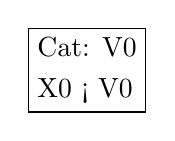
\begin{tikzpicture}[align=left]
%relative placement of nodes starting from the bottom: Future-CP
\node[draw](CPV0){Cat: V0  \\[1mm]
                  X0  <  V0};
\end{tikzpicture}
\zs
Das Zeichen `<' drückt aus, dass X0 unmittelbar vor V0 stehen muss. Goldberg argumentiert
für solche Konstruktionen, da die Kombination aus X0 und V0 nicht der Bedeutung der
Einzelteile entspricht.

Das Futur"=Hilfsverb\is{Verb!Hilfs-} \emph{x{\^a}stan} steht im Persischen immer direkt vor dem
Simplexverb, das in der Vergangenheitsform stehen muss. Goldberg drückt das wie folgt aus:
\eas
Futurhilfsverbkonstruktion nach \citew[\page 127]{Goldberg2003a}:\\
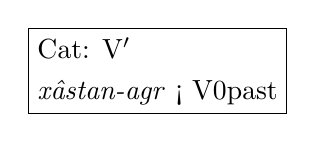
\begin{tikzpicture}[align=left]
\node[draw](Future){Cat: V$'$  \\[1mm]
                    \emph{x{\^a}stan-agr}  <  V0\sub{past}};
\end{tikzpicture}
\zs
Werden komplexe Prädikate ins Futur gesetzt, so steht das Futurhilfsverb zwischen dem X0
und dem V0 des komplexen Prädikats. Goldberg argumentiert, dass das Futurhilfsverb nicht als
Infix behandelt werden sollte, da es Kongruenzmerkmale trägt, die ja zur Flexionsmorphologie
zu zählen sind und da Flexion immer außerhalb von Derivation angewendet wird. Deshalb -- so argumentiert
sie -- liegt ein nicht direkt vorhersagbarer morphologischer Fakt vor, was die Stipulation einer
Futur"=Komplexes"=Prädikat"=Konstruktion rechtfertigt. 
% S. 16
Die Gemeinsamkeiten dieser Konstruktion
mit der Futurkonstruktion und der Komplexes"=Prädikat"=Konstruktion werden durch eine
entsprechende Vererbungshierarchie mit Defaultvererbung erfaßt, die in Abbildung~\vref{goldberg-persisch-vererbung}
dargestellt ist.
\begin{figure}
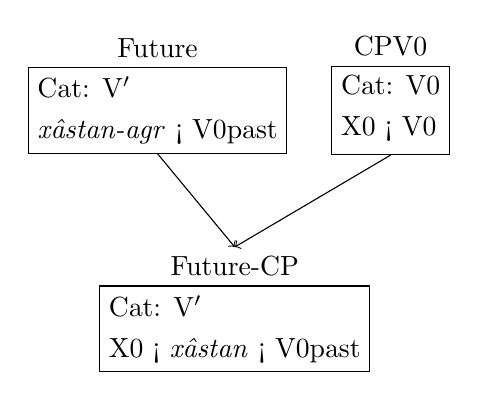
\begin{tikzpicture}[node distance=2.8cm,align=left]
%relative placement of nodes starting from the bottom: Future-CP

% Future-CP
\node[draw](Future-CP) at (0,0){Cat: V$'$  \\[1mm]
                                X0  < \emph{x{\^a}stan} <  V0\sub{past}};
\node[above] (Future-CP label) at (Future-CP.north) {Future-CP};

% Future
\node[draw,xshift=1cm](Future)[above left of=Future-CP label]{Cat: V$'$  \\[1mm]
                                             \emph{x{\^a}stan-agr}  <  V0\sub{past}};
\node[above] at (Future.north) {Future};

% CPV0
\node[draw](CPV0)[above right of=Future-CP label]{Cat: V0  \\[1mm]
                                            X0  <  V0\strut};
\node[above] at (CPV0.north) {CPV0};

\draw[->] (Future.south) to (Future-CP label.north);
\draw[->] (CPV0.south) to (Future-CP label.north);

\end{tikzpicture}
\caption{\label{goldberg-persisch-vererbung}%
Kombination der Komplexes"=Prädikat"=Konstruktion mit der Futurhilfsverbkonstruktion über Mehrfachvererbung mit Defaults}
\end{figure}
Wie man sieht, unterscheiden sich die beiden Konstruktionen, von denen die Futur"=Komplexes"=Prädikat"=Konstruktion
erbt: Sowohl die syntaktische Kategorie (V0 vs.\ V$'$)
als auch die lineare Abfolge der Konstruktionsbestandteile (\emph{x{\^a}stan-agr}  <  V0 vs.\ X0  <  V0)
sind verschieden. Diese Information wird bei der Unterkonstruktion, die von den beiden übergeordneten
Konstruktionen erbt, überschrieben.

\citet[\page 139--140]{Goldberg2003a} % S. 20
argumentiert dagegen, beim Vorliegen nicht"=transparenter Komplexes"=Verb"=Konstruktionen die Bedeutung
einem der Teile zuzuschreiben (also \emph{roSan} oder \emph{kardan} in (\mex{1})),
da die Bedeutung des komplexen Prädikats nur beim Vorliegen beider Bestandteile gegeben ist. 
\ea
\gll roSan kardan\\
     Licht tun\\\nopagebreak
\glt `einschalten'
\z
Das heißt aber, dass es zumindest für diese Fälle Unterkonstruktionen von CPV0 geben muss,
denn CPV0 beschreibt nur den allgemeinen Fall, Idiosynkratisches ist in diesem Muster noch nicht erfaßt.
Um zu erklären, was ein nicht"=transparentes komplexes Prädikat im Futur bedeutet, braucht man aber
eine Konstruktion, die vom nicht"=transparenten komplexen Prädikat und von der Futurkonstruktion erbt,
denn dieser Fall ist in Abbildung~\ref{goldberg-persisch-vererbung} noch nicht erfaßt. Das heißt,
dass es sowohl eine \emph{roSan kardan}"=Konstruktion als auch eine \emph{roSan x{\^a}stan kardan}"=Konstruktion
geben muss. Eine entsprechend modifizierte Hierarchie zeigt Abbildung~\vref{goldberg-persisch-vererbung-korrekt}.
\begin{figure}
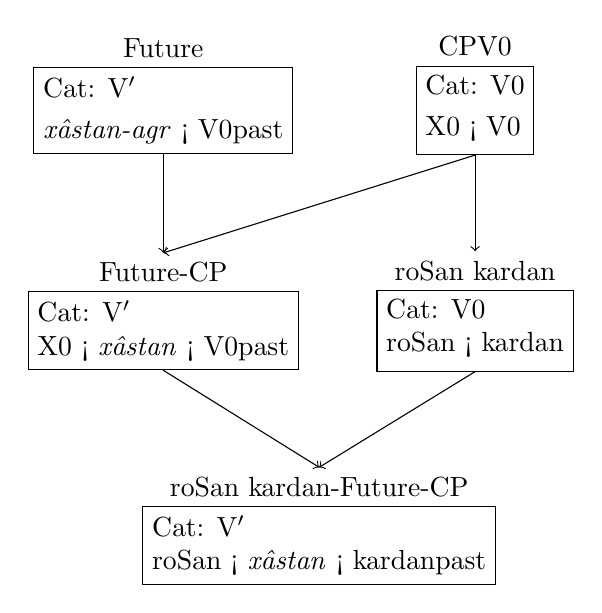
\begin{tikzpicture}[node distance=2.8cm,align=left]
%relative placement of nodes starting from the bottom: x0-xastan-V0
\node[draw](roSan kardan-Future-CP) at (0,0){Cat: V$'$  \\
                                roSan  < \emph{xâstan} <  kardan\sub{past}};
% Label
\node[above] (roSan kardan-Future-CP label) at (roSan kardan-Future-CP.north) {roSan kardan-Future-CP};

\node[draw](Future-CP)[above left of=roSan kardan-Future-CP label]{Cat: V$'$  \\
                                           X0  < \emph{xâstan}  <  V0\sub{past}};

% Label
\node[above] (Future-CP label) at (Future-CP.north) {Future-CP};

\node[draw](roSan kardan)[above right of=roSan kardan-Future-CP label]{Cat: V0  \\
                                            roSan  <  kardan\strut};

% Label
\node[above] (roSan kardan label) at (roSan kardan.north) {roSan kardan};

\node[draw](CPV0)[above of=roSan kardan]{Cat: V0  \\[1mm]
                                           X0  <  V0\strut};

\node[above] at (CPV0.north) {CPV0};

\node[draw](Future)[above of=Future-CP]{Cat: V$'$  \\[1mm]
                                 \emph{x{\^a}stan-agr}  <  V0\sub{past}};

\node[above] at (Future.north) {Future};


\draw[->] (Future-CP.south) to (roSan kardan-Future-CP label.north);
\draw[->] (roSan kardan.south) to (roSan kardan-Future-CP label.north);
\draw[->] (Future) to (Future-CP label);

\draw[->] (CPV0) to (roSan kardan label.north);
\draw[->] (CPV0.south) to (Future-CP label.north);
\end{tikzpicture}
\caption{\label{goldberg-persisch-vererbung-korrekt}%
Modifizierte Hierarchie nach Goldberg}
\end{figure}
Man muss also alle Kombinationen von nicht"=transparenten komplexen Prädikaten mit dem
Futurhilfsverb aufschreiben, was diesen Ansatz sehr unattraktiv macht. Man beachte, dass man sich
hier nicht dadurch aus der Affäre ziehen kann, dass man die Hierarchie, wie das von \citet{Koenig99a}
für Typhierarchien vorgeschlagen wurde, automatisch berechnen läßt, denn Goldbergs Spezifikationen
enthalten Defaults. \citet{Malouf2003a} schlägt zwar solch eine Berechnung auch für Typhierarchien
mit Defaultvererbung vor, schreibt aber, dass auf"|tretende Konflikte nach der Spezifität der 
Werte aufgelöst werden (\emph{while conflicts between default constraints are resolved according
to specificity} S.\,416). Für den Fall in Abbildung~\ref{goldberg-persisch-vererbung} (bzw.\
Abbildung~\ref{goldberg-persisch-vererbung-korrekt}) ist diese Strategie der Default"=Auflösung
nicht anwendbar, denn keine der beiden Beschränkungen \emph{x{\^a}stan-agr}  <  V0\sub{past}
und X0  <  V0 ist spezifischer als die andere. Das heißt, man kann die Berechnung der verschiedenen
Futur-CP"=Konstruktionen für nicht"=transparente komplexe Prädikate keinem automatischen Verfahren überlassen,
sondern muss alle Instanzen per Hand kodieren und die Werte, die die Unterkonstruktion nach Überschreibung
der Default"=Werte haben soll, für jede Konstruktion einzeln spezifizieren. Dass die Abfolge
von X0, Futur"=Hilfsverb und V0 für alle Fälle demselben Muster entspricht, wird in diesem
Ansatz nicht erfaßt, denn die entsprechende Information wird nicht ererbt, sondern für jede
einzelne Konstruktion neu spezifiziert.\footnote{
  Jochen Trommer\aimention{Jochen Trommer} (p.\,M.\ 2006) hat angemerkt, dass man diskontinuierliche
  Konstruktionen annehmen könnte. Die Boxen in Abbildung~\ref{goldberg-persisch-vererbung-korrekt}
  würden dann bedeuten, dass die Konstruktion \emph{x{\^a}stan-agr} und ein V0 dominiert bzw.\ ein X0
  und ein V0. Das `$<$' stünde\is{Linearisierung!-sdom"ane}\is{Linearisierung!-sregel} für Präzedenz
  statt für unmittelbare Präzedenz. Solche Linearisierungsbeschränkungen 
  würden bei der Vererbung keinen Konflikt erzeugen. (Sie könnten sogar unabhängig von den
  Konstruktionen angegeben werden, wie das in GPSG und HPSG gemacht wird.)

  Ähnliche Vorschläge für diskontinuierliche phrasale Konstruktionen wurden von \citet*[\page
  244--248]{Kathol95a} und \citet[Kapitel~4.2]{Crysmann2002a} für Partikelverben im Deutschen gemacht.
  Im Abschnitt~\ref{sec-disc-entry} wurden diese Analysen bereits verworfen.

  Das Problem, dass man Einbettung für die korrekte Erfassung der semantischen Eigenschaften der
  komplexen Prädikate braucht, besteht für Analysen mit diskontinuierlichen Prädikaten genauso wie
  für andere phrasale Analysen.
}

Darüber hinaus ergibt sich ein formales Problem, das auch im Kapitel~\ref{sec-vererbung-koenig} 
über Vererbung im Lexikon schon diskutiert wurde: Die Bedeutung des komplexen Prädikats wird unter
die Bedeutung des Futurhilfsverbs eingebettet. Das läßt sich aber per Vererbung nicht modellieren,
denn der Semantik"=Wert in der Unterkonstruktion überschreibt den Semantik"=Wert der von der
Komplexes"=Prädikat"=Konstruktion kommt \citep[Abschnitt~4.2]{MuellerPersian}. Dieses Problem läßt sich nur lösen, indem man Hilfsmerkmale
verwendet, wie das \citet[\page262]{Kathol94a} und \citet{Koenig99a} gemacht haben (siehe Kapitel~\ref{sec-vererbung-koenig}),
oder indem man verzeigerte Strukturen und Hilfsmerkmale zusammen mit Defaultvererbung verwendet 
\citep{MuellerDefaults}. In jedem Fall werden Hilfsmerkmale gebraucht, was die Theorie im Vergleich
zu Theorien, die ohne solche Merkmale auskommen, abwertet.
\is{Default|)}\il{Persisch|)}\is{Konstruktionsgrammatik (CxG)|)}

Betrachtet man die Daten genauer, stellt man fest, dass ähnliche Datenlagen aus dem Niederländischen
und aus deutschen Dialekten bekannt sind. So kann im Niederländischen\il{Niederländisch}
die Partikel aus Partikelverbkombinationen
durch Hilfsverben vom Verb getrennt werden:
\ea
\gll omdat Carol hem op kon  bellen\footnotemark\\
     weil  Carol ihn an kann rufen\\
\footnotetext{
\citew[\page126]{Koster75a}.
}
\glt `weil Carol ihn anrufen kann'
\z
Genauso muss im Thüringischen\is{Thüringisch} und im Fränkischen\is{Fränkisch} die Partikel vor den
Verben im Verbalkomplex stehen. \citet*[\page356]{Werner94a} gibt die folgenden Beispiele,
die nach Sperschneider\aimention{Heinz Sperschneider} zitiert sind
und im Nordwesten von Sonneberg/""Thüringen gesprochen wurden.
\eal
\label{ex-sonneberg-partikel-phasen}
\ex\iw{anfangen}
\gll a  \ldots{} hot aa   ze schimpfm  gfanga\\
     er {}       hat an   zu schimpfen gefangen\\
\glt `Er hat zu schimpfen angefangen.'
\ex\iw{aufhören}
\gll die  ham  \ldots{}  auf  zu arwettn ghört\\
     die haben {}        auf  zu arbeiten gehört\\
\glt `Die haben zu arbeiten aufgehört.'
\ex
\gll ham   sa  groud  aa mit assn  gfanga\\
     haben sie grade  an mit essen gefangen\\
\glt `Haben sie gerade zu essen angefangen?'
\zl

\noindent
Diese Daten kann man so analysieren, wie das in diesem Kapitel vorgeschlagen
wurde: Die Partikel wird vom Verb selegiert, die Gesamtbedeutung des Partikelverbs ist
beim Partikelverb spezifiziert. Wenn das Verb unter ein Futurhilfsverb eingebettet wird,
wird auch der Bedeutungsbeitrag des Partikelverbs unter die Futursemantik eingebettet.
Für Fälle wie in (\mex{0}) muss man annehmen, dass die Verbpartikel angehoben und
erst nach der Kombination von Hauptverb und Futurhilfsverb abgebunden wird \citep[\page29--30]{Mueller2005c}.


%\section*{Kontrollfragen}

\questions{
\begin{enumerate}
\item Ist \emph{umfahren} ein Partikelverb?
\end{enumerate}
}

%\section*{Übungsaufgaben}

\exercises{
\begin{enumerate}
\item Was braucht man für die Analyse der Sätze in (\mex{1})?
      \eal
      \ex Er kocht die Suppe vor.
      \ex Er arbeitet für Weihnachten vor.
      \zl
      Skizzieren Sie die syntaktischen Aspekte der Einträge für \emph{kochen} und für \emph{vor},
      und falls Sie der Meinung sind, dass keine der Lexikonregeln
      in diesem Kapitel anwendbar ist, geben Sie eine Lexikonregel
      an, die Partikelverben wie \emph{vorarbeiten}, \emph{vorkochen}
      und \emph{vorschlafen} zu ihren Basisverben in Beziehung setzt.

\item Laden Sie die zu diesem Kapitel gehörende Grammatik von der Grammix"=CD
(siehe Übung~\ref{uebung-grammix-kapitel4} auf Seite~\pageref{uebung-grammix-kapitel4}).
Im Fenster, in dem die Grammatik geladen wird, erscheint zum Schluß eine Liste von Beispielen.
Geben Sie diese Beispiele nach dem Prompt ein und wiederholen Sie die in diesem Kapitel besprochenen
Aspekte.

\end{enumerate}
}


\begin{comment}

Zurückgefallen sind das Saarland (von 7 auf 9) und Niedersachsen (von 8 auf 10)
jeweils um zwei Plätze. Jeweils um einen Platz zurück fielen Berlin (von 6 auf 7) und
Rheinland"=Pfalz (von 10 auf 11). c't 6/2005, S.\,102

\end{comment}


\furtherreading{
Partikelverben sind ein Thema, das die Linguisten immer wieder beschäftigt. Unter anderem wird
wieder und wieder diskutiert, ob Partikelverben in der Morphologie oder in der Syntax zu analysieren
sind. Die Anzahl der Publikationen zu Partikelverben im Deutschen und in anderen Sprachen ist
enorm. Hier sei nur auf die Monographie von Barbara \citet{Stiebels96a} und Andrew \citet{McIntyre2001a} und den Sammelband
\citew*{DJMU2002a-ed} verwiesen. Stiebels und McIntyre besprechen bestimmte Klassen von Partikelverben sehr genau.
Im Sammelband werden Partikelverben aus verschiedenen theoretischen Perspektiven beleuchtet.\is{Verb!Partikel-|)}

Die Diskussion der komplexen Prädikate im Persischen ist als \citew{MuellerPersian}
veröffentlicht. Die Diskussion phrasaler Analysen findet man in \citew{MuellerGTBuch1} und in \citew{MWArgSt}.
}

%% -*- coding:utf-8 -*-
%%%%%%%%%%%%%%%%%%%%%%%%%%%%%%%%%%%%%%%%%%%%%%%%%%%%%%%%%
%%   $RCSfile: hpsg-morphologie.tex,v $
%%  $Revision: 1.13 $
%%      $Date: 2008/09/30 09:14:41 $
%%     Author: Stefan Mueller (CL Uni-Bremen)
%%    Purpose: 
%%   Language: LaTeX
%%%%%%%%%%%%%%%%%%%%%%%%%%%%%%%%%%%%%%%%%%%%%%%%%%%%%%%%%



\chapter{Morphologie}
\label{Kapitel-morphologie}
\label{Kapitel-Morphologie}

Die\is{Morphologie|(} Morphologie ist eine eigenständige Teildisziplin der Linguistik mit vielen interessanten
Fragen, die hier nicht einmal gestreift werden können. Im folgenden Kapitel beschränke ich
mich also nur auf einige Grundprobleme. Ich werde die bereits im Kapitel~\ref{sec-lr}
erwähnten Lexikonregeln vorstellen und den alternativen Ansatz, der Affixe als eigenständige
Morpheme annimmt, diskutieren.


\section{Die Phänomene}

In der Morphologie beschäftigt man sich mit Morphen\is{Morph}. Ein \emph{Morph} ist
die kleinste bedeutungstragende Einheit. Haben zwei oder mehr Morphe dieselbe Bedeutung
bei verschiedener Verteilung, spricht man von \emph{Allomorphen}.\is{Allomorph} Eine entsprechende Gruppe
von Allomorphen mit derselben Bedeutung nennt man \emph{Morphem}. 
%% Es gibt freie Morpheme
%% wie \emph{Buch} und \emph{Stuhl}, die ohne

In diesem Kapitel sollen Flexion (Abschnitt~\ref{sec-phen-flexion})
und Derivation (Abschnitt~\ref{sec-phen-derivation}) behandelt werden.

\subsection{Flexion}
\label{sec-phen-flexion}


In\is{Flexion|(} (\mex{1}) liegt eine bestimmte Form der Flexion vor: die Deklination\is{Deklination}.
\eal
\ex Hund\label{bsp-hund-nom}
\ex Hundes\label{bsp-hund-gen}
\ex Hunde
\ex Hunden
\zl
Der Stamm\is{Stamm} \emph{Hund} wird mit bestimmten Endungen (\emph{Suffixen}\is{Suffix})
kombiniert. Welche Endung für den Plural verwendet werden muss, hängt von der Flexionsklasse
des Nomens ab. So kann neben der Endung \suffix{e}, wie sie bei (\mex{0}c) zu beobachten ist, auch
\suffix{en}, \suffix{n}, \suffix{s}, $\varnothing$ den Plural markieren (\emph{Betten},
\emph{Katzen}, \emph{Omas}, \emph{Himmel}). Diese verschiedenen Realisierungsmuster der Pluralendung
faßt man unter dem Begriff Pluralmorphem zusammen. Die verschiedenen Realisierungsformen eines
Morphems\is{Morphem} werden Allomorphe genannt. \suffix{e}, \suffix{en}, \suffix{n}, \suffix{s} und
$\varnothing$ sind also die Allomorphe des Pluralmorphems. $\varnothing$ steht für das Null(allo)morph.
%% Neben Morphemen wie dem Pluralmorphem, das nur gebunden -- also in Kombination mit einem Wortstamm
%% wie \emph{Hund} vorkommen kann -- gibt es auch noch so genannte freie Morpheme. Das sind Morpheme,
%% die nicht mehr mit anderen Morphemen kombiniert werden müssen, sondern gleich so verwendet werden können.

Wie (\mex{1}) zeigt, muss bei einigen Nomina bei der Pluralbildung zusätzlich noch eine Stammumlautung erfolgen:
\eal
\ex Mann\label{bsp-mann-nom}
\ex Mannes\label{bsp-mann-gen}
\ex Männer
\ex Männern
\zl


\noindent
Außer der Flexion der Nomina ist für den in diesem Buch beschriebenen Sprachausschnitt die 
Flexion der Verben (Konjugation\is{Konjugation}) relevant. (\mex{1}) zeigt die finiten Formen für
den Stamm \stem{lach}:
\begin{multicols}{2}
\eal
\label{verb-konjugation-praesens}
\ex Ich lache.
\ex Du  lachst.
\ex Er  lacht.
\ex Wir lachen.
\ex Ihr lacht.
\ex Sie lachen.
\zl
\eal
\label{verb-konjugation-praeteritum}
\ex Ich lachte.
\ex Du  lachtest.
\ex Er  lachte.
\ex Wir lachten.
\ex Ihr lachtet.
\ex Sie lachten.
\zl
\end{multicols}

\noindent
Betrachtet man ein anderes Verb wie \zb \stem{lieb}, stellt man fest, dass die
Endungen gleich sind:
\begin{multicols}{2}
\eal
\ex Ich liebe.
\ex Du  liebst.
\ex Er  liebt.
\ex Wir lieben.
\ex Ihr liebt.
\ex Sie lieben.
\zl
\eal
\ex Ich liebte.
\ex Du  liebtest.
\ex Er  liebte.
\ex Wir liebten.
\ex Ihr liebtet.
\ex Sie liebten.
\zl
\end{multicols}
\noindent
Es liegt also nahe, \zb das Suffix \suffix{st} als Markierung der zweiten Person Singular
anzusehen. Es gibt jedoch auch andere Formen, wie die in (\mex{1}) für das Verb \stem{red}:
\begin{multicols}{2}
\eal
\ex Ich rede.
\ex Du  redest.
\ex Er  redet.
\ex Wir reden.
\ex Ihr redet.
\ex Sie reden.
\zl
\eal
\ex Ich redete.
\ex Du  redetest.
\ex Er  redete.
\ex Wir redeten.
\ex Ihr redetet.
\ex Sie redeten.
\zl
\end{multicols}
\noindent
Im Vergleich zu \stem{lieb} und \stem{lach} steht bei einigen Formen in (\mex{-1})
und (\mex{0}) noch ein zusätzliches \emph{e}. Man könnte jetzt annehmen, dass \stem{red}
einfach ein Verb ist, dass in der zweiten Person Singular die Endung \suffix{est} haben
muss. Es gibt allerdings eine allgemeinere Gesetzmäßigkeit, auf die sich das Auf"|treten
des \emph{e} zurückführen läßt: Das \emph{e} wird eingeführt, wenn an der Morphemgrenze
(der Stelle an der zwei Morpheme zusammenstoßen) ein \emph{d} oder ein \emph{t} auf ein
\emph{s} oder ein \emph{t} treffen. Die entsprechende Regel heißt \emph{e}-Epenthese\is{Epenthese}
und wird wie folgt aufgeschrieben:\footnote{
  Zum Beispiel \citet[\page183]{Eisenberg98a} weist darauf hin, dass diese Regel nicht
  obligatorisch ist, da Formen wie \emph{du botst} und \emph{du rietst} möglich sind.%
}
% du rietst
% du botst
\ea
\label{Regel-e-einfuegung}
+:e $\leftrightarrow$ \{d, t\} \_ \{s, t\}
\z
In (\mex{0}) steht das `+' für die Morphemgrenze. Die Regel besagt, dass die Morphemgrenze
durch ein \emph{e} ersetzt wird, wenn eins der Elemente der Menge \{d, t\} links der Morphemgrenze
steht und eins der Elemente der Menge \{s, t\} rechts der Morphemgrenze.
Eine alternative Schreibweise ist:
\ea
+ $\to$ e / \{d, t\} \_ \{s, t\}
\z
Dies ähnelt den Phrasenstrukturregeln aus Kapitel~\ref{sec-psg}, wobei die Information hinter dem `/'
den Anwendungskontext für die Regel angibt. Verwendet man diese morphophonologischen Regeln,
reicht es anzunehmen, dass \emph{st} die zweite Person Singular markiert. Die Regel erklärt auch,
warum in der dritten Person Singular ein \emph{e} zwischen \stem{red} und \suffix{t} steht,
und es wird plötzlich möglich, die Präteritummarkierung allein dem \infix{t} zuzuordnen 
(\emph{lieb + e} vs.\ \emph{lieb + t + e}): Die Person-\is{Person} und
Numerus"=Markierung\is{Numerus} ist nämlich im Präsens und im Präteritum gleich. Die Formen der zweiten Person unterscheiden sich
lediglich in Bezug auf ein vorhandenes \emph{e}: \emph{lieb+st} vs.\ \emph{lieb+t+e+st}. Dieses
eingefügte \emph{e} wird durch die Regel in (\mex{-1}) erklärt, da das Präteritumsmorphem
auf \emph{t} endet und die Person"=Numerus"=Markierung mit \emph{s} beginnt.\NOTE{liebt+t = liebte erklären}

Neben den bisher diskutierten Fällen gibt es aber noch Verben wie \stem{geb}, die unregelmäßige
Flexionsformen haben:
\begin{multicols}{2}
\eal
\ex Ich gebe.   
\ex Du  gibst.  
\ex Er  gibt.   
\ex Wir geben.  
\ex Ihr gebt.   
\ex Sie geben. 
\zl
\eal
\ex Ich gab.
\ex Du  gabst.
\ex Er  gab.
\ex Wir gaben.
\ex Ihr gabt.
\ex Wir gaben. 
\zl
\end{multicols}
\noindent
Solche Verben werden \emph{starke Verben}\is{Verb!starkes} genannt,
Verben wie \stem{red} werden \emph{schwache Verben}\is{Verb!schwaches} genannt.
Bei den starken Verben wird das Präteritum nicht durch das Einfügen eines \infix{t} gebildet,
sondern durch die Verwendung einer abgelauteten\is{Ablaut} Stammform.
\is{Flexion|)}


\subsection{Derivation}
\label{sec-phen-derivation}

Bei\is{Derivation|(} der Flexion ändert sich die Wortart des flektierten Elements nicht, 
bei der Derivation dagegen ändert sich die Wortart -- und damit
gewöhnlich auch die Bedeutung -- (\mex{1}a,b) bzw.\ (\mex{1}c,d) 
oder die Wortart bleibt gleich (\mex{1}b,c) und die Bedeutung wird geändert.
\eal
\ex \stem{schlag} (Verb)
\ex schlagbar (Adjektiv)
\ex unschlagbar (Adjektiv)
\ex Unschlagbarkeit (Nomen)
\zl
Wie (\mex{1}) zeigt, kann sich bei Derivation auch die Art der Argumente ändern:
\eal
\ex X\sub{akk} auf Y streuen 
\ex Y\sub{akk} mit X bestreuen
\zl
Betrachtet man (\ref{bsp-hund-nom}) und (\ref{bsp-hund-gen}), so ergibt sich bei den beiden
Flexionsformen kein Unterschied in der Bedeutung, es wird lediglich der Kasus des Nomens
markiert. Bei den Pluralformen sieht es schon anders aus: Hier könnte man vermuten,
dass die Pluralflexion gemeinsam mit einer Pluralsemantik auf"|tritt. In Abhängigkeit von
Annahmen, die man in Bezug auf die Syntax der Nominalphrase macht, ist es jedoch
nicht zwingend, die Pluralsemantik den Nomen zuzuordnen. Es könnte auch hier -- wie bei der Kasusmarkierung --
eine rein formale Markierung vorliegen, und die Pluralsemantik würde dann durch den Plural"=Determinator beigesteuert.
Betrachtet man die Konjugationsmuster in (\ref{verb-konjugation-praesens}) und (\ref{verb-konjugation-praeteritum}),
sieht man, dass es hier einen Unterschied in der zeitlichen Lokalisierung des Ereignisses gibt.
Da man diese auch negieren kann, wie (\mex{1}) zeigt, muss sich dieser Zeitbezug auch in der
logischen Repräsentation des Verbs widerspiegeln.\NOTE{FB: Das versteht man nicht ohne weiteres. Was
  hat die Negation damit zu tun?}
\ea
Sie lacht nicht, aber sie wird lachen.
\z

\noindent
Die Linguisten sind sich nicht einig, wie sie Derivation und Flexion genau definieren.
So zählen \citet*[\page263--264]{SWB2003a} die Bildung des Partizips Präsens und Präteritum im Englischen
zur Derivation, weil diese Formen im Französischen noch flektiert werden müssen.
\citet*[\page313]{SWB2003a} behandeln das Passiv\is{Passiv} mittels einer valenzverändernden Lexikonregel.
Alle valenzverändernden Regeln ordnen sie der Derivation zu, weshalb bei ihnen Passivierung
zur Derivation gezählt wird.
\is{Derivation|)}

\section{Die Analyse}

In den beiden folgenden Abschnitten zeige ich, wie Flexion und Derivation mittels lexikalischer Regeln
analysiert werden können. Der Abschnitt~\ref{morph-pv} zeigt, wie die Analyse der Partikelverben, die
im Kapitel~\ref{Kapitel-partikel} vorgestellt wurde, mit der Analyse von Flexion und Derivation zusammenwirkt.

\subsection{Flexion}
\label{sec-morph-flex-anal}
\label{sec-inflection-hpsg}

Im\is{Flexion|(} Kapitel~\ref{Kapitel-Lexikon} haben wir bereits eine Lexikonregel gesehen, die einen Verbstamm zu einer
flektierten Form in Verbindung setzt (S.\,\pageref{passive-lr-mit-phon}). Wie der \phonw aber genau berechnet
wird, wurde bisher nicht erklärt. Betrachtet man die Präsensformen in (\ref{verb-konjugation-praesens}),
so liegt \zb für die zweite Person Singular die folgende Spezifikation
nahe:\is{Kongruenz|(}\NOTE{FB: list-of... muss man erklären}

\eas
\label{lr-verbal-inflection}
Lexikonregel für die zweite Person Singular Präsens (vorläufig):\\
\onems[fin-verb-infl-lr]{
phon   \textit{f\textrm{(\,\ibox{1}, \phonliste{ st })}}\\
synsem$|$loc \onems{ cat   \ibox{2} \onems{ head$|$vform  \type{fin} \\
%                                                        subj  & \eliste \\
                                                  comps  \type{list\_of\_not\_np\_str} $\oplus$ \liste{ NP[\str]$_{2,sg}$ } $\oplus$ \etag\\
                                                } \\
                             cont  \ms[present]{
                                      soa & \ibox{4}\\
%                                       arg2 & \ms[t-overlap]{
%                                              arg1 & \ibox{4}\\
%                                              arg2 & now\\
%                                              }\\
                                      }\\
                       }\\
lex-dtr  \onems[stem]{
           phon   \ibox{1} \\
           synsem$|$loc \ms{ cat  & \ibox{2} \ms{ head  & verb\\
                                                }\\
                             cont & \ibox{4} \\
                         }\\
           }\\
}\is{Lexikonregel!Verbflexion}
\zs
Diese Lexikonregel bildet einen Verbstamm (unter \textsc{lex-dtr}) auf ein Wort ab. Der Typ
\type{fin-verb-infl-lr} ist ein Untertyp von \type{word}. Der \phonw des Ausgabezeichens wird durch
die Funktion \textit{f} berechnet. Der \phonw ist entweder die direkte Verknüpfung des Eingabestamms
mit der Endung \suffix{st} (\emph{lachst}) oder, wenn der Eingabestamm auf \emph{d} oder \emph{t}
endet (siehe Regel (\ref{Regel-e-einfuegung}) auf Seite~\pageref{Regel-e-einfuegung}), die
Verknüpfung des Eingabestamms mit einem -\emph{e}- und dem \suffix{st} (\emph{redest}).  

Eine finite Form kongruiert mit dem Subjekt, wenn es eins gibt. Im Kapitel~\ref{Kapitel-kongruenz}
wurde eine Analyse der Kongruenz vorgestellt, die auf die Index"=Merkmale des Subjekts Bezug nimmt.
In der Lexikonregel in (\mex{0}) wird verlangt, dass das erste Element in der \compsl des Verbs mit
strukturellem Kasus einen Index mit der Person \emph{2} und dem Numerus \emph{sg} haben muss.
Somit ist die Kongruenz zwischen Subjekt und einem Verb wie \emph{lachst} gewährleistet. Die Regel
ist auch so formuliert, dass sie nicht auf das subjektlose Verb \emph{grauen} angewendet werden kann,
denn \emph{grauen} hat kein Argument mit strukturellem Kasus. Die Unterteilung der \compsl in einen
Anfang, der Elemente enthalten kann, die keine Nominalphrasen mit strukturellem Kasus sind, ist
notwendig, um die im Kapitel~\ref{sec-remote-passive-hpsg} diskutierten Beispiele des Fernpassivs\is{Passiv!Fern-} mit
Objektkontrollverben\is{Verb!Objektkontroll-} erfassen zu können.%
\is{Kongruenz|)}

Der \catw des Stammes und der \catw des Wortes sind identisch \iboxb{2}, aber der semantische
Beitrag des Stammes wird unter die Tempus"=Information,\is{Tempus} die vom Suffix beigesteuert wird,
eingebettet.\footnote{ 
  Die Tempus"=Repräsentation ist eine Vereinfachung.%
}

%%\begin{comment}
%% In der Lexikonregel in (\ref{lr-verbal-inflection}) ist nur der Fall für die zweite Person Singular
%% erfaßt. Es stellt sich die Frage, wie die anderen Flexionsformen abgeleitet werden. Eine Möglichkeit besteht
%% darin, parallele Regeln für alle Suffixe zu formulieren. Alternativ kann man die Information aber auch
%% so organisieren, dass alle Flexionsformen (das gesamte Paradigma\is{Paradigma}) am selben Ort spezifiziert
%% sind. Das kann man \zb mit der folgenden Typbeschränkung erreichen:\footnote{
%%   In diesen Repräsentationen ist der Modus\is{Modus} (Indikativ\is{Indikativ}, Konjunktiv\is{Konjunktiv})
%%   der Übersichtlichkeit halber nicht berücksichtigt. In einem vollständigen Flexionsparadigma müssen die entsprechenden Formen
%%   natürlich repräsentiert sein.%
%% }
%% \ea
%% \type{fin-verb-infl-suffix} \impl\\
%% \ms{ phon   & \phonliste{ e }\\
%%                                        tense  & present\\
%%                                        per    & 1\\
%%                                        num    & sg\\
%%                                      } $\vee$
%% \ms{ phon   & \phonliste{ st }\\
%%                                        tense  & present\\
%%                                        per    & 2\\
%%                                        num    & sg\\
%%                                      } $\vee$
%% \ms{ phon   & \phonliste{ t }\\
%%                                        tense  & present\\
%%                                        per    & 3\\
%%                                        num    & sg\\
%%                                      } $\vee$    \ldots
%% \z
%%
%% Die Flexionslexikonregel kann dann wie folgt allgemein formuliert werden:
%% \eas
%% \label{lr-verbal-inflection}
%% Lexikonregel für Verbflexion (vorläufig):\\
%% \ms[fin-verb-infl-lr]{
%% phon   & f\textrm{(\,\ibox{1}, \ibox{2}\,)}\\
%% synsem & \onems{ loc$|$cat   \ms{ head & \ms[verb]{ vform & fin \\
%% %                                                     subj  & \eliste \\
%%                                                        } \\ 
%%                                        comps & \textrm{\ibox{3} (\liste{ NP[\str]$_{\ibox{4},\ibox{5}}$ } $\oplus$ \etag)}\\
%%                                      } \\
%% %%                              cont & \ms[present]{
%% %%                                       soa & \ibox{4}\\
%% %% %                                       arg2 & \ms[t-overlap]{
%% %% %                                              arg1 & \ibox{4}\\
%% %% %                                              arg2 & now\\
%% %% %                                              }\\
%% %%                                       }\\
%%                }\\
%% lex-dtr & \onems[stem]{
%%            phon   \ibox{1} \\
%%            infl \ms[fin-verb-infl-suffix]{
%%                 phon & \ibox{2}\\
%%                 per  & \ibox{4}\\
%%                 num  & \ibox{5}\\
%%                 }\\
%%            synsem$|$loc$|$cat  \ms{ head  & \type{verb}\\
%%                                         comps & \ibox{3}\\
%%                                       }\\
%% %                             cont & \ibox{4} \\
%%            }\\
%% }\is{Lexikonregel!Verbflexion}
%% \zs
%% Durch die Typbeschränkung in (\mex{-1}) ist sichergestellt, dass die Werte der Merkmale unter \textsc{infl}
%% Flexionsaffixen\is{Affix} entsprechen. Der \phonw des Stammes (\ibox{1} in (\mex{0}))
%% wird mit dem \phonw eines Affixes aus der Disjunktion in (\mex{-1}) (\ibox{2} in (\mex{0})) verknüpft.
%% Die entsprechenden Person- und Numerus"=Werte (\iboxt{3} und \iboxt{4}) werden mit den Index"=Werten des Subjekts identifiziert.

%% Die Behandlung der Kongruenz in (\mex{0}) ist jedoch noch nicht für alle bisher diskutierten
%% Fällen verwendbar. Die flektierte Form \emph{graut} kann man mit (\mex{0}) nicht ableiten, da \emph{graut}
%% keine NP mit strukturellem Kasus selegiert. Genauso sind unpersönliche Passive (\mex{1}a) und Anhebungsverben, die Verben
%% ohne Subjekt einbetten (\mex{1}b), nicht analysierbar. Auch der Satz (\ref{bsp-auskosten-fernpassiv-haider}) aus dem Kapitel~\ref{Kapitel-passiv}
%% -- hier als (\mex{1}c) wiederholt -- kann mit der Regel in (\mex{0}) nicht analysiert werden. Das liegt daran, dass
%% die Valenzliste von \emph{wurde} an erster Stelle eine NP mit lexikalischem Dativ enthält (vergleiche Seite~\pageref{abb-remote-pass-da-hm-erlauben}).
%% \eal
%% \ex weil getanzt wurde
%% \ex weil ihm vor der Prüfung zu grauen schien
%% \ex\iw{auskosten}
%% Der Erfolg        wurde uns      nicht auszukosten erlaubt.\footnote{
%%         \citew[\page110]{Haider86c}.%
%% }
%% \label{bsp-auskosten-fernpassiv-haider}
%% \zl
%%
%% Damit die Regel allgemein verwendbar ist, muss man sie wie folgt spezifizieren:
%% \eas
%% \label{lr-verbal-inflection}
%% Lexikonregel für Verbflexion:\\
%% \ms[fin-verb-infl-lr]{
%% phon   & f\textrm{(\,\ibox{1}, \ibox{2}\,)}\\
%% synsem & \onems{ loc \ms{ cat  & \ms{ head & \ms[verb]{ vform & fin \\
%% %                                                     subj  & \eliste \\
%%                                                        } \\ 
%%                                       comps & \ibox{3} \\
%%                                      } \\
%%                           cont & \ms[present]{
%%                                       soa & \ibox{4}\\
%% %                                       arg2 & \ms[t-overlap]{
%% %                                              arg1 & \ibox{4}\\
%% %                                              arg2 & now\\
%% %                                              }\\
%%                                       }\\
%%                       }\\
%%                }\\
%% lex-dtr & \onems[stem]{
%%            phon   \ibox{1} \\
%%            infl \ms[fin-verb-infl-suffix]{
%%                 phon & \ibox{2}\\
%%                 per  & \ibox{4}\\
%%                 num  & \ibox{5}\\
%%                 }\\
%%            synsem$|$loc \ms{ cat  & \ms{ head  & \type{verb}\\
%%                                         comps & \ibox{3}\\
%%                                       }\\
%%                              cont & \ibox{4} \\
%%                            }\\
%%            }\\
%% } $\wedge$ \\
%% subject\_verb\_agreement(\ibox{3},\ibox{4},\ibox{5})\is{Lexikonregel!Verbflexion}
%% \zs
%% Dabei ist subject\_verb\_agreement eine relationale Beschränkung, die erfüllt ist,
%% wenn \ibox{4} = 3 ist \ibox{5} = sg und \ibox{3} keine NP mit strukturellem Kasus enthält
%% oder wenn die erste NP in \ibox{3}, die strukturellen Kasus hat, den \perw \ibox{4} und
%% den \numw \ibox{5} hat.
%% \end{comment}
%% \begin{comment}
%% \subsubsection{Irreguläre Formen}
%%
%% Starke Verben
%%
%% Kopula
%%
%% Lakoff70a
%%
%% corrode, corrosion, corrosive
%% *agress, agression, agressive
%% incite, *incition, *incitive
%%
%% \subsubsection{Fehlende Formen}
%%
%% Im vorigen Abschnitt wurden die unregelmäßigen Formen behandelt. Mitunter kommt es auch vor,
%% dass Formen, die normalerweise zu einem Paradigma gehören, nicht auf"|treten. Beispiele sind
%% Pluraliatanta\is{Pluraliatantum} wie \emph{Leute} und das Futur"=Hilfsverb \emph{werden}, 
%% das nur finit auf"|tritt und auch nicht über Präteritumsformen verfügt.
%%
%% Solche Fälle kann man leicht erfassen, indem man die Information, die Normalerweise im Stamm
%% nicht spezifiziert ist, sondern von den jeweiligen Affixen beigesteuert wird, bereits im Stammeintrag
%% spezifiziert. Dadurch dass man \emph{Leute} mit einem \numw \type{pl} ins Lexikon schreibt, kann
%% kein Singular"=Affix mit dem Nomen kombiniert werden. Nur ein Plural"=Affix wie \zb \suffix{en}
%% ist mit dem Stamm \stem{Leut} kombinierbar, so dass dann die Formen \emph{Leute} und \emph{Leuten}
%% gebildet werden können.
%%
%%\end{comment}
\is{Flexion|)}



%% \ea
%% \ms[derived-stem]{
%% head-dtr & derivational\_affix\\
%% non-head-dtrs & \liste{ stem-or-word }\\
%% }
%% \z

%% \ea
%% \ms[complex-word]{
%% head-dtr & inflectional\_affix\\
%% non-head-dtrs & \liste{ stem }\\
%% }
%% \z

%% \ea
%% \ms[derivation-lexical-rule]{
%% lex-dtr & stem-or-word\\
%% }
%% \z


\subsection{Derivation}
\label{sec-bard}

Die\is{Derivation|(} Behandlung der Derivation soll am Beispiel der \bard erklärt werden. Neben einigen idiosynkratischen
\emph{bar}"=Adjektiven wie \zb \emph{brennbar} gibt es produktiv gebildete \emph{bar}"=Adjektive.
Bei diesen Adjektiven wurde ein Verbstamm eines transitiven Verbs mit dem Suffix \suffix{bar} kombiniert.
\eal
\ex Er löst das Problem.
\ex Das Problem ist lösbar.
\ex Das Problem kann gelöst werden.
\zl
Wie (\mex{0}c) zeigt, ist die \bard äquivalent zu einer Einbettung eines Passivs unter ein Modalverb. Neben
der Modalbedeutung \emph{können} sind auch andere Modalbedeutungen wie \zb \emph{sollen} oder \emph{müssen}
möglich, wie durch Bildungen wie \emph{zahlbar} belegt ist. Für die Bedeutungsrepräsentation der \bard wird
deshalb oft ein allgemeiner Modaloperator\is{Modaloperator} angenommen.

Man sagt, dass ein Muster produktiv\is{Produktivität} ist, wenn es auch auf neu in eine Sprache
aufgenommene Wörter anwendbar ist. So kann man \zb die Wörter \emph{mailbar} und \emph{faxbar}
bilden. Die dazugehörigen Verben \emph{mailen} und \emph{faxen} sind erst im vorigen Jahrhundert in
die deutsche Sprache aufgenommen worden und sind also relativ neue Wörter.

Die produktive Lexikonregel zur Bildung von \emph{bar}"=Adjektiven zeigt (\mex{1}) (siehe auch \citew{Riehemann98a}
zu einer ähnlichen Regel).
\begin{figure}
\eas
\label{lr-bar-adj}
Lexikonregel für die Derivation von Adjektiven mit \bars:\\
\resizebox{\linewidth}{!}{%
\ms[reg-bar-adj-stem]{
phon   & \ibox{1} $\oplus$ \phonliste{ bar }\\
synsem & \onems{ loc  \ms{ cat  & \ms{ head   & \ms[adj]{ 
                                                 subj & \sliste{ \ibox{2} }\\
                                                 }\\
                                        comps & \ibox{3}\\
                                      } \\
                            cont & \ms[modal-op]{
                                    soa & \ibox{4}\\
                                   }\\
                         }\\
               }\\
lex-dtr & \onems[stem]{
           phon   \ibox{1} \\
           synsem$|$loc \ms{ cat  & \ms{ head   & \ms[verb]{
                                                  da & \sliste{ \ibox{5} }\\
                                                  }\\
                                         comps & \sliste{ \ibox{5} NP[\str], \ibox{2} NP[\str] } $\oplus$ \ibox{3}\\
                                       } \\
                             cont & \ibox{4} \\
                          }\\
           }\\
}\is{Lexikonregel!bar-Derivation@\emph{-bar}-Derivation}%
}
\zs
\vspace{-\baselineskip}\end{figure}
Eingabe der Regel ist ein transitives Verb, \dash ein Verb mit zwei Nominalphrasen mit strukturellem Kasus.
Die erste NP -- die auch das designierte Argument sein muss \iboxb{5} -- wird wie bei der Passivierung unterdrückt, 
und die zweite NP \iboxb{2} wird zum Subjekt des durch die Regel lizenzierten Adjektivs.
Der Bedeutungsbeitrag des Verbs \iboxb{4} wird unter einen Modaloperator eingebettet.
\newpage
\noindent
Als Beispiel sei die Lexikonregel auf den Stamm \stem{lös} in (\mex{1})
angewendet. Das Ergebnis der Regelanwendung zeigt (\mex{2}):
\eas
\mbox{\stem{lös}:}\\
\ms{
cat & \ms{ head   & \ms[verb]{
                    da & \sliste{ \ibox{1} }\\
                    }\\
           comps & \liste{ \ibox{1} NP[\str]\ind{2}, NP[\str]\ind{3}} \\
         }\\
cont & \ms[lösen]{ agens & \ibox{2} \\
                   thema & \ibox{3} \\
                 } \\
}
\zs\iw{lösen|uu}

\noindent
\eas
\label{le-fahrbar}
\stem{lösbar}:\\
\ms{
cat & \ms{ head & \ms[adj]{ subj & \sliste{ NP[\type{str}]\ind{3}} \\
                           } \\
           comps & \eliste \\
         }\\
cont & \ms[modal-op]{
       soa & \ms[lösen]{ agens & \etag \\
                    thema & \ibox{3} \\
                  } \\
       }\\
}\iw{fahrbar|uu}
\zs
Die Agens"=Rolle von \emph{lösen} ist nicht an ein Argument des
Adjektivs gelinkt. Das wird durch das leere Kästchen in (\mex{0})
repräsentiert.

Das Ergebnis der Regelanwendung ist ein Adjektivstamm. Dieser muss noch flektiert werden, 
bevor er in der Syntax verwendet werden kann. Je nach Flexion kann das Adjektiv dann
prädikativ oder attributiv gebraucht werden.

Die \bard ist ein Beispiel für die Ableitung eines Stammes aus einem anderen Stamm, aber auch Wörter
können Eingaben für eine Ableitung sein. Ein Beispiel sind die pränominalen Partizipien: In (\mex{1}a) handelt es sich
beim Partizip um ein flektiertes Verb. Die Adjektivbildungsregel, die bereits im Kapitel~\ref{sec-adj-formation}
auf Seite~\pageref{lr-adjective-formation-da-approach} diskutiert wurde, lizenziert einen Adjektivstamm, der dann wieder
flektiert werden muss. In (\mex{1}b) liegt die maskuline Nominativ"=Singular"=Form vor.
\eal
\ex Der Weltmeister wurde geschlagen.
\ex der geschlagene Weltmeister
\zl
\is{Derivation|)}


\subsection{Partikelverben}
\label{morph-pv}

Im folgenden diskutiere ich angebliche Klammerparadoxa, die im Zusammenhang mit der Analyse der
morphologischen Eigenschaften von Partikelverben von vielen Autoren diskutiert wurden. Es handelt sich
dabei um Paradoxa, in denen sowohl morphologische als auch syntaktische und semantische Paradoxa vorzuliegen
scheinen. Würde es sich nur um ein semantisches Paradoxon handeln, so könnte man die von \citet{Egg2004a}
vorgeschlagenen Techniken verwenden, da aber andere Bereiche betroffen sind, ist eine grundlegendere Lösung
des Problems nötig.

Im folgenden sollen drei Fälle betrachtet werden: Der erste Fall stammt aus dem Bereich der
Flexion, die Fälle zwei und drei stammen aus dem Bereich der Derivation.

\citet[\page163]{Bierwisch87a} diskutiert die beiden Analysen für \emph{aufhören}
in Abbildung~\vref{structures-pv}.\footnote{
  Bierwisch nimmt eine morphembasierte Analyse an, ich habe dagegen im vorigen
  Abschnitt eine lexikonregelbasierte Analyse angenommen. Die Analysen sind bis zu einem
  gewissen Grad ineinander übertragbar (siehe Abschnitt~\ref{morphem-vs-lr}).
  Das Bild~\ref{structures-pv}a entspricht der folgenden Struktur:
\vspace{-\baselineskip}
\begin{figure}[H]
\begin{forest}
for tree={font=\footnotesize}
[V
  [P [auf]]
  [V en
    [hör]]]
\end{forest}
%\caption{Struktur mit unärer Regel für Affigierung}
\end{figure}
\vspace{-\baselineskip}
\noindent
Statt einer binären Regel, die ein Affix\is{Affix} mit dem Verbstamm verbindet, wird
im lexikonregelbasierten Ansatz die phonologische Information des Affix innerhalb
der Regel mit der phonologischen Information des Stammes kombiniert.%
}
%
\begin{figure}
a. \begin{forest}
   baseline
   [V
     [P [auf]]
     [V
       [V [hör]]
       [en]]]
\end{forest}
\hspace{2.5cm}b. \begin{forest}
   baseline
   [V
     [V [P [auf]]
        [V [hör]]]
     [en]]
\end{forest}
\caption{Alternative Strukturen für \emph{aufhören}}
\label{structures-pv}
\end{figure}
%
Er argumentiert, dass die Flexionsendung direkt mit dem Stamm verbunden
wird, da sie sensitiv für die Eigenschaften des Stammes ist. Partizipien
wie \emph{aufgehört} machen eine solche Analyse plausibel. Allerdings ist
es so, dass der semantische Beitrag der Flexion sich auf den gesamten Beitrag
des Partikelverbs bezieht und nicht nur auf den Beitrag des Basisverbs.
In \citew{Mueller2002b} habe ich dargelegt, dass diese Beispiele nicht problematisch
sind, da \emph{aufhören} nicht kompositional gebildet ist. Wenn die Partikel
keine Bedeutung beisteuert und die Gesamtbedeutung bereits im Basisverb
enthalten ist, dann entsteht das Problem gar nicht erst. Allerdings gibt
es parallele Fälle mit kompositional gebildeten Partikelverben und für diese
gilt es, das scheinbare Paradoxon aufzulösen. Ich werde im folgenden die
Struktur~\ref{structures-pv}a annehmen und zeigen, dass die im Kapitel~\ref{Kapitel-partikel}
entwickelte Analyse der Partikelverben aufs beste mit der Analyse der
Flexion und Derivation harmoniert.

Für die Struktur~\ref{structures-pv}a sprechen auch die Partizipformen:
\eal
\ex anekeln
\ex angeekelt
\zl
Die Partizipmarkierung \prefix{ge} und \suffix{t} stehen direkt links und rechts
des Verbstammes, die Partikel muss links von \prefix{ge} stehen.
Mit einer Struktur wie der in \ref{structures-pv}b müßte man erklären, wieso
das \emph{ge} zwischen Partikel und Verb steht, da ja bei Annahme dieser
Struktur \emph{aufhör} mit \prefix{ge} und \suffix{t} kombiniert würde.
Auch gibt es eine Regel, die bei der Partizipbildung auf phonologische
Eigenschaften des Verbs Bezug nimmt: Wenn die erste Silbe betont ist,
wird das Partizip mit  \prefix{ge} gebildet (\mex{1}a), ist sie nicht
betont, wird das Präfix \prefix{ge} weggelassen (\mex{1}b).
\eal
\ex ger\'edet, ge\'arbeitet
\ex diskut{\'\i}ert, krak\'eelt
\zl
Für die Anwendung dieser Regel ist es unerheblich, ob das Verb ein
Partikelverb ist oder nicht, einzig die phonologischen Eigenschaften des Verbstamms
sind entscheidend.
\eal
\ex rumgeredet, losgearbeitet
\ex rumdiskutiert, loskrakeelt
\zl
Das wird mit einer Struktur wie der in \ref{structures-pv}a direkt erfaßt.

Das zweite scheinbare Klammerparadoxon ist die \geen.\is{Nominalisierung}
Die \geen ist die einzige diskontinuierliche Nominalderivation im Deutschen.
Sie besteht aus dem Präfix \emph{Ge}- und dem Suffix \suffix{e}. 
Deverbale \emph{Ge}- "~\emph{e}"=Nomina haben die Bedeutung `andauernd/wiederholtes V-en'
und sind mit einer negativen Konnotation verbunden:
\ea
Sein Gepfeife ging ihm auf die Nerven.
\z
Die \geen ist auch bei Partikelverben möglich, und in der Literatur
wurden die beiden Strukturen in Abbildung~\vref{structures-herumgerenne}
vorgeschlagen. 
\begin{figure}
a. \begin{forest}
   baseline
   [N
     [P [herum]]
     [N
       [V [renn]]
       [\gee]]]
\end{forest}
\hspace{2.5cm}b. \begin{forest}
   baseline
   [N
     [V [P [herum]]
        [V [renn]]]
     [\gee]]
\end{forest}
\caption{Alternative Strukturen für \textit{Herumgerenne}}
\label{structures-herumgerenne}
\end{figure}
Die erste Struktur kann ohne weiteres erklären, warum Präfix
und Suffix direkt an den Verbstamm gehen, wohingegen die zweite Struktur
erklären kann, warum das \gee Skopus\is{Skopus} über das gesamte Partikelverb hat.
Die zweite Struktur scheint nötig zu sein, denn \emph{Herumgerenne}
bedeutet  \relation{wiederholt}(\relation{ziellos}(\relation{rennen})) 
und nicht \relation{ziellos}(\relation{wiederholt}(\relation{rennen})).
Siehe zu diesem Punkt \citew[\page106]{Luedeling2001a}. Die letzte Bedeutung
würde man bekommen, wenn man einfach \emph{Gerenne} (\relation{wiederholt}(\relation{rennen}))
mit \emph{herum} (\relation{ziellos}) kombinieren würde.

\noindent
Als drittes Beispiel soll die \bard diskutiert werden: Auch hier scheint
es so zu sein, dass man eigentlich beide Strukturen in Abbildung~\ref{structures-anfahrbar}
braucht: Man möchte, dass das Affix wie bei der \geen direkt mit dem Verbstamm
kombiniert wird, auf der anderen Seite ist aber \bard nur mit transitiven Verben
produktiv, und das Akkusativargument von \emph{anfahren} ist -- wie (\mex{1}) zeigt -- nur durch die
Partikel lizenziert.
\ea
"`Die Kneipen,        Theater  und Geschäfte müssen \emph{anfahrbar} bleiben."'\footnote{
taz, 05.06.1997, S.\,22.% %TAZ-HAMBURG Nr. 5244 Seite 22 vom 05.06.1997
}
\z
\begin{figure}
a. \begin{forest}
   baseline
   [A
     [P [an]]
     [A
       [V [fahr]]
       [bar]]]
\end{forest}
\hspace{2.5cm}b. \begin{forest}
   baseline
   [A
     [V [P [an]]
        [V [fahr]]]
     [bar]]
\end{forest}
\caption{Alternative Strukturen für \emph{anfahrbar}}
\label{structures-anfahrbar}
\end{figure}
Das heißt, dass man sowohl aus Skopusgründen\is{Skopus} als
auch aus Gründen, die mit der Valenz\is{Valenz} von Verben zu tun haben, die
Struktur in Abbildung~\ref{structures-anfahrbar}b zu brauchen scheint.

In der Literatur sind sehr komplexe Verfahren wie \zb Umklammerung\is{Umklammerung} (`rebracketing')
vorgeschlagen worden \parencites[\page165]{Bierwisch87a}[\page934]{SW94a}[\page46]{Stiebels96a}, um mit diesem scheinbaren Paradoxon fertig zu werden. Im folgenden
soll gezeigt werden, dass dies nicht nötig ist und dass man aufbauend auf der
im vorigen Kapitel vorgestellten Analyse der Partikelverben die Flexionsdaten
und Derivationsdaten mit einer Struktur erklären kann, in der die Affixe
jeweils direkt mit dem Verbstamm kombiniert werden. Die Lexikonregel für
die Lizenzierung von Partikelverben hat ja nicht die Partikel eingeführt,
sondern nur eine entsprechende Valenzstelle für die Partikel und eventuell
weitere Argumente bereitgestellt. Die Ausgabe dieser Regel kann dann Eingabe
für die Flexions- bzw.\ Derivationsregeln sein.

Wendet man die Lexikonregel in (\ref{lr-verbal-inflection}) auf das Simplexverb
\stem{lach} in (\ref{le-lachen}) auf S.~\pageref{le-lachen} an, so erhält man 
ein Objekt mit dem \synsemw in (\mex{1}).

\eas
\label{le-lachst}
\mbox{\emph{lachst}:}\\
\ms{
cat & \ms{ head & \ms[verb]{ vform & fin\\
%                             subj  & \eliste \\
                           } \\
           comps & \liste{NP[\type{str}]$_{\ibox{1}~2, sg}$} \\
         }\\
cont & \ms[present]{
        soa & \ms[lachen]{ agens & \ibox{1} \\
                          } \\
        }\\
}\iw{lachen}
\zs

\noindent
Abbildung~\vref{fig-losfaehrst-sem} zeigt, was passiert, wenn man die
Flexionslexikonregel auf die Ausgabe der Partikelverblexikonregel (S.\,\pageref{lr-pv})
anwendet. Diese Abbildung ähnelt der Abbildung~\vref{fig-loslachen-sem}, 
die zur Erklärung der semantischen Kombination von Partikel und Verb benutzt wurde.
Sie enthält zusätzlich jedoch noch Flexionsinformation.
\begin{figure}
\begin{forest}
sm edges
[{V[\cont \ibox{1}]}
   [\ibox{2} Part\feattab{
              \textsc{mod} \ibox{3} [\cont \ibox{4} ]\\
              \cont \ibox{5} \relation{beginnen}\iboxb{4} } [los]]
   [{V[\comps \sliste{ \ldots, \ibox{2} }, \cont \ibox{1} \emph{present}\iboxb{5}]}, l sep+=\baselineskip
%Flexions-LR
      [V\feattab{
          \comps \nliste{ \ldots, \ibox{2} Part[\textsc{mod} \ibox{3}, \cont \ibox{5}] },\\
          \cont  \ibox{5} }, l sep+=\baselineskip,edge label={node[midway,right]{Flexions-LR}}
% PV LR
         [{\ibox{3} V[\cont \ibox{4} \emph{lachen}\iboxb{6}]},edge label={node[midway,right]{PV-LR}}
            [lach]]]]] 
\end{forest}
\caption{Flexion von \stem{lach} und Kombination mit \emph{los}}\label{fig-losfaehrst-sem}
\end{figure}
In der Ausgabe der Partikelverblexikonregel wird der \contw mit dem \contw der Partikel
\iboxb{5} geteilt. Dieser \contw wird in der Ausgabe der Lexikonregel für die Verbflexion
unter die \emph{present}"=Relation eingebettet. Wenn die Partikel mit der
flektierten Form des Stammes \stem{lach} kombiniert wird, wird \ibox{5} innerhalb
der Repräsentation im Verb entsprechend dem von der Partikel beigesteuerten Wert
instantiiert. Im Fall von \emph{los} ist der semantische Beitrag der Partikel
\relation{beginnen}\iboxb{4}, wobei \iboxt{4} der semantische Beitrag des Basisverbs ist.

\begin{comment}
Turning to morphological aspects of inflectional rules,
the participle inflection is dependent on the stress\is{stress} pattern of the verb: If the first
syllable is stressed the participle is formed with \prefix{ge} (\mex{1}a), 
if it is not stressed the \prefix{ge} is omitted (\mex{1}b).
\eal
\ex ger\'edet, ge\'arbeitet
\ex diskut{\'\i}ert, krak\'eelt
\zl
The distribution of \prefix{ge} is the same for simplex and particle verbs. Therefore it is sufficient
to assume that the lexical rule that licenses the participle form is sensitive to the phonological
form of the base verb. The phonological contribution of the particle that will be combined with
the verb is totally irrelevant for the distribution of \prefix{ge}. Since the form of the particle
does not matter as far as the phonology of the participle inflection is concerned, it is unproblematic
that the particle and the base verb are discontinuous in verb-initial sentences.

\citet{Geilfuss-Wolfgang98a} develops an OT\is{Optimality Theory (OT)} 
analysis for the distribution of \prefix{ge}, including the distribution in particle verbs. 
He tries to capture the data on a purely phonological\is{phonology} basis. In order to achieve this, he has to stipulate 
four constraints, one specific to \prefix{ge} and one specific to particle verbs. 
Such stipulations are not necessary in the approach suggested in this book:
\emph{ge-} and \emph{-t} are attached to the stem by an inflectional lexical rule
and the particle is added in a later step as part of the predicate complex.
\end{comment}

Bevor wir uns der derivationellen Morphologie zuwenden, möchte ich die vollständige
Analyse von \emph{loslachst} vorstellen:
Das Ergebnis der Anwendung der Flexionsregel auf den Lexikoneintrag
für das Partikelverb mit dem Stamm \stem{lach}
in (\ref{le-lach-+particle}) auf Seite~\pageref{le-lach-+particle} ist in (\mex{1}) zu sehen:
%\vpageref{le-lachst-+particle}.
%
%\begin{figure}
\newsavebox{\boxxcompvier}
\savebox{\boxxcompvier}{
\onems{ l \onems{ c \onems{ h \onems[particle]{ mod$|$l \onems{
                                                                                            c \ms{ head & verb\\
                                                                                                       comps & \ibox{1}\\
                                                                                                     }\\
                                                                                            cont \ms[lachen]{ agens & \ibox{2} \\
                                                                                                            } \\
                                                                                            }\\
                                                                                   subj \ibox{3} \\
                                                                                 } \\
                                                         comps \ibox{4} \\
                                                       } \\
                                                cont \ibox{5} \\
                                              } \\
                                 }
}
\eas
\label{le-lachst-+particle}
\mbox{\emph{lachst} (Präsens + Selektion einer Partikel):}\\
%\resizebox{\linewidth}{!}{%
\ms{
cat & \onems
\zs
%\vspace{-\baselineskip}\end{figure}

\noindent
Obwohl der Bedeutungsbeitrag der Partikelverbkombination \iboxb{5} noch unterspezifiziert
ist, weil das Verb noch nicht mit der Partikel kombiniert wurde, kann man sich
auf den Beitrag beziehen. Der Beitrag, der von der Partikel kommen wird, wird unter
die \emph{present}"=Relation eingebettet. Wenn die Partikel \emph{los}
mit dem lexikalischen Zeichen in (\mex{0}) kombiniert wird, ergibt sich die Struktur in (\mex{1}).

\eas
\mbox{\emph{los lachst}:}\\
\ms{
cat & \onems{ 
%           head \ms[verb]{ vform & fin\\ } \\           
           comps \liste{NP[\type{str}]$_{\ibox{1}~2, sg}$} \\
         }\\
cont & \ms[present]{
         soa & \ms[beginnen]{ soa & \ms[lachen]{ agens & \ibox{1} \\
                                               }  \\
                           } \\
      }\\
}
\zs
Die Kombination von Partikel und Verb erfolgt so, wie es im Abschnitt~\ref{sec-lr-for-transp-pvs}
beschrieben wurde. Die einzigen Dinge, die hier noch hinzugefügt wurden, sind die
Kongruenzspezifikationen und die semantische Information über Tempus.\is{Tempus}



\subsubsection{Derivationelle Morphologie und Partikelverben}
\label{sec-derivation-hpsg}

In den folgenden Abschnitten zeige ich, dass die \geen und die \bard
mit der bisher eingeführten Analyse der Partikelverben erklärt werden können,
ohne dass irgendwelche Klammerparadoxa entstehen. Die Lexikonregel für die
\bard wurde bereits im Abschnitt~\ref{sec-bard} vorgestellt, die Interaktion mit der
Partikelverbregel wird dann im Abschnitt~\ref{sec-bard-pv} genauer untersucht.
Zuvor möchte ich aber noch die \geen erklären.

\subsubsubsection{Nominalisierungen}

\begin{comment}
As is clear from looking at the examples discussed
in the data section, there are various ways in which
the arguments of a verb can be realized after nominalization has been applied.
The subject or object of the verb can be realized as a \emph{von}"=PP (\mex{1}a), as a postnominal
genitive NP (\mex{1}b), or it may be left implicit (\mex{1}c).
\eal
\ex\iw{Angebrülle}
das Angebrülle von Norbert\footnote{
        taz, 15.10.1993, S.\,16.% %TAZ Nr. 4138 Seite 16 vom 15.10.1993
}
\ex\iw{Rumgeheule}
das Rumgeheule der FDP\footnote{
        taz, 07.01.1998, S.\,3.% %TAZ Nr. 5425 Seite 3 vom 07.01.1998
}
\ex\iw{Herumgerenne}
das Herumgerenne\footnote{
        taz, 01.02.1999, S.\,16.% %TAZ Nr. 5750 Seite 16 vom 01.02.1999
}
\label{ex-herumgerenne-zwei}
\zl
% Accusative objects can also be realized as a \emph{von}"=PP, as a postnominal
% genitive NP, or they may be left implicit.
% \eal
% \ex\iw{Gutfinden}
% \gll das Gutfinden    von Harald Juhnke\\
%      the good.finding of  Harald Juhnke\\
% \glt `Appreciation of Harald Juhnke'
% \ex\iw{Kaputtsanierung}
% \gll die Kaputtsanierung   der Stadt\\
%      the broken.renovation of.the town\\
% \glt `the destructive over-renovation of the town'
% \ex\iw{Kaputtindustrialisierung}
% \gll die Kaputtindustrialisierung\\
%      the broken.industrialization\\
% \glt `the destructive over-industrialization'
% \zl
Rather than giving a detailed account of the various ways in which arguments
can be realized, I will consider the case where all arguments are suppressed.
The main purpose of this subsection is not to provide all the details of argument realizations
in nominal environments, but rather to show how \geens can be accounted
for without any bracketing paradox.
\end{comment}

Die\is{Derivation!Nomen|(}
Lexikonregel in (\mex{2}) lizenziert Nominalisierungen
wie die in (\mex{1}):\footnote{
  In dieser Regel werden die Argumente des Eingabeverbs ignoriert. Natürlich
  gibt es vielfältige Möglichkeiten, diese zu realisieren, was in einem vollständigen
  Ansatz auch berücksichtigt werden muss. Damit die Analyse der Nominalisierung von Partikelverben
  funktioniert, müssen mindestens die komplexbildenden Argumente (die Verbpartikel) der \textsc{lex-dtr} übernommen werden. Dafür werden weiter unten noch Beispiele gegeben.%
}
\ea
das Herumgerenne\footnote{
        taz, 01.02.1999, S.\,16.% %TAZ Nr. 5750 Seite 16 vom 01.02.1999
}
\label{ex-herumgerenne-zwei}
\z

\eas
Lexikonregel für \geenen:\\
\label{lr-gee-nom}%
\ms[ge-e-derived-noun-stem]{
phon & f\textrm{(\,\phonliste{ ge }, \ibox{1}, \phonliste{ e }\,)}\\
synsem & \onems{ loc  \ms{ cat  & \ms{ head   & noun\\
                                       spr & \sliste{ Det }\\
%                                       comps & \eliste\\
                                      } \\
                            cont & \ms{ ind & \ibox{2} \ms{ per & 3\\
                                                            num & sg\\
                                                            gen & neu\\
                                                           }\\
                                         restr & \liste{%
                                                \ms[wiederholtes-ereignis]{
                                                        inst & \ibox{2}\\
                                                        soa & \ibox{3}\\
                                                }}\\   
                                      }\\                                 
                         }\\
               }\\
lex-dtr & \onems[stem]{
           phon   \ibox{1} \\
           synsem$|$loc \onems{ cat$|$head \type{verb}\\
                                cont    \ibox{3} \\
                        }\\
           }\\
}\is{Lexikonregel!ge- -e Nominalisierung@\emph{Ge- -e}-Nominalisierung}
\zs

\noindent
$f$ ist dabei wieder eine Funktion, die den \phonw des Eingabezeichens
mit \gee kombiniert. 
Das \suffix{e} ist optional, wenn das Eingabenomen -- wie \zb in \emph{Rumgeballer} --
mit einer unbetonten\is{Betonung} Silbe \suff{er}, \suff{el}, \suff{en} endet.
% Gallmann phonologisch gesteuert =/= phonologisch bedingt
Das Ergebnis der Regelanwendung ist ein nominaler Stamm. Dieser Stamm
muss flektiert werden, damit er in der Syntax benutzt werden kann.\footnote{
        Siehe auch \citet[\page118]{Koenig99a} für einen
        ähnlichen Vorschlag zur Interaktion von Flexion und Derivation.%
}
Nullflexion\is{Flexion!Null-} führt zu einer Form\is{Kasus!morphologischer}
im Nominativ, Dativ bzw.\ Akkusativ. Wird bei der Flexion ein \suffix{s} angehängt,
bekommt man die Genitiv"=Form.

\begin{comment}
% Olsen stellt Gemeinsamkeiten zwischen lexikalisierten Ge-Nomina (Geklimper) und motivierten
% Versionen (Geklimper) her. Diese kann man durch Typen modellieren.

The rule applies to all verbs. The valence properties of the nominalized verb
are ignored since this lexical rule licenses only the bare noun with a determiner
without any complements that could be inherited from the verb. Following 
\citet[Chapter~1]{ps2} and \citet{Demske2001a}, I assume that the noun selects a determiner,
\ie, I assume an NP analysis rather than a DP\is{determiner phrase}
analysis, but the rule in (\mex{0}) could be easily changed. For a DP
analysis in HPSG see \citew{Abb94}. A special variant of a DP analysis
can be found in \citew{Netter94} and \citew{Netter98-Eng}.
\end{comment}

Da die Nomina, die mittels \geen abgeleitet sind, Neutra sind, lizenziert
die Lexikonregel ein Nomen mit einem referentiellen Index mit dem Genus"=Wert \type{neu}.
\geenen haben keine Pluralformen\is{Plural} \citep[\page34]{Bierwisch89a}, was dadurch
erfaßt wird, dass der Numerus"=Wert\is{Numerus} in der Ausgabe der Lexikonregel ebenfalls
spezifiziert ist. Pluralaffixe können deshalb nicht mit durch die Lexikonregel
in  \pref{lr-gee-nom} lizenzierten Stämmen kombiniert werden. 
Der referentielle Index \iboxb{2} ist identisch mit dem Wert des \textsc{inst}"=Merkmals
der \relation{wiederholtes-ereignis}"=Relation.


% das Grauen vor dem Henker -> auch subjektlose Verben koennen nominalisiert werden

Als Beispiel für die Anwendung der Regel soll zuerst die Ableitung von \emph{Gerenne} diskutiert
werden. Als Eingabe zur Lexikonregel dient der Stamm des Simplexverbs \stem{renn}.
Der \locw für \stem{renn}, der in (\mex{1}) angegeben ist, ist parallel
zu dem bereits diskutierten für \stem{lach}.

\eas
\stem{renn}:\\
\ms{
cat & \ms{ head & verb \\
           comps & \liste{NP[\str]\ind{1}} \\
         }\\
cont & \ms[rennen]{ agens & \ibox{1} \\
                  } \\
}\iw{rennen|uu}
\zs

\noindent
Das Ergebnis der Anwendung der Lexikonregel in (\ref{lr-gee-nom}) auf (\mex{0})
ist (\mex{1}).

\eas
\label{le-gerenne}
\stem{Gerenne}:\\
%\resizebox{\linewidth}{!}{%
\ms{ cat  & \ms{ head   & noun\\
                              spr & \sliste{ Det }\\
                              comps & \eliste\\
                            } \\
                  cont & \ms{ ind & \ibox{2} \ms{ per & 3\\
                                                  num & sg\\
                                                  gen & neu\\
                                                }\\
                              restr & \liste{ 
                                      \ms[wiederholtes-ereignis]{
                                                        inst & \ibox{2}\\
                                                        soa & \ms[rennen]{ agens & \etag \\
                                                                        } \\
                                                        }}\\   
                            }\\ 
}
%}
\zs

\noindent
Die Agens"=Rolle von \emph{rennen} ist nicht an ein Element in der Valenzrepräsentation
des Nomens gelinkt, weshalb der Wert des \textsc{agens}"=Merkmals in (\mex{0}) 
als leeres Kästchen visualisiert ist.
% Jacobs94a -> definitheitsneutrale Variablen
% The nominalization
% rule has to take care of the existential quantification of this argument.

Als nächstes soll die Analyse des Wortes \emph{Herumgerenne} vorgeführt werden.
Wie \emph{los} kann die Partikel \word{herum} in der relevanten Lesart nur mit intransitiven Verben kombiniert werden.
Das zeigt (\mex{1}):
\eal
\ex[]{\iw{herumrennen}\iw{herumhüpfen}
Karl rennt / hüpft herum.
}
\ex[]{\iw{herumlesen}
Karl liest (in dem Buch) herum.
}
\ex[*]{
Karl liest das Buch herum.
}
\zl
Es gibt viele Bedeutungen von \emph{herum}. Die Bedeutung,
die hier von Interesse ist, fügt der Bedeutung des Basisverbs
eine Komponente hinzu, in der enthalten ist, dass die Aktion
des Basisverbs ziellos ist.
(\mex{1}) zeigt den \locw des Lexikoneintrags von \emph{herum}.
Der \locw ist parallel zu dem von \emph{los}, der auf Seite~\pageref{le-los-asp}
angegeben wurde.
%
\eas
\label{le-herum-part}
\mbox{\emph{herum}:}\\
\ms{
cat & \ms{ head & \ms[particle]{ mod  & \textrm{V[\textsc{comps} \sliste{ NP[\str] }, \textsc{cont} \ibox{1}]} \\
                                subj & \eliste \\
                              } \\
           comps & \eliste \\
         }\\
cont & \ms[ziellos]{ soa & \ibox{1} \\
                   } \\
}
\zs

%
\noindent
Die Analyse von \emph{Herumgerenne} zeigt Abbildung~\vref{fig-herumgerenne}.
\begin{figure}
\begin{forest}
sm edges
[{N[\cont \ibox{1}]}
  [\ibox{2} Part\feattab{
              \textsc{mod} \ibox{3} [\cont \ibox{4} ]\\
              \cont \ibox{5} \relation{ziellos}\iboxb{4} } [herum]]
  [{N[\comps \sliste{ \ldots, \ibox{2} }, \cont \ibox{1} \ldots{}
    \relation{wiederholtes-ereignis}\iboxb{5}]}, l sep+=\baselineskip
%& \hspace{27ex}\gee-Nominalisierungs-LR\\[4ex]
    [V\feattab{
       \comps \nliste{ \ldots, \ibox{2} Part[\textsc{mod} \ibox{3}, \cont \ibox{5}] },\\
       \cont  \ibox{5} }, l sep+=\baselineskip, edge label={node[midway,right]{\gee-Nominalisierungs-LR}}
%&\hspace{8ex}PV LR\\[4ex]
     [{\ibox{3} V[\cont \ibox{4} \relation{rennen}\iboxb{6}]}, edge label={node[midway,right]{PV-LR}}
       [renn]]]]]
\end{forest}
\caption{Analyse von \emph{Herumgerenne}}\label{fig-herumgerenne}
\end{figure}
%
Um \emph{Herumgerenne} abzuleiten, muss zuerst die Lexikonregel für produktive Partikelverbbildungen
((\ref{lr-pv}) auf Seite~\pageref{lr-pv}) auf den im Lexikon gelisteten Eintrag \stem{renn} angewendet
werden. Das Ergebnis der Regelanwendung ist ein lexikalisches Zeichen,
das eine Partikel selegiert \iboxb{2}.
Der Bedeutungsbeitrag dieser Partikel \iboxb{5} wird mit der Bedeutung
des lexikalischen Zeichens identifiziert, das durch die Partikelverblexikonregel
lizenziert wird. Die Nominalisierungsregel wird auf dieses Zeichen angewendet
und bettet dessen semantischen Beitrag unter die Relation \relation{wiederholtes-ereignis} ein.
Im nächsten Schritt wird das Nomen flektiert (in Abbildung~\ref{fig-herumgerenne} nicht dargestellt)
und danach mit der Partikel kombiniert. Da das Nomen 
der Kopf in einer head"=cluster"=Struktur ist, ist sein Bedeutungsbeitrag \iboxb{1} 
identisch mit dem Beitrag der Mutter in der Struktur. Die Bedeutung der Partikel
ist bei der Kombination dann bekannt (sowohl die Bildung von \emph{Losgerenne}
als auch die von \emph{Herumgerenne} wäre mit dem \emph{gerenne}, das eine Partikel
selegiert, möglich). Über ihren \modw kann die Partikel auf den semantischen
Beitrag des Verbs zugreifen \iboxb{4} und diesen unter die \relation{ziellos}"=Relation
einbetten. Das Ergebnis ist \relation{ziellos}(\relation{rennen}\iboxb{6}). 
Da der semantische Beitrag durch die Nominalisierungsregel unter \relation{wiederholtes-ereignis}
eingebettet wird, ist die semantische Repräsentation für die gesamte Nominalisierung
\relation{wiederholtes-ereignis}(\relation{ziellos}(\relation{rennen}\iboxb{6})), was genau dem
erwünschten Resultat entspricht.

Nach dieser Skizze der Analyse sollen jetzt die genauen Merkmalbeschreibungen angegeben werden:
(\mex{1}) zeigt die Merkmalbeschreibung des Lexikoneintrags, der durch die Partikelverblexikonregel
in \pref{lr-pv} auf Seite~\pageref{lr-pv} lizenziert wird. Dieser Eintrag ähnelt dem von \stem{lach}, 
der in (\ref{le-lach-+particle}) gezeigt wurde. Der einzige Unterschied besteht
in dem Teil der semantischen Repräsentation, der sich unterscheidet,
da er vom Basisverb (\stem{lach} vs.\ \stem{renn}) kommt.

\newsavebox{\boxxcompfuenf}
\savebox{\boxxcompfuenf}{
\onems{ l \onems{ c \onems{ h \onems[particle]{ mod$|$l \onems{
                                                                                            cat \ms{ head & verb\\
                                                                                                   comps & \ibox{1} \\
                                                                                                 }\\
                                                                                            cont \ms[rennen]{ agens & \ibox{2} \\
                                                                                                            } \\
                                                                                            }\\
                                                                                   subj \ibox{3} \\
                                                                                 } \\
                                                         comps \ibox{4} \\
                                                       } \\
                                                cont \ibox{5} \\
                                              } \\
                                 }
}
\eas
\label{le-renn-+particle}
\mbox{\emph{renn-} (mit Selektion einer Partikel):}\\
%\resizebox{\linewidth}{!}{%
%\scalebox{0.9}{%
\onems{
cat \ms{ %head & verb \\
       comps & \begin{tabular}[t]{@{}l@{}}
                \textrm{(}\,\ibox{1} \liste{NP[\str]\ind{2}} \textrm{)} $\oplus$ \ibox{3} $\oplus$ \ibox{4} $\oplus$ \\[3mm]
                \liste{\usebox{\boxxcompfuenf} } \\
                \end{tabular}
     }\\
cont \ibox{5} \\
}
%}
\zs
%

\noindent
Die Lexikonregel für \geen wird auf diesen Eintrag angewendet.
Das Ergebnis zeigt (\mex{1}).
\newsavebox{\boxxcompsechs}
\savebox{\boxxcompsechs}{
\onems{ l \onems{ c \onems{ h \onems[particle]{ mod$|$l \onems{
                                                                                            c \ms{ head & verb \\
                                                                                                   comps & \liste{NP[\str]\ind{1}} \\[1mm]
                                                                                                 }\\
                                                                                            cont \ms[rennen]{ agens & \ibox{1} \\
                                                                                                            } \\
                                                                                            }\\
%                                                                                   subj \ibox{2} \\
                                                                                 } \\
%                                                         comps \ibox{3} \\
                                                       } \\
                                                cont \ibox{2} \\
                                              } \\
                                 }
}
\eas
\label{le-gerenne+particle}
\mbox{\emph{gerenne-} (mit Selektion einer Partikel):}\\
\onems{
cat \onems{ head \type{noun} \\
            spr \sliste{ Det }\\
           comps \sliste{ \usebox{\boxxcompsechs}} \\
         }\\
cont \ms{ ind & \ibox{3} \ms{ per & 3\\
                                                            num & sg\\
                                                            gen & neu\\
                                                           }\\
                                         restr & \liste{ 
                                                \ms[wiederholtes-ereignis]{
                                                        inst & \ibox{3}\\
                                                        soa & \ibox{2}\\
                                                }}\\   
                                      }\\       
}
\zs

\noindent
Dieser Stamm wird durch eine Flexionsregel flektiert. Das Ergebnis 
für Nominativ, Dativ und Akkusativ unterscheidet
sich von (\mex{0}) nur durch die Instantiierung der Kasuswerte, weshalb
die entsprechende Merkmalbeschreibung hier nicht gesondert aufgeführt wird.
In der folgenden Struktur werden die Kasusinformation und auch die Strukturteilungen,
die für die Kongruenz mit dem Determinator benötigt werden, der Übersichtlichkeit
halber weggelassen.

Die Bedeutung von \emph{rennen} + Partikel \iboxb{2} ist ein Argument der
Relation \relation{wiederholtes-ereignis}. In
(\mex{0}) ist der Wert von \iboxt{2} noch unterspezifiziert,
aber wenn (\mex{0}) mit einer Partikel kombiniert wird, wird \iboxt{2}
instantiiert. Das Ergebnis der Kombination der Partikel \emph{herum} in \pref{le-herum-part}
mit (\ref{le-gerenne+particle}) zeigt (\mex{1}).

\eas
\label{fs-Herumgerenne}
\emph{Herumgerenne}:\\
%\resizebox{\linewidth}{!}{%
\ms{
cat & \ms{ head & noun \\
           spr & \sliste{ Det } \\
           comps & \eliste\\
         }\\
cont & \ms{ ind & \ibox{2} \ms{ per & 3\\
                                                            num & sg\\
                                                            gen & neu\\
                                                           }\\
                                         restr & \liste{ 
                                                \ms[wiederholtes-ereignis]{
                                                        inst & \ibox{2}\\
                                                        soa & \ms[ziellos]{ soa & \ms[rennen]{ agens & \etag \\
                                                                                                    } \\ 
                                                              }\\
                                                }}\\   
                                      }\\        
}
%}
\zs

\noindent
Wie beim einfachen \emph{Gerenne} in (\ref{le-gerenne}) ist das
Agens von \emph{rennen} in (\mex{0}) nicht spezifiziert. 
% The nominalization rule takes care of the 
% existential quantification of this argument. 
Die Skopusbeziehungen zwischen Partikel und dem semantischen Material,
das von der Derivation beigesteuert wird, ist korrekt, Mechanismen
wie Umklammerung werden nicht gebraucht, da in dieser Analyse kein
Klammerparadoxon vorliegt.

\begin{comment}
The derivation with object predicatives and resultatives is completely analogous:
The rule in (\ref{lr-gee-nom}) is applied to the lexical entry for the object predicative
\emph{find}- (`find') producing \stem{gefinde}, which is then combined with 
\emph{schön} (`beautiful') to yield \emph{Schöngefinde}\iw{Schöngefinde} (`beautiful.finding').
In the case of resultative constructions, the listed entry for \emph{schlag}- (`to hit')
is fed into the lexical rule (\ref{lr-result}) for resultative constructions.
The output of this rule is the input to (\ref{lr-gee-nom}), yielding
\stem{geschlage}, which is then combined with \emph{tot} (`dead'),
resulting in \word{Totgeschlage} (`dead.beating').
\end{comment}
\is{Derivation!Nomen|)}

Nach der Behandlung von Flexion und \geen wende ich mich nun
dem schwierigsten Fall zu: der \bard.

\subsubsubsection{Adjektivderivation}
\label{sec-bard-pv}

Die\iw{\bars|(}%
\is{Derivation!Adjektiv|(}
Interaktion der \bard mit Partikelverben ist die
komplexeste, da sowohl Beschränkungen in Bezug auf Valenz\is{Valenz}
als auch Skopusbeziehungen\is{Skopus} eine Rolle spielen.
Auf Seite~\pageref{lr-bar-adj} haben wir bereits die
Lexikonregel \pref{lr-bar-adj} für \bard vorgestellt.

Im folgenden sollen komplexe Derivationen wie \emph{anfahrbar}
in (\mex{1}) diskutiert werden:
\ea
 "`Die Kneipen,        Theater  und Geschäfte müssen \emph{anfahrbar} bleiben."'\footnote{
taz, hamburg, 05.06.1997, S.\,22.% %TAZ-HAMBURG Nr. 5244 Seite 22 vom 05.06.1997
}
\z
\emph{anfahren} ist nach einem produktiven Muster gebildet, und die entsprechende
Partikelverbregel wurde bereits im Kapitel~\ref{sec-lr-for-transp-pvs} besprochen.
Die Diskussion der Interaktion der Partikelverbregel mit der \bard wird in zwei Teile geteilt: Zuerst
diskutiere ich die Beschränkungen in Bezug auf die Verbvalenz, und dann zeige ich,
dass die bisher formulierten Regeln die Bedeutung von \barden mit Partikelverben adäquat
erfassen.

Abbildung~\vref{fig-p-fahrbar-pv-lr} zeigt die Anwendung der Partikelverbregel.
\begin{figure}
\begin{forest}
sm edges
[{V[\comps \ibox{1} $\oplus$ \ibox{2} $\oplus$ \ibox{3} $\oplus$ \nliste{ Part[\subj \ibox{2}, \comps \ibox{3}] }]}, l sep+=\baselineskip
  [{V[\comps \ibox{1} \sliste{ NP[\str] }]}, edge label={node[midway,right]{PV-LR}} 
    [fahr]]]
\end{forest}
\caption{Anwendung der Partikelverbregel auf \stem{fahr}}\label{fig-p-fahrbar-pv-lr}
\end{figure}
Das Ergebnis der Anwendung ist ein Lexikoneintrag mit einem unterspezifizierten
\compsw. Der letztendliche Wert wird durch die Partikel bestimmt, sobald die Partikel
mit dem Kopf"=Verb kombiniert wird.

Die Lexikonregel für die \bard verlangt als Eingabe ein Verb mit einem Objekt mit strukturellem
Kasus. Da die Ausgabe der Partikelverbregel kompatibel mit dieser Anforderung ist, kann
die Lexikonregel für die \bard auf das Partikelverb angewendet werden. Das wird in Abbildung~\vref{fig-p-fahrbar-val}
gezeigt.
\begin{figure}
\begin{forest}
sm edges
[{Adj[\subj \sliste{ \ibox{4} }, \comps \ibox{5} $\oplus$ \nliste{ Part[\subj \ibox{2}, \comps \ibox{3}] }]}, l sep+=\baselineskip
%\hspace{19ex}\bard LR\\[4ex]
  [{V[\begin{tabular}[t]{@{}l@{}}
      \comps \ibox{1} $\oplus$ \ibox{2} $\oplus$ \ibox{3} $\oplus$ \nliste{ Part[\subj \ibox{2},
        \comps \ibox{3}] }]\\
                $\wedge$ \ibox{1} $\oplus$ \ibox{2} $\oplus$ \ibox{3} = \sliste{ NP[\str], \ibox{4}
                  NP[\str] } $\oplus$ \ibox{5} 
      \end{tabular}}, l sep+=\baselineskip, edge label={node[midway,right]{\bard-LR}}
%
%\hspace{8ex}PV LR\\[4ex]
     [{V[\comps \ibox{1} \sliste{ NP[\str] }]}, edge label={node[midway,right]{PV-LR}}
        [fahr]]]]
\end{forest}
\caption{Anwendung der Lexikonregel für die \bard auf \stem{fahr} mit selegierter Partikel}\label{fig-p-fahrbar-val}
\end{figure}
Der \compsw des Eingabezeichens muss eine Liste sein, die mit zwei Nominalphrasen mit strukturellem Kasus
beginnt (\sliste{ NP[\str], \ibox{4} NP[\str] } $\oplus$ \ibox{5}\,).
Da der \compsw des Eingabezeichens für die \bard in Abbildung~\ref{fig-p-fahrbar-val} die
Verknüpfung der \compsl des Basisverbs mit dem \subjw und dem \compsw der selegierten Partikel ist, können nur Partikeln, die eine
NP[\str] in ihrer \subjl oder in ihrer \compsl haben, mit dem Ergebnis der \bard kombiniert werden.

Abbildung~\vref{fig-anfahrbar-val} zeigt die Kombination von \emph{an}$_5$ und \emph{fahrbar}.\footnote{
  Zu den verschiedenen Formen der Partikel \emph{an} siehe Seite~\pageref{verschiedene-ans}.%
}
\begin{figure}
\begin{forest}
sm edges
[{Adj[\subj \sliste{ \ibox{4} }, \comps \ibox{5} \eliste]}
   [\ibox{6} Part\feattab{
                 \subj \ibox{2} \sliste{ NP[\str] },\\
                 \comps \ibox{3} \eliste } [an]]
   [{Adj[\subj \sliste{ \ibox{4} }, \comps \ibox{5} $\oplus$ \sliste{ \ibox{6} }]}, l sep+=\baselineskip
%& \hspace{19ex}\bard LR\\[4ex]
      [{V[\begin{tabular}[t]{@{}l@{}}
                \comps \ibox{1} $\oplus$ \ibox{2} $\oplus$ \ibox{3} $\oplus$
                \nliste{ Part[\subj \ibox{2}, \comps \ibox{3}] }]\\
                $\wedge$ \ibox{1} $\oplus$ \ibox{2} $\oplus$ \ibox{3} = \sliste{ NP[\str], \ibox{4} NP[\str] } $\oplus$ \ibox{5}\\
               \end{tabular}}, l sep+=\baselineskip, edge label={node[midway,right]{\bard-LR}}
%&\hspace{8ex}PV LR\\[4ex]
         [{V[\comps \ibox{1} \sliste{ NP[\str] }]}, edge label={node[midway,right]{PV-LR}}
           [fahr]]]]] 
\end{forest}
\caption{Kombination von \emph{an}$_5$ und \emph{fahrbar} (Valenz)}\label{fig-anfahrbar-val}
\end{figure}
Die Partikel hat eine NP[\str] in ihrer \subjl \iboxb{2}. Der \compsw der Partikel \iboxb{3} ist die leere Liste.
Die Verknüpfung von \ibox{2} and \ibox{3} ist deshalb eine Liste, die genau eine NP[\str] enthält. 
Dieses Element wird mit dem Element \iboxt{4} identifiziert, das von der Lexikonregel für die \bard zum Subjekt angehoben
wird. Deshalb hat das Adjektiv \emph{anfahrbar} als Subjekt das Element, das durch die Partikel eingeführt
wurde, und die \compsl von \emph{anfahrbar} ist leer. Weil es außer den beiden NPen kein anderes
Element in der Verknüpfung von \ibox{2} and \ibox{3} gibt, ist \iboxt{5} die leere Liste.

Interessanterweise ermöglichen die Regeln nicht nur die Analyse von \emph{anfahrbar}, sondern
schließen auch ungrammatische Beispiele wie das in (\mex{1}b) aus.\footnote{
  Das Wort \emph{losfahrbaren} ist vorstellbar in Wortgruppen wie \emph{die losfahrbaren Autos}.
  In dieser Verwendung liegt aber nicht die Partikel \emph{los} vor, die bisher diskutiert
  wurde, sondern ein \emph{los} mit der Bedeutung \emph{ab} oder \emph{lose}. Die \bard
  nimmt dann als Eingabe einen Verbstamm, wie er in
  Resultativkonstruktionen\is{Resultativkonstruktion} verwendet werden 
  kann. Siehe hierzu \citew[\page380--381]{Mueller2002b}.%
}
\eal
\ex[]{\iw{anfahrbar|)}
die anfahrbaren Geschäfte
}
\ex[*]{
die losfahrbaren Geschäfte
}
\zl
Der Grund hierfür ist, dass \emph{los} keine Argumente einführt. Da \emph{los} nur mit intransitiven
Verben kombiniert werden kann, ist das Ergebnis einer solchen Kombination wieder ein intransitives Verb.
Obwohl es eine Form \emph{fahrbare} gibt, die eine Partikel selegiert, kann diese nicht mit \emph{los}
kombiniert werden, da die Beschränkung, die durch die Lexikonregel für die \bard eingeführt wurde
(\,\ibox{1} $\oplus$ \ibox{2} $\oplus$ \ibox{3} = \sliste{ NP[\str], \ibox{4} NP[\str] } $\oplus$ \ibox{5}\,) 
verletzt wäre: \ibox{1} $\oplus$ \iboxt{2} $\oplus$ \iboxt{3} würde nur ein Element enthalten,
nämlich das Subjekt von \stem{fahr}.

Wenden wir uns nun der Bedeutungsrepräsentation in der Analyse von \emph{anfahrbar} zu,
die in Abbildung~\vref{fig-anfahrbar-sem} gezeigt wird.
\begin{figure}
\begin{forest}
sm edges
[{Adj[\cont \ibox{1}]}
   [\ibox{2} Part\feattab{
                 \textsc{mod} \ibox{3} [\cont \ibox{4} ]\\
                 \cont \ibox{5} \relation{gerichtet-auf}(\,\ibox{4}, \ibox{6}\,) } [an]]
   [{Adj[\comps \sliste{ \ibox{2} }, \cont \ibox{1} \emph{modal-op}(\,\ibox{5}\,)]}, l sep+=\baselineskip
%& \hspace{19ex}\bard LR\\[4ex]
      [V\feattab{
        \comps \nliste{ \ldots, \ibox{2} Part[\textsc{mod} \ibox{3}, \cont \ibox{5}] },\\
        \cont  \ibox{5} }, l sep+=\baselineskip, edge label={node[midway,right]{\bard-LR}}
%&\hspace{8ex}PV LR\\[4ex]
          [{\ibox{3} V[\cont \ibox{4} \emph{fahren}\iboxb{7}]}, edge label={node[midway,right]{PV-LR}}
            [fahr]]]]]
\end{forest}
\caption{Kombination von \emph{an}$_5$ und \emph{fahrbar} (Semantik)}\label{fig-anfahrbar-sem}
\end{figure}
Die Partikelverblexikonregel führt eine Partikel in die \compsl ein,
die die Eingaberepräsentation über \textsc{mod} selegiert \iboxb{3}. In der Ausgabe der
Lexikonregel wird der \contw \iboxb{5} mit dem \contw der Partikel in der \compsl identifiziert.
Die Lexikonregel für die  \bard bettet diesen \contw unter einen Modaloperator \emph{modal-op} ein.
Zu diesem Zeitpunkt ist keine Partikel vorhanden, und der Wert von \iboxt{5}
ist nicht beschränkt. Im nächsten Schritt wird die Partikel mit \emph{fahrbar} kombiniert.
Die Partikel hat die Form eines Adjunkts, ihr \modw wird mit dem \synsemw
des Stammes \stem{fahr} identifiziert, da das in der \compsl des abgeleiteten
Eintrags für  \stem{fahr} so spezifiziert ist (innerhalb von \iboxt{2}\,).
Dadurch kann die Partikel \emph{an} auf den semantischen Beitrag des Basisverbs \stem{fahr} zugreifen
und ihn unter den semantischen Beitrag der Partikel einbetten.
Das Ergebnis ist \relation{gerichtet-auf}(\,\ibox{4}, \ibox{6}\,),
wobei \iboxt{4} für \emph{fahren}\iboxb{7} steht, \dash, wir bekommen \relation{gerichtet-auf}(\relation{fahren}(\,\iboxt{7}, \ibox{6}\,).
\iboxt{6} und \iboxt{7} sind an das Objekt bzw.\ Subjekt von \emph{anfahren} gelinkt.
%
Erst nach der Kombination von \emph{an} und \emph{fahrbar} ist klar, wie der Wert von \iboxt{5}
aussieht. Dieser Wert ist das Argument des Modaloperators \emph{modal-op}, der von der \bard beigesteuert wird.
Da \emph{fahrbar} in Abbildung~\ref{fig-anfahrbar-sem} der Kopf von \emph{anfahrbar} ist, ist die Bedeutung von \emph{anfahrbar} identisch
mit der von \emph{fahrbar} \iboxb{1}.

Nach dieser Skizze der Analyse werde ich nun wieder die Details erörtern.
Leser, die an den Details nicht interessiert sind, können
zur Diskussion von \pref{pvs-in-morphology} auf Seite~\pageref{pvs-in-morphology} weiterblättern.

(\mex{1}) zeigt den Lexikoneintrag, der durch die Partikelverblexikonregel lizenziert
wird. Er ist parallel zu \stem{lach} mit selegierter Partikel in (\ref{le-lach-+particle}) auf Seite~\pageref{le-lach-+particle}.
\newsavebox{\boxxcompfuenfa}
\savebox{\boxxcompfuenfa}{
\onems{ l \onems{ c \onems{ h \onems[particle]{ mod$|$l \onems{
                                                                                            cat \ms{ head & verb \\
                                                                                                       comps & \ibox{1} \\
                                                                                                     }\\
                                                                                            cont \ms[fahren]{ agens & \ibox{2} \\
                                                                                                            } \\
                                                                                            }\\
                                                                                   subj \ibox{3} \\
                                                                                 } \\
                                                         comps \ibox{4} \\
                                                       } \\
                                                cont \ibox{5} \\
                                              } \\
                                 }
}
\ea
\label{le-fahr-+particle}
\begin{minipage}[t]{\linewidth}
\mbox{\stem{fahr}:}\\
%\resizebox{\linewidth}{!}{%
\onems{
cat \ms{ %head & verb \\
           comps & \textrm{(\,\ibox{1} \liste{NP[\str]\ind{2}})} $\oplus$ \ibox{3} $\oplus$ \ibox{4} $\oplus$\\[3mm]
                  & \liste{\usebox{\boxxcompfuenfa} } \\
         }\\
cont \ibox{5} \\
}
%}
\end{minipage}
\z
(\mex{1}) zeigt das Ergebnis der Identifikation von (\ref{le-fahr-+particle}) 
mit der \textsc{lex-dtr} der \bard"=Lexikonregel in (\ref{lr-bar-adj}).

\newsavebox{\boxxcompvierb}
\savebox{\boxxcompvierb}{
\liste{ \onems{ l \onems{ c \onems{ h \onems[particle]{ mod$|$l \onems{
                                                                                            c \ms{ head & verb \\
                                                                                                       comps & \ibox{1'} \liste{ NP[\str]\ind{2'}} \\
                                                                                                     }\\
                                                                                            cont \ms[fahren]{ agens & \ibox{2'} \\
                                                                                                            } \\
                                                                                            }\\
                                                                                   subj \ibox{3'} \\
                                                                                 } \\
                                                         comps \ibox{4'} \\
                                                       } \\
                                                cont \ibox{5'} \\
                                              } \\
                                 }}%
}
\eas
\label{le-fahr-+bar+particle}
\mbox{\emph{fahrbar}:}\\
\resizebox{\linewidth}{!}{%
\begin{tabular}[t]{@{}l@{}}
\onems{ 
phon   \ibox{1} $\oplus$ \phonliste{ bar }\\
synsem \onems{ loc  \ms{ cat  & \ms{ head   & \ms[adj]{ 
                                                 subj & \liste{ \ibox{2} NP[\str] }\\
                                                 }\\
                                     comps & \ibox{3} $\oplus$ \ibox{5} \\
                                   } \\
                            cont & \ms[modal-op]{
                                    soa & \ibox{4}\\
                                   }\\
                         }\\
               }\\
l-dtr
\onems{ phon \ibox{1} \phonliste{ fahr } \\
        synsem$|$loc\\ 
\onems{
c \ms{  head  & verb \\
           comps & $\ibox{1'} \oplus \ibox{3'} \oplus \ibox{4'}~\oplus$  \\
                  & \ibox{5} \usebox{\boxxcompvierb} \\
         }\\
cont \ibox{4} = \ibox{5'} \\
}\\
}\\
}\\ $\wedge \liste{ NP[\str], \ibox{2} NP[\str] } \oplus \ibox{3} = \ibox{1'} \oplus \ibox{3'} \oplus \ibox{4'}$ \\
\end{tabular}
}
\zs

\noindent
Ich habe die Nummern in den Kästchen innerhalb der Lexikonregel auch in (\mex{0})
beibehalten.\NOTE{FB: Das ist verwirrend. Würde tags von fahr- ohne Apostrophen verwenden und grau
  unterlegen und in (41) neue Tags für neue Sachen einführen.}
Die Nummern, die im Lexikoneintrag für \stem{fahr} verwendet wurden, sind mit einem Apostroph markiert.
Zusätzlich zu den Nummern, die in der Lexikonregel vorkommen, habe ich die \iboxt{5} benutzt,
um die Identität der Partikelbeschreibung bei der \textsc{lex-daughter} und der Mutter zu verdeutlichen.
Betrachtet man nur den Mutterknoten von (\mex{0}), bekommt man (\mex{1}).

\newsavebox{\boxxcompsieben}
\savebox{\boxxcompsieben}{
\onems{ l \onems{ c \onems{ h \onems[particle]{ mod$|$l \onems{
                                                                                            c \ms{ head & verb\\
                                                                                                       comps & \ibox{1'} \liste{NP[\str]\ind{2'}} \\
                                                                                                     }\\
                                                                                            cont \ms[fahren]{ agens & \ibox{2'} \\
                                                                                                            } \\
                                                                                            }\\
                                                                                   subj \ibox{3'} \\
                                                                                 } \\
                                                         comps \ibox{4'} \\
                                                       } \\
                                                cont \ibox{5'} \\
                                              } \\
                                 }
}
\eas
\label{le-fahrbar+particle}
\mbox{\emph{fahrbar} + Partikel:}\\
\resizebox{\linewidth}{!}{%
\begin{tabular}{@{}l@{}}
\onems{ c \ms{ head   & \ms[adj]{ 
                                                 subj & \liste{ \ibox{2} NP[\str] }\\
                                                 }\\
                                     comps & \ibox{3} $\oplus$
                                             \liste{\usebox{\boxxcompsieben} }
                                   } \\
                            cont  \ms[modal-op]{
                                    soa & \ibox{5'}\\
                                   }\\
                         }\\ $\wedge \liste{ NP[\str], \ibox{2} NP[\str] } \oplus \ibox{3} = \ibox{1'} \oplus \ibox{3'} \oplus \ibox{4'}$ \\
\end{tabular}
}
\zs

\noindent
Die Beschränkung, die zusätzlich zu den Beschränkungen innerhalb der Struktur erfüllt werden muss,
besagt, dass die Valenzliste des Partikelverbs (\,\ibox{1'} $\oplus$ \ibox{3'} $\oplus$ \ibox{4'}\,) 
in zwei Listen auf"|teilbar sein muss: eine Liste mit zwei NPen mit strukturellem Kasus und eine
Restliste \iboxb{3}. Die Restliste ergibt zusammen mit der Partikel die \compsl des Mutterknotens.
%With the assumption that the \subj list of the particle has zero
%or one element, this relational constraint can be reformulated into a disjunction\is{disjunction}.

Der Bedeutungsbeitrag, der unter \emph{modal-op} eingebettet wird, ist nicht
der von \emph{fahren}, sondern der von \stem{fahr} + selegierter Partikel. Das, was
die Partikel beisteuert, wird dann unter \emph{modal-op} eingebettet.

Wenn die Struktur in (\mex{0}) mit der Partikel \emph{an$_5$} in (\ref{le-an5}) auf Seite~\pageref{le-an5}
kombiniert wird, bekommt man (\mex{1})\vpageref{le-anfahrbar}.
%\begin{figure}
\eas
\label{le-anfahrbar}
\mbox{\emph{an+fahrbar} (mit \emph{an$_5$}):}\\
\ms{ cat  & \ms{ head   & \ms[adj]{ 
                           subj & \liste{ NP[\str]\ind{2''} }\\
                          }\\
                 comps & \eliste \\
               } \\
      cont & \ms[modal-op]{
                 soa & \ms[gerichtet-auf~]{ 
                         arg1 & \ms[fahren]{ agens & \etag \\
                                           }  \\
                         arg2 & \ibox{2''} \\
                        } \\
              }\\
}
\zs
%\vspace{-\baselineskip}\end{figure}
%

\noindent
In dieser Struktur sind die Nummern, die durch die Partikel instantiiert werden, mit zwei Apostrophen markiert.
Die Partikel steuert ein NP"=Argument bei und instantiiert \iboxt{3'} mit 
$\left\langle\right.$\,NP[\str]\raisebox{-0.8ex}{\ibox{2''}}\,$\left.\right\rangle$.
Da die \compsl der Partikel leer ist, wird \iboxt{4'} durch die leere Liste instantiiert. 
Die Subtraktion von $\left\langle\right.$\,NP[\str], \iboxt{2}~NP[\str]\,$\left.\right\rangle$ von
\iboxt{1'} $\oplus$ \iboxt{3'} $\oplus$ \iboxt{4'} ergibt die leere Liste, und deshalb ist
\iboxt{3} ebenfalls die leere Liste. Das Subjekt des \baradjs in (\mex{0}) ist identisch
mit dem Subjekt, das von der Partikel eingeführt wurde. Es ist das zweite Argument der
\relation{gerichtet-auf}"=Relation. Das Agens von \emph{fahren} wird unterdrückt.
\iw{\bars|)}

Bevor wir uns im nächsten Abschnitt alternativen Analysen zuwenden, möchte
ich kurz noch die Beispiele in (\mex{1}) diskutieren, die zeigen, dass Elemente, die von Partikelverben
abgeleitet sind, weitere morphologische Veränderungen zulassen:
\eal
\label{pvs-in-morphology}
\ex 
unannehmbar
\ex 
das Pseudo-Herumgerede\footnote{
        \citew[\page 40]{Stiebels96a}.%
    }
\zl
%\citet[\page 940]{SW94a}
%Vor-[ab-druck]
In (\mex{0}a) wurde \word{annehmbar} mit \prefix{un} präfigiert und in (\mex{0}b) wurde
\word{Herumgerede} mit \prefix{Pseudo} kombiniert. Man muss deshalb zulassen,
dass das Schema, das die Partikel mit dem derivierten Nomen oder Adjektiv kombiniert,
innerhalb der Morphologiekomponente angewendet wird bzw.\ Eingabe zu dieser Komponente sein
kann. 
\NOTE{FB: Aber wie würde das bei Dir gehen? Partikel+Nomen/adj. werden doch schon syntaktisch
  kombiniert. Oder darf man den Mutterknoten in head-cluster-strukturen wieder in die Morphologie
  stecken, weil er LEX unterspezifiziert ist und es sich gar nicht um eine richtige syntaktische
  Phrase handelt? Dazu müßtest Du vielleicht noch was sagen.}
%Das kann man erreichen, indem man Strukturen vom Typ \type{head"=cluster"=phrase} nicht nur als
%Untertypen von \type{phrase} sondern auch als Untertypen von \type{word} zuläßt. 
% Hm. Irgendwie sollte un- aber an einen Stamm gehen, oder?
Das Ergebnis der
Kombination von Partikel und Adjektiv bzw.\ Nomen 
%ist dann ein Wort und 
bildet dann die Basis für die
Kombination mit Elementen wie \prefix{un} oder \prefix{Pseudo}.
\begin{comment}
The combination of particle and verbal stem in the morphological component is also needed
for compounds like those in (\mex{1}):\footnote{
        See \citew[\page 55]{Groos89a} for similar Dutch\il{Dutch} examples.
}
\eal
\ex 
\gll Einschreibformular\\
     in.write.form\\
\glt `registration form'
\ex  
\gll Einwickelpapier\\
     in.wrap.paper\\
\glt `wrapping paper'
\zl
\end{comment}
\is{Morphologie|)}%
\is{Klammerparadoxon|)}%
\is{Derivation!Adjektiv|)}




%\subsection{Morphophonologie}
%\label{sec-morphophonologie}


\section{Alternativen}

Im folgenden sollen Kopf"=Affix"=Strukturen als Alternative zu Lexikonregeln diskutiert werden.
Abschnitt~\ref{sec-flex-mark} beschäftigt sich mit einer Analyse der Flexion als Kopf"=Marker"=Struktur.

\subsection{Kopf-Affix-Strukturen vs.\ Lexikonregeln}
\label{morphem-vs-lr}

Alternativ\is{Affix|(} zu Description"=Level Lexikonregeln für die Beschreibung von morphologischen Prozessen
\parencites{Orgun96a}{Riehemann98a}{AW98a}{Koenig99a}[Kapitel~6.2.5]{Mueller2002b}{Crysmann2002a} wurden innerhalb des HPSG"=Rahmens
auch Kopf"=Affix"=Strukturen, die binär verzweigenden syntaktischen Strukturen ähneln, vorgeschlagen 
\parencites{KN93a}{Krieger94a}{Eynde94}{Lebeth94}.
Zum Beispiel selegiert ein Derivationsmorphem dann einen Stamm und bestimmt die Valenz und Wortart
des entstehenden komplexen Stamms. So verlangt das Derivationsmorphem \suffix{bar} ein transitives
Verb. Die Kombination aus transitivem Verb und \suffix{bar} ergibt ein Adjektiv, das über
das Objekt des Verbs prädiziert:
\eal
\ex Er löst das Problem.
\ex das lösbare Problem
\zl


\noindent
Manchmal wird es als Vorteil des Lexikonregelansatzes betrachtet, dass man ohne hunderte von leeren
Affixen\is{leere Kategorie} für Nullflexion und Konversion\is{Konversion} auskommt. Abstrakte Morpheme, die Stämme verkürzen, werden bei Verwendung
von LR nicht gebraucht, da Morphemveränderungen über entsprechende Funktionen in den Lexikonregeln
geregelt werden. 

\citet{Zwicky85a,Zwicky92a} und \citet[\page166]{Koenig99a} verwenden die folgenden Argumente
gegen eine Behandlung von Affixen als Kopf:
\begin{enumerate}
\item Affixe kongruieren nie mit ihren Argumenten, obwohl das in der Syntax oft vorkommt und deshalb zu erwarten
      wäre, wenn Affixe Köpfe wären.
\item Syntaktische Köpfe können in elliptischen Konstruktionen weggelassen werden, Affixe dagegen nie.
\end{enumerate}
Diese Argumentation ist jedoch aus den folgenden Gründen nicht korrekt: Es ist durchaus sinnvoll,
von einer Menge von Objekten zu behaupten, dass sie bestimmte Eigenschaften haben, auch wenn diese Menge
sich in Bezug auf weitere Eigenschaften in Teilmengen auf"|teilen läßt. So kann man durchaus von Köpfen
sprechen, auch wenn syntaktische Köpfe sich von morphologischen Köpfen unterscheiden. Dass das so ist,
kann man sich auch anhand der Grafik~\vref{abb-syn-morph-kopf} verdeutlichen, die dem entspricht, was wir auch über
Vererbungshierarchien gelernt haben.
\begin{figure}
\begin{forest}
[Kopf
  [syntaktischer Kopf]
  [morphologischer Kopf]]
\end{forest}
\caption{\label{abb-syn-morph-kopf}Syntaktische und morphologische Köpfe}
\end{figure}
Es gibt gewisse Eigenschaften, die für alle Köpfe zutreffen, und außerdem auch noch Eigenschaften,
die jeweils nur für syntaktische bzw.\ morphologische Köpfe zutreffen.

%% Davon ganz abgesehen gibt es natürlich Argumente, die nicht mit ihrem Kopf kongruieren. Im Deutschen
%% gibt es \zb keine Objektkongruenz. Somit könnte die Affix"=Argument"=Beziehung parallel 
%% zur Verb"=Objekt"=Beziehung sein. Analog kann man für die zweite Eigenschaft Beispiele finden,
%% in denen der Kopf nicht weggelassen werden kann.
%% the man
%%
%% Man kann die Fehlerhaftigkeit der angeführten Argumentation auch mit einem Gleichnis verdeutlichen:
%% Menschen kann man aufgrund ihrer biologischen Eigenschaften in männliche und weibliche Wesen
%% einteilen. Man kann dann sagen, dass Männer 


In vielen Fällen sind die Ansätze ineinander überführbar \parencites[\page168--169]{Koenig99a}[Kapitel~6.2.5.2]{Mueller2002b},
es gibt jedoch ein paar Kleinigkeiten, in denen sie sich unterscheiden. Das soll im folgenden
anhand der bereits diskutierten \bard diskutiert werden.
Für die \bard könnte man zum Beispiel folgendes Suffix für \suffix{bar} annehmen:
\eas
\oneline{\onems{
phon   \phonliste{ bar }\\
synsem$|$loc  \ms{ cat  & \ms{ head   & \ms[adj]{ 
                                                 subj & \sliste{ \ibox{2} NP[\str] }\\
                                                 }\\
                                        comps & \ibox{3} $\oplus$ \sliste{ V[\comps \liste{ NP[\str], \ibox{2} NP[\str] } $\oplus$ \ibox{3}]:\ibox{4}} \\
                                      } \\
                            cont & \ms[modal-op]{
                                    soa & \ibox{4}\\
                                   }\\
                         }\\
}}\is{Morphem!-\emph{bar}-Derivation}%
\zs
Das \bars ist in der Struktur für den Stamm \emph{lesbar} der Kopf. Es verlangt als Argument ein transitives
Verb, dessen Objekt \iboxb{2} es zu seinem Subjekt macht. Das logische Subjekt des transitiven Verbs wird unterdrückt.
Weitere eventuell vorliegende Argumente des Verbs \iboxb{3} werden angezogen.
Die Kombination von Verbstamm und \suffix{bar} wird durch eine Version des Prädikatskomplexschemas\is{Schema!Prädikatskomplex-} lizenziert,
was die Intuition von \citet{Bierwisch90a} erfassen würde, der die Verbalkomplexbildung als quasi"=morphologische
Bildung versteht. Hierbei gibt es jedoch ein kleines Problem: Es muss sichergestellt werden, dass die Kombination
von \stem{lös} und \suffix{bar} einen Stamm ergibt, da \emph{lösbar} noch flektiert werden muss, bevor es in
der Syntax verwendet wird. Das normale Prädikatskomplexschema aus Kapitel~\ref{Kapitel-Verbalkomplex} lizenziert
aber Phrasen und keine Stämme. Um dieses Problem zu lösen, müßte man einen allgemeinen Typ definieren,
von dem sowohl das Prädikatskomplexschema für die Syntax als auch ein weiteres Schema für die Morphologie erbt.
Die beiden Schemata würden sich dann nur darin unterscheiden, welchen Typ das Ergebnis der Kombination hat und
welchen Typ die kombinierten Elemente haben. Das syntaktische Schema lizenziert nur die Kombination von Wörtern
bzw.\ Phrasen miteinander, wohingegen das morphologische Schema die Kombination von Stämmen bzw.\ Wörtern mit
Affixen lizenziert.

Hier gibt es einen weiteren Unterschied zwischen den lexikonregelbasierten und den morphembasierten Ansätzen:
Es muss irgendwie sichergestellt werden, dass Affixe mit einem Objekt des jeweils richtigen Typs verbunden werden,
\dash, manche Affixe müssen mit Wörtern kombiniert werden, andere mit Stämmen. 
Im lexikonregelbasierten Ansatz kann
man die \textsc{lex-dtr} entsprechend spezifizieren, im morphembasierten Ansatz gibt es jedoch keine Möglichkeit
zu sagen, von welchem Typ das Element sein soll, das mit einem bestimmten Affix kombiniert werden soll. Das liegt daran,
dass nur \type{synsem}"=Objekte selegiert werden, und die Typ"=Information \type{stem} bzw.\ \type{word} außerhalb
von \textsc{synsem} repräsentiert ist. Dieses Problem kann man nun auf verschiedene Weisen lösen:
Man kann die Beschränkung in Bezug auf die Lokalität\is{Lokalität} der Selektion, die im Kapitel~\ref{Kapitel-Lokalität}
eingeführt wurde, wieder lockern und statt \type{synsem}"=Objekten Objekte vom Typ \type{sign} selegieren, oder
man kann Hilfsmerkmale innerhalb von \textsc{synsem} einführen, die eine Unterscheidung zwischen Stämmen und Wörtern
ermöglichen.

Außerdem gibt es das Problem, dass die Kombination von Affix und einem weiteren Element entweder ein
Stamm oder ein Wort sein kann. Ein Dominanzschema kann aber nur entweder ein
Untertyp des Typs \type{word} oder des Typs \type{stem} sein, nicht jedoch beides
gleichzeitig. Dieses Problem könnte man dadurch lösen, dass man zwei Untertypen des morphologischen
Schemas annimmt, wobei ein Untertyp ein Untertyp von \type{word} und der andere ein Untertyp von
\type{stem} ist. Würde man alle Affixe als Flexions- bzw.\ Derivationsaffixe kennzeichnen, so könnte
man auch die beiden Dominanzschemata für die Art des Affixes sensitiv machen: Das Schema, das ein
Flexionsaffix als Tochter nimmt, lizenziert Wörter, und das Schema mit dem Derivationsaffix als
Tochter lizenziert Stämme, die noch flektiert werden müssen, bevor sie in der eigentlichen Syntax
verwendet werden können.

% ge t 
% von Montag an


%% \subsection{Bezugname auf lexikalische Klassen in Lexikonregeln}

%% Die Lexikonregel für die \bard in (\ref{lr-bar-adj}) ähnelt sehr derjenigen, die von\citet[\page68]{Riehemann98a}
%% vorgeschlagen wurde. Es gibt jedoch einen wichtigen Unterschied: In (\ref{lr-bar-adj}) wird nicht direkt
%% auf die Verbklasse des Verbstamms Bezug genommen, sondern die Eigenschaften der einbettbaren Verbstämme
%% werden explizit beschrieben. Bei Riehemann wird für die Tochter verlangt, dass sie vom Typ \type{trans-verb}
%% ist.

%% \eas
%% Lexikonregel für Derivation von Adjektiven mit \bars:\\
%% \resizebox{\linewidth}{!}{%
%% \ms[reg-bar-adj-stem]{
%% phon   & \ibox{1} $\oplus$ \phonliste{ bar }\\
%% synsem & \onems{ loc  \ms{ cat  & \ms{ head   & \ms[adj]{ 
%%                                                  subj & \sliste{ \ibox{2} NP[\str] }\\
%%                                                  }\\
%%                                         comps & \ibox{3}\\
%%                                       } \\
%%                             cont & \ms[modal-op]{
%%                                     soa & \ibox{4}\\
%%                                    }\\
%%                          }\\
%%                }\\
%% lex-dtr & \onems[trans-verb]{
%%            phon   \ibox{1} \\
%%            synsem$|$loc \ms{ cat  & \ms{ head   & verb\\
%%                                          comps & \sliste{ NP[\str], \ibox{2} NP[\str] } $\oplus$ \ibox{3}\\
%%                                        } \\
%%                              cont & \ibox{4} \\
%%                           }\\
%%            }\\
%% }\is{Lexikonregel!bar-Derivation@\emph{bar-}-Derivation}%
%% }
%% \zs


Zum Abschluß dieses Abschnitts soll noch darauf hingewiesen werden,
dass es Sprachen wie Portugiesisch\il{Portugiesisch} gibt, in denen mehrere Argumente eines Verbs
durch ein einziges Klitikon\is{Klitisierung} realisiert werden, welches sich als Affix mit dem Verb
verbindet \citep[Kapitel~2.1.1.4 und S.\,169--171]{Crysmann2002a}. 
Dies kann man in einem Ansatz mit Lexikonregeln gut modellieren: Die Lexikonregel bindet die jeweiligen
Argumente ab und sorgt für die entsprechenden phonologischen Veränderungen. In einem morphembasierten
Ansatz sind solche Fälle schwer zu erfassen, da man ein Morphem annehmen müßte, das für zwei Argumente
steht. Die Auf"|fassung, dass Morpheme Form"=Bedeutungspaare sind, läßt sich für solche Fälle wohl nicht
aufrechterhalten.
Man könnte annehmen, dass diese Fälle von Klitisierung anders behandelt werden und für die
restliche Morphologie davon ausgehen, dass Affixe Köpfe sind, aus Gründen der Sparsamkeit ist aber
eine Analyse, die nur einen Mechanismus für die morphologische Analyse verwendet, vorzuziehen.%
\is{Affix|)}

\subsection{Flexion als Markierung}
\label{sec-flex-mark}

\Citet{Eynde94} schlägt vor, Flexion mit dem Kopf"=Markierer"=Schema\is{Schema!Kopf"=Markierer"=}
\citep[\page46]{ps2} zu beschreiben. In Kopf"=Markierer"=Strukturen trägt der Markierer Information
zur Gesamtstruktur bei, ist aber selbst nicht der Kopf. Die vom Markierer beigesteuerte Information
wird als Wert des Merkmals \textsc{marking}\isfeat{marking} repräsentiert. In Strukturen ohne
Markierung ist der Wert dieses Merkmals \type{unmarked}. Das Merkmal \textsc{marking} befindet sich
unter dem Pfad \textsc{synsem$|$loc$|$cat}, also innerhalb von \textsc{synsem}, und sein Wert kann somit
von anderen Elementen im Rahmen einer Selektion beschränkt werden. Behandelt man Flexionsaffixe als
Markierer, ist also automatisch erklärt, warum sich bei Flexion die Wortart nicht ändert, denn die
Kopf"|information wird ja vom Stamm übernommen. Der Markierer kann das markierte Element über das
Merkmal \textsc{spec} selegieren und kann somit verlangen, dass er mit einem bisher nicht markierten
Element kombiniert wird. So kann man sicherstellen, dass ein Element nicht mehrfach flektiert wird,
und man kann auch sicherstellen, dass \zb das \bars nur mit einem Stamm und nicht mit einem bereits
flektierten Word kombiniert wird.  Bildungen wie (\mex{1}b) sind somit ausgeschlossen:

\eal
\ex[]{
lesbar
}
\ex[*]{
liestbar
}
\zl

\noindent
Der Marker"=Ansatz hat allerdings ein Problem, wenn man davon ausgeht, dass Tempus"=Morpheme
wie die für das Präsens und Präteritum in (\mex{1}) und das Futur"=Morphem im Französischen\il{Französisch}
(\mex{2}) einen semantischen Beitrag leisten.
\eal
\ex Er schläft.
\ex Er schlief.
\zl
\ea
\gll Je le verrai.\\
     ich ihn sehen.werde\\
\glt `Ich werde ihn sehen.'
\z
In Kopf"=Markierer"=Strukturen kommt der semantische Beitrag nämlich vom Kopf \citep[\page 56]{ps2}, in der Analyse
von (\mex{-1}) und (\mex{0}) hat das Tempus"=Morphem Skopus über den semantischen Beitrag des Stammes,
der semantische Beitrag muss also vom Flexionsaffix kommen.\is{Morphologie|)}

%% Man kann doch einfach sagen, dass Stämme oder Wörter vorn kein Plus haben dürfen. Das ist doch
%% wohl so, oder? 23.11.2006
%%
%% \subsection{Morphemabfolge über Markierung der Morphemgrenze in \phon}
%%
%% \Citet{Eynde94} entwickelt eine morphembasierte Analyse der Derivation. Er argumentiert
%% dagegen Derivationsaffixe explizit als Präfixe und Suffixe zu markieren. Statt dessen schlägt er
%% vor, ein diakritisches Zeichen im \phonw zu verwenden. Das Affix \suffix{ed} bekommt den
%% \phonw \phonliste{ +ed } und ist damit als Suffix gekennzeichnet. Morphemkombinationen, in denen
%% Suffixe vor dem Element stehen, an das sie eigentlich angehängt werden müssen, sind nach van Eynde
%% dadurch ausgeschlossen, dass Wörter nie mit einem \phonliste{ + } anfangen dürfen (S.\,79).
%% Leider reicht eine solche Kennzeichnung aber nicht aus, da mehrere Morpheme miteinander kombiniert
%% werden können. Zum Beispiel kann das abgeleitete Adjektiv \emph{schlagbar} mit \prefix{un} präfigiert
%% werden. Die von van Eynde formulierte Beschränkung schließt dann aber (\mex{1}b) nicht aus:
%% \eal
%% \ex[]{
%% un+schlag++bar+
%% }
%% \ex[*]{
%% un++bar+schlag+
%% }
%% \zl
%% Man könnte jetzt einwenden, dass man (\mex{0}b) durch eine weiter Beschränkung ausschließt,
%% die besagt, dass Präfixe nicht mit etwas kombiniert werden können, das mit einem `+' beginnt.
%% Diese Beschränkung läßt sich aber nicht ausdrücken, wenn man die Tatsache, dass es sich bei einem
%% Element um ein Präfix handelt, nicht explizit kenntlich gemacht hat. Im Lexikoneintrag für das Präfix selbst
%% könnte man natürlich verlangen, dass der Stamm mit dem das Präfix kombiniert wird, keinen \phonw
%% hat, der mit `+' beginnt. Eine solche Beschränkung ließe sich aber nur formulieren, wenn man
%% \phon zu den selegierbaren Merkmalen zählt und also die in Kapitel~\ref{Kapitel-Lokalität} diskutierten
%% Lokalitätsbeschränkungen aufgibt.%
\label{last-page-hpsg-teil}






\questions{
\begin{enumerate}
\item Zerlegen Sie die folgenden Wörter in Morpheme:
\eal
\ex Sprengung
\ex Verarbeitung
\ex klüger
\ex gelesen
\ex salzig
\zl
Welche Morpheme sind Flexions- und welche Derivationsmorpheme?

\end{enumerate}
}

\exercises{
\begin{enumerate}
\item Schreiben Sie eine Lexikonregel für die \ungn.
\item Erklären Sie, wie das Wort \emph{Abtretung}
%\footnote{
% Ausraubung
%        Neues Deutschland, 29.04.1954, S.\,6 oder auch Frankfurter Rundschau, 27.09.1997, S. 14}
 abgeleitet wird.
%\NOTE{WS: Ich finde das Wort "Ausraubung" ziemlich merkwürdig. Gibts das wirklich?}
      Wieso ist es für die in diesem Kapitel vorgestellte Analyse
      kein Problem, dass es das Wort \noword{Tretung} nicht gibt?
% Raubung gibt es bei Google aus alten Texten und bei Versch raubung.
% In COSMAS kommt es nicht vor. 28.12.2006

\item Laden Sie die zu diesem Kapitel gehörende Grammatik (siehe Übung~\ref{uebung-grammix-kapitel4} auf Seite~\pageref{uebung-grammix-kapitel4}).
Im Fenster, in dem die Grammatik geladen wird, erscheint zum Schluß eine Liste von Beispielen.
Geben Sie diese Beispiele nach dem Prompt ein und wiederholen Sie die in diesem Kapitel besprochenen
Aspekte.
\end{enumerate}
}


% To Do: ER2000a-u

\begin{comment}
% AW98a: 11 LFG -> co-heads
% französisches Futur




van Eynde sagt, dass Affix keine Kategorie beisteuert, da es Adjektivaffixe
geben muss, die an Partizipien gehen.

Diese müssen dann aber disjunktiv ein Verb oder ein Adjektiv selegieren und genauso
könnte man sagen, dass sie disjunktiv ein Adjektiv oder ein Verb sind.























\end{comment}


%% -*- coding:utf-8 -*-
%%%%%%%%%%%%%%%%%%%%%%%%%%%%%%%%%%%%%%%%%%%%%%%%%%%%%%%%%
%%   $RCSfile: hpsg-morphologie.tex,v $
%%  $Revision: 1.5 $
%%      $Date: 2006/10/11 13:45:38 $
%%     Author: Stefan Mueller (CL Uni-Bremen)
%%    Purpose: 
%%   Language: LaTeX
%%%%%%%%%%%%%%%%%%%%%%%%%%%%%%%%%%%%%%%%%%%%%%%%%%%%%%%%%

\chapter{Argumentation für eine Theorie bzw.\ gegen andere Theorien}
\label{chap-argumentation}


In diesem Kapitel soll erörtert werden, was eine gute Theorie ausmacht
und wie man für oder gegen Theorien argumentieren kann. Der Leser mag
es merkwürdig finden, dass diese Diskussion zum Schluß des Buches stattfindet.
Der Grund hierfür ist, dass erst zu diesem Zeitpunkt das nötige Wissen
über Phänomene und Beschreibungsmittel vorhanden ist, um über diese Dinge reden
zu können.


\section{Kriterien für eine gute Theorie}
\label{sec-kriterien}

Für eine bestimmte Sprache oder einen Sprachausschnitt lassen sich unendlich viele
Grammatiken angeben. Das kann man sich an der Grammatik in (\mex{2}) klar machen,
die den folgenden Satz beschreibt:
\ea
Kim sleeps.
\z
\ea\label{gram-kim-sleeps-v}
\begin{tabular}[t]{@{}l@{ }l}       
{S}  & {$\to$ NP, V}
\end{tabular}\hspace{2cm}%
\begin{tabular}[t]{@{}l@{ }l}
{NP} & {$\to$ kim}\\
{V} & {$\to$ sleeps}\\
\end{tabular}
\z
Die Grammatik in (\mex{1}) beschreibt genau dieselben Sätze wie die in (\mex{0}),
enthält aber eine zusätzliche Regel:
\ea
\begin{tabular}[t]{@{}l@{ }l}       
{S}  & {$\to$ NP, V}\\
PP   & {$\to$ P, Det}\\
\end{tabular}\hspace{2cm}%
\begin{tabular}[t]{@{}l@{ }l}
{NP} & {$\to$ kim}\\
{V} & {$\to$ sleeps}\\
\end{tabular}
\z
Die zweite Grammatikregel ist völlig unsinnig, schadet aber im konkreten Fall nicht,
da die Grammatik weder Regeln für P noch für Det enthält. Auf diese Weise können wir aus
der Grammatik in (\mex{-1}) unendlich viele andere Grammatiken durch Hinzunahme unsinniger
Regeln erzeugen. Vergleicht man die Grammatiken in (\mex{-1}) und (\mex{0}) miteinander,
ist klar, dass die Grammatik in (\mex{-1}) die am besten für ihren Zweck, nämlich die Beschreibung
von (\mex{-2}), geeignete ist. Die Anzahl der verwendeten Regeln ist also ein Kriterium für die
Güte von Grammatiken. Wie sieht es nun mit der folgenden Grammatik aus?

\ea
\begin{tabular}[t]{@{}l@{ }l}       
{S}  & {$\to$ NP, VP}\\
\end{tabular}\hspace{2cm}%
\begin{tabular}[t]{@{}l@{ }l}
{NP} & {$\to$ kim}\\
{VP} & {$\to$ sleeps}\\
\end{tabular}
\z
Die beiden Grammatiken in (\ref{gram-kim-sleeps-v}) und (\mex{0}) sind -- betrachtet man die Sprache, die sie beschreiben -- identisch,
als Linguisten wissen wir aber, was passiert, wenn man die Grammatiken erweitern will: Zur Grammatik
in (\mex{0}) können wir einfach eine Regel für die Ableitung von VPen mit transitiven Verben und
einen Lexikoneintrag für ein transitives Verb hinzufügen und können dann sofort einen entsprechenden
Satz analysieren:
\ea
\begin{tabular}[t]{@{}l@{ }l}       
{S}  & {$\to$ NP, VP}\\
VP   & $\to$ V, NP\\
\end{tabular}\hspace{2cm}%
\begin{tabular}[t]{@{}l@{ }l}
{NP} & {$\to$ kim}\\
{VP} & {$\to$ sleeps}\\
V    & $\to$ likes\\
\end{tabular}
\z
Da wir die Kategorie VP haben, können wir die Grammatik auch so erweitern, dass Adjunkte
mit der VP kombiniert werden können. Die Grammatik in (\ref{gram-kim-sleeps-v}) können wir 
nicht so einfach erweitern. Wir müßten die Kategorien umbenennen oder komplizierte Regeln
schreiben. Man kann also auch von zwei Grammatiken, die eigentlich denselben Sprachausschnitt
beschreiben, sagen, welche die bessere ist, wenn man sich überlegt, wie die betreffenden
Grammatiken erweitert werden können.

Hier ist noch eine einschränkende Anmerkung nötig: Nicht immer ist die Theorie, die mit weniger
Einheiten eine bestimmte Sprache beschreibt, die bessere, denn man muss auch berücksichtigen,
was modelliert werden soll. Zum Beispiel konnte experimentell nachgewiesen werden, dass
Menschen bei der Verarbeitung von komplexen Wörtern oder Phrasen mitunter direkt auf in ihrem
Kopf abgespeicherte Muster zurückgreifen können, obwohl die komplexen Wörter bzw.\ Phrasen
regulär nach den Gesetzmäßigkeiten der jeweiligen Sprache gebildet sind.\NOTE{Quellen? Lüdeling?} Ob solche Einheiten
als Ganzes gespeichert werden oder nicht, hängt mit der Häufigkeit der Verwendung dieser
Einheiten zusammen. Will man also direkt modellieren, welche Elemente im mentalen Lexikon eines
Menschen enthalten sind, so muss man für bestimmte Wörter neben der allgemeinen Wortbildungsregel
auch noch die Ergebnisse der Regelanwendung auf"|führen. Nach den oben beschriebenen Kriterien
wäre eine solche Grammatik schlechter als eine, die nur die Wortbildungsregeln auf"|führt
und auf die Listung der Ergebnisse verzichtet. Berücksichtigt man aber die experimentell gewonnenen
Einsichten, so ist eine Grammatik, die hochfrequente Wörter, deren Existenz im mentalen Lexikon
nachgewiesen werden kann, redundant repräsentiert, bei entsprechendem Modellierungsziel besser geeignet.

Genauso wie man zu jeder Phrasenstrukturgrammatik unendlich viele Grammatiken angeben kann,
die dieselbe Sprache beschreiben,
kann man zu jeder Repräsentation in Merkmalbeschreibungen noch weitere Merkmale hinzufügen. Zu der
in diesem Buch entwickelten Theorie könnte man für jedes Wort noch ein binäres
Merkmal \textsc{ist-länger-als-siebzehn} annehmen, das den Wert + hat, wenn das Wort mehr als 17 Buchstaben
hat, und $-$ sonst. \emph{Straßenbahnhaltestelle} hätte dann den Wert + und \emph{ja} den Wert $-$.
Die so erweiterte Grammatik würde aber dann nichts anderes tun als die in den vorigen Kapiteln
beschriebene. Es ist klar, dass wir ein solches Merkmal nicht brauchen und dass die Grammatik
ohne dieses Merkmal besser ist.

Wir haben also bisher Sparsamkeit und Erweiterbarkeit als Kriterien für gute Theorien
kennengelernt. Ein weiteres Kriterium ist die Stärke der Vorhersagen, die eine Grammatik macht,
und die Konsequenzen, die daraus zu ziehen sind, wenn die Vorhersagen falsch sind.
In einer Theorie, die ganz allgemeine Regel"=Schemata und Prinzipien verwendet, werden im allgemeinen
viel stärkere Vorhersagen gemacht als in Theorien, die einfach vorhandene Daten klassifizieren.
Stellt sich eine Vorhersage der Theorie als falsch heraus, so müssen die allgemeinen Prinzipien
geändert werden, was mitunter einen erheblichen Eingriff in das System bedeutet,
bei klassifizierenden Theorien muss man einfach bisher unbekannte Daten neu klassifizieren.

Das folgende Beispiel aus der Grammatikentwicklung soll das zuletzt Gesagte etwas verdeutlichen:
Ich habe Analysen für die sogenannte \emph{dritte Konstruktion}\is{dritte Konstruktion} und für die Voranstellung von Teilphrasen
(siehe Kapitel~\ref{sec-pvp}) implementiert und 
danach in einem Aufsatz von Klaus Netter \citeyearpar{Netter91} die folgenden Sätze gefunden:
\eal
\ex {}[Versucht, zu lesen], hat er das Buch nicht.
\ex {}[Versucht, einen Freund vorzustellen], hat er ihr noch nie.
\zl
Mir war völlig schleierhaft, wie diese Sätze zu analysieren sind. Ich habe den Computer eingeschaltet,
die Sätze eingegeben, mir die Analyse angesehen und verstanden, wie die bereits einzeln beschriebenen
Phänomene interagieren. Das heißt, die implementierte Grammatik machte Vorhersagen in Bezug auf
Sätze, über die ich noch nie nachgedacht hatte.

Wir können also folgendes festhalten:
Muss man zwischen zwei Analysen/""Theorien entscheiden, so sollte man die nehmen, die sich durch folgendes
auszeichnet:
\begin{itemize}
\item ein möglichst kleines Inventar an Beschreibungsmitteln (Merkmale, Typen, Regeln, 
      automatische Typ- oder Regelberechnung, relationale Beschränkungen),
\item eine möglichst geringe Anzahl/geringe Mächtigkeit von verwendeten Elementen 
      aus dem Inventar der Beschreibungsmittel,
\item Erweiterbarkeit und
\item möglichst starke Vorhersagen.
\end{itemize}


\section{Argumentation gegen Theorien unter Bezugnahme auf Daten}

Leider ist es so, dass in vielen Bereichen der Linguistik sehr schlampig mit Daten
umgegangen wird. Dies ist wahrscheinlich das Resultat einer Gegenbewegung
von Wissenschaftlern, die sich von allein an Korpusbelegen orientierter Forschung
absetzen wollten. Diskutierte Daten sind oft nur durch Introspektion der jeweiligen
Autoren abgesichert. In den Anfangszeiten bestimmter Richtungen
in der theoretischen Linguistik im vergangenen Jahrhundert war ein solches Vorgehen 
auch unproblematisch, denn die theoretischen Modelle behandelten unkontroverse Fälle.
Mit zunehmender Komplexität der Theorien wurden auch komplexere Daten diskutiert 
und mitunter auch Daten zur Motivation von Theorien verwendet, deren
Akzeptabilitätsstatus unklar ist \citep{Fanselow2004b}.
Man findet dann Aussagen wie \emph{in meinem Dialekt
ist folgender Satz grammatisch} oder \emph{Es gibt Sprecher, die den Satz akzeptieren,
aber man kann keine regionale Verteilung oder sonstige Abhängigkeit vom Register, sozialem
Status oder ähnlichem feststellen}. Insbesondere Aussagen der letzten Art sind mit Vorsicht
zu genießen, da sie schlecht verifizierbar sind. Nicht verifizierbare Aussagen haben
in wissenschaftlichen Arbeiten aber nichts zu suchen:\footnote{
  Siehe hierzu auch die DFG"=Richtlinien zur Sicherung guter wissenschaftlicher Praxis (Kommission, 1998)\nocite{DFG98a}.%
}
Im besten Fall verschwenden sie
nur Zeit und Ressourcen derjenigen, die die Publikationen lesen, im schlechtesten Fall werden die
Daten von anderen Wissenschaftlern aufgegriffen und zur Motivation von Analysen in
anderen Sprachen verwendet. Es entsteht somit ein riesiges Kartenhaus, dessen
Grundlage wacklige Datenbeurteilungen sind. Nach einiger Zeit ist nicht mehr nachzuvollziehen,
welche Theorieteile wirklich motiviert sind.

Es ist einfach, auf der Grundlage von Daten gegen Analysen zu argumentieren, wenn Autoren
explizit auf Konsequenzen ihrer Analyse hinweisen. Wenn Autoren \zb schreiben, dass ihre
Theorie die Unmöglichkeit der NP"=Extraposition im Deutschen dadurch erklärt, dass Kasus vom Verb
nur nach links zugewiesen werden kann, dann reicht es zu zeigen, dass NP"=Extraposition im Deutschen
möglich ist, um die Theorie zu widerlegen.\footnote{
  Siehe \citew[Kapitel~13.1]{Mueller99a} und \citew[ix--xii]{Mueller2002b} zur Extraposition von Nominalphrasen.%
}
Die Widerlegung von aussagekräftigen Theorien ist ein fruchtbarer Prozeß: Die Theorie war gut,
da sie bestimmte Vorhersagen gemacht hat. Die Vorhersagen wurden durch die Daten nicht bestätigt,
weshalb die Theorie revidiert werden muss und man hinterher eine bessere Theorie bekommt.

Wird nicht explizit auf bestimmte Daten eingegangen, dann ist es nicht ohne weiteres möglich,
eine Theorie zu widerlegen. Man kann \zb nicht sagen, dass eine bestimmte Theorie %der \emph{be}"=Derivation\is{Derivation}
falsch ist, wenn sie nicht alle im Korpus belegten Muster %von \emph{be}"=Verben 
beschreibt. Die Theorie ist dann nicht falsch, sondern unvollständig. Man kann dann argumentieren,
dass der Aufwand, den man für die Erklärung der restlichen Fälle treiben müßte, sehr groß (oder größer als bei einer
anderen diskutierten Analyse) wäre oder dass bestimmte bereits getroffene Entscheidungen eine Analyse der verbleibenden Fälle ausschließt,
eine solche Argumentation ist aber oft schwierig. 
%% Im konkreten Fall ging es um eine morphembasierte
%% Analyse der \emph{be}"=Derivation, die einer konstruktionsbasierten\is{Konstruktionsgrammatik (CxG)}
%% Analyse unterlegen sein sollte \citep{MR2001a}. Es wurden verschiedene Konstruktionen 
%% für die verschiedenen belegten Muster vorgeschlagen. Natürlich
%% kann man ganz parallel verschiedene \emph{be}"=Präfixe\is{Pr"afix} vorschlagen, die Kosten sind dieselben.

Jetzt wird auch klar, warum Theorien, die Daten nur mittels Typhierarchien klassifizieren,
wenig interessant sind: Wirft man Vertretern solcher Ansätze vor, dass ein bestimmtes Phänomen
nicht erfaßt wird, so ist die Antwort: Doch, dafür gibt es einen bestimmten Typ, der von allgemeineren
Typen erbt. Wie aus der Diskussion im Abschnitt~\ref{sec-kriterien} aber klar geworden sein sollte,
hat die Stipulation eines Typs seinen Preis. Eine Theorie, die mit weniger Typen und mit wenigen
konstruktionsspezifischen Typen und ohne automatische Berechnung von zusätzlichen Typen
auskommt, ist die bessere Theorie und macht stärkere Vorhersagen.




%\section{Argumentation für Theorien unter Bezugnahme auf Daten}


\section{Argumentation gegen Theorien wegen Übergenerierung}

Im Abschnitt~\ref{sec-kriterien} haben wir gesagt, dass eine Theorie möglichst starke Vorhersagen
machen sollte. Das schließt ein, dass die Theorie nur grammatischen Sätzen eine Struktur zuweisen
darf. Man sagt, dass eine Theorie, die auch ungrammatische Sätze zuläßt, übergeneriert.\is{"Ubergenerierung} Im folgenden
will ich kurz zeigen, dass es auch legitim sein kann, übergenerierende Theorien zu entwickeln bzw.\
dass mitunter Argumentation in Bezug auf Übergenerierung nicht gerechtfertigt ist.

In der Einleitung wurden im Rahmen der Diskussion der Konstituententests die Beispiele
in (\ref{bsp-mehr-vf}) -- hier als (\mex{1}) wiederholt -- angeführt:
\eal
\ex {}[Trocken] [durch die Stadt] kommt man am Wochenende auch mit der BVG.\footnote{
        taz berlin, 10.07.1998, S.\,22.
      }
\ex {}[Wenig] [mit Sprachgeschichte] hat der dritte Beitrag in dieser Rubrik zu tun, [\ldots]\footnote{
  ZS für Dialektologie und Linguistik, LXIX, 3/2002, S.\,339.
}
\zl
In \citew{Mueller2005d}\is{Vorfeldbesetzung} habe ich eine Analyse für solche Sätze vorgestellt, die -- so wie sie jetzt ist --
übergeneriert. Sie läßt Sätze mit beliebig vielen von einem leeren verbalen Kopf abhängenden
Konstituenten im Vorfeld zu. Man kann mir nun vorwerfen, eine Analyse entwickelt zu haben,
die nicht restriktiv genug ist, die Analyse ist jedoch wegen der mangelnden Restriktivität 
nicht falsch: Die Beispiele zeigen, dass vor dem finiten Verb mehrere Konstituenten stehen können,
die in keiner direkten Beziehung zueinander stehen. Will man solche Beispiele nicht völlig aus grammatischen
Beschreibungen ausklammern (und das sollte man nicht, denn es gibt massenhaft Belege für dieses Muster,
siehe \citew{Mueller2003b}), dann muss es für diese Beispiele syntaktische Strukturen geben. Einen
Vorschlag dafür, wie diese aussehen können, habe ich in dem zitierten Aufsatz gemacht. Die pragmatischen
Beschränkungen, die für diese Muster gelten, sind noch nicht bekannt, was darauf zurückzuführen ist, dass
diese Art Daten bisher in der Literatur bis auf wenige Ausnahmen nicht diskutiert wurden. Man muss
also entsprechende Teiltheorien für Prosodie\is{Prosodie} und Informationsstruktur\is{Informationsstruktur} und die Interaktion mit
der Vorfeldbesetzung entwickeln, um dann Aussagen darüber treffen zu können, warum eben doch nicht
beliebige Kombinationen von Konstituenten im Vorfeld stehen können.
Es ist also legitim, Teilaspekte von Phänomenen zu analysieren, wenn es möglich ist, Übergenerierung
durch die Formalisierung weiterer Beschränkungen aus anderen linguistischen Teilbereichen einzuschränken bzw.\
ganz zu eliminieren.

Ich möchte noch ein weiteres Beispiel diskutieren, bei dem Übergenerierung unterstellt wurde, aber
in Wirklichkeit einfach nur keine Aussage über einen bestimmten Phänomenbereich gemacht wurde:
\citet[\page73]{Gunkel2003b} schreibt folgendes:
\begin{quote}
Dass nicht alle nichtergativen Verben passivierbar sind wird in Teilen der HPSG-Literatur immer
noch ignoriert. So schlägt Pollard (1994: 282 et passim) eine Analyse des \emph{werden}"=Passivs vor, derzufolge
alle nichtergativen Verben mit referentiellem Subjekt passivierbar sind. In analoger Weise -- wenn auch in technisch
anderer Durchführung -- ist die Passivanalyse von Heinz/Matiasek (1994: 216, 224f.) konzipiert, die wesentlich auf
Haider (1986a) aufbaut und nach der alle Verben mit designiertem Argument passivierbar sind. Angesichts von nichtpassivierbaren
Verben wie in (2-26) aufgeführt, sind solche Vorschläge hinfällig.
\exewidth{(2-26)}
\begin{exe}
\exi{(2-26)}\begin{xlist}[iv.]
\ex blühen, brennen, funktionieren, glühen, ruhen
\ex entsprechen, fehlen, gefallen, gehören
\ex ärgern, faszinieren, freuen, schmerzen, stören, wundern
\ex haben, bekommen, besitzen, erhalten, kriegen
\ex beinhalten, enthalten, fassen
\zl
\citep[\page73]{Gunkel2003b}
\end{quote}

\noindent
Gunkel merkt in einer Fußnote an: \emph{Müller folgt Pollards Ansatz, obwohl er an anderer Stelle selbst bemerkt, dass
Nichtergativität keineswegs Passivfähigkeit impliziert.}

Gunkels Argumentation ist nicht korrekt. Man kann eine Analyse nur dann verwerfen, wenn man zeigen kann,
dass es nicht möglich ist, weitere Beschränkungen zu formulieren, die bestimmte Strukturen/""Sätze ausschließen.
Auf dieselbe Weise, wie er gegen die Pollardsche/""Haidersche Passivanalyse argumentiert, könnte Gunkel gegen
jede Syntaxtheorie argumentieren, die Strukturen für (\mex{1}) vorschlägt:
\eal
\ex[]{
Karl wäscht den Schlafanzug.
}
\ex[*]{
Der Schlafanzug wäscht Karl.
}
\zl
Der Unterschied in (\mex{0}) kann über Selektionsrestriktionen\is{Selektionsrestriktion} bzw.\ unter
Bezug auf Weltwissen\is{Weltwissen} erklärt werden, das muss aber nicht unbedingt Gegenstand
syntaktischer Abhandlungen sein. 

Genauso ist es nicht unmöglich, Beschränkungen für Thema"=Verben zu finden, die entsprechende Passivierungen
von Thema"=Verben ausschließen, aber mit der restlichen Analyse kompatibel sind. Gunkel kann also Autoren nur
vorwerfen, dass sie die Thema"=Verben nicht behandelt haben, aber er kann nicht behaupten, dass die Theorien
allgemein unbrauchbar seien.

Gunkel fährt fort: \emph{Einer der Gründe für die stillschweigende Gleichsetzung von Ergativität und
  Nichtpassivierbarkeit} [\ldots].
Aus dieser Passage wird klar, dass niemand explizit die von Gunkel unterstellte Gleichsetzung gemacht hat.
Die Analysen von Haider, Heinz und Matiasek, Kathol, Pollard und von mir haben erklärt, warum
unakkusative Verben normalerweise nicht 
%bzw.\ nur unter bestimmten pragmatischen Bedingungen (\citealp[\page350]{Ruzicka89}; 
%\citealp[\page205]{Wunderlich85}; \citealp[\page290]{Mueller99a}) 
passivierbar sind, sie haben auch erklärt, 
was beim Passiv passiert, wenn es möglich ist, sie haben aber nicht gesagt,
dass das Passiv für alle unergativischen Verben möglich ist. Es ist notwendigerweise so, dass Theorien, die nur den
syntaktischen Aspekt eines Phänomens betrachten, semantische Aspekte nicht berücksichtigen. Sie sind
deshalb nicht falsch, sondern höchstens unvollständig. 
%% Im Übrigen wäre es ein Leichtes gewesen, so wie
%% Gunkel es auf Seite~100 vorschlägt, dem Lexikoneintrag für das Passivhilfsverb \emph{werden} eine Restriktion
%% hinzuzufügen, die besagt, dass das Partizip eine Agens"=Rolle haben muss (Das wurde übrigens auch von
%% \citet[\page17]{Haider86} explizit vorgeschlagen.). Man braucht dann allerdings einen sehr weiten Agens"=Begriff.
%% Normalerweise wird \zb angenommen, dass der Sehende in (\mex{1}) ein Experiencer ist:
%% \eal
%% \ex Er sah den Einbrecher.
%% \ex Der Einbrecher wurde gesehen.
%% \zl


%% \section*{Kontrollfragen}


%% \begin{enumerate}
%% \item
%% \end{enumerate}

%% \section*{Übungsaufgaben}
%% \begin{enumerate}
%% \item Suchen Sie in der Fachliteratur ein Beispiel für fehlerhafte Argumentation.
%% \end{enumerate}


\label{lastpage}


\appendix
%% -*- coding:utf-8 -*-

\chapter{Lösungen zu den Übungsaufgaben}

\section{Einleitung}

\begin{enumerate}
% Auf Seite~\pageref{page-unendlich-viele-grammatiken} habe ich behauptet, daß
%      es unendlich viele Grammatiken gibt, die (\ref{bsp-weil-er-das-buch-dem-mann-gibt})
%      analysieren können.
%      Überlegen Sie sich, wieso diese Behauptung richtig ist.
\item Man kann zu jeder Grammatik zusätzliche Symbole und Regeln annehmen, die unnötige Struktur
  erzeugen oder einfach nie angewendet werden, weil es keine Wörter oder Phrasen gibt, die in der
  rechten Regelseite verwendet werden können. Wenn wir unserer Grammatik zum Beispiel die folgende
  Regel hinzufügen, haben wir eine komplexere Grammatik, die allerdings denselben Sprachausschnitt
  analysieren kann.
\ea
Trallala $\to$ Trulla Trollolo
\z
% \item Stellen Sie Überlegungen dazu an, wie man ermitteln kann, welche der unendlich vielen Grammatiken
%       die beste ist bzw.\ welche der Grammatiken die besten sind.
\item Allgemein geht man davon aus, dass die Grammatik mit den wenigsten Regeln die beste ist. Somit
  kann man Grammatiken, die unnötige Regeln wie (\mex{0}) enthalten, ablehnen.

Allerdings muss man im Auge behalten, was das Ziel der Grammatiktheorie ist. Setzt man sich zum Ziel
unser menschliches Sprachvermögen zu beschreiben, so kann eine Grammatik mit mehr Regeln die bessere
sein. Das liegt daran, dass psycholinguistische Forschungen gezeigt haben, dass hochfrequente
Einheiten einfach als ganze in unseren Köpfen abgespeichert sind und nicht jedes mal neu aus
Einzelteilen aufgebaut werden, obwohl wir natürlich prinzipiell in der Lage dazu wären.\NOTE{Quelle
  und Beispiel}

Damit die letzten beiden Sätze ausgeschlossen sind, muss die Grammatik Kasusinformation
enthalten. Die folgende Grammatik leistet das Gewünschte:
\eal
\ex s $\to$ np(nom), v(nom\_dat), np(dat)
\ex s $\to$ np(nom), v(nom\_dat\_akk), np(dat), np(akk)
\ex s $\to$ np(nom), v(nom\_pp\_auf), pp(auf,akk)
%
\ex pp(Pform,Kas) $\to$ p(Pform,Kas), np(Kas)
\ex np(Kas) $\to$ d(Kas), n(Kas)
%
\ex v(nom\_dat) $\to$ hilft
\ex v(nom\_dat\_akk) $\to$ gibt
\ex v(nom\_pp\_auf) $\to$ wartet
%
\ex np(nom) $\to$ er
\ex np(dat) $\to$ ihr
%
\ex d(nom) $\to$ der
\ex d(dat) $\to$ der
\ex d(akk) $\to$ das
\ex d(akk) $\to$ ein
%
\ex n(nom) $\to$ Mann
\ex n(dat) $\to$ Frau
\ex n(akk) $\to$ Buch
\ex n(akk) $\to$ Wunder
%
\ex p(auf,akk) $\to$ auf
\zl



\end{enumerate}


\section{Der Formalismus}

\begin{enumerate}
\item Listen\is{Liste} kann man mittels rekursiver Strukturen beschreiben, die jeweils aus einem Listenanfang
  und einem Rest bestehen. Der Rest kann entweder eine nicht leere Liste (\type{ne\_list}) oder die
  leere Liste (\type{e\_list}) sein. Die Liste \relliste{ \type{a}, \type{b}, \type{c} } kann man wie folgt darstellen:
\ea
\ms[ne\_list]{
first & a\\
rest  & \ms[ne\_list]{
        first & b\\
        rest  & \ms[ne\_list]{
                first & c\\
                rest & e\_list\\
                }\\
        }\\
}
\z
\item Erweitert man die Datenstruktur in (\mex{0}) um zwei weitere Merkmale, kann man auf
  \emph{append} verzichten. Das Stichwort heißt \emph{Differenzliste}\is{Liste!Differenz-}. Eine Differenzliste besteht
  aus einer Liste und einem Zeiger auf das letzte Element der Liste. 
\ea
\ms[diff-list]{
list & \ms[ne\_list]{
       first & a\\
       rest  & \ms[ne\_list]{
               first & b\\
               rest  & \ibox{1} list\\
               }\\
       } \\
last & \ibox{1}\\
}
\z

Im Gegensatz zur
  Listenrepräsentation in (\mex{-1}) ist jedoch der \textsc{rest}"=Wert des Listenendes nicht \type{e\_list}
  sondern einfach \type{list}. Es ist damit möglich, eine Liste zu verlängern, indem man an die
  Stelle, an der sie endet, eine andere Liste anfügt. Die Verkettung von (\mex{0}) und (\mex{1}a) ist (\mex{1}b).
\eal
\ex 
\ms[diff-list]{
list & \ms[ne\_list]{
       first & c\\
       rest  & \ibox{2} list\\
       } \\
last & \ibox{2}\\
}
\ex
\ms[diff-list]{
list & \ms[ne\_list]{
       first & a\\
       rest  & \ms[ne\_list]{
               first & b\\
               rest  & \ms[ne\_list]{
                       first & c\\
                       rest  & \ibox{2} list\\
                       }\\
               }\\
       } \\
last & \ibox{2}\\
}
\zl
Für die Verkettung der Listen muss lediglich der \textsc{list}"=Wert der zweiten Liste mit dem \textsc{last}"=Wert der ersten Liste identifiziert werden. Der \textsc{last}"=Wert der Ergebnisliste
entspricht dem \textsc{last}"=Wert der zweiten Liste (im Beispiel \ibox{2}).

Information zur Differenzlistenkodierung lässt sich \zb mit einer Suchanfrage mit den Stichwörtern \emph{list} \emph{append} und
\emph{feature structure} finden. Bei dieser Suchanfrage bekommt man Grammatikentwicklungsseiten, die
Differenzlisten erklären.
\end{enumerate}



\section{Valenz und Grammatikregeln}

      \eal
      \ex er: \sliste{}
      \ex seine (in \emph{seine Ankündigung}): \sliste{}
      \ex schnarcht: \sliste{ NP[\type{nom}] } 
      \ex denkt: \sliste{ NP[\type{nom}], (PP[\type{an},\type{akk}]) } $\vee$ \sliste{
        NP[\type{nom}], (CP[\type{dass}]) }
% wenn das semantisch zwei verschiedene denken sind, dann sollten beide Objekte optional sein.
      \ex graut: \sliste{ (NP[\type{es}]), NP[\type{dat}], (PP[\type{vor}, \type{dat}]) }
      \zl


\section{Kopf-Argument-Strukturen}

\begin{enumerate}
\item Zeichnen Sie einen Syntaxbaum für (\mex{1}):
\ea
daß der Mann das spannende Buch liest
\z
Markieren Sie die Kanten im Baum mit Ad für Adjunkt, Ar für Argument und
H für Kopf.

Die Struktur von (\mex{1}) ist in Abbildung~\ref{fig-dass-der-mann} zu sehen. Dabei steht \nbar für
ein Nomen, das einen Determinator verlangt (siehe Seite~\pageref{ex-abkuerzung-nbar}), V steht für ein lexikalisches
Verb, \vbar für eine ungesättigte und VP für eine gesättigte Verbalprojektion.
\begin{figure}[htbp]
\centerline{%
\begin{tabular}{ccccccc}
\multicolumn{4}{c}{\rnode{cp}{CP}}\\
\\
\multicolumn{6}{l}{\hspace{0.4cm}H\hspace{2.2cm}Ar}\\[2ex]
\rnode{c}{C}   & \multicolumn{4}{c}{\rnode{vp}{VP}}\\ 
\\
\multicolumn{6}{l}{\hspace{1.7cm}Ar\hspace{3cm}H}\\[2ex]
%
              & \multicolumn{2}{c}{\rnode{np1}{NP}}  & \multicolumn{4}{c}{\rnode{v1}{\vbar}}\\
\\
\multicolumn{7}{l}{\hspace{0.8cm}Ar\hspace{1.1cm}H \hspace{1.6cm}Ar\hspace{2.5cm}H}\\[2ex]
%
              & \rnode{det1}{Det} & \rnode{n1}{\nbar} & \multicolumn{2}{c}{\rnode{np2}{NP}}                        & & \rnode{v2}{V}\\
\\
\multicolumn{7}{l}{\hspace{3cm}Ar\hspace{1.9cm}H}\\[2ex]
%
              &                  &                  & \rnode{det2}{Det} & \multicolumn{2}{c}{\rnode{ns2}{\nbar}}\\
\\
\multicolumn{7}{l}{\hspace{4.3cm}Ad\hspace{1.6cm}H}\\[2ex]
%
              &                  &                  &                  & \rnode{adj}{Adj}       & \rnode{n2}{\nbar} \\
\\[3ex]
 \rnode{dass}{daß} & \rnode{der}{der} & \rnode{mann}{Mann} & \rnode{das}{das} & \rnode{sp}{spannende} & \rnode{buch}{Buch} & \rnode{liest}{liest}\\
\end{tabular}
\ncline{cp}{c}\ncline{cp}{vp}%
\ncline{c}{dass}%
\ncline{vp}{np1}\ncline{vp}{v1}%
\ncline{np1}{det1}\ncline{np1}{n1}%
\ncline{v1}{np2}\ncline{v1}{v2}%
\ncline{np2}{det2}\ncline{np2}{ns2}%
\ncline{ns2}{adj}\ncline{ns2}{n2}%
\ncline{det1}{der}\ncline{n1}{mann}%
\ncline{det2}{das}\ncline{adj}{sp}%
\ncline{n2}{buch}\ncline{v2}{liest}%
}
\caption{\label{fig-dass-der-mann}Syntaxstruktur von \emph{daß der Mann das spannende Buch liest}}
\end{figure}
\item 

\eanoraggedright
\onems[head-argument-phrase~]{
      phon  \phonliste{ das Kind schläft }\\
      head  \ibox{1}\\
      subcat \ibox{2} \sliste{ } \\
      head-dtr \onems[word]{ phon \phonliste{ schläft }\\
                                     head \ibox{1} \ms[verb]{vform & fin \\
                                                            }\\
                                     subcat \ibox{2}  $\oplus$ \sliste{ \ibox{3} } \\
                       } \\
      non-head-dtrs \liste{ \ibox{3} \onems[head-argument-phrase~]{ 
                                        phon \phonliste{ das Kind }\\
                                        head \ibox{4} \ms[noun]{ cas & \ibox{5} nom\\
                                                      } \\
                                        subcat   \eliste \\
                                        head-dtr \onems[word]{ 
                                                  phon \phonliste{ Kind }\\
                                                  head \ibox{4} \\
                                                  subcat   \sliste{ \ibox{6} } \\
                                                  }\\
                                        non-head-dtrs \liste{ \ibox{6} \onems[word]{ 
                                                                phon \phonliste{ das }\\
                                                                head \ms[det]{
                                                                      cas & \ibox{5} \\ 
                                                                      }\\
                                                                subcat \eliste{ } \\
                                                  } }\\
                                     }
                       }\\
}
\z
\end{enumerate}


\section{Semantik}

\begin{enumerate}

\item 
%% Wie kann man den semantischen Beitrag von \emph{lacht} repräsentieren? Geben Sie den
%%   Lexikoneintrag für \emph{lacht} an und berücksichtigen Sie das Linking.



\ea
\onems[head-argument-phrase~]{
      phon  \phonliste{ er lacht }\\
      cat \ms{ head  \ibox{1}\\
               subcat \ibox{2} \sliste{ } \\
             }\\
      cont \ibox{3}\\
      head-dtr \ms[word]{ phon & \phonliste{ lacht }\\
                          cat & \ms{ head \ibox{1} \ms[verb]{vform & fin \\
                                                            }\\
                                     subcat \ibox{2}  $\oplus$ \sliste{ \ibox{4} } \\
                                   }\\
                          cont & \ibox{3} \ms[lachen]{ agens & \ibox{5}\\
                                          }\\
                       } \\
      non-head-dtrs \liste{ \ibox{4} \ms[word~]{ 
                                        phon & \phonliste{ er }\\
                                        cat & \ms{ head & \ms[noun]{ cas & nom\\
                                                                   } \\
                                                   subcat &  \eliste \\
                                                 }\\
                                        cont & \ms{ ind & \ibox{5} \ms{ per & 3\\
                                                                      num & sg\\
                                                                      gen & mas\\
                                                                    }\\
                                                  restr & \eliste\\
                                                }\\
                                     }
                       }\\
}
\z

 

\end{enumerate}


\section{Spezifikation und Adjunktion}


\begin{enumerate}
\item

\ea
\ms
 { phon & \phonliste{ großem }\\
   cat & \ms{ head & \ms[adj]
                      { %prd & $-$ \\
                        mod &  \textrm{$\overline{\mbox{\textrm{N}}}$:} \ms{ ind   & \ibox{1} \\
                                                                     restr & \ibox{2} \\
                                                                    } \\
                      } \\
               subcat & \liste{} \\
             } \\
   cont & \ms{ ind & \ibox{1} \ms{ per & 3 \\
                                   num & sg \\
                                   gen & mas $\vee$ neu \\
                               } \\
                     restr & \liste{ \ms[groß]{ 
                                theme & \ibox{1} \\ 
                               }} $\oplus$ \ibox{2}  \\
              } \\
}

\z

\end{enumerate}



\section{Das Lexikon}

\begin{enumerate}
\item
\ea 
\ms{
cat & \ms{ head   & \ms[adj]{
                    mod & none\\
                    }\\
           subcat & \sliste{ NP[\nom]\ind{1} } $\oplus$ \ibox{2}\\
         }\\
cont & \ibox{3}\\
} $\mapsto$\\
\ms{
cat & \ms{ head   & \ms[adj]{
                    mod & \textrm{$\overline{\mbox{\textrm{N}}}$:} \ms{ ind   & \ibox{1} \\
                                                                restr & \ibox{4} \\
                                                              } \\
                    }\\
           subcat & \ibox{2}\\
         }\\
cont & \ms{ ind & \ibox{1} \ms{ per & 3 \\
%                                num & sg\\
%                                gen & neu\\
                              } \\
            restr & \sliste{ \ibox{3} } $\oplus$ \ibox{4}  \\
              } \\
}
\z
Der Kasus der NP im Eingabezeichen muss spezifiziert werden, da die Lexikonregel sonst auch auf
subjektlose Adjektive anwendbar wäre:
\eal
\ex[]{
Dem Mann ist schwindelig/schlecht.
}
\ex[*]{
der schwindelige/schlechte Mann
}
\zl
\emph{der schlechte Mann} ist zwar grammatisch, jedoch mit einer anderen Bedeutung als in (\mex{0}a).

Kasus, Numerus und Genus sind im Ausgabezeichen hier nicht spezifiziert. Welche Werte im
Ausgabezeichen dann stehen müssen, hängt von der gewählten Endung ab.

\end{enumerate}

\section{Ein topologisches Modell des deutschen Satzes}

\begin{enumerate}
\item \eal
\ex \field{Karl}{VF} \field{isst}{LS}.
\ex \field{Der Mann}{VF} \field{liebt}{LS} \field{eine Frau}{MF}, \field{\field{den}{VF} \field{Peter}{MF} \field{kennt}{RS}}{NF}.
\ex \field{Der Mann}{VF} \field{liebt}{LS} \field{eine Frau, \field{die}{VF} \field{Peter}{MF} \field{kennt}{RS}}{MF}.
%\ex \field{Die Studenten}{VF} \field{behaupten}{LS}, \field{\field{nur wegen der Hitze}{MF} \field{einzuschlafen}{RS}}{MF}.
\ex \field{Die Studenten}{VF} \field{haben}{LS} \field{behauptet}{RS}, \field{\field{nur wegen der Hitze}{MF} \field{einzuschlafen}{RS}}{NF}.
\ex \field{\field{Dass}{LS} \field{Peter nicht}{MF} \field{kommt}{RS}}{VF}, \field{ärgert}{LS} \field{Klaus}{MF}.
\ex \field{\field{Einen Mann}{MF} \field{küssen}{RS}, \field{\field{der}{VF} \field{ihr nicht}{MF} \field{gefällt}{RS}}{NF}}{VF}, \field{würde}{LS} \field{sie nie}{MF}.
\zl

Zu (\mex{0}c): Theoretisch könnte hier auch eine Extraposition des Relativsatzes ins Nachfeld
vorliegen. Da \emph{eine Frau, die Peter kennt} aber eine Konstituente ist, geht man davon aus, dass
keine Umstellung des Relativsatzes stattgefunden hat, sondern dass die einfachere Struktur mit
\emph{eine Frau, die Peter kennt} als kompletter NP im Mittelfeld vorliegt.

\end{enumerate}

\section{Konstituentenreihenfolge}

%% \begin{enumerate}
%% \item Skizzieren Sie die Analysebäume für folgende Sätze und erläutern Sie,
%%       wie die Unterschiede zwischen den Sätzen von der in diesem Kapitel
%%       vorgestellten Analyse erfaßt werden:
%% \eal
%% \ex daß Kurt-Martin drei Mark dem Clown gibt
%% \ex daß dem Clown Kurt-Martin drei Mark gibt 
%% \ex Gibt Kurt-Martin dem Clown drei Mark?
%% \zl

\begin{figure}[H]
\begin{tikzpicture}
\tikzset{level 1+/.style={level distance=3\baselineskip}}
\tikzset{frontier/.style={distance from root=15\baselineskip}}
\Tree[.{C[\subcat \eliste ] }
       [.{C[\subcat \sliste{ \ibox{1} }]} daß ]
       [.{\ibox{1} V[\subcat \eliste ] }
          [.{\ibox{2} NP[\type{nom}]} Kurt-Martin ]
          [.{V[\subcat \sliste{ \ibox{2} } ] } 
            [.{\ibox{3} NP[\type{acc}]} \edge[roof]; {drei Mark} ]
            [.{V[\subcat \sliste{ \ibox{2}, \ibox{3} } ] }
              [.{\ibox{4} NP[\type{dat}]} \edge[roof]; {dem Clown} ]
              [.{V[\subcat \sliste{ \ibox{2}, \ibox{3}, \ibox{4} } ] } gibt ] ] ] ]
]
\end{tikzpicture}
\end{figure}


\begin{figure}[H]
\begin{tikzpicture}
\tikzset{level 1+/.style={level distance=3\baselineskip}}
\tikzset{frontier/.style={distance from root=15\baselineskip}}
\Tree[.{C[\subcat \eliste ] }
       [.{C[\subcat \sliste{ \ibox{1} } ] } daß ]
       [.{\ibox{1} V[\subcat \eliste ] }
          [.{\ibox{4} NP[\type{dat}]} \edge[roof]; {dem Clown} ]
          [.{V[\subcat \sliste{ \ibox{4} } ] } 
            [.{\ibox{3} NP[\type{acc}]} \edge[roof]; {drei Mark} ]
            [.{V[\subcat \sliste{ \ibox{3}, \ibox{4} } ] }
              [.{\ibox{2} NP[\type{nom}]} Kurt-Martin ]
              [.{V[\subcat \sliste{ \ibox{2}, \ibox{3}, \ibox{4} } ] } gibt ] ] ] ]
]
\end{tikzpicture}
\end{figure}

\begin{figure}[H]
\oneline{%
\begin{tikzpicture}
\tikzset{level 1+/.style={level distance=3\baselineskip}}
\tikzset{level 2+/.style={level distance=4\baselineskip}}
\tikzset{frontier/.style={distance from root=19\baselineskip}}
\Tree[.{V[\subcat \eliste ] }
       [.{V[\subcat \sliste{ \ibox{1} } ] }  \edge node[auto=left]{V1-LR};
         [.{V\ibox{5}[\subcat \sliste{ \ibox{2}, \ibox{3}, \ibox{4} } ] } gibt ] ]
       [.{\ibox{1} V\feattab{\dsl \ibox{5},\\
                             \subcat \eliste} }
          [.{\ibox{2} NP[\type{nom}]} Kurt-Martin ]
          [.{V\feattab{\dsl \ibox{5},\\
                       \subcat \sliste{ \ibox{2} } } } 
            [.{\ibox{4} NP[\type{dat}]} \edge[roof]; {dem Clown} ]
            [.{V\feattab{\dsl \ibox{5},\\
                         \subcat \sliste{ \ibox{2}, \ibox{4} } } }
              [.{\ibox{3} NP[\type{acc}]} \edge[roof]; {drei Mark} ]
              [.{V\ibox{5}\feattab{\dsl \ibox{5},\\
                           \subcat \sliste{ \ibox{2}, \ibox{3}, \ibox{4} } } } \trace{} ] ] ] ]
]
\end{tikzpicture}}
\end{figure}


\section{Nichtlokale Abhängigkeiten}

\begin{figure}[H]
\oneline{%
\begin{tikzpicture}
\tikzset{level 1+/.style={level distance=4\baselineskip}}
\tikzset{level 3+/.style={level distance=5\baselineskip}}
\tikzset{frontier/.style={distance from root=23\baselineskip}}
\Tree[.{V\feattab{\subcat \eliste,\\
                  \slasch \eliste } }
       [.{NP\ibox{1}[\type{acc}]} \edge[roof]; {diese Wohnung} ]
       [.{V\feattab{ \subcat \eliste,\\
                     \slasch \sliste{ \ibox{1} } } } 
         [.{V[\subcat \sliste{ \ibox{2} } ] }  \edge node[auto=left]{V1-LR};
           [.{V\ibox{3}[\subcat \sliste{ \ibox{4}, \ibox{5} } ] } mietet ] ]
         [.{\ibox{2} V\feattab{ \dsl \ibox{3},\\
                                \subcat \eliste,\\
                                \slasch \sliste{ \ibox{1} } } } 
           [.{ \ibox{5} NP\ibox{1}\feattab{ \slasch \sliste{ \ibox{1} } } } \trace{} ]
           [.{V\feattab{\dsl \ibox{3},\\
                        \subcat \sliste{ \ibox{4}, \ibox{5} },\\
                                \slasch \eliste } }
              [.{\ibox{4} NP[\type{nom}]} er ]
              [.{V\ibox{3}\feattab{\dsl \ibox{3},\\
                                   \subcat \sliste{ \ibox{4}, \ibox{5} },\\
                                   \slasch \eliste } }  \trace{} ] ] ]
] 
]
\end{tikzpicture}
}
\end{figure}



\section{Relativsätze}

%% \item Skizzieren Sie die Analyse für die folgende Phrase:
%% \ea
%% die Blume, die allen gefällt
%% \z
%% Gehen Sie auf die \slashwe und die \relwe ein.
\begin{figure}[H]
\begin{forest}
sm edges
[NP
  [\ibox{1} Det [die] ]
  [{N$'$[\spr \sliste{ \ibox{1} }] } 
    [{\ibox{2} N$'$[\spr \sliste{ \ibox{1} }]\ind{3} } [Blume] ] 
    [RC\feattab{\textsc{mod} \ibox{2},\\
                \rel \eliste,\\
                \slasch \eliste }
      [NP~\ibox{4}\feattab{\type{acc},\\
                           \textsc{rel} \sliste{ \ibox{3} }} [die] ]
      [V\feattab{ \subcat \eliste,\\
                  \slasch \sliste{ \ibox{4} }}
         [\ibox{5} NP\feattab{\HPSGloc \ibox{4},\\
                              \slasch \sliste{ \ibox{4} }} [\trace{}] ]
         [V\feattab{ \subcat \sliste{ \ibox{5} },\\
                     \slasch \eliste }
           [{\ibox{6}~NP[\type{nom}]} [alle] ]
           [V\feattab{ \subcat \sliste{ \ibox{6}, \ibox{5} },\\
                       \slasch \eliste }  [lieben] ] ] ] ] ] ]
\end{forest}
\end{figure}


\section{Kasus}

\eal
\ex Der Junge (str) lacht.  
\ex Mich (lex) friert.    
\ex Er (str) zerstört das Auto (str).
\ex Das (str) dauert ein ganzes Jahr (lex = semantischer Kasus).
\ex Er (str) hat nur einen Tag (str) dafür gebraucht.
\ex Er (str) denkt an den morgigen Tag (lex).
\zl

\section{Der Verbalkomplex}

\resizebox{\linewidth}{!}{%
\begin{tabular}{@{}ccc@{}c@{}}
\multicolumn{3}{c}{%
\rnode{s}{\ms[cat]{ head   & \ibox{1} \\
           subcat & \eliste\\
            }}}\\
\\[3ex]
\\[5ex]
\rnode{np}{\ibox{2} NP[\type{nom}]} & \multicolumn{3}{c}{%
\rnode{1}{\ms[cat]{ head   & \ibox{1} \\
           subcat & \ibox{3}\\
            }}}\\
\\[3ex]
\\[5ex]
& \multicolumn{2}{c}{%
\rnode{2}{
\iboxt{5}~\onems{ loc \ms{ head & \ibox{4} \\
                                   subcat & \ibox{3} \\
                                 }
}}} &
\rnode{3}{
                 \ms[cat]{ head & \ibox{1} \ms[verb]{ vform & fin \\
                                                    } \\
                      subcat & \ibox{3} $\oplus$ \sliste{ \ibox{5} } \\
                    }}\\
\\[3ex]
\\[4ex]
& \rnode{4}{%
\iboxt{6}~\onems{ loc \onems{ head  \ms[verb]{ vform & bse  \\
                                                }  \\
                                subcat~\ibox{3} \sliste{ \ibox{2} NP[\textit{nom\/}] } \\
                              }\\
                }
} & \rnode{5}{
\onems[cat]{ head~\ibox{4} \ms[verb]{ vform & bse \\
                            } \\
            subcat ~ \ibox{3} $\oplus$ \sliste{ \ibox{6} } \\
          }
}\\
\\[3ex]
\rnode{er}{er} & \rnode{6}{singen} & \rnode{7}{können} & \rnode{8}{muss}\\
\end{tabular}
\ncline{s}{np}\ncline{s}{1}%
\ncline{np}{er}%
\ncline{1}{2}\ncline{1}{3}%
\ncline{2}{4}\ncline{2}{5}%
\ncline{4}{6}\ncline{5}{7}\ncline{3}{8}%
}


\section{Kohärenz, Inkohärenz, Anhebung und Kontrolle}


\eanoraggedright
\oneline{%
\ms{
cat & \ms{% head   & verb \\ 
           subcat & \ibox{1} $\oplus$ \sliste{ NP[\type{ldat}]\ind{2} } $\oplus$ \ibox{3} $\oplus$ \sliste{ \textrm{V[\textit{inf}, \textsc{lex}+, \textsc{subj}~\ibox{1}, \textsc{subcat}~\ibox{3} ]:\ibox{4}}}\\
         }\\
cont & \ms[scheinen]{
        experiencer & \ibox{2} \\
        soa & \ibox{4}\\
       }\\
}}\iw{scheinen|uu}
\z

\section{Passiv}

\begin{enumerate}
\item Weil \emph{zwei Wochen} kein Akkusativobjekt sondern ein Akkusativ der Zeit ist. Die NP hat
  semantischen Kasus, der sich nicht in Abhängigkeit von der syntaktischen Umgebung ändert.

\end{enumerate}


\section{Partikelverben}

\begin{enumerate}
\item \emph{vor} verhält sich ähnlich wie \emph{los}, kann aber mit zweistelligen Verben kombiniert
  werden. Das Verb, das im Partikelverb \emph{vorkochen} vorkommt, wird durch die Lexikonregel in
  (\ref{lr-pv}) auf Seite~\pageref{lr-pv} lizenziert. Es wird keine zusätzliche Lexikonregel benötigt.

\eas
\label{le-vor}
\mbox{\emph{vor}:}\\
\ms{
cat & \ms{ head & \ms[particle]{ mod  & \textrm{V} \\
                                 subj & \eliste \\
                               } \\
           subcat & \eliste \\
         }
}
\zs\iw{los|uu}

Das \emph{vor} beschränkt anders als \emph{los} die Valenz des Verbs, mit dem es zusammengeht
nicht. Somit kann es mit einstelligen (\emph{vorarbeiten}), zweistelligen (\emph{vorkochen}) und
auch sogar mit dreistelligen Verben (\emph{vorschenken}) kombiniert werden:
\ea
vater würde ihn mir zu xmas vorschenken\footnote{
  \url{http://www.elitepvpers.com/forum/crossfire-trading/2138728-b-lt-colonel-gg-lm-mg3-gold-etc-6.html}. 20.02.2013.
}
\z

\eas
\label{le-kochen}
\mbox{\stem{koch}:}\\
\ms{ head   & verb \\
     subcat & \liste{NP[\str], NP[\str]} \\[2mm]
}
\iw{kochen|uu}
\zs

\end{enumerate}


\section{Morphologie}



\begin{enumerate}
\item

\eas
Lexikonregel für \emph{ung}"=Nominalisierung:\\
\label{lr-ung-nom}%
\ms[ung-derived-noun-stem]{
phon & \ibox{1} $\oplus$ \phonliste{ ung }\\
synsem & \onems{ loc  \ms{ cat  & \ms{ head   & noun\\
                                       spr & \sliste{ Det }\\
%                                       subcat & \eliste\\
                                      } \\
                            cont & \ms{ ind & \ibox{2} \ms{ per & 3\\
                                                            %num & sg\\    nicht für den Stamm
                                                            gen & fem\\
                                                           }\\
                                         restr & \liste{%
                                                \ms[\ldots]{
                                                        inst & \ibox{2}\\
                                                        soa & \ibox{3}\\
                                                }}\\   
                                      }\\                                 
                         }\\
               }\\
lex-dtr & \onems[stem]{
           phon   \ibox{1} \\
           synsem$|$loc \onems{ cat$|$head \textit{verb}\\
                                cont    \ibox{3} \\
                        }\\
           }\\
}\is{Lexikonregel!ung Nominalisierung@{\em ung}-Nominalisierung}
\zs

Zur Semantik der \emph{ung}-Nominalisierung siehe \citew{ER2000a-u}.

\item Die \suffix{ung}-Nominalisierungsregel wird auf den Stamm des Partikelverbs angewendet. Dieser
  enthält bereits die Partikel in der \subcatl. Es muss also nicht erst aus dem Simplex"=Verb
  \emph{treten} \noword{Tretung} gebildet werden, um dann \emph{Abtretung} bilden zu können.

\end{enumerate}


\mmzset{disable}
%% -*- coding:utf-8 -*-
\backmatter
\bookmarksetup{startatroot}

% for PoD with two volumes
%\ifoot{}\ofoot{}
%\phantomsection%this allows hyperlink in ToC to work
\printbibliography[heading=references] 
\cleardoublepage

\small

\is{AcI-Verb|see{Verb}}
\is{Adjektiv!-feld|see{Feld}}
\is{Agreement@\textit{Agreement\/}|see{Kongruenz}}
\is{Akkusativ|see{Kasus}}
\is{Aktiv-Passiv-Relation|see{Passiv}}
%\is{Anhebung|see{Objekt-zu-Subjekt-An\-he\-bung, Subjektanhebung}}
\is{Anhebung!-sverb|see{Verb}}
\is{Ambiguit\"at|see{Mehrdeutigkeit}}
\is{Argument Attraction@\textit{Argument Attraction\/}|see{Argumentanziehung}}
\is{Artikel|see{Determinator}}
\is{attribute-value matrix (AVM)@\textit{attribute-value matrix\/} (AVM)|see{Merkmalbeschreibung}}
\is{Ausklammerung|see{Extraposition}}
\is{Auxiliary@\textit{Auxiliary\/}|see{Hilfsverb}}
%
\is{Dativ|see{Kasus}}
\is{Dativus@\textit{Dativus\/}!ethicus@\textit{ethicus\/}|see{Dativ, ethischer}}
%\is{Dom\"ane|see{Wortstellungsdom\"ane}}
\is{Dominanz|see{Prinzip}}
\is{DP|see{Determinatorphrase}}
%
\is{ECM-Verb|see{Verb (AcI-)}}
\is{Eintakt"=Passiv|see{Passiv}}
\is{exceptional case marking@\textit{exceptional case marking\/}|see{Verb (AcI-)}} 
%\is{Empf\"anger-Diathese|see{Passiv-Pa\-ra\-phra\-se}}
\is{Erg\"anzung|see{Argument}}
\is{ergatives Verb|see{Verb (unakkusativisches)}}
\is{equi-Konstruktion@\textit{equi\/}-Konstruktion|see{Kontrolle}}
\is{Expletivum|see{Pronomen}}
\is{Expletivum|see{positionales {\em es}}}
%
\is{Fernpassiv|see{Passiv}}
\is{freier Relativsatz|see{Relativsatz}}
\is{Funktion|see{Relation}}
%
\is{gap@\textit{gap\/}|see{Spur}}
\is{GB|see{\textit{Government and Binding\/}}}
\is{GPSG|see{\textit{Generalized Phrase Structure Grammar\/}}}
\is{Grammatikregel|see{Schema}}
\is{grammatische Kategorie|see{Kategorie}}
%
\is{Head@\emph{Head}|see{Kopf}}
\is{head-movement@\textit{head-movement\/}|see{Kopfbewegeung}}
\is{Hilfsverb|see{Verb}}
%
\is{ID-Regel|see{\textit{Immediate Dominance Rule\/}}}
\is{Infinitiv|see{Inkoh\"arenz, Koh\"arenz}}
\is{Insel|see{Extraktion}}
\is{Incomplete Category Fronting@\emph{Incomplete Category Fronting}|see{Partial Verb Phrase Fronting}}
%
\is{Kontrollverb|see{Verb}}
%
\is{lexikalischer Kasus|see{Kasus}}
\is{Linear Precedence Rule@\textit{Linear Precedence Rule}|see{Linearisierungsregel}}
\is{LP"=Regel|see{Linearisierungsregel}}
\is{Lücke|see{Spur}}
%
\is{Markierer|see{Schema}}
\is{Maximalprojektion|see{Projektion}}
\is{Mehrfachvererbung|see{Vererbung}}
\is{Modalverb|see{Verb}}
\is{modaler Infinitv|see{Infinitiv}}
\is{Modifikator|see{Adjunkt, Adjektiv, Adverb, Konditionalsatz, Pr\"a\-po\-si\-tion\-al\-phra\-se, Relativsatz}}
%\is{Modifikator|see{Adverb}}
%\is{Modifikator|see{Relativsatz}}
\is{multiple inheritance@\textit{multiple inheritance\/}|see{Vererbung}}
\is{MRS|see{\textit{Minimal Recursion Semantics\/}}}
%
\is{Nominativ|see{Kasus}}
\is{Null-Topik|see{Vorfeldellipse}}
\is{Nullkasus|see{Kasus}}
%
%
\is{parasitic gap@\textit{parasitic gap\/}|see{L\"u"cke}}
\is{parametrized state of affairs@\emph{parametrized state of affairs}|see{Sachverhalt, parametrisierter}}
\is{partitive Topikalisierung|see{NP-Auf\-spaltung}}
\is{Personalpronomen|see{Pronomen}}
\is{pers\"onliches Passiv|see{Passiv}}
\is{Pertinenzdativ|see{Dativ, possessiver}}
\is{Perfekthilfsverb|see{Hilfsverb}}
\is{Phasenverb|see{Verb}}
\is{Phrasenstrukturregel|see{Schema}}
\is{Pied Piping@\textit{Pied Piping\/}|see{Rattenfänger"=Konstruktion}}
\is{Platzhalter|see{positionales {\em es\/}}}
%\is{PP|see{Pr\"apositionalphrase}}
%\is{Pr"averb|see{Verbzusatz}}
\is{Pr\"a\-fix\-verb|see{Verb}}
\is{Partikelverb|see{Verb}}
\is{pronoun zap@\textit{Pronoun Zap\/}|see{Vorfeldellipse}}
%
\is{quantifier storage@\emph{quantifier storage}|see{Speicher}}
%
\is{raising@\textit{raising\/}|see{Anhebung}}
\is{Reflexivpronomen|see{Pronomen}}
\is{Relativpronomen|see{Pronomen}}
%\is{reziprokes Pronomen|see{Pronomen}}
\is{Regel|see{Schema}}
\is{Relativsatz|see{Kongruenz, Rattenfänger"=Konstruktion}}
\is{Remnant Extraposition@\textit{Remnant Extraposition\/}|see{dritte Konstruktion}}
\is{Remnant Movement@\emph{Remnant Movement}|see{Restbewegung, \emph{Partial Verb Phrase Fronting}}}
\is{Remote Passive@\textit{Remote Passive\/}|see{Passiv, Fern-}}
\is{Rolle|see{semantische Rolle}}
%
\is{Satzwertigkeit|see{Inkoh\"arenz}}
\is{Schmarotzerl\"ucke|see{L\"u"cke, parasit"are}}
\is{Selektion|see{Subkategorisierung}}
\is{separables Pr"afix|see{Präfix}}
%\is{Serialisierung|see{Linearisierung}}
\is{sequence union@\textit{sequence union\/}|see{Relation, \emph{shuffle}}}
%\is{SILR|see{lexikalische Regel}}
%\is{Singleton rel Constraint@\textit{Singleton \textsc{rel} Constraint\/}|see{RP-Be\-schr\"an\-kung}}
\is{storage@\emph{storage}|see{Speicher}}
\is{Substantiv|see{Nomen}}
%\is{Subject Insertion Lexical Rule@\textit{Subject Insertion Lexical Rule\/}|see{lexikalische Regel}}
\is{subjektloses Verb|see{Verb}}
%\is{sort-resolved@\textit{sort-resolved\/}|see{sortenauf"|gel\"ost}}
\is{Split-NP@\textit{Split-NP\/}|see{NP-Auf"|spal\-tung}}
\is{Spur|see{leere Kategorie}}
\is{struktureller Kasus|see{Kasus}}
\is{S\"attigung|see{Prinzip, Valenz}}
\is{state of affairs@\emph{state of affairs} (soa)|see{Sachverhalt}}
\is{Subjekt|see{Kongruenz}}
\is{Subkategorisierung|see{Prinzip, Valenz}}
%\is{substantive head@\textit{substantive head\/}|see{Kopf}}
\is{Tiefenkasus|see{semantische Rolle}}
%
\is{Third Construction@\textit{Third Construction\/}|see{dritte Konstruktion}}
\is{Topic Drop@\textit{Topic Drop\/}|see{Vorfeldellipse}}
%\is{Topik|see{Thema}}
\is{Topikalisierung|see{Vorfeldbsetzung}}
\is{Topologisches Feld|see{Feld}}
%\is{Tough-Konstruktion@\textit{Tough\/}-Konstruktion|see{\textit{easy\/}-Ad\-jek\-tiv}}
\is{Trace@\emph{Trace}|see{Spur}}
%
\is{unbounded dependency construction (UDC)@\textit{unbounded dependency construction\/} (UDC)|see{nichtlokale Ab\-h\"angig\-keit}}
\is{unpers\"onliches Passiv|see{Passiv}}
\is{unpers\"onliches es@unpers\"onliches {\em es\/}|see{Expletivum}}
%\is{Unterfeld|see{Feld}}
%
%\is{Valenz|see{Subkategorisierung}}
%\is{Verb|see{Morphologie}}
\is{Verb!Hilfs-|see{Hilfsverb}}
%\is{Verb!Partikel-|see{Verbzusatz}}
\is{Verb!Pr\"a\-fix-|see{Verb, Partikel-}}
\is{Verb!trennbares|see{Verb, Partikel-}}
\is{Verb!ergatives|see{Verb, unakkusativisches}}
%\is{Verbpartikel|see{Verbzusatz}}
\is{verb cluster@\textit{verb cluster\/}|see{Verbalkomplex}}
\is{Verbalkomplex|see{Schema}}
%\is{Verb-Projection-Raising@\textit{Verb-Projection-Raising\/}|see{Verbalkomplexunterbrechung}}
\is{Verbum sentiendi|see{Wahrnehmungsverb}}
\is{Vorfeld!-{\em es\/}|see{positionales {\em es\/}}}
%\is{VP|see{Verbphrase}}
%
%\is{w"=Element@\textit{w\/}"=Element|see{Pronomen}}
\is{Wortstellung|see{Linearisierung}}
%
%\is{X-Schema@\xbar-Schema|see{Schema}}
%
\is{Zustandspassiv|see{Passiv}}
   

\phantomsection%this allows hyperlink in ToC to work
\addcontentsline{toc}{chapter}{Index} 
\addcontentsline{toc}{section}{Name index}
\ohead{Name index}
%with biblatex
%\printindex
%without it 
\sloppy
\printindex 
  
% \phantomsection%this allows hyperlink in ToC to work
% \addcontentsline{toc}{section}{Language index}
% \ohead{Language index} 
% \printindex[lan] 
  
\phantomsection%this allows hyperlink in ToC to work
\addcontentsline{toc}{section}{Subject index}
\ohead{Subject index}
\printindex[sbj]



%      <!-- Local IspellDict: en_US-w_accents -->


%%% Local Variables:
%%% TeX-master: "check-germanic"
%%% TeX-command-extra-options: "-shell-escape"
%%% End:
